\documentclass{MechThesis}
%
% Default options:
% [thesissizeG5,twoside,onecolumn,10pt,reqno,tbtags,globalpagenum,final]
%
%
% Available options:
% - size: [a4paper, letterpaper, thesissisze, thesissizeA4, thesissizeG5]
% - printing: [twoside, oneside]
% - columns: [onecolumn, twocolumns]
% - font size: [8pt, 9pt, 10pt, 11pt, 12pt]
% - position of equation numbers: [leqno, reqno]
% - split-equations numbers: [tbtags, centertags]
% - page numbers in papers: [globalpagenum, paperpagenum]
% - editing: [final, draft, printA4, cropmarks]
% - papers cover: [happyadvisor] (use it if you have more than 8 papers)
%
%
% Packages
%
% insert in this file any additional package
\input{packages}
%
%
% Commands
%
% insert in this file any additional command
% Insert HERE any additional commands

\newcommand{\lb}[1]{\textcolor{red}{#1}}
\newcommand{\Ge}[1]{\textcolor{black}{#1}}
\newcommand{\xx}[1]{\textcolor{black}{#1}}
\newcommand{\ccc}[1]{\textcolor{gray}{#1}}

\newcommand\ie{\textit{i.e. }}
\newcommand\viz{\textit{viz. }}
\newcommand{\e}[1]{\ensuremath{\times 10^{#1}}}

\newcommand\todo{\textcolor{red}{to do} }


\newcommand{\secrefC}[1]{\mbox{Section \ref{#1}}}
\newcommand{\secref}[1]{\mbox{section \ref{#1}}}
\newcommand{\tabrefC}[1]{\mbox{Table \ref{#1}}}
\newcommand{\tabref}[1]{\mbox{table \ref{#1}}}
\newcommand{\equrefC}[1]{\mbox{Equation (\ref{#1})}}
\newcommand{\equref}[1]{\mbox{equation (\ref{#1})}}
\newcommand{\equrefM}[1]{\mbox{equations (\ref{#1})}}
\newcommand{\equrefMM}[1]{\mbox{(\ref{#1})}}
\newcommand{\figrefC}[2][]{\mbox{Figure \ref{#2}(#1)}}
\newcommand{\figref}[2][]{\mbox{figure \ref{#2}(#1)}}
\newcommand{\figrefSC}[1]{\mbox{Figure \ref{#1}}}
\newcommand{\figrefS}[1]{\mbox{figure \ref{#1}}}


% as examples here are some commands from the JFM template:
%
\newcommand\etal{\mbox{\textit{et al.}}}
\newcommand\etc{etc.\ }
\newcommand\eg{e.g.\ }

\providecommand\bnabla{\boldsymbol{\nabla}}
\providecommand\bcdot{\boldsymbol{\cdot}}

\newcommand\Rey{\mbox{\textit{Re}}}  % Reynolds number
\newcommand\Pran{\mbox{\textit{Pr}}} % Prandtl number, cf TeX's \Pr product
\newcommand\Pen{\mbox{\textit{Pe}}}  % Peclet number




%-------------------------------------------------------------------------------
% Thesis information
%-------------------------------------------------------------------------------
%
\title[On droplet interactions and suspension flow]% Title used in the abstract (optional)
{% Title of the thesis
	On Droplet Interactions and Suspension Flow
}%

\author{Zhouyang Ge}% Author

\affiliation
{%	Author's affiliation
        Linn\'e FLOW Centre and
        Swedish e-Science Research Centre (SeRC)\\
        Department of Engineering Mechanics,
        KTH Royal Institute of Technology\\
	SE--100 44 Stockholm, Sweden%
}%

\titel
{% Swedish title (for swedish abstract)
	Droppinteraktioner och suspensionsflöden
}%

\anslutning
{% Author's swedish affiliation (for swedish abstract)
        Linn\'e FLOW Centre och
        Swedish e-Science Research Centre (SeRC)\\
        Institutionen f\"or Mekanik,
        Kungliga Tekniska H\"ogskolan\\
	SE-100 44 Stockholm, Sverige%
}%

\date{Stockholm}{March}{2020}% City, Month, Year

\info{% Defence information (in swedish)
	Akademisk avhandling som med tillst\aa nd av Kungliga Tekniska H\"{o}gskolan
	i Stockholm framl\"{a}gges till offentlig granskning f\"{o}r avl\"{a}ggande
	av teknologie
	doktorsexamen % doktorsexamen/licentiatsexamen
	fredag den 27 mars 2020 kl 10:00 % day (no capital initials on days and month)
	i sal F3, % room
	Kungliga Tekniska H\"{o}gskolan, Lindstedtsvägen 26, Stockholm.% address
	%
	\\[\baselineskip]% Publishing info
	%
	TRITA-SCI-FOU 2020:04\\ % you get from Stefan or Vivi or Daniel: skult@mech.kth.se - vivi@mech.kth.se - danse@kth.se
	ISBN 978-91-7873-456-6 % you get from KTH library: https://www.kth.se/en/biblioteket/publicera-analysera/vagledning-for-publicering/bestallning-av-isbn-1.854778
	%
	% there are no more ISSN nor ISRN
	%
	\\[\baselineskip]% Cover info (comment if no cover image is used)
	%
	  {\it Cover:} Droplets in a homogeneous shear turbulent flow.
          The number of droplets is $\sim \mathcal{O}(10^3)$.
          The physical parameters are Re$_\lambda=131$ and We$_\lambda=4$; see Paper 5 in Part II of the thesis for details.
	%
	% In case you are interested
	% the colour of the blue ribbon at the bottom of the page is:
	% PANTONE 2935 U  https://www.pantone.com/color-finder/2935-U
	% which corresponds to:
	% RGB      27 95 170
	% CMYK     98 52 0 0
	% HEX/HTML 1B5FAA
	%
	% you can find more info about printing and the graphics at the following pages
	% https://www.kth.se/en/kthb/publicering/kths-publikationsdat/for-forskare/spikningen-steg-for-steg-1.584638
	% https://www.kth.se/en/student/program/examensarbete/avhandlingarochexamensarbeten/avhandlingar-och-examensarbeten-1.458230
	% https://www.kth.se/polopoly_fs/1.477580!/KTH%20Inlaga_avhandling_stylesheet.pdf
}%

\printer{Universitetsservice US--AB, Stockholm}% Printer informations


%===============================================================================
%===============================================================================
%                            BEGIN DOCUMENT
%===============================================================================
%===============================================================================

%\includeonly{overview}

\begin{document}


%===============================================================================
% Frontmatter
%===============================================================================
%\iffalse
\frontmatter

%-------------------------------------------------------------------------------
% Cover page
%-------------------------------------------------------------------------------
%
\makecoverpage


%-------------------------------------------------------------------------------
% Dedication (comment if none)
%-------------------------------------------------------------------------------
%
\dedication{
	{\it If the scientist had an infinity of time at his disposal, it would be sufficient to say to him, ``Look, and look carefully.''}\\[20pt]
	Henri Poincar\'e
}


%-------------------------------------------------------------------------------
% Abstract (English)
%-------------------------------------------------------------------------------
%
% COMMENT: the abstract should be limited to 2000 characters and the keywords
% to 250 characters because otherwise they will not fit in the mailing sheet.
%
\begin{abstract}
	Access points  must work. In fact, few cryptographers would disagree with
	the emulation of robots, which embodies the technical principles of
	complexity theory. Hyp, our new application for lossless information, is the
	solution to all of these challenges.
		%
		\keywords{super-lasers, space-stations, The Force, cookies.}
		%
\end{abstract}


%-------------------------------------------------------------------------------
% Abstrakt (Swedish) 
%-------------------------------------------------------------------------------
%
% COMMENT: the abstract should be limited to 2000 characters and the keywords
% to 250 characters because otherwise they will not fit in the mailing sheet.
%
\begin{abstrakt}
	\r{A}tkomstpunkter m\r{a}ste arbeta. I sj\"{a}lva verket skulle f\r{a}
	kryptografer h\r{a}ller inte med emulering av robotar, som
	f\"{o}rkroppsligar de tekniska principer av komplexitetsteori. Hyp, v\r{a}r
	nya applikation f\"{o}r f\"{o}rlustfri information är l\"{o}sningen på alla
	dessa utmaningar.
		%
		\nyckelord{super-lasrar, rymdstationer, Kraften, kakor.}
		%
\end{abstrakt}


%-------------------------------------------------------------------------------
% Preface page
%-------------------------------------------------------------------------------
%
\begin{preface}
	This thesis summarizes a selection of studies on droplet interactions and suspension flows
        that are relevant to applications in microfluidics, soft matter, and rheology.
        A brief introduction of some basic physical concepts and numerical methods is presented in the first part,
        followed by eight journal articles or preprints listed below. 
        For consistency, the papers have been reformated to fit with the style of the thesis;
        their contents have obviously not been altered.
\end{preface}


%-------------------------------------------------------------------------------
% Division of work between authors
%-------------------------------------------------------------------------------
%
\begin{divisionofwork}
	The main thesis advisor is Professor Luca Brandt (LB).
	Associate Professor Outi Tammisola (OT) acts as the co-advisor.

	\paperitem
                LB directed the research.
                Z. Ge (ZG) and J-Ch. Loiseau developed, implemented, and validated the methods.
                OT oversaw the entire project.
		ZG wrote the paper with input from the rest of the authors.

	\paperitem
                A. Leshansky (AL) directed the research.
                I. Fouxon (IF) developed the theory.
		ZG performed the simulation.
                IF wrote the paper with input from the rest of the authors.

	\paperitem
                All authors were involved in the discussion of the research.
		ZG developed the idea, performed the simulation,
                and wrote the paper with input from the rest of the authors.

	\paperitem
                AL directed the research.
                IF constructed the theory.
		B. Rubinstein performed the multipole expansion simulation.
                ZG performed the Navier-Stokes simulation.
                IF wrote the paper with input from the rest of the authors.

	\paperitem
                LB conceived the project.
                M.E. Rosti (MER) implemented the method and performed the simulation.
		ZG performed the droplet statistics and scaling analysis.
                S.S. Jain performed the droplet rendering.
                M.S. Dodd performed the turbulent kinetic budget analysis.
                MER wrote the paper with input from the rest of the authors.

	\paperitem
                G. Kreiss initiated the project.
                H. Holmgren implemented the code and performed part of the Stokes simulation.
                M. Kronbichler performed the phase field simulation.
		ZG performed part of the Stokes simulation, and 
                wrote the paper with input from the rest of the authors.

	\paperitem
                M. Minale and LB directed the research.
                R. Martone and C. Carotenuto performed the experiment.
		ZG performed the simulation with help from R. Radhakrishnan,
                and wrote the paper with input from the rest of the authors.

	\paperitem
                LB led the research.
		ZG developed and implemented the method, with input from OT.
                ZG wrote the paper.

               

\end{divisionofwork}


%-------------------------------------------------------------------------------
% Additional publications (comment if none)
%-------------------------------------------------------------------------------
%
%\begin{otherpublications}
%	The following papers, although related, are not included in this thesis.
%
%  \paperitem%
%    {Anakin Skywalker \& Master Obi-Wan Kenobi}% Authors
%    {3639}% Year
%    {The light sabre: an elegant weapon for a more civilized age}% Title
%    {Jedi Journal of Weapons}% Journal
%    {33}% Volume
%    {2}% Number
%    {pp. 55--60}% Pages
%
%\end{otherpublications}


%-------------------------------------------------------------------------------
% Conferences (comment if none)
%-------------------------------------------------------------------------------
%
\begin{conferences}
	Part of the work in this thesis has been presented at the following 
	international conferences. The presenting author is underlined.

  \conferenceitem%
    {Anakin Skywalker, \underline{Darth Vader} \& Admiral Motti}% Authors
    {3639}% Year
    {Effects on breathing of underestimation of the power of The Force}% Title
    {Intergalactic Conference on Weapons and Peace}% Conference
    {Kamino}% Location

\end{conferences}


%-------------------------------------------------------------------------------
% Table of contents
%-------------------------------------------------------------------------------
%
\tableofcontents

%\fi

%===============================================================================
% Part I: Overview and summary
%===============================================================================

%\iffalse
\mainmatter

\part{Overview}

%-------------------------------------------------------------------------------
% Overview and summary

\graphicspath{{imgs/}}

%===============================================================================
\chapter{Introduction}
%===============================================================================



In \cite{Batchelor} we believe.


%-------------------------------------------------------------------------------

\section{Flow-assist droplet assembly}

material science,
photonic crystals,
microfluidics,
lab-on-a-chip.


\section{Liquid-infused surfaces}

drag reduction,
surface engineering,
superhydrophobicity,
lubricant-infused surfaces.


\section{Suspension flows}

particle suspensions,
complex fluids,
rheology,
shear thickening.

\thesisstructure Add here a brief description of the structure of the thesis.



%===============================================================================
\chapter{Microhydrodynamics}
%===============================================================================


In this chapter, we give a brief theoretical background of the topics studied.

mention the abuse of terms between droplets and particles.

The incompressible Navier-Stokes equation
\begin{subequations}
 \begin{equation}
   \nabla \cdot {\bm u} = 0,
  \label{eq:div-free}
 \end{equation}
 \begin{equation}
   \rho \bigg(\frac{\partial {\bm u}}{\partial t} + {\bm u} \cdot \nabla {\bm u} \bigg) = -\nabla p + \mu \nabla ^2  {\bm u} + {\bm f},
  \label{eq:NS}
 \end{equation}
\end{subequations}
governs the dynamics of Newtonian fluids (which is what we consider throughout the thesis).
where...

boundary conditions... between fluid and solid: continuity of the tangential velocity, \ie the no-slip condition (molecular slip ignored).
with an interface... surface tension... free surface... a boundary condition for the stress (see \cite{Batchelor} Sec.\ 3.3).


the Reynolds, Weber, and Froude numbers, defined as
\begin{equation}
  \begin{aligned}
    Re = \frac{\tilde{\rho} \tilde{U} \tilde{L}}{\tilde{\mu}},\quad \quad We = \frac{\tilde{\rho} \tilde{U}^2 \tilde{L}}{\tilde{\sigma}},\quad \quad Fr=\frac{\tilde{U}^2}{\tilde{g}\tilde{L}},      
  \label{eq:non-di-num}    
  \end{aligned}
\end{equation}
\noindent where $\tilde{U}$, $\tilde{L}$, $\tilde{\rho_1}$, $\tilde{\mu_1}$, and $\tilde{g}$ denote the reference dimensional velocity, length, density, dynamic viscosity, and gravitational acceleration. Note that $\rho_1=1$ and $\mu_1=1$ (i.e.\ we define fluid 1 as the reference fluid).
Perhaps also mention the Stouhal number.



%-------------------------------------------------------------------------------

\section{Stokes flow and its symmetries}

When small Reynolds number, Eq.\ \eqref{eq:NS} reduces to the Stokes equation,
\begin{equation}
   -\nabla p + \mu \nabla ^2  {\bm u} + {\bm f} = {\bm 0},
 \label{eq:Stokes}
\end{equation}
or, equivalently
\begin{equation}
   \nabla \cdot  {\bm \sigma} + {\bm f} = {\bm 0},
 \label{eq:Stokes1}
\end{equation}
where...

Stokes flow has the following symmetries and properties.
\begin{enumerate}
 \item \emph{Linearity}, which renders the applicability of superposition principle. For example, if $({\bm u}_1,p_1)$ is a solution to ${\bm f}={\bm f}_1$ and $({\bm u}_2,p_2)$ is a solution to ${\bm f}={\bm f}_2$, then $(\alpha{\bm u}_1+\beta {\bm u}_2,\alpha p_1 + \beta p_2)$ is a solution to ${\bm f}=\alpha{\bm f}_1 + \beta {\bm f}_2$.
 \item \emph{Reversibility}, which follows from the linearity and entails that, if the forcing changes from ${\bm f}$ to $-{\bm f}$, then the flow should reverse, \ie $({\bm u},p) \to (-{\bm u},-p)$. Note that, the simple reversibility symmetry can be very useful in deducing qualitative results without doing any calulation, see \eg the much celebrated note of \cite{Purcell1977}
 \item \emph{Stress equilibrium}, which states that any force exerted within the fluid is transmitted instantaneously to the boundary or, if there is no boundary, to infinity \citep{graham_2018}.
 \item \emph{Lorentz reciprocal relation}, which relates two solutions, $({\bm u}', {\bm \sigma}')$ and $({\bm u}'', {\bm \sigma}'')$ (they may differ by boundary conditions), of the Stokes equation by,
 \begin{equation}
  \small
  \begin{aligned}
   \int_V \bigg({\bm u}' \cdot (\nabla  \cdot {\bm \sigma}'') - {\bm u}'' \cdot (\nabla  \cdot {\bm \sigma}')\bigg) dV  & =\\
   \int_S \bigg({\bm u}' \cdot ({\bm n} \cdot {\bm \sigma}'') - {\bm u}'' \cdot ({\bm n} \cdot {\bm \sigma}')\bigg) dS, & 
  \end{aligned} \label{eq:lorentz-recip}
 \end{equation}
 where $V$ is some enclosed volume with surface $S$.
 \item \emph{Minimum dissipation principle}, which is a variational principle that asserts that the flow that minimizes energy dissipation rate subject to incompressibility and certain boundary conditions is the Stokes flow in that geometry.
\end{enumerate}


\section{Single particle in Stokes flow}

Green's function (Stoekslet),
stresslet (symmetric and traceless),
scaling laws (decay),
Fax\'{e}n's law,
confinement,
multipole expansion,
boundary integral methods.


\section{Particle interactions}

Batchelor and Green (1972),
swapping,
dancing,
range of interactions,
dipolar theory,
lubrication approximation.


\section{Rheology}

microstructure,
many-body problems (theoretical difficulties),
macroscopic properties, averages and bulk stresses (see Brady and Bossis).

The behaviour of systems involving the motion of small particles relative to a suspending fluid covers a wide range of phenomena of interest to both scientists and engineers. Dense suspensions, where the volume fraction of solid particles becomes comparable to or even higher than that of the fluid (see Figure \ref{fig:snap}), have particularly rich and sometimes unexpected rheologies, such as yielding, shear thinning, continuous shear thickening (CST), or discontinuous shear thickening (DST) \citep{mewis_wagner_book, Morton_Morris_2014, guazzelli_pouliquen_2018, Morris_annurev2020}. Apart from being theoretically intriguing, these complex behaviours often have major implications in practice. For instance, while it makes sense for the cement industry to manufacture suspensions that do not shear thicken, the same feature becomes an advantage for designing flexible body armor.



%===============================================================================
\chapter{Numerical Methods}
%===============================================================================



limitation of theoretical approaches,
necessity of numerical solutions.

Despite the practical importance, theoretical development of suspension rheology remains chanllenging and only a few analytical solutions have been found in the dilute regime, see \eg \cite{Einstein_1906, batchelor_green_1972b}. This is partially due to a lack of precise knowledge or control of various interactions at the particle level, partially due to the mathematical difficulties involved in many-body problems. On the other hand, solving a system of interacting particles is relatively straightforward in an algorithmic perspective. In fact, the last decades have seen tremendous advancement in both numerical simulations and computer hardware.

governing equations.

numerical solutions.


%-------------------------------------------------------------------------------

\section{Fluid-resolved methods}

level set methods,
(interface-correction level set/ghost fluid method),
volume-of-fluid methods,
phase-field methods,
immersed boundary methods.


\section{Particle-based methods}

The central equation to solve is
\begin{equation} 
 \begin{aligned} \label{eq:force-balance}
  {\bm m} \cdot \frac{d{\bm U}}{dt} = {\bm F}^H + {\bm F}^P, 
 \end{aligned}
\end{equation}
where ${\bm m}$ is a generalized mass/moment-of-inertia matrix of dimension $6N \times 6N$,
${\bm U}$ is the particle translational/rotational velocity vector of dimension $6N$,
and ${\bm F}$ represent the $6N$ force/torque vectors owing to hydrodynamics (denoted with superscript $\footnotesize H$) or other interactions (denoted with superscript $\footnotesize P$). Specifically, ${\bm F}^P$ may include contact, electrostatic, van der Waars, or magnetic forces, \etc. In principle, stochastic forces can also be included in the general formulation, though its numerical treatments demand special care such that fluctuation-dissipation theorem is satified. In the present thesis, Brownian motions are neglected.

For inertialess particles in Stokes flow, the task is to solve Eq.\ \eqref{eq:force-balance} subject to ${\bm m} \cdot (d{\bm U}/dt) \to 0$. Various techniques exist as summarized below.

\subsection{Stokesian dynamics}

The Stokesian dynamics \citep{Brady_Bossis1988} employs the fact that, when the particle Reynolds number is small and the bulk flow is linear, the hydrodynamic forces and stresses exerted on the particles by the fluid can be expressed as
\begin{equation} 
 \begin{aligned} \label{eq:sd-hydro}
  \begin{pmatrix}
   {\bm F}^H \\
   {\bm S}^H
  \end{pmatrix}
  = - \mathscr{R} \cdot
  \begin{pmatrix}
   {\bm U}-{\bm U}^\infty \\
   -{\bm E}^\infty
  \end{pmatrix},
 \end{aligned}
\end{equation}
where
\begin{equation} 
 \begin{aligned}
  \mathscr{R} =
  \begin{pmatrix}
   {\bm R}_{FU} & {\bm R}_{FE} \\
   {\bm R}_{SU} & {\bm R}_{SE}
  \end{pmatrix},
 \end{aligned}
\end{equation}
is termed the ``grand resistance'' matrix. 
If $\mathscr{R}$ is known, 
formulate the problem as

It is calculated as
\begin{equation} 
 \begin{aligned}
  \mathscr{R} = (\mathscr{M}^\infty)^{-1} +\mathscr{R}_{2B} - \mathscr{R}_{2B}^\infty.
 \end{aligned}
\end{equation}          
Es.\ \eqref{eq:sd-hydro} is then inverted and integrated in time to obtain the dynamics.


\subsection{Dissipative particle dynamics}

dissipative particle dynamics (DPD) \citep{Hoogerbrugge_1992, Groot_Warren_1997}


\subsection{Discrete element methods}


discrete element methods (DEM) \citep{Mari_Seto_2014JoR, Cheal_Ness_2018}, to name a few.
 the discrete-element lubrication/contact dynamics (DLCD) model.




%===============================================================================
\chapter{Summary}
%===============================================================================






%%===============================================================================
%\chapter{Test chapter, a very very very long title to test the table of contents}
%%===============================================================================
%
%This chapter is meant for testing the correct referencing of figures, equations
%and tables.
%
%% equations
%%
%\begin{equation}
%	1 + 1 = 2
%	\label{eq:test_eq1}
%\end{equation}
%
%\begin{align}
%	2 + 2 = 4
%	\label{eq:test_eq2}
%\end{align}
%
%\begin{equation}
%	3 + 3 = 6
%	\label{eq:test_eq3_intro}
%\end{equation}
%
%% tables
%%
%\begin{table}
%	\centering
%	\begin{tabular}{c}
%		1
%	\end{tabular}
%	\caption{Test table 1}
%	\label{tab:test_tab1}
%\end{table}
%
%\begin{table}
%	\centering
%	\begin{tabular}{c}
%		2
%	\end{tabular}
%	\caption{Test table 2}
%	\label{tab:test_tab2}
%\end{table}
%
%\begin{table}
%	\centering
%	\begin{tabular}{c}
%		3
%	\end{tabular}
%	\caption{Test table 3}
%	\label{tab:test_tab3_intro}
%\end{table}
%
%% figures
%%
%\begin{figure}[h!]
%	\centering
%	test figure 1
%	\caption{Test figure 1}
%	\label{fig:test_fig1}
%\end{figure}
%
%\begin{figure}[h!]
%	\centering
%	test figure 2
%	\caption{Test figure 2}
%	\label{fig:test_fig2}
%\end{figure}
%
%\begin{figure}[h!]
%	\centering
%	test figure 3
%	\caption{Test figure 3}
%	\label{fig:test_fig3_intro}
%\end{figure}
%
%% test references
%%
%\hrule
%\begin{itemize}
%	\item reference to equation 1: \eqref{eq:test_eq1}
%	\item reference to equation 2: \eqref{eq:test_eq2}
%	\item reference to equation 3: \eqref{eq:test_eq3_intro}
%\end{itemize}
%\hrule
%\begin{itemize}
%	\item reference to table 1: \eqref{tab:test_tab1}
%	\item reference to table 2: \eqref{tab:test_tab2}
%	\item reference to table 3: \eqref{tab:test_tab3_intro}
%\end{itemize}
%\hrule
%\begin{itemize}
%	\item reference to figure 1: \eqref{fig:test_fig1}
%	\item reference to figure 2: \eqref{fig:test_fig2}
%	\item reference to figure 3: \eqref{fig:test_fig3_intro}
%\end{itemize}
%\hrule

%===============================================================================
% Acknowledgments
%===============================================================================
%
\begin{acknowledgements}
%  Advisors,
%  funders,
%  collaborators,
%  mentors,
%  colleagues,
%  friends,
%  family.

  The first part of this thesis was written from December 2019 to January 2020, during the warmest winter since I arrived in Stockholm five years ago.
  Looking back, I have encountered, experienced and learned so much from uncountable people that is nearly impossible to name them one by one.
  I am grateful to \emph{everyone} and apologize in advance for any negligence.

  First and foremost, I thank Professor Luca Brandt for accepting me in and guiding me through the PhD program at KTH Mechanics.
  His strong leadership from the inception,
  enthusiastic responses and constructive criticisms at every discussion,
  generous support and increasing trust in me towards the end are indispensable for me to grow and develop academically.
  For these reasons, I owe him a debt of gratitude.

  Second, I wish to extend my sincere thanks to my day-to-day advisors and mentors at KTH.
  I thank Outi Tammisolar for co-advising me since my first project, following my progress throughout the PhD
  and offering me invaluable career advice in the later years.
  I thank Jean-Christophe Loiseau for instilling in me the European culture, proper programming and mathematical rigour.
  I also thank Mehdi Niazi for always being available for technical discussions or code debugging and sharing his wisdom whenever I am lost.
  The patience, support and encouragement they offered are instrumental in building my confidence and independence, which I will never take for granted.

  Third, I want to express my appreciation to all collaborators and senior colleagues that have shaped and contributed to my PhD work.
  These include, but are not limited to, international collaborators: Michael Dodd, Alexander Leshansky, Itzhak Fouxon and Naoki Takeishi;
  former and present colleagues at KTH: Walter Fornari, Pedro Costa, Lailai Zhu, Francesco de Vita, Marco Rosti, Sagar Zade, B. M. Ningegowda, U\'{g}is L\={a}cis and Oleksiy Klurman;
  office mates: Ricardo Vinuesa, Ekaterina Ezhova, Tímea Kékesi, Arash Alizad Banaei and Ashwin Vishnu;
  and professors that I enjoy talking to or playing innebandy with:
  Shervin Bagheri, Christophe Duwig, Hanno Essén, Lanie Gutierrez-Farewik, Ruoli Wang and Fredrik Lundell.
  Many others have also helped, corrected or inspired me in various research projects;
  my thanks are expressed in the separate acknowledgements after each paper in the next part of the thesis.
  
  In his essay \emph{\small The World As I See It}, Einstein wrote,
  ``But from the point of view of daily life, without going deeper, we exist for our fellowmen --
  in the first place for those on whose smiles and welfare all our happiness depends,
  and next for all those unknown to us personally with whose destinies we are bound up by the tie of sympathy.''
  In the last several years, I have been lucky to derive plentiful happiness and sympathy from Artem, Erik, Guillaume, Nicolas, Frida, Natasha, Thea, Lee,
  as well as the rest of the Roslagstull corridor.
  Particularly, I am blessed to meet Dia, whose courage, ambition, curiosity and sensitivity have become a continuing source of my attachment,
  making me feel thorough and complete.
  
  Finally, none of the above would have been possible without the enduring love and education from my family at home.
  
  \chinese{爸,妈}
  
  \chinese{感谢你们对我从小到大的培养}

  \chinese{感谢你们对我的一切付出}

  \chinese{我的所有都属于你们}
  
  
\end{acknowledgements}



%===============================================================================
% References
%===============================================================================
%
\bibliographystyle{jfm}
\bibliography{thesis}
%
\IfFileExists{overview.bbl}{\graphicspath{{imgs/}}

%===============================================================================
\chapter{Introduction}
%===============================================================================



In \cite{Batchelor} we believe.


%-------------------------------------------------------------------------------

\section{Flow-assist droplet assembly}

material science,
photonic crystals,
microfluidics,
lab-on-a-chip.


\section{Liquid-infused surfaces}

drag reduction,
surface engineering,
superhydrophobicity,
lubricant-infused surfaces.


\section{Suspension flows}

particle suspensions,
complex fluids,
rheology,
shear thickening.

\thesisstructure Add here a brief description of the structure of the thesis.



%===============================================================================
\chapter{Microhydrodynamics}
%===============================================================================


In this chapter, we give a brief theoretical background of the topics studied.

mention the abuse of terms between droplets and particles.

The incompressible Navier-Stokes equation
\begin{subequations}
 \begin{equation}
   \nabla \cdot {\bm u} = 0,
  \label{eq:div-free}
 \end{equation}
 \begin{equation}
   \rho \bigg(\frac{\partial {\bm u}}{\partial t} + {\bm u} \cdot \nabla {\bm u} \bigg) = -\nabla p + \mu \nabla ^2  {\bm u} + {\bm f},
  \label{eq:NS}
 \end{equation}
\end{subequations}
governs the dynamics of Newtonian fluids (which is what we consider throughout the thesis).
where...

boundary conditions... between fluid and solid: continuity of the tangential velocity, \ie the no-slip condition (molecular slip ignored).
with an interface... surface tension... free surface... a boundary condition for the stress (see \cite{Batchelor} Sec.\ 3.3).


the Reynolds, Weber, and Froude numbers, defined as
\begin{equation}
  \begin{aligned}
    Re = \frac{\tilde{\rho} \tilde{U} \tilde{L}}{\tilde{\mu}},\quad \quad We = \frac{\tilde{\rho} \tilde{U}^2 \tilde{L}}{\tilde{\sigma}},\quad \quad Fr=\frac{\tilde{U}^2}{\tilde{g}\tilde{L}},      
  \label{eq:non-di-num}    
  \end{aligned}
\end{equation}
\noindent where $\tilde{U}$, $\tilde{L}$, $\tilde{\rho_1}$, $\tilde{\mu_1}$, and $\tilde{g}$ denote the reference dimensional velocity, length, density, dynamic viscosity, and gravitational acceleration. Note that $\rho_1=1$ and $\mu_1=1$ (i.e.\ we define fluid 1 as the reference fluid).
Perhaps also mention the Stouhal number.



%-------------------------------------------------------------------------------

\section{Stokes flow and its symmetries}

When small Reynolds number, Eq.\ \eqref{eq:NS} reduces to the Stokes equation,
\begin{equation}
   -\nabla p + \mu \nabla ^2  {\bm u} + {\bm f} = {\bm 0},
 \label{eq:Stokes}
\end{equation}
or, equivalently
\begin{equation}
   \nabla \cdot  {\bm \sigma} + {\bm f} = {\bm 0},
 \label{eq:Stokes1}
\end{equation}
where...

Stokes flow has the following symmetries and properties.
\begin{enumerate}
 \item \emph{Linearity}, which renders the applicability of superposition principle. For example, if $({\bm u}_1,p_1)$ is a solution to ${\bm f}={\bm f}_1$ and $({\bm u}_2,p_2)$ is a solution to ${\bm f}={\bm f}_2$, then $(\alpha{\bm u}_1+\beta {\bm u}_2,\alpha p_1 + \beta p_2)$ is a solution to ${\bm f}=\alpha{\bm f}_1 + \beta {\bm f}_2$.
 \item \emph{Reversibility}, which follows from the linearity and entails that, if the forcing changes from ${\bm f}$ to $-{\bm f}$, then the flow should reverse, \ie $({\bm u},p) \to (-{\bm u},-p)$. Note that, the simple reversibility symmetry can be very useful in deducing qualitative results without doing any calulation, see \eg the much celebrated note of \cite{Purcell1977}
 \item \emph{Stress equilibrium}, which states that any force exerted within the fluid is transmitted instantaneously to the boundary or, if there is no boundary, to infinity \citep{graham_2018}.
 \item \emph{Lorentz reciprocal relation}, which relates two solutions, $({\bm u}', {\bm \sigma}')$ and $({\bm u}'', {\bm \sigma}'')$ (they may differ by boundary conditions), of the Stokes equation by,
 \begin{equation}
  \small
  \begin{aligned}
   \int_V \bigg({\bm u}' \cdot (\nabla  \cdot {\bm \sigma}'') - {\bm u}'' \cdot (\nabla  \cdot {\bm \sigma}')\bigg) dV  & =\\
   \int_S \bigg({\bm u}' \cdot ({\bm n} \cdot {\bm \sigma}'') - {\bm u}'' \cdot ({\bm n} \cdot {\bm \sigma}')\bigg) dS, & 
  \end{aligned} \label{eq:lorentz-recip}
 \end{equation}
 where $V$ is some enclosed volume with surface $S$.
 \item \emph{Minimum dissipation principle}, which is a variational principle that asserts that the flow that minimizes energy dissipation rate subject to incompressibility and certain boundary conditions is the Stokes flow in that geometry.
\end{enumerate}


\section{Single particle in Stokes flow}

Green's function (Stoekslet),
stresslet (symmetric and traceless),
scaling laws (decay),
Fax\'{e}n's law,
confinement,
multipole expansion,
boundary integral methods.


\section{Particle interactions}

Batchelor and Green (1972),
swapping,
dancing,
range of interactions,
dipolar theory,
lubrication approximation.


\section{Rheology}

microstructure,
many-body problems (theoretical difficulties),
macroscopic properties, averages and bulk stresses (see Brady and Bossis).

The behaviour of systems involving the motion of small particles relative to a suspending fluid covers a wide range of phenomena of interest to both scientists and engineers. Dense suspensions, where the volume fraction of solid particles becomes comparable to or even higher than that of the fluid (see Figure \ref{fig:snap}), have particularly rich and sometimes unexpected rheologies, such as yielding, shear thinning, continuous shear thickening (CST), or discontinuous shear thickening (DST) \citep{mewis_wagner_book, Morton_Morris_2014, guazzelli_pouliquen_2018, Morris_annurev2020}. Apart from being theoretically intriguing, these complex behaviours often have major implications in practice. For instance, while it makes sense for the cement industry to manufacture suspensions that do not shear thicken, the same feature becomes an advantage for designing flexible body armor.



%===============================================================================
\chapter{Numerical Methods}
%===============================================================================



limitation of theoretical approaches,
necessity of numerical solutions.

Despite the practical importance, theoretical development of suspension rheology remains chanllenging and only a few analytical solutions have been found in the dilute regime, see \eg \cite{Einstein_1906, batchelor_green_1972b}. This is partially due to a lack of precise knowledge or control of various interactions at the particle level, partially due to the mathematical difficulties involved in many-body problems. On the other hand, solving a system of interacting particles is relatively straightforward in an algorithmic perspective. In fact, the last decades have seen tremendous advancement in both numerical simulations and computer hardware.

governing equations.

numerical solutions.


%-------------------------------------------------------------------------------

\section{Fluid-resolved methods}

level set methods,
(interface-correction level set/ghost fluid method),
volume-of-fluid methods,
phase-field methods,
immersed boundary methods.


\section{Particle-based methods}

The central equation to solve is
\begin{equation} 
 \begin{aligned} \label{eq:force-balance}
  {\bm m} \cdot \frac{d{\bm U}}{dt} = {\bm F}^H + {\bm F}^P, 
 \end{aligned}
\end{equation}
where ${\bm m}$ is a generalized mass/moment-of-inertia matrix of dimension $6N \times 6N$,
${\bm U}$ is the particle translational/rotational velocity vector of dimension $6N$,
and ${\bm F}$ represent the $6N$ force/torque vectors owing to hydrodynamics (denoted with superscript $\footnotesize H$) or other interactions (denoted with superscript $\footnotesize P$). Specifically, ${\bm F}^P$ may include contact, electrostatic, van der Waars, or magnetic forces, \etc. In principle, stochastic forces can also be included in the general formulation, though its numerical treatments demand special care such that fluctuation-dissipation theorem is satified. In the present thesis, Brownian motions are neglected.

For inertialess particles in Stokes flow, the task is to solve Eq.\ \eqref{eq:force-balance} subject to ${\bm m} \cdot (d{\bm U}/dt) \to 0$. Various techniques exist as summarized below.

\subsection{Stokesian dynamics}

The Stokesian dynamics \citep{Brady_Bossis1988} employs the fact that, when the particle Reynolds number is small and the bulk flow is linear, the hydrodynamic forces and stresses exerted on the particles by the fluid can be expressed as
\begin{equation} 
 \begin{aligned} \label{eq:sd-hydro}
  \begin{pmatrix}
   {\bm F}^H \\
   {\bm S}^H
  \end{pmatrix}
  = - \mathscr{R} \cdot
  \begin{pmatrix}
   {\bm U}-{\bm U}^\infty \\
   -{\bm E}^\infty
  \end{pmatrix},
 \end{aligned}
\end{equation}
where
\begin{equation} 
 \begin{aligned}
  \mathscr{R} =
  \begin{pmatrix}
   {\bm R}_{FU} & {\bm R}_{FE} \\
   {\bm R}_{SU} & {\bm R}_{SE}
  \end{pmatrix},
 \end{aligned}
\end{equation}
is termed the ``grand resistance'' matrix. 
If $\mathscr{R}$ is known, 
formulate the problem as

It is calculated as
\begin{equation} 
 \begin{aligned}
  \mathscr{R} = (\mathscr{M}^\infty)^{-1} +\mathscr{R}_{2B} - \mathscr{R}_{2B}^\infty.
 \end{aligned}
\end{equation}          
Es.\ \eqref{eq:sd-hydro} is then inverted and integrated in time to obtain the dynamics.


\subsection{Dissipative particle dynamics}

dissipative particle dynamics (DPD) \citep{Hoogerbrugge_1992, Groot_Warren_1997}


\subsection{Discrete element methods}


discrete element methods (DEM) \citep{Mari_Seto_2014JoR, Cheal_Ness_2018}, to name a few.
 the discrete-element lubrication/contact dynamics (DLCD) model.




%===============================================================================
\chapter{Summary}
%===============================================================================






%%===============================================================================
%\chapter{Test chapter, a very very very long title to test the table of contents}
%%===============================================================================
%
%This chapter is meant for testing the correct referencing of figures, equations
%and tables.
%
%% equations
%%
%\begin{equation}
%	1 + 1 = 2
%	\label{eq:test_eq1}
%\end{equation}
%
%\begin{align}
%	2 + 2 = 4
%	\label{eq:test_eq2}
%\end{align}
%
%\begin{equation}
%	3 + 3 = 6
%	\label{eq:test_eq3_intro}
%\end{equation}
%
%% tables
%%
%\begin{table}
%	\centering
%	\begin{tabular}{c}
%		1
%	\end{tabular}
%	\caption{Test table 1}
%	\label{tab:test_tab1}
%\end{table}
%
%\begin{table}
%	\centering
%	\begin{tabular}{c}
%		2
%	\end{tabular}
%	\caption{Test table 2}
%	\label{tab:test_tab2}
%\end{table}
%
%\begin{table}
%	\centering
%	\begin{tabular}{c}
%		3
%	\end{tabular}
%	\caption{Test table 3}
%	\label{tab:test_tab3_intro}
%\end{table}
%
%% figures
%%
%\begin{figure}[h!]
%	\centering
%	test figure 1
%	\caption{Test figure 1}
%	\label{fig:test_fig1}
%\end{figure}
%
%\begin{figure}[h!]
%	\centering
%	test figure 2
%	\caption{Test figure 2}
%	\label{fig:test_fig2}
%\end{figure}
%
%\begin{figure}[h!]
%	\centering
%	test figure 3
%	\caption{Test figure 3}
%	\label{fig:test_fig3_intro}
%\end{figure}
%
%% test references
%%
%\hrule
%\begin{itemize}
%	\item reference to equation 1: \eqref{eq:test_eq1}
%	\item reference to equation 2: \eqref{eq:test_eq2}
%	\item reference to equation 3: \eqref{eq:test_eq3_intro}
%\end{itemize}
%\hrule
%\begin{itemize}
%	\item reference to table 1: \eqref{tab:test_tab1}
%	\item reference to table 2: \eqref{tab:test_tab2}
%	\item reference to table 3: \eqref{tab:test_tab3_intro}
%\end{itemize}
%\hrule
%\begin{itemize}
%	\item reference to figure 1: \eqref{fig:test_fig1}
%	\item reference to figure 2: \eqref{fig:test_fig2}
%	\item reference to figure 3: \eqref{fig:test_fig3_intro}
%\end{itemize}
%\hrule

%===============================================================================
% Acknowledgments
%===============================================================================
%
\begin{acknowledgements}
%  Advisors,
%  funders,
%  collaborators,
%  mentors,
%  colleagues,
%  friends,
%  family.

  The first part of this thesis was written from December 2019 to January 2020, during the warmest winter since I arrived in Stockholm five years ago.
  Looking back, I have encountered, experienced and learned so much from uncountable people that is nearly impossible to name them one by one.
  I am grateful to \emph{everyone} and apologize in advance for any negligence.

  First and foremost, I thank Professor Luca Brandt for accepting me in and guiding me through the PhD program at KTH Mechanics.
  His strong leadership from the inception,
  enthusiastic responses and constructive criticisms at every discussion,
  generous support and increasing trust in me towards the end are indispensable for me to grow and develop academically.
  For these reasons, I owe him a debt of gratitude.

  Second, I wish to extend my sincere thanks to my day-to-day advisors and mentors at KTH.
  I thank Outi Tammisolar for co-advising me since my first project, following my progress throughout the PhD
  and offering me invaluable career advice in the later years.
  I thank Jean-Christophe Loiseau for instilling in me the European culture, proper programming and mathematical rigour.
  I also thank Mehdi Niazi for always being available for technical discussions or code debugging and sharing his wisdom whenever I am lost.
  The patience, support and encouragement they offered are instrumental in building my confidence and independence, which I will never take for granted.

  Third, I want to express my appreciation to all collaborators and senior colleagues that have shaped and contributed to my PhD work.
  These include, but are not limited to, international collaborators: Michael Dodd, Alexander Leshansky, Itzhak Fouxon and Naoki Takeishi;
  former and present colleagues at KTH: Walter Fornari, Pedro Costa, Lailai Zhu, Francesco de Vita, Marco Rosti, Sagar Zade, B. M. Ningegowda, U\'{g}is L\={a}cis and Oleksiy Klurman;
  office mates: Ricardo Vinuesa, Ekaterina Ezhova, Tímea Kékesi, Arash Alizad Banaei and Ashwin Vishnu;
  and professors that I enjoy talking to or playing innebandy with:
  Shervin Bagheri, Christophe Duwig, Hanno Essén, Lanie Gutierrez-Farewik, Ruoli Wang and Fredrik Lundell.
  Many others have also helped, corrected or inspired me in various research projects;
  my thanks are expressed in the separate acknowledgements after each paper in the next part of the thesis.
  
  In his essay \emph{\small The World As I See It}, Einstein wrote,
  ``But from the point of view of daily life, without going deeper, we exist for our fellowmen --
  in the first place for those on whose smiles and welfare all our happiness depends,
  and next for all those unknown to us personally with whose destinies we are bound up by the tie of sympathy.''
  In the last several years, I have been lucky to derive plentiful happiness and sympathy from Artem, Erik, Guillaume, Nicolas, Frida, Natasha, Thea, Lee,
  as well as the rest of the Roslagstull corridor.
  Particularly, I am blessed to meet Dia, whose courage, ambition, curiosity and sensitivity have become a continuing source of my attachment,
  making me feel thorough and complete.
  
  Finally, none of the above would have been possible without the enduring love and education from my family at home.
  
  \chinese{爸,妈}
  
  \chinese{感谢你们对我从小到大的培养}

  \chinese{感谢你们对我的一切付出}

  \chinese{我的所有都属于你们}
  
  
\end{acknowledgements}



%===============================================================================
% References
%===============================================================================
%
\bibliographystyle{jfm}
\bibliography{thesis}
%
\IfFileExists{overview.bbl}{\graphicspath{{imgs/}}

%===============================================================================
\chapter{Introduction}
%===============================================================================



In \cite{Batchelor} we believe.


%-------------------------------------------------------------------------------

\section{Flow-assist droplet assembly}

material science,
photonic crystals,
microfluidics,
lab-on-a-chip.


\section{Liquid-infused surfaces}

drag reduction,
surface engineering,
superhydrophobicity,
lubricant-infused surfaces.


\section{Suspension flows}

particle suspensions,
complex fluids,
rheology,
shear thickening.

\thesisstructure Add here a brief description of the structure of the thesis.



%===============================================================================
\chapter{Microhydrodynamics}
%===============================================================================


In this chapter, we give a brief theoretical background of the topics studied.

mention the abuse of terms between droplets and particles.

The incompressible Navier-Stokes equation
\begin{subequations}
 \begin{equation}
   \nabla \cdot {\bm u} = 0,
  \label{eq:div-free}
 \end{equation}
 \begin{equation}
   \rho \bigg(\frac{\partial {\bm u}}{\partial t} + {\bm u} \cdot \nabla {\bm u} \bigg) = -\nabla p + \mu \nabla ^2  {\bm u} + {\bm f},
  \label{eq:NS}
 \end{equation}
\end{subequations}
governs the dynamics of Newtonian fluids (which is what we consider throughout the thesis).
where...

boundary conditions... between fluid and solid: continuity of the tangential velocity, \ie the no-slip condition (molecular slip ignored).
with an interface... surface tension... free surface... a boundary condition for the stress (see \cite{Batchelor} Sec.\ 3.3).


the Reynolds, Weber, and Froude numbers, defined as
\begin{equation}
  \begin{aligned}
    Re = \frac{\tilde{\rho} \tilde{U} \tilde{L}}{\tilde{\mu}},\quad \quad We = \frac{\tilde{\rho} \tilde{U}^2 \tilde{L}}{\tilde{\sigma}},\quad \quad Fr=\frac{\tilde{U}^2}{\tilde{g}\tilde{L}},      
  \label{eq:non-di-num}    
  \end{aligned}
\end{equation}
\noindent where $\tilde{U}$, $\tilde{L}$, $\tilde{\rho_1}$, $\tilde{\mu_1}$, and $\tilde{g}$ denote the reference dimensional velocity, length, density, dynamic viscosity, and gravitational acceleration. Note that $\rho_1=1$ and $\mu_1=1$ (i.e.\ we define fluid 1 as the reference fluid).
Perhaps also mention the Stouhal number.



%-------------------------------------------------------------------------------

\section{Stokes flow and its symmetries}

When small Reynolds number, Eq.\ \eqref{eq:NS} reduces to the Stokes equation,
\begin{equation}
   -\nabla p + \mu \nabla ^2  {\bm u} + {\bm f} = {\bm 0},
 \label{eq:Stokes}
\end{equation}
or, equivalently
\begin{equation}
   \nabla \cdot  {\bm \sigma} + {\bm f} = {\bm 0},
 \label{eq:Stokes1}
\end{equation}
where...

Stokes flow has the following symmetries and properties.
\begin{enumerate}
 \item \emph{Linearity}, which renders the applicability of superposition principle. For example, if $({\bm u}_1,p_1)$ is a solution to ${\bm f}={\bm f}_1$ and $({\bm u}_2,p_2)$ is a solution to ${\bm f}={\bm f}_2$, then $(\alpha{\bm u}_1+\beta {\bm u}_2,\alpha p_1 + \beta p_2)$ is a solution to ${\bm f}=\alpha{\bm f}_1 + \beta {\bm f}_2$.
 \item \emph{Reversibility}, which follows from the linearity and entails that, if the forcing changes from ${\bm f}$ to $-{\bm f}$, then the flow should reverse, \ie $({\bm u},p) \to (-{\bm u},-p)$. Note that, the simple reversibility symmetry can be very useful in deducing qualitative results without doing any calulation, see \eg the much celebrated note of \cite{Purcell1977}
 \item \emph{Stress equilibrium}, which states that any force exerted within the fluid is transmitted instantaneously to the boundary or, if there is no boundary, to infinity \citep{graham_2018}.
 \item \emph{Lorentz reciprocal relation}, which relates two solutions, $({\bm u}', {\bm \sigma}')$ and $({\bm u}'', {\bm \sigma}'')$ (they may differ by boundary conditions), of the Stokes equation by,
 \begin{equation}
  \small
  \begin{aligned}
   \int_V \bigg({\bm u}' \cdot (\nabla  \cdot {\bm \sigma}'') - {\bm u}'' \cdot (\nabla  \cdot {\bm \sigma}')\bigg) dV  & =\\
   \int_S \bigg({\bm u}' \cdot ({\bm n} \cdot {\bm \sigma}'') - {\bm u}'' \cdot ({\bm n} \cdot {\bm \sigma}')\bigg) dS, & 
  \end{aligned} \label{eq:lorentz-recip}
 \end{equation}
 where $V$ is some enclosed volume with surface $S$.
 \item \emph{Minimum dissipation principle}, which is a variational principle that asserts that the flow that minimizes energy dissipation rate subject to incompressibility and certain boundary conditions is the Stokes flow in that geometry.
\end{enumerate}


\section{Single particle in Stokes flow}

Green's function (Stoekslet),
stresslet (symmetric and traceless),
scaling laws (decay),
Fax\'{e}n's law,
confinement,
multipole expansion,
boundary integral methods.


\section{Particle interactions}

Batchelor and Green (1972),
swapping,
dancing,
range of interactions,
dipolar theory,
lubrication approximation.


\section{Rheology}

microstructure,
many-body problems (theoretical difficulties),
macroscopic properties, averages and bulk stresses (see Brady and Bossis).

The behaviour of systems involving the motion of small particles relative to a suspending fluid covers a wide range of phenomena of interest to both scientists and engineers. Dense suspensions, where the volume fraction of solid particles becomes comparable to or even higher than that of the fluid (see Figure \ref{fig:snap}), have particularly rich and sometimes unexpected rheologies, such as yielding, shear thinning, continuous shear thickening (CST), or discontinuous shear thickening (DST) \citep{mewis_wagner_book, Morton_Morris_2014, guazzelli_pouliquen_2018, Morris_annurev2020}. Apart from being theoretically intriguing, these complex behaviours often have major implications in practice. For instance, while it makes sense for the cement industry to manufacture suspensions that do not shear thicken, the same feature becomes an advantage for designing flexible body armor.



%===============================================================================
\chapter{Numerical Methods}
%===============================================================================



limitation of theoretical approaches,
necessity of numerical solutions.

Despite the practical importance, theoretical development of suspension rheology remains chanllenging and only a few analytical solutions have been found in the dilute regime, see \eg \cite{Einstein_1906, batchelor_green_1972b}. This is partially due to a lack of precise knowledge or control of various interactions at the particle level, partially due to the mathematical difficulties involved in many-body problems. On the other hand, solving a system of interacting particles is relatively straightforward in an algorithmic perspective. In fact, the last decades have seen tremendous advancement in both numerical simulations and computer hardware.

governing equations.

numerical solutions.


%-------------------------------------------------------------------------------

\section{Fluid-resolved methods}

level set methods,
(interface-correction level set/ghost fluid method),
volume-of-fluid methods,
phase-field methods,
immersed boundary methods.


\section{Particle-based methods}

The central equation to solve is
\begin{equation} 
 \begin{aligned} \label{eq:force-balance}
  {\bm m} \cdot \frac{d{\bm U}}{dt} = {\bm F}^H + {\bm F}^P, 
 \end{aligned}
\end{equation}
where ${\bm m}$ is a generalized mass/moment-of-inertia matrix of dimension $6N \times 6N$,
${\bm U}$ is the particle translational/rotational velocity vector of dimension $6N$,
and ${\bm F}$ represent the $6N$ force/torque vectors owing to hydrodynamics (denoted with superscript $\footnotesize H$) or other interactions (denoted with superscript $\footnotesize P$). Specifically, ${\bm F}^P$ may include contact, electrostatic, van der Waars, or magnetic forces, \etc. In principle, stochastic forces can also be included in the general formulation, though its numerical treatments demand special care such that fluctuation-dissipation theorem is satified. In the present thesis, Brownian motions are neglected.

For inertialess particles in Stokes flow, the task is to solve Eq.\ \eqref{eq:force-balance} subject to ${\bm m} \cdot (d{\bm U}/dt) \to 0$. Various techniques exist as summarized below.

\subsection{Stokesian dynamics}

The Stokesian dynamics \citep{Brady_Bossis1988} employs the fact that, when the particle Reynolds number is small and the bulk flow is linear, the hydrodynamic forces and stresses exerted on the particles by the fluid can be expressed as
\begin{equation} 
 \begin{aligned} \label{eq:sd-hydro}
  \begin{pmatrix}
   {\bm F}^H \\
   {\bm S}^H
  \end{pmatrix}
  = - \mathscr{R} \cdot
  \begin{pmatrix}
   {\bm U}-{\bm U}^\infty \\
   -{\bm E}^\infty
  \end{pmatrix},
 \end{aligned}
\end{equation}
where
\begin{equation} 
 \begin{aligned}
  \mathscr{R} =
  \begin{pmatrix}
   {\bm R}_{FU} & {\bm R}_{FE} \\
   {\bm R}_{SU} & {\bm R}_{SE}
  \end{pmatrix},
 \end{aligned}
\end{equation}
is termed the ``grand resistance'' matrix. 
If $\mathscr{R}$ is known, 
formulate the problem as

It is calculated as
\begin{equation} 
 \begin{aligned}
  \mathscr{R} = (\mathscr{M}^\infty)^{-1} +\mathscr{R}_{2B} - \mathscr{R}_{2B}^\infty.
 \end{aligned}
\end{equation}          
Es.\ \eqref{eq:sd-hydro} is then inverted and integrated in time to obtain the dynamics.


\subsection{Dissipative particle dynamics}

dissipative particle dynamics (DPD) \citep{Hoogerbrugge_1992, Groot_Warren_1997}


\subsection{Discrete element methods}


discrete element methods (DEM) \citep{Mari_Seto_2014JoR, Cheal_Ness_2018}, to name a few.
 the discrete-element lubrication/contact dynamics (DLCD) model.




%===============================================================================
\chapter{Summary}
%===============================================================================






%%===============================================================================
%\chapter{Test chapter, a very very very long title to test the table of contents}
%%===============================================================================
%
%This chapter is meant for testing the correct referencing of figures, equations
%and tables.
%
%% equations
%%
%\begin{equation}
%	1 + 1 = 2
%	\label{eq:test_eq1}
%\end{equation}
%
%\begin{align}
%	2 + 2 = 4
%	\label{eq:test_eq2}
%\end{align}
%
%\begin{equation}
%	3 + 3 = 6
%	\label{eq:test_eq3_intro}
%\end{equation}
%
%% tables
%%
%\begin{table}
%	\centering
%	\begin{tabular}{c}
%		1
%	\end{tabular}
%	\caption{Test table 1}
%	\label{tab:test_tab1}
%\end{table}
%
%\begin{table}
%	\centering
%	\begin{tabular}{c}
%		2
%	\end{tabular}
%	\caption{Test table 2}
%	\label{tab:test_tab2}
%\end{table}
%
%\begin{table}
%	\centering
%	\begin{tabular}{c}
%		3
%	\end{tabular}
%	\caption{Test table 3}
%	\label{tab:test_tab3_intro}
%\end{table}
%
%% figures
%%
%\begin{figure}[h!]
%	\centering
%	test figure 1
%	\caption{Test figure 1}
%	\label{fig:test_fig1}
%\end{figure}
%
%\begin{figure}[h!]
%	\centering
%	test figure 2
%	\caption{Test figure 2}
%	\label{fig:test_fig2}
%\end{figure}
%
%\begin{figure}[h!]
%	\centering
%	test figure 3
%	\caption{Test figure 3}
%	\label{fig:test_fig3_intro}
%\end{figure}
%
%% test references
%%
%\hrule
%\begin{itemize}
%	\item reference to equation 1: \eqref{eq:test_eq1}
%	\item reference to equation 2: \eqref{eq:test_eq2}
%	\item reference to equation 3: \eqref{eq:test_eq3_intro}
%\end{itemize}
%\hrule
%\begin{itemize}
%	\item reference to table 1: \eqref{tab:test_tab1}
%	\item reference to table 2: \eqref{tab:test_tab2}
%	\item reference to table 3: \eqref{tab:test_tab3_intro}
%\end{itemize}
%\hrule
%\begin{itemize}
%	\item reference to figure 1: \eqref{fig:test_fig1}
%	\item reference to figure 2: \eqref{fig:test_fig2}
%	\item reference to figure 3: \eqref{fig:test_fig3_intro}
%\end{itemize}
%\hrule

%===============================================================================
% Acknowledgments
%===============================================================================
%
\input{acknowledgements}


%===============================================================================
% References
%===============================================================================
%
\bibliographystyle{jfm}
\bibliography{thesis}
%
\IfFileExists{overview.bbl}{\input{overview.bbl}}{}
}{}
}{}



%-------------------------------------------------------------------------------
% Comment the following command if you do not want a separate page for Part II
% in the table of contents

\tocpagebreak


%===============================================================================
% Part II: Papers
%===============================================================================
%\iffalse
\part{Papers}

%-------------------------------------------------------------------------------
% Summary of the papers
%
\makepapersummary
\cleardoublepage

%\iffalse
%-------------------------------------------------------------------------------
% Paper 1
%
%------------------------------------------------------------------------------
% Define title, author(s), affiliation and publishing status
%
\papertitle[ICLS/GFM for droplet suspensions under depletion forces] % Short title used in headlines (optional)
{%
  An efficient mass-preserving interface-correction level set/ghost fluid method
  for droplet suspensions under depletion forces% THE COMMENT SYMBOL AT THE END OF THIS LINE IS NEEDED
}%
%
\papertoctitle{An efficient mass-preserving interface-correction level set/ghost fluid method
  for droplet suspensions under depletion forces} % Title for toc
%
\paperauthor[Ge, Loiseau, Tammisola, Brandt] % Short authors used in headlines and List Of Papers
{%
  Zhouyang Ge, Jean-Christophe Loiseau, Outi Tammisola, Luca Brandt%
}%
%
\listpaperauthor{Z. Ge, J-Ch. Loiseau, O. Tammisola, L. Brandt}% (optional) Short authors used in List Of Papers
%
\paperaffiliation
{%
  Linn\'e FLOW Centre and SeRC, KTH Mechanics, S-100 44 Stockholm, Sweden%
}%
%
\paperjournal[J. Comput. Phys.] % Short publish info used in List Of Papers
{%
	Journal of Computational Physics%
}%
%
\papervolume{353}%
%
\papernumber{}%
%
\paperpages{435--459}%
%
\paperyear{2018}%
%
\papersummary%
{% Insert summary of the paper here (used in introduction)
In this first work, we develop and implement an interface-correction level set/ghost fluid method (\texttt{ICLS/GFM})
for high-fidelity simulations of liquid droplets in an immiscible carrier fluid.
The main novelty is a global mass correction scheme that is conceptually simple,
relatively straightforward to program,
and efficient since the scheme does not need to be excuted at every time step.
The method works best for well-resolved droplets as validated in the paper;
however, extra care must be taken when applying it otherwise.
In the same paper, we also formulate a hydrodynamic model for surfactant-induced depletion forces between neighbouring drops,
removing the need to simulate suspending surfactants,
hence further improving the computational efficiency.
The overall methodology can be readily used to study droplet interactions in liquid flows,
and may be extended to simulate multiphase flows in porous media in general.
}%
%
\graphicspath{{paper1/}}%
%
%
%===============================================================================
%                            BEGIN PAPER
%===============================================================================
%
\begin{paper}

\makepapertitle

%------------------------------------------------------------------------------
% Abstract
%------------------------------------------------------------------------------
%
\begin{paperabstract}
Aiming for the simulation of colloidal droplets in microfluidic devices, we present here a numerical method for two-fluid systems subject to surface tension and depletion forces among the suspended droplets. The algorithm is based on an efficient solver for the incompressible two-phase Navier-Stokes equations, and uses a mass-conserving level set method to capture the fluid interface. 
The four novel ingredients proposed here are, firstly, an interface-correction level set (ICLS) method; % that efficiently preserves mass. 
global mass conservation is achieved by performing an additional advection near the interface, with a correction velocity obtained by locally solving an algebraic equation, which is easy to implement in both 2D and 3D. 
Secondly, we report a second-order accurate geometric estimation of the curvature at the interface and, 
thirdly, the combination of the ghost fluid method with the fast pressure-correction approach enabling an accurate and fast computation even for large density contrasts. 
Finally, we derive %sharp formulation for the pressure difference 
a hydrodynamic model for the interaction forces
induced by depletion of surfactant micelles and combine it with a multiple level set approach to study short-range interactions among droplets in the presence of attracting forces.
        \keywords{Multiphase flow, Level set method, Ghost fluid method, Droplet, Depletion force}
\end{paperabstract}


%------------------------------------------------------------------------------
% Article
%------------------------------------------------------------------------------
%
%--%%%
%--%%% Copyright 2007, 2008, 2009 Elsevier Ltd
%--%%%
%--%%% This file is part of the 'Elsarticle Bundle'.
%--%%% ---------------------------------------------
%--%%%
%--%%% It may be distributed under the conditions of the LaTeX Project Public
%--%%% License, either version 1.2 of this license or (at your option) any
%--%%% later version.  The latest version of this license is in
%--%%%    http://www.latex-project.org/lppl.txt
%--%%% and version 1.2 or later is part of all distributions of LaTeX
%--%%% version 1999/12/01 or later.
%--%%%
%--%%% The list of all files belonging to the 'Elsarticle Bundle' is
%--%%% given in the file `manifest.txt'.
%--%%%
%--%
%--%%% Template article for Elsevier's document class `elsarticle'
%--%%% with numbered style bibliographic references
%--%%% SP 2008/03/01
%--%%%
%--%%%
%--%%%
%--%%% $Id: elsarticle-template-num.tex 4 2009-10-24 08:22:58Z rishi $
%--%%%
%--%%%
%--%\documentclass[preprint,12pt,3p]{elsarticle}
%--%
%--%%% My packages
%--%
%--%\usepackage{fullpage}
%--%\usepackage{graphicx}
%--%\usepackage{subfigure}
%--%\usepackage{amsfonts}
%--%\usepackage{amsgen}
%--%\usepackage{amsbsy}
%--%\usepackage{amsmath}
%--%\usepackage{amssymb}
%--%\usepackage{mathrsfs}
%--%\usepackage{mathtools}
%--%\usepackage{bm}
%--%\usepackage{epstopdf}
%--%\usepackage{caption}
%--%\usepackage{tabularx}
%--%\usepackage{tabu}
%--%\usepackage{xcolor}
%--%\usepackage{nicefrac}
%--%\usepackage{enumitem}
%--%\usepackage[ruled]{algorithm2e}
%--%%\usepackage[colorlinks=false]{hyperref} % link eq./fig./tab.
%--%\usepackage{url}
%--%
%--%\newcommand{\lb}[1]{\textcolor{red}{#1}}
%--%\newcommand{\Ge}[1]{\textcolor{black}{#1}}
%--%
%--%\newcommand\etal{\textit{et al }}
%--%\newcommand\ie{\textit{i.e. }}
%--%\newcommand\viz{\textit{viz. }}
%--%\newcommand\eg{\textit{e.g. }}
%--%\newcommand{\e}[1]{\ensuremath{\times 10^{#1}}}
%--%\newcommand\etc{\textit{etc}}
%--%\DeclarePairedDelimiter\abs{\lvert}{\rvert}
%--%
%--%\bibliographystyle{unsrt}  % references listed in order of appearance
%--%
%--%%% End my packages
%--%
%--%
%--%%% Use the option review to obtain double line spacing
%--%%% \documentclass[preprint,review,12pt]{elsarticle}
%--%
%--%%% Use the options 1p,twocolumn; 3p; 3p,twocolumn; 5p; or 5p,twocolumn
%--%%% for a journal layout:
%--%%% \documentclass[final,1p,times]{elsarticle}
%--%%% \documentclass[final,1p,times,twocolumn]{elsarticle}
%--%%% \documentclass[final,3p,times]{elsarticle}
%--%%% \documentclass[final,3p,times,twocolumn]{elsarticle}
%--%%% \documentclass[final,5p,times]{elsarticle}
%--%%% \documentclass[final,5p,times,twocolumn]{elsarticle}
%--%
%--%%% if you use PostScript figures in your article
%--%%% use the graphics package for simple commands
%--%%% \usepackage{graphics}
%--%%% or use the graphicx package for more complicated commands
%--%%% \usepackage{graphicx}
%--%%% or use the epsfig package if you prefer to use the old commands
%--%%% \usepackage{epsfig}
%--%
%--%%% The amssymb package provides various useful mathematical symbols
%--%\usepackage{amssymb}
%--%%% The amsthm package provides extended theorem environments
%--%%% \usepackage{amsthm}
%--%
%--%%% The lineno packages adds line numbers. Start line numbering with
%--%%% \begin{linenumbers}, end it with \end{linenumbers}. Or switch it on
%--%%% for the whole article with \linenumbers after \end{frontmatter}.
%--%%% \usepackage{lineno}
%--%
%--%%% natbib.sty is loaded by default. However, natbib options can be
%--%%% provided with \biboptions{...} command. Following options are
%--%%% valid:
%--%
%--%%%   round  -  round parentheses are used (default)
%--%%%   square -  square brackets are used   [option]
%--%%%   curly  -  curly braces are used      {option}
%--%%%   angle  -  angle brackets are used    <option>
%--%%%   semicolon  -  multiple citations separated by semi-colon
%--%%%   colon  - same as semicolon, an earlier confusion
%--%%%   comma  -  separated by comma
%--%%%   numbers-  selects numerical citations
%--%%%   super  -  numerical citations as superscripts
%--%%%   sort   -  sorts multiple citations according to order in ref. list
%--%%%   sort&compress   -  like sort, but also compresses numerical citations
%--%%%   compress - compresses without sorting
%--%%%
%--%%% \biboptions{comma,round}
%--%
%--%% \biboptions{}
%--%
%--%
%--%\journal{Journal of Computational Physics}
%--%
%--%\begin{document}
%--%
%--%\begin{frontmatter}
%--%
%--%\title{An efficient mass-preserving interface-correction level set/ghost fluid method for droplet suspensions under depletion forces}   %\tnoteref{label0}}
%--%%\tnotetext[label0]{This is only an example}
%--%
%--%  %1
%--%  \author[]{Zhouyang Ge\corref{cor1}}
%--%  %\address[label1]{Linn\'e Flow Centre and SeRC (Swedish e-Science Research Centre), KTH Mechanics, \\ S-100 44 Stockholm, Sweden}
%--%  \cortext[cor1]{Corresponding author.}
%--%  %\fntext[label4]{Small city}
%--%  \ead{zhoge@mech.kth.se}
%--%  %\ead[URL]{https://sites.google.com/site/mlsgfm/}
%--%  
%--%  %2
%--%  \author[]{Jean-Christophe Loiseau\fnref{label2}}
%--%  \fntext[label2]{Present address: Laboratoire DynFluid, Arts et M\'etiers ParisTech, 151 boulevard de l'h\^opital, 75013 Paris, France}
%--%  \ead{jean-christophe.loiseau@ensam.eu}
%--%  
%--%  %3
%--%  \author[]{Outi Tammisola}
%--%  %\address[label3]{Faculty of Engineering, The University of Nottingham, NG72RD Nottingham, UK}
%--%  \ead{outi@mech.kth.se}
%--%  
%--%  %4
%--%  \author[]{Luca Brandt}
%--%  \ead{luca@mech.kth.se}
%--%
%--%  \address{Linn\'e Flow Centre and SeRC (Swedish e-Science Research Centre), KTH Mechanics, \\ S-100 44 Stockholm, Sweden}
%--%
%--%\sloppy
%--%\begin{abstract}
%--%Aiming for the simulation of colloidal droplets in microfluidic devices, we present here a numerical method for two-fluid systems subject to surface tension and depletion forces among the suspended droplets. The algorithm is based on \Ge{an efficient} solver for the incompressible two-phase Navier-Stokes equations, and uses a \Ge{mass-conserving} level set method to capture the fluid interface. 
%--%The four novel ingredients proposed here are, firstly, an interface-correction level set (ICLS) method; % that efficiently preserves mass. 
%--%global mass conservation is achieved by performing an additional advection near the interface, with a correction velocity obtained by locally solving an algebraic equation, which is easy to implement in both 2D and 3D. 
%--%Secondly, we report a second-order accurate \Ge{geometric} estimation of the curvature at the interface and, 
%--%thirdly, the combination of the ghost fluid method with the fast pressure-correction approach enabling an accurate and fast computation even for large density contrasts. 
%--%Finally, we derive %sharp formulation for the pressure difference 
%--%\Ge{a hydrodynamic model for the interaction forces}
%--%induced by depletion of surfactant micelles and combine it with a multiple level set approach to study short-range interactions among droplets in the presence of attracting forces.
%--%\end{abstract}
%--%
%--%\begin{keyword}
%--%%% keywords here, in the form: keyword \sep keyword
%--%Multiphase flow \sep Level set method \sep Ghost fluid method \sep Colloidal droplet
%--%%% MSC codes here, in the form: \MSC code \sep code
%--%%% or \MSC[2008] code \sep code (2000 is the default)
%--%\end{keyword}
%--%
%--%\end{frontmatter}
%--%
%--%%%
%--%%% Start line numbering here if you want
%--%%%
%--%% \linenumbers


%% --------------------------------------------------------------------------- %%

%% main text

\section{Introduction}
\label{intro}

In the field of colloidal science, much progress has been made on the synthesis of elementary building blocks \Ge{(Fig.\ \ref{fig:exp})} mimicking molecular structures to elaborate innovative materials, \eg materials with complete three dimensional band gaps \citep{Xia_etal_AM2000, Velev_etal_AM2009, Li_etal_AC2011, Sacanna_etal_COCIS2011}. The basic elements of such colloidal molecules are particles or droplets less than one millimeter in size, and their self-assembly relies on either lengthy brownian motion or careful microfludic designs, on top of typical colloidal interactions, \eg depletion attraction and electrostatic repulsion \citep{Mewis_colloidal, Yi_etal_CM2013, Shen_AS_2016}. Regardless of the approach, however, questions remain why the colloidal particles/droplets undergo certain path to organize themselves and how such process can be controlled and optimized. Since full data are not yet accurately accessible from experiments in such miniature systems, computer simulations will be useful to provide supplemental information.

\begin{figure}[t!]
\centering
  \includegraphics[width=.8\columnwidth]{Figures/experimental_clusters.pdf}
  \caption{\Ge{Self-assembled colloidal clusters. a) Electron micrograph of a suspension of triplet clusters. Scale bar, 30 $\mu$m. b-e) Close up of doublet, triplet, quadruplet, and quintuplet clusters. Scale bars, 10 $\mu$m. Further details are available in \cite{Shen_AS_2016}, photograph courtesy of Dr.\ Joshua Ricouvier.}}
  \label{fig:exp}
\end{figure}

Scaling down to microscale appears first to be a convenience for the numerical simulations of multicomponent and multiphase systems as the non-linear Navier-Stokes (NS) equations can be reduced to the linear Stokes equations. This allows the use of boundary integral methods (BIM) \citep{Pozrikidis}, \eg most recently the GGEM-based BIM \citep{Kumar_JCP_2012, Lailai_SM_2014} solving the Stokes equations in general geometries. However, it is also possible to use the conventional unsteady, fractional-step/projection-method NS solver at low Reynolds number, combined with an interface description method \citep{Worner_2012, Galusinski_JCP_2008}. The latter approach is more versatile, probably less difficult to implement, and enjoys a rich literature of standard numerical techniques. Here, in view of a rich range of possible applications and considering also the rapid development of inertial microfluidics (where inertial effects are used to better control the flow behavior) we take the approach of simulating the incompressible, two-fluid NS as outlined in \cite{Dodd_JCP_2014}. The splitting procedure proposed in \cite{Dodd_JCP_2014} enables the use of fast solvers for the pressure Poisson equation also for large density and viscosity contrasts. The remaining choice then is to be made among the available interface-description methods. 

Generally, there are two categories of methods to resolve an interface in a NS solver, \ie front-tracking methods and front-capturing methods. An example of the front-tracking method is the immersed boundary method (IBM) \Ge{\citep{Peskin,Uhlmann}. Using Lagrangian points in a moving frame, IBM can offer a high interface resolution without the need to deform the underlying mesh in the fixed frame. However, the coupling of the two meshes relies on a regularized delta function, which introduces certain degrees of smearing. Moreover, large interface deformation requires frequent mesh rearrangement; and topology changes may have to be handled manually. These constraints make IBM typically more expensive and less appealing for droplet simulations.}

Front-capturing methods, on the other hand, are Eulerian and handle topology changes automatically; they are therefore easier to parallelize to achieve higher efficiency. One of such methods is the volume-of-fluid (VOF) method \citep{Scardovelli_ARFM_1999}, which defines different fluids with a discontinuous color function. The main advantage of VOF is its intrinsic mass conservation. It suffers however from inaccurate computations of the interface properties, \eg normals and curvatures. This makes it less favorable for simulations of microfluidic systems where surface tension \Ge{is the dominant effect and requires accurate modelling.}

Another popular front-capturing method is the level set (LS) method \citep{Sethian_levelset, Sussman_JCP_1994}. Contrary to VOF, LS prescribes the interface through a \Ge{(Lipschitz-)continuous} function which usually takes the form of the signed distance to the interface. \Ge{Under this definition}, normals and curvatures of the interface can be readily and accurately computed. However, the problem when simulating incompressible flows is that mass loss/gain may occur and accumulate because the LS function embeds no volume information. \Ge{In addition, errors can also arise from solving the LS advection equation and/or the reinitialization equation,} a procedure commonly required to reshape the LS into a distance function. Therefore, additional measures have to be taken to ensure mass conservation.

Many different approaches have been proposed to make LS mass-conserving, which can be classified into the following \Ge{four} methodologies. The first approach is to improve the LS discretization and reinitialization so that numerical errors are reduced. In practice, one can increase the order of LS fluxes \citep{Nourgaliev_JCP_2007}, minimize the displacement of the zero LS during reinitialization \Ge{\citep{Russo_JCP_2000,Nourgaliev_JCP_2007}}, or employ local mesh refinement \Ge{\citep{Strain_JCP_1999b,Min_JCP_2007,Herrmann_JCP_2008}}. By doing so, mass loss can be greatly reduced, although the LS function is still inherently non-conservative. The second remedy couples the LS with \Ge{a conservative description (\eg VOF) or Lagrangian particles.} For example, \Ge{the hybrid particle level set method \citep{Enright_JCP_2002},} the coupled level set volume-of-fluid (CLSVOF) method \citep{Sussman_JCP_2000}, the mass-conserving level set (MCLS) method \citep{Pijl_CVS_2008}, or the recent curvature-based mass-redistribution method \citep{Luo_JCP_2015}. With varying level of coupling, \Ge{these methods can usually preserve mass really well; the drawback is that the complexity and some inaccuracy (due to interpolation, reconstruction, \etc) of the other method will be imported. The third approach improves mass conservation by adding a volume-constraint in the LS or NS formulation. Examples of this kind include the interface-preserving LS redistancing algorithm \citep{Sussman_JSC_1997} and the mass-preserving NS projection method \citep{Salac_CPC_2016}. Finally, one can also smartly modify the definition of the LS, such as the hyperbolic-tangent level set \citep{Olsson_JCP_2005}, to reduce the overall mass loss.}
%the extension-velocity level set \citep{Sabelnikov_JCP_2014}, 

With the physical application of colloidal droplets in mind, 
\Ge{and using ideas from some of the above-mentioned methods, we heuristically propose an interface-correction level set (ICLS) method.} The essential idea of ICLS is to construct a normal velocity supported on the droplet interface and use it in an additional LS advection to compensate for mass loss, in a way similar to inflating a balloon. Because no coupling with VOF \Ge{or Lagrangian particles} is required, the simplicity and high accuracy of the original LS method is preserved, yet the extra computational cost of this procedure is negligible.

%Based on the newly proposed ICLS method, we extend the single level set (SLS) to multiple level set (MLS) functions. MLS has the benefits that each droplet \Ge{within a colloidal cluster} can be treated individually, is allowed to interact with the other droplets, and is guarded from its own mass loss. MLS also prevents numerical coalescence of droplets when they get too close. \Ge{The computational complexity, proportional to the number of MLS functions ($l$) and the number of cells in each dimension ($N$), is higher than SLS. However, we note that many techinques exist to reduce the CPU cost and/or memory consumption if $lN^d$ ($d=$ 2 or 3) is large. For detailed implementations of such optimized algorithms we refer to \cite{Peng_JCP_1999,Nielsen_JSC_2006,Brun_JCP_2012}. In the present paper, we will demonstrate our method using one droplet per MLS function.}

\Ge{Provided a mass-preserving level set method, the coupled flow solver must also accurately compute the surface tension, a singular effect of the normal stress on the interface. This is particularly important for microfluidic systems; as surface tension scales linearly with the dimension, it decays slower than volumetric forces (\eg gravity) when the size of the system reduces.}
%One difficulty of the simulation of multiphase flow is the presence of surface tension, which manifests itself as a pressure jump across an infinitesimally thin interface. In microfluidic systems, particularly, surface tension becomes more prominent since it scales linearly with the dimension of the system (hence diminishes slower than volumetric forces such as gravity).  
To handle such discontinuities, one approach is the continuum surface force (CSF) \citep{Brackbill_JCP_1992}, \Ge{originally developed for the VOF method, later extended to the LS \citep{Sussman_JCP_1994}.} 
%which smears out the pressure difference and models the surface tension as a smoothed forcing term. 
\Ge{Although easy to implement}, CSF effectively introduces an artificial spreading of the interface \Ge{by regularizing the pressure difference}, and it can become erroneous when two interfaces are within its smoothing width.
%Another interesting technique, in the context of finite-difference discretizations of the NS equations, 
\Ge{A second, non-smearing approach is the ghost fluid method (GFM). Proposed initially for solving compressible Euler equations \citep{Fedkiw_JCP_1999}, GFM provides a finite-difference discretization of the gradient operator even if the stencil includes shocks. It has been proven to converge \citep{Liu_MC_2003} and was soon applied for treating the pressure jump in multiphase flows \citep{Kang_JSC_2000}. We note that although the GFM can be reformulated in a similar way to the CSF \citep{Lalanne_JCP_2015,Popinet_ARFM_2018}, its treatment for discontinuous quantities is sharp in the finite difference limit.} 

\Ge{Several implementation options of the GFM were suggested in \cite{Kang_JSC_2000,Lalanne_JCP_2015,Desjardins_JCP_2008}. Here, we follow the methodology of \cite{Desjardins_JCP_2008}, \ie using the GFM for the pressure jump due to surface tension while neglecting the viscous contribution. As will be discussed later, this choice is especially suitable for microfluidic applications where the capillary effect is strong.}
% result in a second-order accurate pressure field, while preserving the discontinuity for both pressure and density. Their original algorithm is framed for solving the pressure Poisson equation iteratively, \eg through a multi-grid solver. Here, we first propose a second-order accurate, grid-converging interface curvature estimation, and then adapt it to a fast pressure-correction method (FastP*) \cite{Dodd_JCP_2014} that benefits from an efficient, FFT-based, direct solver. The only additional requirement from \cite{Dodd_JCP_2014} is that the computational domain is periodic in at least two directions. 
\Ge{To efficiently solve for the pressure, we further combine the GFM with a fast pressure-correction method (FastP*) \citep{Dodd_JCP_2014}. Such a combination enables a direct solve of the pressure Poisson equation using the Gauss elimination in the Fourier space; it is the most efficient when the computational domain is periodic, but it also applies to a range of homogeneous Dirichlet/Neumann boundary conditions via fast sine/cosine transforms \citep{Schumann_JCP_1988}, see \eg a recent open-source distribution \citep{Pedro_CaNS}. Using a second-order accurate, grid-converging interface curvature estimation, we will show that the coupled ICLS/NS solver can handle large density/viscosity contrasts and converges between first and second order in both space and time.}

Finally, a unique challenge to the simulation of colloidal droplets is the modeling of near-field interactions. It is known that two or more colloids can interact via dispersion, surface, depletion, and hydrodynamic forces \citep{Mewis_colloidal}. Apart from the hydrodynamic forces which is determined directly from the NS, and the dispersion forces which arise from quantum mechanical effects, the depletion and surface forces must be modelled. These forces can be either attraction or repulsion and are typically calculated from the gradient of a potential.
\Ge{Based on colloidal theory, we propose a novel hydrodynamic model for the depletion force in the framework of the ICLS/NS solver. Our method relies on two extensions: \textit{i)} extending the single level set (SLS) function to multiple level set (MLS) functions; and \textit{ii)} extending the GFM for computation of the gradient of depletion potential. 
MLS has the benefits that each droplet within a colloidal cluster can be treated individually, is allowed to interact with the other droplets, and is guarded from its own mass loss. MLS also prevents numerical coalescence of droplets when they get too close. The computational complexity, proportional to the number of MLS functions ($l$) and the number of cells in each dimension ($N$), is higher than SLS. However, we note that many techniques exist to reduce the CPU cost and/or memory consumption if $lN^d$ ($d=$ 2 or 3) is large. For detailed implementations of such optimized algorithms we refer to \cite{Peng_JCP_1999,Nielsen_JSC_2006,Brun_JCP_2012}. In the present paper, we will demonstrate the self-assembly of colloidal droplets using one droplet per MLS function.}
%Hence, MLS is needed to determine the interaction forces. Combining with GFM, we propose a novel method to compute the near field interactions in our NS solver. The GFM makes the interaction force sharp and the MLS makes it possible for two droplets to be closer than one grid cell without automatic merging.

The paper is organized as follows. In Sec.\ \ref{subsec: gov eqns}, the governing equations for the incompressible, two-phase flow are briefly presented. In Sec.\ \ref{subsec: dls}, the classical signed-distance LS methodology \Ge{together with some commonly used numerical schemes is discussed.} \Ge{We then introduce the ICLS method in Sec.\ \ref{subsec: ICLS}, starting from the derivation ending with a demonstration. We further provide a geometric estimation of the interface curvature tailored to the GFM in Sec.\ \ref{subsec: curv}. The complete ICLS/NS solver is outlined in Sec.\ \ref{subsec: NS}, including a detailed description of the implementation and three examples of validation.} In Sec.\ \ref{sec: idrop}, we propose a MLS/GFM-based method for the modeling of near-field depletion potential. \Ge{Finally, we summarize the overall methodology in Sec.\ \ref{sec: conclusion}.}
%we derive an interface curvature estimation and demonstrate its second-order convergence. Our coupled flow solver is outlined in Sec.\ \ref{subsec: NS} along with three validation cases. Finally, we propose a MLS/GFM-based method for the modeling of near-field depletion potential in Sec.\ \ref{sec: idrop}.


%~~~~~~~~~~~~~~~~~~~~~~~%
%~~~~~~~~~~~~~~~~~~~~~~~%


\section{Governing equations for interfacial two-phase flow}
\label{subsec: gov eqns}

The dynamics of the incompressible flow of two immiscible fluids is governed by the Navier-Stokes equations, written in the non-dimensional form

\begin{subequations}
 \begin{equation}
   \nabla \cdot {\bm u} = 0,
  \label{div free}
 \end{equation}

 \begin{equation}
      \frac{\partial {\bm u}}{\partial t} + {\bm u} \cdot \nabla {\bm u} = \frac{1}{\rho_i} \bigg(-\nabla p + \frac{1}{Re} \nabla \cdot \big[ \mu_i ( \nabla {\bm u} + \nabla {\bm u}^T ) \big] \bigg) + \frac{1}{Fr}{\bm g},
  \label{NS}
 \end{equation}
\end{subequations}

\noindent where ${\bm u}={\bm u}({\bm x},t)$ is the velocity field, $p=p({\bm x},t)$ is the pressure field, and $\bm{g}$ is a unit vector aligned with gravity or buoyancy. $\rho_i$ and $\mu_i$ are the density and dynamic viscosity ratios of fluid $i$ ($i=1$ or $2$) and the reference fluid. These properties are \Ge{constant in each phase and} subject to a jump across the interface, which we denote as $[\rho]_\Gamma=\rho_2-\rho_1$ for density and $[\mu]_\Gamma=\mu_2-\mu_1$ for viscosity. For viscous flows, the velocity and its tangential derivatives are continuous on the interface \citep{Liu_JCP_1994}. However, the pressure is discontinuous due to the surface tension and the viscosity jump, \ie
\begin{equation}
    [p]_\Gamma = \frac{1}{We} \kappa + \frac{2}{Re}[\mu]_\Gamma {\bm n}^T \cdot \nabla {\bm u} \cdot {\bm n},
  \label{pressure jump}
\end{equation}
\noindent where $\kappa$ is the interface curvature, and ${\bm n}$ is the normal to the interface.  
If the surface tension coefficient, $\tilde{\sigma}$, varies on the interface the tangential stress is also discontinuous. In this paper, we assume constant and uniform $\tilde{\sigma}$. In Eqs.\ \eqref{NS} and \eqref{pressure jump}, Re, We, and Fr are, respectively, the Reynolds, Weber, and Froude numbers, defined as
\begin{equation}
  \begin{aligned}
    Re = \frac{\tilde{\rho_1} \tilde{U} \tilde{L}}{\tilde{\mu_1}},\quad \quad We = \frac{\tilde{\rho_1} \tilde{U}^2 \tilde{L}}{\tilde{\sigma}},\quad \quad Fr=\frac{\tilde{U}^2}{\tilde{g}\tilde{L}},      
  \label{non-di}    
  \end{aligned}
\end{equation}
\noindent where $\tilde{U}$, $\tilde{L}$, $\tilde{\rho_1}$, $\tilde{\mu_1}$, and $\tilde{g}$ denote the reference dimensional velocity, length, density, dynamic viscosity, and gravitational acceleration. Note that $\rho_1=1$ and $\mu_1=1$ (i.e.\ we define fluid 1 as the reference fluid).


%~~~~~~~~~~~~~~~~~~~~~~~%
%~~~~~~~~~~~~~~~~~~~~~~~%


\section{Classical level set methodology}
\label{subsec: dls}

In the level set framework, the interface $\Gamma$ is defined implicitly as the zero value of a scalar function $\phi({\bm x},t)$, \ie $\Gamma = \{ {\bm x} ~ \rvert ~ \phi({\bm x},t) = 0 \}$. Mathematically, $\phi({\bm x},t)$ can be any smooth or non-smooth function; but it is classically shaped as the signed Euclidean distance to the interface \cite{Mulder_JCP_1992, Sussman_JCP_1994}, \viz

\begin{equation}
    \phi({\bm x},t) = sgn({\bm x}) |{\bm x}-{\bm x_\Gamma}|,
  \label{dist ls}
\end{equation}

 \noindent where ${\bm x}_\Gamma$ denotes the closest point on the interface from nodal point ${\bm x}$, and $sgn({\bm x})$ is a sign function equal to $1$ or $-1$ depending on which side of the interface it lies. For two-phase problems with single level set, $sgn({\bm x})$ provides a natural ``color function" for phase indication. Furthermore, with this definition, geometric properties such as the unit normal vector, ${\bm n}$, and the local mean curvature, $\kappa$, can be conveniently computed as

\begin{equation}
    {\bm n} = \frac{\nabla \phi}{\abs{ \nabla \phi }},
  \label{normal}
\end{equation}

\begin{equation}
    \kappa = -\nabla \cdot {\bm n}.
  \label{curv}
\end{equation}


%~~~~~~~~~~~~~~~~~~~~~~~%


\subsection{Advection}
\label{ssubsec: ls adv}


The motion of a fluid interface is governed by the following PDE
\begin{equation}
  \frac{\partial \phi}{\partial t} + {\bm u} \cdot \nabla \phi = 0,
  \label{ls adv}
\end{equation}
where ${\bm u}$ is the flow velocity field. Despite of its simple form, obtaining an accurate and robust solution to Eq.\ \eqref{ls adv} is challenging. For two-fluid problems, state-of-the-art level set transport schemes include the high-order upstream-central (HOUC) scheme \citep{Nourgaliev_JCP_2007}, the weighted essentially non-oscillatory (WENO) scheme \citep{Liu_JCP_1994}, \Ge{the semi-Lagrangian scheme \citep{Strain_JCP_1999}}, or the semi-jet scheme \citep{Velmurugana_AX_2016}. Quantitative comparisons of these schemes in various test cases can be found in \cite{Nourgaliev_JCP_2007, Velmurugana_AX_2016}. We note that the choice of the scheme is case-dependent, \ie depending on the smoothness of the overall level set field or the stiffness of Eq.\ \eqref{ls adv}. For flows involving moderate deformations, HOUC is usually sufficient and most efficient. For more complex flows, WENO or semi-Lagragian/jet schemes combined with grid refinement might be pursed. In the present study, we use either HOUC5 or WENO5 (5 denotes fifth-order accuracy) to evaluate $\nabla \phi$.

%In general, a nonlinear hyperbolic system can be solved with finite difference methods, including total-variation-diminishing (TVD), total-variation-bounded (TVB), essentially non-oscillatory (ENO) \cite{Harten_JCP_1987}, and weighted essentially non-oscillatory (WENO) \cite{Liu_JCP_1994} schemes. These methods have been developed to obtain stable and, in the case of ENO or WENO, high-order-accuracy solutions at the appearance of strong discontinuities, see \eg the text of Lax \cite{Lax_1970} and LeVeque \cite{LeVeque_hyperbolic}, or the lecture notes in high-order methods for computational physics edited by Barth and Deconinck \cite{Barth_notes_computational}. Specifically, 
\sloppy
For the temporal discretization of Eq.\ \eqref{ls adv}, we use a three-stage total-variation-diminishing (TVD) third-order Runge-Kutta scheme \citep{Shu_JCP_1988}. Denoting $f(\phi)=-{\bm u} \cdot \nabla \phi$, it updates $\phi$ from time level $n$ to $n+1$ in three sub-steps
\begin{equation}
  \begin{cases}
    & \phi^1 = \phi^n + \Delta t \cdot f(\phi^n)  \\
    & \phi^2 = \frac{3}{4} \phi^n + \frac{1}{4} \phi^1 + \frac{1}{4} \Delta t \cdot f(\phi^1) \\
    & \phi^{n+1} = \frac{1}{3} \phi^n + \frac{2}{3} \phi^2 + \frac{2}{3} \Delta t \cdot f(\phi^2). \\
  \end{cases}
  \label{SSP-RK3}
\end{equation}
%where $f(\phi)=-{\bm u} \cdot \nabla \phi$. %On a standard staggered grid where scalars are defined at cell centers and vectors are defined at cell faces, $f(\phi)$ is computed at cell centers by using central averaging for ${\bm u}$ and a finite difference method for $\nabla \phi$. For the spatial derivatives $\nabla \phi$, instead of using the abovementioned ENO or WENO schemes, we note that the smoothness of $\phi$ and the linearity of its advection Eq.\ \eqref{ls adv} allows the use of simpler and more efficient upwinding schemes, such as the high order upstream central (HOUC) discretizations. Detailed descriptions of HOUC and its comparisons with WENO in the level set framework for interface tracking can be found in \cite{Nourgaliev_JCP_2007, Desjardins_JCP_2008}. Based on these reports and our tests, we use the HOUC5 to evaluate $\nabla \phi$. As a final note, although HOUC5 is fifth-order accurate, the overall accuracy of $\phi$ is second-order due to central averaging of the velocity field at cell centers.

\Ge{Finally, we note that Eq.\ \eqref{ls adv} does not need to be solved in the entire computational domain, as only the near-zero values are used to identify the interface and compute its curvature. This motivated the so-called narrow band approach \citep{Adalsteinsson_JCP_1995, Peng_JCP_1999}, which localizes the level set to the interface using index arrays. Combined with optimal data structures \citep{Nielsen_JSC_2006,Brun_JCP_2012}, fast computation and low memory footprint may be achieved at the same time. In our implementation, we store all the level set values while only update those in a narrow band, \ie solving $\phi_t+c(\phi){\bm u}\cdot \nabla \phi=0$ with the cut-off function given as}
\begin{equation}
  c(\phi) =
  \begin{cases}
     1 & \textrm{if} \quad  |\phi| < \gamma \\
     0 & \textrm{otherwise}, \\
  \end{cases}
  \label{NB cut-off}
\end{equation}
\Ge{where $\gamma= 6\Delta x$ as additional distance information is required to model droplet interactions (Sec.\ \ref{sec: idrop}). This is equivalent to \cite{Peng_JCP_1999} with a simplified $c(\phi)$.}


\paragraph {Zalesak's disk}

The Zalesak's disk \citep{Zalesak_JCP_1979}, \textit{i.e.} a slotted disc undergoing solid body rotation, is a standard benchmark to validate level set solvers. The difficulty of this test lies in the transport of the sharp corners and the thin slot, especially in under-resolved cases. The initial shape should not deform under solid body rotation. Hence, by comparing the initial level set field and that after one full rotation one can characterise the degree of accuracy of a numerical solver. Here, the parameters are chosen so that a disk of radius $0.15$, slot width of $0.05$ is centered at $(x,y)=(0,0.25)$ of a $[-0.5,0.5]\times[-0.5,0.5]$ box. The constant velocity field is given as
\begin{equation}
  \begin{aligned}
  u=-2\pi y, \quad v=2\pi x.
  \end{aligned}
  \label{rot}
\end{equation}
Three different mesh resolutions have been considered, namely $50 \times 50$, $100 \times 100$ and $200 \times 200$. Fig.\ \ref{fig:zalesak} depicts the shape of the interface after one full rotation of the disk, \Ge{solving Eq.\ \eqref{ls adv} only}. Along with the results of the HOUC5 scheme (red dashed line), the shape of the interface obtained using the WENO5 scheme (green dash-dotted line) is also reported in this figure. Both schemes yield good results on fine grids, but HOUC5 clearly outperforms WENO5 on the coarsest mesh considered here. %Additionally, table \ref{tab: zalesak} provides the CPU time of HOUC5 and WENO5 schemes for this test. It clearly shows that WENO5 is five to seven times more costly than the HOUC5.

\begin{figure}[t!]
\centering
  \subfigure[$50\times50$]{\includegraphics[width=.3\columnwidth]{Figures/Zalesak_disk_50x50.pdf}}
  \subfigure[$100\times100$]{\includegraphics[width=.3\columnwidth]{Figures/Zalesak_disk_100x100.pdf}}
  \subfigure[$200\times200$]{\includegraphics[width=.3\columnwidth]{Figures/Zalesak_disk_200x200.pdf}}
  \caption{Comparison of the initial interface and its shape after one full rotation for different mesh resolutions. Solid lines depict the initial interface. Two different schemes have been used to evaluate the gradients, namely HOUC5 (dashed lines) and WENO5 (dash-dotted line).}
  \label{fig:zalesak}
\end{figure}

%\begin{table}[ht]
% \centering
%   \caption{Cost of HOUC5 and WENO5 on different grid resolutions, measured by seconds per time step per grid point.}
%   \tabulinesep=1.2mm
%   \begin{tabular}{ l l l l l l }
%       \hline    
%       Mesh     &$64^2$       &$128^2$        &$256^2$        &$512^2$    &$1024^2$\\
%       \hline
%       HOUC5    &7.36\e{-8}   &6.94\e{-8}     &7.86\e{-8}     &9.00\e{-8} &1.07\e{-7}\\
%       WENO5    &4.81\e{-7}   &5.14\e{-7}     &5.30\e{-7}     &5.11\e{-7} &5.49\e{-7}\\
%       Speed-up &6.53         &7.41           &6.74           &5.68       &5.13\\
%       \hline
%   \end{tabular}
%   \label{tab: zalesak}
%\end{table}
 

%~~~~~~~~~~~~~~~~~~~~~~~%


\subsection{Reinitialization}
\label{subsec: reinit}

\Ge{Although the level set function is initialized to be a signed-distance, it may lose this property as time evolves, causing numerical issues particularly in the evaluation of the normal and the curvature \citep{Sussman_JCP_1994}. In order to circumvent these problems, an additional treatment is required to constantly reshape $\phi$ into a distance function, \ie $|\nabla \phi| = 1$. This can be done either with a direct, fast marching method (FMM) \citep{Sethian_levelset}, or by converting it into a time-dependent Hamilton-Jacobi equation \citep{Sussman_JCP_1994} }
\begin{equation}
    \frac{\partial \phi}{\partial \tau} + S(\phi_0)(\abs{\nabla \phi} - 1) = 0,
    \label{hamilton-jacobi}
\end{equation}
where $\tau$ is a pseudo-time, and $S(\phi_0)$ is a mollified sign function of the original level set, usually defined as
\begin{equation}
    S(\phi_0) =
    \begin{cases}
     -1 & \textrm{if} \quad  \phi_0 < -\Delta x \\
      1 & \textrm{if} \quad  \phi_0 >  \Delta x \\
     \frac{\phi_0}{\sqrt{\phi_0^2 + \Delta x^2}} & \textrm{otherwise.} \\
  \end{cases}
\end{equation}
%The first approach is more complicated to implement and is typically at best second-order accurate. Here, we take the second approach. Specifically, we use the SSP-RK3 scheme for time integration, and WENO5 to evaluate the spatial derivatives.

\Ge{Comparing with FMM, the second approach allows the use of higher order schemes (\eg WENO5) and is easy to parallelize; hence, it has been a much more popular choice. However, as pointed out by Russo and Smereka \citep{Russo_JCP_2000}, using regular upwinding schemes for $\nabla \phi$ near the interface does not preserve the original location of the zero level set. This can lead to mass loss, especially if the level set is far from a distance function and Eq.\ \eqref{hamilton-jacobi} needs to be evolved for long time. A simple solution is to introduce a ``subcell fix'' \citep{Russo_JCP_2000}, which pins the interface in the reinitialization by modifying the stencil. Beautifully as it works in redistancing the level set, this method is however only second order accurate and thus not well-suited for evaluating curvature. Its fourth order extension \citep{duChene_JSC_2008} suffers from stability issues and may require a very small pseudo-time step \citep{Min_JCP_2007}. Based on these observations, in this paper we solve Eq.\ \eqref{hamilton-jacobi} using the classical WENO5 \citep{Liu_JCP_1994} and the same SSP-RK3 \citep{Shu_JCP_1988}. The reinitialization is not performed at every physical time step, but depends on the advection velocity. In our applications, it typically requires one to two iterations of Eq.\ \eqref{hamilton-jacobi} per ten to a hundred time steps.}

\paragraph {Distorted elliptic field}

In order to illustrate the redistancing procedure, a test case similar to the one in \cite{Russo_JCP_2000} is considered. Define the initial level set as
\begin{equation}
  \phi(x,y,0) = f(x,y) \left( \sqrt{\left( \frac{x^2}{4} + \frac{y^2}{16} \right)} - 1 \right),
  \notag
\end{equation}
with $f(x,y)$ a distortion function that leaves only the location of the interface (an ellipse) unchanged. The initial condition is displayed in Fig.\ \ref{fig: redist}(a), where the shape of the ellipse is depicted as the thick blue line; the red dashed lines depict iso-contours of $\phi$ ranging from -1 to 1. Clearly, this initial condition is far from being equidistant. However, as $\phi(x,y,\tau)$ is evolved under Eq.\ \eqref{hamilton-jacobi}, it eventually converges towards a signed-distance function as seen in Fig.\ \ref{fig: redist}(b) and (c). %From a practical point of view, it has to be noted that, provided the initial condition $\phi(x,y,0)$ is close enough to a distance function, then very few iterations of the reinitialization Eq.\ \eqref{hamilton-jacobi} are required for $\phi$ to be transformed back into a signed-distance function. Typically, one iteration every ten to a hundred time steps is sufficient to reshape $\phi$, see \eg discussions in \cite{Owkes_JCP_2013}. Therefore, the computational cost of the reinitialization step is usually negligible.

\begin{figure}[t!]
\centering
  \includegraphics[width=\columnwidth]{Figures/redistancing_illustration_128x128.pdf}
  \caption{Illustration of the reinitialization procedure. The shape of the ellipsoid is depicted as the thick solid line. The dashed lines then depict iso-contours of $\phi(x,y)$ ranging from $-1$ to $1$ by increments of $0.25$.}
  \label{fig: redist}
\end{figure}


%~~~~~~~~~~~~~~~~~~~~~~~%

\iffalse  %% remove this section

\subsection{Narrow band approach}
\label{subsec: NB}

The level set methodology introduced so far applies to the whole computational domain. In fact, for multiphase-flow problems, only the local level set values adjacent the interface are important. This has motivated the development of the so called narrow band methods, which can reduce the operation counts from $\mathcal{O}(N^2)$ (2D) or $\mathcal{O}(N^3)$ (3D) to roughly $\mathcal{O}(N)$ or $\mathcal{O}(N^2)$, with $N$ being the number of points in one dimension; see \eg \cite{Adalsteinsson_JCP_1995, Peng_JCP_1999}. Here, we implement a similar narrow band approach as in \cite{Peng_JCP_1999}, in which the level set advection and reinitialization are solved within a short tube surrounding the interface. In the original algorithm, a cut-off function $c(\phi)$ is applied to the advection equation $\phi_t+c(\phi){\bm u}\cdot \nabla \phi=0$ to avoid numerical oscillations propagating from the boundary of the narrow band. The cut-off function, based on ENO or WENO schemes, includes a smooth transition from the inner tube to the outer tube. For the HOUC5 scheme, among all the tests we have done, we find that a simple step function will work, \ie
\begin{equation}
  c(\phi) =
  \begin{cases}
     1 & \textrm{if} \quad  |\phi| < \gamma \\
     0 & \textrm{otherwise} \\
  \end{cases}
  \label{NB cut-off}
\end{equation}
\noindent where $\gamma$ is the distance from the edge of the narrow band to the interface. Note that $\gamma$ needs to be sufficiently large that the stencil of spatial discretization scheme lies totally within it. For both HOUC5 and WENO5, the minimal value of $\gamma$ is $3\Delta x$. In the current work, $\gamma= 8\Delta x$ is used to provide  the additional information required to model droplet interactions (Sec.\ \ref{sec: idrop}). %In the case of a 2D deformation vortex (shown in Sec.\ \ref{subsec: ICLS}), this leads to about 15\% speed-up.

\fi

%~~~~~~~~~~~~~~~~~~~~~~~%
%~~~~~~~~~~~~~~~~~~~~~~~%


\section{Interface-correction level set (ICLS) method}
\label{subsec: ICLS}


It is known that classical level set methods lead to mass loss when applied to multiphase flows, partially because there is no underlying mass conservation in the level set formalism, partially because of the reinitialization procedure. \Ge{Such mass loss can sometimes be reduced or even removed by using the various approaches listed in Sec.\ \ref{intro}, \eg the CLSVOF method \citep{Sussman_JCP_2000} or the hybrid particle level set method \citep{Enright_JCP_2002}.} However, doing so often makes the level set schemes complicated to implement and less efficient. To maintain the simplicity of the original level set method, we propose an alternative approach to conserve mass by performing small corrections near the interface. Because such corrections are done by directly solving a PDE (same as Eq.\ \eqref{ls adv}), the proposed method is straightforward to implement in both 2D and 3D. Meanwhile, because the correction does not need to be performed at every time step, the additional cost is also negligible. Below, we first present the derivation of the correction-velocity, then we demonstrate the mass conservation with an example.


\begin{figure}[t!]
\centering
  \includegraphics[width=.5\columnwidth]{Figures/mc.pdf}
   \caption{2D illustration of the mass correction. The solid line represents the interface. The arrows indicate the normal correction-velocity located at cell centers of the grid.}
   \label{fig:mc sketch}
\end{figure}


Let $\Gamma$ divide a domain into two disjoint subsets $\Omega_1$ (\eg a droplet) and $\Omega_2$ (\eg the ambient fluid), and $V$ denote the volume of $\Omega_1$ (Fig.\ \ref{fig:mc sketch}). Without loss of generality, we let $\phi < 0 $ in $\Omega_1$, and $\phi > 0 $ in $\Omega_2$. The rate of change of $V$ can be written as the integral of a normal velocity ${\bm u}_c$ defined on $\Gamma$ \citep{Salac_CPC_2016}, \ie
\begin{equation}
    \int_\Gamma {\bm n} \cdot {\bm u}_c \,d\Gamma = \frac{\delta V}{\delta t},
  \label{vol change}
\end{equation}
where ${\bm n}$ is the outward-pointing normal from the interface $\Gamma$. If $-\delta V/\delta t$ corresponds to the mass loss over an arbitrary period of time (it does not have to be the time step of the level set advection), then ${\bm u}_c$ can be thought as a surface velocity that corrects the volume by an amount $\delta V/\delta t$, hence compensating the mass loss. In other words, if ${\bm u}_c$ is known, then the following PDE can be solved,
\begin{equation}
  \frac{\partial \phi}{\partial t} + {\bm u}_c \cdot \nabla \phi = 0,
  \label{inflation}
\end{equation}
after which the mass loss accumulated over $\delta t$ is removed.

To obtain such a surface correction-velocity ${\bm u}_c$, we introduce a speed function $f_s$, an auxiliary pressure $p_c$, and express the rate of change of ${\bm u}_c$ as
\begin{equation}
    \frac{d{\bm u}_c}{dt} = - f_s \nabla p_c.
  \label{p2u}
\end{equation}
Here, $p_c$ can be imagined as a non-dimensional correction-pressure in $\Omega_1$. If $f_s=1$, the physical interpretation of Eq.\ \eqref{p2u} is analogous to the inflation of a balloon by $\delta V$ under pressure $p_c$ over time $\Delta t$. It is more evident rewriting ${\bm u}_c$ in the form of the impulse-momentum theorem (per unit ``mass" of the interface)
\begin{equation}
    {\bm u}_c = -\int_{0}^{\Delta t} \nabla p_c \,dt,
  \label{impulse}
\end{equation}
in which the correction-velocity is zero at $t=0$, and we require a unit speed function. In general, substituting Eq.\ \eqref{impulse} into Eq.\ \eqref{vol change} results in
\begin{equation}
    \int_0^{\Delta t}dt \int_\Gamma {\bm n} \cdot (-f_s \nabla p_c) \,d\Gamma = \frac{\delta V}{\delta t}.
  \label{ICLS 1}
\end{equation}

In order for $\nabla p_c$ to be compatible with ${\bm u}_c$, $p_c$ has to be differentiated at the interface. \Ge{Using a 1D regularized Heaviside function of $\phi$, such as}
\begin{equation}
    H_\epsilon(\phi)=
    \begin{cases}
        1 \quad \quad & \textrm{if} \quad \phi > \epsilon \\
        \tfrac{1}{2}\big[1+\tfrac{\phi}{\epsilon}+\tfrac{1}{\pi} \sin(\tfrac{\pi \phi}{\epsilon})\big] & 
        \textrm{if} \quad |\phi| \leqslant \epsilon  \\
        0 \quad & \textrm{otherwise}, \\
    \end{cases}
    \label{regularized heav}
\end{equation}
with $\epsilon=1.5\Delta x$ the half smoothing width, the correction-pressure and its gradient in Eq.\ \eqref{ICLS 1} can be conveniently written as
\begin{equation}
    p_c = \big(1-H_\epsilon(\phi)\big)p_0,
  \label{ipressure}
\end{equation}
and
\begin{equation}
    \int_\Gamma \nabla p_c = - \int_\Gamma \delta_\epsilon (\phi) \nabla \phi p_0,
  \label{ipressure grad}
\end{equation}
where $\delta_\epsilon (\phi)$ is the derivative of $H_\epsilon(\phi)$, and $p_0$ is a constant. \Ge{Note that $\bm{n} \cdot \nabla{\phi} = |\nabla \phi|$, we can denote $\int_\Gamma f_s \delta_\epsilon (\phi)|\nabla \phi| \,d\Gamma = A_f$ and express the constant pressure algebraically}
\begin{equation}
    p_0 = \frac{\delta V}{\delta t} \frac{1}{A_f \Delta t},
  \label{ipressure solution}
\end{equation}
\Ge{by substituting Eq.\ \eqref{ipressure grad} into \eqref{ICLS 1}, and approximating the time integration to first order, \ie $\int_{0}^{\Delta t} A_f \,dt = A_f \Delta t$. Finally, Eqs.\ \eqref{p2u} \eqref{ipressure grad} and \eqref{ipressure solution} can be combined to give}
\begin{equation}
    {\bm u}_c(\phi) = \frac{\delta V}{\delta t} \frac{f_s \delta_\epsilon(\phi)}{A_f} \nabla \phi,
  \label{correction vel sol}
\end{equation}
or
\begin{equation}
    {\bm u}_c(\phi) = \frac{\delta V}{\delta t} \frac{f_s}{A_f} \nabla H_\epsilon(\phi).
  \label{correction vel sol 2}
\end{equation}
%\Ge{This completes the derivation of the correction velocity.}

\Ge{Once ${\bm u}_c$ is found, Eq.\ \eqref{inflation} can be solved for one time step to correct the mass loss.} Here, we have required a bounded support for ${\bm u}_c$, \ie ${\bm u}_c = {\bm 0}$ for $|\phi| \geqslant \epsilon$ (see Fig.\ \ref{fig:mc sketch}). There are two benefits of spreading the surface velocity. First, it allows an easy handling of the interface location, as ${\bm u}_c$ only depends on a 1D Dirac delta function of the level set. The choice of $\delta_\epsilon(\phi)$ can also be different from the trigonometric form implied from Eq.\ \eqref{regularized heav}; %\eg one can use the linear hat in \citep{Engquist_JCP_2005}. 
\Ge{however, we prove in \ref{appendix-dis_err} that the discretization error of $\int_\Gamma {\bm n}\cdot{\bm u}_c d\Gamma$ is always zero, independent of $\delta_\epsilon(\phi)$.}
 The important point here is we spread the \textit{correction-velocity} rather than the \textit{interface}. The interface remains sharp, as it is implicitly represented by the level set function. The second benefit of spreading ${\bm u}_c$ is that it greatly reduces the risk of numerical instability. As ${\bm u}_c$ is supported on a $2\epsilon$ band around the interface, the maximal nodal value of ${\bm u}_c$ scales with $1/\epsilon$. In our tests, we have never found its non-dimensional value to exceed 1. Therefore, the CFL conditions imposed by Eq.\ \eqref{inflation} is satisfied as long as we use the same temporal scheme (\eg RK3) for solving Eq.\ \eqref{ls adv} and Eq.\ \eqref{inflation}.
\Ge{Lastly, we remind the reader that our correction-velocity differs conceptually from the extension-velocity proposed for solving Stefan problems \citep{Chen_JCP_1997,Adalsteinsson_JCP_1999}. The extension-velocity by design will keep the level set a distance function; while the design principle here is to preserve the global mass. This distinction is clear comparing the construction procedures of the two velocities.}

\Ge{A final question is the choice of the speed function $f_s$, acting as a pre-factor for ${\bm u}_c$ in Eq.\ \eqref{correction vel sol} or \eqref{correction vel sol 2}. 
%Knowing the total amount of mass loss, $f_s$ controls how it will be redistributed around the interface. 
To the best of the authors knowledge, there is no simple, universally-valid criteria for such corrections. Two possible ways are}
%In Eq.\ \eqref{correction vel sol} or \eqref{correction vel sol 2}, ${\bm u}_c$ is written as a function of $\phi$ only. The speed function, $f_s$, introduced in Eq.\ \eqref{p2u}, acts as a pre-factor for ${\bm u}_c$. Specifically, we can define it in two ways
\begin{equation}
    f_s \equiv
    \begin{cases}
        1            & \textrm{uniform speed} \\
        \kappa(\phi) & \textrm{curvature-dependent speed}. \\
    \end{cases}
    \label{speed func}
\end{equation}
The uniform speed will obviously result in a fixed strength $\delta V/\delta t /A_f$ for the velocity distribution. In the case of a static spherical droplet, this is the ideal choice for $f_s$, since the droplet should remain a sphere. In more general cases, when a fluid interface is subject to deformations or topological changes, a curvature-dependent speed may be more appropriate. \Ge{This is based on the assumption that local structures of higher curvature or regions where the flow characteristics merge tend to be under-resolved \citep{Enright_JCP_2002}; hence, they are more prone to mass losses. Indeed, a linear curvature weight has been adopted by many and demonstrated to produce accurate results in different contexts \citep{Luo_JCP_2015,Aanjaneya_JCP_2013}.} Furthermore, $\kappa/A_f$ reduces to $1/A_f$ when the curvature is uniform. Therefore, we can rewrite Eq.\ \eqref{correction vel sol 2} using a curvature-dependent speed
\begin{equation}
    {\bm u}_c(\phi) = \frac{\delta V}{\delta t} \frac{\kappa(\phi)}{A_f} \nabla H_\epsilon(\phi).
  \label{correction vel sol *}
\end{equation}
Clearly, this correction-velocity is larger in highly curved parts, and smaller in flatter parts. It thus includes ``local" information while maintaining ``global" mass conservation. Standard central-difference discretization applies, where the components of ${\bm u}_c$ can be obtained at either the cell faces or cell centers. The computation of $\kappa(\phi)$ is crucial and will be presented in the next section. We stress that such a curvature-dependence is not unique. In principle, one can choose different weight-functions, \Ge{and validate the choice based on the specific applications}. Practically, the difference is expected to be negligible since the mass loss remains small (typically around $10^{-5}$) at each correction step.

%In the end, 
\Ge{After correcting the level set on a $2\epsilon$ band around the interface, a reinitialization step is required to redistance the values within the entire narrow band ($2\gamma$).} The two procedures can be readily combined, since it is not necessary to perform mass correction at every time step. Also, because the formalism is cast in a level set frame, generalization from 2D to 3D is trivial. \Ge{Comparing with other mass-preserving methods, the additional computational cost of ICLS is small. This is due to the simple algebraic expression of ${\bm u}_c$ (Eq.\ \eqref{correction vel sol *}), and only one solve of Eq.\ \eqref{inflation} is required}; whereas a typical VOF-coupling method involves solving another set of transport equations \citep{Sussman_JCP_2000}, or reconstructing the interface by an iterative procedure \citep{Luo_JCP_2015}.

In summary, the ICLS method proceeds by performing the following steps:

\begin{enumerate}
    \item Advect $\phi^{n}$ from time $t^{n}$ to $t^{n+1}$ with Eq.\ \eqref{ls adv}, using the flow velocity ${\bm u}^{n}$.
    
    \item If reinitialization will be executed (otherwise, go to step 3):
      \begin{enumerate}
        \item Perform mass correction with Eq.\ \eqref{inflation}, using ${\bm u}_c$ from Eq.\ \eqref{correction vel sol *}.
        \item Reinitialize $\phi^{n+1}$ with Eq.\ \eqref{hamilton-jacobi}.
      \end{enumerate}
    
    \item Exit the level set solver.
\end{enumerate}


\paragraph {Deforming circle}

\begin{figure}[t]
\centering
  \includegraphics[width=.9\columnwidth]{Figures/serp_shape.pdf}
   \caption{Interface at $t=4$ and $t=8$ for different meshes. The solid black lines indicate simulations without mass correction, the solid blue lines indicate simulations with the current mass correction method, the green dashed lines in (b)(d)(f) indicate the original circle. (For interpretation of the references to color in this figure legend, the reader is referred to the web version of this article.)}
   \label{fig:serpentine}
\end{figure}

\begin{figure}[t]
 \begin{center}
 \includegraphics[width=\columnwidth]{Figures/serp_loss.pdf}
 \end{center}
 \caption{Relative volume loss for three different meshes. Dashed lines indicate simulations without mass correction; solid lines indicate simulations with mass correction.}
 \label{fig: massloss}
\end{figure}

\Ge{To assess the performance of ICLS on mass conservation, we test the standard benchmark of a circle deformed by a single vortex. Here, the circle of radius $0.15$ is initially centered at $(x,y)=(0.5, 0.75)$ of a $\left[ 0, 1 \right] \times \left[ 0, 1 \right]$ box. The velocity is imposed directly and can be obtained from the stream function}
%The deformation of a circle by a single vortex is a standard test case to assess the ability of numerical methods to resolve thin filaments. In a $\left[ 0, 1 \right] \times \left[ 0, 1 \right]$ box, a circle of radius $0.15$ is initially centered at $(0.5, 0.75)$. The velocity is derived from the stream function
\begin{equation}
  \psi(x,y,t) = \frac{1}{\pi} \sin^2(\pi x) \sin^2(\pi y) \cos \left( \frac{\pi t}{T} \right),
  \notag
\end{equation}
where $T$ is traditionally set to 8. \Ge{Under this flow, the circle will be stretched to maximum at $t = T/2$ and rewound to its initial condition at $t=T$. Although formulated simply, accurately transporting the interface without mass loss is a difficult task.}
%The deformation of the circle will be maximum at time $t = \nicefrac{T}{2}$, and the process is then inverted until time $t=T$, when the circle should be back to its initial location and shape.

\Ge{We perform this test on three different meshes using the complete level set solver: HOUC5 is used for the level set advection, WENO5 is used for reinitialization every 5 to 20 time steps, the mass correction is performed every 5 to 10 time steps; and the time step is chosen such that $\Delta t/\Delta x=0.32$. Fig.\ \ref{fig:serpentine} shows the shapes of the filament/circle at $t=4$ and $t=8$ at various resolutions. From the upper panel, it is clearly seen that the filament has a longer tail and head due to mass correction; as we increase the resolution, the difference becomes smaller. The lower panel of Fig.\ \ref{fig:serpentine} depicts the final shapes, ideally the initial circle if the motion is totally passive. Some artifacts are visible due to the fact that the filament is always under-resolved at the maximum stretching and the level set will automatically merge the characteristics to yield an entropy solution \citep{Sethian_levelset}. We note that the final outcome can be tuned by modifying the frequency of the reinitialization/mass correction, a trade-off between the appearance and the mass loss. However, the objective here is to demonstrate the mass conservation enforced by ICLS, which is clearly illustrated in Fig.\ \ref{fig: massloss}. For passive transport involving large deformations, we recommend particle-based methods \citep{Enright_JCP_2002}. Examples of droplets/bubbles in physical conditions using ICLS will be shown in the validations (Sec.\ \ref{sec: validations}) and applications (Sec. \ref{sec: idrop}) below.} 
%With mass correction, the filament has a smoother tail and head at the time of maximum stretch, and finally returns closer to its initial circular shape, than without mass correction. As we increase the resolution significantly, the difference in the final shape becomes smaller. The improvement in mass conservation is  very clear from the curves in Fig.\ \ref{fig: massloss}.


%~~~~~~~~~~~~~~~~~~~~~~~%


\section{Curvature computation}
\label{subsec: curv}

\Ge{Curvature computation is crucial to interfacial flows in the presence of surface tension, as inaccurate curvature can result in unphysical spurious currents \citep{Herrmann_JCP_2008, Desjardins_JCP_2008}, and even more so in our case when we apply curvature-dependent interface corrections. 
In this section, we first briefly describe the calculation of cell-center curvatures; \textit{i.e.}, the curvature evaluated at the same nodal position as the level set function. Then, we introduce a geometric approach for the estimation of interface curvatures corresponding to the zero level set. The second step is specially tailored to the ghost fluid method that will be presented in Sec.\ \ref{subsec: gfm}.}

\subsection{Cell-center curvature}
\label{subsec: cc curv}

%Curvature computation is crucial to interfacial flows in the presence of surface tension \citep{Herrmann_JCP_2008, Desjardins_JCP_2008}, and even more so in our case, when we apply curvature-dependent interface corrections. Inaccurate curvature can result in unphysical spurious currents, as will be shown in Sec.\ \ref{sec: spurious}. 
From Eq.\ \eqref{curv}, the curvature $\kappa$ can be evaluated as

\begin{equation}
  \begin{aligned}
    \kappa =- \frac{\phi_{yy}\phi_x^2 + \phi_{xx}\phi_y^2 - 2\phi_x\phi_y\phi_{xy}}{{(\phi_x^2+\phi_y^2) }^{3/2}}
  \end{aligned}
  \label{curv 2d}
\end{equation}
and as
\begin{equation}
  \kappa_M = -
  \begin{aligned}
    \frac{\bigg\{ 
          \begin{aligned}
          (\phi_{yy}+\phi_{zz})\phi_x^2 + (\phi_{xx}+\phi_{zz})\phi_y^2  + (\phi_{xx}+\phi_{yy})\phi_z^2 \\
          - 2\phi_x\phi_y\phi_{xy} - 2\phi_x\phi_z\phi_{xz} - 2\phi_y\phi_z\phi_{yz}
          \end{aligned}
          \bigg\}
          } {{(\phi_x^2+\phi_y^2+\phi_z^2) }^{3/2}}
  \end{aligned}
  \label{curv 3d}
\end{equation}
in 2D and 3D Cartesian coordinates, respectively, where the subscript $M$ denotes the mean curvature \citep{Sethian_levelset}. The curvature can be determined from these expressions using simple central finite-differences. It has to be noted, however, that such evaluation of $\kappa$ involves second derivatives of the level set field $\phi({\bm x})$. As a consequence, if the \Ge{calculation} of $\phi$ is only second-order accurate, the resulting $\kappa$ will be of order zero. To nonetheless retain a grid converging $\kappa$, one can use the compact least-squares scheme proposed by \cite{Marchandise_JCP_2007}. Their approach provides a second-order, grid converging evaluation of the cell-center curvature. It moreover smears out undesired high frequency oscillations possibly introduced by the velocity field. A similar procedure has also been adopted in other works \citep{Desjardins_JCP_2008, Luo_JCP_2015}.

The principle of the least squares approach is to solve an over-determined linear system, $\bm {A x} = {\bm b}$, where ${\bm A}$ is a matrix built from the local coordinates, ${\bm x}$ is a unknown array containing the reconstructed level set values and its spatial derivatives, and ${\bm b}$ is the original level set field. The detailed descriptions can be found in \cite{Marchandise_JCP_2007}. Here, we only note that the level set function remains unmodified after this step. From a practical point of view, provided the mesh considered is uniform in all directions, the pseudo-inverse of the matrix ${\bm A}$ only needs to be evaluated once and applied close to the interface. Therefore, the computational cost of this least-squares calculation is negligible.

\subsection{Interface curvature}

The least-squares approach described in the previous section only allows one to compute the nodal curvature $\kappa$ of the level set field $\phi$. For computations using the GFM (Sec.\ \ref{subsec: gfm}), one might however require an accurate evaluation of the curvature at the exact location of the interface. Provided a grid-converging cell-center curvature, the actual curvature at the interface can be interpolated from its neighboring cells weighted by the level set \citep{Francois_JCP_2006, Luo&Hu_JCP_2015}. Here we present a slightly different but robust algorithm to estimate the interface curvature, with a straight-forward geometrical interpretation. 

\begin{figure}[t!]
 \begin{center}
 \includegraphics[width=.75\columnwidth]{Figures/icurv_new.pdf}
 \end{center}
 \caption{Estimation of the interface's curvature from neighboring cells.}
 \label{fig: icurv}
\end{figure}


\paragraph{2D estimation}

Suppose the interface $\Gamma$ cuts through two adjacent cells, $(i,j)$ and $(i+1,j)$, where the cell-center curvatures $\kappa_{i,j}$ and $\kappa_{i+1,j}$ are known. In 2D, we can determine the radius of curvature at each cell directly from
\begin{equation}
    \kappa_{i,j} = -\frac{1}{r_{i,j}}, \quad\quad \kappa_{i+1,j} = -\frac{1}{r_{i+1,j}},
  \label{2d curv}
\end{equation}
as illustrated in Fig.\ \ref{fig: icurv}. %Here we follow \citep{Luo&Hu_JCP_2015} and assume that the interface can be locally represented by a circle (2D) or a sphere (3D). (I comment this out -Ge)
Since the level set is defined as the signed distance to the interface, $\Gamma$ must be tangent to a circle of radius $\abs{\phi_{i,j}}$ centered at $(i,j)$, and parallel to the contour line of $\Gamma_i = \{{\bm x} |\phi=\phi_{i,j}\}$ (otherwise they will not remain equidistant). We also know $\Gamma$ lies between $(i,j)$ and $(i+1,j)$, then it must pass through $P$ (see Fig.\ \ref{fig: icurv}). Since $\Gamma$ and $\Gamma_i$ are parallel and there is only one line normal to both curves passing through P, $r_{i,j}$ and $OP$ must originate from the same point, $O$. Then we get
\begin{equation}
    \abs{OP} = r_{i,j} - s_\Gamma \phi_{i,j}.
  \label{2d curv 1}
\end{equation}
where $s_\Gamma$ is a sign function equal to $1$ if the interface wrapping the negative level set is convex, and equal to $-1$ if concave.

The same argument holds for cell $(i+1,j)$, which yields $\abs{OQ} = r_{i+1,j} - s_\Gamma \phi_{i+1,j}$. We can therefore write the radius of the interface curvature between $(i,j)$ and $(i+1,j)$ as
\begin{equation}
    r_\Gamma = \frac{\abs{OP}+\abs{OQ}}{2},
  \label{2d icurv 0}
\end{equation}
so that the interface curvature becomes
%Recall that the level set function is evaluated at the cell center, and suppose an interface cuts through two cells $(i,j)$ and $(i+1,j)$. As illustrated in Fig.\ \ref{fig: icurv}, the curvature values obtained from cells $(i,j)$ and $(i+1,j)$ only slightly differ from the interface's curvature. Therefore, one can write these curvatures as
%\begin{equation}
%    \kappa_\Gamma = -\frac{1}{r_{\Gamma}},\quad\quad \kappa_{i,j} = -\frac{1}{r_\Gamma+s_\Gamma\phi_{i,j}}, \quad\quad \kappa_{i+1,j} = -\frac{1}{r_\Gamma+s_\Gamma\phi_{i+1,j}},
%  \label{2d curv}
%\end{equation}
%where $r_i$ and $r_{i+1}$ are the radii of interface curvature approximated from $(i,j)$ or $(i,j+1)$ in $x$ direction, and $s_\Gamma$ is a sign function that equals $1$ if the interface wrapping the negative level set is convex and equals $-1$ if concave. Here we require the level set function to be a distance function and to remain sufficiently smooth in the vicinity of the interface which follows from the least squares reconstruction. Given that, in two dimensions, curvature simply equals the negative inverse of its radius, we can average $r_i$ and $r_{i+1}$ and write the interface curvature as
\begin{equation}
    \kappa_{\Gamma} = \displaystyle \frac{2}{ \kappa_{i,j}^{-1} + \kappa_{i+1,j}^{-1} +s_\Gamma (\phi_{i,j}+\phi_{i+1,j}) }.
  \label{2d icurv}
\end{equation}
%\noindent Similar relation applies to the $y$ direction (\eg between $\phi_{i,j}$ and $\phi_{i,j-1}$).

The above derivation provides a relation between the interface curvature and that at the adjacent cell-centers in the $x$ direction. Similar results can be obtained in the $y$ direction (\eg between $\phi_{i,j}$ and $\phi_{i,j-1}$). The assumptions we have made here are 1) the cell-center curvatures are accurate and 2) the interface curvatures at $P$ and $Q$ are the same, so that $OP$ and $OQ$ are co-centered (or, $\abs{OP} \approx \abs{OQ} \approx \abs{OR}$). The second assumption is essentially a sub-cell approximation, and we expect it to be valid as long as the interface is well-resolved. One exception we have found is when two interfaces are closer than about $2\Delta x$, the local level set field will develop ``corners". In that case, the cell-center curvatures are erroneous and the underlying assumptions we require here are not fulfilled. We do not discuss that case in the present paper. However, we demonstrate in the next section that a second-order convergence is achieved when the interface is resolved.


\paragraph{3D estimation}

In three dimensions, the mean curvature of a surface can be written as
\begin{equation}
  \begin{aligned}
    \kappa_\Gamma = -(\frac{1}{r_{\Gamma1}}+\frac{1}{r_{\Gamma2}}),
  \end{aligned}
  \label{3d icurv def}
\end{equation}
where $r_{\Gamma1}$ and $r_{\Gamma2}$ are the two principal radii corresponding to the maximal and minimal planar radius of curvature. Note that we do not need to approximate the interface as a sphere since there is always a plane where the previous picture (Fig.\ \ref{fig: icurv}) holds. Under the same assumption as for the 2D case, that the interface at $P$ and $Q$ have the same principal radii (hence the same curvature), one can again relate the nodal curvatures to their nearby interface as
\begin{equation}
  \begin{aligned}
    & \kappa_{i,j,k} = -(\frac{1}{r_{\Gamma1}+s_\Gamma\phi_{i,j,k}}+\frac{1}{r_{\Gamma2}+s_\Gamma\phi_{i,j,k}}), \\
    &\kappa_{i+1,j,k} = -(\frac{1}{r_{\Gamma1}+s_\Gamma\phi_{i+1,j,k}}+\frac{1}{r_{\Gamma2}+s_\Gamma\phi_{i+1,j,k}}),
  \end{aligned}
  \label{3d curv}
\end{equation}
where $s_\Gamma$ is the same sign function defined for the 2D case. %Eq.\ \eqref{3d curv} assumes cell $(i,j,k)$ and $(i+1,j,k)$ share the same principal radii as the interface in between, except that they are perturbed locally by a small distance given by their level set value. 
Comparing equations \eqref{3d icurv def} and \eqref{3d curv}, it is natural to expand Eq.\ \eqref{3d curv} into a Taylor series and to approximate the interface curvature directly as 
\begin{equation}
    \kappa_\Gamma = \frac{\epsilon_{i+1}\kappa_i - \epsilon_i\kappa_{i+1}}{\epsilon_{i+1} - \epsilon_i} +O(\epsilon_i^2,\epsilon_{i+1}^2),
  \label{3d icurv2}
\end{equation}
\noindent where
\begin{equation}
    \epsilon_i = s_\Gamma\phi_{i,j,k}.
  \label{none}
\end{equation}
Since the level set must change sign across the interface, Eq.\ \eqref{3d icurv2} is always defined and it reduces to the exact value if the cell center happens to be on the interface. Similarly, the whole procedure is repeated in the $y$ and $z$ directions.

Finally, in order to ensure a robust estimation, we perform an additional quadratic least squares approximation on the curvature field near the interface, similar to \cite{Marchandise_JCP_2007}. This procedure takes place before the 3D estimation (Eq.\ \eqref{3d icurv2}), and essentially improves the accuracy of cell-center curvatures by removing possible high-frequency noise. \Ge{We note that the second averaging is optional, and different methods can be found in literature to evaluate the cell-center curvatures \citep{duChene_JSC_2008}. In the present paper, the least squares approach mentioned in Sec.\ \ref{subsec: cc curv} is used for all the cases.}

\begin{table}[t]
    \centering
    \caption{Grid convergence of the current interface curvature calculation in both 2D and 3D.}
    \tabulinesep=1.2mm
    \begin{tabular}{ l l l l l }
        \hline
        Points per diameter    &16          &32          &48          &64   \\
        \hline
        $L_\infty$ \quad 2D         &1.144\e{-2} &2.904\e{-3} &1.285\e{-3} &7.227\e{-4}  \\
        $L_\infty$ \quad 3D         &1.527\e{-2} &3.888\e{-3} &1.732\e{-3} &9.753\e{-4}  \\
     \hline
 \end{tabular}
 \label{tab: icurv linf}
\end{table}

\begin{figure}[t]
\centering
  \includegraphics[width=.5\columnwidth]{Figures/icurv_norm.pdf}
   \caption{Second order convergence of the interface curvature computation in both 2D and 3D.}
   \label{fig: icurv norm}
\end{figure}

To assess the accuracy of our interface curvature estimation, we calculate the $L_\infty$ norm of a circle/sphere of radius $0.25$ centered in a unit square/cube. Table \ref{tab: icurv linf} summarizes the error after one step of the calculations on different resolutions, which are also plotted in Fig.\ \ref{fig: icurv norm}. Clearly, second-order convergence is achieved in both 2D and 3D cases.



%~~~~~~~~~~~~~~~~~~~~~~~%
%~~~~~~~~~~~~~~~~~~~~~~~%


\section{Solution of the Navier-Stokes equations}
\label{subsec: NS}


In this section, we outline the flow solver developed from that of \cite{Wim-Paul_JCP_2012} for particle-laden flows. After advancing the level set from $\phi^{n}$ to $\phi^{n+1}$, the density and viscosity fields are updated by
\begin{subequations}
 \begin{equation}
  \rho^{n+1} = \rho_1 H_s(\phi^{n+1}) + \rho_2 (1-H_s(\phi^{n+1})), 
 \end{equation}
 \begin{equation}
  \mu^{n+1} = \mu_1 H_s(\phi^{n+1}) + \mu_2 (1-H_s(\phi^{n+1})), 
  \label{visc profile}
 \end{equation}
\end{subequations}
\noindent where
\begin{equation}
    H_s(\phi)=
    \begin{cases}
        1 \quad \quad \textrm{if} \quad \phi > 0 \\
        0 \quad \quad \textrm{otherwise}, \\
    \end{cases}
\end{equation}
\noindent is a simple step function.

Next, a prediction velocity ${\bm u}^*$ is computed by defining ${\bf RU}^n$ as
\begin{equation}
  {\bf RU}^n = -\nabla \cdot ({\bm u}^n {\bm u}^n)+\frac{1}{Re}\bigg(\frac{1}{\rho^{n+1}} \nabla \cdot \big[\mu^{n+1}(\nabla {\bm u}^n+(\nabla {\bm u}^n)^T)\big]\bigg)+\frac{1}{Fr}{\bm g},
  \label{ru}
\end{equation}
\noindent which is the right-hand side of the momentum equation \eqref{NS} excluding the pressure gradient term. Integrating in time with the second-order Adams-Bashforth scheme \Ge{(AB2)} yields
\begin{equation}
    {\bm u}^* ={\bm u}^n +\Delta t \bigg(\frac{3}{2} {\bf RU}^n-\frac{1}{2} {\bf RU}^{n-1} \bigg).
  \label{ab2}
\end{equation}

To enforce a divergence-free velocity field (Eq.\ \eqref{div free}), we proceed by solving the Poisson equation for the pressure as in the standard projection method \citep{Chorin_1968}, \ie
\begin{equation}
  \nabla \cdot \bigg(\frac{1}{\rho^{n+1}} \nabla p^{n+1} \bigg) = \frac{1}{\Delta t}\nabla \cdot {\bm u}^*.
  \label{var poisson}
\end{equation}
\noindent The surface tension between two fluids is also computed during this step, using the ghost fluid method \citep{Fedkiw_JCP_1999} (Sec.\ \ref{subsec: gfm}). This allows for an accurate and sharp evaluation of the pressure jump even at large density contrasts \citep{Desjardins_JCP_2008}. Finally, the velocity at the next time level is updated as
\begin{equation}
    {\bm u}^{n+1} = {\bm u}^* -\frac{\Delta t}{\rho^{n+1}} \nabla p^{n+1}.
  \label{projection}
\end{equation}


%~~~~~~~~~~~~~~~~~~~~~~~%


\subsection{Fast pressure-correction method}
\label{p correction}


In the above outline, a Poisson equation for the pressure (Eq.\ \eqref{var poisson}) must be solved at each time step. This operation takes most of the computational time in the projection method, as it is usually solved iteratively. In addition, the operation count of iterative methods depends on the problem parameters (\eg density ratio) and the convergence tolerance \citep{Dodd_JCP_2014}. On the other hand, \cite{Dong_JCP_2012} recently developed a velocity-correction method that transforms the variable-coefficient Poisson equation into a constant-coefficient one. The essential idea is to split the pressure gradient term in Eq.\ \eqref{var poisson} in two parts, one with constant coefficients, the other with variable coefficients, \ie
\begin{equation}
    \frac{1}{\rho^{n+1}} \nabla p^{n+1} \rightarrow \frac{1}{\rho_0} \nabla p^{n+1} + ( \frac{1}{\rho^{n+1}} - \frac{1}{\rho_0} ) \nabla \hat{p},
  \label{pressure split}
\end{equation}
where $\rho_0=min(\rho_1,\rho_2)$ and $\hat{p}$ is the approximate pressure at time level $n+1$. This splitting reduces to the exact form of Eq.\ \eqref{var poisson} within the lower-density phase, while its validity in the higher-density phase and at the interface depends on the choice of $\hat{p}$. Later, \cite{Dodd_JCP_2014} showed that by explicitly estimating $\hat{p}$ from two previous time levels as
\begin{equation}
    \hat{p} = 2p^{n}-p^{n-1},
  \label{pressure approx}
\end{equation}
the resulting velocity field in Eq.\ \eqref{projection} will be second-order accurate in both space and time, %for density and viscosity ratios up to $10^4$. 
\Ge{independent of the interface advection method}.
Furthermore, %if there are at least two periodic boundaries (for 3D problems),
\Ge{if the computational domain includes periodic boundaries or can be represented by certain combination of homogeneous Dirichlet/Neumann conditions \citep{Schumann_JCP_1988},}
the constant-coefficient part of Eq.\ \eqref{pressure split} can be solved directly using Gauss elimination in the Fourier space. Such a FFT-based solver can lead to a speed-up of $10-40$ times, thus the name fast pressure-correction method (FastP*). Following this approach, Eqs.\ \eqref{var poisson} and \eqref{projection} are modified as
\begin{equation}
  \nabla^2 p^{n+1} = \nabla \cdot \bigg[ \big(1-\frac{\rho_0}{\rho^{n+1}}) \nabla \hat{p} \bigg] +  \frac{\rho_0}{\Delta t}\nabla \cdot {\bm u}^*
  \label{poisson split}
\end{equation}
\noindent and
\begin{equation}
    {\bm u}^{n+1} = {\bm u}^* -\Delta t \bigg[\frac{1}{\rho_0} \nabla p^{n+1} + \big(\frac{1}{\rho^{n+1}} - \frac{1}{\rho_0}\big)\nabla \hat{p} \bigg].
  \label{projection 1}
\end{equation}


%~~~~~~~~~~~~~~~~~~~~~~~%


\subsection{Ghost fluid method}
\label{subsec: gfm}

As discussed before, surface tension is commonly computed using the continuum surface force (CSF) model \citep{Brackbill_JCP_1992}, in which the pressure jump across an interface is represented as a forcing term on the right-hand side of Eq.\ \eqref{NS}. Despite its simplicity, CSF introduces an unfavorable smearing in the density and pressure profiles, resulting in an artificial spreading of the interface (typically over a thickness of $3\Delta x$). An alternative approach is the so-called ghost fluid method (GFM), originally developed by \cite{Fedkiw_JCP_1999} to capture the boundary conditions in the inviscid compressible Euler equations. Unlike CSF, GFM enables a numerical discretization of the gradient operator while preserving the discontinuity of the differentiated quantity. It was extended to viscous flows by \cite{Kang_JSC_2000} and has been successfully utilized in multiphase flow simulations, see \eg  \cite{Desjardins_JCP_2008, Coyajee_JCP_2009, Tanguy_2005}. 

Recall from Eq.\ \eqref{pressure jump} that the pressure jump has two components, one arising from the surface tension, the other from the viscosity difference of the two fluids. In \cite{Kang_JSC_2000}, a complete algorithm is provided to compute the two contributions, making the density, viscosity, and pressure all sharp. However, having a sharp viscosity profile requires an extra step to evaluate the divergence of the deformation tensor (see Eq.\ \eqref{ru}). That is, for cells adjacent to the interface, the second derivatives of the velocity must be evaluated using the techniques developed in \cite{Liu_JCP_2000, Kang_JSC_2000}. 
%This step is costly, and not easy to implement. 
However, rewriting Eq.\ \eqref{pressure jump} as
\begin{equation}
    [p]_\Gamma = \frac{1}{Re} \bigg(\frac{\kappa}{Ca} + 2[\mu]_\Gamma {\bm n}^T \cdot \nabla {\bm u} \cdot {\bm n} \bigg),
  \label{pressure jump 2}
\end{equation}
\noindent reveals that surface tension is the dominant term when the Capillary number, $Ca=We/Re$, is small. For the applications we are interested in, \eg colloidal droplets in microfluidic channels, $Ca$ is of the order of $10^{-5}$. Therefore, in the present implementation, we regularize the viscosity profile (\ie replacing $H_s(\phi)$ in Eq.\ \eqref{visc profile} with $H_\epsilon(\phi)$ in Eq.\ \eqref{regularized heav}) and use GFM only for the pressure jump. 

%~~~~~~~~~~~~~~~~~~~~~~~%

\subsubsection{Spatial discretization}
\label{sec: spatial}

Eqs.\ \eqref{ru}, \eqref{poisson split}, and \eqref{projection 1} are discretized on a standard staggered grid using a second-order conservative finite volume method. It is equivalent to central differences in all three directions if the mesh is uniform. A detailed description of the discretization of the individual terms can be found in \cite{Dodd_JCP_2014}, Sec.\ 2.2.1. For brevity, we show here only the 2D evaluations of $\nabla p$ and $\nabla^2 p$ due to GFM.
\begin{figure}[t]
 \begin{center}
 \includegraphics[width=5cm]{Figures/grid.pdf}
 \end{center}
 \caption{Schematic of the 2D staggered grid where pressure locates at cell centers and velocity components locate at cell faces. The curved line specifies the interface $\Gamma$; filled and empty circles indicate discontinuous pressure (or density) values in phase 1 and 2, respectively.}
 \label{fig: GFM}
\end{figure}

As sketched in Fig.\ \ref{fig: GFM}, computing $\nabla^2 p$ at node $(i,j)$ requires three entries of $p$ in each direction. If CSF is used, all gradient terms can be evaluated with the straightforward central-difference, \ie
\begin{equation}
  \begin{aligned}
    (\nabla^2 p)_{i,j} = \frac{p_{i-1,j}^s -2p_{i,j}^s +p_{i+1,j}^s}{\Delta x^2}
                        +\frac{p_{i,j-1}^s -2p_{i,j}^s +p_{i,j+1}^s}{\Delta y^2}.
  \end{aligned}
  \label{laplace}
\end{equation}
However, the pressure at the cells adjacent to the interface will have to be smeared out; hence we denote them with $p^s$. In order for the pressure to be sharp, GFM creates an artificial fluid \Ge{(the ``ghost'' fluid)} and assumes that the discontinuity can be extended beyond the physical interface. That is, if we know the corresponding jumps of pressure, then its derivatives can be evaluated without smearing by removing such jumps. For the particular case depicted in Fig.\ \ref{fig: GFM}, Eq.\ \eqref{laplace} can be re-written as (see \cite{Liu_JCP_2000} for the intermediate steps)
\begin{equation}
  \begin{aligned}
    (\nabla^2 p)_{i,j} & =\frac{p_{i-1,j} -2p_{i,j} +p_{i+1,j}}{\Delta x^2} 
                         -\frac{[p]_{i,j}}{\Delta x^2} 
                         -\frac{1}{\Delta x} \bigg[\frac{\partial p}{\partial x} \bigg]_{i+1/2,j} \\
                       & +\frac{p_{i,j-1} -2p_{i,j} +p_{i,j+1}}{\Delta y^2}
                         -\frac{[p]_{i,j-1}}{\Delta y^2},
  \end{aligned}
  \label{laplace gfm}
\end{equation}
where we recall $[\cdot]_{i,j}$ denotes the discontinuity from fluid 1 to fluid 2 at cell $(i,j)$ (same for $[\cdot]_{i,j-1}$, \etc).

To determine the jump terms in Eq.\ \eqref{laplace gfm}, we first note that the velocity and its material derivatives across the interface of viscous flows are continuous \cite{Kang_JSC_2000, Desjardins_JCP_2008}, resulting in
\begin{equation}
    \bigg[\frac{1}{\rho^{n+1}} \nabla p^{n+1} \bigg]_\Gamma ={\bm 0}.
  \label{jump1}
\end{equation}
Furthermore, owing to the splitting that allows us to solve only for a constant-coefficient Poisson equation (Eq.\ \eqref{poisson split}), Eqs.\ \eqref{pressure split} and \eqref{jump1} lead to
\begin{equation}
    \bigg[ \frac{1}{\rho_0}\nabla p^{n+1} \bigg]_\Gamma + 
    \bigg[ (\frac{1}{\rho^{n+1}} -\frac{1}{\rho_0}) \nabla \hat{p} \bigg]_\Gamma = {\bm 0},
  \label{jump2}
\end{equation}
which also implies that the pressure \Ge{gradient} terms are continuous everywhere (\eg the subscript can be $(i+1/2,j)$), \Ge{along any direction}.

\Ge{Denoting the right-hand side of Eq.\ \eqref{poisson split} as $RP$, it is discretized as}
\begin{equation}
  \begin{aligned}
    RP_{i,j} &= 
    \bigg( \big(1-\frac{\rho_0}{\rho^{n+1}_{i+1/2,j}}) \frac{\partial \hat{p}}{\partial x}_{i+1/2,j}
    -      \big(1-\frac{\rho_0}{\rho^{n+1}_{i-1/2,j}}) \frac{\partial \hat{p}}{\partial x}_{i-1/2,j} \bigg) \big/\Delta x \\
    &+\bigg(\big(1-\frac{\rho_0}{\rho^{n+1}_{i,j+1/2}}) \frac{\partial \hat{p}}{\partial y}_{i,j+1/2}
    -       \big(1-\frac{\rho_0}{\rho^{n+1}_{i,j-1/2}}) \frac{\partial \hat{p}}{\partial y}_{i,j-1/2} \bigg) \big/\Delta y \\
    &- \frac{1}{\Delta x} \bigg[(1-\frac{\rho_0}{\rho^{n+1}}) \frac{\partial \hat{p}}{\partial x} \bigg]_{i+1/2,j} 
    +\frac{\rho_0}{\Delta t} \bigg( \frac{u^*_{i,j} - u^*_{i-1,j}}{\Delta x} + \frac{v^*_{i,j} - v^*_{i,j-1}}{\Delta y} \bigg),
  \end{aligned}
  \label{jump3}
\end{equation}
again using GFM \citep{Liu_JCP_2000}. \Ge{Comparing Eqs.\ \eqref{laplace gfm} and \eqref{jump3}, we note that the jump of the first derivatives cancels out recognizing Eq.\ \eqref{jump2}.} With a modified right-hand side, $RP^*$, defined as
\begin{equation}
  \begin{aligned}
    RP_{i,j}^* = RP_{i,j} + 
    \frac{1}{\Delta x} 
    \bigg[ (1-\frac{\rho_0}{\rho^{n+1}}) \frac{\partial \hat{p}}{\partial x} \bigg]_{i+1/2,j},
  \end{aligned}
  \label{jump4}
\end{equation}
the discrete form of Eq.\ \eqref{poisson split} reduces to
\begin{equation}
  \begin{aligned}
    \frac{p^{n+1}_{i-1,j}-2p^{n+1}_{i,j}+p^{n+1}_{i+1,j} }{\Delta x^2} + \frac{p^{n+1}_{i,j-1}-2p^{n+1}_{i,j}+p^{n+1}_{i,j+1} }{\Delta y^2} = 
    \frac{[p]^{n+1}_{i,j}}{\Delta x^2} + \frac{[p]^{n+1}_{i,j-1}}{\Delta y^2} + RP_{i,j}^*.
  \end{aligned}
  \label{gfm+split projection xy}
\end{equation}

Eq.\ \eqref{gfm+split projection xy} is still not ready to solve, since the pressure jumps for the first point away from the interface (\eg $[p]^{n+1}_{i,j}$) are not known. Following \cite{Desjardins_JCP_2008}, we perform a Taylor series expansion around $\Gamma$,
\begin{equation}
    [p]^{n+1}_{i,j} =  [p]^{n+1}_\Gamma + 
    (x_{i}-x_\Gamma)\bigg[\frac{\partial p}{\partial x} \bigg]^{n+1}_\Gamma +O((x_{i}- x_\Gamma)^2),
  \label{gfm taylor}
\end{equation}
where $[p]^{n+1}_\Gamma = \kappa_{\Gamma,x} /We$, and $\kappa_{\Gamma,x}$ is estimated from Eq.\ \eqref{2d icurv} in 2D and from Eq.\ \eqref{3d icurv2} in 3D, \Ge{along the $x$ direction} using $\phi^{n+1}_{i,j}$ and $\phi^{n+1}_{i+1,j}$. The jump of the pressure gradient at the interface can be similarly expanded at $(i,j)$
\begin{equation}
    \bigg[\frac{\partial p}{\partial x} \bigg]^{n+1}_\Gamma = 
    \bigg[\frac{\partial p}{\partial x} \bigg]^{n+1}_{i,j} +O(x_\Gamma -x_{i}),
  \label{gfm taylor 2}
\end{equation}
resulting in
\begin{equation}
    [p]^{n+1}_{i,j} =  \frac{\kappa_{\Gamma,x}}{We} + 
    (x_{i}-x_\Gamma)\bigg[\frac{\partial p}{\partial x} \bigg]^{n+1}_{i,j} +O((x_{i}- x_\Gamma)^2).
  \label{gfm taylor 3}
\end{equation}

Using Eq.\ \eqref{jump2}, we can re-write Eq.\ \eqref{gfm taylor 3} as
\begin{equation}
    [p]^{n+1}_{i,j} =  \frac{\kappa_{\Gamma,x}}{We} + (x_{i}-x_\Gamma) 
    \bigg[ (1-\frac{\rho_0}{\rho^{n+1}}) \frac{\partial \hat{p}}{\partial x} \bigg]_{i,j} +O((x_{i}- x_\Gamma)^2),
  \label{gfm taylor 4}
\end{equation}
where the jump term on the right-hand side can be explicitly calculated using the family of identities \Ge{of the form \citep{Kang_JSC_2000}}
\begin{equation}
    \Ge{[AB]=[A]\tilde{B}+\tilde{A}[B],\quad \tilde{A}=aA_1+bA_2,\quad a+b=1.}
  \label{jump identity}
\end{equation}

%\noindent where the jump term on the right-hand side can be explicitly calculated as
%
%\begin{equation}
%    \bigg[ (1-\frac{\rho_0}{\rho^{n+1}}) \frac{\partial \hat{p}}{\partial x} \bigg]_{i,j} =
%    \bigg[ 1-\frac{\rho_0}{\rho^{n+1}} \bigg]_{i,j} \frac{\partial \hat{p}}{\partial x}_{i,j} +
%    \bigg( 1-\frac{\rho_0}{\rho^{n+1}_{i,j}} \bigg) \bigg[\frac{\partial \hat{p}}{\partial x}\bigg]_{i,j},
%  \label{gfm taylor 5}
%\end{equation}
%
%\noindent using the reduced identity of $[AB]_{i,j}=[A]_{i,j}B+A[B]_{i,j}$ \cite{Kang_JSC_2000}. Eqs.\ \eqref{gfm taylor 4} and \eqref{gfm taylor 5} thus provide a second-order estimation of $[p]^{n+1}_{i,j}$ in Eq.\ \eqref{gfm+split projection xy} (similarly for $[p]^{n+1}_{i,j-1}$). 

Although Eqs.\ \eqref{gfm taylor 4} and \eqref{jump identity} lead to a second-order pressure jump, it is much simpler to keep only the leading-order term, \ie
\begin{equation}
    [p]^{n+1}_{i,j} =  \frac{\kappa_{\Gamma,x}}{We} + O(x_{i}- x_\Gamma).
  \label{gfm taylor 6}
\end{equation}
This way, the pressure jump varies only with the local curvature, remains invariant across the interface, and is second-order accurate when the density is uniform. For the test cases shown below, Eq.\ \eqref{gfm taylor 6} is used. Thus, the complete discretization of Eq.\ \eqref{poisson split} reads
\begin{equation}
  \begin{aligned}
    \frac{p^{n+1}_{i-1,j}-2p^{n+1}_{i,j}+p^{n+1}_{i+1,j} }{\Delta x^2} + \frac{p^{n+1}_{i,j-1}-2p^{n+1}_{i,j}+p^{n+1}_{i,j+1} }{\Delta y^2} = 
    \frac{1}{We} \bigg( \frac{\kappa_{\Gamma,x}}{\Delta x^2}+\frac{\kappa_{\Gamma,y}}{\Delta y^2} \bigg)
    + RP_{i,j}^*,
  \end{aligned}
  \label{gfm+split projection xy 1}
\end{equation}
\Ge{with $RP^*_{i,j}$ defined in Eq.\ \eqref{jump4} corresponding to Fig.\ \ref{fig: GFM}.}

Clearly, the resulting linear system (Eq.\ \eqref{gfm+split projection xy 1}) has a standard \Ge{positive definite,} symmetric coefficient matrix, and it can be solved directly using the FFT-based fast Poisson solver (Sec.\ \ref{p correction}). Care should be exercised when a nodal point crosses the interface in more than one direction. In those cases, \Ge{the interface curvature of each crossing direction may be different and it shall not be averaged. Otherwise, the projection (Eq.\ \eqref{poisson split}) and correction (Eq.\ \eqref{projection 1}) steps can become inconsistent, making the velocity not divergence-free.} Additionally, when taking the gradient of the pressure-correction term; \eg its derivative along the $x$ direction, the correct discretization should be
\begin{equation}
  \begin{aligned}
    \frac{\partial \hat{p}}{\partial x}_{i,j} = 
    \frac{\big(\hat{p}_{i+1,j}-(2[p]^{n}_{i+1,j}-[p]^{n-1}_{i+1,j}) \big) - \hat{p}_{i,j}}{\Delta x}. 
  \end{aligned}
  \label{gfm grad}
\end{equation}

\noindent After removing the jump, the divergence of the bracket term in Eq.\ \eqref{poisson split} is evaluated in the same way as in \cite{Dodd_JCP_2014}.

Finally, we can re-write Eqs.\ \eqref{poisson split} and \eqref{projection 1} compactly as
\begin{equation}
  \begin{aligned}
    \nabla ^2 p^{n+1} = \nabla ^2_g [p]_\Gamma + \nabla \cdot \bigg[ \big(1-\frac{\rho_0}{\rho^{n+1}}) \nabla_g \hat{p} \bigg] + \frac{\rho_0}{\Delta t} \nabla \cdot {\bm u}^*,
  \end{aligned}
  \label{gfm+split projection}
\end{equation}
\begin{equation}
    {\bm u}^{n+1} = {\bm u}^* -\Delta t \bigg[\frac{1}{\rho_0} \nabla_g p^{n+1} + \big(\frac{1}{\rho^{n+1}} - \frac{1}{\rho_0}\big) \nabla_g \hat{p} \bigg].
  \label{gfm+split correction}
\end{equation}
\noindent where $\nabla_g$ and $\nabla ^2_g [p]_\Gamma$ denote, respectively, the gradient operator considering the jump and the extra jump terms from the laplacian operator due to GFM.


%~~~~~~~~~~~~~~~~~~~~~~~%


\subsection{Time integration}
\label{sec: temporal}

In the current work, a second-order accurate Adams-Bashforth scheme is used for the time integration. The time step is restricted by convection, diffusion, surface tension, and gravity, due to our explicit treatment of these terms. As suggested in \cite{Kang_JSC_2000}, the overall time step restriction is

\begin{equation}
  \Delta t \leqslant 1\bigg/ \bigg(C_{CFL}+V_{CFL}+\sqrt{(C_{CFL}+V_{CFL})^2+4G_{CFL}^2+4S_{CFL}^2}\bigg),
  \label{dt}
\end{equation}

\noindent where $C_{CFL}$, $V_{CFL}$, $G_{CFL}$, and $S_{CFL}$ are the ``speeds" due to convection, viscosity, gravity, and surface tension, respectively. Specifically, they are given as

\begin{equation}
  C_{CFL} = \frac{|u|_{max}}{\Delta x}+\frac{|v|_{max}}{\Delta y}+\frac{|w|_{max}}{\Delta z},
  \label{dt conv}
\end{equation}

\begin{equation}
  V_{CFL} = \frac{1}{Re} max \bigg(\frac{\mu_1}{\rho_1},\frac{\mu_2}{\rho_2} \bigg) \bigg(\frac{2}{\Delta x^2}+\frac{2}{\Delta y^2}+\frac{2}{\Delta z^2}\bigg),
  \label{dt visc}
\end{equation}

\begin{equation}
  G_{CFL} = \sqrt{\frac{1}{Fr}\frac{|(1-\tfrac{\rho_1+\rho_2}{2\rho}) g|_{max}}{min (\Delta x,\Delta y,\Delta z)} },
  \label{dt grav}
\end{equation}

\begin{equation}
  S_{CFL} = \sqrt{\frac{1}{We}\frac{|\kappa|_{max}}{min(\rho_1,\rho_2) \big[min(\Delta x,\Delta y\Delta z)\big]^2}}.
  \label{dt surf}
\end{equation}

\noindent where $|\kappa|_{max}$ in \eqref{dt surf} can be approximated by $1/\Delta x$ in 2D and $2/\Delta x$ in 3D, assuming $\Delta x$ is the smallest grid spacing.

The reasons we choose an explicit temporal scheme rather than an implicit one are twofold. First, for applications involving a large density and viscosity contrast, the stability restriction imposed by surface tension is usually greater than that imposed by diffusion. Second, an implicit formulation of GFM has been admitted to be challenging to develop \citep{Desjardins_JCP_2008}, and it was shown in a recent study \citep{Denner&Wachem_JCP_2015} that a capillary time-step constraint exists, irrespective of the type of implementation, due to the temporal sampling of surface capillary waves. Fortunately, the fast pressure-correction method enables the use of FFT for the constant-coefficient Poisson equation and hence an accurate and fast solution of the two-fluid Navier-Stokes equation can be obtained.


%~~~~~~~~~~~~~~~~~~~~~~~%


\subsection{Full solution procedure}
\label{sec: procedure}

We summarize the full solution procedure as follows:

\begin{enumerate}

    \item Advance the interface explicitly from $\phi^{n}$ to $\phi^{n+1}$ using the ICLS, and update the density $\rho^{n+1}$ and the viscosity $\mu^{n+1}$.
    
    \item Advance the velocity field explicitly from ${\bm u}^{n}$ to ${\bm u}^{*}$ with Eqs.\ \eqref{ru} and \eqref{ab2}.
    
    \item Project the velocity field by solving the constant-coefficient Poisson Eq.\ \eqref{gfm+split projection} making use of the FastP* and the GFM.
    
    \item Update the velocity from ${\bm u}^{*}$ to ${\bm u}^{n+1}$ explicitly with Eq.\ \eqref{gfm+split correction}, again using the FastP* and the GFM.

\end{enumerate}


%~~~~~~~~~~~~~~~~~~~~~~~%


\subsection{Validations}
\label{sec: validations}

\Ge{In this section, we validate the coupled ICLS/NS solver using three benchmark examples with increasing complexities. Specifically, the first example verifies the discrete momentum balance for fluids of the same density and viscosity. This concerns the surface tension computed by the GFM using interface curvatures. Then, the density and viscosity ratios are significantly increased (up to $10^4$) to test the combined FastP* and GFM. Using the same test, we also provide a convergence check of the complete flow solver. Finally, the overall accuracy is assessed by simulating a 3D bubble in comparison with experiments.}

\subsubsection{Spurious currents}
\label{sec: spurious}


A common problem in multiphase-flow simulations is the artificial velocity generated at the fluid interface due to errors in the curvature computation. To access the significance of such spurious currents, we test a stationary droplet of diameter $D=0.4$ placed at the center of a unit box. The surface tension between the inner and outer fluid is $\sigma=1$, the viscosity is uniformly $\mu=0.1$, and the density ratio is 1. By changing the density $\rho$ of both fluids, the Laplace number $La=\sigma \rho D /\mu^2$ can be varied. The spurious currents are thus determined from the resulting capillary number $Ca=\abs{U_{max}} \mu / \sigma$ at a non-dimensional time $t\sigma/(\mu D)=250$. Here, we compare the results on a $32\times32$ mesh with the GFM implementation by \cite{Desjardins_JCP_2008}. As listed in Table \ref{tab: spurious}, the capillary numbers from both tests remain very small for all the Laplace numbers, with the present results being one-order smaller. 
%We also note that the spurious currents reported here are obtained performing the level set reinitialization at about every 100 steps. However, if we turn off the reinitialization, such spurious velocity eventually goes to machine zero due to viscous damping (not shown\Ge{, see \cite{Popinet_JCP_2009} for detailed explanations for a similar test}). This further validates the computation of the surface tension with the GFM.

\begin{table}[t]
    \footnotesize
 \centering
  \caption{Dependence of spurious current capillary number $Ca$ on the Laplace number for a static droplet with surface tension on a $32\times32$ mesh in comparison with \cite{Desjardins_JCP_2008}.}
  \tabulinesep=1.2mm
  \begin{tabular}{ l l l l l l l}
   \hline
   La  &12 &120 &1,200 &12,000 &120,000 &1,200,000    \\
   \hline
   Ca  &2.85\e{-6}&3.14\e{-6}&3.63\e{-6}&3.87\e{-6}&3.41\e{-6}&5.79\e{-7}\\
   Ca (ref)  &4.54\e{-5}&3.67\e{-5}&3.62\e{-5}&4.15\e{-5}&3.75\e{-5}&8.19\e{-6}\\
%  Ca CSF                &2.59\e{-4} &2.77\e{-4} &2.90\e{-4} &3.27\e{-4}\\
%  Ca CSF-VOF(for surface tension force) &3.79\e{-4} &3.79\e{-4} &3.51\e{-4} &2.67\e{-4}\\  
%  Ca GFM (old results)  &5.49\e{-5} &3.25\e{-5} &1.46\e{-5} &1.31\e{-5}\\
   \hline
   \label{tab: spurious}
  \end{tabular}
\end{table}

\begin{figure}[t]
\centering
  \includegraphics[width=.5\columnwidth]{Figures/Ca_evolution.pdf}
   \caption{Temporal evolution of the spurious currents without performing level set reinitialization at three Laplace numbers as in \cite{Popinet_JCP_2009}.}
   \label{fig: zero spurious}
\end{figure}

We also note that the spurious currents reported in Table \ref{tab: spurious} are obtained by performing the level set reinitialization at about every 100 time steps. However, if we turn off the reinitialization, such spurious velocity will eventually go to machine zero, as shown in Fig.\ \ref{fig: zero spurious}, where time is non-dimensionalized with the viscous time scale, $T_{\nu}=\rho D^2/\mu$. The nearly exponential decay of $Ca$ and the collapsing of the three curves are the result of the viscous damping of the spurious velocity, as the shape of droplet relaxes to its numerical equilibrium. Similar results are obtained and explained in greater detail in \cite{Popinet_JCP_2009} using a balanced-force continuum-surface-force surface-tension
formulation and the VOF. 
%We comment that, for level set methods, although reinitialization, except for a few stationary cases, is generally required (hence errors will be constantly introduced near the interface), t
The result in Fig.\ \ref{fig: zero spurious} therefore validates the computation of the surface tension with the GFM.


%For a fixed Laplace number $La=12,000$, we plot the mesh convergence of the capillary number in Fig.\ \ref{fig: spurious currents}. This shows a nearly second-order convergence rate, which is consistent with the second-order interface curvature computation depicted in Fig.\ \ref{fig: icurv norm}. 3D spherical droplets are also computed with the same parameters ($D=0.4$, $\sigma=1$, $\mu=0.1$). The results are shown in Fig.\ \ref{fig:  spurious currents}, which again displays second-order convergence.
%
%\begin{figure}[ht]
%\centering
%  \includegraphics[width=.5\columnwidth]{Figures/spurious_convergence.pdf}
%   \caption{Second order convergence of spurious currents for a stationary droplet
%   at $La=12,000$. }
%   \label{fig: spurious currents}
%\end{figure}


%To examine the curvature computation together with GFM in 3D, the viscous sphere of Renardy and Renardy \cite{Renardy_JCP_2002} is calculated. This case involves a sphere of diameter $D=0.25$ suspended at the center of a unit box. The surface tension coefficient is $\sigma=0.357$, the density and viscosity in both fluids are $\rho=4$ and $\mu=1$, yielding a Laplace number of $La=0.357$. Computing the Capillary numbers at $t=0.002$ obtained from different resolutions, the results are shown in Table \ref{tab: sp_3d}. While the resulting spurious currents are larger than previous results \cite{Herrmann_JCP_2008, Renardy_JCP_2002}, it remains small and converges spatially in second order.

%\begin{center}
%\captionof{table}{Grid convergence of spurious currents in 3D with GFM at $La=0.357$}
% \tabulinesep=1.2mm
% \begin{tabu}{ l l l l l }
%  \hline
%  Mesh     &$96^3$       &$128^3$        &$160^3$        &$192^3$\\
%  \hline
%  Ca       &3.41\e{-4}   &1.92\e{-4}     &1.22\e{-4}     &8.43\e{-5}\\
%  \hline
%  \label{tab: sp_3d}
% \end{tabu}
%\end{center}


%~~~~~~~~~~~~~~~~~~~~~~~%


\subsubsection{Capillary wave}
\label{subsec: cap_wave}

To verify the solver at large density and (dynamic) viscosity contrasts, we simulate a small-amplitude capillary wave for which there exists an analytical solution derived by \cite{Prosperetti_1981}. Specifically, \Ge{an initially sinusoidal interface is imposed between two immiscible, viscous fluids of infinite depth and lateral extent. When the lower fluid is heavier}, the balance between inertia, viscosity, and surface tension results in a decaying free-surface wave. By requiring matching kinematic viscosity $\nu_u=\nu_l$ \Ge{($u$ for upper, $l$ for lower)}, the solution of the wave amplitude \Ge{in terms of Laplace transforms can be inverted} analytically and compared with the simulation results. 

We set up our simulation in the same way as suggested in \cite{Dodd_JCP_2014}. Here, two fluids of equal depth are placed in a $1\times3$ ($64\times192$ grid points) domain, where the streamwise direction ($L=1$) is periodic and the vertical direction ($H=3$) wall-bounded. The interface has an initial wavelength of $\lambda=1$ and an amplitude of $a_0=0.01$. With varying density ratios $\rho_l/\rho_u$, the non-dimensional parameters for the test are
\begin{equation}
    Re=100, \quad We=1, \quad Fr=\infty, \quad \rho_l/\rho_u=10-10,000, \quad \nu_l=\nu_u.
  \label{capillary_wave_test}
\end{equation}
The CFL number $\Delta t/\Delta x$ is $2.5\e{-2}$ for $\rho_l/\rho_u=10$ and $10^2$, and it is reduced to $2.5\e{-3}$ for $\rho_l/\rho_u=10^3$ and $2.5\e{-4}$ for $\rho_l/\rho_u=10^4$ .

\begin{figure}[t]
\centering
  \subfigure[$\rho_l/\rho_u=10$, $\nu_l=\nu_u$]{\includegraphics[width=.45\columnwidth]{Figures/prosp10.pdf}}
  \subfigure[$\rho_l/\rho_u=100$, $\nu_l=\nu_u$]{\includegraphics[width=.45\columnwidth]{Figures/prosp100.pdf}}
  \subfigure[$\rho_l/\rho_u=1000$, $\nu_l=\nu_u$]{\includegraphics[width=.45\columnwidth]{Figures/prosp1000.pdf}}
  \subfigure[$\rho_l/\rho_u=10000$, $\nu_l=\nu_u$]{\includegraphics[width=.45\columnwidth]{Figures/prosp10000.pdf}}
   \caption{Time development of the capillary wave amplitude (normalized to $a_0$) for increasing density ratios and matching kinematic viscosity in comparison with Prosperetti's analytical solution \citep{Prosperetti_1981}.}
   \label{fig:cap_wave}
\end{figure}

Fig.\ \ref{fig:cap_wave} shows the temporal evolution of the wave amplitude up to $t=10$. The excellent agreement with Prosperetti's analytical solution \citep{Prosperetti_1981} confirms the normal stress balance computed using the GFM. \Ge{And accurate results at very large density contrasts are realized by combining the FastP* with GFM.} Note that the dynamic viscosity ratio $\mu_l/\mu_u$ also varies from $10$ to $10^4$. However, neglecting its contribution to the pressure jump by regularizing the viscosity profile yields accurate results since the Capillary number is small ($Ca=We/Re=0.01$), as discussed in conjunction with Eq.\ \eqref{pressure jump 2}.


%~~~~~~~~~~~~~~~~~~~~~~~%


\subsubsection{\Ge{Convergence}}

\Ge{We continue to check the temporal and spatial convergence rates of the coupled ICLS/NS solver. Here, the same test problem as in Sec.\ \ref{subsec: cap_wave} is used, with the non-dimensional parameters given as}
\begin{equation}
    \Ge{Re=500, \quad We=1, \quad Fr=\infty, \quad H_0=0.05, \quad \rho_l/\rho_u=20, \quad \mu_l/\mu_u=20,}
  \label{convergence test}
\end{equation}
\Ge{again following \cite{Dodd_JCP_2014}. Placing the fluids in a $1 \times 1$ box, the flow is simulated under different time steps or on different meshes so that the errors can be computed between successive solutions.}

\begin{table}[t]
    \centering
    \caption{\Ge{Temporal and spatial convergence rates for the velocity component $u$ and the pressure $p$.}}
    \tabulinesep=1.2mm
    \begin{tabular}{ l l l l l l l}
      \hline
      &$L_2^{4\Delta t,2\Delta t}$&$L_2^{2\Delta t,\Delta t}$&Rate\quad\quad&$L_2^{4\Delta x,2\Delta x}$&$L_2^{2\Delta x,\Delta x}$&Rate\\
      \hline                                                                                                             
      $u$  &2.46\e{-8}            &1.03\e{-8}         &1.19 &2.16\e{-7}           &5.95\e{-8}        &1.82 \\
      $p$  &1.13\e{-6}            &3.85\e{-7}         &1.46 &3.25\e{-3}           &6.11\e{-4}        &2.67 \\
     \hline
 \end{tabular}
 \label{tab: convergence}
\end{table}

\Ge{Table \ref{tab: convergence} shows the convergence rates for the velocity component $u$ and the pressure $p$ in the $L_2$ norm. Here, the temporal convergence is evaluated at $t=6.25\e{-2}$ on a $256^2$ grid, by increasing the time step from $\Delta t=4.88\e{-5}$ to $2\Delta t$ and $4\Delta t$. Two iterations of reinitialization are performed every $25-100$ time steps. The observed convergence rates for both velocity and pressure is between first and second order. Considering that we use RK3 for LS and AB2 for NS, the reduced convergence is probably due to the reinitialization that perturbs the interface. Changing the frequency of the reinitialization, we indeed observe different convergence rates (they can also exceed second order if the density ratio is 1, not shown). Next, the spatial convergence is obtained by successively refining the grid from $32^2$ to $64^2$ to $128^2$. Using the same time step $\Delta t=4.88\e{-5}$ and interpolating the solution to the coarse grid after one solve, the results display nearly second order convergence for the velocity and a super-convergence for the pressure. We note that the GFM has been proven convergent (but without a rate) for variable-coefficient Poisson equations \citep{Liu_MC_2003}. Our results thus show improved accuracy in two fluid problems, when a constant-coefficient Poisson equation is obtained by combining the GFM with the FastP*.}


%~~~~~~~~~~~~~~~~~~~~~~~%


\subsubsection{Rising bubble}

Finally, we compute four cases of a rising bubble to access the overall accuracy of the current ICLS/NS solver in 3D in the presence of moderate deformations. Originally documented by \cite{Grace_1973}, it was observed that a single gas bubble rising in quiescent liquid has four characteristic shapes: spherical, ellipsoidal, skirted, or dimpled. The governing non-dimensional numbers are the Morton number $M$, Eotvos number $Eo$ \Ge{(sometimes referred to as the Bond number)}, and the terminal Reynolds number $Re_t$, defined as
\begin{equation}
  \begin{aligned}
    M=\frac{g \mu_l^4}{\rho_l\sigma^3}, \quad Eo=\frac{\Delta \rho g d^2}{\sigma}, \quad Re_t=\frac{\rho_l U_{\infty}d}{\mu_l},
  \end{aligned}
  \label{bubble non-di}
\end{equation}
\noindent where $d$ is the bubble diameter, $\Delta \rho$ is the density difference, $U_\infty$ is the terminal velocity of the bubble, and the subscripts $l$ and $g$ denote, in order, the liquid and gas phase. The Morton and Eotvos number are defined purely by the material properties of the chosen fluids, while the terminal Reynolds number provides a measure of the steady-state bubble velocity.

Table \ref{tab: bubble} lists the four representative cases we select for the simulations. A spherical bubble of diameter $d=1$ is centered in a domain of size $(L_x\times L_y \times L_z) = (3d\times6d\times3d)$. 
A grid of $96\times192\times96$ points is used, giving the bubble an initial resolution of 32 points per diameter. 
Periodic boundary conditions are imposed in the $x$ (spanwise) and $y$ (rising) directions whereas no friction, no penetration is enforced in the $z$ direction. As suggested by \cite{Annaland_2005}, a ratio of 100 
between the density and viscosity of liquid and gas is sufficiently high to approximate such gas-liquid systems, leading to $\Delta \rho \approx \rho_l$. $Re$ and $We$ in Eq.\ \eqref{non-di} can thus be obtained from $M$ and $Eo$ as
\begin{equation}
  \begin{aligned}
    Re=\bigg(\frac{Eo^3}{M} \bigg)^{1/4}, \quad We=Eo.
  \end{aligned}
\end{equation}

\noindent The CFL number, $\Delta t/\Delta x$, is $1.6\e{-4}$ for cases (a), (b), and (d), and $1.6\e{-3}$ for case (c). The simulation is integrated in time up to $t=10$ to ensure the bubble reaches nearly steady state.

The results of the bubble terminal velocities are presented in Table \ref{tab: bubble}. The difference between the computed Reynolds, $Re_C$, and the terminal Reynolds, $Re_G$, measured by \cite{Grace_1973} remains small for all four cases. The bubble mass is conserved, with a maximal mass loss of about $0.02\%$ found in the skirted case, where the bubble undergoes a large and rapid deformation. The corresponding bubble shapes are illustrated in Fig.\ \ref{fig: bubble shape}, which clearly displays spherical, ellipsoidal, skirted, and dimpled shapes. We can therefore conclude that the dynamics of a single rising bubble is well-captured.

\begin{table}[t]
 \centering
  \caption{Comparison of computed terminal Reynolds number ($Re_C$) and experimental terminal Reynolds number ($Re_G$) obtained from the Grace diagram \citep{Grace_1973} under four different Morton (M) and Eotvos (Eo) numbers.}
  \tabulinesep=1.2mm
   \begin{tabular}{ l l l l l l c }
      \hline
      Case  & Bubble regime   &$M$        &$Eo$      &$Re_G$     &$Re_C$     &Mass loss (\%) \\
      \hline
      (a)   &Spherical        &1\e{-3}    &1         &1.7        &1.73        &9.86\e{-5}  \\
      (b)   &Ellipsoidal      &0.1        &10        &4.6        &4.57        &3.32\e{-4}  \\
      (c)   &Skirted          &1          &100       &20.0       &19.21       &1.64\e{-2}  \\
      (d)   &Dimpled          &1000       &100       &1.5        &1.71        &3.28\e{-3}  \\
      \hline
   \label{tab: bubble}
  \end{tabular}
\end{table}

\begin{figure}[t]
    \centering
    \subfigure[Spherical]{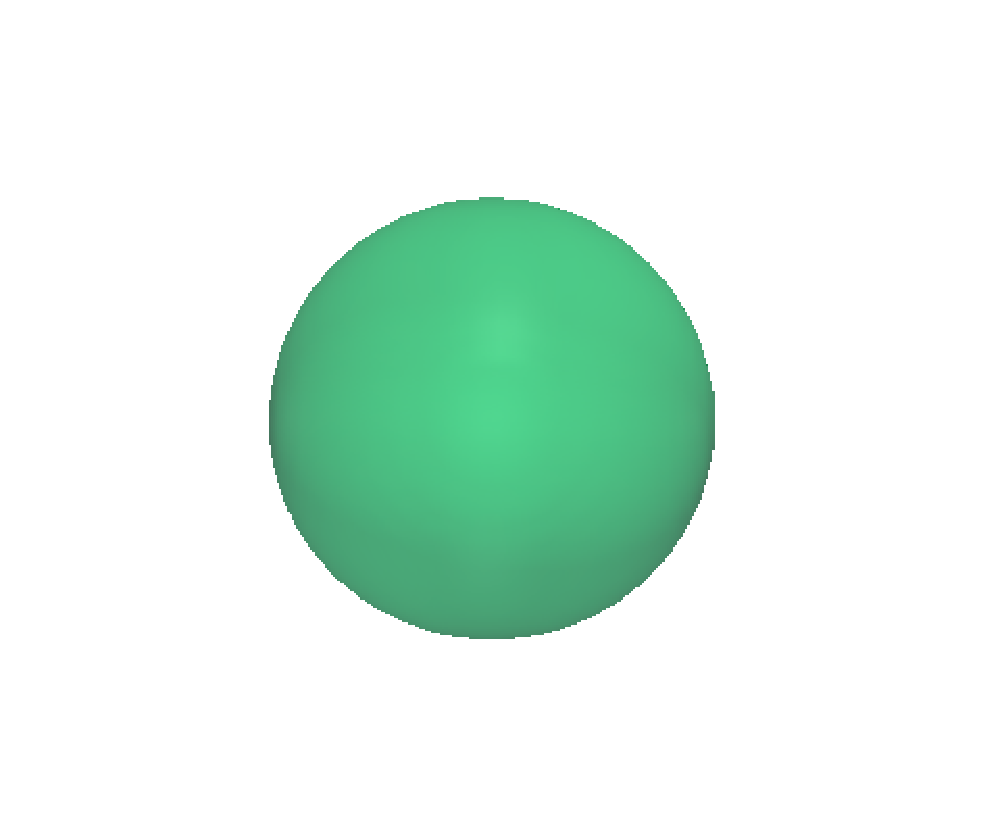
\includegraphics[width=.24\columnwidth]{Figures/Grace_sphr.pdf}}
    \subfigure[Ellipsoidal]{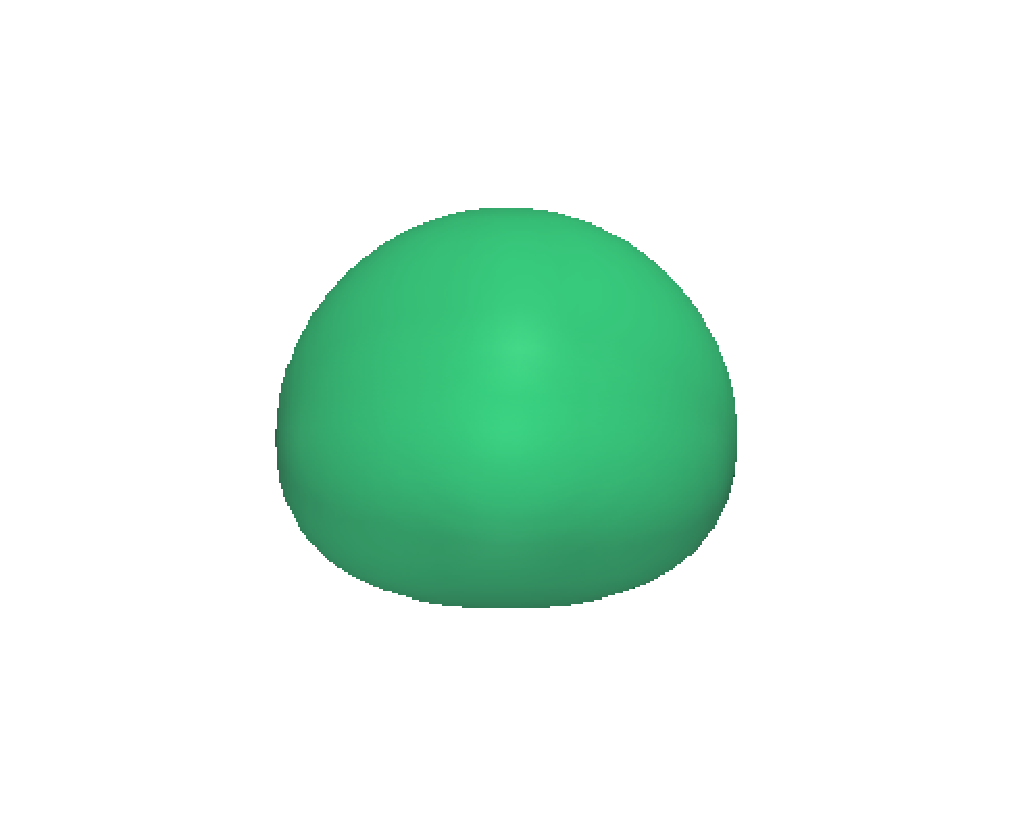
\includegraphics[width=.24\columnwidth]{Figures/Grace_ellip.pdf}}
    \subfigure[Skirted]{\includegraphics[width=.24\columnwidth]{Figures/Grace_skirt_t=10.png}}
    \subfigure[Dimpled]{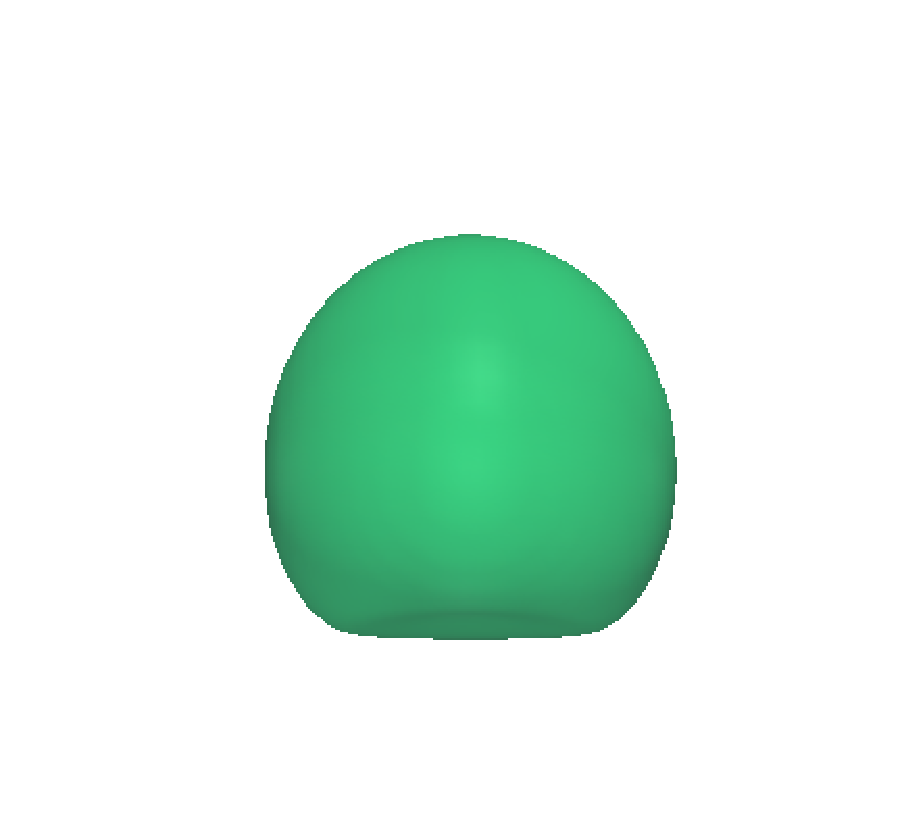
\includegraphics[width=.24\columnwidth]{Figures/Grace_dimp.pdf}}
    \caption{Bubble shapes resulting from different Morton (M) and Eotvos (Eo) numbers, as indicated in Table \ref{tab: bubble}.}
    \label{fig: bubble shape}
\end{figure}


%~~~~~~~~~~~~~~~~~~~~~~~%
%~~~~~~~~~~~~~~~~~~~~~~~%


\section{Droplet interactions}
\label{sec: idrop}

\Ge{A unique feature of colloidal suspensions is the interaction between neighboring droplets, displaying fascinating behaviors such as self-assembly, self-replication, \etc. The reason for such interactions is rather complex; it often arises from a combination of fluid mechanical effects and physicochemical properties of the substance. To study the droplet interactions in the present ICLS/NS framework, we provide in this section a hydrodynamic model for the depletion forces. The method is a natural extension of the LS and GFM, and we demonstrate the clustering of droplets in various structures from a dumbbell to a face-centered cubic crystal.}

\subsection{Extension to multiple level set}
\label{subsec: mls}

\Ge{The level set method discussed so far involves one marker function; we call it single level set (SLS) method. Thanks to its Eulerian nature, SLS can describe many droplets at the same time, provided that they do not need to be distinguished from each other. On the other hand,} 
%The present level set approach can be readily applied to the modeling of a single droplet or a number of droplets, thanks to its Eulerian nature. Since a single marker function is used, we call it single level set (SLS) method. 
SLS can also be extended to multiple level set (MLS), so that each droplet has its own color function. This has several benefits including distinction and tracking of each droplet, independent curvature computation, and ability to prevent numerical coalescence, \etc. Furthermore, with the narrow band approach \citep{Adalsteinsson_JCP_1995,Peng_JCP_1999} \Ge{and the various other techniques introduced in Sec.\ \ref{intro} \citep{Nielsen_JSC_2006,Brun_JCP_2012}}, the additional computational \Ge{and memory} cost as the number of the level set functions increases is limited.

%\begin{figure}[ht]
% \begin{center}
% \includegraphics[width=6cm]{Figures/mls.pdf}
% \end{center}
% \caption{MLS for different fluid phases. Colors indicate different material properties.}
% \label{fig: mls}
%\end{figure}

\begin{figure}[t]
 \begin{center}
 \includegraphics[width=5cm]{Figures/grid_mls.pdf}
 \end{center}
 \caption{Pressure jump in the presence of multiple interfaces within two grid cells. Red and blue circles indicate nodal pressure in droplet 1 and 2, respectively. (For interpretation of the references to color in this figure legend, the reader is referred to the web version of this article.)}
 \label{fig: GFM close}
\end{figure}

The extension from SLS to MLS is straightforward. Assuming no droplets will overlap, each level set function is simply advected successively. When two droplets get close (typically within two grid cells, see Fig.\ \ref{fig: GFM close}), the pressure jump across each interface needs to be considered and superimposed. That is, Eq.\ \eqref{laplace gfm} (corresponding to Fig.\ \ref{fig: GFM}) should be modified as
\begin{equation}
  \begin{aligned}
    (\nabla^2 p)_{i,j} & =\frac{p_{i-1,j} -2p_{i,j} +p_{i+1,j}}{\Delta x^2} 
                         -2\frac{[p]_{i,j}}{\Delta x^2} 
                         -\frac{1}{\Delta x} \bigg[\frac{\partial p}{\partial x} \bigg]_{i+1/2,j}
                         +\frac{1}{\Delta x} \bigg[\frac{\partial p}{\partial x} \bigg]_{i-1/2,j} \\
                       & +\frac{p_{i,j-1} -2p_{i,j} +p_{i,j+1}}{\Delta y^2}
                         -\frac{[p]_{i,j-1}}{\Delta y^2},
  \end{aligned}
  \label{laplace gfm mls}
\end{equation}
Similarly, all the jumps should be removed consistently when computing the pressure gradient in the subsequent step. \Ge{The above modification applies to both SLS and MLS, as the compact formulas (Eqs.\ \eqref{gfm+split projection} and \eqref{gfm+split correction}) remain the same; although MLS is clearly more accurate in resolving the near field structure.}

%~~~~~~~~~~~~~~~~~~~~~~~%

\subsection{Near-field interactions}
\label{subsec: pot}


\Ge{As introduced earlier, colloidal droplets transported in microfluidic devices are subject to various forces, a typical of which is the depletion force. The depletion force arises from the exclusion of the surfactant micelles in the colloidal suspension. It is often characterized as a near-field attracting potential \citep{Asakura_1958, Mewis_colloidal}, and plays a key role in the droplet dynamics \citep{Shen_AS_2016, Shen_thesis}.}
 Below, we first provide a brief background on the colloidal theory of the depletion potential, then present a numerical model to enforce the depletion force using MLS and GFM.

%~~~~~~~~~~~~~~~~~~~~~~~%

\subsubsection{The colloidal theory of the depletion potential}
\label{depletion theory}

\begin{figure}[t]

 \centering
 %\subfigure[]{\includegraphics[width=.5\columnwidth]{Figures/depletion2.pdf}}
 %\subfigure[]{\includegraphics[width=.3\columnwidth]{Figures/depl_model_zoom2.pdf}}
 \includegraphics[width=.75\columnwidth]{Figures/depletion3.pdf}
 %\includegraphics[width=8cm]{Figures/depletion.pdf}
 \caption{Depletion of surfactant micelles of radius $r_s$ between larger colloidal droplets of radius $R$, separated by distance $r$. The \Ge{dashed lines} around larger spheres represent the region from which the centers of small spheres are excluded. \Ge{They overlap when $r \leqslant 2R+2r_s$.} \Ge{Inset: a zoom-in sketch of two droplets near contact.}}
 \label{fig: overlap}
\end{figure}

The original depletion potential model proposed by \cite{Asakura_1958} assumes the surfactant micelles as non-interacting hard-spheres. As sketched in Fig.\ \ref{fig: overlap}, a suspension of such small spheres around the large colloidal droplets creates an osmotic pressure on the droplet surface. When the distance between two droplets is less than the diameter of the surfactant micelles, there will be a pressure defect due to the exclusion of the micelles, thus creating an attracting force. Integrating this force with respect to the inter-droplet distance $r$ leads to a potential energy
\begin{equation}
    U(r)=
    \begin{cases}
        \infty & \textrm{if} \quad r \leqslant 2R \\
        - p_{os}V_{ex} & \textrm{if} \quad 2R < r \leqslant 2R+2r_s  \\
        0 \quad & \textrm{otherwise}, \\
    \end{cases}
    \label{pot}
\end{equation}
where $V_{ex}$ is the excluded volume and $p_{os}$ is the osmotic pressure. 
\Ge{For spherical droplets, $V_{ex}$ can be calculated analytically}
\begin{equation}
    V_{ex}(r) = \frac{4\pi (R+r_s)^3}{3}\bigg[ 1- \frac{3r}{4(R+r_s)}+\frac{r^3}{16(R+r_s)^3} \bigg],
    \label{pot V}
\end{equation}
\Ge{where $R$ and $r_s$ are, respectively, the radii of the big and small spheres. The osmotic pressure is given as
\begin{equation}
    p_{os} = nkT,
    \label{pot P}
\end{equation}
where $n$ is the number density of the small spheres, $k$ is the Boltzmann constant, and $T$ is the temperature. The negative sign in Eq.\ \eqref{pot} corresponds to the tendency of the system to reduce its potential energy as the overlap increases. This is equivalent to increasing the total entropy of the small spheres \citep{Melby_PRL_2007}, and it provides a physical description of the depletion force even when the droplets are deformable, or when $p_{os}$ cannot be expressed by the van't Hoff's formula (Eq.\ \eqref{pot P}) \citep{Asakura_1958}.}


%~~~~~~~~~~~~~~~~~~~~~~~%

\subsubsection{A hydrodynamic model for the depletion force}

\Ge{Based on the above theory, the depletion force acting on a droplet is simply the derivative of the depletion potential, \ie $F(r)=dU/dr=-p_{os}dV_{ex}/dr$. However, $dV_{ex}/dr$ is not always straightforward to evaluate for non-spherical droplets; and unlike rigid-body dynamics, $F(r)$ cannot be applied directly to the motion of a liquid drop.
%Additionally, the rate of the variation of $V_{ex}(r)$ is not straightforward to evaluate if the droplets are deformed, as it is sometimes observed experimentally \citep{Shen_thesis}. 
In order to induce locally an aggregation, we take a closer look at the overlap region. As illustrated in Fig.\ \ref{fig: overlap}, when the surface distance between two colloidal droplets is less than $2r_s$, there is a small area in which the osmotic pressure is subject to a jump. Assuming the concentration of the surfactant micelles changes abruptly, it resembles the jump of the Laplace pressure; however, it will not generate any flow if the pressure is uniform in the depleted region. On the contrary, if the osmotic pressure varies continuously within the overlap, \ie $p'=p'(r')$, then we can write it as a Taylor-series expansion from $r'=r_s$
\begin{equation}
    p'(r'/r_s) = p'(1) + \bigg(\frac{r'}{r_s}-1 \bigg) \frac{\partial{p'}}{\partial{r'/r_s}},
    \label{pot P linear}
\end{equation}
where the distance to the droplet surface $r'$ is normalized by the surfactant micelle radius. An expansion of the osmotic pressure with the distance corresponds to a gradient of the micelle concentration near the gap. And if the micelle is much smaller than the droplet, as it is in many microfluidic devices \citep{Shen_AS_2016}, the gradient will be very sharp. Conversely, when the distance to the surface varies slowly, such as in the gap of a droplet and a flat wall, a uniform pressure will be recovered. Furthermore, a favorable pressure gradient from the overlap center will generate an outflow, pulling the droplets towards each other. Hence, Eq.\ \eqref{pot P linear} provides a hydrodynamic model for the depletion force.}

\Ge{In Eq.\ \eqref{pot P linear}, the gradient of the osmotic pressure $\partial{p'}/\partial{(r'/r_s)}$ is not known \textit{a priori}. It can be obtained by equating the depletion force acting on one droplet, \ie
\begin{equation}
    -p_{os}A_{ex} = \int_\Omega \big(p'(1) - p'(r'/r_s)\big)dS,
    \label{pot P balance}
\end{equation}
where $A_{ex}$ is the effective area of the overlap $\Omega$. Assuming a constant $\partial{p'}/\partial{(r'/r_s)}$, the above yields a linear dependence of the osmotic pressure on $r'$. Note that this is not the same as $p'$ varying linearly with the distance to the overlap center (see Fig.\ \ref{fig: overlap}). A description of the implementation and verification will be shown in the next section.}

\subsubsection{A MLS/GFM-based method for computing the depletion force}

\Ge{%The preceding model for the depletion force is written in 1D because of symmetry. In practice, droplets may deform due to other external forces and it is not always possible to define a symmetry axis. 
Provided a hydrodynamic model for the depletion force between two droplets, we can easily generalize it to multiple droplets using the MLS.
Thanks to the distance information embedded in the level set functions, it is straightforward to identify the overlap region of arbitrary geometries. Furthermore, as the jump of the osmotic pressure occurs only across the overlap shell, we can define
\begin{equation}
    [p']_\Omega = p'(r'/r_s) - p'(1),
    \label{pot P jump}
\end{equation}
similar to the Laplace pressure jump $[p]_\Gamma$ implemented by the GFM. Based on these observations, we propose a numerical method to compute the depletion force as laid out in Algorithm \ref{al: depletion}.}

\begin{algorithm}[t]
 Enter the pressure solver. Compute the right-hand side of Eq.\ \eqref{gfm+split projection}.\\ 
 \For{$m=1:(N-1)$}{
  Get the level set for droplet m, $\phi_m$.\\  
  \For{$n=(m+1):N$}{
   Get the level set for droplet n, $\phi_n$.\\   
    \textbf{where} $\phi_m<r_{s}$ and $\phi_n<r_{s}$ \textbf{do} $r'=(\phi_m+\phi_n)/2$, tag as \textit{overlap}.\\
    Compute $[p']_\Omega$ from Eqs.\ \eqref{pot P balance} and \eqref{pot P jump} within \textit{overlap}.\\
    \ForAll{$i,j,k$}{
     \eIf{entering overlap}{
     Add the osmotic pressure jump $[p']_{i,j,k}$.\\
     }{
     Remove the osmotic pressure jump $[p']_{i,j,k}$.\\
     }
    }
  }
 }
 Solve for $p^{n+1}$ regularly using the FastP* and GFM. Exit the pressure solver.\\
 \caption{A pseudo code for computing the depletion force.}
 \label{al: depletion}
\end{algorithm}

The overall idea of Algorithm \ref{al: depletion} is to enforce the depletion attraction in the projection step through the use of MLS and GFM. \Ge{Specifically, we first locate the overlap region of a pair of droplets with its own level set function, and define $r'$ as the average of the two distances. Then, Eq.\ \eqref{pot P balance} can be integrated numerically to obtain $\partial{p'}/\partial{(r'/r_s)}$, which together with Eqs.\ \eqref{pot P linear} and \eqref{pot P jump} gives $[p']_\Omega$. This variable pressure jump manifests itself as a modification term on the right-hand side of Eq.\ \eqref{gfm+split projection}, allowing us to use GFM to impose it across a sharp overlap shell. The resulting flow is divergence-free provided that all the jump terms are removed consistently in the correction step. Therefore, Eqs.\ \eqref{gfm+split projection} and \eqref{gfm+split correction} are re-formulated as 
\footnote[1]{\Ge{Eqs.\ \eqref{gfm+split correction} and \eqref{complete correction} are identical in form; however, $[p']_\Omega$ has to be removed when evaluating $\nabla_g p^{n+1}$ and $\nabla_g \hat{p}$ in Eq.\ \eqref{complete correction}, as it is done in Eq.\ \eqref{gfm grad}}}
\begin{equation}
    \nabla ^2 p^{n+1} = \nabla_g^2 ([p]_\Gamma+[p']_\Omega) 
    + \nabla \cdot \bigg[ \big(1-\frac{\rho_0}{\rho^{n+1}}) \nabla_g \hat{p} \bigg] + \frac{\rho_0}{\Delta t} \nabla \cdot {\bm u}^*,
  \label{complete projection}
\end{equation}}
and 
\begin{equation}
    {\bm u}^{n+1} = {\bm u}^* -\Delta t \bigg[\frac{1}{\rho_0} \nabla_g p^{n+1} + \big(\frac{1}{\rho^{n+1}} - \frac{1}{\rho_0}\big)\nabla_g \hat{p} \bigg].
  \label{complete correction}
\end{equation}


\noindent
\textbf{Approaching drops. } 
\Ge{We verify the depletion force model and its numerical implementation by simulating 2 to 14 approaching droplets in a quiescent fluid environment. Specifically, we set the droplet radius $R=0.5$, the computational domain $3\times3\times3$, and the resolution $\Delta x=1/32$. The radius of the surfactant micelle is set to be $r_s=1/16$, corresponding to $2\Delta x$. The viscosity and density ratios of the droplet to the ambient fluid are both 1. The non-dimensional parameters are %chosen as $Re=10$, $We=0.05$, 
$La=2000$
and $Fr=\infty$, leading to a reference Laplace pressure jump $p_\sigma=80$ and neglected gravity. The uniform osmotic pressure is either $10$ or $40$.}

\begin{figure}[t]
 \begin{center}
 %\includegraphics[width=\columnwidth]{Figures/min_dist.pdf}
  \includegraphics[width=\columnwidth]{Figures/min_dist2.pdf}

  \begin{picture}(0,0)
   \put(-70,60){\includegraphics[height=2cm]{Figures/2dp.png}}
   \put(100,60){\includegraphics[height=2cm]{Figures/3dp.png}}
  \end{picture}

 \end{center}
 \caption{Minimal distance between the droplet surfaces as function of time in the presence of depletion forces proportional to $p_{os}=10$ (solid line) and $p_{os}=40$ (dashed line). Simulation of (a) two droplets and (b) three droplets suspended in an initially quiescent fluid. Due to symmetry, only the minimal distance is plotted.}
 \label{fig: dep demo}
\end{figure}

\Ge{The temporal evolutions of the minimal surface distances in the case of two and three droplets are shown in Fig.\ \ref{fig: dep demo}. Here, time is scaled by a factor $T_\pi=(r_s/R)(p_\sigma/p_{os})$. The droplets, originally separated by a distance of $r_s$, get closer to the limit of the grid spacing at $t \approx T_\pi$. For the present study, we let the droplets aggregate without applying any repulsion models, except that the magnitude of the osmotic pressure is reduced when $d_{min}/r_s<0.1$. The smooth approaching in all cases and the collapse of the distance curve clearly evidence an attracting depletion force. To assess the robustness of the method, we further tested clustering of droplets into shapes from a 2D diamond to a face-centered cubic (FCC) composed of 14 drops, illustrated here in Fig.\ \ref{fig: clusters}. FCC represents the unit structure of one of the most compact sphere packings. Therefore, we can conclude that the hydrodynamic model implemented by the MLS/GFM-based method is accurate and robust in computing the depletion forces.}

\begin{figure}[t]
\centering
  \subfigure[Diamond]{\includegraphics[width=.2\columnwidth]{Figures/diamond.png}}
  \subfigure[Tetrahedron]{\includegraphics[width=.2\columnwidth]{Figures/tetrahedron.png}}
  \subfigure[Quintuplet]{\includegraphics[width=.2\columnwidth]{Figures/5-poly.png}}
  \subfigure[FCC]{\includegraphics[width=.2\columnwidth]{Figures/14-crystal.png}}
  \caption{\Ge{Examples of droplet clusters of different structures.}}
  \label{fig: clusters}
\end{figure}


%~~~~~~~~~~~~~~~~~~~~~~~%
%~~~~~~~~~~~~~~~~~~~~~~~%


\section{Conclusion}
\label{sec: conclusion}


A numerical method mainly intended for the hydrodynamic simulations of colloidal droplets in microfluidic devices has been developed and validated. The code is based on \Ge{an efficient and sharp} solver of the incompressible, two-fluid Navier-Stokes equations, and uses a mass-conserving level set method to capture the fluid interface. This combination provides a general framework for any multiphase flow problems (see \eg our recent study on jet instabilities \citep{Loiseau_PRF_2016}), and allows us to develop specific methods for the simulations of droplets in saturated surfactant suspensions with depletion forces as in the recent experiment in \cite{Shen_AS_2016}. Particularly, we have developed or extended four numerical techniques to improve the general accuracy:

\begin{enumerate}

    \item A mass-conserving, interface-correction level set method (ICLS) is proposed. As a standalone level set module, it is efficient, accurate, guarantees global mass conservation, and is simple to implement. It also enables corrections that can depend on the local curvature or any other parameter of interest. 
        
    \item A \Ge{geometric} estimation of the interface curvature based on nodal curvatures is introduced. As an important ingredient both for the mass correction (ICLS) and the surface tension computation, we show that the calculation converges in second-order both in 2D and 3D, and can lead to machine-zero spurious currents for a stationary 2D droplet.
    
    \item The ghost fluid method (GFM) for the computation of surface tension is combined with the FastP* method \citep{Dodd_JCP_2014}. This enables the use of \Ge{FFT-based solvers for a direct pressure solve}, and can accurately account for surface tension at large density ratios.
    
    \item A ghost fluid/multiple level set (GFM/MLS-based) method is also proposed to compute the \Ge{interaction force} caused by depletion potentials between multiple droplets or between droplets and a nearby wall. The approach can possibly be extended to account for surfactant diffusion at the interface and in the liquid.

\end{enumerate}

The last technique applies specifically to the simulation of colloidal droplets in microfluidic devices. This will enable us to further explore the effects of the near-field interactions as those observed experimentally in  \cite{Shen_AS_2016}, and potentially improve the design of microfluidic devices.
In addition, the combination of the GFM for sharp interfaces and the FastP* method \citep{{Dodd_JCP_2014}} can be exploited for the simulations of droplet in turbulent flows as in \cite{Dodd_JFM_2016}, adding an accurate representation of evaporation thanks to the ICLS approach proposed here.

%~~~~~~~~~~~~~~~~~~~~~~~%
%~~~~~~~~~~~~~~~~~~~~~~~%


\section*{Acknowledgments}

The work is supported by the Microflusa project. This effort receives funding from the European Union Horizon 2020 research and innovation programme under Grant Agreement No.\ 664823. O.T. acknowledges support from Swedish Research Council (VR) through the Grant Nr.\ 2013-5789. L.B. and J.-C.L. also acknowledge financial support by the European Research Council grant, no.\ ERC-2013-CoG-616186, TRITOS. The computer time was provided by SNIC (Swedish National Infrastructure for Computing).
Last but not least, Z.G. thanks Mehdi Niazi, Michael Dodd, Walter Fornari, Dr.\ Olivier Desjardins, Dr.\ S\'{e}bastien Tanguy, Dr.\ Marcus Herrmann, and Dr.\ David Salac for interesting and helpful discussions. 





%% --------------------------------------------------------------------------- %%

%% The Appendices part is started with the command \appendix;
%% appendix sections are then done as normal sections
\appendix

\section{\Ge{Discretization error of $\int_\Gamma {\bm n}\cdot{\bm u}_c d\Gamma$}}
\label{appendix-dis_err}
\Ge{
Similar to \cite{Engquist_JCP_2005}, we define the discretization error
\begin{equation}
    E= \bigg| \bigg( \prod_{k=1}^{d} \Delta x_{k} \bigg) \sum_{j \in Z^d} \hat{\delta}_\epsilon (\Gamma,g,{\bm x}_j)
    -\int_\Gamma {\bm n}\cdot{\bm u}_c d\Gamma \bigg|,
  \label{app-def}
\end{equation}
where $\hat{\delta}_\epsilon$ is a Dirac delta function of variable strength $g$ supported on the surface $\Gamma$, and ${\bm x} \in \mathbb{R}^d$. Following the derivations in Sec.\ \ref{subsec: ICLS}, the extension of $g$ to $\mathbb{R}^d$ is provided by Eq.\ \eqref{correction vel sol}, allowing one to write
\begin{equation}
    E= \bigg|\bigg( \prod_{k=1}^{d} \Delta x_{k} \bigg) 
    \sum_{j \in Z^d} \frac{\delta V}{\delta t} \frac{f_s \delta_\epsilon(\phi({\bm x}_j))|\nabla \phi({\bm x}_j)|}{A_f} 
    -\int_\Gamma {\bm n}\cdot{\bm u}_c d\Gamma \bigg|.
  \label{app-step1}
\end{equation}
Here, $\delta_\epsilon(\phi)$ is a one dimensional regularized delta function depending on the level set $\phi$, and the expression is simplified noting that $\bm{n} \cdot \nabla{\phi} = |\nabla \phi|$ (it does not have to be a distance function). By definition, $A_f=\int_\Gamma f_s \delta_\epsilon (\phi) |\nabla \phi| \,d\Gamma$, discretely reducing Eq.\ \eqref{app-step1} to
\begin{equation}
    E= \bigg| \frac{\delta V}{\delta t}
    -\int_\Gamma {\bm n}\cdot{\bm u}_c d\Gamma \bigg|.
  \label{app-step2}
\end{equation}
Comparing with Eq.\ \eqref{vol change}, it is obvious that $E=0$. That is, the discretization error of $\int_\Gamma {\bm n}\cdot{\bm u}_c d\Gamma$ used in the mass correction is identically zero, independent of the choice of the regularized delta function.
}


%--%%% --------------------------------------------------------------------------- %%
%--%
%--%%% References
%--%%%
%--%%% Following citation commands can be used in the body text:
%--%%% Usage of \cite is as follows:
%--%%%   \cite{key}         ==>>  [#]
%--%%%   \cite[chap. 2]{key} ==>> [#, chap. 2]
%--%%%
%--%
%--%%% References with bibTeX database:
%--%
%--%%\bibliographystyle{plain}
%--%\bibliographystyle{elsarticle-num}
%--%
%--%% \bibliographystyle{elsarticle-harv}
%--%% \bibliographystyle{elsarticle-num-names}
%--%% \bibliographystyle{model1a-num-names}
%--%% \bibliographystyle{model1b-num-names}
%--%% \bibliographystyle{model1c-num-names}
%--%% \bibliographystyle{model1-num-names}
%--%% \bibliographystyle{model2-names}
%--%% \bibliographystyle{model3a-num-names}
%--%% \bibliographystyle{model3-num-names}
%--%% \bibliographystyle{model4-names}
%--%% \bibliographystyle{model5-names}
%--%% \bibliographystyle{model6-num-names}
%--%
%--%\bibliography{1}
%--%
%--%
%--%\end{document}
%--%
%--%%%
%--%%% End of file `elsarticle-template-num.tex'.



%------------------------------------------------------------------------------
% Bibliography
%------------------------------------------------------------------------------
%
%\clearpage
\bibliographystyle{jfm}
\bibliography{thesis}
%
\IfFileExists{paper1/paper.bbl}{%------------------------------------------------------------------------------
% Define title, author(s), affiliation and publishing status
%
\papertitle[ICLS/GFM for droplet suspensions under depletion forces] % Short title used in headlines (optional)
{%
  An efficient mass-preserving interface-correction level set/ghost fluid method
  for droplet suspensions under depletion forces% THE COMMENT SYMBOL AT THE END OF THIS LINE IS NEEDED
}%
%
\papertoctitle{An efficient mass-preserving interface-correction level set/ghost fluid method
  for droplet suspensions under depletion forces} % Title for toc
%
\paperauthor[Ge, Loiseau, Tammisola, Brandt] % Short authors used in headlines and List Of Papers
{%
  Zhouyang Ge, Jean-Christophe Loiseau, Outi Tammisola, Luca Brandt%
}%
%
\listpaperauthor{Z. Ge, J-Ch. Loiseau, O. Tammisola, L. Brandt}% (optional) Short authors used in List Of Papers
%
\paperaffiliation
{%
  Linn\'e FLOW Centre and SeRC, KTH Mechanics, S-100 44 Stockholm, Sweden%
}%
%
\paperjournal[J. Comput. Phys.] % Short publish info used in List Of Papers
{%
	Journal of Computational Physics%
}%
%
\papervolume{353}%
%
\papernumber{}%
%
\paperpages{435--459}%
%
\paperyear{2018}%
%
\papersummary%
{% Insert summary of the paper here (used in introduction)
In this first work, we develop and implement an interface-correction level set/ghost fluid method (\texttt{ICLS/GFM})
for high-fidelity simulations of liquid droplets in an immiscible carrier fluid.
The main novelty is a global mass correction scheme that is conceptually simple,
relatively straightforward to program,
and efficient since the scheme does not need to be excuted at every time step.
The method works best for well-resolved droplets as validated in the paper;
however, extra care must be taken when applying it otherwise.
In the same paper, we also formulate a hydrodynamic model for surfactant-induced depletion forces between neighbouring drops,
removing the need to simulate suspending surfactants,
hence further improving the computational efficiency.
The overall methodology can be readily used to study droplet interactions in liquid flows,
and may be extended to simulate multiphase flows in porous media in general.
}%
%
\graphicspath{{paper1/}}%
%
%
%===============================================================================
%                            BEGIN PAPER
%===============================================================================
%
\begin{paper}

\makepapertitle

%------------------------------------------------------------------------------
% Abstract
%------------------------------------------------------------------------------
%
\begin{paperabstract}
Aiming for the simulation of colloidal droplets in microfluidic devices, we present here a numerical method for two-fluid systems subject to surface tension and depletion forces among the suspended droplets. The algorithm is based on an efficient solver for the incompressible two-phase Navier-Stokes equations, and uses a mass-conserving level set method to capture the fluid interface. 
The four novel ingredients proposed here are, firstly, an interface-correction level set (ICLS) method; % that efficiently preserves mass. 
global mass conservation is achieved by performing an additional advection near the interface, with a correction velocity obtained by locally solving an algebraic equation, which is easy to implement in both 2D and 3D. 
Secondly, we report a second-order accurate geometric estimation of the curvature at the interface and, 
thirdly, the combination of the ghost fluid method with the fast pressure-correction approach enabling an accurate and fast computation even for large density contrasts. 
Finally, we derive %sharp formulation for the pressure difference 
a hydrodynamic model for the interaction forces
induced by depletion of surfactant micelles and combine it with a multiple level set approach to study short-range interactions among droplets in the presence of attracting forces.
        \keywords{Multiphase flow, Level set method, Ghost fluid method, Droplet, Depletion force}
\end{paperabstract}


%------------------------------------------------------------------------------
% Article
%------------------------------------------------------------------------------
%
%--%%%
%--%%% Copyright 2007, 2008, 2009 Elsevier Ltd
%--%%%
%--%%% This file is part of the 'Elsarticle Bundle'.
%--%%% ---------------------------------------------
%--%%%
%--%%% It may be distributed under the conditions of the LaTeX Project Public
%--%%% License, either version 1.2 of this license or (at your option) any
%--%%% later version.  The latest version of this license is in
%--%%%    http://www.latex-project.org/lppl.txt
%--%%% and version 1.2 or later is part of all distributions of LaTeX
%--%%% version 1999/12/01 or later.
%--%%%
%--%%% The list of all files belonging to the 'Elsarticle Bundle' is
%--%%% given in the file `manifest.txt'.
%--%%%
%--%
%--%%% Template article for Elsevier's document class `elsarticle'
%--%%% with numbered style bibliographic references
%--%%% SP 2008/03/01
%--%%%
%--%%%
%--%%%
%--%%% $Id: elsarticle-template-num.tex 4 2009-10-24 08:22:58Z rishi $
%--%%%
%--%%%
%--%\documentclass[preprint,12pt,3p]{elsarticle}
%--%
%--%%% My packages
%--%
%--%\usepackage{fullpage}
%--%\usepackage{graphicx}
%--%\usepackage{subfigure}
%--%\usepackage{amsfonts}
%--%\usepackage{amsgen}
%--%\usepackage{amsbsy}
%--%\usepackage{amsmath}
%--%\usepackage{amssymb}
%--%\usepackage{mathrsfs}
%--%\usepackage{mathtools}
%--%\usepackage{bm}
%--%\usepackage{epstopdf}
%--%\usepackage{caption}
%--%\usepackage{tabularx}
%--%\usepackage{tabu}
%--%\usepackage{xcolor}
%--%\usepackage{nicefrac}
%--%\usepackage{enumitem}
%--%\usepackage[ruled]{algorithm2e}
%--%%\usepackage[colorlinks=false]{hyperref} % link eq./fig./tab.
%--%\usepackage{url}
%--%
%--%\newcommand{\lb}[1]{\textcolor{red}{#1}}
%--%\newcommand{\Ge}[1]{\textcolor{black}{#1}}
%--%
%--%\newcommand\etal{\textit{et al }}
%--%\newcommand\ie{\textit{i.e. }}
%--%\newcommand\viz{\textit{viz. }}
%--%\newcommand\eg{\textit{e.g. }}
%--%\newcommand{\e}[1]{\ensuremath{\times 10^{#1}}}
%--%\newcommand\etc{\textit{etc}}
%--%\DeclarePairedDelimiter\abs{\lvert}{\rvert}
%--%
%--%\bibliographystyle{unsrt}  % references listed in order of appearance
%--%
%--%%% End my packages
%--%
%--%
%--%%% Use the option review to obtain double line spacing
%--%%% \documentclass[preprint,review,12pt]{elsarticle}
%--%
%--%%% Use the options 1p,twocolumn; 3p; 3p,twocolumn; 5p; or 5p,twocolumn
%--%%% for a journal layout:
%--%%% \documentclass[final,1p,times]{elsarticle}
%--%%% \documentclass[final,1p,times,twocolumn]{elsarticle}
%--%%% \documentclass[final,3p,times]{elsarticle}
%--%%% \documentclass[final,3p,times,twocolumn]{elsarticle}
%--%%% \documentclass[final,5p,times]{elsarticle}
%--%%% \documentclass[final,5p,times,twocolumn]{elsarticle}
%--%
%--%%% if you use PostScript figures in your article
%--%%% use the graphics package for simple commands
%--%%% \usepackage{graphics}
%--%%% or use the graphicx package for more complicated commands
%--%%% \usepackage{graphicx}
%--%%% or use the epsfig package if you prefer to use the old commands
%--%%% \usepackage{epsfig}
%--%
%--%%% The amssymb package provides various useful mathematical symbols
%--%\usepackage{amssymb}
%--%%% The amsthm package provides extended theorem environments
%--%%% \usepackage{amsthm}
%--%
%--%%% The lineno packages adds line numbers. Start line numbering with
%--%%% \begin{linenumbers}, end it with \end{linenumbers}. Or switch it on
%--%%% for the whole article with \linenumbers after \end{frontmatter}.
%--%%% \usepackage{lineno}
%--%
%--%%% natbib.sty is loaded by default. However, natbib options can be
%--%%% provided with \biboptions{...} command. Following options are
%--%%% valid:
%--%
%--%%%   round  -  round parentheses are used (default)
%--%%%   square -  square brackets are used   [option]
%--%%%   curly  -  curly braces are used      {option}
%--%%%   angle  -  angle brackets are used    <option>
%--%%%   semicolon  -  multiple citations separated by semi-colon
%--%%%   colon  - same as semicolon, an earlier confusion
%--%%%   comma  -  separated by comma
%--%%%   numbers-  selects numerical citations
%--%%%   super  -  numerical citations as superscripts
%--%%%   sort   -  sorts multiple citations according to order in ref. list
%--%%%   sort&compress   -  like sort, but also compresses numerical citations
%--%%%   compress - compresses without sorting
%--%%%
%--%%% \biboptions{comma,round}
%--%
%--%% \biboptions{}
%--%
%--%
%--%\journal{Journal of Computational Physics}
%--%
%--%\begin{document}
%--%
%--%\begin{frontmatter}
%--%
%--%\title{An efficient mass-preserving interface-correction level set/ghost fluid method for droplet suspensions under depletion forces}   %\tnoteref{label0}}
%--%%\tnotetext[label0]{This is only an example}
%--%
%--%  %1
%--%  \author[]{Zhouyang Ge\corref{cor1}}
%--%  %\address[label1]{Linn\'e Flow Centre and SeRC (Swedish e-Science Research Centre), KTH Mechanics, \\ S-100 44 Stockholm, Sweden}
%--%  \cortext[cor1]{Corresponding author.}
%--%  %\fntext[label4]{Small city}
%--%  \ead{zhoge@mech.kth.se}
%--%  %\ead[URL]{https://sites.google.com/site/mlsgfm/}
%--%  
%--%  %2
%--%  \author[]{Jean-Christophe Loiseau\fnref{label2}}
%--%  \fntext[label2]{Present address: Laboratoire DynFluid, Arts et M\'etiers ParisTech, 151 boulevard de l'h\^opital, 75013 Paris, France}
%--%  \ead{jean-christophe.loiseau@ensam.eu}
%--%  
%--%  %3
%--%  \author[]{Outi Tammisola}
%--%  %\address[label3]{Faculty of Engineering, The University of Nottingham, NG72RD Nottingham, UK}
%--%  \ead{outi@mech.kth.se}
%--%  
%--%  %4
%--%  \author[]{Luca Brandt}
%--%  \ead{luca@mech.kth.se}
%--%
%--%  \address{Linn\'e Flow Centre and SeRC (Swedish e-Science Research Centre), KTH Mechanics, \\ S-100 44 Stockholm, Sweden}
%--%
%--%\sloppy
%--%\begin{abstract}
%--%Aiming for the simulation of colloidal droplets in microfluidic devices, we present here a numerical method for two-fluid systems subject to surface tension and depletion forces among the suspended droplets. The algorithm is based on \Ge{an efficient} solver for the incompressible two-phase Navier-Stokes equations, and uses a \Ge{mass-conserving} level set method to capture the fluid interface. 
%--%The four novel ingredients proposed here are, firstly, an interface-correction level set (ICLS) method; % that efficiently preserves mass. 
%--%global mass conservation is achieved by performing an additional advection near the interface, with a correction velocity obtained by locally solving an algebraic equation, which is easy to implement in both 2D and 3D. 
%--%Secondly, we report a second-order accurate \Ge{geometric} estimation of the curvature at the interface and, 
%--%thirdly, the combination of the ghost fluid method with the fast pressure-correction approach enabling an accurate and fast computation even for large density contrasts. 
%--%Finally, we derive %sharp formulation for the pressure difference 
%--%\Ge{a hydrodynamic model for the interaction forces}
%--%induced by depletion of surfactant micelles and combine it with a multiple level set approach to study short-range interactions among droplets in the presence of attracting forces.
%--%\end{abstract}
%--%
%--%\begin{keyword}
%--%%% keywords here, in the form: keyword \sep keyword
%--%Multiphase flow \sep Level set method \sep Ghost fluid method \sep Colloidal droplet
%--%%% MSC codes here, in the form: \MSC code \sep code
%--%%% or \MSC[2008] code \sep code (2000 is the default)
%--%\end{keyword}
%--%
%--%\end{frontmatter}
%--%
%--%%%
%--%%% Start line numbering here if you want
%--%%%
%--%% \linenumbers


%% --------------------------------------------------------------------------- %%

%% main text

\section{Introduction}
\label{intro}

In the field of colloidal science, much progress has been made on the synthesis of elementary building blocks \Ge{(Fig.\ \ref{fig:exp})} mimicking molecular structures to elaborate innovative materials, \eg materials with complete three dimensional band gaps \citep{Xia_etal_AM2000, Velev_etal_AM2009, Li_etal_AC2011, Sacanna_etal_COCIS2011}. The basic elements of such colloidal molecules are particles or droplets less than one millimeter in size, and their self-assembly relies on either lengthy brownian motion or careful microfludic designs, on top of typical colloidal interactions, \eg depletion attraction and electrostatic repulsion \citep{Mewis_colloidal, Yi_etal_CM2013, Shen_AS_2016}. Regardless of the approach, however, questions remain why the colloidal particles/droplets undergo certain path to organize themselves and how such process can be controlled and optimized. Since full data are not yet accurately accessible from experiments in such miniature systems, computer simulations will be useful to provide supplemental information.

\begin{figure}[t!]
\centering
  \includegraphics[width=.8\columnwidth]{Figures/experimental_clusters.pdf}
  \caption{\Ge{Self-assembled colloidal clusters. a) Electron micrograph of a suspension of triplet clusters. Scale bar, 30 $\mu$m. b-e) Close up of doublet, triplet, quadruplet, and quintuplet clusters. Scale bars, 10 $\mu$m. Further details are available in \cite{Shen_AS_2016}, photograph courtesy of Dr.\ Joshua Ricouvier.}}
  \label{fig:exp}
\end{figure}

Scaling down to microscale appears first to be a convenience for the numerical simulations of multicomponent and multiphase systems as the non-linear Navier-Stokes (NS) equations can be reduced to the linear Stokes equations. This allows the use of boundary integral methods (BIM) \citep{Pozrikidis}, \eg most recently the GGEM-based BIM \citep{Kumar_JCP_2012, Lailai_SM_2014} solving the Stokes equations in general geometries. However, it is also possible to use the conventional unsteady, fractional-step/projection-method NS solver at low Reynolds number, combined with an interface description method \citep{Worner_2012, Galusinski_JCP_2008}. The latter approach is more versatile, probably less difficult to implement, and enjoys a rich literature of standard numerical techniques. Here, in view of a rich range of possible applications and considering also the rapid development of inertial microfluidics (where inertial effects are used to better control the flow behavior) we take the approach of simulating the incompressible, two-fluid NS as outlined in \cite{Dodd_JCP_2014}. The splitting procedure proposed in \cite{Dodd_JCP_2014} enables the use of fast solvers for the pressure Poisson equation also for large density and viscosity contrasts. The remaining choice then is to be made among the available interface-description methods. 

Generally, there are two categories of methods to resolve an interface in a NS solver, \ie front-tracking methods and front-capturing methods. An example of the front-tracking method is the immersed boundary method (IBM) \Ge{\citep{Peskin,Uhlmann}. Using Lagrangian points in a moving frame, IBM can offer a high interface resolution without the need to deform the underlying mesh in the fixed frame. However, the coupling of the two meshes relies on a regularized delta function, which introduces certain degrees of smearing. Moreover, large interface deformation requires frequent mesh rearrangement; and topology changes may have to be handled manually. These constraints make IBM typically more expensive and less appealing for droplet simulations.}

Front-capturing methods, on the other hand, are Eulerian and handle topology changes automatically; they are therefore easier to parallelize to achieve higher efficiency. One of such methods is the volume-of-fluid (VOF) method \citep{Scardovelli_ARFM_1999}, which defines different fluids with a discontinuous color function. The main advantage of VOF is its intrinsic mass conservation. It suffers however from inaccurate computations of the interface properties, \eg normals and curvatures. This makes it less favorable for simulations of microfluidic systems where surface tension \Ge{is the dominant effect and requires accurate modelling.}

Another popular front-capturing method is the level set (LS) method \citep{Sethian_levelset, Sussman_JCP_1994}. Contrary to VOF, LS prescribes the interface through a \Ge{(Lipschitz-)continuous} function which usually takes the form of the signed distance to the interface. \Ge{Under this definition}, normals and curvatures of the interface can be readily and accurately computed. However, the problem when simulating incompressible flows is that mass loss/gain may occur and accumulate because the LS function embeds no volume information. \Ge{In addition, errors can also arise from solving the LS advection equation and/or the reinitialization equation,} a procedure commonly required to reshape the LS into a distance function. Therefore, additional measures have to be taken to ensure mass conservation.

Many different approaches have been proposed to make LS mass-conserving, which can be classified into the following \Ge{four} methodologies. The first approach is to improve the LS discretization and reinitialization so that numerical errors are reduced. In practice, one can increase the order of LS fluxes \citep{Nourgaliev_JCP_2007}, minimize the displacement of the zero LS during reinitialization \Ge{\citep{Russo_JCP_2000,Nourgaliev_JCP_2007}}, or employ local mesh refinement \Ge{\citep{Strain_JCP_1999b,Min_JCP_2007,Herrmann_JCP_2008}}. By doing so, mass loss can be greatly reduced, although the LS function is still inherently non-conservative. The second remedy couples the LS with \Ge{a conservative description (\eg VOF) or Lagrangian particles.} For example, \Ge{the hybrid particle level set method \citep{Enright_JCP_2002},} the coupled level set volume-of-fluid (CLSVOF) method \citep{Sussman_JCP_2000}, the mass-conserving level set (MCLS) method \citep{Pijl_CVS_2008}, or the recent curvature-based mass-redistribution method \citep{Luo_JCP_2015}. With varying level of coupling, \Ge{these methods can usually preserve mass really well; the drawback is that the complexity and some inaccuracy (due to interpolation, reconstruction, \etc) of the other method will be imported. The third approach improves mass conservation by adding a volume-constraint in the LS or NS formulation. Examples of this kind include the interface-preserving LS redistancing algorithm \citep{Sussman_JSC_1997} and the mass-preserving NS projection method \citep{Salac_CPC_2016}. Finally, one can also smartly modify the definition of the LS, such as the hyperbolic-tangent level set \citep{Olsson_JCP_2005}, to reduce the overall mass loss.}
%the extension-velocity level set \citep{Sabelnikov_JCP_2014}, 

With the physical application of colloidal droplets in mind, 
\Ge{and using ideas from some of the above-mentioned methods, we heuristically propose an interface-correction level set (ICLS) method.} The essential idea of ICLS is to construct a normal velocity supported on the droplet interface and use it in an additional LS advection to compensate for mass loss, in a way similar to inflating a balloon. Because no coupling with VOF \Ge{or Lagrangian particles} is required, the simplicity and high accuracy of the original LS method is preserved, yet the extra computational cost of this procedure is negligible.

%Based on the newly proposed ICLS method, we extend the single level set (SLS) to multiple level set (MLS) functions. MLS has the benefits that each droplet \Ge{within a colloidal cluster} can be treated individually, is allowed to interact with the other droplets, and is guarded from its own mass loss. MLS also prevents numerical coalescence of droplets when they get too close. \Ge{The computational complexity, proportional to the number of MLS functions ($l$) and the number of cells in each dimension ($N$), is higher than SLS. However, we note that many techinques exist to reduce the CPU cost and/or memory consumption if $lN^d$ ($d=$ 2 or 3) is large. For detailed implementations of such optimized algorithms we refer to \cite{Peng_JCP_1999,Nielsen_JSC_2006,Brun_JCP_2012}. In the present paper, we will demonstrate our method using one droplet per MLS function.}

\Ge{Provided a mass-preserving level set method, the coupled flow solver must also accurately compute the surface tension, a singular effect of the normal stress on the interface. This is particularly important for microfluidic systems; as surface tension scales linearly with the dimension, it decays slower than volumetric forces (\eg gravity) when the size of the system reduces.}
%One difficulty of the simulation of multiphase flow is the presence of surface tension, which manifests itself as a pressure jump across an infinitesimally thin interface. In microfluidic systems, particularly, surface tension becomes more prominent since it scales linearly with the dimension of the system (hence diminishes slower than volumetric forces such as gravity).  
To handle such discontinuities, one approach is the continuum surface force (CSF) \citep{Brackbill_JCP_1992}, \Ge{originally developed for the VOF method, later extended to the LS \citep{Sussman_JCP_1994}.} 
%which smears out the pressure difference and models the surface tension as a smoothed forcing term. 
\Ge{Although easy to implement}, CSF effectively introduces an artificial spreading of the interface \Ge{by regularizing the pressure difference}, and it can become erroneous when two interfaces are within its smoothing width.
%Another interesting technique, in the context of finite-difference discretizations of the NS equations, 
\Ge{A second, non-smearing approach is the ghost fluid method (GFM). Proposed initially for solving compressible Euler equations \citep{Fedkiw_JCP_1999}, GFM provides a finite-difference discretization of the gradient operator even if the stencil includes shocks. It has been proven to converge \citep{Liu_MC_2003} and was soon applied for treating the pressure jump in multiphase flows \citep{Kang_JSC_2000}. We note that although the GFM can be reformulated in a similar way to the CSF \citep{Lalanne_JCP_2015,Popinet_ARFM_2018}, its treatment for discontinuous quantities is sharp in the finite difference limit.} 

\Ge{Several implementation options of the GFM were suggested in \cite{Kang_JSC_2000,Lalanne_JCP_2015,Desjardins_JCP_2008}. Here, we follow the methodology of \cite{Desjardins_JCP_2008}, \ie using the GFM for the pressure jump due to surface tension while neglecting the viscous contribution. As will be discussed later, this choice is especially suitable for microfluidic applications where the capillary effect is strong.}
% result in a second-order accurate pressure field, while preserving the discontinuity for both pressure and density. Their original algorithm is framed for solving the pressure Poisson equation iteratively, \eg through a multi-grid solver. Here, we first propose a second-order accurate, grid-converging interface curvature estimation, and then adapt it to a fast pressure-correction method (FastP*) \cite{Dodd_JCP_2014} that benefits from an efficient, FFT-based, direct solver. The only additional requirement from \cite{Dodd_JCP_2014} is that the computational domain is periodic in at least two directions. 
\Ge{To efficiently solve for the pressure, we further combine the GFM with a fast pressure-correction method (FastP*) \citep{Dodd_JCP_2014}. Such a combination enables a direct solve of the pressure Poisson equation using the Gauss elimination in the Fourier space; it is the most efficient when the computational domain is periodic, but it also applies to a range of homogeneous Dirichlet/Neumann boundary conditions via fast sine/cosine transforms \citep{Schumann_JCP_1988}, see \eg a recent open-source distribution \citep{Pedro_CaNS}. Using a second-order accurate, grid-converging interface curvature estimation, we will show that the coupled ICLS/NS solver can handle large density/viscosity contrasts and converges between first and second order in both space and time.}

Finally, a unique challenge to the simulation of colloidal droplets is the modeling of near-field interactions. It is known that two or more colloids can interact via dispersion, surface, depletion, and hydrodynamic forces \citep{Mewis_colloidal}. Apart from the hydrodynamic forces which is determined directly from the NS, and the dispersion forces which arise from quantum mechanical effects, the depletion and surface forces must be modelled. These forces can be either attraction or repulsion and are typically calculated from the gradient of a potential.
\Ge{Based on colloidal theory, we propose a novel hydrodynamic model for the depletion force in the framework of the ICLS/NS solver. Our method relies on two extensions: \textit{i)} extending the single level set (SLS) function to multiple level set (MLS) functions; and \textit{ii)} extending the GFM for computation of the gradient of depletion potential. 
MLS has the benefits that each droplet within a colloidal cluster can be treated individually, is allowed to interact with the other droplets, and is guarded from its own mass loss. MLS also prevents numerical coalescence of droplets when they get too close. The computational complexity, proportional to the number of MLS functions ($l$) and the number of cells in each dimension ($N$), is higher than SLS. However, we note that many techniques exist to reduce the CPU cost and/or memory consumption if $lN^d$ ($d=$ 2 or 3) is large. For detailed implementations of such optimized algorithms we refer to \cite{Peng_JCP_1999,Nielsen_JSC_2006,Brun_JCP_2012}. In the present paper, we will demonstrate the self-assembly of colloidal droplets using one droplet per MLS function.}
%Hence, MLS is needed to determine the interaction forces. Combining with GFM, we propose a novel method to compute the near field interactions in our NS solver. The GFM makes the interaction force sharp and the MLS makes it possible for two droplets to be closer than one grid cell without automatic merging.

The paper is organized as follows. In Sec.\ \ref{subsec: gov eqns}, the governing equations for the incompressible, two-phase flow are briefly presented. In Sec.\ \ref{subsec: dls}, the classical signed-distance LS methodology \Ge{together with some commonly used numerical schemes is discussed.} \Ge{We then introduce the ICLS method in Sec.\ \ref{subsec: ICLS}, starting from the derivation ending with a demonstration. We further provide a geometric estimation of the interface curvature tailored to the GFM in Sec.\ \ref{subsec: curv}. The complete ICLS/NS solver is outlined in Sec.\ \ref{subsec: NS}, including a detailed description of the implementation and three examples of validation.} In Sec.\ \ref{sec: idrop}, we propose a MLS/GFM-based method for the modeling of near-field depletion potential. \Ge{Finally, we summarize the overall methodology in Sec.\ \ref{sec: conclusion}.}
%we derive an interface curvature estimation and demonstrate its second-order convergence. Our coupled flow solver is outlined in Sec.\ \ref{subsec: NS} along with three validation cases. Finally, we propose a MLS/GFM-based method for the modeling of near-field depletion potential in Sec.\ \ref{sec: idrop}.


%~~~~~~~~~~~~~~~~~~~~~~~%
%~~~~~~~~~~~~~~~~~~~~~~~%


\section{Governing equations for interfacial two-phase flow}
\label{subsec: gov eqns}

The dynamics of the incompressible flow of two immiscible fluids is governed by the Navier-Stokes equations, written in the non-dimensional form

\begin{subequations}
 \begin{equation}
   \nabla \cdot {\bm u} = 0,
  \label{div free}
 \end{equation}

 \begin{equation}
      \frac{\partial {\bm u}}{\partial t} + {\bm u} \cdot \nabla {\bm u} = \frac{1}{\rho_i} \bigg(-\nabla p + \frac{1}{Re} \nabla \cdot \big[ \mu_i ( \nabla {\bm u} + \nabla {\bm u}^T ) \big] \bigg) + \frac{1}{Fr}{\bm g},
  \label{NS}
 \end{equation}
\end{subequations}

\noindent where ${\bm u}={\bm u}({\bm x},t)$ is the velocity field, $p=p({\bm x},t)$ is the pressure field, and $\bm{g}$ is a unit vector aligned with gravity or buoyancy. $\rho_i$ and $\mu_i$ are the density and dynamic viscosity ratios of fluid $i$ ($i=1$ or $2$) and the reference fluid. These properties are \Ge{constant in each phase and} subject to a jump across the interface, which we denote as $[\rho]_\Gamma=\rho_2-\rho_1$ for density and $[\mu]_\Gamma=\mu_2-\mu_1$ for viscosity. For viscous flows, the velocity and its tangential derivatives are continuous on the interface \citep{Liu_JCP_1994}. However, the pressure is discontinuous due to the surface tension and the viscosity jump, \ie
\begin{equation}
    [p]_\Gamma = \frac{1}{We} \kappa + \frac{2}{Re}[\mu]_\Gamma {\bm n}^T \cdot \nabla {\bm u} \cdot {\bm n},
  \label{pressure jump}
\end{equation}
\noindent where $\kappa$ is the interface curvature, and ${\bm n}$ is the normal to the interface.  
If the surface tension coefficient, $\tilde{\sigma}$, varies on the interface the tangential stress is also discontinuous. In this paper, we assume constant and uniform $\tilde{\sigma}$. In Eqs.\ \eqref{NS} and \eqref{pressure jump}, Re, We, and Fr are, respectively, the Reynolds, Weber, and Froude numbers, defined as
\begin{equation}
  \begin{aligned}
    Re = \frac{\tilde{\rho_1} \tilde{U} \tilde{L}}{\tilde{\mu_1}},\quad \quad We = \frac{\tilde{\rho_1} \tilde{U}^2 \tilde{L}}{\tilde{\sigma}},\quad \quad Fr=\frac{\tilde{U}^2}{\tilde{g}\tilde{L}},      
  \label{non-di}    
  \end{aligned}
\end{equation}
\noindent where $\tilde{U}$, $\tilde{L}$, $\tilde{\rho_1}$, $\tilde{\mu_1}$, and $\tilde{g}$ denote the reference dimensional velocity, length, density, dynamic viscosity, and gravitational acceleration. Note that $\rho_1=1$ and $\mu_1=1$ (i.e.\ we define fluid 1 as the reference fluid).


%~~~~~~~~~~~~~~~~~~~~~~~%
%~~~~~~~~~~~~~~~~~~~~~~~%


\section{Classical level set methodology}
\label{subsec: dls}

In the level set framework, the interface $\Gamma$ is defined implicitly as the zero value of a scalar function $\phi({\bm x},t)$, \ie $\Gamma = \{ {\bm x} ~ \rvert ~ \phi({\bm x},t) = 0 \}$. Mathematically, $\phi({\bm x},t)$ can be any smooth or non-smooth function; but it is classically shaped as the signed Euclidean distance to the interface \cite{Mulder_JCP_1992, Sussman_JCP_1994}, \viz

\begin{equation}
    \phi({\bm x},t) = sgn({\bm x}) |{\bm x}-{\bm x_\Gamma}|,
  \label{dist ls}
\end{equation}

 \noindent where ${\bm x}_\Gamma$ denotes the closest point on the interface from nodal point ${\bm x}$, and $sgn({\bm x})$ is a sign function equal to $1$ or $-1$ depending on which side of the interface it lies. For two-phase problems with single level set, $sgn({\bm x})$ provides a natural ``color function" for phase indication. Furthermore, with this definition, geometric properties such as the unit normal vector, ${\bm n}$, and the local mean curvature, $\kappa$, can be conveniently computed as

\begin{equation}
    {\bm n} = \frac{\nabla \phi}{\abs{ \nabla \phi }},
  \label{normal}
\end{equation}

\begin{equation}
    \kappa = -\nabla \cdot {\bm n}.
  \label{curv}
\end{equation}


%~~~~~~~~~~~~~~~~~~~~~~~%


\subsection{Advection}
\label{ssubsec: ls adv}


The motion of a fluid interface is governed by the following PDE
\begin{equation}
  \frac{\partial \phi}{\partial t} + {\bm u} \cdot \nabla \phi = 0,
  \label{ls adv}
\end{equation}
where ${\bm u}$ is the flow velocity field. Despite of its simple form, obtaining an accurate and robust solution to Eq.\ \eqref{ls adv} is challenging. For two-fluid problems, state-of-the-art level set transport schemes include the high-order upstream-central (HOUC) scheme \citep{Nourgaliev_JCP_2007}, the weighted essentially non-oscillatory (WENO) scheme \citep{Liu_JCP_1994}, \Ge{the semi-Lagrangian scheme \citep{Strain_JCP_1999}}, or the semi-jet scheme \citep{Velmurugana_AX_2016}. Quantitative comparisons of these schemes in various test cases can be found in \cite{Nourgaliev_JCP_2007, Velmurugana_AX_2016}. We note that the choice of the scheme is case-dependent, \ie depending on the smoothness of the overall level set field or the stiffness of Eq.\ \eqref{ls adv}. For flows involving moderate deformations, HOUC is usually sufficient and most efficient. For more complex flows, WENO or semi-Lagragian/jet schemes combined with grid refinement might be pursed. In the present study, we use either HOUC5 or WENO5 (5 denotes fifth-order accuracy) to evaluate $\nabla \phi$.

%In general, a nonlinear hyperbolic system can be solved with finite difference methods, including total-variation-diminishing (TVD), total-variation-bounded (TVB), essentially non-oscillatory (ENO) \cite{Harten_JCP_1987}, and weighted essentially non-oscillatory (WENO) \cite{Liu_JCP_1994} schemes. These methods have been developed to obtain stable and, in the case of ENO or WENO, high-order-accuracy solutions at the appearance of strong discontinuities, see \eg the text of Lax \cite{Lax_1970} and LeVeque \cite{LeVeque_hyperbolic}, or the lecture notes in high-order methods for computational physics edited by Barth and Deconinck \cite{Barth_notes_computational}. Specifically, 
\sloppy
For the temporal discretization of Eq.\ \eqref{ls adv}, we use a three-stage total-variation-diminishing (TVD) third-order Runge-Kutta scheme \citep{Shu_JCP_1988}. Denoting $f(\phi)=-{\bm u} \cdot \nabla \phi$, it updates $\phi$ from time level $n$ to $n+1$ in three sub-steps
\begin{equation}
  \begin{cases}
    & \phi^1 = \phi^n + \Delta t \cdot f(\phi^n)  \\
    & \phi^2 = \frac{3}{4} \phi^n + \frac{1}{4} \phi^1 + \frac{1}{4} \Delta t \cdot f(\phi^1) \\
    & \phi^{n+1} = \frac{1}{3} \phi^n + \frac{2}{3} \phi^2 + \frac{2}{3} \Delta t \cdot f(\phi^2). \\
  \end{cases}
  \label{SSP-RK3}
\end{equation}
%where $f(\phi)=-{\bm u} \cdot \nabla \phi$. %On a standard staggered grid where scalars are defined at cell centers and vectors are defined at cell faces, $f(\phi)$ is computed at cell centers by using central averaging for ${\bm u}$ and a finite difference method for $\nabla \phi$. For the spatial derivatives $\nabla \phi$, instead of using the abovementioned ENO or WENO schemes, we note that the smoothness of $\phi$ and the linearity of its advection Eq.\ \eqref{ls adv} allows the use of simpler and more efficient upwinding schemes, such as the high order upstream central (HOUC) discretizations. Detailed descriptions of HOUC and its comparisons with WENO in the level set framework for interface tracking can be found in \cite{Nourgaliev_JCP_2007, Desjardins_JCP_2008}. Based on these reports and our tests, we use the HOUC5 to evaluate $\nabla \phi$. As a final note, although HOUC5 is fifth-order accurate, the overall accuracy of $\phi$ is second-order due to central averaging of the velocity field at cell centers.

\Ge{Finally, we note that Eq.\ \eqref{ls adv} does not need to be solved in the entire computational domain, as only the near-zero values are used to identify the interface and compute its curvature. This motivated the so-called narrow band approach \citep{Adalsteinsson_JCP_1995, Peng_JCP_1999}, which localizes the level set to the interface using index arrays. Combined with optimal data structures \citep{Nielsen_JSC_2006,Brun_JCP_2012}, fast computation and low memory footprint may be achieved at the same time. In our implementation, we store all the level set values while only update those in a narrow band, \ie solving $\phi_t+c(\phi){\bm u}\cdot \nabla \phi=0$ with the cut-off function given as}
\begin{equation}
  c(\phi) =
  \begin{cases}
     1 & \textrm{if} \quad  |\phi| < \gamma \\
     0 & \textrm{otherwise}, \\
  \end{cases}
  \label{NB cut-off}
\end{equation}
\Ge{where $\gamma= 6\Delta x$ as additional distance information is required to model droplet interactions (Sec.\ \ref{sec: idrop}). This is equivalent to \cite{Peng_JCP_1999} with a simplified $c(\phi)$.}


\paragraph {Zalesak's disk}

The Zalesak's disk \citep{Zalesak_JCP_1979}, \textit{i.e.} a slotted disc undergoing solid body rotation, is a standard benchmark to validate level set solvers. The difficulty of this test lies in the transport of the sharp corners and the thin slot, especially in under-resolved cases. The initial shape should not deform under solid body rotation. Hence, by comparing the initial level set field and that after one full rotation one can characterise the degree of accuracy of a numerical solver. Here, the parameters are chosen so that a disk of radius $0.15$, slot width of $0.05$ is centered at $(x,y)=(0,0.25)$ of a $[-0.5,0.5]\times[-0.5,0.5]$ box. The constant velocity field is given as
\begin{equation}
  \begin{aligned}
  u=-2\pi y, \quad v=2\pi x.
  \end{aligned}
  \label{rot}
\end{equation}
Three different mesh resolutions have been considered, namely $50 \times 50$, $100 \times 100$ and $200 \times 200$. Fig.\ \ref{fig:zalesak} depicts the shape of the interface after one full rotation of the disk, \Ge{solving Eq.\ \eqref{ls adv} only}. Along with the results of the HOUC5 scheme (red dashed line), the shape of the interface obtained using the WENO5 scheme (green dash-dotted line) is also reported in this figure. Both schemes yield good results on fine grids, but HOUC5 clearly outperforms WENO5 on the coarsest mesh considered here. %Additionally, table \ref{tab: zalesak} provides the CPU time of HOUC5 and WENO5 schemes for this test. It clearly shows that WENO5 is five to seven times more costly than the HOUC5.

\begin{figure}[t!]
\centering
  \subfigure[$50\times50$]{\includegraphics[width=.3\columnwidth]{Figures/Zalesak_disk_50x50.pdf}}
  \subfigure[$100\times100$]{\includegraphics[width=.3\columnwidth]{Figures/Zalesak_disk_100x100.pdf}}
  \subfigure[$200\times200$]{\includegraphics[width=.3\columnwidth]{Figures/Zalesak_disk_200x200.pdf}}
  \caption{Comparison of the initial interface and its shape after one full rotation for different mesh resolutions. Solid lines depict the initial interface. Two different schemes have been used to evaluate the gradients, namely HOUC5 (dashed lines) and WENO5 (dash-dotted line).}
  \label{fig:zalesak}
\end{figure}

%\begin{table}[ht]
% \centering
%   \caption{Cost of HOUC5 and WENO5 on different grid resolutions, measured by seconds per time step per grid point.}
%   \tabulinesep=1.2mm
%   \begin{tabular}{ l l l l l l }
%       \hline    
%       Mesh     &$64^2$       &$128^2$        &$256^2$        &$512^2$    &$1024^2$\\
%       \hline
%       HOUC5    &7.36\e{-8}   &6.94\e{-8}     &7.86\e{-8}     &9.00\e{-8} &1.07\e{-7}\\
%       WENO5    &4.81\e{-7}   &5.14\e{-7}     &5.30\e{-7}     &5.11\e{-7} &5.49\e{-7}\\
%       Speed-up &6.53         &7.41           &6.74           &5.68       &5.13\\
%       \hline
%   \end{tabular}
%   \label{tab: zalesak}
%\end{table}
 

%~~~~~~~~~~~~~~~~~~~~~~~%


\subsection{Reinitialization}
\label{subsec: reinit}

\Ge{Although the level set function is initialized to be a signed-distance, it may lose this property as time evolves, causing numerical issues particularly in the evaluation of the normal and the curvature \citep{Sussman_JCP_1994}. In order to circumvent these problems, an additional treatment is required to constantly reshape $\phi$ into a distance function, \ie $|\nabla \phi| = 1$. This can be done either with a direct, fast marching method (FMM) \citep{Sethian_levelset}, or by converting it into a time-dependent Hamilton-Jacobi equation \citep{Sussman_JCP_1994} }
\begin{equation}
    \frac{\partial \phi}{\partial \tau} + S(\phi_0)(\abs{\nabla \phi} - 1) = 0,
    \label{hamilton-jacobi}
\end{equation}
where $\tau$ is a pseudo-time, and $S(\phi_0)$ is a mollified sign function of the original level set, usually defined as
\begin{equation}
    S(\phi_0) =
    \begin{cases}
     -1 & \textrm{if} \quad  \phi_0 < -\Delta x \\
      1 & \textrm{if} \quad  \phi_0 >  \Delta x \\
     \frac{\phi_0}{\sqrt{\phi_0^2 + \Delta x^2}} & \textrm{otherwise.} \\
  \end{cases}
\end{equation}
%The first approach is more complicated to implement and is typically at best second-order accurate. Here, we take the second approach. Specifically, we use the SSP-RK3 scheme for time integration, and WENO5 to evaluate the spatial derivatives.

\Ge{Comparing with FMM, the second approach allows the use of higher order schemes (\eg WENO5) and is easy to parallelize; hence, it has been a much more popular choice. However, as pointed out by Russo and Smereka \citep{Russo_JCP_2000}, using regular upwinding schemes for $\nabla \phi$ near the interface does not preserve the original location of the zero level set. This can lead to mass loss, especially if the level set is far from a distance function and Eq.\ \eqref{hamilton-jacobi} needs to be evolved for long time. A simple solution is to introduce a ``subcell fix'' \citep{Russo_JCP_2000}, which pins the interface in the reinitialization by modifying the stencil. Beautifully as it works in redistancing the level set, this method is however only second order accurate and thus not well-suited for evaluating curvature. Its fourth order extension \citep{duChene_JSC_2008} suffers from stability issues and may require a very small pseudo-time step \citep{Min_JCP_2007}. Based on these observations, in this paper we solve Eq.\ \eqref{hamilton-jacobi} using the classical WENO5 \citep{Liu_JCP_1994} and the same SSP-RK3 \citep{Shu_JCP_1988}. The reinitialization is not performed at every physical time step, but depends on the advection velocity. In our applications, it typically requires one to two iterations of Eq.\ \eqref{hamilton-jacobi} per ten to a hundred time steps.}

\paragraph {Distorted elliptic field}

In order to illustrate the redistancing procedure, a test case similar to the one in \cite{Russo_JCP_2000} is considered. Define the initial level set as
\begin{equation}
  \phi(x,y,0) = f(x,y) \left( \sqrt{\left( \frac{x^2}{4} + \frac{y^2}{16} \right)} - 1 \right),
  \notag
\end{equation}
with $f(x,y)$ a distortion function that leaves only the location of the interface (an ellipse) unchanged. The initial condition is displayed in Fig.\ \ref{fig: redist}(a), where the shape of the ellipse is depicted as the thick blue line; the red dashed lines depict iso-contours of $\phi$ ranging from -1 to 1. Clearly, this initial condition is far from being equidistant. However, as $\phi(x,y,\tau)$ is evolved under Eq.\ \eqref{hamilton-jacobi}, it eventually converges towards a signed-distance function as seen in Fig.\ \ref{fig: redist}(b) and (c). %From a practical point of view, it has to be noted that, provided the initial condition $\phi(x,y,0)$ is close enough to a distance function, then very few iterations of the reinitialization Eq.\ \eqref{hamilton-jacobi} are required for $\phi$ to be transformed back into a signed-distance function. Typically, one iteration every ten to a hundred time steps is sufficient to reshape $\phi$, see \eg discussions in \cite{Owkes_JCP_2013}. Therefore, the computational cost of the reinitialization step is usually negligible.

\begin{figure}[t!]
\centering
  \includegraphics[width=\columnwidth]{Figures/redistancing_illustration_128x128.pdf}
  \caption{Illustration of the reinitialization procedure. The shape of the ellipsoid is depicted as the thick solid line. The dashed lines then depict iso-contours of $\phi(x,y)$ ranging from $-1$ to $1$ by increments of $0.25$.}
  \label{fig: redist}
\end{figure}


%~~~~~~~~~~~~~~~~~~~~~~~%

\iffalse  %% remove this section

\subsection{Narrow band approach}
\label{subsec: NB}

The level set methodology introduced so far applies to the whole computational domain. In fact, for multiphase-flow problems, only the local level set values adjacent the interface are important. This has motivated the development of the so called narrow band methods, which can reduce the operation counts from $\mathcal{O}(N^2)$ (2D) or $\mathcal{O}(N^3)$ (3D) to roughly $\mathcal{O}(N)$ or $\mathcal{O}(N^2)$, with $N$ being the number of points in one dimension; see \eg \cite{Adalsteinsson_JCP_1995, Peng_JCP_1999}. Here, we implement a similar narrow band approach as in \cite{Peng_JCP_1999}, in which the level set advection and reinitialization are solved within a short tube surrounding the interface. In the original algorithm, a cut-off function $c(\phi)$ is applied to the advection equation $\phi_t+c(\phi){\bm u}\cdot \nabla \phi=0$ to avoid numerical oscillations propagating from the boundary of the narrow band. The cut-off function, based on ENO or WENO schemes, includes a smooth transition from the inner tube to the outer tube. For the HOUC5 scheme, among all the tests we have done, we find that a simple step function will work, \ie
\begin{equation}
  c(\phi) =
  \begin{cases}
     1 & \textrm{if} \quad  |\phi| < \gamma \\
     0 & \textrm{otherwise} \\
  \end{cases}
  \label{NB cut-off}
\end{equation}
\noindent where $\gamma$ is the distance from the edge of the narrow band to the interface. Note that $\gamma$ needs to be sufficiently large that the stencil of spatial discretization scheme lies totally within it. For both HOUC5 and WENO5, the minimal value of $\gamma$ is $3\Delta x$. In the current work, $\gamma= 8\Delta x$ is used to provide  the additional information required to model droplet interactions (Sec.\ \ref{sec: idrop}). %In the case of a 2D deformation vortex (shown in Sec.\ \ref{subsec: ICLS}), this leads to about 15\% speed-up.

\fi

%~~~~~~~~~~~~~~~~~~~~~~~%
%~~~~~~~~~~~~~~~~~~~~~~~%


\section{Interface-correction level set (ICLS) method}
\label{subsec: ICLS}


It is known that classical level set methods lead to mass loss when applied to multiphase flows, partially because there is no underlying mass conservation in the level set formalism, partially because of the reinitialization procedure. \Ge{Such mass loss can sometimes be reduced or even removed by using the various approaches listed in Sec.\ \ref{intro}, \eg the CLSVOF method \citep{Sussman_JCP_2000} or the hybrid particle level set method \citep{Enright_JCP_2002}.} However, doing so often makes the level set schemes complicated to implement and less efficient. To maintain the simplicity of the original level set method, we propose an alternative approach to conserve mass by performing small corrections near the interface. Because such corrections are done by directly solving a PDE (same as Eq.\ \eqref{ls adv}), the proposed method is straightforward to implement in both 2D and 3D. Meanwhile, because the correction does not need to be performed at every time step, the additional cost is also negligible. Below, we first present the derivation of the correction-velocity, then we demonstrate the mass conservation with an example.


\begin{figure}[t!]
\centering
  \includegraphics[width=.5\columnwidth]{Figures/mc.pdf}
   \caption{2D illustration of the mass correction. The solid line represents the interface. The arrows indicate the normal correction-velocity located at cell centers of the grid.}
   \label{fig:mc sketch}
\end{figure}


Let $\Gamma$ divide a domain into two disjoint subsets $\Omega_1$ (\eg a droplet) and $\Omega_2$ (\eg the ambient fluid), and $V$ denote the volume of $\Omega_1$ (Fig.\ \ref{fig:mc sketch}). Without loss of generality, we let $\phi < 0 $ in $\Omega_1$, and $\phi > 0 $ in $\Omega_2$. The rate of change of $V$ can be written as the integral of a normal velocity ${\bm u}_c$ defined on $\Gamma$ \citep{Salac_CPC_2016}, \ie
\begin{equation}
    \int_\Gamma {\bm n} \cdot {\bm u}_c \,d\Gamma = \frac{\delta V}{\delta t},
  \label{vol change}
\end{equation}
where ${\bm n}$ is the outward-pointing normal from the interface $\Gamma$. If $-\delta V/\delta t$ corresponds to the mass loss over an arbitrary period of time (it does not have to be the time step of the level set advection), then ${\bm u}_c$ can be thought as a surface velocity that corrects the volume by an amount $\delta V/\delta t$, hence compensating the mass loss. In other words, if ${\bm u}_c$ is known, then the following PDE can be solved,
\begin{equation}
  \frac{\partial \phi}{\partial t} + {\bm u}_c \cdot \nabla \phi = 0,
  \label{inflation}
\end{equation}
after which the mass loss accumulated over $\delta t$ is removed.

To obtain such a surface correction-velocity ${\bm u}_c$, we introduce a speed function $f_s$, an auxiliary pressure $p_c$, and express the rate of change of ${\bm u}_c$ as
\begin{equation}
    \frac{d{\bm u}_c}{dt} = - f_s \nabla p_c.
  \label{p2u}
\end{equation}
Here, $p_c$ can be imagined as a non-dimensional correction-pressure in $\Omega_1$. If $f_s=1$, the physical interpretation of Eq.\ \eqref{p2u} is analogous to the inflation of a balloon by $\delta V$ under pressure $p_c$ over time $\Delta t$. It is more evident rewriting ${\bm u}_c$ in the form of the impulse-momentum theorem (per unit ``mass" of the interface)
\begin{equation}
    {\bm u}_c = -\int_{0}^{\Delta t} \nabla p_c \,dt,
  \label{impulse}
\end{equation}
in which the correction-velocity is zero at $t=0$, and we require a unit speed function. In general, substituting Eq.\ \eqref{impulse} into Eq.\ \eqref{vol change} results in
\begin{equation}
    \int_0^{\Delta t}dt \int_\Gamma {\bm n} \cdot (-f_s \nabla p_c) \,d\Gamma = \frac{\delta V}{\delta t}.
  \label{ICLS 1}
\end{equation}

In order for $\nabla p_c$ to be compatible with ${\bm u}_c$, $p_c$ has to be differentiated at the interface. \Ge{Using a 1D regularized Heaviside function of $\phi$, such as}
\begin{equation}
    H_\epsilon(\phi)=
    \begin{cases}
        1 \quad \quad & \textrm{if} \quad \phi > \epsilon \\
        \tfrac{1}{2}\big[1+\tfrac{\phi}{\epsilon}+\tfrac{1}{\pi} \sin(\tfrac{\pi \phi}{\epsilon})\big] & 
        \textrm{if} \quad |\phi| \leqslant \epsilon  \\
        0 \quad & \textrm{otherwise}, \\
    \end{cases}
    \label{regularized heav}
\end{equation}
with $\epsilon=1.5\Delta x$ the half smoothing width, the correction-pressure and its gradient in Eq.\ \eqref{ICLS 1} can be conveniently written as
\begin{equation}
    p_c = \big(1-H_\epsilon(\phi)\big)p_0,
  \label{ipressure}
\end{equation}
and
\begin{equation}
    \int_\Gamma \nabla p_c = - \int_\Gamma \delta_\epsilon (\phi) \nabla \phi p_0,
  \label{ipressure grad}
\end{equation}
where $\delta_\epsilon (\phi)$ is the derivative of $H_\epsilon(\phi)$, and $p_0$ is a constant. \Ge{Note that $\bm{n} \cdot \nabla{\phi} = |\nabla \phi|$, we can denote $\int_\Gamma f_s \delta_\epsilon (\phi)|\nabla \phi| \,d\Gamma = A_f$ and express the constant pressure algebraically}
\begin{equation}
    p_0 = \frac{\delta V}{\delta t} \frac{1}{A_f \Delta t},
  \label{ipressure solution}
\end{equation}
\Ge{by substituting Eq.\ \eqref{ipressure grad} into \eqref{ICLS 1}, and approximating the time integration to first order, \ie $\int_{0}^{\Delta t} A_f \,dt = A_f \Delta t$. Finally, Eqs.\ \eqref{p2u} \eqref{ipressure grad} and \eqref{ipressure solution} can be combined to give}
\begin{equation}
    {\bm u}_c(\phi) = \frac{\delta V}{\delta t} \frac{f_s \delta_\epsilon(\phi)}{A_f} \nabla \phi,
  \label{correction vel sol}
\end{equation}
or
\begin{equation}
    {\bm u}_c(\phi) = \frac{\delta V}{\delta t} \frac{f_s}{A_f} \nabla H_\epsilon(\phi).
  \label{correction vel sol 2}
\end{equation}
%\Ge{This completes the derivation of the correction velocity.}

\Ge{Once ${\bm u}_c$ is found, Eq.\ \eqref{inflation} can be solved for one time step to correct the mass loss.} Here, we have required a bounded support for ${\bm u}_c$, \ie ${\bm u}_c = {\bm 0}$ for $|\phi| \geqslant \epsilon$ (see Fig.\ \ref{fig:mc sketch}). There are two benefits of spreading the surface velocity. First, it allows an easy handling of the interface location, as ${\bm u}_c$ only depends on a 1D Dirac delta function of the level set. The choice of $\delta_\epsilon(\phi)$ can also be different from the trigonometric form implied from Eq.\ \eqref{regularized heav}; %\eg one can use the linear hat in \citep{Engquist_JCP_2005}. 
\Ge{however, we prove in \ref{appendix-dis_err} that the discretization error of $\int_\Gamma {\bm n}\cdot{\bm u}_c d\Gamma$ is always zero, independent of $\delta_\epsilon(\phi)$.}
 The important point here is we spread the \textit{correction-velocity} rather than the \textit{interface}. The interface remains sharp, as it is implicitly represented by the level set function. The second benefit of spreading ${\bm u}_c$ is that it greatly reduces the risk of numerical instability. As ${\bm u}_c$ is supported on a $2\epsilon$ band around the interface, the maximal nodal value of ${\bm u}_c$ scales with $1/\epsilon$. In our tests, we have never found its non-dimensional value to exceed 1. Therefore, the CFL conditions imposed by Eq.\ \eqref{inflation} is satisfied as long as we use the same temporal scheme (\eg RK3) for solving Eq.\ \eqref{ls adv} and Eq.\ \eqref{inflation}.
\Ge{Lastly, we remind the reader that our correction-velocity differs conceptually from the extension-velocity proposed for solving Stefan problems \citep{Chen_JCP_1997,Adalsteinsson_JCP_1999}. The extension-velocity by design will keep the level set a distance function; while the design principle here is to preserve the global mass. This distinction is clear comparing the construction procedures of the two velocities.}

\Ge{A final question is the choice of the speed function $f_s$, acting as a pre-factor for ${\bm u}_c$ in Eq.\ \eqref{correction vel sol} or \eqref{correction vel sol 2}. 
%Knowing the total amount of mass loss, $f_s$ controls how it will be redistributed around the interface. 
To the best of the authors knowledge, there is no simple, universally-valid criteria for such corrections. Two possible ways are}
%In Eq.\ \eqref{correction vel sol} or \eqref{correction vel sol 2}, ${\bm u}_c$ is written as a function of $\phi$ only. The speed function, $f_s$, introduced in Eq.\ \eqref{p2u}, acts as a pre-factor for ${\bm u}_c$. Specifically, we can define it in two ways
\begin{equation}
    f_s \equiv
    \begin{cases}
        1            & \textrm{uniform speed} \\
        \kappa(\phi) & \textrm{curvature-dependent speed}. \\
    \end{cases}
    \label{speed func}
\end{equation}
The uniform speed will obviously result in a fixed strength $\delta V/\delta t /A_f$ for the velocity distribution. In the case of a static spherical droplet, this is the ideal choice for $f_s$, since the droplet should remain a sphere. In more general cases, when a fluid interface is subject to deformations or topological changes, a curvature-dependent speed may be more appropriate. \Ge{This is based on the assumption that local structures of higher curvature or regions where the flow characteristics merge tend to be under-resolved \citep{Enright_JCP_2002}; hence, they are more prone to mass losses. Indeed, a linear curvature weight has been adopted by many and demonstrated to produce accurate results in different contexts \citep{Luo_JCP_2015,Aanjaneya_JCP_2013}.} Furthermore, $\kappa/A_f$ reduces to $1/A_f$ when the curvature is uniform. Therefore, we can rewrite Eq.\ \eqref{correction vel sol 2} using a curvature-dependent speed
\begin{equation}
    {\bm u}_c(\phi) = \frac{\delta V}{\delta t} \frac{\kappa(\phi)}{A_f} \nabla H_\epsilon(\phi).
  \label{correction vel sol *}
\end{equation}
Clearly, this correction-velocity is larger in highly curved parts, and smaller in flatter parts. It thus includes ``local" information while maintaining ``global" mass conservation. Standard central-difference discretization applies, where the components of ${\bm u}_c$ can be obtained at either the cell faces or cell centers. The computation of $\kappa(\phi)$ is crucial and will be presented in the next section. We stress that such a curvature-dependence is not unique. In principle, one can choose different weight-functions, \Ge{and validate the choice based on the specific applications}. Practically, the difference is expected to be negligible since the mass loss remains small (typically around $10^{-5}$) at each correction step.

%In the end, 
\Ge{After correcting the level set on a $2\epsilon$ band around the interface, a reinitialization step is required to redistance the values within the entire narrow band ($2\gamma$).} The two procedures can be readily combined, since it is not necessary to perform mass correction at every time step. Also, because the formalism is cast in a level set frame, generalization from 2D to 3D is trivial. \Ge{Comparing with other mass-preserving methods, the additional computational cost of ICLS is small. This is due to the simple algebraic expression of ${\bm u}_c$ (Eq.\ \eqref{correction vel sol *}), and only one solve of Eq.\ \eqref{inflation} is required}; whereas a typical VOF-coupling method involves solving another set of transport equations \citep{Sussman_JCP_2000}, or reconstructing the interface by an iterative procedure \citep{Luo_JCP_2015}.

In summary, the ICLS method proceeds by performing the following steps:

\begin{enumerate}
    \item Advect $\phi^{n}$ from time $t^{n}$ to $t^{n+1}$ with Eq.\ \eqref{ls adv}, using the flow velocity ${\bm u}^{n}$.
    
    \item If reinitialization will be executed (otherwise, go to step 3):
      \begin{enumerate}
        \item Perform mass correction with Eq.\ \eqref{inflation}, using ${\bm u}_c$ from Eq.\ \eqref{correction vel sol *}.
        \item Reinitialize $\phi^{n+1}$ with Eq.\ \eqref{hamilton-jacobi}.
      \end{enumerate}
    
    \item Exit the level set solver.
\end{enumerate}


\paragraph {Deforming circle}

\begin{figure}[t]
\centering
  \includegraphics[width=.9\columnwidth]{Figures/serp_shape.pdf}
   \caption{Interface at $t=4$ and $t=8$ for different meshes. The solid black lines indicate simulations without mass correction, the solid blue lines indicate simulations with the current mass correction method, the green dashed lines in (b)(d)(f) indicate the original circle. (For interpretation of the references to color in this figure legend, the reader is referred to the web version of this article.)}
   \label{fig:serpentine}
\end{figure}

\begin{figure}[t]
 \begin{center}
 \includegraphics[width=\columnwidth]{Figures/serp_loss.pdf}
 \end{center}
 \caption{Relative volume loss for three different meshes. Dashed lines indicate simulations without mass correction; solid lines indicate simulations with mass correction.}
 \label{fig: massloss}
\end{figure}

\Ge{To assess the performance of ICLS on mass conservation, we test the standard benchmark of a circle deformed by a single vortex. Here, the circle of radius $0.15$ is initially centered at $(x,y)=(0.5, 0.75)$ of a $\left[ 0, 1 \right] \times \left[ 0, 1 \right]$ box. The velocity is imposed directly and can be obtained from the stream function}
%The deformation of a circle by a single vortex is a standard test case to assess the ability of numerical methods to resolve thin filaments. In a $\left[ 0, 1 \right] \times \left[ 0, 1 \right]$ box, a circle of radius $0.15$ is initially centered at $(0.5, 0.75)$. The velocity is derived from the stream function
\begin{equation}
  \psi(x,y,t) = \frac{1}{\pi} \sin^2(\pi x) \sin^2(\pi y) \cos \left( \frac{\pi t}{T} \right),
  \notag
\end{equation}
where $T$ is traditionally set to 8. \Ge{Under this flow, the circle will be stretched to maximum at $t = T/2$ and rewound to its initial condition at $t=T$. Although formulated simply, accurately transporting the interface without mass loss is a difficult task.}
%The deformation of the circle will be maximum at time $t = \nicefrac{T}{2}$, and the process is then inverted until time $t=T$, when the circle should be back to its initial location and shape.

\Ge{We perform this test on three different meshes using the complete level set solver: HOUC5 is used for the level set advection, WENO5 is used for reinitialization every 5 to 20 time steps, the mass correction is performed every 5 to 10 time steps; and the time step is chosen such that $\Delta t/\Delta x=0.32$. Fig.\ \ref{fig:serpentine} shows the shapes of the filament/circle at $t=4$ and $t=8$ at various resolutions. From the upper panel, it is clearly seen that the filament has a longer tail and head due to mass correction; as we increase the resolution, the difference becomes smaller. The lower panel of Fig.\ \ref{fig:serpentine} depicts the final shapes, ideally the initial circle if the motion is totally passive. Some artifacts are visible due to the fact that the filament is always under-resolved at the maximum stretching and the level set will automatically merge the characteristics to yield an entropy solution \citep{Sethian_levelset}. We note that the final outcome can be tuned by modifying the frequency of the reinitialization/mass correction, a trade-off between the appearance and the mass loss. However, the objective here is to demonstrate the mass conservation enforced by ICLS, which is clearly illustrated in Fig.\ \ref{fig: massloss}. For passive transport involving large deformations, we recommend particle-based methods \citep{Enright_JCP_2002}. Examples of droplets/bubbles in physical conditions using ICLS will be shown in the validations (Sec.\ \ref{sec: validations}) and applications (Sec. \ref{sec: idrop}) below.} 
%With mass correction, the filament has a smoother tail and head at the time of maximum stretch, and finally returns closer to its initial circular shape, than without mass correction. As we increase the resolution significantly, the difference in the final shape becomes smaller. The improvement in mass conservation is  very clear from the curves in Fig.\ \ref{fig: massloss}.


%~~~~~~~~~~~~~~~~~~~~~~~%


\section{Curvature computation}
\label{subsec: curv}

\Ge{Curvature computation is crucial to interfacial flows in the presence of surface tension, as inaccurate curvature can result in unphysical spurious currents \citep{Herrmann_JCP_2008, Desjardins_JCP_2008}, and even more so in our case when we apply curvature-dependent interface corrections. 
In this section, we first briefly describe the calculation of cell-center curvatures; \textit{i.e.}, the curvature evaluated at the same nodal position as the level set function. Then, we introduce a geometric approach for the estimation of interface curvatures corresponding to the zero level set. The second step is specially tailored to the ghost fluid method that will be presented in Sec.\ \ref{subsec: gfm}.}

\subsection{Cell-center curvature}
\label{subsec: cc curv}

%Curvature computation is crucial to interfacial flows in the presence of surface tension \citep{Herrmann_JCP_2008, Desjardins_JCP_2008}, and even more so in our case, when we apply curvature-dependent interface corrections. Inaccurate curvature can result in unphysical spurious currents, as will be shown in Sec.\ \ref{sec: spurious}. 
From Eq.\ \eqref{curv}, the curvature $\kappa$ can be evaluated as

\begin{equation}
  \begin{aligned}
    \kappa =- \frac{\phi_{yy}\phi_x^2 + \phi_{xx}\phi_y^2 - 2\phi_x\phi_y\phi_{xy}}{{(\phi_x^2+\phi_y^2) }^{3/2}}
  \end{aligned}
  \label{curv 2d}
\end{equation}
and as
\begin{equation}
  \kappa_M = -
  \begin{aligned}
    \frac{\bigg\{ 
          \begin{aligned}
          (\phi_{yy}+\phi_{zz})\phi_x^2 + (\phi_{xx}+\phi_{zz})\phi_y^2  + (\phi_{xx}+\phi_{yy})\phi_z^2 \\
          - 2\phi_x\phi_y\phi_{xy} - 2\phi_x\phi_z\phi_{xz} - 2\phi_y\phi_z\phi_{yz}
          \end{aligned}
          \bigg\}
          } {{(\phi_x^2+\phi_y^2+\phi_z^2) }^{3/2}}
  \end{aligned}
  \label{curv 3d}
\end{equation}
in 2D and 3D Cartesian coordinates, respectively, where the subscript $M$ denotes the mean curvature \citep{Sethian_levelset}. The curvature can be determined from these expressions using simple central finite-differences. It has to be noted, however, that such evaluation of $\kappa$ involves second derivatives of the level set field $\phi({\bm x})$. As a consequence, if the \Ge{calculation} of $\phi$ is only second-order accurate, the resulting $\kappa$ will be of order zero. To nonetheless retain a grid converging $\kappa$, one can use the compact least-squares scheme proposed by \cite{Marchandise_JCP_2007}. Their approach provides a second-order, grid converging evaluation of the cell-center curvature. It moreover smears out undesired high frequency oscillations possibly introduced by the velocity field. A similar procedure has also been adopted in other works \citep{Desjardins_JCP_2008, Luo_JCP_2015}.

The principle of the least squares approach is to solve an over-determined linear system, $\bm {A x} = {\bm b}$, where ${\bm A}$ is a matrix built from the local coordinates, ${\bm x}$ is a unknown array containing the reconstructed level set values and its spatial derivatives, and ${\bm b}$ is the original level set field. The detailed descriptions can be found in \cite{Marchandise_JCP_2007}. Here, we only note that the level set function remains unmodified after this step. From a practical point of view, provided the mesh considered is uniform in all directions, the pseudo-inverse of the matrix ${\bm A}$ only needs to be evaluated once and applied close to the interface. Therefore, the computational cost of this least-squares calculation is negligible.

\subsection{Interface curvature}

The least-squares approach described in the previous section only allows one to compute the nodal curvature $\kappa$ of the level set field $\phi$. For computations using the GFM (Sec.\ \ref{subsec: gfm}), one might however require an accurate evaluation of the curvature at the exact location of the interface. Provided a grid-converging cell-center curvature, the actual curvature at the interface can be interpolated from its neighboring cells weighted by the level set \citep{Francois_JCP_2006, Luo&Hu_JCP_2015}. Here we present a slightly different but robust algorithm to estimate the interface curvature, with a straight-forward geometrical interpretation. 

\begin{figure}[t!]
 \begin{center}
 \includegraphics[width=.75\columnwidth]{Figures/icurv_new.pdf}
 \end{center}
 \caption{Estimation of the interface's curvature from neighboring cells.}
 \label{fig: icurv}
\end{figure}


\paragraph{2D estimation}

Suppose the interface $\Gamma$ cuts through two adjacent cells, $(i,j)$ and $(i+1,j)$, where the cell-center curvatures $\kappa_{i,j}$ and $\kappa_{i+1,j}$ are known. In 2D, we can determine the radius of curvature at each cell directly from
\begin{equation}
    \kappa_{i,j} = -\frac{1}{r_{i,j}}, \quad\quad \kappa_{i+1,j} = -\frac{1}{r_{i+1,j}},
  \label{2d curv}
\end{equation}
as illustrated in Fig.\ \ref{fig: icurv}. %Here we follow \citep{Luo&Hu_JCP_2015} and assume that the interface can be locally represented by a circle (2D) or a sphere (3D). (I comment this out -Ge)
Since the level set is defined as the signed distance to the interface, $\Gamma$ must be tangent to a circle of radius $\abs{\phi_{i,j}}$ centered at $(i,j)$, and parallel to the contour line of $\Gamma_i = \{{\bm x} |\phi=\phi_{i,j}\}$ (otherwise they will not remain equidistant). We also know $\Gamma$ lies between $(i,j)$ and $(i+1,j)$, then it must pass through $P$ (see Fig.\ \ref{fig: icurv}). Since $\Gamma$ and $\Gamma_i$ are parallel and there is only one line normal to both curves passing through P, $r_{i,j}$ and $OP$ must originate from the same point, $O$. Then we get
\begin{equation}
    \abs{OP} = r_{i,j} - s_\Gamma \phi_{i,j}.
  \label{2d curv 1}
\end{equation}
where $s_\Gamma$ is a sign function equal to $1$ if the interface wrapping the negative level set is convex, and equal to $-1$ if concave.

The same argument holds for cell $(i+1,j)$, which yields $\abs{OQ} = r_{i+1,j} - s_\Gamma \phi_{i+1,j}$. We can therefore write the radius of the interface curvature between $(i,j)$ and $(i+1,j)$ as
\begin{equation}
    r_\Gamma = \frac{\abs{OP}+\abs{OQ}}{2},
  \label{2d icurv 0}
\end{equation}
so that the interface curvature becomes
%Recall that the level set function is evaluated at the cell center, and suppose an interface cuts through two cells $(i,j)$ and $(i+1,j)$. As illustrated in Fig.\ \ref{fig: icurv}, the curvature values obtained from cells $(i,j)$ and $(i+1,j)$ only slightly differ from the interface's curvature. Therefore, one can write these curvatures as
%\begin{equation}
%    \kappa_\Gamma = -\frac{1}{r_{\Gamma}},\quad\quad \kappa_{i,j} = -\frac{1}{r_\Gamma+s_\Gamma\phi_{i,j}}, \quad\quad \kappa_{i+1,j} = -\frac{1}{r_\Gamma+s_\Gamma\phi_{i+1,j}},
%  \label{2d curv}
%\end{equation}
%where $r_i$ and $r_{i+1}$ are the radii of interface curvature approximated from $(i,j)$ or $(i,j+1)$ in $x$ direction, and $s_\Gamma$ is a sign function that equals $1$ if the interface wrapping the negative level set is convex and equals $-1$ if concave. Here we require the level set function to be a distance function and to remain sufficiently smooth in the vicinity of the interface which follows from the least squares reconstruction. Given that, in two dimensions, curvature simply equals the negative inverse of its radius, we can average $r_i$ and $r_{i+1}$ and write the interface curvature as
\begin{equation}
    \kappa_{\Gamma} = \displaystyle \frac{2}{ \kappa_{i,j}^{-1} + \kappa_{i+1,j}^{-1} +s_\Gamma (\phi_{i,j}+\phi_{i+1,j}) }.
  \label{2d icurv}
\end{equation}
%\noindent Similar relation applies to the $y$ direction (\eg between $\phi_{i,j}$ and $\phi_{i,j-1}$).

The above derivation provides a relation between the interface curvature and that at the adjacent cell-centers in the $x$ direction. Similar results can be obtained in the $y$ direction (\eg between $\phi_{i,j}$ and $\phi_{i,j-1}$). The assumptions we have made here are 1) the cell-center curvatures are accurate and 2) the interface curvatures at $P$ and $Q$ are the same, so that $OP$ and $OQ$ are co-centered (or, $\abs{OP} \approx \abs{OQ} \approx \abs{OR}$). The second assumption is essentially a sub-cell approximation, and we expect it to be valid as long as the interface is well-resolved. One exception we have found is when two interfaces are closer than about $2\Delta x$, the local level set field will develop ``corners". In that case, the cell-center curvatures are erroneous and the underlying assumptions we require here are not fulfilled. We do not discuss that case in the present paper. However, we demonstrate in the next section that a second-order convergence is achieved when the interface is resolved.


\paragraph{3D estimation}

In three dimensions, the mean curvature of a surface can be written as
\begin{equation}
  \begin{aligned}
    \kappa_\Gamma = -(\frac{1}{r_{\Gamma1}}+\frac{1}{r_{\Gamma2}}),
  \end{aligned}
  \label{3d icurv def}
\end{equation}
where $r_{\Gamma1}$ and $r_{\Gamma2}$ are the two principal radii corresponding to the maximal and minimal planar radius of curvature. Note that we do not need to approximate the interface as a sphere since there is always a plane where the previous picture (Fig.\ \ref{fig: icurv}) holds. Under the same assumption as for the 2D case, that the interface at $P$ and $Q$ have the same principal radii (hence the same curvature), one can again relate the nodal curvatures to their nearby interface as
\begin{equation}
  \begin{aligned}
    & \kappa_{i,j,k} = -(\frac{1}{r_{\Gamma1}+s_\Gamma\phi_{i,j,k}}+\frac{1}{r_{\Gamma2}+s_\Gamma\phi_{i,j,k}}), \\
    &\kappa_{i+1,j,k} = -(\frac{1}{r_{\Gamma1}+s_\Gamma\phi_{i+1,j,k}}+\frac{1}{r_{\Gamma2}+s_\Gamma\phi_{i+1,j,k}}),
  \end{aligned}
  \label{3d curv}
\end{equation}
where $s_\Gamma$ is the same sign function defined for the 2D case. %Eq.\ \eqref{3d curv} assumes cell $(i,j,k)$ and $(i+1,j,k)$ share the same principal radii as the interface in between, except that they are perturbed locally by a small distance given by their level set value. 
Comparing equations \eqref{3d icurv def} and \eqref{3d curv}, it is natural to expand Eq.\ \eqref{3d curv} into a Taylor series and to approximate the interface curvature directly as 
\begin{equation}
    \kappa_\Gamma = \frac{\epsilon_{i+1}\kappa_i - \epsilon_i\kappa_{i+1}}{\epsilon_{i+1} - \epsilon_i} +O(\epsilon_i^2,\epsilon_{i+1}^2),
  \label{3d icurv2}
\end{equation}
\noindent where
\begin{equation}
    \epsilon_i = s_\Gamma\phi_{i,j,k}.
  \label{none}
\end{equation}
Since the level set must change sign across the interface, Eq.\ \eqref{3d icurv2} is always defined and it reduces to the exact value if the cell center happens to be on the interface. Similarly, the whole procedure is repeated in the $y$ and $z$ directions.

Finally, in order to ensure a robust estimation, we perform an additional quadratic least squares approximation on the curvature field near the interface, similar to \cite{Marchandise_JCP_2007}. This procedure takes place before the 3D estimation (Eq.\ \eqref{3d icurv2}), and essentially improves the accuracy of cell-center curvatures by removing possible high-frequency noise. \Ge{We note that the second averaging is optional, and different methods can be found in literature to evaluate the cell-center curvatures \citep{duChene_JSC_2008}. In the present paper, the least squares approach mentioned in Sec.\ \ref{subsec: cc curv} is used for all the cases.}

\begin{table}[t]
    \centering
    \caption{Grid convergence of the current interface curvature calculation in both 2D and 3D.}
    \tabulinesep=1.2mm
    \begin{tabular}{ l l l l l }
        \hline
        Points per diameter    &16          &32          &48          &64   \\
        \hline
        $L_\infty$ \quad 2D         &1.144\e{-2} &2.904\e{-3} &1.285\e{-3} &7.227\e{-4}  \\
        $L_\infty$ \quad 3D         &1.527\e{-2} &3.888\e{-3} &1.732\e{-3} &9.753\e{-4}  \\
     \hline
 \end{tabular}
 \label{tab: icurv linf}
\end{table}

\begin{figure}[t]
\centering
  \includegraphics[width=.5\columnwidth]{Figures/icurv_norm.pdf}
   \caption{Second order convergence of the interface curvature computation in both 2D and 3D.}
   \label{fig: icurv norm}
\end{figure}

To assess the accuracy of our interface curvature estimation, we calculate the $L_\infty$ norm of a circle/sphere of radius $0.25$ centered in a unit square/cube. Table \ref{tab: icurv linf} summarizes the error after one step of the calculations on different resolutions, which are also plotted in Fig.\ \ref{fig: icurv norm}. Clearly, second-order convergence is achieved in both 2D and 3D cases.



%~~~~~~~~~~~~~~~~~~~~~~~%
%~~~~~~~~~~~~~~~~~~~~~~~%


\section{Solution of the Navier-Stokes equations}
\label{subsec: NS}


In this section, we outline the flow solver developed from that of \cite{Wim-Paul_JCP_2012} for particle-laden flows. After advancing the level set from $\phi^{n}$ to $\phi^{n+1}$, the density and viscosity fields are updated by
\begin{subequations}
 \begin{equation}
  \rho^{n+1} = \rho_1 H_s(\phi^{n+1}) + \rho_2 (1-H_s(\phi^{n+1})), 
 \end{equation}
 \begin{equation}
  \mu^{n+1} = \mu_1 H_s(\phi^{n+1}) + \mu_2 (1-H_s(\phi^{n+1})), 
  \label{visc profile}
 \end{equation}
\end{subequations}
\noindent where
\begin{equation}
    H_s(\phi)=
    \begin{cases}
        1 \quad \quad \textrm{if} \quad \phi > 0 \\
        0 \quad \quad \textrm{otherwise}, \\
    \end{cases}
\end{equation}
\noindent is a simple step function.

Next, a prediction velocity ${\bm u}^*$ is computed by defining ${\bf RU}^n$ as
\begin{equation}
  {\bf RU}^n = -\nabla \cdot ({\bm u}^n {\bm u}^n)+\frac{1}{Re}\bigg(\frac{1}{\rho^{n+1}} \nabla \cdot \big[\mu^{n+1}(\nabla {\bm u}^n+(\nabla {\bm u}^n)^T)\big]\bigg)+\frac{1}{Fr}{\bm g},
  \label{ru}
\end{equation}
\noindent which is the right-hand side of the momentum equation \eqref{NS} excluding the pressure gradient term. Integrating in time with the second-order Adams-Bashforth scheme \Ge{(AB2)} yields
\begin{equation}
    {\bm u}^* ={\bm u}^n +\Delta t \bigg(\frac{3}{2} {\bf RU}^n-\frac{1}{2} {\bf RU}^{n-1} \bigg).
  \label{ab2}
\end{equation}

To enforce a divergence-free velocity field (Eq.\ \eqref{div free}), we proceed by solving the Poisson equation for the pressure as in the standard projection method \citep{Chorin_1968}, \ie
\begin{equation}
  \nabla \cdot \bigg(\frac{1}{\rho^{n+1}} \nabla p^{n+1} \bigg) = \frac{1}{\Delta t}\nabla \cdot {\bm u}^*.
  \label{var poisson}
\end{equation}
\noindent The surface tension between two fluids is also computed during this step, using the ghost fluid method \citep{Fedkiw_JCP_1999} (Sec.\ \ref{subsec: gfm}). This allows for an accurate and sharp evaluation of the pressure jump even at large density contrasts \citep{Desjardins_JCP_2008}. Finally, the velocity at the next time level is updated as
\begin{equation}
    {\bm u}^{n+1} = {\bm u}^* -\frac{\Delta t}{\rho^{n+1}} \nabla p^{n+1}.
  \label{projection}
\end{equation}


%~~~~~~~~~~~~~~~~~~~~~~~%


\subsection{Fast pressure-correction method}
\label{p correction}


In the above outline, a Poisson equation for the pressure (Eq.\ \eqref{var poisson}) must be solved at each time step. This operation takes most of the computational time in the projection method, as it is usually solved iteratively. In addition, the operation count of iterative methods depends on the problem parameters (\eg density ratio) and the convergence tolerance \citep{Dodd_JCP_2014}. On the other hand, \cite{Dong_JCP_2012} recently developed a velocity-correction method that transforms the variable-coefficient Poisson equation into a constant-coefficient one. The essential idea is to split the pressure gradient term in Eq.\ \eqref{var poisson} in two parts, one with constant coefficients, the other with variable coefficients, \ie
\begin{equation}
    \frac{1}{\rho^{n+1}} \nabla p^{n+1} \rightarrow \frac{1}{\rho_0} \nabla p^{n+1} + ( \frac{1}{\rho^{n+1}} - \frac{1}{\rho_0} ) \nabla \hat{p},
  \label{pressure split}
\end{equation}
where $\rho_0=min(\rho_1,\rho_2)$ and $\hat{p}$ is the approximate pressure at time level $n+1$. This splitting reduces to the exact form of Eq.\ \eqref{var poisson} within the lower-density phase, while its validity in the higher-density phase and at the interface depends on the choice of $\hat{p}$. Later, \cite{Dodd_JCP_2014} showed that by explicitly estimating $\hat{p}$ from two previous time levels as
\begin{equation}
    \hat{p} = 2p^{n}-p^{n-1},
  \label{pressure approx}
\end{equation}
the resulting velocity field in Eq.\ \eqref{projection} will be second-order accurate in both space and time, %for density and viscosity ratios up to $10^4$. 
\Ge{independent of the interface advection method}.
Furthermore, %if there are at least two periodic boundaries (for 3D problems),
\Ge{if the computational domain includes periodic boundaries or can be represented by certain combination of homogeneous Dirichlet/Neumann conditions \citep{Schumann_JCP_1988},}
the constant-coefficient part of Eq.\ \eqref{pressure split} can be solved directly using Gauss elimination in the Fourier space. Such a FFT-based solver can lead to a speed-up of $10-40$ times, thus the name fast pressure-correction method (FastP*). Following this approach, Eqs.\ \eqref{var poisson} and \eqref{projection} are modified as
\begin{equation}
  \nabla^2 p^{n+1} = \nabla \cdot \bigg[ \big(1-\frac{\rho_0}{\rho^{n+1}}) \nabla \hat{p} \bigg] +  \frac{\rho_0}{\Delta t}\nabla \cdot {\bm u}^*
  \label{poisson split}
\end{equation}
\noindent and
\begin{equation}
    {\bm u}^{n+1} = {\bm u}^* -\Delta t \bigg[\frac{1}{\rho_0} \nabla p^{n+1} + \big(\frac{1}{\rho^{n+1}} - \frac{1}{\rho_0}\big)\nabla \hat{p} \bigg].
  \label{projection 1}
\end{equation}


%~~~~~~~~~~~~~~~~~~~~~~~%


\subsection{Ghost fluid method}
\label{subsec: gfm}

As discussed before, surface tension is commonly computed using the continuum surface force (CSF) model \citep{Brackbill_JCP_1992}, in which the pressure jump across an interface is represented as a forcing term on the right-hand side of Eq.\ \eqref{NS}. Despite its simplicity, CSF introduces an unfavorable smearing in the density and pressure profiles, resulting in an artificial spreading of the interface (typically over a thickness of $3\Delta x$). An alternative approach is the so-called ghost fluid method (GFM), originally developed by \cite{Fedkiw_JCP_1999} to capture the boundary conditions in the inviscid compressible Euler equations. Unlike CSF, GFM enables a numerical discretization of the gradient operator while preserving the discontinuity of the differentiated quantity. It was extended to viscous flows by \cite{Kang_JSC_2000} and has been successfully utilized in multiphase flow simulations, see \eg  \cite{Desjardins_JCP_2008, Coyajee_JCP_2009, Tanguy_2005}. 

Recall from Eq.\ \eqref{pressure jump} that the pressure jump has two components, one arising from the surface tension, the other from the viscosity difference of the two fluids. In \cite{Kang_JSC_2000}, a complete algorithm is provided to compute the two contributions, making the density, viscosity, and pressure all sharp. However, having a sharp viscosity profile requires an extra step to evaluate the divergence of the deformation tensor (see Eq.\ \eqref{ru}). That is, for cells adjacent to the interface, the second derivatives of the velocity must be evaluated using the techniques developed in \cite{Liu_JCP_2000, Kang_JSC_2000}. 
%This step is costly, and not easy to implement. 
However, rewriting Eq.\ \eqref{pressure jump} as
\begin{equation}
    [p]_\Gamma = \frac{1}{Re} \bigg(\frac{\kappa}{Ca} + 2[\mu]_\Gamma {\bm n}^T \cdot \nabla {\bm u} \cdot {\bm n} \bigg),
  \label{pressure jump 2}
\end{equation}
\noindent reveals that surface tension is the dominant term when the Capillary number, $Ca=We/Re$, is small. For the applications we are interested in, \eg colloidal droplets in microfluidic channels, $Ca$ is of the order of $10^{-5}$. Therefore, in the present implementation, we regularize the viscosity profile (\ie replacing $H_s(\phi)$ in Eq.\ \eqref{visc profile} with $H_\epsilon(\phi)$ in Eq.\ \eqref{regularized heav}) and use GFM only for the pressure jump. 

%~~~~~~~~~~~~~~~~~~~~~~~%

\subsubsection{Spatial discretization}
\label{sec: spatial}

Eqs.\ \eqref{ru}, \eqref{poisson split}, and \eqref{projection 1} are discretized on a standard staggered grid using a second-order conservative finite volume method. It is equivalent to central differences in all three directions if the mesh is uniform. A detailed description of the discretization of the individual terms can be found in \cite{Dodd_JCP_2014}, Sec.\ 2.2.1. For brevity, we show here only the 2D evaluations of $\nabla p$ and $\nabla^2 p$ due to GFM.
\begin{figure}[t]
 \begin{center}
 \includegraphics[width=5cm]{Figures/grid.pdf}
 \end{center}
 \caption{Schematic of the 2D staggered grid where pressure locates at cell centers and velocity components locate at cell faces. The curved line specifies the interface $\Gamma$; filled and empty circles indicate discontinuous pressure (or density) values in phase 1 and 2, respectively.}
 \label{fig: GFM}
\end{figure}

As sketched in Fig.\ \ref{fig: GFM}, computing $\nabla^2 p$ at node $(i,j)$ requires three entries of $p$ in each direction. If CSF is used, all gradient terms can be evaluated with the straightforward central-difference, \ie
\begin{equation}
  \begin{aligned}
    (\nabla^2 p)_{i,j} = \frac{p_{i-1,j}^s -2p_{i,j}^s +p_{i+1,j}^s}{\Delta x^2}
                        +\frac{p_{i,j-1}^s -2p_{i,j}^s +p_{i,j+1}^s}{\Delta y^2}.
  \end{aligned}
  \label{laplace}
\end{equation}
However, the pressure at the cells adjacent to the interface will have to be smeared out; hence we denote them with $p^s$. In order for the pressure to be sharp, GFM creates an artificial fluid \Ge{(the ``ghost'' fluid)} and assumes that the discontinuity can be extended beyond the physical interface. That is, if we know the corresponding jumps of pressure, then its derivatives can be evaluated without smearing by removing such jumps. For the particular case depicted in Fig.\ \ref{fig: GFM}, Eq.\ \eqref{laplace} can be re-written as (see \cite{Liu_JCP_2000} for the intermediate steps)
\begin{equation}
  \begin{aligned}
    (\nabla^2 p)_{i,j} & =\frac{p_{i-1,j} -2p_{i,j} +p_{i+1,j}}{\Delta x^2} 
                         -\frac{[p]_{i,j}}{\Delta x^2} 
                         -\frac{1}{\Delta x} \bigg[\frac{\partial p}{\partial x} \bigg]_{i+1/2,j} \\
                       & +\frac{p_{i,j-1} -2p_{i,j} +p_{i,j+1}}{\Delta y^2}
                         -\frac{[p]_{i,j-1}}{\Delta y^2},
  \end{aligned}
  \label{laplace gfm}
\end{equation}
where we recall $[\cdot]_{i,j}$ denotes the discontinuity from fluid 1 to fluid 2 at cell $(i,j)$ (same for $[\cdot]_{i,j-1}$, \etc).

To determine the jump terms in Eq.\ \eqref{laplace gfm}, we first note that the velocity and its material derivatives across the interface of viscous flows are continuous \cite{Kang_JSC_2000, Desjardins_JCP_2008}, resulting in
\begin{equation}
    \bigg[\frac{1}{\rho^{n+1}} \nabla p^{n+1} \bigg]_\Gamma ={\bm 0}.
  \label{jump1}
\end{equation}
Furthermore, owing to the splitting that allows us to solve only for a constant-coefficient Poisson equation (Eq.\ \eqref{poisson split}), Eqs.\ \eqref{pressure split} and \eqref{jump1} lead to
\begin{equation}
    \bigg[ \frac{1}{\rho_0}\nabla p^{n+1} \bigg]_\Gamma + 
    \bigg[ (\frac{1}{\rho^{n+1}} -\frac{1}{\rho_0}) \nabla \hat{p} \bigg]_\Gamma = {\bm 0},
  \label{jump2}
\end{equation}
which also implies that the pressure \Ge{gradient} terms are continuous everywhere (\eg the subscript can be $(i+1/2,j)$), \Ge{along any direction}.

\Ge{Denoting the right-hand side of Eq.\ \eqref{poisson split} as $RP$, it is discretized as}
\begin{equation}
  \begin{aligned}
    RP_{i,j} &= 
    \bigg( \big(1-\frac{\rho_0}{\rho^{n+1}_{i+1/2,j}}) \frac{\partial \hat{p}}{\partial x}_{i+1/2,j}
    -      \big(1-\frac{\rho_0}{\rho^{n+1}_{i-1/2,j}}) \frac{\partial \hat{p}}{\partial x}_{i-1/2,j} \bigg) \big/\Delta x \\
    &+\bigg(\big(1-\frac{\rho_0}{\rho^{n+1}_{i,j+1/2}}) \frac{\partial \hat{p}}{\partial y}_{i,j+1/2}
    -       \big(1-\frac{\rho_0}{\rho^{n+1}_{i,j-1/2}}) \frac{\partial \hat{p}}{\partial y}_{i,j-1/2} \bigg) \big/\Delta y \\
    &- \frac{1}{\Delta x} \bigg[(1-\frac{\rho_0}{\rho^{n+1}}) \frac{\partial \hat{p}}{\partial x} \bigg]_{i+1/2,j} 
    +\frac{\rho_0}{\Delta t} \bigg( \frac{u^*_{i,j} - u^*_{i-1,j}}{\Delta x} + \frac{v^*_{i,j} - v^*_{i,j-1}}{\Delta y} \bigg),
  \end{aligned}
  \label{jump3}
\end{equation}
again using GFM \citep{Liu_JCP_2000}. \Ge{Comparing Eqs.\ \eqref{laplace gfm} and \eqref{jump3}, we note that the jump of the first derivatives cancels out recognizing Eq.\ \eqref{jump2}.} With a modified right-hand side, $RP^*$, defined as
\begin{equation}
  \begin{aligned}
    RP_{i,j}^* = RP_{i,j} + 
    \frac{1}{\Delta x} 
    \bigg[ (1-\frac{\rho_0}{\rho^{n+1}}) \frac{\partial \hat{p}}{\partial x} \bigg]_{i+1/2,j},
  \end{aligned}
  \label{jump4}
\end{equation}
the discrete form of Eq.\ \eqref{poisson split} reduces to
\begin{equation}
  \begin{aligned}
    \frac{p^{n+1}_{i-1,j}-2p^{n+1}_{i,j}+p^{n+1}_{i+1,j} }{\Delta x^2} + \frac{p^{n+1}_{i,j-1}-2p^{n+1}_{i,j}+p^{n+1}_{i,j+1} }{\Delta y^2} = 
    \frac{[p]^{n+1}_{i,j}}{\Delta x^2} + \frac{[p]^{n+1}_{i,j-1}}{\Delta y^2} + RP_{i,j}^*.
  \end{aligned}
  \label{gfm+split projection xy}
\end{equation}

Eq.\ \eqref{gfm+split projection xy} is still not ready to solve, since the pressure jumps for the first point away from the interface (\eg $[p]^{n+1}_{i,j}$) are not known. Following \cite{Desjardins_JCP_2008}, we perform a Taylor series expansion around $\Gamma$,
\begin{equation}
    [p]^{n+1}_{i,j} =  [p]^{n+1}_\Gamma + 
    (x_{i}-x_\Gamma)\bigg[\frac{\partial p}{\partial x} \bigg]^{n+1}_\Gamma +O((x_{i}- x_\Gamma)^2),
  \label{gfm taylor}
\end{equation}
where $[p]^{n+1}_\Gamma = \kappa_{\Gamma,x} /We$, and $\kappa_{\Gamma,x}$ is estimated from Eq.\ \eqref{2d icurv} in 2D and from Eq.\ \eqref{3d icurv2} in 3D, \Ge{along the $x$ direction} using $\phi^{n+1}_{i,j}$ and $\phi^{n+1}_{i+1,j}$. The jump of the pressure gradient at the interface can be similarly expanded at $(i,j)$
\begin{equation}
    \bigg[\frac{\partial p}{\partial x} \bigg]^{n+1}_\Gamma = 
    \bigg[\frac{\partial p}{\partial x} \bigg]^{n+1}_{i,j} +O(x_\Gamma -x_{i}),
  \label{gfm taylor 2}
\end{equation}
resulting in
\begin{equation}
    [p]^{n+1}_{i,j} =  \frac{\kappa_{\Gamma,x}}{We} + 
    (x_{i}-x_\Gamma)\bigg[\frac{\partial p}{\partial x} \bigg]^{n+1}_{i,j} +O((x_{i}- x_\Gamma)^2).
  \label{gfm taylor 3}
\end{equation}

Using Eq.\ \eqref{jump2}, we can re-write Eq.\ \eqref{gfm taylor 3} as
\begin{equation}
    [p]^{n+1}_{i,j} =  \frac{\kappa_{\Gamma,x}}{We} + (x_{i}-x_\Gamma) 
    \bigg[ (1-\frac{\rho_0}{\rho^{n+1}}) \frac{\partial \hat{p}}{\partial x} \bigg]_{i,j} +O((x_{i}- x_\Gamma)^2),
  \label{gfm taylor 4}
\end{equation}
where the jump term on the right-hand side can be explicitly calculated using the family of identities \Ge{of the form \citep{Kang_JSC_2000}}
\begin{equation}
    \Ge{[AB]=[A]\tilde{B}+\tilde{A}[B],\quad \tilde{A}=aA_1+bA_2,\quad a+b=1.}
  \label{jump identity}
\end{equation}

%\noindent where the jump term on the right-hand side can be explicitly calculated as
%
%\begin{equation}
%    \bigg[ (1-\frac{\rho_0}{\rho^{n+1}}) \frac{\partial \hat{p}}{\partial x} \bigg]_{i,j} =
%    \bigg[ 1-\frac{\rho_0}{\rho^{n+1}} \bigg]_{i,j} \frac{\partial \hat{p}}{\partial x}_{i,j} +
%    \bigg( 1-\frac{\rho_0}{\rho^{n+1}_{i,j}} \bigg) \bigg[\frac{\partial \hat{p}}{\partial x}\bigg]_{i,j},
%  \label{gfm taylor 5}
%\end{equation}
%
%\noindent using the reduced identity of $[AB]_{i,j}=[A]_{i,j}B+A[B]_{i,j}$ \cite{Kang_JSC_2000}. Eqs.\ \eqref{gfm taylor 4} and \eqref{gfm taylor 5} thus provide a second-order estimation of $[p]^{n+1}_{i,j}$ in Eq.\ \eqref{gfm+split projection xy} (similarly for $[p]^{n+1}_{i,j-1}$). 

Although Eqs.\ \eqref{gfm taylor 4} and \eqref{jump identity} lead to a second-order pressure jump, it is much simpler to keep only the leading-order term, \ie
\begin{equation}
    [p]^{n+1}_{i,j} =  \frac{\kappa_{\Gamma,x}}{We} + O(x_{i}- x_\Gamma).
  \label{gfm taylor 6}
\end{equation}
This way, the pressure jump varies only with the local curvature, remains invariant across the interface, and is second-order accurate when the density is uniform. For the test cases shown below, Eq.\ \eqref{gfm taylor 6} is used. Thus, the complete discretization of Eq.\ \eqref{poisson split} reads
\begin{equation}
  \begin{aligned}
    \frac{p^{n+1}_{i-1,j}-2p^{n+1}_{i,j}+p^{n+1}_{i+1,j} }{\Delta x^2} + \frac{p^{n+1}_{i,j-1}-2p^{n+1}_{i,j}+p^{n+1}_{i,j+1} }{\Delta y^2} = 
    \frac{1}{We} \bigg( \frac{\kappa_{\Gamma,x}}{\Delta x^2}+\frac{\kappa_{\Gamma,y}}{\Delta y^2} \bigg)
    + RP_{i,j}^*,
  \end{aligned}
  \label{gfm+split projection xy 1}
\end{equation}
\Ge{with $RP^*_{i,j}$ defined in Eq.\ \eqref{jump4} corresponding to Fig.\ \ref{fig: GFM}.}

Clearly, the resulting linear system (Eq.\ \eqref{gfm+split projection xy 1}) has a standard \Ge{positive definite,} symmetric coefficient matrix, and it can be solved directly using the FFT-based fast Poisson solver (Sec.\ \ref{p correction}). Care should be exercised when a nodal point crosses the interface in more than one direction. In those cases, \Ge{the interface curvature of each crossing direction may be different and it shall not be averaged. Otherwise, the projection (Eq.\ \eqref{poisson split}) and correction (Eq.\ \eqref{projection 1}) steps can become inconsistent, making the velocity not divergence-free.} Additionally, when taking the gradient of the pressure-correction term; \eg its derivative along the $x$ direction, the correct discretization should be
\begin{equation}
  \begin{aligned}
    \frac{\partial \hat{p}}{\partial x}_{i,j} = 
    \frac{\big(\hat{p}_{i+1,j}-(2[p]^{n}_{i+1,j}-[p]^{n-1}_{i+1,j}) \big) - \hat{p}_{i,j}}{\Delta x}. 
  \end{aligned}
  \label{gfm grad}
\end{equation}

\noindent After removing the jump, the divergence of the bracket term in Eq.\ \eqref{poisson split} is evaluated in the same way as in \cite{Dodd_JCP_2014}.

Finally, we can re-write Eqs.\ \eqref{poisson split} and \eqref{projection 1} compactly as
\begin{equation}
  \begin{aligned}
    \nabla ^2 p^{n+1} = \nabla ^2_g [p]_\Gamma + \nabla \cdot \bigg[ \big(1-\frac{\rho_0}{\rho^{n+1}}) \nabla_g \hat{p} \bigg] + \frac{\rho_0}{\Delta t} \nabla \cdot {\bm u}^*,
  \end{aligned}
  \label{gfm+split projection}
\end{equation}
\begin{equation}
    {\bm u}^{n+1} = {\bm u}^* -\Delta t \bigg[\frac{1}{\rho_0} \nabla_g p^{n+1} + \big(\frac{1}{\rho^{n+1}} - \frac{1}{\rho_0}\big) \nabla_g \hat{p} \bigg].
  \label{gfm+split correction}
\end{equation}
\noindent where $\nabla_g$ and $\nabla ^2_g [p]_\Gamma$ denote, respectively, the gradient operator considering the jump and the extra jump terms from the laplacian operator due to GFM.


%~~~~~~~~~~~~~~~~~~~~~~~%


\subsection{Time integration}
\label{sec: temporal}

In the current work, a second-order accurate Adams-Bashforth scheme is used for the time integration. The time step is restricted by convection, diffusion, surface tension, and gravity, due to our explicit treatment of these terms. As suggested in \cite{Kang_JSC_2000}, the overall time step restriction is

\begin{equation}
  \Delta t \leqslant 1\bigg/ \bigg(C_{CFL}+V_{CFL}+\sqrt{(C_{CFL}+V_{CFL})^2+4G_{CFL}^2+4S_{CFL}^2}\bigg),
  \label{dt}
\end{equation}

\noindent where $C_{CFL}$, $V_{CFL}$, $G_{CFL}$, and $S_{CFL}$ are the ``speeds" due to convection, viscosity, gravity, and surface tension, respectively. Specifically, they are given as

\begin{equation}
  C_{CFL} = \frac{|u|_{max}}{\Delta x}+\frac{|v|_{max}}{\Delta y}+\frac{|w|_{max}}{\Delta z},
  \label{dt conv}
\end{equation}

\begin{equation}
  V_{CFL} = \frac{1}{Re} max \bigg(\frac{\mu_1}{\rho_1},\frac{\mu_2}{\rho_2} \bigg) \bigg(\frac{2}{\Delta x^2}+\frac{2}{\Delta y^2}+\frac{2}{\Delta z^2}\bigg),
  \label{dt visc}
\end{equation}

\begin{equation}
  G_{CFL} = \sqrt{\frac{1}{Fr}\frac{|(1-\tfrac{\rho_1+\rho_2}{2\rho}) g|_{max}}{min (\Delta x,\Delta y,\Delta z)} },
  \label{dt grav}
\end{equation}

\begin{equation}
  S_{CFL} = \sqrt{\frac{1}{We}\frac{|\kappa|_{max}}{min(\rho_1,\rho_2) \big[min(\Delta x,\Delta y\Delta z)\big]^2}}.
  \label{dt surf}
\end{equation}

\noindent where $|\kappa|_{max}$ in \eqref{dt surf} can be approximated by $1/\Delta x$ in 2D and $2/\Delta x$ in 3D, assuming $\Delta x$ is the smallest grid spacing.

The reasons we choose an explicit temporal scheme rather than an implicit one are twofold. First, for applications involving a large density and viscosity contrast, the stability restriction imposed by surface tension is usually greater than that imposed by diffusion. Second, an implicit formulation of GFM has been admitted to be challenging to develop \citep{Desjardins_JCP_2008}, and it was shown in a recent study \citep{Denner&Wachem_JCP_2015} that a capillary time-step constraint exists, irrespective of the type of implementation, due to the temporal sampling of surface capillary waves. Fortunately, the fast pressure-correction method enables the use of FFT for the constant-coefficient Poisson equation and hence an accurate and fast solution of the two-fluid Navier-Stokes equation can be obtained.


%~~~~~~~~~~~~~~~~~~~~~~~%


\subsection{Full solution procedure}
\label{sec: procedure}

We summarize the full solution procedure as follows:

\begin{enumerate}

    \item Advance the interface explicitly from $\phi^{n}$ to $\phi^{n+1}$ using the ICLS, and update the density $\rho^{n+1}$ and the viscosity $\mu^{n+1}$.
    
    \item Advance the velocity field explicitly from ${\bm u}^{n}$ to ${\bm u}^{*}$ with Eqs.\ \eqref{ru} and \eqref{ab2}.
    
    \item Project the velocity field by solving the constant-coefficient Poisson Eq.\ \eqref{gfm+split projection} making use of the FastP* and the GFM.
    
    \item Update the velocity from ${\bm u}^{*}$ to ${\bm u}^{n+1}$ explicitly with Eq.\ \eqref{gfm+split correction}, again using the FastP* and the GFM.

\end{enumerate}


%~~~~~~~~~~~~~~~~~~~~~~~%


\subsection{Validations}
\label{sec: validations}

\Ge{In this section, we validate the coupled ICLS/NS solver using three benchmark examples with increasing complexities. Specifically, the first example verifies the discrete momentum balance for fluids of the same density and viscosity. This concerns the surface tension computed by the GFM using interface curvatures. Then, the density and viscosity ratios are significantly increased (up to $10^4$) to test the combined FastP* and GFM. Using the same test, we also provide a convergence check of the complete flow solver. Finally, the overall accuracy is assessed by simulating a 3D bubble in comparison with experiments.}

\subsubsection{Spurious currents}
\label{sec: spurious}


A common problem in multiphase-flow simulations is the artificial velocity generated at the fluid interface due to errors in the curvature computation. To access the significance of such spurious currents, we test a stationary droplet of diameter $D=0.4$ placed at the center of a unit box. The surface tension between the inner and outer fluid is $\sigma=1$, the viscosity is uniformly $\mu=0.1$, and the density ratio is 1. By changing the density $\rho$ of both fluids, the Laplace number $La=\sigma \rho D /\mu^2$ can be varied. The spurious currents are thus determined from the resulting capillary number $Ca=\abs{U_{max}} \mu / \sigma$ at a non-dimensional time $t\sigma/(\mu D)=250$. Here, we compare the results on a $32\times32$ mesh with the GFM implementation by \cite{Desjardins_JCP_2008}. As listed in Table \ref{tab: spurious}, the capillary numbers from both tests remain very small for all the Laplace numbers, with the present results being one-order smaller. 
%We also note that the spurious currents reported here are obtained performing the level set reinitialization at about every 100 steps. However, if we turn off the reinitialization, such spurious velocity eventually goes to machine zero due to viscous damping (not shown\Ge{, see \cite{Popinet_JCP_2009} for detailed explanations for a similar test}). This further validates the computation of the surface tension with the GFM.

\begin{table}[t]
    \footnotesize
 \centering
  \caption{Dependence of spurious current capillary number $Ca$ on the Laplace number for a static droplet with surface tension on a $32\times32$ mesh in comparison with \cite{Desjardins_JCP_2008}.}
  \tabulinesep=1.2mm
  \begin{tabular}{ l l l l l l l}
   \hline
   La  &12 &120 &1,200 &12,000 &120,000 &1,200,000    \\
   \hline
   Ca  &2.85\e{-6}&3.14\e{-6}&3.63\e{-6}&3.87\e{-6}&3.41\e{-6}&5.79\e{-7}\\
   Ca (ref)  &4.54\e{-5}&3.67\e{-5}&3.62\e{-5}&4.15\e{-5}&3.75\e{-5}&8.19\e{-6}\\
%  Ca CSF                &2.59\e{-4} &2.77\e{-4} &2.90\e{-4} &3.27\e{-4}\\
%  Ca CSF-VOF(for surface tension force) &3.79\e{-4} &3.79\e{-4} &3.51\e{-4} &2.67\e{-4}\\  
%  Ca GFM (old results)  &5.49\e{-5} &3.25\e{-5} &1.46\e{-5} &1.31\e{-5}\\
   \hline
   \label{tab: spurious}
  \end{tabular}
\end{table}

\begin{figure}[t]
\centering
  \includegraphics[width=.5\columnwidth]{Figures/Ca_evolution.pdf}
   \caption{Temporal evolution of the spurious currents without performing level set reinitialization at three Laplace numbers as in \cite{Popinet_JCP_2009}.}
   \label{fig: zero spurious}
\end{figure}

We also note that the spurious currents reported in Table \ref{tab: spurious} are obtained by performing the level set reinitialization at about every 100 time steps. However, if we turn off the reinitialization, such spurious velocity will eventually go to machine zero, as shown in Fig.\ \ref{fig: zero spurious}, where time is non-dimensionalized with the viscous time scale, $T_{\nu}=\rho D^2/\mu$. The nearly exponential decay of $Ca$ and the collapsing of the three curves are the result of the viscous damping of the spurious velocity, as the shape of droplet relaxes to its numerical equilibrium. Similar results are obtained and explained in greater detail in \cite{Popinet_JCP_2009} using a balanced-force continuum-surface-force surface-tension
formulation and the VOF. 
%We comment that, for level set methods, although reinitialization, except for a few stationary cases, is generally required (hence errors will be constantly introduced near the interface), t
The result in Fig.\ \ref{fig: zero spurious} therefore validates the computation of the surface tension with the GFM.


%For a fixed Laplace number $La=12,000$, we plot the mesh convergence of the capillary number in Fig.\ \ref{fig: spurious currents}. This shows a nearly second-order convergence rate, which is consistent with the second-order interface curvature computation depicted in Fig.\ \ref{fig: icurv norm}. 3D spherical droplets are also computed with the same parameters ($D=0.4$, $\sigma=1$, $\mu=0.1$). The results are shown in Fig.\ \ref{fig:  spurious currents}, which again displays second-order convergence.
%
%\begin{figure}[ht]
%\centering
%  \includegraphics[width=.5\columnwidth]{Figures/spurious_convergence.pdf}
%   \caption{Second order convergence of spurious currents for a stationary droplet
%   at $La=12,000$. }
%   \label{fig: spurious currents}
%\end{figure}


%To examine the curvature computation together with GFM in 3D, the viscous sphere of Renardy and Renardy \cite{Renardy_JCP_2002} is calculated. This case involves a sphere of diameter $D=0.25$ suspended at the center of a unit box. The surface tension coefficient is $\sigma=0.357$, the density and viscosity in both fluids are $\rho=4$ and $\mu=1$, yielding a Laplace number of $La=0.357$. Computing the Capillary numbers at $t=0.002$ obtained from different resolutions, the results are shown in Table \ref{tab: sp_3d}. While the resulting spurious currents are larger than previous results \cite{Herrmann_JCP_2008, Renardy_JCP_2002}, it remains small and converges spatially in second order.

%\begin{center}
%\captionof{table}{Grid convergence of spurious currents in 3D with GFM at $La=0.357$}
% \tabulinesep=1.2mm
% \begin{tabu}{ l l l l l }
%  \hline
%  Mesh     &$96^3$       &$128^3$        &$160^3$        &$192^3$\\
%  \hline
%  Ca       &3.41\e{-4}   &1.92\e{-4}     &1.22\e{-4}     &8.43\e{-5}\\
%  \hline
%  \label{tab: sp_3d}
% \end{tabu}
%\end{center}


%~~~~~~~~~~~~~~~~~~~~~~~%


\subsubsection{Capillary wave}
\label{subsec: cap_wave}

To verify the solver at large density and (dynamic) viscosity contrasts, we simulate a small-amplitude capillary wave for which there exists an analytical solution derived by \cite{Prosperetti_1981}. Specifically, \Ge{an initially sinusoidal interface is imposed between two immiscible, viscous fluids of infinite depth and lateral extent. When the lower fluid is heavier}, the balance between inertia, viscosity, and surface tension results in a decaying free-surface wave. By requiring matching kinematic viscosity $\nu_u=\nu_l$ \Ge{($u$ for upper, $l$ for lower)}, the solution of the wave amplitude \Ge{in terms of Laplace transforms can be inverted} analytically and compared with the simulation results. 

We set up our simulation in the same way as suggested in \cite{Dodd_JCP_2014}. Here, two fluids of equal depth are placed in a $1\times3$ ($64\times192$ grid points) domain, where the streamwise direction ($L=1$) is periodic and the vertical direction ($H=3$) wall-bounded. The interface has an initial wavelength of $\lambda=1$ and an amplitude of $a_0=0.01$. With varying density ratios $\rho_l/\rho_u$, the non-dimensional parameters for the test are
\begin{equation}
    Re=100, \quad We=1, \quad Fr=\infty, \quad \rho_l/\rho_u=10-10,000, \quad \nu_l=\nu_u.
  \label{capillary_wave_test}
\end{equation}
The CFL number $\Delta t/\Delta x$ is $2.5\e{-2}$ for $\rho_l/\rho_u=10$ and $10^2$, and it is reduced to $2.5\e{-3}$ for $\rho_l/\rho_u=10^3$ and $2.5\e{-4}$ for $\rho_l/\rho_u=10^4$ .

\begin{figure}[t]
\centering
  \subfigure[$\rho_l/\rho_u=10$, $\nu_l=\nu_u$]{\includegraphics[width=.45\columnwidth]{Figures/prosp10.pdf}}
  \subfigure[$\rho_l/\rho_u=100$, $\nu_l=\nu_u$]{\includegraphics[width=.45\columnwidth]{Figures/prosp100.pdf}}
  \subfigure[$\rho_l/\rho_u=1000$, $\nu_l=\nu_u$]{\includegraphics[width=.45\columnwidth]{Figures/prosp1000.pdf}}
  \subfigure[$\rho_l/\rho_u=10000$, $\nu_l=\nu_u$]{\includegraphics[width=.45\columnwidth]{Figures/prosp10000.pdf}}
   \caption{Time development of the capillary wave amplitude (normalized to $a_0$) for increasing density ratios and matching kinematic viscosity in comparison with Prosperetti's analytical solution \citep{Prosperetti_1981}.}
   \label{fig:cap_wave}
\end{figure}

Fig.\ \ref{fig:cap_wave} shows the temporal evolution of the wave amplitude up to $t=10$. The excellent agreement with Prosperetti's analytical solution \citep{Prosperetti_1981} confirms the normal stress balance computed using the GFM. \Ge{And accurate results at very large density contrasts are realized by combining the FastP* with GFM.} Note that the dynamic viscosity ratio $\mu_l/\mu_u$ also varies from $10$ to $10^4$. However, neglecting its contribution to the pressure jump by regularizing the viscosity profile yields accurate results since the Capillary number is small ($Ca=We/Re=0.01$), as discussed in conjunction with Eq.\ \eqref{pressure jump 2}.


%~~~~~~~~~~~~~~~~~~~~~~~%


\subsubsection{\Ge{Convergence}}

\Ge{We continue to check the temporal and spatial convergence rates of the coupled ICLS/NS solver. Here, the same test problem as in Sec.\ \ref{subsec: cap_wave} is used, with the non-dimensional parameters given as}
\begin{equation}
    \Ge{Re=500, \quad We=1, \quad Fr=\infty, \quad H_0=0.05, \quad \rho_l/\rho_u=20, \quad \mu_l/\mu_u=20,}
  \label{convergence test}
\end{equation}
\Ge{again following \cite{Dodd_JCP_2014}. Placing the fluids in a $1 \times 1$ box, the flow is simulated under different time steps or on different meshes so that the errors can be computed between successive solutions.}

\begin{table}[t]
    \centering
    \caption{\Ge{Temporal and spatial convergence rates for the velocity component $u$ and the pressure $p$.}}
    \tabulinesep=1.2mm
    \begin{tabular}{ l l l l l l l}
      \hline
      &$L_2^{4\Delta t,2\Delta t}$&$L_2^{2\Delta t,\Delta t}$&Rate\quad\quad&$L_2^{4\Delta x,2\Delta x}$&$L_2^{2\Delta x,\Delta x}$&Rate\\
      \hline                                                                                                             
      $u$  &2.46\e{-8}            &1.03\e{-8}         &1.19 &2.16\e{-7}           &5.95\e{-8}        &1.82 \\
      $p$  &1.13\e{-6}            &3.85\e{-7}         &1.46 &3.25\e{-3}           &6.11\e{-4}        &2.67 \\
     \hline
 \end{tabular}
 \label{tab: convergence}
\end{table}

\Ge{Table \ref{tab: convergence} shows the convergence rates for the velocity component $u$ and the pressure $p$ in the $L_2$ norm. Here, the temporal convergence is evaluated at $t=6.25\e{-2}$ on a $256^2$ grid, by increasing the time step from $\Delta t=4.88\e{-5}$ to $2\Delta t$ and $4\Delta t$. Two iterations of reinitialization are performed every $25-100$ time steps. The observed convergence rates for both velocity and pressure is between first and second order. Considering that we use RK3 for LS and AB2 for NS, the reduced convergence is probably due to the reinitialization that perturbs the interface. Changing the frequency of the reinitialization, we indeed observe different convergence rates (they can also exceed second order if the density ratio is 1, not shown). Next, the spatial convergence is obtained by successively refining the grid from $32^2$ to $64^2$ to $128^2$. Using the same time step $\Delta t=4.88\e{-5}$ and interpolating the solution to the coarse grid after one solve, the results display nearly second order convergence for the velocity and a super-convergence for the pressure. We note that the GFM has been proven convergent (but without a rate) for variable-coefficient Poisson equations \citep{Liu_MC_2003}. Our results thus show improved accuracy in two fluid problems, when a constant-coefficient Poisson equation is obtained by combining the GFM with the FastP*.}


%~~~~~~~~~~~~~~~~~~~~~~~%


\subsubsection{Rising bubble}

Finally, we compute four cases of a rising bubble to access the overall accuracy of the current ICLS/NS solver in 3D in the presence of moderate deformations. Originally documented by \cite{Grace_1973}, it was observed that a single gas bubble rising in quiescent liquid has four characteristic shapes: spherical, ellipsoidal, skirted, or dimpled. The governing non-dimensional numbers are the Morton number $M$, Eotvos number $Eo$ \Ge{(sometimes referred to as the Bond number)}, and the terminal Reynolds number $Re_t$, defined as
\begin{equation}
  \begin{aligned}
    M=\frac{g \mu_l^4}{\rho_l\sigma^3}, \quad Eo=\frac{\Delta \rho g d^2}{\sigma}, \quad Re_t=\frac{\rho_l U_{\infty}d}{\mu_l},
  \end{aligned}
  \label{bubble non-di}
\end{equation}
\noindent where $d$ is the bubble diameter, $\Delta \rho$ is the density difference, $U_\infty$ is the terminal velocity of the bubble, and the subscripts $l$ and $g$ denote, in order, the liquid and gas phase. The Morton and Eotvos number are defined purely by the material properties of the chosen fluids, while the terminal Reynolds number provides a measure of the steady-state bubble velocity.

Table \ref{tab: bubble} lists the four representative cases we select for the simulations. A spherical bubble of diameter $d=1$ is centered in a domain of size $(L_x\times L_y \times L_z) = (3d\times6d\times3d)$. 
A grid of $96\times192\times96$ points is used, giving the bubble an initial resolution of 32 points per diameter. 
Periodic boundary conditions are imposed in the $x$ (spanwise) and $y$ (rising) directions whereas no friction, no penetration is enforced in the $z$ direction. As suggested by \cite{Annaland_2005}, a ratio of 100 
between the density and viscosity of liquid and gas is sufficiently high to approximate such gas-liquid systems, leading to $\Delta \rho \approx \rho_l$. $Re$ and $We$ in Eq.\ \eqref{non-di} can thus be obtained from $M$ and $Eo$ as
\begin{equation}
  \begin{aligned}
    Re=\bigg(\frac{Eo^3}{M} \bigg)^{1/4}, \quad We=Eo.
  \end{aligned}
\end{equation}

\noindent The CFL number, $\Delta t/\Delta x$, is $1.6\e{-4}$ for cases (a), (b), and (d), and $1.6\e{-3}$ for case (c). The simulation is integrated in time up to $t=10$ to ensure the bubble reaches nearly steady state.

The results of the bubble terminal velocities are presented in Table \ref{tab: bubble}. The difference between the computed Reynolds, $Re_C$, and the terminal Reynolds, $Re_G$, measured by \cite{Grace_1973} remains small for all four cases. The bubble mass is conserved, with a maximal mass loss of about $0.02\%$ found in the skirted case, where the bubble undergoes a large and rapid deformation. The corresponding bubble shapes are illustrated in Fig.\ \ref{fig: bubble shape}, which clearly displays spherical, ellipsoidal, skirted, and dimpled shapes. We can therefore conclude that the dynamics of a single rising bubble is well-captured.

\begin{table}[t]
 \centering
  \caption{Comparison of computed terminal Reynolds number ($Re_C$) and experimental terminal Reynolds number ($Re_G$) obtained from the Grace diagram \citep{Grace_1973} under four different Morton (M) and Eotvos (Eo) numbers.}
  \tabulinesep=1.2mm
   \begin{tabular}{ l l l l l l c }
      \hline
      Case  & Bubble regime   &$M$        &$Eo$      &$Re_G$     &$Re_C$     &Mass loss (\%) \\
      \hline
      (a)   &Spherical        &1\e{-3}    &1         &1.7        &1.73        &9.86\e{-5}  \\
      (b)   &Ellipsoidal      &0.1        &10        &4.6        &4.57        &3.32\e{-4}  \\
      (c)   &Skirted          &1          &100       &20.0       &19.21       &1.64\e{-2}  \\
      (d)   &Dimpled          &1000       &100       &1.5        &1.71        &3.28\e{-3}  \\
      \hline
   \label{tab: bubble}
  \end{tabular}
\end{table}

\begin{figure}[t]
    \centering
    \subfigure[Spherical]{\includegraphics[width=.24\columnwidth]{Figures/Grace_sphr.pdf}}
    \subfigure[Ellipsoidal]{\includegraphics[width=.24\columnwidth]{Figures/Grace_ellip.pdf}}
    \subfigure[Skirted]{\includegraphics[width=.24\columnwidth]{Figures/Grace_skirt_t=10.png}}
    \subfigure[Dimpled]{\includegraphics[width=.24\columnwidth]{Figures/Grace_dimp.pdf}}
    \caption{Bubble shapes resulting from different Morton (M) and Eotvos (Eo) numbers, as indicated in Table \ref{tab: bubble}.}
    \label{fig: bubble shape}
\end{figure}


%~~~~~~~~~~~~~~~~~~~~~~~%
%~~~~~~~~~~~~~~~~~~~~~~~%


\section{Droplet interactions}
\label{sec: idrop}

\Ge{A unique feature of colloidal suspensions is the interaction between neighboring droplets, displaying fascinating behaviors such as self-assembly, self-replication, \etc. The reason for such interactions is rather complex; it often arises from a combination of fluid mechanical effects and physicochemical properties of the substance. To study the droplet interactions in the present ICLS/NS framework, we provide in this section a hydrodynamic model for the depletion forces. The method is a natural extension of the LS and GFM, and we demonstrate the clustering of droplets in various structures from a dumbbell to a face-centered cubic crystal.}

\subsection{Extension to multiple level set}
\label{subsec: mls}

\Ge{The level set method discussed so far involves one marker function; we call it single level set (SLS) method. Thanks to its Eulerian nature, SLS can describe many droplets at the same time, provided that they do not need to be distinguished from each other. On the other hand,} 
%The present level set approach can be readily applied to the modeling of a single droplet or a number of droplets, thanks to its Eulerian nature. Since a single marker function is used, we call it single level set (SLS) method. 
SLS can also be extended to multiple level set (MLS), so that each droplet has its own color function. This has several benefits including distinction and tracking of each droplet, independent curvature computation, and ability to prevent numerical coalescence, \etc. Furthermore, with the narrow band approach \citep{Adalsteinsson_JCP_1995,Peng_JCP_1999} \Ge{and the various other techniques introduced in Sec.\ \ref{intro} \citep{Nielsen_JSC_2006,Brun_JCP_2012}}, the additional computational \Ge{and memory} cost as the number of the level set functions increases is limited.

%\begin{figure}[ht]
% \begin{center}
% \includegraphics[width=6cm]{Figures/mls.pdf}
% \end{center}
% \caption{MLS for different fluid phases. Colors indicate different material properties.}
% \label{fig: mls}
%\end{figure}

\begin{figure}[t]
 \begin{center}
 \includegraphics[width=5cm]{Figures/grid_mls.pdf}
 \end{center}
 \caption{Pressure jump in the presence of multiple interfaces within two grid cells. Red and blue circles indicate nodal pressure in droplet 1 and 2, respectively. (For interpretation of the references to color in this figure legend, the reader is referred to the web version of this article.)}
 \label{fig: GFM close}
\end{figure}

The extension from SLS to MLS is straightforward. Assuming no droplets will overlap, each level set function is simply advected successively. When two droplets get close (typically within two grid cells, see Fig.\ \ref{fig: GFM close}), the pressure jump across each interface needs to be considered and superimposed. That is, Eq.\ \eqref{laplace gfm} (corresponding to Fig.\ \ref{fig: GFM}) should be modified as
\begin{equation}
  \begin{aligned}
    (\nabla^2 p)_{i,j} & =\frac{p_{i-1,j} -2p_{i,j} +p_{i+1,j}}{\Delta x^2} 
                         -2\frac{[p]_{i,j}}{\Delta x^2} 
                         -\frac{1}{\Delta x} \bigg[\frac{\partial p}{\partial x} \bigg]_{i+1/2,j}
                         +\frac{1}{\Delta x} \bigg[\frac{\partial p}{\partial x} \bigg]_{i-1/2,j} \\
                       & +\frac{p_{i,j-1} -2p_{i,j} +p_{i,j+1}}{\Delta y^2}
                         -\frac{[p]_{i,j-1}}{\Delta y^2},
  \end{aligned}
  \label{laplace gfm mls}
\end{equation}
Similarly, all the jumps should be removed consistently when computing the pressure gradient in the subsequent step. \Ge{The above modification applies to both SLS and MLS, as the compact formulas (Eqs.\ \eqref{gfm+split projection} and \eqref{gfm+split correction}) remain the same; although MLS is clearly more accurate in resolving the near field structure.}

%~~~~~~~~~~~~~~~~~~~~~~~%

\subsection{Near-field interactions}
\label{subsec: pot}


\Ge{As introduced earlier, colloidal droplets transported in microfluidic devices are subject to various forces, a typical of which is the depletion force. The depletion force arises from the exclusion of the surfactant micelles in the colloidal suspension. It is often characterized as a near-field attracting potential \citep{Asakura_1958, Mewis_colloidal}, and plays a key role in the droplet dynamics \citep{Shen_AS_2016, Shen_thesis}.}
 Below, we first provide a brief background on the colloidal theory of the depletion potential, then present a numerical model to enforce the depletion force using MLS and GFM.

%~~~~~~~~~~~~~~~~~~~~~~~%

\subsubsection{The colloidal theory of the depletion potential}
\label{depletion theory}

\begin{figure}[t]

 \centering
 %\subfigure[]{\includegraphics[width=.5\columnwidth]{Figures/depletion2.pdf}}
 %\subfigure[]{\includegraphics[width=.3\columnwidth]{Figures/depl_model_zoom2.pdf}}
 \includegraphics[width=.75\columnwidth]{Figures/depletion3.pdf}
 %\includegraphics[width=8cm]{Figures/depletion.pdf}
 \caption{Depletion of surfactant micelles of radius $r_s$ between larger colloidal droplets of radius $R$, separated by distance $r$. The \Ge{dashed lines} around larger spheres represent the region from which the centers of small spheres are excluded. \Ge{They overlap when $r \leqslant 2R+2r_s$.} \Ge{Inset: a zoom-in sketch of two droplets near contact.}}
 \label{fig: overlap}
\end{figure}

The original depletion potential model proposed by \cite{Asakura_1958} assumes the surfactant micelles as non-interacting hard-spheres. As sketched in Fig.\ \ref{fig: overlap}, a suspension of such small spheres around the large colloidal droplets creates an osmotic pressure on the droplet surface. When the distance between two droplets is less than the diameter of the surfactant micelles, there will be a pressure defect due to the exclusion of the micelles, thus creating an attracting force. Integrating this force with respect to the inter-droplet distance $r$ leads to a potential energy
\begin{equation}
    U(r)=
    \begin{cases}
        \infty & \textrm{if} \quad r \leqslant 2R \\
        - p_{os}V_{ex} & \textrm{if} \quad 2R < r \leqslant 2R+2r_s  \\
        0 \quad & \textrm{otherwise}, \\
    \end{cases}
    \label{pot}
\end{equation}
where $V_{ex}$ is the excluded volume and $p_{os}$ is the osmotic pressure. 
\Ge{For spherical droplets, $V_{ex}$ can be calculated analytically}
\begin{equation}
    V_{ex}(r) = \frac{4\pi (R+r_s)^3}{3}\bigg[ 1- \frac{3r}{4(R+r_s)}+\frac{r^3}{16(R+r_s)^3} \bigg],
    \label{pot V}
\end{equation}
\Ge{where $R$ and $r_s$ are, respectively, the radii of the big and small spheres. The osmotic pressure is given as
\begin{equation}
    p_{os} = nkT,
    \label{pot P}
\end{equation}
where $n$ is the number density of the small spheres, $k$ is the Boltzmann constant, and $T$ is the temperature. The negative sign in Eq.\ \eqref{pot} corresponds to the tendency of the system to reduce its potential energy as the overlap increases. This is equivalent to increasing the total entropy of the small spheres \citep{Melby_PRL_2007}, and it provides a physical description of the depletion force even when the droplets are deformable, or when $p_{os}$ cannot be expressed by the van't Hoff's formula (Eq.\ \eqref{pot P}) \citep{Asakura_1958}.}


%~~~~~~~~~~~~~~~~~~~~~~~%

\subsubsection{A hydrodynamic model for the depletion force}

\Ge{Based on the above theory, the depletion force acting on a droplet is simply the derivative of the depletion potential, \ie $F(r)=dU/dr=-p_{os}dV_{ex}/dr$. However, $dV_{ex}/dr$ is not always straightforward to evaluate for non-spherical droplets; and unlike rigid-body dynamics, $F(r)$ cannot be applied directly to the motion of a liquid drop.
%Additionally, the rate of the variation of $V_{ex}(r)$ is not straightforward to evaluate if the droplets are deformed, as it is sometimes observed experimentally \citep{Shen_thesis}. 
In order to induce locally an aggregation, we take a closer look at the overlap region. As illustrated in Fig.\ \ref{fig: overlap}, when the surface distance between two colloidal droplets is less than $2r_s$, there is a small area in which the osmotic pressure is subject to a jump. Assuming the concentration of the surfactant micelles changes abruptly, it resembles the jump of the Laplace pressure; however, it will not generate any flow if the pressure is uniform in the depleted region. On the contrary, if the osmotic pressure varies continuously within the overlap, \ie $p'=p'(r')$, then we can write it as a Taylor-series expansion from $r'=r_s$
\begin{equation}
    p'(r'/r_s) = p'(1) + \bigg(\frac{r'}{r_s}-1 \bigg) \frac{\partial{p'}}{\partial{r'/r_s}},
    \label{pot P linear}
\end{equation}
where the distance to the droplet surface $r'$ is normalized by the surfactant micelle radius. An expansion of the osmotic pressure with the distance corresponds to a gradient of the micelle concentration near the gap. And if the micelle is much smaller than the droplet, as it is in many microfluidic devices \citep{Shen_AS_2016}, the gradient will be very sharp. Conversely, when the distance to the surface varies slowly, such as in the gap of a droplet and a flat wall, a uniform pressure will be recovered. Furthermore, a favorable pressure gradient from the overlap center will generate an outflow, pulling the droplets towards each other. Hence, Eq.\ \eqref{pot P linear} provides a hydrodynamic model for the depletion force.}

\Ge{In Eq.\ \eqref{pot P linear}, the gradient of the osmotic pressure $\partial{p'}/\partial{(r'/r_s)}$ is not known \textit{a priori}. It can be obtained by equating the depletion force acting on one droplet, \ie
\begin{equation}
    -p_{os}A_{ex} = \int_\Omega \big(p'(1) - p'(r'/r_s)\big)dS,
    \label{pot P balance}
\end{equation}
where $A_{ex}$ is the effective area of the overlap $\Omega$. Assuming a constant $\partial{p'}/\partial{(r'/r_s)}$, the above yields a linear dependence of the osmotic pressure on $r'$. Note that this is not the same as $p'$ varying linearly with the distance to the overlap center (see Fig.\ \ref{fig: overlap}). A description of the implementation and verification will be shown in the next section.}

\subsubsection{A MLS/GFM-based method for computing the depletion force}

\Ge{%The preceding model for the depletion force is written in 1D because of symmetry. In practice, droplets may deform due to other external forces and it is not always possible to define a symmetry axis. 
Provided a hydrodynamic model for the depletion force between two droplets, we can easily generalize it to multiple droplets using the MLS.
Thanks to the distance information embedded in the level set functions, it is straightforward to identify the overlap region of arbitrary geometries. Furthermore, as the jump of the osmotic pressure occurs only across the overlap shell, we can define
\begin{equation}
    [p']_\Omega = p'(r'/r_s) - p'(1),
    \label{pot P jump}
\end{equation}
similar to the Laplace pressure jump $[p]_\Gamma$ implemented by the GFM. Based on these observations, we propose a numerical method to compute the depletion force as laid out in Algorithm \ref{al: depletion}.}

\begin{algorithm}[t]
 Enter the pressure solver. Compute the right-hand side of Eq.\ \eqref{gfm+split projection}.\\ 
 \For{$m=1:(N-1)$}{
  Get the level set for droplet m, $\phi_m$.\\  
  \For{$n=(m+1):N$}{
   Get the level set for droplet n, $\phi_n$.\\   
    \textbf{where} $\phi_m<r_{s}$ and $\phi_n<r_{s}$ \textbf{do} $r'=(\phi_m+\phi_n)/2$, tag as \textit{overlap}.\\
    Compute $[p']_\Omega$ from Eqs.\ \eqref{pot P balance} and \eqref{pot P jump} within \textit{overlap}.\\
    \ForAll{$i,j,k$}{
     \eIf{entering overlap}{
     Add the osmotic pressure jump $[p']_{i,j,k}$.\\
     }{
     Remove the osmotic pressure jump $[p']_{i,j,k}$.\\
     }
    }
  }
 }
 Solve for $p^{n+1}$ regularly using the FastP* and GFM. Exit the pressure solver.\\
 \caption{A pseudo code for computing the depletion force.}
 \label{al: depletion}
\end{algorithm}

The overall idea of Algorithm \ref{al: depletion} is to enforce the depletion attraction in the projection step through the use of MLS and GFM. \Ge{Specifically, we first locate the overlap region of a pair of droplets with its own level set function, and define $r'$ as the average of the two distances. Then, Eq.\ \eqref{pot P balance} can be integrated numerically to obtain $\partial{p'}/\partial{(r'/r_s)}$, which together with Eqs.\ \eqref{pot P linear} and \eqref{pot P jump} gives $[p']_\Omega$. This variable pressure jump manifests itself as a modification term on the right-hand side of Eq.\ \eqref{gfm+split projection}, allowing us to use GFM to impose it across a sharp overlap shell. The resulting flow is divergence-free provided that all the jump terms are removed consistently in the correction step. Therefore, Eqs.\ \eqref{gfm+split projection} and \eqref{gfm+split correction} are re-formulated as 
\footnote[1]{\Ge{Eqs.\ \eqref{gfm+split correction} and \eqref{complete correction} are identical in form; however, $[p']_\Omega$ has to be removed when evaluating $\nabla_g p^{n+1}$ and $\nabla_g \hat{p}$ in Eq.\ \eqref{complete correction}, as it is done in Eq.\ \eqref{gfm grad}}}
\begin{equation}
    \nabla ^2 p^{n+1} = \nabla_g^2 ([p]_\Gamma+[p']_\Omega) 
    + \nabla \cdot \bigg[ \big(1-\frac{\rho_0}{\rho^{n+1}}) \nabla_g \hat{p} \bigg] + \frac{\rho_0}{\Delta t} \nabla \cdot {\bm u}^*,
  \label{complete projection}
\end{equation}}
and 
\begin{equation}
    {\bm u}^{n+1} = {\bm u}^* -\Delta t \bigg[\frac{1}{\rho_0} \nabla_g p^{n+1} + \big(\frac{1}{\rho^{n+1}} - \frac{1}{\rho_0}\big)\nabla_g \hat{p} \bigg].
  \label{complete correction}
\end{equation}


\noindent
\textbf{Approaching drops. } 
\Ge{We verify the depletion force model and its numerical implementation by simulating 2 to 14 approaching droplets in a quiescent fluid environment. Specifically, we set the droplet radius $R=0.5$, the computational domain $3\times3\times3$, and the resolution $\Delta x=1/32$. The radius of the surfactant micelle is set to be $r_s=1/16$, corresponding to $2\Delta x$. The viscosity and density ratios of the droplet to the ambient fluid are both 1. The non-dimensional parameters are %chosen as $Re=10$, $We=0.05$, 
$La=2000$
and $Fr=\infty$, leading to a reference Laplace pressure jump $p_\sigma=80$ and neglected gravity. The uniform osmotic pressure is either $10$ or $40$.}

\begin{figure}[t]
 \begin{center}
 %\includegraphics[width=\columnwidth]{Figures/min_dist.pdf}
  \includegraphics[width=\columnwidth]{Figures/min_dist2.pdf}

  \begin{picture}(0,0)
   \put(-70,60){\includegraphics[height=2cm]{Figures/2dp.png}}
   \put(100,60){\includegraphics[height=2cm]{Figures/3dp.png}}
  \end{picture}

 \end{center}
 \caption{Minimal distance between the droplet surfaces as function of time in the presence of depletion forces proportional to $p_{os}=10$ (solid line) and $p_{os}=40$ (dashed line). Simulation of (a) two droplets and (b) three droplets suspended in an initially quiescent fluid. Due to symmetry, only the minimal distance is plotted.}
 \label{fig: dep demo}
\end{figure}

\Ge{The temporal evolutions of the minimal surface distances in the case of two and three droplets are shown in Fig.\ \ref{fig: dep demo}. Here, time is scaled by a factor $T_\pi=(r_s/R)(p_\sigma/p_{os})$. The droplets, originally separated by a distance of $r_s$, get closer to the limit of the grid spacing at $t \approx T_\pi$. For the present study, we let the droplets aggregate without applying any repulsion models, except that the magnitude of the osmotic pressure is reduced when $d_{min}/r_s<0.1$. The smooth approaching in all cases and the collapse of the distance curve clearly evidence an attracting depletion force. To assess the robustness of the method, we further tested clustering of droplets into shapes from a 2D diamond to a face-centered cubic (FCC) composed of 14 drops, illustrated here in Fig.\ \ref{fig: clusters}. FCC represents the unit structure of one of the most compact sphere packings. Therefore, we can conclude that the hydrodynamic model implemented by the MLS/GFM-based method is accurate and robust in computing the depletion forces.}

\begin{figure}[t]
\centering
  \subfigure[Diamond]{\includegraphics[width=.2\columnwidth]{Figures/diamond.png}}
  \subfigure[Tetrahedron]{\includegraphics[width=.2\columnwidth]{Figures/tetrahedron.png}}
  \subfigure[Quintuplet]{\includegraphics[width=.2\columnwidth]{Figures/5-poly.png}}
  \subfigure[FCC]{\includegraphics[width=.2\columnwidth]{Figures/14-crystal.png}}
  \caption{\Ge{Examples of droplet clusters of different structures.}}
  \label{fig: clusters}
\end{figure}


%~~~~~~~~~~~~~~~~~~~~~~~%
%~~~~~~~~~~~~~~~~~~~~~~~%


\section{Conclusion}
\label{sec: conclusion}


A numerical method mainly intended for the hydrodynamic simulations of colloidal droplets in microfluidic devices has been developed and validated. The code is based on \Ge{an efficient and sharp} solver of the incompressible, two-fluid Navier-Stokes equations, and uses a mass-conserving level set method to capture the fluid interface. This combination provides a general framework for any multiphase flow problems (see \eg our recent study on jet instabilities \citep{Loiseau_PRF_2016}), and allows us to develop specific methods for the simulations of droplets in saturated surfactant suspensions with depletion forces as in the recent experiment in \cite{Shen_AS_2016}. Particularly, we have developed or extended four numerical techniques to improve the general accuracy:

\begin{enumerate}

    \item A mass-conserving, interface-correction level set method (ICLS) is proposed. As a standalone level set module, it is efficient, accurate, guarantees global mass conservation, and is simple to implement. It also enables corrections that can depend on the local curvature or any other parameter of interest. 
        
    \item A \Ge{geometric} estimation of the interface curvature based on nodal curvatures is introduced. As an important ingredient both for the mass correction (ICLS) and the surface tension computation, we show that the calculation converges in second-order both in 2D and 3D, and can lead to machine-zero spurious currents for a stationary 2D droplet.
    
    \item The ghost fluid method (GFM) for the computation of surface tension is combined with the FastP* method \citep{Dodd_JCP_2014}. This enables the use of \Ge{FFT-based solvers for a direct pressure solve}, and can accurately account for surface tension at large density ratios.
    
    \item A ghost fluid/multiple level set (GFM/MLS-based) method is also proposed to compute the \Ge{interaction force} caused by depletion potentials between multiple droplets or between droplets and a nearby wall. The approach can possibly be extended to account for surfactant diffusion at the interface and in the liquid.

\end{enumerate}

The last technique applies specifically to the simulation of colloidal droplets in microfluidic devices. This will enable us to further explore the effects of the near-field interactions as those observed experimentally in  \cite{Shen_AS_2016}, and potentially improve the design of microfluidic devices.
In addition, the combination of the GFM for sharp interfaces and the FastP* method \citep{{Dodd_JCP_2014}} can be exploited for the simulations of droplet in turbulent flows as in \cite{Dodd_JFM_2016}, adding an accurate representation of evaporation thanks to the ICLS approach proposed here.

%~~~~~~~~~~~~~~~~~~~~~~~%
%~~~~~~~~~~~~~~~~~~~~~~~%


\section*{Acknowledgments}

The work is supported by the Microflusa project. This effort receives funding from the European Union Horizon 2020 research and innovation programme under Grant Agreement No.\ 664823. O.T. acknowledges support from Swedish Research Council (VR) through the Grant Nr.\ 2013-5789. L.B. and J.-C.L. also acknowledge financial support by the European Research Council grant, no.\ ERC-2013-CoG-616186, TRITOS. The computer time was provided by SNIC (Swedish National Infrastructure for Computing).
Last but not least, Z.G. thanks Mehdi Niazi, Michael Dodd, Walter Fornari, Dr.\ Olivier Desjardins, Dr.\ S\'{e}bastien Tanguy, Dr.\ Marcus Herrmann, and Dr.\ David Salac for interesting and helpful discussions. 





%% --------------------------------------------------------------------------- %%

%% The Appendices part is started with the command \appendix;
%% appendix sections are then done as normal sections
\appendix

\section{\Ge{Discretization error of $\int_\Gamma {\bm n}\cdot{\bm u}_c d\Gamma$}}
\label{appendix-dis_err}
\Ge{
Similar to \cite{Engquist_JCP_2005}, we define the discretization error
\begin{equation}
    E= \bigg| \bigg( \prod_{k=1}^{d} \Delta x_{k} \bigg) \sum_{j \in Z^d} \hat{\delta}_\epsilon (\Gamma,g,{\bm x}_j)
    -\int_\Gamma {\bm n}\cdot{\bm u}_c d\Gamma \bigg|,
  \label{app-def}
\end{equation}
where $\hat{\delta}_\epsilon$ is a Dirac delta function of variable strength $g$ supported on the surface $\Gamma$, and ${\bm x} \in \mathbb{R}^d$. Following the derivations in Sec.\ \ref{subsec: ICLS}, the extension of $g$ to $\mathbb{R}^d$ is provided by Eq.\ \eqref{correction vel sol}, allowing one to write
\begin{equation}
    E= \bigg|\bigg( \prod_{k=1}^{d} \Delta x_{k} \bigg) 
    \sum_{j \in Z^d} \frac{\delta V}{\delta t} \frac{f_s \delta_\epsilon(\phi({\bm x}_j))|\nabla \phi({\bm x}_j)|}{A_f} 
    -\int_\Gamma {\bm n}\cdot{\bm u}_c d\Gamma \bigg|.
  \label{app-step1}
\end{equation}
Here, $\delta_\epsilon(\phi)$ is a one dimensional regularized delta function depending on the level set $\phi$, and the expression is simplified noting that $\bm{n} \cdot \nabla{\phi} = |\nabla \phi|$ (it does not have to be a distance function). By definition, $A_f=\int_\Gamma f_s \delta_\epsilon (\phi) |\nabla \phi| \,d\Gamma$, discretely reducing Eq.\ \eqref{app-step1} to
\begin{equation}
    E= \bigg| \frac{\delta V}{\delta t}
    -\int_\Gamma {\bm n}\cdot{\bm u}_c d\Gamma \bigg|.
  \label{app-step2}
\end{equation}
Comparing with Eq.\ \eqref{vol change}, it is obvious that $E=0$. That is, the discretization error of $\int_\Gamma {\bm n}\cdot{\bm u}_c d\Gamma$ used in the mass correction is identically zero, independent of the choice of the regularized delta function.
}


%--%%% --------------------------------------------------------------------------- %%
%--%
%--%%% References
%--%%%
%--%%% Following citation commands can be used in the body text:
%--%%% Usage of \cite is as follows:
%--%%%   \cite{key}         ==>>  [#]
%--%%%   \cite[chap. 2]{key} ==>> [#, chap. 2]
%--%%%
%--%
%--%%% References with bibTeX database:
%--%
%--%%\bibliographystyle{plain}
%--%\bibliographystyle{elsarticle-num}
%--%
%--%% \bibliographystyle{elsarticle-harv}
%--%% \bibliographystyle{elsarticle-num-names}
%--%% \bibliographystyle{model1a-num-names}
%--%% \bibliographystyle{model1b-num-names}
%--%% \bibliographystyle{model1c-num-names}
%--%% \bibliographystyle{model1-num-names}
%--%% \bibliographystyle{model2-names}
%--%% \bibliographystyle{model3a-num-names}
%--%% \bibliographystyle{model3-num-names}
%--%% \bibliographystyle{model4-names}
%--%% \bibliographystyle{model5-names}
%--%% \bibliographystyle{model6-num-names}
%--%
%--%\bibliography{1}
%--%
%--%
%--%\end{document}
%--%
%--%%%
%--%%% End of file `elsarticle-template-num.tex'.



%------------------------------------------------------------------------------
% Bibliography
%------------------------------------------------------------------------------
%
%\clearpage
\bibliographystyle{jfm}
\bibliography{thesis}
%
\IfFileExists{paper1/paper.bbl}{%------------------------------------------------------------------------------
% Define title, author(s), affiliation and publishing status
%
\papertitle[ICLS/GFM for droplet suspensions under depletion forces] % Short title used in headlines (optional)
{%
  An efficient mass-preserving interface-correction level set/ghost fluid method
  for droplet suspensions under depletion forces% THE COMMENT SYMBOL AT THE END OF THIS LINE IS NEEDED
}%
%
\papertoctitle{An efficient mass-preserving interface-correction level set/ghost fluid method
  for droplet suspensions under depletion forces} % Title for toc
%
\paperauthor[Ge, Loiseau, Tammisola, Brandt] % Short authors used in headlines and List Of Papers
{%
  Zhouyang Ge, Jean-Christophe Loiseau, Outi Tammisola, Luca Brandt%
}%
%
\listpaperauthor{Z. Ge, J-Ch. Loiseau, O. Tammisola, L. Brandt}% (optional) Short authors used in List Of Papers
%
\paperaffiliation
{%
  Linn\'e FLOW Centre and SeRC, KTH Mechanics, S-100 44 Stockholm, Sweden%
}%
%
\paperjournal[J. Comput. Phys.] % Short publish info used in List Of Papers
{%
	Journal of Computational Physics%
}%
%
\papervolume{353}%
%
\papernumber{}%
%
\paperpages{435--459}%
%
\paperyear{2018}%
%
\papersummary%
{% Insert summary of the paper here (used in introduction)
In this first work, we develop and implement an interface-correction level set/ghost fluid method (\texttt{ICLS/GFM})
for high-fidelity simulations of liquid droplets in an immiscible carrier fluid.
The main novelty is a global mass correction scheme that is conceptually simple,
relatively straightforward to program,
and efficient since the scheme does not need to be excuted at every time step.
The method works best for well-resolved droplets as validated in the paper;
however, extra care must be taken when applying it otherwise.
In the same paper, we also formulate a hydrodynamic model for surfactant-induced depletion forces between neighbouring drops,
removing the need to simulate suspending surfactants,
hence further improving the computational efficiency.
The overall methodology can be readily used to study droplet interactions in liquid flows,
and may be extended to simulate multiphase flows in porous media in general.
}%
%
\graphicspath{{paper1/}}%
%
%
%===============================================================================
%                            BEGIN PAPER
%===============================================================================
%
\begin{paper}

\makepapertitle

%------------------------------------------------------------------------------
% Abstract
%------------------------------------------------------------------------------
%
\begin{paperabstract}
Aiming for the simulation of colloidal droplets in microfluidic devices, we present here a numerical method for two-fluid systems subject to surface tension and depletion forces among the suspended droplets. The algorithm is based on an efficient solver for the incompressible two-phase Navier-Stokes equations, and uses a mass-conserving level set method to capture the fluid interface. 
The four novel ingredients proposed here are, firstly, an interface-correction level set (ICLS) method; % that efficiently preserves mass. 
global mass conservation is achieved by performing an additional advection near the interface, with a correction velocity obtained by locally solving an algebraic equation, which is easy to implement in both 2D and 3D. 
Secondly, we report a second-order accurate geometric estimation of the curvature at the interface and, 
thirdly, the combination of the ghost fluid method with the fast pressure-correction approach enabling an accurate and fast computation even for large density contrasts. 
Finally, we derive %sharp formulation for the pressure difference 
a hydrodynamic model for the interaction forces
induced by depletion of surfactant micelles and combine it with a multiple level set approach to study short-range interactions among droplets in the presence of attracting forces.
        \keywords{Multiphase flow, Level set method, Ghost fluid method, Droplet, Depletion force}
\end{paperabstract}


%------------------------------------------------------------------------------
% Article
%------------------------------------------------------------------------------
%
\input{paper1/article.tex}


%------------------------------------------------------------------------------
% Bibliography
%------------------------------------------------------------------------------
%
%\clearpage
\bibliographystyle{jfm}
\bibliography{thesis}
%
\IfFileExists{paper1/paper.bbl}{\input{paper1/paper.bbl}}{}

%===============================================================================
%                            END PAPER
%===============================================================================
\end{paper}
}{}

%===============================================================================
%                            END PAPER
%===============================================================================
\end{paper}
}{}

%===============================================================================
%                            END PAPER
%===============================================================================
\end{paper}


%-------------------------------------------------------------------------------
% Paper 2
%
%------------------------------------------------------------------------------
% Define title, author(s), affiliation and publishing status
%
\papertitle[Flow-assisted droplet assembly in a 3D microfluidic channel] % Short title used in headlines (optional)
{%
  Flow-assisted droplet assembly in a 3D microfluidic channel% THE COMMENT SYMBOL AT THE END OF THIS LINE IS NEEDED
}%
%
\papertoctitle{Flow-assisted droplet assembly in a 3D microfluidic channel} % Title for toc
%
\paperauthor[Ge, Tammisola, Brandt] % Short authors used in headlines and List Of Papers
{%
  Zhouyang Ge, Outi Tammisola, Luca Brandt%
}%
%
\listpaperauthor{Z. Ge, O. Tammisola, L. Brandt}% (optional) Short authors used in List Of Papers
%
\paperaffiliation
{%
  Linn\'e FLOW Centre and SeRC, KTH Mechanics, S-100 44 Stockholm, Sweden%
}%
%
\paperjournal[Soft Matter.] % Short publish info used in List Of Papers
{%
	Soft Matter%
}%
%
\papervolume{15}%
%
\papernumber{}%
%
\paperpages{3451--3460}%
%
\paperyear{2019}%
%
\papersummary%
{% Insert summary of the paper here (used in introduction)
In this paper, I performed a series of simulations, using methods developed in \emph{Paper 1}, to examine the droplet interaction in increasingly realistic conditions, mimicking a microfluidic experiment. The main objective was to elucidate the physical mechanism that leads to the experimentally observed droplet clustering, which had been explained by a dipolar interaction theory. Contrary to previous belief, we found that dipolar interactions alone cannot account for the fast droplet dynamics; a number of 3D effects must be included to faithfully reproduce the observation. This conclusion is supported by theoretical derivations of the Stokes flow (\emph{Papers 3 \& 4}), implying that designing microfluidic channels to directly produce large droplet crystals remains difficult in practice.
}%
%
\graphicspath{{paper2/}}%
%
%
%===============================================================================
%                            BEGIN PAPER
%===============================================================================
%
\begin{paper}

\makepapertitle

%------------------------------------------------------------------------------
% Abstract
%------------------------------------------------------------------------------
%
\begin{paperabstract}
Self-assembly of soft matter, such as droplets or colloids, has become a promising scheme to engineer novel materials, model living matter, and explore non-equilibrium statistical mechanics. In this article, we present detailed numerical simulations of few non-Brownian droplets in various flow conditions, specifically, focusing on their self-assembly within a short distance in a three-dimensional ($3D$) microfluidic channel, cf.\
\cite{tabeling}.
%[Shen \textit{et al., Adv. Sci.}, 2016, \textbf{3}(6):1600012].
Contrary to quasi two-dimensional ($q2D$) systems, where dipolar interaction is the key mechanism for droplet rearrangement, droplets in $3D$ confinement produce much less disturbance to the underlying flow, thus experiencing weaker dipolar interactions. Using confined simple shear and Poiseuille flows as reference flows, we show that the droplet dynamics is mostly affected by the shear-induced cross-stream migration, which favors chain structures if the droplets are under an attractive depletion force. For more compact clusters, such as three droplets in a triangular shape, our results suggest that an inhomogeneous cross-sectional inflow profile is further required. Overall, the accelerated self-assembly of a small-size droplet cluster results from the combined effects of strong depletion forces, confinement-mediated shear alignments, and fine-tuned inflow conditions. The deterministic nature of the flow-assisted self-assembly implies the possibility of large throughputs, though calibration of all different effects \xx{to directly produce large droplet crystals is generally difficult}.
\end{paperabstract}


%------------------------------------------------------------------------------
% Article
%------------------------------------------------------------------------------
%
%--%\documentclass[aps,pre,twocolumn,amsmath,amssymb,amsfonts]{revtex4-1}
%--%%\documentclass[aps,pre,twocolumn,amsmath,amssymb,amsfonts]{revtex4}
%--%\usepackage{epsfig}
%--%\usepackage{graphicx}
%--%\usepackage{dcolumn}
%--%\usepackage{bm}\usepackage[titletoc]{appendix}
%--%
%--%
%--%\usepackage{graphicx}
%--%\usepackage{subfigure}
%--%\usepackage{amsfonts}
%--%\usepackage{amsgen}
%--%\usepackage{amsbsy}
%--%%\usepackage{amsmath}
%--%%\usepackage{amssymb}
%--%%\usepackage{mathrsfs}
%--%%\usepackage{mathtools}
%--%\usepackage{epstopdf}
%--%\usepackage{caption}
%--%\usepackage{tabularx}
%--%\usepackage{tabu}
%--%\usepackage{xcolor}
%--%\usepackage{nicefrac}
%--%\usepackage{enumitem}
%--%\usepackage[normalem]{ulem} %To strikeout text
%--%
%--%
%--%\newcommand\Ge{\textcolor{blue}{Ge:}}
%--%\newcommand{\e}[1]{\ensuremath{\times 10^{#1}}}
%--%
%--%\newcommand{\red}[1]{{\color{red}#1}}
%--%\newcommand{\blue}[1]{{\color{blue}#1}}
%--%
%--%
%--%\begin{document}
%--%
%--%\author{Itzhak Fouxon$^{1,2}$} \email{itzhak8@gmail.com}  \author{Zhouyang Ge$^3$}\email{zhoge@mech.kth.se} \author{Luca Brandt$^3$}\email{luca@mech.kth.se} \author{Alexander Leshansky$^1$}\email{lisha@tx.technion.ac.il}
%--%\affiliation{$^1$ Department of Chemical Engineering, Technion, Haifa 32000, Israel}
%--%\affiliation{$^2$ Department of Computational Science and Engineering, Yonsei University, Seoul 120-749, South Korea}
%--%\affiliation{$^3$ Linn\'{e} FLOW Centre and SeRC (Swedish e-Science Research Centre), KTH Mechanics, SE-100 44 Stockholm, Sweden}
%--%
%--%\begin{abstract}
%--%
%--%We construct a boundary integral representation for the low-Reynolds-number flow in a channel in the presence of freely-suspended particles (or droplets) of arbitrary size and shape. We demonstrate that lubrication theory holds away from the particles at horizontal distances exceeding the channel height and derive a multipole expansion of the flow which is dipolar to the leading approximation. We show that the dipole moment of an arbitrary particle is a weighted integral of the stress and the flow at the particle surface, which can be determined numerically. We introduce the equation of motion that describes hydrodynamic interactions between arbitrary, possibly different, distant particles, with interactions determined by the product of the mobility matrix and the dipole moment. Further, the problem of three identical interacting spheres initially aligned in the streamwise direction is considered and the experimentally observed ``pair exchange" phenomenon is derived analytically and confirmed numerically. For non-aligned particles, we demonstrate the formation of a configuration with one particle separating from a stable pair. Our results suggest that in a dilute initially homogenous particulate suspension flowing in a channel the particles will eventually separate into singlets and pairs.
%--%
%--%
%--%
%--%\end{abstract}
%--%
%--%\title{Integral representation of channel flow with interacting particles}
%--%\maketitle

\section{Introduction}

Hydrodynamic interactions among particles flowing in the fluid confined between two parallel walls at low Reynolds number have recently attracted a considerable attention \cite{carba,d1,d2,d3,d4,d5,d6,d7,anom,7,tlusty,tl2006,tl2012,is,sb,f1,f2,f3,f4,f5,f7,tl2014,tabeling,tab0}. The case of particles driven by thermal noise in the absence of a macroscopic flow was studied in \cite{carba,d1,d2,d3,d4,d5,d6,d7,anom,7,tlusty}. The hydrodynamic interactions cause long-range correlations 
in their diffusive motions 
that are measurable even at distances ten times larger than the particle size \cite{carba,anom}. In the case of
%LB macroscopic
pressure-driven Poiseuille or shear flow the particles are, in addition, dragged by the flow \cite{f1,f2,f3,f4,f5,f7,tl2006,tl2012,tl2014,tabeling,tab0,is}.

Identical particles at similar positions inside the channel move at the same velocity if not for hydrodynamic interactions. These interactions induce particle relative motions, which can result in considerable changes of their configuration inside the channel. 
In the case of a large number of particles the interactions cause also chaotic collisions among the particles \cite{tl2014}.

Theoretical progress has mainly relied on the observation that the far flow caused by a particle confined in a channel is a dipolar flow decaying quadratically with the distance \cite{anom}. For disk-like particles with thickness close to the channel width $h$, the dipolar flow and its moments were derived from lubrication theory in \cite{tlusty}. The dipolar flow holds at distances much larger than the disk radius, where it gives also the leading order hydrodynamic interactions among particles \cite{tlusty,tl2006,tl2012,tl2014}.

It was observed in \cite{tl2012}, however, that hydrodynamic interactions of pancake-like disks can also be described at much smaller distances between the disks where dipolar approximation breaks down, yet lubrication theory still holds \cite{Batchelor,lubr,szeri,bruce}. This theory predicts that at distances from the particle boundary much larger than $h$ the depth-averaged flow is an ideal two dimensional flow with potential obeying the Laplace equation. The boundary condition (b.\ c.), derived somewhat heuristically, is the usual ideal flow b.\ c.\ prescribing  the velocity component normal to the particle surfaces \cite{ll}, which allowed to find the hydrodynamic interactions of two close disks, see \cite{tl2012}. Moreover, it was observed that the non-rigidity of the particles makes the lubrication theory valid up to distances from the particles smaller than $h$. The calculation of the hydrodynamic interactions for disks of different radii requires solving the Laplace equation with the help of bipolar coordinates, see \cite{is}.

Recently, a practical applications of hydrodynamic interactions among particles in a channel has been proposed. In particular, it is suggested that the combined action of adhesive (non-hydrodynamic) forces and hydrodynamic interactions between microdroplets can result in the formation of regular particle clusters and can thus be potentially used for the production of new materials \cite{tab0,tabeling}. The hydrodynamic forces are believed to be a significant factor in these structure formation. Though the particles 
forming the structure are in a close proximity in the experiments mentioned above, the hydrodynamic interactions are described phenomenologically by a dipolar flow, formally only valid at larger distances. Despite the use of the far-field dipolar flow beyond its domain of validity, the numerical simulations  in \cite{tab0} showed very good agreement with the experimental results \cite{tabeling}. The above motivates the need for the detailed theoretical study of hydrodynamic interactions among particles in narrow channels.

In this work, we introduce a boundary integral representation of the channel flow in the presence of freely suspended particles. The particles can be rigid or soft (droplets).
The representation does not depend on the particle equation of motion, defined by inertia.
Boundary integral representations are known to be useful in unconfined flows and can also be applied to confined geometries  \cite{hb,ps}.
The flow is here expressed as the sum of the undisturbed Poiseuille flow and an integral over the surfaces of all particles, where the particles can have arbitrary shapes.
The derivation is performed for a pressure-driven flow, but identical considerations can be applied to shear flows.

Our representation results in a formula for calculation of the dipole moment, which was previously available only for the case of disk-like particles. The moment is given in terms of a weighted integral of the
stress tensor and the  flow over the surface(s) of the particle(s). Once this integral is numerically tabulated, the result can be used to approximate the flow in different configurations. Here, we perform simulations for the case of neutrally buoyant rigid spherical particles and compute the integral for different positions of the particle center and different ratios of the particle radius to the channel height, i.e.\ different confinements.

We use this new integral representation to show that the lubrication theory holds at the particle near proximity, closer than what typically expected. As an example, we solve the problem of three aligned particles moving along the line defined by their centers and  the case of three nonaligned particles.
We conjecture that this solution is the attractor to which the long-time evolution of arbitrary initial condition converges. We conclude by proposing a mean field description of strong hydrodynamic interactions of close
particles in a dense suspension.

\section{Integral representation for channel flow with particles}

In this Section we derive the boundary integral representation for channel flow in the presence of an arbitrary number of particles of arbitrary shape (see Fig.\ \ref{fig: setup} where spherical particles are shown for illustration). It is assumed that the Reynolds number is low and the Stokes equations hold. The
derivation uses the reciprocal theorem with the reciprocal flow given by the Stokeslet in a channel \cite{LironMochon}, similarly to the derivations in infinite space, see e. g. \cite{ps}.
In this Section we make no assumptions on the form of the equation of motion of the particles which may change according to the relevance of inertia. The particles can be rigid, droplets or, e.g.\ viscoelastic.

\begin{figure}[t!]
 \begin{center}
\includegraphics[width=.9\columnwidth]{channel_sphere3.pdf}
\end{center}
  \caption{Schematic configuration of spherical particles flowing in the pressure-driven (Poiseuille) flow in a channel.}
 \label{fig: setup}
\end{figure}


The undisturbed flow $\bm u^0$, in the absence of  particles, is the Poiseuille flow driven by the constant pressure gradient $\nabla p^0$,
\begin{eqnarray}&&
u^0_x=\frac{z(z-h)\nabla_x p^0}{2\eta},\ \ \nabla p^0=\eta\nabla^2\bm u^0.\label{ps}
\end{eqnarray}
where $\eta$ is the fluid viscosity, $z$ is the vertical coordinate and $h$ is the channel width. The flow is in $x-$direction, $\nabla_x p^0=-|\nabla_x p^0| \bm{\hat x}$. In the presence of a freely suspended particle we look for the solution of,
\begin{eqnarray}&&%\!\!\!\!\!\!\!\!\!\!\!\!\!
\nabla p=\eta\nabla^2\bm u,\ \ \nabla\cdot\bm u=0,\ \ \ \ \bm u(z=0)=\bm u(z=h)=0,\nonumber\\&&%\!\!\!\!\!\!\!\!\!\!\!\!\!
u_x(\infty)=\frac{z(z-h)\nabla_x p^0}{2\eta},
\label{ds}
\end{eqnarray}
which holds outside the particle. The flow is completely determined when solving for the particle motion, i.e.\ knowing the instantaneous particle position as it determines the boundary condition $\bm u_{S}(\bm x)$ on the 
 particle surface $S$. In the case of a rigid particle, $\bm u_{S}(\bm x)=\bm v+\bm \omega\times (\bm x-\bm y)$ where $\bm v$ and $
\bm \omega$ are the particle translational and angular velocities  and $\bm y=(x_p, y_p, z_p)$ is the coordinate of the particle center of mass. The velocities $\bm v$ and $\bm \omega$ are determined by the solution of the equation for the particle motion coupled with the flow. These velocities could be time-independent as in the case of the steady motion of a neutrally buoyant rigid particle or the case of a non-neutrally buoyant particle after sedimentation when reaching the bottom wall (the theoretical determination of these velocities is impossible generally because of the interaction with the walls). These velocities can also be time-dependent as in the case of
a transient flow  or the gravitational settling of a non-neutrally buoyant particle. If several particles are considered, a time-dependent configuration can be induced by their interactions. We assume here that the time variations are not fast so that the unsteady time-derivative term of the Navier-Stokes equations is negligible (for the steady motion of one particle the time-derivative is the spatial derivative of the flow along the streamline which is small  because of the smallness of the Reynolds number). In the case of droplets the boundary condition on the surface is determined by matching with the inner flow. However there is no need for solving for this inner flow since the detailed form of $\bm u_{S}(\bm x)$ is irrelevant for the derivation of the present representation. The generalization of the problem to the case of many particles is obvious.

{\it Implications of lubrication theory.}---Some conclusions on the flow at distances from the particle much larger than the channel width $h$ can be obtained from lubrication theory \cite{Batchelor,lubr,szeri,bruce}. The lubrication theory predicts that at these distances,
\begin{eqnarray}&&
\bm u=\frac{z(z-h)\nabla p}{2\eta},\label{lubr}
\end{eqnarray}
with a certain $z-$independent $p$. Clearly, at large distances, $p\approx p^0$ at the leading order. The depth-averaged velocity $\bm u_d$ is the ideal potential two-dimensional flow,
\begin{eqnarray}&&
\bm u_d=\nabla\phi,\ \ \phi=-\frac{h^2 p}{12\eta},\ \ \nabla^2\phi=0.\label{dlp0}
\end{eqnarray}
In some cases this helps determining the flow completely.

{\it Large disks.}---Large non-wetting droplets squeezed between the walls of a Hele-Shaw cell have pancake-like shapes. These can be modeled as disks with radius $a\gg h$ and height close to $h$, i.e., they almost fill the entire channel height \cite{tlusty,tl2006,tl2012,tl2014}. In this case, one can use Eqs.~(\ref{lubr})-(\ref{dlp0}) at distances from the body that are much larger than $h$ but much smaller than $a$. Thus the ideal flow holds outside the narrow boundary layer near the particle surface whose characteristic size $l_0$ is of the order $h$, much smaller than the particle horizontal size $a$. We call the layer containing the flow vorticity the viscous layer and assume that there is no flux of mass through the surface of the droplet, which keeps its shape and volume. Thus, in the frame of reference moving with the disk, the normal 
velocity component is zero at the outer boundary of the layer and the ideal flow outside the layer is determined uniquely by this boundary condition. However the geometry of the layer is not always known and the complete determination of the flow not possible. If we are only interested in the flow outside the immediate $l_0-$vicinity of the viscous layer,  we can set the boundary condition for the ideal flow on the disk itself, exploiting the fact that $l_0\ll a$. The flow is then found as the dipole potential \cite{tlusty},
\begin{eqnarray}&&
\phi=-\frac{h^2 p^0}{12\eta}-\frac{\bm d\cdot{\hat r}}{r} ,\ \ \nabla^2\phi=0,\ \ \bm d=a^2\bm v,\label{dl}
\end{eqnarray}
where $\bm d$ is the dipole moment, $\bm v=-v\bm{\hat x}$ is the difference between the disk velocity and $-h^2\nabla p_0/(12\eta)$. It is readily seen that the normal, radial component of the velocity $\nabla \phi$ on the surface of the disk is $[\bm v-h^2\nabla p^0/(12\eta)]\cdot{\hat r}$. Note that the velocity $v>0$ since the particle moves slower than the fluid.

The tangential velocity component on the outer boundary of the viscous layer obtained from Eq.~(\ref{dl}) does not match the tangential velocity of the droplet surface. In contrast with the normal component, which can be considered almost constant through the viscous layer, the tangential component changes quickly through this layer to match the inner flow at the droplet surface. As example, in the limit of high droplet viscosity, the condition on the disk surface is that the flow is the appropriate superposition of translation and solid body rotation. Similar viscous layers occur for rigid bodies oscillating in the fluid \cite{ll}. The ideal flow was obtained in \cite{tlusty} and here we describe how this ideal flow fits the complete equations for the viscous flow.
%We find,
%\begin{eqnarray}&&
%\bm u_d=\frac{2{\hat r}(\bm d\cdot{\hat r})-\bm d}{r^2},\ \ \bm u_d\cdot {\hat r}=\frac{(\bm d\cdot{\hat r})}{a^2}
%\\&&
%(u_d)_x=\nabla \frac{a^2 v x}{r^2}=\frac{a^2 v(y^2-x^2)}{r^4}.
%\end{eqnarray}

{\it Boxes.}---Another case where the flow can be fixed without detailed calculations is the case of a box whose smallest dimension is close to $h$ and the longer dimensions are much larger than $h$. If the box is located in the channel so that the flow is
perpendicular to its longer axis with length $l\gg h$ then far from the ends of the box we find the ideal two-dimensional flow with constant velocity on the line.
The solution for the ideal flow with constant velocity on an infinite linear boundary is the uniform flow. We thus conclude that in the frame moving with the box there is a region of stagnant flow behind the box, whose size is of order $l$.

Generally, the flow can be inferred from the lubrication theory in quite a detail for particles whose horizontal dimensions are much larger than $h$ and whose vertical dimension is close to $h$. The flow outside the narrow viscous layer near the particle surface is $z(z-h)$ times the two-dimensional ideal flow determined by the boundary condition of zero normal velocity on the particle surface. The tangential velocity changes fast across the viscous layer. However, if the particle horizontal dimensions are not large or the dimensions are large but the vertical dimension is not close to $h$, a different approach is needed.

{\it Boundary integral representation from the reciprocal theorem.}---We use the reciprocal theorem \cite{hb,ps} using as the reciprocal flow the solution of \cite{LironMochon} for the point-force or Stokeslet between two parallel plates, i.e.\
\begin{eqnarray}&&
-\nabla p^S+\eta \nabla^2 \bm u^S+\bm g\delta(\bm x-\bm x_0)=0,\ \ \nabla\cdot\bm u^S=0, \label{stokes}\\&& \bm u^S(z=0)=\bm u^S(z=h)=0,\ \ \bm u^S(x^2+y^2\to\infty)=0.\nonumber \end{eqnarray}
Analogously to the flow due to a point-force acting on a viscous fluid in infinite space (e.g. \cite{ps}), the solution depends linearly on the source forcing $\bm g$,
\begin{eqnarray}&&\!\!\!\!\!\!\!\!\!\!
\bm u^S(\bm x)=\frac{1}{8\pi \eta}S_{ik}(\bm x, \bm x_0)g_k, \label{vl}
\end{eqnarray}
where we introduced the tensor $S_{ik}$ independent of $\bm g$. Similarly for the stress tensor of the Stokeslet solution we can write,
\begin{eqnarray}&&
\sigma^S_{ik}(\bm x)\!=-p^S\delta_{ik}+\eta\left(\nabla_k u^S_i+\nabla_i u^S_k\right)\!=\!\frac{T_{ilk}(\bm x, \bm x_0)g_l}{8\pi},\label{st}\\&& \nabla_kT_{ilk}\!=\!-8\pi\delta_{il}\delta(\bm x\!-\!\bm x_0),\ \ T_{ilk}\!\!=\!\!-p_l \delta_{ik}\!+\!\nabla_k S_{il}\!+\!\nabla_i S_{kl},\nonumber
\end{eqnarray}
where $T_{ilk}$ is a third-rank tensor independent of $\bm g$ and we defined the $\bm g-$independent $p_l$ by $p^S=\bm p\cdot\bm g/(8\pi)$.
%\begin{eqnarray}&&%\!\!\!\!\!\!\!\!\!\!\!\!\!\!
%T_{ilk}\!\!=-p_l \delta_{ik}\!+\!\nabla_k S_{il}\!+\!\nabla_i S_{kl},\label{strt}
%\end{eqnarray}
%where $p_l$ is independent of $\bm g$.
We use the Lorentz identity,
\begin{eqnarray}&&
\nabla_k\left[u_{i}\sigma^S_{ik}-u^S_i\sigma_{ik}\right]+\bm u\cdot \bm g\delta(\bm x-\bm x_0)=0,\label{lo}
%\\&&\sigma_{ik}=-p\delta_{ik}+\eta\left(\nabla_iu_k+\nabla_ku_i\right).\nonumber
\end{eqnarray}
readily inferred from the Stokes equations with $\sigma_{ik}$ the stress tensor of the flow defined by Eqs.~(\ref{ds}),
\begin{eqnarray}&&
\sigma_{ik}=-p\delta_{ik}+\eta\left(\nabla_iu_k+\nabla_ku_i\right).
\end{eqnarray}
Substituting $\bm u^S$ and $\bm \sigma^S$ from Eqs.~(\ref{vl})-(\ref{st}) in Eq.~(\ref{lo}) and using the above identity we find that,
\begin{eqnarray}&&
8\pi \eta u_{l}(\bm x')\delta(\bm x'-\bm x)=\frac{\partial}{\partial x_k'}\left[S_{il}(\bm x', \bm x)\sigma_{ik}(\bm x')
\right.\nonumber\\&&\left.-\eta u_{i}(\bm x')T_{ilk}(\bm x', \bm x)\right].\label{fd}
\end{eqnarray}
Integrating this equation over $\bm x'$ outside the particles,
\begin{eqnarray}&&\!\!\!\!\!\!\!\!\!\!\!\!\!\!\!\!
u_l\!=\!f_l\!-\!\sum_n\int_{S_n}\!\!\!\frac{S_{il}(\bm x', \bm x)\sigma'_{ik}dS_k'}{8\pi \eta}\nonumber\\&&\!\!\!\!\!\!\!\!\!\!\!\!\!\!\!\!
+\sum_n\int_{S_n}\frac{u_{i}(\bm x')T_{ilk}(\bm x'\!, \!\bm x)dS'_k}{8\pi},\label{in}
\end{eqnarray}
where $\bm f$ is the integral over the far surface at infinity,  $S_n$ is the surface of the $n-$th particle and $dS_k$ is aligned with the outward normal to the particle surface. There is no contribution from the channel boundaries $z=0$ and $z=h$ since both flows vanish there.

We assume that the particles are confined in a finite region so that the flow far from the particles is the Poiseuille flow given by Eq.~(\ref{ps}), see Eq.~(\ref{ds}). Since the Stokeslet decays far from the source, the second and the third terms on the RHS of Eq.~(\ref{in}) decay to zero at large distances from the particles.
 Thus, the asymptotic approach of $\bm u$ to the Poiseuille flow at large distances implies the asymptotic equality of $\bm f$ to the Poiseuille flow. It is readily seen using the asymptotic form of the Stokeslet at large horizontal distances, provided in the next Section, and the asymptotic, Poiseuille, form of the flow, that $\bm f$ is determined by terms independent of the particles, that is terms that would be the same for the case of no particles.
Thus necessarily $\bm f$ is the Poiseuille flow given by Eq.~(\ref{ps}). This is confirmed by the direct calculation in Appendix \ref{f}. We therefore conclude that,
\begin{eqnarray}&&\!\!\!\!\!\!\!\!\!\!\!\!\!\!\!\!
u_l\!=\!\frac{\delta_{lx}z(z\!-\!h)\nabla_x p^0}{2\eta}\!-\!\sum_n\int_{S_n}\!\!\!\frac{S_{il}(\bm x', \bm x)\sigma'_{ik}dS_k'}{8\pi \eta}\nonumber\\&&\!\!\!\!\!\!\!\!\!\!\!\!\!\!\!\!
+\sum_n\int_{S_n}\frac{u_{i}(\bm x')T_{ilk}(\bm x'\!, \!\bm x)dS'_k}{8\pi}.\label{inrep}
\end{eqnarray}
This integral representation of the flow involves no approximations and holds for particles of arbitrary shape. The flow is determined by the values of $\bm u$ and $\sigma_{ik}$ at the particle surface. When the distance between the particles are much larger than their size the hydrodynamic interactions are negligible and $\bm u$ and $\sigma_{ik}$ are approximately those of an isolated particle. However, the current representation works also when the particles are close to each other so that the hydrodynamic interactions change significantly the values of $\bm u$ and $\sigma_{ik}$ at the particle surface.

%We can rewrite the representation given by Eq.~(\ref{inrep}) using the form of $T_{ilk}$ given by Eq.~(\ref{strt}). The term involving the pressure is
%\begin{eqnarray}&&\!\!\!\!\!\!\!\!\!\!\!\!\!\!\!\!
%-\int_{S_n}\frac{p_l(\bm x'\!, \!\bm x)\bm u(\bm x') \cdot d\bm S'}{8\pi}=\int \frac{dV'}{8\pi}\bm u(\bm x')\cdot \nabla' p_l(\bm x'\!, \!\bm x).
%\end{eqnarray}

{\it Simplification for rigid surface.}---The integral representation above simplifies in the case of rigid surfaces when the flow on the surface of the particles is the superposition of translation and solid-body rotation. This is not only the case of rigid particles described after Eq.~(\ref{ds}), but  often also the case of small bubbles where impurities present in the fluid accumulate at the surface making it effectively rigid. In this case, experiments demonstrate that the behavior of these bubbles is similar to that of rigid particles \cite{hb,levich}. In these and similar cases the flow at the particle surface $u_i(\bm x')$ has the form  $c_i+\epsilon_{irm}x'_m{\tilde c}_r$ where both $\bm c$ and $\bm {\tilde c}$ are independent of $\bm x'$. Hence the last term in Eq.~(\ref{inrep}) drops out because  for $\bm x$ outside the particle interior $V_p$,
\begin{eqnarray}&&
\int_{S_p}dS'_k T_{ilk}(\bm x', \bm x)=\int_{V_p} dV \nabla'_k T_{ilk}=0, \\&& \epsilon_{irm}\int_{S}dS'_k x'_mT_{ilk}(\bm x', \bm x)
=\epsilon_{irm}\int_{V_p} dV \delta_{mk}T_{ilk}=0,
\nonumber
\end{eqnarray}
cf.\ \cite{ps}. Note that we made use of the fact that $\epsilon_{irm}$ is antisymmetric over indices $i$, $m$ whereas $T_{ilm}$ is symmetric with respect to those indices. We conclude that in the case of many particles with rigid surfaces,
\begin{eqnarray}&&\!\!\!\!\!\!\!\!\!\!\!\!\!\!\!\!
u_l\!=\!\frac{\delta_{lx}z(z\!-\!h)\nabla_x p^0}{2\eta}\!-\!\sum_n\int_{S_n}\!\!\!\frac{S_{il}(\bm x', \bm x)\sigma'_{ik}dS_k'}{8\pi \eta},\label{inrepmany}
\end{eqnarray}
The representations derived here are thus useful to descrive  the  flow.

\section{Derivation of lubrication theory}

In this Section we demonstrate that Eqs.~(\ref{inrep}) and (\ref{inrepmany}) imply that the predictions of the lubrication theory hold at horizontal distances from the particles larger than $h$. This is less restrictive than the usual condition of applicability of the lubrication theory for distances much larger than $h$, cf.\ \cite{is}. This property comes from the Stokeslet flow which obeys the lubrication theory at distances larger than $h$. We use the representation
\begin{eqnarray}&&\!\!\!\!\!\!\!\!\!\!
S_{il}(\bm x', \bm x)\!=\!\frac{12 z'(h\!-\!z')z(z\!-\!h)\nabla_i\nabla_l  \ln \rho}{h^3}\!+\!{\tilde S}_{il}(\bm x', \bm x),\label{Stokesl}
\end{eqnarray}
where $\rho$ is the length of $\bm \rho\!=\!(x-x', y-y')$ (thus $\nabla_i\nabla_l  \ln \rho=0$ if one of the indices is $z$). It was observed in \cite{LironMochon}
that ${\tilde S}_{il}$ decays exponentially in $\rho$ with exponent at least $\pi/h$, that is the smallness is at least $\exp(-\pi\rho/h)$.
%Similarly, if one of the indices of $S_{il}$ is $z$ then $S_{il}$ is of order $\exp(-\pi\rho/h)$.
Thus already at $\rho\approx h$ we can discard the last, non-potential term in Eq.~(\ref{Stokesl}). The resulting approximation to the Stokeslet flow,
\begin{eqnarray}&&\!\!\!\!\!\!\!\!\!\!
S_{il}(\bm x', \bm x)\!\approx\! S^0_{il}(\bm x', \bm x)\!= \!\frac{12 z'(h\!-\!z')z(z\!-\!h)\nabla_i\nabla_l  \ln \rho}{h^3},\label{so}%\nonumber
\end{eqnarray}
is the two-dimensional potential flow times $z'(h-z')$, in agreement with the predictions of the lubrication theory, see Eq.~(\ref{lubr}). Note  that $S^0_{il}(\bm x', \bm x)$ is a symmetric function of $\bm x$ and
$\bm x'$, whose dependence on the horizontal coordinates is via the difference $\bm \rho$ only. We consider the corresponding pressure $p^0$ that approximately solves the corresponding Stokes equation
$\nabla'_i p^0_l(\bm x', \bm x)\!=\!\nabla'^2 S^0_{il}(\bm x', \bm x)$, see the second of Eqs.~(\ref{st}). Here $\nabla'_i$ designates the derivative over $x'_i$ and we do not write the $\delta(\bm x'-\bm x)$ term on the RHS. We thus find ($l\neq z$),
\begin{eqnarray}&&
p^0_l(\bm x', \bm x)=\frac{24 z(z-h)\rho_l}{h^3 \rho^2}=\frac{24z(z-h)}{ h^3}\nabla_l\ln \rho.
\end{eqnarray}
%as can be checked readily.
%We check this,
%\begin{eqnarray}&&
%\nabla'_i p^0_l(\bm x', \bm x)=-\frac{24z(z-h)}{ h^3}\nabla_i\nabla_l\ln \rho,\\&&
%\nabla'^2 S^0_{il}(\bm x', \bm x)=-\frac{24z(z\!-\!h)\nabla_i\nabla_l  \ln \rho}{h^3}.
%\end{eqnarray}
Here, $p^0$ is the leading order approximation for the pressure of the Stokeslet at large distances \cite{LironMochon}, with an exponentially small correction.
We can write ($l\neq z$ but $i$ or $k$ can be  $z$),
\begin{eqnarray}&&\!\!\!\!\!\!\!\!\!\!
T_{ilk}(\bm x', \bm x)=-p^0_l\delta_{ik}+\nabla'_k S^0_{il}+\nabla'_i S^0_{kl}\!+\!{\tilde T}_{ilk}(\bm x', \bm x),
\end{eqnarray}
where ${\tilde T}_{ilk}(\bm x', \bm x)$ decays exponentially in $\rho$ with exponent at least $\pi/h$, cf.\ Eq.~(\ref{st}). The stress tensor $T_{ilk}(\bm x', \bm x)$
is exponentially small when one of the indices is $z$.
We find using the expressions for $p_0$ and $S^0_{il}$,
\begin{eqnarray}&&
T_{ilk}(\bm x', \bm x)\approx \frac{24z(h-z)}{h^3}\nabla_l\left[ \left(\delta_{ik}+z'(h\!-\!z')\nabla_i \nabla_k \right)\ln \rho\right]\nonumber\\&&
+\frac{12 (h\!-\!2z')z(z\!-\!h)}{h^3}\left(\delta_{kz}\nabla_i+\delta_{iz}\nabla_k \right) \nabla_l\ln \rho,
\end{eqnarray}
where we neglected exponentially small correction. We find from Eq.~(\ref{inrep}) that,
\begin{eqnarray}&&\!\!\!\!\!\!\!\!\!\!
\bm u(\bm x)\!=\!\frac{z(z\!-\!h)\nabla p}{2\eta}+O\left(e^{-\pi\min[\rho_n]/h}\right)\!;\ \ \nabla^2 p\!=\!0,\label{fi}
\end{eqnarray}
where  
$\bm u=(u_x, u_y)$ and $\min[\rho_n]$ is the distance from $\bm x$ to the closest boundary of a particle. 
The pressure $p$ in this formula is independent of $z$ as predicted by the lubrication theory used in Eq.~(\ref{lubr}) with,
\begin{eqnarray}&&\!\!\!\!\!\!
p=p^0+\sum_n \delta p_n,\ \ \delta p_n=\frac{3\nabla_i}{\pi h^3}\int_{S_n}z'(z'-h) \ln \rho \sigma_{ik}'dS_k'\nonumber
\\&&\!\!\!\!\!\!
-\frac{6\eta}{\pi h^3} \int_{S_n} dS'_k  \left(\delta_{ik}+z'(h\!-\!z')\nabla_i \nabla_k \right) u_{i}(\bm x') \ln \rho\nonumber\\&&\!\!\!\!\!\!
+\frac{3\eta}{\pi h^3} \int_{S_n} dS'_k  (h\!-\!2z')\left(\delta_{kz}\nabla_i+\delta_{iz}\nabla_k \right) u_{i}(\bm x') \ln \rho,\label{fu}
\end{eqnarray}
where $\delta p_n$ is the pressure perturbation due to the $n-$th particle and the summation over repeated indices is from $1$ to $3$. Eqs.~(\ref{fi})-(\ref{fu}) are one of the main results of our work. These provide a refinement of the lubrication theory demonstrating that Eq.~(\ref{lubr}) holds under
the condition $\exp{(-\pi \min[\rho_n]/h)}\ll 1$, which is difficult to show
using the classic lubrication theory as it demands the strong inequality $\min[\rho_n]\gg h$. For instance, at $\min[\rho_n]=h$ the exponential factor is $\sim 0.04$. The result holds both for droplets and rigid particles where for rigid particles the last two lines of Eq.~(\ref{fu}) become zero and the equation reduces to
\begin{eqnarray}&&\!\!\!\!\!\!
p=p^0+\frac{3\nabla_i}{\pi h^3}\sum_n\int_{S_n}z'(z'-h) \ln \rho \sigma_{ik}'dS_k'.\label{rg}
\end{eqnarray}
We have good control of the correction terms to Eqs.~(\ref{fi})-(\ref{rg}) from the series representation of ${\tilde S}_{il}(\bm x', \bm x)$ provided in \cite{LironMochon}.

The pressure $p$ solves the two-dimensional Laplace equation in the domain between the particles since it is formed by integrals of the fundamental solution of the Laplace equation $\ln \rho$ over the particle boundaries.
The formula for $p$ matches the ideal flow that holds beyond the horizontal distance $h$ from the particles with the fully viscous flow near the particles. The viscous layer is the neighborhood
of the boundary of each particle where Eq.~(\ref{fu}) breaks down. Though the solution for $p$ is given in terms
of the unknown velocities and stress tensors on the surfaces of the particles, it seems that this is as much as can be done generally: the matching problem is not solvable for any general particle shape. It does simplify for disk-like particles as described previously.

{\it Hydrodynamic interactions of pancake-like droplets.}---Eqs.~(\ref{fi})-(\ref{fu}) provide support for the observation that  the width of the viscous layer around disk-like droplets is not larger than $h$.
The formulae tell that, unless the distance between the droplet surfaces is smaller than $h$, the (horizontal) flow outside the viscous layers near the particles is an
ideal potential flow. This flow can be determined using the boundary condition that the normal velocity at the outer boundary of the viscous layer coincides with the normal component of the translational velocity of the particle.
%%
Since the layer width is of the order of $h$, and as long as the distance between the droplets is larger than $h$ (but possibly much smaller than $a$) we can impose the boundary condition on the particle surface, neglecting the finite width of this viscous layer as we did for the case of the single large disk, see Eq.~(\ref{dl}). Similarly, in the presence of many particles whose separation is larger than $h$, the flow outside the boundary layer is described by a pressure field $p$ that obeys \cite{is,tl2012},
\begin{eqnarray}&&%\!\!\!\!\!\!\!\!\!\!\!\!\!\!\!
\nabla^2 p=0,\ \ \left(\bm v_n+\frac{h^2\nabla p}{12\eta}\right)\cdot{\hat n}_n=0, \label{press}
\end{eqnarray}
where $\bm v_n$ is the velocity of $n-$th particle, ${\hat n}_n$ is the unit vector normal to the surface of the $n-$th particle. The pressure gradient is taken at the outer boundary of the viscous layer of the $n-$th particle. However, since the latter is narrow, one can consider $\nabla p$ on the surface of the $n-$th particle without affecting significantly the solution for the pressure outside the viscous layers. To find the pressure inside the layers would require a separate study. For close droplets the pressure determined by Eq.~(\ref{press}) is different from the superposition of the dipole solutions given by Eqs.~(\ref{dlp0})-(\ref{dl}) due to the near-field interactions.

Finally, we demonstrate that the force exerted on the particles, determined by the viscous stress tensor at the particle surface, can be obtained from the ideal flow description.
The force $\bm F^n$ on particle $n$ is determined by the following integral over the particle surface,
\begin{eqnarray}&&%\!\!\!\!\!\!\!\!\!\!\!\!\!\!\!
\bm F^n_i\!= \int_{S_n}\sigma_{ik}dS_k=\int_{outer}\sigma_{ik}dS_k,
\end{eqnarray}
where the last integral is over the outer boundary of the viscous layer of the $n-$th particle and we used $\nabla_k\sigma_{ik}=0$. We can neglect the viscous contribution to the stress tensor at the outer boundary and find
\begin{eqnarray}&&%\!\!\!\!\!\!\!\!\!\!\!\!\!\!\!
\bm F^n\!\approx -\int_{outer}p d\bm S\approx -\int_{S_n}p d\bm S,\label{force}
\end{eqnarray}
where we must use the pressure $p$ determined from Eq.~(\ref{press}) in the last term and not the true pressure on the surface of the particle. Thus, the force 
coincides with that in an ideal flow and, effectively, we can assume that the ideal flow holds everywhere disregarding the no-slip boundary condition. This provides a consistent basis for the study of hydrodynamic interactions between  large droplets at small distances as performed in \cite{is,tl2012}.

%In the case of large disks referred previously the potential flow holds up to the surface of the disk. We observe that when the pair of points $\bm x$ and $\bm x'$ is separated by distance much smaller than $h$ and is well separated from the walls then the impact of the walls can be neglected and Stokeslet in the infinite space holds,
%\begin{eqnarray}&&\!\!\!\!\!\!\!\!\!\!\!\!\!\!\!\!
%S_{il}(\bm x', \bm x)\approx \frac{\delta_{il}+{\hat r}_i{\hat r}_l}{r}, \ \ r\ll \min[h, |h-z|, z].
%\end{eqnarray}
%where $\bm r=\bm x'-\bm x$. The integral in Eq.~(\ref{inrep}) has finite limit when $\bm x$ approaches the surface (we assume that $\sigma_{ik}$ is smoothly varying on the surface and for convergence questions can be treated as a constant). For $\bm x$ on the surface because of integrability of $1/r$ in two dimensions the integral is determined by the boundary $r\sim \min[h, |h-z|, z]$. For most of the points on the lateral boundary we find that the integral is determined by $r\sim h$ where $S_{il}$ becomes potential. Over rest of the surface where $1/r^2$ behavior holds. We must consider the model with $\sigma_{ik}=const$.


\section{Multipole expansion}


The flow at large distances from the particles can be  effectively studied using the multipole expansion. The distances must be larger than $h$ and much larger than the particle size.
We perform here this expansion in terms of $\delta p_n$ in Eq.~(\ref{fu}), solution of the two-dimensional
Laplace equation. We write $\delta p_n$ as,
\begin{eqnarray}&&\!\!\!\!\!\!\!\!\!
\delta p_n=\frac{3}{\pi h^3}\int_{S_n}dS_k' \left(
z'(z'-h) \sigma_{ik}'\nabla_i-\eta u_{i}(\bm x')\left(
2\delta_{ik}\nonumber\right.\right.\\&&\!\!\!\!\!\!\!\!\!\left.\left.+2z'(h\!-\!z')\nabla_i \nabla_k
+(h\!-\!2z')
\left(\delta_{kz}\nabla_i+\delta_{iz}\nabla_k \right)\right)\right)\ln \rho.\label{deltap}
\end{eqnarray}
We provide next the expansion 
in Cartesian and polar coordinates  
as in three-dimensional electrostatics \cite{cl}.

We set the origin of the coordinate system
%introduce center of coordinates at some point 
inside the $n-$th particle. To determine the multipole expansion in Cartesian coordinates we consider the Taylor series (remind that $\rho=|\bm r-\bm r'|$),
\begin{eqnarray}&&\!\!\!\!\!\!
\ln \rho\!=\!\ln r\!-\!r'_l\nabla_l\ln r\!+\!\frac{r'_lr'_p}{2}\nabla_l\nabla_p\ln r\!+\!\ldots,
\end{eqnarray}
where dots stand for higher-order terms. Substituting into Eq.~(\ref{deltap}) one obtains the Cartesian form of the multipole expansion. The  leading-order $\ln r$ term in the series,
\begin{eqnarray}&&\!\!\!\!\!\!
\delta p_n=\frac{3}{\pi h^3}\int_{S_n}dS_k' \left(
z'(z'-h) \sigma_{ik}'\nabla_i-\eta u_{i}(\bm x')\left(
2\delta_{ik}\nonumber\right.\right.\\&&\!\!\!\!\!\!\left.\left.+2z'(h\!-\!z')\nabla_i \nabla_k
+(h\!-\!2z')
\left(\delta_{kz}\nabla_i+\delta_{iz}\nabla_k \right)\right)\right)\ln r,
\end{eqnarray}
has a contribution proportional to $\int \bm u\cdot{\bm dS}$, i.e.\  proportional to $\ln r$. Further assuming the droplet is incompressible $\int \bm u\cdot{\bm dS}=0$.
In this case,  the leading order term at larger distances is given by the dipole term,
\begin{eqnarray}&&\!\!\!\!\!\!
\delta p_n=\frac{3}{\pi h^3}\int_{S_n}dS_k' \left(
z'(z'-h) \sigma_{ik}'\nabla_i-\eta u_{i}(\bm x')(h\!-\!2z')\nonumber\right.\\&&\!\!\!\!\!\!\left.
\left(\delta_{kz}\nabla_i+\delta_{iz}\nabla_k \right)\right)\ln r
+\frac{6\eta\nabla_l\ln r}{\pi h^3}\int_{S_n}r'_l \bm u\cdot{\bm dS}, \label{dpl}
\end{eqnarray}
where the last term comes from the next-order term in the expansion of the logarithm. This term can be simplified for droplets that do not change their shape, such as the pancake-like droplets considered previously, since
the slip and flow on the surface are irrelevant. For instance, for a spherical droplet whose center moves with velocity $\bm v$,  one obtains $\int_{S_n}r'_l \bm u\cdot{\bm dS}=v_k\int_{S_n}r'_l dS_k=4\pi a^3 v_l/3$.
The complete expansion becomes,
\begin{eqnarray}&&\!\!\!\!\!\!\!\!\!
\delta p_n=\frac{3}{\pi h^3}\int_{S_n}dS_k' \left(
z'(z'-h) \sigma_{ik}'\nabla_i-\eta u_{i}(\bm x')\left(
2\delta_{ik}\nonumber\right.\right.\\&&\!\!\!\!\!\!\!\!\!\left.\left.+2z'(h\!-\!z')\nabla_i \nabla_k
+(h\!-\!2z')
\left(\delta_{kz}\nabla_i+\delta_{iz}\nabla_k \right)\right)\right)\left(\ln r\nonumber\right.\\&&\!\!\!\!\!\!\left.
-r'_{l}\nabla_{l}\ln r+\frac{r'_{l}r'_{p}}{2}\nabla_{l}\nabla_{p}\ln r+\ldots
\right).
\end{eqnarray}
The expansion in polar coordinates is found observing that for $r'<r$,
\begin{eqnarray}&&
\ln |\bm r-\bm r'|=\ln r\nonumber\\&&
-\sum_{n=1}^{\infty}\left(\frac{r'}{r}\right)^n\frac{\cos(n\theta)\cos(n\theta')+\sin(n\theta)\sin(n\theta')}{n}. \label{logexp}
\end{eqnarray}
This formula represents the fundamental solution $\ln |\bm r-\bm r'|$ in terms of the elementary solutions of Laplace equation, $r^{-k}\exp(ik\theta)$ and $r'^p\exp(ip\theta')$ with  $k$ and $p$ positive integers.
This is the counterpart of the expansion of $|\bm r-\bm r'|^{-1}$ in spherical harmonics adopted in three-dimensional multipole expansion in electrostatics \cite{cl} and, in fact, it can be derived from
that expansion by confining $\bm r$, $\bm r'$ in a plane. We provide here a simpler derivation. We consider,
\begin{eqnarray}&&\!\!\!\!\!\!
\ln |\bm r-\bm r'|=\ln r+\frac{\ln\left(1-2\epsilon\cos\gamma+\epsilon^2\right)}{2},\ \ \epsilon=\frac{r'}{r},
\end{eqnarray}
where $\gamma$ is the angle between $\bm r$ and $\bm r'$ and $\epsilon<1$. We recall the Fourier series,
\begin{eqnarray}&&
\ln\left(1\!-\!2\epsilon\cos\gamma\!+\!\epsilon^2\right)\!=\! -\sum_{n=1}^{\infty}\frac{2\epsilon^n \cos(n\gamma)}{n}\,%!+\!\sum_{n=1}^{\infty} b_n\sin(n\gamma),\nonumber
\end{eqnarray}
where the integrals for the Fourier coefficients can be obtained using the residue theorem \cite{grad}.
%there is no $n=0$ term due to the vanishing of the integral of the LHS over the period. We have \cite{grad},
%\begin{eqnarray}&&\!\!\!\!\!\!\!\!\!
%a_n=\int_{-\pi}^{\pi}\ln\left(1-2\epsilon\cos\gamma+\epsilon^2\right)\cos(n\gamma)\frac{d\gamma}{\pi}=-\frac{2\epsilon^n}{n},
%\end{eqnarray}
%and the corresponding integral for $b_n$ gives $b_n=0$ (these
Finally, introducing the polar angles $\theta$ and $\theta'$ for $\bm r$ and $\bm r'$, respectively, and using $\gamma=\theta'-\theta$ we obtain Eq.~(\ref{logexp}).
%\begin{eqnarray}&&
%\ln |\bm r-\bm r'|=\ln r\nonumber\\&&
%-\sum_{n=1}^{\infty}\frac{r'^n\cos(n\theta)\cos(n\theta')+r'^n\sin(n\theta)\sin(n\theta')}{nr^n}. \nonumber
%\end{eqnarray}
The multipolar expansion in polar coordinates is finally
\begin{eqnarray}&&\!\!\!\!\!\!\!\!\!
\delta p_n=\frac{3}{\pi h^3}\int_{S_n}dS_k' \left(
z'(z'-h) \sigma_{ik}'\nabla_i-\eta u_{i}(\bm x')\left(
2\delta_{ik}\nonumber\right.\right.\\&&\!\!\!\!\!\!\!\!\!\left.\left.+2z'(h\!-\!z')\nabla_i \nabla_k
+(h\!-\!2z')
\left(\delta_{kz}\nabla_i+\delta_{iz}\nabla_k \right)\right)\right)\left(\ln r\nonumber\right.\\&&\!\!\!\!\!\!\left.
-\sum_{n=1}^{\infty}\left(\frac{r'}{r}\right)^n\frac{\cos(n\theta)\cos(n\theta')+\sin(n\theta)\sin(n\theta')}{n}
\right),
\end{eqnarray}
which gives the pressure as a superposition of elementary solutions $r^{-k}\exp(ik\theta)$.
The formulae simplify for rigid particles to
\begin{eqnarray}&&\!\!\!\!\!\!\!\!\!
\delta p_n=\frac{3}{\pi h^3}\int_{S_n}dS_k'
z'(z'-h) \sigma_{ik}'\nabla_i\left(\ln r\nonumber\right.\\&&\!\!\!\!\!\!\left.
-r'_{l}\nabla_{l}\ln r+\frac{r'_{l}r'_{p}}{2}\nabla_{l}\nabla_{p}\ln r+\ldots
\right)
\end{eqnarray}
and
\begin{eqnarray}&&\!\!\!\!\!\!\!\!\!
\delta p_n=\frac{3}{\pi h^3}\int_{S_n}dS_k'
z'(z'-h) \sigma_{ik}'\nabla_i\left(\ln r\nonumber\right.\\&&\!\!\!\!\!\!\left.
-\sum_{n=1}^{\infty}\left(\frac{r'}{r}\right)^n\frac{\cos(n\theta)\cos(n\theta')+\sin(n\theta)\sin(n\theta')}{n}
\right).
\end{eqnarray}
The multipole expansion of the flow is derived by taking the gradient of the pressure using Eq.~(\ref{fi}). As an example, the perturbation  of the Poiseuille flow due to a rigid particle, $\delta u_k$, is up to a cubically decaying term,
\begin{eqnarray}&&
\delta u_k\!%=\!\frac{3z(z\!-\!h)}{2\pi \eta h^3}\!\nabla_k\int_{S}\!\!\frac{z'(z'\!-\!h)r_i f_i(\bm x')dS'}{(x'\!-\!x)^2\!+\!(y'\!-\!y)^2}\nonumber\\&&\!\!\!\!\!\!\!\!\!\!\!\!\!\!\!\!
=\!-\frac{3z(z\!-\!h)s_i}{2\pi h^3\eta}\nabla_k \nabla_i \ln r -\frac{3z(z\!-\!h)}{2\pi h^3\eta}\nonumber \\&&\times\nabla_k \nabla_i\frac{1}{r}\int_{S}\!\!\!dS_k'z'(z'\!-\!h) \sigma_{ik}' r' \cos(\theta-\theta'),\label{mo}
\end{eqnarray}
where we introduced,
\begin{eqnarray}&&\!\!\!\!\!\!\!\!\!\!\!\!\!\!\!\!
s_i=\int_{S}\!\! z'(h\!-\!z') \sigma_{ik}'dS_k'. \label{dlpa}
\end{eqnarray}
The first term in Eq.~(\ref{mo}) is a dipole and the second term a quadrupole. Similarly, we can write the corresponding and higher-order terms for droplets.




%-- Below is commented on 29 June 2017 by Anthony Ge.
%We consider the leading order term of the multipole expansion for the case of spherical particles (similar considerations can be done for other symmetric shapes).
%It is plausible that $s>0$ because the flow tries dragging the particle (the actual drag is zero). This is confirmed by numerical simulations. The flow is,
%\begin{eqnarray}&&\!\!\!\!\!\!\!\!\!\!\!\!\!\!\!\!
%\delta u_x(\bm x)\!=\!\frac{3s(z_p)z(h\!-\!z)}{2\pi \eta h^3(x^2+y^2)}\frac{y^2- x^2}{x^2+y^2},\nonumber\\&&\!\!\!\!\!\!\!\!\!\!\!\!\!\!\!\!\!
%\delta u_y(\bm x)\!=\!-\frac{3s(z_p)z(h\!-\!z)}{2\pi \eta h^3(x^2+y^2)}\frac{2xy}{x^2+y^2}.\label{dist_flow}
%\end{eqnarray}
%We observe that velocity in $x-$direction is identical in front and behind the particle. This has consequence for far interactions of spheres considered in the Section \ref{interactions}.

%We can describe clearly the far flow of the particle introducing the effective radius $a_0$ by $\tilde {\bm d}=a_0^2\bm v$. Here $\bm v=-v{\hat x}$ is the velocity of the particle in the frame that moves with velocity
%$-h^2 \nabla p^0/(12\eta)$. We have $v>0$ since the particle moves slower than the fluid, cf. Eq.~(\ref{dl}). We find,
%\begin{eqnarray}&&
%a_0^2=\frac{s}{4\pi v \eta   h}.
%\end{eqnarray}
%Thus we can characterize different geometries of the sphere location in the channel, as described by $z_p$ and the radius $a$ of the sphere, using the dimensionless ratio $a_0^2/a^2=s/(4\pi v \eta  a^2 h)$.

%We can produce the estimate of $\tilde {\bm d}$ in Eq.~(\ref{tld}) for the case of sphere with radius $a_0\approx h/2$. The particle almost fills the channel vertically. We observe that for disk with radius $a\gg a_0$ and height $2a_0$ we have $\tilde {\bm d}\approx a^2\bm v$ where $\bm v$ is the difference of the disk velocity and $-h^2\nabla p_0/(12\eta)$, see the consideration of this case using the lubrication theory. Taking the
%limit of $a\to a_0$ we find that $\tilde {\bm d}$ and $a_0^2 v$ must hold have the same order of magnitude. Here $\bm v$ is the difference of the sphere's velocity and $-h^2\nabla p_0/(12\eta)$. This estimate is confirmed by the numerical simulations described below.

%We performed direct numerical simulations, where we compute the motion of one rigid sphere under various confinement and at different positions, summarized in Tables \ref{tab: h=3} - \ref{tab: h=1.125} (see Appendix \ref{numm} for details). Here, the relative velocity of the particle, defined as $\delta u_p=u_p-u_x^0$ where $u_p$ is the particle center velocity, is non-dimensionalized by the bulk velocity of the undisturbed channel flow $U_b=-h^2\nabla_x p^0/(12\eta)$. The reduction of the translational velocity as the particle is placed closer to one wall or as the particle size increases is consistent with previous computaions using the boundary integral method \cite{bim_1p}.
%-- End commenting 29 June 2017.



\section{Leading-order behavior at large distances}

In this Section we consider the leading order behavior of the flow at large horizontal distances from the particle(s). The distances must be larger than $h$ (but not much larger) and much larger than the size of the particles.
The far-field flow perturbation $\delta \bm u_n$ due to the $n-$th particle is given by the dipole flow,
\begin{eqnarray}&&\!\!\!\!\!\!
\delta \bm u_n=\frac{z(z\!-\!h)}{2\eta}\nabla \delta p_n,\ \ \delta p_n=-\frac{3}{\pi h^3}\!(\bm s_n\cdot\nabla) \ln r,\label{flowdp}
\end{eqnarray}
where
\begin{eqnarray}&&\!\!\!\!\!\!
(s_n)_i=\int_{S_n}dS_k'
z'(h-z') \sigma_{ik}'+\eta\int_{S_n}dS_z' (h\!-\!2z')u_{i}(\bm x')\nonumber\\&&\!\!\!\!\!\!+\eta\int_{S_n}dS_i' (h\!-\!2z')u_{z}(\bm x')
-2\eta\int_{S_n}r'_i \bm u\cdot{\bm dS},
\end{eqnarray}
see Eqs.~(\ref{fi}) and (\ref{dpl}). For rigid particles this reduces to Eq.~(\ref{dlpa}) which is why we use the same letter for the coefficient $s_i$. We find that the perturbation of the potential of the
depth-averaged flow $\delta \phi_n=-h^2 \delta p_n/(12\eta)$ is,
\begin{eqnarray}&&\!\!\!\!\!\!\!\!\!\!\!\!\!
\delta \phi_n=-\frac{\tilde {\bm d}_n\cdot{\hat r}}{r},\ \ \tilde {\bm d}_n=-\frac{\bm s_n }{4\pi\eta h}, \label{tld}
\end{eqnarray}
see Eq.~(\ref{dlp0}). Thus, the flow perturbation at large distances is the dipolar flow with effective dipole moment $\tilde {\bm d}$. 
We can describe the far-field impact of a particle of arbitrary shape on the flow introducing
the source in the potential equation, $\nabla^2\delta\phi_n=-2\pi(\tilde {\bm d}_n\cdot\nabla)\delta(x)\delta(y)$ so that the full potential $\phi$ obeys,
\begin{eqnarray}&&\!\!\!\!\!\!\!\!\!\!\!\!\!
\nabla^2\phi=-2\pi\sum_n(\tilde {\bm d}_n\cdot\nabla)\delta(x-x_n)\delta(y-y_n)
\end{eqnarray}
where $(x_n, y_n)$ are the horizontal coordinates of some point inside the $n-$th particle (observe that $p^0$ is a linear function and has zero laplacian).

The resulting correction to the Poiseuille flow is that of
a particle that moves in direction of $\bm s$, see Eq.~(\ref{dl}),
\begin{eqnarray}&&\!\!\!\!\!\!\!\!\!\!\!\!\!\!\!\!
\delta u_k(\bm x)\!=\!\frac{3s_iz(h\!-\!z)}{\pi \eta h^3(x^2+y^2)}\left[\frac{\delta_{ik}}{2}\!-\!\frac{x_ix_k}{x^2+y^2}\right],\ \ \rho\gg h. \label{stks}
\end{eqnarray}
The lateral, $y$ and $z$, components of $\bm s$ vanish for particles that have fore-and-aft symmetry. This can be shown in the same way as for the absence of lateral migration of spheres in a channel \cite{leal,1rd2}.
The reversal of the sign of $\bm u$ and $p$ produces another solution of the system of Eqs.~(\ref{ds}). This solution has opposite sign of the stress tensor and velocity and thus of $\bm s$. However, it describes
the same physical situation and thus must have the same lateral components of $\bm s$, hence these components must vanish. Thus, for spheres or ellipsoids $\bm s=s\bm {\hat x}$. In contrast, for particles whose shape
is an arc or similar one can have a non-zero $s_y$ and $s_z$.

We consider a spherical particle as an example of a particle with fore-and-aft symmetry. We can introduce $s_i=s(z_p)\delta_{ix}$ where,
\begin{eqnarray}&&\!\!\!\!\!\!
s(z_p)=\int_{S}\!\! z'(h\!-\!z') \sigma_{xk}'dS_k'+\eta\int_{S_n}dS_z' (h\!-\!2z')u_x(\bm x')\nonumber\\&&\!\!\!\!\!\!+\eta\int_{S_n}dS_x' (h\!-\!2z')u_{z}(\bm x')
-2\eta\int_{S_n}r'_x \bm u\cdot{\bm dS}, \ \
\end{eqnarray}
with $z_p$ the vertical position of the particle center. In this case, the flow is
\begin{eqnarray}&&\!\!\!\!\!\!\!\!\!\!\!\!\!\!\!\!
\delta u_x(\bm x)\!=\!\frac{3s(z_p)z(h\!-\!z)}{2\pi \eta h^3(x^2+y^2)}\frac{y^2- x^2}{x^2+y^2},\nonumber\\&&\!\!\!\!\!\!\!\!\!\!\!\!\!\!\!\!\!
\delta u_y(\bm x)\!=\!-\frac{3s(z_p)z(h\!-\!z)}{2\pi \eta h^3(x^2+y^2)}\frac{2xy}{x^2+y^2}.
\label{dist_flow}
\end{eqnarray}
It is plausible that $s(z_p)>0$ because the particle is always lagging behind the local flow. This is confirmed by the direct numerical simulations reported below.

The formulas provided here give the possibility of tabulating the particle dipole moments from numerical simulations for future use. 
For a spherical particle of fixed radius the dipole moment depends on the vertical coordinate $z_p$. 
The solution of the flow equations in the presence of an isolated sphere would give the stress tensor and the surface velocity 
with which we can find $s(z_p)$. We illustrate this procedure for the case where the particle is a rigid sphere with same density as that of the fluid.
The equation of motion is,
\begin{equation}
    m\frac{dv_i}{dt} =
    \int_{S} \sigma_{ik} dS_k,
\label{eqmp}
\end{equation}
where $m$ is the mass of the particle and gravity does not influence the motion since the particle is assumed to be neutrally buoyant. This equation is coupled to the time-
dependent Navier-Stokes equations where the unsteady
term is not negligible during the transients. 
The particle eventually reaches a constant velocity and the fluid flow is governed by the steady Stokes equations due to the small 
Reynolds number. 
Thus, our derivation of the far flow holds with the dipole coefficient for rigid particles,
\begin{eqnarray}&&\!\!\!\!\!\!\!\!\!\!\!\!\!\!\!\!
s(z_p)=\int_{S}\!\! z'(h\!-\!z') \sigma_{xk}'dS_k'.
\end{eqnarray}
We computed here $s(z_p)$ using the numerically determined $\sigma_{xk}$ for different $z_p$ and different radii of the sphere. The results are summarized in Tables \ref{tab: h=3} - \ref{tab: h=1.125} (see Appendix \ref{numm} for details). Here, the particle relative velocity, defined as $\delta u_p=u_p-u_x^0$ where $u_p$ is the particle center velocity, is non-dimensionalized by the bulk velocity of the undisturbed channel flow $U_b=-h^2\nabla_x p^0/(12\eta)$. 
The reduction of the translational velocity as the particle is placed closer to one wall or as the particle size increases is consistent with previous computations using the 
boundary integral method \cite{bim_1p}.

\begin{table}[t]
 \centering
   \caption{Relative particle velocity $\delta u_p/U_b$ and magnitude of $\hat{s}$ as function of the particle centre position $z_p/h$ for spherical particles of radius $a=h/6$ obtained from the numerical simulations. }%$h/(2a)=3$.
   \tabulinesep=1.2mm
   \begin{tabular}{l r r r r r r r}
       \hline
       $z_p/h$              &$0.50$   &$0.55$   &$0.60$   &$0.65$   &$0.70$  &$0.75$   &$0.80$\\
       \hline
       $\delta u_p/U_b$     &$-0.06$  &$-0.06$  &$-0.06$  &$-0.07$  &$-0.07$ &$-0.09$  &$-0.17$\\
       %$\hat{s} \e{-2}$     &$0.4$    &$0.5$    &$0.8$    &$1.3$    &$2.0$   &$3.0$    &$4.3$\\
       $\hat{s} \e{-3}$     &$1.8$    &$2.2$    &$3.7$    &$6.3$    &$10.6$   &$17.8$    &$30.0$\\
       \hline
   \end{tabular}
   \label{tab: h=3}
\end{table}



\begin{table}[t]
 \centering
   \caption{Relative particle velocity $\delta u_p/U_b$ and magnitude of $\hat{s}$ as function of the particle centre position $z_p/h$ for spherical particles of radius $a=h/3$ obtained from the numerical simulations. }
%   \caption{$h/(2a)=1.5$.}
   \tabulinesep=1.2mm
   \begin{tabular}{l r r r r r}
       \hline
       $z_p/h$              &$0.50$   &$0.55$   &$0.60$    &$0.65$\\
       \hline
       $\delta u_p/U_b$     &$-0.24$  &$-0.25$  &$-0.30$   &$-0.45$\\
       %$\hat{s} \e{-2}$     &$2.3$    &$2.7$    &$4.1$     &$8.1$\\
       $\hat{s} \e{-2}$     &$4.1$    &$4.9$    &$7.6$     &$15.8$\\
       \hline
   \end{tabular}
   \label{tab: h=1.5}
\end{table}

\begin{table}[t!]
 \centering
   \caption{Relative particle velocity $\delta u_p/U_b$ and magnitude of $\hat{s}$ as function of the particle centre position $z_p/h$ for spherical particles of radius $a=h/2.25$ obtained from the numerical simulations. }
%  \caption{$h/(2a)=1.125$.}
   \tabulinesep=1.2mm
   \begin{tabular}{l r}
       \hline
       $z_p/h$              &$0.50$\\
       \hline
       $\delta u_p/U_b$     &$-0.52$\\
       %$\hat{s} \e{-2}$     &$6.6$\\
       $\hat{s} \e{-1}$     &$2.1$\\
       \hline
   \end{tabular}
   \label{tab: h=1.125}
\end{table}

\begin{figure}[t!]
 \begin{center}
\includegraphics[width=.7\columnwidth]{flow_vort-40k_small.pdf}
\end{center}
  \caption{Depth-averaged disturbance flow around a sphere from the numerical simulations. The heavy arrows indicate the magnitude and light arrows the direction. The color in the background depicts the decay of the vorticity outside the sphere. The particle travels in the $x'$ direction and is located at the mid-channel ($z_p/h=0.5$), with $h/(2a)=1.5$. Only half of the plane is shown due to symmetry.}
 \label{fig: flow}
\end{figure}

We also report the values of 
$\hat{s}(z_p)=3s(z_p)/(2\pi\eta h^3)$, %$\hat{s}(z,z_p)=3s(z_p)z(h-z)/(2\pi\eta h^3)$, 
the common pre-factor in Eq.~(\ref{dist_flow}). We note that, though overall small, $\hat{s}$ increases as the particle approaches one wall or as the confinement increases, as the relative velocity $\delta u_p$. The resulting $\hat{s}$, quantifying the local velocity disturbance generated by one particle, along with the spatial dependence in the horizontal plane, allows for predictions of the far-field interactions of spheres. These will be examined  in Section \ref{interactions}.

Finally, we return to the lubrication theory by showing some typical depth-average velocity field in Fig.\ \ref{fig: flow} and the velocity decay in Fig.\ \ref{fig: decay}. As mentioned earlier,
%the validity of the lubrication theory requires the horizontal dimensions of the particle to be much larger than its vertical one and the height of the channel.
the lubrication theory is valid at horizontal distances larger than the height of the channel.
Fig.\ \ref{fig: flow} depicts the flow field due to a sphere of diameter equal to 2/3 of the channel height. The non-zero vertical vorticity outside the particle indicates the non-ideal structure of the depth-average flow, in contrast to the simple mass dipole of a disk (see Eq.~\ref{dl}). However, as the confinement increases, the disturbance velocity asymptotes the leading-order quadratic decay, as shown in Fig.\ \ref{fig: decay}.


\begin{figure}[t!]
 \begin{center}
 \includegraphics[width=.7\columnwidth]{decay.pdf}
 \end{center}
 \caption{Spatial variation of the normalized streamwise depth-averaged disturbance-velocity, $\delta u_d/U_b$, along the streamwise ($y=0$, circle) and spanwise ($x=0$, triangle) directions away from the particle center. The particle is located at the mid-channel ($z_p/h=0.5$), with $h/(2a)=1.125$.
 %\red{The velocity is sampled at a fairly late time, but not so late that its value becomes too small to determine accurately in the periodic computational domain.}
 The collapse of the disturbance-velocity away from the particle confirms the leading-order dipolar decay (dashed line).}
 \label{fig: decay}
\end{figure}

%We observe that velocity in $x-$direction is identical in front and behind the particle. This has consequence for

%We can describe clearly the far flow of the particle introducing the effective radius $a_0$ by $\tilde {\bm d}=a_0^2\bm v$. Here $\bm v=-v{\hat x}$ is the velocity of the particle in the frame that moves with velocity
%$-h^2 \nabla p^0/(12\eta)$. We have $v>0$ since the particle moves slower than the fluid, cf. Eq.~(\ref{dl}). We find,
%\begin{eqnarray}&&
%a_0^2=\frac{s}{4\pi v \eta   h}.
%\end{eqnarray}
%Thus we can characterize different geometries of the sphere location in the channel, as described by $z_p$ and the radius $a$ of the sphere, using the dimensionless ratio $a_0^2/a^2=s/(4\pi v \eta  a^2 h)$.

%We can produce estimate of $\tilde {\bm d}$ in Eq.~(\ref{tld}) for the case of $a_0\approx h/2$ when the particle almost fills the channel vertically. We observe that for disk with radius $a'\gg a$ and height $2a$ we have $\tilde {\bm d}\approx a^2\bm v$ where $\bm v$ is the difference of the disk velocity and $-h^2\nabla p_0/(12\eta)$, see the consideration of this case using the lubrication theory. Taking the limit of $a'\to a$ we find that $\tilde {\bm d}$ and $a_0^2 v$ must hold have the same order of magnitude. Here $\bm v$ is the difference of the sphere's velocity and $-h^2\nabla p_0/(12\eta)$. This estimate is confirmed by the numerical simulations described below.

%We performed numerical simulations for finding $s/(4\pi v \eta  a^2 h)$ as function of $z_p$ and $a$..


%\section{Finding $s$ from velocity}
%
%We try finding $s$ from the velocity $\bm v$ in Eq.~(\ref{ds}) using the reciprocal theorem. We use Lorentz identity,
%\begin{eqnarray}&&
%\nabla_k\left[u_{i}\sigma^0_{ik}\right]=\nabla_k\left[u^0_i\sigma_{ik}\right],
%\end{eqnarray}
%where $\bm u_0$ is the Poiseuille flow given by Eq.~(\ref{ps}). We observe that,
%\begin{eqnarray}&&
%\int u_{i}\sigma^0_{ik}dS_k=\bm u\cdot\bm F^0+\bm \omega \cdot\bm T^0=0,
%\end{eqnarray}
%where $\bm F^0$ and $\bm T^0$ are the force and the torque that the Poiseuille flow put on the sphere which are equal to zero. Thus we find performing integration of the Lorentz identity over the volume between the sphere and a faraway surface $S_{\infty}$ that,
%\begin{eqnarray}&&\!\!\!\!\!\!\!\!\!\!\!\!\!\!\!\!
%\int_{S_{\infty}} \left[u^0_i\sigma_{ik}-u_{i}\sigma^0_{ik}\right]dS_k=\int u^0_i\sigma_{ik}dS_k=\frac{s\nabla_x p^0}{2\eta}.
%\end{eqnarray}
%where we used the definition of $s$ and the direction of $dS_k$ is that of the outward normal. Thus writing,
%\begin{eqnarray}&&\!\!\!\!\!\!\!\!\!\!\!\!\!\!\!\!
%\bm u=\bm u^0+\bm u',\ \ \sigma=\sigma^0+\sigma',
%\end{eqnarray}
%where $\bm u'$ and $\sigma'$ are small at $S_{\infty}$ we have,
%\begin{eqnarray}&&\!\!\!\!\!\!\!\!\!\!\!\!\!\!\!\!
%\frac{s\nabla_x p^0}{2\eta}=
%\int_{S_{\infty}} \left[u^0_i\sigma'_{ik}-u'_{i}\sigma^0_{ik}\right]dS_k.
%\end{eqnarray}
%The first integral is,
%\begin{eqnarray}&&\!\!\!\!\!\!\!\!\!\!\!\!\!\!\!\!
%\frac{\nabla_x p^0}{2\eta} \int_{S_{\infty}} z(z-h) \sigma'_{xk}dS_k.
%\end{eqnarray}
%Thus
%\begin{eqnarray}&&
%u^0_x=\frac{z(z-h)\nabla_x p^0}{2\eta},\ \ \nabla p^0=\eta\nabla^2\bm u^0.\label{ps}
%\end{eqnarray}




%We find using the boundary conditions at the surface,
%\begin{eqnarray}&&
%\int u_{i}\sigma^0_{ik}dS_k=\frac{s\nabla_x p^0}{2\eta}.
%\end{eqnarray}
%where,
%\begin{eqnarray}&&\!\!\!\!\!\!\!\!\!\!\!\!\!\!\!\!
%\sigma^0_{ik}=-x \nabla_x p^0 \delta_{ik}+\left(z-\frac{h}{2}\right) \nabla_x p^0(\delta_{iz}\delta_{kx}+\delta_{ix}\delta_{kz}).
%\end{eqnarray}
%We put $x=0$ at the center of the sphere. We have using the boundary conditions on $\bm u$
%
%We have for the force ($\bm r=\bm x-\bm y$ and $z_p$ is the $z-$coordinate of the sphere center),
%\begin{eqnarray}&&\!\!\!\!\!\!\!\!\!\!\!\!\!\!\!\!
%F^0_i\!=\!\int\!\! \sigma^0_{ik}dS_k\!=\!-\frac{\nabla_x p^0 }{a}\int\!\! x r_{i}dS\!+\!\frac{\nabla_x p^0}{a}\int\!\!dS \left(z\!-\!\frac{h}{2}\right)\nonumber\\&&\!\!\!\!\!\!\!\!\!\!\!\!\!\!\!\!
%(x\delta_{iz}\!+\!r_z\delta_{ix})\!=\!-\frac{\delta_{ix}\nabla_x p^0 }{a}\int\!\! \left[x^2\!-\!(z\!-\!z_p)\left(z\!-\!\frac{h}{2}\right)\right]dS.\nonumber
%\end{eqnarray}
%The torque is,
%\begin{eqnarray}&&\!\!\!\!\!\!\!\!\!\!\!\!\!\!\!\!
%T^0_i\!=\frac{\nabla_x p^0}{a}\int\!\! \left(z\!-\!\frac{h}{2}\right)\left[x\bm r\times{\hat z}+(z-z_p)\bm r\times{\hat x}\right]dS\nonumber\\&&\!\!\!\!\!\!\!\!\!\!\!\!\!\!\!\!
%=\!\frac{\delta_{iy}\nabla_x p^0 }{a}\int\!\! \left(z\!-\!\frac{h}{2}\right) \left((z-z_p)^2-x^2\right)dS.\nonumber
%\end{eqnarray}
%We conclude that,
%\begin{eqnarray}&&\!\!\!\!\!\!\!\!\!\!\!\!\!\!\!\!
%\frac{s}{2\eta}=-\frac{v}{a}\int\!\! \left[x^2-(z-z_p)\left(z-\frac{h}{2}\right)\right]dS\nonumber\\&&\!\!\!\!\!\!\!\!\!\!\!\!\!\!\!\!+\frac{\omega}{a}\int\!\! \left(z\!-\!\frac{h}{2}\right) \left((z-z_p)^2-x^2\right)dS.
%\end{eqnarray}
%We observe that (remind that ),
%\begin{eqnarray}&&\!\!\!\!\!\!\!\!\!\!\!\!\!\!\!\!
%\int\!\! x^2dS=\int\!\! (z-z_p)^2dS=\int z (z-z_p)dS=\frac{4\pi a^4}{3},\nonumber\\&&\!\!\!\!\!\!\!\!\!\!\!\!\!\!\!\!
%\int\!\! z^2dS=\int\!\! ((z-z_p)^2+z_p^2)dS=\frac{4\pi a^4}{3}+4\pi a^2z_p^2,\nonumber\\&&\!\!\!\!\!\!\!\!\!\!\!\!\!\!\!\!
%\int\!\! z^3dS=\int\!\! ((z-z_p)^3+3z^2z_p-3z_p^2 z+z_p^3)dS\nonumber\\&&\!\!\!\!\!\!\!\!\!\!\!\!\!\!\!\!
%=4\pi a^4 z_p+4\pi a^2z_p^3.
%\end{eqnarray}
%Thus we can write,
%\begin{eqnarray}&&\!\!\!\!\!\!\!\!\!\!\!\!\!\!\!\!
%\frac{s}{2\eta}=4\pi a z_p v\left(z_p-\frac{h}{2}\right)
%\nonumber\\&&\!\!\!\!\!\!\!\!\!\!\!\!\!\!\!\!+\frac{\omega}{a}\int\!\! \left(z\!-\!\frac{h}{2}\right) \left(z^2-x^2\right)dS.
%\end{eqnarray}




\section{Interactions}\label{interactions}

In this Section, we introduce equations that describe interactions of well-separated particles and solve them in some specific cases. We start by observing that because of the 
linearity of the problem, the steady state (horizontal) velocity $\bm v_0$ of an isolated particle driven by the Poiseuille flow according to Eq.~(\ref{ds}) is given by
\begin{eqnarray}&&\!\!\!\!\!\!\!\!\!\!
\bm v_0=-{\hat M}\nabla p^0, \label{steady}
\end{eqnarray}
where we assume $\bm v_0$ is a function of $\nabla p^0$ that can be any constant vector in the plane. Indeed, $\bm v_0$ is a linear function of $\nabla p^0$ that is zero when there is no driving flow. Since ${\hat M}$  connects the velocity $\bm v_0$ with the force per unit volume of the fluid,  we call ${\hat M}$ the mobility matrix though it differs 
from the more commonly used coefficient between the velocity and the force on the particle \cite{hb}. 
The two-by-two mobility matrix ${\hat M}$ depends on the shape of the particle, whether the particle is rigid or droplet, and the particle position in the channel. The equation neglects gravitational settling, absent for neutrally buoyant particles or particles whose sedimentation is stopped by interactions with the walls,
(as the pancake-like droplets) or because settling is negligible at relevant time scales. In cases with sedimentation velocity $\bm v_s$ so low that the particle stays in quasi-steady state we have,
\begin{eqnarray}&&\!\!\!\!\!\!\!\!\!\!
\bm v_0=-{\hat M}(t)\nabla p^0+\bm v_s,
\end{eqnarray}
where the matrix ${\hat M}(t)$ is determined by the instantaneous configuration in the channel, which may depend on time due to sedimentation.

We next consider interactions of many well-separated particles. The flow induced at the position of the $i-$th particle by the other particles is a quasi-Poiseuille flow,
\begin{eqnarray}&&\!\!\!\!\!\!\!\!\!\!
\bm u\!=\!\frac{z(z\!-\!h)\nabla p}{2\eta},\ \ p\!=\!p^0\!-\!\sum_{k\neq i} \frac{3}{\pi h^3}\!(\bm s_k\cdot\nabla) \ln |\bm r\!-\!\bm r_k|,
\end{eqnarray}
where $\bm r_k$ is the horizontal position of the $k-$th particle, see Eqs.~(\ref{fi}), (\ref{flowdp}). We observe that we can neglect variations of $\nabla p$ over the particle since  the rest of the particles are well-separated. Thus, at the leading order in large distances between the particles the $i-$th particle assumes the horizontal velocity,
\begin{eqnarray}&&\!\!\!\!\!\!\!\!\!\!
\frac{d\bm r_i}{dt}%=\bm v_i
\!=\!-{\hat M}_i\nabla\left( p^0\!-\!\sum_{k\neq i} \frac{3}{\pi h^3}\!(\bm s_k\cdot\nabla) \ln |\bm r\!-\!\bm r_k|\right)_{\bm r=\bm r_i}, \label{inhetractio}
\end{eqnarray}
where ${\hat M}_i$ describes the geometry of the $i-$th particle. The sedimentation velocity can be included in a straightforward way. This is the equation that describes the long-range interactions of the particles. The presented derivation avoids the problem with boundary conditions encountered in the derivation of \cite{tl2014} for the case of droplets. In that case, the derivation started with the flow induced by other particles at the position of the $i-$th particle and not the pressure. Since for particles of finite extent it becomes non-obvious where the three-dimensional flow must be considered, our derivation seems to be useful for a proper consideration of particles whose vertical size is smaller than $h$.

We consider the case of spherical particles or droplets of radius $a$ smaller than $h/2$. In this case ${\hat M}_i$ is $M(z_i)$ times the unit matrix where the scalar coefficient $M$ depends on the vertical coordinate $z_i$ of the $i-$th particle. Similarly $\bm s_k=s(z_k){\hat x}$ where $s(z)$ was introduced previously. We find,
\begin{eqnarray}&&
\dot{\bm r_i}%=\bm v_i
\!=\!-\! M(z_i)\nabla p^0\! +\!\sum_{k\neq i}\! \frac{3M(z_i) s(z_k)}{\pi h^3r_{ik}^2}\!\left[\bm {\hat x}\!-\!\frac{2 \left(\bm r_{ik}\cdot\bm {\hat x}\right) \bm r_{ik}}{r_{ik}^2}\right], \nonumber%\label{inhetractio1}
\end{eqnarray}
where $\bm r_{ik}=\bm r_i-\bm r_k$. Thus for pair of particles,
\begin{eqnarray}&&
\dot{\bm r}%=\bm v_i
\!=%\delta M
\left(M(z_1)\!-\! M(z_2)\right)
\nabla p^0\! +\!\frac{3\delta_{12}}{\pi h^3r^2}\!\left[\bm {\hat x}\!-\!\frac{2 x \bm r}{r^2}\right], %\nonumber
\label{pair}
\end{eqnarray}
where $\bm r=\bm r_2-\bm r_1=(x, y, z)$ and we introduced,% $\delta M=M(z_1)\!-\! M(z_2)$.
\begin{eqnarray}&&
\delta_{12}=M(z_2) s(z_1)-M(z_1) s(z_2).
\end{eqnarray}
Another case when Eqs.~(\ref{inhetractio}) simplify significantly is for pancake-like droplets that almost completely fill the channel in the vertical direction. In this case $M$ and $s$ are constant since no variation of the vertical position of the particles is possible. We see immediately that the configuration of two droplets is stable in the dipole approximation where $\dot{\bm r}$ in Eq.~(\ref{pair}) is zero (in a higher-order quadrupole approximation proportional to $r^{-3}$ the pair would not be stable). For many particles, the equations of motion in the frame that moves with the velocity of the isolated droplet $-M\nabla p^0$ become,
\begin{eqnarray}&&\!\!\!\!\!\!\!\!\!\!\!\!\!\!\!\!
\frac{d\bm r_i}{dt}=\sum_{k\neq i}\frac{q}{r_{ik}^2}\left[\bm {\hat x}\!-\!\frac{2 \left(\bm r_{ik}\cdot\bm {\hat x}\right) \bm r_{ik}}{r_{ik}^2}\right],\ \ q= \frac{3M s}{\pi h^3}. \label{ints}
\end{eqnarray}
These equations hold also for spherical particles located at the same distance from the mid-plane where we must use for $M$ and $s$ the values at the corresponding $z$. This is the case where the particles have identical vertical coordinate or their coordinates can be obtained by reflection with respect to the mid plane. Other cases of symmetric particles where Eq.~(\ref{ints}) hold can be considered. If gravitational settling is relevant,  $\bm r_{ik}$ will change via time-dependent $s=s(z(t))$. It is assumed below that the change of $s=s(z(t))$ can be neglected over the time scales of interest.

%We study the motion prescribed by Eq.~(\ref{inhetractio}) in the case of symmetric particles where ${\hat M}_{ik}$ is a scalar matrix $M\delta_{ik}$ which is identical for all particles ($M>0$). This can be the case of identical spherical particles (droplets or rigid ones) who are located at identical distances from the walls or the case of identical pancake-like droplets or other (the particles could be not rotationally invariant in the plane because after reorientation their velocity in Eq.~(\ref{steady}) can become aligned with $\nabla p^0$ as for ellipsoids). We assume that the particles have fore-and-aft symmetry so that the dipole vector $\bm s$ has only $x-$component $s$ which is identical for all particles. Finally we pass in the frame that moves at the velocity of isolated particle $M\nabla p^0$. We find the equation of motion,
%
%%Introducing ${\hat n}_{ik}=\bm r_{ik}/r_{ik}$,
%%\begin{eqnarray}&&\!\!\!\!\!\!\!\!\!\!\!\!\!\!\!\!
%%\frac{d\bm r_i}{dt}=\sum_{k\neq i}\frac{q}{r_{ik}^2}\left[1\!-\!2{\hat n}_{ik}{\hat n}_{ik}\right]{\hat x},\ \ \bm r_{ik}=\bm r_i-\bm r_k,
%%\end{eqnarray}
%Thus in the case of spheres $s=s(z)$ where $z$ is the identical vertical position of all the spheres and .

%\section{Pair instability and lateral migration}

It is often the case that we have two spherical particles at the same vertical distance from the walls. This can be the case of spherical droplets created at some fixed place in the channel and then transported down the flow \cite{tab0}. In this case, an isolated pair is stable in the dipole approximation: we have $\dot{\bm r}=0$ in Eq.~(\ref{pair}) for $z_1=z_2$.
%We consider stability of this solution. If $z\neq 0$ we have from Eq.~(\ref{pair}),
%\begin{eqnarray}&&
%\dot{z}%=\bm v_i
%\!=\! \frac{6\delta_{12} x}{\pi h^3r^4}\! z, \label{inhetractio1}
%\end{eqnarray}
%We observe that $M(z)$ is maximal at the centre and decays monotonously toward the walls where the friction is maximal. In contrast, $s(z)$ is minimal at the center and grows monotonously toward the wall. We conclude that if
%$x>0$ and center of the particle $1$ is closer to the mid-plane of the channel then $z$ would increase. Thus if the particle which is ahead is closer to the walls then the vertical separation would grow. Otherwise it would decay. We conclude that the situation with $z_1=z_2$ is unstable with respect to displacement of the particle with larger $x$ coordinate toward the closer wall.
%
%We consider the growth of $z$ from a small initial perturbation $z=z(0)$. We have at $|z|\ll h$,
%\begin{eqnarray}&&
%\delta_{12} \approx \left(M(z_0)s'(z_0)-M'(z_0)s(z_0)\right)z, \label{appr}
%\end{eqnarray}
%where $z_0=(z_1+z_2)/2$. There is degeneracy for $z_0$ in the middle of the channel where both $M'(z_0)$ and $s'(z_0)$ vanish and the difference is of order $z^2$. Considering $z_0$ which is not in the middle we have $M(z_0)<0$ and $s'(z_0)>0$. Thus we have from Eq.~(\ref{inhetractio1}) that,
%\begin{eqnarray}&&\!\!\!\!\!\!\!\!\
%\dot{z}=\lambda z^2,\ \ \lambda\!=\! \frac{6\left(M(z_0)s'(z_0)-M'(z_0)s(z_0)\right)x}{\pi h^3r^4}>0.
%\end{eqnarray}
%that holds for $|z|\ll h$ and $z_0$ not too close to the middle of the channel. This equation describes explosive evolution where $z$ for $z(0)>0$ becomes infinite in finite time,
%\begin{eqnarray}&&
%z(t)=\frac{z(0)}{1-\lambda t z(0)}.
%\end{eqnarray}
%Thus for $z(0)<0$ the perturbation decays to zero as a power-law but for $z(0)>0$ the solution becomes infinite at time $(\lambda  z(0))^{-1}$. The explosion is stopped by the breakdown of Eq.~(\ref{appr}). The typical growth time $t_g$ of the perturbation is determined by the condition $z(t_g)\sim h$ which gives $t_g\sim (\lambda h)^{-1}$ or,
%\begin{eqnarray}&&\!\!\!\!\!\!\!\!\!
%t_g\!\sim \!\frac{\pi h^2r^4}{6\left(M(z_0)s'(z_0)\!-\!M'(z_0)s(z_0)\right)x}\!\sim \!\frac{h^3r^3}{M(z_0)s(z_0)}.
%\end{eqnarray}
%We consider spherical particles with radius of order $h$. Then we can estimate,
%\begin{eqnarray}&&\!\!\!\!\!\!\!\!\!
%M(z_0)\sim \frac{z_0(h-z_0)}{2\eta}.
%\end{eqnarray}
%We can estimate $s(z_0)$ using...

%\section{Pair exchange}
This characterizes the basic property of the interaction given by Eq.~(\ref{ints}), that the velocity induced by particle $i$ at the position of the $k-$th particle is equal to the velocity induced by particle $k$ at the position of the $i-$th particle. Thus the interparticle distances can change only if there are three or more particles. We can re-write the equation of motion as
\begin{eqnarray}&&\!\!\!\!\!\!\!\!\!\!\!\!\!\!\!\!
\frac{d\bm r_{ik}}{dt}=\sum_{l\neq i, l\neq k}\left(\frac{q}{r_{il}^2}\left[\bm {\hat x}\!-\!\frac{2 \left(\bm r_{il}\cdot\bm {\hat x}\right) \bm r_{il}}{r_{il}^2}\right]\right.\nonumber\\&&\!\!\!\!\!\!\!\!\!\!\!\!\!\!\!\!\left.-\frac{q}{r_{kl}^2}\left[\bm {\hat x}\!-\!\frac{2 \left(\bm r_{kl}\cdot\bm {\hat x}\right) \bm r_{kl}}{r_{kl}^2}\right]\right).
\end{eqnarray}
We start by considering in more detail the simplest case of two particles whose distance is constant in time. If the particles have the same $y-$coordinate then the $x-$coordinates obey,
\begin{eqnarray}&&\!\!\!\!\!\!\!\!\!\!\!\!\!\!\!\!
\frac{dx_1}{dt}=\frac{dx_2}{dt}=-\frac{q}{(x_1-x_2)^2}.
\end{eqnarray}
In this case the particles form a simple cluster with fixed distance that  moves as a whole slower than the particles separately. We consider now two particles at different spanwise locations, $y_1=y$, $y_2=0$,
\begin{eqnarray}&&\!\!\!\!\!\!\!\!\!\!\!\!\!\!\!\!
\frac{dx_1}{dt}=\frac{dx_2}{dt}=\!q\frac{(y_1-y_2)^2-(x_1-x_2)^2}{\left[(x_1-x_2)^2+(y_1-y_2)^2\right]^2},\nonumber\\&&\!\!\!\!\!\!\!\!\!\!\!\!\!\!\!\!\!
\frac{dy_1}{dt}=\frac{dy_2}{dt}\!=\!-q\frac{2(x_1-x_2)(y_1-y_2)}{\left[(x_1-x_2)^2+(y_1-y_2)^2\right]^2}.
\end{eqnarray}
The RHSs are constant because inter-particle distances are but the velocity of the cluster of the two particles can change sign unlike the previous case. For two particles with the same $x$ coordinate, the $x-$ component of their velocity increases while the $y-$component is zero, see \cite{tab0} for experimental observations.

Next, we consider the simplest case with changing inter-particle distances: three particles at the same height. From the analysis of the two-particle dynamics, a possible solution is that particles form a cluster of two particles with the third farther away.
%
%For the faraway particle t
The interactions of the single distant particle with the clustered particles decay quadratically with the distance and can be assumed negligible. Thus, the isolated particle moves with the velocity of one single sphere. The cluster keeps its configuration and moves at a constant velocity $(q/r^2)[\bm {\hat x}\!-\!2 \left(\bm r\cdot\bm {\hat x}\right) \bm r/r^2]$ with respect to the third particle. If this velocity is such to increase the separation between the cluster and the third particle, this solution will continue ad infinitum. It is thus plausible to assume that any arbitrary initial configuration of three particles will separate asymptotically in one cluster and one particle. We will prove this below for the practically important case of three particles aligned in the streamwise, $x-$, direction. This case can be observed when the particles are injected in the flow at the same location.

The distances between three particles are determined by two vectors $\bm r_{12}$ and $\bm r_{13}$ that obey,
\begin{eqnarray}&&\!\!\!\!\!\!\!\!
\dot{\bm r}_{12}\!=\!\frac{q}{r_{13}^2}\left[\bm {\hat x}\!-\!\frac{2 \left(\bm r_{13}\!\cdot\!\bm {\hat x}\right) \bm r_{13}}{r_{13}^2}\right]\!-\!\frac{q}{r_{23}^2}\left[\bm {\hat x}\!-\!\frac{2 \left(\bm r_{23}\!\cdot\!\bm {\hat x}\right) \bm r_{23}}{r_{23}^2}\right],\nonumber\\&&\!\!\!\!\!\!\!\!
\dot{\bm r}_{13}\! =\!\frac{q}{r_{12}^2}\left[\bm {\hat x}\!-\!\frac{2 \left(\bm r_{12}\!\cdot\!\bm {\hat x}\right) \bm r_{12}}{r_{12}^2}\right]\!-\!\frac{q}{r_{23}^2}\left[\bm {\hat x}\!-\!\frac{2 \left(\bm r_{23}\!\cdot\!\bm {\hat x}\right) \bm r_{23}}{r_{23}^2}\right]\!.\label{grv}
\end{eqnarray}
The  solution described above pertaining the cluster of two particles (named here $2$ and $3$) and the faraway particle $1$ corresponds to neglecting the first terms in the RHSs,
\begin{eqnarray}&&\!\!\!\!\!\!\!\!\!\!\!\!\!\!\!\!
\dot{\bm r}_{12}\approx \dot{\bm r}_{13}\approx -\frac{q}{r_{23}^2}\left[\bm {\hat x}\!-\!\frac{2 \left(\bm r_{23}\!\cdot\!\bm {\hat x}\right) \bm r_{23}}{r_{23}^2}\right]\approx const,\label{clust}
\end{eqnarray}
where $\bm r_{23}$ is approximately constant. At large times the constant vector $\bm r_{23}$ has become much smaller than the linearly growing ${\bm r}_{12}$ and ${\bm r}_{13}$. We have that $\bm r_{23}={\bm r}_{13}-{\bm r}_{12}$ obeys the equation,
\begin{eqnarray}&&\!\!\!\!\!\!\!\!
\dot{\bm r}_{23}\!=\!\frac{q}{r_{12}^2}\left[\bm {\hat x}\!-\!\frac{2 \left(\bm r_{12}\!\cdot\!\bm {\hat x}\right) \bm r_{12}}{r_{12}^2}\right]\!-\!\frac{q}{r_{13}^2}\left[\bm {\hat x}\!-\!\frac{2 \left(\bm r_{13}\!\cdot\!\bm {\hat x}\right) \bm r_{13}}{r_{13}^2}\right],\nonumber
\end{eqnarray}
where the RHS decays quadratically with time, in agreement with the assumption of constant  $\bm r_{23}$.

We prove that the separation of 3 particles into one binary cluster and one isolated particle holds for arbitrary initial conditions when all three particles lie on the same line in the $x-$direction. It is clear that the separation can occur in two ways in this case: either particles $1$ and $2$ form a cluster or $2$ and $3$. Here we assume the ordering $x_1>x_2>x_3$. As the cluster moves slower than the isolated particle, the third particle would catch up with the binary cluster, made of $1$ and $2$. Hence the only stable configuration is a cluster of particles $2$ and $3$ whose distance from particle $1$ increases linearly with time due to the cluster deceleration. Formally,
\begin{eqnarray}&&\!\!\!\!\!\!\!\!\!\!\!\!\!\!\!\!
\dot{x}_{12}\!=\!-q\left(\frac{1}{x_{13}^2}-\frac{1}{(x_{13}-x_{12})^2}\right),\nonumber\\&&\!\!\!\!\!\!\!\!\!\!\!\!\!\!\!\!\!
\dot{x}_{13}\!=\!-q\left(\frac{1}{x_{12}^2}-\frac{1}{(x_{13}-x_{12})^2}\right).\label{s}
\nonumber%\\&&\!\!\!\!\!\!\!\!\!\!\!\!\!\!\!\!\!
%\dot{x}_{23}\!=\!-q\left(\frac{1}{x_{12}^2}-\frac{1}{x_{13}^2}\right),
\end{eqnarray}
Introducing $x=x_{12}$ and $r=x_{13}/x_{12}$ where $r>1$, we can write
\begin{eqnarray}&&\!\!\!\!\!\!\!\!\!\!\!\!\!\!\!\!
\dot{x}\!=\!-\frac{q}{x^2}\left(\frac{1}{r^2}-\frac{1}{(r-1)^2}\right)\!=\!-\frac{q\left(1-2r\right)}{x^2 r^2(r-1)^2},\nonumber\\&&\!\!\!\!\!\!\!\!\!\!\!\!\!\!\!\!\!
\dot{x}+\frac{x \dot{r}}{r}\!=\!-\frac{q}{x^2}\left(\frac{1}{r}-\frac{1}{r(r-1)^2}\right).
\end{eqnarray}
The distance $r$ obeys,
\begin{eqnarray}&&\!\!\!\!\!\!\!\!\!\!\!\!\!\!\!\!
x^3\dot{r}\!=\!-q\left(1-\frac{1}{(r-1)^2}\right)+q\left(\frac{1}{r}-\frac{r}{(r-1)^2}\right)\nonumber\\&&\!\!\!\!\!\!\!\!\!\!\!\!\!\!\!\!\!
=-\frac{q(r-1)}{r}-\frac{q}{r-1}=-\frac{q(r^2\!-\!r\!+\!1)}{r(r-1)}.
\end{eqnarray}
Hence $r(t)$ decreases in time monotonously and we can write
\begin{eqnarray}&&\!\!\!\!\!\!\!\!\!\!\!\!\!\!\!\!
\frac{d\ln x}{ds}=q\left(\frac{1}{(r-1)^2}-\frac{1}{r^2}\right),\nonumber\\&&\!\!\!\!\!\!\!\!\!\!\!\!\!\!\!\!\!
\frac{dr}{ds}=-\frac{q(r^2\!-\!r\!+\!1)}{r(r-1)},\ \ \frac{ds}{dt}=\frac{1}{x^3(t)}.
\end{eqnarray}
We can solve for $s(r)$,

\begin{eqnarray}&&\!\!\!\!\!\!\!\!\!\!\!\!\!\!\!\!
\frac{ds}{dr}=-\frac{1}{q}+\frac{1}{q(r^2\!-\!r\!+\!1)},\ \ s(r)=\frac{r_0-r}{q} \label{solution} \\&&\!\!\!\!\!\!\!\!\!\!\!\!\!\!\!\!\!+\frac{2}{q\sqrt{3}}\arctan\left(\frac{2r-1}{\sqrt{3}}\right)
-\frac{2}{q\sqrt{3}}\arctan\left(\frac{2r_0-1}{\sqrt{3}}\right),\nonumber
\end{eqnarray}
where $r_0=r(s=0)$. The inversion of this formula, to find $r(s)$, gives a  transcendental equation. However, the asymptotic properties of the solution can be derived without solving the equation. When $s$ increases, $r$ decreases reaching $r=1$ at a finite value $s=s_*$ where,
\begin{eqnarray}&&\!\!\!\!\!\!\!\!\!\!\!\!\!\!\!\!
s_*=\frac{r_0-1}{q}+\frac{\pi}{3q\sqrt{3}}-\frac{2}{q\sqrt{3}}\arctan\left(\frac{2r_0-1}{\sqrt{3}}\right).
\end{eqnarray}
The situation of $r$ reaching $1$ would correspond to coalescence of the second and the third particles. This happens only asymptotically, as $s=s_*$ corresponds to infinite physical time, $t(s_*)=\infty$. 
We have directly from Eq.~(\ref{solution}) that $s'(r=1)=0$ and $s''=(1-2r)/[q(r^2\!-\!r\!+\!1)^2]$ which gives,
\begin{eqnarray}&&\!\!\!\!\!\!\!\!\!\!\!\!\!\!\!\!
s(r)\approx s_*+(r-1)s'(r=1)+\frac{(r-1)^2s''(r=1)}{2}\nonumber\\&&\!\!\!\!\!\!\!\!\!\!\!\!\!\!\!\!\!
=s_*-\frac{(r-1)^2}{2q},\ \ (r-1)^2=2q(s_*-s). \label{rs}
\end{eqnarray}
We can find $x$ as a function of $r$ observing that,
\begin{eqnarray}&&\!\!\!\!\!\!\!\!\!\!\!\!\!\!\!\!
\frac{d\ln x}{dr}=\frac{d\ln x}{ds}\frac{ds}{dr}
%=\left(\frac{1}{(r-1)^2}-\frac{1}{r^2}\right)\left(\frac{1}{r^2\!-\!r\!+\!1}-1\right)
%\nonumber\\&&\!\!\!\!\!\!\!\!\!\!\!\!\!\!\!\!\!
%=-\frac{1+2(r-1)}{(r-1)(r^2\!-\!r\!+\!1)}-\frac{1-2r}{r(r^2\!-\!r\!+\!1)}\nonumber\\&&\!\!\!\!\!\!\!\!\!\!\!\!\!\!\!\!\!
=-\left(\frac{1}{r-1}+\frac{1}{r}\right)\frac{1}{r^2\!-\!r\!+\!1}.
\end{eqnarray}
Integration of the above gives (with $x_0=x(t=0)$),
\begin{eqnarray}&&\!\!\!\!\!\!\!\!\!\!\!\!\!\!\!\!
\ln \left(\frac{x}{x_0}\right)=\ln\frac{r_0(r_0-1)}{r_0^2\!-\!r_0\!+\!1}-\ln\frac{r(r-1)}{r^2\!-\!r\!+\!1},\label{rsol}
\end{eqnarray}
where we used,
\begin{eqnarray}&&\!\!\!\!\!\!\!\!\!\!\!\!\!\!\!\!
\int\left(\frac{1}{r-1}+\frac{1}{r}\right)\frac{1}{r^2\!-\!r\!+\!1}dr=\ln\frac{r(r-1)}{r^2\!-\!r\!+\!1}.
%\\&&\!\!\!\!\!\!\!\!\!\!\!\!\!\!\!\!\!\frac{d}{dr}\ln\frac{r(r-1)}{r^2\!-\!r\!+\!1}=\frac{1}{r}+\frac{1}{r-1}-\frac{2r-1}{r^2\!-\!r\!+\!1}\nonumber\\&&\!\!\!\!\!\!\!\!\!\!\!\!\!\!\!\!\!=\frac{(2r-1)(r^2\!-\!r\!+\!1)-r(r-1)(2r-1)}{r(r-1)(r^2\!-\!r\!+\!1)}
\end{eqnarray}
We find from Eq.~(\ref{rsol}) that,
\begin{eqnarray}&&\!\!\!\!\!\!\!\!\!\!\!\!\!\!\!\!
x=x_0\frac{r_0(r_0-1)(r^2\!-\!r\!+\!1)}{r(r-1)(r_0^2\!-\!r_0\!+\!1)}.
\end{eqnarray}
In the limit of large times where $r$ approaches $1$ from above we have,
\begin{eqnarray}&&\!\!\!\!\!\!\!\!\!\!\!\!\!\!\!\!
x\approx \frac{r_0(r_0-1)x_0}{(r-1)(r_0^2\!-\!r_0\!+\!1)}\approx \frac{r_0(r_0-1)x_0}{(r_0^2\!-\!r_0\!+\!1)\sqrt{2q(s_*-s)}}, \label{idst}
\end{eqnarray}
where we used Eq.~(\ref{rs}). Finally we restore the physical time using,
\begin{eqnarray}&&\!\!\!\!\!\!\!\!\!\!\!\!\!\!\!\!
\frac{dt}{ds}=x^3(s)\approx \frac{r_0^3(r_0-1)^3x_0^3}{(r_0^2\!-\!r_0\!+\!1)^3(2q)^{3/2}(s_*-s)^{3/2}},
\end{eqnarray}
and obtain,
\begin{eqnarray}&&\!\!\!\!\!\!\!\!\!\!\!\!\!\!\!\!
t(s)\approx \frac{r_0^3(r_0-1)^3x_0^3}{q(r_0^2\!-\!r_0\!+\!1)^3\sqrt{2q(s_*-s)}}.
\end{eqnarray}
We conclude from Eqs.~(\ref{rs}), (\ref{idst}) that the long-time asymptotic form of the solution is,
\begin{eqnarray}&&\!\!\!\!\!\!\!\!\!\!\!\!\!\!\!\!
x(t)=\frac{qt(r_0^2\!-\!r_0\!+\!1)^2}{r_0^2(r_0-1)^2x_0^2},\ \ r(t)=1+\frac{x_0^3r_0^3(r_0-1)^3}{qt(r_0^2\!-\!r_0\!+\!1)^3}.
\end{eqnarray}
This implies that the distance between the second and the third particles reaches a constant value at large times,
\begin{eqnarray}&&\!\!\!\!\!\!\!\!\!\!\!\!\!\!\!\!
x_{23}(t)=x(t)(r(t)-1)\approx \frac{x_0r_0(r_0-1)}{r_0^2\!-\!r_0\!+\!1}\nonumber\\&&\!\!\!\!\!\!\!\!\!\!\!\!\!\!\!\!\!=\frac{x_{13}(0)x_{23}(0)x_{12}(0)}{x_{13}(0)x_{23}(0)\!+\!x^2_{12}(0)}.\label{initial}
\end{eqnarray}
To conclude, we can write,
\begin{eqnarray}&&\!\!\!\!\!\!\!\!\!\!\!\!\!\!\!\!
x(t)=\frac{qt}{x_{23}^2},
\end{eqnarray}
in agreement with the form given by Eq.~(\ref{clust}). This relation proves the separation in cluster and faraway particle and provides the distance between the particles in the cluster as function of the initial conditions.

The obtained formulas provide a theoretical explanation for the pair exchange observed in the experiments by \cite{tab0}, and confirmed by numerical
simulations as illustrated in Fig.\ \ref{fig: pair}. We consider initial conditions for which particles $1$ and $2$ are close and the third particle is trailing behind. In this case $x^2_{12}(0)\ll x_{13}(0),x_{23}(0)$ and Eq.~(\ref{initial}) becomes,
\begin{eqnarray}&&\!\!\!\!\!\!\!\!\!\!\!\!\!\!\!\!
x_{23}(t)=x_{12}(0).\label{initialp}
\end{eqnarray}
Thus, for long times the distance between the third and the second particle becomes equal to the initial distance between the first and the second particle, that is an exchange takes place.

\begin{figure}[t!]
 \begin{center}
%\includegraphics[width=.9\columnwidth]{channel_sphere_pair_ex3.pdf}
\includegraphics[width=1.\columnwidth]{channel_sphere_pair_ex4.pdf}
\end{center}
  \caption{Pair exchange phenomenon as obtained from numerical simulations. Initially particles $1$ are $2$ are close and particle $3$ is trailing behind the pair. As a result of hydrodynamic interactions the trailing particle is catching up with the pair, while the leading particle breaks away from the newly formed pair, whereas  the trailing particles $2$ and $3$ are separated by the same distance as $1$ and $2$ were initially.}
 \label{fig: pair}
\end{figure}


We can also prove the separation in one cluster and one faraway particle for initial conditions where the particles are "almost" aligned, i.e.\  $y_{12}$ and $y_{13}$ are much smaller than the smallest of $x_{12}$ and $x_{13}$.
%
If the $y-$components of the particle positions are linearly ordered, the equations for $x_{ik}$ do not change and the evolution of $x_{ik}$ is as above. The $y-$components obey,
\begin{eqnarray}&&\!\!\!\!\!\!\!\!\!\!\!
\dot{y}_{12}\!=\!-\frac{2q y_{13}}{x_{13}^3}+\frac{2qy_{23}}{(x_{13}-x_{12})^3},\ \ \dot{y}_{23}=\frac{2q y_{13}}{x_{13}^3}-\frac{2q y_{12}}{x_{12}^3}\nonumber\\&&\!\!\!\!\!\!\!\!\!\!\!
\dot{y}_{13}\!=\!-\frac{2q y_{12}}{x_{12}^3}+\frac{2qy_{23}}{(x_{13}-x_{12})^3},
\end{eqnarray}
where $x_{ik}(t)$ are determined from the previous solution. Since $x_{12}$, $x_{13}$ grow linearly with time at large times then the asymptotic form of the solution is,
\begin{eqnarray}&&\!\!\!\!\!\!\!\!\!\!\!\!\!\!\!\!
y_{12}\!=\!y_{13}\!=\!\frac{2qc t}{x_0^3},\ \ y_{23}=c=const.\ \ \nonumber
\end{eqnarray}
This solution indicates that the first particle separates from the binary cluster at constant small but finite angle $\phi$ with respect to the $x-$direction given by,
\begin{eqnarray}&&\!\!\!\!\!\!\!\!\!\!\!\!\!\!\!\!
\phi=\frac{y_{12}}{x_{12}}\!\approx \frac{y_{13}}{x_{13}}\!\approx \!\frac{c}{x_0\sqrt{2}},
\end{eqnarray}
Self-consistency with the assumption of smallness of $y_{ik}$ demands that $c\ll x_0$. This assumption can be guaranteed by the smallness of the initial conditions on $y_{ik}$ because of the linearity of the equations in $y_{ik}$.

Thus we demonstrated the for initial conditions where the particles are aligned in the $x-$direction, or almost aligned, the solution at large times takes the form of a cluster of particles $2$ and $3$, those two initially upstream, with constant distance $\bm r_{23}$ and the first particle separating from the cluster according to Eq.~(\ref{clust}).

We formulate the hypothesis that any arbitrary initial configuration of three particles will lead at large times to a binary cluster and the third particle linearly separating from it. It seems that the evolution from any arbitrary initial conditions cannot be solved analytically, but only numerically: %in Appendix \ref{red} we suggest
a reduction from four to three degrees of freedom can be obtained, but the resulting equations could not be solved.



To conclude, we describe the properties of cluster solutions assuming constant $\bm r_{23}$, of magnitude $r_{23}$, and angle $\phi$ with respect to the $x-$axis. Using Eq.~(\ref{clust}), we write
\begin{eqnarray}&&\!\!\!\!\!\!\!\!\!\!\!\!\!\!\!\!
\dot x_{12}\!\approx \dot x_{13}\approx \frac{q\cos(2\phi)}{r_{23}^2},\ \ \dot y_{12}\!\approx \dot y_{13}\approx \frac{q\sin(2\phi)}{r_{23}^2}. \nonumber
\end{eqnarray}
We can assume with no loss of generality that $x_2\geq x_3$ so that $\phi$ is in the range $-\pi/2\leq\phi\leq \pi/2$.
Four different solutions can therefore be identified, assuming the cluster at large time can be denoted as a point at the origin.
In the range $0\leq \phi\leq \pi/4$ the first particle leaves the cluster behind when going to infinity inside the first quadrant.
%
%Here we put the cluster, which "looks" as a point at large times, at the origin.
In the range $-\pi/4\leq \phi\leq 0$, the first particle leaves the cluster behind when going to infinity inside the second quadrant. In the case of $\pi/4\leq \phi\leq  \pi/2$ the cluster leaves the first particle behind and to the right. Finally in the case of $-\pi/2\leq \phi\leq  -\pi/4$ the cluster leaves the first particle behind and to the left.


It is clear from the above that the configuration with distant pairs or singlets of particles is stable: the singlets separate ballistically from the stable pairs which maintain the pair 
distance constant. 
In contrast, clusters of three and probably more particles are unstable.  Thus, we conjecture that under arbitrary initial conditions an arbitrary number of distant particles will 
separate at large times into a collection of singlets and pairs if the solution is dilute. For suspensions of many particles this implies that hydrodynamic interactions increase the 
probability of particles to be isolated or in pairs, rather than forming clusters composed of many particles. In dense suspensions, the interactions discussed above do not have 
time to occur and we rather expect chaotic collisions of particles \cite{tl2014}.

\section{Concluding remarks}

In the present paper, we provided a boundary integral representation for the flow due to particles (rigid ones or droplets) freely-suspended in a channel flow. The particle number, size and shape and the inter-particle distances are arbitrary.
We have thus demonstrated the utility of this representation.

For an isolated particle, the proposed representation is useful for the study of the far-field flow. At the leading order, the far flow is dipolar flow with the dipole moment given by 
a weighted integral of the stress tensor and the flow over the particle
surface. This defines the far flow completely. The flow was previously available only for strongly confined pancake-like droplets that almost block the channel in the vertical direction.  We also determine the dipole moment integral
numerically for neutrally buoyant rigid sphere. Further, we provide the multipole expansion from which the far flow can be found with any desired accuracy.

For close particles, the representation is helpful for the study of hydrodynamic interactions. 
It demonstrates clearly that the range of validity of the lubrication theory is larger than expected from the usual
approach \cite{Batchelor,lubr,szeri,bruce}. Our representation  also solves the problem of matching the ideal flow holding far from the particles with the fully viscous flow near the particle surface. The solution is expressed in terms of
the unknown surface velocity and stress tensor. This sheds light on the use of the ideal flow approximation in previous works on disk-like particles \cite{tl2014,is} and helps to consider particles of other shapes.

We introduced the equation of motion of particles interacting at long distances, refining previous derivation for droplets \cite{tl2014} and extending it to the case of arbitrary, 
possibly different, interacting particles. We solved the three-body problem of hydrodynamic interactions for the case of identical symmetric particles aligned in the stream-wise 
direction. This solution provides theoretical support for the pair exchange phenomenon observed previously in experiments \cite{tab0}. We provide special solutions for the three-body problem and demonstrate that it is plausible that these solutions describe the long-time asymptotic evolution for arbitrary initial conditions. We further demonstrate the application of the theory to the many body problem.

We did not consider potential lateral migration induced by dydrodynamic interactions. It can be readily seen that a pair of distant spherical particles with different vertical coordinates will separate laterally because the coordinate-dependent mobility matrices and dipole moments will differ for these particles. The study of this instability will be the object of future work.

The representation proposed here is a good starting point for a mean-field description of strong hydrodynamic interactions of close particles. We notice after Eq.~(\ref{inrepmany}) that the effect of the interactions can be described by a  change of the stress-tensors and velocities at the particle surfaces. Thus the model description of the interaction boils down to the model description of surface stress tensors and velocity. This can be done by introducing the mean field $\nabla p$ whose direction can differ from the direction of the undisturbed flow. We assume that the stress tensor and flow on the surface of each particle is that for an isolated particle in the Poiseuille flow with pressure gradient $\nabla p$ (e.g., the particle velocity is equal to minus the mobility matrix times $\nabla p$). Using this in Eq.~(\ref{inrepmany}) one can find the flow in terms of $\nabla p$. A closed integral equation for $\nabla p$ can then be obtained from the Stokes flow equations. The study of this equation is planned as future work.

This study was majorly motivated by recent experiments on the formation of droplet clusters in a microfluidic channel \cite{tab0,tabeling}. The theoretical modeling in \cite{tabeling} assumed that flow-assisted clustering of weakly confined spherical droplets in close proximity is driven  by the combination of non-hydrodynamic (adhesive, e.g., depletion forces) and hydrodynamic interactions of dipolar nature similar to interactions of strongly confined (pancake-like) droplets in Hele-Shaw cells. The qualitative agreement between the results of the numerical simulations and experimental results in \cite{tabeling} suggested that \emph{ad hoc} modeling of hydrodynamic interactions by dipolar flow is admissible. The present study shows that far-field interactions of weakly confined droplets are indeed of dipolar nature, however their magnitude is too weak to lead to relative motion between freely suspended particles on the time scale of the experiment. Moreover, the present study, as well as the calculations of the interactions at small distances in \cite{tl2012,is}, suggest that hydrodynamic interactions  at close proximity cannot be described by dipolar flows. We thus believe that the reason for the qualitative agreement between the numerical results and the experiment (using unknown magnitude of the adhesive forces as an adjustable parameter) is that the adhesive force diverges at contact dominating the particle dynamics. The dipolar hydrodynamic interactions provided the source of sliding (tangential) motions of the particles necessary for the particle rearrangement and not provided by the adhesive (radial) forces. However, the particular functional form (e.g., dipolar or other) of these interactions seems to be of minor importance as long as these provide some tangential mobility. An accurate \emph{quantitative} predictive theory of flow-assisted clustering requires the knowledge of the near-field hydrodynamic interactions, including an accurate treatment of the non-uniform flow near the inlet. This will be the object of a future work.


\section*{Acknowledgement}
The work is supported by the Microflusa project. The Microflusa project receives funding from the European Union Horizon 2020 research and innovation programme
under Grant Agreement No. 664823.

%--%%%%%%%%%%%%%%%%%%%%%%%%%%%%%%%%%%%%%%%%%%%%%%
%--%{\begin{thebibliography}{99}
%--%%%%%%%%%%%%%%%%%%%%%%%%%%%%%%%%%%%%%%%%%%%%%%
%--%
%--%%Brownian
%--%
%--%\bibitem{carba} M. D. Carbajal-Tinoco, G. Cruz de Leon, and J. L. Arauz-Lara,  Phys. Rev. E \textbf{56}, 6962 (1997).
%--%
%--%\bibitem{d1}  H. Acuna Campa, M. D. Carbajal-Tinoco, J. L. Arauz-Lara, and M. Medina-Noyola, Phys. Rev. Lett. \textbf{80}, 5802 (1998).
%--%
%--%\bibitem{d5}  A. H. Marcus, J. Schofield, and S. A. Rice, Phys. Rev. E \textbf{60}, 5725 (1999).
%--%
%--%\bibitem{d2}  R. Pesche and G. Nagele, Phys. Rev. E \textbf{62}, 5432 (2000).
%--%
%--%\bibitem{d3}  R. Pesche, M. Kollmann, and G. Nagele, J. Chem. Phys. \textbf{114}, 8701–7 (2001).
%--%
%--%\bibitem{d4}  P. Lancon, G. Batrouni, L. Lobry, and N. Ostrowsky, Europhys. Lett. \textbf{54}, 28 (2001).
%--%
%--%\bibitem{d6}  J. Santana-Solano and J. L. Arauz-Lara, Phys. Rev. Lett. \textbf{87}, 038302 (2001).
%--%
%--%\bibitem{d7}  J. Santana-Solano and J. L. Arauz-Lara, Phys. Rev. E \textbf{65}, 021406 (2002).
%--%
%--%\bibitem{anom} B. Cui, H. Diamant, B. Lin, and S. A. Rice, Phys. Rev. Lett. \textbf{92}, 258301 (2004).
%--%
%--%\bibitem{7} I. Cohen, T. G. Mason, and D. A. Weitz, Phys. Rev. Lett. \textbf{93}, 046001 (2004).
%--%
%--%\bibitem{tlusty} T. Tlusty, Macromolec. \textbf{39}, 3927 (2006).
%--%
%--%\bibitem{tl2006} T. Beatus, T. Tlusty, and R. Bar-Ziv, Nat. Phys. \textbf{2}, 743 (2006).
%--%
%--%\bibitem{tl2012} T. Beatus, R. H. Bar-Ziv, and T. Tlusty, Phys. Rep. \textbf{516}, 103 (2012).
%--%
%--%\bibitem{is} I. Sarig, Y. Starosvetsky and A. D. Gat, J. Fluid Mech. \textbf{800}, 264 (2016).
%--%
%--%%flow
%--%
%--%\bibitem{f1} L. J. Durlofsky and J. F. Brady, J. Fluid. Mech. \textbf{200}, 39 (1989).
%--%
%--%\bibitem{f2}  P. Nott and J. Brady, J. Fluid Mech. \textbf{275}, 157–199 (1994).
%--%
%--%\bibitem{f3}  J. F. Morris and J. F. Brady, Int. J. Multiphase Flow \textbf{24}, 105 (1998).
%--%
%--%\bibitem{f4}  A. Singh and P. R. Nott, J. Fluid Mech. \textbf{412}, 279 (2000).
%--%
%--%\bibitem{f5}  J. F. Morris, Phys. Fluids \textbf{13}, 2457–62 (2001).
%--%
%--%\bibitem{f7} S. Bhattacharya, J. Blawzdziewicz, and E. Wajnryb, Phys. Fluids, \textbf{18}, 053301 (2006).
%--%
%--%\bibitem{tl2014} I. Shani, T. Beatus, R. H. Bar-Ziv, and T. Tlusty,  Nature Phys. \textbf{10}, 140 (2014).
%--%
%--%\bibitem{tab0}  B. Shen, M. Leman, M. Reyssat, and P. Tabeling, Exp. in Fluids \textbf{55}, 1728 (2014).
%--%
%--%\bibitem{tabeling} B. Shen, J. Ricouvier, F. Malloggi, and P. Tabeling, Adv. Sci. \textbf{3}, 1600012 (2016).
%--%
%--%%other
%--%
%--%\bibitem{sb} J. W. Swan and J. F. Brady, Phys. Fluids. \textbf{22}, 103301 (2010).
%--%
%--%\bibitem{Batchelor} G. K. Batchelor, {\it An introduction to fluid dynamics}, (Cambridge university press, 2000).
%--%
%--%\bibitem{lubr} B. Tavakol, D. P. Holmes, G. Froehlicher, and H. A. Stone, arXiv:1403.2343.
%--%
%--%\bibitem{szeri}  A. Z. Szeri, {\it Fluid film lubrication: theory and design}, (Cambridge University Press, 2005).
%--%
%--%\bibitem{bruce} R. W. Bruce, ed., {\it Handbook of Lubrication and Tribology}, (CRC press, 2012).
%--%
%--%\bibitem{ll} L. D. Landau and E. M. Lifshitz, {\it Fluid mechanics}, (1987).
%--%
%--%\bibitem{hb} J. Happel and  H. Brenner, {\it Low Reynolds number hydrodynamics: with special applications to particulate media}, (Springer Science and Business Media, 2012).
%--%
%--%\bibitem{ps} C. Pozrikidis, {\it Boundary integral and singularity methods for linearized viscous flow}, (Cambridge University Press, 1992).
%--%
%--%\bibitem{LironMochon} N. Liron and S. Mochon, J. Eng. Math. \textbf{10}, 287 (1976).
%--%
%--%\bibitem{levich} V. G. Levich, {\it Physicochemical hydrodynamics }, (Advance Publications, 1977).
%--%
%--%\bibitem{leal} L. G. Leal, {\it Advanced transport phenomena: fluid mechanics and convective transport processes}, (Cambridge University Press, 2007).
%--%
%--%\bibitem{1rd2} F. P. Bretherton, J. Fluid Mech. \textbf{14}, 284 (1962).
%--%
%--%\bibitem{grad} I. S. Gradshteyn and I. M. Ryzhik, {\it Table of integrals, series, and products}, (Academic press, 2014).
%--%
%--%%numerics
%--%
%--%\bibitem{ibm}  W.-P. Breugem, J. Comp. Phys. \textbf{231}, 4469 (2012).
%--%
%--%\bibitem{ruth} R. Lambert, F. Picano, W.-P. Breugem and L. Brandt, J. Fluid Mech., \textbf{733}, 528-557, (2013).
%--%
%--%\bibitem{picano} F. Picano, W.-P. Breugem and L. Brandt, J. Fluid Mech., \textbf{764}, 463-487, (2015).
%--%
%--%\bibitem{bim_1p}  M. E. Staben, A. Z. Zinchenko, and R. H. Davis, Phys. Fluids. \textbf{15}, 061711 (2003).
%--%
%--%\bibitem{cl} J. D. Jackson, {\it Classical electrodynamics} (John Wiley and Sons, 1962).
%--%
%--%
%--%
%--%%%%\emph{}%%%%%%%%%%%%%%%%%%%%%%%%%%%%%%%%%%%%%%%%%%
%--%\end{thebibliography}}


%%%%%%%%%%%%%%%%%%%%%%%%%%%%%%%%%%%%%%%%%%%%%
%--%\begin{appendices} %
\appendix
%\chapter{First Appendix}

\section{Calculation of the far-field term $f_l(\bm x_0)$}\label{f}

In this appendix, we present a direct calculation of the far-field term $f_l(\bm x_0)$ in Eq.~(\ref{in}). We find from volume integration of Eq.~(\ref{fd}) the boundary term,
\begin{eqnarray}&&\!\!\!
f_l(\bm x_0)=\frac{1}{8\pi\eta} \int_{-L}^L dy\int_0^h dz \left[S_{il}(L-x_0, y-y_0, z, z_0)\right.\nonumber\\&&\!\!\!\left.\sigma_{ix}(L, y, z)-S_{il}(-L-x_0, y-y_0, z, z_0)\sigma_{ix}(-L, y, z)\right]\nonumber\\&&\!\!\!+\frac{1}{8\pi\eta} \int_{-L}^L dx\int_0^h dz \left[S_{il}(x-x_0, L-y_0, z, z_0)\right.\nonumber\\&&\!\!\!\left.\sigma_{iy}(x, L, z)-S_{il}(x-x_0, -L-y_0, z, z_0)\sigma_{iy}(x, -L, z)\right]\nonumber\\&&\!\!\!-\frac{1}{8\pi} \int_{-L}^L dy\int_0^h dz \left[T_{ilx}(L-x_0, y-y_0, z, z_0)u_{i}(L, y, z)\right.\nonumber\\&&\!\!\!\left.-T_{ilx}(-L-x_0, y-y_0, z, z_0)u_{i}(-L, y, z)\right]-\frac{1}{8\pi}\nonumber\\&&\!\!\! \times\int_{-L}^L dx\int_0^h dz \left[T_{ily}(x-x_0, L-y_0, z, z_0)u_{i}(x, L, z)\right.\nonumber\\&&\!\!\!\left.-T_{ily}(x-x_0, -L-y_0, z, z_0)u_{i}(x, -L, z)\right];\ \ L\to\infty.\nonumber
\end{eqnarray}
The Stokeslet decays exponentially in the $z-$direction so $f_z=0$. To find the remaining components we use
\begin{eqnarray}&&\!\!\!\!\!\!\!\!\!\!
\sigma_{ix}(L, y, z)=-L\nabla_x p^0\delta_{ix}+\frac{(2z-h)\nabla_x p^0\delta_{iz} }{2}.
\end{eqnarray}
We find that $f_x$ is determined by the asymptotic solution for channel flow and is not affected by the presence of the spherical particle,
\begin{eqnarray}&&
f_x(\bm x_0)=-\frac{L\nabla_x p^0}{8\pi\eta} \int_{-L}^L dy\int_0^h dz \left[S_{xx}(L, y-y_0, z, z_0)\right.\nonumber\\&&\left.+S_{xx}(-L, y-y_0, z, z_0)\right]\nonumber\\&&-\frac{\nabla_x p^0}{8\pi\eta} \int_{-L}^L dx\int_0^h dz x\left[S_{yx}(x-x_0, L, z, z_0)\right.\nonumber\\&&\left.-S_{yx}(x-x_0, -L, z, z_0)\right]\nonumber\\&&-\frac{1}{8\pi} \int_{-L}^L dy\int_0^h dz \frac{z(z-h)\nabla_x p^0}{2\eta}\left[T_{xxx}(L, y-y_0, z, z_0)\right.\nonumber\\&&\left.-T_{xxx}(-L, y-y_0, z-z_0)\right]\nonumber\\&&-\frac{1}{8\pi} \int_{-L}^L dx\int_0^h dz \frac{z(z-h)\nabla_x p^0}{2\eta}\left[T_{xxy}(x-x_0, L, z, z_0)\right.\nonumber\\&&\left.-T_{xxy}(x-x_0, -L, z-z_0)\right];\ \ L\to\infty.
\end{eqnarray}
Thus, this must be the unperturbed channel flow as readily verified. Rescaling the integration variable by $L$ and keeping leading order terms we have,
\begin{eqnarray}&&\!\!\!\!\!\!\!\!\!\!
f_x(\bm x_0)=-\frac{L^2\nabla_x p^0}{8\pi\eta} \int_{-1}^1 dy\int_0^h dz \left[S_{xx}(L, Ly, z, z_0)\right.\nonumber\\&&\!\!\!\!\!\!\!\!\!\!\left.+S_{xx}(-L, Ly, z, z_0)\right]\nonumber\\&&\!\!\!\!\!\!\!\!\!\!-\frac{L^2\nabla_x p^0}{8\pi\eta} \int_{-1}^1 dx\int_0^h dz x\left[S_{yx}(Lx, L, z, z_0)\right.\nonumber\\&&\!\!\!\!\!\!\!\!\!\!\left.-S_{yx}(Lx, -L, z, z_0)\right]\nonumber\\&&\!\!\!\!\!\!\!\!\!\!-\frac{L}{8\pi} \int_{-1}^1 dy\int_0^h dz \frac{z(z-h)\nabla_x p}{2\eta}\left[T_{xxx}(L, Ly, z, z_0)\right.\nonumber\\&&\!\!\!\!\!\!\!\!\!\!\left.-T_{xxx}(-L, Ly, z-z_0)\right]\nonumber\\&&\!\!\!\!\!\!\!\!\!\!-\frac{L}{8\pi} \int_{-1}^1 dx\int_0^h dz \frac{z(z-h)\nabla_x p}{2\eta}\left[T_{xxy}(Lx, L, z, z_0)\right.\nonumber\\&&\!\!\!\!\!\!\!\!\!\!\left.-T_{xxy}(Lx, -L, z-z_0)\right].
\end{eqnarray}
So far the calculation involved the complete Stokeslet solution. To determine $f_l$ we can use the asymptotic form of the Stokeslet at large distances, which is  for the stress tensor,
\begin{eqnarray}&&\!\!\!\!\!\!\!\!\!\!
T_{ilk}=-24\frac{r_l}{\rho^2}(z_0/ h^2)(1-z_0/h)\delta_{ik}+O\left(\frac{1}{\rho^2}\right).
\end{eqnarray}
Using these formulas for $S_{ik}$ and $T_{ilk}$, one can write
\begin{eqnarray}&&\!\!\!\!\!\!\!\!\!\!
f_x=\frac{\nabla_x p^0}{8\pi\eta} \int_{-1}^1 dy\int_0^h dz \frac{24z(z-h)z_0(z_0-h)(y^2-1)}{(1+y^2)^2 h^3}\nonumber\\&&\!\!\!\!\!\!\!\!\!\!-\frac{\nabla_x p}{4\pi\eta} \int_{-1}^1 dx\int_0^h dz x^2\left[
\frac{24z(z-h)z_0(z_0-h)}{(1+x^2)^2 h^3}\right]
\nonumber\\&&\!\!\!\!\!\!\!\!\!\!-\frac{1}{4\pi} \int_{-1}^1 dy\int_0^h dz \frac{z(z-h)\nabla_x p}{2\eta}\left[24\frac{z_0(z_0-h)}{(1+y^2)h^3}\right]\nonumber.
\end{eqnarray}
Integrating over $z$, this can be written as,
\begin{eqnarray}&&\!\!\!\!\!\!\!\!\!\!
f_x=\frac{\nabla_x p z_0(z_0-h)}{2\eta}\left( \int_{-1}^1 \frac{dy}{\pi(1+y^2)}\left[\frac{2}{1+y^2}-1\right]\right.\nonumber\\&&\!\!\!\!\!\!\!\!\!\!\left.+\frac{1}{\pi} \int_{-1}^1 dx \frac{2x^2}{(1+x^2)^2}+\frac{1}{\pi} \int_{-1}^1 dy \left[\frac{1}{(1+y^2)}\right]\right).%=\frac{\nabla_x p z_0(z_0-h)}{2\eta}\nonumber.
\end{eqnarray}
Performing the integrals we confirm that indeed $f_x$ is the flow given by Eq.~(\ref{ps}).
%which





\section{Numerical integration of $\bm s$}\label{numm}

We compute the weighted dipole moment $\bm s$ in Eq.~(\ref{dlpa}) by directly simulating a rigid spherical particle of radius $a$ transported in a doubly-periodic channel using the immersed boundary method (IBM), see \cite{ibm,ruth,picano} for more details and validations. 

In the IBM, there are two meshes; one Eulerian mesh for the flow and one
%slightly contracted
Lagrangian mesh for the moving particle. The two meshes are coupled through a multidirect forcing scheme that ensures the approximate no-slip/no-penetration condition on the particle surface.

The motion of the particle is described by the Newton-Euler equations, given for the translational velocity  by
%(\textit{cf.}
Eq.\ \eqref{eqmp}).
%\begin{equation}
%    \rho_p V_p \frac{d {\bm u_c}}{dt} =
%    \int_{\partial V} {\bm \tau} \cdot {\bm n} dA + (\rho_p-\rho_f)V_p{\bm g} - V_p \nabla p_e +{\bm F_c},
%    \label{newton}
%\end{equation}
%where ${\bm u_c}$ is the particle center velocity, $V_p$ is the volume of the particle, $\rho$ is the density, $\nabla p_e$ is a constant pressure gradient that drives the channel flow, $\tau_{ik} = -(p-p_e)\delta_{ik} + \eta(\nabla_i u_k +\nabla_k u_i)$ is the stress tensor without $p_e$, and ${\bm F_c}$ is the collision force or any other fictitious force. When the particle and the fluid have the same density, and in the abscence of any collision force, Eq.\ \eqref{newton} reduces to
%\begin{equation}
%    \rho_p V_p \frac{d {\bm u_c}}{dt} =
%    \int_{\partial V} {\bm \tau} \cdot {\bm n} dA - V_p \nabla p_e,
%    \label{newton 1}
%\end{equation}
%or equivalently
%\begin{equation}
%    \rho_p V_p \frac{d {\bm u_c}}{dt} =
%    \int_{\partial V} {\bm \sigma} \cdot {\bm n} dA,
%    \label{newton 2}
%\end{equation}
%%using the divergence theorem.
%where ${\bm u_c}$ is the particle center velocity, $V_p$ its volume, $\rho_p$ its density, and $\bm \sigma$ again the viscous stress tensor (we use here somewhat di.
The equation does not contain the gravitational force which is assumed to be balanced either by the particle interactions with the bottom wall (the case of particle near the wall) or by buoyancy (the case of density-matched particle). We also assume that particle-wall collisions are absent (\textit{cf.} Eq.\ (3a) in \cite{ibm}).
%is simplified by requiring matching density between the particle and the carrier fluid (\textit{i.e.} no settling) as well as the

The flow outside the particle is governed by the incompressible Navier-Stokes (NS) equations with the no-slip boundary conditions on the surface of the rigid particle described in connection with Eq.\ \eqref{ds}. Although the steady state flow obeys the Stokes equations, computation of the transients demands inclusion of the time derivative in the NS equations. In our simulations, the full NS equations are computed at a small Reynolds number ($\sim10^{-1}$), \textit{viz.}
\begin{equation}
    Re\bigg(\frac{\partial {\bm u}}{\partial t} + \nabla \cdot ({\bm u \bm u}) \bigg)=
    \nabla \cdot {\bm \sigma} + {\bm f},
    \label{NS}
\end{equation}
where $Re=\rho_f U_b (2a)/\eta$ is the Reynolds number, $U_b$ the channel bulk velocity, $\rho_f$ ($=\rho_p$) the fluid density and ${\bm f}$ the IBM force enforcing that the no-slip boundary condition (in this formulation pressure is rescaled by $Re$.) We discretize these equations using a second-order finite volume scheme. Finding the flow at given translational and rotational particle velocities we obtain the viscous stress which is used for updating these velocities as in Eq.\ \eqref{eqmp}. Numerically, the LHS of Eq.\ \eqref{eqmp} is computed at each time step by summing the forces exerted on all the Lagrangian points, in addition to the volumetric forces inside the particle (see Eq.\ (8a) in \cite{ibm} for the full expression). In our case, this is simply
\begin{equation}
     m\frac{d\bm v}{dt}  \approx
    -\sum_{l=1}^{N_l} {\bm F}_l \Delta V_l + \rho_f\frac{d}{dt}\bigg(\int_{V_p} {\bm u}dV \bigg),
    \label{ibm}
\end{equation}
where %\red{$\rho_f$ ($=\rho_p$) is the fluid density, $\bm u$ the fluid velocity,}
$-{\bm F}_l$ the force acting on the $l$ Lagrangian point  centred at a shell element of volume $\Delta V_l$, and $N_l$ the total number of Lagrangian points.

At the steady state,
\begin{equation}
    \int_{S}
   {\bm \sigma} \cdot \bm {dS}\approx -\sum_{l=1}^{N_l} {\bm F}_l \Delta V_l,
    \label{ibm 1}
\end{equation}
%ANTHINY!
corresponding to the solution of the 
%where the $d/dt$ term has been dropped %The differential form of Eq.\ \eqref{ibm 1} is also valid in the steady state as can be seen from the Navier-Stokes equation,
%in agreement with the possibility of using in the 
steady state the Stokes equations, Eq.\ \eqref{ds}. 

Provided that the interpolation and spreading between ${\bm f}_{i,j,k}$ and $-{\bm F}_l$ preserves the local stress, we obtain the dimensionless weighted dipole moment $\tilde{\bm s}$ needed to compute particle interacions as
\begin{equation}
    \tilde{{\bm s}} = -\sum_{l=1}^{N_l} z_l(h-z_l) {\bm F_{l}} \Delta V_l.
    \label{formula}
\end{equation}
The dimensional ${\bm s}$ is thus $\eta U_b (2a)^3\tilde{\bm s}$.\\

%\footnote{Alternatively, Eq.\ \eqref{strength 1} can also be integrated directly on the Eulerian mesh through the use of a \textit{Dirac} $\delta$-function supported on the particle surface. However, the results are much less accurate than that from Eq.\ \eqref{formula} and are not discussed here.}
%
%
%\section{Three droplets problem} \label{red}
%
%The general solution of the equations of motion for three particles in one plane or three confined droplets involves four degrees of freedom. Here we present a reduction to three degrees of freedom, which may make numerical integration easier.
%
%We consider the case where the three particles have arbitrary positions in the plane as described by Eqs.~(\ref{grv}). We introduce for four-dimensional vector $(\bm r_{12}, \bm r_{13})$ the decomposition in magnitude $r$ and the direction ${\hat n}$ in four-dimensional space, $|{\hat n}|=1$ so that $(\bm r_{12}, \bm r_{13})=r{\hat n}$. We introduce ${\hat n}=({\hat n}_1, {\hat n}_2)$ where the two-dimensional vectors ${\hat n}_i$ obey ${\hat n}_1^2+{\hat n}_2^2=1$. We thus have,
%\begin{eqnarray}&&
%\frac{ds}{dt}=\frac{q}{r^3(t)};\ \ \frac{d\ln r}{ds}=\frac{\left(\bm {\hat x}\cdot{\hat n}_1\right){\hat n}_2^2-2\left({\hat n}_2\cdot\bm {\hat x}\right) {\hat n}_2\cdot{\hat n}_1}{{\hat n}_2^4}
%\nonumber\\&&
%-\frac{\bm {\hat x}\cdot\left({\hat n}_1+{\hat n}_2\right)\left({\hat n}_2-{\hat n}_1\right)^2-2 \left(\left({\hat n}_2-{\hat n}_1\right)\!\cdot\!\bm {\hat x}\right) \left({\hat n}_2^2-{\hat n}_1^2\right)}{\left({\hat n}_2-{\hat n}_1\right)^4}\nonumber\\&&+\frac{\!\left(\bm {\hat x}\!\cdot\!{\hat n}_2\right)\!{\hat n}_1^2\!-\!2 \!\left({\hat n}_1\!\cdot\!\bm {\hat x}\right)\! {\hat n}_2\!\cdot\!{\hat n}_1}{{\hat n}_1^4}.
%\end{eqnarray}
%We find, using that $\bm r_{23}=r\left({\hat n}_2-{\hat n}_1\right)$, that the evolution of ${\hat n}_1$ is given by
%\begin{eqnarray}&&
%\frac{d{\hat n}_1}{ds}=\frac{{\hat n}_2^2\left(\bm {\hat x}-\left(\bm {\hat x}\!\cdot\!{\hat n}_1\right){\hat n}_1\right)-2 \left({\hat n}_2\!\cdot\!\bm {\hat x}\right)\left({\hat n}_2-\! {\hat n}_1\! ({\hat n}_2\!\cdot\!{\hat n}_1)\right)}{{\hat n}_2^4}\nonumber\\&&
%-\frac{\!\left(\bm {\hat x}\!\cdot\!{\hat n}_2\right)\!{\hat n}_1^2\!-\!2 \!\left({\hat n}_1\!\cdot\!\bm {\hat x}\right)\! {\hat n}_2\!\cdot\!{\hat n}_1}{{\hat n}_1^4}{\hat n}_1
%-\frac{\left(\bm {\hat x}-\bm {\hat x}\cdot\left({\hat n}_1+{\hat n}_2\right){\hat n}_1\right)}{\left({\hat n}_2-{\hat n}_1\right)^2}
%\nonumber\\&&
%+\frac{2 \left(\left({\hat n}_2-{\hat n}_1\right)\!\cdot\!\bm {\hat x}\right)\left({\hat n}_2-2{\hat n}_1{\hat n}_2^2\right)}{\left({\hat n}_2-{\hat n}_1\right)^4}.\nonumber
%\end{eqnarray}
%where in the last line we used ${\hat n}_1^2+{\hat n}_2^2=1$. The equation for ${\hat n}_2$ is obtained by interchanging ${\hat n}_1$ and ${\hat n}_2$ in the RHS,
%\begin{eqnarray}&&
%\frac{d{\hat n}_2}{ds}=\frac{{\hat n}_1^2\left(\bm {\hat x}-\left(\bm {\hat x}\!\cdot\!{\hat n}_2\right){\hat n}_2\right)-2 \left({\hat n}_1\!\cdot\!\bm {\hat x}\right)\left({\hat n}_1-\! {\hat n}_2\! ({\hat n}_1\!\cdot\!{\hat n}_2)\right)}{{\hat n}_1^4}\nonumber\\&&
%-\frac{\!\left(\bm {\hat x}\!\cdot\!{\hat n}_1\right)\!{\hat n}_2^2\!-\!2 \!\left({\hat n}_2\!\cdot\!\bm {\hat x}\right)\! {\hat n}_1\!\cdot\!{\hat n}_2}{{\hat n}_2^4}{\hat n}_2
%-\frac{\left(\bm {\hat x}-\bm {\hat x}\cdot\left({\hat n}_1+{\hat n}_2\right){\hat n}_2\right)}{\left({\hat n}_2-{\hat n}_1\right)^2}
%\nonumber\\&&
%+\frac{2 \left(\left({\hat n}_1-{\hat n}_2\right)\!\cdot\!\bm {\hat x}\right)\left({\hat n}_1-2{\hat n}_2{\hat n}_1^2\right)}{\left({\hat n}_2-{\hat n}_1\right)^4}.\nonumber
%\end{eqnarray}
%We can introduce ${\hat n_1}=\cos\theta(\cos\phi_1, \sin\phi_1)$ and ${\hat n}_2=\sin\theta(\cos\phi_2, \sin\phi_2)$. In this case,  the above equations determine the time evolution of the angles. Once this is solved $\ln r$ is determined from the following
%\begin{eqnarray}&&
%\frac{d\ln r}{ds}=-\frac{\cos\theta\cos(2\phi_2-\phi_1)}{\sin^2\theta}\!-\frac{\sin\theta\cos(2\phi_1-\phi_2)}{\cos^2\theta}\nonumber\\&&
%-\frac{1}{1-\cos(\phi_2-\phi_1)\sin 2\theta}\left[\cos\theta\cos\phi_1+\sin\theta\cos\phi_2\right.\nonumber\\&&\left.
%+\frac{2\left(\sin\theta\cos\phi_2-\cos\theta \cos\phi_1\right)\cos 2\theta}{1-\cos(\phi_2-\phi_1)\sin 2\theta}\right].
%\end{eqnarray}
%The analytical solution of this system appears as hardly feasible but it can be used for numerical simulations.



%--%\end{appendices}

%--%\end{document}





%------------------------------------------------------------------------------
% Bibliography
%------------------------------------------------------------------------------
%
\clearpage
\bibliographystyle{jfm}
\bibliography{thesis}
%
\IfFileExists{paper2/paper.bbl}{%------------------------------------------------------------------------------
% Define title, author(s), affiliation and publishing status
%
\papertitle[Flow-assisted droplet assembly in a 3D microfluidic channel] % Short title used in headlines (optional)
{%
  Flow-assisted droplet assembly in a 3D microfluidic channel% THE COMMENT SYMBOL AT THE END OF THIS LINE IS NEEDED
}%
%
\papertoctitle{Flow-assisted droplet assembly in a 3D microfluidic channel} % Title for toc
%
\paperauthor[Ge, Tammisola, Brandt] % Short authors used in headlines and List Of Papers
{%
  Zhouyang Ge, Outi Tammisola, Luca Brandt%
}%
%
\listpaperauthor{Z. Ge, O. Tammisola, L. Brandt}% (optional) Short authors used in List Of Papers
%
\paperaffiliation
{%
  Linn\'e FLOW Centre and SeRC, KTH Mechanics, S-100 44 Stockholm, Sweden%
}%
%
\paperjournal[Soft Matter.] % Short publish info used in List Of Papers
{%
	Soft Matter%
}%
%
\papervolume{15}%
%
\papernumber{}%
%
\paperpages{3451--3460}%
%
\paperyear{2019}%
%
\papersummary%
{% Insert summary of the paper here (used in introduction)
In this paper, I performed a series of simulations, using methods developed in \emph{Paper 1}, to examine the droplet interaction in increasingly realistic conditions, mimicking a microfluidic experiment. The main objective was to elucidate the physical mechanism that leads to the experimentally observed droplet clustering, which had been explained by a dipolar interaction theory. Contrary to previous belief, we found that dipolar interactions alone cannot account for the fast droplet dynamics; a number of 3D effects must be included to faithfully reproduce the observation. This conclusion is supported by theoretical derivations of the Stokes flow (\emph{Papers 3 \& 4}), implying that designing microfluidic channels to directly produce large droplet crystals remains difficult in practice.
}%
%
\graphicspath{{paper2/}}%
%
%
%===============================================================================
%                            BEGIN PAPER
%===============================================================================
%
\begin{paper}

\makepapertitle

%------------------------------------------------------------------------------
% Abstract
%------------------------------------------------------------------------------
%
\begin{paperabstract}
Self-assembly of soft matter, such as droplets or colloids, has become a promising scheme to engineer novel materials, model living matter, and explore non-equilibrium statistical mechanics. In this article, we present detailed numerical simulations of few non-Brownian droplets in various flow conditions, specifically, focusing on their self-assembly within a short distance in a three-dimensional ($3D$) microfluidic channel, cf.\
\cite{tabeling}.
%[Shen \textit{et al., Adv. Sci.}, 2016, \textbf{3}(6):1600012].
Contrary to quasi two-dimensional ($q2D$) systems, where dipolar interaction is the key mechanism for droplet rearrangement, droplets in $3D$ confinement produce much less disturbance to the underlying flow, thus experiencing weaker dipolar interactions. Using confined simple shear and Poiseuille flows as reference flows, we show that the droplet dynamics is mostly affected by the shear-induced cross-stream migration, which favors chain structures if the droplets are under an attractive depletion force. For more compact clusters, such as three droplets in a triangular shape, our results suggest that an inhomogeneous cross-sectional inflow profile is further required. Overall, the accelerated self-assembly of a small-size droplet cluster results from the combined effects of strong depletion forces, confinement-mediated shear alignments, and fine-tuned inflow conditions. The deterministic nature of the flow-assisted self-assembly implies the possibility of large throughputs, though calibration of all different effects \xx{to directly produce large droplet crystals is generally difficult}.
\end{paperabstract}


%------------------------------------------------------------------------------
% Article
%------------------------------------------------------------------------------
%
%--%\documentclass[aps,pre,twocolumn,amsmath,amssymb,amsfonts]{revtex4-1}
%--%%\documentclass[aps,pre,twocolumn,amsmath,amssymb,amsfonts]{revtex4}
%--%\usepackage{epsfig}
%--%\usepackage{graphicx}
%--%\usepackage{dcolumn}
%--%\usepackage{bm}\usepackage[titletoc]{appendix}
%--%
%--%
%--%\usepackage{graphicx}
%--%\usepackage{subfigure}
%--%\usepackage{amsfonts}
%--%\usepackage{amsgen}
%--%\usepackage{amsbsy}
%--%%\usepackage{amsmath}
%--%%\usepackage{amssymb}
%--%%\usepackage{mathrsfs}
%--%%\usepackage{mathtools}
%--%\usepackage{epstopdf}
%--%\usepackage{caption}
%--%\usepackage{tabularx}
%--%\usepackage{tabu}
%--%\usepackage{xcolor}
%--%\usepackage{nicefrac}
%--%\usepackage{enumitem}
%--%\usepackage[normalem]{ulem} %To strikeout text
%--%
%--%
%--%\newcommand\Ge{\textcolor{blue}{Ge:}}
%--%\newcommand{\e}[1]{\ensuremath{\times 10^{#1}}}
%--%
%--%\newcommand{\red}[1]{{\color{red}#1}}
%--%\newcommand{\blue}[1]{{\color{blue}#1}}
%--%
%--%
%--%\begin{document}
%--%
%--%\author{Itzhak Fouxon$^{1,2}$} \email{itzhak8@gmail.com}  \author{Zhouyang Ge$^3$}\email{zhoge@mech.kth.se} \author{Luca Brandt$^3$}\email{luca@mech.kth.se} \author{Alexander Leshansky$^1$}\email{lisha@tx.technion.ac.il}
%--%\affiliation{$^1$ Department of Chemical Engineering, Technion, Haifa 32000, Israel}
%--%\affiliation{$^2$ Department of Computational Science and Engineering, Yonsei University, Seoul 120-749, South Korea}
%--%\affiliation{$^3$ Linn\'{e} FLOW Centre and SeRC (Swedish e-Science Research Centre), KTH Mechanics, SE-100 44 Stockholm, Sweden}
%--%
%--%\begin{abstract}
%--%
%--%We construct a boundary integral representation for the low-Reynolds-number flow in a channel in the presence of freely-suspended particles (or droplets) of arbitrary size and shape. We demonstrate that lubrication theory holds away from the particles at horizontal distances exceeding the channel height and derive a multipole expansion of the flow which is dipolar to the leading approximation. We show that the dipole moment of an arbitrary particle is a weighted integral of the stress and the flow at the particle surface, which can be determined numerically. We introduce the equation of motion that describes hydrodynamic interactions between arbitrary, possibly different, distant particles, with interactions determined by the product of the mobility matrix and the dipole moment. Further, the problem of three identical interacting spheres initially aligned in the streamwise direction is considered and the experimentally observed ``pair exchange" phenomenon is derived analytically and confirmed numerically. For non-aligned particles, we demonstrate the formation of a configuration with one particle separating from a stable pair. Our results suggest that in a dilute initially homogenous particulate suspension flowing in a channel the particles will eventually separate into singlets and pairs.
%--%
%--%
%--%
%--%\end{abstract}
%--%
%--%\title{Integral representation of channel flow with interacting particles}
%--%\maketitle

\section{Introduction}

Hydrodynamic interactions among particles flowing in the fluid confined between two parallel walls at low Reynolds number have recently attracted a considerable attention \cite{carba,d1,d2,d3,d4,d5,d6,d7,anom,7,tlusty,tl2006,tl2012,is,sb,f1,f2,f3,f4,f5,f7,tl2014,tabeling,tab0}. The case of particles driven by thermal noise in the absence of a macroscopic flow was studied in \cite{carba,d1,d2,d3,d4,d5,d6,d7,anom,7,tlusty}. The hydrodynamic interactions cause long-range correlations 
in their diffusive motions 
that are measurable even at distances ten times larger than the particle size \cite{carba,anom}. In the case of
%LB macroscopic
pressure-driven Poiseuille or shear flow the particles are, in addition, dragged by the flow \cite{f1,f2,f3,f4,f5,f7,tl2006,tl2012,tl2014,tabeling,tab0,is}.

Identical particles at similar positions inside the channel move at the same velocity if not for hydrodynamic interactions. These interactions induce particle relative motions, which can result in considerable changes of their configuration inside the channel. 
In the case of a large number of particles the interactions cause also chaotic collisions among the particles \cite{tl2014}.

Theoretical progress has mainly relied on the observation that the far flow caused by a particle confined in a channel is a dipolar flow decaying quadratically with the distance \cite{anom}. For disk-like particles with thickness close to the channel width $h$, the dipolar flow and its moments were derived from lubrication theory in \cite{tlusty}. The dipolar flow holds at distances much larger than the disk radius, where it gives also the leading order hydrodynamic interactions among particles \cite{tlusty,tl2006,tl2012,tl2014}.

It was observed in \cite{tl2012}, however, that hydrodynamic interactions of pancake-like disks can also be described at much smaller distances between the disks where dipolar approximation breaks down, yet lubrication theory still holds \cite{Batchelor,lubr,szeri,bruce}. This theory predicts that at distances from the particle boundary much larger than $h$ the depth-averaged flow is an ideal two dimensional flow with potential obeying the Laplace equation. The boundary condition (b.\ c.), derived somewhat heuristically, is the usual ideal flow b.\ c.\ prescribing  the velocity component normal to the particle surfaces \cite{ll}, which allowed to find the hydrodynamic interactions of two close disks, see \cite{tl2012}. Moreover, it was observed that the non-rigidity of the particles makes the lubrication theory valid up to distances from the particles smaller than $h$. The calculation of the hydrodynamic interactions for disks of different radii requires solving the Laplace equation with the help of bipolar coordinates, see \cite{is}.

Recently, a practical applications of hydrodynamic interactions among particles in a channel has been proposed. In particular, it is suggested that the combined action of adhesive (non-hydrodynamic) forces and hydrodynamic interactions between microdroplets can result in the formation of regular particle clusters and can thus be potentially used for the production of new materials \cite{tab0,tabeling}. The hydrodynamic forces are believed to be a significant factor in these structure formation. Though the particles 
forming the structure are in a close proximity in the experiments mentioned above, the hydrodynamic interactions are described phenomenologically by a dipolar flow, formally only valid at larger distances. Despite the use of the far-field dipolar flow beyond its domain of validity, the numerical simulations  in \cite{tab0} showed very good agreement with the experimental results \cite{tabeling}. The above motivates the need for the detailed theoretical study of hydrodynamic interactions among particles in narrow channels.

In this work, we introduce a boundary integral representation of the channel flow in the presence of freely suspended particles. The particles can be rigid or soft (droplets).
The representation does not depend on the particle equation of motion, defined by inertia.
Boundary integral representations are known to be useful in unconfined flows and can also be applied to confined geometries  \cite{hb,ps}.
The flow is here expressed as the sum of the undisturbed Poiseuille flow and an integral over the surfaces of all particles, where the particles can have arbitrary shapes.
The derivation is performed for a pressure-driven flow, but identical considerations can be applied to shear flows.

Our representation results in a formula for calculation of the dipole moment, which was previously available only for the case of disk-like particles. The moment is given in terms of a weighted integral of the
stress tensor and the  flow over the surface(s) of the particle(s). Once this integral is numerically tabulated, the result can be used to approximate the flow in different configurations. Here, we perform simulations for the case of neutrally buoyant rigid spherical particles and compute the integral for different positions of the particle center and different ratios of the particle radius to the channel height, i.e.\ different confinements.

We use this new integral representation to show that the lubrication theory holds at the particle near proximity, closer than what typically expected. As an example, we solve the problem of three aligned particles moving along the line defined by their centers and  the case of three nonaligned particles.
We conjecture that this solution is the attractor to which the long-time evolution of arbitrary initial condition converges. We conclude by proposing a mean field description of strong hydrodynamic interactions of close
particles in a dense suspension.

\section{Integral representation for channel flow with particles}

In this Section we derive the boundary integral representation for channel flow in the presence of an arbitrary number of particles of arbitrary shape (see Fig.\ \ref{fig: setup} where spherical particles are shown for illustration). It is assumed that the Reynolds number is low and the Stokes equations hold. The
derivation uses the reciprocal theorem with the reciprocal flow given by the Stokeslet in a channel \cite{LironMochon}, similarly to the derivations in infinite space, see e. g. \cite{ps}.
In this Section we make no assumptions on the form of the equation of motion of the particles which may change according to the relevance of inertia. The particles can be rigid, droplets or, e.g.\ viscoelastic.

\begin{figure}[t!]
 \begin{center}
\includegraphics[width=.9\columnwidth]{channel_sphere3.pdf}
\end{center}
  \caption{Schematic configuration of spherical particles flowing in the pressure-driven (Poiseuille) flow in a channel.}
 \label{fig: setup}
\end{figure}


The undisturbed flow $\bm u^0$, in the absence of  particles, is the Poiseuille flow driven by the constant pressure gradient $\nabla p^0$,
\begin{eqnarray}&&
u^0_x=\frac{z(z-h)\nabla_x p^0}{2\eta},\ \ \nabla p^0=\eta\nabla^2\bm u^0.\label{ps}
\end{eqnarray}
where $\eta$ is the fluid viscosity, $z$ is the vertical coordinate and $h$ is the channel width. The flow is in $x-$direction, $\nabla_x p^0=-|\nabla_x p^0| \bm{\hat x}$. In the presence of a freely suspended particle we look for the solution of,
\begin{eqnarray}&&%\!\!\!\!\!\!\!\!\!\!\!\!\!
\nabla p=\eta\nabla^2\bm u,\ \ \nabla\cdot\bm u=0,\ \ \ \ \bm u(z=0)=\bm u(z=h)=0,\nonumber\\&&%\!\!\!\!\!\!\!\!\!\!\!\!\!
u_x(\infty)=\frac{z(z-h)\nabla_x p^0}{2\eta},
\label{ds}
\end{eqnarray}
which holds outside the particle. The flow is completely determined when solving for the particle motion, i.e.\ knowing the instantaneous particle position as it determines the boundary condition $\bm u_{S}(\bm x)$ on the 
 particle surface $S$. In the case of a rigid particle, $\bm u_{S}(\bm x)=\bm v+\bm \omega\times (\bm x-\bm y)$ where $\bm v$ and $
\bm \omega$ are the particle translational and angular velocities  and $\bm y=(x_p, y_p, z_p)$ is the coordinate of the particle center of mass. The velocities $\bm v$ and $\bm \omega$ are determined by the solution of the equation for the particle motion coupled with the flow. These velocities could be time-independent as in the case of the steady motion of a neutrally buoyant rigid particle or the case of a non-neutrally buoyant particle after sedimentation when reaching the bottom wall (the theoretical determination of these velocities is impossible generally because of the interaction with the walls). These velocities can also be time-dependent as in the case of
a transient flow  or the gravitational settling of a non-neutrally buoyant particle. If several particles are considered, a time-dependent configuration can be induced by their interactions. We assume here that the time variations are not fast so that the unsteady time-derivative term of the Navier-Stokes equations is negligible (for the steady motion of one particle the time-derivative is the spatial derivative of the flow along the streamline which is small  because of the smallness of the Reynolds number). In the case of droplets the boundary condition on the surface is determined by matching with the inner flow. However there is no need for solving for this inner flow since the detailed form of $\bm u_{S}(\bm x)$ is irrelevant for the derivation of the present representation. The generalization of the problem to the case of many particles is obvious.

{\it Implications of lubrication theory.}---Some conclusions on the flow at distances from the particle much larger than the channel width $h$ can be obtained from lubrication theory \cite{Batchelor,lubr,szeri,bruce}. The lubrication theory predicts that at these distances,
\begin{eqnarray}&&
\bm u=\frac{z(z-h)\nabla p}{2\eta},\label{lubr}
\end{eqnarray}
with a certain $z-$independent $p$. Clearly, at large distances, $p\approx p^0$ at the leading order. The depth-averaged velocity $\bm u_d$ is the ideal potential two-dimensional flow,
\begin{eqnarray}&&
\bm u_d=\nabla\phi,\ \ \phi=-\frac{h^2 p}{12\eta},\ \ \nabla^2\phi=0.\label{dlp0}
\end{eqnarray}
In some cases this helps determining the flow completely.

{\it Large disks.}---Large non-wetting droplets squeezed between the walls of a Hele-Shaw cell have pancake-like shapes. These can be modeled as disks with radius $a\gg h$ and height close to $h$, i.e., they almost fill the entire channel height \cite{tlusty,tl2006,tl2012,tl2014}. In this case, one can use Eqs.~(\ref{lubr})-(\ref{dlp0}) at distances from the body that are much larger than $h$ but much smaller than $a$. Thus the ideal flow holds outside the narrow boundary layer near the particle surface whose characteristic size $l_0$ is of the order $h$, much smaller than the particle horizontal size $a$. We call the layer containing the flow vorticity the viscous layer and assume that there is no flux of mass through the surface of the droplet, which keeps its shape and volume. Thus, in the frame of reference moving with the disk, the normal 
velocity component is zero at the outer boundary of the layer and the ideal flow outside the layer is determined uniquely by this boundary condition. However the geometry of the layer is not always known and the complete determination of the flow not possible. If we are only interested in the flow outside the immediate $l_0-$vicinity of the viscous layer,  we can set the boundary condition for the ideal flow on the disk itself, exploiting the fact that $l_0\ll a$. The flow is then found as the dipole potential \cite{tlusty},
\begin{eqnarray}&&
\phi=-\frac{h^2 p^0}{12\eta}-\frac{\bm d\cdot{\hat r}}{r} ,\ \ \nabla^2\phi=0,\ \ \bm d=a^2\bm v,\label{dl}
\end{eqnarray}
where $\bm d$ is the dipole moment, $\bm v=-v\bm{\hat x}$ is the difference between the disk velocity and $-h^2\nabla p_0/(12\eta)$. It is readily seen that the normal, radial component of the velocity $\nabla \phi$ on the surface of the disk is $[\bm v-h^2\nabla p^0/(12\eta)]\cdot{\hat r}$. Note that the velocity $v>0$ since the particle moves slower than the fluid.

The tangential velocity component on the outer boundary of the viscous layer obtained from Eq.~(\ref{dl}) does not match the tangential velocity of the droplet surface. In contrast with the normal component, which can be considered almost constant through the viscous layer, the tangential component changes quickly through this layer to match the inner flow at the droplet surface. As example, in the limit of high droplet viscosity, the condition on the disk surface is that the flow is the appropriate superposition of translation and solid body rotation. Similar viscous layers occur for rigid bodies oscillating in the fluid \cite{ll}. The ideal flow was obtained in \cite{tlusty} and here we describe how this ideal flow fits the complete equations for the viscous flow.
%We find,
%\begin{eqnarray}&&
%\bm u_d=\frac{2{\hat r}(\bm d\cdot{\hat r})-\bm d}{r^2},\ \ \bm u_d\cdot {\hat r}=\frac{(\bm d\cdot{\hat r})}{a^2}
%\\&&
%(u_d)_x=\nabla \frac{a^2 v x}{r^2}=\frac{a^2 v(y^2-x^2)}{r^4}.
%\end{eqnarray}

{\it Boxes.}---Another case where the flow can be fixed without detailed calculations is the case of a box whose smallest dimension is close to $h$ and the longer dimensions are much larger than $h$. If the box is located in the channel so that the flow is
perpendicular to its longer axis with length $l\gg h$ then far from the ends of the box we find the ideal two-dimensional flow with constant velocity on the line.
The solution for the ideal flow with constant velocity on an infinite linear boundary is the uniform flow. We thus conclude that in the frame moving with the box there is a region of stagnant flow behind the box, whose size is of order $l$.

Generally, the flow can be inferred from the lubrication theory in quite a detail for particles whose horizontal dimensions are much larger than $h$ and whose vertical dimension is close to $h$. The flow outside the narrow viscous layer near the particle surface is $z(z-h)$ times the two-dimensional ideal flow determined by the boundary condition of zero normal velocity on the particle surface. The tangential velocity changes fast across the viscous layer. However, if the particle horizontal dimensions are not large or the dimensions are large but the vertical dimension is not close to $h$, a different approach is needed.

{\it Boundary integral representation from the reciprocal theorem.}---We use the reciprocal theorem \cite{hb,ps} using as the reciprocal flow the solution of \cite{LironMochon} for the point-force or Stokeslet between two parallel plates, i.e.\
\begin{eqnarray}&&
-\nabla p^S+\eta \nabla^2 \bm u^S+\bm g\delta(\bm x-\bm x_0)=0,\ \ \nabla\cdot\bm u^S=0, \label{stokes}\\&& \bm u^S(z=0)=\bm u^S(z=h)=0,\ \ \bm u^S(x^2+y^2\to\infty)=0.\nonumber \end{eqnarray}
Analogously to the flow due to a point-force acting on a viscous fluid in infinite space (e.g. \cite{ps}), the solution depends linearly on the source forcing $\bm g$,
\begin{eqnarray}&&\!\!\!\!\!\!\!\!\!\!
\bm u^S(\bm x)=\frac{1}{8\pi \eta}S_{ik}(\bm x, \bm x_0)g_k, \label{vl}
\end{eqnarray}
where we introduced the tensor $S_{ik}$ independent of $\bm g$. Similarly for the stress tensor of the Stokeslet solution we can write,
\begin{eqnarray}&&
\sigma^S_{ik}(\bm x)\!=-p^S\delta_{ik}+\eta\left(\nabla_k u^S_i+\nabla_i u^S_k\right)\!=\!\frac{T_{ilk}(\bm x, \bm x_0)g_l}{8\pi},\label{st}\\&& \nabla_kT_{ilk}\!=\!-8\pi\delta_{il}\delta(\bm x\!-\!\bm x_0),\ \ T_{ilk}\!\!=\!\!-p_l \delta_{ik}\!+\!\nabla_k S_{il}\!+\!\nabla_i S_{kl},\nonumber
\end{eqnarray}
where $T_{ilk}$ is a third-rank tensor independent of $\bm g$ and we defined the $\bm g-$independent $p_l$ by $p^S=\bm p\cdot\bm g/(8\pi)$.
%\begin{eqnarray}&&%\!\!\!\!\!\!\!\!\!\!\!\!\!\!
%T_{ilk}\!\!=-p_l \delta_{ik}\!+\!\nabla_k S_{il}\!+\!\nabla_i S_{kl},\label{strt}
%\end{eqnarray}
%where $p_l$ is independent of $\bm g$.
We use the Lorentz identity,
\begin{eqnarray}&&
\nabla_k\left[u_{i}\sigma^S_{ik}-u^S_i\sigma_{ik}\right]+\bm u\cdot \bm g\delta(\bm x-\bm x_0)=0,\label{lo}
%\\&&\sigma_{ik}=-p\delta_{ik}+\eta\left(\nabla_iu_k+\nabla_ku_i\right).\nonumber
\end{eqnarray}
readily inferred from the Stokes equations with $\sigma_{ik}$ the stress tensor of the flow defined by Eqs.~(\ref{ds}),
\begin{eqnarray}&&
\sigma_{ik}=-p\delta_{ik}+\eta\left(\nabla_iu_k+\nabla_ku_i\right).
\end{eqnarray}
Substituting $\bm u^S$ and $\bm \sigma^S$ from Eqs.~(\ref{vl})-(\ref{st}) in Eq.~(\ref{lo}) and using the above identity we find that,
\begin{eqnarray}&&
8\pi \eta u_{l}(\bm x')\delta(\bm x'-\bm x)=\frac{\partial}{\partial x_k'}\left[S_{il}(\bm x', \bm x)\sigma_{ik}(\bm x')
\right.\nonumber\\&&\left.-\eta u_{i}(\bm x')T_{ilk}(\bm x', \bm x)\right].\label{fd}
\end{eqnarray}
Integrating this equation over $\bm x'$ outside the particles,
\begin{eqnarray}&&\!\!\!\!\!\!\!\!\!\!\!\!\!\!\!\!
u_l\!=\!f_l\!-\!\sum_n\int_{S_n}\!\!\!\frac{S_{il}(\bm x', \bm x)\sigma'_{ik}dS_k'}{8\pi \eta}\nonumber\\&&\!\!\!\!\!\!\!\!\!\!\!\!\!\!\!\!
+\sum_n\int_{S_n}\frac{u_{i}(\bm x')T_{ilk}(\bm x'\!, \!\bm x)dS'_k}{8\pi},\label{in}
\end{eqnarray}
where $\bm f$ is the integral over the far surface at infinity,  $S_n$ is the surface of the $n-$th particle and $dS_k$ is aligned with the outward normal to the particle surface. There is no contribution from the channel boundaries $z=0$ and $z=h$ since both flows vanish there.

We assume that the particles are confined in a finite region so that the flow far from the particles is the Poiseuille flow given by Eq.~(\ref{ps}), see Eq.~(\ref{ds}). Since the Stokeslet decays far from the source, the second and the third terms on the RHS of Eq.~(\ref{in}) decay to zero at large distances from the particles.
 Thus, the asymptotic approach of $\bm u$ to the Poiseuille flow at large distances implies the asymptotic equality of $\bm f$ to the Poiseuille flow. It is readily seen using the asymptotic form of the Stokeslet at large horizontal distances, provided in the next Section, and the asymptotic, Poiseuille, form of the flow, that $\bm f$ is determined by terms independent of the particles, that is terms that would be the same for the case of no particles.
Thus necessarily $\bm f$ is the Poiseuille flow given by Eq.~(\ref{ps}). This is confirmed by the direct calculation in Appendix \ref{f}. We therefore conclude that,
\begin{eqnarray}&&\!\!\!\!\!\!\!\!\!\!\!\!\!\!\!\!
u_l\!=\!\frac{\delta_{lx}z(z\!-\!h)\nabla_x p^0}{2\eta}\!-\!\sum_n\int_{S_n}\!\!\!\frac{S_{il}(\bm x', \bm x)\sigma'_{ik}dS_k'}{8\pi \eta}\nonumber\\&&\!\!\!\!\!\!\!\!\!\!\!\!\!\!\!\!
+\sum_n\int_{S_n}\frac{u_{i}(\bm x')T_{ilk}(\bm x'\!, \!\bm x)dS'_k}{8\pi}.\label{inrep}
\end{eqnarray}
This integral representation of the flow involves no approximations and holds for particles of arbitrary shape. The flow is determined by the values of $\bm u$ and $\sigma_{ik}$ at the particle surface. When the distance between the particles are much larger than their size the hydrodynamic interactions are negligible and $\bm u$ and $\sigma_{ik}$ are approximately those of an isolated particle. However, the current representation works also when the particles are close to each other so that the hydrodynamic interactions change significantly the values of $\bm u$ and $\sigma_{ik}$ at the particle surface.

%We can rewrite the representation given by Eq.~(\ref{inrep}) using the form of $T_{ilk}$ given by Eq.~(\ref{strt}). The term involving the pressure is
%\begin{eqnarray}&&\!\!\!\!\!\!\!\!\!\!\!\!\!\!\!\!
%-\int_{S_n}\frac{p_l(\bm x'\!, \!\bm x)\bm u(\bm x') \cdot d\bm S'}{8\pi}=\int \frac{dV'}{8\pi}\bm u(\bm x')\cdot \nabla' p_l(\bm x'\!, \!\bm x).
%\end{eqnarray}

{\it Simplification for rigid surface.}---The integral representation above simplifies in the case of rigid surfaces when the flow on the surface of the particles is the superposition of translation and solid-body rotation. This is not only the case of rigid particles described after Eq.~(\ref{ds}), but  often also the case of small bubbles where impurities present in the fluid accumulate at the surface making it effectively rigid. In this case, experiments demonstrate that the behavior of these bubbles is similar to that of rigid particles \cite{hb,levich}. In these and similar cases the flow at the particle surface $u_i(\bm x')$ has the form  $c_i+\epsilon_{irm}x'_m{\tilde c}_r$ where both $\bm c$ and $\bm {\tilde c}$ are independent of $\bm x'$. Hence the last term in Eq.~(\ref{inrep}) drops out because  for $\bm x$ outside the particle interior $V_p$,
\begin{eqnarray}&&
\int_{S_p}dS'_k T_{ilk}(\bm x', \bm x)=\int_{V_p} dV \nabla'_k T_{ilk}=0, \\&& \epsilon_{irm}\int_{S}dS'_k x'_mT_{ilk}(\bm x', \bm x)
=\epsilon_{irm}\int_{V_p} dV \delta_{mk}T_{ilk}=0,
\nonumber
\end{eqnarray}
cf.\ \cite{ps}. Note that we made use of the fact that $\epsilon_{irm}$ is antisymmetric over indices $i$, $m$ whereas $T_{ilm}$ is symmetric with respect to those indices. We conclude that in the case of many particles with rigid surfaces,
\begin{eqnarray}&&\!\!\!\!\!\!\!\!\!\!\!\!\!\!\!\!
u_l\!=\!\frac{\delta_{lx}z(z\!-\!h)\nabla_x p^0}{2\eta}\!-\!\sum_n\int_{S_n}\!\!\!\frac{S_{il}(\bm x', \bm x)\sigma'_{ik}dS_k'}{8\pi \eta},\label{inrepmany}
\end{eqnarray}
The representations derived here are thus useful to descrive  the  flow.

\section{Derivation of lubrication theory}

In this Section we demonstrate that Eqs.~(\ref{inrep}) and (\ref{inrepmany}) imply that the predictions of the lubrication theory hold at horizontal distances from the particles larger than $h$. This is less restrictive than the usual condition of applicability of the lubrication theory for distances much larger than $h$, cf.\ \cite{is}. This property comes from the Stokeslet flow which obeys the lubrication theory at distances larger than $h$. We use the representation
\begin{eqnarray}&&\!\!\!\!\!\!\!\!\!\!
S_{il}(\bm x', \bm x)\!=\!\frac{12 z'(h\!-\!z')z(z\!-\!h)\nabla_i\nabla_l  \ln \rho}{h^3}\!+\!{\tilde S}_{il}(\bm x', \bm x),\label{Stokesl}
\end{eqnarray}
where $\rho$ is the length of $\bm \rho\!=\!(x-x', y-y')$ (thus $\nabla_i\nabla_l  \ln \rho=0$ if one of the indices is $z$). It was observed in \cite{LironMochon}
that ${\tilde S}_{il}$ decays exponentially in $\rho$ with exponent at least $\pi/h$, that is the smallness is at least $\exp(-\pi\rho/h)$.
%Similarly, if one of the indices of $S_{il}$ is $z$ then $S_{il}$ is of order $\exp(-\pi\rho/h)$.
Thus already at $\rho\approx h$ we can discard the last, non-potential term in Eq.~(\ref{Stokesl}). The resulting approximation to the Stokeslet flow,
\begin{eqnarray}&&\!\!\!\!\!\!\!\!\!\!
S_{il}(\bm x', \bm x)\!\approx\! S^0_{il}(\bm x', \bm x)\!= \!\frac{12 z'(h\!-\!z')z(z\!-\!h)\nabla_i\nabla_l  \ln \rho}{h^3},\label{so}%\nonumber
\end{eqnarray}
is the two-dimensional potential flow times $z'(h-z')$, in agreement with the predictions of the lubrication theory, see Eq.~(\ref{lubr}). Note  that $S^0_{il}(\bm x', \bm x)$ is a symmetric function of $\bm x$ and
$\bm x'$, whose dependence on the horizontal coordinates is via the difference $\bm \rho$ only. We consider the corresponding pressure $p^0$ that approximately solves the corresponding Stokes equation
$\nabla'_i p^0_l(\bm x', \bm x)\!=\!\nabla'^2 S^0_{il}(\bm x', \bm x)$, see the second of Eqs.~(\ref{st}). Here $\nabla'_i$ designates the derivative over $x'_i$ and we do not write the $\delta(\bm x'-\bm x)$ term on the RHS. We thus find ($l\neq z$),
\begin{eqnarray}&&
p^0_l(\bm x', \bm x)=\frac{24 z(z-h)\rho_l}{h^3 \rho^2}=\frac{24z(z-h)}{ h^3}\nabla_l\ln \rho.
\end{eqnarray}
%as can be checked readily.
%We check this,
%\begin{eqnarray}&&
%\nabla'_i p^0_l(\bm x', \bm x)=-\frac{24z(z-h)}{ h^3}\nabla_i\nabla_l\ln \rho,\\&&
%\nabla'^2 S^0_{il}(\bm x', \bm x)=-\frac{24z(z\!-\!h)\nabla_i\nabla_l  \ln \rho}{h^3}.
%\end{eqnarray}
Here, $p^0$ is the leading order approximation for the pressure of the Stokeslet at large distances \cite{LironMochon}, with an exponentially small correction.
We can write ($l\neq z$ but $i$ or $k$ can be  $z$),
\begin{eqnarray}&&\!\!\!\!\!\!\!\!\!\!
T_{ilk}(\bm x', \bm x)=-p^0_l\delta_{ik}+\nabla'_k S^0_{il}+\nabla'_i S^0_{kl}\!+\!{\tilde T}_{ilk}(\bm x', \bm x),
\end{eqnarray}
where ${\tilde T}_{ilk}(\bm x', \bm x)$ decays exponentially in $\rho$ with exponent at least $\pi/h$, cf.\ Eq.~(\ref{st}). The stress tensor $T_{ilk}(\bm x', \bm x)$
is exponentially small when one of the indices is $z$.
We find using the expressions for $p_0$ and $S^0_{il}$,
\begin{eqnarray}&&
T_{ilk}(\bm x', \bm x)\approx \frac{24z(h-z)}{h^3}\nabla_l\left[ \left(\delta_{ik}+z'(h\!-\!z')\nabla_i \nabla_k \right)\ln \rho\right]\nonumber\\&&
+\frac{12 (h\!-\!2z')z(z\!-\!h)}{h^3}\left(\delta_{kz}\nabla_i+\delta_{iz}\nabla_k \right) \nabla_l\ln \rho,
\end{eqnarray}
where we neglected exponentially small correction. We find from Eq.~(\ref{inrep}) that,
\begin{eqnarray}&&\!\!\!\!\!\!\!\!\!\!
\bm u(\bm x)\!=\!\frac{z(z\!-\!h)\nabla p}{2\eta}+O\left(e^{-\pi\min[\rho_n]/h}\right)\!;\ \ \nabla^2 p\!=\!0,\label{fi}
\end{eqnarray}
where  
$\bm u=(u_x, u_y)$ and $\min[\rho_n]$ is the distance from $\bm x$ to the closest boundary of a particle. 
The pressure $p$ in this formula is independent of $z$ as predicted by the lubrication theory used in Eq.~(\ref{lubr}) with,
\begin{eqnarray}&&\!\!\!\!\!\!
p=p^0+\sum_n \delta p_n,\ \ \delta p_n=\frac{3\nabla_i}{\pi h^3}\int_{S_n}z'(z'-h) \ln \rho \sigma_{ik}'dS_k'\nonumber
\\&&\!\!\!\!\!\!
-\frac{6\eta}{\pi h^3} \int_{S_n} dS'_k  \left(\delta_{ik}+z'(h\!-\!z')\nabla_i \nabla_k \right) u_{i}(\bm x') \ln \rho\nonumber\\&&\!\!\!\!\!\!
+\frac{3\eta}{\pi h^3} \int_{S_n} dS'_k  (h\!-\!2z')\left(\delta_{kz}\nabla_i+\delta_{iz}\nabla_k \right) u_{i}(\bm x') \ln \rho,\label{fu}
\end{eqnarray}
where $\delta p_n$ is the pressure perturbation due to the $n-$th particle and the summation over repeated indices is from $1$ to $3$. Eqs.~(\ref{fi})-(\ref{fu}) are one of the main results of our work. These provide a refinement of the lubrication theory demonstrating that Eq.~(\ref{lubr}) holds under
the condition $\exp{(-\pi \min[\rho_n]/h)}\ll 1$, which is difficult to show
using the classic lubrication theory as it demands the strong inequality $\min[\rho_n]\gg h$. For instance, at $\min[\rho_n]=h$ the exponential factor is $\sim 0.04$. The result holds both for droplets and rigid particles where for rigid particles the last two lines of Eq.~(\ref{fu}) become zero and the equation reduces to
\begin{eqnarray}&&\!\!\!\!\!\!
p=p^0+\frac{3\nabla_i}{\pi h^3}\sum_n\int_{S_n}z'(z'-h) \ln \rho \sigma_{ik}'dS_k'.\label{rg}
\end{eqnarray}
We have good control of the correction terms to Eqs.~(\ref{fi})-(\ref{rg}) from the series representation of ${\tilde S}_{il}(\bm x', \bm x)$ provided in \cite{LironMochon}.

The pressure $p$ solves the two-dimensional Laplace equation in the domain between the particles since it is formed by integrals of the fundamental solution of the Laplace equation $\ln \rho$ over the particle boundaries.
The formula for $p$ matches the ideal flow that holds beyond the horizontal distance $h$ from the particles with the fully viscous flow near the particles. The viscous layer is the neighborhood
of the boundary of each particle where Eq.~(\ref{fu}) breaks down. Though the solution for $p$ is given in terms
of the unknown velocities and stress tensors on the surfaces of the particles, it seems that this is as much as can be done generally: the matching problem is not solvable for any general particle shape. It does simplify for disk-like particles as described previously.

{\it Hydrodynamic interactions of pancake-like droplets.}---Eqs.~(\ref{fi})-(\ref{fu}) provide support for the observation that  the width of the viscous layer around disk-like droplets is not larger than $h$.
The formulae tell that, unless the distance between the droplet surfaces is smaller than $h$, the (horizontal) flow outside the viscous layers near the particles is an
ideal potential flow. This flow can be determined using the boundary condition that the normal velocity at the outer boundary of the viscous layer coincides with the normal component of the translational velocity of the particle.
%%
Since the layer width is of the order of $h$, and as long as the distance between the droplets is larger than $h$ (but possibly much smaller than $a$) we can impose the boundary condition on the particle surface, neglecting the finite width of this viscous layer as we did for the case of the single large disk, see Eq.~(\ref{dl}). Similarly, in the presence of many particles whose separation is larger than $h$, the flow outside the boundary layer is described by a pressure field $p$ that obeys \cite{is,tl2012},
\begin{eqnarray}&&%\!\!\!\!\!\!\!\!\!\!\!\!\!\!\!
\nabla^2 p=0,\ \ \left(\bm v_n+\frac{h^2\nabla p}{12\eta}\right)\cdot{\hat n}_n=0, \label{press}
\end{eqnarray}
where $\bm v_n$ is the velocity of $n-$th particle, ${\hat n}_n$ is the unit vector normal to the surface of the $n-$th particle. The pressure gradient is taken at the outer boundary of the viscous layer of the $n-$th particle. However, since the latter is narrow, one can consider $\nabla p$ on the surface of the $n-$th particle without affecting significantly the solution for the pressure outside the viscous layers. To find the pressure inside the layers would require a separate study. For close droplets the pressure determined by Eq.~(\ref{press}) is different from the superposition of the dipole solutions given by Eqs.~(\ref{dlp0})-(\ref{dl}) due to the near-field interactions.

Finally, we demonstrate that the force exerted on the particles, determined by the viscous stress tensor at the particle surface, can be obtained from the ideal flow description.
The force $\bm F^n$ on particle $n$ is determined by the following integral over the particle surface,
\begin{eqnarray}&&%\!\!\!\!\!\!\!\!\!\!\!\!\!\!\!
\bm F^n_i\!= \int_{S_n}\sigma_{ik}dS_k=\int_{outer}\sigma_{ik}dS_k,
\end{eqnarray}
where the last integral is over the outer boundary of the viscous layer of the $n-$th particle and we used $\nabla_k\sigma_{ik}=0$. We can neglect the viscous contribution to the stress tensor at the outer boundary and find
\begin{eqnarray}&&%\!\!\!\!\!\!\!\!\!\!\!\!\!\!\!
\bm F^n\!\approx -\int_{outer}p d\bm S\approx -\int_{S_n}p d\bm S,\label{force}
\end{eqnarray}
where we must use the pressure $p$ determined from Eq.~(\ref{press}) in the last term and not the true pressure on the surface of the particle. Thus, the force 
coincides with that in an ideal flow and, effectively, we can assume that the ideal flow holds everywhere disregarding the no-slip boundary condition. This provides a consistent basis for the study of hydrodynamic interactions between  large droplets at small distances as performed in \cite{is,tl2012}.

%In the case of large disks referred previously the potential flow holds up to the surface of the disk. We observe that when the pair of points $\bm x$ and $\bm x'$ is separated by distance much smaller than $h$ and is well separated from the walls then the impact of the walls can be neglected and Stokeslet in the infinite space holds,
%\begin{eqnarray}&&\!\!\!\!\!\!\!\!\!\!\!\!\!\!\!\!
%S_{il}(\bm x', \bm x)\approx \frac{\delta_{il}+{\hat r}_i{\hat r}_l}{r}, \ \ r\ll \min[h, |h-z|, z].
%\end{eqnarray}
%where $\bm r=\bm x'-\bm x$. The integral in Eq.~(\ref{inrep}) has finite limit when $\bm x$ approaches the surface (we assume that $\sigma_{ik}$ is smoothly varying on the surface and for convergence questions can be treated as a constant). For $\bm x$ on the surface because of integrability of $1/r$ in two dimensions the integral is determined by the boundary $r\sim \min[h, |h-z|, z]$. For most of the points on the lateral boundary we find that the integral is determined by $r\sim h$ where $S_{il}$ becomes potential. Over rest of the surface where $1/r^2$ behavior holds. We must consider the model with $\sigma_{ik}=const$.


\section{Multipole expansion}


The flow at large distances from the particles can be  effectively studied using the multipole expansion. The distances must be larger than $h$ and much larger than the particle size.
We perform here this expansion in terms of $\delta p_n$ in Eq.~(\ref{fu}), solution of the two-dimensional
Laplace equation. We write $\delta p_n$ as,
\begin{eqnarray}&&\!\!\!\!\!\!\!\!\!
\delta p_n=\frac{3}{\pi h^3}\int_{S_n}dS_k' \left(
z'(z'-h) \sigma_{ik}'\nabla_i-\eta u_{i}(\bm x')\left(
2\delta_{ik}\nonumber\right.\right.\\&&\!\!\!\!\!\!\!\!\!\left.\left.+2z'(h\!-\!z')\nabla_i \nabla_k
+(h\!-\!2z')
\left(\delta_{kz}\nabla_i+\delta_{iz}\nabla_k \right)\right)\right)\ln \rho.\label{deltap}
\end{eqnarray}
We provide next the expansion 
in Cartesian and polar coordinates  
as in three-dimensional electrostatics \cite{cl}.

We set the origin of the coordinate system
%introduce center of coordinates at some point 
inside the $n-$th particle. To determine the multipole expansion in Cartesian coordinates we consider the Taylor series (remind that $\rho=|\bm r-\bm r'|$),
\begin{eqnarray}&&\!\!\!\!\!\!
\ln \rho\!=\!\ln r\!-\!r'_l\nabla_l\ln r\!+\!\frac{r'_lr'_p}{2}\nabla_l\nabla_p\ln r\!+\!\ldots,
\end{eqnarray}
where dots stand for higher-order terms. Substituting into Eq.~(\ref{deltap}) one obtains the Cartesian form of the multipole expansion. The  leading-order $\ln r$ term in the series,
\begin{eqnarray}&&\!\!\!\!\!\!
\delta p_n=\frac{3}{\pi h^3}\int_{S_n}dS_k' \left(
z'(z'-h) \sigma_{ik}'\nabla_i-\eta u_{i}(\bm x')\left(
2\delta_{ik}\nonumber\right.\right.\\&&\!\!\!\!\!\!\left.\left.+2z'(h\!-\!z')\nabla_i \nabla_k
+(h\!-\!2z')
\left(\delta_{kz}\nabla_i+\delta_{iz}\nabla_k \right)\right)\right)\ln r,
\end{eqnarray}
has a contribution proportional to $\int \bm u\cdot{\bm dS}$, i.e.\  proportional to $\ln r$. Further assuming the droplet is incompressible $\int \bm u\cdot{\bm dS}=0$.
In this case,  the leading order term at larger distances is given by the dipole term,
\begin{eqnarray}&&\!\!\!\!\!\!
\delta p_n=\frac{3}{\pi h^3}\int_{S_n}dS_k' \left(
z'(z'-h) \sigma_{ik}'\nabla_i-\eta u_{i}(\bm x')(h\!-\!2z')\nonumber\right.\\&&\!\!\!\!\!\!\left.
\left(\delta_{kz}\nabla_i+\delta_{iz}\nabla_k \right)\right)\ln r
+\frac{6\eta\nabla_l\ln r}{\pi h^3}\int_{S_n}r'_l \bm u\cdot{\bm dS}, \label{dpl}
\end{eqnarray}
where the last term comes from the next-order term in the expansion of the logarithm. This term can be simplified for droplets that do not change their shape, such as the pancake-like droplets considered previously, since
the slip and flow on the surface are irrelevant. For instance, for a spherical droplet whose center moves with velocity $\bm v$,  one obtains $\int_{S_n}r'_l \bm u\cdot{\bm dS}=v_k\int_{S_n}r'_l dS_k=4\pi a^3 v_l/3$.
The complete expansion becomes,
\begin{eqnarray}&&\!\!\!\!\!\!\!\!\!
\delta p_n=\frac{3}{\pi h^3}\int_{S_n}dS_k' \left(
z'(z'-h) \sigma_{ik}'\nabla_i-\eta u_{i}(\bm x')\left(
2\delta_{ik}\nonumber\right.\right.\\&&\!\!\!\!\!\!\!\!\!\left.\left.+2z'(h\!-\!z')\nabla_i \nabla_k
+(h\!-\!2z')
\left(\delta_{kz}\nabla_i+\delta_{iz}\nabla_k \right)\right)\right)\left(\ln r\nonumber\right.\\&&\!\!\!\!\!\!\left.
-r'_{l}\nabla_{l}\ln r+\frac{r'_{l}r'_{p}}{2}\nabla_{l}\nabla_{p}\ln r+\ldots
\right).
\end{eqnarray}
The expansion in polar coordinates is found observing that for $r'<r$,
\begin{eqnarray}&&
\ln |\bm r-\bm r'|=\ln r\nonumber\\&&
-\sum_{n=1}^{\infty}\left(\frac{r'}{r}\right)^n\frac{\cos(n\theta)\cos(n\theta')+\sin(n\theta)\sin(n\theta')}{n}. \label{logexp}
\end{eqnarray}
This formula represents the fundamental solution $\ln |\bm r-\bm r'|$ in terms of the elementary solutions of Laplace equation, $r^{-k}\exp(ik\theta)$ and $r'^p\exp(ip\theta')$ with  $k$ and $p$ positive integers.
This is the counterpart of the expansion of $|\bm r-\bm r'|^{-1}$ in spherical harmonics adopted in three-dimensional multipole expansion in electrostatics \cite{cl} and, in fact, it can be derived from
that expansion by confining $\bm r$, $\bm r'$ in a plane. We provide here a simpler derivation. We consider,
\begin{eqnarray}&&\!\!\!\!\!\!
\ln |\bm r-\bm r'|=\ln r+\frac{\ln\left(1-2\epsilon\cos\gamma+\epsilon^2\right)}{2},\ \ \epsilon=\frac{r'}{r},
\end{eqnarray}
where $\gamma$ is the angle between $\bm r$ and $\bm r'$ and $\epsilon<1$. We recall the Fourier series,
\begin{eqnarray}&&
\ln\left(1\!-\!2\epsilon\cos\gamma\!+\!\epsilon^2\right)\!=\! -\sum_{n=1}^{\infty}\frac{2\epsilon^n \cos(n\gamma)}{n}\,%!+\!\sum_{n=1}^{\infty} b_n\sin(n\gamma),\nonumber
\end{eqnarray}
where the integrals for the Fourier coefficients can be obtained using the residue theorem \cite{grad}.
%there is no $n=0$ term due to the vanishing of the integral of the LHS over the period. We have \cite{grad},
%\begin{eqnarray}&&\!\!\!\!\!\!\!\!\!
%a_n=\int_{-\pi}^{\pi}\ln\left(1-2\epsilon\cos\gamma+\epsilon^2\right)\cos(n\gamma)\frac{d\gamma}{\pi}=-\frac{2\epsilon^n}{n},
%\end{eqnarray}
%and the corresponding integral for $b_n$ gives $b_n=0$ (these
Finally, introducing the polar angles $\theta$ and $\theta'$ for $\bm r$ and $\bm r'$, respectively, and using $\gamma=\theta'-\theta$ we obtain Eq.~(\ref{logexp}).
%\begin{eqnarray}&&
%\ln |\bm r-\bm r'|=\ln r\nonumber\\&&
%-\sum_{n=1}^{\infty}\frac{r'^n\cos(n\theta)\cos(n\theta')+r'^n\sin(n\theta)\sin(n\theta')}{nr^n}. \nonumber
%\end{eqnarray}
The multipolar expansion in polar coordinates is finally
\begin{eqnarray}&&\!\!\!\!\!\!\!\!\!
\delta p_n=\frac{3}{\pi h^3}\int_{S_n}dS_k' \left(
z'(z'-h) \sigma_{ik}'\nabla_i-\eta u_{i}(\bm x')\left(
2\delta_{ik}\nonumber\right.\right.\\&&\!\!\!\!\!\!\!\!\!\left.\left.+2z'(h\!-\!z')\nabla_i \nabla_k
+(h\!-\!2z')
\left(\delta_{kz}\nabla_i+\delta_{iz}\nabla_k \right)\right)\right)\left(\ln r\nonumber\right.\\&&\!\!\!\!\!\!\left.
-\sum_{n=1}^{\infty}\left(\frac{r'}{r}\right)^n\frac{\cos(n\theta)\cos(n\theta')+\sin(n\theta)\sin(n\theta')}{n}
\right),
\end{eqnarray}
which gives the pressure as a superposition of elementary solutions $r^{-k}\exp(ik\theta)$.
The formulae simplify for rigid particles to
\begin{eqnarray}&&\!\!\!\!\!\!\!\!\!
\delta p_n=\frac{3}{\pi h^3}\int_{S_n}dS_k'
z'(z'-h) \sigma_{ik}'\nabla_i\left(\ln r\nonumber\right.\\&&\!\!\!\!\!\!\left.
-r'_{l}\nabla_{l}\ln r+\frac{r'_{l}r'_{p}}{2}\nabla_{l}\nabla_{p}\ln r+\ldots
\right)
\end{eqnarray}
and
\begin{eqnarray}&&\!\!\!\!\!\!\!\!\!
\delta p_n=\frac{3}{\pi h^3}\int_{S_n}dS_k'
z'(z'-h) \sigma_{ik}'\nabla_i\left(\ln r\nonumber\right.\\&&\!\!\!\!\!\!\left.
-\sum_{n=1}^{\infty}\left(\frac{r'}{r}\right)^n\frac{\cos(n\theta)\cos(n\theta')+\sin(n\theta)\sin(n\theta')}{n}
\right).
\end{eqnarray}
The multipole expansion of the flow is derived by taking the gradient of the pressure using Eq.~(\ref{fi}). As an example, the perturbation  of the Poiseuille flow due to a rigid particle, $\delta u_k$, is up to a cubically decaying term,
\begin{eqnarray}&&
\delta u_k\!%=\!\frac{3z(z\!-\!h)}{2\pi \eta h^3}\!\nabla_k\int_{S}\!\!\frac{z'(z'\!-\!h)r_i f_i(\bm x')dS'}{(x'\!-\!x)^2\!+\!(y'\!-\!y)^2}\nonumber\\&&\!\!\!\!\!\!\!\!\!\!\!\!\!\!\!\!
=\!-\frac{3z(z\!-\!h)s_i}{2\pi h^3\eta}\nabla_k \nabla_i \ln r -\frac{3z(z\!-\!h)}{2\pi h^3\eta}\nonumber \\&&\times\nabla_k \nabla_i\frac{1}{r}\int_{S}\!\!\!dS_k'z'(z'\!-\!h) \sigma_{ik}' r' \cos(\theta-\theta'),\label{mo}
\end{eqnarray}
where we introduced,
\begin{eqnarray}&&\!\!\!\!\!\!\!\!\!\!\!\!\!\!\!\!
s_i=\int_{S}\!\! z'(h\!-\!z') \sigma_{ik}'dS_k'. \label{dlpa}
\end{eqnarray}
The first term in Eq.~(\ref{mo}) is a dipole and the second term a quadrupole. Similarly, we can write the corresponding and higher-order terms for droplets.




%-- Below is commented on 29 June 2017 by Anthony Ge.
%We consider the leading order term of the multipole expansion for the case of spherical particles (similar considerations can be done for other symmetric shapes).
%It is plausible that $s>0$ because the flow tries dragging the particle (the actual drag is zero). This is confirmed by numerical simulations. The flow is,
%\begin{eqnarray}&&\!\!\!\!\!\!\!\!\!\!\!\!\!\!\!\!
%\delta u_x(\bm x)\!=\!\frac{3s(z_p)z(h\!-\!z)}{2\pi \eta h^3(x^2+y^2)}\frac{y^2- x^2}{x^2+y^2},\nonumber\\&&\!\!\!\!\!\!\!\!\!\!\!\!\!\!\!\!\!
%\delta u_y(\bm x)\!=\!-\frac{3s(z_p)z(h\!-\!z)}{2\pi \eta h^3(x^2+y^2)}\frac{2xy}{x^2+y^2}.\label{dist_flow}
%\end{eqnarray}
%We observe that velocity in $x-$direction is identical in front and behind the particle. This has consequence for far interactions of spheres considered in the Section \ref{interactions}.

%We can describe clearly the far flow of the particle introducing the effective radius $a_0$ by $\tilde {\bm d}=a_0^2\bm v$. Here $\bm v=-v{\hat x}$ is the velocity of the particle in the frame that moves with velocity
%$-h^2 \nabla p^0/(12\eta)$. We have $v>0$ since the particle moves slower than the fluid, cf. Eq.~(\ref{dl}). We find,
%\begin{eqnarray}&&
%a_0^2=\frac{s}{4\pi v \eta   h}.
%\end{eqnarray}
%Thus we can characterize different geometries of the sphere location in the channel, as described by $z_p$ and the radius $a$ of the sphere, using the dimensionless ratio $a_0^2/a^2=s/(4\pi v \eta  a^2 h)$.

%We can produce the estimate of $\tilde {\bm d}$ in Eq.~(\ref{tld}) for the case of sphere with radius $a_0\approx h/2$. The particle almost fills the channel vertically. We observe that for disk with radius $a\gg a_0$ and height $2a_0$ we have $\tilde {\bm d}\approx a^2\bm v$ where $\bm v$ is the difference of the disk velocity and $-h^2\nabla p_0/(12\eta)$, see the consideration of this case using the lubrication theory. Taking the
%limit of $a\to a_0$ we find that $\tilde {\bm d}$ and $a_0^2 v$ must hold have the same order of magnitude. Here $\bm v$ is the difference of the sphere's velocity and $-h^2\nabla p_0/(12\eta)$. This estimate is confirmed by the numerical simulations described below.

%We performed direct numerical simulations, where we compute the motion of one rigid sphere under various confinement and at different positions, summarized in Tables \ref{tab: h=3} - \ref{tab: h=1.125} (see Appendix \ref{numm} for details). Here, the relative velocity of the particle, defined as $\delta u_p=u_p-u_x^0$ where $u_p$ is the particle center velocity, is non-dimensionalized by the bulk velocity of the undisturbed channel flow $U_b=-h^2\nabla_x p^0/(12\eta)$. The reduction of the translational velocity as the particle is placed closer to one wall or as the particle size increases is consistent with previous computaions using the boundary integral method \cite{bim_1p}.
%-- End commenting 29 June 2017.



\section{Leading-order behavior at large distances}

In this Section we consider the leading order behavior of the flow at large horizontal distances from the particle(s). The distances must be larger than $h$ (but not much larger) and much larger than the size of the particles.
The far-field flow perturbation $\delta \bm u_n$ due to the $n-$th particle is given by the dipole flow,
\begin{eqnarray}&&\!\!\!\!\!\!
\delta \bm u_n=\frac{z(z\!-\!h)}{2\eta}\nabla \delta p_n,\ \ \delta p_n=-\frac{3}{\pi h^3}\!(\bm s_n\cdot\nabla) \ln r,\label{flowdp}
\end{eqnarray}
where
\begin{eqnarray}&&\!\!\!\!\!\!
(s_n)_i=\int_{S_n}dS_k'
z'(h-z') \sigma_{ik}'+\eta\int_{S_n}dS_z' (h\!-\!2z')u_{i}(\bm x')\nonumber\\&&\!\!\!\!\!\!+\eta\int_{S_n}dS_i' (h\!-\!2z')u_{z}(\bm x')
-2\eta\int_{S_n}r'_i \bm u\cdot{\bm dS},
\end{eqnarray}
see Eqs.~(\ref{fi}) and (\ref{dpl}). For rigid particles this reduces to Eq.~(\ref{dlpa}) which is why we use the same letter for the coefficient $s_i$. We find that the perturbation of the potential of the
depth-averaged flow $\delta \phi_n=-h^2 \delta p_n/(12\eta)$ is,
\begin{eqnarray}&&\!\!\!\!\!\!\!\!\!\!\!\!\!
\delta \phi_n=-\frac{\tilde {\bm d}_n\cdot{\hat r}}{r},\ \ \tilde {\bm d}_n=-\frac{\bm s_n }{4\pi\eta h}, \label{tld}
\end{eqnarray}
see Eq.~(\ref{dlp0}). Thus, the flow perturbation at large distances is the dipolar flow with effective dipole moment $\tilde {\bm d}$. 
We can describe the far-field impact of a particle of arbitrary shape on the flow introducing
the source in the potential equation, $\nabla^2\delta\phi_n=-2\pi(\tilde {\bm d}_n\cdot\nabla)\delta(x)\delta(y)$ so that the full potential $\phi$ obeys,
\begin{eqnarray}&&\!\!\!\!\!\!\!\!\!\!\!\!\!
\nabla^2\phi=-2\pi\sum_n(\tilde {\bm d}_n\cdot\nabla)\delta(x-x_n)\delta(y-y_n)
\end{eqnarray}
where $(x_n, y_n)$ are the horizontal coordinates of some point inside the $n-$th particle (observe that $p^0$ is a linear function and has zero laplacian).

The resulting correction to the Poiseuille flow is that of
a particle that moves in direction of $\bm s$, see Eq.~(\ref{dl}),
\begin{eqnarray}&&\!\!\!\!\!\!\!\!\!\!\!\!\!\!\!\!
\delta u_k(\bm x)\!=\!\frac{3s_iz(h\!-\!z)}{\pi \eta h^3(x^2+y^2)}\left[\frac{\delta_{ik}}{2}\!-\!\frac{x_ix_k}{x^2+y^2}\right],\ \ \rho\gg h. \label{stks}
\end{eqnarray}
The lateral, $y$ and $z$, components of $\bm s$ vanish for particles that have fore-and-aft symmetry. This can be shown in the same way as for the absence of lateral migration of spheres in a channel \cite{leal,1rd2}.
The reversal of the sign of $\bm u$ and $p$ produces another solution of the system of Eqs.~(\ref{ds}). This solution has opposite sign of the stress tensor and velocity and thus of $\bm s$. However, it describes
the same physical situation and thus must have the same lateral components of $\bm s$, hence these components must vanish. Thus, for spheres or ellipsoids $\bm s=s\bm {\hat x}$. In contrast, for particles whose shape
is an arc or similar one can have a non-zero $s_y$ and $s_z$.

We consider a spherical particle as an example of a particle with fore-and-aft symmetry. We can introduce $s_i=s(z_p)\delta_{ix}$ where,
\begin{eqnarray}&&\!\!\!\!\!\!
s(z_p)=\int_{S}\!\! z'(h\!-\!z') \sigma_{xk}'dS_k'+\eta\int_{S_n}dS_z' (h\!-\!2z')u_x(\bm x')\nonumber\\&&\!\!\!\!\!\!+\eta\int_{S_n}dS_x' (h\!-\!2z')u_{z}(\bm x')
-2\eta\int_{S_n}r'_x \bm u\cdot{\bm dS}, \ \
\end{eqnarray}
with $z_p$ the vertical position of the particle center. In this case, the flow is
\begin{eqnarray}&&\!\!\!\!\!\!\!\!\!\!\!\!\!\!\!\!
\delta u_x(\bm x)\!=\!\frac{3s(z_p)z(h\!-\!z)}{2\pi \eta h^3(x^2+y^2)}\frac{y^2- x^2}{x^2+y^2},\nonumber\\&&\!\!\!\!\!\!\!\!\!\!\!\!\!\!\!\!\!
\delta u_y(\bm x)\!=\!-\frac{3s(z_p)z(h\!-\!z)}{2\pi \eta h^3(x^2+y^2)}\frac{2xy}{x^2+y^2}.
\label{dist_flow}
\end{eqnarray}
It is plausible that $s(z_p)>0$ because the particle is always lagging behind the local flow. This is confirmed by the direct numerical simulations reported below.

The formulas provided here give the possibility of tabulating the particle dipole moments from numerical simulations for future use. 
For a spherical particle of fixed radius the dipole moment depends on the vertical coordinate $z_p$. 
The solution of the flow equations in the presence of an isolated sphere would give the stress tensor and the surface velocity 
with which we can find $s(z_p)$. We illustrate this procedure for the case where the particle is a rigid sphere with same density as that of the fluid.
The equation of motion is,
\begin{equation}
    m\frac{dv_i}{dt} =
    \int_{S} \sigma_{ik} dS_k,
\label{eqmp}
\end{equation}
where $m$ is the mass of the particle and gravity does not influence the motion since the particle is assumed to be neutrally buoyant. This equation is coupled to the time-
dependent Navier-Stokes equations where the unsteady
term is not negligible during the transients. 
The particle eventually reaches a constant velocity and the fluid flow is governed by the steady Stokes equations due to the small 
Reynolds number. 
Thus, our derivation of the far flow holds with the dipole coefficient for rigid particles,
\begin{eqnarray}&&\!\!\!\!\!\!\!\!\!\!\!\!\!\!\!\!
s(z_p)=\int_{S}\!\! z'(h\!-\!z') \sigma_{xk}'dS_k'.
\end{eqnarray}
We computed here $s(z_p)$ using the numerically determined $\sigma_{xk}$ for different $z_p$ and different radii of the sphere. The results are summarized in Tables \ref{tab: h=3} - \ref{tab: h=1.125} (see Appendix \ref{numm} for details). Here, the particle relative velocity, defined as $\delta u_p=u_p-u_x^0$ where $u_p$ is the particle center velocity, is non-dimensionalized by the bulk velocity of the undisturbed channel flow $U_b=-h^2\nabla_x p^0/(12\eta)$. 
The reduction of the translational velocity as the particle is placed closer to one wall or as the particle size increases is consistent with previous computations using the 
boundary integral method \cite{bim_1p}.

\begin{table}[t]
 \centering
   \caption{Relative particle velocity $\delta u_p/U_b$ and magnitude of $\hat{s}$ as function of the particle centre position $z_p/h$ for spherical particles of radius $a=h/6$ obtained from the numerical simulations. }%$h/(2a)=3$.
   \tabulinesep=1.2mm
   \begin{tabular}{l r r r r r r r}
       \hline
       $z_p/h$              &$0.50$   &$0.55$   &$0.60$   &$0.65$   &$0.70$  &$0.75$   &$0.80$\\
       \hline
       $\delta u_p/U_b$     &$-0.06$  &$-0.06$  &$-0.06$  &$-0.07$  &$-0.07$ &$-0.09$  &$-0.17$\\
       %$\hat{s} \e{-2}$     &$0.4$    &$0.5$    &$0.8$    &$1.3$    &$2.0$   &$3.0$    &$4.3$\\
       $\hat{s} \e{-3}$     &$1.8$    &$2.2$    &$3.7$    &$6.3$    &$10.6$   &$17.8$    &$30.0$\\
       \hline
   \end{tabular}
   \label{tab: h=3}
\end{table}



\begin{table}[t]
 \centering
   \caption{Relative particle velocity $\delta u_p/U_b$ and magnitude of $\hat{s}$ as function of the particle centre position $z_p/h$ for spherical particles of radius $a=h/3$ obtained from the numerical simulations. }
%   \caption{$h/(2a)=1.5$.}
   \tabulinesep=1.2mm
   \begin{tabular}{l r r r r r}
       \hline
       $z_p/h$              &$0.50$   &$0.55$   &$0.60$    &$0.65$\\
       \hline
       $\delta u_p/U_b$     &$-0.24$  &$-0.25$  &$-0.30$   &$-0.45$\\
       %$\hat{s} \e{-2}$     &$2.3$    &$2.7$    &$4.1$     &$8.1$\\
       $\hat{s} \e{-2}$     &$4.1$    &$4.9$    &$7.6$     &$15.8$\\
       \hline
   \end{tabular}
   \label{tab: h=1.5}
\end{table}

\begin{table}[t!]
 \centering
   \caption{Relative particle velocity $\delta u_p/U_b$ and magnitude of $\hat{s}$ as function of the particle centre position $z_p/h$ for spherical particles of radius $a=h/2.25$ obtained from the numerical simulations. }
%  \caption{$h/(2a)=1.125$.}
   \tabulinesep=1.2mm
   \begin{tabular}{l r}
       \hline
       $z_p/h$              &$0.50$\\
       \hline
       $\delta u_p/U_b$     &$-0.52$\\
       %$\hat{s} \e{-2}$     &$6.6$\\
       $\hat{s} \e{-1}$     &$2.1$\\
       \hline
   \end{tabular}
   \label{tab: h=1.125}
\end{table}

\begin{figure}[t!]
 \begin{center}
\includegraphics[width=.7\columnwidth]{flow_vort-40k_small.pdf}
\end{center}
  \caption{Depth-averaged disturbance flow around a sphere from the numerical simulations. The heavy arrows indicate the magnitude and light arrows the direction. The color in the background depicts the decay of the vorticity outside the sphere. The particle travels in the $x'$ direction and is located at the mid-channel ($z_p/h=0.5$), with $h/(2a)=1.5$. Only half of the plane is shown due to symmetry.}
 \label{fig: flow}
\end{figure}

We also report the values of 
$\hat{s}(z_p)=3s(z_p)/(2\pi\eta h^3)$, %$\hat{s}(z,z_p)=3s(z_p)z(h-z)/(2\pi\eta h^3)$, 
the common pre-factor in Eq.~(\ref{dist_flow}). We note that, though overall small, $\hat{s}$ increases as the particle approaches one wall or as the confinement increases, as the relative velocity $\delta u_p$. The resulting $\hat{s}$, quantifying the local velocity disturbance generated by one particle, along with the spatial dependence in the horizontal plane, allows for predictions of the far-field interactions of spheres. These will be examined  in Section \ref{interactions}.

Finally, we return to the lubrication theory by showing some typical depth-average velocity field in Fig.\ \ref{fig: flow} and the velocity decay in Fig.\ \ref{fig: decay}. As mentioned earlier,
%the validity of the lubrication theory requires the horizontal dimensions of the particle to be much larger than its vertical one and the height of the channel.
the lubrication theory is valid at horizontal distances larger than the height of the channel.
Fig.\ \ref{fig: flow} depicts the flow field due to a sphere of diameter equal to 2/3 of the channel height. The non-zero vertical vorticity outside the particle indicates the non-ideal structure of the depth-average flow, in contrast to the simple mass dipole of a disk (see Eq.~\ref{dl}). However, as the confinement increases, the disturbance velocity asymptotes the leading-order quadratic decay, as shown in Fig.\ \ref{fig: decay}.


\begin{figure}[t!]
 \begin{center}
 \includegraphics[width=.7\columnwidth]{decay.pdf}
 \end{center}
 \caption{Spatial variation of the normalized streamwise depth-averaged disturbance-velocity, $\delta u_d/U_b$, along the streamwise ($y=0$, circle) and spanwise ($x=0$, triangle) directions away from the particle center. The particle is located at the mid-channel ($z_p/h=0.5$), with $h/(2a)=1.125$.
 %\red{The velocity is sampled at a fairly late time, but not so late that its value becomes too small to determine accurately in the periodic computational domain.}
 The collapse of the disturbance-velocity away from the particle confirms the leading-order dipolar decay (dashed line).}
 \label{fig: decay}
\end{figure}

%We observe that velocity in $x-$direction is identical in front and behind the particle. This has consequence for

%We can describe clearly the far flow of the particle introducing the effective radius $a_0$ by $\tilde {\bm d}=a_0^2\bm v$. Here $\bm v=-v{\hat x}$ is the velocity of the particle in the frame that moves with velocity
%$-h^2 \nabla p^0/(12\eta)$. We have $v>0$ since the particle moves slower than the fluid, cf. Eq.~(\ref{dl}). We find,
%\begin{eqnarray}&&
%a_0^2=\frac{s}{4\pi v \eta   h}.
%\end{eqnarray}
%Thus we can characterize different geometries of the sphere location in the channel, as described by $z_p$ and the radius $a$ of the sphere, using the dimensionless ratio $a_0^2/a^2=s/(4\pi v \eta  a^2 h)$.

%We can produce estimate of $\tilde {\bm d}$ in Eq.~(\ref{tld}) for the case of $a_0\approx h/2$ when the particle almost fills the channel vertically. We observe that for disk with radius $a'\gg a$ and height $2a$ we have $\tilde {\bm d}\approx a^2\bm v$ where $\bm v$ is the difference of the disk velocity and $-h^2\nabla p_0/(12\eta)$, see the consideration of this case using the lubrication theory. Taking the limit of $a'\to a$ we find that $\tilde {\bm d}$ and $a_0^2 v$ must hold have the same order of magnitude. Here $\bm v$ is the difference of the sphere's velocity and $-h^2\nabla p_0/(12\eta)$. This estimate is confirmed by the numerical simulations described below.

%We performed numerical simulations for finding $s/(4\pi v \eta  a^2 h)$ as function of $z_p$ and $a$..


%\section{Finding $s$ from velocity}
%
%We try finding $s$ from the velocity $\bm v$ in Eq.~(\ref{ds}) using the reciprocal theorem. We use Lorentz identity,
%\begin{eqnarray}&&
%\nabla_k\left[u_{i}\sigma^0_{ik}\right]=\nabla_k\left[u^0_i\sigma_{ik}\right],
%\end{eqnarray}
%where $\bm u_0$ is the Poiseuille flow given by Eq.~(\ref{ps}). We observe that,
%\begin{eqnarray}&&
%\int u_{i}\sigma^0_{ik}dS_k=\bm u\cdot\bm F^0+\bm \omega \cdot\bm T^0=0,
%\end{eqnarray}
%where $\bm F^0$ and $\bm T^0$ are the force and the torque that the Poiseuille flow put on the sphere which are equal to zero. Thus we find performing integration of the Lorentz identity over the volume between the sphere and a faraway surface $S_{\infty}$ that,
%\begin{eqnarray}&&\!\!\!\!\!\!\!\!\!\!\!\!\!\!\!\!
%\int_{S_{\infty}} \left[u^0_i\sigma_{ik}-u_{i}\sigma^0_{ik}\right]dS_k=\int u^0_i\sigma_{ik}dS_k=\frac{s\nabla_x p^0}{2\eta}.
%\end{eqnarray}
%where we used the definition of $s$ and the direction of $dS_k$ is that of the outward normal. Thus writing,
%\begin{eqnarray}&&\!\!\!\!\!\!\!\!\!\!\!\!\!\!\!\!
%\bm u=\bm u^0+\bm u',\ \ \sigma=\sigma^0+\sigma',
%\end{eqnarray}
%where $\bm u'$ and $\sigma'$ are small at $S_{\infty}$ we have,
%\begin{eqnarray}&&\!\!\!\!\!\!\!\!\!\!\!\!\!\!\!\!
%\frac{s\nabla_x p^0}{2\eta}=
%\int_{S_{\infty}} \left[u^0_i\sigma'_{ik}-u'_{i}\sigma^0_{ik}\right]dS_k.
%\end{eqnarray}
%The first integral is,
%\begin{eqnarray}&&\!\!\!\!\!\!\!\!\!\!\!\!\!\!\!\!
%\frac{\nabla_x p^0}{2\eta} \int_{S_{\infty}} z(z-h) \sigma'_{xk}dS_k.
%\end{eqnarray}
%Thus
%\begin{eqnarray}&&
%u^0_x=\frac{z(z-h)\nabla_x p^0}{2\eta},\ \ \nabla p^0=\eta\nabla^2\bm u^0.\label{ps}
%\end{eqnarray}




%We find using the boundary conditions at the surface,
%\begin{eqnarray}&&
%\int u_{i}\sigma^0_{ik}dS_k=\frac{s\nabla_x p^0}{2\eta}.
%\end{eqnarray}
%where,
%\begin{eqnarray}&&\!\!\!\!\!\!\!\!\!\!\!\!\!\!\!\!
%\sigma^0_{ik}=-x \nabla_x p^0 \delta_{ik}+\left(z-\frac{h}{2}\right) \nabla_x p^0(\delta_{iz}\delta_{kx}+\delta_{ix}\delta_{kz}).
%\end{eqnarray}
%We put $x=0$ at the center of the sphere. We have using the boundary conditions on $\bm u$
%
%We have for the force ($\bm r=\bm x-\bm y$ and $z_p$ is the $z-$coordinate of the sphere center),
%\begin{eqnarray}&&\!\!\!\!\!\!\!\!\!\!\!\!\!\!\!\!
%F^0_i\!=\!\int\!\! \sigma^0_{ik}dS_k\!=\!-\frac{\nabla_x p^0 }{a}\int\!\! x r_{i}dS\!+\!\frac{\nabla_x p^0}{a}\int\!\!dS \left(z\!-\!\frac{h}{2}\right)\nonumber\\&&\!\!\!\!\!\!\!\!\!\!\!\!\!\!\!\!
%(x\delta_{iz}\!+\!r_z\delta_{ix})\!=\!-\frac{\delta_{ix}\nabla_x p^0 }{a}\int\!\! \left[x^2\!-\!(z\!-\!z_p)\left(z\!-\!\frac{h}{2}\right)\right]dS.\nonumber
%\end{eqnarray}
%The torque is,
%\begin{eqnarray}&&\!\!\!\!\!\!\!\!\!\!\!\!\!\!\!\!
%T^0_i\!=\frac{\nabla_x p^0}{a}\int\!\! \left(z\!-\!\frac{h}{2}\right)\left[x\bm r\times{\hat z}+(z-z_p)\bm r\times{\hat x}\right]dS\nonumber\\&&\!\!\!\!\!\!\!\!\!\!\!\!\!\!\!\!
%=\!\frac{\delta_{iy}\nabla_x p^0 }{a}\int\!\! \left(z\!-\!\frac{h}{2}\right) \left((z-z_p)^2-x^2\right)dS.\nonumber
%\end{eqnarray}
%We conclude that,
%\begin{eqnarray}&&\!\!\!\!\!\!\!\!\!\!\!\!\!\!\!\!
%\frac{s}{2\eta}=-\frac{v}{a}\int\!\! \left[x^2-(z-z_p)\left(z-\frac{h}{2}\right)\right]dS\nonumber\\&&\!\!\!\!\!\!\!\!\!\!\!\!\!\!\!\!+\frac{\omega}{a}\int\!\! \left(z\!-\!\frac{h}{2}\right) \left((z-z_p)^2-x^2\right)dS.
%\end{eqnarray}
%We observe that (remind that ),
%\begin{eqnarray}&&\!\!\!\!\!\!\!\!\!\!\!\!\!\!\!\!
%\int\!\! x^2dS=\int\!\! (z-z_p)^2dS=\int z (z-z_p)dS=\frac{4\pi a^4}{3},\nonumber\\&&\!\!\!\!\!\!\!\!\!\!\!\!\!\!\!\!
%\int\!\! z^2dS=\int\!\! ((z-z_p)^2+z_p^2)dS=\frac{4\pi a^4}{3}+4\pi a^2z_p^2,\nonumber\\&&\!\!\!\!\!\!\!\!\!\!\!\!\!\!\!\!
%\int\!\! z^3dS=\int\!\! ((z-z_p)^3+3z^2z_p-3z_p^2 z+z_p^3)dS\nonumber\\&&\!\!\!\!\!\!\!\!\!\!\!\!\!\!\!\!
%=4\pi a^4 z_p+4\pi a^2z_p^3.
%\end{eqnarray}
%Thus we can write,
%\begin{eqnarray}&&\!\!\!\!\!\!\!\!\!\!\!\!\!\!\!\!
%\frac{s}{2\eta}=4\pi a z_p v\left(z_p-\frac{h}{2}\right)
%\nonumber\\&&\!\!\!\!\!\!\!\!\!\!\!\!\!\!\!\!+\frac{\omega}{a}\int\!\! \left(z\!-\!\frac{h}{2}\right) \left(z^2-x^2\right)dS.
%\end{eqnarray}




\section{Interactions}\label{interactions}

In this Section, we introduce equations that describe interactions of well-separated particles and solve them in some specific cases. We start by observing that because of the 
linearity of the problem, the steady state (horizontal) velocity $\bm v_0$ of an isolated particle driven by the Poiseuille flow according to Eq.~(\ref{ds}) is given by
\begin{eqnarray}&&\!\!\!\!\!\!\!\!\!\!
\bm v_0=-{\hat M}\nabla p^0, \label{steady}
\end{eqnarray}
where we assume $\bm v_0$ is a function of $\nabla p^0$ that can be any constant vector in the plane. Indeed, $\bm v_0$ is a linear function of $\nabla p^0$ that is zero when there is no driving flow. Since ${\hat M}$  connects the velocity $\bm v_0$ with the force per unit volume of the fluid,  we call ${\hat M}$ the mobility matrix though it differs 
from the more commonly used coefficient between the velocity and the force on the particle \cite{hb}. 
The two-by-two mobility matrix ${\hat M}$ depends on the shape of the particle, whether the particle is rigid or droplet, and the particle position in the channel. The equation neglects gravitational settling, absent for neutrally buoyant particles or particles whose sedimentation is stopped by interactions with the walls,
(as the pancake-like droplets) or because settling is negligible at relevant time scales. In cases with sedimentation velocity $\bm v_s$ so low that the particle stays in quasi-steady state we have,
\begin{eqnarray}&&\!\!\!\!\!\!\!\!\!\!
\bm v_0=-{\hat M}(t)\nabla p^0+\bm v_s,
\end{eqnarray}
where the matrix ${\hat M}(t)$ is determined by the instantaneous configuration in the channel, which may depend on time due to sedimentation.

We next consider interactions of many well-separated particles. The flow induced at the position of the $i-$th particle by the other particles is a quasi-Poiseuille flow,
\begin{eqnarray}&&\!\!\!\!\!\!\!\!\!\!
\bm u\!=\!\frac{z(z\!-\!h)\nabla p}{2\eta},\ \ p\!=\!p^0\!-\!\sum_{k\neq i} \frac{3}{\pi h^3}\!(\bm s_k\cdot\nabla) \ln |\bm r\!-\!\bm r_k|,
\end{eqnarray}
where $\bm r_k$ is the horizontal position of the $k-$th particle, see Eqs.~(\ref{fi}), (\ref{flowdp}). We observe that we can neglect variations of $\nabla p$ over the particle since  the rest of the particles are well-separated. Thus, at the leading order in large distances between the particles the $i-$th particle assumes the horizontal velocity,
\begin{eqnarray}&&\!\!\!\!\!\!\!\!\!\!
\frac{d\bm r_i}{dt}%=\bm v_i
\!=\!-{\hat M}_i\nabla\left( p^0\!-\!\sum_{k\neq i} \frac{3}{\pi h^3}\!(\bm s_k\cdot\nabla) \ln |\bm r\!-\!\bm r_k|\right)_{\bm r=\bm r_i}, \label{inhetractio}
\end{eqnarray}
where ${\hat M}_i$ describes the geometry of the $i-$th particle. The sedimentation velocity can be included in a straightforward way. This is the equation that describes the long-range interactions of the particles. The presented derivation avoids the problem with boundary conditions encountered in the derivation of \cite{tl2014} for the case of droplets. In that case, the derivation started with the flow induced by other particles at the position of the $i-$th particle and not the pressure. Since for particles of finite extent it becomes non-obvious where the three-dimensional flow must be considered, our derivation seems to be useful for a proper consideration of particles whose vertical size is smaller than $h$.

We consider the case of spherical particles or droplets of radius $a$ smaller than $h/2$. In this case ${\hat M}_i$ is $M(z_i)$ times the unit matrix where the scalar coefficient $M$ depends on the vertical coordinate $z_i$ of the $i-$th particle. Similarly $\bm s_k=s(z_k){\hat x}$ where $s(z)$ was introduced previously. We find,
\begin{eqnarray}&&
\dot{\bm r_i}%=\bm v_i
\!=\!-\! M(z_i)\nabla p^0\! +\!\sum_{k\neq i}\! \frac{3M(z_i) s(z_k)}{\pi h^3r_{ik}^2}\!\left[\bm {\hat x}\!-\!\frac{2 \left(\bm r_{ik}\cdot\bm {\hat x}\right) \bm r_{ik}}{r_{ik}^2}\right], \nonumber%\label{inhetractio1}
\end{eqnarray}
where $\bm r_{ik}=\bm r_i-\bm r_k$. Thus for pair of particles,
\begin{eqnarray}&&
\dot{\bm r}%=\bm v_i
\!=%\delta M
\left(M(z_1)\!-\! M(z_2)\right)
\nabla p^0\! +\!\frac{3\delta_{12}}{\pi h^3r^2}\!\left[\bm {\hat x}\!-\!\frac{2 x \bm r}{r^2}\right], %\nonumber
\label{pair}
\end{eqnarray}
where $\bm r=\bm r_2-\bm r_1=(x, y, z)$ and we introduced,% $\delta M=M(z_1)\!-\! M(z_2)$.
\begin{eqnarray}&&
\delta_{12}=M(z_2) s(z_1)-M(z_1) s(z_2).
\end{eqnarray}
Another case when Eqs.~(\ref{inhetractio}) simplify significantly is for pancake-like droplets that almost completely fill the channel in the vertical direction. In this case $M$ and $s$ are constant since no variation of the vertical position of the particles is possible. We see immediately that the configuration of two droplets is stable in the dipole approximation where $\dot{\bm r}$ in Eq.~(\ref{pair}) is zero (in a higher-order quadrupole approximation proportional to $r^{-3}$ the pair would not be stable). For many particles, the equations of motion in the frame that moves with the velocity of the isolated droplet $-M\nabla p^0$ become,
\begin{eqnarray}&&\!\!\!\!\!\!\!\!\!\!\!\!\!\!\!\!
\frac{d\bm r_i}{dt}=\sum_{k\neq i}\frac{q}{r_{ik}^2}\left[\bm {\hat x}\!-\!\frac{2 \left(\bm r_{ik}\cdot\bm {\hat x}\right) \bm r_{ik}}{r_{ik}^2}\right],\ \ q= \frac{3M s}{\pi h^3}. \label{ints}
\end{eqnarray}
These equations hold also for spherical particles located at the same distance from the mid-plane where we must use for $M$ and $s$ the values at the corresponding $z$. This is the case where the particles have identical vertical coordinate or their coordinates can be obtained by reflection with respect to the mid plane. Other cases of symmetric particles where Eq.~(\ref{ints}) hold can be considered. If gravitational settling is relevant,  $\bm r_{ik}$ will change via time-dependent $s=s(z(t))$. It is assumed below that the change of $s=s(z(t))$ can be neglected over the time scales of interest.

%We study the motion prescribed by Eq.~(\ref{inhetractio}) in the case of symmetric particles where ${\hat M}_{ik}$ is a scalar matrix $M\delta_{ik}$ which is identical for all particles ($M>0$). This can be the case of identical spherical particles (droplets or rigid ones) who are located at identical distances from the walls or the case of identical pancake-like droplets or other (the particles could be not rotationally invariant in the plane because after reorientation their velocity in Eq.~(\ref{steady}) can become aligned with $\nabla p^0$ as for ellipsoids). We assume that the particles have fore-and-aft symmetry so that the dipole vector $\bm s$ has only $x-$component $s$ which is identical for all particles. Finally we pass in the frame that moves at the velocity of isolated particle $M\nabla p^0$. We find the equation of motion,
%
%%Introducing ${\hat n}_{ik}=\bm r_{ik}/r_{ik}$,
%%\begin{eqnarray}&&\!\!\!\!\!\!\!\!\!\!\!\!\!\!\!\!
%%\frac{d\bm r_i}{dt}=\sum_{k\neq i}\frac{q}{r_{ik}^2}\left[1\!-\!2{\hat n}_{ik}{\hat n}_{ik}\right]{\hat x},\ \ \bm r_{ik}=\bm r_i-\bm r_k,
%%\end{eqnarray}
%Thus in the case of spheres $s=s(z)$ where $z$ is the identical vertical position of all the spheres and .

%\section{Pair instability and lateral migration}

It is often the case that we have two spherical particles at the same vertical distance from the walls. This can be the case of spherical droplets created at some fixed place in the channel and then transported down the flow \cite{tab0}. In this case, an isolated pair is stable in the dipole approximation: we have $\dot{\bm r}=0$ in Eq.~(\ref{pair}) for $z_1=z_2$.
%We consider stability of this solution. If $z\neq 0$ we have from Eq.~(\ref{pair}),
%\begin{eqnarray}&&
%\dot{z}%=\bm v_i
%\!=\! \frac{6\delta_{12} x}{\pi h^3r^4}\! z, \label{inhetractio1}
%\end{eqnarray}
%We observe that $M(z)$ is maximal at the centre and decays monotonously toward the walls where the friction is maximal. In contrast, $s(z)$ is minimal at the center and grows monotonously toward the wall. We conclude that if
%$x>0$ and center of the particle $1$ is closer to the mid-plane of the channel then $z$ would increase. Thus if the particle which is ahead is closer to the walls then the vertical separation would grow. Otherwise it would decay. We conclude that the situation with $z_1=z_2$ is unstable with respect to displacement of the particle with larger $x$ coordinate toward the closer wall.
%
%We consider the growth of $z$ from a small initial perturbation $z=z(0)$. We have at $|z|\ll h$,
%\begin{eqnarray}&&
%\delta_{12} \approx \left(M(z_0)s'(z_0)-M'(z_0)s(z_0)\right)z, \label{appr}
%\end{eqnarray}
%where $z_0=(z_1+z_2)/2$. There is degeneracy for $z_0$ in the middle of the channel where both $M'(z_0)$ and $s'(z_0)$ vanish and the difference is of order $z^2$. Considering $z_0$ which is not in the middle we have $M(z_0)<0$ and $s'(z_0)>0$. Thus we have from Eq.~(\ref{inhetractio1}) that,
%\begin{eqnarray}&&\!\!\!\!\!\!\!\!\
%\dot{z}=\lambda z^2,\ \ \lambda\!=\! \frac{6\left(M(z_0)s'(z_0)-M'(z_0)s(z_0)\right)x}{\pi h^3r^4}>0.
%\end{eqnarray}
%that holds for $|z|\ll h$ and $z_0$ not too close to the middle of the channel. This equation describes explosive evolution where $z$ for $z(0)>0$ becomes infinite in finite time,
%\begin{eqnarray}&&
%z(t)=\frac{z(0)}{1-\lambda t z(0)}.
%\end{eqnarray}
%Thus for $z(0)<0$ the perturbation decays to zero as a power-law but for $z(0)>0$ the solution becomes infinite at time $(\lambda  z(0))^{-1}$. The explosion is stopped by the breakdown of Eq.~(\ref{appr}). The typical growth time $t_g$ of the perturbation is determined by the condition $z(t_g)\sim h$ which gives $t_g\sim (\lambda h)^{-1}$ or,
%\begin{eqnarray}&&\!\!\!\!\!\!\!\!\!
%t_g\!\sim \!\frac{\pi h^2r^4}{6\left(M(z_0)s'(z_0)\!-\!M'(z_0)s(z_0)\right)x}\!\sim \!\frac{h^3r^3}{M(z_0)s(z_0)}.
%\end{eqnarray}
%We consider spherical particles with radius of order $h$. Then we can estimate,
%\begin{eqnarray}&&\!\!\!\!\!\!\!\!\!
%M(z_0)\sim \frac{z_0(h-z_0)}{2\eta}.
%\end{eqnarray}
%We can estimate $s(z_0)$ using...

%\section{Pair exchange}
This characterizes the basic property of the interaction given by Eq.~(\ref{ints}), that the velocity induced by particle $i$ at the position of the $k-$th particle is equal to the velocity induced by particle $k$ at the position of the $i-$th particle. Thus the interparticle distances can change only if there are three or more particles. We can re-write the equation of motion as
\begin{eqnarray}&&\!\!\!\!\!\!\!\!\!\!\!\!\!\!\!\!
\frac{d\bm r_{ik}}{dt}=\sum_{l\neq i, l\neq k}\left(\frac{q}{r_{il}^2}\left[\bm {\hat x}\!-\!\frac{2 \left(\bm r_{il}\cdot\bm {\hat x}\right) \bm r_{il}}{r_{il}^2}\right]\right.\nonumber\\&&\!\!\!\!\!\!\!\!\!\!\!\!\!\!\!\!\left.-\frac{q}{r_{kl}^2}\left[\bm {\hat x}\!-\!\frac{2 \left(\bm r_{kl}\cdot\bm {\hat x}\right) \bm r_{kl}}{r_{kl}^2}\right]\right).
\end{eqnarray}
We start by considering in more detail the simplest case of two particles whose distance is constant in time. If the particles have the same $y-$coordinate then the $x-$coordinates obey,
\begin{eqnarray}&&\!\!\!\!\!\!\!\!\!\!\!\!\!\!\!\!
\frac{dx_1}{dt}=\frac{dx_2}{dt}=-\frac{q}{(x_1-x_2)^2}.
\end{eqnarray}
In this case the particles form a simple cluster with fixed distance that  moves as a whole slower than the particles separately. We consider now two particles at different spanwise locations, $y_1=y$, $y_2=0$,
\begin{eqnarray}&&\!\!\!\!\!\!\!\!\!\!\!\!\!\!\!\!
\frac{dx_1}{dt}=\frac{dx_2}{dt}=\!q\frac{(y_1-y_2)^2-(x_1-x_2)^2}{\left[(x_1-x_2)^2+(y_1-y_2)^2\right]^2},\nonumber\\&&\!\!\!\!\!\!\!\!\!\!\!\!\!\!\!\!\!
\frac{dy_1}{dt}=\frac{dy_2}{dt}\!=\!-q\frac{2(x_1-x_2)(y_1-y_2)}{\left[(x_1-x_2)^2+(y_1-y_2)^2\right]^2}.
\end{eqnarray}
The RHSs are constant because inter-particle distances are but the velocity of the cluster of the two particles can change sign unlike the previous case. For two particles with the same $x$ coordinate, the $x-$ component of their velocity increases while the $y-$component is zero, see \cite{tab0} for experimental observations.

Next, we consider the simplest case with changing inter-particle distances: three particles at the same height. From the analysis of the two-particle dynamics, a possible solution is that particles form a cluster of two particles with the third farther away.
%
%For the faraway particle t
The interactions of the single distant particle with the clustered particles decay quadratically with the distance and can be assumed negligible. Thus, the isolated particle moves with the velocity of one single sphere. The cluster keeps its configuration and moves at a constant velocity $(q/r^2)[\bm {\hat x}\!-\!2 \left(\bm r\cdot\bm {\hat x}\right) \bm r/r^2]$ with respect to the third particle. If this velocity is such to increase the separation between the cluster and the third particle, this solution will continue ad infinitum. It is thus plausible to assume that any arbitrary initial configuration of three particles will separate asymptotically in one cluster and one particle. We will prove this below for the practically important case of three particles aligned in the streamwise, $x-$, direction. This case can be observed when the particles are injected in the flow at the same location.

The distances between three particles are determined by two vectors $\bm r_{12}$ and $\bm r_{13}$ that obey,
\begin{eqnarray}&&\!\!\!\!\!\!\!\!
\dot{\bm r}_{12}\!=\!\frac{q}{r_{13}^2}\left[\bm {\hat x}\!-\!\frac{2 \left(\bm r_{13}\!\cdot\!\bm {\hat x}\right) \bm r_{13}}{r_{13}^2}\right]\!-\!\frac{q}{r_{23}^2}\left[\bm {\hat x}\!-\!\frac{2 \left(\bm r_{23}\!\cdot\!\bm {\hat x}\right) \bm r_{23}}{r_{23}^2}\right],\nonumber\\&&\!\!\!\!\!\!\!\!
\dot{\bm r}_{13}\! =\!\frac{q}{r_{12}^2}\left[\bm {\hat x}\!-\!\frac{2 \left(\bm r_{12}\!\cdot\!\bm {\hat x}\right) \bm r_{12}}{r_{12}^2}\right]\!-\!\frac{q}{r_{23}^2}\left[\bm {\hat x}\!-\!\frac{2 \left(\bm r_{23}\!\cdot\!\bm {\hat x}\right) \bm r_{23}}{r_{23}^2}\right]\!.\label{grv}
\end{eqnarray}
The  solution described above pertaining the cluster of two particles (named here $2$ and $3$) and the faraway particle $1$ corresponds to neglecting the first terms in the RHSs,
\begin{eqnarray}&&\!\!\!\!\!\!\!\!\!\!\!\!\!\!\!\!
\dot{\bm r}_{12}\approx \dot{\bm r}_{13}\approx -\frac{q}{r_{23}^2}\left[\bm {\hat x}\!-\!\frac{2 \left(\bm r_{23}\!\cdot\!\bm {\hat x}\right) \bm r_{23}}{r_{23}^2}\right]\approx const,\label{clust}
\end{eqnarray}
where $\bm r_{23}$ is approximately constant. At large times the constant vector $\bm r_{23}$ has become much smaller than the linearly growing ${\bm r}_{12}$ and ${\bm r}_{13}$. We have that $\bm r_{23}={\bm r}_{13}-{\bm r}_{12}$ obeys the equation,
\begin{eqnarray}&&\!\!\!\!\!\!\!\!
\dot{\bm r}_{23}\!=\!\frac{q}{r_{12}^2}\left[\bm {\hat x}\!-\!\frac{2 \left(\bm r_{12}\!\cdot\!\bm {\hat x}\right) \bm r_{12}}{r_{12}^2}\right]\!-\!\frac{q}{r_{13}^2}\left[\bm {\hat x}\!-\!\frac{2 \left(\bm r_{13}\!\cdot\!\bm {\hat x}\right) \bm r_{13}}{r_{13}^2}\right],\nonumber
\end{eqnarray}
where the RHS decays quadratically with time, in agreement with the assumption of constant  $\bm r_{23}$.

We prove that the separation of 3 particles into one binary cluster and one isolated particle holds for arbitrary initial conditions when all three particles lie on the same line in the $x-$direction. It is clear that the separation can occur in two ways in this case: either particles $1$ and $2$ form a cluster or $2$ and $3$. Here we assume the ordering $x_1>x_2>x_3$. As the cluster moves slower than the isolated particle, the third particle would catch up with the binary cluster, made of $1$ and $2$. Hence the only stable configuration is a cluster of particles $2$ and $3$ whose distance from particle $1$ increases linearly with time due to the cluster deceleration. Formally,
\begin{eqnarray}&&\!\!\!\!\!\!\!\!\!\!\!\!\!\!\!\!
\dot{x}_{12}\!=\!-q\left(\frac{1}{x_{13}^2}-\frac{1}{(x_{13}-x_{12})^2}\right),\nonumber\\&&\!\!\!\!\!\!\!\!\!\!\!\!\!\!\!\!\!
\dot{x}_{13}\!=\!-q\left(\frac{1}{x_{12}^2}-\frac{1}{(x_{13}-x_{12})^2}\right).\label{s}
\nonumber%\\&&\!\!\!\!\!\!\!\!\!\!\!\!\!\!\!\!\!
%\dot{x}_{23}\!=\!-q\left(\frac{1}{x_{12}^2}-\frac{1}{x_{13}^2}\right),
\end{eqnarray}
Introducing $x=x_{12}$ and $r=x_{13}/x_{12}$ where $r>1$, we can write
\begin{eqnarray}&&\!\!\!\!\!\!\!\!\!\!\!\!\!\!\!\!
\dot{x}\!=\!-\frac{q}{x^2}\left(\frac{1}{r^2}-\frac{1}{(r-1)^2}\right)\!=\!-\frac{q\left(1-2r\right)}{x^2 r^2(r-1)^2},\nonumber\\&&\!\!\!\!\!\!\!\!\!\!\!\!\!\!\!\!\!
\dot{x}+\frac{x \dot{r}}{r}\!=\!-\frac{q}{x^2}\left(\frac{1}{r}-\frac{1}{r(r-1)^2}\right).
\end{eqnarray}
The distance $r$ obeys,
\begin{eqnarray}&&\!\!\!\!\!\!\!\!\!\!\!\!\!\!\!\!
x^3\dot{r}\!=\!-q\left(1-\frac{1}{(r-1)^2}\right)+q\left(\frac{1}{r}-\frac{r}{(r-1)^2}\right)\nonumber\\&&\!\!\!\!\!\!\!\!\!\!\!\!\!\!\!\!\!
=-\frac{q(r-1)}{r}-\frac{q}{r-1}=-\frac{q(r^2\!-\!r\!+\!1)}{r(r-1)}.
\end{eqnarray}
Hence $r(t)$ decreases in time monotonously and we can write
\begin{eqnarray}&&\!\!\!\!\!\!\!\!\!\!\!\!\!\!\!\!
\frac{d\ln x}{ds}=q\left(\frac{1}{(r-1)^2}-\frac{1}{r^2}\right),\nonumber\\&&\!\!\!\!\!\!\!\!\!\!\!\!\!\!\!\!\!
\frac{dr}{ds}=-\frac{q(r^2\!-\!r\!+\!1)}{r(r-1)},\ \ \frac{ds}{dt}=\frac{1}{x^3(t)}.
\end{eqnarray}
We can solve for $s(r)$,

\begin{eqnarray}&&\!\!\!\!\!\!\!\!\!\!\!\!\!\!\!\!
\frac{ds}{dr}=-\frac{1}{q}+\frac{1}{q(r^2\!-\!r\!+\!1)},\ \ s(r)=\frac{r_0-r}{q} \label{solution} \\&&\!\!\!\!\!\!\!\!\!\!\!\!\!\!\!\!\!+\frac{2}{q\sqrt{3}}\arctan\left(\frac{2r-1}{\sqrt{3}}\right)
-\frac{2}{q\sqrt{3}}\arctan\left(\frac{2r_0-1}{\sqrt{3}}\right),\nonumber
\end{eqnarray}
where $r_0=r(s=0)$. The inversion of this formula, to find $r(s)$, gives a  transcendental equation. However, the asymptotic properties of the solution can be derived without solving the equation. When $s$ increases, $r$ decreases reaching $r=1$ at a finite value $s=s_*$ where,
\begin{eqnarray}&&\!\!\!\!\!\!\!\!\!\!\!\!\!\!\!\!
s_*=\frac{r_0-1}{q}+\frac{\pi}{3q\sqrt{3}}-\frac{2}{q\sqrt{3}}\arctan\left(\frac{2r_0-1}{\sqrt{3}}\right).
\end{eqnarray}
The situation of $r$ reaching $1$ would correspond to coalescence of the second and the third particles. This happens only asymptotically, as $s=s_*$ corresponds to infinite physical time, $t(s_*)=\infty$. 
We have directly from Eq.~(\ref{solution}) that $s'(r=1)=0$ and $s''=(1-2r)/[q(r^2\!-\!r\!+\!1)^2]$ which gives,
\begin{eqnarray}&&\!\!\!\!\!\!\!\!\!\!\!\!\!\!\!\!
s(r)\approx s_*+(r-1)s'(r=1)+\frac{(r-1)^2s''(r=1)}{2}\nonumber\\&&\!\!\!\!\!\!\!\!\!\!\!\!\!\!\!\!\!
=s_*-\frac{(r-1)^2}{2q},\ \ (r-1)^2=2q(s_*-s). \label{rs}
\end{eqnarray}
We can find $x$ as a function of $r$ observing that,
\begin{eqnarray}&&\!\!\!\!\!\!\!\!\!\!\!\!\!\!\!\!
\frac{d\ln x}{dr}=\frac{d\ln x}{ds}\frac{ds}{dr}
%=\left(\frac{1}{(r-1)^2}-\frac{1}{r^2}\right)\left(\frac{1}{r^2\!-\!r\!+\!1}-1\right)
%\nonumber\\&&\!\!\!\!\!\!\!\!\!\!\!\!\!\!\!\!\!
%=-\frac{1+2(r-1)}{(r-1)(r^2\!-\!r\!+\!1)}-\frac{1-2r}{r(r^2\!-\!r\!+\!1)}\nonumber\\&&\!\!\!\!\!\!\!\!\!\!\!\!\!\!\!\!\!
=-\left(\frac{1}{r-1}+\frac{1}{r}\right)\frac{1}{r^2\!-\!r\!+\!1}.
\end{eqnarray}
Integration of the above gives (with $x_0=x(t=0)$),
\begin{eqnarray}&&\!\!\!\!\!\!\!\!\!\!\!\!\!\!\!\!
\ln \left(\frac{x}{x_0}\right)=\ln\frac{r_0(r_0-1)}{r_0^2\!-\!r_0\!+\!1}-\ln\frac{r(r-1)}{r^2\!-\!r\!+\!1},\label{rsol}
\end{eqnarray}
where we used,
\begin{eqnarray}&&\!\!\!\!\!\!\!\!\!\!\!\!\!\!\!\!
\int\left(\frac{1}{r-1}+\frac{1}{r}\right)\frac{1}{r^2\!-\!r\!+\!1}dr=\ln\frac{r(r-1)}{r^2\!-\!r\!+\!1}.
%\\&&\!\!\!\!\!\!\!\!\!\!\!\!\!\!\!\!\!\frac{d}{dr}\ln\frac{r(r-1)}{r^2\!-\!r\!+\!1}=\frac{1}{r}+\frac{1}{r-1}-\frac{2r-1}{r^2\!-\!r\!+\!1}\nonumber\\&&\!\!\!\!\!\!\!\!\!\!\!\!\!\!\!\!\!=\frac{(2r-1)(r^2\!-\!r\!+\!1)-r(r-1)(2r-1)}{r(r-1)(r^2\!-\!r\!+\!1)}
\end{eqnarray}
We find from Eq.~(\ref{rsol}) that,
\begin{eqnarray}&&\!\!\!\!\!\!\!\!\!\!\!\!\!\!\!\!
x=x_0\frac{r_0(r_0-1)(r^2\!-\!r\!+\!1)}{r(r-1)(r_0^2\!-\!r_0\!+\!1)}.
\end{eqnarray}
In the limit of large times where $r$ approaches $1$ from above we have,
\begin{eqnarray}&&\!\!\!\!\!\!\!\!\!\!\!\!\!\!\!\!
x\approx \frac{r_0(r_0-1)x_0}{(r-1)(r_0^2\!-\!r_0\!+\!1)}\approx \frac{r_0(r_0-1)x_0}{(r_0^2\!-\!r_0\!+\!1)\sqrt{2q(s_*-s)}}, \label{idst}
\end{eqnarray}
where we used Eq.~(\ref{rs}). Finally we restore the physical time using,
\begin{eqnarray}&&\!\!\!\!\!\!\!\!\!\!\!\!\!\!\!\!
\frac{dt}{ds}=x^3(s)\approx \frac{r_0^3(r_0-1)^3x_0^3}{(r_0^2\!-\!r_0\!+\!1)^3(2q)^{3/2}(s_*-s)^{3/2}},
\end{eqnarray}
and obtain,
\begin{eqnarray}&&\!\!\!\!\!\!\!\!\!\!\!\!\!\!\!\!
t(s)\approx \frac{r_0^3(r_0-1)^3x_0^3}{q(r_0^2\!-\!r_0\!+\!1)^3\sqrt{2q(s_*-s)}}.
\end{eqnarray}
We conclude from Eqs.~(\ref{rs}), (\ref{idst}) that the long-time asymptotic form of the solution is,
\begin{eqnarray}&&\!\!\!\!\!\!\!\!\!\!\!\!\!\!\!\!
x(t)=\frac{qt(r_0^2\!-\!r_0\!+\!1)^2}{r_0^2(r_0-1)^2x_0^2},\ \ r(t)=1+\frac{x_0^3r_0^3(r_0-1)^3}{qt(r_0^2\!-\!r_0\!+\!1)^3}.
\end{eqnarray}
This implies that the distance between the second and the third particles reaches a constant value at large times,
\begin{eqnarray}&&\!\!\!\!\!\!\!\!\!\!\!\!\!\!\!\!
x_{23}(t)=x(t)(r(t)-1)\approx \frac{x_0r_0(r_0-1)}{r_0^2\!-\!r_0\!+\!1}\nonumber\\&&\!\!\!\!\!\!\!\!\!\!\!\!\!\!\!\!\!=\frac{x_{13}(0)x_{23}(0)x_{12}(0)}{x_{13}(0)x_{23}(0)\!+\!x^2_{12}(0)}.\label{initial}
\end{eqnarray}
To conclude, we can write,
\begin{eqnarray}&&\!\!\!\!\!\!\!\!\!\!\!\!\!\!\!\!
x(t)=\frac{qt}{x_{23}^2},
\end{eqnarray}
in agreement with the form given by Eq.~(\ref{clust}). This relation proves the separation in cluster and faraway particle and provides the distance between the particles in the cluster as function of the initial conditions.

The obtained formulas provide a theoretical explanation for the pair exchange observed in the experiments by \cite{tab0}, and confirmed by numerical
simulations as illustrated in Fig.\ \ref{fig: pair}. We consider initial conditions for which particles $1$ and $2$ are close and the third particle is trailing behind. In this case $x^2_{12}(0)\ll x_{13}(0),x_{23}(0)$ and Eq.~(\ref{initial}) becomes,
\begin{eqnarray}&&\!\!\!\!\!\!\!\!\!\!\!\!\!\!\!\!
x_{23}(t)=x_{12}(0).\label{initialp}
\end{eqnarray}
Thus, for long times the distance between the third and the second particle becomes equal to the initial distance between the first and the second particle, that is an exchange takes place.

\begin{figure}[t!]
 \begin{center}
%\includegraphics[width=.9\columnwidth]{channel_sphere_pair_ex3.pdf}
\includegraphics[width=1.\columnwidth]{channel_sphere_pair_ex4.pdf}
\end{center}
  \caption{Pair exchange phenomenon as obtained from numerical simulations. Initially particles $1$ are $2$ are close and particle $3$ is trailing behind the pair. As a result of hydrodynamic interactions the trailing particle is catching up with the pair, while the leading particle breaks away from the newly formed pair, whereas  the trailing particles $2$ and $3$ are separated by the same distance as $1$ and $2$ were initially.}
 \label{fig: pair}
\end{figure}


We can also prove the separation in one cluster and one faraway particle for initial conditions where the particles are "almost" aligned, i.e.\  $y_{12}$ and $y_{13}$ are much smaller than the smallest of $x_{12}$ and $x_{13}$.
%
If the $y-$components of the particle positions are linearly ordered, the equations for $x_{ik}$ do not change and the evolution of $x_{ik}$ is as above. The $y-$components obey,
\begin{eqnarray}&&\!\!\!\!\!\!\!\!\!\!\!
\dot{y}_{12}\!=\!-\frac{2q y_{13}}{x_{13}^3}+\frac{2qy_{23}}{(x_{13}-x_{12})^3},\ \ \dot{y}_{23}=\frac{2q y_{13}}{x_{13}^3}-\frac{2q y_{12}}{x_{12}^3}\nonumber\\&&\!\!\!\!\!\!\!\!\!\!\!
\dot{y}_{13}\!=\!-\frac{2q y_{12}}{x_{12}^3}+\frac{2qy_{23}}{(x_{13}-x_{12})^3},
\end{eqnarray}
where $x_{ik}(t)$ are determined from the previous solution. Since $x_{12}$, $x_{13}$ grow linearly with time at large times then the asymptotic form of the solution is,
\begin{eqnarray}&&\!\!\!\!\!\!\!\!\!\!\!\!\!\!\!\!
y_{12}\!=\!y_{13}\!=\!\frac{2qc t}{x_0^3},\ \ y_{23}=c=const.\ \ \nonumber
\end{eqnarray}
This solution indicates that the first particle separates from the binary cluster at constant small but finite angle $\phi$ with respect to the $x-$direction given by,
\begin{eqnarray}&&\!\!\!\!\!\!\!\!\!\!\!\!\!\!\!\!
\phi=\frac{y_{12}}{x_{12}}\!\approx \frac{y_{13}}{x_{13}}\!\approx \!\frac{c}{x_0\sqrt{2}},
\end{eqnarray}
Self-consistency with the assumption of smallness of $y_{ik}$ demands that $c\ll x_0$. This assumption can be guaranteed by the smallness of the initial conditions on $y_{ik}$ because of the linearity of the equations in $y_{ik}$.

Thus we demonstrated the for initial conditions where the particles are aligned in the $x-$direction, or almost aligned, the solution at large times takes the form of a cluster of particles $2$ and $3$, those two initially upstream, with constant distance $\bm r_{23}$ and the first particle separating from the cluster according to Eq.~(\ref{clust}).

We formulate the hypothesis that any arbitrary initial configuration of three particles will lead at large times to a binary cluster and the third particle linearly separating from it. It seems that the evolution from any arbitrary initial conditions cannot be solved analytically, but only numerically: %in Appendix \ref{red} we suggest
a reduction from four to three degrees of freedom can be obtained, but the resulting equations could not be solved.



To conclude, we describe the properties of cluster solutions assuming constant $\bm r_{23}$, of magnitude $r_{23}$, and angle $\phi$ with respect to the $x-$axis. Using Eq.~(\ref{clust}), we write
\begin{eqnarray}&&\!\!\!\!\!\!\!\!\!\!\!\!\!\!\!\!
\dot x_{12}\!\approx \dot x_{13}\approx \frac{q\cos(2\phi)}{r_{23}^2},\ \ \dot y_{12}\!\approx \dot y_{13}\approx \frac{q\sin(2\phi)}{r_{23}^2}. \nonumber
\end{eqnarray}
We can assume with no loss of generality that $x_2\geq x_3$ so that $\phi$ is in the range $-\pi/2\leq\phi\leq \pi/2$.
Four different solutions can therefore be identified, assuming the cluster at large time can be denoted as a point at the origin.
In the range $0\leq \phi\leq \pi/4$ the first particle leaves the cluster behind when going to infinity inside the first quadrant.
%
%Here we put the cluster, which "looks" as a point at large times, at the origin.
In the range $-\pi/4\leq \phi\leq 0$, the first particle leaves the cluster behind when going to infinity inside the second quadrant. In the case of $\pi/4\leq \phi\leq  \pi/2$ the cluster leaves the first particle behind and to the right. Finally in the case of $-\pi/2\leq \phi\leq  -\pi/4$ the cluster leaves the first particle behind and to the left.


It is clear from the above that the configuration with distant pairs or singlets of particles is stable: the singlets separate ballistically from the stable pairs which maintain the pair 
distance constant. 
In contrast, clusters of three and probably more particles are unstable.  Thus, we conjecture that under arbitrary initial conditions an arbitrary number of distant particles will 
separate at large times into a collection of singlets and pairs if the solution is dilute. For suspensions of many particles this implies that hydrodynamic interactions increase the 
probability of particles to be isolated or in pairs, rather than forming clusters composed of many particles. In dense suspensions, the interactions discussed above do not have 
time to occur and we rather expect chaotic collisions of particles \cite{tl2014}.

\section{Concluding remarks}

In the present paper, we provided a boundary integral representation for the flow due to particles (rigid ones or droplets) freely-suspended in a channel flow. The particle number, size and shape and the inter-particle distances are arbitrary.
We have thus demonstrated the utility of this representation.

For an isolated particle, the proposed representation is useful for the study of the far-field flow. At the leading order, the far flow is dipolar flow with the dipole moment given by 
a weighted integral of the stress tensor and the flow over the particle
surface. This defines the far flow completely. The flow was previously available only for strongly confined pancake-like droplets that almost block the channel in the vertical direction.  We also determine the dipole moment integral
numerically for neutrally buoyant rigid sphere. Further, we provide the multipole expansion from which the far flow can be found with any desired accuracy.

For close particles, the representation is helpful for the study of hydrodynamic interactions. 
It demonstrates clearly that the range of validity of the lubrication theory is larger than expected from the usual
approach \cite{Batchelor,lubr,szeri,bruce}. Our representation  also solves the problem of matching the ideal flow holding far from the particles with the fully viscous flow near the particle surface. The solution is expressed in terms of
the unknown surface velocity and stress tensor. This sheds light on the use of the ideal flow approximation in previous works on disk-like particles \cite{tl2014,is} and helps to consider particles of other shapes.

We introduced the equation of motion of particles interacting at long distances, refining previous derivation for droplets \cite{tl2014} and extending it to the case of arbitrary, 
possibly different, interacting particles. We solved the three-body problem of hydrodynamic interactions for the case of identical symmetric particles aligned in the stream-wise 
direction. This solution provides theoretical support for the pair exchange phenomenon observed previously in experiments \cite{tab0}. We provide special solutions for the three-body problem and demonstrate that it is plausible that these solutions describe the long-time asymptotic evolution for arbitrary initial conditions. We further demonstrate the application of the theory to the many body problem.

We did not consider potential lateral migration induced by dydrodynamic interactions. It can be readily seen that a pair of distant spherical particles with different vertical coordinates will separate laterally because the coordinate-dependent mobility matrices and dipole moments will differ for these particles. The study of this instability will be the object of future work.

The representation proposed here is a good starting point for a mean-field description of strong hydrodynamic interactions of close particles. We notice after Eq.~(\ref{inrepmany}) that the effect of the interactions can be described by a  change of the stress-tensors and velocities at the particle surfaces. Thus the model description of the interaction boils down to the model description of surface stress tensors and velocity. This can be done by introducing the mean field $\nabla p$ whose direction can differ from the direction of the undisturbed flow. We assume that the stress tensor and flow on the surface of each particle is that for an isolated particle in the Poiseuille flow with pressure gradient $\nabla p$ (e.g., the particle velocity is equal to minus the mobility matrix times $\nabla p$). Using this in Eq.~(\ref{inrepmany}) one can find the flow in terms of $\nabla p$. A closed integral equation for $\nabla p$ can then be obtained from the Stokes flow equations. The study of this equation is planned as future work.

This study was majorly motivated by recent experiments on the formation of droplet clusters in a microfluidic channel \cite{tab0,tabeling}. The theoretical modeling in \cite{tabeling} assumed that flow-assisted clustering of weakly confined spherical droplets in close proximity is driven  by the combination of non-hydrodynamic (adhesive, e.g., depletion forces) and hydrodynamic interactions of dipolar nature similar to interactions of strongly confined (pancake-like) droplets in Hele-Shaw cells. The qualitative agreement between the results of the numerical simulations and experimental results in \cite{tabeling} suggested that \emph{ad hoc} modeling of hydrodynamic interactions by dipolar flow is admissible. The present study shows that far-field interactions of weakly confined droplets are indeed of dipolar nature, however their magnitude is too weak to lead to relative motion between freely suspended particles on the time scale of the experiment. Moreover, the present study, as well as the calculations of the interactions at small distances in \cite{tl2012,is}, suggest that hydrodynamic interactions  at close proximity cannot be described by dipolar flows. We thus believe that the reason for the qualitative agreement between the numerical results and the experiment (using unknown magnitude of the adhesive forces as an adjustable parameter) is that the adhesive force diverges at contact dominating the particle dynamics. The dipolar hydrodynamic interactions provided the source of sliding (tangential) motions of the particles necessary for the particle rearrangement and not provided by the adhesive (radial) forces. However, the particular functional form (e.g., dipolar or other) of these interactions seems to be of minor importance as long as these provide some tangential mobility. An accurate \emph{quantitative} predictive theory of flow-assisted clustering requires the knowledge of the near-field hydrodynamic interactions, including an accurate treatment of the non-uniform flow near the inlet. This will be the object of a future work.


\section*{Acknowledgement}
The work is supported by the Microflusa project. The Microflusa project receives funding from the European Union Horizon 2020 research and innovation programme
under Grant Agreement No. 664823.

%--%%%%%%%%%%%%%%%%%%%%%%%%%%%%%%%%%%%%%%%%%%%%%%
%--%{\begin{thebibliography}{99}
%--%%%%%%%%%%%%%%%%%%%%%%%%%%%%%%%%%%%%%%%%%%%%%%
%--%
%--%%Brownian
%--%
%--%\bibitem{carba} M. D. Carbajal-Tinoco, G. Cruz de Leon, and J. L. Arauz-Lara,  Phys. Rev. E \textbf{56}, 6962 (1997).
%--%
%--%\bibitem{d1}  H. Acuna Campa, M. D. Carbajal-Tinoco, J. L. Arauz-Lara, and M. Medina-Noyola, Phys. Rev. Lett. \textbf{80}, 5802 (1998).
%--%
%--%\bibitem{d5}  A. H. Marcus, J. Schofield, and S. A. Rice, Phys. Rev. E \textbf{60}, 5725 (1999).
%--%
%--%\bibitem{d2}  R. Pesche and G. Nagele, Phys. Rev. E \textbf{62}, 5432 (2000).
%--%
%--%\bibitem{d3}  R. Pesche, M. Kollmann, and G. Nagele, J. Chem. Phys. \textbf{114}, 8701–7 (2001).
%--%
%--%\bibitem{d4}  P. Lancon, G. Batrouni, L. Lobry, and N. Ostrowsky, Europhys. Lett. \textbf{54}, 28 (2001).
%--%
%--%\bibitem{d6}  J. Santana-Solano and J. L. Arauz-Lara, Phys. Rev. Lett. \textbf{87}, 038302 (2001).
%--%
%--%\bibitem{d7}  J. Santana-Solano and J. L. Arauz-Lara, Phys. Rev. E \textbf{65}, 021406 (2002).
%--%
%--%\bibitem{anom} B. Cui, H. Diamant, B. Lin, and S. A. Rice, Phys. Rev. Lett. \textbf{92}, 258301 (2004).
%--%
%--%\bibitem{7} I. Cohen, T. G. Mason, and D. A. Weitz, Phys. Rev. Lett. \textbf{93}, 046001 (2004).
%--%
%--%\bibitem{tlusty} T. Tlusty, Macromolec. \textbf{39}, 3927 (2006).
%--%
%--%\bibitem{tl2006} T. Beatus, T. Tlusty, and R. Bar-Ziv, Nat. Phys. \textbf{2}, 743 (2006).
%--%
%--%\bibitem{tl2012} T. Beatus, R. H. Bar-Ziv, and T. Tlusty, Phys. Rep. \textbf{516}, 103 (2012).
%--%
%--%\bibitem{is} I. Sarig, Y. Starosvetsky and A. D. Gat, J. Fluid Mech. \textbf{800}, 264 (2016).
%--%
%--%%flow
%--%
%--%\bibitem{f1} L. J. Durlofsky and J. F. Brady, J. Fluid. Mech. \textbf{200}, 39 (1989).
%--%
%--%\bibitem{f2}  P. Nott and J. Brady, J. Fluid Mech. \textbf{275}, 157–199 (1994).
%--%
%--%\bibitem{f3}  J. F. Morris and J. F. Brady, Int. J. Multiphase Flow \textbf{24}, 105 (1998).
%--%
%--%\bibitem{f4}  A. Singh and P. R. Nott, J. Fluid Mech. \textbf{412}, 279 (2000).
%--%
%--%\bibitem{f5}  J. F. Morris, Phys. Fluids \textbf{13}, 2457–62 (2001).
%--%
%--%\bibitem{f7} S. Bhattacharya, J. Blawzdziewicz, and E. Wajnryb, Phys. Fluids, \textbf{18}, 053301 (2006).
%--%
%--%\bibitem{tl2014} I. Shani, T. Beatus, R. H. Bar-Ziv, and T. Tlusty,  Nature Phys. \textbf{10}, 140 (2014).
%--%
%--%\bibitem{tab0}  B. Shen, M. Leman, M. Reyssat, and P. Tabeling, Exp. in Fluids \textbf{55}, 1728 (2014).
%--%
%--%\bibitem{tabeling} B. Shen, J. Ricouvier, F. Malloggi, and P. Tabeling, Adv. Sci. \textbf{3}, 1600012 (2016).
%--%
%--%%other
%--%
%--%\bibitem{sb} J. W. Swan and J. F. Brady, Phys. Fluids. \textbf{22}, 103301 (2010).
%--%
%--%\bibitem{Batchelor} G. K. Batchelor, {\it An introduction to fluid dynamics}, (Cambridge university press, 2000).
%--%
%--%\bibitem{lubr} B. Tavakol, D. P. Holmes, G. Froehlicher, and H. A. Stone, arXiv:1403.2343.
%--%
%--%\bibitem{szeri}  A. Z. Szeri, {\it Fluid film lubrication: theory and design}, (Cambridge University Press, 2005).
%--%
%--%\bibitem{bruce} R. W. Bruce, ed., {\it Handbook of Lubrication and Tribology}, (CRC press, 2012).
%--%
%--%\bibitem{ll} L. D. Landau and E. M. Lifshitz, {\it Fluid mechanics}, (1987).
%--%
%--%\bibitem{hb} J. Happel and  H. Brenner, {\it Low Reynolds number hydrodynamics: with special applications to particulate media}, (Springer Science and Business Media, 2012).
%--%
%--%\bibitem{ps} C. Pozrikidis, {\it Boundary integral and singularity methods for linearized viscous flow}, (Cambridge University Press, 1992).
%--%
%--%\bibitem{LironMochon} N. Liron and S. Mochon, J. Eng. Math. \textbf{10}, 287 (1976).
%--%
%--%\bibitem{levich} V. G. Levich, {\it Physicochemical hydrodynamics }, (Advance Publications, 1977).
%--%
%--%\bibitem{leal} L. G. Leal, {\it Advanced transport phenomena: fluid mechanics and convective transport processes}, (Cambridge University Press, 2007).
%--%
%--%\bibitem{1rd2} F. P. Bretherton, J. Fluid Mech. \textbf{14}, 284 (1962).
%--%
%--%\bibitem{grad} I. S. Gradshteyn and I. M. Ryzhik, {\it Table of integrals, series, and products}, (Academic press, 2014).
%--%
%--%%numerics
%--%
%--%\bibitem{ibm}  W.-P. Breugem, J. Comp. Phys. \textbf{231}, 4469 (2012).
%--%
%--%\bibitem{ruth} R. Lambert, F. Picano, W.-P. Breugem and L. Brandt, J. Fluid Mech., \textbf{733}, 528-557, (2013).
%--%
%--%\bibitem{picano} F. Picano, W.-P. Breugem and L. Brandt, J. Fluid Mech., \textbf{764}, 463-487, (2015).
%--%
%--%\bibitem{bim_1p}  M. E. Staben, A. Z. Zinchenko, and R. H. Davis, Phys. Fluids. \textbf{15}, 061711 (2003).
%--%
%--%\bibitem{cl} J. D. Jackson, {\it Classical electrodynamics} (John Wiley and Sons, 1962).
%--%
%--%
%--%
%--%%%%\emph{}%%%%%%%%%%%%%%%%%%%%%%%%%%%%%%%%%%%%%%%%%%
%--%\end{thebibliography}}


%%%%%%%%%%%%%%%%%%%%%%%%%%%%%%%%%%%%%%%%%%%%%
%--%\begin{appendices} %
\appendix
%\chapter{First Appendix}

\section{Calculation of the far-field term $f_l(\bm x_0)$}\label{f}

In this appendix, we present a direct calculation of the far-field term $f_l(\bm x_0)$ in Eq.~(\ref{in}). We find from volume integration of Eq.~(\ref{fd}) the boundary term,
\begin{eqnarray}&&\!\!\!
f_l(\bm x_0)=\frac{1}{8\pi\eta} \int_{-L}^L dy\int_0^h dz \left[S_{il}(L-x_0, y-y_0, z, z_0)\right.\nonumber\\&&\!\!\!\left.\sigma_{ix}(L, y, z)-S_{il}(-L-x_0, y-y_0, z, z_0)\sigma_{ix}(-L, y, z)\right]\nonumber\\&&\!\!\!+\frac{1}{8\pi\eta} \int_{-L}^L dx\int_0^h dz \left[S_{il}(x-x_0, L-y_0, z, z_0)\right.\nonumber\\&&\!\!\!\left.\sigma_{iy}(x, L, z)-S_{il}(x-x_0, -L-y_0, z, z_0)\sigma_{iy}(x, -L, z)\right]\nonumber\\&&\!\!\!-\frac{1}{8\pi} \int_{-L}^L dy\int_0^h dz \left[T_{ilx}(L-x_0, y-y_0, z, z_0)u_{i}(L, y, z)\right.\nonumber\\&&\!\!\!\left.-T_{ilx}(-L-x_0, y-y_0, z, z_0)u_{i}(-L, y, z)\right]-\frac{1}{8\pi}\nonumber\\&&\!\!\! \times\int_{-L}^L dx\int_0^h dz \left[T_{ily}(x-x_0, L-y_0, z, z_0)u_{i}(x, L, z)\right.\nonumber\\&&\!\!\!\left.-T_{ily}(x-x_0, -L-y_0, z, z_0)u_{i}(x, -L, z)\right];\ \ L\to\infty.\nonumber
\end{eqnarray}
The Stokeslet decays exponentially in the $z-$direction so $f_z=0$. To find the remaining components we use
\begin{eqnarray}&&\!\!\!\!\!\!\!\!\!\!
\sigma_{ix}(L, y, z)=-L\nabla_x p^0\delta_{ix}+\frac{(2z-h)\nabla_x p^0\delta_{iz} }{2}.
\end{eqnarray}
We find that $f_x$ is determined by the asymptotic solution for channel flow and is not affected by the presence of the spherical particle,
\begin{eqnarray}&&
f_x(\bm x_0)=-\frac{L\nabla_x p^0}{8\pi\eta} \int_{-L}^L dy\int_0^h dz \left[S_{xx}(L, y-y_0, z, z_0)\right.\nonumber\\&&\left.+S_{xx}(-L, y-y_0, z, z_0)\right]\nonumber\\&&-\frac{\nabla_x p^0}{8\pi\eta} \int_{-L}^L dx\int_0^h dz x\left[S_{yx}(x-x_0, L, z, z_0)\right.\nonumber\\&&\left.-S_{yx}(x-x_0, -L, z, z_0)\right]\nonumber\\&&-\frac{1}{8\pi} \int_{-L}^L dy\int_0^h dz \frac{z(z-h)\nabla_x p^0}{2\eta}\left[T_{xxx}(L, y-y_0, z, z_0)\right.\nonumber\\&&\left.-T_{xxx}(-L, y-y_0, z-z_0)\right]\nonumber\\&&-\frac{1}{8\pi} \int_{-L}^L dx\int_0^h dz \frac{z(z-h)\nabla_x p^0}{2\eta}\left[T_{xxy}(x-x_0, L, z, z_0)\right.\nonumber\\&&\left.-T_{xxy}(x-x_0, -L, z-z_0)\right];\ \ L\to\infty.
\end{eqnarray}
Thus, this must be the unperturbed channel flow as readily verified. Rescaling the integration variable by $L$ and keeping leading order terms we have,
\begin{eqnarray}&&\!\!\!\!\!\!\!\!\!\!
f_x(\bm x_0)=-\frac{L^2\nabla_x p^0}{8\pi\eta} \int_{-1}^1 dy\int_0^h dz \left[S_{xx}(L, Ly, z, z_0)\right.\nonumber\\&&\!\!\!\!\!\!\!\!\!\!\left.+S_{xx}(-L, Ly, z, z_0)\right]\nonumber\\&&\!\!\!\!\!\!\!\!\!\!-\frac{L^2\nabla_x p^0}{8\pi\eta} \int_{-1}^1 dx\int_0^h dz x\left[S_{yx}(Lx, L, z, z_0)\right.\nonumber\\&&\!\!\!\!\!\!\!\!\!\!\left.-S_{yx}(Lx, -L, z, z_0)\right]\nonumber\\&&\!\!\!\!\!\!\!\!\!\!-\frac{L}{8\pi} \int_{-1}^1 dy\int_0^h dz \frac{z(z-h)\nabla_x p}{2\eta}\left[T_{xxx}(L, Ly, z, z_0)\right.\nonumber\\&&\!\!\!\!\!\!\!\!\!\!\left.-T_{xxx}(-L, Ly, z-z_0)\right]\nonumber\\&&\!\!\!\!\!\!\!\!\!\!-\frac{L}{8\pi} \int_{-1}^1 dx\int_0^h dz \frac{z(z-h)\nabla_x p}{2\eta}\left[T_{xxy}(Lx, L, z, z_0)\right.\nonumber\\&&\!\!\!\!\!\!\!\!\!\!\left.-T_{xxy}(Lx, -L, z-z_0)\right].
\end{eqnarray}
So far the calculation involved the complete Stokeslet solution. To determine $f_l$ we can use the asymptotic form of the Stokeslet at large distances, which is  for the stress tensor,
\begin{eqnarray}&&\!\!\!\!\!\!\!\!\!\!
T_{ilk}=-24\frac{r_l}{\rho^2}(z_0/ h^2)(1-z_0/h)\delta_{ik}+O\left(\frac{1}{\rho^2}\right).
\end{eqnarray}
Using these formulas for $S_{ik}$ and $T_{ilk}$, one can write
\begin{eqnarray}&&\!\!\!\!\!\!\!\!\!\!
f_x=\frac{\nabla_x p^0}{8\pi\eta} \int_{-1}^1 dy\int_0^h dz \frac{24z(z-h)z_0(z_0-h)(y^2-1)}{(1+y^2)^2 h^3}\nonumber\\&&\!\!\!\!\!\!\!\!\!\!-\frac{\nabla_x p}{4\pi\eta} \int_{-1}^1 dx\int_0^h dz x^2\left[
\frac{24z(z-h)z_0(z_0-h)}{(1+x^2)^2 h^3}\right]
\nonumber\\&&\!\!\!\!\!\!\!\!\!\!-\frac{1}{4\pi} \int_{-1}^1 dy\int_0^h dz \frac{z(z-h)\nabla_x p}{2\eta}\left[24\frac{z_0(z_0-h)}{(1+y^2)h^3}\right]\nonumber.
\end{eqnarray}
Integrating over $z$, this can be written as,
\begin{eqnarray}&&\!\!\!\!\!\!\!\!\!\!
f_x=\frac{\nabla_x p z_0(z_0-h)}{2\eta}\left( \int_{-1}^1 \frac{dy}{\pi(1+y^2)}\left[\frac{2}{1+y^2}-1\right]\right.\nonumber\\&&\!\!\!\!\!\!\!\!\!\!\left.+\frac{1}{\pi} \int_{-1}^1 dx \frac{2x^2}{(1+x^2)^2}+\frac{1}{\pi} \int_{-1}^1 dy \left[\frac{1}{(1+y^2)}\right]\right).%=\frac{\nabla_x p z_0(z_0-h)}{2\eta}\nonumber.
\end{eqnarray}
Performing the integrals we confirm that indeed $f_x$ is the flow given by Eq.~(\ref{ps}).
%which





\section{Numerical integration of $\bm s$}\label{numm}

We compute the weighted dipole moment $\bm s$ in Eq.~(\ref{dlpa}) by directly simulating a rigid spherical particle of radius $a$ transported in a doubly-periodic channel using the immersed boundary method (IBM), see \cite{ibm,ruth,picano} for more details and validations. 

In the IBM, there are two meshes; one Eulerian mesh for the flow and one
%slightly contracted
Lagrangian mesh for the moving particle. The two meshes are coupled through a multidirect forcing scheme that ensures the approximate no-slip/no-penetration condition on the particle surface.

The motion of the particle is described by the Newton-Euler equations, given for the translational velocity  by
%(\textit{cf.}
Eq.\ \eqref{eqmp}).
%\begin{equation}
%    \rho_p V_p \frac{d {\bm u_c}}{dt} =
%    \int_{\partial V} {\bm \tau} \cdot {\bm n} dA + (\rho_p-\rho_f)V_p{\bm g} - V_p \nabla p_e +{\bm F_c},
%    \label{newton}
%\end{equation}
%where ${\bm u_c}$ is the particle center velocity, $V_p$ is the volume of the particle, $\rho$ is the density, $\nabla p_e$ is a constant pressure gradient that drives the channel flow, $\tau_{ik} = -(p-p_e)\delta_{ik} + \eta(\nabla_i u_k +\nabla_k u_i)$ is the stress tensor without $p_e$, and ${\bm F_c}$ is the collision force or any other fictitious force. When the particle and the fluid have the same density, and in the abscence of any collision force, Eq.\ \eqref{newton} reduces to
%\begin{equation}
%    \rho_p V_p \frac{d {\bm u_c}}{dt} =
%    \int_{\partial V} {\bm \tau} \cdot {\bm n} dA - V_p \nabla p_e,
%    \label{newton 1}
%\end{equation}
%or equivalently
%\begin{equation}
%    \rho_p V_p \frac{d {\bm u_c}}{dt} =
%    \int_{\partial V} {\bm \sigma} \cdot {\bm n} dA,
%    \label{newton 2}
%\end{equation}
%%using the divergence theorem.
%where ${\bm u_c}$ is the particle center velocity, $V_p$ its volume, $\rho_p$ its density, and $\bm \sigma$ again the viscous stress tensor (we use here somewhat di.
The equation does not contain the gravitational force which is assumed to be balanced either by the particle interactions with the bottom wall (the case of particle near the wall) or by buoyancy (the case of density-matched particle). We also assume that particle-wall collisions are absent (\textit{cf.} Eq.\ (3a) in \cite{ibm}).
%is simplified by requiring matching density between the particle and the carrier fluid (\textit{i.e.} no settling) as well as the

The flow outside the particle is governed by the incompressible Navier-Stokes (NS) equations with the no-slip boundary conditions on the surface of the rigid particle described in connection with Eq.\ \eqref{ds}. Although the steady state flow obeys the Stokes equations, computation of the transients demands inclusion of the time derivative in the NS equations. In our simulations, the full NS equations are computed at a small Reynolds number ($\sim10^{-1}$), \textit{viz.}
\begin{equation}
    Re\bigg(\frac{\partial {\bm u}}{\partial t} + \nabla \cdot ({\bm u \bm u}) \bigg)=
    \nabla \cdot {\bm \sigma} + {\bm f},
    \label{NS}
\end{equation}
where $Re=\rho_f U_b (2a)/\eta$ is the Reynolds number, $U_b$ the channel bulk velocity, $\rho_f$ ($=\rho_p$) the fluid density and ${\bm f}$ the IBM force enforcing that the no-slip boundary condition (in this formulation pressure is rescaled by $Re$.) We discretize these equations using a second-order finite volume scheme. Finding the flow at given translational and rotational particle velocities we obtain the viscous stress which is used for updating these velocities as in Eq.\ \eqref{eqmp}. Numerically, the LHS of Eq.\ \eqref{eqmp} is computed at each time step by summing the forces exerted on all the Lagrangian points, in addition to the volumetric forces inside the particle (see Eq.\ (8a) in \cite{ibm} for the full expression). In our case, this is simply
\begin{equation}
     m\frac{d\bm v}{dt}  \approx
    -\sum_{l=1}^{N_l} {\bm F}_l \Delta V_l + \rho_f\frac{d}{dt}\bigg(\int_{V_p} {\bm u}dV \bigg),
    \label{ibm}
\end{equation}
where %\red{$\rho_f$ ($=\rho_p$) is the fluid density, $\bm u$ the fluid velocity,}
$-{\bm F}_l$ the force acting on the $l$ Lagrangian point  centred at a shell element of volume $\Delta V_l$, and $N_l$ the total number of Lagrangian points.

At the steady state,
\begin{equation}
    \int_{S}
   {\bm \sigma} \cdot \bm {dS}\approx -\sum_{l=1}^{N_l} {\bm F}_l \Delta V_l,
    \label{ibm 1}
\end{equation}
%ANTHINY!
corresponding to the solution of the 
%where the $d/dt$ term has been dropped %The differential form of Eq.\ \eqref{ibm 1} is also valid in the steady state as can be seen from the Navier-Stokes equation,
%in agreement with the possibility of using in the 
steady state the Stokes equations, Eq.\ \eqref{ds}. 

Provided that the interpolation and spreading between ${\bm f}_{i,j,k}$ and $-{\bm F}_l$ preserves the local stress, we obtain the dimensionless weighted dipole moment $\tilde{\bm s}$ needed to compute particle interacions as
\begin{equation}
    \tilde{{\bm s}} = -\sum_{l=1}^{N_l} z_l(h-z_l) {\bm F_{l}} \Delta V_l.
    \label{formula}
\end{equation}
The dimensional ${\bm s}$ is thus $\eta U_b (2a)^3\tilde{\bm s}$.\\

%\footnote{Alternatively, Eq.\ \eqref{strength 1} can also be integrated directly on the Eulerian mesh through the use of a \textit{Dirac} $\delta$-function supported on the particle surface. However, the results are much less accurate than that from Eq.\ \eqref{formula} and are not discussed here.}
%
%
%\section{Three droplets problem} \label{red}
%
%The general solution of the equations of motion for three particles in one plane or three confined droplets involves four degrees of freedom. Here we present a reduction to three degrees of freedom, which may make numerical integration easier.
%
%We consider the case where the three particles have arbitrary positions in the plane as described by Eqs.~(\ref{grv}). We introduce for four-dimensional vector $(\bm r_{12}, \bm r_{13})$ the decomposition in magnitude $r$ and the direction ${\hat n}$ in four-dimensional space, $|{\hat n}|=1$ so that $(\bm r_{12}, \bm r_{13})=r{\hat n}$. We introduce ${\hat n}=({\hat n}_1, {\hat n}_2)$ where the two-dimensional vectors ${\hat n}_i$ obey ${\hat n}_1^2+{\hat n}_2^2=1$. We thus have,
%\begin{eqnarray}&&
%\frac{ds}{dt}=\frac{q}{r^3(t)};\ \ \frac{d\ln r}{ds}=\frac{\left(\bm {\hat x}\cdot{\hat n}_1\right){\hat n}_2^2-2\left({\hat n}_2\cdot\bm {\hat x}\right) {\hat n}_2\cdot{\hat n}_1}{{\hat n}_2^4}
%\nonumber\\&&
%-\frac{\bm {\hat x}\cdot\left({\hat n}_1+{\hat n}_2\right)\left({\hat n}_2-{\hat n}_1\right)^2-2 \left(\left({\hat n}_2-{\hat n}_1\right)\!\cdot\!\bm {\hat x}\right) \left({\hat n}_2^2-{\hat n}_1^2\right)}{\left({\hat n}_2-{\hat n}_1\right)^4}\nonumber\\&&+\frac{\!\left(\bm {\hat x}\!\cdot\!{\hat n}_2\right)\!{\hat n}_1^2\!-\!2 \!\left({\hat n}_1\!\cdot\!\bm {\hat x}\right)\! {\hat n}_2\!\cdot\!{\hat n}_1}{{\hat n}_1^4}.
%\end{eqnarray}
%We find, using that $\bm r_{23}=r\left({\hat n}_2-{\hat n}_1\right)$, that the evolution of ${\hat n}_1$ is given by
%\begin{eqnarray}&&
%\frac{d{\hat n}_1}{ds}=\frac{{\hat n}_2^2\left(\bm {\hat x}-\left(\bm {\hat x}\!\cdot\!{\hat n}_1\right){\hat n}_1\right)-2 \left({\hat n}_2\!\cdot\!\bm {\hat x}\right)\left({\hat n}_2-\! {\hat n}_1\! ({\hat n}_2\!\cdot\!{\hat n}_1)\right)}{{\hat n}_2^4}\nonumber\\&&
%-\frac{\!\left(\bm {\hat x}\!\cdot\!{\hat n}_2\right)\!{\hat n}_1^2\!-\!2 \!\left({\hat n}_1\!\cdot\!\bm {\hat x}\right)\! {\hat n}_2\!\cdot\!{\hat n}_1}{{\hat n}_1^4}{\hat n}_1
%-\frac{\left(\bm {\hat x}-\bm {\hat x}\cdot\left({\hat n}_1+{\hat n}_2\right){\hat n}_1\right)}{\left({\hat n}_2-{\hat n}_1\right)^2}
%\nonumber\\&&
%+\frac{2 \left(\left({\hat n}_2-{\hat n}_1\right)\!\cdot\!\bm {\hat x}\right)\left({\hat n}_2-2{\hat n}_1{\hat n}_2^2\right)}{\left({\hat n}_2-{\hat n}_1\right)^4}.\nonumber
%\end{eqnarray}
%where in the last line we used ${\hat n}_1^2+{\hat n}_2^2=1$. The equation for ${\hat n}_2$ is obtained by interchanging ${\hat n}_1$ and ${\hat n}_2$ in the RHS,
%\begin{eqnarray}&&
%\frac{d{\hat n}_2}{ds}=\frac{{\hat n}_1^2\left(\bm {\hat x}-\left(\bm {\hat x}\!\cdot\!{\hat n}_2\right){\hat n}_2\right)-2 \left({\hat n}_1\!\cdot\!\bm {\hat x}\right)\left({\hat n}_1-\! {\hat n}_2\! ({\hat n}_1\!\cdot\!{\hat n}_2)\right)}{{\hat n}_1^4}\nonumber\\&&
%-\frac{\!\left(\bm {\hat x}\!\cdot\!{\hat n}_1\right)\!{\hat n}_2^2\!-\!2 \!\left({\hat n}_2\!\cdot\!\bm {\hat x}\right)\! {\hat n}_1\!\cdot\!{\hat n}_2}{{\hat n}_2^4}{\hat n}_2
%-\frac{\left(\bm {\hat x}-\bm {\hat x}\cdot\left({\hat n}_1+{\hat n}_2\right){\hat n}_2\right)}{\left({\hat n}_2-{\hat n}_1\right)^2}
%\nonumber\\&&
%+\frac{2 \left(\left({\hat n}_1-{\hat n}_2\right)\!\cdot\!\bm {\hat x}\right)\left({\hat n}_1-2{\hat n}_2{\hat n}_1^2\right)}{\left({\hat n}_2-{\hat n}_1\right)^4}.\nonumber
%\end{eqnarray}
%We can introduce ${\hat n_1}=\cos\theta(\cos\phi_1, \sin\phi_1)$ and ${\hat n}_2=\sin\theta(\cos\phi_2, \sin\phi_2)$. In this case,  the above equations determine the time evolution of the angles. Once this is solved $\ln r$ is determined from the following
%\begin{eqnarray}&&
%\frac{d\ln r}{ds}=-\frac{\cos\theta\cos(2\phi_2-\phi_1)}{\sin^2\theta}\!-\frac{\sin\theta\cos(2\phi_1-\phi_2)}{\cos^2\theta}\nonumber\\&&
%-\frac{1}{1-\cos(\phi_2-\phi_1)\sin 2\theta}\left[\cos\theta\cos\phi_1+\sin\theta\cos\phi_2\right.\nonumber\\&&\left.
%+\frac{2\left(\sin\theta\cos\phi_2-\cos\theta \cos\phi_1\right)\cos 2\theta}{1-\cos(\phi_2-\phi_1)\sin 2\theta}\right].
%\end{eqnarray}
%The analytical solution of this system appears as hardly feasible but it can be used for numerical simulations.



%--%\end{appendices}

%--%\end{document}





%------------------------------------------------------------------------------
% Bibliography
%------------------------------------------------------------------------------
%
\clearpage
\bibliographystyle{jfm}
\bibliography{thesis}
%
\IfFileExists{paper2/paper.bbl}{%------------------------------------------------------------------------------
% Define title, author(s), affiliation and publishing status
%
\papertitle[Flow-assisted droplet assembly in a 3D microfluidic channel] % Short title used in headlines (optional)
{%
  Flow-assisted droplet assembly in a 3D microfluidic channel% THE COMMENT SYMBOL AT THE END OF THIS LINE IS NEEDED
}%
%
\papertoctitle{Flow-assisted droplet assembly in a 3D microfluidic channel} % Title for toc
%
\paperauthor[Ge, Tammisola, Brandt] % Short authors used in headlines and List Of Papers
{%
  Zhouyang Ge, Outi Tammisola, Luca Brandt%
}%
%
\listpaperauthor{Z. Ge, O. Tammisola, L. Brandt}% (optional) Short authors used in List Of Papers
%
\paperaffiliation
{%
  Linn\'e FLOW Centre and SeRC, KTH Mechanics, S-100 44 Stockholm, Sweden%
}%
%
\paperjournal[Soft Matter.] % Short publish info used in List Of Papers
{%
	Soft Matter%
}%
%
\papervolume{15}%
%
\papernumber{}%
%
\paperpages{3451--3460}%
%
\paperyear{2019}%
%
\papersummary%
{% Insert summary of the paper here (used in introduction)
In this paper, I performed a series of simulations, using methods developed in \emph{Paper 1}, to examine the droplet interaction in increasingly realistic conditions, mimicking a microfluidic experiment. The main objective was to elucidate the physical mechanism that leads to the experimentally observed droplet clustering, which had been explained by a dipolar interaction theory. Contrary to previous belief, we found that dipolar interactions alone cannot account for the fast droplet dynamics; a number of 3D effects must be included to faithfully reproduce the observation. This conclusion is supported by theoretical derivations of the Stokes flow (\emph{Papers 3 \& 4}), implying that designing microfluidic channels to directly produce large droplet crystals remains difficult in practice.
}%
%
\graphicspath{{paper2/}}%
%
%
%===============================================================================
%                            BEGIN PAPER
%===============================================================================
%
\begin{paper}

\makepapertitle

%------------------------------------------------------------------------------
% Abstract
%------------------------------------------------------------------------------
%
\begin{paperabstract}
Self-assembly of soft matter, such as droplets or colloids, has become a promising scheme to engineer novel materials, model living matter, and explore non-equilibrium statistical mechanics. In this article, we present detailed numerical simulations of few non-Brownian droplets in various flow conditions, specifically, focusing on their self-assembly within a short distance in a three-dimensional ($3D$) microfluidic channel, cf.\
\cite{tabeling}.
%[Shen \textit{et al., Adv. Sci.}, 2016, \textbf{3}(6):1600012].
Contrary to quasi two-dimensional ($q2D$) systems, where dipolar interaction is the key mechanism for droplet rearrangement, droplets in $3D$ confinement produce much less disturbance to the underlying flow, thus experiencing weaker dipolar interactions. Using confined simple shear and Poiseuille flows as reference flows, we show that the droplet dynamics is mostly affected by the shear-induced cross-stream migration, which favors chain structures if the droplets are under an attractive depletion force. For more compact clusters, such as three droplets in a triangular shape, our results suggest that an inhomogeneous cross-sectional inflow profile is further required. Overall, the accelerated self-assembly of a small-size droplet cluster results from the combined effects of strong depletion forces, confinement-mediated shear alignments, and fine-tuned inflow conditions. The deterministic nature of the flow-assisted self-assembly implies the possibility of large throughputs, though calibration of all different effects \xx{to directly produce large droplet crystals is generally difficult}.
\end{paperabstract}


%------------------------------------------------------------------------------
% Article
%------------------------------------------------------------------------------
%
\input{paper2/article.tex}


%------------------------------------------------------------------------------
% Bibliography
%------------------------------------------------------------------------------
%
\clearpage
\bibliographystyle{jfm}
\bibliography{thesis}
%
\IfFileExists{paper2/paper.bbl}{\input{paper2/paper.bbl}}{}

%===============================================================================
%                            END PAPER
%===============================================================================
\end{paper}
}{}

%===============================================================================
%                            END PAPER
%===============================================================================
\end{paper}
}{}

%===============================================================================
%                            END PAPER
%===============================================================================
\end{paper}


%-------------------------------------------------------------------------------
% Paper 3
%
%------------------------------------------------------------------------------
% Define title, author(s), affiliation and publishing status
%
\papertitle[Integral representation of channel flow with interacting particles] % Short title used in healines (optional)
{%
 Integral representation of channel flow with interacting particles% THE COMMENT SYMBOL AT THE END OF THIS LINE IS NEEDED
}%
%
\papertoctitle{Integral representation of channel flow with interacting particles} % Title for toc
%
\paperauthor[Fouxon, Ge, Brandt, Leshansky] % Short authors used in headlines and List Of Papers
{%
  Itzhak Fouxon$^{1,2}$, Zhouyang Ge$^3$, Luca Brandt$^3$, \\Alexander Leshansky$^1$%
}%
%
\listpaperauthor{I. Fouxon, Z. Ge, L. Brandt, A. Leshansky}% (optional) Short authors used in List Of Papers
%
\paperaffiliation
{%
  $^1$ Department of Chemical Engineering, Technion, Haifa 32000, Israel\\%
  $^2$ Department of Computational Science and Engineering, Yonsei University, \\Seoul 120-749, South Korea\\%
  $^3$ Linn\'e FLOW Centre and SeRC, KTH Mechanics, S-100 44 Stockholm, Sweden%
}%
%
\paperjournal[Phys.\ Rev.\ E.] % Short publish info used in List Of Papers
{%
	Physical Review E%
}%
%
\papervolume{96}%
%
\papernumber{063110}
%
\paperpages{}%
%
\paperyear{2017}%
%
\papersummary%
{% Insert summary of the paper here (used in introduction)
   In this first part of a two-part theoretical work on droplet interactions,
   we consider the far-field interaction of spherical droplets or particles traveling in the Poiseuille flow.
   A boundary integral representation of the disturbance flow is derived,
   showing that, to leading order, the flow is dipolar and proportional to a weighted integral of the stress and flow at the particle surface.
   We tabulate the dipole moment under various confinement and particle initial positions by directly simulating a rigid particle in fully-resolved channel flow,
   using a second-order accurate immersed boundary method.
   Analytically, we also introduce the equation of motion that describes hydrodynamic interactions and solve it in the cases of two and three particles. 
}%
%
\graphicspath{{paper3/}}%
%
%
%===============================================================================
%                            BEGIN PAPER
%===============================================================================
%
\begin{paper}

\makepapertitle

%------------------------------------------------------------------------------
% Abstract
%------------------------------------------------------------------------------
%
\begin{paperabstract}
	We construct a boundary integral representation for the low-Reynolds-number flow in a channel in the presence of freely-suspended particles (or droplets) of arbitrary size and shape. We demonstrate that lubrication theory holds away from the particles at horizontal distances exceeding the channel height and derive a multipole expansion of the flow which is dipolar to the leading approximation. We show that the dipole moment of an arbitrary particle is a weighted integral of the stress and the flow at the particle surface, which can be determined numerically. We introduce the equation of motion that describes hydrodynamic interactions between arbitrary, possibly different, distant particles, with interactions determined by the product of the mobility matrix and the dipole moment. Further, the problem of three identical interacting spheres initially aligned in the streamwise direction is considered and the experimentally observed ``pair exchange" phenomenon is derived analytically and confirmed numerically. For non-aligned particles, we demonstrate the formation of a configuration with one particle separating from a stable pair. Our results suggest that in a dilute initially homogenous particulate suspension flowing in a channel the particles will eventually separate into singlets and pairs.
\end{paperabstract}


%------------------------------------------------------------------------------
% Article
%------------------------------------------------------------------------------
%
%--%%%%%%%%%%%%%%%%%%%%%%%%%%%%%%%%%%%%
%--%%This is the LaTeX ARTICLE template for RSC journals
%--%%Copyright The Royal Society of Chemistry 2016
%--%%%%%%%%%%%%%%%%%%%%%%%%%%%%%%%%%%%%
%--%
%--%\documentclass[twoside,twocolumn,9pt]{article}
%--%\usepackage{extsizes}
%--%\usepackage[super,sort&compress,comma]{natbib} 
%--%\usepackage[version=3]{mhchem}
%--%\usepackage[left=1.5cm, right=1.5cm, top=1.785cm, bottom=2.0cm]{geometry}
%--%\usepackage{balance}
%--%\usepackage{times,mathptmx}
%--%\usepackage{sectsty}
%--%\usepackage{graphicx} 
%--%\usepackage{lastpage}
%--%\usepackage[format=plain,justification=justified,singlelinecheck=false,font={stretch=1.125,small,sf},labelfont=bf,labelsep=space]{caption}
%--%\usepackage{float}
%--%\usepackage{fancyhdr}
%--%\usepackage{color}
%--%\usepackage{fnpos}
%--%\usepackage[english]{babel}
%--%\usepackage{array}
%--%\usepackage{droidsans}
%--%\usepackage{charter}
%--%\usepackage[T1]{fontenc}
%--%\usepackage[usenames,dvipsnames]{xcolor}
%--%\usepackage{setspace}
%--%\usepackage[compact]{titlesec}
%--%%%%Please don't disable any packages in the preamble, as this may cause the template to display incorrectly.%%%
%--%
%--%%\usepackage{epstopdf}%This line makes .eps figures into .pdf - please comment out if not required.
%--%
%--%%%%%
%--%\usepackage[utf8]{inputenc}
%--%\usepackage{subfigure}
%--%\usepackage{amsfonts}
%--%\usepackage{amsgen}
%--%\usepackage{amsbsy}
%--%\usepackage{amsmath}
%--%\usepackage{amssymb}
%--%\usepackage{mathrsfs}
%--%\usepackage{mathtools}
%--%\usepackage{bm}
%--%\usepackage{epstopdf}
%--%\usepackage{caption}
%--%\usepackage{tabularx}
%--%\usepackage{tabu}
%--%\usepackage{xcolor}
%--%\usepackage{nicefrac}
%--%\usepackage{enumitem}
%--%\usepackage[ruled]{algorithm2e}
%--%\usepackage{url}
%--%
%--%\newcommand{\xx}[1]{\textcolor{black}{#1}}
%--%\newcommand\etal{\textit{et al.\ }}
%--%\newcommand\viz{\textit{viz. }}
%--%\newcommand{\e}[1]{\ensuremath{\times 10^{#1}}}
%--%\newcommand\etc{\textit{etc}}
%--%\DeclarePairedDelimiter\abs{\lvert}{\rvert}
%--%
%--%%\bibliographystyle{unsrt}  % references listed in order of appearance
%--%
%--%\definecolor{cream}{RGB}{222,217,201}
%--%
%--%
%--%
%--%\begin{document}
%--%
%--%\pagestyle{fancy}
%--%\thispagestyle{plain}
%--%\fancypagestyle{plain}{
%--%
%--%%%%HEADER%%%
%--%\fancyhead[C]{\includegraphics[width=18.5cm]{head_foot/header_bar}}
%--%\fancyhead[L]{\hspace{0cm}\vspace{1.5cm}\includegraphics[height=30pt]{head_foot/SM}}
%--%\fancyhead[R]{\hspace{0cm}\vspace{1.7cm}\includegraphics[height=55pt]{head_foot/RSC_LOGO_CMYK}}
%--%\renewcommand{\headrulewidth}{0pt}
%--%}
%--%%%%END OF HEADER%%%
%--%
%--%%%%PAGE SETUP - Please do not change any commands within this section%%%
%--%\makeFNbottom
%--%\makeatletter
%--%\renewcommand\LARGE{\@setfontsize\LARGE{15pt}{17}}
%--%\renewcommand\Large{\@setfontsize\Large{12pt}{14}}
%--%\renewcommand\large{\@setfontsize\large{10pt}{12}}
%--%\renewcommand\footnotesize{\@setfontsize\footnotesize{7pt}{10}}
%--%\makeatother
%--%
%--%\renewcommand{\thefootnote}{\fnsymbol{footnote}}
%--%\renewcommand\footnoterule{\vspace*{1pt}% 
%--%\color{cream}\hrule width 3.5in height 0.4pt \color{black}\vspace*{5pt}} 
%--%\setcounter{secnumdepth}{5}
%--%
%--%\makeatletter 
%--%\renewcommand\@biblabel[1]{#1}            
%--%\renewcommand\@makefntext[1]% 
%--%{\noindent\makebox[0pt][r]{\@thefnmark\,}#1}
%--%\makeatother 
%--%\renewcommand{\figurename}{\small{Fig.}~}
%--%\sectionfont{\sffamily\Large}
%--%\subsectionfont{\normalsize}
%--%\subsubsectionfont{\bf}
%--%\setstretch{1.125} %In particular, please do not alter this line.
%--%\setlength{\skip\footins}{0.8cm}
%--%\setlength{\footnotesep}{0.25cm}
%--%\setlength{\jot}{10pt}
%--%\titlespacing*{\section}{0pt}{4pt}{4pt}
%--%\titlespacing*{\subsection}{0pt}{15pt}{1pt}
%--%%%%END OF PAGE SETUP%%%
%--%
%--%%%%FOOTER%%%
%--%\fancyfoot{}
%--%\fancyfoot[LO,RE]{\vspace{-7.1pt}\includegraphics[height=9pt]{head_foot/LF}}
%--%\fancyfoot[CO]{\vspace{-7.1pt}\hspace{13.2cm}\includegraphics{head_foot/RF}}
%--%\fancyfoot[CE]{\vspace{-7.2pt}\hspace{-14.2cm}\includegraphics{head_foot/RF}}
%--%\fancyfoot[RO]{\footnotesize{\sffamily{1--\pageref{LastPage} ~\textbar  \hspace{2pt}\thepage}}}
%--%\fancyfoot[LE]{\footnotesize{\sffamily{\thepage~\textbar\hspace{3.45cm} 1--\pageref{LastPage}}}}
%--%\fancyhead{}
%--%\renewcommand{\headrulewidth}{0pt} 
%--%\renewcommand{\footrulewidth}{0pt}
%--%\setlength{\arrayrulewidth}{1pt}
%--%\setlength{\columnsep}{6.5mm}
%--%\setlength\bibsep{1pt}
%--%%%%END OF FOOTER%%%
%--%
%--%%%%FIGURE SETUP - please do not change any commands within this section%%%
%--%\makeatletter 
%--%\newlength{\figrulesep} 
%--%\setlength{\figrulesep}{0.5\textfloatsep} 
%--%
%--%\newcommand{\topfigrule}{\vspace*{-1pt}% 
%--%\noindent{\color{cream}\rule[-\figrulesep]{\columnwidth}{1.5pt}} }
%--%
%--%\newcommand{\botfigrule}{\vspace*{-2pt}% 
%--%\noindent{\color{cream}\rule[\figrulesep]{\columnwidth}{1.5pt}} }
%--%
%--%\newcommand{\dblfigrule}{\vspace*{-1pt}% 
%--%\noindent{\color{cream}\rule[-\figrulesep]{\textwidth}{1.5pt}} }
%--%
%--%\makeatother
%--%%%%END OF FIGURE SETUP%%%
%--%
%--%%%%TITLE, AUTHORS AND ABSTRACT%%%
%--%\twocolumn[
%--%  \begin{@twocolumnfalse}
%--%\vspace{3cm}
%--%\sffamily
%--%\begin{tabular}{m{4.5cm} p{13.5cm} }
%--%
%--%\includegraphics{head_foot/DOI} & \noindent\LARGE{\textbf{Flow-assisted droplet assembly in a 3D microfluidic channel$^\dag$}} \\%Article title goes here instead of the text "This is the title"
%--%\vspace{0.3cm} & \vspace{0.3cm} \\
%--%
%--% & \noindent\large{Zhouyang Ge,$^{\ast}$ Outi Tammisola, and Luca Brandt} \\%Author names go here instead of "Full name", etc.
%--%
%--%\includegraphics{head_foot/dates} & \noindent\normalsize{%The abstract should be a single paragraph which summarises the content of the article. Any references in the abstract should be written out in full \textit{e.g.}\ [Surname \textit{et al., Journal Title}, 2000, \textbf{35}, 3523].
%--%Self-assembly of soft matter, such as droplets or colloids, has become a promising scheme to engineer novel materials, model living matter, and explore non-equilibrium statistical mechanics. In this article, we present detailed numerical simulations of few non-Brownian droplets in various flow conditions, specifically, focusing on their self-assembly within a short distance in a three-dimensional ($3D$) microfluidic channel, cf.\ [Shen \textit{et al., Adv. Sci.}, 2016, \textbf{3}(6):1600012]. Contrary to quasi two-dimensional ($q2D$) systems, where dipolar interaction is the key mechanism for droplet rearrangement, droplets in $3D$ confinement produce much less disturbance to the underlying flow, thus experiencing weaker dipolar interactions. Using confined simple shear and Poiseuille flows as reference flows, we show that the droplet dynamics is mostly affected by the shear-induced cross-stream migration, which favors chain structures if the droplets are under an attractive depletion force. For more compact clusters, such as three droplets in a triangular shape, our results suggest that an inhomogeneous cross-sectional inflow profile is further required. Overall, the accelerated self-assembly of a small-size droplet cluster results from the combined effects of strong depletion forces, confinement-mediated shear alignments, and fine-tuned inflow conditions. The deterministic nature of the flow-assisted self-assembly implies the possibility of large throughputs, though calibration of all different effects \xx{to directly produce large droplet crystals is generally difficult}.
%--%} \\%The abstrast goes here instead of the text "The abstract should be..."
%--%
%--%\end{tabular}
%--%
%--% \end{@twocolumnfalse} \vspace{0.6cm}
%--%]
%--%  
%--%%%%END OF TITLE, AUTHORS AND ABSTRACT%%%
%--%
%--%%%%FONT SETUP - please do not change any commands within this section
%--%\renewcommand*\rmdefault{bch}\normalfont\upshape
%--%\rmfamily
%--%\section*{}
%--%\vspace{-1cm}
%--%
%--%
%--%%%%FOOTNOTES%%%
%--%
%--%\footnotetext{\textit{~Linn\'{e} FLOW Centre and SeRC (Swedish e-Science Research Centre), KTH Mechanics, SE-100 44 Stockholm, Sweden. E-mail: zhoge@mech.kth.se}}
%--%
%--%
%--%%Please use \dag to cite the ESI in the main text of the article.
%--%%If you article does not have ESI please remove the the \dag symbol from the title and the footnotetext below.
%--%\footnotetext{\dag~Electronic Supplementary Information (ESI) available: [details of any supplementary information available should be included here]. See DOI: 10.1039/cXsm00000x/}
%--%%additional addresses can be cited as above using the lower-case letters, c, d, e... If all authors are from the same address, no letter is required
%--%
%--%%\footnotetext{\ddag~Additional footnotes to the title and authors can be included \textit{e.g.}\ `Present address:' or `These authors contributed equally to this work' as above using the symbols: \ddag, \textsection, and \P. Please place the appropriate symbol next to the author's name and include a \texttt{\textbackslash footnotetext} entry in the the correct place in the list.}
%--%
%--%%%%END OF FOOTNOTES%%%





%%%MAIN TEXT%%%%

\section{Introduction}

Recent advances in colloidal science have generated a growing interest in the fabrication of functional materials, especially those possessing photonic band gaps \citep{PRL1990, PBM1999, ZnO2003, colloidal2003, Shen_2016AS}. Colloids --  particles or droplets of (sub-)micron scale -- are manipulated with high precision to self-organize into controlled patterns, which then form a library of basic building blocks for more complex structures \citep{Sacanna_Pine_2011}. Conceivably, such direct assembly is also the most efficient mechanism for material synthesis. Colloidal self-assembly has thus become a promising scheme to engineer novel materials, mimicking the machinery of nature \citep{vanBlaaderen}. 

Currently, there are many strategies to synthesize colloidal building blocks, e.g.\ creating a short-range depletion potential in a microwell \citep{Meng2010}, exploiting shape/surface anisotropy of the colloids \citep{Sacanna_Pine_2011, Evers2016}, using patterned substrates as templates \citep{Yin2001}, or even jamming droplets with a micro-mixer \citep{Joshua_2017PRL}. Among these, \textit{flow-assisted} self-assembly seems especially appealing, since the microfluidic droplets are driven by an external flow rather than Brownian motions, reducing the range of assembly time from days down to seconds (c.f.\ the experiment of \citep{McMullen2018} as an example). With the potential of being optimized and applied in parallel, microfluidics appears to be the fastest pathway towards photonic material generation.

Following this approach,   \cite{Shen_2016AS} recently demonstrated the generation and self-assembly of droplet strings into a rich variety of (non-)compact structures, including chains, triangles, diamonds, crosses, \etc .\ in a simple microfluidic device (see Fig.\ \ref{fig: chip}). Unlike most previous studies \citep{Cui2004,Beatus2006,Janssen2012,Uspal2013,Desreumaux,zhu_gallaire_2016}, where droplets under strong confinement interact via dipolar flows \citep{q2d_Beatus,Diamant}, these droplets are smaller than the smallest dimension of the microfluidic channel. Specifically, the droplets are tens to hundreds microns in diameter, while the channel height is about three times larger. As a consequence, typical quasi two-dimensional ($q2D$) arguments do not apply, and the dynamics is fully three-dimensional ($3D$). In the latter case, the complete Navier-Stokes (or Stokes) equations have to be solved to obtain a correct physical understanding of the system,\footnote{A notable exception is the dynamics of two droplets in unbounded linear flows solved analytically by \cite{batchelor_green_1972}.} wherein prior simulations mainly focus on the deformation and migration of a single drop, or an evenly spaced array of drops \citep{coulliette_pozrikidis_1998,Griggs2007,Janssen_Anderson_2007}. Interestingly, assuming a tunable far-field dipolar interaction,   \cite{Shen_2016AS} could however model the droplet motions up to a ``semiquantitative'' level, reproducing the sophisticated self-assembly observed in experiments. This apparent contradiction motivates us to pursue a detailed numerical study of the relatively fast droplet self-assembly in order to investigate the interactions in their microfluidic channel.

In the following, we first present a numerical methodology for the dynamics of two viscous fluids, including a hydrodynamic model for the near-field depletion force, a localized attractive force between suspending droplets. Applying this methodology, we then show results of extensive simulations of two to ten droplets in quiescent, shear-, and pressure-driven channel flows, each of which isolating an individual effect contributing to the self-assembly. Here, the focus is on the clustering and droplet interactions within a short distance from their initial release rather than the production of the droplets, which has been studied previously \cite{step-emuls}. Our aim is to elucidate the physical picture of the hydrodynamic interactions, potentially improving the design of more efficient microfluidic systems.

\begin{figure}[t]
 \centering
 \includegraphics[width=0.9\columnwidth]{figs/microfluidic_channel.png}
 \caption{(a) Photo of a microfluidic channel placed above a desktop microscope. (b) Schematic of the channel geometry and generation of the droplet clusters. The main channel has a typical dimension of (50 $\mu$m $\times$ 600 $\mu$m $\times$ 5000 $\mu$m) in height, width, and length; hence, it can be considered as a Hele-Shaw cell. (c) Bottom view of the droplet self-assembly observed from the microscope. Pictures courtesy of Dr.\ Joshua Ricouvier. For more details, see   \cite{Shen_2016AS}.}
 \label{fig: chip}
\end{figure}


\section{Models and methods} \label{model}

\subsection{Hydrodynamic model}

The dynamics of two immiscible, Newtonian fluids in incompressible flows is governed by the Navier-Stokes equations
\begin{subequations}
 \begin{equation}
   \nabla \cdot {\bm u} = 0,
  \label{div free}
 \end{equation}
 \begin{equation}
      \frac{\partial {\bm u}}{\partial t} + {\bm u} \cdot \nabla {\bm u} = \frac{1}{\rho_iRe} \bigg(-\nabla p + \nabla \cdot \big[ \mu_i ( \nabla {\bm u} + \nabla {\bm u}^T ) \big] \bigg) + \frac{{\bm g}}{Fr},
  \label{NS}
 \end{equation}
\end{subequations}
where ${\bm u}$, $p$, $\bm{g}$, $\rho_i$ and $\mu_i$ denote the non-dimensional velocity, pressure, unit gravitational vector, density, and dynamic viscosity, respectively. Eq.\ \eqref{NS} is written for each fluid component, $i$ ($=1$ for the carrier fluid, 2 for the droplet), requiring a pressure boundary condition across the fluid interface
\begin{equation}
  p_2 - p_1 = \frac{\kappa}{Ca},
  \label{p laplace}
\end{equation}
with $\kappa$ being the mean curvature (the contribution due to the viscosity difference is neglected assuming matching viscosity \citep{Batchelor}).

So far, we have introduced three non-dimensional numbers: $Re$, $Ca$, and $Fr$, denoting the Reynolds, capillary, and Froude numbers, separately. Choosing fluid $1$ as the reference phase, they are defined as
\begin{equation}
  \begin{aligned}
    Re = \frac{\tilde{\rho}_1 \tilde{U} \tilde{L}}{\tilde{\mu}_1},\quad \quad Ca = \frac{\tilde{\mu}_1 \tilde{U}}{\tilde{\sigma}},\quad \quad Fr=\frac{\tilde{U}^2}{\tilde{g}\tilde{L}},      
  \label{non-di}    
  \end{aligned}
\end{equation}
where $\tilde{U}$, $\tilde{L}$, $\tilde{\rho}_1$, $\tilde{\mu}_1$, $\tilde{\sigma}$, and $\tilde{g}$ denote the reference \textit{dimensional} velocity, length, density, dynamic viscosity, surface tension, and gravitational acceleration. Following the experiments in   \cite{Shen_2016AS}, typical values of the reference velocity and length are $\tilde{U} \sim 100$ $\mu$m/s and $\tilde{L} \sim 100$ $\mu$m, leading to $Re \sim 10^{-2}$, $Ca \sim 10^{-5}$, and $Fr \sim 10^{-5}$ for oil-water systems. Therefore, inertial (but not gravitational) effects are negligible and the droplets shall remain mostly spherical. In the simulations that we are going to present, however, these numbers are enlarged within reasonable physical limits also to reduce the computation time. Specifically, $Re$ has been increased up to $10$ in most cases except those in Sec.\ \ref{sec:shear} (where $Re=1$) and those in Sec.\ \ref{sec:non-uniform} (where $Re=0.1$); $Ca$ is in the order of $10^{-3} \sim 10^{-2}$ depending on the $Re$; whereas $Fr=0.025$ if gravity is enabled (otherwise $\infty$). \xx{In general, the Reynolds number cannot be arbitrarily increased  as it is proportional to the fluid inertia. The reason we \textit{can} increase it here is essentially due to the uniformity of the underlying flow. In this case, the mere effect of further reducing the $Re$ is stretching the time scale, making the computations significantly longer. We have tested all cases at smaller $Re$'s to ensure that the differences are negligible in the case of fully developed Couette and Poiseuille flows.} This is discussed in more details in Appendix \ref{app:numerics}. 

Finally, we note that the surface tension can also vary due to temperature or surfactant concentration gradients, leading to Marangoni stress along the surface. The detailed chemistry is rather complex \cite{Eastoe}; in the present paper, we assume constant and uniform surface tension $\tilde{\sigma}$ to reduce the number of the governing parameters.

\subsection{Depletion theory}

\begin{figure}[t]
 \centering
 \includegraphics[width=0.9\columnwidth]{figs/depletion4.pdf}
 \caption{Depletion of surfactant micelles of radius $r_s$ between larger colloidal droplets of radius $R$, separated by distance $r$. The dashed lines around larger spheres represent the region from which the centers of small spheres are excluded. They overlap when $r \leqslant 2R+2r_s$. Inset: a zoom-in sketch of two droplets near contact.}
 \label{fig: depl theory}
\end{figure}

Droplets suspended in an ambient fluid dissolved by surfactant molecules typically experience an attractive depletion force. The first model to describe such interaction was proposed by  \cite{Asakura_Oosawa}, who assumed the surfactant micelles to be non-interacting hard spheres. As sketched in Fig.\ \ref{fig: depl theory}, a suspension of such small spheres around the large colloidal droplets creates an osmotic pressure on the droplet surface. When the distance between two droplets is less than the diameter of the surfactant micelles, the pressure defect due to the exclusion of the micelles pulls the drops even closer, corresponding to an attractive force. Integrating this force with respect to the inter-droplet distance $r$ leads to a potential energy
\begin{equation}
    U(r)=
    \begin{cases}
        \infty & \textrm{if} \quad r \leqslant 2R \\
        - p_{os}V_{ex} & \textrm{if} \quad 2R < r \leqslant 2R+2r_s  \\
        0 \quad & \textrm{otherwise}, \\
    \end{cases}
    \label{pot}
\end{equation}
where $V_{ex}$ is the excluded volume and $p_{os}$ is the osmotic pressure. For spherical droplets, $V_{ex}$ can be calculated analytically
\begin{equation}
    V_{ex}(r) = \frac{4\pi (R+r_s)^3}{3}\bigg[ 1- \frac{3r}{4(R+r_s)}+\frac{r^3}{16(R+r_s)^3} \bigg],
    \label{pot V}
\end{equation}
where $R$ and $r_s$ are, respectively, the radii of the big and small spheres. The osmotic pressure is given as
\begin{equation}
    p_{os} = nkT,
    \label{pot P}
\end{equation}
where $n$ is the number density of the small spheres, $k$ the Boltzmann constant, and $T$ the temperature. The negative sign in Eq.\ \eqref{pot} corresponds to the tendency of the system to reduce its potential energy as the overlap increases. This is equivalent to increasing the total entropy of the small spheres \citep{Melby_PRL_2007}, and it provides a physical description of the depletion force even when the droplets are deformable, or when $p_{os}$ cannot be expressed by the van't Hoff's formula (Eq.\ \eqref{pot P}) \citep{Asakura_Oosawa}.

Based on the above theory, we consider the depletion potential in the hydrodynamic model by adding an osmotic pressure, $p'(r')$, near the overlap region ($r'$ being the normalized distance to the droplet surface, see Fig.\ \ref{fig: depl theory}). Specifically, we write $p'$ as a Taylor-series expansion from $r'=r_s$
\begin{equation}
    p'(r'/r_s) = p'(1) + \bigg(\frac{r'}{r_s}-1 \bigg) \frac{\partial{p'}}{\partial{r'/r_s}},
    \label{pot P linear}
\end{equation}
with a constant $\partial{p'}/\partial{(r'/r_s)}$ satisfying the original depletion force acting on one droplet, i.e.
\begin{equation}
    -p_{os}A_{ex} = \int_\Omega \big(p'(1) - p'(r'/r_s)\big)dS,
    \label{pot P balance}
\end{equation}
where $A_{ex}$ is the effective area of the overlap $\Omega$. Note that, in this formulation, we do not require $p_{os}$ to be a thermodynamic pressure; instead, its strength can be defined by a non-dimensional number
\begin{equation}
    \Pi = \frac{p_{os}}{\kappa /Ca},
    \label{Pi}
\end{equation}
which normalizes $p_{os}$ by the Laplace pressure due to surface tension. Doing so, the osmotic pressure varies continuously within the overlap and depends linearly on $r'$. An expansion of the osmotic pressure with the distance corresponds to a gradient of the micelle concentration near the gap; and if the micelle is much smaller than the droplet, as it is in the microfluidic device of interest \citep{Shen_2016AS}, the gradient will be very sharp. Conversely, when the distance to the surface varies slowly, such as in the gap of a \xx{squeezed} droplet and a flat wall, a uniform pressure will be recovered. In essence, what we propose here is a method to model the osmotic pressure as an equivalent mechanical pressure such that a favorable pressure gradient from the center of the overlap region generates an outflow, pulling the droplets towards each other. This is clearly illustrated in Fig.\ \ref{fig: depl flow}, where two droplets approach each other due to the locally induced depletion flow.

\begin{figure}[t]
 \centering
 \includegraphics[width=0.9\columnwidth]{figs/depletion_flow.png}
 \caption{(left) Two droplets approaching in a quiescent flow, and (right) close-up of the flows in the gap due to the depletion force.}
 \label{fig: depl flow}
\end{figure}

\subsection{Numerical methods}

The above governing equations are solved numerically using the interface-correction level set/ghost fluid method (ICLS/GFM) \citep{ICLS}. The equations are discretized in space by the finite volume method, and integrated in time using the second-order Adam-Bashforth scheme. Combining several computational techniques, including the fast pressure correction method \citep{Dodd_JCP_2014}, the GFM \citep{Fedkiw_JCP_1999}, and the fast Fourier transform (FFT) \citep{Schumann_JCP_1988}, discontinuous quantities are treated sharply at high efficiency. For the detailed algorithm and validations, we refer to  \cite{ICLS}. The source code is also publicly available on GitHub \citep{icls_code}.

\section{Results}

In the following, we present simulation results of droplet motions in three types of flows: quiescent, shear-, and pressure-driven channel flows. In the last case, both Poiseuille flows and a non-uniform channel flow are considered. The purpose of using different flow types is to disentangle the effects of the depletion force, the droplet-droplet \xx{hydrodynamic} interaction, and the droplet-flow interaction. The simpler cases can be seen as model problems towards understanding of the more complex motions of droplet ensembles in realistic microfluidic devices.

\subsection{Approaching droplets in quiescent flows} \label{sec:quiescent}
\subsubsection{2 and 3 droplets}

\begin{figure}[t]
 \begin{center}
  \includegraphics[width=\columnwidth]{figs/min_dist4.pdf}
  \begin{picture}(0,0)
   \put(-50,65){\includegraphics[height=1.5cm]{figs/2dp.png}}
   \put(120,65){\includegraphics[height=1.5cm]{figs/3dp.png}}
  \end{picture}
 \end{center}
 \caption{Minimal distance between the droplet surfaces as function of time in the presence of depletion forces proportional to $\Pi=1/8$ (solid line) and $\Pi=1/2$ (dashed line). Simulation of (a) two droplets and (b) three droplets suspended in an initially quiescent fluid. Due to symmetry, only the minimal distance is plotted.}
 \label{fig: dep demo}
\end{figure}

The simplest case of droplet self-assembly is identical drops approaching in quiescent flows, i.e.\ no external flow motions. In such a case, the remaining fluid parameters can be grouped into two non-dimensional numbers, i) the Laplace number $La = \tilde{\sigma} \tilde{\rho}_1 (2\tilde{R})/\tilde{\mu}_1^2$, where $\tilde{R}$ is the droplet radius; and ii) the osmotic-to-Laplace pressure ratio $\Pi=p_{os}/p$. \footnote[3]{The density and viscosity ratios between the drop and the carrier fluids are assumed to be unity. See Appendix \ref{app:numerics} for the detailed numerical setup.} $La$ relates surface tension to the viscous stress, which can also be expressed as $La = Re/Ca$. $\Pi$ indicates the magnitude of the uniform osmotic pressure $p_{os}$ due to depletion of the surfactant micelles, scaled by a reference Laplace pressure $p$ due to surface tension (cf.\ Eq.\ \eqref{Pi}). In the following, we assume $La = 2000$ and $\Pi = 1/8$ or $1/2$, corresponding to the limit $Ca \ll Re \ll 1 $ and conditions above the critical micelle concentrations (CMC, see dimensional analysis below) as in the experiments \citep{Shen_2016AS}. 
%This is reasonable since Re $\sim 10^{-3}$ and Ca $\sim 10^{-6}$ (see \citep{shen_thesis}, pp 63-64), and the osmotic pressure at surfactant concentrations above CMC is of similar order-of-magnitude to the Laplace pressure (see dimensional values below). The same setup is used throughout the section, except that the domain size is adjusted to accommodate more droplets when necessary.

The approach of two and three droplets is illustrated in Fig.\ \ref{fig: dep demo}, where the minimal distance between the droplet surfaces $d_{min}$, normalized by the surfactant micelle radius $r_s$, is shown as a function of time. Here, time is re-scaled by the factor $T_\pi = \tilde{r}_s/(\tilde{R}\Pi)$ to account for the size contrast of the droplet and the surfactant micelle, thus indicating an inverse scaling of the approaching time with the osmotic pressure for inertialess droplets, i.e.\ $T \propto \Pi^{-1}$. Indeed, for both $\Pi = 1/8$ and $1/2$, our results show that $d_{min}$ approaches the limit of the grid spacing at $t \approx T_\pi$. The smooth approach in both cases and the collapse of the distance curves thus verify our modeling of the near field chemical interaction, consistent with an attracting depletion force. 
%Numerically, we let the droplets aggregate without applying any repulsion models, only to reduce the magnitude of $p_{os}$ when $d_{min}/r_s < 0.1$. 

We note that $T_\pi$ is not a physical time scale (it is dimensionless). One possible definition for the depletion time scale is $\tilde{\tau}_\pi = \tilde{r}_s \tilde{\mu}_1 /(\tilde{R} \tilde{p}_{os})$, which can be rewritten as $T_\pi Ca \tilde{\tau}$, with a convection time scale $\tilde{\tau} =2\tilde{R}/\tilde{U}$ in the range of $0.1$ to $1$ s typically. By substitution of usual values of colloidal systems, e.g. $\tilde{r}_s = 1$ nm, $\tilde{\mu}_1 = 10^{-3}$ kg/m-s, $\tilde{R} = 10$ $\mu$m, and $\tilde{p}_{os} = 100$ Pa (corresponding to surfactant micelles concentration of 5 CMC, see  \cite{shen_thesis}, p112), the estimated time scale is 1 ns. Although $\tilde{\tau}_\pi$ can be amplified by increasing the viscosity of the suspending fluid or reducing the micelles concentration, its magnitude is so small that the approaching can be considered instantaneous. Therefore, in practical microfluidic devices such as those in   \cite{Shen_2016AS}, one cannot expect to detect the dynamical approaching process due to depletion forces. The droplets will appear either bound or separated, depending on the surfactant concentration and flow conditions.

\subsubsection{4 to 10 droplets}

\begin{figure}[t]
 \centering
 \includegraphics[width=0.9\columnwidth]{figs/packings.png}
 \caption{Packing of $N$ droplets due to the near field depletion force. (a-b) $N = 4$, (c) $N = 5$, (d) $N = 6$, (e) $N = 7$, (f) $N = 8$, (g) $N = 9$, (h) $N = 10$.}
 \label{fig: sph pack}
\end{figure}

To further demonstrate the effect of the depletion force, we ``virtually'' assemble four to ten droplets under various initial configurations to form stable clusters as illustrated in Fig.\ \ref{fig: sph pack}. These clusters can be either $2D$ or $3D$, exhibiting different levels/kinds of symmetry. In our simulations, the shape of the cluster is solely determined by the initial droplet arrangement, in the absence of any disturbance or other driving forces. Permitting disturbances, such as vibrations or thermal noises, would eventually lead to the formation of ``rigid clusters", i.e.\ clusters that cannot be reshaped by a small amount of inter-droplet displacement. Analytically, the number of possible rigid clusters grows rapidly with the number of droplets ($N$). For example, there is only one possible rigid cluster for $N = 4$, while there are 259 possibilities for $N = 10$, for packing of $3N-6$ contacts  \citep{Holmes-Cerfon}. For brevity, we only illustrate two examples for $N = 4$ (including one planar cluster) and one example for $N = 5$ to 10 in Fig. \ref{fig: sph pack}. 

We remind that the specific coordinates of the sphere packings bear no more significance than other possibilities in our simulations. They are arbitrarily chosen to illustrate the self-assembly due to the near field attraction. This is not the case for trapped equilibrium clusters, where less symmetric geometries are found to be favored by the entropic depletion force \citep{Meng2010,Klein2018}. \xx{Nor is it similar to colloidal particles interacting via short-range attracitve, long-range repulsive potentials, where complex phase transitions emerge depending on the competition of the interactions \citep{salr14,salr18}.} Here, the self-assembly is microfluidic-based, driven by the hydrodynamics rather than the minimization of free energy over long periods. We examine the effect of the flow next.

\subsection{Sticky droplets in shear-driven channel flows} \label{sec:shear}

When the droplets are carried by an external flow, their interactions are undoubtedly affected by the flow conditions, droplet-flow interactions and flow-induced droplet-droplet interactions \citep{Fouxon_2017}. To study these additional effects, we consider an elementary flow field, the wall-bounded simple shear flow, defined as $(u,v,w)=(0, \dot{\gamma}z,0)$ for $z \in [-L_z/2,L_z/2]$. Here, $v$ is the only non-zero velocity component, its magnitude varies linearly with the $z$ coordinate, and $\dot{\gamma}$ is the shear rate (see Fig.\  \ref{fig: shell}a). The presence of droplets will locally modify this flow field, which we sustain by enforcing opposite motions of two moving plates at $z= \pm L_z/2$.

Dating back to  \cite{Taylor501}, the deformation and motion of single or multiple droplet(s)/particle(s) have been studied extensively in simple shear flows \citep{lin_lee_sather_1970,batchelor_green_1972,batchelor_green_1972b,Zinchenko1983,Zinchenko1984,zurita-gotor_2007}. In the case of spherical particles/droplets, previously identified interaction modes include closed trajectories (particles rotate around each other in the vorticity plane), open-and-symmetric trajectories (particles return to their original $z$ positions after passing each other), and swapping trajectories (particles exchange the $z$ position after a binary encounter). The first two modes are generic features of a dilute suspension of particles or non-deforming/non-coalescing droplets, while the last mode arises when the particles are under relatively large geometric confinement. Conceivably, adding a near-field depletion force shall not alter these three modes as it is only activated at nearly touching, when the particles are already in a bound pair. What is yet to be explored, however, is when the gap between the two confining plates is smaller than the sum of the particle diameters (i.e.\ $L_z/D<2$), thus disabling the occurrence of the Batchelor-Green type of closed orbit.

\begin{figure}[t]
 \centering
 \includegraphics[width=.2\columnwidth]{figs/shear1.png}
 \includegraphics[width=.4\columnwidth]{figs/shell1.png}
 \includegraphics[width=.7\columnwidth]{figs/angle_final2.pdf}
 \begin{picture}(0,0)
   \put(-242,210){\includegraphics[height=.6cm]{figs/a.png}}
   \put(-242,110){\includegraphics[height=.6cm]{figs/b.png}}
  \end{picture}
 \caption{Stable configuration of a droplet pair in the simple shear flow. (a) Spherical diagram of the initial (blue dots) and final (red dots) positions of the second droplet in the reference frame of the first droplet. The blue arcs mark the border of the first quadrant where nine initial positions are considered. The undisturbed flow is a simple shear in the $yz$ plane. (b) Steady-state polar angle, $\theta_\infty$, corresponding to the cases in Table \ref{tbl: cases}. The average value is 79 deg. (dashed line). The stable azimuthal angle is identically 0.}
 \label{fig: shell}
\end{figure}

\begin{table}[h]
  %\small
  \centering
  \caption{\ Initial polar ($\theta$) and azimuthal ($\phi$) angles of the second droplet in the reference frame of the first droplet. $\theta$ and $\phi$ are measured from the $z$- and $x$-axes, respectively (see Fig.\ \ref{fig: shell}(a)).}
  \label{tbl: cases}
  %\begin{tabular*}{0.48\textwidth}{@{\extracolsep{\fill}}l rrrrrrrrr}
    \tabulinesep=1.2mm
    \begin{tabular}{ l rrrrrrrrr}
    \hline
    Case \# & 1&2&3&4&5&6&7&8&9 \\
    \hline
    $\theta$ (deg.) & 70&70&70& 89&89&89& 91& 110&110 \\
    $\phi$   (deg.) & 90&45& 0& 90&45& 0& 90&  90&  0 \\
    \hline
  \end{tabular}
\end{table}

Fig.\ \ref{fig: shell}(a) illustrates various initial conditions of two touching droplets, corresponding to the nine cases listed in Table \ref{tbl: cases}, at $L_z/D=1.5$. Specifically, the initial positions of the second droplet is given in the spherical coordinates centered at the first one, where all cases are located in one quadrant-sphere as we do not distinguish between the two droplets (the rest are equivalent due to symmetry). Contrary to the less confined conditions where a bound pair would rotate indefinitely relative to each other under shear \citep{batchelor_green_1972,Zinchenko1984}, Fig.\ \ref{fig: shell} shows that the droplets tend to reside in the vorticity plane (i.e.\ the $yz$ plane) with a stable polar angle $\theta_\infty \approx 79$ deg. This is true even if the two droplets are not initially in the same vorticity plane (case 2,3,5,6,9), or if the second droplet is in the lower hemisphere relative to the first one (case 7,8,9). Particularly, in cases 8 and 9, the droplet pair first rotates clockwise, then slides along the wall, before finally reaching the stable orientation (see ESI Video 1). The anomalous trajectory is a clear evidence of the influence of the walls, which, together with the attractive depletion force, break the symmetry of the droplet binary interactions.

The above results suggest that, for two droplets subject to an attractive depletion force in strongly confined simple shear flows, only one configuration is dynamically stable. It further implies that, for multiple droplets ($N>2$) traveling in a pressure-driven channel with $H/D<4$ ($H$ being the channel height, see Sec.\ \ref{sec:channel}), a chain-like structure oriented in the flow direction is expected. We remark that the precise configuration of the droplet cluster may depend on the flow conditions and the level of confinement (see Appendix \ref{app:trajectory} for further discussion); however, the \textit{qualitative} picture of the pairwise interaction shall remain unchanged, provided that the number of contact is $N-1$. As this is often the case before a compact cluster is formed, we proceed to examine the droplet self-assembly in pressure-driven flows.


\subsection{Droplet clusters in pressure-driven channel flows} \label{sec:channel}

\xx{In the following, clusters of three or four droplets are initialized to be in contact ($N-1$ contacts for $N$ droplets) and are released into different regions of a microfluidic channel to study their transport behavior. The production of these droplets is omitted, as the step-emulsifier is typically much smaller than the size of the channel, allowing for separation of the two processes \citep{shen_thesis,step-emuls}. We note that, although the droplets are already in a cluster initially, their relative rearrangement is still important as it determines the cluster morphology in the final state. The latter results primarily from the droplet-flow interaction and has direct consequence on the photonic properties of the droplet lattice, as we will discuss in details below.}

\subsubsection{Uniform region (the Poiseuille flow)} \label{sec:poi}

\begin{figure}[t]
 \centering
 \includegraphics[width=.3\columnwidth]{figs/3-scatter-top.png}
 \includegraphics[width=.3\columnwidth]{figs/3-line-top1.png}
 \includegraphics[width=.3\columnwidth]{figs/3-triangle-top.png}
 \includegraphics[width=.3\columnwidth]{figs/3-scatter-side.png}
 \includegraphics[width=.3\columnwidth]{figs/3-line-side1.png}
 \includegraphics[width=.3\columnwidth]{figs/3-triangle-side.png}
 %\includegraphics[width=.9\columnwidth]{figs/result_poi.pdf}
 \includegraphics[width=.6\columnwidth]{figs/result_poi1.pdf}
 \includegraphics[width=.3\columnwidth]{figs/angle_sketch1.pdf}
 \begin{picture}(0,0)
   %\put(-180,75){\includegraphics[height=1.4cm]{figs/angle_sketch.pdf}}
   \put(-100,75){\includegraphics[height=2.5cm]{figs/result_poi_bar.pdf}}
   \put(-325,260){\includegraphics[height=.6cm]{figs/a.png}}
   \put(-325,140){\includegraphics[height=.6cm]{figs/b.png}}
 \end{picture}
 \caption{Three droplets in the Poiseuille flow. (a) Top (upper panels) and side (lower panels) views of the droplet positions. The droplets are colored differently only for visualization purposes. Left: without any depletion force (scattered droplets). Middle: with depletion force (forming a chain). Right: with depletion force (forming a triangle due to a different initial configuration). (b) Phase diagram showing the final configuration of three droplets under depletion force. $\theta_{open}$ and $\theta_{dirc}$ denote the \xx{initial} opening and the direction angles (see inset for illustration). \xx{Interpolating the results for $\theta_{open} \in [90,150]$ (shaded region), chain is clearly the predominant structure as shown in the probability distribution.}}
 \label{fig: poi results}
\end{figure}

First, we consider droplet clusters in a Poiseuille flow; that is, we place the droplets in a channel whose undisturbed velocity is given as $(u,v,w)=(0,6z/H(1-z/H),0)$, with the channel height $H=3D$. As in the simple shear flow, the droplets are neutrally buoyant, and $x$, $y$, $z$ denote the spanwise, streamwise, and wall-normal directions, respectively. Enforcing periodic boundary conditions in both $x$ and $y$ directions, the flow can be computed efficiently using FFT, approximating the flow field far from the edges of the Hele-Shaw channel (see Fig.\ \ref{fig: chip}b).

As a control case, we simulate three droplets initially located near the bottom of the channel without any depletion forces. This is shown in the first column of Fig.\ \ref{fig: poi results}a, where the top and bottom panels illustrate the top and side views of the channel (see Fig.\ \ref{fig: chip}). The two snapshots are separated by $13.5$ convection time units (i.e.\ $\tilde{\tau}$). Clearly, the droplets quickly scatter as carried by the flow. In a previous work, we theoretically predicted the emergence of singlets and pairs of a dilute particle suspension due to weak particle-particle interactions \citep{Fouxon_2017}. This example illustrates the separation of a droplet cluster, enhanced by their initial proximity already at $N=3$, supporting our theoretical predictions.

In contrast, when the droplets are bound by a strong depletion force, the same initial condition can lead to a chain structure oriented in the flow direction, see the second column of Fig.\ \ref{fig: poi results}a. Inspection of the side view reveals the apparent reason: the leading droplets migrate towards the middle of the channel due to the shear, thus experiencing faster flows; the attractive depletion force prevents the cluster from separating into singlets and pairs, yielding the eventual droplet string parallel to the stream. We propose that this shear-induced alignment mechanism is fundamentally due to the confinement-mediated pairwise interaction discussed in the previous section. The difference is that the Poiseuille flow has no simple analytical solution in the presence of droplets (hence the two cannot be compared exactly), and the confinement requirement is halved due to the symmetry of the parabolic velocity profile.

To further test the robustness of the shear-alignment mechanism, we consider multiple initial configurations of the triplet in the same flow. As sketched in Fig.\ \ref{fig: poi results}b, three touching droplets whose centers are in the same $xy$ plane can be completely described by two angles: $\theta_{open}$, denoting the opening angle of the triplet, and $\theta_{dirc}$, denoting the angle between the bisector of the triplet and the direction of the undisturbed flow. For identical droplets, admissible angles are $\theta_{open} \in [60, 180]$ deg., and $\theta_{dirc} \in [0,180]$ deg. Extensive tests show that the chain structure is far more favorable than the closed triangular cluster in Poiseuille flows \xx{(see Fig.\ \ref{fig: poi results}b)}. One case of the triangle cluster is visualized in the third column of Fig.\ \ref{fig: poi results}a, where two droplets initially on the sides migrate towards the center, eventually leading to the closure of the open chain. In the vast majority of the cases, however, a straight droplet string aligned with the flow is observed, even if they are close to a triangle initially (note the small $\theta_{open}$ cases in Fig.\ \ref{fig: poi results}b).

The above results confirm that the chain-like structure is indeed the predominant configuration of droplets bound by short-range depletion forces in the Poiseuille flow. Experimentally, this corresponds to strong diluting flows at the channel inlet, where long droplet strings are also observed further downstream (see  \cite{shen_thesis}, p137). More importantly, our simulations suggest that aligning of the droplets is a $3D$ shear-induced effect mediated by the confinement. The cross-stream migration of the droplets happens within a much shorter time span than any tangential rearrangement due to the dipolar interactions (cf.\  \cite{Diamant} and  \cite{Fouxon_2017}). This is one key difference between our $3D$ microfluidic channel and other $q2D$ devices. 


\subsubsection{Entry region (with a non-uniform inflow)} \label{sec:non-uniform}

\begin{figure}[t]
 \centering
 \includegraphics[width=.9\columnwidth]{figs/non-uniform_inflow1.pdf}
 \caption{\xx{Cross-section of the channel inlet and magnitude of the initial velocity field at the central plane without droplets. The flow is injected from the step-emulsifier (red rectangle), where the droplets (not shown) are produced, into the channel (cf.\ Fig.\ \ref{fig: chip}b). The velocity is normalized such that $\abs{v}=1$ corresponds to the bulk flow velocity averaged over the entire channel.}}
 \label{fig: non-uniform sketch}
\end{figure}

So far, we have showed i) the self-assembly of two to ten droplets in quiescent flows, ii) the alignment of a droplet pair in confined simple shear flows, and iii) the chaining (or, sometimes clustering) of a triplet in the Poiseuille flow. Of these, i) is caused solely by the near-field depletion force, and provides the necessary condition for ii) and iii); ii) and iii) are closely related, and in principle can be generalized to clusters of $N>3$. In addition, we have distinguished our $3D$ channel from typical $q2D$ ones. The remaining question is what makes the droplets self-assemble into compact clusters within short distances (i.e.\ $\sim \mathcal{O}(10D)$ \footnote[4]{Dipolar interactions under similar confinement require at least $\mathcal{O}(100D)$ distance to see any clustering effect, see \cite{Fouxon_2017}.}) as seen in the experiment of   \cite{Shen_2016AS}?

To answer this question, we perform series of simulations of a triplet/quadruplet cluster in a non-uniform channel, similar to the actual entry region of the microfluidic channel (see Fig.\ \ref{fig: chip}). Fig.\ \ref{fig: non-uniform sketch} illustrates the cross-sectional design of the channel inlet and the obtained velocity distribution in the central plane. Specifically, the computational domain has a size of $(L_x/D,L_y/D,L_z/D)=(4.5,6,3)$ or $(4.5,8,3)$ depending on the cases, and the ratio of the inflow area to the entire cross-section is $A_{in}/A_{tot}=1/32$, resulting in a highly non-uniform velocity profile. Near the inlet, the peak velocity reaches 46 times the average bulk velocity, then quickly smoothens downstream. To utilise the efficient FFT solver, we again use periodic boundary condition in the spanwise ($x$) direction, mimicking the effect of diluting flows on the sides. The droplet-to-carrier-fluid density ratio is $\tilde{\rho}_2/\tilde{\rho}_1=1.8$, corresponding to silicone oil in water. The rest of the governing parameters are $Re=0.1$, $Ca=0.025$, $Fr=0.0027$, and $\Pi=1$.

\begin{figure}[t]
 \centering
 \includegraphics[width=.3\columnwidth]{figs/bx4-top-2k_s.png}
 \includegraphics[width=.3\columnwidth]{figs/bx4-top-140k.png}
 \includegraphics[width=.3\columnwidth]{figs/bx4-top-280k.png}
 \includegraphics[width=.3\columnwidth]{figs/bx4-side-2k_s.png}
 \includegraphics[width=.3\columnwidth]{figs/bx4-side-140k.png}
 \includegraphics[width=.3\columnwidth]{figs/bx4-side-280k.png}
 \includegraphics[width=.75\columnwidth]{figs/time_arrow.pdf}
 \includegraphics[width=.3\columnwidth]{figs/bx6-top-0.png}
 \includegraphics[width=.3\columnwidth]{figs/bx6-top-150k-l.png}
 \includegraphics[width=.3\columnwidth]{figs/bx6-top-570k.png}
 \includegraphics[width=.3\columnwidth]{figs/bx6-side-0.png}
 \includegraphics[width=.3\columnwidth]{figs/bx6-side-150k-l.png}
 \includegraphics[width=.3\columnwidth]{figs/bx6-side-570k.png}
 \begin{picture}(0,0)
   \put(-330,240){\includegraphics[height=.6cm]{figs/a.png}}
   \put(-330,105){\includegraphics[height=.6cm]{figs/b.png}}
 \end{picture}
 \caption{Clustering of three droplets in a channel with a non-uniform inflow. \xx{(a) and (b) show the top (upper panel) and side (lower panel) view of the droplet positions under two initial conditions at different times.} The framed boxes depicts the actual computational domain \xx{(see Fig.\ \ref{fig: non-uniform sketch})}, in comparison to the Poiseuille channel in Fig.\ \ref{fig: poi results}. The color contours illustrate the velocity magnitude in two planes orthogonal to the viewing direction, \xx{where the color legend is the same as in Fig.\ \ref{fig: non-uniform sketch}}.}
 \label{fig: non-uniform}
\end{figure}

Figs.\ \ref{fig: non-uniform} and \ref{fig: non-uniform 4} demonstrate four representative cases of the self-assembly of three and four droplets, respectively, within a distance of $\sim 10D$ from their initial release. Specifically, the droplets in Fig.\ \ref{fig: non-uniform}(a) are initialized with $\theta_{open}=120$ deg.\ and $\theta_{dirc}=90$ deg. According to Fig.\ \ref{fig: poi results}b, this triplet would become a chain in the Poiseuille flow. Here, due to the rapid expansion of the flow immediately after the inlet, the trailing droplet undergoes a upward motion to the high velocity region; and if the velocity gained during this sprint is large enough, as in Fig.\ \ref{fig: non-uniform}(a), the droplets will soon form a triangle; otherwise, the cluster will at least form a V-shape pointing upstream, as shown in the example of Fig.\ \ref{fig: non-uniform}(b). In the latter cases, the final shape of the cluster can be estimated by its orientation relative to the flow (i.e.\ $\theta_{open}$ and $\theta_{dirc}$). Instead of simulating a full evolution of the clustering process (which may require a very large simulation domain and long time), one can simply read the last $(\theta_{open},\theta_{dirc})$ in the phase diagram of Fig.\ \ref{fig: poi results}(b). In the case discussed above (Fig.\ \ref{fig: non-uniform}(b)), we verified that a triangular cluster is eventually obtained (see ESI Video 2).

\begin{figure}[t]
 \centering
 \includegraphics[width=.3\columnwidth]{figs/bd5-top-0.png}
 \includegraphics[width=.3\columnwidth]{figs/bd5-top-120k.png}
 \includegraphics[width=.3\columnwidth]{figs/bd5-top-250k.png}
 \includegraphics[width=.3\columnwidth]{figs/bd5-side-0-no.png}
 \includegraphics[width=.3\columnwidth]{figs/bd5-side-120k.png}
 \includegraphics[width=.3\columnwidth]{figs/bd5-side-250k.png}
 \includegraphics[width=.75\columnwidth]{figs/time_arrow.pdf}
 \includegraphics[width=.3\columnwidth]{figs/bd8-top-0.png}
 \includegraphics[width=.3\columnwidth]{figs/bd8-top-150k.png}
 \includegraphics[width=.3\columnwidth]{figs/bd8-top-450k.png}
 \includegraphics[width=.3\columnwidth]{figs/bd8-side-0.png}
 \includegraphics[width=.3\columnwidth]{figs/bd8-side-150k.png}
 \includegraphics[width=.3\columnwidth]{figs/bd8-side-450k.png}
 \begin{picture}(0,0)
   \put(-330,240){\includegraphics[height=.6cm]{figs/a.png}}
   \put(-330,105){\includegraphics[height=.6cm]{figs/b.png}}
 \end{picture}
 \caption{Clustering of four droplets in a channel with a non-uniform inflow. The organization of the plots is similar to Fig.\ \ref{fig: non-uniform}.}
 \label{fig: non-uniform 4}
\end{figure}

Similar observations are made for four droplets, for which we show two examples of clustering into diamond shapes in Fig.\ \ref{fig: non-uniform 4}. Here, the initial conditions are similar to those in Fig.\ \ref{fig: non-uniform}, only a fourth droplet is appended to the droplet string at a slightly lower vertical position (due to gravity). Note that the vertical coordinates of the droplets as they move downstream are in opposite orders (cf.\ the middle panels of Fig.\ \ref{fig: poi results}a). Consequently, the trailing droplets travel faster than the frontal ones, leading to the rapid closure of the cluster into more compact shapes.

The above examples clearly illustrate the direct effect of the non-uniform inflow. If properly matched with the initial droplet configuration, the droplets can form a compact structure within a much shorter distance than by the long-range dipolar interaction. And if the near-field depletion force is strong enough, the obtained compact cluster will stay bound further downstream. On the other hand, if the initial non-uniform inflow fails to bring the droplets sufficiently close within its range of influence, i.e. before viscous diffusion smoothens the initial velocity gradients (typically $\sim 10D$), the shear-induced cross-stream migration can break the clustering of the droplets, eventually leading to chain-like structures. This inflow effect, often neglected in theoretical models \citep{Shen_2016AS}, is what we propose to be the key reason for the accelerated droplet assembly.

Finally, we remark that the simulated inlet configuration is only one simplified version of the experimental microfluidic channel. To fully reproduce the condition in the actual setup is unrealistic due to the size contrast of the different inlets; however, it is perhaps also unnecessary as the qualitative features of the clustering do not depend on the fine details at the device level. Depending on the governing parameters and the specific operating conditions, it is possible to optimize the geometry of the microfluidic device to achieve higher throughputs of compact droplet clusters at the outlet; \xx{however, in practice, tuning of the geometry and inflow conditions may still involve trial and error, since the final self-assembly results from the combination of all $3D$ effects with no simple parametric dependence. This is possibly the bottleneck of upscaling the current microfluidic strategy to directly create large photonic crystals.}


\section{Summary and outlook}
\label{sec:summary}

Motivated by the recent experiment of flow-assisted droplet assembly \citep{Shen_2016AS} and its potential application for photonic material synthesis, we present a numerical study of finite numbers of non-Brownian droplets in a $3D$ microfluidic channel. The newly developed numerical methodology \citep{ICLS} allows for direct simulations of the two-fluid Navier-Stokes equations, and can account for the short-range attractive depletion force between the drops in a sharp fashion.

Under this framework, we considered three types of flows with increasing complexity: quiescent, confined simple shear, and pressure-driven channel flows. The case of quiescent flows allows us to disentangle the effect of the depletion force from that of the flow. The simulation of two to three droplets shows that the approaching time is inversely proportional to the osmotic number $\Pi$, a ratio between the surfactant-induced osmotic pressure and the Laplace pressure. We further assembled four to ten droplets using an arbitrary enumeration of the corresponding sphere packing. Without any external driving motion or noise, the obtained structure is purely determined by the closest neighbors in the initial state. This seemingly obvious result lays the basis for our subsequent reasoning.

As we place a droplet pair in the confined simple shear flow, the geometric obstruction combined with the depletion force results in a single steady configuration within the shear plane. The specific value of the alignment angle depends on the level of confinement and the shear rate; for nearly spherical drops between moving plates separated by $L_z/D =1.5$, we find the stable polar angle of the pair to be $\theta_\infty \approx 79$ deg. This alignment arises from the bifurcation of the relative trajectories of two droplets constrained by short-range attractive depletion forces. We expect the phenomenon to persist also for more than two drops, at least in the initial state where pairwise interaction dominates.

The dynamics of droplet clusters in the channel flow depends strongly on the homogeneity of the velocity profile. Using the reference Poiseuille flow, we find that the chain-like structure is far more favorable than the triangular cluster despite the latter is mechanically more stable. This is in contrast to $q2D$ systems where dipolar interactions provide the tangential motion destabilizing the droplet string. When the channel height is larger than the droplet diameter, as it is the case here, the dipolar flow becomes insignificant and the shear-induced cross-stream migration is a genuine $3D$ effect.

To fully understand the fast self-assembly observed in the experiment \citep{Shen_2016AS}, we also simulated three and four droplets near a step-emulsifier that is much smaller than the bulk channel. Under suitable initial conditions, the triplet/quadruplet indeed forms a more compact cluster from a chain. The nearly reversed inter-droplet motions comparing to the Poiseuille case clearly highlight the effect of the inhomogeneous flow. For practical microfluidic devices aiming for large throughputs, geometric optimization and fine tuning of the flow condition appear to be the key.

The above depicts the complete physical picture of depletion/hydrodynamic interactions of few non-Brownian droplets in a $3D$ microfluidic channel. \xx{Correctly identifying these mechanisms may help experimentalists design microfluidic chips not only for the fabrication of photonic metamaterials, but also other functionalities in general. We note that, although it remains a challenge to directly produce large, defect-free photonic crystals (typically of diamond-like structures) using the current microfluidic setup, alternative strategies have been recently proposed to \textit{indirectly} assembly droplet lattices composed of smaller clusters \citep{Konstantin}, or creating hyperuniform droplet ensembles using a similar microfluidic device \citep{Sal03,Joshua_2017PRL}. The latter is an active on-going research area, and we hope our findings provide additional guidelines to rationalize the design procedure of these miniature devices.}

\section*{Acknowledgments}

The work is supported by the Microflusa project. This effort receives funding from the European Union Horizon 2020 research and innovation programme under Grant Agreement No.\ 664823.
We thank Joshua Ricouvier and Bingqing Shen for providing the experimental details. Z.G.\ also thanks Mehdi Niazi, Alexander Leshansky, \AA smund Ervik, Zorana Zeravcic, and Tsvi Tlusty for helpful discussions.


\section*{Appendix}
\renewcommand\thesubsection{\Alph{subsection}} % redefine subsection labels (A,B,C...)

\subsection{Numerical setup} \label{app:numerics}

The simulations are performed in rectangular Cartesian domains with periodic and/or inflow-outflow boundary conditions in two directions and wall boundary condition (i.e.\ no slip/no penetration) in the third direction. The streamwise and spanwise dimensions of the computational box are at least three times bigger than the initial diameter of the droplet to prevent possible long-range interactions caused by the image droplet. The droplets are resolved by 32 grid points per diameter (i.e.\ $\Delta x=1/32$) to ensure that the interface curvature and the pressure jump are accurately computed, see \cite{ICLS} for detailed verification.

As mentioned earlier, the numerical values of $Re$ and $Ca$ are artificially increased to facilitate faster simulations over a larger parameter space. Specifically, we set $Re=10$, $Ca=0.005$ in Secs.\ \ref{sec:quiescent} and \ref{sec:poi}; $Re=1$, $Ca=0.0025$ in Sec.\ \ref{sec:shear}; and $Re=0.1$, $Ca=0.025$ in Sec.\ \ref{sec:non-uniform}. $Fr$ is effectively $\infty$ by setting the density ratio equal to unity in all cases except in Sec.\ \ref{sec:non-uniform}, where it is 0.025. The viscosity ratio is always 1. 

In Sec.\ \ref{sec:quiescent}, the suspending fluid has no underlying velocity, so the actual droplet Reynolds number should be rescaled by the ratio of the average approaching speed and the mean velocity of the channel \footnote{We keep the same definition of the Reynolds number due to bookkeeping reasons in the numerical code.}. In the case of two droplets, this factor is $1/64$ as one droplet moves the distance of $\Delta x$ within $t=2$, as comparing to a displacement of 2 within $t=2$. The rescaled Reynolds is then $Re_r \approx 0.16$.

\begin{figure}[t]
 \centering
 \includegraphics[width=.75\columnwidth]{figs/steady_angle1.pdf}
 \caption{Stable polar angle of two droplets in a shear-driven channel at different Reynolds numbers and confinement, cf.\ Sec.\ \ref{sec:shear}. \xx{The dashed line corresponds to $\theta_\infty=79$ deg.}}
 \label{fig: verify Re}
\end{figure}

In Sec.\ \ref{sec:shear}, we reduce $Re$ to 1 as the flow is shear-driven, thus the fluid inertia is expected to play a role. Testing various $Re$, as shown in Fig.\ \ref{fig: verify Re}, we observe that the stable polar angle approaches the same value for $Re \leqslant 1$ under the confinement of $L_z/D =1.5$, justifying the use of $Re=1$. For $L_z/D =3$, however, $Re<1$ must be used to obtain the true closed orbit of the two bounding pair (i.e.\ the obtained $\theta_\infty$ in that case is an artifact of the inertia).

In Sec.\ \ref{sec:poi}, we increase $Re$ to 10 as the cross-stream migration in Poiseuille flow is a fairly robust phenomenon, only weakly dependent on the Reynolds number in the sense that a lower $Re$ imposes a longer time scale. Since we are interested in the final shape of the droplet cluster - a qualitative result rather than the detail dynamics - $Re=10$ is used to speed up the simulations (the computational time step is roughly inversely proportional to $Re$).

Finally, in Sec.\ \ref{sec:non-uniform} where the entry region of the microfluidic channel is considered, we set the lowest Reynolds number to mimic the actual flow environment. Here, the capillary number is amplified to 0.025, larger than in the previous cases but still well within the low capillary limit. As a visual proof, the droplets shown in Fig.\ \ref{fig: non-uniform} all remain nearly spherical during the convection. Further reducing $Ca$ shall have no effect but refine the sphericity of the drops.


\subsection{Confinement-mediated interaction} \label{app:trajectory}

For unbounded simple shear flows, we know that a pair of spherical particles/droplets can undergo either closed orbits or open-and-symmetric trajectories \citep{batchelor_green_1972,Zinchenko1984}. With moderate confinements, swapping trajectories are also possible \citep{zurita-gotor_2007}. In Sec.\ \ref{sec:shear}, we show that strong geometric confinements combined with an attractive depletion force lead to pair alignments in the vorticity plane; particularly, the obtained stable polar angle is $\theta_\infty=79$ deg.\ for $L_z/D=1.5$. Below, we provide further evidence to support the symmetry-breaking argument and give a qualitative explanation of the observed $\theta_\infty$.

\begin{figure}[t]
 \centering
 \includegraphics[width=.85\columnwidth]{figs/traj.pdf}
 \caption{Relative trajectories of the second sphere in the vorticity plane of the simple-shear channel under confinement $L_z/D=1.5$. The pair is not constrained by any depletion force. The shaded region denotes locations inaccessible to the second droplet if it is perfectly spherical. Overlap of the trajectories with the shades is a result of the small droplet deformation. The red dot corresponds to the polar angle of 79 deg, c.f.\ Fig.\ \ref{fig: shell}.}
 \label{fig: traj}
\end{figure}

In Fig.\ \ref{fig: verify Re}, we obtain non-converging values of $\theta_\infty$ at $L_z/D=3$. Under this confinement, the binding droplets in the low-Reynolds-number limit exhibit cyclic motions as if they are unconfined (see ESI Video 3). Clearly, the center-to-center depletion force does not play any role since the hydrodynamic stresses already keep the droplet together; the droplets deform slightly, but are essentially spherical. As we double the confinement, i.e.\ reducing $L_z/D$ by half, Fig.\ \ref{fig: traj} illustrates the relative trajectories in the absence of depletion forces (see also ESI Video 4,5). Here, only a quadrant of the plane in the vicinity of the first droplet is shown due to symmetry. Comparing to less confined conditions, the droplet pair displays only passing and swapping trajectories, while the Batchelor-Green type of closed orbit is completely suppressed (c.f.\ Fig.\ 3 in \citep{zurita-gotor_2007}). Arguably, such a result is obvious as the droplets cannot simply rotate in the same vorticity plane, whereas $3D$ rotations would violate either time-reversal or mirror symmetry. \footnote{The symmetry argument, however, is only a necessary but not sufficient condition, since droplet sliding on the walls already invokes effects of the noise (otherwise two droplets stuck by the walls should be regarded as an admissible solution).} Regardless the reason, the results demonstrate that droplets cannot stay together indefinitely due solely to the hydrodynamic interactions. More importantly, plotting the position corresponding to the angle of 79 deg.\ (the red dot in Fig.\ \ref{fig: traj}) in the trajectory map clearly rationalizes the existence of a stable polar angle: the second droplet would travel in either direction above or below the saddle point; with a radial depletion force, only at $\theta_\infty=79$ deg.\ can it stay dynamically stable.



%--%\bigskip
%--%
%--%
%--%%%%%%%%%%%%%%%%%%%%%%%%%%%%%%%%%%%%%%%%%%%%%%%%%%%%%%%%
%--%\iffalse
%--%
%--%Adding notes to tables can be complicated.  Perhaps the easiest method is to generate these manually.\footnote[4]{Footnotes should appear here. These might include comments relevant to but not central to the matter under discussion, limited experimental and spectral data, and crystallographic data.}
%--%
%--%\begin{table*}
%--%\small
%--%  \caption{\ An example of a caption to accompany a table \textendash\ table captions do not end in a full point}
%--%  \label{tbl:example2}
%--%  \begin{tabular*}{\textwidth}{@{\extracolsep{\fill}}lllllll}
%--%    \hline
%--%    Header one & Header two & Header three & Header four & Header five & Header six  & Header seven\\
%--%    \hline
%--%    1 & 2 & 3 & 4 & 5 & 6  & 7\\
%--%    8 & 9 & 10 & 11 & 12 & 13 & 14 \\
%--%    15 & 16 & 17 & 18 & 19 & 20 & 21\\
%--%    \hline
%--%  \end{tabular*}
%--%\end{table*}
%--%
%--%\section{Equations}
%--%
%--%Equations can be typeset inline \textit{e.g.}\ $ y = mx + c$ or displayed with and without numbers:
%--%
%--% \[ A = \pi r^2 \]
%--%
%--%\begin{equation}
%--%  \frac{\gamma}{\epsilon x} r^2 = 2r
%--%\end{equation}
%--%
%--%You can also put lists into the text. You can have bulleted or numbered lists of almost any kind. 
%--%The \texttt{mhchem} package can also be used so that formulae are easy to input: \texttt{\textbackslash ce\{H2SO4\}} gives \ce{H2SO4}. 
%--%
%--%For footnotes in the main text of the article please number the footnotes to avoid duplicate symbols. \textit{e.g.}\ \texttt{\textbackslash footnote[num]\{your text\}}. The corresponding author $\ast$ counts as footnote 1, ESI as footnote 2, \textit{e.g.}\ if there is no ESI, please start at [num]=[2], if ESI is cited in the title please start at [num]=[3] \textit{etc.} Please also cite the ESI within the main body of the text using \dag.
%--%
%--%\fi
%--%
%--%%%%END OF MAIN TEXT%%%
%--%
%--%%The \balance command can be used to balance the columns on the final page if desired. It should be placed anywhere within the first column of the last page.
%--%
%--%\balance
%--%
%--%%If notes are included in your references you can change the title from 'References' to 'Notes and references' using the following command:
%--%%\renewcommand\refname{Notes and references}
%--%
%--%%%%REFERENCES%%%
%--%\bibliography{main} %You need to replace "rsc" on this line with the name of your .bib file
%--%\bibliographystyle{rsc} %the RSC's .bst file
%--%
%--%
%--%\end{document}



%------------------------------------------------------------------------------
% Bibliography
%------------------------------------------------------------------------------
%
%\clearpage
\bibliographystyle{jfm}
\bibliography{thesis}
%
\IfFileExists{paper3/paper.bbl}{%------------------------------------------------------------------------------
% Define title, author(s), affiliation and publishing status
%
\papertitle[Integral representation of channel flow with interacting particles] % Short title used in healines (optional)
{%
 Integral representation of channel flow with interacting particles% THE COMMENT SYMBOL AT THE END OF THIS LINE IS NEEDED
}%
%
\papertoctitle{Integral representation of channel flow with interacting particles} % Title for toc
%
\paperauthor[Fouxon, Ge, Brandt, Leshansky] % Short authors used in headlines and List Of Papers
{%
  Itzhak Fouxon$^{1,2}$, Zhouyang Ge$^3$, Luca Brandt$^3$, \\Alexander Leshansky$^1$%
}%
%
\listpaperauthor{I. Fouxon, Z. Ge, L. Brandt, A. Leshansky}% (optional) Short authors used in List Of Papers
%
\paperaffiliation
{%
  $^1$ Department of Chemical Engineering, Technion, Haifa 32000, Israel\\%
  $^2$ Department of Computational Science and Engineering, Yonsei University, \\Seoul 120-749, South Korea\\%
  $^3$ Linn\'e FLOW Centre and SeRC, KTH Mechanics, S-100 44 Stockholm, Sweden%
}%
%
\paperjournal[Phys.\ Rev.\ E.] % Short publish info used in List Of Papers
{%
	Physical Review E%
}%
%
\papervolume{96}%
%
\papernumber{063110}
%
\paperpages{}%
%
\paperyear{2017}%
%
\papersummary%
{% Insert summary of the paper here (used in introduction)
   In this first part of a two-part theoretical work on droplet interactions,
   we consider the far-field interaction of spherical droplets or particles traveling in the Poiseuille flow.
   A boundary integral representation of the disturbance flow is derived,
   showing that, to leading order, the flow is dipolar and proportional to a weighted integral of the stress and flow at the particle surface.
   We tabulate the dipole moment under various confinement and particle initial positions by directly simulating a rigid particle in fully-resolved channel flow,
   using a second-order accurate immersed boundary method.
   Analytically, we also introduce the equation of motion that describes hydrodynamic interactions and solve it in the cases of two and three particles. 
}%
%
\graphicspath{{paper3/}}%
%
%
%===============================================================================
%                            BEGIN PAPER
%===============================================================================
%
\begin{paper}

\makepapertitle

%------------------------------------------------------------------------------
% Abstract
%------------------------------------------------------------------------------
%
\begin{paperabstract}
	We construct a boundary integral representation for the low-Reynolds-number flow in a channel in the presence of freely-suspended particles (or droplets) of arbitrary size and shape. We demonstrate that lubrication theory holds away from the particles at horizontal distances exceeding the channel height and derive a multipole expansion of the flow which is dipolar to the leading approximation. We show that the dipole moment of an arbitrary particle is a weighted integral of the stress and the flow at the particle surface, which can be determined numerically. We introduce the equation of motion that describes hydrodynamic interactions between arbitrary, possibly different, distant particles, with interactions determined by the product of the mobility matrix and the dipole moment. Further, the problem of three identical interacting spheres initially aligned in the streamwise direction is considered and the experimentally observed ``pair exchange" phenomenon is derived analytically and confirmed numerically. For non-aligned particles, we demonstrate the formation of a configuration with one particle separating from a stable pair. Our results suggest that in a dilute initially homogenous particulate suspension flowing in a channel the particles will eventually separate into singlets and pairs.
\end{paperabstract}


%------------------------------------------------------------------------------
% Article
%------------------------------------------------------------------------------
%
%--%%%%%%%%%%%%%%%%%%%%%%%%%%%%%%%%%%%%
%--%%This is the LaTeX ARTICLE template for RSC journals
%--%%Copyright The Royal Society of Chemistry 2016
%--%%%%%%%%%%%%%%%%%%%%%%%%%%%%%%%%%%%%
%--%
%--%\documentclass[twoside,twocolumn,9pt]{article}
%--%\usepackage{extsizes}
%--%\usepackage[super,sort&compress,comma]{natbib} 
%--%\usepackage[version=3]{mhchem}
%--%\usepackage[left=1.5cm, right=1.5cm, top=1.785cm, bottom=2.0cm]{geometry}
%--%\usepackage{balance}
%--%\usepackage{times,mathptmx}
%--%\usepackage{sectsty}
%--%\usepackage{graphicx} 
%--%\usepackage{lastpage}
%--%\usepackage[format=plain,justification=justified,singlelinecheck=false,font={stretch=1.125,small,sf},labelfont=bf,labelsep=space]{caption}
%--%\usepackage{float}
%--%\usepackage{fancyhdr}
%--%\usepackage{color}
%--%\usepackage{fnpos}
%--%\usepackage[english]{babel}
%--%\usepackage{array}
%--%\usepackage{droidsans}
%--%\usepackage{charter}
%--%\usepackage[T1]{fontenc}
%--%\usepackage[usenames,dvipsnames]{xcolor}
%--%\usepackage{setspace}
%--%\usepackage[compact]{titlesec}
%--%%%%Please don't disable any packages in the preamble, as this may cause the template to display incorrectly.%%%
%--%
%--%%\usepackage{epstopdf}%This line makes .eps figures into .pdf - please comment out if not required.
%--%
%--%%%%%
%--%\usepackage[utf8]{inputenc}
%--%\usepackage{subfigure}
%--%\usepackage{amsfonts}
%--%\usepackage{amsgen}
%--%\usepackage{amsbsy}
%--%\usepackage{amsmath}
%--%\usepackage{amssymb}
%--%\usepackage{mathrsfs}
%--%\usepackage{mathtools}
%--%\usepackage{bm}
%--%\usepackage{epstopdf}
%--%\usepackage{caption}
%--%\usepackage{tabularx}
%--%\usepackage{tabu}
%--%\usepackage{xcolor}
%--%\usepackage{nicefrac}
%--%\usepackage{enumitem}
%--%\usepackage[ruled]{algorithm2e}
%--%\usepackage{url}
%--%
%--%\newcommand{\xx}[1]{\textcolor{black}{#1}}
%--%\newcommand\etal{\textit{et al.\ }}
%--%\newcommand\viz{\textit{viz. }}
%--%\newcommand{\e}[1]{\ensuremath{\times 10^{#1}}}
%--%\newcommand\etc{\textit{etc}}
%--%\DeclarePairedDelimiter\abs{\lvert}{\rvert}
%--%
%--%%\bibliographystyle{unsrt}  % references listed in order of appearance
%--%
%--%\definecolor{cream}{RGB}{222,217,201}
%--%
%--%
%--%
%--%\begin{document}
%--%
%--%\pagestyle{fancy}
%--%\thispagestyle{plain}
%--%\fancypagestyle{plain}{
%--%
%--%%%%HEADER%%%
%--%\fancyhead[C]{\includegraphics[width=18.5cm]{head_foot/header_bar}}
%--%\fancyhead[L]{\hspace{0cm}\vspace{1.5cm}\includegraphics[height=30pt]{head_foot/SM}}
%--%\fancyhead[R]{\hspace{0cm}\vspace{1.7cm}\includegraphics[height=55pt]{head_foot/RSC_LOGO_CMYK}}
%--%\renewcommand{\headrulewidth}{0pt}
%--%}
%--%%%%END OF HEADER%%%
%--%
%--%%%%PAGE SETUP - Please do not change any commands within this section%%%
%--%\makeFNbottom
%--%\makeatletter
%--%\renewcommand\LARGE{\@setfontsize\LARGE{15pt}{17}}
%--%\renewcommand\Large{\@setfontsize\Large{12pt}{14}}
%--%\renewcommand\large{\@setfontsize\large{10pt}{12}}
%--%\renewcommand\footnotesize{\@setfontsize\footnotesize{7pt}{10}}
%--%\makeatother
%--%
%--%\renewcommand{\thefootnote}{\fnsymbol{footnote}}
%--%\renewcommand\footnoterule{\vspace*{1pt}% 
%--%\color{cream}\hrule width 3.5in height 0.4pt \color{black}\vspace*{5pt}} 
%--%\setcounter{secnumdepth}{5}
%--%
%--%\makeatletter 
%--%\renewcommand\@biblabel[1]{#1}            
%--%\renewcommand\@makefntext[1]% 
%--%{\noindent\makebox[0pt][r]{\@thefnmark\,}#1}
%--%\makeatother 
%--%\renewcommand{\figurename}{\small{Fig.}~}
%--%\sectionfont{\sffamily\Large}
%--%\subsectionfont{\normalsize}
%--%\subsubsectionfont{\bf}
%--%\setstretch{1.125} %In particular, please do not alter this line.
%--%\setlength{\skip\footins}{0.8cm}
%--%\setlength{\footnotesep}{0.25cm}
%--%\setlength{\jot}{10pt}
%--%\titlespacing*{\section}{0pt}{4pt}{4pt}
%--%\titlespacing*{\subsection}{0pt}{15pt}{1pt}
%--%%%%END OF PAGE SETUP%%%
%--%
%--%%%%FOOTER%%%
%--%\fancyfoot{}
%--%\fancyfoot[LO,RE]{\vspace{-7.1pt}\includegraphics[height=9pt]{head_foot/LF}}
%--%\fancyfoot[CO]{\vspace{-7.1pt}\hspace{13.2cm}\includegraphics{head_foot/RF}}
%--%\fancyfoot[CE]{\vspace{-7.2pt}\hspace{-14.2cm}\includegraphics{head_foot/RF}}
%--%\fancyfoot[RO]{\footnotesize{\sffamily{1--\pageref{LastPage} ~\textbar  \hspace{2pt}\thepage}}}
%--%\fancyfoot[LE]{\footnotesize{\sffamily{\thepage~\textbar\hspace{3.45cm} 1--\pageref{LastPage}}}}
%--%\fancyhead{}
%--%\renewcommand{\headrulewidth}{0pt} 
%--%\renewcommand{\footrulewidth}{0pt}
%--%\setlength{\arrayrulewidth}{1pt}
%--%\setlength{\columnsep}{6.5mm}
%--%\setlength\bibsep{1pt}
%--%%%%END OF FOOTER%%%
%--%
%--%%%%FIGURE SETUP - please do not change any commands within this section%%%
%--%\makeatletter 
%--%\newlength{\figrulesep} 
%--%\setlength{\figrulesep}{0.5\textfloatsep} 
%--%
%--%\newcommand{\topfigrule}{\vspace*{-1pt}% 
%--%\noindent{\color{cream}\rule[-\figrulesep]{\columnwidth}{1.5pt}} }
%--%
%--%\newcommand{\botfigrule}{\vspace*{-2pt}% 
%--%\noindent{\color{cream}\rule[\figrulesep]{\columnwidth}{1.5pt}} }
%--%
%--%\newcommand{\dblfigrule}{\vspace*{-1pt}% 
%--%\noindent{\color{cream}\rule[-\figrulesep]{\textwidth}{1.5pt}} }
%--%
%--%\makeatother
%--%%%%END OF FIGURE SETUP%%%
%--%
%--%%%%TITLE, AUTHORS AND ABSTRACT%%%
%--%\twocolumn[
%--%  \begin{@twocolumnfalse}
%--%\vspace{3cm}
%--%\sffamily
%--%\begin{tabular}{m{4.5cm} p{13.5cm} }
%--%
%--%\includegraphics{head_foot/DOI} & \noindent\LARGE{\textbf{Flow-assisted droplet assembly in a 3D microfluidic channel$^\dag$}} \\%Article title goes here instead of the text "This is the title"
%--%\vspace{0.3cm} & \vspace{0.3cm} \\
%--%
%--% & \noindent\large{Zhouyang Ge,$^{\ast}$ Outi Tammisola, and Luca Brandt} \\%Author names go here instead of "Full name", etc.
%--%
%--%\includegraphics{head_foot/dates} & \noindent\normalsize{%The abstract should be a single paragraph which summarises the content of the article. Any references in the abstract should be written out in full \textit{e.g.}\ [Surname \textit{et al., Journal Title}, 2000, \textbf{35}, 3523].
%--%Self-assembly of soft matter, such as droplets or colloids, has become a promising scheme to engineer novel materials, model living matter, and explore non-equilibrium statistical mechanics. In this article, we present detailed numerical simulations of few non-Brownian droplets in various flow conditions, specifically, focusing on their self-assembly within a short distance in a three-dimensional ($3D$) microfluidic channel, cf.\ [Shen \textit{et al., Adv. Sci.}, 2016, \textbf{3}(6):1600012]. Contrary to quasi two-dimensional ($q2D$) systems, where dipolar interaction is the key mechanism for droplet rearrangement, droplets in $3D$ confinement produce much less disturbance to the underlying flow, thus experiencing weaker dipolar interactions. Using confined simple shear and Poiseuille flows as reference flows, we show that the droplet dynamics is mostly affected by the shear-induced cross-stream migration, which favors chain structures if the droplets are under an attractive depletion force. For more compact clusters, such as three droplets in a triangular shape, our results suggest that an inhomogeneous cross-sectional inflow profile is further required. Overall, the accelerated self-assembly of a small-size droplet cluster results from the combined effects of strong depletion forces, confinement-mediated shear alignments, and fine-tuned inflow conditions. The deterministic nature of the flow-assisted self-assembly implies the possibility of large throughputs, though calibration of all different effects \xx{to directly produce large droplet crystals is generally difficult}.
%--%} \\%The abstrast goes here instead of the text "The abstract should be..."
%--%
%--%\end{tabular}
%--%
%--% \end{@twocolumnfalse} \vspace{0.6cm}
%--%]
%--%  
%--%%%%END OF TITLE, AUTHORS AND ABSTRACT%%%
%--%
%--%%%%FONT SETUP - please do not change any commands within this section
%--%\renewcommand*\rmdefault{bch}\normalfont\upshape
%--%\rmfamily
%--%\section*{}
%--%\vspace{-1cm}
%--%
%--%
%--%%%%FOOTNOTES%%%
%--%
%--%\footnotetext{\textit{~Linn\'{e} FLOW Centre and SeRC (Swedish e-Science Research Centre), KTH Mechanics, SE-100 44 Stockholm, Sweden. E-mail: zhoge@mech.kth.se}}
%--%
%--%
%--%%Please use \dag to cite the ESI in the main text of the article.
%--%%If you article does not have ESI please remove the the \dag symbol from the title and the footnotetext below.
%--%\footnotetext{\dag~Electronic Supplementary Information (ESI) available: [details of any supplementary information available should be included here]. See DOI: 10.1039/cXsm00000x/}
%--%%additional addresses can be cited as above using the lower-case letters, c, d, e... If all authors are from the same address, no letter is required
%--%
%--%%\footnotetext{\ddag~Additional footnotes to the title and authors can be included \textit{e.g.}\ `Present address:' or `These authors contributed equally to this work' as above using the symbols: \ddag, \textsection, and \P. Please place the appropriate symbol next to the author's name and include a \texttt{\textbackslash footnotetext} entry in the the correct place in the list.}
%--%
%--%%%%END OF FOOTNOTES%%%





%%%MAIN TEXT%%%%

\section{Introduction}

Recent advances in colloidal science have generated a growing interest in the fabrication of functional materials, especially those possessing photonic band gaps \citep{PRL1990, PBM1999, ZnO2003, colloidal2003, Shen_2016AS}. Colloids --  particles or droplets of (sub-)micron scale -- are manipulated with high precision to self-organize into controlled patterns, which then form a library of basic building blocks for more complex structures \citep{Sacanna_Pine_2011}. Conceivably, such direct assembly is also the most efficient mechanism for material synthesis. Colloidal self-assembly has thus become a promising scheme to engineer novel materials, mimicking the machinery of nature \citep{vanBlaaderen}. 

Currently, there are many strategies to synthesize colloidal building blocks, e.g.\ creating a short-range depletion potential in a microwell \citep{Meng2010}, exploiting shape/surface anisotropy of the colloids \citep{Sacanna_Pine_2011, Evers2016}, using patterned substrates as templates \citep{Yin2001}, or even jamming droplets with a micro-mixer \citep{Joshua_2017PRL}. Among these, \textit{flow-assisted} self-assembly seems especially appealing, since the microfluidic droplets are driven by an external flow rather than Brownian motions, reducing the range of assembly time from days down to seconds (c.f.\ the experiment of \citep{McMullen2018} as an example). With the potential of being optimized and applied in parallel, microfluidics appears to be the fastest pathway towards photonic material generation.

Following this approach,   \cite{Shen_2016AS} recently demonstrated the generation and self-assembly of droplet strings into a rich variety of (non-)compact structures, including chains, triangles, diamonds, crosses, \etc .\ in a simple microfluidic device (see Fig.\ \ref{fig: chip}). Unlike most previous studies \citep{Cui2004,Beatus2006,Janssen2012,Uspal2013,Desreumaux,zhu_gallaire_2016}, where droplets under strong confinement interact via dipolar flows \citep{q2d_Beatus,Diamant}, these droplets are smaller than the smallest dimension of the microfluidic channel. Specifically, the droplets are tens to hundreds microns in diameter, while the channel height is about three times larger. As a consequence, typical quasi two-dimensional ($q2D$) arguments do not apply, and the dynamics is fully three-dimensional ($3D$). In the latter case, the complete Navier-Stokes (or Stokes) equations have to be solved to obtain a correct physical understanding of the system,\footnote{A notable exception is the dynamics of two droplets in unbounded linear flows solved analytically by \cite{batchelor_green_1972}.} wherein prior simulations mainly focus on the deformation and migration of a single drop, or an evenly spaced array of drops \citep{coulliette_pozrikidis_1998,Griggs2007,Janssen_Anderson_2007}. Interestingly, assuming a tunable far-field dipolar interaction,   \cite{Shen_2016AS} could however model the droplet motions up to a ``semiquantitative'' level, reproducing the sophisticated self-assembly observed in experiments. This apparent contradiction motivates us to pursue a detailed numerical study of the relatively fast droplet self-assembly in order to investigate the interactions in their microfluidic channel.

In the following, we first present a numerical methodology for the dynamics of two viscous fluids, including a hydrodynamic model for the near-field depletion force, a localized attractive force between suspending droplets. Applying this methodology, we then show results of extensive simulations of two to ten droplets in quiescent, shear-, and pressure-driven channel flows, each of which isolating an individual effect contributing to the self-assembly. Here, the focus is on the clustering and droplet interactions within a short distance from their initial release rather than the production of the droplets, which has been studied previously \cite{step-emuls}. Our aim is to elucidate the physical picture of the hydrodynamic interactions, potentially improving the design of more efficient microfluidic systems.

\begin{figure}[t]
 \centering
 \includegraphics[width=0.9\columnwidth]{figs/microfluidic_channel.png}
 \caption{(a) Photo of a microfluidic channel placed above a desktop microscope. (b) Schematic of the channel geometry and generation of the droplet clusters. The main channel has a typical dimension of (50 $\mu$m $\times$ 600 $\mu$m $\times$ 5000 $\mu$m) in height, width, and length; hence, it can be considered as a Hele-Shaw cell. (c) Bottom view of the droplet self-assembly observed from the microscope. Pictures courtesy of Dr.\ Joshua Ricouvier. For more details, see   \cite{Shen_2016AS}.}
 \label{fig: chip}
\end{figure}


\section{Models and methods} \label{model}

\subsection{Hydrodynamic model}

The dynamics of two immiscible, Newtonian fluids in incompressible flows is governed by the Navier-Stokes equations
\begin{subequations}
 \begin{equation}
   \nabla \cdot {\bm u} = 0,
  \label{div free}
 \end{equation}
 \begin{equation}
      \frac{\partial {\bm u}}{\partial t} + {\bm u} \cdot \nabla {\bm u} = \frac{1}{\rho_iRe} \bigg(-\nabla p + \nabla \cdot \big[ \mu_i ( \nabla {\bm u} + \nabla {\bm u}^T ) \big] \bigg) + \frac{{\bm g}}{Fr},
  \label{NS}
 \end{equation}
\end{subequations}
where ${\bm u}$, $p$, $\bm{g}$, $\rho_i$ and $\mu_i$ denote the non-dimensional velocity, pressure, unit gravitational vector, density, and dynamic viscosity, respectively. Eq.\ \eqref{NS} is written for each fluid component, $i$ ($=1$ for the carrier fluid, 2 for the droplet), requiring a pressure boundary condition across the fluid interface
\begin{equation}
  p_2 - p_1 = \frac{\kappa}{Ca},
  \label{p laplace}
\end{equation}
with $\kappa$ being the mean curvature (the contribution due to the viscosity difference is neglected assuming matching viscosity \citep{Batchelor}).

So far, we have introduced three non-dimensional numbers: $Re$, $Ca$, and $Fr$, denoting the Reynolds, capillary, and Froude numbers, separately. Choosing fluid $1$ as the reference phase, they are defined as
\begin{equation}
  \begin{aligned}
    Re = \frac{\tilde{\rho}_1 \tilde{U} \tilde{L}}{\tilde{\mu}_1},\quad \quad Ca = \frac{\tilde{\mu}_1 \tilde{U}}{\tilde{\sigma}},\quad \quad Fr=\frac{\tilde{U}^2}{\tilde{g}\tilde{L}},      
  \label{non-di}    
  \end{aligned}
\end{equation}
where $\tilde{U}$, $\tilde{L}$, $\tilde{\rho}_1$, $\tilde{\mu}_1$, $\tilde{\sigma}$, and $\tilde{g}$ denote the reference \textit{dimensional} velocity, length, density, dynamic viscosity, surface tension, and gravitational acceleration. Following the experiments in   \cite{Shen_2016AS}, typical values of the reference velocity and length are $\tilde{U} \sim 100$ $\mu$m/s and $\tilde{L} \sim 100$ $\mu$m, leading to $Re \sim 10^{-2}$, $Ca \sim 10^{-5}$, and $Fr \sim 10^{-5}$ for oil-water systems. Therefore, inertial (but not gravitational) effects are negligible and the droplets shall remain mostly spherical. In the simulations that we are going to present, however, these numbers are enlarged within reasonable physical limits also to reduce the computation time. Specifically, $Re$ has been increased up to $10$ in most cases except those in Sec.\ \ref{sec:shear} (where $Re=1$) and those in Sec.\ \ref{sec:non-uniform} (where $Re=0.1$); $Ca$ is in the order of $10^{-3} \sim 10^{-2}$ depending on the $Re$; whereas $Fr=0.025$ if gravity is enabled (otherwise $\infty$). \xx{In general, the Reynolds number cannot be arbitrarily increased  as it is proportional to the fluid inertia. The reason we \textit{can} increase it here is essentially due to the uniformity of the underlying flow. In this case, the mere effect of further reducing the $Re$ is stretching the time scale, making the computations significantly longer. We have tested all cases at smaller $Re$'s to ensure that the differences are negligible in the case of fully developed Couette and Poiseuille flows.} This is discussed in more details in Appendix \ref{app:numerics}. 

Finally, we note that the surface tension can also vary due to temperature or surfactant concentration gradients, leading to Marangoni stress along the surface. The detailed chemistry is rather complex \cite{Eastoe}; in the present paper, we assume constant and uniform surface tension $\tilde{\sigma}$ to reduce the number of the governing parameters.

\subsection{Depletion theory}

\begin{figure}[t]
 \centering
 \includegraphics[width=0.9\columnwidth]{figs/depletion4.pdf}
 \caption{Depletion of surfactant micelles of radius $r_s$ between larger colloidal droplets of radius $R$, separated by distance $r$. The dashed lines around larger spheres represent the region from which the centers of small spheres are excluded. They overlap when $r \leqslant 2R+2r_s$. Inset: a zoom-in sketch of two droplets near contact.}
 \label{fig: depl theory}
\end{figure}

Droplets suspended in an ambient fluid dissolved by surfactant molecules typically experience an attractive depletion force. The first model to describe such interaction was proposed by  \cite{Asakura_Oosawa}, who assumed the surfactant micelles to be non-interacting hard spheres. As sketched in Fig.\ \ref{fig: depl theory}, a suspension of such small spheres around the large colloidal droplets creates an osmotic pressure on the droplet surface. When the distance between two droplets is less than the diameter of the surfactant micelles, the pressure defect due to the exclusion of the micelles pulls the drops even closer, corresponding to an attractive force. Integrating this force with respect to the inter-droplet distance $r$ leads to a potential energy
\begin{equation}
    U(r)=
    \begin{cases}
        \infty & \textrm{if} \quad r \leqslant 2R \\
        - p_{os}V_{ex} & \textrm{if} \quad 2R < r \leqslant 2R+2r_s  \\
        0 \quad & \textrm{otherwise}, \\
    \end{cases}
    \label{pot}
\end{equation}
where $V_{ex}$ is the excluded volume and $p_{os}$ is the osmotic pressure. For spherical droplets, $V_{ex}$ can be calculated analytically
\begin{equation}
    V_{ex}(r) = \frac{4\pi (R+r_s)^3}{3}\bigg[ 1- \frac{3r}{4(R+r_s)}+\frac{r^3}{16(R+r_s)^3} \bigg],
    \label{pot V}
\end{equation}
where $R$ and $r_s$ are, respectively, the radii of the big and small spheres. The osmotic pressure is given as
\begin{equation}
    p_{os} = nkT,
    \label{pot P}
\end{equation}
where $n$ is the number density of the small spheres, $k$ the Boltzmann constant, and $T$ the temperature. The negative sign in Eq.\ \eqref{pot} corresponds to the tendency of the system to reduce its potential energy as the overlap increases. This is equivalent to increasing the total entropy of the small spheres \citep{Melby_PRL_2007}, and it provides a physical description of the depletion force even when the droplets are deformable, or when $p_{os}$ cannot be expressed by the van't Hoff's formula (Eq.\ \eqref{pot P}) \citep{Asakura_Oosawa}.

Based on the above theory, we consider the depletion potential in the hydrodynamic model by adding an osmotic pressure, $p'(r')$, near the overlap region ($r'$ being the normalized distance to the droplet surface, see Fig.\ \ref{fig: depl theory}). Specifically, we write $p'$ as a Taylor-series expansion from $r'=r_s$
\begin{equation}
    p'(r'/r_s) = p'(1) + \bigg(\frac{r'}{r_s}-1 \bigg) \frac{\partial{p'}}{\partial{r'/r_s}},
    \label{pot P linear}
\end{equation}
with a constant $\partial{p'}/\partial{(r'/r_s)}$ satisfying the original depletion force acting on one droplet, i.e.
\begin{equation}
    -p_{os}A_{ex} = \int_\Omega \big(p'(1) - p'(r'/r_s)\big)dS,
    \label{pot P balance}
\end{equation}
where $A_{ex}$ is the effective area of the overlap $\Omega$. Note that, in this formulation, we do not require $p_{os}$ to be a thermodynamic pressure; instead, its strength can be defined by a non-dimensional number
\begin{equation}
    \Pi = \frac{p_{os}}{\kappa /Ca},
    \label{Pi}
\end{equation}
which normalizes $p_{os}$ by the Laplace pressure due to surface tension. Doing so, the osmotic pressure varies continuously within the overlap and depends linearly on $r'$. An expansion of the osmotic pressure with the distance corresponds to a gradient of the micelle concentration near the gap; and if the micelle is much smaller than the droplet, as it is in the microfluidic device of interest \citep{Shen_2016AS}, the gradient will be very sharp. Conversely, when the distance to the surface varies slowly, such as in the gap of a \xx{squeezed} droplet and a flat wall, a uniform pressure will be recovered. In essence, what we propose here is a method to model the osmotic pressure as an equivalent mechanical pressure such that a favorable pressure gradient from the center of the overlap region generates an outflow, pulling the droplets towards each other. This is clearly illustrated in Fig.\ \ref{fig: depl flow}, where two droplets approach each other due to the locally induced depletion flow.

\begin{figure}[t]
 \centering
 \includegraphics[width=0.9\columnwidth]{figs/depletion_flow.png}
 \caption{(left) Two droplets approaching in a quiescent flow, and (right) close-up of the flows in the gap due to the depletion force.}
 \label{fig: depl flow}
\end{figure}

\subsection{Numerical methods}

The above governing equations are solved numerically using the interface-correction level set/ghost fluid method (ICLS/GFM) \citep{ICLS}. The equations are discretized in space by the finite volume method, and integrated in time using the second-order Adam-Bashforth scheme. Combining several computational techniques, including the fast pressure correction method \citep{Dodd_JCP_2014}, the GFM \citep{Fedkiw_JCP_1999}, and the fast Fourier transform (FFT) \citep{Schumann_JCP_1988}, discontinuous quantities are treated sharply at high efficiency. For the detailed algorithm and validations, we refer to  \cite{ICLS}. The source code is also publicly available on GitHub \citep{icls_code}.

\section{Results}

In the following, we present simulation results of droplet motions in three types of flows: quiescent, shear-, and pressure-driven channel flows. In the last case, both Poiseuille flows and a non-uniform channel flow are considered. The purpose of using different flow types is to disentangle the effects of the depletion force, the droplet-droplet \xx{hydrodynamic} interaction, and the droplet-flow interaction. The simpler cases can be seen as model problems towards understanding of the more complex motions of droplet ensembles in realistic microfluidic devices.

\subsection{Approaching droplets in quiescent flows} \label{sec:quiescent}
\subsubsection{2 and 3 droplets}

\begin{figure}[t]
 \begin{center}
  \includegraphics[width=\columnwidth]{figs/min_dist4.pdf}
  \begin{picture}(0,0)
   \put(-50,65){\includegraphics[height=1.5cm]{figs/2dp.png}}
   \put(120,65){\includegraphics[height=1.5cm]{figs/3dp.png}}
  \end{picture}
 \end{center}
 \caption{Minimal distance between the droplet surfaces as function of time in the presence of depletion forces proportional to $\Pi=1/8$ (solid line) and $\Pi=1/2$ (dashed line). Simulation of (a) two droplets and (b) three droplets suspended in an initially quiescent fluid. Due to symmetry, only the minimal distance is plotted.}
 \label{fig: dep demo}
\end{figure}

The simplest case of droplet self-assembly is identical drops approaching in quiescent flows, i.e.\ no external flow motions. In such a case, the remaining fluid parameters can be grouped into two non-dimensional numbers, i) the Laplace number $La = \tilde{\sigma} \tilde{\rho}_1 (2\tilde{R})/\tilde{\mu}_1^2$, where $\tilde{R}$ is the droplet radius; and ii) the osmotic-to-Laplace pressure ratio $\Pi=p_{os}/p$. \footnote[3]{The density and viscosity ratios between the drop and the carrier fluids are assumed to be unity. See Appendix \ref{app:numerics} for the detailed numerical setup.} $La$ relates surface tension to the viscous stress, which can also be expressed as $La = Re/Ca$. $\Pi$ indicates the magnitude of the uniform osmotic pressure $p_{os}$ due to depletion of the surfactant micelles, scaled by a reference Laplace pressure $p$ due to surface tension (cf.\ Eq.\ \eqref{Pi}). In the following, we assume $La = 2000$ and $\Pi = 1/8$ or $1/2$, corresponding to the limit $Ca \ll Re \ll 1 $ and conditions above the critical micelle concentrations (CMC, see dimensional analysis below) as in the experiments \citep{Shen_2016AS}. 
%This is reasonable since Re $\sim 10^{-3}$ and Ca $\sim 10^{-6}$ (see \citep{shen_thesis}, pp 63-64), and the osmotic pressure at surfactant concentrations above CMC is of similar order-of-magnitude to the Laplace pressure (see dimensional values below). The same setup is used throughout the section, except that the domain size is adjusted to accommodate more droplets when necessary.

The approach of two and three droplets is illustrated in Fig.\ \ref{fig: dep demo}, where the minimal distance between the droplet surfaces $d_{min}$, normalized by the surfactant micelle radius $r_s$, is shown as a function of time. Here, time is re-scaled by the factor $T_\pi = \tilde{r}_s/(\tilde{R}\Pi)$ to account for the size contrast of the droplet and the surfactant micelle, thus indicating an inverse scaling of the approaching time with the osmotic pressure for inertialess droplets, i.e.\ $T \propto \Pi^{-1}$. Indeed, for both $\Pi = 1/8$ and $1/2$, our results show that $d_{min}$ approaches the limit of the grid spacing at $t \approx T_\pi$. The smooth approach in both cases and the collapse of the distance curves thus verify our modeling of the near field chemical interaction, consistent with an attracting depletion force. 
%Numerically, we let the droplets aggregate without applying any repulsion models, only to reduce the magnitude of $p_{os}$ when $d_{min}/r_s < 0.1$. 

We note that $T_\pi$ is not a physical time scale (it is dimensionless). One possible definition for the depletion time scale is $\tilde{\tau}_\pi = \tilde{r}_s \tilde{\mu}_1 /(\tilde{R} \tilde{p}_{os})$, which can be rewritten as $T_\pi Ca \tilde{\tau}$, with a convection time scale $\tilde{\tau} =2\tilde{R}/\tilde{U}$ in the range of $0.1$ to $1$ s typically. By substitution of usual values of colloidal systems, e.g. $\tilde{r}_s = 1$ nm, $\tilde{\mu}_1 = 10^{-3}$ kg/m-s, $\tilde{R} = 10$ $\mu$m, and $\tilde{p}_{os} = 100$ Pa (corresponding to surfactant micelles concentration of 5 CMC, see  \cite{shen_thesis}, p112), the estimated time scale is 1 ns. Although $\tilde{\tau}_\pi$ can be amplified by increasing the viscosity of the suspending fluid or reducing the micelles concentration, its magnitude is so small that the approaching can be considered instantaneous. Therefore, in practical microfluidic devices such as those in   \cite{Shen_2016AS}, one cannot expect to detect the dynamical approaching process due to depletion forces. The droplets will appear either bound or separated, depending on the surfactant concentration and flow conditions.

\subsubsection{4 to 10 droplets}

\begin{figure}[t]
 \centering
 \includegraphics[width=0.9\columnwidth]{figs/packings.png}
 \caption{Packing of $N$ droplets due to the near field depletion force. (a-b) $N = 4$, (c) $N = 5$, (d) $N = 6$, (e) $N = 7$, (f) $N = 8$, (g) $N = 9$, (h) $N = 10$.}
 \label{fig: sph pack}
\end{figure}

To further demonstrate the effect of the depletion force, we ``virtually'' assemble four to ten droplets under various initial configurations to form stable clusters as illustrated in Fig.\ \ref{fig: sph pack}. These clusters can be either $2D$ or $3D$, exhibiting different levels/kinds of symmetry. In our simulations, the shape of the cluster is solely determined by the initial droplet arrangement, in the absence of any disturbance or other driving forces. Permitting disturbances, such as vibrations or thermal noises, would eventually lead to the formation of ``rigid clusters", i.e.\ clusters that cannot be reshaped by a small amount of inter-droplet displacement. Analytically, the number of possible rigid clusters grows rapidly with the number of droplets ($N$). For example, there is only one possible rigid cluster for $N = 4$, while there are 259 possibilities for $N = 10$, for packing of $3N-6$ contacts  \citep{Holmes-Cerfon}. For brevity, we only illustrate two examples for $N = 4$ (including one planar cluster) and one example for $N = 5$ to 10 in Fig. \ref{fig: sph pack}. 

We remind that the specific coordinates of the sphere packings bear no more significance than other possibilities in our simulations. They are arbitrarily chosen to illustrate the self-assembly due to the near field attraction. This is not the case for trapped equilibrium clusters, where less symmetric geometries are found to be favored by the entropic depletion force \citep{Meng2010,Klein2018}. \xx{Nor is it similar to colloidal particles interacting via short-range attracitve, long-range repulsive potentials, where complex phase transitions emerge depending on the competition of the interactions \citep{salr14,salr18}.} Here, the self-assembly is microfluidic-based, driven by the hydrodynamics rather than the minimization of free energy over long periods. We examine the effect of the flow next.

\subsection{Sticky droplets in shear-driven channel flows} \label{sec:shear}

When the droplets are carried by an external flow, their interactions are undoubtedly affected by the flow conditions, droplet-flow interactions and flow-induced droplet-droplet interactions \citep{Fouxon_2017}. To study these additional effects, we consider an elementary flow field, the wall-bounded simple shear flow, defined as $(u,v,w)=(0, \dot{\gamma}z,0)$ for $z \in [-L_z/2,L_z/2]$. Here, $v$ is the only non-zero velocity component, its magnitude varies linearly with the $z$ coordinate, and $\dot{\gamma}$ is the shear rate (see Fig.\  \ref{fig: shell}a). The presence of droplets will locally modify this flow field, which we sustain by enforcing opposite motions of two moving plates at $z= \pm L_z/2$.

Dating back to  \cite{Taylor501}, the deformation and motion of single or multiple droplet(s)/particle(s) have been studied extensively in simple shear flows \citep{lin_lee_sather_1970,batchelor_green_1972,batchelor_green_1972b,Zinchenko1983,Zinchenko1984,zurita-gotor_2007}. In the case of spherical particles/droplets, previously identified interaction modes include closed trajectories (particles rotate around each other in the vorticity plane), open-and-symmetric trajectories (particles return to their original $z$ positions after passing each other), and swapping trajectories (particles exchange the $z$ position after a binary encounter). The first two modes are generic features of a dilute suspension of particles or non-deforming/non-coalescing droplets, while the last mode arises when the particles are under relatively large geometric confinement. Conceivably, adding a near-field depletion force shall not alter these three modes as it is only activated at nearly touching, when the particles are already in a bound pair. What is yet to be explored, however, is when the gap between the two confining plates is smaller than the sum of the particle diameters (i.e.\ $L_z/D<2$), thus disabling the occurrence of the Batchelor-Green type of closed orbit.

\begin{figure}[t]
 \centering
 \includegraphics[width=.2\columnwidth]{figs/shear1.png}
 \includegraphics[width=.4\columnwidth]{figs/shell1.png}
 \includegraphics[width=.7\columnwidth]{figs/angle_final2.pdf}
 \begin{picture}(0,0)
   \put(-242,210){\includegraphics[height=.6cm]{figs/a.png}}
   \put(-242,110){\includegraphics[height=.6cm]{figs/b.png}}
  \end{picture}
 \caption{Stable configuration of a droplet pair in the simple shear flow. (a) Spherical diagram of the initial (blue dots) and final (red dots) positions of the second droplet in the reference frame of the first droplet. The blue arcs mark the border of the first quadrant where nine initial positions are considered. The undisturbed flow is a simple shear in the $yz$ plane. (b) Steady-state polar angle, $\theta_\infty$, corresponding to the cases in Table \ref{tbl: cases}. The average value is 79 deg. (dashed line). The stable azimuthal angle is identically 0.}
 \label{fig: shell}
\end{figure}

\begin{table}[h]
  %\small
  \centering
  \caption{\ Initial polar ($\theta$) and azimuthal ($\phi$) angles of the second droplet in the reference frame of the first droplet. $\theta$ and $\phi$ are measured from the $z$- and $x$-axes, respectively (see Fig.\ \ref{fig: shell}(a)).}
  \label{tbl: cases}
  %\begin{tabular*}{0.48\textwidth}{@{\extracolsep{\fill}}l rrrrrrrrr}
    \tabulinesep=1.2mm
    \begin{tabular}{ l rrrrrrrrr}
    \hline
    Case \# & 1&2&3&4&5&6&7&8&9 \\
    \hline
    $\theta$ (deg.) & 70&70&70& 89&89&89& 91& 110&110 \\
    $\phi$   (deg.) & 90&45& 0& 90&45& 0& 90&  90&  0 \\
    \hline
  \end{tabular}
\end{table}

Fig.\ \ref{fig: shell}(a) illustrates various initial conditions of two touching droplets, corresponding to the nine cases listed in Table \ref{tbl: cases}, at $L_z/D=1.5$. Specifically, the initial positions of the second droplet is given in the spherical coordinates centered at the first one, where all cases are located in one quadrant-sphere as we do not distinguish between the two droplets (the rest are equivalent due to symmetry). Contrary to the less confined conditions where a bound pair would rotate indefinitely relative to each other under shear \citep{batchelor_green_1972,Zinchenko1984}, Fig.\ \ref{fig: shell} shows that the droplets tend to reside in the vorticity plane (i.e.\ the $yz$ plane) with a stable polar angle $\theta_\infty \approx 79$ deg. This is true even if the two droplets are not initially in the same vorticity plane (case 2,3,5,6,9), or if the second droplet is in the lower hemisphere relative to the first one (case 7,8,9). Particularly, in cases 8 and 9, the droplet pair first rotates clockwise, then slides along the wall, before finally reaching the stable orientation (see ESI Video 1). The anomalous trajectory is a clear evidence of the influence of the walls, which, together with the attractive depletion force, break the symmetry of the droplet binary interactions.

The above results suggest that, for two droplets subject to an attractive depletion force in strongly confined simple shear flows, only one configuration is dynamically stable. It further implies that, for multiple droplets ($N>2$) traveling in a pressure-driven channel with $H/D<4$ ($H$ being the channel height, see Sec.\ \ref{sec:channel}), a chain-like structure oriented in the flow direction is expected. We remark that the precise configuration of the droplet cluster may depend on the flow conditions and the level of confinement (see Appendix \ref{app:trajectory} for further discussion); however, the \textit{qualitative} picture of the pairwise interaction shall remain unchanged, provided that the number of contact is $N-1$. As this is often the case before a compact cluster is formed, we proceed to examine the droplet self-assembly in pressure-driven flows.


\subsection{Droplet clusters in pressure-driven channel flows} \label{sec:channel}

\xx{In the following, clusters of three or four droplets are initialized to be in contact ($N-1$ contacts for $N$ droplets) and are released into different regions of a microfluidic channel to study their transport behavior. The production of these droplets is omitted, as the step-emulsifier is typically much smaller than the size of the channel, allowing for separation of the two processes \citep{shen_thesis,step-emuls}. We note that, although the droplets are already in a cluster initially, their relative rearrangement is still important as it determines the cluster morphology in the final state. The latter results primarily from the droplet-flow interaction and has direct consequence on the photonic properties of the droplet lattice, as we will discuss in details below.}

\subsubsection{Uniform region (the Poiseuille flow)} \label{sec:poi}

\begin{figure}[t]
 \centering
 \includegraphics[width=.3\columnwidth]{figs/3-scatter-top.png}
 \includegraphics[width=.3\columnwidth]{figs/3-line-top1.png}
 \includegraphics[width=.3\columnwidth]{figs/3-triangle-top.png}
 \includegraphics[width=.3\columnwidth]{figs/3-scatter-side.png}
 \includegraphics[width=.3\columnwidth]{figs/3-line-side1.png}
 \includegraphics[width=.3\columnwidth]{figs/3-triangle-side.png}
 %\includegraphics[width=.9\columnwidth]{figs/result_poi.pdf}
 \includegraphics[width=.6\columnwidth]{figs/result_poi1.pdf}
 \includegraphics[width=.3\columnwidth]{figs/angle_sketch1.pdf}
 \begin{picture}(0,0)
   %\put(-180,75){\includegraphics[height=1.4cm]{figs/angle_sketch.pdf}}
   \put(-100,75){\includegraphics[height=2.5cm]{figs/result_poi_bar.pdf}}
   \put(-325,260){\includegraphics[height=.6cm]{figs/a.png}}
   \put(-325,140){\includegraphics[height=.6cm]{figs/b.png}}
 \end{picture}
 \caption{Three droplets in the Poiseuille flow. (a) Top (upper panels) and side (lower panels) views of the droplet positions. The droplets are colored differently only for visualization purposes. Left: without any depletion force (scattered droplets). Middle: with depletion force (forming a chain). Right: with depletion force (forming a triangle due to a different initial configuration). (b) Phase diagram showing the final configuration of three droplets under depletion force. $\theta_{open}$ and $\theta_{dirc}$ denote the \xx{initial} opening and the direction angles (see inset for illustration). \xx{Interpolating the results for $\theta_{open} \in [90,150]$ (shaded region), chain is clearly the predominant structure as shown in the probability distribution.}}
 \label{fig: poi results}
\end{figure}

First, we consider droplet clusters in a Poiseuille flow; that is, we place the droplets in a channel whose undisturbed velocity is given as $(u,v,w)=(0,6z/H(1-z/H),0)$, with the channel height $H=3D$. As in the simple shear flow, the droplets are neutrally buoyant, and $x$, $y$, $z$ denote the spanwise, streamwise, and wall-normal directions, respectively. Enforcing periodic boundary conditions in both $x$ and $y$ directions, the flow can be computed efficiently using FFT, approximating the flow field far from the edges of the Hele-Shaw channel (see Fig.\ \ref{fig: chip}b).

As a control case, we simulate three droplets initially located near the bottom of the channel without any depletion forces. This is shown in the first column of Fig.\ \ref{fig: poi results}a, where the top and bottom panels illustrate the top and side views of the channel (see Fig.\ \ref{fig: chip}). The two snapshots are separated by $13.5$ convection time units (i.e.\ $\tilde{\tau}$). Clearly, the droplets quickly scatter as carried by the flow. In a previous work, we theoretically predicted the emergence of singlets and pairs of a dilute particle suspension due to weak particle-particle interactions \citep{Fouxon_2017}. This example illustrates the separation of a droplet cluster, enhanced by their initial proximity already at $N=3$, supporting our theoretical predictions.

In contrast, when the droplets are bound by a strong depletion force, the same initial condition can lead to a chain structure oriented in the flow direction, see the second column of Fig.\ \ref{fig: poi results}a. Inspection of the side view reveals the apparent reason: the leading droplets migrate towards the middle of the channel due to the shear, thus experiencing faster flows; the attractive depletion force prevents the cluster from separating into singlets and pairs, yielding the eventual droplet string parallel to the stream. We propose that this shear-induced alignment mechanism is fundamentally due to the confinement-mediated pairwise interaction discussed in the previous section. The difference is that the Poiseuille flow has no simple analytical solution in the presence of droplets (hence the two cannot be compared exactly), and the confinement requirement is halved due to the symmetry of the parabolic velocity profile.

To further test the robustness of the shear-alignment mechanism, we consider multiple initial configurations of the triplet in the same flow. As sketched in Fig.\ \ref{fig: poi results}b, three touching droplets whose centers are in the same $xy$ plane can be completely described by two angles: $\theta_{open}$, denoting the opening angle of the triplet, and $\theta_{dirc}$, denoting the angle between the bisector of the triplet and the direction of the undisturbed flow. For identical droplets, admissible angles are $\theta_{open} \in [60, 180]$ deg., and $\theta_{dirc} \in [0,180]$ deg. Extensive tests show that the chain structure is far more favorable than the closed triangular cluster in Poiseuille flows \xx{(see Fig.\ \ref{fig: poi results}b)}. One case of the triangle cluster is visualized in the third column of Fig.\ \ref{fig: poi results}a, where two droplets initially on the sides migrate towards the center, eventually leading to the closure of the open chain. In the vast majority of the cases, however, a straight droplet string aligned with the flow is observed, even if they are close to a triangle initially (note the small $\theta_{open}$ cases in Fig.\ \ref{fig: poi results}b).

The above results confirm that the chain-like structure is indeed the predominant configuration of droplets bound by short-range depletion forces in the Poiseuille flow. Experimentally, this corresponds to strong diluting flows at the channel inlet, where long droplet strings are also observed further downstream (see  \cite{shen_thesis}, p137). More importantly, our simulations suggest that aligning of the droplets is a $3D$ shear-induced effect mediated by the confinement. The cross-stream migration of the droplets happens within a much shorter time span than any tangential rearrangement due to the dipolar interactions (cf.\  \cite{Diamant} and  \cite{Fouxon_2017}). This is one key difference between our $3D$ microfluidic channel and other $q2D$ devices. 


\subsubsection{Entry region (with a non-uniform inflow)} \label{sec:non-uniform}

\begin{figure}[t]
 \centering
 \includegraphics[width=.9\columnwidth]{figs/non-uniform_inflow1.pdf}
 \caption{\xx{Cross-section of the channel inlet and magnitude of the initial velocity field at the central plane without droplets. The flow is injected from the step-emulsifier (red rectangle), where the droplets (not shown) are produced, into the channel (cf.\ Fig.\ \ref{fig: chip}b). The velocity is normalized such that $\abs{v}=1$ corresponds to the bulk flow velocity averaged over the entire channel.}}
 \label{fig: non-uniform sketch}
\end{figure}

So far, we have showed i) the self-assembly of two to ten droplets in quiescent flows, ii) the alignment of a droplet pair in confined simple shear flows, and iii) the chaining (or, sometimes clustering) of a triplet in the Poiseuille flow. Of these, i) is caused solely by the near-field depletion force, and provides the necessary condition for ii) and iii); ii) and iii) are closely related, and in principle can be generalized to clusters of $N>3$. In addition, we have distinguished our $3D$ channel from typical $q2D$ ones. The remaining question is what makes the droplets self-assemble into compact clusters within short distances (i.e.\ $\sim \mathcal{O}(10D)$ \footnote[4]{Dipolar interactions under similar confinement require at least $\mathcal{O}(100D)$ distance to see any clustering effect, see \cite{Fouxon_2017}.}) as seen in the experiment of   \cite{Shen_2016AS}?

To answer this question, we perform series of simulations of a triplet/quadruplet cluster in a non-uniform channel, similar to the actual entry region of the microfluidic channel (see Fig.\ \ref{fig: chip}). Fig.\ \ref{fig: non-uniform sketch} illustrates the cross-sectional design of the channel inlet and the obtained velocity distribution in the central plane. Specifically, the computational domain has a size of $(L_x/D,L_y/D,L_z/D)=(4.5,6,3)$ or $(4.5,8,3)$ depending on the cases, and the ratio of the inflow area to the entire cross-section is $A_{in}/A_{tot}=1/32$, resulting in a highly non-uniform velocity profile. Near the inlet, the peak velocity reaches 46 times the average bulk velocity, then quickly smoothens downstream. To utilise the efficient FFT solver, we again use periodic boundary condition in the spanwise ($x$) direction, mimicking the effect of diluting flows on the sides. The droplet-to-carrier-fluid density ratio is $\tilde{\rho}_2/\tilde{\rho}_1=1.8$, corresponding to silicone oil in water. The rest of the governing parameters are $Re=0.1$, $Ca=0.025$, $Fr=0.0027$, and $\Pi=1$.

\begin{figure}[t]
 \centering
 \includegraphics[width=.3\columnwidth]{figs/bx4-top-2k_s.png}
 \includegraphics[width=.3\columnwidth]{figs/bx4-top-140k.png}
 \includegraphics[width=.3\columnwidth]{figs/bx4-top-280k.png}
 \includegraphics[width=.3\columnwidth]{figs/bx4-side-2k_s.png}
 \includegraphics[width=.3\columnwidth]{figs/bx4-side-140k.png}
 \includegraphics[width=.3\columnwidth]{figs/bx4-side-280k.png}
 \includegraphics[width=.75\columnwidth]{figs/time_arrow.pdf}
 \includegraphics[width=.3\columnwidth]{figs/bx6-top-0.png}
 \includegraphics[width=.3\columnwidth]{figs/bx6-top-150k-l.png}
 \includegraphics[width=.3\columnwidth]{figs/bx6-top-570k.png}
 \includegraphics[width=.3\columnwidth]{figs/bx6-side-0.png}
 \includegraphics[width=.3\columnwidth]{figs/bx6-side-150k-l.png}
 \includegraphics[width=.3\columnwidth]{figs/bx6-side-570k.png}
 \begin{picture}(0,0)
   \put(-330,240){\includegraphics[height=.6cm]{figs/a.png}}
   \put(-330,105){\includegraphics[height=.6cm]{figs/b.png}}
 \end{picture}
 \caption{Clustering of three droplets in a channel with a non-uniform inflow. \xx{(a) and (b) show the top (upper panel) and side (lower panel) view of the droplet positions under two initial conditions at different times.} The framed boxes depicts the actual computational domain \xx{(see Fig.\ \ref{fig: non-uniform sketch})}, in comparison to the Poiseuille channel in Fig.\ \ref{fig: poi results}. The color contours illustrate the velocity magnitude in two planes orthogonal to the viewing direction, \xx{where the color legend is the same as in Fig.\ \ref{fig: non-uniform sketch}}.}
 \label{fig: non-uniform}
\end{figure}

Figs.\ \ref{fig: non-uniform} and \ref{fig: non-uniform 4} demonstrate four representative cases of the self-assembly of three and four droplets, respectively, within a distance of $\sim 10D$ from their initial release. Specifically, the droplets in Fig.\ \ref{fig: non-uniform}(a) are initialized with $\theta_{open}=120$ deg.\ and $\theta_{dirc}=90$ deg. According to Fig.\ \ref{fig: poi results}b, this triplet would become a chain in the Poiseuille flow. Here, due to the rapid expansion of the flow immediately after the inlet, the trailing droplet undergoes a upward motion to the high velocity region; and if the velocity gained during this sprint is large enough, as in Fig.\ \ref{fig: non-uniform}(a), the droplets will soon form a triangle; otherwise, the cluster will at least form a V-shape pointing upstream, as shown in the example of Fig.\ \ref{fig: non-uniform}(b). In the latter cases, the final shape of the cluster can be estimated by its orientation relative to the flow (i.e.\ $\theta_{open}$ and $\theta_{dirc}$). Instead of simulating a full evolution of the clustering process (which may require a very large simulation domain and long time), one can simply read the last $(\theta_{open},\theta_{dirc})$ in the phase diagram of Fig.\ \ref{fig: poi results}(b). In the case discussed above (Fig.\ \ref{fig: non-uniform}(b)), we verified that a triangular cluster is eventually obtained (see ESI Video 2).

\begin{figure}[t]
 \centering
 \includegraphics[width=.3\columnwidth]{figs/bd5-top-0.png}
 \includegraphics[width=.3\columnwidth]{figs/bd5-top-120k.png}
 \includegraphics[width=.3\columnwidth]{figs/bd5-top-250k.png}
 \includegraphics[width=.3\columnwidth]{figs/bd5-side-0-no.png}
 \includegraphics[width=.3\columnwidth]{figs/bd5-side-120k.png}
 \includegraphics[width=.3\columnwidth]{figs/bd5-side-250k.png}
 \includegraphics[width=.75\columnwidth]{figs/time_arrow.pdf}
 \includegraphics[width=.3\columnwidth]{figs/bd8-top-0.png}
 \includegraphics[width=.3\columnwidth]{figs/bd8-top-150k.png}
 \includegraphics[width=.3\columnwidth]{figs/bd8-top-450k.png}
 \includegraphics[width=.3\columnwidth]{figs/bd8-side-0.png}
 \includegraphics[width=.3\columnwidth]{figs/bd8-side-150k.png}
 \includegraphics[width=.3\columnwidth]{figs/bd8-side-450k.png}
 \begin{picture}(0,0)
   \put(-330,240){\includegraphics[height=.6cm]{figs/a.png}}
   \put(-330,105){\includegraphics[height=.6cm]{figs/b.png}}
 \end{picture}
 \caption{Clustering of four droplets in a channel with a non-uniform inflow. The organization of the plots is similar to Fig.\ \ref{fig: non-uniform}.}
 \label{fig: non-uniform 4}
\end{figure}

Similar observations are made for four droplets, for which we show two examples of clustering into diamond shapes in Fig.\ \ref{fig: non-uniform 4}. Here, the initial conditions are similar to those in Fig.\ \ref{fig: non-uniform}, only a fourth droplet is appended to the droplet string at a slightly lower vertical position (due to gravity). Note that the vertical coordinates of the droplets as they move downstream are in opposite orders (cf.\ the middle panels of Fig.\ \ref{fig: poi results}a). Consequently, the trailing droplets travel faster than the frontal ones, leading to the rapid closure of the cluster into more compact shapes.

The above examples clearly illustrate the direct effect of the non-uniform inflow. If properly matched with the initial droplet configuration, the droplets can form a compact structure within a much shorter distance than by the long-range dipolar interaction. And if the near-field depletion force is strong enough, the obtained compact cluster will stay bound further downstream. On the other hand, if the initial non-uniform inflow fails to bring the droplets sufficiently close within its range of influence, i.e. before viscous diffusion smoothens the initial velocity gradients (typically $\sim 10D$), the shear-induced cross-stream migration can break the clustering of the droplets, eventually leading to chain-like structures. This inflow effect, often neglected in theoretical models \citep{Shen_2016AS}, is what we propose to be the key reason for the accelerated droplet assembly.

Finally, we remark that the simulated inlet configuration is only one simplified version of the experimental microfluidic channel. To fully reproduce the condition in the actual setup is unrealistic due to the size contrast of the different inlets; however, it is perhaps also unnecessary as the qualitative features of the clustering do not depend on the fine details at the device level. Depending on the governing parameters and the specific operating conditions, it is possible to optimize the geometry of the microfluidic device to achieve higher throughputs of compact droplet clusters at the outlet; \xx{however, in practice, tuning of the geometry and inflow conditions may still involve trial and error, since the final self-assembly results from the combination of all $3D$ effects with no simple parametric dependence. This is possibly the bottleneck of upscaling the current microfluidic strategy to directly create large photonic crystals.}


\section{Summary and outlook}
\label{sec:summary}

Motivated by the recent experiment of flow-assisted droplet assembly \citep{Shen_2016AS} and its potential application for photonic material synthesis, we present a numerical study of finite numbers of non-Brownian droplets in a $3D$ microfluidic channel. The newly developed numerical methodology \citep{ICLS} allows for direct simulations of the two-fluid Navier-Stokes equations, and can account for the short-range attractive depletion force between the drops in a sharp fashion.

Under this framework, we considered three types of flows with increasing complexity: quiescent, confined simple shear, and pressure-driven channel flows. The case of quiescent flows allows us to disentangle the effect of the depletion force from that of the flow. The simulation of two to three droplets shows that the approaching time is inversely proportional to the osmotic number $\Pi$, a ratio between the surfactant-induced osmotic pressure and the Laplace pressure. We further assembled four to ten droplets using an arbitrary enumeration of the corresponding sphere packing. Without any external driving motion or noise, the obtained structure is purely determined by the closest neighbors in the initial state. This seemingly obvious result lays the basis for our subsequent reasoning.

As we place a droplet pair in the confined simple shear flow, the geometric obstruction combined with the depletion force results in a single steady configuration within the shear plane. The specific value of the alignment angle depends on the level of confinement and the shear rate; for nearly spherical drops between moving plates separated by $L_z/D =1.5$, we find the stable polar angle of the pair to be $\theta_\infty \approx 79$ deg. This alignment arises from the bifurcation of the relative trajectories of two droplets constrained by short-range attractive depletion forces. We expect the phenomenon to persist also for more than two drops, at least in the initial state where pairwise interaction dominates.

The dynamics of droplet clusters in the channel flow depends strongly on the homogeneity of the velocity profile. Using the reference Poiseuille flow, we find that the chain-like structure is far more favorable than the triangular cluster despite the latter is mechanically more stable. This is in contrast to $q2D$ systems where dipolar interactions provide the tangential motion destabilizing the droplet string. When the channel height is larger than the droplet diameter, as it is the case here, the dipolar flow becomes insignificant and the shear-induced cross-stream migration is a genuine $3D$ effect.

To fully understand the fast self-assembly observed in the experiment \citep{Shen_2016AS}, we also simulated three and four droplets near a step-emulsifier that is much smaller than the bulk channel. Under suitable initial conditions, the triplet/quadruplet indeed forms a more compact cluster from a chain. The nearly reversed inter-droplet motions comparing to the Poiseuille case clearly highlight the effect of the inhomogeneous flow. For practical microfluidic devices aiming for large throughputs, geometric optimization and fine tuning of the flow condition appear to be the key.

The above depicts the complete physical picture of depletion/hydrodynamic interactions of few non-Brownian droplets in a $3D$ microfluidic channel. \xx{Correctly identifying these mechanisms may help experimentalists design microfluidic chips not only for the fabrication of photonic metamaterials, but also other functionalities in general. We note that, although it remains a challenge to directly produce large, defect-free photonic crystals (typically of diamond-like structures) using the current microfluidic setup, alternative strategies have been recently proposed to \textit{indirectly} assembly droplet lattices composed of smaller clusters \citep{Konstantin}, or creating hyperuniform droplet ensembles using a similar microfluidic device \citep{Sal03,Joshua_2017PRL}. The latter is an active on-going research area, and we hope our findings provide additional guidelines to rationalize the design procedure of these miniature devices.}

\section*{Acknowledgments}

The work is supported by the Microflusa project. This effort receives funding from the European Union Horizon 2020 research and innovation programme under Grant Agreement No.\ 664823.
We thank Joshua Ricouvier and Bingqing Shen for providing the experimental details. Z.G.\ also thanks Mehdi Niazi, Alexander Leshansky, \AA smund Ervik, Zorana Zeravcic, and Tsvi Tlusty for helpful discussions.


\section*{Appendix}
\renewcommand\thesubsection{\Alph{subsection}} % redefine subsection labels (A,B,C...)

\subsection{Numerical setup} \label{app:numerics}

The simulations are performed in rectangular Cartesian domains with periodic and/or inflow-outflow boundary conditions in two directions and wall boundary condition (i.e.\ no slip/no penetration) in the third direction. The streamwise and spanwise dimensions of the computational box are at least three times bigger than the initial diameter of the droplet to prevent possible long-range interactions caused by the image droplet. The droplets are resolved by 32 grid points per diameter (i.e.\ $\Delta x=1/32$) to ensure that the interface curvature and the pressure jump are accurately computed, see \cite{ICLS} for detailed verification.

As mentioned earlier, the numerical values of $Re$ and $Ca$ are artificially increased to facilitate faster simulations over a larger parameter space. Specifically, we set $Re=10$, $Ca=0.005$ in Secs.\ \ref{sec:quiescent} and \ref{sec:poi}; $Re=1$, $Ca=0.0025$ in Sec.\ \ref{sec:shear}; and $Re=0.1$, $Ca=0.025$ in Sec.\ \ref{sec:non-uniform}. $Fr$ is effectively $\infty$ by setting the density ratio equal to unity in all cases except in Sec.\ \ref{sec:non-uniform}, where it is 0.025. The viscosity ratio is always 1. 

In Sec.\ \ref{sec:quiescent}, the suspending fluid has no underlying velocity, so the actual droplet Reynolds number should be rescaled by the ratio of the average approaching speed and the mean velocity of the channel \footnote{We keep the same definition of the Reynolds number due to bookkeeping reasons in the numerical code.}. In the case of two droplets, this factor is $1/64$ as one droplet moves the distance of $\Delta x$ within $t=2$, as comparing to a displacement of 2 within $t=2$. The rescaled Reynolds is then $Re_r \approx 0.16$.

\begin{figure}[t]
 \centering
 \includegraphics[width=.75\columnwidth]{figs/steady_angle1.pdf}
 \caption{Stable polar angle of two droplets in a shear-driven channel at different Reynolds numbers and confinement, cf.\ Sec.\ \ref{sec:shear}. \xx{The dashed line corresponds to $\theta_\infty=79$ deg.}}
 \label{fig: verify Re}
\end{figure}

In Sec.\ \ref{sec:shear}, we reduce $Re$ to 1 as the flow is shear-driven, thus the fluid inertia is expected to play a role. Testing various $Re$, as shown in Fig.\ \ref{fig: verify Re}, we observe that the stable polar angle approaches the same value for $Re \leqslant 1$ under the confinement of $L_z/D =1.5$, justifying the use of $Re=1$. For $L_z/D =3$, however, $Re<1$ must be used to obtain the true closed orbit of the two bounding pair (i.e.\ the obtained $\theta_\infty$ in that case is an artifact of the inertia).

In Sec.\ \ref{sec:poi}, we increase $Re$ to 10 as the cross-stream migration in Poiseuille flow is a fairly robust phenomenon, only weakly dependent on the Reynolds number in the sense that a lower $Re$ imposes a longer time scale. Since we are interested in the final shape of the droplet cluster - a qualitative result rather than the detail dynamics - $Re=10$ is used to speed up the simulations (the computational time step is roughly inversely proportional to $Re$).

Finally, in Sec.\ \ref{sec:non-uniform} where the entry region of the microfluidic channel is considered, we set the lowest Reynolds number to mimic the actual flow environment. Here, the capillary number is amplified to 0.025, larger than in the previous cases but still well within the low capillary limit. As a visual proof, the droplets shown in Fig.\ \ref{fig: non-uniform} all remain nearly spherical during the convection. Further reducing $Ca$ shall have no effect but refine the sphericity of the drops.


\subsection{Confinement-mediated interaction} \label{app:trajectory}

For unbounded simple shear flows, we know that a pair of spherical particles/droplets can undergo either closed orbits or open-and-symmetric trajectories \citep{batchelor_green_1972,Zinchenko1984}. With moderate confinements, swapping trajectories are also possible \citep{zurita-gotor_2007}. In Sec.\ \ref{sec:shear}, we show that strong geometric confinements combined with an attractive depletion force lead to pair alignments in the vorticity plane; particularly, the obtained stable polar angle is $\theta_\infty=79$ deg.\ for $L_z/D=1.5$. Below, we provide further evidence to support the symmetry-breaking argument and give a qualitative explanation of the observed $\theta_\infty$.

\begin{figure}[t]
 \centering
 \includegraphics[width=.85\columnwidth]{figs/traj.pdf}
 \caption{Relative trajectories of the second sphere in the vorticity plane of the simple-shear channel under confinement $L_z/D=1.5$. The pair is not constrained by any depletion force. The shaded region denotes locations inaccessible to the second droplet if it is perfectly spherical. Overlap of the trajectories with the shades is a result of the small droplet deformation. The red dot corresponds to the polar angle of 79 deg, c.f.\ Fig.\ \ref{fig: shell}.}
 \label{fig: traj}
\end{figure}

In Fig.\ \ref{fig: verify Re}, we obtain non-converging values of $\theta_\infty$ at $L_z/D=3$. Under this confinement, the binding droplets in the low-Reynolds-number limit exhibit cyclic motions as if they are unconfined (see ESI Video 3). Clearly, the center-to-center depletion force does not play any role since the hydrodynamic stresses already keep the droplet together; the droplets deform slightly, but are essentially spherical. As we double the confinement, i.e.\ reducing $L_z/D$ by half, Fig.\ \ref{fig: traj} illustrates the relative trajectories in the absence of depletion forces (see also ESI Video 4,5). Here, only a quadrant of the plane in the vicinity of the first droplet is shown due to symmetry. Comparing to less confined conditions, the droplet pair displays only passing and swapping trajectories, while the Batchelor-Green type of closed orbit is completely suppressed (c.f.\ Fig.\ 3 in \citep{zurita-gotor_2007}). Arguably, such a result is obvious as the droplets cannot simply rotate in the same vorticity plane, whereas $3D$ rotations would violate either time-reversal or mirror symmetry. \footnote{The symmetry argument, however, is only a necessary but not sufficient condition, since droplet sliding on the walls already invokes effects of the noise (otherwise two droplets stuck by the walls should be regarded as an admissible solution).} Regardless the reason, the results demonstrate that droplets cannot stay together indefinitely due solely to the hydrodynamic interactions. More importantly, plotting the position corresponding to the angle of 79 deg.\ (the red dot in Fig.\ \ref{fig: traj}) in the trajectory map clearly rationalizes the existence of a stable polar angle: the second droplet would travel in either direction above or below the saddle point; with a radial depletion force, only at $\theta_\infty=79$ deg.\ can it stay dynamically stable.



%--%\bigskip
%--%
%--%
%--%%%%%%%%%%%%%%%%%%%%%%%%%%%%%%%%%%%%%%%%%%%%%%%%%%%%%%%%
%--%\iffalse
%--%
%--%Adding notes to tables can be complicated.  Perhaps the easiest method is to generate these manually.\footnote[4]{Footnotes should appear here. These might include comments relevant to but not central to the matter under discussion, limited experimental and spectral data, and crystallographic data.}
%--%
%--%\begin{table*}
%--%\small
%--%  \caption{\ An example of a caption to accompany a table \textendash\ table captions do not end in a full point}
%--%  \label{tbl:example2}
%--%  \begin{tabular*}{\textwidth}{@{\extracolsep{\fill}}lllllll}
%--%    \hline
%--%    Header one & Header two & Header three & Header four & Header five & Header six  & Header seven\\
%--%    \hline
%--%    1 & 2 & 3 & 4 & 5 & 6  & 7\\
%--%    8 & 9 & 10 & 11 & 12 & 13 & 14 \\
%--%    15 & 16 & 17 & 18 & 19 & 20 & 21\\
%--%    \hline
%--%  \end{tabular*}
%--%\end{table*}
%--%
%--%\section{Equations}
%--%
%--%Equations can be typeset inline \textit{e.g.}\ $ y = mx + c$ or displayed with and without numbers:
%--%
%--% \[ A = \pi r^2 \]
%--%
%--%\begin{equation}
%--%  \frac{\gamma}{\epsilon x} r^2 = 2r
%--%\end{equation}
%--%
%--%You can also put lists into the text. You can have bulleted or numbered lists of almost any kind. 
%--%The \texttt{mhchem} package can also be used so that formulae are easy to input: \texttt{\textbackslash ce\{H2SO4\}} gives \ce{H2SO4}. 
%--%
%--%For footnotes in the main text of the article please number the footnotes to avoid duplicate symbols. \textit{e.g.}\ \texttt{\textbackslash footnote[num]\{your text\}}. The corresponding author $\ast$ counts as footnote 1, ESI as footnote 2, \textit{e.g.}\ if there is no ESI, please start at [num]=[2], if ESI is cited in the title please start at [num]=[3] \textit{etc.} Please also cite the ESI within the main body of the text using \dag.
%--%
%--%\fi
%--%
%--%%%%END OF MAIN TEXT%%%
%--%
%--%%The \balance command can be used to balance the columns on the final page if desired. It should be placed anywhere within the first column of the last page.
%--%
%--%\balance
%--%
%--%%If notes are included in your references you can change the title from 'References' to 'Notes and references' using the following command:
%--%%\renewcommand\refname{Notes and references}
%--%
%--%%%%REFERENCES%%%
%--%\bibliography{main} %You need to replace "rsc" on this line with the name of your .bib file
%--%\bibliographystyle{rsc} %the RSC's .bst file
%--%
%--%
%--%\end{document}



%------------------------------------------------------------------------------
% Bibliography
%------------------------------------------------------------------------------
%
%\clearpage
\bibliographystyle{jfm}
\bibliography{thesis}
%
\IfFileExists{paper3/paper.bbl}{%------------------------------------------------------------------------------
% Define title, author(s), affiliation and publishing status
%
\papertitle[Integral representation of channel flow with interacting particles] % Short title used in healines (optional)
{%
 Integral representation of channel flow with interacting particles% THE COMMENT SYMBOL AT THE END OF THIS LINE IS NEEDED
}%
%
\papertoctitle{Integral representation of channel flow with interacting particles} % Title for toc
%
\paperauthor[Fouxon, Ge, Brandt, Leshansky] % Short authors used in headlines and List Of Papers
{%
  Itzhak Fouxon$^{1,2}$, Zhouyang Ge$^3$, Luca Brandt$^3$, \\Alexander Leshansky$^1$%
}%
%
\listpaperauthor{I. Fouxon, Z. Ge, L. Brandt, A. Leshansky}% (optional) Short authors used in List Of Papers
%
\paperaffiliation
{%
  $^1$ Department of Chemical Engineering, Technion, Haifa 32000, Israel\\%
  $^2$ Department of Computational Science and Engineering, Yonsei University, \\Seoul 120-749, South Korea\\%
  $^3$ Linn\'e FLOW Centre and SeRC, KTH Mechanics, S-100 44 Stockholm, Sweden%
}%
%
\paperjournal[Phys.\ Rev.\ E.] % Short publish info used in List Of Papers
{%
	Physical Review E%
}%
%
\papervolume{96}%
%
\papernumber{063110}
%
\paperpages{}%
%
\paperyear{2017}%
%
\papersummary%
{% Insert summary of the paper here (used in introduction)
   In this first part of a two-part theoretical work on droplet interactions,
   we consider the far-field interaction of spherical droplets or particles traveling in the Poiseuille flow.
   A boundary integral representation of the disturbance flow is derived,
   showing that, to leading order, the flow is dipolar and proportional to a weighted integral of the stress and flow at the particle surface.
   We tabulate the dipole moment under various confinement and particle initial positions by directly simulating a rigid particle in fully-resolved channel flow,
   using a second-order accurate immersed boundary method.
   Analytically, we also introduce the equation of motion that describes hydrodynamic interactions and solve it in the cases of two and three particles. 
}%
%
\graphicspath{{paper3/}}%
%
%
%===============================================================================
%                            BEGIN PAPER
%===============================================================================
%
\begin{paper}

\makepapertitle

%------------------------------------------------------------------------------
% Abstract
%------------------------------------------------------------------------------
%
\begin{paperabstract}
	We construct a boundary integral representation for the low-Reynolds-number flow in a channel in the presence of freely-suspended particles (or droplets) of arbitrary size and shape. We demonstrate that lubrication theory holds away from the particles at horizontal distances exceeding the channel height and derive a multipole expansion of the flow which is dipolar to the leading approximation. We show that the dipole moment of an arbitrary particle is a weighted integral of the stress and the flow at the particle surface, which can be determined numerically. We introduce the equation of motion that describes hydrodynamic interactions between arbitrary, possibly different, distant particles, with interactions determined by the product of the mobility matrix and the dipole moment. Further, the problem of three identical interacting spheres initially aligned in the streamwise direction is considered and the experimentally observed ``pair exchange" phenomenon is derived analytically and confirmed numerically. For non-aligned particles, we demonstrate the formation of a configuration with one particle separating from a stable pair. Our results suggest that in a dilute initially homogenous particulate suspension flowing in a channel the particles will eventually separate into singlets and pairs.
\end{paperabstract}


%------------------------------------------------------------------------------
% Article
%------------------------------------------------------------------------------
%
\input{paper3/article.tex}


%------------------------------------------------------------------------------
% Bibliography
%------------------------------------------------------------------------------
%
%\clearpage
\bibliographystyle{jfm}
\bibliography{thesis}
%
\IfFileExists{paper3/paper.bbl}{\input{paper3/paper.bbl}}{}


%===============================================================================
%                            END PAPER
%===============================================================================
\end{paper}
}{}


%===============================================================================
%                            END PAPER
%===============================================================================
\end{paper}
}{}


%===============================================================================
%                            END PAPER
%===============================================================================
\end{paper}


%-------------------------------------------------------------------------------
% Paper 4
%
%------------------------------------------------------------------------------
% Define title, author(s), affiliation and publishing status
%
\papertitle[Two spheres in wall-bounded shear flow] % Short title used in healines (optional)
{%
 The theory of hydrodynamic interaction of \\two spheres in wall-bounded shear flow% THE COMMENT SYMBOL AT THE END OF THIS LINE IS NEEDED
}%
%
\papertoctitle{The theory of hydrodynamic interaction of two spheres in wall-bounded shear flow} % Title for toc
%
\paperauthor[Fouxon, Rubinstein, Ge, Brandt, Leshansky] % Short authors used in headlines and List Of Papers
{%
  Itzhak Fouxon$^{1,2}$, Boris Rubinstein$^3$, Zhouyang Ge$^4$, \\Luca Brandt$^4$, Alexander Leshansky$^1$%
}%
%
\listpaperauthor{I. Fouxon, B. Rubinstein, Z. Ge, L. Brandt, A. Leshansky}% (optional) Short authors used in List Of Papers
%
\paperaffiliation
{%
  $^1$ Department of Chemical Engineering, Technion, Haifa 32000, Israel\\%
  $^2$ Department of Computational Science and Engineering, Yonsei University, \\Seoul 120-749, South Korea\\%
  $^3$ Stowers Institute for Medical Research, 1000 E 50th st., Kansas City, \\MO 64110, USA\\%
  $^4$ Linn\'e FLOW Centre and SeRC, KTH Mechanics, S-100 44 Stockholm, Sweden%
}%
%
\paperjournal[Under review for Phys.\ Rev.\ Fluids] % Short publish info used in List Of Papers
{%
	Under review for Physical Review Fluids%
}%
%
\papervolume{}%
%
\papernumber{}
%
\paperpages{}%
%
\paperyear{}%
%
\papersummary%
{% Insert summary of the paper here (used in introduction)
   In the second part of the theoretical investigation on droplet interactions in shear flow,
   we revisit the classical work of \cite{batchelor_green_1972}, where two spherical particles interact hydrodynamically in a unbounded linear flow.
   Using the boundary integral formulation derived in \emph{Paper 3},
   we show that the inclusion of a distant wall results in qualitatively different particle trajectories, demonstrative of the wall's singular perturbation.
   Specifically, the distance at which the wall significantly alters the particles interaction scales as $z_0^{3/5}$,
   where $z_0$ is the initial distance between the particle and the wall.
   The phase portrait of the particle relative paths admits domains of closed (dancing) and open (swapping) trajectories,
   apart from those that also exist in unbounded shear flows.
   We postulate that the patterns are topologically stable and verify it by direct numerical simulations of the Navier-Stokes equations.
   Qualitatively, the distant wall is the third body that changes the global topology of the phase portrait of the two-particle interaction.
}%
%
\graphicspath{{paper4/}}%
%
%
%===============================================================================
%                            BEGIN PAPER
%===============================================================================
%
\begin{paper}

\makepapertitle

%------------------------------------------------------------------------------
% Abstract
%------------------------------------------------------------------------------
%
\begin{paperabstract}
	
The seminal Batchelor-Green's (BG) theory on the hydrodynamic interaction of two spherical particles of radii $a$ suspended in a viscous shear flow assumes unbounded fluid. In the present paper we study how a rigid plane wall modifies this interaction. Using an integral equation for the surface traction we derive the expression for the particles' relative velocity as a sum of the BG's velocity and the term due to the presence of a wall at finite distance, $z_0$. Our calculation is not the perturbation theory of the BG solution, so the contribution due to the wall is not necessarily small. We indeed demonstrate that the presence of the wall is a singular perturbation, i.e., its effect cannot be neglected even at large distances. The distance at which the wall significantly alters the particles interaction scales as $z_0^{3/5}$. The phase portrait of the particles' relative motion is different from the BG theory, where there are two singly-connected regions of open and closed trajectories both of infinite volume. For finite $z_0$, besides the BG's domains of open and closed trajectories, there is a domain of closed (dancing) and open (swapping) trajectories that do not materialize in an unbounded shear flow. The width of this region grows as $1/z_0$ at smaller separations from the wall. Along the swapping trajectories, that have been previously observed numerically, the incoming particle is turning back after the encounter with the reference particle, rather than passing it by, as the BG theory anticipates. The region of dancing trajectories has infinite volume and is separated from a BG-type domain of closed trajectories that becomes compact due to presence of the wall. We found a one-parameter family of equilibrium states that were previously overlooked, whereas the pair of spheres flows as a whole without changing its configuration. These states are marginally stable and their perturbation yields a two-parameter family of the dancing trajectories, whereas the test particle is orbiting around a fixed point in a frame co-moving with the reference particle. We suggest that the phase portrait obtained at $z_0 \gg a$ is topologically stable and can be extended down to rather small $z_0$ of several particle diameters. We confirm this hypothesis by direct numerical simulations of the Navier-Stokes equations with $z_0=5a$. Qualitatively the distant wall is the third body that changes the global topology of the phase portrait of two-particle interaction.
\end{paperabstract}


%------------------------------------------------------------------------------
% Article
%------------------------------------------------------------------------------
%


\section{Introduction}

Small particles, droplets and bubbles are ubiquitously present in flowing fluids. When a suspended particle is transported by a viscous fluid, it modifies the flow around it. If another particle happens to be in the region of the modified flow, mutual hydrodynamic interactions between the particles will take place. The interactions are given implicitly by imposing boundary conditions on the flow that must hold simultaneously on the surfaces of all interacting particles \citep{hb,kim_karrila}. This setting is inconvenient for analyses, both theoretical and numerical. Thus there is no answer to even simplest questions, for instance whether there can be a non-trivial stationary configuration of particles that would flow as a whole due to the hydrodynamic interaction. Although these interactions somewhat resemble electrostatic interactions, there is no a hydrodynamic counterpart of Earnshaw's theorem \citep{pur} stating that such simple configurations are impossible. Here we provide an example of this possibility in the presence of a boundary and demonstrate that boundaries can have surprising and  non-trivial effects on hydrodynamic interactions.

The only well-studied case of hydrodynamic interactions of particles transported by non-uniform flow is the case of two particles in a time-independent low Reynolds number linear flow. This was studied in the seminal \cite{batchelor_green_1972} paper, see also \cite{arp} for more details and an account of various contributions to the problem. If the particles' (and fluid) inertia can be entirely neglected, the vector between the particle centers obeys an autonomous first-order evolution equation, which gives its rate of change as a function of the instantaneous value. The use of the symmetries makes it possible to quantify the interaction by the two scalar functions of the distance, which have been tabulated \citep{batchelor_green_1972}, see also \cite{kim_karrila}. This case presents no stationary configurations for the two particles. One of the main applications is the Poiseuille flow in the channel shown in Fig. \ref{fig:setup}. If both particles are far from the walls, $z_0 \gg a, r$, they can seemingly be considered as flowing in an unbounded shear flow and the analysis of \cite{batchelor_green_1972,arp,lin_lee_sather_1970} applies. The BG theory thus predicts that there are no possible stationary configurations of the particle pair. Here we demonstrate that the approximation of an unbounded flow overlooks such configurations and also other phenomena, which hold independently of how large $z_0$ is, cf. \cite{zurita-gotor_2007}. Thus, the presence of the wall exhibits a singular perturbation of the BG theory.

Recently, stationary configurations of particles transported in microfluidic channels attracted attention due to the possibility of flow-assisted microfabrication by using a combination of hydrodynamic and non-hydrodynamic (\ie adhesive) interactions \citep{tab0,tabeling}. Under certain conditions, the particles can self-assemble into clusters of different morphology that flow with no change of inter-particle distances, see \cite{flow-assist} for detailed discussions. These micron-scale clusters can then be solidified and collected from the flow, and be potentially used for fabrication of functional metamaterials. To theoretically explain and subsequently predict the structure formation of the suspended particles observed in experiments, \cite{tabeling} proposed a
model based on a dipolar asymptotic form of hydrodynamic interaction. Notice that the dipolar form only holds at large particle separations (it was derived in detail using the fundamental solution for the channel flow \citep{LironMochon}, see \cite{Fouxon_2017} and also references therein). One reason for the apparent applicability of this description, despite the particles were \textit{close to} each other, is likely the dominance of the adhesive radial forces between particles at close proximity, such that any hydrodynamic interaction producing a non-zero tangential velocity component would yield a similar cluster formation dynamics (see \cite{flow-assist} for further evidence). In contrast, a consistent predictive theory of hydrodynamic interactions should hold irrespective of the presence of adhesive forces, and allow for analysis of interaction of flowing particles at close proximity and near the wall, as in experimental setup \citep{tabeling}. The present paper is a step toward this theory.
%
\begin{figure}[t]
 \centering
 \includegraphics[width=0.75\textwidth]{setup.png}
 \caption{Setup of a particle pair in the Poiseuille flow (depicted in a comoving reference frame). In this work we study the case $z_0 \gg a$, where $a$ is the particle radius, however does not necessarily require $z_0\gg r$. The upper wall is assumed to be much further away from the particle pair than $z_0$.
%The BG theory describes well the evolution when $z_0\gg r$ however, for open trajectories predicts that the particles separate...
}
 \label{fig:setup}
\end{figure}


There are two differences between the channel flow and the unbounded shear flow considered in the BG theory  \citep{lin_lee_sather_1970,batchelor_green_1972}. The velocity profile of the channel flow is quadratic \citep{quadratic} in the coordinate rather than linear. This difference is often irrelevant when the interacting particles are located much closer to one of the channel walls, so that the flow can be closely approximated by the linear shear flow. This is the case we consider in the present paper. Another difference, is that the no-slip rigid wall is always at a finite distance and it interacts with the flowing particles.

We first consider the evolution of the inter-particle distance when the effect of the wall is neglected and the BG theory applies. It is useful to consider the three-dimensional phase space spanned by all possible distances $\bm r$ between the spheres' centers where one of them is at the origin. The distance $\bm r(t)$ between the spheres' centers obeys an autonomous evolution equation which means that there is a well-defined phase space flow $\bm V^0(\bm r)$ such that $\dot{\bm r}=\bm V^0(\bm r(t))$ and a unique trajectory passes through each point. This is the consequence of neglecting particles' and fluid inertia and the translational invariance due to which the shear resistance matrix depends on $\bm r$ only, cf. \cite{sh} (translation in a linear flow changes the flow by a constant vector, irrelevant by Galilean invariance). The flow $\bm V^0(\bm r)$ does not vanish anywhere so that there are no steady configurations. The absence of critical points with $\bm V^0(\bm r)=0$  implies a simple structure of the phase space. This can be most readily observed in the symmetry plane formed by the horizontal flow direction $x$ and the vertical velocity gradient direction $z$ (see Fig.~\ref{fig:SeparatrixBG}). The trajectories that belong to the plane never leave it, $V_y(y=0)=0$, and can be considered separately. There is a simple dichotomy of the trajectories:  closed trajectories crossing the $x$-axis and open trajectories that do not cross the $x$-axis. The open trajectories describe the faster particle overtaking the slower one. The particles return to their original vertical positions following the hydrodynamic encounter and there is fore-and-aft symmetry of the phase portrait. In contrast, the trajectories that cross the $x$-axis are closed, corresponding to a bound pair of spheres orbiting around each other. Open and closed trajectories are separated by the separatrix that touches the $x$-axis asymptotically at large distances \citep{lin_lee_sather_1970}. Rotation of this separatrix around the $z$-axis creates an axisymmetric surface that separates the regions of open and closed trajectories in space (it is not readily evident how this axial symmetry could be guessed \textit{a priori} without writing down the equations). The region of closed trajectories has an infinite volume, which presents difficulties in, e.g., calculation of the effective viscosity of a dilute hard-sphere suspension at the quadratic order in concentration \citep{batchelor_green_1972b}.

%
\begin{figure}[t]
 \centering
\includegraphics[width=0.6\textwidth]{SeparatrixBG.pdf}
\caption{Phase portrait of the trajectories in the symmetry $xz$-plane, within the BG approximation of $z_0=\infty$. All lengths are scaled with the particle radius $a$.
Throughout the paper the reference sphere is at the origin and the trajectories of the second sphere are shown. Due to the fore-and-aft and top-down symmetries only one quadrant is depicted. The two types of the trajectories -- closed (blue) and open (red), are separated by the separatrix, the open trajectory that asymptotically approaches the $x$-axis \citep{lin_lee_sather_1970,batchelor_green_1972}. For two spheres at the same vertical line, the maximal separation for closed trajectories is of order of $10^{-5}$, see \cite{arp}. As a result, at this resolution, the trajectories are indistinguishable when approaching the $z$-axis. This includes the shown open trajectory that crosses the $z$-axis slightly above the closed trajectories. The time-period of revolution along the shown closed trajectory is more than $700$ (here and thereafter the time units of inverse shear rate $\dot{\gamma}^{-1}$ are used).}
\label{fig:SeparatrixBG}
\end{figure}
%
\begin{figure}[t]
 \centering
\includegraphics[width=0.6\textwidth]{Schematics.pdf}
\caption{The phase portrait in the symmetry $xz$-plane at finite $z_0=5$. The fore-and-aft and top-down symmetries survive the wall perturbation in the leading order. The phase portrait exhibits two critical (equilibrium) points: the saddle (hyperbolic) point $r_s$ and the neutral equilibrium (elliptic) point $r_c$, representing a completely different topology from the BG theory in Fig.~\ref{fig:SeparatrixBG}. As $z_0 \to \infty$, the topology of the phase portrait is preserved, while the critical points are being shifted to infinity. }
\label{fig:Schematics}
\end{figure}

We demonstrate here that when a distant wall is considered, the evolution of $\bm r$ remains autonomous in the leading approximation, $\dot{\bm r}=\bm V(\bm r(t))$. Thus at any finite $z_0\gg a$  we can still examine the phase portrait, which is however qualitatively different from that in Fig.~\ref{fig:SeparatrixBG}. Our calculation is not a perturbation theory of the BG solution as we do not assume $\bm V\approx \bm V^0$, so the disturbed phase space flow $\bm V(\bm r)$ is significantly different from $\bm V^0$. The change in topology occurs because at finite $z_0$ there exist critical points at which $\bm V(\bm r)$ vanishes, see the phase portrait in the symmetry plane in Fig.~\ref{fig:Schematics}. The saddle (hyperbolic) point $r_s$, the closer of the two critical points to the origin, is unstable. The other neutral equilibrium (elliptic) point $r_c$ corresponds to a marginally stable configuration, where the pair flows without changing its inter-particle distance and orientation, see Fig.~\ref{Draw1}(a). Not too large deviations from this state result in the sphere orbiting around this elliptic point. These dancing trajectories would have rather unusual appearance when considered in the laboratory frame: while one sphere travels downstream, the other sphere revolves around a point co-moving in space with the first sphere, see Fig.~\ref{Draw1}(b). The phase plane at $x>0$ is characterized by two disconnected regions of closed trajectories shown in Fig.~\ref{fig:Schematics} by the blue curves. The region to the left of
the separatrix (blue) that crosses $x=r_s$ resembles the BG's closed trajectories. The trajectories around the elliptic point $(r_c, 0)$ are solely due to the presence of the wall. The lowest red curve is an open trajectory similar to the BG's: after the encounter the vertical separation is restored to its initial value. In contrast to that, along the (red) trajectories circumventing the elliptic point, the vertical separation of the particles reverses sign after the encounter. We call these ``swapping trajectories", since they seem to correspond to the numerical findings of \cite{zurita-gotor_2007} at $z_0\sim a$, where trajectories with particles swapping their vertical positions after the encounter in a channel flow were reported (careful consideration of the Figure presented in \cite{zurita-gotor_2007} reveals slight changes of the vertical coordinates which seem to be a higher order effect than that considered here). The phase portrait for the evolution of inter-particle distance along the swapping trajectory obtained in \cite{zurita-gotor_2007} numerically, agrees with that predicted here theoretically. To prove that the sign-reversal of the vertical separation predicted here implies swapping, it has to be shown that the center of mass of the pair is not displaced vertically as a result of the encounter. We leave the rigorous proof for future work, focusing here on the evolution of inter-particle distance only. Thus, the use of the term ``swapping trajectories" here, strictly speaking, refers to open trajectories with sign-reversal of the vertical separation following the encounter.

The three-dimensional trajectories are more complex. The circle of radius $r_c$ around the $z$-axis provides the critical curve with $\bm V(\bm r)=0$. The configurations with $\bm r$ on that circle are stationary, so that for instance there is a stationary pair where only the $y$-coordinates of the particles are different. Displacements from these stationary configurations result in closed trajectories that loop around the critical circle, see Fig.~\ref{Fig8b_CircleRc}. In contrast with the symmetry plane, where the BG trajectories display no behavior similar to dancing, some of the three-dimensional BG trajectories do look rather similar (notice that it was not stressed in the original work or in \cite{arp}), see Fig.~\ref{FigX_BG_closed_trajectory1} for comparison.
%
\begin{figure}[t]
 \centering
%\begin{center}
\begin{tabular}{ccc}
\includegraphics[width=0.45\textwidth]{Draw1.pdf} &
\hskip1cm&
\includegraphics[width=0.45\textwidth]{Draw2.pdf} \\
(a) && (b)
\end{tabular}
%\end{center}
\caption{(a) There is a unique value of the stream-wise separation distance between two particles, $x=r_c$, flowing along the same streamline of the Poiseuille flow, for which they flow steadily without changing their configuration. The stability of such motion is marginal, cf. (b). The value $r_c=4 z_0$ is confirmed in the numerical simulations of the Navier-Stokes equations for $z_0=5$.
(b) Trajectories that pass through points around the stationary point $x=r_c$, $z=0$, crossing $x$-axis at distance larger than $2\sqrt{2}z_0$, exhibit a peculiar dancing dynamics. In the coordinate frame co-moving with the trailing (left) particle, the leading (right) sphere follows an elongated closed orbit around $(r_c, 0)$. Similar trajectories hold outside the symmetry plane.}
\label{Draw1}
\end{figure}

We emphasize the topological difference between the phase portrait in Fig.~\ref{fig:Schematics} and that of the BG theory in Fig.~\ref{fig:SeparatrixBG}. There are two disconnected regions of closed trajectories. In one region the particles orbit each other, similarly to $z_0=\infty$ approximation, however the volume of this region is finite. The other region contains dancing closed trajectories and at large $x^2+y^2$ it is bounded by the surface of revolution $|z|\propto z_0(x^2+y^2)^{-3/2}$. This is similar to the BG bounding surface, $|z|\propto (x^2+y^2)^{-3/2}$, however boosted by the large $z_0$ factor. In both cases the volume of the phase space domain containing closed trajectories diverges, so the divergences in the second order in particle concentration stress calculations of \cite{batchelor_green_1972b} are not regularized by the wall. At finite $z_0$ the two regions of closed trajectories are separated by a region of a new type of open swapping trajectories that, in contrast to the BG theory, cross the $x$-axis. Then the top-down symmetry, which holds remarkably in the presence of the wall, implies that for open trajectories that cross the $x$-axis, the vertical component of the inter-particle distance reverses its sign, as in numerically observed swapping trajectories \cite{zurita-gotor_2007}. At least some features of the presented topology, derived theoretically at $z_0\gg a$, work accurately down to $z_0=5a$, as demonstrated by our in-house numerical simulations of the Navier-Stokes equations.
%
\begin{figure}[t]
 \centering
\includegraphics[width=0.7\textwidth]{Fig8b_CircleRc.pdf}
\caption{The blue line depicts the closed trajectory that forms a loop around the critical circle of radius $r_c$ (whose segment is shown by the green line) for $z_0=5$.
The trajectory can be shrunk to a (necessarily critical) point by continuously changing the initial conditions. The red line shows the BG trajectory
that starts from the same initial condition as the blue line. The period of revolution along the closed trajectory is $1165$.}
\label{Fig8b_CircleRc}
\end{figure}
%
\begin{figure}[t]
 \centering
\includegraphics[width=0.75\textwidth]{FigX_BG_closed_trajectory1.pdf}
\caption{Three-dimensional BG trajectory (red curve) of the sphere in the frame co-moving with the reference sphere. The closed trajectory has a geometrical center on the $y$-axis. In contrast to the trajectory in Fig.~\ref{Fig8b_CircleRc}, this curve cannot be shrunk to a point by a continuous change of the initial conditions. That point would have to be critical and the BG phase space does not admit those. For this trajectory, a distant wall is only a regular small perturbation. % (the trajectories for $z_0=20$ and $z_0=\infty$ are indistinguishable at the resolution used here).
The period of revolution is $120$.}
\label{FigX_BG_closed_trajectory1}
\end{figure}


In the next Section we present the detailed derivation of the evolution equation for the inter-particle distance in the wall-bounded shear flow. Sec.~\ref{singular} demonstrates why the wall presents a singular perturbation of the BG theory. In Sec.~\ref{infinitely} we review the BG trajectories that serve as the reference point of our study. We present the results of the numerical solutions of the derived evolution equation in Sec.~\ref{finitely}. Sec. \ref{dancing-swapping} presents full solution of equation of motion in the dancing-swapping region. Section \ref{dns} presents the confirmation of the theory by direct numerical simulations of the motion of a pair of spheres in the Poiseuille flow. In the last Section we conclude our results, discuss the applicability of the BG theory and formulate some open questions.


\section{Evolution of the distance between two particles transported by a shear flow near wall} \label{interpair}

In this Section we derive the autonomous evolution equation for the distance $\bm r(t)$ between two spheres transported by the Poiseuille flow. We make the simplifying assumption that both spheres are much closer to one of the bounding walls than the other. Thus the particles are effectively transported by the shear flow and not the parabolic velocity profile. The hydrodynamic interaction of particles transported by an unbounded shear flow are well-studied and their velocities
$\bm V^0_{\alpha},\ \alpha=1,2$ were considered in \cite{batchelor_green_1972}. This analysis serves as a starting point of our study. We also assume that the distance to the wall is much larger than the particles' radii. We derive the particles' relative velocity as a sum of $\bm V^0_{\alpha}$ and the correction velocity $\delta \bm V_{\alpha}$. The correction velocity is not necessarily smaller than $\bm V^0$, as our solution is not a perturbation around the solution for an unbounded shear flow.


\subsection{Direct approach} \label{direct}

We set the problem and consider its formulation using the flow for infinitely separated walls as a reference.
The problem of two spheres driven by the Poiseuille flow is described by,
%\begin{eqnarray}&&\!\!\!\!\!\!\!\!
\begin{equation}
  \begin{aligned}
\nabla p\!=\!\eta\nabla^2\bm u,\ \ \nabla \cdot \bm u\!=\!0, \ \ \  \bm u(z\!=\!0)\!=\!\bm u(z\!=\!h)\!=\!0,\ \ \\  %\nonumber\\&&\!\!\!\!\!\!\!\!
u_x(\infty)\!=\!\frac{z(z\!-\!h)\nabla_x p^0}{2\eta},\ \ \bm u(S_{\alpha})\!=\!\bm V_{\alpha}\!+\!\bm \Omega_{\alpha}\!\times\! (\bm x\!-\!\bm x_{\alpha}),
\end{aligned}
\label{ds}
\end{equation}
%\end{eqnarray}
where $\alpha=1, 2$ are the indices of the spheres, $x_{\alpha}$ are the coordinates of the centers and $S_{\alpha}$ is the surface of the $\alpha-$th sphere. We designate the flow by $\bm u$, and the translational and rotational velocities of the spheres by $\bm V_{\alpha}$ and $\bm \Omega_{\alpha}$. The constant pressure gradient $\nabla p^0=-|\nabla_x p^0| \bm{\hat x}$ drives the flow in the positive $x-$direction, $\eta$ is the fluid viscosity, $z$ is the vertical coordinate and $h$ the channel height. We assume that the spheres have equal radii $a$, although most of the calculations below can be done without this assumption.
We will use below $a$ as the unit of length so that the radii are 1.
We assume that the particle inertia is negligible so that the values of $\bm V_{\alpha}$ and $\bm \Omega_{\alpha}$ are determined from the conditions that the total force and torque from the fluid on either particle is zero,
\begin{eqnarray}&&\!\!\!\!\!\!\!\!\!\!\!\!\!
\int_{S_{\alpha}} \bm t  dS=0,\ \ \int_{S_{\alpha}} (\bm x-\bm x_{\alpha})\times \bm t  dS=0, \label{inertless}
\end{eqnarray}
where we have introduced the surface traction $\bm t$, which can be written via the stress tensor $\sigma_{ik}$ as,
\begin{eqnarray}&&\!\!\!\!\!\!\!\!\!\!\!\!\!
t_i(\bm x)\!=\!\frac{\sigma_{ik}(\bm x\!-\!\bm x_{\alpha})_k}{a},\ \ \sigma_{ik}\!=\!-p\delta_{ik}\!+\!\eta(\nabla_iu_k\!+\!\nabla_ku_i),
\end{eqnarray}
where $\bm x$ belongs to $S_{\alpha}$. We observe that if the spheres are much closer to the wall at $z=0$ than at $z=h$, then we can use different boundary conditions in Eq.~(\ref{ds}),
\begin{eqnarray}&&\!\!\!\!\!\!\!\!\!\!\!\!\!
\bm u(z=0)=0,\ \ \bm u(\infty)\!=\!\dot{\gamma}z\bm{\hat x}, \ \ \dot{\gamma}\!=\!\frac{h|\nabla_x p^0| }{2\eta},
\end{eqnarray}
where we introduced the effective shear rate $\dot{\gamma}$ in terms of the parameters defining the Poiseuille flow. The boundary conditions at $S_{\alpha}$ are unchanged. Without the boundary condition at $z=0$ we reduce to the problem of motion of two spheres in an unbounded shear flow considered in \cite{batchelor_green_1972}. We designate all quantities
of this problem by the superscript zero. Thus $\bm u^0$ is the unbounded shear flow for the two spheres with translational and rotational velocities $\bm V^0_{\alpha}$ and $\bm \Omega^0_{\alpha}$, which obey Eq.~(\ref{inertless}) with $\bm t=\bm t^0$. We look for the solution as superposition of $\bm u^0$ and the flow perturbation $\delta \bm u$ (where the use of $\delta$ does not imply smallness of $\delta \bm u$). We thus have,
%\begin{eqnarray}&&\!\!\!\!\!\!\!\!
\begin{equation}
  \begin{aligned}
\nabla \delta p\!=\!\eta\nabla^2\delta\bm u,\ \ \nabla\cdot\delta\bm u\!=\!0,\ \  \delta\bm u(z\!=\!0)\!=\!-\bm u^0(z\!=\!0),\\ %\nonumber\\&&\!\!\!\!\!\!\!\!
\delta \bm u(\infty)\!=\!0,\ \ \delta \bm u(S_{\alpha})\!=\!\delta \bm V_{\alpha}\!+\!\delta\bm \Omega_{\alpha}\!\times\! (\bm x\!-\!\bm x_{\alpha}),
\end{aligned}
\label{ds1}
\end{equation}
where we introduced deviations of the velocities and of the surface traction from their values in an infinite domain,
\begin{eqnarray}&&\!\!\!\!\!\!\!\!\!\!\!
\delta\bm V_{\alpha}\!=\!\bm V_{\alpha}\!-\!\bm V^0_{\alpha},\ \ \delta\bm \Omega_{\alpha}\!=\!\bm \Omega_{\alpha}\!-\!\bm \Omega^0_{\alpha},\ \ \delta \bm t\!=\!\bm t\!-\!\bm t^0.
\end{eqnarray}
The deviations of the velocities are fixed by the condition that the deviation from the surface traction obeys Eqs.~(\ref{inertless}) with $\delta \bm t$ instead of $\bm t$. We notice that the flow $\bm u^0(z=0)$ in Eq.~(\ref{ds1}) is induced by the spheres, since the unperturbed flow vanishes at $z=0$. Thus $\bm u^0(z=0)$ vanishes at infinity as necessary for consistency of the boundary conditions at the plane and at infinity. For the distant wall the flow $\bm u^0(z\!=\!0)$ can be simplified. This flow obeys the integral representation (see the derivation in Appendix \ref{shear}),
%\begin{eqnarray}&&\!\!\!\!\!\!\!\!\!\!
\begin{equation}
  \begin{aligned}
    u^0_i(\bm x)\!=\!\dot{\gamma}\delta_{i1}z \!-\!\sum_{\alpha}\int_{S_{\alpha}}\!\!\!\frac{Y_{il}(\bm x-\bm x')t^0_{l}(\bm x')dS}{8\pi \eta};\\
    Y_{il}(\bm r)=\frac{\delta_{il}}{r}+\frac{r_ir_l}{r^3},\ \ \bm r=\bm x-\bm x', \label{inter}
    \end{aligned}
\end{equation}
where $Y_{il}$ is the Oseen tensor or the Green's function of the Stokes flow in an unbounded fluid \cite{kim_karrila}. If the vertical positions $z_{\alpha}$ of  the centers of both spheres are much larger than their radii, $a$, then the asymptotic expansion of $\bm u^0(z\!=\!0)$ in $a/z_{\alpha}$ is obtained by Taylor expansion of $Y_{il}(\bm x-\bm x')$ in Eq.~(\ref{inter}) near $\bm x'=\bm x_{\alpha}$. Using the condition of zero force we find that, at the leading order,
%\begin{eqnarray}&&\!\!\!\!\!\!\!\!\!\!
\begin{equation}
  \begin{aligned}
    u^0_i(z=0)\!\approx \!\frac{1}{8\pi \eta}\frac{\partial}{\partial x_m}\sum_{\alpha} Y_{il}(\bm x-\bm x_{\alpha})S^{\alpha}_{lm}|_{z=0};\\
    S^{\alpha}_{lm}\!\equiv \!\!\int_{S_{\alpha}}\!\!\!\!\left(\!(\bm x\!-\!\bm x_{\alpha})_m t^0_l(\bm x)\!-\!\frac{\delta_{ml}(\bm x\!-\!\bm x_{\alpha})_pt^0_p(\bm x)}{3}\!\right)\!dS,
   \end{aligned}
\label{far}
\end{equation}
where the traceless tensor $S^{\alpha}_{lm}$ is \cite{batchelor_green_1972} the force dipole strength of sphere $\alpha$. The $\delta_{lm}$ term  can be added since $\nabla_lY_{il}=0$. The force dipole strengths obey a general form derived in \cite{batchelor_green_1972}. We have $S^{1}_{lm}=S^{2}_{lm}=S_{lm}$ with
%\begin{eqnarray}&&\!\!\!\!\!\!\!\!\!\!\!
\begin{equation}
  \small
  \begin{aligned}
\frac{3S_{lm}(\bm r)}{10 \pi \eta a^3\dot{\gamma}}\!=\!\left(\delta_{lx}\delta_{mz}\!+\!\delta_{mx}\delta_{lz}\right)(1\!+\!K)+ \\
%\right.\nonumber\\&&\!\!\!\!\!\!\!\!\!\!\!\left.
 \left(\frac{r_l\left(x\delta_{mz}\!+\!z\delta_{mx}\right)\!+\!r_m\left(x\delta_{lz}\!+\!z\delta_{lx}\right)}{r^2}\! 
-\!\frac{4xz\delta_{lm}}{3r^2}\right)L
%\right.\nonumber\\&&\!\!\!\!\!\!\!\!\!\!\!\left.
\!+\!\frac{2xz}{r^2}\left(\frac{r_lr_m}{r^2}\!-\!\frac{\delta_{lm}}{3}\right) M,\label{dipole}
\end{aligned}
\end{equation}
where the scalar functions $K$, $L$ and $M$ depend on the inter-particle distance $r/a$ only (we omitted the prime in the notation of \cite{batchelor_green_1972}, as the spheres have identical radii in our case). These functions can be completely found only numerically and are considered below as given. We can use Eq.~(\ref{far}) instead of the boundary condition at $z=0$ in Eq.~(\ref{ds1}). The first reflection \cite{hb} gives the leading order approximation for $\delta\bm V_{\alpha}$ as in the Lorentz solution for a sphere in the presence of a distant wall \cite{hb}. The compact expansion can be found below from integral representations.

\subsection{Integral equation for velocities}

Here we derive the integral equation that determines the particle velocities. For future generalization to the case where the distances from the spheres to both walls are comparable we perform the derivation starting from the full formulation given by Eq.~(\ref{ds}).
We use the integral representation of the flow derived in \cite{Fouxon_2017},
\begin{eqnarray}&&\!\!\!\!\!\!\!\!\!
u_i(\bm x)\!=\!\frac{\delta_{ix}z(z\!-\!h)\nabla_x p^0}{2\eta}\!-\!\sum_{\alpha}\int_{S_{\alpha}}\!\!\!\frac{S_{il}(\bm x, \bm x')t_{l}(\bm x')dS'}{8\pi \eta},\label{inrepmany}
\end{eqnarray}
where we exploited the symmetry \citep{ps} of Green's function $S_{il}(\bm x, \bm x')=S_{li}(\bm x', \bm x)$. This function is defined by,
\begin{eqnarray}&&\!\!\!\!\!\!\!\!\!\!
\bm u^S(\bm x)=\frac{1}{8\pi \eta}S_{ik}(\bm x, \bm x_0)g_k, \label{vl}
\end{eqnarray}
where $\bm u^S$ is the Stokeslet flow caused by a point force acting between two parallel plates,
%\begin{eqnarray}&&
\begin{equation}
  \begin{aligned}
-\nabla p^S+\eta \nabla^2 \bm u^S+\bm g\delta(\bm x-\bm x_0)=0,\ \ \nabla\cdot\bm u^S=0, \\  \bm u^S(z=0)=\bm u^S(z=h)=0,\ \ \bm u^S(x^2+y^2\to\infty)=0.\label{stokes1}
  \end{aligned}
\end{equation}
The function $S_{ik}$ is independent of $\bm g$ and it was derived in \cite{LironMochon}. We study the velocities $\bm V_{\alpha}$ using the integral equation for the surface traction $\bm t(\bm x)$ obtained by taking
$\bm x$ in Eq.~(\ref{inrepmany}) to the surface of one of the spheres; this gives
\begin{equation}%&&\!\!\!\!\!\!\!\!\!\!\!\!\!\!\!\!
  \small
(V_{\alpha})_i+(\bm \Omega_{\alpha}\times (\bm x-\bm x_{\alpha}))_i\!=\!\frac{\delta_{ix}z(z\!-\!h)\nabla_x p^0}{2\eta}
-\!\sum_{\alpha'}\int_{S_{\alpha'}}\!\!\!\frac{S_{il}(\bm x, \bm x')t_{l}(\bm x')dS'}{8\pi \eta}, \label{intr1}
\end{equation}
cf.\ \cite{ps}. This equation holds for all $\bm x$ on $S_{\alpha}$ with $\alpha=1, 2$. Together with the conditions of zero forces and torques it determines $\bm V_{\alpha}$, $\bm \Omega_{\alpha}$ and the surface traction
uniquely \citep{kim_karrila}. We use the assumption $h\gg z_{\alpha}$, meaning that the wall at $z=h$ is much further from the spheres than the one at $z=0$. We can therefore approximately assume
\begin{eqnarray}&&\!\!\!\!\!\!\!\!\!\!\!\!\!\!\!\!
S_{il}(\bm x, \bm x')\approx G_{il}(\bm x, \bm x'), \label{condi}
\end{eqnarray}
where $G_{il}(\bm x, \bm x')$ is the Stokeslet near a plane wall defined by
%\begin{eqnarray}&&
\begin{equation} \begin{aligned}
-\nabla p'+\eta \nabla^2 \bm u'+\bm g\delta(\bm x-\bm x')=0,\ \ \nabla\cdot\bm u'=0, \\ \bm u'(z=0)=\bm u'(x\to\infty)=0,\ \
\bm u'(\bm x)=\frac{G_{il}(\bm x, \bm x')g_l}{8\pi \eta}.\label{stokes}
\end{aligned} \end{equation}
The requirement that Eq.~(\ref{condi}) holds when both $\bm x$ and $\bm x'$ belong to the spheres quantifies the assumption that one of the walls is much further than the other. In practice the difference between distances to the upper and lower walls does not have to be too large for the equation to hold. With $z_{\alpha}\ll h$ and this assumption, Eq.~(\ref{intr1}) becomes
\begin{eqnarray}&&\!\!\!\!\!\!\!\!\!\!\!\!\!\!\!\!
(V_{\alpha})_i+(\bm \Omega_{\alpha}\times (\bm x-\bm x_{\alpha}))_i\!=\!\dot{\gamma}\delta_{ix}z
-\!\sum_{\alpha'}\int_{S_{\alpha'}}\!\!\!\frac{G_{il}(\bm x, \bm x')t_{l}(\bm x')dS'}{8\pi \eta}. \label{intr}
\end{eqnarray}
We next introduce the decomposition of $G_{il}(\bm x, \bm x')$ into the Stokeslet in an infinite space and the correction due to the wall ${\tilde G}_{il}$,
\begin{eqnarray}&&\!\!\!\!\!\!\!\!\!\!\!\!\!\!
G_{il}(\bm x, \bm x')=Y_{il}(\bm r)+{\tilde G}_{il}(\bm x, \bm x'), \label{do}
\end{eqnarray}
with $\bm r=\bm x-\bm x'$, as above. The contribution ${\tilde G}_{il}$ is induced by the images located at the reflection $(\bm x')^*=(x', y', -z')$ of the source position $\bm x'=(x', y', z')$ with respect to the plane $z=0$. It was found in \cite{blake_1971} that the image singularities are a point force of the same magnitude as the source, but with an opposite sign, a stokes-doublet and a source-doublet, see definitions in the paper. We can write the formula in \cite{blake_1971} as follows
\begin{equation} \begin{aligned}%\begin{eqnarray}&&\!\!\!\!
{\tilde G}_{il}(\bm x, \bm x')=-Y_{il}(\bm R)+2z'G^{(1)}_{il}(\bm R)+2z'^2 G^{(2)_{il}}(\bm R),\\ G^{(1)}_{il}\!=\!\left(2\delta_{3l}\!-\!1\right)\partial_l Y_{i3},\ \
G^{(2)}_{il}\!=\!\frac{\left(1\!-\!2\delta_{3l}\right)\left(R^2\delta_{il}\!-\!3R_iR_l\right)}{R^5},\label{gr}
\end{aligned}\end{equation}
where $\bm R=\bm x-(\bm x')^*$ is the distance from the images and there is no summation over repeated indices. The symmetries of the Green's functions $G_{il}(\bm x, \bm x')=G_{li}(\bm x', \bm x)$ and $Y_{il}(\bm x, \bm x')=Y_{li}(\bm x', \bm x)$ imply the symmetry ${\tilde G}_{il}(\bm x, \bm x')={\tilde G}_{il}(\bm x, \bm x')$, which can be confirmed directly.

We compare Eq.~(\ref{intr}) with the similar equation for two spheres driven by the unbounded shear flow that was considered above. The equation can be obtained by dropping ${\tilde G}_{il}$ above, see Eq.~(\ref{inter}), which yields
\begin{eqnarray}&&\!\!\!\!\!\!\!\!\!\!\!\!\!\!\!\!
(V^0_{\alpha})_i\!+\!(\bm \Omega^0_{\alpha}\!\times\! (\bm x\!-\!\bm x_{\alpha}))_i\!=\!\dot{\gamma}\delta_{ix}z
-\!\sum_{\alpha'}\int_{S_{\alpha'}}\!\!\!\frac{Y_{il}(\bm x\!-\!\bm x')t^0_{l}(\bm x')dS'}{8\pi \eta}.\label{intb}
\end{eqnarray}
Subtracting Eq.~(\ref{intb}) from Eq.~(\ref{intr}) we find
\begin{equation} \begin{aligned} %&&\!\!\!\!\!\!\!
(\delta V_{\alpha})_i\!+\!(\delta\bm \Omega_{\alpha}\!\times\! (\bm x\!-\!\bm x_{\alpha}))_i\!+\!\sum_{\alpha'}\int_{S_{\alpha'}}\!\!\!\frac{{\tilde G}_{il}(\bm x, \bm x')t^0_{l}(\bm x')dS'}{8\pi \eta}\!=\\-\!\sum_{\alpha'}\int_{S_{\alpha'}}\!\!\!\frac{G_{il}(\bm x, \bm x')\delta t_{l}(\bm x')dS'}{8\pi \eta}.\label{ineg}
\end{aligned} \end{equation}
Provided that $\bm t^0(\bm x)$ is known, this is an integral equation on $\delta\bm t(\bm x)$ which also obeys the conditions of zero forces and torques given by Eqs.~(\ref{inertless}) with $\delta \bm t$ replacing $\bm t$. So far we have not made any approximations besides that the spheres are much closer to one of the two walls of the channel. 


\subsection{Asymptotic solution for a distant wall}

We consider the solution of Eq.~(\ref{ineg}) in the limit of a distant wall.
The last (source) term in the left hand side of this equation, in contrast with the rest of the terms, does not involve properties of $\delta\bm u$.
If it is dropped, then we find Eq.~(\ref{intr}) with $\dot{\gamma}=0$, that is the equation for two inertialess spheres moving near the wall in the fluid at rest, which unique solution is trivial -- zero translational and angular velocities.

In fact, Eq.~(\ref{ineg}) coincides with the equation for the velocities of an inertialess swimmer, composed of two spheres, that swims near a plane wall at $z=0$. In this case, the propulsion is powered by the swimming stroke prescribed by the velocity distribution at the spheres' surface as given by that last term.

When both spheres are separated from the wall by a distance much larger than $a$ the asymptotic series solution can be obtained via the Taylor expansion of ${\tilde G}_{il}(\bm x, \bm x')$ near the centers of the spheres, cf.
Sec.~\ref{direct}. Indeed, both arguments, $\bm x$ and $\bm x'$, of ${\tilde G}_{il}(\bm x, \bm x')$ are confined in Eq.~(\ref{ineg}) to one of the spheres (possibly different ones).
In this range ${\tilde G}_{il}(\bm x, \bm x')$ is a slowly varying function of its arguments because $z_{\alpha}\gg a$ and the image of $\bm x'$ under this condition is separated from each sphere by a distance much larger than the radius, cf. with the Lorentz solution \citep{hb} and also Appendix of \cite{fl2018}.
This observation does not depend on the separation between the spheres that can be nonetheless arbitrary.
Thus we write Eq.~(\ref{ineg}) as,
\begin{equation} \begin{aligned}%&&\!\!\!\!\!\!\!
(\delta V_{\alpha})_i\!+\!(\delta\bm \Omega_{\alpha}\!\times\! (\bm x\!-\!\bm x_{\alpha}))_i\!+\!\sum_{\alpha'}\int_{S_{\alpha'}}\!\!\!\frac{{\tilde G}_{il}(\bm x_{\alpha}, \bm x')t^0_{l}(\bm x')dS'}{8\pi \eta}
+ \\ (\bm x\!-\!\bm x_{\alpha})_k\frac{\partial}{\partial x_k}\sum_{\alpha'}\int_{S_{\alpha'}}\!\!\!\frac{{\tilde G}_{il}(\bm x, \bm x')t^0_{l}(\bm x')dS'}{8\pi \eta}|_{\bm x=\bm x_{\alpha}}+\ldots \\ %&&\!\!\!\!\!\!\!
=\!-\!\sum_{\alpha'}\int_{S_{\alpha'}}\!\!\!\frac{G_{il}(\bm x, \bm x')\delta t_{l}(\bm x')dS'}{8\pi \eta}, \label{fdk}
\end{aligned}\end{equation}
where dots stand for higher order terms in the Taylor expansion. The asymptotic solution can be obtained by requiring that the equation holds at every order in $\max [a/z_1, a/z_2]$ (the case of disparate $z_{\alpha}$ seems to be of little interest so $z_1\sim z_2$ can be assumed below though this is not necessary for the analysis). The zero-order term determines the particle velocities,
\begin{eqnarray}&&\!\!\!\!\!\!\!
(\delta V_{\alpha})_i=\!-\!\sum_{\alpha'}\int_{S_{\alpha'}}\!\!\!\frac{{\tilde G}_{il}(\bm x_{\alpha}, \bm x')t^0_{l}(\bm x')dS'}{8\pi \eta}, \label{ordsa}
\end{eqnarray}
where $\delta t_{l}$ is zero at this order. This formula can be simplified by noting that ${\tilde G}_{il}(\bm x_{\alpha}, \bm x')$ is a smooth function of $\bm x'$ on each of the spheres for the same reasons as before due to the symmetry ${\tilde G}_{il}(\bm x, \bm x')={\tilde G}_{li}(\bm x', \bm x)$. The zero-order term in the expansion vanishes by the condition of zero force. We thus find that
\begin{eqnarray}&&\!\!\!\!\!\!\!\!\!\!\!\!\!\!\!\!
\delta V_{\alpha i}=-\frac{S_{lm}}{8\pi \eta}\sum_{\alpha'}\frac{\partial {\tilde G}_{il}(\bm x_{\alpha}, \bm x_{\alpha'})}{\partial (x_{\alpha'})_m}+o\left(\frac{a}{z_{\alpha}}\right), \label{response}
\end{eqnarray}
which is a more rigorous derivation of the result that might also be obtained using reflections as described in the beginning of the Section. The use of an integral representation allows us to precisely formulate the validity conditions and to provide a transparent structure of the asymptotic series. It is important for the further analysis that the derivation does not assume any \emph{a priori} relation between $\bm V^0_{\alpha}$ and $\delta \bm V_{\alpha}$. Actually, the absolute value of the velocities $\delta \bm V_{\alpha}$ would be smaller than $\bm V^0_{\alpha}$, however, this need not to be true for the relative velocities which are of main interest here.


\subsection{Evolution equation of inter-particle distance} \label{dista}

The velocity of the relative motion of the spheres is described by $\bm V=\bm V_2-\bm V_1$ that, at the leading order, obeys
\begin{eqnarray}&&\!\!\!\!\!\!\!\!\!\!\!\!\!\!\!
V_i\!=\!V^0_i\!+\!\frac{S_{lm}}{8\pi \eta}\sum_{\alpha'}\left(\frac{\partial {\tilde G}_{il}(\bm x_1, \bm x_{\alpha'})}{\partial (x_{\alpha'})_m}\!-\!\frac{\partial {\tilde G}_{il}(\bm x_2, \bm x_{\alpha'})}{\partial (x_{\alpha'})_m}\right). \label{vls}
\end{eqnarray}
The relative velocity in an unbounded shear flow $\bm V^0$ can be written as \citep{batchelor_green_1972}
\begin{eqnarray}&&\!\!\!\!\!\!\!\!\!\!\!\!\!\!\!\!
V^0_i(\bm r)\!=\!\dot \gamma z\delta_{i1}\!-\!\frac{\dot \gamma B  z\delta_{i1}}{2}\!-\!\frac{\dot \gamma B x\delta_{i3}}{2}\!-\!\frac{\dot \gamma(A-B)xz r_i}{r^2}, \label{unpert}
\end{eqnarray}
where $\bm r=\bm x_2-\bm x_1$. The first term in the RHS is the driving shear flow. The remaining terms, due to hydrodynamic interactions, are described by the functions $A$ and $B$, which depend on $|\bm r|=r$ only. These functions are considered, similarly to $K$, $L$ and $M$ above, as given in \cite{batchelor_green_1972}.
We observe that $\bm V^0$ is determined uniquely by the distance between the particles and is independent of the particles' center of mass. Thus the evolution of $\bm r(t)$ without the wall is autonomous, i.e., the time derivative of $\bm r(t)$ is determined uniquely by the instantaneous value of $\bm r(t)$. We demonstrate that the
evolution of $\bm r(t)$, described by Eq.~(\ref{vls}), remains autonomous. This means that we can neglect in $\bm V$, which is a function of $\bm x_i$, the dependence on the center-of-mass coordinate $(\bm x_1+\bm x_2)/2$. Since the horizontal coordinates of the center of mass are irrelevant by translational invariance in the horizontal directions, we need to consider only the dependence on $z_0=(z_1+z_2)/2$. This coordinate would not change at all without the hydrodynamic interactions and the particles would move in straight lines parallel to the wall. The interactions cause temporal variations of $z_0$; however these occur only over the scale of these interactions which is the radius $a$. Moreover, this change is small by the assumption that $\max [a/z_1, a/z_2]\ll 1$. This allows to consider $z_0=(z_1+z_2)/2$ as constant during the whole time of the interactions giving $\bm V=\bm V(\bm r(t), z_0(t))\approx \bm V(\bm r(t), z_0(t_0))$ where $t_0$ is arbitrary. For $\delta V_i\equiv V_i\!-\!V^0_i$ we have
\begin{equation}
  \begin{aligned} %&&
    \delta V_i\!=\!\frac{S_{lm}}{8\pi \eta}\sum_{\alpha'}\left(\frac{\partial {\tilde G}_{li}(\bm x_{\alpha'}, \bm x_1)}{\partial (x_{\alpha'})_m}\!-\!\frac{\partial {\tilde G}_{li}(\bm x_{\alpha'}, \bm x_2)}{\partial (x_{\alpha'})_m}\right)=\\
\frac{S_{lm}}{8\pi \eta}\sum_{\alpha'} \frac{\partial}{\partial (x_{\alpha'})_m} (Y_{li}(\bm x_{\alpha'}-\bm x_2^*)-Y_{li}(\bm x_{\alpha'}-\bm x_1^*) +2z_1G^1_{li}(\bm x_{\alpha'}-\bm x_1^*) + \\
2z_1^2G^2_{li}(\bm x_{\alpha'}-\bm x_1^*)-2z_2G^1_{li}(\bm x_{\alpha'}-\bm x_2^*)-2z_2^2G^2_{li}(\bm x_{\alpha'}-\bm x_2^*) ),
\label{dfr}
\end{aligned} \end{equation}
where we used Eq.~(\ref{gr}). The derivatives in the above equation can be written via the tensors
\begin{equation} \begin{aligned} %&&\!\!\!\!\!
T^{(1)}_{lim}(\bm r)\!\equiv\! -\frac{\partial Y_{li}(\bm r)}{\partial r_m}\!=\!\frac{r^2\left(r_m\delta_{il}\!-\!r_i\delta_{lm}\!-\!r_l\delta_{im}\right)%}{r^3}
\!+\!%\frac{
3r_ir_lr_m}{r^5};\\
T^{(2)}_{lim}(\bm r)\!\equiv\!\frac{\partial  G^1_{li}}{\partial r_m}
%=\left(2\delta_{3i}\!-\!1\right) \frac{\partial^2 Y_{l3}(\bm r)}{\partial r_i\partial r_m}
%=\left(1\!-\!2\delta_{3i}\right)
%\frac{\partial }{\partial r_i}
%\nonumber\\&&\!\!\!\!\!\!\!\!\!\!\!\!\!\!
%\left(\frac{r_m\delta_{3l}\!-\!r_3\delta_{lm}\!-\!r_l\delta_{3m}}{r^3}\!+\!\frac{3r_3r_lr_m}{r^5}\right)
=\left(1\!-\!2\delta_{3i}\right)\left(\frac{\delta_{im}\delta_{3l}\!-\!\delta_{i3}\delta_{lm}\!-\!\delta_{il}\delta_{3m}}{r^3}
\right. \\ \!\!\!\!\!\left.-\frac{3r_i(r_m\delta_{3l}\!-\!r_3\delta_{lm}\!-\!r_l\delta_{3m})}{r^5}
+ \frac{3(\delta_{i3}r_lr_m\!+\!\delta_{il}r_3r_m\!+\!\delta_{im}r_3r_l)}{r^5}\!-\!\frac{15r_ir_3r_lr_m}{r^7}
\right);\\ \!\!\!\!\!
T^{(3)}_{lim}(\bm r)\!\equiv\!\frac{\partial  G^2_{li}}{\partial r_m}
%\!=\!\left(1\!-\!2\delta_{3i}\right)\frac{\partial  }{\partial r_m}\frac{r^2\delta_{il}\!-\!3r_ir_l}{r^5}
\!=\!-3\!\left(1\!-\!2\delta_{3i}\right)\left(\frac{r_m\delta_{il}\!+\delta_{im}r_l\!+\!\delta_{lm}r_i}{r^5}\!
-\!\frac{5r_mr_ir_l}{r^7}
\right),
%\!\left(1\!-\!2\delta_{3i}\right)
%\nonumber\\&&\!\!\!\!\!\!\!\!\!\!\!\!\!\!
%\left(\frac{2r_m\delta_{il}\!-\!3(\delta_{im}r_l\!+\!\delta_{lm}r_i)}{r^5}\!-\!\frac%%{5r_m\left(r^2\delta_{il}\!-\!3r_ir_l\right)}{r^7}
%\right),
\label{tensors}
\end{aligned}
\end{equation}
where we used Eqs.~(\ref{do}) and (\ref{gr}). We also observe that,
\begin{eqnarray}&&\!\!\!\!\!\!\!\!
\bm x_{\alpha'}-\bm x_{\alpha}^*=(x_{\alpha'}-x_{\alpha}, y_{\alpha'}-y_{\alpha}, z_{\alpha'}+z_{\alpha}).
\end{eqnarray}
Thus we find,
\begin{equation} \begin{aligned} %\!\!\!\!\!\!\!\!\!\!\!\!\!\!\!\!
\delta V_i
=\!\frac{S_{lm}}{8\pi \eta}
\left[K_{lim}^{11}-K_{lim}^{12}+K_{lim}^{21}-K_{lim}^{22}
\right];\\ K_{lim}^{kn}=
T^{(1)}_{lim}(\bm x_k-\bm x_n^*)+2z_jT^{(2)}_{lim}(\bm x_k-\bm x_n^*)+2z_j^2T^{(3)}_{lim}(\bm x_k-\bm x_n^*).
\label{fk}
\end{aligned}
\end{equation}
We write above $z_2=z_0+r_3/2$ and $z_1=z_0-r_3/2$ where $r_3=z_2-z_1$ is the vertical component of the distance $\bm r$.
We use $\bm x_{\alpha}-\bm x_{\alpha}^*=2z_{\alpha}$ so that,
\begin{equation}%&&\!\!\!\!\!\!\!\!\!\!\!\!\!\!\!\!
T^{(k)}_{lim}(\bm x_1-\bm x_1^*)=T^{(k)}_{lim}(0, 0, 2z_0-r_3);\\
T^{(k)}_{lim}(\bm x_2-\bm x_2^*)=T^{(k)}_{lim}(0, 0, 2z_0+r_3). \label{tesnor}
\end{equation}
Similarly, using $\bm x_1-\bm x_2^*=(-r_1, -r_2, z_1+z_2)=(-r_1, -r_2, 2z_0)$ and $\bm x_2-\bm x_1^*=(r_1, r_2, 2z_0)$ we find,
\begin{equation}%&&\!\!\!\!\!\!\!\!\!\!\!\!\!\!\!\!
T^{(k)}_{lim}(\bm x_1-\bm x_2^*)=T^{(k)}_{lim}(-r_1, -r_2, 2z_0);\\
T^{(k)}_{lim}(\bm x_2-\bm x_1^*)=T^{(k)}_{lim}(r_1, r_2, 2z_0).\label{tesnor1}
\end{equation}
The last equations provide the velocity in Eq.~(\ref{fk}) in terms of $\bm r$ and $z_0$.
We consider $z_0$ as a constant given by the initial configuration, see the discussion
after Eq.~(\ref{unpert}). The remaining terms in Eq.~(\ref{dfr}) depend only on $\bm r$, providing an autonomous equation for $\bm r$.

The detailed form of the evolution equation for $\bm r$ in Cartesian coordinates is given by Eqs.~(\ref{delV})-(\ref{delV1}) in Appendix \ref{cartesian}. The more compact form is found by employing the cylindrical coordinate system with $x = \rho \cos\phi,\ y = \rho \sin\phi,\ z=z$. We find using the identities $x \dot x + y \dot y = \rho \dot\rho$ and $-y \dot x + x \dot y = \rho^2 \dot\phi$ and the definitions $s^2\equiv \rho^2+4z_0^2$ and $\sigma\equiv r^2-s^2$ that (here and below we set $\dot{\gamma}=1$ by passing in the equation of
motion for $\bm r$ to dimensionless time $\dot{\gamma} t$),
\begin{equation} \begin{aligned} %&&\!\!\!\!\!\!\!\!\!
\dot\rho = z c_{\phi}
[
1-\frac{B}{2}-\frac{\rho^2(A-B)}{r^2}
+\frac{5\rho^2 P}{3r^4s^5}
+\frac{10z_0 R}{r^4\sigma^2} \\
+\frac{5\rho^2\sigma}{2r^4s^7}
(P+2(\rho^4-s^2\rho^2+4z^2z_0^2)M)
].
\label{rho}
\end{aligned}
\end{equation}
Here, we have introduced $c_{\phi} = \cos\phi$, $P = r^2s^2(L-M)+3(\rho^4+4z^2z_0^2)M$ and
$R = r^4(1+K+L)+2z^2\rho^2M$, see definitions in Eqs.~(\ref{dipole}) and (\ref{unpert}). The dynamics of $c_{\phi}$ is
\begin{eqnarray}&&\!\!\!\!\!\!\!\!\!\!\!\!\!\!\!\!\!\!\!\!
\dot c_{\phi} = \frac{z}{\rho}(c_{\phi}^2-1)\left[
\frac{B}{2}-1+
\frac{5\rho^2\sigma L}{2r^2s^5}
-\frac{10z_0}{r^2\sigma^2}(r^2(1+K)+z^2L)
\right].
\label{phi1}
\end{eqnarray}
Finally, the dynamics of $z$ reads
\begin{equation} \begin{aligned} %&&
\dot z = \rho c_{\phi}
\bigg[
-\frac{B}{2}-\frac{z^2(A-B)}{r^2}
+\frac{5(\rho^2-16z_0^2)\sigma R}{2r^4s^7}
+\\ \frac{5z^2 P}{3r^4s^5} 
+\frac{10z^2 z_0}{r^4\sigma^2}(r^2 L+(2z^2-\rho^2)M)
\bigg].
\label{zz}
\end{aligned}
\end{equation}
Further noting that $\rho^4-s^2\rho^2+4z^2z_0^2 =
\rho^2(\rho^2-s^2)+4z^2z_0^2 =
-4z_0^2\rho^2+4z^2z_0^2 =
4z_0^2(z^2-\rho^2)$ the evolution equation for $\rho$ can be rewritten as
\begin{equation} \begin{aligned}  %&&\!\!\!\!\!\!\!\!\!\!
\dot\rho = z c_{\phi}
\bigg[
1-\frac{B}{2}-\frac{\rho^2(A-B)}{r^2}
+\frac{5\rho^2 P}{3r^4s^5} 
+ \\ \frac{10z_0 R}{r^4\sigma^2}
+\frac{5\rho^2\sigma P}{2r^4s^7} 
+\frac{20\rho^2 z_0^2\sigma}{r^4s^7}
(z^2-\rho^2)M
\bigg].
\label{rho2}
\end{aligned}
\end{equation}
It can be readily seen using $|s|\sim z_0$ and $|\sigma| \sim z_0^2$, that at fixed $\bm r$ we have $\delta V_i \sim z_0^{-3}$ upon varying $z_0$. Similarly if we fix $z_0$ then $\delta V_i \sim r^{-2}$ upon varying $r$. The inverse cubic dependence on $z_0$ is non-trivial. Derivatives of ${\tilde G}_{il}(\bm r)$ contain terms of order $r^{-2}$ which would give $z_0^{-2}$ behavior in Eq.~(\ref{response}), cf. the dependence of $T^k_{lim}$ on $r$ in Eq.~(\ref{tensors}). Following rules for tensorial transformations upon the sign reversal of the argument, see, {\it e. g.}, Eqs.~(\ref{tesnor})-(\ref{tesnor1}), the leading order $z_0^{-2}$ terms cancel.

We remark that finding the next order correction to $\bm V$ in the inverse distance to the wall would involve the quadratic surface moments originating from $\bm t^0$. These were not considered previously and would be quite demanding to compute, see Eq.~(\ref{ordsa}). It would also require considering the contributions in the second line of Eq.~(\ref{fdk}). The corresponding exceedingly complex calculations are beyond the scope of the present paper. We take here the practical approach of trying to push our leading order calculation to smaller $z_0$ and compare the analytical prediction with the results of the direct numerical simulations.

The equations of motion have symmetries that can be described as the properties of the velocity components,
\begin{equation} \begin{aligned}  %&&\!\!\!\!\!\!\!\!\!\!
V_{\rho}(\rho,-\phi,z)\!=\!V_{\rho}(\rho,\phi,z),\
V_{\rho}(\rho,\phi,-z)\!=\!-V_{\rho}(\rho,\phi,z),\\
V_{\phi}(\rho,-\phi,z)\!=\!V_{\phi}(\rho,\phi,z),\
V_{\phi}(\rho,\phi,-z)\!=\!-V_{\phi}(\rho,\phi,z),
\\
%&&\!\!\!\!\!\!\!\!\!\!
V_{z}(\rho,-\phi,z)\!=\!V_{z}(\rho,\phi,z),\
V_{z}(\rho,\phi,-z)\!=\!V_{z}(\rho,\phi,z).
\label{symmetriesCyl}
\end{aligned}
  \end{equation}
These properties allow to confine the study of the trajectories $\bm r(t)$ to $z \ge 0,\ 0\le\phi\le\pi/2$, besides the constraint $r\ge 2$.


The main result of this Section is the evolution equation for the distance between two spheres freely suspended in a shear flow near the wall,
\begin{eqnarray}&&\!\!\!\!\!\!\!\!\!\!\!\!\!\!\!\!
\dot{\bm r}=\bm V(\bm r)=\bm V^0(\bm r)+\delta \bm V(\bm r).
\end{eqnarray}
Here $\bm V^0(\bm r)$, given by Eq.~(\ref{unpert}), describes hydrodynamic interactions due to shear in unbounded flow and $\delta \bm V$ describes the effects of the wall, given at the leading order
by Eqs.~(\ref{delV})-(\ref{delV1}). Despite that the wall is assumed to be distant, its effect
is not small even for large channels.


\section{Singular effect of the wall at far distances}\label{singular}

In this Section we demonstrate that the wall is a singular perturbation of the relative motion between the two spheres. Regardless of how large $z_0$ is, its influence cannot be entirely neglected.
For any fixed $\bm r$ we have $\bm V(\bm r)=\bm V^0(\bm r)$ for $z_0\to\infty$. However for any fixed $z_0\gg 1$ there are large $\bm r$ for which some velocity components satisfy $|\delta V_i|\gg V^0_i$. There is a competition between the different parameters: the hydrodynamic interactions are small by $a/r$ whereas the interaction with the wall is small by $a/z_0$. As a result at $r$ given by a power of $z_0$, whose exponent is determined by the details of the power laws of the particle-particle and particle-wall interactions, the interactions with the wall may dominate the evolution of $\bm r$. The resulting topology of the trajectories of the relative motion is hence different, as we will describe in the next Sections. First, we illustrate the differences numerically.

\begin{figure}
\begin{center}
\begin{tabular}{c}
  \includegraphics[width=0.85\textwidth]{Fig2a.pdf} \\
  (a)  \\
  \includegraphics[width=0.7\textwidth]{Fig2b_extended_range.pdf}  \\
  (b) \\
\end{tabular}
\end{center}
\caption{The ratio $V_z/V_z^0$ for $z_0=20$  (a) in the $xz$-plane and (b) along the $x$-axis. The presence of the wall increases
the velocity at $x\gg z_0$ by a constant large factor of order $z_0^2$. The two critical points are the neutral equilibrium point $r_c=4z_0=80$
and the saddle point $r_s=(32 z_0^3/15)^{1/5}$ (see the inset in (b)).}
\label{Ratio1}
\end{figure}

Trajectories that pass through points with $y=0$ belong to  the $xz$-plane by symmetry, as $V_y(y=0)=0$. We consider the remaining components $V_x$ and $V_z$ as functions of $x$ and $z$ in the $xz$-plane. We can restrict the analysis to positive $x$ and $z$ due to the symmetries described in the previous Section. For the streamwise component of the velocity the wall is a regular perturbation: the ratio $V_x/V_x^0$ is everywhere close to 1.  Thus for $z_0=20$ the maximal deviation of $V_x/V_x^0$ from 1 is seen numerically to be less than 1\%. Consider for instance the ratio at $x=y=0$ where the only nonzero components are $V_x^0(0, 0, z)=(1-B(z)/2)z$ and $\delta V_x(0, 0, z) = 10 z z_0(1+K(z)+L(z))/(z^2-4z_0^2)^2$, see
Eqs.~(\ref{unpert}) and (\ref{delV}). When $z \sim 2$ all $B(z),K(z),L(z)$ are finite and less than unity \cite{batchelor_green_1972}. By taking the ratio we find that $\delta V_x/V_x^0 \sim  10/z_0^3\ll 1$ at $z_0\gg 1$.
At large distances $V_x^0$ is dominated by the driving shear flow, see Eq.~(\ref{unpert}), and it is much larger than $\delta V_x$ because the symmetry imposes proportionality of $\delta V_x$ and $z$, see Eq.~(\ref{delV}).
Similarly, in other cases, $V_x/V_x^0\approx 1$. Thus for practical purposes we can set
\begin{eqnarray}&&\!\!\!\!\!\!\!\!\!\!\!\!\!\!\!\!
V_x(\bm r)\approx V^0_x(\bm r)\!=\!\left(1\!-\!\frac{B(r)}{2}\right) z\!-\!\frac{(A(r)-B(r))x^2z}{r^2}, \label{practical}
\end{eqnarray}
which at large distances reduces to the carrying shear flow difference given by $z$.
The situation is quite different for $V_z/V_z^0$ in Fig. \ref{Ratio1}.
We see that when the spheres are close, the difference is negligible and $V_z\approx V_z^0$. However the situation is quite different at
large separations. From Eq.~(\ref{unpert}) we obtain that for a wall at infinite distance,
\begin{eqnarray}&&\!\!\!\!\!\!\!\!\!\!\!\!\!\!\!\!
V^0_z(\bm r)\!=\!-\frac{ B x }{2}\!-\!\frac{(A-B)xz^2}{r^2},\label{sdh}
%V^0_z(x, 0, 0)\!=\!-\frac{ x  B(x)}{2},
\end{eqnarray}
which can be further simplified at large $r$ using
\begin{eqnarray}&&\!\!\!\!\!\!\!\!\!\!\!\!\!\!\!\!
A(r)=\frac{5}{r^3}+O\left(\frac{1}{r^5}\right),\ \ B(r)=\frac{16}{3r^5}+o\left(\frac{1}{r^6}\right), \label{largr}
\end{eqnarray}
see \cite{batchelor_green_1972}. We thus find that
\begin{eqnarray}&&\!\!\!\!\!\!\!\!\!\!\!\!\!\!\!\!
V^0_z(\bm r)\!\approx \!-\frac{8x }{3r^5}\!-\!\frac{5 xz^2}{r^5},
\label{bgz}
\end{eqnarray}
which is negative at $x>0$. We observe from Eqs.~(\ref{largr}) that the order of corrections is quite high so this formula might hold already at $r\simeq 3-4$.
For $\delta V_z$ we have from the equations in Appendix \ref{cartesian} that
\begin{eqnarray}&&\!\!\!\!\!\!\!\!\!\!\!\!\!\!\!\!
\delta V_z(x, 0, 0)\! =\!\frac{10x z_0^2(16z_0^2\!-\!x^2)}{(x^2+4z_0^2)^{7/2}}(1+K(x)+L(x)). \label{delata}
\end{eqnarray}
This can be simplified at large $x$ following Ref.~\cite{batchelor_green_1972},
\begin{eqnarray}&&\!\!\!\!\!\!\!\!\!\!\!\!\!\!\!\!
K(r)\!\approx \!-\frac{2}{r^5},\ \ L(r)\!\approx \!-\frac{5}{2r^3},\ \ M(r)\!\approx \!\frac{25}{2r^3},\ \ r\gg 1, \label{dsf}
\end{eqnarray}
by neglecting $K$ and $L$ compared to unity in Eq.~(\ref{delata}). These functions decay fast with $r$ implying that
\begin{eqnarray}&&\!\!\!\!\!\!\!\!\!\!\!\!\!\!\!\!
\delta V_z(x, 0, 0)\!\approx \!\frac{10x z_0^2(16z_0^2\!-\!x^2)}{(x^2+4z_0^2)^{7/2}}, \label{velsc}
\end{eqnarray}
must hold already at $x=3$ where the spheres are rather close. We also find for the ratio of velocities
\begin{eqnarray}&&\!\!\!\!\!\!\!\!\!\!\!\!\!\!\!\!
\frac{\delta V_z(x, 0, 0)}{V^0_z(x, 0, 0)}\! =\!\frac{15x^5z_0^2(x^2\!-\!16z_0^2)}{4(x^2+4z_0^2)^{7/2}};\ \ \ x\gg 1.\label{fok}
\end{eqnarray}
The corrections are of order higher than $1/x$ so in practice this formula works at rather small $x$.

%{\bf Critical points}---
The ratio on the LHS of Eq.~(\ref{fok}) equals $-1$ at $x$ obeying the condition,
\begin{eqnarray}&&\!\!\!\!\!\!\!\!\!\!\!\!\!\!\!\!
15x^5z_0^2(x^2\!-\!16z_0^2)+4(x^2+4z_0^2)^{7/2}=0.
\label{critical_pts_eq}
\end{eqnarray}
This equation has two solutions. The first one is obtained when
$x \ll 2z_0$ and hence $15x^5 = 32 z_0^3$ leading to $r_s = (32 z_0^3/15)^{1/5}$. This expression for the critical point, obtained from the $x\gg 1$ approximation given by Eq.~(\ref{fok}), is indistinguishable from the numerical solution of $V_z(x, 0, 0)=0$ with the full velocity given by Eqs.~(\ref{delV})-(\ref{delV1}), at least down to $z_0=5$ which is the smallest $z_0$ considered in this work (we have $r_s\approx 3$ at $z_0=5$). This is reasonable in view of the remarks after Eqs.~(\ref{bgz}),  (\ref{velsc}) and (\ref{fok}). To find the other solution we notice that $x^2=16z_0^2+\delta$ with $\delta \ll 16z_0^2$ solves the equation giving $r_c \approx 4z_0$. Both $r_s$ and $r_c$ are much larger than unity at $z_0\gg 1$ confirming the consistency of the approach and can be used for $z_0\geq 5$.

The obtained points obey $V_z(r_c, 0, 0)=V_z(r_s, 0, 0)=0$. Moreover $ V_x(x, 0, 0)$ $=V_y(x, 0, 0)=0$ since both $V_x(x, y, z)$ and $V_y(x, y, z)$ are odd functions of $z$, see Eq.~(\ref{symmetries}). Thus, the points on the $x$-axis with $x=r_s$ and $x=r_c$ are the critical points with $\bm V=0$. We demonstrate below that these are a saddle point and a stationary point, respectively.

Finally we would like to emphasise the singular nature of the perturbation due to the long-range interaction at finite $z_0$. For motions in the plane $y=0$, at large but finite $z_0$, there are locations $\bm r$ for which the wall-normal component of the velocity $V_z$ is much larger than the BG velocity, see the $z_0=20$ case in Fig. \ref{Ratio1}. In fact, for $x\gg z_0$, the ratio $\delta V_z(x, 0, 0)/V^0_z(x, 0, 0)$ becomes an $x-$independent constant of order $z_0^2\gg 1$. The wall contribution to the velocity is opposite in sign to the BG velocity. If we consider two particles on the same streamline of the unperturbed flow with $y=z=0$, then the only non-vanishing, $z$-component of
the velocity $V_z(x, 0, 0)$ is,
\begin{eqnarray}&&\!\!\!\!\!\!\!\!\!\!\!\!\!\!\!\!
V_z\!=\!\frac{10x z_0^2(16z_0^2\!-\!x^2)}{(x^2\!+\!4z_0^2)^{7/2}}(1\!+\!K(x)\!+\!L(x))\!-\!\frac{xB(x)}{2}. \label{frac}
\end{eqnarray}
In the BG limit of $z_0\to \infty$, taken at fixed $x$, the first term drops, reducing the velocity to $V_z^0(x, 0, 0)=xB(x)/2$, see Eq.~(\ref{sdh}), and at large distances  $xB(x)/2\approx 8/(3x^{4})$, see Eq.~(\ref{largr}). In contrast, at any finite $z_0$, for $x\gg z_0$, the range not considered in the BG approximation, the contribution due to the wall, described by the first term in Eq.~(\ref{frac}) behaves as $z_0^2 x^{-4}$. We find, using that the functions $K(x)$ and $L(x)$  vanish at large distances by Eq.~(\ref{dsf}),
\begin{eqnarray}&&\!\!\!\!\!\!\!\!\!\!\!\!
\lim_{x\to\infty}\frac{\delta V_z(x, 0, 0)}{V_z^0(x, 0, 0)}\!=\!\lim_{x\to\infty}\frac{20 z_0^2(x^2\!-\!16z_0^2)}{B(x)(x^2\!+\!4z_0^2)^{7/2}}
=\frac{15 z_0^2}{4}. \label{limit}
\end{eqnarray}
Thus the interaction between particles flowing along the same streamline is dominated by the wall term at $x\gtrsim z_0$. This sets in non-uniformly. We see
from Fig. \ref{Ratio1}(b)
that for $z_0=20$ the absolute value $|V_z(x, 0, 0)/V_z^0(x, 0, 0)|$ grows fast with $x$. It crosses zero (which corresponds to $|\delta V_z(x, 0, 0)/V^0_z(x, 0, 0)|=1$) at the critical saddle point $(32 z_0^3/15)^{1/5}\approx 7$, a value smaller than the half of $z_0$. One might have expected that $r\lesssim z_0$ guarantees at least a qualitative validity of the BG theory, however it does not. The ratio $|\delta V_z(x, 0, 0)/V^0_z(x, 0, 0)|$ rapidly grows with $x$, becoming of order one hundred already at $x \approx 30$. However, after reaching the maximum, it decreases to the value 1 at the critical point at $x=4z_0$. Only at $x\gg 4z_0$ the asymptotic law $|V_z(x, 0, 0)/V_z^0(x, 0, 0)| \sim z_0^2$ starts to apply. We find numerically that the curve $|V_z(x, 0, 0)/V_z^0(x, 0, 0)|$ starts flattening at $x\sim 200$ when its value is about one thousand. The approach to the limiting value of $1500$, imposed by Eq.~(\ref{limit}), is quite slow: e.g.\ at $x\simeq 450$ the ratio is about $1400$. We conclude that, at the considered value of $z_0$, the wall dominates the interactions at all $x\gtrsim z_0/2$, excluding a small neighborhood of the neutral equilibrium critical point $r_s$.

The strong changes of $\bm V$ induced by the presence of a wall described in this Section imply that the phase portrait is very different from that obtained in the limit $z_0
\to  \infty$. In the next section, we therefore start from reviewing the reference $z_0=\infty$ case.


\section{Trajectories for infinitely distant walls}\label{infinitely}

We describe briefly the seminal results in \cite{batchelor_green_1972} pertaining the relative motion of two spheres in unbounded shear flow, as determined by the equation of motion $\dot{\bm r}=\bm V^0(\bm r)$. The trajectories can be obtained from the two integrals $R_2$ and $R_3$ (notice a different labelling of the axes compared to \cite{batchelor_green_1972}. We have $y$ and $z$, and correspondingly $R_2$ and $R_3$, switched)
\begin{equation} \begin{aligned}  %&&\!\!\!\!\!\!\!\!\!\!\!\!\!\!\!\!
R_2=y\exp\left(\int_r^{\infty}\frac{B(r')-A(r')}{1-A(r')}\frac{dr'}{r'}\right);\\
R_3^2%=\frac{r_3^2R_2^2}{r_2^2}\nonumber\\&&\!\!\!\!\!\!\!\!\!\!\!\!\!\!\!\!
%\!-\!\int_r^{\infty}\!\!\!\frac{B(r')r'dr'}{1\!-\!A(r')}\exp\left(2\int_{r'}^{\infty}\frac{B(r'')\!-\!A(r'')}{1\!-\!A(r'')}\frac{dr''}{r''}\right)
%
=z^2\exp\left(2\int_r^{\infty}\frac{B(r')-A(r')}{1-A(r')}\frac{dr'}{r'}\right)  %\nonumber\\&&\!\!\!\!\!\!\!\!\!\!\!\!\!\!\!\!
- \\ \!\int_r^{\infty}\!\!\!\frac{B(r')r'dr'}{1\!-\!A(r')}\exp\left(2\int_{r'}^{\infty}\frac{B(r'')\!-\!A(r'')}{1\!-\!A(r'')}\frac{dr''}{r''}\right).
\end{aligned} \end{equation}
We consider trajectories in the symmetry $xz$-plane ($y=0$) where $R_2=0$. The trajectories are given in the form $z=z(r)$ where ($r^2=x^2+z^2$),
\begin{equation} \begin{aligned}   %narray}&&\!\!\!\!\!\!\!\!\!\!\!\!\!\!\!\!
z^2(r)=
R_3^2\exp \left(2\int_r^{\infty}\frac{A(r')-B(r')}{1-A(r')}\frac{dr'}{r'}\right)
\!+ \\  \!\int_r^{\infty}\!\!\!\frac{B(r')r'dr'}{1\!-\!A(r')}\exp\left(2\int_r^{r'}\frac{A(r'')\!-\!B(r'')}{1\!-\!A(r'')}\frac{dr''}{r''}\right).
\end{aligned} \end{equation} %narray}
There are two types of trajectories: open and closed trajectories corresponding to $R_3^2>0$ and $R_3^2<0$, respectively. The regions in phase space occupied by open and closed trajectories are separated by the separatrix $z^s(r)$ whose equation is found by setting $R_3=0$,
\begin{eqnarray}&&\!\!\!\!\!\!\!\!\!\!\!\!\!\!
(z^s)^2\!=\!\!\!\int_r^{\infty}\!\!\!\frac{B(r')r'dr'}{1\!-\!A(r')}\exp\left(\!2\!\!\int_r^{r'}\!\!\!\frac{A(r'')\!-\!B(r'')}{1\!-\!A(r'')}\frac{dr''}{r''}\right).\label{separ}
\end{eqnarray}
We can obtain $z^s(r)$ at large $r$ using Eq.~(\ref{largr}),
\begin{eqnarray}&&\!\!\!\!\!\!\!\!\!\!\!\!\!\!\!\!
\int_r^{r'}\frac{A(r'')\!-\!B(r'')}{1\!-\!A(r'')}\frac{dr''}{r''}\approx \int_r^{r'}\frac{5dr''}{r''^4}=\frac{5}{3}\left(\frac{1}{r^3}-\frac{1}{r'^3}\right).\nonumber
\end{eqnarray}
The separatrix equation becomes (this asymptotic form was not presented in \cite{batchelor_green_1972}),
\begin{equation} \begin{aligned}   %narray}&&\!\!\!\!\!\!\!\!\!\!\!\!\!\!\!\!
(z^s)^2\approx \exp\left(\frac{10}{3r^3}\right)\int_r^{\infty}\frac{16 dr'}{3r'^4}\exp\left(-\frac{10}{3r'^3}\right)
= \\ \frac{8}{15}\left(\exp\left(\frac{10}{3r^3}\right)-1\right)\approx \frac{16}{9r^3}\approx  \frac{16}{9x^3}, \label{bsgd}
\end{aligned} \end{equation} %narray}
which shows that the separatrix asymptotically approaches the $x$-axis \citep{lin_lee_sather_1970}. The surface obtained by rotation of this curve around the $z$-axis separates closed and open three-dimensional trajectories. The volume of closed trajectories is infinite due to divergence of two dimensional integral of $(x^2+y^2)^{-3/2}$.

We could not obtain a description of the particle-pair motion by integrals similar to $R_2$ and $R_3$ in the presence of the walls. For some trajectories, however, the wall is a small perturbation so that $\bm V(\bm r)\approx \bm V^0(\bm r)$ holds everywhere along the trajectory. The trajectory equation is then $\bm x(t)=\bm x^0(t)+\delta \bm x(t)$ where $\bm x^0(t)$ is a BG trajectory and $\delta \bm x(t)$  represents just a small modification. An example of these trajectories is the trajectory $a$ in Fig.~\ref{comparison}. These trajectories can be described with integrals of motion $R_i=R_i^0+\delta R_i$ where $\delta R_i$ is a small perturbation of the functional form of the $R_i$ due to the wall. This perturbation can be found from perturbation theory.
However this is of limited use since we are interested in trajectories for which the wall contribution is not small.

\section{Trajectories for a wall at finite distance}\label{finitely}

Here, we present the results of numerical simulations of the evolution equation of the inter-particle distance obtained in Sec. \ref{dista}. We apply the algorithm proposed in \cite{Filippov2000}, which allows us to
compute the hydrodynamic interactions in a system of $N$ spheres in a creeping flow. The algorithm is based on the multipole expansion of the Lamb solution for the fluid velocity field. We applied it to describe the motion in a system of two force- and torque-free solid spheres of unit radius in a shear flow for different distances $r$ between
the centers. Namely, for given components of the shear flow field and the vector
$\bm r$ connecting the sphere centers, we compute the velocity $\bm V$ in Eq.~(\ref{vls}).
Thus we determined the functions $A$, $B$, $K$, $L$ and $M$ for $r\geq 2.01$ using
the formulas in \cite{batchelor_green_1972}. When $r$ approaches the value $r=2$ the algorithm requires  a very large number of spherical harmonics into the solution expansion, which leads to a very large system of linear equations for the coefficients of the harmonics.

The functions $A$ and $B$ were therefore smoothly continued to $r=2$ using the asymptotic forms for almost touching spheres given by
\begin{eqnarray}&&\!\!\!\!\!\!\!\!\!\!\!\!\!\!\!\!
A(r)=1-4.077 (r-2)+O((r-2)^{3/2}),\ \
B\approx 0.406-\frac{0.78}{\ln \left[(r-2)^{-1}\right]}.
\label{tou}
\end{eqnarray}
The derivative of $B$ diverges at $r=2$, while the functions $A$, $K$, $L$ and $M$ are finite in the limit of touching spheres, $r\to 2$ and can be continued from $r\geq 2.01$ to $r<2.01$ using a linear Taylor series approximation. A similar approach was used in \cite{arp}, where, however, continuation was used only below $2.0002$. Our main interest is in the behavior at larger $r$ so we did not undertake the detailed solution for the small values of $r-2$. A higher resolution is needed for the precise evaluation of the impact of the wall on the nearly touching BG trajectories and is left for future work.

Here, the equations of motion are generated employing the velocities given by the contributions Eqs.\ (\ref{unpert},\ref{fk}). These equations
are solved numerically using the custom code in {\it Mathematica}, which reduces the integration step when the trajectory approaches the
vicinity of $r = 2$. In this region, the different trajectories are very close to each other and one has to resolve them accurately. This necessity is obvious already from the BG trajectories in the symmetry plane. All trajectories when the spheres pass in close vicinity to $r=2$ are closed. In other words, the trajectories that cross the $z$-axis at $z$ obeying $2\leq z\leq 2+\Delta$ are closed; however, those crossing at $z>2+\Delta$ are open where $\Delta$ is a small number. The quantity $\Delta$ obeys the equation
\begin{eqnarray}&&\!\!\!\!\!\!\!\!\!\!
(2+\Delta)^2\!=\int_{2+\Delta}^{\infty}\!\!\!\frac{B(r')r'dr'}{1\!-\!A(r')}\exp\left(2\int_{2+\Delta}^{r'}\frac{A(r'')\!-\!B(r'')}{1\!-\!A(r'')}\frac{dr''}{r''}\right),
\end{eqnarray}
as readily seen from Eq.~(\ref{separ}). The evaluation of $\Delta$ from this equation (not done in \cite{batchelor_green_1972}) is beyond our scope here. Note however that \cite{arp} provide $\Delta\sim 10^{-5}$.

The smallness of $\Delta$ implies that small perturbations can readily turn closed trajectory into an open one, which is indeed what the distant wall does as shown
in Fig.~\ref{fig:Fig4a}. The resolution of these small-scale effects demands high numerical precision.


\begin{figure}
\begin{tabular}{ccc}
\includegraphics[width=0.43\textwidth]{Fig4a.pdf} \hspace{1cm} &
\includegraphics[width=0.43\textwidth]{Fig4b.pdf}
\\
(a) & (b)
\end{tabular}
\caption{The phase portrait in the $xz$-plane for $z_0=5$ (a) and,
$z_0=10$ (b). The BG separatrix obeying $z^2=16/(9x^3)$ at large $x$ is depicted by the dashed (grey) line. For any finite $z_0$, the phase portrait contains two disconnected regions of closed trajectories, in contrast to one region at $z_0=\infty$. Region I, where all trajectories are closed and the spheres are close to each other, is similar to that at $z_0=\infty$. Region II is also similar to the $z_0=\infty$ case: all the trajectories are open and the vertical separation after the interaction returns to its original value.
Region III has no counterpart at $z_0=\infty$. This region contains both closed and open trajectories (see Fig.~\ref{Separatrix2D} for a more detailed description). The trajectories passing not far from the stationary point $r_c$ are closed, orbiting around this point. The swapping open trajectories instead are characterized by a sign reversal of the vertical component of the separation vector after the encounter. The region of swapping trajectories is bounded from one
side by the closed trajectories around $r_c$ and from the other side by open non-swapping trajectories.}
\label{fig:Fig4a}
\end{figure}

To construct the separatrices (defined here as curves separating regions of qualitatively different behavior) in the $xz$-plane for given value of $z_0$ we first
find the critical point on the $x$-axis $(r_s,0,0)$ where the approximate value of $r_s$ is given in Section III.
One separatrix (red curve in Fig. \ref{fig:Fig4a}) is stable, see Fig.~\ref{fig:Schematics} and thus is computed
using integration of the original equations. The other separatrix (blue curve in Fig. \ref{fig:Fig4a}) is unstable as seen from Fig. \ref{fig:Schematics}. Thus, it is
found by
backward integration in time, for which it is stable, until the trajectory reaches the $z$-axis. All the trajectories below the blue curve (region I) are closed, while
those between the red and blue curves (region II) are open -- they correspond to
non-swapping trajectories. The trajectories between the red curve and the $x$-axis (region III)
can be divided into two classes -- open swapping trajectories (brown, black curves in the inset of Fig.~\ref{Separatrix2D}) and closed trajectories characterized by a
very large separation between the spheres (green, blue curves), see the captions of the Figures and detailed theory in the next Section.



We next consider three-dimensional trajectories. The axial symmetry of the governing equations
(\ref{rho})-(\ref{zz})
implies that the saddle points reside in the $xy-$plane on a circle with radius $r_s$.
For each point on this curve one can construct the corresponding separatrices in 3D
(see Fig.~\ref{Separatrix3D}, where the third neutral direction is given by the circle $r=r_c$, not shown).
\begin{figure}%[h!]
  \centering
\includegraphics[width=0.6\textwidth]{Fig6.pdf}
\caption{The separatrices for $z_0=20$ corresponding to the
initial point $(r_s \cos\phi,r_s\sin\phi,0)$ with $\phi = 7\pi/90$.}
\label{Separatrix3D}
\end{figure}
All the separatrices belong to some surface of rotation (Fig.~\ref{Separatrix3D_polar}) which is obtained by the rotation of the curves in Fig.~\ref{Separatrix2D} around the $z$-axis.
\begin{figure}%[h!]
  \centering
\includegraphics[width=0.7\textwidth]{Fig7.pdf}
\caption{Surface of rotation formed by the separatrices that pass through  $(r_s \cos\phi, \sin\phi,0)$ with $0\leq \phi\leq 2\pi$ at $z_0=20$. The green curves represent separatrices corresponding to $\phi = 0,\pi/36,\pi/18,5\pi/36,\pi/4$. The trajectories inside the region formed by the blue surface are closed BG-type orbits, whereas the trajectories inside the orange surface are either open swapping or closed dancing trajectories, as in region III in Fig.~\ref{Separatrix2D}, cf.\ Fig.~\ref{Separatrix3D}.}
\label{Separatrix3D_polar}
\end{figure}

At this point, it is instructive to compare the evolutions of the same representative initial conditions for $z_0=\infty$ and finite $z_0$.
The evolution of conditions that produce closed BG trajectories with small $x^2+z^2$ in the limit $z_0=\infty$ is only weakly influenced by far wall (unless passing near the BG separatrix where small perturbations are relevant), as in Fig.~\ref{FigX_BG_closed_trajectory1}, see the caption. In contrast, the trajectories with large $x^2+z^2$ may be very different as shown in Fig.~\ref{Fig8b_CircleRc} where the wall changes the evolution from an open trajectory to a closed one. The evolution of initial conditions leading to open trajectories for $z_0=\infty$
may be only slightly changed by the wall, as in Fig.~\ref{comparison}(a), or result in swapping as for the case in Fig.~\ref{comparison}(b).
\begin{figure}
  \centering
  \begin{tabular}{c}    
\includegraphics[width=0.6\textwidth]{Fig8c.pdf} \\ (a) \\
\includegraphics[width=0.6\textwidth]{Fig8d.pdf} \\ (b) 
\end{tabular}
\caption{Comparison of representative open trajectories in the BG case (red) and in the case of a wall at a finite distance $z_0$ (blue): (a) typical open trajectories are qualitatively similar in both cases  ($z_0=20$); (b) for some initial conditions the presence of the wall results in the appearance of a swapping trajectory  ($z_0=5$). The black arrows indicate the direction of motion.}
\label{comparison}
\end{figure}



\section{Theory of dancing-swapping region}\label{dancing-swapping}

In this Section we analyze the trajectories in the dancing-swapping region III, as shown in Figs.~\ref{fig:Fig4a}. We restrict the consideration to the symmetry plane $y=0$. All trajectories in this region cross the $x$-axis. These trajectories are of two types, both are qualitatively different from the BG theory. The swapping trajectories are open, each crosses the $x$-axis at a single point $x$ obeying $r_s<x<x_s$ where $r_s=\left(32 z_0^3/15\right)^{1/5}$ and $x_s=2\sqrt{2}z_0$ is determined below. For these trajectories the difference of the $z$ coordinates of the particles changes sign as a result of the hydrodynamic encounter (as for black curve in Fig.~\ref{Separatrix2D}). This sign-reversal corresponds to swapping of the vertical coordinates, see the Introduction. The larger crossing coordinate is, starting from $x=r_s$, the closer the trajectory is to the $x$-axis at large $x$. For the unique trajectory passing through $x=x_s$ the trajectory asymptotically approaches the $x$-axis indefinitely similarly to the BG's separatrix, dividing regions of open and closed trajectories. Finally, the trajectories that pass through a point $(x>x_s, 0, 0)$ are closed, each crossing the $x$-axis at two locations.
%
\begin{figure}%[h!]
\begin{center}
\includegraphics[width=0.7\textwidth]{Fig5_inset.pdf}
\end{center}
\caption{The dancing-swapping region III of Figs. \ref{fig:Fig4a} for $z_0=20$. The red line is the region's boundary that crosses the $x$-axis at $\left(32 z_0^3/15\right)^{1/5}$. The dashed blue line separates open swapping and closed dancing trajectories and crosses the $x$-axis at $x_s=2\sqrt{2}z_0$. The black dot is the equilibrium point $(r_c=4z_0, 0)$.}
\label{Separatrix2D}
\end{figure}

First we observe that the evolution of trajectories in the dancing-swapping region III admits $r\gg 1$ and thus can be simplified. It is readily seen numerically that, at least for $z_0\geq 5$ that are of interest here, we have $V^0_x(\bm r)\approx z$ within less than 15\% accuracy, meaning that the BG velocity difference is fully determined by the undisturbed shear flow. This is because the hydrodynamic interactions' correction to $V^0_x(\bm r)$ decays quickly with the spheres' separation, see Eqs.~(\ref{practical}), (\ref{largr}). We find from Eq.~(\ref{practical}) that we can use $V_x(\bm r)\approx z$ everywhere in region III. Moreover, we observe that $\delta V_z(x, 0, z)-\delta V_z(x, 0, 0)$ grows quadratically with $z$, see Appendix \ref{cartesian}. It is then found that since small-$z$ approximation holds (see below) then we can then use $\delta V_z(x, 0, z)\approx \delta V_z(x, 0, 0)$ in the whole region III. Finally, we can use the reduced Eq.~(\ref{velsc}). We find that the evolution of the trajectories in region III can be accurately described by the reduced system of equations,
\begin{eqnarray}&&\!\!\!\!\!\!\!\!\!\!\!\!\!\!\!\!
\dot x=z,\ \ \dot z=-\frac{8x }{3r^5}\!-\!\frac{5 xz^2}{r^5}+\frac{10x z_0^2(16z_0^2\!-\!x^2)}{(x^2+4z_0^2)^{7/2}},
\label{ds1}
\end{eqnarray}
where we assumed $z_0\geq 5$ and used Eq.~(\ref{bgz}). Furthermore, since region III is characterized by small $z$ then it is seen that $r\approx x$ and the second term in the RHS of the equation on $z$ can be dropped. Indeed, the ratio $15 z^2/8$ of this term to the first term in the RHS is small at moderate $x$ and not so small at larger $x$. However, at larger $x$ the time-derivative $\dot z$ is determined by the third term. Thus the second term is uniformly small everywhere in III as we verified numerically, and Eq.~(\ref{ds1}) is rewritten as
\begin{equation}
\dot x = z,
\quad
\dot z=-\frac{8}{3x^4}+
\frac{10x z_0^2(16z_0^2-x^2)}{(x^2+4z_0^2)^{7/2}}.
\label{ds2}
\end{equation}
The trajectories produced by this system in region III are indistinguishable from those produced by the full $\bm V(\bm r)$. The critical points of this approximate evolution obviously coincide with those obtained in Eq.~(\ref{critical_pts_eq}), so that, e. g. $10r_s z_0^2(16z_0^2-r_s^2)/(r_s^2+4z_0^2)^{7/2}=8/(3r_s^4)$ with $r_s= \left(32 z_0^3/15\right)^{1/5}$. Eliminating time variable we arrive at
\begin{equation}
\frac{d}{dx}z^2=-\frac{16}{3x^4}+
\frac{20x z_0^2(16z_0^2-x^2)}{(x^2+4z_0^2)^{7/2}}.
\label{ds3}
\end{equation}
The trajectory that crosses the $x$-axis at $x=x_i$ is given by the solution of the above equation and it reads
\begin{equation}
z^2=
\frac{16}{27x^3}
+\frac{20z_0^2(x^2-8z_0^2)}{3(x^2+4z_0^2)^{5/2}}
-\frac{16}{27x_i^3}
-\frac{20z_0^2(x_i^2-8z_0^2)}{3(x_i^2+4z_0^2)^{5/2}}.
\label{ds4}
\end{equation}
Setting here $x_i=r_s$ and using the condition on $r_s$ provided after Eq.~(\ref{ds2}), we arrive at the equation of the separatrix bounding the dancing-swapping region and separating it from region II (red line in Fig. \ref{fig:Fig4a})
\begin{equation}
z_{II, III}^2=
\frac{16}{27 x^3}
+\frac{20z_0^2(x^2-8z_0^2)}{3(x^2+4z_0^2)^{5/2}}+\frac{40z_0^2\left(48z_0^4-2r_s^2 z_0^2-r_s^4\right)}{9(r_s^2+4z_0^2)^{7/2}},\ \ r_s= \left(\frac{32 z_0^3}{15}\right)^{1/5}.
\label{ds5}
\end{equation}
We further find the following asymptotic behavior
\begin{equation}
z_{II, III}^2(x=\infty) =\frac{40z_0^2\left(48z_0^4-2r_s^2 z_0^2-r_s^4\right)}{9(r_s^2+4z_0^2)^{7/2}}\approx \frac{5}{3z_0},
\end{equation}
where the first equality holds down to $z_0=5$ and the last equality assumes $z_0\gg 1$. The equations confirm that region III has a finite width in $z$-direction, the fact underlying the validity of $\delta V_z(x, 0, z)\approx \delta V_z(x, 0, 0)$. The last equality provides the scaling law of growth of region III as the proximity to the wall decreases from $z_0=\infty$ to some finite value.

There is a unique value of $x_i=x_s$ for which the last two terms in Eq.~(\ref{ds4}) vanish and the trajectory asymptotes the $x$-axis at large $x$. This value is determined by the condition  $x_s^3=4(x_s^2+4z_0^2)^{5/2}/(45 z_0^2(8z_0^2-x_s^2))$. The solution is $x_s^2=8z_0^2-\epsilon$ with $\epsilon\approx 8 \sqrt{3}/(5\sqrt{2})$. The corresponding trajectory $z_{sw}$ is the separatrix of swapping and dancing trajectories,
\begin{equation}
z_{sw}^2=
\frac{16}{27x^3}
+\frac{20z_0^2(x^2-8z_0^2)}{3(x^2+4z_0^2)^{5/2}};\ \ \ z_{sw}^2(x\approx 2\sqrt{2} z_0)=0.
\end{equation}
This asymptotic behavior of this separatrix at $x\gg z_0$ is $z_{sw}^2\sim 20z_0^2/(3x^3)$. Remarkably this is the same behavior as the BG asymptote given by Eq.~(\ref{bsgd}), however with a much larger coefficient. Since the three-dimensional separatrix is obtained by revolution around the $z$-axis, we conclude that the volume of closed dancing trajectories is infinite. Thus the wall does not regularize the divergences in the stress calculation at the second order in concentration of \cite{batchelor_green_1972b}. The volume of swapping trajectories is also infinite. Finally we remark that long-distance behavior of trajectories in regions I and II can also be described using the approach of this Section, however the global behavior in those regions involves close positions of the spheres and demands the full formulas.



%%================== Zhouyang Ge ======================
\section{Direct numerical simulation of a particle pair in Poiseuille flows}\label{dns}

In this Section, we provide supporting evidence of the existence of the neutral equilibrium point $(r_c, 0, 0)$ from direct numerical simulations of the motion of a pair of particles in the Poiseuille flow. We simulate the Navier-Stokes equations with appropriate boundary conditions at a Reynolds number of $0.1$ to approximate solutions of Stokes flows, as verified in previous work \citep{ibm,Fouxon_2017}. A moderate distance from the wall ($z_0=5$) is considered to examine the accuracy of the theory in conditions typical of microfluidic channels, cf.\ \cite{tabeling,flow-assist}. In this way, we provide confirmation of the theory and demonstrate that it holds down to rather small $z_0$.

We use interface-resolved, direct numerical simulations to obtain motions of the particles and full solutions of the ambient flow field. The particles are simulated either as solid spheres using an immersed boundary method or as liquid droplets using the interface-correction level set/ghost fluid method; see \cite{ibm,icls,flow-assist} and the Appendix B of \cite{Fouxon_2017} for detailed descriptions of the governing equations and their numerical treatments. Note that, our solvers does not neglect any details (up to the numerical precision) of the fluid motion throughout a suspension, hence it is better suited for detailed studies of few hydrodynamically interacting particles despite being computationally more expensive, cf.\ \cite{Swan_Brady_2007}.

Fig.\ \ref{fig:setup} illustrates the schematic of the simulation setup. Here, two neutrally buoyant particles are transported inside a rectangular channel of dimensions $L_x$, $L_y$, and $L_z$, that are at least an order-of-magnitude larger than the particle radius $a$. The undisturbed flow is the Poiseuille flow shifted backwards by a constant velocity so that the position of the first particle remains roughly unchanged throughout the simulation.%
\footnote{Here, we exploit the fact that the particles travel nearly at a constant velocity relative to the wall despite the relative influence. This allows us to substract the velocity of particle 1, taken as the undisturbed velocity evaluated at its initial center location, from the underlying flow to obtain a moving reference frame. Doing so automatically satisfies the Galilean invariance and significantly reduces the computational cost by limiting the size of the simulation box.}
The particle pair is initially placed adjacent to the bottom wall, with $z_0=5$ and $L_z=64$. $L_x$ and $L_y$ are chosen to be large enough so that the imposed boundary conditions (periodic or inflow/outflow) do not qualitatively affect the particle motion, which we verified by checking that changes in $L_x$ and $L_y$ do not affect the results appreciably. Thus we used $L_x=12$ and $24$, and increased $L_y$ from $60$ up to $80$.

Fig.\ \ref{fig:vel} depicts the vertical component of the relative velocity $V_z$ of two solid particles at various initial separations $r/z_0$, obtained asymptotically upon their release. That is, we extract $V_z$ from the simulations when both particles are still approximately at the same vertical position $z_0$ within the accuracy of $10^{-4}$. The theoretical values are computed according to Eqs.\ \eqref{bgz} and \eqref{fok}, which apply since the minimal considered distance is $15$.
Remarkably, we observe a close agreement between the theoretical prediction and the numerical simulation, from the smallest studied distance of $r=3z_0$.
This is despite that the simulations are performed in a pressure-driven channel flow in the presence of two walls and $z_0$ is not so large.
The deviation of the numerical results from the theoretical values at $r/z_0 \geq 5$ is probably due to numerical confinement; as the particles are further separated, larger computational boxes would be necessary to accurately isolate the interaction due solely to the neighbouring particle.
\begin{figure}[t]
  \centering
\includegraphics[width=0.7\textwidth]{vel_of_r.pdf}
\caption{Asymptotic vertical velocity of particle 2 relative to particle 1 as a function of the horizontal separation, at $z_0=5a$ (cf.\ Fig.\ \ref{fig:setup}). We focus
 on the range where the theory predicts change of sign of the velocity and the associated critical point. The theory is seen to hold accurate predictions even in geometrically confined Poiseuille flows.}
\label{fig:vel}
\end{figure}
%%================== Zhouyang Ge ======================

\section{Conclusions}

We presented here the theory of the hydrodynamic interactions of two spheres in a shear flow in the presence of a plane rigid wall. This theory provides a reference for consistent direct numerical or experimental studies of the particles' trajectories. Some of the predictions of the theory have been confirmed by direct numerical simulations in Poiseuille flow, demonstrating that neglecting the farthest wall is a valid assumption and the theory holds at least down to distances from the wall of 5 particle radii, $z_0 \approx 5a$.

The immediate use of our work is the determination of the limitations of the BG theory \citep{batchelor_green_1972}, see also \cite{kim_karrila}. Our theory indicates that for inter-particle distances $r/a$ much smaller than $(z_0/a)^{3/5}$ variations of the inter-particle velocity with respect to the BG velocity is small.
This condition, $r\ll z_0^{3/5} a^{2/5}$, is stricter than the naive estimate $r \ll z_0$. If this condition is not met then the wall correction to the BG inter-particle velocity is not small. The trajectories are then significantly altered in comparison with the BG predictions, both quantitatively and qualitatively.

Generally speaking our approach to the problem relies on finding the image of the full BG flow that describes particles' interactions in shear flow. It might be anticipated that the above critical distance $z_0^{3/5} a^{2/5}$ follows from the comparison of the scalings of the BG velocity with that of the image. In fact, the distance $\propto z_0^{3/5}$ arises by comparing the BG relative velocity $\propto 1/x^4$ with that $\propto x/z_0^3$ due to the image flow, see Sec. \ref{singular}. However we did not find a simple explanation for $\propto 1/x^4$ and $\propto x/z_0^3$ scalings.

Corrections due to the wall can also be relevant at $r\ll z_0^{3/5} a^{2/5}$ despite their smallness. The reason is that the global behavior of the BG trajectories passing near the separatrix is sensitive to small perturbations. Thus, perturbations originating from the wall presence, Brownian noise, gravity, finite roughness of the particles' surface or any other source, may easily change the global portrait of the interactions. All the closed trajectories of the classic BG solution \citep{batchelor_green_1972} can be altered quite significantly by small perturbations, since they all pass near the separatrix. Indeed when particles, orbiting around each other in the symmetry plane, reach the vertical (side-by-side) orientation, the maximal distance between them is of order of $10^{-5} a$, see \cite{arp}. The wall, even a distant one, can produce a small upward displacement which would shrink the region of closed trajectories. This is in fact what we see in the simulations where the separatrix in the presence of the wall crosses the $z$-axis at shorter distance from $z-2 a$ than without the wall. However, our simulations are not built for resolving distances as small as $10^{-5} a$ so this initial observation demands further, more accurate studies, which can take advantage of the evolution equation for the inter-particle separation derived here.

%It is of interest to discuss here how our findings affect the applicability of the BG theory in various practical situations. We consider as an example the linear approximation to the turbulent flow at scales much smaller than the viscous scale of turbulence $\ell_\eta$, \cite{frisch}. This approximation can be used for describing collisions of two small droplets in turbulence, relevant, among others, to the problem of rain formation \cite{clc}. The linear approximation breaks down at a finite distance $\ell_\eta$ from the colliding particles with radii $a\ll \ell_\eta$. Our work implies that at distances $r\sim \ell_\eta^{3/5} a^{ 2/5}$ the BG description may be inaccurate. Thus the applicability of the BG description in the region of significant hydrodynamic interactions, $r\sim a$, demands $(\ell_\eta/a)^{3/5}\gg 1$. We find that for strong cloud turbulence with energy dissipation rate of $2000$~cm$^2$/s$^3$ this condition might fail already for droplet sizes of $50$~$\mu$m. In contrast, if the naive criterion of $\ell_\eta/a\gg 1$ was used, then the approximation would still be valid. In this specific problem,  however, other difficulties that involve non-stationarity of the velocity gradients also appear. Thus $\bm V^0(\bm r)$ would hold with the instantaneous value of the coefficients of the linear flow considered by \cite{batchelor_green_1972}. However the periods of revolution, as indicated
%above, can be much larger than the inverse shear rate, which in turbulence determines the characteristic time of variations of the flow gradients. This would make the BG trajectories inapplicable. Another difficulty arises from the finiteness of the Reynolds number, which may be relevant already at $30$~$\mu$m, see, e.g., \cite{fi2015}. This would demand the introduction of corrections to the BG theory due to the non-linear term in the Navier-Stokes equations. These questions are of high interest due to
%the ubiquitous occurrence of collisions of small particles in turbulence and are left for future work.

We notice that the problem considered here seemingly has a hidden symmetry. The presence of the wall makes the top-down symmetry, which is displayed by the trajectories, non-evident. Moreover, it is not so evident why the separatrices form a surface of rotation in both the BG and our cases.

Strictly speaking our analysis is not complete. The leading order correction that we found has naive order of smallness $z_0^{-2}$, and not the actually holding $z_0^{-3}$. We found this from the detailed calculation that revealed the vanishing of the  $z_0^{-2}$ contribution due to symmetry. It is possible that the symmetry would be irrelevant for the next order term which has the naive order of magnitude of $z_0^{-3}$ and it cannot be neglected. We consider this scenario implausible and make the conjecture that the next order term is actually $\mathcal{O}(z_0^{-4})$ and can be consistently neglected. Proving this conjecture theoretically is a formidable task which was not undertaken here. It seemed more practical to test the predictions that we made by direct numerical simulations of the motion of two spheres in a shear flow in the presence of a wall. The performed numerical simulations of the Poiseuille flow closely confirmed the predictions of our theory.

Another confirmation of our theory comes from the previous, unguided by the theory, simulations of \cite{zurita-gotor_2007}. This work considered the shear flow between two parallel planes induced by the motion of the upper plane. This problem, with both walls included, could be considered as in Sec.\ \ref{interpair} by using the Green's function for the Stokes flow between two infinite planes \citep{LironMochon}, which however is beyond the scope of the present paper.
The interacting spheres in \cite{zurita-gotor_2007}, however, were located closer to the immobile lower wall which makes our theory applicable at least qualitatively.
The phase portrait of \cite{zurita-gotor_2007} for the evolution of the inter-particle distance in the symmetry plane agrees remarkably well with that provided here, though it lacks the neutral equilibrium point and the closed trajectories revolving around it. The authors observed the saddle point at $z_0=4.8$ with distance $10$ between the walls. In this case, our theory applies only qualitatively. However, when we use our formula $(32 z_0^3/15)^{1/5}$ for the position of the saddle point, we find that our prediction agrees very well with the numerical findings of \cite{zurita-gotor_2007}. All these provide strong evidence for validity of our theory.

The complete proof showing that our open trajectories with sign-reversal of the vertical separation describe swapping of the vertical positions
requires the computation of the vertical coordinate of the center of mass after the interaction.
 Although as we argued above, this seems inevitable,  a proof demands the study of the motion of the center of mass, which was not undertaken here (the formulae of Sec.~\ref{interpair} can be used for this aim). For an unbounded shear flow, the motion of the center of mass could be obtained using the shear resistance matrix, function of
 the instantaneous distance between the spheres. This matrix can be written in terms of scalar coefficient functions, similar to $A$ and $B$, with the asymptotic form of this matrix  obtained at large separations in \cite{sh} (see also \cite{arp}). Considering this matrix
and the solution for the inter-particle distance as a function of time as given, one can readily find the center of mass velocity as a function of time. In our case the calculations are even more involved due to the presence of the wall. This is therefore left for future work.

The numerical and experimental tests of our predictions may focus on the emergence of the neutrally stable bound state, when the particle pair flows as a whole
at some fixed distance from the wall $z_0$. The horizontal component of the inter-particle distance in this state belongs to the circle of radius $4 z_0$, although at small $z_0$ some deviations from $4 z_0$ must occur.

The fluid inertia may have non-trivial effect on the relative motion of two spheres in shear flow. It was observed in \cite{km} that the BG trajectories are altered by finite but yet small Reynolds number $\mathrm{Re}=0.1$. Besides the open and closed BG-type trajectories, the authors found reversing trajectories that are similar to the swapping trajectories of \cite{zurita-gotor_2007}, considered here, and recirculating trajectories of \cite{sk}. The authors also observed spiralling trajectories, that do not have a counterpart at zero Re, and did not observe the dancing trajectories discovered here. The authors ascribed the observations to the effect of finite Re of unbounded shear flow, despite being aware that reversing trajectories could be caused by the boundaries. At the same time they found that variation of the computational domain in the streamwise direction does alter the trajectories, so that the simulation results are influenced by the boundaries. The numerical simulations performed here demonstrate that the effects of the boundaries become negligible for the flow domain which is twice longer in the streamwise direction than that used in \cite{km}. Future work on the effect of the finite fluid inertia must carefully and fully separate the effects by independent variation of Re and $z_0$ in wide intervals. Notice that even though our numerical simulations used finite $\mathrm{Re}=0.1$, there is an excellent agreement with theoretical predictions corresponding to $\mathrm{Re}=0$, indicating that the described phenomena should be attributed to the wall-bounded flow and not the weak fluid inertia.

Since the experiments of \cite{tab0,tabeling,flow-assist} used droplets and not rigid particles, we shall briefly address how the results obtained for the rigid particles here would change for droplets. Close interactions of rigid particles and droplets are quite different, both qualitatively and quantitatively, see \eg \cite{kim_karrila}. However at large separations, when the effects of the wall are most relevant, the differences seem to be less significant. We have confirmed this again using direct numerical simulations for two liquid droplets in the same setup as for the solid particles in Sec.~\ref{dns}. We verified that $V_z>0$ at $r/z_0=3$ while $V_z\lesssim 0$ at $r/z_0=5$. Thus, there is a point within this range where the velocity vanishes, as in the case of rigid particles. Therefore at least the prediction of the stationary point holds also in the case of liquid droplets. This suggests that the existence of states of marginal equilibrium is a robust phenomenon for pair of particles flowing next to a wall.

The theory presented here has direct generalisations to other distant boundaries.  The developed approach can also be used to study the hydrodynamic interactions between suspended particles in other confined shearing flows, such as, e.g., Couette flow. The case of a third particle at a finite distance from the pair of spheres in an unbounded shear flow is also of interest. When the driving flow is enclosed between two parallel planes (\ie a slit geometry), as in \cite{zurita-gotor_2007}, the inclusion of the second plane is required for a theoretical analysis, as suggested above.



The present finding of stable configurations of pairs of particles due to hydrodynamic interactions is probably due to the fact that the position of one of the three bodies in interaction -- the wall -- is fixed. The question whether such configurations can exist for three, or a larger number of flowing particles is left for future work.

\section*{Acknowledgement}
The authors wish to thank K.~I.~Morozov for fruitful discussions. Z. Ge thanks P.~S.~Costa for technical discussions on the numerical solver. The work is supported by the Microflusa project. The Microflusa project receives funding from the European Union Horizon 2020 research and innovation programme
under Grant Agreement No. 664823.


\iffalse


%%%%%%%%%%%%%%%%%%%%%%%%%%%%%%%%%%%%%%%%%%%%%
\begin{thebibliography}{99}
%%%%%%%%%%%%%%%%%%%%%%%%%%%%%%%%%%%%%%%%%%%%%

\bibitem{hb} J. Happel and  H. Brenner, {\it Low Reynolds number hydrodynamics: with special applications to particulate media}, (Springer Science and Business Media, 2012).

\bibitem{kim_karrila} S. Kim and S. J. Karrila, {\it Microhydrodynamics: principles and selected applications}, (Courier Corporation , 2013).

\bibitem{pur}  E. M. Purcell and D. J. Morin, {\it Electricity and magnetism}, (Cambridge University Press, 2013).

\bibitem{batchelor_green_1972} G. K. Batchelor and J. T. Green, The hydrodynamic interaction of two small freely-moving spheres in a linear flow field, J. Fluid Mech. \textbf{56}, 375 (1972).

\bibitem{arp} P. A. Arp and S. G. Mason, The kinetics of flowing dispersions: VIII. Doublets of rigid spheres (theoretical), J. Coll. Inter. Sc. \textbf{61}, 21 (1977).

\bibitem{lin}  C. J. Lin, K. J. Lee, and N. F. Sather, Slow motion of two spheres in a shear field, J. Fluid Mech. \textbf{43}, 35 (1970).

\bibitem{zurita-gotor_2007} M. Zurita-Gotor, J. Blawzdziewicz, and E. Wajnryb, Swapping trajectories: a new wall-induced cross-streamline particle migration mechanism
in a dilute suspension of spheres, J. Fluid Mech. \textbf{592}, 447 (2007).

\bibitem{tab0}  B. Shen, M. Leman, M. Reyssat, and P. Tabeling, Dynamics of a small number of droplets in microfluidic Hele–Shaw cells, Exp. in Fluids \textbf{55}, 1728 (2014).

\bibitem{tabeling} B. Shen, J. Ricouvier, F. Malloggi, and P. Tabeling, Designing colloidal molecules with microfluidics, Adv. Sci. \textbf{3}, 1600012 (2016).

\bibitem{flow-assist}  Z. Ge, O. Tammisola, and L. Brandt, Flow-assisted droplet assembly in a 3D microfluidic channel, Soft Matter \textbf{15}, 3451 (2019).

\bibitem{LironMochon} N. Liron and S. Mochon, Stokes flow for a stokeslet between two parallel flat plates, J. Eng. Math. \textbf{10}, 287 (1976).

\bibitem{Fouxon_2017} I. Fouxon, Z. Ge, L. Brandt, and A. Leshansky, Integral representation of channel flow with interacting particles, Phys. Rev. E, \textbf{96}, 063110 (2017).

\bibitem{quadratic} S. Haber and  H. Brenner, Hydrodynamic interactions of spherical particles in quadratic Stokes flows, Int. J. Mult. Flow \textbf{25}, 1009 (1999).

\bibitem{sh} H. Brenner and M. E. O'Neill, On the Stokes resistance of multiparticle systems in a linear shear field, Chem. Eng. Sc. \textbf{27}, 1421 (1972).

\bibitem{batchelor_green_1972b} G. K. Batchelor and J. T. Green, The determination of the bulk stress in a suspension of spherical particles to order $c^2$, J. Fluid Mech. \textbf{56}, 401 (1972).

\bibitem{ll6} L. D. Landau and E. M. Lifshitz, {\it Theoretical Physics vol. 6, Hydrodynamics}, (Butterworth Heinemann, 1987).

\bibitem{ps} C. Pozrikidis, {\it Boundary integral and singularity methods for linearized viscous flow}, (Cambridge University Press, 1992).

\bibitem{blake_1971} J. R. Blake, A note on the image system for a stokeslet in a no-slip boundary, in Mathematical Proceedings of the Cambridge Philosophical Society (Vol. 70, No. 2, pp. 303-310). Cambridge University Press (1971).

\bibitem{fl2018} I. Fouxon and A. Leshansky, Fundamental solution of unsteady Stokes equations and force on an oscillating sphere near a wall, Phys. Rev. E \textbf{98}, 063108 (2018).

\bibitem{Filippov2000} A. V. Filippov, Drag and torque on clusters of $N$ arbitrary spheres at low Reynolds number, J. Coll. Inter. Sc. \textbf{219}, 184 (2000).

\bibitem{ibm}  W.-P. Breugem, A second-order accurate immersed boundary method for fully resolved simulations of particle-laden flows, J. Comp. Phys. \textbf{231}, 4469 (2012).

\bibitem{icls}  Z. Ge, J.-Ch. Loiseau, O. Tammisola, and L. Brandt, An efficient mass-preserving interface-correction level set/ghost fluid method for droplet suspensions under depletion forces, J. Comp. Phys. \textbf{353}, 435, (2018).

%@article{Swan_Brady_2007,
%author = {Swan,James W.  and Brady,John F. },
%title = {Simulation of hydrodynamically interacting particles near a no-slip boundary},
%journal = {Physics of Fluids},
%volume = {19},
%number = {11},
%pages = {113306},
%year = {2007},
%doi = {10.1063/1.2803837},
%URL = {
%        https://doi.org/10.1063/1.2803837
%},
%eprint = {
%        https://doi.org/10.1063/1.2803837
%}
%}

\bibitem{Swan_Brady_2007}
J.W. Swan and J.F. Brady,
Simulation of hydrodynamically interacting particles near a no-slip boundary,
Physics of Fluids.
\textbf{19}, 11 (2007).

\bibitem{mframe} Here, we exploit the fact that the particles travel nearly at a constant velocity relative to the wall despite the relative influence. This allows us to substract the velocity of particle 1, taken as the undisturbed velocity evaluated at its initial center location, from the underlying flow to obtain a moving reference frame. Doing so automatically satisfies the Galilean invariance and significantly reduces the computational cost by limiting the size of the simulation box.

\bibitem{frisch} U. Frisch, {\it Turbulence: The Legacy of A. N. Kolmogorov}, (Cambridge University Press, New York, 1995).

\bibitem{km} P. M. Kulkarni and J. F. Morris,  Pair-sphere trajectories in finite-Reynolds-number shear flow, J. Fluid Mech. \textbf{596}, 413 (2008).

\bibitem{sk} G. Subramanian and D. L. Koch, Centrifugal forces alter streamline topology and greatly enhance the rate of heat and mass transfer from neutrally buoyant particles to a shear flow, Phys. Rev. Lett. \textbf{96}, 134503 (2006).

%\bibitem{clc} M. A. Yavuz, R. P. J. Kunnen, G. J. F. van Heijst, and H. J. H. Clercx, Extreme small-scale clustering of droplets in turbulence driven by hydrodynamic interactions, Phys. Rev. Lett. \textbf{120}, 244504 (2018).
%
%\bibitem{fi2015} I. Fouxon, Y. Park, R. Harduf, and C. Lee, Inhomogeneous distribution of water droplets in cloud turbulence, Phys. Rev. E \textbf{92}, 033001 (2015).


%%%\emph{}%%%%%%%%%%%%%%%%%%%%%%%%%%%%%%%%%%%%%%%%%%
\end{thebibliography}
%%%%%%%%%%%%%%%%%%%%%%%%%%%%%%%%%%%%%%%%%%%%%

\fi




%\newpage
%\begin{appendices}
\appendix

\section{Integral representation of shear flow round spheres}\label{shear}

We derive here the integral representation of the flow round spheres driven by shear in an unbounded fluid. The flow obeys,
\begin{eqnarray}&&\!\!\!\!\!\!\!\!\!\!\!\!\!
\nabla p\!=\!\eta \nabla^2 \bm u,\  \bm u(\infty)\sim \dot{\gamma} z{\hat x},\ \ \nabla\cdot\bm u=0,\ 
\bm u(S_{\alpha})=\bm V_{\alpha}+\bm \Omega_{\alpha}\times (\bm x-\bm x_{\alpha}),
\label{rescaled}
\end{eqnarray}
where $\dot{\gamma}$ is the shear rate and as in the main text $\alpha=1, 2$ are the indices of the spheres and $x_{\alpha}$ are the coordinates of the centers. Translational and angular velocities are determined from the conditions that the fluid applies to each particle zero net force and torque,
\begin{equation} \begin{aligned}  %narray}&&\!\!\!\!\!\!\!\!\!\!\!\!\!
\int \sigma_{ik}dS_{\alpha k}=0,\ \ \int (\bm x-\bm x_{\alpha})\times \sigma_{ik}dS_{\alpha k}=0,\\ \sigma_{ik}\equiv -p\delta_{ik}+\eta(\nabla_iu_k+\nabla_ku_i)
\end{aligned}  \end{equation}
where $\sigma_{ik}$ is the stress tensor. We use the Lorentz-type identity for $\bm x'$ outside the volume of the spheres,
\begin{eqnarray}&&
 u_{i}(\bm x')\delta(\bm x'-\bm x)=\frac{\partial}{\partial x_k'}\left[\frac{Y_{il}(\bm x-\bm x')\sigma_{lk}(\bm x')}{8\pi \eta}+u_l(\bm x')\Sigma_{ilk}(\bm x- \bm x')\right].\label{fd}
\end{eqnarray}
where $Y_{il}$ is defined in Eq.~(\ref{inter}) and $\Sigma_{lik}$ defines the stress tensor of the Stokeslet. We have (our definition differs from \cite{kim_karrila} by insignificant permutation of indices of the symmetric tensor $\Sigma_{ilk}$),
\begin{equation} \begin{aligned}   %narray}&&\!\!\!\!\!\!\!\!\!\!
Y_{il}=\frac{\delta_{il}}{r}+\frac{r_ir_l}{r^3},\ \ \Sigma_{ilk}=\frac{1}{8\pi}\left(\frac{\partial Y_{il}}{\partial r_k}+\frac{\partial Y_{ik}}{\partial r_l}\right)-\frac{r_i\delta_{lk}}{4\pi r^3}=-\frac{3}{4\pi}\frac{r_ir_lr_k}{r^5},\\
\frac{\partial}{\partial x'_k}\Sigma_{ilk}(\bm x- \bm x')=\delta_{il}\delta(\bm x-\bm x'). \label{free}
\end{aligned} \end{equation}
Integrating Eq.~(\ref{fd}) over $\bm x'$ outside the particles, we find
\begin{equation} \begin{aligned}  %narray}&&\!\!\!\!\!\!\!\!\!\!
u_i(\bm x)\!=\!\!\int_{S_{\infty}}\!\!\!\left(\frac{Y_{il}(\bm x\!-\!\bm x')\sigma_{lk}(\bm x')}{8\pi \eta}\!+\!u_l(\bm x')\Sigma_{ilk}(\bm x\!-\!\bm x')\right) dS'_k
\!- \\ \sum_{\alpha}\int_{S_{\alpha}}\!\!\!\frac{Y_{il}(\bm x-\bm x')\sigma_{lk}(\bm x')dS_k'}{8\pi \eta},\label{in}
\end{aligned} \end{equation}
where the direction of the normals is outward from the surfaces and $S_{\infty}$ is the spherical surface with radius $R$ taken to infinity. The prime designates that the integrals are over the $\bm x'$ variable and the term with an integral of $\Sigma$ over the particle surfaces vanishes by the rigid body boundary condition \citep{kim_karrila,ps,Fouxon_2017}. We observe that the disturbance of the flow caused by the spheres vanishes at infinity so that,
\begin{eqnarray}&&\!\!\!\!\!\!\!\!\!\!\!\!\!\!\!\!
\bm u\!\sim\! \dot{\gamma} z{\hat x}\!+\!o(const),\ \ \sigma_{lk}\!\sim\! \eta\dot{\gamma}(\delta_{lx}\delta_{kz}\!+\!\delta_{kx}\delta_{lz})\!+\!o(r^{-1}). \nonumber
\end{eqnarray}
We use these asymptotic forms for obtaining the integrals over $S_{\infty}$. Keeping the lowest order non-vanishing term in the Taylor series of $Y_{il}(\bm x-\bm x')$ in $\bm x$,
\begin{eqnarray}&&\!\!\!\!\!\!\!\!\!\!\!\!
\int_{S_{\infty}}\!\!\frac{Y_{il}(\bm x\!-\!\bm x')\sigma_{lr}dS'}{8\pi \eta \dot{\gamma}}\!=-\!x_m\!\int_{S_{\infty}}\!\!(\delta_{lx}z'\!+\!x'\delta_{lz})
\frac{dS'}{8\pi R} \frac{\partial Y_{il}(\bm x')}{\partial x'_m}.\nonumber
\end{eqnarray}
We find using the form of $Y_{ik}$ in Eq.~(\ref{free}),
\begin{eqnarray}&&\!\!\!\!\!\!\!\!\!\!\!\!\!\!
\frac{\partial Y_{il}}{\partial r_m}=\frac{r^2(r_l\delta_{im}+r_i\delta_{lm}-r_m\delta_{il})-3r_ir_lr_m}{r^5},
\end{eqnarray}
and obtain,
\begin{equation} %narray}&&\!\!\!\!\!\!\!\!\!\!\!\!
  \small
\int_{S_{\infty}}\!\!\frac{Y_{il}(\bm x\!-\!\bm x')\sigma_{lr}dS'}{8\pi \eta \dot{\gamma}}\!=\!-\frac{x_m}{2}\!\left\langle (\delta_{lx}z\!+\!x\delta_{lz})
\left(x_l\delta_{im}+x_i\delta_{lm}-x_m\delta_{il}-3x_ix_lx_m\right)\right\rangle,
\end{equation}
where angular brackets stand for averages over the unit sphere,
\begin{equation} %narray}&&\!\!\!\!\!\!\!\!\!\!
  \small
\left\langle x_ix_k\right\rangle=\int_{x=1} \frac{x_ix_k dS}{4\pi}=\frac{\delta_{ik}}{3},\ \
\left\langle x_ix_kx_lx_m\right\rangle=\frac{\delta_{ik}\delta_{lm}+\delta_{il}\delta_{km}+\delta_{im}\delta_{kl}}{15}.\label{average}
\end{equation}
Further, by collecting the different terms,
\begin{eqnarray}&&\!\!\!\!\!\!\!\!\!\!\!\!
\int_{S_{\infty}}\!\!\frac{Y_{il}(\bm x\!-\!\bm x')\sigma_{lr}dS'}{8\pi \eta \dot{\gamma}}\!=\!\frac{\delta_{iz}x+\delta_{ix}z}{5}.
\end{eqnarray}
We consider similarly the remaining integral over $S_{\infty}$,
\begin{equation} %narray}&&\!\!\!\!\!\!\!\!\!\!
  \small
\int_{S_{\infty}}\!\!u_l(\bm x')\Sigma_{lik}(\bm x- \bm x') dS'_k=\dot{\gamma}\int_{S_{\infty}}\!\!z'\Sigma_{xik}(\bm x- \bm x') dS'_k
=x_m\dot{\gamma}\int_{S_{\infty}}\!\!z'\frac{\partial \Sigma_{xik}(\bm x')}{\partial x'_m} dS'_k.
\end{equation}
We have from Eq.~(\ref{free}) that,
\begin{eqnarray}&&\!\!\!\!\!\!\!\!\!\!
\frac{\partial \Sigma_{xik}}{\partial r_m}\!=\!\frac{3}{4\pi}\left(\frac{5x r_ir_kr_m}{r^7}\!-\!\frac{r_ir_k\delta_{mx}\!+\!r_ix\delta_{mk}\!+\!r_kx\delta_{mi}}{r^5}\right),\nonumber
\end{eqnarray}
and
\begin{eqnarray}&&\!\!\!\!\!\!\!\!\!\!
\int_{S_{\infty}}\!\!u_l(\bm x')\Sigma_{lik}(\bm x- \bm x') dS'_k=3x_m\dot{\gamma}\left\langle\left( 4x z r_ir_m -zr_i\delta_{mx}
-xz\delta_{mi}\right) \right  \rangle.
\end{eqnarray}
We obtain using Eq.~(\ref{average}),
\begin{eqnarray}&&\!\!\!\!\!\!\!\!\!\!
\int_{S_{\infty}}\!\!u_l(\bm x')\Sigma_{lik}(\bm x- \bm x') dS'_k=\dot{\gamma}\left(\frac{4\delta_{ix}z-\delta_{iz}x}{5}\right).
\end{eqnarray}
Collecting the terms in Eq.~(\ref{in}), we obtain the integral representation given by Eq.~(\ref{inter}) in the main text. Thais representation leads to Eq.~(\ref{intb}) in the main text when taking $\bm x$ on the surface of one of the spheres and using the proper boundary condition. The representation could also be derived by considering the standard integral representation \label{ps,kim_karrila} for the correction flow $\bm u-\dot{\gamma} z{\hat x}$, which also obeys the Stokes equation. In that approach one would need to evaluate integrals on the particles' surfaces instead of $S_{\infty}$ to find Eq.~(\ref{inter}).

The integral representation in Eq.~(\ref{inter}) gives readily the multipole expansion of the flow at large distances $x\gg x'$, see \cite{ps,kim_karrila}. The leading order term is provided in Eq.~(\ref{far}) of the main text
where we use the condition of zero force. This approximation holds at $|\bm x-\bm x_{\alpha}|$ much larger than the radii of the spheres.


\section{Dynamical equations in Cartesian coordinates}
\label{cartesian}

We can derive an explicit expression for $\delta V_i$ using Eqs.~(\ref{dipole}) and (\ref{tensors}). To this end, we introduce $s^2 = x^2+y^2+4z_0^2$,
$\sigma=z^2-4z_0^2$ and $g^2=x^4+y^4+4z^2 z_0^2$. We find after simplifications that $\delta V_i$ can be written as sums over four components $c_i^k$ (we use dimensionless time $\dot{\gamma} t$),
\begin{eqnarray}&&\!\!\!\!\!\!\!\!\!\!\!
\delta V_x\!=\! \frac{5z}{r^4}\!\sum_{k=1}^4\! c_x^k,
\ \
\delta V_y\! = \!\frac{5xyz}{r^4}\! \sum_{k=1}^4 \!c_y^k,
\ \
\delta V_z\! =\! \frac{5x}{r^4}\!\sum_{k=1}^4\! c_z^k.
%\nonumber
\label{delV}
\end{eqnarray}
The components of $\delta V_x$ are given by,
\begin{equation} \begin{aligned}  %narray}&&\!\!\!\!\!\!
c_{x}^1\!  =\!
\frac{y^2(2s^2x^2\!-\!(s^2\!-\!5x^2)\sigma)(r^2L\!+\!2x^2M)}{2 s^7},\ \ c_{x}^3\! =\!x^2 c_{y}^3 ,\\
\ \ c_{x}^2\! =\!
\frac{2z_0}{\sigma^2}((1\!+\!K)r^4\!+\!(x^2\!+\!z^2)r^2L(r)\!+\!2x^2z^2M), \\ %&&\!\!\!\!\!\!
c_{x}^4 \!=\!-\frac{x^2\sigma}{2s^7}[r^2(5y^2\!-\!s^2)L\!+\!
  (s^2(r^2\!+\!2x^2)\!-\!5g^2)M],
\end{aligned}
\end{equation}
where the components of $\delta V_y$ read,
\begin{equation} \begin{aligned} %narray}&&\!\!\!\!\!\!
c_{y}^1 \!=\!
\frac{(2s^2y^2\!-\!(s^2\!-\!5y^2)\sigma)(r^2L\!+\!2x^2M)}{2s^7},\\
c_{y}^2 \!=\! \frac{2z_0}{\sigma^2}(r^2L\!+\!2z^2M),\\
%\nonumber \\&&\!\!\!\!\!\!\!\!\!\!\!\!\!\!\!\!
c_{y}^3 \!=\! \frac{(s^2\!-\!3y^2)r^2L\!+\!(3g^2\!-\!r^2s^2)M}{3s^5}, \\
c_{y}^4\! =\!
-\frac{\sigma}{2s^7}[r^2(5y^2\!-\!3s^2)L\!+\!
(s^2(r^2+2y^2)\!-\!5g^2)M].
\end{aligned}\end{equation}
Finally the components of $\delta V_z$ are,
\begin{equation} \begin{aligned}  %narray}&&\!\!\!\!\!\!
c_{z}^1\! =\!
\frac{\sigma}{2s^7}(s^2\!-\!20z_0^2)
[r^4(1+K+L)\!+\!2z^2(r^2\!-\!z^2)M],
\\
c_{z}^2  \!=\!
\frac{2z^2 z_0}{\sigma^2}(r^2L\!+\!(3z^2\!-\!r^2)M),\\
c_{z}^3 \!=\!z^2c_{y}^3,\ \
%\nonumber \\&&\!\!\!\!\!\!
c_{z}^4 \! =\!
\frac{y^2z^2}{s^5}(r^2L\!+\!2x^2M).\label{delV1}
\end{aligned}\end{equation}%narray}

We observe from Eqs.~(\ref{unpert}) and (\ref{delV})-(\ref{delV1}) that $V_i=V_i^0+\delta V_i$ obeys the symmetries,
\begin{equation} \begin{aligned}  %narray}&&\!\!\!\!\!\!\!\!
V_x(-x,y,z)\!=\!V_x(x,y,z),\ \  V_x(x,y,-z)\!=\!-V_x(x,y,z), \\
V_x(x,-y,z)\!=\!V_x(x,y,z),\ \ V_y(-x,y,z)\!=\!-V_y(x,y,z),  \\ %\nonumber\\&&\!\!\!\!\!\!\!\!
V_y(x,-y,z)\!=\!-V_y(x,y,z),\ \  V_y(x,y,-z)\!=\!-V_y(x,y,z),\\
V_z(-x,y,z)\!=\!-V_z(x,y,z),\  \  V_z(x,-y,z)\!=\!V_z(x,y,z),\\ %\nonumber\\&&\!\!\!\!\!\!\!\! V_z(x,y,-z)\!=\!V_z(x,y,z).
\label{symmetries}
\end{aligned} \end{equation}
These symmetries, which are rather simple in the case of the infinitely separated wall \citep{batchelor_green_1972},  are not destroyed by the corrections due to the finiteness of the separation. They allow us to confine the study of the trajectories to the octant $x>0$, $y>0$ and $z>0$.






\iffalse


\end{appendices}



\end{document}



%%%%%%%%%%%%%%%%%%%%%%%%%%%%%%%%%%%%%%%%%%%%%%%%%%%%%%%%%

\section{Calculation of $F_{iklm}(z_1)$}\label{tensor15}

We calculate $F_{iklm}$ defined in Eq.~(\ref{deriva}) rewriting it as,
\begin{eqnarray}&&\!\!\!\!\!\!\!\!\!\!
F_{iklm}=2\delta_{m3}\left(\frac{\partial G^1_{il}(\bm R)}{\partial R_k}+2z_1\frac{\partial G^2_{il}(\bm R)}{\partial R_k}
\right.\nonumber\\&&\!\!\!\!\!\!\!\!\!\!\left.
-\frac{\partial^2 Y_{il}(\bm R)}{\partial R_k \partial R_m}\!+\!2z_1\frac{\partial^2 G^1_{il}(\bm R)}{\partial R_k \partial R_m}
\!+\!2z_1^2\frac{\partial^2 G^2_{il}(\bm R)}{\partial R_k \partial R_m}\right)\nonumber\\&&\!\!\!\!\!\!\!\!\!\!
+\frac{\partial^2 Y_{il}(\bm R)}{\partial R_k \partial R_m}\!-\!2z_1\frac{\partial^2 G^1_{il}(\bm R)}{\partial R_k \partial R_m}
\!-\!2z_1^2\frac{\partial^2 G^2_{il}(\bm R)}{\partial R_k \partial R_m}.\label{tensor}
\end{eqnarray}
For taking the derivatives we use Eq.~(\ref{do}). We have for the derivatives of $Y_{il}$, %cite{kim_karrila},
\begin{eqnarray}&&\!\!\!\!\!\!\!\!\!\!\!\!\!\!\!\!
\frac{\partial Y_{il}}{\partial R_k}=\frac{\delta_{ik}R_l+\delta_{lk}R_i-\delta_{il}R_k}{R^3}-\frac{3R_iR_kR_l}{R^5},\nonumber\\&&\!\!\!\!\!\!\!\!\!\!\!\!\!\!\!\!
\frac{\partial^2 Y_{il}(\bm R)}{\partial R_k \partial R_m}=\frac{15R_iR_kR_lR_m}{R^7}+\frac{\delta_{ik}\delta_{lm}+\delta_{lk}\delta_{im}-\delta_{il}\delta_{km}}{R^3}
\nonumber\\&&\!\!\!\!\!\!\!\!\!\!\!\!\!\!\!\!
-\frac{3\left(\delta_{ik}R_lR_m+\delta_{lk}R_iR_m-\delta_{il}R_kR_m\right)}{R^5}
\nonumber\\&&\!\!\!\!\!\!\!\!\!\!\!\!\!\!\!\!
-\frac{3\left(\delta_{im}R_kR_l+\delta_{lm}R_kR_i+\delta_{km}R_iR_l\right)}{R^5}.
\end{eqnarray}
We use these derivatives for finding derivatives of $G^1_{il}$. We have from Eq.~(\ref{gr}),
\begin{eqnarray}&&\!\!\!\!\!\!\!\!\!\!\!\!\!\!\!\!
G^1_{il}\!=\!2\delta_{3l}\partial_3 Y_{i3}-\partial_l Y_{i3} =
\frac{R_i\delta_{3l}+\delta_{i3}R_l-\delta_{il}R_3}{R^3}\nonumber\\&&\!\!\!\!\!\!\!\!\!\!\!\!\!\!\!\!
+\frac{3R_iR_3R_l\left(1-2\delta_{3l}\right)}{R^5},
\nonumber\\&&\!\!\!\!\!\!\!\!\!\!\!\!\!\!\!\!
\frac{\partial G^1_{il}}{\partial R_k}\!=\!\frac{3R_k\left(\delta_{il}R_3-R_i\delta_{3l}\!-\!\delta_{i3}R_l\right)}{R^5}
\nonumber\\&&\!\!\!\!\!\!\!\!\!\!\!\!\!\!\!\!
+\frac{\delta_{ik}\delta_{3l}\!+\!\delta_{i3}\delta_{lk}\!-\!\delta_{il}\delta_{3k}}{R^3}
-\frac{15R_kR_iR_3R_l\left(1-2\delta_{3l}\right)}{R^7}\nonumber\\&&\!\!\!\!\!\!\!\!\!\!\!\!\!\!\!\!
+\frac{3\left(\delta_{ik}R_3R_l+\delta_{k3}R_iR_l+\delta_{kl}R_iR_3\right)\left(1-2\delta_{3l}\right)}{R^5}.
\end{eqnarray}
We have taking the derivative,
\begin{eqnarray}&&\!\!\!\!\!\!\!\!\!\!
\frac{\partial^2 G^1_{il}(\bm R)}{\partial R_k \partial R_m}=\frac{3}{R^5}\left(
\delta_{km}\left(\delta_{il}R_3-R_i\delta_{3l}\!-\!\delta_{i3}R_l\right)+\!R_k\right.\nonumber\\&&\!\!\!\!\!\!\!\!\!\!\left.
\left(\delta_{il}\delta_{m3}\!-\!\delta_{im}\delta_{3l}\!-\!\delta_{i3}\delta_{ml}\right)\!+\!R_m\left(\delta_{il}\delta_{3k}\!-\!\delta_{ik}\delta_{3l}\!-\!\delta_{i3}\delta_{lk}\right)
\right.\nonumber\\&&\!\!\!\!\!\!\!\!\!\!\left.
+\left(\delta_{ik}\delta_{m3}R_l+\delta_{k3}\delta_{im}R_l+\delta_{kl}\delta_{im}R_3+\delta_{ik}\delta_{ml}R_3\right.\right.\nonumber\\&&\!\!\!\!\!\!\!\!\!\!\left.\left.
+\delta_{k3}\delta_{ml}R_i+\delta_{kl}\delta_{m3}R_i\right)\left(1-2\delta_{3l}\right)\right)
\nonumber\\&&\!\!\!\!\!\!\!\!\!\!
-\frac{15 R_mR_k\left(\delta_{il}R_3-R_i\delta_{3l}\!-\!\delta_{i3}R_l\right)}{R^7}
\nonumber\\&&\!\!\!\!\!\!\!\!\!\!
-\frac{15\left(1-2\delta_{3l}\right)}{R^7} \left(R_k\left(\delta_{im}R_3R_l+\delta_{m3}R_iR_l+\delta_{ml}R_iR_3\right)\right.
\nonumber\\&&\!\!\!\!\!\!\!\!\!\!\left.
+R_m\left(\delta_{ik}R_3R_l+\delta_{k3}R_iR_l+\delta_{kl}R_iR_3\right)+\delta_{mk}R_iR_3R_l\right)\nonumber\\&&\!\!\!\!\!\!\!\!\!\!
-\frac{105R_kR_mR_iR_3R_l\left(1-2\delta_{3l}\right)}{R^9}, \label{derivative}
\end{eqnarray}
which is symmetric in $k$ and $m$. Similarly we have from Eq.~(\ref{gr}),
\begin{eqnarray}&&\!\!\!\!\!\!\!\!\!\!\!\!\!\!\!\!
G^2_{il}\!=\!\frac{\left(1\!-\!2\delta_{3l}\right)\left(R^2\delta_{il}\!-\!3R_iR_l\right)}{R^5},\nonumber\\&&\!\!\!\!\!\!\!\!\!\!\!\!\!\!\!\!
\frac{\partial G^2_{il}(\bm R)}{\partial R_k}=\frac{\left(1\!-\!2\delta_{3l}\right)\left(2R_k\delta_{il}\!-\!3\left(\delta_{ik}R_l+\delta_{lk}R_i\right)\right)}{R^5}
\nonumber\\&&\!\!\!\!\!\!\!\!\!\!\!\!\!\!\!\!
-\frac{5R_k\left(1\!-\!2\delta_{3l}\right)\left(R^2\delta_{il}\!-\!3R_iR_l\right)}{R^7},
\end{eqnarray}
and
\begin{eqnarray}&&\!\!\!\!\!\!\!\!
\frac{\partial^2 G^2_{il}(\bm R)}{\partial R_k \partial R_m}=\frac{\left(1\!-\!2\delta_{3l}\right)\left(2\delta_{km}\delta_{il}\!-\!3\left(\delta_{ik}\delta_{lm}+\delta_{lk}\delta_{im}\right)\right)}{R^5}
\nonumber\\&&\!\!\!\!\!\!\!\!
-\frac{5R_m\left(1\!-\!2\delta_{3l}\right)\left(2R_k\delta_{il}\!-\!3\left(\delta_{ik}R_l+\delta_{lk}R_i\right)\right)}{R^7}
\nonumber\\&&\!\!\!\!\!\!\!\!
-\frac{5\delta_{km}\left(1\!-\!2\delta_{3l}\right)\left(R^2\delta_{il}\!-\!3R_iR_l\right)}{R^7}
\nonumber\\&&\!\!\!\!\!\!\!\!
-\frac{5R_k\left(1\!-\!2\delta_{3l}\right)\left(2R_m\delta_{il}\!-\!3\left(\delta_{im}R_l+\delta_{lm}R_i\right)\right)}{R^7}\nonumber\\&&\!\!\!\!\!\!\!\!
+\frac{35R_kR_m\left(1\!-\!2\delta_{3l}\right)\left(R^2\delta_{il}\!-\!3R_iR_l\right)}{R^9}.
\end{eqnarray}
We find setting in these formulas $R_i=2z_1\delta_{i3}$,
\begin{eqnarray}&&\!\!\!\!\!\!\!\!\!\!\!\!\!\!\!\!
(2z_1)^3\frac{\partial^2 Y_{il}(\bm R)}{\partial R_k \partial R_m}|_{R_i=2z_1\delta_{i3}}=15\delta_{i3}\delta_{k3}\delta_{l3}\delta_{m3}+\delta_{ik}\delta_{lm}
\nonumber\\&&\!\!\!\!\!\!\!\!\!\!\!\!\!\!\!\!
+\delta_{lk}\delta_{im}
-3\left(\delta_{ik}\delta_{l3}\delta_{m3}+\delta_{lk}\delta_{i3}\delta_{m3}-\delta_{il}\delta_{k3}\delta_{m3}\right)
\nonumber\\&&\!\!\!\!\!\!\!\!\!\!\!\!\!\!\!\!
-3\left(\delta_{im}\delta_{k3}\delta_{l3}+\delta_{lm}\delta_{k3}\delta_{i3}+\delta_{km}\delta_{l3}\delta_{i3}\right)-\delta_{il}\delta_{km}\nonumber\\&&\!\!\!\!\!\!\!\!\!\!\!\!\!\!\!\!
(2z_1)^3\frac{\partial G^1_{il}}{\partial R_k}|_{R_i=2z_1\delta_{i3}}=2\delta_{k3}\delta_{il}\!+\!4\delta_{i3}\delta_{lk}-2\delta_{ik}\delta_{l3},
\nonumber\\&&\!\!\!\!\!\!\!\!\!\!\!\!\!\!\!\!
(2z_1)^4\frac{\partial G^2_{il}(\bm R)}{\partial R_k}|_{R_i=2z_1\delta_{i3}}=3\left(\delta_{ik}\delta_{l3}-\delta_{il}\delta_{k3}-\delta_{lk}\delta_{i3}
\right.\nonumber\\&&\!\!\!\!\!\!\!\!\!\!\!\!\!\!\!\!\left.
-\delta_{k3}\delta_{i3}\delta_{l3}\right).
\end{eqnarray}
We have from Eq.~(\ref{derivative}) after simplifications,
\begin{eqnarray}&&\!\!\!\!\!\!\!\!\!\!
(2z_1)^4\frac{\partial^2 G^1_{il}(\bm R)}{\partial R_k \partial R_m}|_{R_i=2z_1\delta_{i3}}=3\left(
\delta_{km}\delta_{il}+\delta_{kl}\delta_{im}+\delta_{ik}\delta_{ml}\!\right.\nonumber\\&&\!\!\!\!\!\!\!\!\!\!\left.
-3\delta_{il}\delta_{k3}\delta_{m3}\!+\!\delta_{im}\delta_{k3}\delta_{l3}\!+\!\delta_{ik}\delta_{m3}\delta_{l3}
+3\delta_{km}\delta_{i3}\delta_{l3}
\right.\nonumber\\&&\!\!\!\!\!\!\!\!\!\!\left.
-5\delta_{ml}\delta_{k3} \delta_{i3}-5\delta_{kl} \delta_{m3}\delta_{i3}\right)+213 \delta_{k3} \delta_{m3} \delta_{i3} \delta_{l3}.
\end{eqnarray}
Finally,
\begin{eqnarray}&&\!\!\!\!\!\!\!\!
(2z_1)^5\frac{\partial^2 G^2_{il}(\bm R)}{\partial R_k \partial R_m}|_{R_i=2z_1\delta_{i3}}\!=\!-3\left(\delta_{km}\delta_{il}\!+\!\delta_{kl}\delta_{im}\!+\!\delta_{ik}\delta_{ml}
\right.\nonumber\\&&\!\!\!\!\!\!\!\!\left.
+3\delta_{km}\delta_{i3}\delta_{l3}\!+\!3\delta_{ik}\delta_{m3}\delta_{l3}+3\delta_{im}\delta_{k3}\delta_{l3}-5\delta_{lk}\delta_{i3}\delta_{m3}
\right.\nonumber\\&&\!\!\!\!\!\!\!\!\left.
-5\delta_{lm}\delta_{i3}\delta_{k3}-5\delta_{il}\delta_{k3}\delta_{m3}\right)+\!15\delta_{k3}\delta_{m3}\delta_{i3}\delta_{l3}.
\end{eqnarray}
We find collecting the terms that for $R_i=2z_1\delta_{i3}$,
\begin{eqnarray}&&\!\!\!\!\!\!\!\!
2(2z_1)^3\left(\frac{\partial^2 Y_{il}(\bm R)}{\partial R_k \partial R_m}\!-\!2z_1\frac{\partial^2 G^1_{il}(\bm R)}{\partial R_k \partial R_m}
\!-\!2z_1^2\frac{\partial^2 G^2_{il}(\bm R)}{\partial R_k \partial R_m}\right)\nonumber\\&&\!\!\!\!\!\!\!\!
=-411\delta_{i3}\delta_{k3}\delta_{l3}\delta_{m3}-\delta_{ik}\delta_{lm}-\delta_{lk}\delta_{im}-5\delta_{il}\delta_{km}
\nonumber\\&&\!\!\!\!\!\!\!\!
-3\delta_{ik}\delta_{m3}\delta_{l3}-3\delta_{im}\delta_{k3}\delta_{l3}+9\delta_{lk}\delta_{i3}\delta_{m3}+9\delta_{il}\delta_{k3}\delta_{m3}
\nonumber\\&&\!\!\!\!\!\!\!\!
+9\delta_{lm}\delta_{k3}\delta_{i3}-15\delta_{km}\delta_{l3}\delta_{i3}.
\end{eqnarray}
This gives,
\begin{eqnarray}&&\!\!\!\!\!\!\!\!
2(2z_1)^3\delta_{m3}\left(\frac{\partial G^1_{il}(\bm R)}{\partial R_k}+2z_1\frac{\partial G^2_{il}(\bm R)}{\partial R_k}
\right.\nonumber\\&&\!\!\!\!\!\!\!\!\!\!\left.
-\frac{\partial^2 Y_{il}(\bm R)}{\partial R_k \partial R_m}\!+\!2z_1\frac{\partial^2 G^1_{il}(\bm R)}{\partial R_k \partial R_m}
\!+\!2z_1^2\frac{\partial^2 G^2_{il}(\bm R)}{\partial R_k \partial R_m}\right)\nonumber\\&&\!\!\!\!\!\!\!\!\!\!
=6\delta_{m3}\left(69\delta_{i3}\delta_{k3}\delta_{l3}
+\delta_{ik}\delta_{l3}-\delta_{lk}\delta_{i3}-\delta_{il}\delta_{k3}\right).
\end{eqnarray}
We obtain Eq.~(\ref{tensorfinal}) of the main text from the last two equations and Eq.~(\ref{tensor}).


\fi



%------------------------------------------------------------------------------
% Bibliography
%------------------------------------------------------------------------------
%
\clearpage
\bibliographystyle{jfm}
\bibliography{thesis}
%
\IfFileExists{paper4/paper.bbl}{%------------------------------------------------------------------------------
% Define title, author(s), affiliation and publishing status
%
\papertitle[Two spheres in wall-bounded shear flow] % Short title used in healines (optional)
{%
 The theory of hydrodynamic interaction of \\two spheres in wall-bounded shear flow% THE COMMENT SYMBOL AT THE END OF THIS LINE IS NEEDED
}%
%
\papertoctitle{The theory of hydrodynamic interaction of two spheres in wall-bounded shear flow} % Title for toc
%
\paperauthor[Fouxon, Rubinstein, Ge, Brandt, Leshansky] % Short authors used in headlines and List Of Papers
{%
  Itzhak Fouxon$^{1,2}$, Boris Rubinstein$^3$, Zhouyang Ge$^4$, \\Luca Brandt$^4$, Alexander Leshansky$^1$%
}%
%
\listpaperauthor{I. Fouxon, B. Rubinstein, Z. Ge, L. Brandt, A. Leshansky}% (optional) Short authors used in List Of Papers
%
\paperaffiliation
{%
  $^1$ Department of Chemical Engineering, Technion, Haifa 32000, Israel\\%
  $^2$ Department of Computational Science and Engineering, Yonsei University, \\Seoul 120-749, South Korea\\%
  $^3$ Stowers Institute for Medical Research, 1000 E 50th st., Kansas City, \\MO 64110, USA\\%
  $^4$ Linn\'e FLOW Centre and SeRC, KTH Mechanics, S-100 44 Stockholm, Sweden%
}%
%
\paperjournal[Under review for Phys.\ Rev.\ Fluids] % Short publish info used in List Of Papers
{%
	Under review for Physical Review Fluids%
}%
%
\papervolume{}%
%
\papernumber{}
%
\paperpages{}%
%
\paperyear{}%
%
\papersummary%
{% Insert summary of the paper here (used in introduction)
   In the second part of the theoretical investigation on droplet interactions in shear flow,
   we revisit the classical work of \cite{batchelor_green_1972}, where two spherical particles interact hydrodynamically in a unbounded linear flow.
   Using the boundary integral formulation derived in \emph{Paper 3},
   we show that the inclusion of a distant wall results in qualitatively different particle trajectories, demonstrative of the wall's singular perturbation.
   Specifically, the distance at which the wall significantly alters the particles interaction scales as $z_0^{3/5}$,
   where $z_0$ is the initial distance between the particle and the wall.
   The phase portrait of the particle relative paths admits domains of closed (dancing) and open (swapping) trajectories,
   apart from those that also exist in unbounded shear flows.
   We postulate that the patterns are topologically stable and verify it by direct numerical simulations of the Navier-Stokes equations.
   Qualitatively, the distant wall is the third body that changes the global topology of the phase portrait of the two-particle interaction.
}%
%
\graphicspath{{paper4/}}%
%
%
%===============================================================================
%                            BEGIN PAPER
%===============================================================================
%
\begin{paper}

\makepapertitle

%------------------------------------------------------------------------------
% Abstract
%------------------------------------------------------------------------------
%
\begin{paperabstract}
	
The seminal Batchelor-Green's (BG) theory on the hydrodynamic interaction of two spherical particles of radii $a$ suspended in a viscous shear flow assumes unbounded fluid. In the present paper we study how a rigid plane wall modifies this interaction. Using an integral equation for the surface traction we derive the expression for the particles' relative velocity as a sum of the BG's velocity and the term due to the presence of a wall at finite distance, $z_0$. Our calculation is not the perturbation theory of the BG solution, so the contribution due to the wall is not necessarily small. We indeed demonstrate that the presence of the wall is a singular perturbation, i.e., its effect cannot be neglected even at large distances. The distance at which the wall significantly alters the particles interaction scales as $z_0^{3/5}$. The phase portrait of the particles' relative motion is different from the BG theory, where there are two singly-connected regions of open and closed trajectories both of infinite volume. For finite $z_0$, besides the BG's domains of open and closed trajectories, there is a domain of closed (dancing) and open (swapping) trajectories that do not materialize in an unbounded shear flow. The width of this region grows as $1/z_0$ at smaller separations from the wall. Along the swapping trajectories, that have been previously observed numerically, the incoming particle is turning back after the encounter with the reference particle, rather than passing it by, as the BG theory anticipates. The region of dancing trajectories has infinite volume and is separated from a BG-type domain of closed trajectories that becomes compact due to presence of the wall. We found a one-parameter family of equilibrium states that were previously overlooked, whereas the pair of spheres flows as a whole without changing its configuration. These states are marginally stable and their perturbation yields a two-parameter family of the dancing trajectories, whereas the test particle is orbiting around a fixed point in a frame co-moving with the reference particle. We suggest that the phase portrait obtained at $z_0 \gg a$ is topologically stable and can be extended down to rather small $z_0$ of several particle diameters. We confirm this hypothesis by direct numerical simulations of the Navier-Stokes equations with $z_0=5a$. Qualitatively the distant wall is the third body that changes the global topology of the phase portrait of two-particle interaction.
\end{paperabstract}


%------------------------------------------------------------------------------
% Article
%------------------------------------------------------------------------------
%


\section{Introduction}

Small particles, droplets and bubbles are ubiquitously present in flowing fluids. When a suspended particle is transported by a viscous fluid, it modifies the flow around it. If another particle happens to be in the region of the modified flow, mutual hydrodynamic interactions between the particles will take place. The interactions are given implicitly by imposing boundary conditions on the flow that must hold simultaneously on the surfaces of all interacting particles \citep{hb,kim_karrila}. This setting is inconvenient for analyses, both theoretical and numerical. Thus there is no answer to even simplest questions, for instance whether there can be a non-trivial stationary configuration of particles that would flow as a whole due to the hydrodynamic interaction. Although these interactions somewhat resemble electrostatic interactions, there is no a hydrodynamic counterpart of Earnshaw's theorem \citep{pur} stating that such simple configurations are impossible. Here we provide an example of this possibility in the presence of a boundary and demonstrate that boundaries can have surprising and  non-trivial effects on hydrodynamic interactions.

The only well-studied case of hydrodynamic interactions of particles transported by non-uniform flow is the case of two particles in a time-independent low Reynolds number linear flow. This was studied in the seminal \cite{batchelor_green_1972} paper, see also \cite{arp} for more details and an account of various contributions to the problem. If the particles' (and fluid) inertia can be entirely neglected, the vector between the particle centers obeys an autonomous first-order evolution equation, which gives its rate of change as a function of the instantaneous value. The use of the symmetries makes it possible to quantify the interaction by the two scalar functions of the distance, which have been tabulated \citep{batchelor_green_1972}, see also \cite{kim_karrila}. This case presents no stationary configurations for the two particles. One of the main applications is the Poiseuille flow in the channel shown in Fig. \ref{fig:setup}. If both particles are far from the walls, $z_0 \gg a, r$, they can seemingly be considered as flowing in an unbounded shear flow and the analysis of \cite{batchelor_green_1972,arp,lin_lee_sather_1970} applies. The BG theory thus predicts that there are no possible stationary configurations of the particle pair. Here we demonstrate that the approximation of an unbounded flow overlooks such configurations and also other phenomena, which hold independently of how large $z_0$ is, cf. \cite{zurita-gotor_2007}. Thus, the presence of the wall exhibits a singular perturbation of the BG theory.

Recently, stationary configurations of particles transported in microfluidic channels attracted attention due to the possibility of flow-assisted microfabrication by using a combination of hydrodynamic and non-hydrodynamic (\ie adhesive) interactions \citep{tab0,tabeling}. Under certain conditions, the particles can self-assemble into clusters of different morphology that flow with no change of inter-particle distances, see \cite{flow-assist} for detailed discussions. These micron-scale clusters can then be solidified and collected from the flow, and be potentially used for fabrication of functional metamaterials. To theoretically explain and subsequently predict the structure formation of the suspended particles observed in experiments, \cite{tabeling} proposed a
model based on a dipolar asymptotic form of hydrodynamic interaction. Notice that the dipolar form only holds at large particle separations (it was derived in detail using the fundamental solution for the channel flow \citep{LironMochon}, see \cite{Fouxon_2017} and also references therein). One reason for the apparent applicability of this description, despite the particles were \textit{close to} each other, is likely the dominance of the adhesive radial forces between particles at close proximity, such that any hydrodynamic interaction producing a non-zero tangential velocity component would yield a similar cluster formation dynamics (see \cite{flow-assist} for further evidence). In contrast, a consistent predictive theory of hydrodynamic interactions should hold irrespective of the presence of adhesive forces, and allow for analysis of interaction of flowing particles at close proximity and near the wall, as in experimental setup \citep{tabeling}. The present paper is a step toward this theory.
%
\begin{figure}[t]
 \centering
 \includegraphics[width=0.75\textwidth]{setup.png}
 \caption{Setup of a particle pair in the Poiseuille flow (depicted in a comoving reference frame). In this work we study the case $z_0 \gg a$, where $a$ is the particle radius, however does not necessarily require $z_0\gg r$. The upper wall is assumed to be much further away from the particle pair than $z_0$.
%The BG theory describes well the evolution when $z_0\gg r$ however, for open trajectories predicts that the particles separate...
}
 \label{fig:setup}
\end{figure}


There are two differences between the channel flow and the unbounded shear flow considered in the BG theory  \citep{lin_lee_sather_1970,batchelor_green_1972}. The velocity profile of the channel flow is quadratic \citep{quadratic} in the coordinate rather than linear. This difference is often irrelevant when the interacting particles are located much closer to one of the channel walls, so that the flow can be closely approximated by the linear shear flow. This is the case we consider in the present paper. Another difference, is that the no-slip rigid wall is always at a finite distance and it interacts with the flowing particles.

We first consider the evolution of the inter-particle distance when the effect of the wall is neglected and the BG theory applies. It is useful to consider the three-dimensional phase space spanned by all possible distances $\bm r$ between the spheres' centers where one of them is at the origin. The distance $\bm r(t)$ between the spheres' centers obeys an autonomous evolution equation which means that there is a well-defined phase space flow $\bm V^0(\bm r)$ such that $\dot{\bm r}=\bm V^0(\bm r(t))$ and a unique trajectory passes through each point. This is the consequence of neglecting particles' and fluid inertia and the translational invariance due to which the shear resistance matrix depends on $\bm r$ only, cf. \cite{sh} (translation in a linear flow changes the flow by a constant vector, irrelevant by Galilean invariance). The flow $\bm V^0(\bm r)$ does not vanish anywhere so that there are no steady configurations. The absence of critical points with $\bm V^0(\bm r)=0$  implies a simple structure of the phase space. This can be most readily observed in the symmetry plane formed by the horizontal flow direction $x$ and the vertical velocity gradient direction $z$ (see Fig.~\ref{fig:SeparatrixBG}). The trajectories that belong to the plane never leave it, $V_y(y=0)=0$, and can be considered separately. There is a simple dichotomy of the trajectories:  closed trajectories crossing the $x$-axis and open trajectories that do not cross the $x$-axis. The open trajectories describe the faster particle overtaking the slower one. The particles return to their original vertical positions following the hydrodynamic encounter and there is fore-and-aft symmetry of the phase portrait. In contrast, the trajectories that cross the $x$-axis are closed, corresponding to a bound pair of spheres orbiting around each other. Open and closed trajectories are separated by the separatrix that touches the $x$-axis asymptotically at large distances \citep{lin_lee_sather_1970}. Rotation of this separatrix around the $z$-axis creates an axisymmetric surface that separates the regions of open and closed trajectories in space (it is not readily evident how this axial symmetry could be guessed \textit{a priori} without writing down the equations). The region of closed trajectories has an infinite volume, which presents difficulties in, e.g., calculation of the effective viscosity of a dilute hard-sphere suspension at the quadratic order in concentration \citep{batchelor_green_1972b}.

%
\begin{figure}[t]
 \centering
\includegraphics[width=0.6\textwidth]{SeparatrixBG.pdf}
\caption{Phase portrait of the trajectories in the symmetry $xz$-plane, within the BG approximation of $z_0=\infty$. All lengths are scaled with the particle radius $a$.
Throughout the paper the reference sphere is at the origin and the trajectories of the second sphere are shown. Due to the fore-and-aft and top-down symmetries only one quadrant is depicted. The two types of the trajectories -- closed (blue) and open (red), are separated by the separatrix, the open trajectory that asymptotically approaches the $x$-axis \citep{lin_lee_sather_1970,batchelor_green_1972}. For two spheres at the same vertical line, the maximal separation for closed trajectories is of order of $10^{-5}$, see \cite{arp}. As a result, at this resolution, the trajectories are indistinguishable when approaching the $z$-axis. This includes the shown open trajectory that crosses the $z$-axis slightly above the closed trajectories. The time-period of revolution along the shown closed trajectory is more than $700$ (here and thereafter the time units of inverse shear rate $\dot{\gamma}^{-1}$ are used).}
\label{fig:SeparatrixBG}
\end{figure}
%
\begin{figure}[t]
 \centering
\includegraphics[width=0.6\textwidth]{Schematics.pdf}
\caption{The phase portrait in the symmetry $xz$-plane at finite $z_0=5$. The fore-and-aft and top-down symmetries survive the wall perturbation in the leading order. The phase portrait exhibits two critical (equilibrium) points: the saddle (hyperbolic) point $r_s$ and the neutral equilibrium (elliptic) point $r_c$, representing a completely different topology from the BG theory in Fig.~\ref{fig:SeparatrixBG}. As $z_0 \to \infty$, the topology of the phase portrait is preserved, while the critical points are being shifted to infinity. }
\label{fig:Schematics}
\end{figure}

We demonstrate here that when a distant wall is considered, the evolution of $\bm r$ remains autonomous in the leading approximation, $\dot{\bm r}=\bm V(\bm r(t))$. Thus at any finite $z_0\gg a$  we can still examine the phase portrait, which is however qualitatively different from that in Fig.~\ref{fig:SeparatrixBG}. Our calculation is not a perturbation theory of the BG solution as we do not assume $\bm V\approx \bm V^0$, so the disturbed phase space flow $\bm V(\bm r)$ is significantly different from $\bm V^0$. The change in topology occurs because at finite $z_0$ there exist critical points at which $\bm V(\bm r)$ vanishes, see the phase portrait in the symmetry plane in Fig.~\ref{fig:Schematics}. The saddle (hyperbolic) point $r_s$, the closer of the two critical points to the origin, is unstable. The other neutral equilibrium (elliptic) point $r_c$ corresponds to a marginally stable configuration, where the pair flows without changing its inter-particle distance and orientation, see Fig.~\ref{Draw1}(a). Not too large deviations from this state result in the sphere orbiting around this elliptic point. These dancing trajectories would have rather unusual appearance when considered in the laboratory frame: while one sphere travels downstream, the other sphere revolves around a point co-moving in space with the first sphere, see Fig.~\ref{Draw1}(b). The phase plane at $x>0$ is characterized by two disconnected regions of closed trajectories shown in Fig.~\ref{fig:Schematics} by the blue curves. The region to the left of
the separatrix (blue) that crosses $x=r_s$ resembles the BG's closed trajectories. The trajectories around the elliptic point $(r_c, 0)$ are solely due to the presence of the wall. The lowest red curve is an open trajectory similar to the BG's: after the encounter the vertical separation is restored to its initial value. In contrast to that, along the (red) trajectories circumventing the elliptic point, the vertical separation of the particles reverses sign after the encounter. We call these ``swapping trajectories", since they seem to correspond to the numerical findings of \cite{zurita-gotor_2007} at $z_0\sim a$, where trajectories with particles swapping their vertical positions after the encounter in a channel flow were reported (careful consideration of the Figure presented in \cite{zurita-gotor_2007} reveals slight changes of the vertical coordinates which seem to be a higher order effect than that considered here). The phase portrait for the evolution of inter-particle distance along the swapping trajectory obtained in \cite{zurita-gotor_2007} numerically, agrees with that predicted here theoretically. To prove that the sign-reversal of the vertical separation predicted here implies swapping, it has to be shown that the center of mass of the pair is not displaced vertically as a result of the encounter. We leave the rigorous proof for future work, focusing here on the evolution of inter-particle distance only. Thus, the use of the term ``swapping trajectories" here, strictly speaking, refers to open trajectories with sign-reversal of the vertical separation following the encounter.

The three-dimensional trajectories are more complex. The circle of radius $r_c$ around the $z$-axis provides the critical curve with $\bm V(\bm r)=0$. The configurations with $\bm r$ on that circle are stationary, so that for instance there is a stationary pair where only the $y$-coordinates of the particles are different. Displacements from these stationary configurations result in closed trajectories that loop around the critical circle, see Fig.~\ref{Fig8b_CircleRc}. In contrast with the symmetry plane, where the BG trajectories display no behavior similar to dancing, some of the three-dimensional BG trajectories do look rather similar (notice that it was not stressed in the original work or in \cite{arp}), see Fig.~\ref{FigX_BG_closed_trajectory1} for comparison.
%
\begin{figure}[t]
 \centering
%\begin{center}
\begin{tabular}{ccc}
\includegraphics[width=0.45\textwidth]{Draw1.pdf} &
\hskip1cm&
\includegraphics[width=0.45\textwidth]{Draw2.pdf} \\
(a) && (b)
\end{tabular}
%\end{center}
\caption{(a) There is a unique value of the stream-wise separation distance between two particles, $x=r_c$, flowing along the same streamline of the Poiseuille flow, for which they flow steadily without changing their configuration. The stability of such motion is marginal, cf. (b). The value $r_c=4 z_0$ is confirmed in the numerical simulations of the Navier-Stokes equations for $z_0=5$.
(b) Trajectories that pass through points around the stationary point $x=r_c$, $z=0$, crossing $x$-axis at distance larger than $2\sqrt{2}z_0$, exhibit a peculiar dancing dynamics. In the coordinate frame co-moving with the trailing (left) particle, the leading (right) sphere follows an elongated closed orbit around $(r_c, 0)$. Similar trajectories hold outside the symmetry plane.}
\label{Draw1}
\end{figure}

We emphasize the topological difference between the phase portrait in Fig.~\ref{fig:Schematics} and that of the BG theory in Fig.~\ref{fig:SeparatrixBG}. There are two disconnected regions of closed trajectories. In one region the particles orbit each other, similarly to $z_0=\infty$ approximation, however the volume of this region is finite. The other region contains dancing closed trajectories and at large $x^2+y^2$ it is bounded by the surface of revolution $|z|\propto z_0(x^2+y^2)^{-3/2}$. This is similar to the BG bounding surface, $|z|\propto (x^2+y^2)^{-3/2}$, however boosted by the large $z_0$ factor. In both cases the volume of the phase space domain containing closed trajectories diverges, so the divergences in the second order in particle concentration stress calculations of \cite{batchelor_green_1972b} are not regularized by the wall. At finite $z_0$ the two regions of closed trajectories are separated by a region of a new type of open swapping trajectories that, in contrast to the BG theory, cross the $x$-axis. Then the top-down symmetry, which holds remarkably in the presence of the wall, implies that for open trajectories that cross the $x$-axis, the vertical component of the inter-particle distance reverses its sign, as in numerically observed swapping trajectories \cite{zurita-gotor_2007}. At least some features of the presented topology, derived theoretically at $z_0\gg a$, work accurately down to $z_0=5a$, as demonstrated by our in-house numerical simulations of the Navier-Stokes equations.
%
\begin{figure}[t]
 \centering
\includegraphics[width=0.7\textwidth]{Fig8b_CircleRc.pdf}
\caption{The blue line depicts the closed trajectory that forms a loop around the critical circle of radius $r_c$ (whose segment is shown by the green line) for $z_0=5$.
The trajectory can be shrunk to a (necessarily critical) point by continuously changing the initial conditions. The red line shows the BG trajectory
that starts from the same initial condition as the blue line. The period of revolution along the closed trajectory is $1165$.}
\label{Fig8b_CircleRc}
\end{figure}
%
\begin{figure}[t]
 \centering
\includegraphics[width=0.75\textwidth]{FigX_BG_closed_trajectory1.pdf}
\caption{Three-dimensional BG trajectory (red curve) of the sphere in the frame co-moving with the reference sphere. The closed trajectory has a geometrical center on the $y$-axis. In contrast to the trajectory in Fig.~\ref{Fig8b_CircleRc}, this curve cannot be shrunk to a point by a continuous change of the initial conditions. That point would have to be critical and the BG phase space does not admit those. For this trajectory, a distant wall is only a regular small perturbation. % (the trajectories for $z_0=20$ and $z_0=\infty$ are indistinguishable at the resolution used here).
The period of revolution is $120$.}
\label{FigX_BG_closed_trajectory1}
\end{figure}


In the next Section we present the detailed derivation of the evolution equation for the inter-particle distance in the wall-bounded shear flow. Sec.~\ref{singular} demonstrates why the wall presents a singular perturbation of the BG theory. In Sec.~\ref{infinitely} we review the BG trajectories that serve as the reference point of our study. We present the results of the numerical solutions of the derived evolution equation in Sec.~\ref{finitely}. Sec. \ref{dancing-swapping} presents full solution of equation of motion in the dancing-swapping region. Section \ref{dns} presents the confirmation of the theory by direct numerical simulations of the motion of a pair of spheres in the Poiseuille flow. In the last Section we conclude our results, discuss the applicability of the BG theory and formulate some open questions.


\section{Evolution of the distance between two particles transported by a shear flow near wall} \label{interpair}

In this Section we derive the autonomous evolution equation for the distance $\bm r(t)$ between two spheres transported by the Poiseuille flow. We make the simplifying assumption that both spheres are much closer to one of the bounding walls than the other. Thus the particles are effectively transported by the shear flow and not the parabolic velocity profile. The hydrodynamic interaction of particles transported by an unbounded shear flow are well-studied and their velocities
$\bm V^0_{\alpha},\ \alpha=1,2$ were considered in \cite{batchelor_green_1972}. This analysis serves as a starting point of our study. We also assume that the distance to the wall is much larger than the particles' radii. We derive the particles' relative velocity as a sum of $\bm V^0_{\alpha}$ and the correction velocity $\delta \bm V_{\alpha}$. The correction velocity is not necessarily smaller than $\bm V^0$, as our solution is not a perturbation around the solution for an unbounded shear flow.


\subsection{Direct approach} \label{direct}

We set the problem and consider its formulation using the flow for infinitely separated walls as a reference.
The problem of two spheres driven by the Poiseuille flow is described by,
%\begin{eqnarray}&&\!\!\!\!\!\!\!\!
\begin{equation}
  \begin{aligned}
\nabla p\!=\!\eta\nabla^2\bm u,\ \ \nabla \cdot \bm u\!=\!0, \ \ \  \bm u(z\!=\!0)\!=\!\bm u(z\!=\!h)\!=\!0,\ \ \\  %\nonumber\\&&\!\!\!\!\!\!\!\!
u_x(\infty)\!=\!\frac{z(z\!-\!h)\nabla_x p^0}{2\eta},\ \ \bm u(S_{\alpha})\!=\!\bm V_{\alpha}\!+\!\bm \Omega_{\alpha}\!\times\! (\bm x\!-\!\bm x_{\alpha}),
\end{aligned}
\label{ds}
\end{equation}
%\end{eqnarray}
where $\alpha=1, 2$ are the indices of the spheres, $x_{\alpha}$ are the coordinates of the centers and $S_{\alpha}$ is the surface of the $\alpha-$th sphere. We designate the flow by $\bm u$, and the translational and rotational velocities of the spheres by $\bm V_{\alpha}$ and $\bm \Omega_{\alpha}$. The constant pressure gradient $\nabla p^0=-|\nabla_x p^0| \bm{\hat x}$ drives the flow in the positive $x-$direction, $\eta$ is the fluid viscosity, $z$ is the vertical coordinate and $h$ the channel height. We assume that the spheres have equal radii $a$, although most of the calculations below can be done without this assumption.
We will use below $a$ as the unit of length so that the radii are 1.
We assume that the particle inertia is negligible so that the values of $\bm V_{\alpha}$ and $\bm \Omega_{\alpha}$ are determined from the conditions that the total force and torque from the fluid on either particle is zero,
\begin{eqnarray}&&\!\!\!\!\!\!\!\!\!\!\!\!\!
\int_{S_{\alpha}} \bm t  dS=0,\ \ \int_{S_{\alpha}} (\bm x-\bm x_{\alpha})\times \bm t  dS=0, \label{inertless}
\end{eqnarray}
where we have introduced the surface traction $\bm t$, which can be written via the stress tensor $\sigma_{ik}$ as,
\begin{eqnarray}&&\!\!\!\!\!\!\!\!\!\!\!\!\!
t_i(\bm x)\!=\!\frac{\sigma_{ik}(\bm x\!-\!\bm x_{\alpha})_k}{a},\ \ \sigma_{ik}\!=\!-p\delta_{ik}\!+\!\eta(\nabla_iu_k\!+\!\nabla_ku_i),
\end{eqnarray}
where $\bm x$ belongs to $S_{\alpha}$. We observe that if the spheres are much closer to the wall at $z=0$ than at $z=h$, then we can use different boundary conditions in Eq.~(\ref{ds}),
\begin{eqnarray}&&\!\!\!\!\!\!\!\!\!\!\!\!\!
\bm u(z=0)=0,\ \ \bm u(\infty)\!=\!\dot{\gamma}z\bm{\hat x}, \ \ \dot{\gamma}\!=\!\frac{h|\nabla_x p^0| }{2\eta},
\end{eqnarray}
where we introduced the effective shear rate $\dot{\gamma}$ in terms of the parameters defining the Poiseuille flow. The boundary conditions at $S_{\alpha}$ are unchanged. Without the boundary condition at $z=0$ we reduce to the problem of motion of two spheres in an unbounded shear flow considered in \cite{batchelor_green_1972}. We designate all quantities
of this problem by the superscript zero. Thus $\bm u^0$ is the unbounded shear flow for the two spheres with translational and rotational velocities $\bm V^0_{\alpha}$ and $\bm \Omega^0_{\alpha}$, which obey Eq.~(\ref{inertless}) with $\bm t=\bm t^0$. We look for the solution as superposition of $\bm u^0$ and the flow perturbation $\delta \bm u$ (where the use of $\delta$ does not imply smallness of $\delta \bm u$). We thus have,
%\begin{eqnarray}&&\!\!\!\!\!\!\!\!
\begin{equation}
  \begin{aligned}
\nabla \delta p\!=\!\eta\nabla^2\delta\bm u,\ \ \nabla\cdot\delta\bm u\!=\!0,\ \  \delta\bm u(z\!=\!0)\!=\!-\bm u^0(z\!=\!0),\\ %\nonumber\\&&\!\!\!\!\!\!\!\!
\delta \bm u(\infty)\!=\!0,\ \ \delta \bm u(S_{\alpha})\!=\!\delta \bm V_{\alpha}\!+\!\delta\bm \Omega_{\alpha}\!\times\! (\bm x\!-\!\bm x_{\alpha}),
\end{aligned}
\label{ds1}
\end{equation}
where we introduced deviations of the velocities and of the surface traction from their values in an infinite domain,
\begin{eqnarray}&&\!\!\!\!\!\!\!\!\!\!\!
\delta\bm V_{\alpha}\!=\!\bm V_{\alpha}\!-\!\bm V^0_{\alpha},\ \ \delta\bm \Omega_{\alpha}\!=\!\bm \Omega_{\alpha}\!-\!\bm \Omega^0_{\alpha},\ \ \delta \bm t\!=\!\bm t\!-\!\bm t^0.
\end{eqnarray}
The deviations of the velocities are fixed by the condition that the deviation from the surface traction obeys Eqs.~(\ref{inertless}) with $\delta \bm t$ instead of $\bm t$. We notice that the flow $\bm u^0(z=0)$ in Eq.~(\ref{ds1}) is induced by the spheres, since the unperturbed flow vanishes at $z=0$. Thus $\bm u^0(z=0)$ vanishes at infinity as necessary for consistency of the boundary conditions at the plane and at infinity. For the distant wall the flow $\bm u^0(z\!=\!0)$ can be simplified. This flow obeys the integral representation (see the derivation in Appendix \ref{shear}),
%\begin{eqnarray}&&\!\!\!\!\!\!\!\!\!\!
\begin{equation}
  \begin{aligned}
    u^0_i(\bm x)\!=\!\dot{\gamma}\delta_{i1}z \!-\!\sum_{\alpha}\int_{S_{\alpha}}\!\!\!\frac{Y_{il}(\bm x-\bm x')t^0_{l}(\bm x')dS}{8\pi \eta};\\
    Y_{il}(\bm r)=\frac{\delta_{il}}{r}+\frac{r_ir_l}{r^3},\ \ \bm r=\bm x-\bm x', \label{inter}
    \end{aligned}
\end{equation}
where $Y_{il}$ is the Oseen tensor or the Green's function of the Stokes flow in an unbounded fluid \cite{kim_karrila}. If the vertical positions $z_{\alpha}$ of  the centers of both spheres are much larger than their radii, $a$, then the asymptotic expansion of $\bm u^0(z\!=\!0)$ in $a/z_{\alpha}$ is obtained by Taylor expansion of $Y_{il}(\bm x-\bm x')$ in Eq.~(\ref{inter}) near $\bm x'=\bm x_{\alpha}$. Using the condition of zero force we find that, at the leading order,
%\begin{eqnarray}&&\!\!\!\!\!\!\!\!\!\!
\begin{equation}
  \begin{aligned}
    u^0_i(z=0)\!\approx \!\frac{1}{8\pi \eta}\frac{\partial}{\partial x_m}\sum_{\alpha} Y_{il}(\bm x-\bm x_{\alpha})S^{\alpha}_{lm}|_{z=0};\\
    S^{\alpha}_{lm}\!\equiv \!\!\int_{S_{\alpha}}\!\!\!\!\left(\!(\bm x\!-\!\bm x_{\alpha})_m t^0_l(\bm x)\!-\!\frac{\delta_{ml}(\bm x\!-\!\bm x_{\alpha})_pt^0_p(\bm x)}{3}\!\right)\!dS,
   \end{aligned}
\label{far}
\end{equation}
where the traceless tensor $S^{\alpha}_{lm}$ is \cite{batchelor_green_1972} the force dipole strength of sphere $\alpha$. The $\delta_{lm}$ term  can be added since $\nabla_lY_{il}=0$. The force dipole strengths obey a general form derived in \cite{batchelor_green_1972}. We have $S^{1}_{lm}=S^{2}_{lm}=S_{lm}$ with
%\begin{eqnarray}&&\!\!\!\!\!\!\!\!\!\!\!
\begin{equation}
  \small
  \begin{aligned}
\frac{3S_{lm}(\bm r)}{10 \pi \eta a^3\dot{\gamma}}\!=\!\left(\delta_{lx}\delta_{mz}\!+\!\delta_{mx}\delta_{lz}\right)(1\!+\!K)+ \\
%\right.\nonumber\\&&\!\!\!\!\!\!\!\!\!\!\!\left.
 \left(\frac{r_l\left(x\delta_{mz}\!+\!z\delta_{mx}\right)\!+\!r_m\left(x\delta_{lz}\!+\!z\delta_{lx}\right)}{r^2}\! 
-\!\frac{4xz\delta_{lm}}{3r^2}\right)L
%\right.\nonumber\\&&\!\!\!\!\!\!\!\!\!\!\!\left.
\!+\!\frac{2xz}{r^2}\left(\frac{r_lr_m}{r^2}\!-\!\frac{\delta_{lm}}{3}\right) M,\label{dipole}
\end{aligned}
\end{equation}
where the scalar functions $K$, $L$ and $M$ depend on the inter-particle distance $r/a$ only (we omitted the prime in the notation of \cite{batchelor_green_1972}, as the spheres have identical radii in our case). These functions can be completely found only numerically and are considered below as given. We can use Eq.~(\ref{far}) instead of the boundary condition at $z=0$ in Eq.~(\ref{ds1}). The first reflection \cite{hb} gives the leading order approximation for $\delta\bm V_{\alpha}$ as in the Lorentz solution for a sphere in the presence of a distant wall \cite{hb}. The compact expansion can be found below from integral representations.

\subsection{Integral equation for velocities}

Here we derive the integral equation that determines the particle velocities. For future generalization to the case where the distances from the spheres to both walls are comparable we perform the derivation starting from the full formulation given by Eq.~(\ref{ds}).
We use the integral representation of the flow derived in \cite{Fouxon_2017},
\begin{eqnarray}&&\!\!\!\!\!\!\!\!\!
u_i(\bm x)\!=\!\frac{\delta_{ix}z(z\!-\!h)\nabla_x p^0}{2\eta}\!-\!\sum_{\alpha}\int_{S_{\alpha}}\!\!\!\frac{S_{il}(\bm x, \bm x')t_{l}(\bm x')dS'}{8\pi \eta},\label{inrepmany}
\end{eqnarray}
where we exploited the symmetry \citep{ps} of Green's function $S_{il}(\bm x, \bm x')=S_{li}(\bm x', \bm x)$. This function is defined by,
\begin{eqnarray}&&\!\!\!\!\!\!\!\!\!\!
\bm u^S(\bm x)=\frac{1}{8\pi \eta}S_{ik}(\bm x, \bm x_0)g_k, \label{vl}
\end{eqnarray}
where $\bm u^S$ is the Stokeslet flow caused by a point force acting between two parallel plates,
%\begin{eqnarray}&&
\begin{equation}
  \begin{aligned}
-\nabla p^S+\eta \nabla^2 \bm u^S+\bm g\delta(\bm x-\bm x_0)=0,\ \ \nabla\cdot\bm u^S=0, \\  \bm u^S(z=0)=\bm u^S(z=h)=0,\ \ \bm u^S(x^2+y^2\to\infty)=0.\label{stokes1}
  \end{aligned}
\end{equation}
The function $S_{ik}$ is independent of $\bm g$ and it was derived in \cite{LironMochon}. We study the velocities $\bm V_{\alpha}$ using the integral equation for the surface traction $\bm t(\bm x)$ obtained by taking
$\bm x$ in Eq.~(\ref{inrepmany}) to the surface of one of the spheres; this gives
\begin{equation}%&&\!\!\!\!\!\!\!\!\!\!\!\!\!\!\!\!
  \small
(V_{\alpha})_i+(\bm \Omega_{\alpha}\times (\bm x-\bm x_{\alpha}))_i\!=\!\frac{\delta_{ix}z(z\!-\!h)\nabla_x p^0}{2\eta}
-\!\sum_{\alpha'}\int_{S_{\alpha'}}\!\!\!\frac{S_{il}(\bm x, \bm x')t_{l}(\bm x')dS'}{8\pi \eta}, \label{intr1}
\end{equation}
cf.\ \cite{ps}. This equation holds for all $\bm x$ on $S_{\alpha}$ with $\alpha=1, 2$. Together with the conditions of zero forces and torques it determines $\bm V_{\alpha}$, $\bm \Omega_{\alpha}$ and the surface traction
uniquely \citep{kim_karrila}. We use the assumption $h\gg z_{\alpha}$, meaning that the wall at $z=h$ is much further from the spheres than the one at $z=0$. We can therefore approximately assume
\begin{eqnarray}&&\!\!\!\!\!\!\!\!\!\!\!\!\!\!\!\!
S_{il}(\bm x, \bm x')\approx G_{il}(\bm x, \bm x'), \label{condi}
\end{eqnarray}
where $G_{il}(\bm x, \bm x')$ is the Stokeslet near a plane wall defined by
%\begin{eqnarray}&&
\begin{equation} \begin{aligned}
-\nabla p'+\eta \nabla^2 \bm u'+\bm g\delta(\bm x-\bm x')=0,\ \ \nabla\cdot\bm u'=0, \\ \bm u'(z=0)=\bm u'(x\to\infty)=0,\ \
\bm u'(\bm x)=\frac{G_{il}(\bm x, \bm x')g_l}{8\pi \eta}.\label{stokes}
\end{aligned} \end{equation}
The requirement that Eq.~(\ref{condi}) holds when both $\bm x$ and $\bm x'$ belong to the spheres quantifies the assumption that one of the walls is much further than the other. In practice the difference between distances to the upper and lower walls does not have to be too large for the equation to hold. With $z_{\alpha}\ll h$ and this assumption, Eq.~(\ref{intr1}) becomes
\begin{eqnarray}&&\!\!\!\!\!\!\!\!\!\!\!\!\!\!\!\!
(V_{\alpha})_i+(\bm \Omega_{\alpha}\times (\bm x-\bm x_{\alpha}))_i\!=\!\dot{\gamma}\delta_{ix}z
-\!\sum_{\alpha'}\int_{S_{\alpha'}}\!\!\!\frac{G_{il}(\bm x, \bm x')t_{l}(\bm x')dS'}{8\pi \eta}. \label{intr}
\end{eqnarray}
We next introduce the decomposition of $G_{il}(\bm x, \bm x')$ into the Stokeslet in an infinite space and the correction due to the wall ${\tilde G}_{il}$,
\begin{eqnarray}&&\!\!\!\!\!\!\!\!\!\!\!\!\!\!
G_{il}(\bm x, \bm x')=Y_{il}(\bm r)+{\tilde G}_{il}(\bm x, \bm x'), \label{do}
\end{eqnarray}
with $\bm r=\bm x-\bm x'$, as above. The contribution ${\tilde G}_{il}$ is induced by the images located at the reflection $(\bm x')^*=(x', y', -z')$ of the source position $\bm x'=(x', y', z')$ with respect to the plane $z=0$. It was found in \cite{blake_1971} that the image singularities are a point force of the same magnitude as the source, but with an opposite sign, a stokes-doublet and a source-doublet, see definitions in the paper. We can write the formula in \cite{blake_1971} as follows
\begin{equation} \begin{aligned}%\begin{eqnarray}&&\!\!\!\!
{\tilde G}_{il}(\bm x, \bm x')=-Y_{il}(\bm R)+2z'G^{(1)}_{il}(\bm R)+2z'^2 G^{(2)_{il}}(\bm R),\\ G^{(1)}_{il}\!=\!\left(2\delta_{3l}\!-\!1\right)\partial_l Y_{i3},\ \
G^{(2)}_{il}\!=\!\frac{\left(1\!-\!2\delta_{3l}\right)\left(R^2\delta_{il}\!-\!3R_iR_l\right)}{R^5},\label{gr}
\end{aligned}\end{equation}
where $\bm R=\bm x-(\bm x')^*$ is the distance from the images and there is no summation over repeated indices. The symmetries of the Green's functions $G_{il}(\bm x, \bm x')=G_{li}(\bm x', \bm x)$ and $Y_{il}(\bm x, \bm x')=Y_{li}(\bm x', \bm x)$ imply the symmetry ${\tilde G}_{il}(\bm x, \bm x')={\tilde G}_{il}(\bm x, \bm x')$, which can be confirmed directly.

We compare Eq.~(\ref{intr}) with the similar equation for two spheres driven by the unbounded shear flow that was considered above. The equation can be obtained by dropping ${\tilde G}_{il}$ above, see Eq.~(\ref{inter}), which yields
\begin{eqnarray}&&\!\!\!\!\!\!\!\!\!\!\!\!\!\!\!\!
(V^0_{\alpha})_i\!+\!(\bm \Omega^0_{\alpha}\!\times\! (\bm x\!-\!\bm x_{\alpha}))_i\!=\!\dot{\gamma}\delta_{ix}z
-\!\sum_{\alpha'}\int_{S_{\alpha'}}\!\!\!\frac{Y_{il}(\bm x\!-\!\bm x')t^0_{l}(\bm x')dS'}{8\pi \eta}.\label{intb}
\end{eqnarray}
Subtracting Eq.~(\ref{intb}) from Eq.~(\ref{intr}) we find
\begin{equation} \begin{aligned} %&&\!\!\!\!\!\!\!
(\delta V_{\alpha})_i\!+\!(\delta\bm \Omega_{\alpha}\!\times\! (\bm x\!-\!\bm x_{\alpha}))_i\!+\!\sum_{\alpha'}\int_{S_{\alpha'}}\!\!\!\frac{{\tilde G}_{il}(\bm x, \bm x')t^0_{l}(\bm x')dS'}{8\pi \eta}\!=\\-\!\sum_{\alpha'}\int_{S_{\alpha'}}\!\!\!\frac{G_{il}(\bm x, \bm x')\delta t_{l}(\bm x')dS'}{8\pi \eta}.\label{ineg}
\end{aligned} \end{equation}
Provided that $\bm t^0(\bm x)$ is known, this is an integral equation on $\delta\bm t(\bm x)$ which also obeys the conditions of zero forces and torques given by Eqs.~(\ref{inertless}) with $\delta \bm t$ replacing $\bm t$. So far we have not made any approximations besides that the spheres are much closer to one of the two walls of the channel. 


\subsection{Asymptotic solution for a distant wall}

We consider the solution of Eq.~(\ref{ineg}) in the limit of a distant wall.
The last (source) term in the left hand side of this equation, in contrast with the rest of the terms, does not involve properties of $\delta\bm u$.
If it is dropped, then we find Eq.~(\ref{intr}) with $\dot{\gamma}=0$, that is the equation for two inertialess spheres moving near the wall in the fluid at rest, which unique solution is trivial -- zero translational and angular velocities.

In fact, Eq.~(\ref{ineg}) coincides with the equation for the velocities of an inertialess swimmer, composed of two spheres, that swims near a plane wall at $z=0$. In this case, the propulsion is powered by the swimming stroke prescribed by the velocity distribution at the spheres' surface as given by that last term.

When both spheres are separated from the wall by a distance much larger than $a$ the asymptotic series solution can be obtained via the Taylor expansion of ${\tilde G}_{il}(\bm x, \bm x')$ near the centers of the spheres, cf.
Sec.~\ref{direct}. Indeed, both arguments, $\bm x$ and $\bm x'$, of ${\tilde G}_{il}(\bm x, \bm x')$ are confined in Eq.~(\ref{ineg}) to one of the spheres (possibly different ones).
In this range ${\tilde G}_{il}(\bm x, \bm x')$ is a slowly varying function of its arguments because $z_{\alpha}\gg a$ and the image of $\bm x'$ under this condition is separated from each sphere by a distance much larger than the radius, cf. with the Lorentz solution \citep{hb} and also Appendix of \cite{fl2018}.
This observation does not depend on the separation between the spheres that can be nonetheless arbitrary.
Thus we write Eq.~(\ref{ineg}) as,
\begin{equation} \begin{aligned}%&&\!\!\!\!\!\!\!
(\delta V_{\alpha})_i\!+\!(\delta\bm \Omega_{\alpha}\!\times\! (\bm x\!-\!\bm x_{\alpha}))_i\!+\!\sum_{\alpha'}\int_{S_{\alpha'}}\!\!\!\frac{{\tilde G}_{il}(\bm x_{\alpha}, \bm x')t^0_{l}(\bm x')dS'}{8\pi \eta}
+ \\ (\bm x\!-\!\bm x_{\alpha})_k\frac{\partial}{\partial x_k}\sum_{\alpha'}\int_{S_{\alpha'}}\!\!\!\frac{{\tilde G}_{il}(\bm x, \bm x')t^0_{l}(\bm x')dS'}{8\pi \eta}|_{\bm x=\bm x_{\alpha}}+\ldots \\ %&&\!\!\!\!\!\!\!
=\!-\!\sum_{\alpha'}\int_{S_{\alpha'}}\!\!\!\frac{G_{il}(\bm x, \bm x')\delta t_{l}(\bm x')dS'}{8\pi \eta}, \label{fdk}
\end{aligned}\end{equation}
where dots stand for higher order terms in the Taylor expansion. The asymptotic solution can be obtained by requiring that the equation holds at every order in $\max [a/z_1, a/z_2]$ (the case of disparate $z_{\alpha}$ seems to be of little interest so $z_1\sim z_2$ can be assumed below though this is not necessary for the analysis). The zero-order term determines the particle velocities,
\begin{eqnarray}&&\!\!\!\!\!\!\!
(\delta V_{\alpha})_i=\!-\!\sum_{\alpha'}\int_{S_{\alpha'}}\!\!\!\frac{{\tilde G}_{il}(\bm x_{\alpha}, \bm x')t^0_{l}(\bm x')dS'}{8\pi \eta}, \label{ordsa}
\end{eqnarray}
where $\delta t_{l}$ is zero at this order. This formula can be simplified by noting that ${\tilde G}_{il}(\bm x_{\alpha}, \bm x')$ is a smooth function of $\bm x'$ on each of the spheres for the same reasons as before due to the symmetry ${\tilde G}_{il}(\bm x, \bm x')={\tilde G}_{li}(\bm x', \bm x)$. The zero-order term in the expansion vanishes by the condition of zero force. We thus find that
\begin{eqnarray}&&\!\!\!\!\!\!\!\!\!\!\!\!\!\!\!\!
\delta V_{\alpha i}=-\frac{S_{lm}}{8\pi \eta}\sum_{\alpha'}\frac{\partial {\tilde G}_{il}(\bm x_{\alpha}, \bm x_{\alpha'})}{\partial (x_{\alpha'})_m}+o\left(\frac{a}{z_{\alpha}}\right), \label{response}
\end{eqnarray}
which is a more rigorous derivation of the result that might also be obtained using reflections as described in the beginning of the Section. The use of an integral representation allows us to precisely formulate the validity conditions and to provide a transparent structure of the asymptotic series. It is important for the further analysis that the derivation does not assume any \emph{a priori} relation between $\bm V^0_{\alpha}$ and $\delta \bm V_{\alpha}$. Actually, the absolute value of the velocities $\delta \bm V_{\alpha}$ would be smaller than $\bm V^0_{\alpha}$, however, this need not to be true for the relative velocities which are of main interest here.


\subsection{Evolution equation of inter-particle distance} \label{dista}

The velocity of the relative motion of the spheres is described by $\bm V=\bm V_2-\bm V_1$ that, at the leading order, obeys
\begin{eqnarray}&&\!\!\!\!\!\!\!\!\!\!\!\!\!\!\!
V_i\!=\!V^0_i\!+\!\frac{S_{lm}}{8\pi \eta}\sum_{\alpha'}\left(\frac{\partial {\tilde G}_{il}(\bm x_1, \bm x_{\alpha'})}{\partial (x_{\alpha'})_m}\!-\!\frac{\partial {\tilde G}_{il}(\bm x_2, \bm x_{\alpha'})}{\partial (x_{\alpha'})_m}\right). \label{vls}
\end{eqnarray}
The relative velocity in an unbounded shear flow $\bm V^0$ can be written as \citep{batchelor_green_1972}
\begin{eqnarray}&&\!\!\!\!\!\!\!\!\!\!\!\!\!\!\!\!
V^0_i(\bm r)\!=\!\dot \gamma z\delta_{i1}\!-\!\frac{\dot \gamma B  z\delta_{i1}}{2}\!-\!\frac{\dot \gamma B x\delta_{i3}}{2}\!-\!\frac{\dot \gamma(A-B)xz r_i}{r^2}, \label{unpert}
\end{eqnarray}
where $\bm r=\bm x_2-\bm x_1$. The first term in the RHS is the driving shear flow. The remaining terms, due to hydrodynamic interactions, are described by the functions $A$ and $B$, which depend on $|\bm r|=r$ only. These functions are considered, similarly to $K$, $L$ and $M$ above, as given in \cite{batchelor_green_1972}.
We observe that $\bm V^0$ is determined uniquely by the distance between the particles and is independent of the particles' center of mass. Thus the evolution of $\bm r(t)$ without the wall is autonomous, i.e., the time derivative of $\bm r(t)$ is determined uniquely by the instantaneous value of $\bm r(t)$. We demonstrate that the
evolution of $\bm r(t)$, described by Eq.~(\ref{vls}), remains autonomous. This means that we can neglect in $\bm V$, which is a function of $\bm x_i$, the dependence on the center-of-mass coordinate $(\bm x_1+\bm x_2)/2$. Since the horizontal coordinates of the center of mass are irrelevant by translational invariance in the horizontal directions, we need to consider only the dependence on $z_0=(z_1+z_2)/2$. This coordinate would not change at all without the hydrodynamic interactions and the particles would move in straight lines parallel to the wall. The interactions cause temporal variations of $z_0$; however these occur only over the scale of these interactions which is the radius $a$. Moreover, this change is small by the assumption that $\max [a/z_1, a/z_2]\ll 1$. This allows to consider $z_0=(z_1+z_2)/2$ as constant during the whole time of the interactions giving $\bm V=\bm V(\bm r(t), z_0(t))\approx \bm V(\bm r(t), z_0(t_0))$ where $t_0$ is arbitrary. For $\delta V_i\equiv V_i\!-\!V^0_i$ we have
\begin{equation}
  \begin{aligned} %&&
    \delta V_i\!=\!\frac{S_{lm}}{8\pi \eta}\sum_{\alpha'}\left(\frac{\partial {\tilde G}_{li}(\bm x_{\alpha'}, \bm x_1)}{\partial (x_{\alpha'})_m}\!-\!\frac{\partial {\tilde G}_{li}(\bm x_{\alpha'}, \bm x_2)}{\partial (x_{\alpha'})_m}\right)=\\
\frac{S_{lm}}{8\pi \eta}\sum_{\alpha'} \frac{\partial}{\partial (x_{\alpha'})_m} (Y_{li}(\bm x_{\alpha'}-\bm x_2^*)-Y_{li}(\bm x_{\alpha'}-\bm x_1^*) +2z_1G^1_{li}(\bm x_{\alpha'}-\bm x_1^*) + \\
2z_1^2G^2_{li}(\bm x_{\alpha'}-\bm x_1^*)-2z_2G^1_{li}(\bm x_{\alpha'}-\bm x_2^*)-2z_2^2G^2_{li}(\bm x_{\alpha'}-\bm x_2^*) ),
\label{dfr}
\end{aligned} \end{equation}
where we used Eq.~(\ref{gr}). The derivatives in the above equation can be written via the tensors
\begin{equation} \begin{aligned} %&&\!\!\!\!\!
T^{(1)}_{lim}(\bm r)\!\equiv\! -\frac{\partial Y_{li}(\bm r)}{\partial r_m}\!=\!\frac{r^2\left(r_m\delta_{il}\!-\!r_i\delta_{lm}\!-\!r_l\delta_{im}\right)%}{r^3}
\!+\!%\frac{
3r_ir_lr_m}{r^5};\\
T^{(2)}_{lim}(\bm r)\!\equiv\!\frac{\partial  G^1_{li}}{\partial r_m}
%=\left(2\delta_{3i}\!-\!1\right) \frac{\partial^2 Y_{l3}(\bm r)}{\partial r_i\partial r_m}
%=\left(1\!-\!2\delta_{3i}\right)
%\frac{\partial }{\partial r_i}
%\nonumber\\&&\!\!\!\!\!\!\!\!\!\!\!\!\!\!
%\left(\frac{r_m\delta_{3l}\!-\!r_3\delta_{lm}\!-\!r_l\delta_{3m}}{r^3}\!+\!\frac{3r_3r_lr_m}{r^5}\right)
=\left(1\!-\!2\delta_{3i}\right)\left(\frac{\delta_{im}\delta_{3l}\!-\!\delta_{i3}\delta_{lm}\!-\!\delta_{il}\delta_{3m}}{r^3}
\right. \\ \!\!\!\!\!\left.-\frac{3r_i(r_m\delta_{3l}\!-\!r_3\delta_{lm}\!-\!r_l\delta_{3m})}{r^5}
+ \frac{3(\delta_{i3}r_lr_m\!+\!\delta_{il}r_3r_m\!+\!\delta_{im}r_3r_l)}{r^5}\!-\!\frac{15r_ir_3r_lr_m}{r^7}
\right);\\ \!\!\!\!\!
T^{(3)}_{lim}(\bm r)\!\equiv\!\frac{\partial  G^2_{li}}{\partial r_m}
%\!=\!\left(1\!-\!2\delta_{3i}\right)\frac{\partial  }{\partial r_m}\frac{r^2\delta_{il}\!-\!3r_ir_l}{r^5}
\!=\!-3\!\left(1\!-\!2\delta_{3i}\right)\left(\frac{r_m\delta_{il}\!+\delta_{im}r_l\!+\!\delta_{lm}r_i}{r^5}\!
-\!\frac{5r_mr_ir_l}{r^7}
\right),
%\!\left(1\!-\!2\delta_{3i}\right)
%\nonumber\\&&\!\!\!\!\!\!\!\!\!\!\!\!\!\!
%\left(\frac{2r_m\delta_{il}\!-\!3(\delta_{im}r_l\!+\!\delta_{lm}r_i)}{r^5}\!-\!\frac%%{5r_m\left(r^2\delta_{il}\!-\!3r_ir_l\right)}{r^7}
%\right),
\label{tensors}
\end{aligned}
\end{equation}
where we used Eqs.~(\ref{do}) and (\ref{gr}). We also observe that,
\begin{eqnarray}&&\!\!\!\!\!\!\!\!
\bm x_{\alpha'}-\bm x_{\alpha}^*=(x_{\alpha'}-x_{\alpha}, y_{\alpha'}-y_{\alpha}, z_{\alpha'}+z_{\alpha}).
\end{eqnarray}
Thus we find,
\begin{equation} \begin{aligned} %\!\!\!\!\!\!\!\!\!\!\!\!\!\!\!\!
\delta V_i
=\!\frac{S_{lm}}{8\pi \eta}
\left[K_{lim}^{11}-K_{lim}^{12}+K_{lim}^{21}-K_{lim}^{22}
\right];\\ K_{lim}^{kn}=
T^{(1)}_{lim}(\bm x_k-\bm x_n^*)+2z_jT^{(2)}_{lim}(\bm x_k-\bm x_n^*)+2z_j^2T^{(3)}_{lim}(\bm x_k-\bm x_n^*).
\label{fk}
\end{aligned}
\end{equation}
We write above $z_2=z_0+r_3/2$ and $z_1=z_0-r_3/2$ where $r_3=z_2-z_1$ is the vertical component of the distance $\bm r$.
We use $\bm x_{\alpha}-\bm x_{\alpha}^*=2z_{\alpha}$ so that,
\begin{equation}%&&\!\!\!\!\!\!\!\!\!\!\!\!\!\!\!\!
T^{(k)}_{lim}(\bm x_1-\bm x_1^*)=T^{(k)}_{lim}(0, 0, 2z_0-r_3);\\
T^{(k)}_{lim}(\bm x_2-\bm x_2^*)=T^{(k)}_{lim}(0, 0, 2z_0+r_3). \label{tesnor}
\end{equation}
Similarly, using $\bm x_1-\bm x_2^*=(-r_1, -r_2, z_1+z_2)=(-r_1, -r_2, 2z_0)$ and $\bm x_2-\bm x_1^*=(r_1, r_2, 2z_0)$ we find,
\begin{equation}%&&\!\!\!\!\!\!\!\!\!\!\!\!\!\!\!\!
T^{(k)}_{lim}(\bm x_1-\bm x_2^*)=T^{(k)}_{lim}(-r_1, -r_2, 2z_0);\\
T^{(k)}_{lim}(\bm x_2-\bm x_1^*)=T^{(k)}_{lim}(r_1, r_2, 2z_0).\label{tesnor1}
\end{equation}
The last equations provide the velocity in Eq.~(\ref{fk}) in terms of $\bm r$ and $z_0$.
We consider $z_0$ as a constant given by the initial configuration, see the discussion
after Eq.~(\ref{unpert}). The remaining terms in Eq.~(\ref{dfr}) depend only on $\bm r$, providing an autonomous equation for $\bm r$.

The detailed form of the evolution equation for $\bm r$ in Cartesian coordinates is given by Eqs.~(\ref{delV})-(\ref{delV1}) in Appendix \ref{cartesian}. The more compact form is found by employing the cylindrical coordinate system with $x = \rho \cos\phi,\ y = \rho \sin\phi,\ z=z$. We find using the identities $x \dot x + y \dot y = \rho \dot\rho$ and $-y \dot x + x \dot y = \rho^2 \dot\phi$ and the definitions $s^2\equiv \rho^2+4z_0^2$ and $\sigma\equiv r^2-s^2$ that (here and below we set $\dot{\gamma}=1$ by passing in the equation of
motion for $\bm r$ to dimensionless time $\dot{\gamma} t$),
\begin{equation} \begin{aligned} %&&\!\!\!\!\!\!\!\!\!
\dot\rho = z c_{\phi}
[
1-\frac{B}{2}-\frac{\rho^2(A-B)}{r^2}
+\frac{5\rho^2 P}{3r^4s^5}
+\frac{10z_0 R}{r^4\sigma^2} \\
+\frac{5\rho^2\sigma}{2r^4s^7}
(P+2(\rho^4-s^2\rho^2+4z^2z_0^2)M)
].
\label{rho}
\end{aligned}
\end{equation}
Here, we have introduced $c_{\phi} = \cos\phi$, $P = r^2s^2(L-M)+3(\rho^4+4z^2z_0^2)M$ and
$R = r^4(1+K+L)+2z^2\rho^2M$, see definitions in Eqs.~(\ref{dipole}) and (\ref{unpert}). The dynamics of $c_{\phi}$ is
\begin{eqnarray}&&\!\!\!\!\!\!\!\!\!\!\!\!\!\!\!\!\!\!\!\!
\dot c_{\phi} = \frac{z}{\rho}(c_{\phi}^2-1)\left[
\frac{B}{2}-1+
\frac{5\rho^2\sigma L}{2r^2s^5}
-\frac{10z_0}{r^2\sigma^2}(r^2(1+K)+z^2L)
\right].
\label{phi1}
\end{eqnarray}
Finally, the dynamics of $z$ reads
\begin{equation} \begin{aligned} %&&
\dot z = \rho c_{\phi}
\bigg[
-\frac{B}{2}-\frac{z^2(A-B)}{r^2}
+\frac{5(\rho^2-16z_0^2)\sigma R}{2r^4s^7}
+\\ \frac{5z^2 P}{3r^4s^5} 
+\frac{10z^2 z_0}{r^4\sigma^2}(r^2 L+(2z^2-\rho^2)M)
\bigg].
\label{zz}
\end{aligned}
\end{equation}
Further noting that $\rho^4-s^2\rho^2+4z^2z_0^2 =
\rho^2(\rho^2-s^2)+4z^2z_0^2 =
-4z_0^2\rho^2+4z^2z_0^2 =
4z_0^2(z^2-\rho^2)$ the evolution equation for $\rho$ can be rewritten as
\begin{equation} \begin{aligned}  %&&\!\!\!\!\!\!\!\!\!\!
\dot\rho = z c_{\phi}
\bigg[
1-\frac{B}{2}-\frac{\rho^2(A-B)}{r^2}
+\frac{5\rho^2 P}{3r^4s^5} 
+ \\ \frac{10z_0 R}{r^4\sigma^2}
+\frac{5\rho^2\sigma P}{2r^4s^7} 
+\frac{20\rho^2 z_0^2\sigma}{r^4s^7}
(z^2-\rho^2)M
\bigg].
\label{rho2}
\end{aligned}
\end{equation}
It can be readily seen using $|s|\sim z_0$ and $|\sigma| \sim z_0^2$, that at fixed $\bm r$ we have $\delta V_i \sim z_0^{-3}$ upon varying $z_0$. Similarly if we fix $z_0$ then $\delta V_i \sim r^{-2}$ upon varying $r$. The inverse cubic dependence on $z_0$ is non-trivial. Derivatives of ${\tilde G}_{il}(\bm r)$ contain terms of order $r^{-2}$ which would give $z_0^{-2}$ behavior in Eq.~(\ref{response}), cf. the dependence of $T^k_{lim}$ on $r$ in Eq.~(\ref{tensors}). Following rules for tensorial transformations upon the sign reversal of the argument, see, {\it e. g.}, Eqs.~(\ref{tesnor})-(\ref{tesnor1}), the leading order $z_0^{-2}$ terms cancel.

We remark that finding the next order correction to $\bm V$ in the inverse distance to the wall would involve the quadratic surface moments originating from $\bm t^0$. These were not considered previously and would be quite demanding to compute, see Eq.~(\ref{ordsa}). It would also require considering the contributions in the second line of Eq.~(\ref{fdk}). The corresponding exceedingly complex calculations are beyond the scope of the present paper. We take here the practical approach of trying to push our leading order calculation to smaller $z_0$ and compare the analytical prediction with the results of the direct numerical simulations.

The equations of motion have symmetries that can be described as the properties of the velocity components,
\begin{equation} \begin{aligned}  %&&\!\!\!\!\!\!\!\!\!\!
V_{\rho}(\rho,-\phi,z)\!=\!V_{\rho}(\rho,\phi,z),\
V_{\rho}(\rho,\phi,-z)\!=\!-V_{\rho}(\rho,\phi,z),\\
V_{\phi}(\rho,-\phi,z)\!=\!V_{\phi}(\rho,\phi,z),\
V_{\phi}(\rho,\phi,-z)\!=\!-V_{\phi}(\rho,\phi,z),
\\
%&&\!\!\!\!\!\!\!\!\!\!
V_{z}(\rho,-\phi,z)\!=\!V_{z}(\rho,\phi,z),\
V_{z}(\rho,\phi,-z)\!=\!V_{z}(\rho,\phi,z).
\label{symmetriesCyl}
\end{aligned}
  \end{equation}
These properties allow to confine the study of the trajectories $\bm r(t)$ to $z \ge 0,\ 0\le\phi\le\pi/2$, besides the constraint $r\ge 2$.


The main result of this Section is the evolution equation for the distance between two spheres freely suspended in a shear flow near the wall,
\begin{eqnarray}&&\!\!\!\!\!\!\!\!\!\!\!\!\!\!\!\!
\dot{\bm r}=\bm V(\bm r)=\bm V^0(\bm r)+\delta \bm V(\bm r).
\end{eqnarray}
Here $\bm V^0(\bm r)$, given by Eq.~(\ref{unpert}), describes hydrodynamic interactions due to shear in unbounded flow and $\delta \bm V$ describes the effects of the wall, given at the leading order
by Eqs.~(\ref{delV})-(\ref{delV1}). Despite that the wall is assumed to be distant, its effect
is not small even for large channels.


\section{Singular effect of the wall at far distances}\label{singular}

In this Section we demonstrate that the wall is a singular perturbation of the relative motion between the two spheres. Regardless of how large $z_0$ is, its influence cannot be entirely neglected.
For any fixed $\bm r$ we have $\bm V(\bm r)=\bm V^0(\bm r)$ for $z_0\to\infty$. However for any fixed $z_0\gg 1$ there are large $\bm r$ for which some velocity components satisfy $|\delta V_i|\gg V^0_i$. There is a competition between the different parameters: the hydrodynamic interactions are small by $a/r$ whereas the interaction with the wall is small by $a/z_0$. As a result at $r$ given by a power of $z_0$, whose exponent is determined by the details of the power laws of the particle-particle and particle-wall interactions, the interactions with the wall may dominate the evolution of $\bm r$. The resulting topology of the trajectories of the relative motion is hence different, as we will describe in the next Sections. First, we illustrate the differences numerically.

\begin{figure}
\begin{center}
\begin{tabular}{c}
  \includegraphics[width=0.85\textwidth]{Fig2a.pdf} \\
  (a)  \\
  \includegraphics[width=0.7\textwidth]{Fig2b_extended_range.pdf}  \\
  (b) \\
\end{tabular}
\end{center}
\caption{The ratio $V_z/V_z^0$ for $z_0=20$  (a) in the $xz$-plane and (b) along the $x$-axis. The presence of the wall increases
the velocity at $x\gg z_0$ by a constant large factor of order $z_0^2$. The two critical points are the neutral equilibrium point $r_c=4z_0=80$
and the saddle point $r_s=(32 z_0^3/15)^{1/5}$ (see the inset in (b)).}
\label{Ratio1}
\end{figure}

Trajectories that pass through points with $y=0$ belong to  the $xz$-plane by symmetry, as $V_y(y=0)=0$. We consider the remaining components $V_x$ and $V_z$ as functions of $x$ and $z$ in the $xz$-plane. We can restrict the analysis to positive $x$ and $z$ due to the symmetries described in the previous Section. For the streamwise component of the velocity the wall is a regular perturbation: the ratio $V_x/V_x^0$ is everywhere close to 1.  Thus for $z_0=20$ the maximal deviation of $V_x/V_x^0$ from 1 is seen numerically to be less than 1\%. Consider for instance the ratio at $x=y=0$ where the only nonzero components are $V_x^0(0, 0, z)=(1-B(z)/2)z$ and $\delta V_x(0, 0, z) = 10 z z_0(1+K(z)+L(z))/(z^2-4z_0^2)^2$, see
Eqs.~(\ref{unpert}) and (\ref{delV}). When $z \sim 2$ all $B(z),K(z),L(z)$ are finite and less than unity \cite{batchelor_green_1972}. By taking the ratio we find that $\delta V_x/V_x^0 \sim  10/z_0^3\ll 1$ at $z_0\gg 1$.
At large distances $V_x^0$ is dominated by the driving shear flow, see Eq.~(\ref{unpert}), and it is much larger than $\delta V_x$ because the symmetry imposes proportionality of $\delta V_x$ and $z$, see Eq.~(\ref{delV}).
Similarly, in other cases, $V_x/V_x^0\approx 1$. Thus for practical purposes we can set
\begin{eqnarray}&&\!\!\!\!\!\!\!\!\!\!\!\!\!\!\!\!
V_x(\bm r)\approx V^0_x(\bm r)\!=\!\left(1\!-\!\frac{B(r)}{2}\right) z\!-\!\frac{(A(r)-B(r))x^2z}{r^2}, \label{practical}
\end{eqnarray}
which at large distances reduces to the carrying shear flow difference given by $z$.
The situation is quite different for $V_z/V_z^0$ in Fig. \ref{Ratio1}.
We see that when the spheres are close, the difference is negligible and $V_z\approx V_z^0$. However the situation is quite different at
large separations. From Eq.~(\ref{unpert}) we obtain that for a wall at infinite distance,
\begin{eqnarray}&&\!\!\!\!\!\!\!\!\!\!\!\!\!\!\!\!
V^0_z(\bm r)\!=\!-\frac{ B x }{2}\!-\!\frac{(A-B)xz^2}{r^2},\label{sdh}
%V^0_z(x, 0, 0)\!=\!-\frac{ x  B(x)}{2},
\end{eqnarray}
which can be further simplified at large $r$ using
\begin{eqnarray}&&\!\!\!\!\!\!\!\!\!\!\!\!\!\!\!\!
A(r)=\frac{5}{r^3}+O\left(\frac{1}{r^5}\right),\ \ B(r)=\frac{16}{3r^5}+o\left(\frac{1}{r^6}\right), \label{largr}
\end{eqnarray}
see \cite{batchelor_green_1972}. We thus find that
\begin{eqnarray}&&\!\!\!\!\!\!\!\!\!\!\!\!\!\!\!\!
V^0_z(\bm r)\!\approx \!-\frac{8x }{3r^5}\!-\!\frac{5 xz^2}{r^5},
\label{bgz}
\end{eqnarray}
which is negative at $x>0$. We observe from Eqs.~(\ref{largr}) that the order of corrections is quite high so this formula might hold already at $r\simeq 3-4$.
For $\delta V_z$ we have from the equations in Appendix \ref{cartesian} that
\begin{eqnarray}&&\!\!\!\!\!\!\!\!\!\!\!\!\!\!\!\!
\delta V_z(x, 0, 0)\! =\!\frac{10x z_0^2(16z_0^2\!-\!x^2)}{(x^2+4z_0^2)^{7/2}}(1+K(x)+L(x)). \label{delata}
\end{eqnarray}
This can be simplified at large $x$ following Ref.~\cite{batchelor_green_1972},
\begin{eqnarray}&&\!\!\!\!\!\!\!\!\!\!\!\!\!\!\!\!
K(r)\!\approx \!-\frac{2}{r^5},\ \ L(r)\!\approx \!-\frac{5}{2r^3},\ \ M(r)\!\approx \!\frac{25}{2r^3},\ \ r\gg 1, \label{dsf}
\end{eqnarray}
by neglecting $K$ and $L$ compared to unity in Eq.~(\ref{delata}). These functions decay fast with $r$ implying that
\begin{eqnarray}&&\!\!\!\!\!\!\!\!\!\!\!\!\!\!\!\!
\delta V_z(x, 0, 0)\!\approx \!\frac{10x z_0^2(16z_0^2\!-\!x^2)}{(x^2+4z_0^2)^{7/2}}, \label{velsc}
\end{eqnarray}
must hold already at $x=3$ where the spheres are rather close. We also find for the ratio of velocities
\begin{eqnarray}&&\!\!\!\!\!\!\!\!\!\!\!\!\!\!\!\!
\frac{\delta V_z(x, 0, 0)}{V^0_z(x, 0, 0)}\! =\!\frac{15x^5z_0^2(x^2\!-\!16z_0^2)}{4(x^2+4z_0^2)^{7/2}};\ \ \ x\gg 1.\label{fok}
\end{eqnarray}
The corrections are of order higher than $1/x$ so in practice this formula works at rather small $x$.

%{\bf Critical points}---
The ratio on the LHS of Eq.~(\ref{fok}) equals $-1$ at $x$ obeying the condition,
\begin{eqnarray}&&\!\!\!\!\!\!\!\!\!\!\!\!\!\!\!\!
15x^5z_0^2(x^2\!-\!16z_0^2)+4(x^2+4z_0^2)^{7/2}=0.
\label{critical_pts_eq}
\end{eqnarray}
This equation has two solutions. The first one is obtained when
$x \ll 2z_0$ and hence $15x^5 = 32 z_0^3$ leading to $r_s = (32 z_0^3/15)^{1/5}$. This expression for the critical point, obtained from the $x\gg 1$ approximation given by Eq.~(\ref{fok}), is indistinguishable from the numerical solution of $V_z(x, 0, 0)=0$ with the full velocity given by Eqs.~(\ref{delV})-(\ref{delV1}), at least down to $z_0=5$ which is the smallest $z_0$ considered in this work (we have $r_s\approx 3$ at $z_0=5$). This is reasonable in view of the remarks after Eqs.~(\ref{bgz}),  (\ref{velsc}) and (\ref{fok}). To find the other solution we notice that $x^2=16z_0^2+\delta$ with $\delta \ll 16z_0^2$ solves the equation giving $r_c \approx 4z_0$. Both $r_s$ and $r_c$ are much larger than unity at $z_0\gg 1$ confirming the consistency of the approach and can be used for $z_0\geq 5$.

The obtained points obey $V_z(r_c, 0, 0)=V_z(r_s, 0, 0)=0$. Moreover $ V_x(x, 0, 0)$ $=V_y(x, 0, 0)=0$ since both $V_x(x, y, z)$ and $V_y(x, y, z)$ are odd functions of $z$, see Eq.~(\ref{symmetries}). Thus, the points on the $x$-axis with $x=r_s$ and $x=r_c$ are the critical points with $\bm V=0$. We demonstrate below that these are a saddle point and a stationary point, respectively.

Finally we would like to emphasise the singular nature of the perturbation due to the long-range interaction at finite $z_0$. For motions in the plane $y=0$, at large but finite $z_0$, there are locations $\bm r$ for which the wall-normal component of the velocity $V_z$ is much larger than the BG velocity, see the $z_0=20$ case in Fig. \ref{Ratio1}. In fact, for $x\gg z_0$, the ratio $\delta V_z(x, 0, 0)/V^0_z(x, 0, 0)$ becomes an $x-$independent constant of order $z_0^2\gg 1$. The wall contribution to the velocity is opposite in sign to the BG velocity. If we consider two particles on the same streamline of the unperturbed flow with $y=z=0$, then the only non-vanishing, $z$-component of
the velocity $V_z(x, 0, 0)$ is,
\begin{eqnarray}&&\!\!\!\!\!\!\!\!\!\!\!\!\!\!\!\!
V_z\!=\!\frac{10x z_0^2(16z_0^2\!-\!x^2)}{(x^2\!+\!4z_0^2)^{7/2}}(1\!+\!K(x)\!+\!L(x))\!-\!\frac{xB(x)}{2}. \label{frac}
\end{eqnarray}
In the BG limit of $z_0\to \infty$, taken at fixed $x$, the first term drops, reducing the velocity to $V_z^0(x, 0, 0)=xB(x)/2$, see Eq.~(\ref{sdh}), and at large distances  $xB(x)/2\approx 8/(3x^{4})$, see Eq.~(\ref{largr}). In contrast, at any finite $z_0$, for $x\gg z_0$, the range not considered in the BG approximation, the contribution due to the wall, described by the first term in Eq.~(\ref{frac}) behaves as $z_0^2 x^{-4}$. We find, using that the functions $K(x)$ and $L(x)$  vanish at large distances by Eq.~(\ref{dsf}),
\begin{eqnarray}&&\!\!\!\!\!\!\!\!\!\!\!\!
\lim_{x\to\infty}\frac{\delta V_z(x, 0, 0)}{V_z^0(x, 0, 0)}\!=\!\lim_{x\to\infty}\frac{20 z_0^2(x^2\!-\!16z_0^2)}{B(x)(x^2\!+\!4z_0^2)^{7/2}}
=\frac{15 z_0^2}{4}. \label{limit}
\end{eqnarray}
Thus the interaction between particles flowing along the same streamline is dominated by the wall term at $x\gtrsim z_0$. This sets in non-uniformly. We see
from Fig. \ref{Ratio1}(b)
that for $z_0=20$ the absolute value $|V_z(x, 0, 0)/V_z^0(x, 0, 0)|$ grows fast with $x$. It crosses zero (which corresponds to $|\delta V_z(x, 0, 0)/V^0_z(x, 0, 0)|=1$) at the critical saddle point $(32 z_0^3/15)^{1/5}\approx 7$, a value smaller than the half of $z_0$. One might have expected that $r\lesssim z_0$ guarantees at least a qualitative validity of the BG theory, however it does not. The ratio $|\delta V_z(x, 0, 0)/V^0_z(x, 0, 0)|$ rapidly grows with $x$, becoming of order one hundred already at $x \approx 30$. However, after reaching the maximum, it decreases to the value 1 at the critical point at $x=4z_0$. Only at $x\gg 4z_0$ the asymptotic law $|V_z(x, 0, 0)/V_z^0(x, 0, 0)| \sim z_0^2$ starts to apply. We find numerically that the curve $|V_z(x, 0, 0)/V_z^0(x, 0, 0)|$ starts flattening at $x\sim 200$ when its value is about one thousand. The approach to the limiting value of $1500$, imposed by Eq.~(\ref{limit}), is quite slow: e.g.\ at $x\simeq 450$ the ratio is about $1400$. We conclude that, at the considered value of $z_0$, the wall dominates the interactions at all $x\gtrsim z_0/2$, excluding a small neighborhood of the neutral equilibrium critical point $r_s$.

The strong changes of $\bm V$ induced by the presence of a wall described in this Section imply that the phase portrait is very different from that obtained in the limit $z_0
\to  \infty$. In the next section, we therefore start from reviewing the reference $z_0=\infty$ case.


\section{Trajectories for infinitely distant walls}\label{infinitely}

We describe briefly the seminal results in \cite{batchelor_green_1972} pertaining the relative motion of two spheres in unbounded shear flow, as determined by the equation of motion $\dot{\bm r}=\bm V^0(\bm r)$. The trajectories can be obtained from the two integrals $R_2$ and $R_3$ (notice a different labelling of the axes compared to \cite{batchelor_green_1972}. We have $y$ and $z$, and correspondingly $R_2$ and $R_3$, switched)
\begin{equation} \begin{aligned}  %&&\!\!\!\!\!\!\!\!\!\!\!\!\!\!\!\!
R_2=y\exp\left(\int_r^{\infty}\frac{B(r')-A(r')}{1-A(r')}\frac{dr'}{r'}\right);\\
R_3^2%=\frac{r_3^2R_2^2}{r_2^2}\nonumber\\&&\!\!\!\!\!\!\!\!\!\!\!\!\!\!\!\!
%\!-\!\int_r^{\infty}\!\!\!\frac{B(r')r'dr'}{1\!-\!A(r')}\exp\left(2\int_{r'}^{\infty}\frac{B(r'')\!-\!A(r'')}{1\!-\!A(r'')}\frac{dr''}{r''}\right)
%
=z^2\exp\left(2\int_r^{\infty}\frac{B(r')-A(r')}{1-A(r')}\frac{dr'}{r'}\right)  %\nonumber\\&&\!\!\!\!\!\!\!\!\!\!\!\!\!\!\!\!
- \\ \!\int_r^{\infty}\!\!\!\frac{B(r')r'dr'}{1\!-\!A(r')}\exp\left(2\int_{r'}^{\infty}\frac{B(r'')\!-\!A(r'')}{1\!-\!A(r'')}\frac{dr''}{r''}\right).
\end{aligned} \end{equation}
We consider trajectories in the symmetry $xz$-plane ($y=0$) where $R_2=0$. The trajectories are given in the form $z=z(r)$ where ($r^2=x^2+z^2$),
\begin{equation} \begin{aligned}   %narray}&&\!\!\!\!\!\!\!\!\!\!\!\!\!\!\!\!
z^2(r)=
R_3^2\exp \left(2\int_r^{\infty}\frac{A(r')-B(r')}{1-A(r')}\frac{dr'}{r'}\right)
\!+ \\  \!\int_r^{\infty}\!\!\!\frac{B(r')r'dr'}{1\!-\!A(r')}\exp\left(2\int_r^{r'}\frac{A(r'')\!-\!B(r'')}{1\!-\!A(r'')}\frac{dr''}{r''}\right).
\end{aligned} \end{equation} %narray}
There are two types of trajectories: open and closed trajectories corresponding to $R_3^2>0$ and $R_3^2<0$, respectively. The regions in phase space occupied by open and closed trajectories are separated by the separatrix $z^s(r)$ whose equation is found by setting $R_3=0$,
\begin{eqnarray}&&\!\!\!\!\!\!\!\!\!\!\!\!\!\!
(z^s)^2\!=\!\!\!\int_r^{\infty}\!\!\!\frac{B(r')r'dr'}{1\!-\!A(r')}\exp\left(\!2\!\!\int_r^{r'}\!\!\!\frac{A(r'')\!-\!B(r'')}{1\!-\!A(r'')}\frac{dr''}{r''}\right).\label{separ}
\end{eqnarray}
We can obtain $z^s(r)$ at large $r$ using Eq.~(\ref{largr}),
\begin{eqnarray}&&\!\!\!\!\!\!\!\!\!\!\!\!\!\!\!\!
\int_r^{r'}\frac{A(r'')\!-\!B(r'')}{1\!-\!A(r'')}\frac{dr''}{r''}\approx \int_r^{r'}\frac{5dr''}{r''^4}=\frac{5}{3}\left(\frac{1}{r^3}-\frac{1}{r'^3}\right).\nonumber
\end{eqnarray}
The separatrix equation becomes (this asymptotic form was not presented in \cite{batchelor_green_1972}),
\begin{equation} \begin{aligned}   %narray}&&\!\!\!\!\!\!\!\!\!\!\!\!\!\!\!\!
(z^s)^2\approx \exp\left(\frac{10}{3r^3}\right)\int_r^{\infty}\frac{16 dr'}{3r'^4}\exp\left(-\frac{10}{3r'^3}\right)
= \\ \frac{8}{15}\left(\exp\left(\frac{10}{3r^3}\right)-1\right)\approx \frac{16}{9r^3}\approx  \frac{16}{9x^3}, \label{bsgd}
\end{aligned} \end{equation} %narray}
which shows that the separatrix asymptotically approaches the $x$-axis \citep{lin_lee_sather_1970}. The surface obtained by rotation of this curve around the $z$-axis separates closed and open three-dimensional trajectories. The volume of closed trajectories is infinite due to divergence of two dimensional integral of $(x^2+y^2)^{-3/2}$.

We could not obtain a description of the particle-pair motion by integrals similar to $R_2$ and $R_3$ in the presence of the walls. For some trajectories, however, the wall is a small perturbation so that $\bm V(\bm r)\approx \bm V^0(\bm r)$ holds everywhere along the trajectory. The trajectory equation is then $\bm x(t)=\bm x^0(t)+\delta \bm x(t)$ where $\bm x^0(t)$ is a BG trajectory and $\delta \bm x(t)$  represents just a small modification. An example of these trajectories is the trajectory $a$ in Fig.~\ref{comparison}. These trajectories can be described with integrals of motion $R_i=R_i^0+\delta R_i$ where $\delta R_i$ is a small perturbation of the functional form of the $R_i$ due to the wall. This perturbation can be found from perturbation theory.
However this is of limited use since we are interested in trajectories for which the wall contribution is not small.

\section{Trajectories for a wall at finite distance}\label{finitely}

Here, we present the results of numerical simulations of the evolution equation of the inter-particle distance obtained in Sec. \ref{dista}. We apply the algorithm proposed in \cite{Filippov2000}, which allows us to
compute the hydrodynamic interactions in a system of $N$ spheres in a creeping flow. The algorithm is based on the multipole expansion of the Lamb solution for the fluid velocity field. We applied it to describe the motion in a system of two force- and torque-free solid spheres of unit radius in a shear flow for different distances $r$ between
the centers. Namely, for given components of the shear flow field and the vector
$\bm r$ connecting the sphere centers, we compute the velocity $\bm V$ in Eq.~(\ref{vls}).
Thus we determined the functions $A$, $B$, $K$, $L$ and $M$ for $r\geq 2.01$ using
the formulas in \cite{batchelor_green_1972}. When $r$ approaches the value $r=2$ the algorithm requires  a very large number of spherical harmonics into the solution expansion, which leads to a very large system of linear equations for the coefficients of the harmonics.

The functions $A$ and $B$ were therefore smoothly continued to $r=2$ using the asymptotic forms for almost touching spheres given by
\begin{eqnarray}&&\!\!\!\!\!\!\!\!\!\!\!\!\!\!\!\!
A(r)=1-4.077 (r-2)+O((r-2)^{3/2}),\ \
B\approx 0.406-\frac{0.78}{\ln \left[(r-2)^{-1}\right]}.
\label{tou}
\end{eqnarray}
The derivative of $B$ diverges at $r=2$, while the functions $A$, $K$, $L$ and $M$ are finite in the limit of touching spheres, $r\to 2$ and can be continued from $r\geq 2.01$ to $r<2.01$ using a linear Taylor series approximation. A similar approach was used in \cite{arp}, where, however, continuation was used only below $2.0002$. Our main interest is in the behavior at larger $r$ so we did not undertake the detailed solution for the small values of $r-2$. A higher resolution is needed for the precise evaluation of the impact of the wall on the nearly touching BG trajectories and is left for future work.

Here, the equations of motion are generated employing the velocities given by the contributions Eqs.\ (\ref{unpert},\ref{fk}). These equations
are solved numerically using the custom code in {\it Mathematica}, which reduces the integration step when the trajectory approaches the
vicinity of $r = 2$. In this region, the different trajectories are very close to each other and one has to resolve them accurately. This necessity is obvious already from the BG trajectories in the symmetry plane. All trajectories when the spheres pass in close vicinity to $r=2$ are closed. In other words, the trajectories that cross the $z$-axis at $z$ obeying $2\leq z\leq 2+\Delta$ are closed; however, those crossing at $z>2+\Delta$ are open where $\Delta$ is a small number. The quantity $\Delta$ obeys the equation
\begin{eqnarray}&&\!\!\!\!\!\!\!\!\!\!
(2+\Delta)^2\!=\int_{2+\Delta}^{\infty}\!\!\!\frac{B(r')r'dr'}{1\!-\!A(r')}\exp\left(2\int_{2+\Delta}^{r'}\frac{A(r'')\!-\!B(r'')}{1\!-\!A(r'')}\frac{dr''}{r''}\right),
\end{eqnarray}
as readily seen from Eq.~(\ref{separ}). The evaluation of $\Delta$ from this equation (not done in \cite{batchelor_green_1972}) is beyond our scope here. Note however that \cite{arp} provide $\Delta\sim 10^{-5}$.

The smallness of $\Delta$ implies that small perturbations can readily turn closed trajectory into an open one, which is indeed what the distant wall does as shown
in Fig.~\ref{fig:Fig4a}. The resolution of these small-scale effects demands high numerical precision.


\begin{figure}
\begin{tabular}{ccc}
\includegraphics[width=0.43\textwidth]{Fig4a.pdf} \hspace{1cm} &
\includegraphics[width=0.43\textwidth]{Fig4b.pdf}
\\
(a) & (b)
\end{tabular}
\caption{The phase portrait in the $xz$-plane for $z_0=5$ (a) and,
$z_0=10$ (b). The BG separatrix obeying $z^2=16/(9x^3)$ at large $x$ is depicted by the dashed (grey) line. For any finite $z_0$, the phase portrait contains two disconnected regions of closed trajectories, in contrast to one region at $z_0=\infty$. Region I, where all trajectories are closed and the spheres are close to each other, is similar to that at $z_0=\infty$. Region II is also similar to the $z_0=\infty$ case: all the trajectories are open and the vertical separation after the interaction returns to its original value.
Region III has no counterpart at $z_0=\infty$. This region contains both closed and open trajectories (see Fig.~\ref{Separatrix2D} for a more detailed description). The trajectories passing not far from the stationary point $r_c$ are closed, orbiting around this point. The swapping open trajectories instead are characterized by a sign reversal of the vertical component of the separation vector after the encounter. The region of swapping trajectories is bounded from one
side by the closed trajectories around $r_c$ and from the other side by open non-swapping trajectories.}
\label{fig:Fig4a}
\end{figure}

To construct the separatrices (defined here as curves separating regions of qualitatively different behavior) in the $xz$-plane for given value of $z_0$ we first
find the critical point on the $x$-axis $(r_s,0,0)$ where the approximate value of $r_s$ is given in Section III.
One separatrix (red curve in Fig. \ref{fig:Fig4a}) is stable, see Fig.~\ref{fig:Schematics} and thus is computed
using integration of the original equations. The other separatrix (blue curve in Fig. \ref{fig:Fig4a}) is unstable as seen from Fig. \ref{fig:Schematics}. Thus, it is
found by
backward integration in time, for which it is stable, until the trajectory reaches the $z$-axis. All the trajectories below the blue curve (region I) are closed, while
those between the red and blue curves (region II) are open -- they correspond to
non-swapping trajectories. The trajectories between the red curve and the $x$-axis (region III)
can be divided into two classes -- open swapping trajectories (brown, black curves in the inset of Fig.~\ref{Separatrix2D}) and closed trajectories characterized by a
very large separation between the spheres (green, blue curves), see the captions of the Figures and detailed theory in the next Section.



We next consider three-dimensional trajectories. The axial symmetry of the governing equations
(\ref{rho})-(\ref{zz})
implies that the saddle points reside in the $xy-$plane on a circle with radius $r_s$.
For each point on this curve one can construct the corresponding separatrices in 3D
(see Fig.~\ref{Separatrix3D}, where the third neutral direction is given by the circle $r=r_c$, not shown).
\begin{figure}%[h!]
  \centering
\includegraphics[width=0.6\textwidth]{Fig6.pdf}
\caption{The separatrices for $z_0=20$ corresponding to the
initial point $(r_s \cos\phi,r_s\sin\phi,0)$ with $\phi = 7\pi/90$.}
\label{Separatrix3D}
\end{figure}
All the separatrices belong to some surface of rotation (Fig.~\ref{Separatrix3D_polar}) which is obtained by the rotation of the curves in Fig.~\ref{Separatrix2D} around the $z$-axis.
\begin{figure}%[h!]
  \centering
\includegraphics[width=0.7\textwidth]{Fig7.pdf}
\caption{Surface of rotation formed by the separatrices that pass through  $(r_s \cos\phi, \sin\phi,0)$ with $0\leq \phi\leq 2\pi$ at $z_0=20$. The green curves represent separatrices corresponding to $\phi = 0,\pi/36,\pi/18,5\pi/36,\pi/4$. The trajectories inside the region formed by the blue surface are closed BG-type orbits, whereas the trajectories inside the orange surface are either open swapping or closed dancing trajectories, as in region III in Fig.~\ref{Separatrix2D}, cf.\ Fig.~\ref{Separatrix3D}.}
\label{Separatrix3D_polar}
\end{figure}

At this point, it is instructive to compare the evolutions of the same representative initial conditions for $z_0=\infty$ and finite $z_0$.
The evolution of conditions that produce closed BG trajectories with small $x^2+z^2$ in the limit $z_0=\infty$ is only weakly influenced by far wall (unless passing near the BG separatrix where small perturbations are relevant), as in Fig.~\ref{FigX_BG_closed_trajectory1}, see the caption. In contrast, the trajectories with large $x^2+z^2$ may be very different as shown in Fig.~\ref{Fig8b_CircleRc} where the wall changes the evolution from an open trajectory to a closed one. The evolution of initial conditions leading to open trajectories for $z_0=\infty$
may be only slightly changed by the wall, as in Fig.~\ref{comparison}(a), or result in swapping as for the case in Fig.~\ref{comparison}(b).
\begin{figure}
  \centering
  \begin{tabular}{c}    
\includegraphics[width=0.6\textwidth]{Fig8c.pdf} \\ (a) \\
\includegraphics[width=0.6\textwidth]{Fig8d.pdf} \\ (b) 
\end{tabular}
\caption{Comparison of representative open trajectories in the BG case (red) and in the case of a wall at a finite distance $z_0$ (blue): (a) typical open trajectories are qualitatively similar in both cases  ($z_0=20$); (b) for some initial conditions the presence of the wall results in the appearance of a swapping trajectory  ($z_0=5$). The black arrows indicate the direction of motion.}
\label{comparison}
\end{figure}



\section{Theory of dancing-swapping region}\label{dancing-swapping}

In this Section we analyze the trajectories in the dancing-swapping region III, as shown in Figs.~\ref{fig:Fig4a}. We restrict the consideration to the symmetry plane $y=0$. All trajectories in this region cross the $x$-axis. These trajectories are of two types, both are qualitatively different from the BG theory. The swapping trajectories are open, each crosses the $x$-axis at a single point $x$ obeying $r_s<x<x_s$ where $r_s=\left(32 z_0^3/15\right)^{1/5}$ and $x_s=2\sqrt{2}z_0$ is determined below. For these trajectories the difference of the $z$ coordinates of the particles changes sign as a result of the hydrodynamic encounter (as for black curve in Fig.~\ref{Separatrix2D}). This sign-reversal corresponds to swapping of the vertical coordinates, see the Introduction. The larger crossing coordinate is, starting from $x=r_s$, the closer the trajectory is to the $x$-axis at large $x$. For the unique trajectory passing through $x=x_s$ the trajectory asymptotically approaches the $x$-axis indefinitely similarly to the BG's separatrix, dividing regions of open and closed trajectories. Finally, the trajectories that pass through a point $(x>x_s, 0, 0)$ are closed, each crossing the $x$-axis at two locations.
%
\begin{figure}%[h!]
\begin{center}
\includegraphics[width=0.7\textwidth]{Fig5_inset.pdf}
\end{center}
\caption{The dancing-swapping region III of Figs. \ref{fig:Fig4a} for $z_0=20$. The red line is the region's boundary that crosses the $x$-axis at $\left(32 z_0^3/15\right)^{1/5}$. The dashed blue line separates open swapping and closed dancing trajectories and crosses the $x$-axis at $x_s=2\sqrt{2}z_0$. The black dot is the equilibrium point $(r_c=4z_0, 0)$.}
\label{Separatrix2D}
\end{figure}

First we observe that the evolution of trajectories in the dancing-swapping region III admits $r\gg 1$ and thus can be simplified. It is readily seen numerically that, at least for $z_0\geq 5$ that are of interest here, we have $V^0_x(\bm r)\approx z$ within less than 15\% accuracy, meaning that the BG velocity difference is fully determined by the undisturbed shear flow. This is because the hydrodynamic interactions' correction to $V^0_x(\bm r)$ decays quickly with the spheres' separation, see Eqs.~(\ref{practical}), (\ref{largr}). We find from Eq.~(\ref{practical}) that we can use $V_x(\bm r)\approx z$ everywhere in region III. Moreover, we observe that $\delta V_z(x, 0, z)-\delta V_z(x, 0, 0)$ grows quadratically with $z$, see Appendix \ref{cartesian}. It is then found that since small-$z$ approximation holds (see below) then we can then use $\delta V_z(x, 0, z)\approx \delta V_z(x, 0, 0)$ in the whole region III. Finally, we can use the reduced Eq.~(\ref{velsc}). We find that the evolution of the trajectories in region III can be accurately described by the reduced system of equations,
\begin{eqnarray}&&\!\!\!\!\!\!\!\!\!\!\!\!\!\!\!\!
\dot x=z,\ \ \dot z=-\frac{8x }{3r^5}\!-\!\frac{5 xz^2}{r^5}+\frac{10x z_0^2(16z_0^2\!-\!x^2)}{(x^2+4z_0^2)^{7/2}},
\label{ds1}
\end{eqnarray}
where we assumed $z_0\geq 5$ and used Eq.~(\ref{bgz}). Furthermore, since region III is characterized by small $z$ then it is seen that $r\approx x$ and the second term in the RHS of the equation on $z$ can be dropped. Indeed, the ratio $15 z^2/8$ of this term to the first term in the RHS is small at moderate $x$ and not so small at larger $x$. However, at larger $x$ the time-derivative $\dot z$ is determined by the third term. Thus the second term is uniformly small everywhere in III as we verified numerically, and Eq.~(\ref{ds1}) is rewritten as
\begin{equation}
\dot x = z,
\quad
\dot z=-\frac{8}{3x^4}+
\frac{10x z_0^2(16z_0^2-x^2)}{(x^2+4z_0^2)^{7/2}}.
\label{ds2}
\end{equation}
The trajectories produced by this system in region III are indistinguishable from those produced by the full $\bm V(\bm r)$. The critical points of this approximate evolution obviously coincide with those obtained in Eq.~(\ref{critical_pts_eq}), so that, e. g. $10r_s z_0^2(16z_0^2-r_s^2)/(r_s^2+4z_0^2)^{7/2}=8/(3r_s^4)$ with $r_s= \left(32 z_0^3/15\right)^{1/5}$. Eliminating time variable we arrive at
\begin{equation}
\frac{d}{dx}z^2=-\frac{16}{3x^4}+
\frac{20x z_0^2(16z_0^2-x^2)}{(x^2+4z_0^2)^{7/2}}.
\label{ds3}
\end{equation}
The trajectory that crosses the $x$-axis at $x=x_i$ is given by the solution of the above equation and it reads
\begin{equation}
z^2=
\frac{16}{27x^3}
+\frac{20z_0^2(x^2-8z_0^2)}{3(x^2+4z_0^2)^{5/2}}
-\frac{16}{27x_i^3}
-\frac{20z_0^2(x_i^2-8z_0^2)}{3(x_i^2+4z_0^2)^{5/2}}.
\label{ds4}
\end{equation}
Setting here $x_i=r_s$ and using the condition on $r_s$ provided after Eq.~(\ref{ds2}), we arrive at the equation of the separatrix bounding the dancing-swapping region and separating it from region II (red line in Fig. \ref{fig:Fig4a})
\begin{equation}
z_{II, III}^2=
\frac{16}{27 x^3}
+\frac{20z_0^2(x^2-8z_0^2)}{3(x^2+4z_0^2)^{5/2}}+\frac{40z_0^2\left(48z_0^4-2r_s^2 z_0^2-r_s^4\right)}{9(r_s^2+4z_0^2)^{7/2}},\ \ r_s= \left(\frac{32 z_0^3}{15}\right)^{1/5}.
\label{ds5}
\end{equation}
We further find the following asymptotic behavior
\begin{equation}
z_{II, III}^2(x=\infty) =\frac{40z_0^2\left(48z_0^4-2r_s^2 z_0^2-r_s^4\right)}{9(r_s^2+4z_0^2)^{7/2}}\approx \frac{5}{3z_0},
\end{equation}
where the first equality holds down to $z_0=5$ and the last equality assumes $z_0\gg 1$. The equations confirm that region III has a finite width in $z$-direction, the fact underlying the validity of $\delta V_z(x, 0, z)\approx \delta V_z(x, 0, 0)$. The last equality provides the scaling law of growth of region III as the proximity to the wall decreases from $z_0=\infty$ to some finite value.

There is a unique value of $x_i=x_s$ for which the last two terms in Eq.~(\ref{ds4}) vanish and the trajectory asymptotes the $x$-axis at large $x$. This value is determined by the condition  $x_s^3=4(x_s^2+4z_0^2)^{5/2}/(45 z_0^2(8z_0^2-x_s^2))$. The solution is $x_s^2=8z_0^2-\epsilon$ with $\epsilon\approx 8 \sqrt{3}/(5\sqrt{2})$. The corresponding trajectory $z_{sw}$ is the separatrix of swapping and dancing trajectories,
\begin{equation}
z_{sw}^2=
\frac{16}{27x^3}
+\frac{20z_0^2(x^2-8z_0^2)}{3(x^2+4z_0^2)^{5/2}};\ \ \ z_{sw}^2(x\approx 2\sqrt{2} z_0)=0.
\end{equation}
This asymptotic behavior of this separatrix at $x\gg z_0$ is $z_{sw}^2\sim 20z_0^2/(3x^3)$. Remarkably this is the same behavior as the BG asymptote given by Eq.~(\ref{bsgd}), however with a much larger coefficient. Since the three-dimensional separatrix is obtained by revolution around the $z$-axis, we conclude that the volume of closed dancing trajectories is infinite. Thus the wall does not regularize the divergences in the stress calculation at the second order in concentration of \cite{batchelor_green_1972b}. The volume of swapping trajectories is also infinite. Finally we remark that long-distance behavior of trajectories in regions I and II can also be described using the approach of this Section, however the global behavior in those regions involves close positions of the spheres and demands the full formulas.



%%================== Zhouyang Ge ======================
\section{Direct numerical simulation of a particle pair in Poiseuille flows}\label{dns}

In this Section, we provide supporting evidence of the existence of the neutral equilibrium point $(r_c, 0, 0)$ from direct numerical simulations of the motion of a pair of particles in the Poiseuille flow. We simulate the Navier-Stokes equations with appropriate boundary conditions at a Reynolds number of $0.1$ to approximate solutions of Stokes flows, as verified in previous work \citep{ibm,Fouxon_2017}. A moderate distance from the wall ($z_0=5$) is considered to examine the accuracy of the theory in conditions typical of microfluidic channels, cf.\ \cite{tabeling,flow-assist}. In this way, we provide confirmation of the theory and demonstrate that it holds down to rather small $z_0$.

We use interface-resolved, direct numerical simulations to obtain motions of the particles and full solutions of the ambient flow field. The particles are simulated either as solid spheres using an immersed boundary method or as liquid droplets using the interface-correction level set/ghost fluid method; see \cite{ibm,icls,flow-assist} and the Appendix B of \cite{Fouxon_2017} for detailed descriptions of the governing equations and their numerical treatments. Note that, our solvers does not neglect any details (up to the numerical precision) of the fluid motion throughout a suspension, hence it is better suited for detailed studies of few hydrodynamically interacting particles despite being computationally more expensive, cf.\ \cite{Swan_Brady_2007}.

Fig.\ \ref{fig:setup} illustrates the schematic of the simulation setup. Here, two neutrally buoyant particles are transported inside a rectangular channel of dimensions $L_x$, $L_y$, and $L_z$, that are at least an order-of-magnitude larger than the particle radius $a$. The undisturbed flow is the Poiseuille flow shifted backwards by a constant velocity so that the position of the first particle remains roughly unchanged throughout the simulation.%
\footnote{Here, we exploit the fact that the particles travel nearly at a constant velocity relative to the wall despite the relative influence. This allows us to substract the velocity of particle 1, taken as the undisturbed velocity evaluated at its initial center location, from the underlying flow to obtain a moving reference frame. Doing so automatically satisfies the Galilean invariance and significantly reduces the computational cost by limiting the size of the simulation box.}
The particle pair is initially placed adjacent to the bottom wall, with $z_0=5$ and $L_z=64$. $L_x$ and $L_y$ are chosen to be large enough so that the imposed boundary conditions (periodic or inflow/outflow) do not qualitatively affect the particle motion, which we verified by checking that changes in $L_x$ and $L_y$ do not affect the results appreciably. Thus we used $L_x=12$ and $24$, and increased $L_y$ from $60$ up to $80$.

Fig.\ \ref{fig:vel} depicts the vertical component of the relative velocity $V_z$ of two solid particles at various initial separations $r/z_0$, obtained asymptotically upon their release. That is, we extract $V_z$ from the simulations when both particles are still approximately at the same vertical position $z_0$ within the accuracy of $10^{-4}$. The theoretical values are computed according to Eqs.\ \eqref{bgz} and \eqref{fok}, which apply since the minimal considered distance is $15$.
Remarkably, we observe a close agreement between the theoretical prediction and the numerical simulation, from the smallest studied distance of $r=3z_0$.
This is despite that the simulations are performed in a pressure-driven channel flow in the presence of two walls and $z_0$ is not so large.
The deviation of the numerical results from the theoretical values at $r/z_0 \geq 5$ is probably due to numerical confinement; as the particles are further separated, larger computational boxes would be necessary to accurately isolate the interaction due solely to the neighbouring particle.
\begin{figure}[t]
  \centering
\includegraphics[width=0.7\textwidth]{vel_of_r.pdf}
\caption{Asymptotic vertical velocity of particle 2 relative to particle 1 as a function of the horizontal separation, at $z_0=5a$ (cf.\ Fig.\ \ref{fig:setup}). We focus
 on the range where the theory predicts change of sign of the velocity and the associated critical point. The theory is seen to hold accurate predictions even in geometrically confined Poiseuille flows.}
\label{fig:vel}
\end{figure}
%%================== Zhouyang Ge ======================

\section{Conclusions}

We presented here the theory of the hydrodynamic interactions of two spheres in a shear flow in the presence of a plane rigid wall. This theory provides a reference for consistent direct numerical or experimental studies of the particles' trajectories. Some of the predictions of the theory have been confirmed by direct numerical simulations in Poiseuille flow, demonstrating that neglecting the farthest wall is a valid assumption and the theory holds at least down to distances from the wall of 5 particle radii, $z_0 \approx 5a$.

The immediate use of our work is the determination of the limitations of the BG theory \citep{batchelor_green_1972}, see also \cite{kim_karrila}. Our theory indicates that for inter-particle distances $r/a$ much smaller than $(z_0/a)^{3/5}$ variations of the inter-particle velocity with respect to the BG velocity is small.
This condition, $r\ll z_0^{3/5} a^{2/5}$, is stricter than the naive estimate $r \ll z_0$. If this condition is not met then the wall correction to the BG inter-particle velocity is not small. The trajectories are then significantly altered in comparison with the BG predictions, both quantitatively and qualitatively.

Generally speaking our approach to the problem relies on finding the image of the full BG flow that describes particles' interactions in shear flow. It might be anticipated that the above critical distance $z_0^{3/5} a^{2/5}$ follows from the comparison of the scalings of the BG velocity with that of the image. In fact, the distance $\propto z_0^{3/5}$ arises by comparing the BG relative velocity $\propto 1/x^4$ with that $\propto x/z_0^3$ due to the image flow, see Sec. \ref{singular}. However we did not find a simple explanation for $\propto 1/x^4$ and $\propto x/z_0^3$ scalings.

Corrections due to the wall can also be relevant at $r\ll z_0^{3/5} a^{2/5}$ despite their smallness. The reason is that the global behavior of the BG trajectories passing near the separatrix is sensitive to small perturbations. Thus, perturbations originating from the wall presence, Brownian noise, gravity, finite roughness of the particles' surface or any other source, may easily change the global portrait of the interactions. All the closed trajectories of the classic BG solution \citep{batchelor_green_1972} can be altered quite significantly by small perturbations, since they all pass near the separatrix. Indeed when particles, orbiting around each other in the symmetry plane, reach the vertical (side-by-side) orientation, the maximal distance between them is of order of $10^{-5} a$, see \cite{arp}. The wall, even a distant one, can produce a small upward displacement which would shrink the region of closed trajectories. This is in fact what we see in the simulations where the separatrix in the presence of the wall crosses the $z$-axis at shorter distance from $z-2 a$ than without the wall. However, our simulations are not built for resolving distances as small as $10^{-5} a$ so this initial observation demands further, more accurate studies, which can take advantage of the evolution equation for the inter-particle separation derived here.

%It is of interest to discuss here how our findings affect the applicability of the BG theory in various practical situations. We consider as an example the linear approximation to the turbulent flow at scales much smaller than the viscous scale of turbulence $\ell_\eta$, \cite{frisch}. This approximation can be used for describing collisions of two small droplets in turbulence, relevant, among others, to the problem of rain formation \cite{clc}. The linear approximation breaks down at a finite distance $\ell_\eta$ from the colliding particles with radii $a\ll \ell_\eta$. Our work implies that at distances $r\sim \ell_\eta^{3/5} a^{ 2/5}$ the BG description may be inaccurate. Thus the applicability of the BG description in the region of significant hydrodynamic interactions, $r\sim a$, demands $(\ell_\eta/a)^{3/5}\gg 1$. We find that for strong cloud turbulence with energy dissipation rate of $2000$~cm$^2$/s$^3$ this condition might fail already for droplet sizes of $50$~$\mu$m. In contrast, if the naive criterion of $\ell_\eta/a\gg 1$ was used, then the approximation would still be valid. In this specific problem,  however, other difficulties that involve non-stationarity of the velocity gradients also appear. Thus $\bm V^0(\bm r)$ would hold with the instantaneous value of the coefficients of the linear flow considered by \cite{batchelor_green_1972}. However the periods of revolution, as indicated
%above, can be much larger than the inverse shear rate, which in turbulence determines the characteristic time of variations of the flow gradients. This would make the BG trajectories inapplicable. Another difficulty arises from the finiteness of the Reynolds number, which may be relevant already at $30$~$\mu$m, see, e.g., \cite{fi2015}. This would demand the introduction of corrections to the BG theory due to the non-linear term in the Navier-Stokes equations. These questions are of high interest due to
%the ubiquitous occurrence of collisions of small particles in turbulence and are left for future work.

We notice that the problem considered here seemingly has a hidden symmetry. The presence of the wall makes the top-down symmetry, which is displayed by the trajectories, non-evident. Moreover, it is not so evident why the separatrices form a surface of rotation in both the BG and our cases.

Strictly speaking our analysis is not complete. The leading order correction that we found has naive order of smallness $z_0^{-2}$, and not the actually holding $z_0^{-3}$. We found this from the detailed calculation that revealed the vanishing of the  $z_0^{-2}$ contribution due to symmetry. It is possible that the symmetry would be irrelevant for the next order term which has the naive order of magnitude of $z_0^{-3}$ and it cannot be neglected. We consider this scenario implausible and make the conjecture that the next order term is actually $\mathcal{O}(z_0^{-4})$ and can be consistently neglected. Proving this conjecture theoretically is a formidable task which was not undertaken here. It seemed more practical to test the predictions that we made by direct numerical simulations of the motion of two spheres in a shear flow in the presence of a wall. The performed numerical simulations of the Poiseuille flow closely confirmed the predictions of our theory.

Another confirmation of our theory comes from the previous, unguided by the theory, simulations of \cite{zurita-gotor_2007}. This work considered the shear flow between two parallel planes induced by the motion of the upper plane. This problem, with both walls included, could be considered as in Sec.\ \ref{interpair} by using the Green's function for the Stokes flow between two infinite planes \citep{LironMochon}, which however is beyond the scope of the present paper.
The interacting spheres in \cite{zurita-gotor_2007}, however, were located closer to the immobile lower wall which makes our theory applicable at least qualitatively.
The phase portrait of \cite{zurita-gotor_2007} for the evolution of the inter-particle distance in the symmetry plane agrees remarkably well with that provided here, though it lacks the neutral equilibrium point and the closed trajectories revolving around it. The authors observed the saddle point at $z_0=4.8$ with distance $10$ between the walls. In this case, our theory applies only qualitatively. However, when we use our formula $(32 z_0^3/15)^{1/5}$ for the position of the saddle point, we find that our prediction agrees very well with the numerical findings of \cite{zurita-gotor_2007}. All these provide strong evidence for validity of our theory.

The complete proof showing that our open trajectories with sign-reversal of the vertical separation describe swapping of the vertical positions
requires the computation of the vertical coordinate of the center of mass after the interaction.
 Although as we argued above, this seems inevitable,  a proof demands the study of the motion of the center of mass, which was not undertaken here (the formulae of Sec.~\ref{interpair} can be used for this aim). For an unbounded shear flow, the motion of the center of mass could be obtained using the shear resistance matrix, function of
 the instantaneous distance between the spheres. This matrix can be written in terms of scalar coefficient functions, similar to $A$ and $B$, with the asymptotic form of this matrix  obtained at large separations in \cite{sh} (see also \cite{arp}). Considering this matrix
and the solution for the inter-particle distance as a function of time as given, one can readily find the center of mass velocity as a function of time. In our case the calculations are even more involved due to the presence of the wall. This is therefore left for future work.

The numerical and experimental tests of our predictions may focus on the emergence of the neutrally stable bound state, when the particle pair flows as a whole
at some fixed distance from the wall $z_0$. The horizontal component of the inter-particle distance in this state belongs to the circle of radius $4 z_0$, although at small $z_0$ some deviations from $4 z_0$ must occur.

The fluid inertia may have non-trivial effect on the relative motion of two spheres in shear flow. It was observed in \cite{km} that the BG trajectories are altered by finite but yet small Reynolds number $\mathrm{Re}=0.1$. Besides the open and closed BG-type trajectories, the authors found reversing trajectories that are similar to the swapping trajectories of \cite{zurita-gotor_2007}, considered here, and recirculating trajectories of \cite{sk}. The authors also observed spiralling trajectories, that do not have a counterpart at zero Re, and did not observe the dancing trajectories discovered here. The authors ascribed the observations to the effect of finite Re of unbounded shear flow, despite being aware that reversing trajectories could be caused by the boundaries. At the same time they found that variation of the computational domain in the streamwise direction does alter the trajectories, so that the simulation results are influenced by the boundaries. The numerical simulations performed here demonstrate that the effects of the boundaries become negligible for the flow domain which is twice longer in the streamwise direction than that used in \cite{km}. Future work on the effect of the finite fluid inertia must carefully and fully separate the effects by independent variation of Re and $z_0$ in wide intervals. Notice that even though our numerical simulations used finite $\mathrm{Re}=0.1$, there is an excellent agreement with theoretical predictions corresponding to $\mathrm{Re}=0$, indicating that the described phenomena should be attributed to the wall-bounded flow and not the weak fluid inertia.

Since the experiments of \cite{tab0,tabeling,flow-assist} used droplets and not rigid particles, we shall briefly address how the results obtained for the rigid particles here would change for droplets. Close interactions of rigid particles and droplets are quite different, both qualitatively and quantitatively, see \eg \cite{kim_karrila}. However at large separations, when the effects of the wall are most relevant, the differences seem to be less significant. We have confirmed this again using direct numerical simulations for two liquid droplets in the same setup as for the solid particles in Sec.~\ref{dns}. We verified that $V_z>0$ at $r/z_0=3$ while $V_z\lesssim 0$ at $r/z_0=5$. Thus, there is a point within this range where the velocity vanishes, as in the case of rigid particles. Therefore at least the prediction of the stationary point holds also in the case of liquid droplets. This suggests that the existence of states of marginal equilibrium is a robust phenomenon for pair of particles flowing next to a wall.

The theory presented here has direct generalisations to other distant boundaries.  The developed approach can also be used to study the hydrodynamic interactions between suspended particles in other confined shearing flows, such as, e.g., Couette flow. The case of a third particle at a finite distance from the pair of spheres in an unbounded shear flow is also of interest. When the driving flow is enclosed between two parallel planes (\ie a slit geometry), as in \cite{zurita-gotor_2007}, the inclusion of the second plane is required for a theoretical analysis, as suggested above.



The present finding of stable configurations of pairs of particles due to hydrodynamic interactions is probably due to the fact that the position of one of the three bodies in interaction -- the wall -- is fixed. The question whether such configurations can exist for three, or a larger number of flowing particles is left for future work.

\section*{Acknowledgement}
The authors wish to thank K.~I.~Morozov for fruitful discussions. Z. Ge thanks P.~S.~Costa for technical discussions on the numerical solver. The work is supported by the Microflusa project. The Microflusa project receives funding from the European Union Horizon 2020 research and innovation programme
under Grant Agreement No. 664823.


\iffalse


%%%%%%%%%%%%%%%%%%%%%%%%%%%%%%%%%%%%%%%%%%%%%
\begin{thebibliography}{99}
%%%%%%%%%%%%%%%%%%%%%%%%%%%%%%%%%%%%%%%%%%%%%

\bibitem{hb} J. Happel and  H. Brenner, {\it Low Reynolds number hydrodynamics: with special applications to particulate media}, (Springer Science and Business Media, 2012).

\bibitem{kim_karrila} S. Kim and S. J. Karrila, {\it Microhydrodynamics: principles and selected applications}, (Courier Corporation , 2013).

\bibitem{pur}  E. M. Purcell and D. J. Morin, {\it Electricity and magnetism}, (Cambridge University Press, 2013).

\bibitem{batchelor_green_1972} G. K. Batchelor and J. T. Green, The hydrodynamic interaction of two small freely-moving spheres in a linear flow field, J. Fluid Mech. \textbf{56}, 375 (1972).

\bibitem{arp} P. A. Arp and S. G. Mason, The kinetics of flowing dispersions: VIII. Doublets of rigid spheres (theoretical), J. Coll. Inter. Sc. \textbf{61}, 21 (1977).

\bibitem{lin}  C. J. Lin, K. J. Lee, and N. F. Sather, Slow motion of two spheres in a shear field, J. Fluid Mech. \textbf{43}, 35 (1970).

\bibitem{zurita-gotor_2007} M. Zurita-Gotor, J. Blawzdziewicz, and E. Wajnryb, Swapping trajectories: a new wall-induced cross-streamline particle migration mechanism
in a dilute suspension of spheres, J. Fluid Mech. \textbf{592}, 447 (2007).

\bibitem{tab0}  B. Shen, M. Leman, M. Reyssat, and P. Tabeling, Dynamics of a small number of droplets in microfluidic Hele–Shaw cells, Exp. in Fluids \textbf{55}, 1728 (2014).

\bibitem{tabeling} B. Shen, J. Ricouvier, F. Malloggi, and P. Tabeling, Designing colloidal molecules with microfluidics, Adv. Sci. \textbf{3}, 1600012 (2016).

\bibitem{flow-assist}  Z. Ge, O. Tammisola, and L. Brandt, Flow-assisted droplet assembly in a 3D microfluidic channel, Soft Matter \textbf{15}, 3451 (2019).

\bibitem{LironMochon} N. Liron and S. Mochon, Stokes flow for a stokeslet between two parallel flat plates, J. Eng. Math. \textbf{10}, 287 (1976).

\bibitem{Fouxon_2017} I. Fouxon, Z. Ge, L. Brandt, and A. Leshansky, Integral representation of channel flow with interacting particles, Phys. Rev. E, \textbf{96}, 063110 (2017).

\bibitem{quadratic} S. Haber and  H. Brenner, Hydrodynamic interactions of spherical particles in quadratic Stokes flows, Int. J. Mult. Flow \textbf{25}, 1009 (1999).

\bibitem{sh} H. Brenner and M. E. O'Neill, On the Stokes resistance of multiparticle systems in a linear shear field, Chem. Eng. Sc. \textbf{27}, 1421 (1972).

\bibitem{batchelor_green_1972b} G. K. Batchelor and J. T. Green, The determination of the bulk stress in a suspension of spherical particles to order $c^2$, J. Fluid Mech. \textbf{56}, 401 (1972).

\bibitem{ll6} L. D. Landau and E. M. Lifshitz, {\it Theoretical Physics vol. 6, Hydrodynamics}, (Butterworth Heinemann, 1987).

\bibitem{ps} C. Pozrikidis, {\it Boundary integral and singularity methods for linearized viscous flow}, (Cambridge University Press, 1992).

\bibitem{blake_1971} J. R. Blake, A note on the image system for a stokeslet in a no-slip boundary, in Mathematical Proceedings of the Cambridge Philosophical Society (Vol. 70, No. 2, pp. 303-310). Cambridge University Press (1971).

\bibitem{fl2018} I. Fouxon and A. Leshansky, Fundamental solution of unsteady Stokes equations and force on an oscillating sphere near a wall, Phys. Rev. E \textbf{98}, 063108 (2018).

\bibitem{Filippov2000} A. V. Filippov, Drag and torque on clusters of $N$ arbitrary spheres at low Reynolds number, J. Coll. Inter. Sc. \textbf{219}, 184 (2000).

\bibitem{ibm}  W.-P. Breugem, A second-order accurate immersed boundary method for fully resolved simulations of particle-laden flows, J. Comp. Phys. \textbf{231}, 4469 (2012).

\bibitem{icls}  Z. Ge, J.-Ch. Loiseau, O. Tammisola, and L. Brandt, An efficient mass-preserving interface-correction level set/ghost fluid method for droplet suspensions under depletion forces, J. Comp. Phys. \textbf{353}, 435, (2018).

%@article{Swan_Brady_2007,
%author = {Swan,James W.  and Brady,John F. },
%title = {Simulation of hydrodynamically interacting particles near a no-slip boundary},
%journal = {Physics of Fluids},
%volume = {19},
%number = {11},
%pages = {113306},
%year = {2007},
%doi = {10.1063/1.2803837},
%URL = {
%        https://doi.org/10.1063/1.2803837
%},
%eprint = {
%        https://doi.org/10.1063/1.2803837
%}
%}

\bibitem{Swan_Brady_2007}
J.W. Swan and J.F. Brady,
Simulation of hydrodynamically interacting particles near a no-slip boundary,
Physics of Fluids.
\textbf{19}, 11 (2007).

\bibitem{mframe} Here, we exploit the fact that the particles travel nearly at a constant velocity relative to the wall despite the relative influence. This allows us to substract the velocity of particle 1, taken as the undisturbed velocity evaluated at its initial center location, from the underlying flow to obtain a moving reference frame. Doing so automatically satisfies the Galilean invariance and significantly reduces the computational cost by limiting the size of the simulation box.

\bibitem{frisch} U. Frisch, {\it Turbulence: The Legacy of A. N. Kolmogorov}, (Cambridge University Press, New York, 1995).

\bibitem{km} P. M. Kulkarni and J. F. Morris,  Pair-sphere trajectories in finite-Reynolds-number shear flow, J. Fluid Mech. \textbf{596}, 413 (2008).

\bibitem{sk} G. Subramanian and D. L. Koch, Centrifugal forces alter streamline topology and greatly enhance the rate of heat and mass transfer from neutrally buoyant particles to a shear flow, Phys. Rev. Lett. \textbf{96}, 134503 (2006).

%\bibitem{clc} M. A. Yavuz, R. P. J. Kunnen, G. J. F. van Heijst, and H. J. H. Clercx, Extreme small-scale clustering of droplets in turbulence driven by hydrodynamic interactions, Phys. Rev. Lett. \textbf{120}, 244504 (2018).
%
%\bibitem{fi2015} I. Fouxon, Y. Park, R. Harduf, and C. Lee, Inhomogeneous distribution of water droplets in cloud turbulence, Phys. Rev. E \textbf{92}, 033001 (2015).


%%%\emph{}%%%%%%%%%%%%%%%%%%%%%%%%%%%%%%%%%%%%%%%%%%
\end{thebibliography}
%%%%%%%%%%%%%%%%%%%%%%%%%%%%%%%%%%%%%%%%%%%%%

\fi




%\newpage
%\begin{appendices}
\appendix

\section{Integral representation of shear flow round spheres}\label{shear}

We derive here the integral representation of the flow round spheres driven by shear in an unbounded fluid. The flow obeys,
\begin{eqnarray}&&\!\!\!\!\!\!\!\!\!\!\!\!\!
\nabla p\!=\!\eta \nabla^2 \bm u,\  \bm u(\infty)\sim \dot{\gamma} z{\hat x},\ \ \nabla\cdot\bm u=0,\ 
\bm u(S_{\alpha})=\bm V_{\alpha}+\bm \Omega_{\alpha}\times (\bm x-\bm x_{\alpha}),
\label{rescaled}
\end{eqnarray}
where $\dot{\gamma}$ is the shear rate and as in the main text $\alpha=1, 2$ are the indices of the spheres and $x_{\alpha}$ are the coordinates of the centers. Translational and angular velocities are determined from the conditions that the fluid applies to each particle zero net force and torque,
\begin{equation} \begin{aligned}  %narray}&&\!\!\!\!\!\!\!\!\!\!\!\!\!
\int \sigma_{ik}dS_{\alpha k}=0,\ \ \int (\bm x-\bm x_{\alpha})\times \sigma_{ik}dS_{\alpha k}=0,\\ \sigma_{ik}\equiv -p\delta_{ik}+\eta(\nabla_iu_k+\nabla_ku_i)
\end{aligned}  \end{equation}
where $\sigma_{ik}$ is the stress tensor. We use the Lorentz-type identity for $\bm x'$ outside the volume of the spheres,
\begin{eqnarray}&&
 u_{i}(\bm x')\delta(\bm x'-\bm x)=\frac{\partial}{\partial x_k'}\left[\frac{Y_{il}(\bm x-\bm x')\sigma_{lk}(\bm x')}{8\pi \eta}+u_l(\bm x')\Sigma_{ilk}(\bm x- \bm x')\right].\label{fd}
\end{eqnarray}
where $Y_{il}$ is defined in Eq.~(\ref{inter}) and $\Sigma_{lik}$ defines the stress tensor of the Stokeslet. We have (our definition differs from \cite{kim_karrila} by insignificant permutation of indices of the symmetric tensor $\Sigma_{ilk}$),
\begin{equation} \begin{aligned}   %narray}&&\!\!\!\!\!\!\!\!\!\!
Y_{il}=\frac{\delta_{il}}{r}+\frac{r_ir_l}{r^3},\ \ \Sigma_{ilk}=\frac{1}{8\pi}\left(\frac{\partial Y_{il}}{\partial r_k}+\frac{\partial Y_{ik}}{\partial r_l}\right)-\frac{r_i\delta_{lk}}{4\pi r^3}=-\frac{3}{4\pi}\frac{r_ir_lr_k}{r^5},\\
\frac{\partial}{\partial x'_k}\Sigma_{ilk}(\bm x- \bm x')=\delta_{il}\delta(\bm x-\bm x'). \label{free}
\end{aligned} \end{equation}
Integrating Eq.~(\ref{fd}) over $\bm x'$ outside the particles, we find
\begin{equation} \begin{aligned}  %narray}&&\!\!\!\!\!\!\!\!\!\!
u_i(\bm x)\!=\!\!\int_{S_{\infty}}\!\!\!\left(\frac{Y_{il}(\bm x\!-\!\bm x')\sigma_{lk}(\bm x')}{8\pi \eta}\!+\!u_l(\bm x')\Sigma_{ilk}(\bm x\!-\!\bm x')\right) dS'_k
\!- \\ \sum_{\alpha}\int_{S_{\alpha}}\!\!\!\frac{Y_{il}(\bm x-\bm x')\sigma_{lk}(\bm x')dS_k'}{8\pi \eta},\label{in}
\end{aligned} \end{equation}
where the direction of the normals is outward from the surfaces and $S_{\infty}$ is the spherical surface with radius $R$ taken to infinity. The prime designates that the integrals are over the $\bm x'$ variable and the term with an integral of $\Sigma$ over the particle surfaces vanishes by the rigid body boundary condition \citep{kim_karrila,ps,Fouxon_2017}. We observe that the disturbance of the flow caused by the spheres vanishes at infinity so that,
\begin{eqnarray}&&\!\!\!\!\!\!\!\!\!\!\!\!\!\!\!\!
\bm u\!\sim\! \dot{\gamma} z{\hat x}\!+\!o(const),\ \ \sigma_{lk}\!\sim\! \eta\dot{\gamma}(\delta_{lx}\delta_{kz}\!+\!\delta_{kx}\delta_{lz})\!+\!o(r^{-1}). \nonumber
\end{eqnarray}
We use these asymptotic forms for obtaining the integrals over $S_{\infty}$. Keeping the lowest order non-vanishing term in the Taylor series of $Y_{il}(\bm x-\bm x')$ in $\bm x$,
\begin{eqnarray}&&\!\!\!\!\!\!\!\!\!\!\!\!
\int_{S_{\infty}}\!\!\frac{Y_{il}(\bm x\!-\!\bm x')\sigma_{lr}dS'}{8\pi \eta \dot{\gamma}}\!=-\!x_m\!\int_{S_{\infty}}\!\!(\delta_{lx}z'\!+\!x'\delta_{lz})
\frac{dS'}{8\pi R} \frac{\partial Y_{il}(\bm x')}{\partial x'_m}.\nonumber
\end{eqnarray}
We find using the form of $Y_{ik}$ in Eq.~(\ref{free}),
\begin{eqnarray}&&\!\!\!\!\!\!\!\!\!\!\!\!\!\!
\frac{\partial Y_{il}}{\partial r_m}=\frac{r^2(r_l\delta_{im}+r_i\delta_{lm}-r_m\delta_{il})-3r_ir_lr_m}{r^5},
\end{eqnarray}
and obtain,
\begin{equation} %narray}&&\!\!\!\!\!\!\!\!\!\!\!\!
  \small
\int_{S_{\infty}}\!\!\frac{Y_{il}(\bm x\!-\!\bm x')\sigma_{lr}dS'}{8\pi \eta \dot{\gamma}}\!=\!-\frac{x_m}{2}\!\left\langle (\delta_{lx}z\!+\!x\delta_{lz})
\left(x_l\delta_{im}+x_i\delta_{lm}-x_m\delta_{il}-3x_ix_lx_m\right)\right\rangle,
\end{equation}
where angular brackets stand for averages over the unit sphere,
\begin{equation} %narray}&&\!\!\!\!\!\!\!\!\!\!
  \small
\left\langle x_ix_k\right\rangle=\int_{x=1} \frac{x_ix_k dS}{4\pi}=\frac{\delta_{ik}}{3},\ \
\left\langle x_ix_kx_lx_m\right\rangle=\frac{\delta_{ik}\delta_{lm}+\delta_{il}\delta_{km}+\delta_{im}\delta_{kl}}{15}.\label{average}
\end{equation}
Further, by collecting the different terms,
\begin{eqnarray}&&\!\!\!\!\!\!\!\!\!\!\!\!
\int_{S_{\infty}}\!\!\frac{Y_{il}(\bm x\!-\!\bm x')\sigma_{lr}dS'}{8\pi \eta \dot{\gamma}}\!=\!\frac{\delta_{iz}x+\delta_{ix}z}{5}.
\end{eqnarray}
We consider similarly the remaining integral over $S_{\infty}$,
\begin{equation} %narray}&&\!\!\!\!\!\!\!\!\!\!
  \small
\int_{S_{\infty}}\!\!u_l(\bm x')\Sigma_{lik}(\bm x- \bm x') dS'_k=\dot{\gamma}\int_{S_{\infty}}\!\!z'\Sigma_{xik}(\bm x- \bm x') dS'_k
=x_m\dot{\gamma}\int_{S_{\infty}}\!\!z'\frac{\partial \Sigma_{xik}(\bm x')}{\partial x'_m} dS'_k.
\end{equation}
We have from Eq.~(\ref{free}) that,
\begin{eqnarray}&&\!\!\!\!\!\!\!\!\!\!
\frac{\partial \Sigma_{xik}}{\partial r_m}\!=\!\frac{3}{4\pi}\left(\frac{5x r_ir_kr_m}{r^7}\!-\!\frac{r_ir_k\delta_{mx}\!+\!r_ix\delta_{mk}\!+\!r_kx\delta_{mi}}{r^5}\right),\nonumber
\end{eqnarray}
and
\begin{eqnarray}&&\!\!\!\!\!\!\!\!\!\!
\int_{S_{\infty}}\!\!u_l(\bm x')\Sigma_{lik}(\bm x- \bm x') dS'_k=3x_m\dot{\gamma}\left\langle\left( 4x z r_ir_m -zr_i\delta_{mx}
-xz\delta_{mi}\right) \right  \rangle.
\end{eqnarray}
We obtain using Eq.~(\ref{average}),
\begin{eqnarray}&&\!\!\!\!\!\!\!\!\!\!
\int_{S_{\infty}}\!\!u_l(\bm x')\Sigma_{lik}(\bm x- \bm x') dS'_k=\dot{\gamma}\left(\frac{4\delta_{ix}z-\delta_{iz}x}{5}\right).
\end{eqnarray}
Collecting the terms in Eq.~(\ref{in}), we obtain the integral representation given by Eq.~(\ref{inter}) in the main text. Thais representation leads to Eq.~(\ref{intb}) in the main text when taking $\bm x$ on the surface of one of the spheres and using the proper boundary condition. The representation could also be derived by considering the standard integral representation \label{ps,kim_karrila} for the correction flow $\bm u-\dot{\gamma} z{\hat x}$, which also obeys the Stokes equation. In that approach one would need to evaluate integrals on the particles' surfaces instead of $S_{\infty}$ to find Eq.~(\ref{inter}).

The integral representation in Eq.~(\ref{inter}) gives readily the multipole expansion of the flow at large distances $x\gg x'$, see \cite{ps,kim_karrila}. The leading order term is provided in Eq.~(\ref{far}) of the main text
where we use the condition of zero force. This approximation holds at $|\bm x-\bm x_{\alpha}|$ much larger than the radii of the spheres.


\section{Dynamical equations in Cartesian coordinates}
\label{cartesian}

We can derive an explicit expression for $\delta V_i$ using Eqs.~(\ref{dipole}) and (\ref{tensors}). To this end, we introduce $s^2 = x^2+y^2+4z_0^2$,
$\sigma=z^2-4z_0^2$ and $g^2=x^4+y^4+4z^2 z_0^2$. We find after simplifications that $\delta V_i$ can be written as sums over four components $c_i^k$ (we use dimensionless time $\dot{\gamma} t$),
\begin{eqnarray}&&\!\!\!\!\!\!\!\!\!\!\!
\delta V_x\!=\! \frac{5z}{r^4}\!\sum_{k=1}^4\! c_x^k,
\ \
\delta V_y\! = \!\frac{5xyz}{r^4}\! \sum_{k=1}^4 \!c_y^k,
\ \
\delta V_z\! =\! \frac{5x}{r^4}\!\sum_{k=1}^4\! c_z^k.
%\nonumber
\label{delV}
\end{eqnarray}
The components of $\delta V_x$ are given by,
\begin{equation} \begin{aligned}  %narray}&&\!\!\!\!\!\!
c_{x}^1\!  =\!
\frac{y^2(2s^2x^2\!-\!(s^2\!-\!5x^2)\sigma)(r^2L\!+\!2x^2M)}{2 s^7},\ \ c_{x}^3\! =\!x^2 c_{y}^3 ,\\
\ \ c_{x}^2\! =\!
\frac{2z_0}{\sigma^2}((1\!+\!K)r^4\!+\!(x^2\!+\!z^2)r^2L(r)\!+\!2x^2z^2M), \\ %&&\!\!\!\!\!\!
c_{x}^4 \!=\!-\frac{x^2\sigma}{2s^7}[r^2(5y^2\!-\!s^2)L\!+\!
  (s^2(r^2\!+\!2x^2)\!-\!5g^2)M],
\end{aligned}
\end{equation}
where the components of $\delta V_y$ read,
\begin{equation} \begin{aligned} %narray}&&\!\!\!\!\!\!
c_{y}^1 \!=\!
\frac{(2s^2y^2\!-\!(s^2\!-\!5y^2)\sigma)(r^2L\!+\!2x^2M)}{2s^7},\\
c_{y}^2 \!=\! \frac{2z_0}{\sigma^2}(r^2L\!+\!2z^2M),\\
%\nonumber \\&&\!\!\!\!\!\!\!\!\!\!\!\!\!\!\!\!
c_{y}^3 \!=\! \frac{(s^2\!-\!3y^2)r^2L\!+\!(3g^2\!-\!r^2s^2)M}{3s^5}, \\
c_{y}^4\! =\!
-\frac{\sigma}{2s^7}[r^2(5y^2\!-\!3s^2)L\!+\!
(s^2(r^2+2y^2)\!-\!5g^2)M].
\end{aligned}\end{equation}
Finally the components of $\delta V_z$ are,
\begin{equation} \begin{aligned}  %narray}&&\!\!\!\!\!\!
c_{z}^1\! =\!
\frac{\sigma}{2s^7}(s^2\!-\!20z_0^2)
[r^4(1+K+L)\!+\!2z^2(r^2\!-\!z^2)M],
\\
c_{z}^2  \!=\!
\frac{2z^2 z_0}{\sigma^2}(r^2L\!+\!(3z^2\!-\!r^2)M),\\
c_{z}^3 \!=\!z^2c_{y}^3,\ \
%\nonumber \\&&\!\!\!\!\!\!
c_{z}^4 \! =\!
\frac{y^2z^2}{s^5}(r^2L\!+\!2x^2M).\label{delV1}
\end{aligned}\end{equation}%narray}

We observe from Eqs.~(\ref{unpert}) and (\ref{delV})-(\ref{delV1}) that $V_i=V_i^0+\delta V_i$ obeys the symmetries,
\begin{equation} \begin{aligned}  %narray}&&\!\!\!\!\!\!\!\!
V_x(-x,y,z)\!=\!V_x(x,y,z),\ \  V_x(x,y,-z)\!=\!-V_x(x,y,z), \\
V_x(x,-y,z)\!=\!V_x(x,y,z),\ \ V_y(-x,y,z)\!=\!-V_y(x,y,z),  \\ %\nonumber\\&&\!\!\!\!\!\!\!\!
V_y(x,-y,z)\!=\!-V_y(x,y,z),\ \  V_y(x,y,-z)\!=\!-V_y(x,y,z),\\
V_z(-x,y,z)\!=\!-V_z(x,y,z),\  \  V_z(x,-y,z)\!=\!V_z(x,y,z),\\ %\nonumber\\&&\!\!\!\!\!\!\!\! V_z(x,y,-z)\!=\!V_z(x,y,z).
\label{symmetries}
\end{aligned} \end{equation}
These symmetries, which are rather simple in the case of the infinitely separated wall \citep{batchelor_green_1972},  are not destroyed by the corrections due to the finiteness of the separation. They allow us to confine the study of the trajectories to the octant $x>0$, $y>0$ and $z>0$.






\iffalse


\end{appendices}



\end{document}



%%%%%%%%%%%%%%%%%%%%%%%%%%%%%%%%%%%%%%%%%%%%%%%%%%%%%%%%%

\section{Calculation of $F_{iklm}(z_1)$}\label{tensor15}

We calculate $F_{iklm}$ defined in Eq.~(\ref{deriva}) rewriting it as,
\begin{eqnarray}&&\!\!\!\!\!\!\!\!\!\!
F_{iklm}=2\delta_{m3}\left(\frac{\partial G^1_{il}(\bm R)}{\partial R_k}+2z_1\frac{\partial G^2_{il}(\bm R)}{\partial R_k}
\right.\nonumber\\&&\!\!\!\!\!\!\!\!\!\!\left.
-\frac{\partial^2 Y_{il}(\bm R)}{\partial R_k \partial R_m}\!+\!2z_1\frac{\partial^2 G^1_{il}(\bm R)}{\partial R_k \partial R_m}
\!+\!2z_1^2\frac{\partial^2 G^2_{il}(\bm R)}{\partial R_k \partial R_m}\right)\nonumber\\&&\!\!\!\!\!\!\!\!\!\!
+\frac{\partial^2 Y_{il}(\bm R)}{\partial R_k \partial R_m}\!-\!2z_1\frac{\partial^2 G^1_{il}(\bm R)}{\partial R_k \partial R_m}
\!-\!2z_1^2\frac{\partial^2 G^2_{il}(\bm R)}{\partial R_k \partial R_m}.\label{tensor}
\end{eqnarray}
For taking the derivatives we use Eq.~(\ref{do}). We have for the derivatives of $Y_{il}$, %cite{kim_karrila},
\begin{eqnarray}&&\!\!\!\!\!\!\!\!\!\!\!\!\!\!\!\!
\frac{\partial Y_{il}}{\partial R_k}=\frac{\delta_{ik}R_l+\delta_{lk}R_i-\delta_{il}R_k}{R^3}-\frac{3R_iR_kR_l}{R^5},\nonumber\\&&\!\!\!\!\!\!\!\!\!\!\!\!\!\!\!\!
\frac{\partial^2 Y_{il}(\bm R)}{\partial R_k \partial R_m}=\frac{15R_iR_kR_lR_m}{R^7}+\frac{\delta_{ik}\delta_{lm}+\delta_{lk}\delta_{im}-\delta_{il}\delta_{km}}{R^3}
\nonumber\\&&\!\!\!\!\!\!\!\!\!\!\!\!\!\!\!\!
-\frac{3\left(\delta_{ik}R_lR_m+\delta_{lk}R_iR_m-\delta_{il}R_kR_m\right)}{R^5}
\nonumber\\&&\!\!\!\!\!\!\!\!\!\!\!\!\!\!\!\!
-\frac{3\left(\delta_{im}R_kR_l+\delta_{lm}R_kR_i+\delta_{km}R_iR_l\right)}{R^5}.
\end{eqnarray}
We use these derivatives for finding derivatives of $G^1_{il}$. We have from Eq.~(\ref{gr}),
\begin{eqnarray}&&\!\!\!\!\!\!\!\!\!\!\!\!\!\!\!\!
G^1_{il}\!=\!2\delta_{3l}\partial_3 Y_{i3}-\partial_l Y_{i3} =
\frac{R_i\delta_{3l}+\delta_{i3}R_l-\delta_{il}R_3}{R^3}\nonumber\\&&\!\!\!\!\!\!\!\!\!\!\!\!\!\!\!\!
+\frac{3R_iR_3R_l\left(1-2\delta_{3l}\right)}{R^5},
\nonumber\\&&\!\!\!\!\!\!\!\!\!\!\!\!\!\!\!\!
\frac{\partial G^1_{il}}{\partial R_k}\!=\!\frac{3R_k\left(\delta_{il}R_3-R_i\delta_{3l}\!-\!\delta_{i3}R_l\right)}{R^5}
\nonumber\\&&\!\!\!\!\!\!\!\!\!\!\!\!\!\!\!\!
+\frac{\delta_{ik}\delta_{3l}\!+\!\delta_{i3}\delta_{lk}\!-\!\delta_{il}\delta_{3k}}{R^3}
-\frac{15R_kR_iR_3R_l\left(1-2\delta_{3l}\right)}{R^7}\nonumber\\&&\!\!\!\!\!\!\!\!\!\!\!\!\!\!\!\!
+\frac{3\left(\delta_{ik}R_3R_l+\delta_{k3}R_iR_l+\delta_{kl}R_iR_3\right)\left(1-2\delta_{3l}\right)}{R^5}.
\end{eqnarray}
We have taking the derivative,
\begin{eqnarray}&&\!\!\!\!\!\!\!\!\!\!
\frac{\partial^2 G^1_{il}(\bm R)}{\partial R_k \partial R_m}=\frac{3}{R^5}\left(
\delta_{km}\left(\delta_{il}R_3-R_i\delta_{3l}\!-\!\delta_{i3}R_l\right)+\!R_k\right.\nonumber\\&&\!\!\!\!\!\!\!\!\!\!\left.
\left(\delta_{il}\delta_{m3}\!-\!\delta_{im}\delta_{3l}\!-\!\delta_{i3}\delta_{ml}\right)\!+\!R_m\left(\delta_{il}\delta_{3k}\!-\!\delta_{ik}\delta_{3l}\!-\!\delta_{i3}\delta_{lk}\right)
\right.\nonumber\\&&\!\!\!\!\!\!\!\!\!\!\left.
+\left(\delta_{ik}\delta_{m3}R_l+\delta_{k3}\delta_{im}R_l+\delta_{kl}\delta_{im}R_3+\delta_{ik}\delta_{ml}R_3\right.\right.\nonumber\\&&\!\!\!\!\!\!\!\!\!\!\left.\left.
+\delta_{k3}\delta_{ml}R_i+\delta_{kl}\delta_{m3}R_i\right)\left(1-2\delta_{3l}\right)\right)
\nonumber\\&&\!\!\!\!\!\!\!\!\!\!
-\frac{15 R_mR_k\left(\delta_{il}R_3-R_i\delta_{3l}\!-\!\delta_{i3}R_l\right)}{R^7}
\nonumber\\&&\!\!\!\!\!\!\!\!\!\!
-\frac{15\left(1-2\delta_{3l}\right)}{R^7} \left(R_k\left(\delta_{im}R_3R_l+\delta_{m3}R_iR_l+\delta_{ml}R_iR_3\right)\right.
\nonumber\\&&\!\!\!\!\!\!\!\!\!\!\left.
+R_m\left(\delta_{ik}R_3R_l+\delta_{k3}R_iR_l+\delta_{kl}R_iR_3\right)+\delta_{mk}R_iR_3R_l\right)\nonumber\\&&\!\!\!\!\!\!\!\!\!\!
-\frac{105R_kR_mR_iR_3R_l\left(1-2\delta_{3l}\right)}{R^9}, \label{derivative}
\end{eqnarray}
which is symmetric in $k$ and $m$. Similarly we have from Eq.~(\ref{gr}),
\begin{eqnarray}&&\!\!\!\!\!\!\!\!\!\!\!\!\!\!\!\!
G^2_{il}\!=\!\frac{\left(1\!-\!2\delta_{3l}\right)\left(R^2\delta_{il}\!-\!3R_iR_l\right)}{R^5},\nonumber\\&&\!\!\!\!\!\!\!\!\!\!\!\!\!\!\!\!
\frac{\partial G^2_{il}(\bm R)}{\partial R_k}=\frac{\left(1\!-\!2\delta_{3l}\right)\left(2R_k\delta_{il}\!-\!3\left(\delta_{ik}R_l+\delta_{lk}R_i\right)\right)}{R^5}
\nonumber\\&&\!\!\!\!\!\!\!\!\!\!\!\!\!\!\!\!
-\frac{5R_k\left(1\!-\!2\delta_{3l}\right)\left(R^2\delta_{il}\!-\!3R_iR_l\right)}{R^7},
\end{eqnarray}
and
\begin{eqnarray}&&\!\!\!\!\!\!\!\!
\frac{\partial^2 G^2_{il}(\bm R)}{\partial R_k \partial R_m}=\frac{\left(1\!-\!2\delta_{3l}\right)\left(2\delta_{km}\delta_{il}\!-\!3\left(\delta_{ik}\delta_{lm}+\delta_{lk}\delta_{im}\right)\right)}{R^5}
\nonumber\\&&\!\!\!\!\!\!\!\!
-\frac{5R_m\left(1\!-\!2\delta_{3l}\right)\left(2R_k\delta_{il}\!-\!3\left(\delta_{ik}R_l+\delta_{lk}R_i\right)\right)}{R^7}
\nonumber\\&&\!\!\!\!\!\!\!\!
-\frac{5\delta_{km}\left(1\!-\!2\delta_{3l}\right)\left(R^2\delta_{il}\!-\!3R_iR_l\right)}{R^7}
\nonumber\\&&\!\!\!\!\!\!\!\!
-\frac{5R_k\left(1\!-\!2\delta_{3l}\right)\left(2R_m\delta_{il}\!-\!3\left(\delta_{im}R_l+\delta_{lm}R_i\right)\right)}{R^7}\nonumber\\&&\!\!\!\!\!\!\!\!
+\frac{35R_kR_m\left(1\!-\!2\delta_{3l}\right)\left(R^2\delta_{il}\!-\!3R_iR_l\right)}{R^9}.
\end{eqnarray}
We find setting in these formulas $R_i=2z_1\delta_{i3}$,
\begin{eqnarray}&&\!\!\!\!\!\!\!\!\!\!\!\!\!\!\!\!
(2z_1)^3\frac{\partial^2 Y_{il}(\bm R)}{\partial R_k \partial R_m}|_{R_i=2z_1\delta_{i3}}=15\delta_{i3}\delta_{k3}\delta_{l3}\delta_{m3}+\delta_{ik}\delta_{lm}
\nonumber\\&&\!\!\!\!\!\!\!\!\!\!\!\!\!\!\!\!
+\delta_{lk}\delta_{im}
-3\left(\delta_{ik}\delta_{l3}\delta_{m3}+\delta_{lk}\delta_{i3}\delta_{m3}-\delta_{il}\delta_{k3}\delta_{m3}\right)
\nonumber\\&&\!\!\!\!\!\!\!\!\!\!\!\!\!\!\!\!
-3\left(\delta_{im}\delta_{k3}\delta_{l3}+\delta_{lm}\delta_{k3}\delta_{i3}+\delta_{km}\delta_{l3}\delta_{i3}\right)-\delta_{il}\delta_{km}\nonumber\\&&\!\!\!\!\!\!\!\!\!\!\!\!\!\!\!\!
(2z_1)^3\frac{\partial G^1_{il}}{\partial R_k}|_{R_i=2z_1\delta_{i3}}=2\delta_{k3}\delta_{il}\!+\!4\delta_{i3}\delta_{lk}-2\delta_{ik}\delta_{l3},
\nonumber\\&&\!\!\!\!\!\!\!\!\!\!\!\!\!\!\!\!
(2z_1)^4\frac{\partial G^2_{il}(\bm R)}{\partial R_k}|_{R_i=2z_1\delta_{i3}}=3\left(\delta_{ik}\delta_{l3}-\delta_{il}\delta_{k3}-\delta_{lk}\delta_{i3}
\right.\nonumber\\&&\!\!\!\!\!\!\!\!\!\!\!\!\!\!\!\!\left.
-\delta_{k3}\delta_{i3}\delta_{l3}\right).
\end{eqnarray}
We have from Eq.~(\ref{derivative}) after simplifications,
\begin{eqnarray}&&\!\!\!\!\!\!\!\!\!\!
(2z_1)^4\frac{\partial^2 G^1_{il}(\bm R)}{\partial R_k \partial R_m}|_{R_i=2z_1\delta_{i3}}=3\left(
\delta_{km}\delta_{il}+\delta_{kl}\delta_{im}+\delta_{ik}\delta_{ml}\!\right.\nonumber\\&&\!\!\!\!\!\!\!\!\!\!\left.
-3\delta_{il}\delta_{k3}\delta_{m3}\!+\!\delta_{im}\delta_{k3}\delta_{l3}\!+\!\delta_{ik}\delta_{m3}\delta_{l3}
+3\delta_{km}\delta_{i3}\delta_{l3}
\right.\nonumber\\&&\!\!\!\!\!\!\!\!\!\!\left.
-5\delta_{ml}\delta_{k3} \delta_{i3}-5\delta_{kl} \delta_{m3}\delta_{i3}\right)+213 \delta_{k3} \delta_{m3} \delta_{i3} \delta_{l3}.
\end{eqnarray}
Finally,
\begin{eqnarray}&&\!\!\!\!\!\!\!\!
(2z_1)^5\frac{\partial^2 G^2_{il}(\bm R)}{\partial R_k \partial R_m}|_{R_i=2z_1\delta_{i3}}\!=\!-3\left(\delta_{km}\delta_{il}\!+\!\delta_{kl}\delta_{im}\!+\!\delta_{ik}\delta_{ml}
\right.\nonumber\\&&\!\!\!\!\!\!\!\!\left.
+3\delta_{km}\delta_{i3}\delta_{l3}\!+\!3\delta_{ik}\delta_{m3}\delta_{l3}+3\delta_{im}\delta_{k3}\delta_{l3}-5\delta_{lk}\delta_{i3}\delta_{m3}
\right.\nonumber\\&&\!\!\!\!\!\!\!\!\left.
-5\delta_{lm}\delta_{i3}\delta_{k3}-5\delta_{il}\delta_{k3}\delta_{m3}\right)+\!15\delta_{k3}\delta_{m3}\delta_{i3}\delta_{l3}.
\end{eqnarray}
We find collecting the terms that for $R_i=2z_1\delta_{i3}$,
\begin{eqnarray}&&\!\!\!\!\!\!\!\!
2(2z_1)^3\left(\frac{\partial^2 Y_{il}(\bm R)}{\partial R_k \partial R_m}\!-\!2z_1\frac{\partial^2 G^1_{il}(\bm R)}{\partial R_k \partial R_m}
\!-\!2z_1^2\frac{\partial^2 G^2_{il}(\bm R)}{\partial R_k \partial R_m}\right)\nonumber\\&&\!\!\!\!\!\!\!\!
=-411\delta_{i3}\delta_{k3}\delta_{l3}\delta_{m3}-\delta_{ik}\delta_{lm}-\delta_{lk}\delta_{im}-5\delta_{il}\delta_{km}
\nonumber\\&&\!\!\!\!\!\!\!\!
-3\delta_{ik}\delta_{m3}\delta_{l3}-3\delta_{im}\delta_{k3}\delta_{l3}+9\delta_{lk}\delta_{i3}\delta_{m3}+9\delta_{il}\delta_{k3}\delta_{m3}
\nonumber\\&&\!\!\!\!\!\!\!\!
+9\delta_{lm}\delta_{k3}\delta_{i3}-15\delta_{km}\delta_{l3}\delta_{i3}.
\end{eqnarray}
This gives,
\begin{eqnarray}&&\!\!\!\!\!\!\!\!
2(2z_1)^3\delta_{m3}\left(\frac{\partial G^1_{il}(\bm R)}{\partial R_k}+2z_1\frac{\partial G^2_{il}(\bm R)}{\partial R_k}
\right.\nonumber\\&&\!\!\!\!\!\!\!\!\!\!\left.
-\frac{\partial^2 Y_{il}(\bm R)}{\partial R_k \partial R_m}\!+\!2z_1\frac{\partial^2 G^1_{il}(\bm R)}{\partial R_k \partial R_m}
\!+\!2z_1^2\frac{\partial^2 G^2_{il}(\bm R)}{\partial R_k \partial R_m}\right)\nonumber\\&&\!\!\!\!\!\!\!\!\!\!
=6\delta_{m3}\left(69\delta_{i3}\delta_{k3}\delta_{l3}
+\delta_{ik}\delta_{l3}-\delta_{lk}\delta_{i3}-\delta_{il}\delta_{k3}\right).
\end{eqnarray}
We obtain Eq.~(\ref{tensorfinal}) of the main text from the last two equations and Eq.~(\ref{tensor}).


\fi



%------------------------------------------------------------------------------
% Bibliography
%------------------------------------------------------------------------------
%
\clearpage
\bibliographystyle{jfm}
\bibliography{thesis}
%
\IfFileExists{paper4/paper.bbl}{%------------------------------------------------------------------------------
% Define title, author(s), affiliation and publishing status
%
\papertitle[Two spheres in wall-bounded shear flow] % Short title used in healines (optional)
{%
 The theory of hydrodynamic interaction of \\two spheres in wall-bounded shear flow% THE COMMENT SYMBOL AT THE END OF THIS LINE IS NEEDED
}%
%
\papertoctitle{The theory of hydrodynamic interaction of two spheres in wall-bounded shear flow} % Title for toc
%
\paperauthor[Fouxon, Rubinstein, Ge, Brandt, Leshansky] % Short authors used in headlines and List Of Papers
{%
  Itzhak Fouxon$^{1,2}$, Boris Rubinstein$^3$, Zhouyang Ge$^4$, \\Luca Brandt$^4$, Alexander Leshansky$^1$%
}%
%
\listpaperauthor{I. Fouxon, B. Rubinstein, Z. Ge, L. Brandt, A. Leshansky}% (optional) Short authors used in List Of Papers
%
\paperaffiliation
{%
  $^1$ Department of Chemical Engineering, Technion, Haifa 32000, Israel\\%
  $^2$ Department of Computational Science and Engineering, Yonsei University, \\Seoul 120-749, South Korea\\%
  $^3$ Stowers Institute for Medical Research, 1000 E 50th st., Kansas City, \\MO 64110, USA\\%
  $^4$ Linn\'e FLOW Centre and SeRC, KTH Mechanics, S-100 44 Stockholm, Sweden%
}%
%
\paperjournal[Under review for Phys.\ Rev.\ Fluids] % Short publish info used in List Of Papers
{%
	Under review for Physical Review Fluids%
}%
%
\papervolume{}%
%
\papernumber{}
%
\paperpages{}%
%
\paperyear{}%
%
\papersummary%
{% Insert summary of the paper here (used in introduction)
   In the second part of the theoretical investigation on droplet interactions in shear flow,
   we revisit the classical work of \cite{batchelor_green_1972}, where two spherical particles interact hydrodynamically in a unbounded linear flow.
   Using the boundary integral formulation derived in \emph{Paper 3},
   we show that the inclusion of a distant wall results in qualitatively different particle trajectories, demonstrative of the wall's singular perturbation.
   Specifically, the distance at which the wall significantly alters the particles interaction scales as $z_0^{3/5}$,
   where $z_0$ is the initial distance between the particle and the wall.
   The phase portrait of the particle relative paths admits domains of closed (dancing) and open (swapping) trajectories,
   apart from those that also exist in unbounded shear flows.
   We postulate that the patterns are topologically stable and verify it by direct numerical simulations of the Navier-Stokes equations.
   Qualitatively, the distant wall is the third body that changes the global topology of the phase portrait of the two-particle interaction.
}%
%
\graphicspath{{paper4/}}%
%
%
%===============================================================================
%                            BEGIN PAPER
%===============================================================================
%
\begin{paper}

\makepapertitle

%------------------------------------------------------------------------------
% Abstract
%------------------------------------------------------------------------------
%
\begin{paperabstract}
	
The seminal Batchelor-Green's (BG) theory on the hydrodynamic interaction of two spherical particles of radii $a$ suspended in a viscous shear flow assumes unbounded fluid. In the present paper we study how a rigid plane wall modifies this interaction. Using an integral equation for the surface traction we derive the expression for the particles' relative velocity as a sum of the BG's velocity and the term due to the presence of a wall at finite distance, $z_0$. Our calculation is not the perturbation theory of the BG solution, so the contribution due to the wall is not necessarily small. We indeed demonstrate that the presence of the wall is a singular perturbation, i.e., its effect cannot be neglected even at large distances. The distance at which the wall significantly alters the particles interaction scales as $z_0^{3/5}$. The phase portrait of the particles' relative motion is different from the BG theory, where there are two singly-connected regions of open and closed trajectories both of infinite volume. For finite $z_0$, besides the BG's domains of open and closed trajectories, there is a domain of closed (dancing) and open (swapping) trajectories that do not materialize in an unbounded shear flow. The width of this region grows as $1/z_0$ at smaller separations from the wall. Along the swapping trajectories, that have been previously observed numerically, the incoming particle is turning back after the encounter with the reference particle, rather than passing it by, as the BG theory anticipates. The region of dancing trajectories has infinite volume and is separated from a BG-type domain of closed trajectories that becomes compact due to presence of the wall. We found a one-parameter family of equilibrium states that were previously overlooked, whereas the pair of spheres flows as a whole without changing its configuration. These states are marginally stable and their perturbation yields a two-parameter family of the dancing trajectories, whereas the test particle is orbiting around a fixed point in a frame co-moving with the reference particle. We suggest that the phase portrait obtained at $z_0 \gg a$ is topologically stable and can be extended down to rather small $z_0$ of several particle diameters. We confirm this hypothesis by direct numerical simulations of the Navier-Stokes equations with $z_0=5a$. Qualitatively the distant wall is the third body that changes the global topology of the phase portrait of two-particle interaction.
\end{paperabstract}


%------------------------------------------------------------------------------
% Article
%------------------------------------------------------------------------------
%
\input{paper4/article.tex}


%------------------------------------------------------------------------------
% Bibliography
%------------------------------------------------------------------------------
%
\clearpage
\bibliographystyle{jfm}
\bibliography{thesis}
%
\IfFileExists{paper4/paper.bbl}{\input{paper4/paper.bbl}}{}


%===============================================================================
%                            END PAPER
%===============================================================================
\end{paper}
}{}


%===============================================================================
%                            END PAPER
%===============================================================================
\end{paper}
}{}


%===============================================================================
%                            END PAPER
%===============================================================================
\end{paper}


%-------------------------------------------------------------------------------
% Paper 5
%
%------------------------------------------------------------------------------
% Define title, author(s), affiliation and publishing status
%
\papertitle[Droplets in homogeneous shear turbulence] % Short title used in headlines (optional)
{%
  Droplets in homogeneous shear turbulence% THE COMMENT SYMBOL AT THE END OF THIS LINE IS NEEDED
}%
%
\papertoctitle{Droplets in homogeneous shear turbulence} % Title for toc
%
\paperauthor[Rosti, Ge, Jain, Dodd, Brandt] % Short authors used in headlines and List Of Papers
{%
  Marco E. Rosti$^1$, Zhouyang Ge$^1$, Suhas S. Jain$^2$, \\Michael S. Dodd$^2$, Luca Brandt$^{1,3}$%
}%
%
\listpaperauthor{M.E. Rosti, Z. Ge, S.S. Jain, M.S. Dodd, L. Brandt}% (optional) Short authors used in List Of Papers
%
\paperaffiliation
{%
  $^1$ Linn\'e FLOW Centre and SeRC, KTH Mechanics, S-100 44 Stockholm, Sweden\\%
  $^2$ Center for Turbulence Research, Stanford University, CA 94305, USA\\%
  $^3$ Department of Energy and Process Engineering, Norwegian University of Science and Technology (NTNU), NO 7491, Norway%
}%
%
\paperjournal[J. Fluid Mech.] % Short publish info used in List Of Papers
{%
	Journal of Fluid Mechanics%
}%
%
\papervolume{876}%
%
\papernumber{}%
%
\paperpages{962--984}%
%
\paperyear{2019}%
%
\papersummary%
{% Insert summary of the paper here (used in introduction)
   This paper reports a simulation study of liquid droplets stirred in another immiscible  fluid under homogeneous shear turbulence at  a  shear  Reynolds  number  equal to  15 200. The flow and droplet statistics, including Taylor-microscale  Reynolds  numbers, turbulent  kinetic  energy budget, droplet size distributions, \textit{etc.}, were examined under various surface tensions and initial droplet diameters. The overall results suggest that the dispersed  phase acts  as  a  sink  of  the turbulent  kinetic  energy  for  the  carrier  fluid and the Hinze scaling for droplet sizes could apply even in the presence of droplet coalescence and a mean shear.
}%
%
\graphicspath{{paper5/}}%
%
%
%===============================================================================
%                            BEGIN PAPER
%===============================================================================
%
\begin{paper}

\makepapertitle

%------------------------------------------------------------------------------
% Abstract
%------------------------------------------------------------------------------
%
\begin{paperabstract}
We  simulate  the  flow  of  two  immiscible  and  incompressible  fluids  separated  by  an interface  in  a  homogeneous  turbulent  shear  flow  at  a  shear  Reynolds  number  equal to  15 200.  The  viscosity  and  density  of  the  two  fluids  are  equal,  and  various  surface tensions  and  initial  droplet  diameters  are  considered  in  the  present  study.  We  show that  the  two-phase  flow  reaches  a  statistically  stationary  turbulent  state  sustained  by a  non-zero  mean  turbulent  production  rate  due  to  the  presence  of  the  mean  shear. Compared  to  single-phase  flow,  we  find  that  the  resulting  steady-state  conditions exhibit  reduced  Taylor-microscale  Reynolds  numbers  owing  to  the  presence  of  the dispersed  phase,  which  acts  as  a  sink  of  turbulent  kinetic  energy  for  the  carrier  fluid. At steady state, the mean power of surface tension is zero and the turbulent productionrate  is  in  balance  with  the  turbulent  dissipation  rate,  with  their  values  being  larger than  in  the  reference  single-phase  case.  The  interface  modifies  the  energy  spectrum by  introducing  energy  at  small  scales,  with  the  difference  from  the  single-phase  case reducing  as  the  Weber  number  increases.  This  is  caused  by  both  the  number  of droplets  in  the  domain  and  the  total  surface  area  increasing  monotonically  with  the Weber  number.  This  reflects  also  in  the  droplet  size  distribution,  which  changes  with the  Weber  number,  with  the  peak  of  the  distribution  moving  to  smaller  sizes  as  the Weber  number  increases.  We  show  that  the  Hinze  estimate  for  the  maximum  dropletsize,  obtained  considering  break-up  in  homogeneous  isotropic  turbulence,  provides an  excellent  estimate  notwithstanding  the  action  of  significant  coalescence  and  the presence  of  a  mean  shear.
\end{paperabstract}


%------------------------------------------------------------------------------
% Article
%------------------------------------------------------------------------------
%
%--%\documentclass{jfm}
%--%
%--%\usepackage{graphicx}
%--%\usepackage{xcolor}
%--%\usepackage{natbib}
%--%\usepackage{amsmath}
%--%\usepackage{amssymb}
%--%%\usepackage{bm}
%--%\usepackage{ar}
%--%
%--%\newcommand{\etal}{et al.\ }
%--%\newcommand{\ie}{i.e.,\ }
%--%\newcommand{\eg}{e.g.,\ }
%--%
%--%\newcommand{\secrefC}[1]{\mbox{Section \ref{#1}}}
%--%\newcommand{\secref}[1]{\mbox{section \ref{#1}}}
%--%\newcommand{\tabrefC}[1]{\mbox{Table \ref{#1}}}
%--%\newcommand{\tabref}[1]{\mbox{table \ref{#1}}}
%--%\newcommand{\equrefC}[1]{\mbox{Equation (\ref{#1})}}
%--%\newcommand{\equref}[1]{\mbox{equation (\ref{#1})}}
%--%\newcommand{\equrefM}[1]{\mbox{equations (\ref{#1})}}
%--%\newcommand{\equrefMM}[1]{\mbox{(\ref{#1})}}
%--%\newcommand{\figrefC}[2][]{\mbox{Figure \ref{#2}(#1)}}
%--%\newcommand{\figref}[2][]{\mbox{figure \ref{#2}(#1)}}
%--%\newcommand{\figrefSC}[1]{\mbox{Figure \ref{#1}}}
%--%\newcommand{\figrefS}[1]{\mbox{figure \ref{#1}}}
%--%
%--%\title[Droplets in homogeneous shear turbulence]
%--%{Droplets in homogeneous shear turbulence}
%--%
%--%\author[Rosti, Ge, Jain, Dodd and Brandt]{Marco E. Rosti$^1$\thanks{Email address for correspondence: merosti@mech.kth.se}, Zhouyang Ge$^1$, Suhas S. Jain$^2$, Michael S. Dodd$^2$ and Luca Brandt$^{1,3}$}
%--%
%--%\affiliation{$^1$ Linn\'{e} Flow Centre and SeRC, KTH Mechanics, Stockholm, Sweden \\$^2$ Center for Turbulence Research, Stanford University, USA \\$^3$ Department of Energy and Process Engineering, Norwegian University of Science and Technology (NTNU), Norway}
%--%
%--%
%--%\begin{document}
%--%\maketitle
%--%
%--%\begin{abstract}
%--%We simulate the flow of two immiscible and incompressible fluids separated by an interface in a homogeneous turbulent shear flow at a shear Reynolds number equal to $15200$. The viscosity and density of the two fluids are equal, and various surface tensions and initial droplet diameters are considered in the present study. We show that the two-phase flow reaches a statistically stationary turbulent state sustained by a non-zero mean turbulent production rate due to the presence of the mean shear. Compared to single-phase flow, we find that the resulting steady state conditions exhibit reduced Taylor microscale Reynolds numbers owing to the presence of the dispersed phase, which acts as a sink of turbulent kinetic energy for the carrier fluid. At steady state, the mean power of surface tension is zero and the turbulent production rate is in balance with the turbulent dissipation rate, with their values being larger than in the reference single-phase case. The interface modifies the energy spectrum by introducing energy at small-scales, with the difference from the single-phase case reducing as the Weber number increases. This is caused by both the number of droplets in the domain and the total surface area increasing monotonically with the Weber number. This reflects also in the droplets size distribution which changes with the Weber number, with the peak of the distribution moving to smaller sizes as the Weber number increases. We show that the Hinze estimate for the maximum droplet size, obtained considering breakup in homogeneous isotropic turbulence, provides an excellent estimate notwithstanding the action of significant coalescence and the presence of a mean shear.
%--%\end{abstract}

\section{Introduction} \label{sec:introduction}
The understanding of liquid-liquid emulsions is important in many industrial processes \eg hydrocarbon separation, suspension crystallization, and emulsion polymerization. These flows are characterised by density and viscosity ratios on the order of unity (\eg water and oil mixtures) and a source of agitation (\eg an impeller) that creates a turbulent two-phase mixture consisting of a dispersed phase of droplets and a continuous phase. The resulting turbulence in the carrier phase is altered directly by the droplet feedback on the surrounding fluid and indirectly by droplet-droplet interactions. Many aspects of the complex interaction of the dispersed phase with the continuous phase are not well understood. In particular, there are questions related to the topological changes and to the role of the surface tension of the dispersed phase, the stationarity of the turbulent statistics, and the kinetic energy budget.

Liquid-liquid emulsions have been the subject of numerous experimental \citep{berkman_calabrese_1988a, pacek_man_nienow_1998a, lovick_mouza_paras_lye_angeli_2005a} and computational studies \citep{perlekar_biferale_sbragaglia_srivastava_toschi_2012a, skartlien_sollum_schumann_2013a, komrakova_eskin_derksen_2015a, scarbolo_bianco_soldati_2015a, dodd_ferrante_2016a}. The computational studies can be broadly categorized as forced homogeneous isotropic turbulence \citep{perlekar_biferale_sbragaglia_srivastava_toschi_2012a, skartlien_sollum_schumann_2013a, komrakova_eskin_derksen_2015a}, decaying homogeneous isotropic turbulence \citep{dodd_ferrante_2016a} and turbulent wall flows \citep{scarbolo_bianco_soldati_2015a}. Forced homogeneous isotropic turbulence has the advantage of producing a statistically homogeneous and isotropic flow field that, in time, can reach a statistically stationary state. However, in forced homogeneous isotropic turbulence, the turbulent kinetic energy must be induced artificially via a forcing term in the Navier--Stokes equations. This is in contrast to a natural forcing mechanism that produces turbulent kinetic energy from finite Reynolds stresses interacting with a mean velocity gradient. While forcing homogeneous isotropic turbulence may be appropriate for studying the droplet size distributions, it has been argued that artificial forcing is inappropriate for studying two-way coupling effects \citep{elghobashi_2019a}. Therefore, for studying the turbulent kinetic energy budget, either decaying isotropic turbulence or turbulent shear flow might be preferable.

In decaying isotropic turbulence, it was shown that the presence of finite-size droplets always enhances the decay rate of the turbulent kinetic energy \citep{dodd_ferrante_2016a}. Also, the deformation, breakup, or coalescence of the droplets introduces an additional term to the turbulent kinetic energy equation - the power of the surface tension - termed $\Psi_\sigma$ by \cite{dodd_ferrante_2016a}, which describes the rate of change of the interfacial energy, balancing the kinetic energy transfer between the external fluid and the flow inside the droplets. Correct identification of these pathways for the turbulent kinetic energy exchange is fundamental to understand the turbulence modulation by the droplets and then to model it.

Building upon previous studies, we consider finite-size bubbles/droplets of Taylor length scale in homogeneous shear turbulence \citep{tavoularis_corrsin_1981b, tavoularis_corrsin_1981a, pumir_1996a, mashayek_1998a, sekimoto_dong_jimenez_2016a}. Homogeneous shear turbulence flow is conceivably the simplest case in which the flow remains statistically homogeneous in all spatial directions. Moreover, compared to forced isotropic turbulence, it has a natural energy production mechanism via a mean velocity gradient. We note that ideal homogeneous shear turbulence is self-similar, implying an unbounded energy growth within infinite domains \citep{sukheswalla_vaithianathan_collins_2013a}. This condition limits any numerical simulations to relatively short times, concerning only the initial shearing of isotropic turbulence \citep{rogers_moin_1987a, lee_kim_moin_1990a, sukheswalla_vaithianathan_collins_2013a}. However, as demonstrated by \cite{pumir_1996a} and \cite{sekimoto_dong_jimenez_2016a} in single-phase flow, the finite computational box introduces a large-scale confinement effect similar to that enforced by a wall; thus, a meaningful statistically stationary state can be reached over long periods, termed statistically stationary homogeneous shear turbulence (SS--HST). In particular, \cite{sekimoto_dong_jimenez_2016a} showed that long-term simulations of HST are ``minimal" in the sense of containing on average only a few large-scale structures: all the one-point statistics agree well with those of the logarithmic layer in turbulent channel flows, particularly when scaled with the friction velocity derived from the measured Reynolds stresses. The same holds for the wall-parallel spectra of the wall-normal velocity. The authors concluded that the similarities between the steady state homogeneous shear turbulence and other shear flows, particularly with the logarithmic layer of wall turbulence, make it a promising system to study shear turbulence in general. These observations, combined with the insights recently gained in the droplet-turbulence interaction in decaying homogeneous isotropic turbulence, motivate us to further investigate turbulence modulation due to droplets/bubbles in steady state homogeneous shear turbulence.

In this paper, we present DNS of an emulsion created by droplets dispersed in homogeneous shear turbulence. By changing the initial size of the dispersed phase and the Weber number, we aim to answer the following questions:
\begin{enumerate}
\item[(a)] ~Can a statistically stationary state be reached when the dispersed phase actively undergoes breakup and coalescence in homogeneous shear turbulence?
\item[(b)] ~If so, what determines the steady-state size distribution of the dispersed phase?
\item[(c)] ~How does the dispersed phase change the turbulent kinetic energy budget?
\end{enumerate}
Homogeneous shear turbulence shares many similarities with other shear flows, including turbulent wall flows \citep{sekimoto_dong_jimenez_2016a}; therefore, by answering these questions, we expect to improve our understanding of the droplet-turbulence interaction and, hopefully, help future modelers gain intuition about more complex conditions. 

To capture the complex phenomena accurately in a direct numerical simulation of turbulent two-phase flow, we need a numerical method that is reliable and possess the following properties: (i) discrete mass, momentum and kinetic energy conservation, (ii) ability to handle large jumps in density, (iii) ability to handle complex topologies and separation of scales, and (iv) accurate surface tension implementation \citep{mirjalili_jain_dodd_2017a}. In the present work, we choose to use an algebraic volume of fluid method known as THINC (tangent of hyperbola for interface capturing) method, which is a sharp-interface method. This method is relatively new and has been demonstrated to be as accurate and also cost effective compared to the well known geometric volume of fluid methods in canonical test cases \citep{xie_ii_xiao_2014a}, which makes it a good alternative. However, \citet{mirjalili_jain_dodd_2017a} indicate that large-scale realistic simulations of turbulent two-phase flows using THINC methods are still lacking in the literature and are crucial to fully evaluate the capabilities of these methods \citep[see][for the use of the THINC method for low Reynolds number flows]{rosti_de-vita_brandt_2019a}. Hence we choose to use this method in the current study, which will serve as an evaluation of the robustness of THINC methods for complex realistic simulations. 

This paper is organized as follows. In \secref{sec:formulation}, we first discuss the flow configuration and the governing equations and then present the numerical methodology used. The results on the fully developed two-phase homogeneous shear turbulent flow are presented in \secref{sec:result}, where we answer the questions discussed above based on our observations. In particular, we first show how the turbulent flow is modified by the droplets and how the droplets evolve in the turbulent flow, and then explain how these modifications occur by studying the turbulent kinetic energy balance in the two-phase flow. Finally, all the main findings and conclusions are summarized in \secref{sec:conclusion}.

\section{Methodology} \label{sec:formulation}
\subsection{Governing equations and numerical methods}
\begin{figure}
	\centering
	\includegraphics[width=0.8\textwidth]{fig1}
	\caption{Sketch of the computational domain and of the Cartesian coordinate system. The visualization pertains the flow at $Re_z\approx 15000$ with $5\%$ volume fraction of the dispersed phase at $We_\lambda \approx 0.75$. The blue color is used to depict the surface of the droplets.}
	\label{fig:sketch}
\end{figure}
We consider the flow of two immiscible incompressible fluids in a periodic box subject to a uniform mean shear $\mathcal{S}$. \figrefSC{fig:sketch} shows a sketch of the geometry and the Cartesian coordinate system, where $x$, $y$, and $z$ ($x_1$, $x_2$, and $x_3$) denote the streamwise, shear, and spanwise coordinates, and $u$, $v$, and $w$ ($u_1$, $u_2$, and $u_3$) denote the respective components of the velocity field. Standard periodic conditions are applied in $x$ and $z$, and a shear-periodic boundary condition is enforced in $y$, \ie
\begin{align}
u_i \left( x_1+L_x, x_2, x_3 \right) &= u_i \left( x_1, x_2, x_3 \right), \\
u_i \left( x_1, x_2+L_y, x_3 \right) &= u_i \left( x_1-\mathcal{S}tL_2, x_2, x_3 \right), \\
u_i \left( x_1, x_2, x_3+L_z \right) &= u_i \left( x_1, x_2, x_3 \right). 
\end{align}

The total velocity field $u_i$ can be decomposed for convenience into the sum of a mean component $\langle u_i \rangle_{xz}$ generated by the imposed shear $\mathcal{S}$, \ie $\langle u_i \rangle_{xz}=\mathcal{S}x_2 \delta_{1i}$ where $\delta_{ij}$ is the Kronecker delta, and a fluctuating part $u'_i $ ($u'_i = u_i - \langle u_i \rangle_{xz}$). In this article we indicate the spatial average in the $x$ and $z$ directions with $\langle \cdot \rangle_{xz}$, fluctuations with the prime symbol ($'$), and the average in the full volume with $\langle \cdot \rangle$. The time evolution of the fluctuating velocity $u'_i$ is described by
\begin{align}
\label{eq:NS}
\rho \left( \frac{\partial u'_i}{\partial t} + \frac{\partial u'_i u'_j}{\partial x_j} + \mathcal{S} x_2 \frac{\partial u'_i}{\partial x_1} + \mathcal{S} u'_2 \delta_{i1} \right)  &= - \frac{\partial p}{\partial x_i} + \frac{\partial \tau_{ij}}{\partial x_j} + f_i, \\
\frac{\partial u'_i}{\partial x_i} &= 0,
\end{align}
where $\rho$ is the fluid density, $p$ is the pressure, $\tau_{ij}= 2 \mu \mathcal{D}_{ij}$ with $\mu$ the dynamic viscosity and $\mathcal{D}_{ij}$ the strain rate tensor ($\mathcal{D}_{ij}= \left( \partial u_i/ \partial x_j + \partial u_j/\partial x_i \right)/2$), and $f_i$ is the surface tension force defined as $f_i=\sigma \kappa n_i \delta$, where $\delta$ is the Dirac delta function at the interface, $\sigma$ the interfacial surface tension, $\kappa$ the interface curvature and $n_i$ the normal to the interface. This equation is written in the so-called one-fluid formulation \citep{tryggvason_sussman_hussaini_2007a} so that only one set of equations is solved in both phases. The problem is solved by introducing an indicator function $H$ to identify each fluid phase so that $H = 1$ in the region occupied by the suspended dispersed fluid (fluid $1$) and $H = 0$ in the carrier phase (fluid $2$). Considering that both fluids are transported by the flow velocity, we update $H$ in the Eulerian framework by the following advection equation written in divergence form,
\begin{equation}
\frac{\partial \phi}{\partial t} + \frac{\partial u_i H}{\partial x_i} = \phi \frac{\partial u_i}{\partial x_i},
\end{equation}
where $\phi$ is the cell-averaged value of the indicator function.
%Once $\phi$ is known, one can compute the fluid density and viscosity as
%\begin{equation}
%\rho = \rho_1 \phi + \rho_2 \left( 1- \phi \right) \;\;\;\;\; \textrm{and} \;\;\;\;\; \mu = \mu_1 \phi + \mu_2 \left( 1- \phi \right).
%\end{equation}

The above governing equations are solved numerically. First, the transport equation for $\phi$ is updated following the methodology described by \cite{ii_sugiyama_takeuchi_takagi_matsumoto_xiao_2012a} and \cite{rosti_de-vita_brandt_2019a} in order to obtain $\phi^{n+1}$ which is used to update the density and viscosity of the fluids. In particular, the indicator function $H$ is approximated as
\begin{equation} \label{eq:vofInd}
H \left( X, Y, Z \right) \approx \widehat{H} \left( X, Y, Z \right) = \frac{1}{2} \bigg( 1+ \tanh \big( \beta \left( P \left( X, Y, Z \right) + d \right) \big) \bigg),
\end{equation}
where $X, Y, Z \in \left[0, 1 \right]$ is a centered local coordinate system defined in each cell, $P$ is a three dimensional quadratic curved surface function determined algebraically by imposing the correct value of the three normal components and the six components of the Cartesian curvature tensor in each cell, $d$ is a normalization parameter used to enforce that the integral of the indicator function in each cell equals $\phi$ and $\beta$ is a sharpness parameter. $\beta$ is set equal to $1$ in the present work, the smallest value allowed by the method which ensures the sharpest possible interface for a given mesh size. Second, the momentum equation and the incompressibility constraint are solved following the method proposed by \cite{gerz_schumann_elghobashi_1989a} and recently adopted by \cite{tanaka_2017a}, in which the third term on the left-hand side of the momentum equation (\equref{eq:NS}), \ie the advection due to the mean shear flow, is solved separately using a Fourier approximation. In particular, the second-order Adams--Bashforth method is applied for the convection and viscous terms in \equref{eq:NS} to obtain an intermediate velocity
\begin{equation}
{u'_i}^*= {u'_i}^n + \Delta t \left( \frac{3}{2} \textrm{rhs}^n_i - \frac{1}{2} \textrm{rhs}^{n-1}_i \right),
\end{equation}
where $\Delta t$ is the time step from time $t^n$ to $t^{n+1}$ and
\begin{equation}
\textrm{rhs}_i=-\mathcal{S} u'_2 \delta_{i1} - \frac{\partial u'_i u'_j}{\partial x_j} + \frac{1}{\rho} \frac{\partial \tau_{ij}}{\partial x_j}.
\end{equation}
The time step $\Delta t$ is chosen such that the Courant--Friedrichs--Lewy (CFL) number $U_{max} \Delta t/\Delta x$ is smaller than unity, where $U_{max} = \mathcal{S} L_y$ is the maximum of the mean shear flow  velocity inside the computational domain. The advection due to the mean shear flow is then solved separately using a Fourier approximation as
\begin{equation}
{u'_i}^{**} \left( x_1, x_2, x_3 \right) = {u'_i}^* \left( x_1 - \Delta t \mathcal{S} x_2, x_2, x_3 \right).
\end{equation}
Note that \cite{tanaka_2017a} modified the approach of \cite{gerz_schumann_elghobashi_1989a} by performing a similar additional step for the pressure. Our tests suggest that the original form by \cite{gerz_schumann_elghobashi_1989a} is numerically more stable and physically consistent with the incompressibility constraint because the pressure is not a transported quantity. The surface tension term $f_i$ is then taken into account by updating the velocity field: we use the continuum surface force model by \cite{brackbill_kothe_zemach_1992a} to compute the surface tension force where the normals are obtained with the well known Youngs approach \citep{youngs_1982a}, \ie $f_i= \sigma \kappa \partial \phi/\partial x_i$, thus obtaining
\begin{equation}
{u'_i}^{***} = {u'_i}^{**} + \Delta t \frac{f_i^{n+1}}{\rho}.
\end{equation}
Then, we enforce the zero divergence of the velocity field by solving the following Poisson equation
\begin{equation}
\label{eq:poisson}
\frac{\partial^2 p^{n+1}}{\partial x_j \partial x_j} = \frac{\rho}{\Delta t} \frac{\partial {u'_i}^{***}}{\partial x_i},
\end{equation}
%Due to the non-uniformity of the density, the Poisson equation used to enforce a divergence-free velocity field results in an equation with variable coefficients, \ie
%\begin{equation}
%\label{eq:poisson}
%\frac{\partial}{\partial x_j} \left( \frac{1}{\rho^{n+1}} \frac{\partial p^{n+1}}{\partial x_j} \right)= \frac{1}{\Delta t} \frac{\partial {u'_i}^{***}}{\partial x_i}.
%\end{equation}
%In order to employ an efficient FFT-based pressure solver with constant coefficients \citep{dodd_ferrante_2014a, dodd_ferrante_2016a}, we use the following splitting of the pressure term \citep{dong_shen_2012a}:
%\begin{equation}
%\label{eq:pressureSplit}
%\frac{1}{\rho} \frac{\partial p}{\partial x_j} \to \frac{1}{\rho_0} \frac{\partial p}{\partial x_j} +\left( \frac{1}{\rho} - \frac{1}{\rho_0} \right)  \frac{\partial \widetilde{p}}{\partial x_j},
%\end{equation}
%where $\rho_0$ is a constant density equal to the lowest density of the two phases, and $\widetilde{p}$ is an approximated pressure obtained by linear extrapolation, \eg  $\widetilde{p} = 2 p^{n}-p^{n-1}$. With this splitting, the Poisson equation can be rewritten as
%\begin{equation}
%\label{eq:poissonSplit}
%\frac{\partial^2 p^{n+1}}{\partial x_j \partial x_j} = \frac{\rho_0}{\Delta t}\frac{\partial u^{***}_i}{\partial x_i} + \frac{\partial}{\partial x_i} \left[ \left( 1 - \frac{\rho_0}{\rho^{n+1}} \right) \frac{\partial \widetilde{p}}{\partial x_i}\right],
%\end{equation}
which is solved with a standard FFT-based solver by exploiting the periodic and shear-periodic boundary conditions as detailed in \cite{tanaka_2017a}. Finally, we correct the velocity with $p^{n+1}$ to enforce the incompressibility constraint
\begin{equation}
\label{eq:correcSplit}
{u'_i}^{n+1} = {u'_i}^{***} - \Delta t \frac{1}{\rho} \frac{\partial p^{n+1}}{\partial x_i}.
\end{equation}
Note that, our numerical scheme discretely conserves both momentum and kinetic energy (in absence of viscosity and surface tension) since we use second order centered finite difference on a staggered mesh and the divergence form of the convective terms \citep{morinishi_lund_vasilyev_moin_1998a}.
%\begin{equation}
%\label{eq:correcSplit}
%{u'_i}^{n+1} = {u'_i}^{***} - \Delta t \left[ \frac{1}{\rho_0} \frac{\partial p^{n+1}}{\partial x_i} + \left( \frac{1}{\rho^{n+1}} - \frac{1}{\rho_0} \right) \frac{\partial \widetilde{p}}{\partial x_i} \right].
%\end{equation}
%Note that, \equrefM{eq:poissonSplit} and \equrefMM{eq:correcSplit} reduce to the usual Poisson equation and correction step when the density is uniform, \ie when the density of the two fluids is the same.

\begin{table}
\centering
\setlength{\tabcolsep}{5pt}
\begin{tabular}{cccccccccc}

Case	&	Symbol	&	$D_0/L_z$	&	$\mathcal{N}_0$	&	$We_{\mathcal{S}_0}$	&	$We_{\textrm{rms}_0}$	&	$We_0$	&	$We_\lambda$	&	$Re_\lambda$	\\
\hline
$1$	&	-	&	$-$		&	$-$		&	$-$		&	$-$		&	$-$				&	$-$				&	$145$	\\
$2$	&	\textcolor{blue}{\large $\bullet$}	&	$0.36$	&	$4$		&	$0.2$	&	$0.04$	&	$0.5330$		&	$0.0220$		&	$83$	\\
$3$	&	\textcolor{green}{\large $\bullet$}	&	$0.16$	&	$51$		&	$0.2$	&	$0.2$	&	$0.8000$		&	$0.0776$		&	$101$	\\
$4$	&	\textcolor{brown}{\large $\bullet$}	&	$0.08$	&	$564$	&	$0.2$	&	$1$		&	$2.0943$		&	$0.9339$		&	$111$	\\
$5$	&	\textcolor{blue}{\tiny $\blacksquare$}	&	$0.36$	&	$4$		&	$1$		&	$0.2$	&	$2.0944$		&	$0.6773$		&	$113$	\\
$6$	&	\textcolor{green}{\tiny $\blacksquare$}	&	$0.16$	&	$51$		&	$1$		&	$1$		&	$4.0156$		&	$0.7536$		&	$117$	\\
$7$	&	\textcolor{brown}{\tiny $\blacksquare$}	&	$0.08$	&	$564$	&	$1$		&	$5$		&	$10.4717$		&	$4.9313$		&	$132$	\\
$8$	&	\textcolor{blue}{$\blacktriangle$}	&	$0.36$	&	$4$		&	$5$		&	$1$		&	$4.1890$		&	$2.0103$		&	$122$	\\
$9$	&	\textcolor{green}{$\blacktriangle$}	&	$0.16$	&	$51$		&	$5$		&	$5$		&	$7.9999$		&	$4.0868$		&	$131$	\\
$10$	&	\textcolor{brown}{$\blacktriangle$}	&	$0.08$	& 	$564$	&	$5$		&	$25$	&	$20.9432$	&	$13.3057$	&	$142$

\end{tabular}
\caption{Summary of the direct numerical simulations performed with different initial droplet sizes $D_0$, numbers of droplets $\mathcal{N}_0$ and surface tension $\sigma$, all at a fixed Reynolds number $Re_z = 15200$ and volume fraction $\Phi = 5\%$.}
\label{tab:cases}
\end{table}

\subsection{Setup}
The problem is governed by several dimensionless parameters, which define the problem under consideration. First, the computational box is defined by two aspect ratios $\AR_{xz} = L_x/L_z$ and $\AR_{yz} = L_y/L_z$ which are fixed equal to $2.05$ and $1.025$ respectively. These values have been chosen accordingly to what proposed by \cite{sekimoto_dong_jimenez_2016a} as ``acceptable" in the sense that they fall within the range of parameters in which the flow is as free as possible from box effects and can thus be used as a model of shear-driven turbulence in general. Indeed, homogeneous shear turbulence in an infinite domain evolves towards larger and larger length scales while simulations in a finite box are necessarily constrained to some degree by the box geometry. These authors noticed that the effect of the geometry can be reduced by ensuring that $L_z$ is the main constraint, thus resulting in the flow being ``minimal" in the spanwise direction. Next, once the size of the numerical box is fixed, to fully characterise the problem we define the shear Reynolds number based on the box width
\begin{equation}
Re_z = \frac{\mathcal{S} L_z^2}{\nu},
\end{equation}
the Weber number based on the initial droplet diameter $D_0$
\begin{equation}
\label{eq:wes}
We_{\mathcal{S}_0} = \frac{\rho \mathcal{S}^2 D_0^3}{\sigma},
\end{equation}
and the ratio of the initial droplet diameter to the box size $\AR_{Dz}=D_0/L_z$. In the following, we consider one case of single-phase flow as reference and nine cases of two-phase flows, all at the same Reynolds number equal to $15200$; in the multiphase cases, we vary the ratio $\AR_{Dz}$ and $We_{\mathcal{S}_0}$, as summarized in \tabref{tab:cases}. Note that, the Weber number here is mainly determined by the interfacial surface tension $\sigma$. Two other nondimensional parameters are the density and viscosity ratios, which are fixed to unity to study the individual effect of the Weber number (interfacial surface tension).

Besides the parameters just defined and based on the geometrical dimensions and initial and boundary conditions alone, in the following discussion we will use other nondimensional numbers because they turned out to be more relevant to understand the problem at hand; in particular, the two non-dimensional parameters which characterise the single-phase homogeneous shear turbulent flows, the Taylor-microscale Reynolds number $Re_\lambda$ and the shear-rate parameter $S^*$, defined as
\begin{equation}
\label{eq:rel}
Re_\lambda = \left( \frac{2\mathcal{K} }{3} \right)^{1/2} \frac{\lambda}{\nu} = \left( \frac{5}{3 \nu \varepsilon } \right)^{1/2} 2\mathcal{K},
\end{equation}
and
\begin{equation}
\label{eq:ss}
S^* = \frac{2 \mathcal{S} \mathcal{K} }{\varepsilon},
\end{equation}
where $\lambda = \sqrt{10\nu \mathcal{K}/\varepsilon}$ is the Taylor microscale \citep{sekimoto_dong_jimenez_2016a}, $\mathcal{K} = \langle \rho u'_i u'_i \rangle/2$ is the turbulent kinetic energy per unit volume, and $\varepsilon = \mu \langle \partial u'_i/\partial x_j : \partial u'_i/\partial x_j \rangle$ is the dissipation rate of the fluctuating energy. These two non-dimensional numbers can be interpreted as the ratio of the eddy-turnover time $\tau_0= \left( 2\mathcal{K} \right)^{1/2}/\varepsilon$ and the Kolmogorov time scale $\tau_K= \left( \nu / \varepsilon \right)^{1/2}$ and the mean shear time scale $\tau_\mathcal{S} = 1/ \mathcal{S}$, respectively.

\begin{figure}
	\centering
	\input{paper5/WeSrms} \vspace{0.5cm}
	\caption{The ratio of the two Weber numbers introduced here, one based on the mean shear $We_{\mathcal{S}_0}$ and one on the velocity fluctuations $We_{\textrm{rms}_0}$, as a function of the Weber number based on the initial droplet size, $We_0$. The circle, square and triangle symbols are used to distinguish cases with different surface tension but same ratio $We_{\mathcal{S}_0}/We_{\textrm{rms}_0}$, while the brown, green and blue colors represent cases with the ratio $We_{\mathcal{S}_0}/We_{{rms}_0}$ equal to $1/5$, $1$ and $5$, respectively. These symbols and color scheme will be used throughout the rest of the paper.}
	\label{fig:Web}
\end{figure}
Weber numbers can be defined in several ways. In \equref{eq:wes} we defined the Weber number based on the mean shear, but it can also be defined based on the velocity fluctuations, thus obtaining
\begin{equation}
\label{eq:werms}
We_{\textrm{rms}_0} = \frac{2 \rho \mathcal{K} D_0}{\sigma}.
\end{equation}
Note that, the latter definition is the one usually used in homogeneous isotropic turbulent flows in the absence of a mean flow \citep{dodd_ferrante_2016a}. Both the Weber numbers $We_{\mathcal{S}_0}$ and $We_{\textrm{rms}_0}$ are of interest since they are based on two different mechanisms that may affect the droplets dynamics: on large scales (large droplets) the effect of the mean shear is dominant, while on small scales (small droplets) the flow is mainly dominated by the isotropic turbulent fluctuations. Our set of parameters is chosen such that the ratio of these two Weber numbers $We_{\mathcal{S}_0}/We_{{rms}_0}$ equals $1/5$, $1$ and $5$, as reported in \figrefS{fig:Web}. In general both the mechanisms are present together and hence we can define a Weber number which incorporates both the effects as
\begin{equation}
\label{eq:we0}
We_0 = \frac{\rho \left( \sqrt{2\mathcal{K}} + \mathcal{S} D_0 \right)^2 D_0}{\sigma}.
\end{equation}
Finally, we can define a Weber number based on $\lambda$ as
\begin{equation}
\label{eq:wel}
We_\lambda = \frac{\rho \left( \sqrt{2\mathcal{K}} + \mathcal{S} \lambda \right)^2 \lambda}{\sigma}.
\end{equation}
The choice of using $\lambda$ in the definition of the Weber number instead of a dimension associated to the suspended phase is due to the fact that the interface is not only deforming, thus losing its original spherical shape, but also actively undergoing merging and break-up processes, which makes the definition of a unique dimension difficult. Therefore, we propose to rely on a fluid length scale, which, as shown below in the results, yields a good collapse of our data. In the following discussion, we use $We_\lambda$ to discuss the results; the value of $We_0$ is reported in order to fully characterise the initial conditions of the present simulations.

\subsection{Code validation}
The numerical code used in this work has been extensively validated in the past for multiphase turbulent flows simulations \citep{rosti_brandt_2017a, rosti_banaei_brandt_mazzino_2018a, rosti_izbassarov_tammisola_hormozi_brandt_2018a}. Here, we provide one more comparison with literature results for the specific case of HST.
\begin{figure}
	\centering
	\input{paper5/pumir} \hspace{0.5cm}
	\input{paper5/pumirpdf} \vspace{0.5cm}
\caption{(a) Time history of the turbulent kinetic energy $\mathcal{K}=\langle u'_i u'_i \rangle/2$ (black line) and enstrophy $\Omega$ (grey line), normalized by their mean values. (b) Normalized histogram of the streamwise (red) and shear (orange) components of the velocity fluctuations, $u'$ and $v'$. The lines and symbols are used to distinguish our results (lines) from those by \citet{pumir_1996a}.}
	\label{fig:pumir}
\end{figure}
The single-phase homogeneous shear turbulence has been validated by reproducing one of the cases investigated by \citet{pumir_1996a}; in particular, we simulated the Run No.~$2$ in that paper. The initial condition at $t = 0$ is a homogeneous isotropic turbulent field at $Re_\lambda = 50.8$, obtained in a square computational box of size $2\pi$ discretised with $256$ grid points in each direction. From the time history of the turbulent kinetic energy $\mathcal{K}$ and of the enstrophy $\Omega = \langle \omega_i \omega_i \rangle$, shown in \figref[a]{fig:pumir}, we observe a first transient phase for $0 \le t\mathcal{S} \le 30$, where the kinetic energy and enstrophy grow rapidly, followed by a statistically stationary state characterised by a cyclic succession of turbulent kinetic energy peaks rapidly followed by a peak in enstrophy with a time lag of approximately $5\mathcal{S}$. This behavior is well captured in our simulation. A quantitative validation is performed first by comparing the mean components of the velocity anisotropy tensor, $b_{ij}=\langle u_i u_j / u'_k u'_k - \delta_{ij}/3 \rangle$ computed in our simulations ($b_{11}=0.231$, $b_{22} = −0.129$, $b_{33} = −0.101$, $b_{12} = −0.147$) with the data reported by \citet{pumir_1996a}, and we found that the differences are below $5\%$. A further comparison is shown in \figref[b]{fig:pumir} where the normalized histograms of the streamwise and shear components of the velocity obtained with the present  simulations are compared with the results reported in the literature \citep{pumir_1996a}; again we observe a very good agreement.

\section{Results} \label{sec:result}
\subsection{Statistically stationary state}
\begin{figure}
	\centering
	\input{paper5/tPE} \hspace{0.5cm}
	\input{paper5/kExyz} \vspace{0.5cm}
	\caption{(a) Time history of the ratio between the turbulent production $\mathcal{P} = - \langle u'v' \rangle d \langle u \rangle /dy$ and the turbulent dissipation rate $\varepsilon = \mu \langle \partial u'_i/\partial x_j \partial u'_i/\partial x_j \rangle$. The black and green lines represent the single and multiphase flows ($D_0=0.16L_z$ and $We_\lambda \approx 0.75$), respectively. (b) Spectra of the mean turbulent kinetic energy (black solid line) and its three spatial components (black dashed, dotted, and dashed-dotted lines) for the single-phase flow. The other three colored solid lines (blue, green and brown) are used for the spectra of the two-phase flows with $We_\lambda=0.02$, $0.75$ and $5$. The grey line is $\propto k^{-5/3}$, and the three vertical dashed lines represent the initial size of the droplets. The spectra are normalized by multiplying by $\varepsilon^{-2/3}$.}
	\label{fig:kin}
\end{figure}

We start our analysis by considering the single-phase flow at $Re_z = 15200$. The problem is solved numerically on a computational mesh of $1312 \times 640 \times 624$ grid points and the simulation is run for approximately $250\mathcal{S}$ time units. Note that, the grid spacing is chosen sufficiently small for good resolution of the smallest turbulent scales as indicated by $\Delta x / \eta \approx 0.7$, where $\eta$ is the Kolmogorov scale defined as $\eta=\left( \mu/\rho \right)^{3/4}/\varepsilon^{1/4}$. The initial flow field is  fully developed single-phase homogeneous isotropic turbulence, and the mean shear $\mathcal{S}$ is applied from $t=0$. As shown in \figref[a]{fig:kin}, once the shear is applied, the flow undergoes an initial transient characterised by a strong increase in the production of turbulent kinetic energy, which is not in balance with the dissipation rate. After some time, however, the turbulent kinetic energy $\mathcal{K}$ decreases owing to an increase in the dissipation, reaching a new statistically steady state where, on average, the production balances the dissipation ($\mathcal{P} \approx \varepsilon$). This state, called steady-state shear turbulence, was first found and characterised by \cite{pumir_1996a} and later investigated by others \citep[e.g.][]{sekimoto_dong_jimenez_2016a}. The resulting Taylor microscale Reynolds number at the steady state is equal to $Re_\lambda \approx 145$ with the averaged spectrum of the TKE reported in \figref[b]{fig:kin}. Owing to the high Reynolds number, a clear $k^{-5/3}$ regime develops at intermediate scales. We also observe that the spectra of each individual component of the velocity are different at small wave numbers because of the large-scale anisotropy, while all spectra coincide at higher wave numbers, consistently with what observed by \cite{pumir_1996a}.

We now consider the multiphase problem. After around $100 \mathcal{S}$, when the single-phase flow has already reached a statistically steady state, we inject spherical droplets into the domain at random locations, globally enclosing a volume fraction of the carrier phase of $5\%$. The initial droplet diameter $D_0$ is in the inertial range, as shown in \figref[b]{fig:kin} with the vertical dashed lines. In particular, three different initial diameters are chosen, $D_0/L_z \approx 0.08$ (brown), $0.16$ (green), and $0.32$ (blue), corresponding to approximately $1.1$, $2.5$, and $5.6$ times the single-phase Taylor microscale $\lambda$. After the introduction of the dispersed phase, a new short transient arises lasting approximately $50\mathcal{S}$, eventually leading to a new statistically steady state, as depicted in \figref[a]{fig:kin}. Also, in the multiphase case, we observe that, at regime, the turbulent production balances on average the dissipation rate ($\mathcal{P} \approx \varepsilon$).

The presence of the droplets modifies the flow profoundly. The averaged spectrum of the turbulent kinetic energy in both phases in the two-phase case is reported in \figref[b]{fig:kin}, where we observe that the interface mostly affects the large wave numbers (small scales) for which higher levels of energy are evident, while slightly lower energy is present at the large scales. Note that, the result is analogous to what was observed in decaying homogeneous isotropic turbulence for solid particles \citep{lucci_ferrante_elghobashi_2010a} and bubbles \citep{dodd_ferrante_2016a}; the increased energy at high wave numbers has been explained by the breakup of large eddies due to the presence of the suspended phase and the consequent creation of new eddies of smaller scale. In the same figure we can also observe that the effect of the droplets decreases as the Weber number increases; in other words, the spectra of the multiphase cases approach the single phase one as $We$ increases, while for low $We$ the spectra depart from the single phase case at smaller and smaller wavenumbers.

\begin{figure}
	\centering
	\input{paper5/We} \hspace{0.5cm}
	\input{paper5/Re_lambda2} \vspace{0.5cm}
	\caption{(a) Weber numbers based on the Taylor microscale, $We_\lambda$, as a function of the initial Weber number $We_0$ and (b) Reynolds numbers based on the Taylor microscale, $Re_\lambda$, as a function of $We_\lambda$. The grey solid line in the left panel is a fit to our data in the form of $We_\lambda \propto We_0^2$, while the grey solid line in the right panel represents the Taylor microscale Reynolds number $Re_\lambda$ of the single phase flow.}
	\label{fig:rey}
\end{figure}

%We quantify the turbulence modulation by examining the resulting $Re_\lambda$ and $We_\lambda$; these are shown for all our simulations in \figrefS{fig:rey} as a function of the Weber number based on the initial droplet diameter $We_0$, and reported in \tabref{tab:cases}. We can observe that both quantities grow with $We_0$ and that all the two-phase flow cases exhibit lower Taylor microscale Reynolds numbers than the single-phase case. Moreover, we can observe that the difference decreases as the Weber number increases, with the two-phase flow cases approaching the single phase one as $We_0$ increases, consistently with what was already observed in \figref[b]{fig:kin}. Indeed, the Reynolds number for the case with the most rigid droplets ($We_0=0.5$) is approximately half the single phase value ($-41\%$), while the difference with the single phase flow is only $2\%$ in the most deformable case ($We_0=21$). Note that, in the context of unbounded forced turbulent flows, such as homogeneous isotropic turbulence and homogeneous shear turbulence, a reduction of the Reynolds number can be interpreted as a drag increase, \revis{contrary to what is usually found in wall-bounded flows with constant flowrates where a reduction in the friction Reynolds number leads to drag decrease.}

%As already discussed above, $We_0$ is the Weber number based on the initial droplet size, but since the droplets can break up or coalesce, this measure may not be fully representative of the final state of the multiphase problem; because of that, in the following sections we prefer to use the Weber number based on a flow length scale, $We_\lambda$, reported in \figref[b]{fig:rey} as a function of $We_0$. We can observe that the two Weber numbers are well correlated, with $We_\lambda$ scaling approximately as the square of $We_0$, \ie $We_\lambda \propto We_0^2$. The good level of correlation between the two definitions is a further demonstration that for the parameter range considered here the Weber number variations are \revis{mainly due to the changes} of the interfacial surface tension rather than the chosen length scale.

As already discussed above, $We_0$ is the Weber number based on the initial droplet size, but since the droplets break up or coalesce, this measure is not fully representative of the final state of the multiphase problem; because of that, in the following sections we prefer to use the Weber number based on a flow length scale, $We_\lambda$, reported in \figref[a]{fig:rey} as a function of $We_0$. We can observe that the two Weber numbers are well correlated, with $We_\lambda$ scaling approximately as the square of $We_0$, \ie $We_\lambda \propto We_0^2$. The good level of correlation between the two definitions is a further demonstration that for the parameter range considered here the Weber number variations are mainly due to the changes of the interfacial surface tension rather than the chosen length scale.
\begin{figure}
	\centering
	\includegraphics[width=0.44\textwidth]{view1}
	\includegraphics[width=0.44\textwidth]{view2} \\ \vspace{0.1cm}
	\includegraphics[width=0.44\textwidth]{view3}
	\includegraphics[width=0.44\textwidth]{view4} \\ \vspace{0.1cm}
	\includegraphics[width=0.44\textwidth]{view5}
	\includegraphics[width=0.44\textwidth]{view6}
	\caption{Visualisation in the $x-y$ plane of the interface in the homogeneous shear turbulent flow for different $We_\lambda$: (top left) $We_\lambda \approx 0.02$, (top right) $0.08$, (middle left) $0.8$, (middle right) $4$, (bottom left) $5$ and (bottom right) $13$. In the figures the flow is from left to right.}
	\label{fig:3dview}
\end{figure}

We quantify the turbulence modulation by examining the resulting $Re_\lambda$, shown for all our simulations in \figref[b]{fig:rey} as a function of the Weber number based on the Taylor microscale $We_\lambda$, and also reported in \tabref{tab:cases}. We can observe that the Reynolds number grows with $We_\lambda$ and that all the two-phase flow cases exhibit lower Taylor microscale Reynolds numbers than the single-phase case. Moreover, we observe that the difference decreases as the Weber number increases, with the two-phase flow cases approaching the single phase one as $We_\lambda$ increases, consistently with what was already observed in \figref[b]{fig:kin}. Indeed, the Reynolds number for the case with the most rigid droplets ($We_\lambda \approx 0.02$) is approximately half the single phase value ($-41\%$), while the difference with the single phase flow is only $2\%$ in the most deformable case ($We_\lambda \approx 13$). Note that, in the context of unbounded forced turbulent flows, such as homogeneous isotropic turbulence and homogeneous shear turbulence, a reduction of the Reynolds number can be interpreted as a drag increase, contrary to what is usually found in wall-bounded flows with constant flow rates where a reduction in the friction Reynolds number leads to drag decrease.

As first noteworthy result, the above data demonstrate that a statistical stationarity is not unique to single-phase homogeneous shear turbulent flows, but it is also realizable in the presence of a second, dispersed phase. Here, we have defined the stationary state in terms of the statistical properties of the flow averaged over both phases, but since the droplets can also break up or coalesce, it is natural to ask what the steady-state size distributions are and how that relates to the turbulence features. These questions are answered in the following sections.

\subsection{Size distribution}
We now study the transient and steady state property of the interface separating the two fluids. \figrefSC{fig:3dview} shows instantaneous snapshots of the two-phase flow at the statistically steady state, which is characterised by droplets with different sizes and shapes: in general we can observe that small droplets are approximately spherical, while the largest ones have very anisotropic shapes and show a preferential alignment with the direction of the mean shear. Also, as the Weber number decreases, the droplets size increases and larger droplets can sustain the spherical shape.

\begin{figure}
	\centering
	\input{paper5/Nt} \hspace{0.5cm}
	\input{paper5/N} \vspace{0.5cm}
	\caption{(a) Time history of the number of droplets $\mathcal{N}$ in the domain for different Weber numbers. The rombus symbols at $t=0$ represent the initial number of droplets. (b) The mean number of droplets $\mathcal{N}_s$ at the statistically steady state as a function of the Weber number $We_\lambda$. The grey solid line in the right panel is a fit to our data in the form of $\mathcal{N}_s \propto We_\lambda$.}
	\label{fig:count}
\end{figure}

\figrefC[a]{fig:count} shows the temporal evolution of the number of droplets ($\mathcal{N}$) under various $We_\lambda$ and initial sizes $D_0$. The counting of the droplets is conducted automatically by checking the connectivity of the local VOF field ($\phi$) using a $n$-dimensional image processing library\footnote{Scipy.ndimage, \texttt{https://docs.scipy.org/doc/scipy/reference/ndimage.html}.}. We observe that $\mathcal{N}$ has an initial transient phase of same duration as the fluid transient phase observed previously in \figref[a]{fig:kin} ($t\mathcal{S} \lesssim 50$), before the droplets count approaches a statistically steady value for all the cases considered, consistently with the statistically stationarity of the averaged global flow quantities. Note that, the final state is a statistically steady state since the number of droplets $\mathcal{N}$ is not constant but continuously varies and oscillates around a mean value, denoted later on as $\mathcal{N}_s$. From the figure we observe also that the initial transient phase differs among the cases, with three distinct behaviors evident: \textit{i)} in most of the cases, $\mathcal{N}$ increases rapidly after the injection (within $t \mathcal{S} \approx 10$); however, the growth slows down and $\mathcal{N}$ reaches its final steady state value almost monotonically; \textit{ii)} cases $4$ and $5$ exhibit a significant overshoot of the number of droplets $\mathcal{N}$ for short times before $\mathcal{N}$ reduces to the final regime values due to the coalescence; \textit{iii)} case $3$ shows an initial decrease of the number of droplets followed by an increase. Notwithstanding the different behaviors, in all the cases the final number of droplets is always larger than the initial one. 

The steady-state value of the number of droplets $\mathcal{N}_s$ as a function of $We_\lambda$ is reported in \figref[b]{fig:count}; we observe that $\mathcal{N}_s$ grows monotonically with $We_\lambda$ (see also the visualisations in \figrefS{fig:3dview}) and that the growth is nearly linear over the three decades spanned in the present study, \ie a fit to our data produces $\mathcal{N}_s\propto We_\lambda$ with an exponent of $1$. Since a high Weber number corresponds to a low surface energy, we conjecture that $\mathcal{N}_s$ grows indefinitely with $We_\lambda$. Note also that, cases $5$ and $6$ which have different initial droplet diameters, have almost the same final count of droplets $\mathcal{N}_s$ as well as $We_\lambda$. This provides additional evidence that the droplet statistics are better defined by the Weber number $We_\lambda$ based on the flow quantities rather than by that based on the initial droplet size $We_0$. These results suggest that the relative strength between the breakup and coalescence reflects the history of the flow features, and at equilibrium measurable quantities depend only on the global physical parameters.

\begin{figure}
	\centering
	\input{paper5/Cvol} \vspace{0.5cm} \\
\includegraphics[width=0.49\textwidth]{contL}
\put(-190,130){$(b)$}
\includegraphics[width=0.49\textwidth]{contR}
\put(-190,130){$(c)$}
	\caption{(a) Normalized cumulative volume distributions $\mathcal{V}/\mathcal{V}_\textrm{tot}$ of the dispersed phase at the steady state as a function of the equivalent spherical droplet diameters $D$. The horizontal grey line correspond to the level $\mathcal{V}=0.95\mathcal{V}_\textrm{tot}$. (b-c) Contour of the temporal evolution of the normalized cumulative volume distributions of the dispersed phase as a function  of the equivalent spherical droplet diameter for cases $4$ (b) and $5$ (c).}
	\label{fig:distr}
\end{figure}
Next, we aim to characterise the steady state size distribution of the emulsion. Thus, we first examine the cumulative volume, $\mathcal{V}$, as a function of the equivalent spherical diameter $D$ defined as the diameter of the sphere occupying the same volume, see \figref[a]{fig:distr}. Specifically, \figref[a]{fig:distr} shows the steady-state distributions of all cases, where each point on the curves represents the total volume of the droplets with equivalent diameter lower than $D$. In the figure, both $\mathcal{V}$ and $D$ are normalized by the global maximal values so that the curves are bounded uniformly from above by $1$. The figure shows that the cumulative volume distribution only has one inflection point ($d^2 \mathcal{V}/dD^2 = 0$), thus indicating that the probability density plot ($d \mathcal{V}/dD$) is single peaked. In \figref[a]{fig:distr} the Weber number $We_\lambda$ grows from right to left, as indicated by the list of symbols, suggesting that small droplets tend to be more common at high Weber numbers. Additionally, the range of the droplet diameters also narrows with increasing $We_\lambda$, since the cumulative volume grows faster to unity, as visually confirmed in \figrefS{fig:3dview}. Case $2$, blue line with circle, is the only simulation exhibiting a double peak (\ie $d \mathcal{V}/dD$ has two local maxima): this is due to the presence of very small droplets together with few large ones as can be seen in \figref[left]{fig:3dview}. Nevertheless, the overall trend of decreasing size for increasing Weber number is still consistent with the linear scaling between $\mathcal{N}_s$ and $We_\lambda$, as already observed in \figref[b]{fig:count}. The two bottom panels in \figrefS{fig:distr}, are contours of $\mathcal{V}/\mathcal{V}_\textrm{tot}$ as a function of the equivalent diameter $D$ and time, and can thus be interpreted as a cumulative spectrogram with most of the droplets centered in the region where the gradient of the color is the largest. In particular, we selected two specific cases, with same initial Weber number $We_0 \approx 2$, but different initial droplet size and surface tension, thus leading to different $We_\lambda$. The two figures show the transient behavior for cases $4$ and $5$, respectively: in \figref[b]{fig:distr} the mean size distribution remains relatively unchanged over time but it is subject to strong fluctuations, while \figref[c]{fig:distr} shows a clear shift of the population from large droplets to small ones, with a statistically steady state characterised by small fluctuations.

\begin{figure}
	\centering
	\input{paper5/hinze} \hspace{0.5cm}
	\input{paper5/WeH} \vspace{0.5cm}
	\caption{(a) Normalised maximum droplet size $D_{95}$ as a function of the energy input $\varepsilon$. The grey solid line is the relation $\rho \sigma D_{95}/\mu^2 = 0.725 \left( \mu^5 \epsilon/\rho \sigma^4 \right)^{-2/5}$ proposed by \cite{hinze_1955a}. (b) Critical Weber number $We_{D_{95}}$ based on the maximum droplet size $D_{95}$ for all the cases considered.}
	\label{fig:hinze}
\end{figure}

Another important parameter related to the size distribution is the largest droplet size, $D_\textrm{max}$. Assuming breakup of droplets due to the dynamic pressure ($\sim \rho U^2$), \cite{hinze_1955a} proposed that the largest possible droplet in a turbulent emulsifier is determined by the velocity fluctuation across $D_\textrm{max}$, \ie one can define a critical Weber number $We_\textrm{crit}=\rho \overline{u'^2} D_\textrm{max}/\sigma$, above which the droplet breaks up. \citet{hinze_1955a} showed that simple dimensional analysis leads to $D_\textrm{max} \propto \varepsilon^{-2/5}$, if isotropy prevails and the scaling by \citet{kolmogorov_1941a} is assumed valid. $D_\textrm{max}$ can be in general approximated by the diameter of the equivalent droplet occupying $95\%$ of the total dispersed volume, \ie $D_\textrm{max} \approx D_{95}$, which is represented in \figref[top]{fig:distr} with the dashed grey line. The symbols in the same figure provide the values of $D_{95}$ for our data. \figrefC[a]{fig:hinze} shows the normalised $D_{95}$ as a function of the scaled energy input, and indeed we can observe that our data scales with an approximately $-2/5$ slope. We remark that, although Hinze developed his theory considering only isotropic turbulent flows dominated by the breakup process and neglecting the coalescence, he hypothesized that the same scaling law might still hold for non-isotropic flows provided that the droplet sizes fall within the inertial range, such as in all our cases. More importantly, the success of the Hinze theory relies on the central assumption that breakup results from the dynamic pressure force, corresponding to a fixed critical Weber number. This is clearly shown in \figref[b]{fig:hinze}, which shows the Weber number based on $D_{95}$ as a function of $We_\lambda$. For all our cases, we obtain that $We_{crit} \approx 1$. Our results thus confirm that the $-2/5$ scaling between the maximum droplet diameter and the turbulence dissipation applies not only to isotropic turbulence, but also to the homogeneous shear turbulence that we have analyzed.

\begin{figure}
	\centering
	\input{paper5/surf} \vspace{0.5cm}
	\caption{Total interfacial area $\mathcal{A}$ as a function of the Weber number $We_\lambda$. The grey solid line is a fit to our data in the form of $\mathcal{A} \propto We_\lambda^{1/3}$.}
	\label{fig:surf}
\end{figure}
Finally, we can further characterise the size distribution of the emulsion by inspecting the total surface area $\mathcal{A}$ of the dispersed phase. This quantity is very important when studying multiphase flows with interfaces, since the rate of work due to the surface tension is equal to the product of the surface tension coefficient and the rate of change in interfacial surface area \citep{dodd_ferrante_2016a}; also, for many industrial applications, the total surface area is often the most important parameter as surfactants tend to reside on the interface or it determines the chemical reaction rate. \figrefSC{fig:surf} reports the steady state surface area $\mathcal{A}$ as a function of the Weber number $We_\lambda$ and clearly shows that the surface area increases monotonically with the Weber number. As we have shown above that $\mathcal{N} \propto We_\lambda$, combining with mass conservation, \ie $\mathcal{N} D^3 \propto 1$, leads to the following relation for the total area: $\mathcal{A} \propto \mathcal{N} D^2 \propto We_\lambda^{1/3}$. In other words, the surface area of the droplets shall also increase with the Weber number defined by the Taylor length of the flow, with a slope of $1/3$. \figrefSC{fig:surf} verifies this scaling. We remark that in the derivation above, we have assumed that the droplets are spherical, which is not always true in our cases. However, provided the linear scaling between $\mathcal{N}$ and $We_\lambda$ remains valid, we expect the $1/3$ scaling law to hold for a wide range of emulsions.

\subsection{Turbulent kinetic energy budget}
We now study how the multiphase nature of the problem affects the turbulent kinetic energy. To do so, we derive the turbulent kinetic energy evolution equation by first multiplying the momentum conservation equation \equref{eq:NS} by the velocity fluctuation $u'_i$,
\begin{equation}
\rho \left( \frac{\partial u'_i u'_i/2}{\partial t} + \frac{\partial u'_i u'_i u'_j/2}{\partial x_j} + \mathcal{S} x_2 \frac{\partial u'_i u'_i/2}{\partial x_1} + \mathcal{S} u'_1 u'_2 \right)  = - \frac{\partial u'_i p}{\partial x_i} + u'_i \frac{\partial  \tau_{ij}}{\partial x_j} + u'_i f_i.
\end{equation}
We make use of 
\begin{equation}
u'_i \frac{\partial \tau_{ij}}{\partial x_j} = \frac{\partial u'_i \tau_{ij}}{ \partial x_j} - \tau_{ij} \frac{\partial u'_i }{ \partial x_j} = \frac{\partial u'_i \tau_{ij}}{ \partial x_j} - \tau_{ij} \mathcal{D}_{ij},
\end{equation}
to obtain
\begin{equation}
\label{eq:tke0}
  \begin{aligned}
\rho \left( \frac{\partial u'_i u'_i/2}{\partial t} + \frac{\partial u'_i u'_i u'_j/2}{\partial x_j} + \mathcal{S} x_2 \frac{\partial u'_i u'_i/2}{\partial x_1} + \mathcal{S} u'_1 u'_2 \right)  = - \frac{\partial u'_i p}{\partial x_i} + \frac{\partial u'_i \tau_{ij}}{ \partial x_j} -\\ \tau_{ij} \mathcal{D}_{ij} + u'_i f_i.
  \end{aligned}
\end{equation}
\equrefC{eq:tke0} can then be either volume averaged over both phases to obtain the total kinetic energy equation, or phase averaged over the phase $m$ (\eg carrier or dispersed phase) to obtain the turbulent kinetic energy evolution equation for one phase only. 

The equation for the two-fluid mixture is obtained by applying the volume averaging operator
\begin{equation}
\langle \cdot \rangle = \frac{1}{\mathcal{V}} \int_\mathcal{V} \cdot \ \mathrm{d} \mathcal{V},
\end{equation}
leading to
\begin{equation}
\label{eq:tke_both}
\frac{d \mathcal{K}}{d t} = \mathcal{P} - \varepsilon + \Psi_\sigma,
\end{equation}
where the different terms indicate the rate of change of turbulent kinetic energy $\mathcal{K}$, the turbulent production rate $\mathcal{P}$, the dissipation rate $\varepsilon$ and the power of the surface tension $\psi_\sigma$, defined as
\begin{equation}
\mathcal{K} = \langle \rho u'_i u'_i \rangle/2, \ \
\mathcal{P} = -\mathcal{S} \langle \rho u'_1 u'_2 \rangle, \ \
\varepsilon = \langle \tau_{ij} \mathcal{D}_{ij} \rangle, \ \
\Psi_\sigma = \langle u'_i f_i \rangle.
\end{equation}
$\Psi_\sigma$ is the rate of work performed by the surface tension force on the surrounding fluid. It represents exchange of turbulent kinetic energy and interfacial surface energy and can be either positive or negative and thus a source or sink of turbulent kinetic energy. In particular, $\Psi_\sigma$ is proportional to the rate at which surface area is decreasing, \ie $\Psi_\sigma \propto -dA/dt$ \citep{dodd_ferrante_2016a}, and therefore decreasing (increasing) interfacial area through droplet restoration (deformation) or coalescence (breakup) is associated with $\Psi_\sigma$ being a source (sink) of turbulent kinetic energy. Note that all the transport terms in \equref{eq:tke0} vanish due to the homogeneity of the domain. On the other hand, if we apply the phase average operator
\begin{equation}
\langle \cdot \rangle_m = \frac{1}{\mathcal{V}_m} \int_{\mathcal{V}_m} \cdot \ \mathrm{d} \mathcal{V},
\end{equation}
we obtain
\begin{equation}
\label{eq:tke_single}
\frac{d \mathcal{K}_m}{d t} = \mathcal{P}_m - \varepsilon_m + \mathcal{T}^\nu_m + \mathcal{T}^p_m,
\end{equation}
where the different terms now indicate  the rate of change of turbulent kinetic energy $\mathcal{K}_m$, the turbulent production rate $\mathcal{P}_m$, the dissipation rate $\varepsilon_m$ and the viscous $\mathcal{T}^\nu_m$ and pressure $\mathcal{T}^p_m$ powers of the phase $m$, defined as
\begin{equation}%\small
  \begin{aligned}
\mathcal{K} = \langle \rho u'_j u'_j \rangle_m/2, \ \
\mathcal{P}_m = -\mathcal{S} \langle \rho u'_1 u'_2 \rangle_m, \ \
\varepsilon = \langle \tau_{ij} \mathcal{D}_{ij} \rangle_m, \ \ \\
\mathcal{T}^\nu_m = \left< \frac{\partial u'_i \tau_{ij}}{\partial x_j} \right>_m,  \ \
\mathcal{T}^p_m = - \left< \frac{\partial  u'_i p}{\partial x_i} \right>_m.
\end{aligned}
\end{equation}
In this case, the viscous and pressure transport terms are retained to account for a net flux of turbulent kinetic energy from one phase to the other caused by the coupling between the droplets and the carrier fluid (this physical interpretation can be seen more clearly by applying the Gauss's theorem to rewrite the terms as surface integrals, thus resulting in surface integration over the droplet surface). Note finally that the convective transport terms are zero because the two fluids are immiscible and therefore turbulent eddies can not transport turbulent kinetic energy across the interface.

\begin{figure}
	\centering
	\input{paper5/P} \hspace{0.5cm}
	\input{paper5/eps} \vspace{0.5cm}
	\caption{(a) Turbulent kinetic energy production $\mathcal{P}$ and (b) dissipation $\varepsilon$ rates averaged over both phases as a function of the Weber number $We_\lambda$, normalized by their value in the single-phase flow ($\mathcal{P}_0$ and $\varepsilon_0$).}
	\label{fig:tke}
\end{figure}
First, we focus on the equation for $\mathcal{K}$ obtained by averaging over the whole volume and over both phases (\equref{eq:tke_both}). At steady state, the rate of change of $\mathcal{K}$ is obviously zero and the remaining terms are the production and dissipation rates and the power of surface tension. \figrefSC{fig:tke} shows the production $\mathcal{P}$ and dissipation $\varepsilon$ rates, normalized by their single-phase values $\mathcal{P}_0$ and $\varepsilon_0$, for all the simulations performed in the present study as a function of the Weber number $We_\lambda$. We observe that both the normalized production and dissipation rates are greater than unity and decrease monotonically as the $We_\lambda$ increases, indicating that the presence of the droplets leads to turbulence augmentation. As $We_\lambda$ decreases, the droplets become increasingly rigid, and therefore they exert a blocking effect on the surrounding turbulent flow. This effect abruptly re-orients the turbulent eddies leading to an increase in the magnitude of the Reynolds stress, $\langle u_1' u_2' \rangle$, causing an increase in $\mathcal{P}$, which also leads to an increase in the magnitude of the velocity gradients $\mathcal{D}_{ij}$, associated with an increase in $\varepsilon$ relative to the single-phase flow, as shown in \figrefS{fig:tke}. Moreover, the two quantities have approximately the same value (the difference is less than $3\%$), thus indicating that at steady state the production balances the dissipation and that the power of surface tension is on average zero (\ie $\mathcal{P} \approx \varepsilon$ and $\Psi_\sigma \approx 0$). These results are consistent with what was previously observed in \figref[a]{fig:kin} and indirectly confirm the relation $\Psi_\sigma= - \sigma/\mathcal{V}_m~d\mathcal{A}/dt$ derived by \citet{dodd_ferrante_2016a}. Indeed, this relation implies that at steady state $\Psi_\sigma$ is zero since the rate of change of $\mathcal{A}$ is null.

\begin{figure}
	\centering
	\input{paper5/histProd} \hspace{0.5cm}
	\input{paper5/HistEps} \vspace{0.5cm}
	\caption{(a) Turbulent kinetic energy production $\mathcal{P}_m$ and (b) dissipation $\varepsilon_m$ rates averaged over the two phases separately as a function of the Weber number $We_\lambda$ for cases $2$, $6$ and $10$. The left and right columns are used to distinguish the dispersed and carrier phases, respectively.}
	\label{fig:tkem}
\end{figure}
Next, we focus on the equation obtained by phase averaging in one of the two fluids (\equref{eq:tke_single}). Again, at steady state the time derivative on the left-hand side is zero and the relation states that the production and dissipation are balanced by the two transport terms $\mathcal{T}^\nu_m$ and $\mathcal{T}^p_m$. \figrefSC{fig:tkem} shows histograms of the production $\mathcal{P}_m$ and dissipation $\varepsilon_m$ rates in the two phases for three selected Weber numbers $We_\lambda$ (cases $2$, $6$ and $10$). We observe that the production rate is lower in the dispersed phase than in the carrier phase, while the dissipation rate is higher in the dispersed fluid than in the carrier fluid. These results indicate that the total transport term $\mathcal{T}_m=\mathcal{T}^\nu_m + \mathcal{T}^p_m$ is positive in the dispersed fluid and negative in the carrier, corresponding to a turbulent kinetic energy transfer from the carrier to the dispersed phase. In other words, the presence of the droplets is overall a sink for the turbulent kinetic energy of the bulk fluid $\mathcal{K}_c$. In addition, we observe that the difference in $\mathcal{P}_m$ and $\varepsilon_m$ decreases with $We_\lambda$.

\begin{figure}
	\centering
	\input{paper5/histTranD} \hspace{0.5cm}
	\input{paper5/HistTranC} \vspace{0.5cm}
	\caption{(a) Dispersed and (b) carrier transport terms $\mathcal{T}_m$, averaged over the two phases separately as a function of the Weber number $We_\lambda$ for cases $2$, $6$ and $10$. The left and right columns are used to distinguish the pressure and viscous contributions, respectively.}
	\label{fig:tkem_tran}
\end{figure}
Finally, \figrefS{fig:tkem_tran} shows the decomposition of the total transport term $\mathcal{T}_m$ into its pressure and viscous contributions, $\mathcal{T}^p_m$ and $\mathcal{T}^\nu_m$. In the dispersed phase shown in the left panel, the pressure transport term is very small and almost negligible, with most of the transport of turbulent kinetic energy ($90$--$95\%$) due to the viscous contribution $\mathcal{T}^\nu_d$. On the other hand, an opposite behavior is evident in the carrier phase shown in the right panel: the pressure transport term $\mathcal{T}^p_c$ is dominant one and accounting for most of the transport of turbulent kinetic energy ($65$--$80\%$), while the pressure contribution is small. Moreover, we can observe that all the transport terms reduce for increasing Weber number, consistently with the discussion concerning \figrefS{fig:tkem}.

\begin{figure}
	\centering
	\input{paper5/flowtop} \vspace{0.5cm}
	\caption{Probability density function of the flow topology parameter $\mathcal{Q}$ for three different Weber numbers: cases $2$ (blue line), $6$ (green line) and $10$ (brown line), same as \figrefS{fig:tkem_tran}. The solid and dashed lines are used for the dispersed and carrier phase, respectively.}
	\label{fig:flowtop}
\end{figure}
The different mechanism of transport of turbulent kinetic energy between the carrier and dispersed phase is due to the different kind of flow experienced by the two fluids. This is discussed in \figrefS{fig:flowtop} where the so-called flow topology parameter $\mathcal{Q}$ \citep[see e.g.][]{de-vita_rosti_izbassarov_duffo_tammisola_hormozi_brandt_2018a} is presented. The flow topology parameter is defined as
\begin{equation}
\label{eq:flowtop}
\mathcal{Q} = \frac{\mathcal{D}^2 - \Omega ^2}{\mathcal{D}^2 + \Omega^2},
\end{equation}
where $\mathcal{D}^2 = \mathcal{D}_{ij}\mathcal{D}_{ji}$ and $\Omega^2 = \Omega_{ij}\Omega_{ji}$, being $\Omega_{ij}$ the rate of rotation tensor, $\Omega_{ij} = (\partial u_i/\partial x_j - \partial u_j/\partial x_i)/2$. When $\mathcal{Q} = -1$ the flow is purely rotational, regions with $\mathcal{Q} = 0$ represent pure shear flow and those with $\mathcal{Q} = 1$ elongational flow. The distribution of the flow topology parameter for three selected cases is reported in \figrefS{fig:flowtop}. Note that, in the figure we show the probability density function (pdf) of $\mathcal{Q}$ in the two liquid phases separately. We observe that in the carrier fluid (dashed lines) the flow is mostly a shear flow as demonstrated by a single broad peak at $\mathcal{Q} = 0$, and that little changes when changing the Weber number. On the other hand, the flow of the dispersed fluid (solid lines) still shows a broad single peak, now shifted towards negative values of $\mathcal{Q}$, meaning that the flow is more rotational. Also, the relevance of the rotational flow is more and more evident as the Weber number increases. This is caused by the increased number of droplets and their consequent reduction in size: indeed, as the droplets size reduces the effect of the shear reduces as well.

\section{Conclusions} \label{sec:conclusion}
We perform direct numerical simulations of two-phase homogeneous shear turbulent flows at $Re_z = 15200$, where the two-phase nature of problem is tackled numerically using the MTHINC volume of fluid method recently developed. The droplets are initially spheres providing $5\%$ volume fraction of the suspended phase and various Weber numbers and droplet initial diameters are investigated.

We show that the two-phase flow is able to reach a statistically steady state as indicated by a balance of turbulent kinetic energy production and dissipation. The results show that the presence of the droplets leads to turbulence augmentation by increasing the dissipation and production rates of the turbulence relative to the droplet-free flow. In particular, we find that as the Weber number decreases (higher droplet surface tension), the dissipation rate increases, causing the Taylor-microscale Reynolds number to decrease. This is explained by the surface tension force exerting a blocking effect on the surrounding turbulent flow. The turbulent production and dissipation rates are on average equal and in balance, with values larger than their single phase counterparts. Also, the surface tension power is on average zero. The flow modifications are caused by the presence of the dispersed phase, which acts as a sink of turbulent kinetic energy for the carrier phase, with a net flux going from the bulk of the fluid to the dispersed phase where it is dissipated. Moreover, the transport of turbulent kinetic energy in the carrier fluid is mainly due to the pressure transport, while the one inside the dispersed phase is dominated by the viscous contribution. This difference is explained by the different nature of the flow in the two phases: the carrier fluid is mainly a shear flow, while the dispersed fluid is more rotational owing to its smaller length scales where the effect of the mean shear is reduced.

In addition to the flow properties, the droplet distribution eventually reaches a statistically stationary condition. Indeed, we show that the flow reaches a condition where the number of droplets remains almost constant, due to a balance between the break up and coalescence mechanisms, and that the number of droplets grows approximately linearly with the Weber number. A similar trend is found for the averaged surface area which also grows monotonically with the Weber number, but the growth rate is less than linear (the surface area grows with the Weber number to the power of $1/3$, at least for moderately large Weber numbers). With the exception of one case, the droplet size distribution is single peaked, with the mean droplet size reducing with the Weber number. Based on the size distribution data, we show that the maximum droplets size scales well with the energy input as proposed by \citet{hinze_1955a}, although the possibility of coalescence mechanism and the presence of a mean shear which were not considered in the original formulation by \citet{hinze_1955a}.


\section*{Acknowledgments}
M.R.\ and L.B.\ acknowledge financial support by the European Research Council Grant no. ERC-2013-CoG-616186, TRITOS and by the Swedish Research Council Grant no. VR 2014-5001. S.S.J.\ was supported by the Franklin P.\ and Caroline M.\ Johnson Fellowship. The authors acknowledge computer time provided by the Swedish National Infrastructure for Computing (SNIC), the National Infrastructure for High Performance Computing and Data Storage in Norway (project no. NN9561K), and the Certainty cluster awarded by the National Science Foundation to CTR. Finally, special thanks are given to the CTR for hosting M.R.\, Z.G.\ and L.B.\ in the 2018 CTR Summer Program and to the other participants of the Multiphase Flows group for useful discussions.

%M.R.\ and L.B.\ were supported by the European Research Council Grant no. ERC-2013-CoG-616186, TRITOS and by the Swedish Research Council Grant no. VR 2014-5001. S.S.J.\ was supported by the Franklin P.\ and Caroline M.\ Johnson Fellowship. The authors acknowledge computer time provided by the Swedish National Infrastructure for Computing and by the National Infrastructure for High Performance Computing and Data Storage in Norway (project no. NN9561K). The authors also acknowledge use of computational resources from the Certainty cluster awarded by the National Science Foundation to CTR.

%--%\bibliographystyle{jfm}
%--%\bibliography{../../../../../../Articles/bibliography.bib}
%--%
%--%\end{document}



%------------------------------------------------------------------------------
% Bibliography
%------------------------------------------------------------------------------
%
%\clearpage
\bibliographystyle{jfm}
\bibliography{thesis}
%
\IfFileExists{paper5/paper.bbl}{%------------------------------------------------------------------------------
% Define title, author(s), affiliation and publishing status
%
\papertitle[Droplets in homogeneous shear turbulence] % Short title used in headlines (optional)
{%
  Droplets in homogeneous shear turbulence% THE COMMENT SYMBOL AT THE END OF THIS LINE IS NEEDED
}%
%
\papertoctitle{Droplets in homogeneous shear turbulence} % Title for toc
%
\paperauthor[Rosti, Ge, Jain, Dodd, Brandt] % Short authors used in headlines and List Of Papers
{%
  Marco E. Rosti$^1$, Zhouyang Ge$^1$, Suhas S. Jain$^2$, \\Michael S. Dodd$^2$, Luca Brandt$^{1,3}$%
}%
%
\listpaperauthor{M.E. Rosti, Z. Ge, S.S. Jain, M.S. Dodd, L. Brandt}% (optional) Short authors used in List Of Papers
%
\paperaffiliation
{%
  $^1$ Linn\'e FLOW Centre and SeRC, KTH Mechanics, S-100 44 Stockholm, Sweden\\%
  $^2$ Center for Turbulence Research, Stanford University, CA 94305, USA\\%
  $^3$ Department of Energy and Process Engineering, Norwegian University of Science and Technology (NTNU), NO 7491, Norway%
}%
%
\paperjournal[J. Fluid Mech.] % Short publish info used in List Of Papers
{%
	Journal of Fluid Mechanics%
}%
%
\papervolume{876}%
%
\papernumber{}%
%
\paperpages{962--984}%
%
\paperyear{2019}%
%
\papersummary%
{% Insert summary of the paper here (used in introduction)
   This paper reports a simulation study of liquid droplets stirred in another immiscible  fluid under homogeneous shear turbulence at  a  shear  Reynolds  number  equal to  15 200. The flow and droplet statistics, including Taylor-microscale  Reynolds  numbers, turbulent  kinetic  energy budget, droplet size distributions, \textit{etc.}, were examined under various surface tensions and initial droplet diameters. The overall results suggest that the dispersed  phase acts  as  a  sink  of  the turbulent  kinetic  energy  for  the  carrier  fluid and the Hinze scaling for droplet sizes could apply even in the presence of droplet coalescence and a mean shear.
}%
%
\graphicspath{{paper5/}}%
%
%
%===============================================================================
%                            BEGIN PAPER
%===============================================================================
%
\begin{paper}

\makepapertitle

%------------------------------------------------------------------------------
% Abstract
%------------------------------------------------------------------------------
%
\begin{paperabstract}
We  simulate  the  flow  of  two  immiscible  and  incompressible  fluids  separated  by  an interface  in  a  homogeneous  turbulent  shear  flow  at  a  shear  Reynolds  number  equal to  15 200.  The  viscosity  and  density  of  the  two  fluids  are  equal,  and  various  surface tensions  and  initial  droplet  diameters  are  considered  in  the  present  study.  We  show that  the  two-phase  flow  reaches  a  statistically  stationary  turbulent  state  sustained  by a  non-zero  mean  turbulent  production  rate  due  to  the  presence  of  the  mean  shear. Compared  to  single-phase  flow,  we  find  that  the  resulting  steady-state  conditions exhibit  reduced  Taylor-microscale  Reynolds  numbers  owing  to  the  presence  of  the dispersed  phase,  which  acts  as  a  sink  of  turbulent  kinetic  energy  for  the  carrier  fluid. At steady state, the mean power of surface tension is zero and the turbulent productionrate  is  in  balance  with  the  turbulent  dissipation  rate,  with  their  values  being  larger than  in  the  reference  single-phase  case.  The  interface  modifies  the  energy  spectrum by  introducing  energy  at  small  scales,  with  the  difference  from  the  single-phase  case reducing  as  the  Weber  number  increases.  This  is  caused  by  both  the  number  of droplets  in  the  domain  and  the  total  surface  area  increasing  monotonically  with  the Weber  number.  This  reflects  also  in  the  droplet  size  distribution,  which  changes  with the  Weber  number,  with  the  peak  of  the  distribution  moving  to  smaller  sizes  as  the Weber  number  increases.  We  show  that  the  Hinze  estimate  for  the  maximum  dropletsize,  obtained  considering  break-up  in  homogeneous  isotropic  turbulence,  provides an  excellent  estimate  notwithstanding  the  action  of  significant  coalescence  and  the presence  of  a  mean  shear.
\end{paperabstract}


%------------------------------------------------------------------------------
% Article
%------------------------------------------------------------------------------
%
%--%\documentclass{jfm}
%--%
%--%\usepackage{graphicx}
%--%\usepackage{xcolor}
%--%\usepackage{natbib}
%--%\usepackage{amsmath}
%--%\usepackage{amssymb}
%--%%\usepackage{bm}
%--%\usepackage{ar}
%--%
%--%\newcommand{\etal}{et al.\ }
%--%\newcommand{\ie}{i.e.,\ }
%--%\newcommand{\eg}{e.g.,\ }
%--%
%--%\newcommand{\secrefC}[1]{\mbox{Section \ref{#1}}}
%--%\newcommand{\secref}[1]{\mbox{section \ref{#1}}}
%--%\newcommand{\tabrefC}[1]{\mbox{Table \ref{#1}}}
%--%\newcommand{\tabref}[1]{\mbox{table \ref{#1}}}
%--%\newcommand{\equrefC}[1]{\mbox{Equation (\ref{#1})}}
%--%\newcommand{\equref}[1]{\mbox{equation (\ref{#1})}}
%--%\newcommand{\equrefM}[1]{\mbox{equations (\ref{#1})}}
%--%\newcommand{\equrefMM}[1]{\mbox{(\ref{#1})}}
%--%\newcommand{\figrefC}[2][]{\mbox{Figure \ref{#2}(#1)}}
%--%\newcommand{\figref}[2][]{\mbox{figure \ref{#2}(#1)}}
%--%\newcommand{\figrefSC}[1]{\mbox{Figure \ref{#1}}}
%--%\newcommand{\figrefS}[1]{\mbox{figure \ref{#1}}}
%--%
%--%\title[Droplets in homogeneous shear turbulence]
%--%{Droplets in homogeneous shear turbulence}
%--%
%--%\author[Rosti, Ge, Jain, Dodd and Brandt]{Marco E. Rosti$^1$\thanks{Email address for correspondence: merosti@mech.kth.se}, Zhouyang Ge$^1$, Suhas S. Jain$^2$, Michael S. Dodd$^2$ and Luca Brandt$^{1,3}$}
%--%
%--%\affiliation{$^1$ Linn\'{e} Flow Centre and SeRC, KTH Mechanics, Stockholm, Sweden \\$^2$ Center for Turbulence Research, Stanford University, USA \\$^3$ Department of Energy and Process Engineering, Norwegian University of Science and Technology (NTNU), Norway}
%--%
%--%
%--%\begin{document}
%--%\maketitle
%--%
%--%\begin{abstract}
%--%We simulate the flow of two immiscible and incompressible fluids separated by an interface in a homogeneous turbulent shear flow at a shear Reynolds number equal to $15200$. The viscosity and density of the two fluids are equal, and various surface tensions and initial droplet diameters are considered in the present study. We show that the two-phase flow reaches a statistically stationary turbulent state sustained by a non-zero mean turbulent production rate due to the presence of the mean shear. Compared to single-phase flow, we find that the resulting steady state conditions exhibit reduced Taylor microscale Reynolds numbers owing to the presence of the dispersed phase, which acts as a sink of turbulent kinetic energy for the carrier fluid. At steady state, the mean power of surface tension is zero and the turbulent production rate is in balance with the turbulent dissipation rate, with their values being larger than in the reference single-phase case. The interface modifies the energy spectrum by introducing energy at small-scales, with the difference from the single-phase case reducing as the Weber number increases. This is caused by both the number of droplets in the domain and the total surface area increasing monotonically with the Weber number. This reflects also in the droplets size distribution which changes with the Weber number, with the peak of the distribution moving to smaller sizes as the Weber number increases. We show that the Hinze estimate for the maximum droplet size, obtained considering breakup in homogeneous isotropic turbulence, provides an excellent estimate notwithstanding the action of significant coalescence and the presence of a mean shear.
%--%\end{abstract}

\section{Introduction} \label{sec:introduction}
The understanding of liquid-liquid emulsions is important in many industrial processes \eg hydrocarbon separation, suspension crystallization, and emulsion polymerization. These flows are characterised by density and viscosity ratios on the order of unity (\eg water and oil mixtures) and a source of agitation (\eg an impeller) that creates a turbulent two-phase mixture consisting of a dispersed phase of droplets and a continuous phase. The resulting turbulence in the carrier phase is altered directly by the droplet feedback on the surrounding fluid and indirectly by droplet-droplet interactions. Many aspects of the complex interaction of the dispersed phase with the continuous phase are not well understood. In particular, there are questions related to the topological changes and to the role of the surface tension of the dispersed phase, the stationarity of the turbulent statistics, and the kinetic energy budget.

Liquid-liquid emulsions have been the subject of numerous experimental \citep{berkman_calabrese_1988a, pacek_man_nienow_1998a, lovick_mouza_paras_lye_angeli_2005a} and computational studies \citep{perlekar_biferale_sbragaglia_srivastava_toschi_2012a, skartlien_sollum_schumann_2013a, komrakova_eskin_derksen_2015a, scarbolo_bianco_soldati_2015a, dodd_ferrante_2016a}. The computational studies can be broadly categorized as forced homogeneous isotropic turbulence \citep{perlekar_biferale_sbragaglia_srivastava_toschi_2012a, skartlien_sollum_schumann_2013a, komrakova_eskin_derksen_2015a}, decaying homogeneous isotropic turbulence \citep{dodd_ferrante_2016a} and turbulent wall flows \citep{scarbolo_bianco_soldati_2015a}. Forced homogeneous isotropic turbulence has the advantage of producing a statistically homogeneous and isotropic flow field that, in time, can reach a statistically stationary state. However, in forced homogeneous isotropic turbulence, the turbulent kinetic energy must be induced artificially via a forcing term in the Navier--Stokes equations. This is in contrast to a natural forcing mechanism that produces turbulent kinetic energy from finite Reynolds stresses interacting with a mean velocity gradient. While forcing homogeneous isotropic turbulence may be appropriate for studying the droplet size distributions, it has been argued that artificial forcing is inappropriate for studying two-way coupling effects \citep{elghobashi_2019a}. Therefore, for studying the turbulent kinetic energy budget, either decaying isotropic turbulence or turbulent shear flow might be preferable.

In decaying isotropic turbulence, it was shown that the presence of finite-size droplets always enhances the decay rate of the turbulent kinetic energy \citep{dodd_ferrante_2016a}. Also, the deformation, breakup, or coalescence of the droplets introduces an additional term to the turbulent kinetic energy equation - the power of the surface tension - termed $\Psi_\sigma$ by \cite{dodd_ferrante_2016a}, which describes the rate of change of the interfacial energy, balancing the kinetic energy transfer between the external fluid and the flow inside the droplets. Correct identification of these pathways for the turbulent kinetic energy exchange is fundamental to understand the turbulence modulation by the droplets and then to model it.

Building upon previous studies, we consider finite-size bubbles/droplets of Taylor length scale in homogeneous shear turbulence \citep{tavoularis_corrsin_1981b, tavoularis_corrsin_1981a, pumir_1996a, mashayek_1998a, sekimoto_dong_jimenez_2016a}. Homogeneous shear turbulence flow is conceivably the simplest case in which the flow remains statistically homogeneous in all spatial directions. Moreover, compared to forced isotropic turbulence, it has a natural energy production mechanism via a mean velocity gradient. We note that ideal homogeneous shear turbulence is self-similar, implying an unbounded energy growth within infinite domains \citep{sukheswalla_vaithianathan_collins_2013a}. This condition limits any numerical simulations to relatively short times, concerning only the initial shearing of isotropic turbulence \citep{rogers_moin_1987a, lee_kim_moin_1990a, sukheswalla_vaithianathan_collins_2013a}. However, as demonstrated by \cite{pumir_1996a} and \cite{sekimoto_dong_jimenez_2016a} in single-phase flow, the finite computational box introduces a large-scale confinement effect similar to that enforced by a wall; thus, a meaningful statistically stationary state can be reached over long periods, termed statistically stationary homogeneous shear turbulence (SS--HST). In particular, \cite{sekimoto_dong_jimenez_2016a} showed that long-term simulations of HST are ``minimal" in the sense of containing on average only a few large-scale structures: all the one-point statistics agree well with those of the logarithmic layer in turbulent channel flows, particularly when scaled with the friction velocity derived from the measured Reynolds stresses. The same holds for the wall-parallel spectra of the wall-normal velocity. The authors concluded that the similarities between the steady state homogeneous shear turbulence and other shear flows, particularly with the logarithmic layer of wall turbulence, make it a promising system to study shear turbulence in general. These observations, combined with the insights recently gained in the droplet-turbulence interaction in decaying homogeneous isotropic turbulence, motivate us to further investigate turbulence modulation due to droplets/bubbles in steady state homogeneous shear turbulence.

In this paper, we present DNS of an emulsion created by droplets dispersed in homogeneous shear turbulence. By changing the initial size of the dispersed phase and the Weber number, we aim to answer the following questions:
\begin{enumerate}
\item[(a)] ~Can a statistically stationary state be reached when the dispersed phase actively undergoes breakup and coalescence in homogeneous shear turbulence?
\item[(b)] ~If so, what determines the steady-state size distribution of the dispersed phase?
\item[(c)] ~How does the dispersed phase change the turbulent kinetic energy budget?
\end{enumerate}
Homogeneous shear turbulence shares many similarities with other shear flows, including turbulent wall flows \citep{sekimoto_dong_jimenez_2016a}; therefore, by answering these questions, we expect to improve our understanding of the droplet-turbulence interaction and, hopefully, help future modelers gain intuition about more complex conditions. 

To capture the complex phenomena accurately in a direct numerical simulation of turbulent two-phase flow, we need a numerical method that is reliable and possess the following properties: (i) discrete mass, momentum and kinetic energy conservation, (ii) ability to handle large jumps in density, (iii) ability to handle complex topologies and separation of scales, and (iv) accurate surface tension implementation \citep{mirjalili_jain_dodd_2017a}. In the present work, we choose to use an algebraic volume of fluid method known as THINC (tangent of hyperbola for interface capturing) method, which is a sharp-interface method. This method is relatively new and has been demonstrated to be as accurate and also cost effective compared to the well known geometric volume of fluid methods in canonical test cases \citep{xie_ii_xiao_2014a}, which makes it a good alternative. However, \citet{mirjalili_jain_dodd_2017a} indicate that large-scale realistic simulations of turbulent two-phase flows using THINC methods are still lacking in the literature and are crucial to fully evaluate the capabilities of these methods \citep[see][for the use of the THINC method for low Reynolds number flows]{rosti_de-vita_brandt_2019a}. Hence we choose to use this method in the current study, which will serve as an evaluation of the robustness of THINC methods for complex realistic simulations. 

This paper is organized as follows. In \secref{sec:formulation}, we first discuss the flow configuration and the governing equations and then present the numerical methodology used. The results on the fully developed two-phase homogeneous shear turbulent flow are presented in \secref{sec:result}, where we answer the questions discussed above based on our observations. In particular, we first show how the turbulent flow is modified by the droplets and how the droplets evolve in the turbulent flow, and then explain how these modifications occur by studying the turbulent kinetic energy balance in the two-phase flow. Finally, all the main findings and conclusions are summarized in \secref{sec:conclusion}.

\section{Methodology} \label{sec:formulation}
\subsection{Governing equations and numerical methods}
\begin{figure}
	\centering
	\includegraphics[width=0.8\textwidth]{fig1}
	\caption{Sketch of the computational domain and of the Cartesian coordinate system. The visualization pertains the flow at $Re_z\approx 15000$ with $5\%$ volume fraction of the dispersed phase at $We_\lambda \approx 0.75$. The blue color is used to depict the surface of the droplets.}
	\label{fig:sketch}
\end{figure}
We consider the flow of two immiscible incompressible fluids in a periodic box subject to a uniform mean shear $\mathcal{S}$. \figrefSC{fig:sketch} shows a sketch of the geometry and the Cartesian coordinate system, where $x$, $y$, and $z$ ($x_1$, $x_2$, and $x_3$) denote the streamwise, shear, and spanwise coordinates, and $u$, $v$, and $w$ ($u_1$, $u_2$, and $u_3$) denote the respective components of the velocity field. Standard periodic conditions are applied in $x$ and $z$, and a shear-periodic boundary condition is enforced in $y$, \ie
\begin{align}
u_i \left( x_1+L_x, x_2, x_3 \right) &= u_i \left( x_1, x_2, x_3 \right), \\
u_i \left( x_1, x_2+L_y, x_3 \right) &= u_i \left( x_1-\mathcal{S}tL_2, x_2, x_3 \right), \\
u_i \left( x_1, x_2, x_3+L_z \right) &= u_i \left( x_1, x_2, x_3 \right). 
\end{align}

The total velocity field $u_i$ can be decomposed for convenience into the sum of a mean component $\langle u_i \rangle_{xz}$ generated by the imposed shear $\mathcal{S}$, \ie $\langle u_i \rangle_{xz}=\mathcal{S}x_2 \delta_{1i}$ where $\delta_{ij}$ is the Kronecker delta, and a fluctuating part $u'_i $ ($u'_i = u_i - \langle u_i \rangle_{xz}$). In this article we indicate the spatial average in the $x$ and $z$ directions with $\langle \cdot \rangle_{xz}$, fluctuations with the prime symbol ($'$), and the average in the full volume with $\langle \cdot \rangle$. The time evolution of the fluctuating velocity $u'_i$ is described by
\begin{align}
\label{eq:NS}
\rho \left( \frac{\partial u'_i}{\partial t} + \frac{\partial u'_i u'_j}{\partial x_j} + \mathcal{S} x_2 \frac{\partial u'_i}{\partial x_1} + \mathcal{S} u'_2 \delta_{i1} \right)  &= - \frac{\partial p}{\partial x_i} + \frac{\partial \tau_{ij}}{\partial x_j} + f_i, \\
\frac{\partial u'_i}{\partial x_i} &= 0,
\end{align}
where $\rho$ is the fluid density, $p$ is the pressure, $\tau_{ij}= 2 \mu \mathcal{D}_{ij}$ with $\mu$ the dynamic viscosity and $\mathcal{D}_{ij}$ the strain rate tensor ($\mathcal{D}_{ij}= \left( \partial u_i/ \partial x_j + \partial u_j/\partial x_i \right)/2$), and $f_i$ is the surface tension force defined as $f_i=\sigma \kappa n_i \delta$, where $\delta$ is the Dirac delta function at the interface, $\sigma$ the interfacial surface tension, $\kappa$ the interface curvature and $n_i$ the normal to the interface. This equation is written in the so-called one-fluid formulation \citep{tryggvason_sussman_hussaini_2007a} so that only one set of equations is solved in both phases. The problem is solved by introducing an indicator function $H$ to identify each fluid phase so that $H = 1$ in the region occupied by the suspended dispersed fluid (fluid $1$) and $H = 0$ in the carrier phase (fluid $2$). Considering that both fluids are transported by the flow velocity, we update $H$ in the Eulerian framework by the following advection equation written in divergence form,
\begin{equation}
\frac{\partial \phi}{\partial t} + \frac{\partial u_i H}{\partial x_i} = \phi \frac{\partial u_i}{\partial x_i},
\end{equation}
where $\phi$ is the cell-averaged value of the indicator function.
%Once $\phi$ is known, one can compute the fluid density and viscosity as
%\begin{equation}
%\rho = \rho_1 \phi + \rho_2 \left( 1- \phi \right) \;\;\;\;\; \textrm{and} \;\;\;\;\; \mu = \mu_1 \phi + \mu_2 \left( 1- \phi \right).
%\end{equation}

The above governing equations are solved numerically. First, the transport equation for $\phi$ is updated following the methodology described by \cite{ii_sugiyama_takeuchi_takagi_matsumoto_xiao_2012a} and \cite{rosti_de-vita_brandt_2019a} in order to obtain $\phi^{n+1}$ which is used to update the density and viscosity of the fluids. In particular, the indicator function $H$ is approximated as
\begin{equation} \label{eq:vofInd}
H \left( X, Y, Z \right) \approx \widehat{H} \left( X, Y, Z \right) = \frac{1}{2} \bigg( 1+ \tanh \big( \beta \left( P \left( X, Y, Z \right) + d \right) \big) \bigg),
\end{equation}
where $X, Y, Z \in \left[0, 1 \right]$ is a centered local coordinate system defined in each cell, $P$ is a three dimensional quadratic curved surface function determined algebraically by imposing the correct value of the three normal components and the six components of the Cartesian curvature tensor in each cell, $d$ is a normalization parameter used to enforce that the integral of the indicator function in each cell equals $\phi$ and $\beta$ is a sharpness parameter. $\beta$ is set equal to $1$ in the present work, the smallest value allowed by the method which ensures the sharpest possible interface for a given mesh size. Second, the momentum equation and the incompressibility constraint are solved following the method proposed by \cite{gerz_schumann_elghobashi_1989a} and recently adopted by \cite{tanaka_2017a}, in which the third term on the left-hand side of the momentum equation (\equref{eq:NS}), \ie the advection due to the mean shear flow, is solved separately using a Fourier approximation. In particular, the second-order Adams--Bashforth method is applied for the convection and viscous terms in \equref{eq:NS} to obtain an intermediate velocity
\begin{equation}
{u'_i}^*= {u'_i}^n + \Delta t \left( \frac{3}{2} \textrm{rhs}^n_i - \frac{1}{2} \textrm{rhs}^{n-1}_i \right),
\end{equation}
where $\Delta t$ is the time step from time $t^n$ to $t^{n+1}$ and
\begin{equation}
\textrm{rhs}_i=-\mathcal{S} u'_2 \delta_{i1} - \frac{\partial u'_i u'_j}{\partial x_j} + \frac{1}{\rho} \frac{\partial \tau_{ij}}{\partial x_j}.
\end{equation}
The time step $\Delta t$ is chosen such that the Courant--Friedrichs--Lewy (CFL) number $U_{max} \Delta t/\Delta x$ is smaller than unity, where $U_{max} = \mathcal{S} L_y$ is the maximum of the mean shear flow  velocity inside the computational domain. The advection due to the mean shear flow is then solved separately using a Fourier approximation as
\begin{equation}
{u'_i}^{**} \left( x_1, x_2, x_3 \right) = {u'_i}^* \left( x_1 - \Delta t \mathcal{S} x_2, x_2, x_3 \right).
\end{equation}
Note that \cite{tanaka_2017a} modified the approach of \cite{gerz_schumann_elghobashi_1989a} by performing a similar additional step for the pressure. Our tests suggest that the original form by \cite{gerz_schumann_elghobashi_1989a} is numerically more stable and physically consistent with the incompressibility constraint because the pressure is not a transported quantity. The surface tension term $f_i$ is then taken into account by updating the velocity field: we use the continuum surface force model by \cite{brackbill_kothe_zemach_1992a} to compute the surface tension force where the normals are obtained with the well known Youngs approach \citep{youngs_1982a}, \ie $f_i= \sigma \kappa \partial \phi/\partial x_i$, thus obtaining
\begin{equation}
{u'_i}^{***} = {u'_i}^{**} + \Delta t \frac{f_i^{n+1}}{\rho}.
\end{equation}
Then, we enforce the zero divergence of the velocity field by solving the following Poisson equation
\begin{equation}
\label{eq:poisson}
\frac{\partial^2 p^{n+1}}{\partial x_j \partial x_j} = \frac{\rho}{\Delta t} \frac{\partial {u'_i}^{***}}{\partial x_i},
\end{equation}
%Due to the non-uniformity of the density, the Poisson equation used to enforce a divergence-free velocity field results in an equation with variable coefficients, \ie
%\begin{equation}
%\label{eq:poisson}
%\frac{\partial}{\partial x_j} \left( \frac{1}{\rho^{n+1}} \frac{\partial p^{n+1}}{\partial x_j} \right)= \frac{1}{\Delta t} \frac{\partial {u'_i}^{***}}{\partial x_i}.
%\end{equation}
%In order to employ an efficient FFT-based pressure solver with constant coefficients \citep{dodd_ferrante_2014a, dodd_ferrante_2016a}, we use the following splitting of the pressure term \citep{dong_shen_2012a}:
%\begin{equation}
%\label{eq:pressureSplit}
%\frac{1}{\rho} \frac{\partial p}{\partial x_j} \to \frac{1}{\rho_0} \frac{\partial p}{\partial x_j} +\left( \frac{1}{\rho} - \frac{1}{\rho_0} \right)  \frac{\partial \widetilde{p}}{\partial x_j},
%\end{equation}
%where $\rho_0$ is a constant density equal to the lowest density of the two phases, and $\widetilde{p}$ is an approximated pressure obtained by linear extrapolation, \eg  $\widetilde{p} = 2 p^{n}-p^{n-1}$. With this splitting, the Poisson equation can be rewritten as
%\begin{equation}
%\label{eq:poissonSplit}
%\frac{\partial^2 p^{n+1}}{\partial x_j \partial x_j} = \frac{\rho_0}{\Delta t}\frac{\partial u^{***}_i}{\partial x_i} + \frac{\partial}{\partial x_i} \left[ \left( 1 - \frac{\rho_0}{\rho^{n+1}} \right) \frac{\partial \widetilde{p}}{\partial x_i}\right],
%\end{equation}
which is solved with a standard FFT-based solver by exploiting the periodic and shear-periodic boundary conditions as detailed in \cite{tanaka_2017a}. Finally, we correct the velocity with $p^{n+1}$ to enforce the incompressibility constraint
\begin{equation}
\label{eq:correcSplit}
{u'_i}^{n+1} = {u'_i}^{***} - \Delta t \frac{1}{\rho} \frac{\partial p^{n+1}}{\partial x_i}.
\end{equation}
Note that, our numerical scheme discretely conserves both momentum and kinetic energy (in absence of viscosity and surface tension) since we use second order centered finite difference on a staggered mesh and the divergence form of the convective terms \citep{morinishi_lund_vasilyev_moin_1998a}.
%\begin{equation}
%\label{eq:correcSplit}
%{u'_i}^{n+1} = {u'_i}^{***} - \Delta t \left[ \frac{1}{\rho_0} \frac{\partial p^{n+1}}{\partial x_i} + \left( \frac{1}{\rho^{n+1}} - \frac{1}{\rho_0} \right) \frac{\partial \widetilde{p}}{\partial x_i} \right].
%\end{equation}
%Note that, \equrefM{eq:poissonSplit} and \equrefMM{eq:correcSplit} reduce to the usual Poisson equation and correction step when the density is uniform, \ie when the density of the two fluids is the same.

\begin{table}
\centering
\setlength{\tabcolsep}{5pt}
\begin{tabular}{cccccccccc}

Case	&	Symbol	&	$D_0/L_z$	&	$\mathcal{N}_0$	&	$We_{\mathcal{S}_0}$	&	$We_{\textrm{rms}_0}$	&	$We_0$	&	$We_\lambda$	&	$Re_\lambda$	\\
\hline
$1$	&	-	&	$-$		&	$-$		&	$-$		&	$-$		&	$-$				&	$-$				&	$145$	\\
$2$	&	\textcolor{blue}{\large $\bullet$}	&	$0.36$	&	$4$		&	$0.2$	&	$0.04$	&	$0.5330$		&	$0.0220$		&	$83$	\\
$3$	&	\textcolor{green}{\large $\bullet$}	&	$0.16$	&	$51$		&	$0.2$	&	$0.2$	&	$0.8000$		&	$0.0776$		&	$101$	\\
$4$	&	\textcolor{brown}{\large $\bullet$}	&	$0.08$	&	$564$	&	$0.2$	&	$1$		&	$2.0943$		&	$0.9339$		&	$111$	\\
$5$	&	\textcolor{blue}{\tiny $\blacksquare$}	&	$0.36$	&	$4$		&	$1$		&	$0.2$	&	$2.0944$		&	$0.6773$		&	$113$	\\
$6$	&	\textcolor{green}{\tiny $\blacksquare$}	&	$0.16$	&	$51$		&	$1$		&	$1$		&	$4.0156$		&	$0.7536$		&	$117$	\\
$7$	&	\textcolor{brown}{\tiny $\blacksquare$}	&	$0.08$	&	$564$	&	$1$		&	$5$		&	$10.4717$		&	$4.9313$		&	$132$	\\
$8$	&	\textcolor{blue}{$\blacktriangle$}	&	$0.36$	&	$4$		&	$5$		&	$1$		&	$4.1890$		&	$2.0103$		&	$122$	\\
$9$	&	\textcolor{green}{$\blacktriangle$}	&	$0.16$	&	$51$		&	$5$		&	$5$		&	$7.9999$		&	$4.0868$		&	$131$	\\
$10$	&	\textcolor{brown}{$\blacktriangle$}	&	$0.08$	& 	$564$	&	$5$		&	$25$	&	$20.9432$	&	$13.3057$	&	$142$

\end{tabular}
\caption{Summary of the direct numerical simulations performed with different initial droplet sizes $D_0$, numbers of droplets $\mathcal{N}_0$ and surface tension $\sigma$, all at a fixed Reynolds number $Re_z = 15200$ and volume fraction $\Phi = 5\%$.}
\label{tab:cases}
\end{table}

\subsection{Setup}
The problem is governed by several dimensionless parameters, which define the problem under consideration. First, the computational box is defined by two aspect ratios $\AR_{xz} = L_x/L_z$ and $\AR_{yz} = L_y/L_z$ which are fixed equal to $2.05$ and $1.025$ respectively. These values have been chosen accordingly to what proposed by \cite{sekimoto_dong_jimenez_2016a} as ``acceptable" in the sense that they fall within the range of parameters in which the flow is as free as possible from box effects and can thus be used as a model of shear-driven turbulence in general. Indeed, homogeneous shear turbulence in an infinite domain evolves towards larger and larger length scales while simulations in a finite box are necessarily constrained to some degree by the box geometry. These authors noticed that the effect of the geometry can be reduced by ensuring that $L_z$ is the main constraint, thus resulting in the flow being ``minimal" in the spanwise direction. Next, once the size of the numerical box is fixed, to fully characterise the problem we define the shear Reynolds number based on the box width
\begin{equation}
Re_z = \frac{\mathcal{S} L_z^2}{\nu},
\end{equation}
the Weber number based on the initial droplet diameter $D_0$
\begin{equation}
\label{eq:wes}
We_{\mathcal{S}_0} = \frac{\rho \mathcal{S}^2 D_0^3}{\sigma},
\end{equation}
and the ratio of the initial droplet diameter to the box size $\AR_{Dz}=D_0/L_z$. In the following, we consider one case of single-phase flow as reference and nine cases of two-phase flows, all at the same Reynolds number equal to $15200$; in the multiphase cases, we vary the ratio $\AR_{Dz}$ and $We_{\mathcal{S}_0}$, as summarized in \tabref{tab:cases}. Note that, the Weber number here is mainly determined by the interfacial surface tension $\sigma$. Two other nondimensional parameters are the density and viscosity ratios, which are fixed to unity to study the individual effect of the Weber number (interfacial surface tension).

Besides the parameters just defined and based on the geometrical dimensions and initial and boundary conditions alone, in the following discussion we will use other nondimensional numbers because they turned out to be more relevant to understand the problem at hand; in particular, the two non-dimensional parameters which characterise the single-phase homogeneous shear turbulent flows, the Taylor-microscale Reynolds number $Re_\lambda$ and the shear-rate parameter $S^*$, defined as
\begin{equation}
\label{eq:rel}
Re_\lambda = \left( \frac{2\mathcal{K} }{3} \right)^{1/2} \frac{\lambda}{\nu} = \left( \frac{5}{3 \nu \varepsilon } \right)^{1/2} 2\mathcal{K},
\end{equation}
and
\begin{equation}
\label{eq:ss}
S^* = \frac{2 \mathcal{S} \mathcal{K} }{\varepsilon},
\end{equation}
where $\lambda = \sqrt{10\nu \mathcal{K}/\varepsilon}$ is the Taylor microscale \citep{sekimoto_dong_jimenez_2016a}, $\mathcal{K} = \langle \rho u'_i u'_i \rangle/2$ is the turbulent kinetic energy per unit volume, and $\varepsilon = \mu \langle \partial u'_i/\partial x_j : \partial u'_i/\partial x_j \rangle$ is the dissipation rate of the fluctuating energy. These two non-dimensional numbers can be interpreted as the ratio of the eddy-turnover time $\tau_0= \left( 2\mathcal{K} \right)^{1/2}/\varepsilon$ and the Kolmogorov time scale $\tau_K= \left( \nu / \varepsilon \right)^{1/2}$ and the mean shear time scale $\tau_\mathcal{S} = 1/ \mathcal{S}$, respectively.

\begin{figure}
	\centering
	\input{paper5/WeSrms} \vspace{0.5cm}
	\caption{The ratio of the two Weber numbers introduced here, one based on the mean shear $We_{\mathcal{S}_0}$ and one on the velocity fluctuations $We_{\textrm{rms}_0}$, as a function of the Weber number based on the initial droplet size, $We_0$. The circle, square and triangle symbols are used to distinguish cases with different surface tension but same ratio $We_{\mathcal{S}_0}/We_{\textrm{rms}_0}$, while the brown, green and blue colors represent cases with the ratio $We_{\mathcal{S}_0}/We_{{rms}_0}$ equal to $1/5$, $1$ and $5$, respectively. These symbols and color scheme will be used throughout the rest of the paper.}
	\label{fig:Web}
\end{figure}
Weber numbers can be defined in several ways. In \equref{eq:wes} we defined the Weber number based on the mean shear, but it can also be defined based on the velocity fluctuations, thus obtaining
\begin{equation}
\label{eq:werms}
We_{\textrm{rms}_0} = \frac{2 \rho \mathcal{K} D_0}{\sigma}.
\end{equation}
Note that, the latter definition is the one usually used in homogeneous isotropic turbulent flows in the absence of a mean flow \citep{dodd_ferrante_2016a}. Both the Weber numbers $We_{\mathcal{S}_0}$ and $We_{\textrm{rms}_0}$ are of interest since they are based on two different mechanisms that may affect the droplets dynamics: on large scales (large droplets) the effect of the mean shear is dominant, while on small scales (small droplets) the flow is mainly dominated by the isotropic turbulent fluctuations. Our set of parameters is chosen such that the ratio of these two Weber numbers $We_{\mathcal{S}_0}/We_{{rms}_0}$ equals $1/5$, $1$ and $5$, as reported in \figrefS{fig:Web}. In general both the mechanisms are present together and hence we can define a Weber number which incorporates both the effects as
\begin{equation}
\label{eq:we0}
We_0 = \frac{\rho \left( \sqrt{2\mathcal{K}} + \mathcal{S} D_0 \right)^2 D_0}{\sigma}.
\end{equation}
Finally, we can define a Weber number based on $\lambda$ as
\begin{equation}
\label{eq:wel}
We_\lambda = \frac{\rho \left( \sqrt{2\mathcal{K}} + \mathcal{S} \lambda \right)^2 \lambda}{\sigma}.
\end{equation}
The choice of using $\lambda$ in the definition of the Weber number instead of a dimension associated to the suspended phase is due to the fact that the interface is not only deforming, thus losing its original spherical shape, but also actively undergoing merging and break-up processes, which makes the definition of a unique dimension difficult. Therefore, we propose to rely on a fluid length scale, which, as shown below in the results, yields a good collapse of our data. In the following discussion, we use $We_\lambda$ to discuss the results; the value of $We_0$ is reported in order to fully characterise the initial conditions of the present simulations.

\subsection{Code validation}
The numerical code used in this work has been extensively validated in the past for multiphase turbulent flows simulations \citep{rosti_brandt_2017a, rosti_banaei_brandt_mazzino_2018a, rosti_izbassarov_tammisola_hormozi_brandt_2018a}. Here, we provide one more comparison with literature results for the specific case of HST.
\begin{figure}
	\centering
	\input{paper5/pumir} \hspace{0.5cm}
	\input{paper5/pumirpdf} \vspace{0.5cm}
\caption{(a) Time history of the turbulent kinetic energy $\mathcal{K}=\langle u'_i u'_i \rangle/2$ (black line) and enstrophy $\Omega$ (grey line), normalized by their mean values. (b) Normalized histogram of the streamwise (red) and shear (orange) components of the velocity fluctuations, $u'$ and $v'$. The lines and symbols are used to distinguish our results (lines) from those by \citet{pumir_1996a}.}
	\label{fig:pumir}
\end{figure}
The single-phase homogeneous shear turbulence has been validated by reproducing one of the cases investigated by \citet{pumir_1996a}; in particular, we simulated the Run No.~$2$ in that paper. The initial condition at $t = 0$ is a homogeneous isotropic turbulent field at $Re_\lambda = 50.8$, obtained in a square computational box of size $2\pi$ discretised with $256$ grid points in each direction. From the time history of the turbulent kinetic energy $\mathcal{K}$ and of the enstrophy $\Omega = \langle \omega_i \omega_i \rangle$, shown in \figref[a]{fig:pumir}, we observe a first transient phase for $0 \le t\mathcal{S} \le 30$, where the kinetic energy and enstrophy grow rapidly, followed by a statistically stationary state characterised by a cyclic succession of turbulent kinetic energy peaks rapidly followed by a peak in enstrophy with a time lag of approximately $5\mathcal{S}$. This behavior is well captured in our simulation. A quantitative validation is performed first by comparing the mean components of the velocity anisotropy tensor, $b_{ij}=\langle u_i u_j / u'_k u'_k - \delta_{ij}/3 \rangle$ computed in our simulations ($b_{11}=0.231$, $b_{22} = −0.129$, $b_{33} = −0.101$, $b_{12} = −0.147$) with the data reported by \citet{pumir_1996a}, and we found that the differences are below $5\%$. A further comparison is shown in \figref[b]{fig:pumir} where the normalized histograms of the streamwise and shear components of the velocity obtained with the present  simulations are compared with the results reported in the literature \citep{pumir_1996a}; again we observe a very good agreement.

\section{Results} \label{sec:result}
\subsection{Statistically stationary state}
\begin{figure}
	\centering
	\input{paper5/tPE} \hspace{0.5cm}
	\input{paper5/kExyz} \vspace{0.5cm}
	\caption{(a) Time history of the ratio between the turbulent production $\mathcal{P} = - \langle u'v' \rangle d \langle u \rangle /dy$ and the turbulent dissipation rate $\varepsilon = \mu \langle \partial u'_i/\partial x_j \partial u'_i/\partial x_j \rangle$. The black and green lines represent the single and multiphase flows ($D_0=0.16L_z$ and $We_\lambda \approx 0.75$), respectively. (b) Spectra of the mean turbulent kinetic energy (black solid line) and its three spatial components (black dashed, dotted, and dashed-dotted lines) for the single-phase flow. The other three colored solid lines (blue, green and brown) are used for the spectra of the two-phase flows with $We_\lambda=0.02$, $0.75$ and $5$. The grey line is $\propto k^{-5/3}$, and the three vertical dashed lines represent the initial size of the droplets. The spectra are normalized by multiplying by $\varepsilon^{-2/3}$.}
	\label{fig:kin}
\end{figure}

We start our analysis by considering the single-phase flow at $Re_z = 15200$. The problem is solved numerically on a computational mesh of $1312 \times 640 \times 624$ grid points and the simulation is run for approximately $250\mathcal{S}$ time units. Note that, the grid spacing is chosen sufficiently small for good resolution of the smallest turbulent scales as indicated by $\Delta x / \eta \approx 0.7$, where $\eta$ is the Kolmogorov scale defined as $\eta=\left( \mu/\rho \right)^{3/4}/\varepsilon^{1/4}$. The initial flow field is  fully developed single-phase homogeneous isotropic turbulence, and the mean shear $\mathcal{S}$ is applied from $t=0$. As shown in \figref[a]{fig:kin}, once the shear is applied, the flow undergoes an initial transient characterised by a strong increase in the production of turbulent kinetic energy, which is not in balance with the dissipation rate. After some time, however, the turbulent kinetic energy $\mathcal{K}$ decreases owing to an increase in the dissipation, reaching a new statistically steady state where, on average, the production balances the dissipation ($\mathcal{P} \approx \varepsilon$). This state, called steady-state shear turbulence, was first found and characterised by \cite{pumir_1996a} and later investigated by others \citep[e.g.][]{sekimoto_dong_jimenez_2016a}. The resulting Taylor microscale Reynolds number at the steady state is equal to $Re_\lambda \approx 145$ with the averaged spectrum of the TKE reported in \figref[b]{fig:kin}. Owing to the high Reynolds number, a clear $k^{-5/3}$ regime develops at intermediate scales. We also observe that the spectra of each individual component of the velocity are different at small wave numbers because of the large-scale anisotropy, while all spectra coincide at higher wave numbers, consistently with what observed by \cite{pumir_1996a}.

We now consider the multiphase problem. After around $100 \mathcal{S}$, when the single-phase flow has already reached a statistically steady state, we inject spherical droplets into the domain at random locations, globally enclosing a volume fraction of the carrier phase of $5\%$. The initial droplet diameter $D_0$ is in the inertial range, as shown in \figref[b]{fig:kin} with the vertical dashed lines. In particular, three different initial diameters are chosen, $D_0/L_z \approx 0.08$ (brown), $0.16$ (green), and $0.32$ (blue), corresponding to approximately $1.1$, $2.5$, and $5.6$ times the single-phase Taylor microscale $\lambda$. After the introduction of the dispersed phase, a new short transient arises lasting approximately $50\mathcal{S}$, eventually leading to a new statistically steady state, as depicted in \figref[a]{fig:kin}. Also, in the multiphase case, we observe that, at regime, the turbulent production balances on average the dissipation rate ($\mathcal{P} \approx \varepsilon$).

The presence of the droplets modifies the flow profoundly. The averaged spectrum of the turbulent kinetic energy in both phases in the two-phase case is reported in \figref[b]{fig:kin}, where we observe that the interface mostly affects the large wave numbers (small scales) for which higher levels of energy are evident, while slightly lower energy is present at the large scales. Note that, the result is analogous to what was observed in decaying homogeneous isotropic turbulence for solid particles \citep{lucci_ferrante_elghobashi_2010a} and bubbles \citep{dodd_ferrante_2016a}; the increased energy at high wave numbers has been explained by the breakup of large eddies due to the presence of the suspended phase and the consequent creation of new eddies of smaller scale. In the same figure we can also observe that the effect of the droplets decreases as the Weber number increases; in other words, the spectra of the multiphase cases approach the single phase one as $We$ increases, while for low $We$ the spectra depart from the single phase case at smaller and smaller wavenumbers.

\begin{figure}
	\centering
	\input{paper5/We} \hspace{0.5cm}
	\input{paper5/Re_lambda2} \vspace{0.5cm}
	\caption{(a) Weber numbers based on the Taylor microscale, $We_\lambda$, as a function of the initial Weber number $We_0$ and (b) Reynolds numbers based on the Taylor microscale, $Re_\lambda$, as a function of $We_\lambda$. The grey solid line in the left panel is a fit to our data in the form of $We_\lambda \propto We_0^2$, while the grey solid line in the right panel represents the Taylor microscale Reynolds number $Re_\lambda$ of the single phase flow.}
	\label{fig:rey}
\end{figure}

%We quantify the turbulence modulation by examining the resulting $Re_\lambda$ and $We_\lambda$; these are shown for all our simulations in \figrefS{fig:rey} as a function of the Weber number based on the initial droplet diameter $We_0$, and reported in \tabref{tab:cases}. We can observe that both quantities grow with $We_0$ and that all the two-phase flow cases exhibit lower Taylor microscale Reynolds numbers than the single-phase case. Moreover, we can observe that the difference decreases as the Weber number increases, with the two-phase flow cases approaching the single phase one as $We_0$ increases, consistently with what was already observed in \figref[b]{fig:kin}. Indeed, the Reynolds number for the case with the most rigid droplets ($We_0=0.5$) is approximately half the single phase value ($-41\%$), while the difference with the single phase flow is only $2\%$ in the most deformable case ($We_0=21$). Note that, in the context of unbounded forced turbulent flows, such as homogeneous isotropic turbulence and homogeneous shear turbulence, a reduction of the Reynolds number can be interpreted as a drag increase, \revis{contrary to what is usually found in wall-bounded flows with constant flowrates where a reduction in the friction Reynolds number leads to drag decrease.}

%As already discussed above, $We_0$ is the Weber number based on the initial droplet size, but since the droplets can break up or coalesce, this measure may not be fully representative of the final state of the multiphase problem; because of that, in the following sections we prefer to use the Weber number based on a flow length scale, $We_\lambda$, reported in \figref[b]{fig:rey} as a function of $We_0$. We can observe that the two Weber numbers are well correlated, with $We_\lambda$ scaling approximately as the square of $We_0$, \ie $We_\lambda \propto We_0^2$. The good level of correlation between the two definitions is a further demonstration that for the parameter range considered here the Weber number variations are \revis{mainly due to the changes} of the interfacial surface tension rather than the chosen length scale.

As already discussed above, $We_0$ is the Weber number based on the initial droplet size, but since the droplets break up or coalesce, this measure is not fully representative of the final state of the multiphase problem; because of that, in the following sections we prefer to use the Weber number based on a flow length scale, $We_\lambda$, reported in \figref[a]{fig:rey} as a function of $We_0$. We can observe that the two Weber numbers are well correlated, with $We_\lambda$ scaling approximately as the square of $We_0$, \ie $We_\lambda \propto We_0^2$. The good level of correlation between the two definitions is a further demonstration that for the parameter range considered here the Weber number variations are mainly due to the changes of the interfacial surface tension rather than the chosen length scale.
\begin{figure}
	\centering
	\includegraphics[width=0.44\textwidth]{view1}
	\includegraphics[width=0.44\textwidth]{view2} \\ \vspace{0.1cm}
	\includegraphics[width=0.44\textwidth]{view3}
	\includegraphics[width=0.44\textwidth]{view4} \\ \vspace{0.1cm}
	\includegraphics[width=0.44\textwidth]{view5}
	\includegraphics[width=0.44\textwidth]{view6}
	\caption{Visualisation in the $x-y$ plane of the interface in the homogeneous shear turbulent flow for different $We_\lambda$: (top left) $We_\lambda \approx 0.02$, (top right) $0.08$, (middle left) $0.8$, (middle right) $4$, (bottom left) $5$ and (bottom right) $13$. In the figures the flow is from left to right.}
	\label{fig:3dview}
\end{figure}

We quantify the turbulence modulation by examining the resulting $Re_\lambda$, shown for all our simulations in \figref[b]{fig:rey} as a function of the Weber number based on the Taylor microscale $We_\lambda$, and also reported in \tabref{tab:cases}. We can observe that the Reynolds number grows with $We_\lambda$ and that all the two-phase flow cases exhibit lower Taylor microscale Reynolds numbers than the single-phase case. Moreover, we observe that the difference decreases as the Weber number increases, with the two-phase flow cases approaching the single phase one as $We_\lambda$ increases, consistently with what was already observed in \figref[b]{fig:kin}. Indeed, the Reynolds number for the case with the most rigid droplets ($We_\lambda \approx 0.02$) is approximately half the single phase value ($-41\%$), while the difference with the single phase flow is only $2\%$ in the most deformable case ($We_\lambda \approx 13$). Note that, in the context of unbounded forced turbulent flows, such as homogeneous isotropic turbulence and homogeneous shear turbulence, a reduction of the Reynolds number can be interpreted as a drag increase, contrary to what is usually found in wall-bounded flows with constant flow rates where a reduction in the friction Reynolds number leads to drag decrease.

As first noteworthy result, the above data demonstrate that a statistical stationarity is not unique to single-phase homogeneous shear turbulent flows, but it is also realizable in the presence of a second, dispersed phase. Here, we have defined the stationary state in terms of the statistical properties of the flow averaged over both phases, but since the droplets can also break up or coalesce, it is natural to ask what the steady-state size distributions are and how that relates to the turbulence features. These questions are answered in the following sections.

\subsection{Size distribution}
We now study the transient and steady state property of the interface separating the two fluids. \figrefSC{fig:3dview} shows instantaneous snapshots of the two-phase flow at the statistically steady state, which is characterised by droplets with different sizes and shapes: in general we can observe that small droplets are approximately spherical, while the largest ones have very anisotropic shapes and show a preferential alignment with the direction of the mean shear. Also, as the Weber number decreases, the droplets size increases and larger droplets can sustain the spherical shape.

\begin{figure}
	\centering
	\input{paper5/Nt} \hspace{0.5cm}
	\input{paper5/N} \vspace{0.5cm}
	\caption{(a) Time history of the number of droplets $\mathcal{N}$ in the domain for different Weber numbers. The rombus symbols at $t=0$ represent the initial number of droplets. (b) The mean number of droplets $\mathcal{N}_s$ at the statistically steady state as a function of the Weber number $We_\lambda$. The grey solid line in the right panel is a fit to our data in the form of $\mathcal{N}_s \propto We_\lambda$.}
	\label{fig:count}
\end{figure}

\figrefC[a]{fig:count} shows the temporal evolution of the number of droplets ($\mathcal{N}$) under various $We_\lambda$ and initial sizes $D_0$. The counting of the droplets is conducted automatically by checking the connectivity of the local VOF field ($\phi$) using a $n$-dimensional image processing library\footnote{Scipy.ndimage, \texttt{https://docs.scipy.org/doc/scipy/reference/ndimage.html}.}. We observe that $\mathcal{N}$ has an initial transient phase of same duration as the fluid transient phase observed previously in \figref[a]{fig:kin} ($t\mathcal{S} \lesssim 50$), before the droplets count approaches a statistically steady value for all the cases considered, consistently with the statistically stationarity of the averaged global flow quantities. Note that, the final state is a statistically steady state since the number of droplets $\mathcal{N}$ is not constant but continuously varies and oscillates around a mean value, denoted later on as $\mathcal{N}_s$. From the figure we observe also that the initial transient phase differs among the cases, with three distinct behaviors evident: \textit{i)} in most of the cases, $\mathcal{N}$ increases rapidly after the injection (within $t \mathcal{S} \approx 10$); however, the growth slows down and $\mathcal{N}$ reaches its final steady state value almost monotonically; \textit{ii)} cases $4$ and $5$ exhibit a significant overshoot of the number of droplets $\mathcal{N}$ for short times before $\mathcal{N}$ reduces to the final regime values due to the coalescence; \textit{iii)} case $3$ shows an initial decrease of the number of droplets followed by an increase. Notwithstanding the different behaviors, in all the cases the final number of droplets is always larger than the initial one. 

The steady-state value of the number of droplets $\mathcal{N}_s$ as a function of $We_\lambda$ is reported in \figref[b]{fig:count}; we observe that $\mathcal{N}_s$ grows monotonically with $We_\lambda$ (see also the visualisations in \figrefS{fig:3dview}) and that the growth is nearly linear over the three decades spanned in the present study, \ie a fit to our data produces $\mathcal{N}_s\propto We_\lambda$ with an exponent of $1$. Since a high Weber number corresponds to a low surface energy, we conjecture that $\mathcal{N}_s$ grows indefinitely with $We_\lambda$. Note also that, cases $5$ and $6$ which have different initial droplet diameters, have almost the same final count of droplets $\mathcal{N}_s$ as well as $We_\lambda$. This provides additional evidence that the droplet statistics are better defined by the Weber number $We_\lambda$ based on the flow quantities rather than by that based on the initial droplet size $We_0$. These results suggest that the relative strength between the breakup and coalescence reflects the history of the flow features, and at equilibrium measurable quantities depend only on the global physical parameters.

\begin{figure}
	\centering
	\input{paper5/Cvol} \vspace{0.5cm} \\
\includegraphics[width=0.49\textwidth]{contL}
\put(-190,130){$(b)$}
\includegraphics[width=0.49\textwidth]{contR}
\put(-190,130){$(c)$}
	\caption{(a) Normalized cumulative volume distributions $\mathcal{V}/\mathcal{V}_\textrm{tot}$ of the dispersed phase at the steady state as a function of the equivalent spherical droplet diameters $D$. The horizontal grey line correspond to the level $\mathcal{V}=0.95\mathcal{V}_\textrm{tot}$. (b-c) Contour of the temporal evolution of the normalized cumulative volume distributions of the dispersed phase as a function  of the equivalent spherical droplet diameter for cases $4$ (b) and $5$ (c).}
	\label{fig:distr}
\end{figure}
Next, we aim to characterise the steady state size distribution of the emulsion. Thus, we first examine the cumulative volume, $\mathcal{V}$, as a function of the equivalent spherical diameter $D$ defined as the diameter of the sphere occupying the same volume, see \figref[a]{fig:distr}. Specifically, \figref[a]{fig:distr} shows the steady-state distributions of all cases, where each point on the curves represents the total volume of the droplets with equivalent diameter lower than $D$. In the figure, both $\mathcal{V}$ and $D$ are normalized by the global maximal values so that the curves are bounded uniformly from above by $1$. The figure shows that the cumulative volume distribution only has one inflection point ($d^2 \mathcal{V}/dD^2 = 0$), thus indicating that the probability density plot ($d \mathcal{V}/dD$) is single peaked. In \figref[a]{fig:distr} the Weber number $We_\lambda$ grows from right to left, as indicated by the list of symbols, suggesting that small droplets tend to be more common at high Weber numbers. Additionally, the range of the droplet diameters also narrows with increasing $We_\lambda$, since the cumulative volume grows faster to unity, as visually confirmed in \figrefS{fig:3dview}. Case $2$, blue line with circle, is the only simulation exhibiting a double peak (\ie $d \mathcal{V}/dD$ has two local maxima): this is due to the presence of very small droplets together with few large ones as can be seen in \figref[left]{fig:3dview}. Nevertheless, the overall trend of decreasing size for increasing Weber number is still consistent with the linear scaling between $\mathcal{N}_s$ and $We_\lambda$, as already observed in \figref[b]{fig:count}. The two bottom panels in \figrefS{fig:distr}, are contours of $\mathcal{V}/\mathcal{V}_\textrm{tot}$ as a function of the equivalent diameter $D$ and time, and can thus be interpreted as a cumulative spectrogram with most of the droplets centered in the region where the gradient of the color is the largest. In particular, we selected two specific cases, with same initial Weber number $We_0 \approx 2$, but different initial droplet size and surface tension, thus leading to different $We_\lambda$. The two figures show the transient behavior for cases $4$ and $5$, respectively: in \figref[b]{fig:distr} the mean size distribution remains relatively unchanged over time but it is subject to strong fluctuations, while \figref[c]{fig:distr} shows a clear shift of the population from large droplets to small ones, with a statistically steady state characterised by small fluctuations.

\begin{figure}
	\centering
	\input{paper5/hinze} \hspace{0.5cm}
	\input{paper5/WeH} \vspace{0.5cm}
	\caption{(a) Normalised maximum droplet size $D_{95}$ as a function of the energy input $\varepsilon$. The grey solid line is the relation $\rho \sigma D_{95}/\mu^2 = 0.725 \left( \mu^5 \epsilon/\rho \sigma^4 \right)^{-2/5}$ proposed by \cite{hinze_1955a}. (b) Critical Weber number $We_{D_{95}}$ based on the maximum droplet size $D_{95}$ for all the cases considered.}
	\label{fig:hinze}
\end{figure}

Another important parameter related to the size distribution is the largest droplet size, $D_\textrm{max}$. Assuming breakup of droplets due to the dynamic pressure ($\sim \rho U^2$), \cite{hinze_1955a} proposed that the largest possible droplet in a turbulent emulsifier is determined by the velocity fluctuation across $D_\textrm{max}$, \ie one can define a critical Weber number $We_\textrm{crit}=\rho \overline{u'^2} D_\textrm{max}/\sigma$, above which the droplet breaks up. \citet{hinze_1955a} showed that simple dimensional analysis leads to $D_\textrm{max} \propto \varepsilon^{-2/5}$, if isotropy prevails and the scaling by \citet{kolmogorov_1941a} is assumed valid. $D_\textrm{max}$ can be in general approximated by the diameter of the equivalent droplet occupying $95\%$ of the total dispersed volume, \ie $D_\textrm{max} \approx D_{95}$, which is represented in \figref[top]{fig:distr} with the dashed grey line. The symbols in the same figure provide the values of $D_{95}$ for our data. \figrefC[a]{fig:hinze} shows the normalised $D_{95}$ as a function of the scaled energy input, and indeed we can observe that our data scales with an approximately $-2/5$ slope. We remark that, although Hinze developed his theory considering only isotropic turbulent flows dominated by the breakup process and neglecting the coalescence, he hypothesized that the same scaling law might still hold for non-isotropic flows provided that the droplet sizes fall within the inertial range, such as in all our cases. More importantly, the success of the Hinze theory relies on the central assumption that breakup results from the dynamic pressure force, corresponding to a fixed critical Weber number. This is clearly shown in \figref[b]{fig:hinze}, which shows the Weber number based on $D_{95}$ as a function of $We_\lambda$. For all our cases, we obtain that $We_{crit} \approx 1$. Our results thus confirm that the $-2/5$ scaling between the maximum droplet diameter and the turbulence dissipation applies not only to isotropic turbulence, but also to the homogeneous shear turbulence that we have analyzed.

\begin{figure}
	\centering
	\input{paper5/surf} \vspace{0.5cm}
	\caption{Total interfacial area $\mathcal{A}$ as a function of the Weber number $We_\lambda$. The grey solid line is a fit to our data in the form of $\mathcal{A} \propto We_\lambda^{1/3}$.}
	\label{fig:surf}
\end{figure}
Finally, we can further characterise the size distribution of the emulsion by inspecting the total surface area $\mathcal{A}$ of the dispersed phase. This quantity is very important when studying multiphase flows with interfaces, since the rate of work due to the surface tension is equal to the product of the surface tension coefficient and the rate of change in interfacial surface area \citep{dodd_ferrante_2016a}; also, for many industrial applications, the total surface area is often the most important parameter as surfactants tend to reside on the interface or it determines the chemical reaction rate. \figrefSC{fig:surf} reports the steady state surface area $\mathcal{A}$ as a function of the Weber number $We_\lambda$ and clearly shows that the surface area increases monotonically with the Weber number. As we have shown above that $\mathcal{N} \propto We_\lambda$, combining with mass conservation, \ie $\mathcal{N} D^3 \propto 1$, leads to the following relation for the total area: $\mathcal{A} \propto \mathcal{N} D^2 \propto We_\lambda^{1/3}$. In other words, the surface area of the droplets shall also increase with the Weber number defined by the Taylor length of the flow, with a slope of $1/3$. \figrefSC{fig:surf} verifies this scaling. We remark that in the derivation above, we have assumed that the droplets are spherical, which is not always true in our cases. However, provided the linear scaling between $\mathcal{N}$ and $We_\lambda$ remains valid, we expect the $1/3$ scaling law to hold for a wide range of emulsions.

\subsection{Turbulent kinetic energy budget}
We now study how the multiphase nature of the problem affects the turbulent kinetic energy. To do so, we derive the turbulent kinetic energy evolution equation by first multiplying the momentum conservation equation \equref{eq:NS} by the velocity fluctuation $u'_i$,
\begin{equation}
\rho \left( \frac{\partial u'_i u'_i/2}{\partial t} + \frac{\partial u'_i u'_i u'_j/2}{\partial x_j} + \mathcal{S} x_2 \frac{\partial u'_i u'_i/2}{\partial x_1} + \mathcal{S} u'_1 u'_2 \right)  = - \frac{\partial u'_i p}{\partial x_i} + u'_i \frac{\partial  \tau_{ij}}{\partial x_j} + u'_i f_i.
\end{equation}
We make use of 
\begin{equation}
u'_i \frac{\partial \tau_{ij}}{\partial x_j} = \frac{\partial u'_i \tau_{ij}}{ \partial x_j} - \tau_{ij} \frac{\partial u'_i }{ \partial x_j} = \frac{\partial u'_i \tau_{ij}}{ \partial x_j} - \tau_{ij} \mathcal{D}_{ij},
\end{equation}
to obtain
\begin{equation}
\label{eq:tke0}
  \begin{aligned}
\rho \left( \frac{\partial u'_i u'_i/2}{\partial t} + \frac{\partial u'_i u'_i u'_j/2}{\partial x_j} + \mathcal{S} x_2 \frac{\partial u'_i u'_i/2}{\partial x_1} + \mathcal{S} u'_1 u'_2 \right)  = - \frac{\partial u'_i p}{\partial x_i} + \frac{\partial u'_i \tau_{ij}}{ \partial x_j} -\\ \tau_{ij} \mathcal{D}_{ij} + u'_i f_i.
  \end{aligned}
\end{equation}
\equrefC{eq:tke0} can then be either volume averaged over both phases to obtain the total kinetic energy equation, or phase averaged over the phase $m$ (\eg carrier or dispersed phase) to obtain the turbulent kinetic energy evolution equation for one phase only. 

The equation for the two-fluid mixture is obtained by applying the volume averaging operator
\begin{equation}
\langle \cdot \rangle = \frac{1}{\mathcal{V}} \int_\mathcal{V} \cdot \ \mathrm{d} \mathcal{V},
\end{equation}
leading to
\begin{equation}
\label{eq:tke_both}
\frac{d \mathcal{K}}{d t} = \mathcal{P} - \varepsilon + \Psi_\sigma,
\end{equation}
where the different terms indicate the rate of change of turbulent kinetic energy $\mathcal{K}$, the turbulent production rate $\mathcal{P}$, the dissipation rate $\varepsilon$ and the power of the surface tension $\psi_\sigma$, defined as
\begin{equation}
\mathcal{K} = \langle \rho u'_i u'_i \rangle/2, \ \
\mathcal{P} = -\mathcal{S} \langle \rho u'_1 u'_2 \rangle, \ \
\varepsilon = \langle \tau_{ij} \mathcal{D}_{ij} \rangle, \ \
\Psi_\sigma = \langle u'_i f_i \rangle.
\end{equation}
$\Psi_\sigma$ is the rate of work performed by the surface tension force on the surrounding fluid. It represents exchange of turbulent kinetic energy and interfacial surface energy and can be either positive or negative and thus a source or sink of turbulent kinetic energy. In particular, $\Psi_\sigma$ is proportional to the rate at which surface area is decreasing, \ie $\Psi_\sigma \propto -dA/dt$ \citep{dodd_ferrante_2016a}, and therefore decreasing (increasing) interfacial area through droplet restoration (deformation) or coalescence (breakup) is associated with $\Psi_\sigma$ being a source (sink) of turbulent kinetic energy. Note that all the transport terms in \equref{eq:tke0} vanish due to the homogeneity of the domain. On the other hand, if we apply the phase average operator
\begin{equation}
\langle \cdot \rangle_m = \frac{1}{\mathcal{V}_m} \int_{\mathcal{V}_m} \cdot \ \mathrm{d} \mathcal{V},
\end{equation}
we obtain
\begin{equation}
\label{eq:tke_single}
\frac{d \mathcal{K}_m}{d t} = \mathcal{P}_m - \varepsilon_m + \mathcal{T}^\nu_m + \mathcal{T}^p_m,
\end{equation}
where the different terms now indicate  the rate of change of turbulent kinetic energy $\mathcal{K}_m$, the turbulent production rate $\mathcal{P}_m$, the dissipation rate $\varepsilon_m$ and the viscous $\mathcal{T}^\nu_m$ and pressure $\mathcal{T}^p_m$ powers of the phase $m$, defined as
\begin{equation}%\small
  \begin{aligned}
\mathcal{K} = \langle \rho u'_j u'_j \rangle_m/2, \ \
\mathcal{P}_m = -\mathcal{S} \langle \rho u'_1 u'_2 \rangle_m, \ \
\varepsilon = \langle \tau_{ij} \mathcal{D}_{ij} \rangle_m, \ \ \\
\mathcal{T}^\nu_m = \left< \frac{\partial u'_i \tau_{ij}}{\partial x_j} \right>_m,  \ \
\mathcal{T}^p_m = - \left< \frac{\partial  u'_i p}{\partial x_i} \right>_m.
\end{aligned}
\end{equation}
In this case, the viscous and pressure transport terms are retained to account for a net flux of turbulent kinetic energy from one phase to the other caused by the coupling between the droplets and the carrier fluid (this physical interpretation can be seen more clearly by applying the Gauss's theorem to rewrite the terms as surface integrals, thus resulting in surface integration over the droplet surface). Note finally that the convective transport terms are zero because the two fluids are immiscible and therefore turbulent eddies can not transport turbulent kinetic energy across the interface.

\begin{figure}
	\centering
	\input{paper5/P} \hspace{0.5cm}
	\input{paper5/eps} \vspace{0.5cm}
	\caption{(a) Turbulent kinetic energy production $\mathcal{P}$ and (b) dissipation $\varepsilon$ rates averaged over both phases as a function of the Weber number $We_\lambda$, normalized by their value in the single-phase flow ($\mathcal{P}_0$ and $\varepsilon_0$).}
	\label{fig:tke}
\end{figure}
First, we focus on the equation for $\mathcal{K}$ obtained by averaging over the whole volume and over both phases (\equref{eq:tke_both}). At steady state, the rate of change of $\mathcal{K}$ is obviously zero and the remaining terms are the production and dissipation rates and the power of surface tension. \figrefSC{fig:tke} shows the production $\mathcal{P}$ and dissipation $\varepsilon$ rates, normalized by their single-phase values $\mathcal{P}_0$ and $\varepsilon_0$, for all the simulations performed in the present study as a function of the Weber number $We_\lambda$. We observe that both the normalized production and dissipation rates are greater than unity and decrease monotonically as the $We_\lambda$ increases, indicating that the presence of the droplets leads to turbulence augmentation. As $We_\lambda$ decreases, the droplets become increasingly rigid, and therefore they exert a blocking effect on the surrounding turbulent flow. This effect abruptly re-orients the turbulent eddies leading to an increase in the magnitude of the Reynolds stress, $\langle u_1' u_2' \rangle$, causing an increase in $\mathcal{P}$, which also leads to an increase in the magnitude of the velocity gradients $\mathcal{D}_{ij}$, associated with an increase in $\varepsilon$ relative to the single-phase flow, as shown in \figrefS{fig:tke}. Moreover, the two quantities have approximately the same value (the difference is less than $3\%$), thus indicating that at steady state the production balances the dissipation and that the power of surface tension is on average zero (\ie $\mathcal{P} \approx \varepsilon$ and $\Psi_\sigma \approx 0$). These results are consistent with what was previously observed in \figref[a]{fig:kin} and indirectly confirm the relation $\Psi_\sigma= - \sigma/\mathcal{V}_m~d\mathcal{A}/dt$ derived by \citet{dodd_ferrante_2016a}. Indeed, this relation implies that at steady state $\Psi_\sigma$ is zero since the rate of change of $\mathcal{A}$ is null.

\begin{figure}
	\centering
	\input{paper5/histProd} \hspace{0.5cm}
	\input{paper5/HistEps} \vspace{0.5cm}
	\caption{(a) Turbulent kinetic energy production $\mathcal{P}_m$ and (b) dissipation $\varepsilon_m$ rates averaged over the two phases separately as a function of the Weber number $We_\lambda$ for cases $2$, $6$ and $10$. The left and right columns are used to distinguish the dispersed and carrier phases, respectively.}
	\label{fig:tkem}
\end{figure}
Next, we focus on the equation obtained by phase averaging in one of the two fluids (\equref{eq:tke_single}). Again, at steady state the time derivative on the left-hand side is zero and the relation states that the production and dissipation are balanced by the two transport terms $\mathcal{T}^\nu_m$ and $\mathcal{T}^p_m$. \figrefSC{fig:tkem} shows histograms of the production $\mathcal{P}_m$ and dissipation $\varepsilon_m$ rates in the two phases for three selected Weber numbers $We_\lambda$ (cases $2$, $6$ and $10$). We observe that the production rate is lower in the dispersed phase than in the carrier phase, while the dissipation rate is higher in the dispersed fluid than in the carrier fluid. These results indicate that the total transport term $\mathcal{T}_m=\mathcal{T}^\nu_m + \mathcal{T}^p_m$ is positive in the dispersed fluid and negative in the carrier, corresponding to a turbulent kinetic energy transfer from the carrier to the dispersed phase. In other words, the presence of the droplets is overall a sink for the turbulent kinetic energy of the bulk fluid $\mathcal{K}_c$. In addition, we observe that the difference in $\mathcal{P}_m$ and $\varepsilon_m$ decreases with $We_\lambda$.

\begin{figure}
	\centering
	\input{paper5/histTranD} \hspace{0.5cm}
	\input{paper5/HistTranC} \vspace{0.5cm}
	\caption{(a) Dispersed and (b) carrier transport terms $\mathcal{T}_m$, averaged over the two phases separately as a function of the Weber number $We_\lambda$ for cases $2$, $6$ and $10$. The left and right columns are used to distinguish the pressure and viscous contributions, respectively.}
	\label{fig:tkem_tran}
\end{figure}
Finally, \figrefS{fig:tkem_tran} shows the decomposition of the total transport term $\mathcal{T}_m$ into its pressure and viscous contributions, $\mathcal{T}^p_m$ and $\mathcal{T}^\nu_m$. In the dispersed phase shown in the left panel, the pressure transport term is very small and almost negligible, with most of the transport of turbulent kinetic energy ($90$--$95\%$) due to the viscous contribution $\mathcal{T}^\nu_d$. On the other hand, an opposite behavior is evident in the carrier phase shown in the right panel: the pressure transport term $\mathcal{T}^p_c$ is dominant one and accounting for most of the transport of turbulent kinetic energy ($65$--$80\%$), while the pressure contribution is small. Moreover, we can observe that all the transport terms reduce for increasing Weber number, consistently with the discussion concerning \figrefS{fig:tkem}.

\begin{figure}
	\centering
	\input{paper5/flowtop} \vspace{0.5cm}
	\caption{Probability density function of the flow topology parameter $\mathcal{Q}$ for three different Weber numbers: cases $2$ (blue line), $6$ (green line) and $10$ (brown line), same as \figrefS{fig:tkem_tran}. The solid and dashed lines are used for the dispersed and carrier phase, respectively.}
	\label{fig:flowtop}
\end{figure}
The different mechanism of transport of turbulent kinetic energy between the carrier and dispersed phase is due to the different kind of flow experienced by the two fluids. This is discussed in \figrefS{fig:flowtop} where the so-called flow topology parameter $\mathcal{Q}$ \citep[see e.g.][]{de-vita_rosti_izbassarov_duffo_tammisola_hormozi_brandt_2018a} is presented. The flow topology parameter is defined as
\begin{equation}
\label{eq:flowtop}
\mathcal{Q} = \frac{\mathcal{D}^2 - \Omega ^2}{\mathcal{D}^2 + \Omega^2},
\end{equation}
where $\mathcal{D}^2 = \mathcal{D}_{ij}\mathcal{D}_{ji}$ and $\Omega^2 = \Omega_{ij}\Omega_{ji}$, being $\Omega_{ij}$ the rate of rotation tensor, $\Omega_{ij} = (\partial u_i/\partial x_j - \partial u_j/\partial x_i)/2$. When $\mathcal{Q} = -1$ the flow is purely rotational, regions with $\mathcal{Q} = 0$ represent pure shear flow and those with $\mathcal{Q} = 1$ elongational flow. The distribution of the flow topology parameter for three selected cases is reported in \figrefS{fig:flowtop}. Note that, in the figure we show the probability density function (pdf) of $\mathcal{Q}$ in the two liquid phases separately. We observe that in the carrier fluid (dashed lines) the flow is mostly a shear flow as demonstrated by a single broad peak at $\mathcal{Q} = 0$, and that little changes when changing the Weber number. On the other hand, the flow of the dispersed fluid (solid lines) still shows a broad single peak, now shifted towards negative values of $\mathcal{Q}$, meaning that the flow is more rotational. Also, the relevance of the rotational flow is more and more evident as the Weber number increases. This is caused by the increased number of droplets and their consequent reduction in size: indeed, as the droplets size reduces the effect of the shear reduces as well.

\section{Conclusions} \label{sec:conclusion}
We perform direct numerical simulations of two-phase homogeneous shear turbulent flows at $Re_z = 15200$, where the two-phase nature of problem is tackled numerically using the MTHINC volume of fluid method recently developed. The droplets are initially spheres providing $5\%$ volume fraction of the suspended phase and various Weber numbers and droplet initial diameters are investigated.

We show that the two-phase flow is able to reach a statistically steady state as indicated by a balance of turbulent kinetic energy production and dissipation. The results show that the presence of the droplets leads to turbulence augmentation by increasing the dissipation and production rates of the turbulence relative to the droplet-free flow. In particular, we find that as the Weber number decreases (higher droplet surface tension), the dissipation rate increases, causing the Taylor-microscale Reynolds number to decrease. This is explained by the surface tension force exerting a blocking effect on the surrounding turbulent flow. The turbulent production and dissipation rates are on average equal and in balance, with values larger than their single phase counterparts. Also, the surface tension power is on average zero. The flow modifications are caused by the presence of the dispersed phase, which acts as a sink of turbulent kinetic energy for the carrier phase, with a net flux going from the bulk of the fluid to the dispersed phase where it is dissipated. Moreover, the transport of turbulent kinetic energy in the carrier fluid is mainly due to the pressure transport, while the one inside the dispersed phase is dominated by the viscous contribution. This difference is explained by the different nature of the flow in the two phases: the carrier fluid is mainly a shear flow, while the dispersed fluid is more rotational owing to its smaller length scales where the effect of the mean shear is reduced.

In addition to the flow properties, the droplet distribution eventually reaches a statistically stationary condition. Indeed, we show that the flow reaches a condition where the number of droplets remains almost constant, due to a balance between the break up and coalescence mechanisms, and that the number of droplets grows approximately linearly with the Weber number. A similar trend is found for the averaged surface area which also grows monotonically with the Weber number, but the growth rate is less than linear (the surface area grows with the Weber number to the power of $1/3$, at least for moderately large Weber numbers). With the exception of one case, the droplet size distribution is single peaked, with the mean droplet size reducing with the Weber number. Based on the size distribution data, we show that the maximum droplets size scales well with the energy input as proposed by \citet{hinze_1955a}, although the possibility of coalescence mechanism and the presence of a mean shear which were not considered in the original formulation by \citet{hinze_1955a}.


\section*{Acknowledgments}
M.R.\ and L.B.\ acknowledge financial support by the European Research Council Grant no. ERC-2013-CoG-616186, TRITOS and by the Swedish Research Council Grant no. VR 2014-5001. S.S.J.\ was supported by the Franklin P.\ and Caroline M.\ Johnson Fellowship. The authors acknowledge computer time provided by the Swedish National Infrastructure for Computing (SNIC), the National Infrastructure for High Performance Computing and Data Storage in Norway (project no. NN9561K), and the Certainty cluster awarded by the National Science Foundation to CTR. Finally, special thanks are given to the CTR for hosting M.R.\, Z.G.\ and L.B.\ in the 2018 CTR Summer Program and to the other participants of the Multiphase Flows group for useful discussions.

%M.R.\ and L.B.\ were supported by the European Research Council Grant no. ERC-2013-CoG-616186, TRITOS and by the Swedish Research Council Grant no. VR 2014-5001. S.S.J.\ was supported by the Franklin P.\ and Caroline M.\ Johnson Fellowship. The authors acknowledge computer time provided by the Swedish National Infrastructure for Computing and by the National Infrastructure for High Performance Computing and Data Storage in Norway (project no. NN9561K). The authors also acknowledge use of computational resources from the Certainty cluster awarded by the National Science Foundation to CTR.

%--%\bibliographystyle{jfm}
%--%\bibliography{../../../../../../Articles/bibliography.bib}
%--%
%--%\end{document}



%------------------------------------------------------------------------------
% Bibliography
%------------------------------------------------------------------------------
%
%\clearpage
\bibliographystyle{jfm}
\bibliography{thesis}
%
\IfFileExists{paper5/paper.bbl}{%------------------------------------------------------------------------------
% Define title, author(s), affiliation and publishing status
%
\papertitle[Droplets in homogeneous shear turbulence] % Short title used in headlines (optional)
{%
  Droplets in homogeneous shear turbulence% THE COMMENT SYMBOL AT THE END OF THIS LINE IS NEEDED
}%
%
\papertoctitle{Droplets in homogeneous shear turbulence} % Title for toc
%
\paperauthor[Rosti, Ge, Jain, Dodd, Brandt] % Short authors used in headlines and List Of Papers
{%
  Marco E. Rosti$^1$, Zhouyang Ge$^1$, Suhas S. Jain$^2$, \\Michael S. Dodd$^2$, Luca Brandt$^{1,3}$%
}%
%
\listpaperauthor{M.E. Rosti, Z. Ge, S.S. Jain, M.S. Dodd, L. Brandt}% (optional) Short authors used in List Of Papers
%
\paperaffiliation
{%
  $^1$ Linn\'e FLOW Centre and SeRC, KTH Mechanics, S-100 44 Stockholm, Sweden\\%
  $^2$ Center for Turbulence Research, Stanford University, CA 94305, USA\\%
  $^3$ Department of Energy and Process Engineering, Norwegian University of Science and Technology (NTNU), NO 7491, Norway%
}%
%
\paperjournal[J. Fluid Mech.] % Short publish info used in List Of Papers
{%
	Journal of Fluid Mechanics%
}%
%
\papervolume{876}%
%
\papernumber{}%
%
\paperpages{962--984}%
%
\paperyear{2019}%
%
\papersummary%
{% Insert summary of the paper here (used in introduction)
   This paper reports a simulation study of liquid droplets stirred in another immiscible  fluid under homogeneous shear turbulence at  a  shear  Reynolds  number  equal to  15 200. The flow and droplet statistics, including Taylor-microscale  Reynolds  numbers, turbulent  kinetic  energy budget, droplet size distributions, \textit{etc.}, were examined under various surface tensions and initial droplet diameters. The overall results suggest that the dispersed  phase acts  as  a  sink  of  the turbulent  kinetic  energy  for  the  carrier  fluid and the Hinze scaling for droplet sizes could apply even in the presence of droplet coalescence and a mean shear.
}%
%
\graphicspath{{paper5/}}%
%
%
%===============================================================================
%                            BEGIN PAPER
%===============================================================================
%
\begin{paper}

\makepapertitle

%------------------------------------------------------------------------------
% Abstract
%------------------------------------------------------------------------------
%
\begin{paperabstract}
We  simulate  the  flow  of  two  immiscible  and  incompressible  fluids  separated  by  an interface  in  a  homogeneous  turbulent  shear  flow  at  a  shear  Reynolds  number  equal to  15 200.  The  viscosity  and  density  of  the  two  fluids  are  equal,  and  various  surface tensions  and  initial  droplet  diameters  are  considered  in  the  present  study.  We  show that  the  two-phase  flow  reaches  a  statistically  stationary  turbulent  state  sustained  by a  non-zero  mean  turbulent  production  rate  due  to  the  presence  of  the  mean  shear. Compared  to  single-phase  flow,  we  find  that  the  resulting  steady-state  conditions exhibit  reduced  Taylor-microscale  Reynolds  numbers  owing  to  the  presence  of  the dispersed  phase,  which  acts  as  a  sink  of  turbulent  kinetic  energy  for  the  carrier  fluid. At steady state, the mean power of surface tension is zero and the turbulent productionrate  is  in  balance  with  the  turbulent  dissipation  rate,  with  their  values  being  larger than  in  the  reference  single-phase  case.  The  interface  modifies  the  energy  spectrum by  introducing  energy  at  small  scales,  with  the  difference  from  the  single-phase  case reducing  as  the  Weber  number  increases.  This  is  caused  by  both  the  number  of droplets  in  the  domain  and  the  total  surface  area  increasing  monotonically  with  the Weber  number.  This  reflects  also  in  the  droplet  size  distribution,  which  changes  with the  Weber  number,  with  the  peak  of  the  distribution  moving  to  smaller  sizes  as  the Weber  number  increases.  We  show  that  the  Hinze  estimate  for  the  maximum  dropletsize,  obtained  considering  break-up  in  homogeneous  isotropic  turbulence,  provides an  excellent  estimate  notwithstanding  the  action  of  significant  coalescence  and  the presence  of  a  mean  shear.
\end{paperabstract}


%------------------------------------------------------------------------------
% Article
%------------------------------------------------------------------------------
%
\input{paper5/article.tex}


%------------------------------------------------------------------------------
% Bibliography
%------------------------------------------------------------------------------
%
%\clearpage
\bibliographystyle{jfm}
\bibliography{thesis}
%
\IfFileExists{paper5/paper.bbl}{\input{paper5/paper.bbl}}{}

%===============================================================================
%                            END PAPER
%===============================================================================
\end{paper}
}{}

%===============================================================================
%                            END PAPER
%===============================================================================
\end{paper}
}{}

%===============================================================================
%                            END PAPER
%===============================================================================
\end{paper}


%-------------------------------------------------------------------------------
% Paper 6
%
%------------------------------------------------------------------------------
% Define title, author(s), affiliation and publishing status
%
\papertitle[Effective slip over partially filled microcavities] % Short title used in headlines (optional)
{%
  Effective slip over partially filled microcavities and its possible failure% THE COMMENT SYMBOL AT THE END OF THIS LINE IS NEEDED
}%
%
\papertoctitle{Effective slip over partially filled microcavities and its possible failure} % Title for toc
%
\paperauthor[Ge, Holmgren, Kronbichler, Brandt, Kreiss] % Short authors used in headlines and List Of Papers
{%
  Zhouyang Ge$^1$, Hanna Holmgren$^2$, Martin Kronbichler$^3$, \\Luca Brandt$^1,$, Gunilla Kreiss$^2$%
}%
%
\listpaperauthor{Z. Ge, H. Holmgren, M. Kronbichler, L. Brandt, G. Kreiss}% (optional) Short authors used in List Of Papers
%
\paperaffiliation
{%
  $^1$ Linn\'e FLOW Centre and SeRC, KTH Mechanics, S-100 44 Stockholm, Sweden\\%
  $^2$ Division of Scientific Computing, Department of Information Technology, \\Uppsala University, Box 337, 751 05 Uppsala, Sweden\\%
  $^3$ Institute for Computational Mechanics, Technical University of Munich, Boltzmannstrasse 15, 85748 Garching b. München, Germany%
}%
%
\paperjournal[Phys. Rev. Fluids.] % Short publish info used in List Of Papers
{%
	Physical Review Fluids%
}%
%
\papervolume{3}%
%
\papernumber{054201}%
%
\paperpages{}%
%
\paperyear{2018}%
%
\papersummary%
{% Insert summary of the paper here (used in introduction)
   In this paper, we combine two separate simulation methods (phase field and level set methods) to numerically study
   the transverse flow over a 2D model liquid-infused surface (LIS).
   Computationally, we introduce and verify a multiscale numerical framework for wetting modelling,
   which solves the Cahn-Hilliard equations in a local region near the moving contact line within a larger Stokes system.
   Physically, we conduct a parametric study of the performance of the LIS, quantified by its effective slip length and potential drainage.
   Among the many parameters (the capillary number, viscosity ratio, contact angle, etc.) explored,
   we find that filling fraction is the most sensitive parameter for the effective slip;
   the effects of other parameters are generally intertwined, and are weakened if the surface groove is not fully filled.
   Furthermore, we report a shear-driven failure mode associated with the lubricant drainage.
   The failure is worse at higher lubricant viscosities, if the lubricant is less viscous than the outer fluid,
   but disappears if the lubricant is more viscous.
   Overall, we expect our study to serve as a conceptual guide for LIS design, and call for experimental tests to validate our findings.
}%
%
\graphicspath{{paper6/}}%
%
%
%===============================================================================
%                            BEGIN PAPER
%===============================================================================
%
\begin{paper}

\makepapertitle

%------------------------------------------------------------------------------
% Abstract
%------------------------------------------------------------------------------
%
\begin{paperabstract}
\Ge{Motivated by the emerging applications of liquid-infused surfaces (LIS), we study the drag reduction and robustness of transverse flows over two-dimensional microcavities partially filled with an oily lubricant.
Using separate simulations at different scales, characteristic contact line velocities at the fluid-solid intersection are first extracted from nano-scale phase field simulations and then applied to micron-scale two-phase flows, thus introducing a multiscale numerical framework to model the interface displacement and deformation within the cavities. 
As we explore the various effects of the lubricant-to-outer-fluid viscosity ratio $\tilde{\mu}_2/\tilde{\mu}_1$, the capillary number Ca, the static contact angle $\theta_s$, and the filling fraction of the cavity $\delta$, we find that the effective slip is most sensitive to the parameter  $\delta$. The effects of $\tilde{\mu}_2/\tilde{\mu}_1$ and $\theta_s$ are generally intertwined, but weakened if $\delta < 1$.
Moreover, for an initial filling fraction $\delta =0.94$, our results show that the effective slip is nearly independent of the capillary number, when it is small. Further increasing Ca to about $0.01 \tilde{\mu}_1/\tilde{\mu}_2$, we identify a possible failure mode, associated with lubricants draining from the LIS, for $\tilde{\mu}_2/\tilde{\mu}_1 \lesssim 0.1$. Very viscous lubricants (\eg $\tilde{\mu}_2/\tilde{\mu}_1 >1$), on the other hand, are immune to such failure due to their generally larger contact line velocity.}
\end{paperabstract}


%------------------------------------------------------------------------------
% Article
%------------------------------------------------------------------------------
%
%--%\documentclass[aps,preprint,amsmath,amssymb,amsfonts,nofootinbib]{revtex4-1}
%--%%\documentclass[aps,pre,twocolumn,amsmath,amssymb,amsfonts]{revtex4-1}
%--%
%--%\usepackage{epsfig}
%--%\usepackage{graphicx}
%--%\usepackage{dcolumn}
%--%\usepackage{bm}
%--%\usepackage[titletoc]{appendix}
%--%
%--%\usepackage{graphicx}
%--%\usepackage{subfigure}
%--%\usepackage{amsfonts}
%--%\usepackage{amsgen}
%--%\usepackage{amsbsy}
%--%\usepackage{amsmath}
%--%\usepackage{mathrsfs}
%--%\usepackage{mathtools}
%--%\usepackage{epstopdf}
%--%\usepackage{caption}
%--%\usepackage{tabularx}
%--%\usepackage{tabu}
%--%\usepackage{xcolor}
%--%\usepackage{nicefrac}
%--%\usepackage{enumitem}
%--%\usepackage{gensymb}
%--%
%--%\newcommand\etal{\textit{et al }}
%--%\newcommand\etc{\textit{etc.}}
%--%\newcommand\ie{\textit{i.e.~}}
%--%\newcommand\viz{\textit{viz.~}}
%--%\newcommand\eg{\textit{e.g.~}}
%--%\newcommand{\e}[1]{\ensuremath{\times 10^{#1}}}
%--%\newcommand{\Ge}[1]{\textcolor{black}{#1}}
%--%\newcommand{\xx}[1]{\textcolor{blue}{#1}}
%--%
%--%
%--%\begin{document}
%--%
%--%
%--%%%%%%%%%%%%%%%%%%%%%%%%%%%%%%%%%%%%%%%%%%%%%%
%--%\author{Zhouyang Ge$^1$}\email{zhoge@mech.kth.se}
%--%\author{Hanna Holmgren$^2$}%\email{hanna.holmgren@it.uu.se} 
%--%\author{Martin Kronbichler$^3$}\email{kronbichler@lnm.mw.tum.de}
%--%\author{Luca Brandt$^1$}\email{luca@mech.kth.se}
%--%\author{Gunilla Kreiss$^2$}\email{gunilla.kreiss@it.uu.se}
%--%\affiliation{$^1$ Linn\'{e} FLOW Centre and SeRC (Swedish e-Science Research Centre), KTH Mechanics, SE-100 44 Stockholm, Sweden}
%--%\affiliation{$^2$ Division of Scientific Computing, Department of Information Technology, Uppsala University, Box 337, 751 05 Uppsala, Sweden}
%--%\affiliation{$^3$ Institute for Computational Mechanics, Technical University of Munich, Boltzmannstr.\ 15, 85748 Garching b.\ M\"{u}nchen, Germany}
%--%%%%%%%%%%%%%%%%%%%%%%%%%%%%%%%%%%%%%%%%%%%%%%
%--%
%--%
%--%%%%%%%%%%%%%%%%%%%%%%%%%%%%%%%%%%%%%%%%%%%%%%
%--%\begin{abstract}
%--%  
%--%\Ge{Motivated by the emerging applications of liquid-infused surfaces (LIS), we study the drag reduction and robustness of transverse flows over two-dimensional microcavities partially filled with an oily lubricant.
%--%Using separate simulations at different scales, characteristic contact line velocities at the fluid-solid intersection are first extracted from nano-scale phase field simulations and then applied to micron-scale two-phase flows, thus introducing a multiscale numerical framework to model the interface displacement and deformation within the cavities. 
%--%As we explore the various effects of the lubricant-to-outer-fluid viscosity ratio $\tilde{\mu}_2/\tilde{\mu}_1$, the capillary number Ca, the static contact angle $\theta_s$, and the filling fraction of the cavity $\delta$, we find that the effective slip is most sensitive to the parameter  $\delta$. The effects of $\tilde{\mu}_2/\tilde{\mu}_1$ and $\theta_s$ are generally intertwined, but weakened if $\delta < 1$.
%--%Moreover, for an initial filling fraction $\delta =0.94$, our results show that the effective slip is nearly independent of the capillary number, when it is small. Further increasing Ca to about $0.01 \tilde{\mu}_1/\tilde{\mu}_2$, we identify a possible failure mode, associated with lubricants draining from the LIS, for $\tilde{\mu}_2/\tilde{\mu}_1 \lesssim 0.1$. Very viscous lubricants (\eg $\tilde{\mu}_2/\tilde{\mu}_1 >1$), on the other hand, are immune to such failure due to their generally larger contact line velocity.}
%--%
%--%
%--%
%--%\end{abstract}
%--%%%%%%%%%%%%%%%%%%%%%%%%%%%%%%%%%%%%%%%%%%%%%%
%--%
%--%
%--%%%%%%%%%%%%%%%%%%%%%%%%%%%%%%%%%%%%%%%%%%%%%%
%--%\title{Effective slip over partially filled microcavities and its possible failure}
%--%\maketitle
%--%%%%%%%%%%%%%%%%%%%%%%%%%%%%%%%%%%%%%%%%%%%%%%


\section{Introduction}

Advances in microfluidics and nanotechnology have boosted a rapid development of surface engineering in the last two decades. Among the different effects of micro-/nano-patterned surfaces, often inspired by observations in nature, one remarkable finding is that the introduction of micro-/nano-scale roughness on an otherwise smooth hydrophobic surface can sometimes significantly reduce the resistance to an external liquid flow. This slippery effect, due to entrapment of gas or vapor pockets under the surface asperities (superhydrophobic Cassie state), was first observed in the experiment of a water flow through a water-repellent pipe \citep{Watanabe}. Subsequently, a number of studies have demonstrated various levels of drag reduction \citep{Ou,Choi_Kim,Schaffel,Lee}, but also in some cases drag enhancement \citep{Steinberger,Karatay}. Despite the discrepancies in the literature, a common technological challenge for the application of superhydrophobic materials is their fragility \citep{Bocquet}. Under high pressures or external forces, such as turbulent fluctuation or phase change, the surface texture can be partially or fully impregnated by the outer fluid (Cassie-to-Wenzel transition), causing the system to lose the features it was designed for \citep{Gentili,Giacomello, Seo_etal_18}.

Liquid-infused surfaces (LIS) are an alternative when aiming for drag reduction. They are more robust against pressure-induced failure, while displaying the same useful properties as conventional gas-cushioned superhydrophobic surfaces \citep{Wexler}. Two recent experiments have demonstrated, using microfabricated oil-impregnated pillars and grooves separately, up to 16\% drag reduction in laminar flows \citep{Solomon} and up to 14\% drag reduction in turbulent flows \citep{Rosenberg}. In the case of the turbulent flow, the authors also tested superhydrophobic surfaces and measured approximately 10\% drag reduction \citep{Rosenberg}.
\Ge{The values cited above, obtained at small lubricant-to-external-fluid viscosity ratios, can eventually decrease to nearly zero as the lubricant becomes more viscous. However, hybrid designs have been devised to maintain the performance, see \eg a recent proof-of-concept study \citep{Hemeda}.}

Analytically, the slippage over a superhydrophobic or liquid-infused surface can be characterized by an effective slip length. Analogous to the definition of the Navier slip, the effective slip length is an \textit{averaged} quantity equal to the distance below the surface at which the velocity would extrapolate to zero (to be distinguished from the \textit{intrinsic} slip of molecular nature \citep{Gentili}). Extensive studies have been devoted to obtaining theoretical expressions of the effective slip for two-dimensional longitudinal or transverse grooves \citep{Lauga_Stone, Sbragalia_Prosperetti, Davis_Lauga, Ng_Wang, Schonecker, Nizkaya, Crowdy_long, Crowdy_tran}.
\Ge{Among these, \cite{Lauga_Stone, Sbragalia_Prosperetti, Davis_Lauga, Ng_Wang, Crowdy_tran} assume perfect slip along the liquid-gas interface, \cite{Ng_Wang, Schonecker, Nizkaya} assume flat menisci, while the meniscus deformation, if considered, is either small \citep{Crowdy_long, Crowdy_tran} or in the dilute limit (\ie the surface is mostly solid) \citep{Lauga_Stone}. Furthermore, for purpose of calculation, the shape of the interface is always assumed symmetric (\ie flat or circular) even under shear. This practically limits the application of the analytical results to the zero capillary limit, being the upper/lower bound of the drag reduction depending on the specific conditions.}

Understanding the dependence of the slip length on the imposed shear and the lubricant viscosity in more realistic conditions may require a numerical approach. %, able to solve the details of the flow reducing the underlying assumptions.
\Ge{There are, as yet, surprisingly few fully resolved hydrodynamic simulations able to solve the details of the flow reducing the underlying assumptions. Most prior numerical studies still consider flat/circular menisci with zero subphase viscosity \citep{Davies_etal, Martell_Perot_Rothstein, Cheng_Teo_Khoo, Wang_Teo_Khoo,Teo_Khoo_14, Seo_etal_18}; however, they extend analytical solutions to more complex surface patterns or the finite-Reynolds-number regime. Flexible bubble shapes were first considered in \cite{finland} for a uniform gas mattress, and later for a non-uniform distribution \citep{finland2}. Using a two-phase Lattice Boltzmann method, \cite{finland, finland2} show that increasing the capillary number reduces the effective slip, even below zero (\ie more friction than a solid plate). Specifically, their nanobubbles protrude strongly into the flow and remain trapped in the pores. Indeed, for very large protrusion angles, negative slip is both observed experimentally \citep{Steinberger} and verified analytically \citep{Davis_Lauga}. On the other hand, when the protrusion angle is smaller and the bubbles are allowed to slide on the substrate, the phase field simulation of \cite{Gao_Peng} shows the opposite behavior: the effective slip is nearly shear-independent for relatively low capillary numbers, while it can increase dramatically if the capillary number is beyond some threshold. This threshold is not a single, universal value but depends on the spacing of the grooves and the initial filling of the gas; however,  the enhancement of the slip is clearly due to depinning of the liquid-gas-solid contact line. We note that the depinning process considered in \cite{Gao_Peng} might be an idealization, since realistic solid surfaces may not be smooth/chemically-homogeneous near the edge. Furthermore, both studies consider gas bubbles submerged in water under unrealistically large shear rates ($10^6 \sim 10^7 s^{-1}$)\footnote{In \cite{finland}, the shear rates were reported as $10^{-6} \sim 10^{-7} s^{-1}$. This must be a typo.}. Whether this is stable or can be physically realized without generating significant heat remains an open question.}
  
%\input{IntroContactLines.tex}

%\Ge{Summarize what we are going to show:
% what to study (effective slip and its dependence on various parameters),
% what to vary (visc ratio, capillary number, static angle),
% how we approach it (multiscale framework),
% what we find out (it depends on the visc ratio, but weaker than fully filled cases; insensive to capillary number if below a threshold, tend to attach one corner once above; the effect of the angle is opposite for visc ratio smaller or greater than 1; not so much angle effect on the stability).}

Here, we explore a slightly different flow configuration: planar shear flows over a micro-rough wall \textit{partially} impregnated by a lubricant fluid. Using the newly developed multiscale numerical framework in \cite{Hanna}, simulations at separate scales are performed to obtain the steady drag reduction, while capturing the dynamic wetting behavior in details.
\Ge{As we investigate the various effects of the viscosity ratio, the capillary number, and the static contact angle, we find that the filling fraction has the largest impact for drag reduction. It weakens the effects of other parameters, which are generally intertwined in a number of non-trivial ways. Moreover, for a given initial filling fraction (94\%), our results show that the viscosity of the lubricant can not only influence the effective slip length, but also the robustness of the substrate under external shear. Shear-driven failure of LIS has recently been reported in \cite{Wexler, Jacobi, Liu} in the longitudinal case. Our study predicts that a similar drainage, though the viscosity dependence differs, may also occur in the transverse case.}
Understanding of this drainage failure is instructive for improved robustness of the surface design.

%In the present work, we study planar shear flows over a microrough wall impregnated with a second lubricant fluid. %simulations at separate scales are used both to quantify the static drag reduction property and to probe the dynamic wetting behavior. A potentially new failure mode is identified for partially filled transverse grooves under large external shear. Understanding of this drainage failure is instructive for improved robustness in surface design.


\section{Microcavities partially filled with lubricants} \label{definition}

\subsection{Problem setup} \label{setup}


\begin{figure}[t]
 \begin{center}
 \includegraphics[width=\columnwidth]{schematic5.pdf}
 \end{center}
 \caption{(color online) Schematic of the problem definition and setup for the two separate simulations. The substrate is patterned with an array of square cavities. The unit geometry shows the cross-section of the partially filled microcavity. The boundary condition at $y=H$ is equivalent to unit tangential stress and zero normal stress, while the arrows near the contact lines represent the slip boundary. The local box depicts the computational domain of the moving contact line model (the variables are denoted by a prime). Its velocity boundary conditions correspond to a moving wall in the bending interface reference frame.}
 \label{fig: schematic}
\end{figure}


We consider the transverse flow over an array of regularly spaced square cavities illustrated in Fig.\ \ref{fig: schematic}. The outer fluid of viscosity $\mu_1$ is driven by a constant shear $\dot{\gamma}$ in the $x$ direction, imposed at distance $H$ above the floor. The cavities of length $L/2$ and depth $H/2$ are partially filled with a lubricant fluid of viscosity $\mu_2$. When the number of the microcavities is large, the system is equivalent to a single cavity with periodic boundary conditions in the front and back. The solution at the (quasi-)steady state is determined by the incompressible Stokes equations, written in the non-dimensional form
\begin{equation} \label{Stokes}
  \begin{aligned}
    \nabla \cdot {\bm u} = 0, \quad
    -\nabla p + \nabla \cdot \big[ \mu_i ( \nabla {\bm u} + \nabla {\bm u}^T ) \big] = 0,
  \end{aligned}
\end{equation}
where ${\bm u}=(u,v)$ is the velocity, $p=p(x,y)$ the pressure, and $\mu_i=\tilde{\mu}_i/\tilde{\mu}_1$ ($i=$ 1 or 2) the dimensionless viscosity, using $\tilde{H}$ and $\dot{\tilde{\gamma}} \tilde{H}$ as the reference length and velocity respectively\Ge{\footnote{Dimensional values are denoted with a tilde throughout the manuscript.}}. For viscous flows, the velocity and its tangential derivatives are continuous along the fluid interface \citep{Batchelor}. The normal stress is discontinuous due to the surface tension $\tilde{\sigma}$ and the viscosity difference, giving the pressure jump (denoted as $[A]_\Gamma=A_2-A_1$)
\begin{equation} \label{p jump}
  [p]_\Gamma = \frac{\kappa}{\textrm{Ca}} + 2[\mu]_\Gamma {\bm n}^T \cdot \nabla {\bm u} \cdot {\bm n} 
  \quad \textrm{on} \quad \Gamma,
\end{equation}
where ${\bm n}$ is the outward-pointing normal at the interface $\Gamma$, $\kappa$ its curvature, and Ca $=\tilde{\mu}_1 \dot{\tilde{\gamma}} \tilde{H}/\tilde{\sigma}$ the capillary number. 

\Ge{As the lubricant only partially fills the cavity initially, it may become distorted or splatter under the external shear. The associated contact line motion can be described by a second capillary number,}
%As we neither assume nor impose the shape of the lubricant surface in the cavity, but rather allow it to relax to its equilibrium under the external shear, one can introduce a second capillary number based on the contact line velocity, 
Ca$_c=\tilde{\mu}_2 \tilde{U}_c/\tilde{\sigma}$, where $\tilde{U}_c$ is the characteristic contact line velocity related to the liquid and solid surface energies. The ratio between this velocity and the shear, $\chi=\tilde{U}_c/ (\dot{\tilde{\gamma}} \tilde{H})$, measures the magnitude of the local slip in the sheared dynamical system. It also scales the slip velocity near the contact line,
\begin{equation} \label{slip bc}
  \begin{aligned}
    {\bm u} = \chi u_c (\theta) {\bm \Theta} (y) \quad \textrm{on} \quad \partial \Omega_\Gamma,
  \end{aligned}
\end{equation}
where $\chi u_c(\theta)$ is the renormalized nanoscale contact line velocity depending on the apparent contact angle $\theta$, and ${\bm \Theta}(y)$ provides the self-similar slip velocity function of the wall-parallel coordinate $y$ that is imposed in the vicinity of the contact line on the boundary $\partial \Omega_\Gamma$ (see Fig.\ \ref{fig: schematic}). Further details of $\chi u_c(\theta)$ and ${\bm \Theta}(y)$ will be provided in Sec.\ \ref{model}.% and \ref{numm}.

In summary, Eqs.\ (\ref{Stokes}--\ref{slip bc}) are determined, neglecting the fluid inertia and fixing the substrate geometry, by the following non-dimensional parameters: 
\textit{(i)} the viscosity ratio, $\tilde{\mu}_2/\tilde{\mu}_1$, 
\textit{(ii)} the static contact angle, $\theta_s$, 
\textit{(iii)} the \Ge{initial filling fraction} of the cavity \Ge{$\delta=2d_0/H$} (where \Ge{$d_0$ is the initial depth of the lubricant measured from the contact point to the bottom of the cavity}),
\textit{(iv)} the capillary number based on the imposed shear Ca, and
\textit{(v)} the ratio between the characteristic contact line velocity and the shear, $\chi$.
%\footnote{Alternatively, one can choose $\chi$ as the free parameter, then $Ca_c=\chi Ca \tilde{\mu}_2/\tilde{\mu}_1$ is uniquely determined.}
The effect of the presence of the lubricating cavity and the corresponding apparent slip can be readily quantified by an effective slip length $\lambda_e$, defined as
\begin{equation} \label{eff slip}
  \lambda_e = \frac{\bar{u}(H)}{\dot{\gamma}H}-1,
\end{equation}
with $\bar{u}(H)$ being the average streamwise velocity at distance $H$ above the floor (averaged over the $x$ direction).

\Ge{In the following, we will consider various combinations of the governing parameters \textit{(i--v)} and evaluate $\lambda_e$ for each configuration. As the result will clearly depend on the motion of the impregnated lubricant, the multiscale modelling approach that we adopt is described next. The objective here is to provide an overall description of our methodology, rather than deriving the full mathematical/numerical details. For the latter, including validations, we refer to our previous work \citep{Martin, Hanna}.}


\subsection{Modelling of the moving contact lines} \label{model}
%\input{ContactLineModel.tex}

\Ge{We model the contact line dynamics in two steps.} First, we solve the Cahn-Hilliard equations within a Stokes system
\begin{equation} \label{C-H}
  \frac{\partial c}{\partial t} + \tilde{{\bm u}}\cdot \nabla c -\tilde{m}\nabla ^2 \tilde{\psi}=0,
  \quad \tilde{\psi} - \frac{3\tilde{\sigma} \tilde{\epsilon}}{4} 
  \bigg(\frac{2}{\tilde{\epsilon}^2}(c^3-c) -\nabla ^2 c \bigg) =0,
\end{equation}
\begin{equation} \label{C-H Stokes}
    \nabla \cdot \tilde{{\bm u}} = 0, \quad
    -\nabla \tilde{p} + \nabla \cdot 
    \big[ \tilde{\mu} ( \nabla \tilde{{\bm u}} + \nabla \tilde{{\bm u}}^T ) \big] +\tilde{\psi}\nabla c = 0.
\end{equation}
In the above, $c$ is a non-dimensional phase parameter smoothly varying from $+1$ in one fluid to $-1$ in the other within a thickness of $\tilde{\epsilon}$, $\tilde{\psi}$ is the fluid chemical potential, $\tilde{m}$ is the mobility, and $\tilde{\sigma}$, again, is the surface tension. The chemical potential $\tilde{\psi}$ measures the variation of the system free energy with respect to $c$. Its gradient determines the interfacial diffusion flux $-\tilde{m}\nabla \tilde{\psi}$, which together with the convective flux $\tilde{{\bm u}} c$, models the creation, movement, and dissolution of phase interfaces \citep{Jacqmin2000}. %More detailed descriptions of the mechanism for the contact line motions modelled by the Cahn-Hilliard equations can be found in \citep{Jacqmin2000}.

Technically, Eqs.\ (\ref{C-H}--\ref{C-H Stokes}) are solved in a rectangular box in the vicinity of a contact line using methods presented in \cite{Martin} (see Fig.\ \ref{fig: schematic}, the local box and its velocity boundary condition). 
\Ge{They are determined solely by the viscosity ratio, the surface tension, and the static contact angle (the rest are fixed choosing the proper non-dimensionalization);} hence, the moving contact line can be simulated separately from the cavity flow.
  %independently of the global geometry. %, \ie we do not need any flow information from the unit cavity and the two sets of simulations are performed separately. The correctness of our model rests on the spatial and temporal scale separation between the local dynamics at the contact line and the global flow. 
Inherently, we assume the length and time scales of the local box are much smaller than the cavity, \ie $\tilde{H}'/\tilde{H} \ll 1$ and $\tilde{\tau}'/\tilde{\tau} \ll 1$ respectively. The first condition holds by definition and is enforced by providing enough resolution. The second condition is automatically satisfied realizing $\tilde{\tau}'/\tilde{\tau} =\tilde{H}'/\tilde{U}_c/\dot{\tilde{\gamma}}^{-1}=\tilde{H}'/\tilde{H} /\chi$. We will show in Sec.\ \ref{results} that $\chi$ in our case is indeed much bigger than 1.

%The above scaling analysis implies that the contact line motion is governed by fast dynamics comparing to the relatively slow global flow. It further suggests that the equilibrium contact line velocity can be directly extracted from the small scale model and used in a larger scale configuration. To do so, we asymptotically match the inner and outer solutions, using ideas from singular perturbation. Assuming there is an intermediate region where both the velocity and the apparent contact angle are self-similar, the inner problem can be forumulated as an initial boundary value problem. The detailed procedures and the computational setup are presented in \cite{Martin}. Here we note that our model predicts the contact line velocity $u_c$ solely as function of the apparent contact angle $\theta$. That is, the coupling of the two multiscale systems is done via the apparent contact angle only.

\Ge{The steady-state solutions of Eqs.\ (\ref{C-H}--\ref{C-H Stokes}) give the contact line velocity, $\chi u_c(\theta)$, function of the apparent contact angle only. It is typically nonlinear, and is valid down to the nanometer scale. To impose this slip velocity in the micrometer cavity flow, as the second step, we modify the velocity boundary condition near the contact line using asymptotic matching \citep{Hanna}. Here, the self-similarity of the local velocity field is invoked and the singularity of the viscous stress is avoided \citep{Huh_Scriven}. The end result is an algebraic operator, ${\bm \Theta}(y)$, applied to $\chi u_c(\theta)$ on the boundary $\partial \Omega_\Gamma$.}

\Ge{%The above two steps together yield the final slip velocity given in Eq.\ \eqref{slip bc}. 
We comment that our multiscale modelling approach is not limited to the phase-field model for the nanoscale; in principle, any model able to describe the contact line dynamics, \eg the molecular dynamics (MD) \citep{Johansson} or the Lattice-Boltzmann (LB) \citep{Sbragaglia_etal}, can be used. We also note that, by solving Eqs.\ (\ref{C-H}--\ref{C-H Stokes}) in a square domain, we implicitly assume the solid surface is nanosmooth.}
%Lastly, it is worth noting that our model implicitly assumes a perfectly smooth solid surface at the continuum level.
Consequently, any deviation from the static contact angle will result in an interface displacement, bringing the phase field back to its local equilibrium. In practice, a real surface may have random roughness or defects smaller than the scale of the printed patterns, causing the interface to be pinned (\ie contact angle hysteresis). Such effects can be included by modifying the geometry of the computational domain, or simply by modifying the relation $u_c=u_c(\theta)$ so that $u_c=0$ for a range of $\theta$'s. %Such effects can be modelled by modifing the $u_c=u_c(\theta)$ relation, so that $u_c=0$ for a range of $\theta$ according to empirical values. To focus on the controlled physical effects, we assume here the cavity has an ideal surface.
\Ge{In Sec.\ \ref{results}, we will take this second approach to account for a small contact angle hysteresis.}


\subsection{Numerical methods} \label{numm}

The governing equations, together with the boundary conditions, Eqs.\ (\ref{Stokes}--\ref{slip bc}), are solved numerically using the two-phase flow solver described in \cite{MartinHPC}, with suitable modifications for moving contact lines. The equations are discretized in space using the finite element method and the solver is implemented in the C++ based finite element open source library \texttt{deal.II} \citep{DEAL1, DEAL2}.
\Ge{The interface between the two fluids is evolved using the conservative level set method \citep{CONSLS}, so that only one fixed set of mesh is required. Specifically, we use uniformly distributed quadrilaterals (\ie squares) with grid spacing $\Delta x=1/160$, and time steps restricted by the stability condition $\Delta t_{max} = c_0$Ca$\Delta x$ ($c_0$ is a constant) \citep{MartinHPC}. This leads to $\Delta t =10^{-4} \sim 10^{-3}$ depending on the capillary number Ca. }


\Ge{The moving contact-line velocities are pre-computed by solving Eqs.\ (\ref{C-H}--\ref{C-H Stokes}) and used as tabulated inputs.
In the simulations, additional numerical parameters include the frequency of the reinitialization (a technical procedure in the level set method, see \cite{CONSLS}), the size of the local box in the contact line model (\ie $L'$ and $H'$, see Fig.\ \ref{fig: schematic}), and the size of a so-called bump function (related to $\partial \Omega_\Gamma$, see \cite{Hanna}). These are chosen to yield numerically-independent results 
as in  \cite{Martin, Hanna} where validations are presented.}

%\input{numerical_method.tex}


\section{Results} \label{results}

We study the effective slip over microcavities partially filled with a second fluid using the parameters summarized in Tab.\ \ref{tab: param}.
%by varying the viscosity ratio $\tilde{\mu}_2/\tilde{\mu}_1$, the capillary number $Ca=\tilde{\mu}_1 \dot{\tilde{\gamma}} \tilde{H}/\tilde{\sigma}$, the static contact angle $\theta_s$, and the \Ge{filling fraction} of the cavity \Ge{$\delta=2d_0/H$}. The contact line velocity is obtained from the local phase field model, using the physical properties of the two fluids as summarized in Tab.\ \ref{tab: param}. 
Here, six pairs of fluids are considered as in the experiment \citep{Solomon}, leading to a wide range of $\tilde{\mu}_2/\tilde{\mu}_1$ from $31.7$ to $3.83\e{-3}$. \Ge{The filling fraction is initialized to $\delta=0.94$ (corresponding to a depth $d_0=0.47H$) to allow for some sloshing of the lubricant.} The velocity ratio $\chi=\tilde{U}_c/ (\dot{\tilde{\gamma}} \tilde{H})$ is set constant for all the fluid pairs and shear rates to reduce the number of parameters and focus on the single physical effects mentioned above. This also implies that the capillary number is varied by changing the outer fluid viscosity. As an example, for $\dot{\tilde{\gamma}}=800$ s$^{-1}$, $\tilde{H}=20$ $\mu$m, and $\tilde{U}_c=2.63$ m/s, 
%(see \cite{dimension} for the detailed estimation), 
the velocity ratio $\chi \approx 164$ (which is indeed much greater than 1), and the corresponding Ca increases from $1.92\e{-3}$ to $1.59$ for the different viscosities considered.\footnote{We estimate the dimensional shear rate at the upper boundary of our computational domian from the experimental Hele-Shaw setup in \cite{Wexler} (2 mL/min through a cross-section of 180 $\mu$m $\times$ 7 mm). Assuming a parabolic velocity profile, the reference velocity at $\tilde{H}=20$ $\mu$m is $\tilde{U}=$ 0.016 m/s, leading to a shear rate of $\dot{\tilde{\gamma}}=800$ s$^{-1}$. The characteristic contact line velocity is calculated as $\tilde{U}_c=\tilde{\sigma}/\tilde{\mu}_2$, taking $\tilde{\sigma}=0.02$ kg/$s^2$ and $\tilde{\mu}_2=0.0076$ $\nicefrac{kg}{ms}$, as in \cite{Martin}} We further modify Ca at a fixed $\chi$ to study the effect of interface deformation. Finally, the effect of the static contact angle is investigated by considering $\theta_s=80\degree$ (leading to a convex meniscus), $\theta_s=105\degree$ (concave meniscus), \Ge{and $\chi u_c(\theta)=0 $ for $\theta_s \in [76\degree, 84\degree ]$ to mimic some contact angle hysteresis.}

\begin{table}[t]
  \footnotesize
  \centering
  \caption{Parameters for the outer (subscript 1) and lubricant (subscript 2) fluids in the present study.}
  \bgroup
  \def\arraystretch{1.05} % vertical spacing (default 1)
  {\setlength{\tabcolsep}{0.9em} % horizontal spacing
  \begin{tabular}{l l l c c c c}
    \hline
    $\tilde{\mu}_1 [\nicefrac{kg}{ms}]$ 
    &$\tilde{\mu}_2 [\nicefrac{kg}{ms}]$ 
    &$\nicefrac{\tilde{\mu}_2}{\tilde{\mu}_1}$ 
    &$\delta$
    &$\chi$
    &Ca
    &$\theta_s$ (deg)\\
    \hline
    0.0024 &0.0760 &$31.7$        &0.94  &164 &$0.02 \sim 5$  &80 or 105 or $76 \sim 84$\\
    0.0024 &0.0076 &$3.17$        &0.94  &164 &$0.02 \sim 5$  &80 or 105 or $76 \sim 84$\\
    0.0152 &0.0076 &$0.5$         &0.94  &164 &$0.02 \sim 5$  &80 or 105 or $76 \sim 84$\\
    0.1504 &0.0076 &$5.05\e{-2}$  &0.94  &164 &$0.02 \sim 5$  &80 or 105 or $76 \sim 84$\\
    0.8942 &0.0076 &$8.50\e{-3}$  &0.94  &164 &$0.02 \sim 5$  &80 or 105 or $76 \sim 84$\\
    1.9850 &0.0076 &$3.83\e{-3}$  &0.94  &164 &$0.02 \sim 5$  &80 or 105 or $76 \sim 84$\\
    \hline
  \end{tabular}}
  \egroup
  \label{tab: param}
\end{table}

\subsection{Motions at the contact line}

%\input{MicroModelResults.tex}

%The local phase field model described in Sec.\ \ref{model} was used to precompute relations between contact angles and contact point velocities for the different viscosity ratios in Tab.\ \ref{tab: param} for a static contact angle of $\theta_s=80\degree$. 
We precompute the contact line velocity $\chi u_c$ as function of contact angle $\theta$ for the range of parameters listed in Tab.\ \ref{tab: param}, using the nanoscale phase-field model described in Sec.\ \ref{model}.
Numerically, the non-dimensional height of the local box is $H'=36$, with grid size $h = 36/128$ and time step $\Delta t=0.5$. Steady state results obtained after $4000$ time steps are plotted in Fig.\ \ref{fig:tabulated}. 
Here, the solid lines correspond to static contact angle $\theta_s=80\degree$ measured from the outer fluid side. The non-zero contact line velocity at $\theta \neq \theta_s$ shows the tendency of the contact line to reach its equilibrium position. For the results presented next, we have also used static contact angles $\theta_s=105\degree$, corresponding to menisci protruding into the cavity, and $\theta_s \in[76\degree , 84\degree]$, modelling a contact angle hysteresis of $8\degree$. Keeping the rest of the parameters unchanged, the contact line velocities for  $\theta_s=105\degree$ and the case with hysteresis are obtained by shifting the curves pertaining each viscosity ratio horizontally to the modified static angles, see Fig.\ \ref{fig:tabulated} (right) for an example.  

\begin{figure}[t]
 \begin{center}
   \includegraphics[width=.9\columnwidth]{phase-field22.pdf}
 %\subfigure[$\quad \theta_s=80 \degree$]{\includegraphics[width=.45\columnwidth]{phase-field2.pdf}}
 %\subfigure[$\quad \theta_s=80 \degree$]{\includegraphics[width=.45\columnwidth]{phase-field3.pdf}}
 \end{center}
 \caption{(color online) Relations between the apparent contact angles and the contact line velocities for $\theta_s=80\degree$ under various viscosity ratios, precomputed using the contact line model described in Sec.\ \ref{model}. \Ge{Inset shows a close-up at small angle deviations, whereas the panel on the right illustrates how we model different static angles and contact angle hysteresis.}}
 \label{fig:tabulated}
\end{figure}

%The results for $\tilde{\mu}_2/\tilde{\mu}_1=3.17$ are significantly different from the other viscosity ratios. The main reason for the different behavior is the differences in the viscosities and the subsequent flow patterns. For the higher viscosity ratio, the working fluid is less viscous than the lubricant and the velocity gradients, supporting for the interface motion, are to a significant extent created in the working fluid. For the other viscosity ratios the working fluid is significantly more viscous and the velocity gradients, leading to shear forces, are mostly confined to the lubricant. This slows down the interface motion as a function of the angle, as seen in the region of contact angles between $40\degree$ and $110\degree$. If the apparent contact angle deviates a lot from the static angle of $80\degree$ towards the lubricant, \ie large apparent contact angles above $120\degree$, the local model does not sufficiently represent the flow features of the large contrast any more, leading to large unphysical values of the contact line velocity. In the numerical simulations presented here the computed contact angles never reach these large angles. 


%\Ge{Present the results. Comment on the dependence on viscosity ratios. Explain but not so much. Mention the small angle perturbations. That's what happens in most cases. Mention the various models/experiements that predicts the different results. Argue it is not the point here, and it shouldn't matter.}

\Ge{As we vary $\tilde{\mu}_2/\tilde{\mu}_1$ over four orders-of-magnitude, Fig.\ \ref{fig:tabulated} reveals a non-trivial dependence of the contact line dynamics. On the one end, $\chi u_c$ changes rapidly with $\theta$ for very viscous lubricants, almost diverging for $\theta < 60\degree$ in the case of $\tilde{\mu}_2/\tilde{\mu}_1=31.7$; on the other end, as the lubricant becomes less and less viscous, the $\chi u_c (\theta)$ relations eventually collapse onto one curve. Qualitatively, reduction of $\chi u_c$ for decreasing $\tilde{\mu}_2/\tilde{\mu}_1$ is expected as we normalize the flow using the shear in the outer fluid; in other words, it is easier (hence requires less velocity) to displace a less viscous fluid (\ie deviating $\theta$ from $\theta_s$). In addition, the change of the curvature of the function $\chi u_c ( \theta)$  can be inferred from the reciprocity of the two fluids (\ie $-\chi u_c$ instead of $\chi u_c$ and $ 180-\theta$ instead of $\theta$ for the same $\tilde{\mu}_1/\tilde{\mu}_2$)\footnote{This is merely a qualitative argument, as it does not preserve the static angle unless $\theta_s=90\degree$.}. Quantitatively, the present model has been compared favorably with Cox' law \citep{COX}, especially for small angle deviations \citep{Martin}. Since this is the regime where the fluids normally operate at, we expect our model to accurately capture the small-scale contact line motions.}

\Ge{Finally, we note that the slope of the contact line velocity profiles near the static contact angle, $\theta_s$, (cf.\ Fig.\ \ref{fig:tabulated} inset) plays an important role in the wetting of the cavity under external shear.} As we will discuss later, the difference of the contact line velocity with the viscosity ratio completely alters the robustness of lubricant infused cavities.

%there many different models for dynamic wetting, based on hydrodynamic theories, molecular-kinetic theories, molecular dynamics, \etc \citep{Blake,...,GNBC}. None of these models are complete; however, censensus is still lacking. It shouldn't affect the overall qualitative results.


%In addition, we note that the magnitude of the contact line velocity increases considerably with the viscosity ratio. As shown in Fig.\ \ref{fig:tabulated}, $\chi u_c$ is roughly an order of magnutude higher for $\tilde{\mu}_2/\tilde{\mu}_1=3.17$ than for $\tilde{\mu}_2/\tilde{\mu}_1=5.05 \times 10^{-2}$ at $\theta < 50\degree$. Such a behavior is intuitively expected, since it is relatively easier for the lubricant to displace a less viscous fluid, hence larger contact line velocities at a given contact angle deviation. For $\tilde{\mu}_2/\tilde{\mu}_1 < 5.05 \times 10^{-2}$, the $\chi u_c - \theta$ relations collapse onto one curve, indicating a negligible effect of the lubricant viscosity. As we will discuss later, this qualitative difference of the contact line velocity with the viscosity ratio can completely alter the dynamic behavior of lubricant infused cavities.


\subsection{Effective slip above the cavities} \label{eslip}

\begin{figure}[t]
 \begin{center}

 \includegraphics[width=.8\columnwidth]{e-slip2.pdf}

 \begin{picture}(0,0)
   \put(-80,60){\includegraphics[height=1.8cm]{half-filled-cavity-inset0.pdf}}
   \put(-30,60){\includegraphics[height=1.8cm]{half-filled-cavity-inset1.pdf}}
   \put(-80,52){fix./pin.} 
   \put(-30,52){ depin.} 
 \end{picture}
 \end{center}
 \caption{(color online) Effective slip as function of viscosity ratio under various static contact angles, filling fractions, and capillary numbers. The bars represent flat and fixed interfaces fully covering the cavity ($\delta=1$), where the analytical result from \cite{Schonecker} is also plotted (red line). The filled symbols, upper blue and lower green triangles, stand for convex ($\theta_s=80\degree$) or concave ($\theta_s=105\degree$) interfaces pinned at the cavity tip in the zero capillary limit (\ie fixed interface). The open symbols are the steady state solutions at $\delta=0.94$ for different $\theta_s$ and Ca. \Ge{The capillary number Ca is not indicated as it does not affect the results noticeably.}}% Inset: sketches of the above-mentioned cases in our color code.}
 \label{fig: slip-visc}
\end{figure}

%We solve the governing Eqs.\ (\ref{Stokes}--\ref{slip bc}) for the set-up depicted in Fig.\ \ref{fig: schematic} using the two-phase Stokes solver detailed in Sec.\ \ref{numm}. All the simulations were performed on a uniform rectangular mesh of spacing $\Delta x=1/160$, at various time steps $\Delta t=10^{-4}\sim 10^{-2}$ depending on Ca. The height and width of the bump function (see Sec.\ \ref{numm}) are $h=2\Delta x$ and $w=4\Delta x$. The contact angle is calculated using the level set values adjacent to the wall (see parameter $D$ in \cite{Hanna}).

Now, we present steady-state results of the effective slip length, defined in Eq.\ \eqref{eff slip}, obtained by solving the governing Eqs.\ (\ref{Stokes}--\ref{slip bc}) for the setup depicted in Fig.\ \ref{fig: schematic}, using the two-phase Stokes solver described in Sec.\ \ref{numm}. \Ge{The overall results are compiled and plotted in Fig.\ \ref{fig: slip-visc}, divided into the following two categories. First, we discuss the results obtained fixing the interface shape and pinning the contact point at the cavity corner, and compare with existing theories (denoted as ``fix./pin."). In a later section, we present results with depinned interface, \ie contact line not at the cavity corner, obtained both fixing the interface (``fix./depin.") and letting it move according to the multiscale model presented above (``depin.").}

\subsubsection{Fixed interfaces pinned at the corners}
  
\Ge{Partly as a validation of our numerical methods, we first consider interface of fixed shapes pinned at the cavity tips.}
%The effective slip length $\lambda_e$, defined in Eq.\ \eqref{eff slip}, is plotted against the viscosity ratio under various capillary numbers, interface shapes, and \Ge{filling fractions} in Fig.\ \ref{fig: slip-visc}. The results show steady state or fixed interface solutions.
These are obtained by imposing in the simulation flat/circular menisci fully covering the cavities, indicated by bars/filled triangles in Fig.\ \ref{fig: slip-visc}. Comparing with the analytical model taking into account finite dissipation in the cavity \citep{Schonecker}, a close agreement is observed over the broad $\tilde{\mu}_2/\tilde{\mu}_1$ spectrum examined. 
%based on heuristic modelling of the local slip length \citep{Schonecker}. 
Specifically, the results show a continuous decrease of the effective slip as the viscosity ratio increases; the rate of variation is logarithmic for $0.1 < \tilde{\mu}_2/\tilde{\mu}_1 < 10$, it begins to saturate for $\tilde{\mu}_2/\tilde{\mu}_1 \lesssim 0.1$, and it is practically zero for $\tilde{\mu}_2/\tilde{\mu}_1 > 10$. 

We further examine the curvature dependence of the effective slip length, using $\theta_s = 80\degree$ and $105\degree$ as two representative curvatures for weakly convex and concave interfaces respectively.
As shown in Fig.\ \ref{fig: slip-visc},
%, we reports results for menisci with fixed circular shapes of contact angle $\theta_s = 80\degree$ and $105\degree$. 
%\Ge{The dependence falls into two branches.}
for $\tilde{\mu}_2/\tilde{\mu}_1 < 1$, weakly convex interfaces have larger slip than weakly concave ones, consistently with previous analytical and experimental studies \citep{Davis_Lauga, Karatay}. 
The difference of the effective slip between convex and concave menisci increases in the limit of zero viscosity ratio; this is 
approximately 25\% bigger in the convex  case.
%{\bf The gap of the effective slip widens as the lubricant becomes less viscous, which can be up to $25\%$ of the concave meniscus considered here. }
\Ge{On the other hand, when $\tilde{\mu}_2/\tilde{\mu}_1 > 1$, the relative magnitude flips: the concave interfaces have a larger slip length than the flat ones, while the convex interfaces can even have negative slip, adding more drag to the flow.} 
The reason for this asymmetry is rather straightforward. 
Similar to the reasoning in \cite{Sbragalia_Prosperetti}, the increased shear stress modified by a more viscous fluid will reduce the local slip, even more so when the interface bows into the channel, hence a smaller $\lambda_e$ for the convex meniscus than for the concave one.

\Ge{Lastly, we remark that the dependence of the effective slip length on the curvature is non-trivial. Previous studies have shown the existence of a critical contact angle beyond which the effective slip becomes negative ($\theta_s \lesssim 30\degree$ by our definition) \citep{Davis_Lauga, Karatay, finland}. The angles we consider here are far from that range.}
%When the interface is no longer flat, but still pinned at the two corners, $\lambda_e$ differs appreciably depending on whether the lubricant protrudes outwards from the cavity (convex) or into the cavity (concave). Consistent with previous studies \cite{Davis_Lauga, Karatay}, we found a larger slip length when the interface is convex (but below a critical angle over which high friction may occur \cite{Davis_Lauga}) for $\tilde{\mu}_2/\tilde{\mu}_1<1$. In our case, the slip of a convex shape can be over $25\%$ larger than that of a concave one. We also note that the trend becomes opposite when the lubricant is more viscous, a result that does not seem to have been reported before. Due to the higher viscosity in the cavity, the effective slip $\lambda_e$ of a convex interface can be three times bigger. The qualitative argument for such an asymmetry is rather straightforward. Similar to the reasoning in \cite{Sbragalia_Prosperetti}, the nonzero shear stress modified by a more viscous fluid will reduce the slip, hence a smaller slip length $\lambda_e$ when the interface bows into the channel. 


\subsubsection{Interfaces depinned from the corners.}

%\xx{Finally, the circular symbols in Fig.\ \ref{fig: slip-visc} report the results obtained via the multiscale contact line model for different capillary numbers (Ca $=0.02\sim 5$) and contact angles ($\theta_s=80\degree$, $105\degree$, or $76\degree \sim 84\degree$) at initial filling fraction $\delta=0.94$. The data pertain the steady state configuration, reached for shorter times at higher Ca and verified to be unaffected by any numerical perturbations.}
\Ge{Next, we allow the interface to deform and slide on the cavity walls under external shear, removing the constraint of edge pinning considered earlier. The data pertain the steady state configuration, reached for shorter times at smaller Ca and verified to be unaffected by any numerical perturbations. Specifically, the effective slip length obtained initializing the filling ratio of the cavity to $\delta=0.94$ are displayed with open or round symbols in Fig.\ \ref{fig: slip-visc}.}

\begin{figure}[t]
 \begin{center}
 \includegraphics[width=.8\columnwidth]{filling3.pdf}
 \end{center}
 \caption{Effective slip of partially filled cavities for convex ($80\degree$) and concave ($105\degree$) interfaces for $\tilde{\mu}_2/\tilde{\mu}_1=0.05$ (blue triangles) and 3.17 (green triangles) in the zero capillary limit. The main figure shows power law relations of the slip length when plotted against the inverse ``void fraction'' $(1-\delta)^{-1}$, indicated by the dashed lines (linear least squares fits for $(1-\delta)^{-1}>5$, or equivalently $\delta > 0.8$). The inset shows the sharp reduction/increase of the slip length as the meniscus recedes.}
 \label{fig: slip-height}
\end{figure}

\Ge{First, we note that the effective slip length of partially filled cavities differs appreciably from the fully covered ones, regardless of the contact angle and the capillary number. For very low ($\tilde{\mu}_2/\tilde{\mu}_1 < 0.1$) and very high ($\tilde{\mu}_2/\tilde{\mu}_1 > 10$) viscosity ratios, the difference is at least a factor of 2. Meanwhile, within the cases considered for depinned interfaces, the effect of the viscosity ratio on the slip length is weaker than it is for pinned interfaces. The overall variation of $\lambda_e$ is reduced.}
These observations suggest that the filling fraction of the cavity may be the main factor determining the effective slip. 

To examine possible relationships between $\lambda_e$ and $\delta$, we display in Fig.\ \ref{fig: slip-height} the effective slip under various filling fractions, for both convex ($\theta_s=80\degree$) and concave ($\theta_s=105\degree$) interfaces, at $\tilde{\mu}_2/\tilde{\mu}_1=0.05$ and 3.17. For this extensive parameter study, fixed interface shapes are imposed, corresponding to the zero capillary limit (minimum-energy interface) to speed up the simulations. Indeed, having a small capillary number does not affect the result, as shown in Fig.\ \ref{fig: slip-visc} where the slip length for the ``fix./depin." cases are not significantly different from the depinned cases at low Ca.

\Ge{As shown in Fig.\ \ref{fig: slip-height}, the effective slip length clearly depends on the filling fraction: as the meniscus recedes from the cavity tip, $\lambda_e$ quickly decreases or increases depending on $\tilde{\mu}_2/\tilde{\mu}_1$; the variation is the sharpest in the early stage ($0.8 \lesssim \delta < 1$), while it is nearly negligible as $\delta$ further reduces.
Plotting $\lambda_e$ against $(1-\delta)^{-1}$, which may be interpreted as an inverse ``void fraction'' of the cavity, we find a power law relation between the effective slip and the filling fraction. Indicated by the dashed lines in Fig.\ \ref{fig: slip-height}, the effective slip behaves as $\lambda_e \sim (1-\delta)^{-c}$ for $\delta > 0.8$, where $c$ is a constant related to the viscosity ratio and the overall geometry. Specifically, using linear least squares, we find $c \approx 0.38$ (convex) and $\approx 0.19$ (concave) for $\tilde{\mu}_2/\tilde{\mu}_1=0.05$, and $c \approx -0.40$ (convex) and $\approx -0.09$ (concave) for $\tilde{\mu}_2/\tilde{\mu}_1=3.17$. At equal viscosities, the $\lambda_e$--$(1-\delta)^{-1}$ relations display cone-like patterns with the spreading angle function of both the viscosity ratio and the meniscus curvature. At lower filling ratios, all the points converge to the value of the slip length of the single-phase cavity. 
We remark that a theoretical determination of c is likely difficult, as the governing equation here is biharmonic \citep{Crowdy_tran, Ng_Wang}.}
%The linear plot showing the rapid reduction of the slip length for both convex and concave surfaces is in good agreement with previous analytical and numerical studies \citep{Ng_Wang, Biben_Joly}. For the two interface curvatures considered, there seems to be a power law relation as illustrated in the log-log plot. Specifically, we find $\lambda_e \sim \delta^{-0.38}$ for the convex interface at static contact angle $80\degree$, and $\lambda_e \sim \delta^{-0.19}$ for the concave interface at $105\degree$.
 Nevertheless, our results clearly illustrate the pronounced dependence of the effective slip on the interface displacement, already when small, for transverse grooves. 

\Ge{We note from above that the slip $\lambda_e$ varies in opposite directions depending on $\tilde{\mu}_2/\tilde{\mu}_1$. This is also shown in Fig.\ \ref{fig: slip-visc}, where the effective slip of the depinned interfaces intercepts the red line (\ie the results for a flat interface) at $\tilde{\mu}_2/\tilde{\mu}_1 =1$ for both contact angles under consideration. \Ge{Specifically, the effective slip $\lambda_e$ is the same for $\delta=0.94$ and $\delta=1$, if $\tilde{\mu}_2 = \tilde{\mu}_1$;} when $\tilde{\mu}_2 < \tilde{\mu}_1$, \Ge{the slip is larger for $\delta=1$; when $\tilde{\mu}_2 > \tilde{\mu}_1$, on the contrary, it is larger for} $\delta=0.94$. This crossover thus suggests an additional viscosity dependence of the effective slip coupled with the filling fraction of the cavities.} 

\begin{figure}[t]
 \begin{center}
 \subfigure[\quad Flat (tip)]
 {\includegraphics[width=.49\columnwidth]{tang_stress_tip.pdf}}
 \subfigure[\quad Flat (meniscus)]
 {\includegraphics[width=.49\columnwidth]{tang_stress_int.pdf}}
 \subfigure[\quad Convex (tip)]
 {\includegraphics[width=.49\columnwidth]{tang_stress_tip_80.pdf}}
 \subfigure[\quad Concave (tip)]
 {\includegraphics[width=.49\columnwidth]{tang_stress_tip_105.pdf}}
 \end{center}
 \caption{Normalized tangential stress evaluated on the plane of the cavity tip (a, c, d) or along the menisci (b) for various viscosity ratios. In all the cases, the menisci are fixed and depinned from the corners, corresponding to filling fraction $\delta=0.94$.}
 \label{fig: stress}
\end{figure}

\Ge{To quantitatively compare the effect of the viscosity ratio on $\lambda_e$ at $\delta=0.94$, we display the tangential shear stress $\tau_{xy}$ for flat, convex, and concave menisci in Fig.\ \ref{fig: stress}. Here, $\tau_{xy}$ is evaluated either on the cavity tip (at $y=0$) or along the fluid-fluid interface (at $y=-0.03H$), and it is normalized by the unit tangential shear stress $\tau_\infty$ imposed above the floor (at $y=H$). 
As shown in Fig.\ \ref{fig: stress}, the normalized shear stress decreases as we reduce $\tilde{\mu}_2/\tilde{\mu}_1$ for all the cases, consistent with enhanced slip at lower lubricant viscosities; however, $\tau_{xy}/\tau_\infty$ does not converge to zero as it would have been if the cavities were fully covered.
Close comparison of Fig.\ \ref{fig: stress}(c) and (d) also explains the flipping of the relative magnitude of $\lambda_e$ between convex and concave interfaces noted above: the shear stress is less for convex interfaces when $\tilde{\mu}_2/\tilde{\mu}_1 <1$, while it is less (on average) for the concave ones at $\tilde{\mu}_2/\tilde{\mu}_1 >1$. 
Moreover, Fig.\ \ref{fig: stress} reveals that the distribution of the local shear for partially filled cavities is non-uniform. When $\tilde{\mu}_2/\tilde{\mu}_1 <1$, $\tau_{xy}/\tau_\infty$ always retains its minimum value at $x=0$, and increases gradually towards the walls (at $x=\pm 0.25$); when $\tilde{\mu}_2/\tilde{\mu}_1 > 1$, the shear stress profiles can have several local minima/maxima depending on the protrusion angle. Such non-uniformity is most prominent when the interface is convex. In general, both the viscosity of the two fluids and the geometry of the liquid-infused cavities appear to influence $\tau_{xy}/\tau_\infty$.}

\Ge{We remark that constant shear stress along substrate surfaces is sometimes assumed in theoretical models to obtain analytical  solutions \citep{Schonecker}. Although it is verified for fully-covered flat cavities (see Fig.\ 4 in \cite{Schonecker}), our results suggest that it is inaccurate for partially filled ones, even along the fluid-fluid interface, see Fig.\ \ref{fig: stress}(b). Since liquid-infused substrates are not always fully-covered in practice \citep{Wexler}, our simulations suggest this assumption be relaxed when developing more comprehensive models.}

Finally, we discuss the role of capillary and hysteresis, referring back to the circular symbols in Fig.\ \ref{fig: slip-visc}. These data are obtained via the multiscale contact line model for capillary numbers Ca $=0.02\sim 5$ and contact angles $\theta_s=80\degree$, $105\degree$, or $76\degree \sim 84\degree$ at initial filling fraction $\delta=0.94$. %The data pertain the steady state configuration, reached for shorter times at higher Ca and verified to be unaffected by any numerical perturbations. %independent of the size of the computational domain.
\Ge{Surprisingly, we find virtually no influence of the contact angle hysteresis on the effective slip length for the entire range of viscosity ratios considered. The filled circles, corresponding to $\theta_s \in [76\degree, 84\degree$], lie closely on top of the blue open circles denoting $\theta_s=80\degree$. 
%On a numerical perspective, the absence of this effect can be exploited to simplify the nanoscale moving contact line simulations, such as the one we present in Sec.\ \ref{model}. On a physical perspective, 
Our results thus provide evidence that small scale roughness on the substrate surface, due to the material itself or the fabrication precision, does not necessarily increase the  overall drag over the cavities. Indeed, as discussed in \cite{Schonecker}, the effective slip length is a far-field effect determined by the mean velocity above the substrate. Since a small contact angle hysteresis does not alter significantly the interface profile nor its wetting behavior, these changes are expected to be quickly smeared out away from the substrate. } 
%This independence from the viscosity ratio is peculiar, as one would expect more slip if the viscous dissipation is relatively lower. However, as demonstrated in a recent analytical model for flat interfaces \cite{Schonecker}, the shear stress is constant along a fluid-fluid interface and the local slip length distribution depends only on the geometry of the patterned substrate. Considering that the interface protrudes only slightly, we can assume  the argument above for flat interfaces  to still apply and Eq.\ (2.19) in \cite{Schonecker} indeed yields a nearly constant effective slip length for small $\tilde{\mu}_2/\tilde{\mu}_1$. 

The above reasoning applies only to the cases when the capillary number is small. 
%The results also indicate that . This can be explained by the fact that the deformation of the interface is rather small under the shear rate considered. We remark that previous experimental or numerical studies have reported conflicting effects of the shear (proportional to Ca), but typically the variation of the slip length is little below some critical values \cite{finland, Gao_Peng}.
Further increasing the capillary number, hence the shear, can eventually deform the fluid interface to an extent that a stable configuration may not be attainable. In the remaining, we will consider the lubricant-infused surface under extreme shear rates. As we examine the possible consequence under various conditions, a seemingly counter-intuitive technical solution will be suggested.


\subsection{Possible drainage of the lubricant}

\begin{figure}[t]
  \centering
  \subfigure[$\quad \theta_s=80\degree$]
  {\includegraphics[width=.45\columnwidth]{case2a_Ca2e-2.pdf}}
  \subfigure[$\quad \theta_s=105\degree$]
  {\includegraphics[width=.45\columnwidth]{case2a_Ca2e-2_105.pdf}}
  %\subfigure[$\quad Ca=2\times 10^{-1}$]
  %{\includegraphics[width=.35\columnwidth]{case2a_Ca2e-1.pdf}}
  %\subfigure[$\quad Ca=5\times 10^{-1}$]
  %{\includegraphics[width=.35\columnwidth]{case2a_Ca5e-1_t15.pdf}}

%  \setlength{\fboxsep}{0pt}
%  \setlength{\fboxrule}{.8pt}
%  \subfigure[Upstream (a)]{\fbox{\includegraphics[width=.2\columnwidth]{Ca2e-2_upstream.png}}}
%  \subfigure[Downstream (a)]{\fbox{\includegraphics[width=.2\columnwidth]{Ca2e-2_downstream.png}}}
 % \hspace{.8cm}
  %\subfigure[Upstream (b)]{\fbox{\includegraphics[width=.2\columnwidth]{Ca5e-2_upstream.png}}}
  %\subfigure[Downstream (b)]{\fbox{\includegraphics[width=.2\columnwidth]{Ca5e-2_downstream.png}}}

  \caption{(color online) Typical shapes of stable interfaces and streamlines for the flow over a partially filled cavity. These examples correspond to the steady state configurations, for (a) $\theta_s=80\degree$ and (b) $\theta_s=105\degree$, at $\tilde{\mu}_2/\tilde{\mu}_1=0.5$ and Ca $=0.02$.}
  %(c--f) show the zoomed velocity field, with the same vector and color scales, in the upstream and downstream regions near the contact line.  
  \label{fig: shape}
\end{figure}

First, we examine typical interface profiles, both convex and concave, under moderate shear levels, see Fig.\ \ref{fig: shape}. Specifically, we consider the viscosity ratio $\tilde{\mu}_2/\tilde{\mu}_1=0.5$, the capillary number Ca $=0.02$, and the initial contact angle $\theta_0 = \theta_s$. The steady-state solutions are taken at $t=5$ in units of $1/\tilde{\dot{\gamma}}$.
\Ge{As illustrated in the figure, the flow, while circulating inside the cavity, is already parallel at $y \approx 0.5H$. The deformation of the interfaces is almost negligible comparing to the initial conditions, only the contact points displacing slightly in opposite directions due to the shear. These two configurations are examples of lubricant-infused cavities in working condition. The overall small change of the interface shapes is the reason for the weak shear dependence of the effective slip length discussed in Sec.\ \ref{eslip}.}
%The effective slip discussed above, evaluated from the velocity field far from the cavity tip, is a steady-state measure of the surface drag reduction. Slightly perturbing the interface from its equilibrium shape or varying the shear can result in a transient change of the slip; however the system is expected to return to its original state determined by the boundary condition in the limit vanishing inertia, owing to the linearity of the Stokes equations. When the partially infused cavities are subject to extreme shears, however, its dynamic drag response may exhibit non-linear behaviors and the system can drift away from its initial condition permanently.  

\begin{figure}[t]
 \begin{center}
 \subfigure[$\quad \theta_s=80 \degree$]
 {\includegraphics[width=.45\columnwidth]{menis_2_80.pdf}}
 \subfigure[$\quad \theta_s=105\degree$]
 {\includegraphics[width=.45\columnwidth]{menis_2_105.pdf}}
 \end{center}
 \caption{Interface profiles under increasing capillary numbers for viscosity ratio $\tilde{\mu}_2/\tilde{\mu}_1=5.05\e{-2}$ at $t=5$.}
 \label{fig: meniscus 2}
\end{figure}

\begin{figure}[t]
 \begin{center}
 \subfigure[$\quad \theta_s=80 \degree$]
 {\includegraphics[width=.45\columnwidth]{menis_2a_80.pdf}}
 \subfigure[$\quad \theta_s=105\degree$]
 {\includegraphics[width=.45\columnwidth]{menis_2a_105.pdf}}
 \end{center}
 \caption{Interface profiles under increasing capillary numbers for viscosity ratio $\tilde{\mu}_2/\tilde{\mu}_1=0.5$ at $t=5$.}
 \label{fig: meniscus 2a}
\end{figure}

%\begin{figure}[t]
%  \centering
%  \subfigure[$\quad Ca=2\times 10^{-2}$]
%  {\includegraphics[width=.35\columnwidth]{case2a_Ca2e-2_105.pdf}}
%  \subfigure[$\quad Ca=5\times 10^{-2}$]
%  {\includegraphics[width=.35\columnwidth]{case2a_Ca5e-2_105.pdf}}
%  \subfigure[$\quad Ca=2\times 10^{-1}$]
%  {\includegraphics[width=.35\columnwidth]{case2a_Ca2e-1_105.pdf}}
%  \subfigure[$\quad Ca=5\times 10^{-1}$]
%  {\includegraphics[width=.35\columnwidth]{case2a_Ca5e-1_105.pdf}}
%
%  \caption{\Ge{(color online) Interface shapes and streamlines for flow over (a--b) stable and (c--d) possibly draining cavities, at $\tilde{\mu}_2/\tilde{\mu}_1=0.5$ and $\theta_s=105\degree$. The initial angle is $\theta_0=105\degree$.}}
%  \label{fig: shape 105}
%\end{figure}

\begin{figure}[t]
 \begin{center}
 \subfigure[$\quad \theta_s=80 \degree$]
 {\includegraphics[width=.45\columnwidth]{menis_1_80.pdf}}
 \subfigure[$\quad \theta_s=105\degree$]
 {\includegraphics[width=.45\columnwidth]{menis_1_105.pdf}}
 \end{center}
 \caption{Interface profiles under increasing capillary numbers for viscosity ratio $\tilde{\mu}_2/\tilde{\mu}_1=3.17$ at $t=5$.}
 \label{fig: meniscus 1}
\end{figure}

\Ge{To test the robustness of the LIS under stronger shear, we successively increase the capillary number from 0.02 to 5, keeping the other parameters unchanged (see Tab.\ \ref{tab: param}). The resulting interface profiles are visualized in Figs.\ \ref{fig: meniscus 2}--\ref{fig: meniscus 1}.
As expected, increasing Ca generally leads to larger deformations of the interface. For $\tilde{\mu}_2/\tilde{\mu}_1=5.05\e{-2}$ (Fig.\ \ref{fig: meniscus 2}), the upstream contact point continuously moves towards the tip of the cavity, indicating a draining motion of the lubricant driven by the shear. For $\tilde{\mu}_2/\tilde{\mu}_1=0.5$ (Fig.\ \ref{fig: meniscus 2a}), the downstream contact point responds more instead, almost leading to the interface rupture when Ca $=0.5$.
However, as we further increase the viscosity ratio, increasing the shear has no visible effect on the interface. 
%We note that Ca is defined in terms of the outer fluid viscosity $\tilde{\mu}_1$. Rescaling it with the lubricant viscosity, \ie $\tilde{\mu}_2/\tilde{\mu}_1$Ca, the corresponding cavity capillary number would increase with $\tilde{\mu}_2/\tilde{\mu}_1$, contributing to the more pronounced deformation seen in Fig.\ \ref{fig: meniscus 2a}.
For $\tilde{\mu}_2/\tilde{\mu}_1=3.17$ (Fig.\ \ref{fig: meniscus 1}), we barely observe any additional deformation even increasing Ca by two orders of magnitude. The lubricant stays firmly in the cavity regardless of the external shear.}

%Fig.\ \ref{fig: shape} depicts two snapshots of the shear flow over a lubricant-impregnated cavity at different Ca and same static contact angle $\theta_s=80\degree$. The lubricant initially fills the cavity up to $y_{cp}=-0.03$ with apparent contact angle $\theta=105\degree$. After sufficiently long time, the case in Fig.\ \ref{fig: shape}(a) stabilizes to the equilibrium shape, which is also obtained from different initial conditions, whereas the interface in Fig.\ \ref{fig: shape}(b) has its upstream contact line reaching the corner. %The local velocity fields near the four contact lines are shown in better details in panels (c--f). 
%Clearly, the left contact line of case (b) is out of equilibrium, implying a possible drainage of the lubricant from the cavity. Since we study a transverse cavity in a periodic domain, it further indicates a simultaneous draining of the entire substrate. We note that the depinning of a contact line from a sharp corner (\ie drainage in our case) is a complex process, depending on the metastability of the wetting condition, hysteresis and the geometry of the corner \cite{Giacomello}. Here, we simply stop the simulation when the contact line hits a corner, inferring the risk of a potential failure (due to shear, surface defeat, fluctuations, \etc).


\begin{figure}[t]
 \begin{center}
 \subfigure[$\quad \theta_s=80 \degree$]{\includegraphics[width=.49\columnwidth]{drain2_80.pdf}}
 \subfigure[$\quad \theta_s=105\degree$]{\includegraphics[width=.49\columnwidth]{drain2_105.pdf}}
 \end{center}
 \begin{picture}(0,0)
   \put(120,45){\includegraphics[height=1.8cm]{half-filled-cavity-inset2.pdf}}
 \end{picture}
 \caption{Phase diagram in the cavity capillary--viscosity ratio plane ($\tilde{\mu}_2/\tilde{\mu}_1$, $\tilde{\mu}_2/\tilde{\mu}_1$Ca) showing the robustness of the lubricant-infused cavities under various capillary numbers and viscosity ratios. %boundary between stable meniscus and potential drainage of the microcavity. 
 The inset reports the same data as function of the outer capillary number Ca.}
 \label{fig: drain}
\end{figure}

\Ge{Following these observations, we map the results pertaining all the viscosity ratios and capillary numbers considered in the phase diagram in Fig.\ \ref{fig: drain}. Here, three regimes  are defined, which we label as stable, marginal, and unstable. For partially filled cavities with initial filling fraction $\delta=0.94$ (\ie initial depth $d_0/H=94\%$ measured from the contact points), we consider cases where the final depth varies within $94 \pm 2\%$ as \textit{stable}; if the final depth varies between $94 \pm 4\%$, which is very close to the cavity tip but still below, we consider the configuration  as \textit{marginal}; lastly, if one contact point has already/nearly hit the cavity tip, or if the interface is clearly disrupted (see \eg Fig.\ \ref{fig: meniscus 2a}), we consider the case as \textit{unstable}. A similar, but simplified, criterion has also been chosen in \cite{Seo_etal_18} for the onset of gas pocket instability in turbulent flows. We evaluate the final depths either in the steady states, or at $t=5$ if a steady state has not been reached.}

%The mere difference between Fig.\ \ref{fig: shape}(a) and (b) being the capillary number indicates the shear-dependence of the cross-flow drainage. To investigate the trigger for the phenomenon, we run a series of simulations up to $t= 50$ in units of $1/\tilde{\dot{\gamma}}$ varying the capillary number and the viscosity ratio, at a fixed \Ge{filling fraction} $\delta^{-1}=16.7$ and a fixed static contact angle of $80\degree$. 
%As plotted in Fig.\ \ref{fig: drain}, increasing Ca for $\tilde{\mu}_2/\tilde{\mu}_1<1$ eventually leads to one of the two contact lines reaching the cavity tip, a signal for lubricant drainage. Furthermore, the draining most often occurs at the upstream corner similar to  Fig.\ \ref{fig: shape}(b). This is due mostly to the initial \Ge{filling fraction}; under different initial conditions, the downstream contact line can also hit the corner, as reported in \cite{Gao_Peng}. 

\Ge{As shown in Fig.\ \ref{fig: drain}, the robustness of the LIS exhibits a rather complex dependence on the capillary number and the viscosity ratio.
On the lower viscosity side, \ie $\tilde{\mu}_2/\tilde{\mu}_1 \lesssim 0.1$, lubricants of both convex and concave interfaces becomes unstable above a critical capillary number. Mapping the data on the ($\tilde{\mu}_2/\tilde{\mu}_1$, $\tilde{\mu}_2/\tilde{\mu}_1$Ca) plane, our results suggest Ca$_{crit} \approx 0.01 \tilde{\mu}_1/\tilde{\mu}_2$. That is, the critical capillary number, defined with the outer fluid, is inversely proportional to the viscosity ratio $\tilde{\mu}_2/\tilde{\mu}_1$; it is harder to drain a less viscous lubricant outside the cavity fixing the outer fluid. Note that similar results were also observed experimentally for longitudinal grooves, where less viscous lubricants are found to remain over a longer distance within the grooves \citep{Liu}. Our simulations thus point towards the same direction in the design of transverse LIS against shear-driven failures.}
 
\Ge{As the viscosity ratio further increases, however, the existence of a critical capillary number, Ca$_{crit}$, is no longer clear: at $\tilde{\mu}_2/\tilde{\mu}_1 =0.5$, the equivalent Ca$_{crit} \approx 0.1 \tilde{\mu}_1/\tilde{\mu}_2$, which would be an order-of-magnitude higher than before; while for $\tilde{\mu}_2/\tilde{\mu}_1 > 1$, no Ca$_{crit}$ has been found within a reasonable range of capillary numbers.
This shear-induced failure can be associated with draining in the cavities, and we propose that its mechanism be linked to the dewetting of the lubricant and to its viscosity.}

\Ge{Recalling the $\chi u_c ( \theta)$ relations for various viscosity ratios in Fig.\ \ref{fig:tabulated}, the profiles collapse onto one curve for $\tilde{\mu}_2/\tilde{\mu}_1 < 0.05$, suggesting that it is the cavity capillary number, $\tilde{\mu}_2/\tilde{\mu}_1$Ca, that determines the onset of failure. This is confirmed by testing one additional case with $\tilde{\mu}_2/\tilde{\mu}_1 = 0.02$ and the same dependency  $\chi u_c ( \theta)$ as in the other cases (thus not extracted from the phase-field simulations); for this case, we indeed obtain the same Ca$_{crit} \approx 0.01 \tilde{\mu}_1/\tilde{\mu}_2$, consistent with the other viscosity ratios in the same range (see Fig.\ \ref{fig: drain}).
When $\tilde{\mu}_2/\tilde{\mu}_1$ increases to above 0.5, Fig.\ \ref{fig:tabulated} shows a continuous deviation of the wetting relations. The slope of the $\chi u_c (\theta)$ curve near the static angle $\theta_s$ increases (in magnitude) rapidly with $\tilde{\mu}_2/\tilde{\mu}_1$, making it more difficult for the contact line to deform, hence reducing the drainage of  the lubricant towards the cavity corner. Since the capillary number is limited by the shear rates and proportional to the scale of the micron-scale texture, substrates impregnated by very viscous lubricants are in practice very difficult to fail.}

\Ge{The above phenomenological mechanism suggests that, taking the lubricant viscosity as a design parameter, the intermediate viscosity ratios (\eg $\tilde{\mu}_2/\tilde{\mu}_1 = 0.01 \sim 1$ depending on the specific condition) are to be avoided in the application of LIS. This is consistent with previous experiments of longitudinal grooves towards the lower viscosity branch \citep{Liu}; 
more viscous lubricants, on the other hand,  seem to ensure higher robustness.}

%Our results are better interpreted using a cavity capillary number, based on the lubricant viscosity, $\tilde{\mu}_2/\tilde{\mu}_1Ca$. 
%above which the cavity can be fully wetted by the outer fluid. For the specific configuration investigated here, this critical capillary number $\tilde{\mu}_2/\tilde{\mu}_1Ca=$0.014. It is worth noting that such a transition disappears for more viscous lubricants, as the contact line for the case $\tilde{\mu}_2/\tilde{\mu}_1=3.17$ stays inside the cavity, even when the lubricant capillary number is further increased by two orders of magnitude. Recalling that the effective slip is rather insensitive to the viscosity ratio at low \Ge{filling fractions}, we conclude that a more viscous lubricant might be unexpectedly preferable as it is less likely to fail and its performance is not significantly different.

%Finaly, we note that our model is based on ideally smooth solid surfaces where any deviation of the apparent contact angle from its static one can result in contact line motions. Introducing contact angle hysteresis may reduce such tendency, making the lubricant fluid more resistive to external shear. We therefore infer that a nanorough surface can not only be more slippery, but also more robust against shear-induced failures.

\Ge{Finally, we note that the critical capillary numbers reported here should be considered as an estimate, since, in practice, draining of the lubricant will also depend on the physical/chemical conditions near the cavity corner. However, we do not expect these practical limitations to influence the qualitative insight obtained from our simulations.}


\section{Conclusions}

In this paper, motivated by applications of micro-engineered liquid-infused surfaces, we study the drag reduction and robustness of the flow over an array of two-dimensional tranverse grooves partially filled with an immiscible lubricant.

We use a multiscale numerical framework to model the wetting of the two fluids at the cavity walls as well as the deformation of the interface under the shear. In particular, we combine two separate simulation methods at different scales: \textit{(i)} nanoscale phase field simulations for the contact line dynamics, and \textit{(ii)} micron-scale Stokes flows simulations using information from \textit{(i)} as a modified boundary condition, assuming self-similarity of the velocity field in the vicinity of the moving contact line. We believe the approach is however more general and it could be extended to include molecular dynamics simulations modelling the surface chemistry and roughness at the nanoscale.

We examine the effective slip $\lambda_e$ in order to quantify the steady-state drag reduction of the LIS. Specifically, we fix the geometry of the cavity and vary the lubricant-to-outer-fluid viscosity ratio $\tilde{\mu}_2/\tilde{\mu}_1$, the capillary number Ca, the static contact angle $\theta_s$, and the filling fraction of the cavity $\delta$. %Our results confirm the previously observed increase of the effective slip with the cavity filling, as the shear stress near a cavity strongly depends on the meniscus position in transverse cases. In addition, we find the influence of the viscosity ratio or capillary number to be rather weak, a result that appears counter-intuitive at first. This diminished effect is partly due to the moderate filling configuration, partly due to the limitations on the shear that can be applied before failure.
\Ge{The main results are summarized as follows.
\begin{enumerate}
 \item \Ge{$\lambda_e$ depends primarily on $\delta$; the filling rate is therefore the main factor determining the effective slip.}
 \item \Ge{Lower $\tilde{\mu}_2/\tilde{\mu}_1$ leads to reduced drag; the reduction is however less pronounced comparing to fully covered cavities. 
 We relate this effect to the shear stress profiles $\tau_{xy}$ along the cavity tip, and show that $\tau_{xy}$ is non-uniform (contrary to the fully covered cases).}
 \item \Ge{The effect of the contact angle on the effective slip length is different for different viscosity ratios and the filling fractions.}
% The effect of the static contact angle $\theta_s$ on the effective slip  $\lambda_e$ is generally coupled with $\tilde{\mu}_2/\tilde{\mu}_1$ and $\delta$.} \xx{not clear}
 \item \Ge{The effect of the contact angle hysteresis and of the capillary number on $\lambda_e$ is negligible, except}
 \item \Ge{when Ca increases above a critical value Ca$_{crit}$, and the LIS can possibly fail. For an initial filling fraction $\delta =0.94$, the critical capillary number Ca$_{crit} \approx 0.01 \tilde{\mu}_1/\tilde{\mu}_2$ for $\tilde{\mu}_2/\tilde{\mu}_1 \lesssim 0.1$. For very viscous lubricants (\eg $\tilde{\mu}_2/\tilde{\mu}_1 >1$), on the other hand, the cavity remains impregnated due to their generally larger contact line velocity.}
\end{enumerate}}

%Further increasing the capillary number, we observe a transition from stable lubricant infusion to lubricant depletion, identified here when the contact line reaches the cavity tip. For lubricant impregnated surfaces, this can potentially lead to drainage induced by the large external shear. We show that there exists a critical capillary number, based on the lubricant viscosity, above which drainage can occur and which is almost constant for low viscosity ratios. However, differently from the shear-driven drainage observed in longitudinal grooves, this new cross-flow failure mode appears to be suppressed by a high lubricant viscosity. Our prediction therefore suggests that a less viscous lubricant may not necessarily be the most robust, also given that the performance is weakly sensitive to the viscosity ratio.

As a final remark, we note that this problem is characterised by a large number of control parameters, including \eg geometry, static contact angle, surface chemistry, so that this study can be extended in a number of non-trivial ways. In addition, from a purely hydrodynamic point of view, the flow above the cavity may affect the contact line motion: it may therefore be relevant to study the response of the flow in the cavity to temporally varying shear and vortices relatively far from it.

\section*{Acknowledgments}

We thank Shervin Bagheri and U\'{g}is L\={a}cis for calling our attention on the problem of LIS. We also thank Mauro Chinappi and Pengyu Lv for many helpful discussions. This project is funded by the European Union Horizon 2020 research and innovation programme under Grant Agreement No.\ 664823 and the Swedish Research Council (No.\ 621-2012-2360).



%--%%%%%%%%%%%%%%%%%%%%%%%%%%%%%%%%%%%%%%%%%%%%%%
%--%%\clearpage
%--%{\begin{thebibliography}{99}
%--%
%--%%\input{bib.tex}
%--%
%--%%the first discovery
%--%\bibitem{Watanabe} K. Watanabe, Yanuar, and H. Udagawa, 
%--%Drag reduction of Newtonian fluid in a circular pipe with a highly water-repellent wall,
%--%J. Fluid Mech. \textbf{381}, 225--238 (1999).
%--%
%--%%superhydrophobic surfaces
%--%\bibitem{Ou} J. Ou, B. Perot, and J. P. Rothstein, 
%--%Laminar drag reduction in microchannels using ultrahydrophobic surfaces,
%--%Phys. Fluids \textbf{16}, 4635 (2004).
%--%
%--%\bibitem{Schaffel} D. Sch\"{a}ffel, K. Koynov, D. Vollmer, H.-J. Butt, and C. Sch\"{o}necker, 
%--%Local flow field and slip length of superhydrophobic surfaces,
%--%Phys. Rev. Lett. \textbf{116}, 134501 (2016).
%--%
%--%\bibitem{Lee}  C. Lee, C.-H. Choi, and C.-J. Kim, 
%--%Superhydrophobic drag reduction in laminar flows: a critical review,
%--%Exp. Fluids \textbf{57}, 176 (2016).
%--%
%--%\bibitem{Choi_Kim}  C.-H. Choi, and C.-J. Kim, 
%--%Large slip of aqueous liquid flow over a nanoengineered superhydrophobic surface,
%--%Phys. Rev. Lett. \textbf{96}, 066001 (2006).
%--%
%--%\bibitem{Steinberger}  A. Steinberger, C. Cottin-Bizonne, P. Kleimann, and E. Charlaix, 
%--%High friction on a bubble mattress,
%--%Nat. Mater. \textbf{6}, 665 (2007).
%--%
%--%\bibitem{Karatay}  E. Karatay, A.S. Haase, C.W. Visser, C. Sun, D. Lohse, P.A. Tsai, R.G.H.,
%--%Control of slippage with tunable bubble mattresses,
%--%Lammertink, Proc. Natl. Acad. Sci. \textbf{110}, 8422-8426 (2013).
%--%
%--%%commentary
%--%\bibitem{Bocquet} L. Bocquet, and E. Lauga, 
%--%A smooth future?,
%--%Nat. Mater. \textbf{10}, 334 (2011).
%--%
%--%%edge pinning
%--%\bibitem{Gentili} D. Gentili, G. Bolognesi, A. Giacomello, M. Chinappi, and C. M. Casciola, 
%--%Pressure effects on water slippage over silane-coated rough surfaces: pillars and holes,
%--%Microfluid Nanofluid \textbf{16}6, 1009--1018 (2014).
%--%
%--%\bibitem{Giacomello} A. Giacomello, M. Chinappi, S. Meloni, and C. M. Casciola, 
%--%Metastable Wetting on Superhydrophobic Surfaces: Continuum and Atomistic Views of the Cassie-Baxter–Wenzel Transition,
%--%Phys. Rev. Lett. \textbf{109}, 226102 (2012).
%--%
%--%%lubricant impregnated surfaces
%--%\bibitem{Solomon} B. R. Solomon, K. S. Khalil, and K. K. Varanasi, 
%--%Drag reduction using lubricant-impregnated surfaces in viscous laminar flow,
%--%Langmuir \textbf{30}, 10970--10976 (2014).
%--%
%--%\bibitem{Rosenberg} B. J. Rosenberg, T. V. Buren, M. K. Fu, and A. J. Smits, 
%--%Turbulent drag reduction over air- and liquid- impregnated surfaces,
%--%Phys. Fluids \textbf{28}, 015103 (2016).
%--%
%--%\bibitem{Hemeda} A. A. Hemeda, and H. Vahedi Tafreshi, 
%--%Liquid–infused surfaces with trapped air (LISTA) for drag force reduction,
%--%Langmuir \textbf{32}, 2955--2962 (2016).
%--%
%--%%drainage
%--%\bibitem{Wexler}  J. S. Wexler, I. Jacobi, and H. A. Stone, 
%--%Shear-driven failure of liquid-infused surfaces,
%--%Phys. Rev. Lett. \textbf{114}, 168301 (2015).
%--%
%--%\bibitem{Jacobi}  I. Jacobi, J. S. Wexler, and H. A. Stone, 
%--%Overflow cascades in liquid-infused substrates,
%--%Phys. Fluids \textbf{27}, 082101 (2015).
%--%
%--%\bibitem{Liu}  Y. Liu, J. S. Wexler, C. Sch\"{o}necker, and H. A. Stone, 
%--%Effect of viscosity ratio on the shear-driven failure of liquid-infused surfaces,
%--%Phys. Rev. Fluids \textbf{1}, 074003 (2016).
%--%
%--%
%--%%analytical solutions
%--%\bibitem{Lauga_Stone} E. Lauga, and H. A. Stone, 
%--%Effective slip in pressure-driven Stokes flow,
%--%J. Fluid Mech. \textbf{489}, 55--77 (2003).
%--%
%--%\bibitem{Sbragalia_Prosperetti} M. Sbragalia, and A. Prosperetti, 
%--%A note on the effective slip properties for microchannel flows with ultrahydrophobic surfaces,
%--%Phys. Fluids \textbf{19}, 043603 (2007).
%--%
%--%\bibitem{Davis_Lauga} A. M. J. Davis, and E. Lauga, 
%--%Geometric transition in friction for flow over a bubble mattress,
%--%Phys. Fluids \textbf{21}, 011701 (2009).
%--%
%--%\bibitem{Ng_Wang} C.-O. Ng, and C. Y. Wang, 
%--%Stokes shear flow over a grating: implications for superhydrophobic slip,
%--%Phys. Fluids \textbf{21}, 013602 (2009).
%--%
%--%%\bibitem{Teo_Khoo} C. J. Teo, and B. C. Khoo,
%--%%Flow past superhydrophobic surfaces containing longitudinal grooves: effects of interface curvature,
%--%%Microfluid Nanofluid 9:499--511 (2010).
%--%
%--%\bibitem{Schonecker} C. Sch\"{o}necker, T. Baier, and S. Hardt, 
%--%Influence of the enclosed fluid on the flow over a microstructured surface in the Cassie state,
%--%J. Fluid Mech. \textbf{740}, 168--195 (2014).
%--%
%--%\bibitem{Nizkaya} T. V. Nizkaya, E. S. Asmolov, and O. I.  Vinogradova, 
%--%Gas cushion model and hydrodynamic boundary conditions for superhydrophobic textures,
%--%Phys. Rev. E \textbf{90}, 043017 (2014).
%--%
%--%\bibitem{Crowdy_long} D. G. Crowdy, 
%--%Perturbation analysis of subphase gas and meniscus curvature effects for longitudinal flows over superhydrophobic surfaces,
%--%J. Fluid Mech. \textbf{822}, 307--326 (2017).
%--%
%--%\bibitem{Crowdy_tran} D. G. Crowdy,
%--%Slip length for transverse shear flow over a periodic array of weakly curved menisci,
%--%Phys. Fluids \textbf{29}, 9 (2017).  
%--%
%--%%numerical studies
%--%\bibitem{Davies_etal} J. Davies, D. Maynes, B. W. Webb, and B. Woolford,
%--%Laminar flow in a microchannel with superhydrophobic walls exhibiting transverse ribs,
%--%Phys. Fluids \textbf{18}, 087110 (2006).
%--%
%--%\bibitem{Martell_Perot_Rothstein} M. B. Martell, J. B. Perot, J. P. Rothstein, 
%--%Direct numerical simulations of turbulent flows over superhydrophobic surfaces,
%--%J. Fluid Mech. \textbf{620}, 31--41 (2009).
%--%
%--%\bibitem{Cheng_Teo_Khoo} Y. P. Cheng, C. J. Teo, and B. C. Khoo,
%--%Microchannel flows with superhydrophobic surfaces: effects of Reynolds number and pattern width to channel height ratio,
%--%Phys. Fluids \textbf{21}, 122004 (2009).
%--%
%--%\bibitem{Wang_Teo_Khoo} L. P. Wang, C. J. Teo, and B. C. Khoo,
%--%Effects of interface deformation on flow through microtubes containing superhydrophobic surfaces with longitudinal ribs and grooves,
%--%Microfluid Nanofluid 16:225--236 (2014).
%--%
%--%\bibitem{Teo_Khoo_14} C. J. Teo, and B. C. Khoo,
%--%Effects of interface curvature on Poiseuille flow through microchannels and microtubes containing superhydrophobic surfaces with transverse grooves and ribs,
%--%Microfluid Nanofluid 17:891--905 (2014).
%--%
%--%\bibitem{Seo_etal_18} J. Seo, R. Garcia-Mayoral, A. Mani,
%--%Turbulent flows over superhydrophobic surfaces: flow-induced capillary waves, and robustness of air-water interfaces,
%--%J. Fluid Mech. \textbf{835}, 45--85 (2018).
%--%
%--%\bibitem{finland}  J. Hyv\"{a}luoma, and J. Harting, 
%--%Slip flow over structured surfaces with entrapped microbubbles,
%--%Phys. Rev. Lett. \textbf{100}, 246001 (2008).
%--%
%--%\bibitem{finland2}  J. Hyv\"{a}luoma, C. Kunert, J. Harting, 
%--%Simulations of slip flow on nanobubble-laden surfaces,
%--%J. Phys.: Condens. Matter. \textbf{23}, 184106 (2011).
%--%
%--%\bibitem{Gao_Peng} P. Gao, and J. J. Feng, 
%--%Enhanced slip on a patterned substrate due to depinning of contact line,
%--%Phys. Fluids \textbf{21}, 102102 (2009).
%--%
%--%%\bibitem{Biben_Joly}  T. Biben, and L. Joly,
%--%%Wetting on nanorough surfaces,c
%--%%Phys. Rev. Lett. \textbf{100}, 186103 (2008).
%--%
%--%%\bibitem{Alinovi} E. Alinovi, and A. Bottaro, 
%--%%A boundary element method for Stokes flows with interfaces,
%--%%\textit{in press}. 
%--%
%--%%fluid dynamics
%--%\bibitem{Batchelor} G. K. Batchelor, {\it An introduction to fluid dynamics}, (Cambridge university press, 2000).
%--%
%--%%moving contact lines
%--%\bibitem{Huh_Scriven}  C. Huh and L. E. Scriven, 
%--%Hydrodynamic model of steady movement of a solid/liquid/fluid contact line,
%--%J. Colloid Int. Sci. \textbf{35}, No.\ 1 (1971).
%--%
%--%\bibitem{Jacqmin2000} D. Jacqmin,
%--%Contact-line dynamics of a diffuse fluid interface,
%--% J. Fluid Mech. \textbf{402}, 57--88 (2000).
%--%
%--%\bibitem{Johansson} P. Johansson, A. Carlson, and B. Hess, 
%--%Water--substrate physico-chemistry in wetting dynamics,
%--%J. Fluid Mech. \textbf{781}, 695--711 (2015).
%--%
%--%\bibitem{Sbragaglia_etal} M. Sbragaglia, R. Benzi, L. Biferale, S. Succi, F. Toschi,
%--%Surface roughness-hydrophobicity coupling in microchannel and nanochannel flows,
%--%Phys. Rev. Lett. \textbf{97}, 204503 (2006).
%--%
%--%\bibitem{COX} R. G. Cox,
%--%The dynamics of the spreading of liquids on a solid surface. Part 1. Viscous flow,
%--%J. Fluid Mech. \textbf{168}, 169--194 (1986).
%--%
%--%\bibitem{Martin}  M. Kronbichler and G. Kreiss,
%--%A phase-field microscale enhancement for macro models of capillary-driven contact point dynamics,
%--%J. Comp. Multiphase Flows. 9(3) 114--126 (2017).
%--%
%--%\bibitem{Hanna}  H. Holmgren and G. Kreiss,
%--%A Computational Multiscale Model for Contact Line Dynamics,
%--%ArXiv 1709.04917 (2017).
%--%
%--%
%--%%Numerics
%--%
%--%%\bibitem{Brackbill} J. U. Brackbill, D. B. Kothe, C. Zemach,
%--%%A continuum method for modeling surface tension,
%--%% J. Comp. Phys. \textbf{100}, 335--354 (1992).
%--%
%--%\bibitem{MartinHPC} M. Kronbichler, A. Diagne and H. Holmgren,
%--%A fast massively parallel two-phase flow solver for microfluidic chip simulation,
%--% Int. J. High Perform. Comput. Appl. \textbf{}, 1--22 (2016).
%--%
%--%\bibitem{CONSLS} E. Olsson and G. Kreiss,
%--%A conservative level set method for two phase flow,
%--% J. Comput. Phys. \textbf{210}, 225 - 246 (2005).
%--%
%--%%@article{dealII84,
%--%%title = {The \texttt{deal.II} Library, Version 8.4},
%--%%author  = {W. Bangerth and D. Davydov and T. Heister and L. Heltai
%--%%           and G. Kanschat and M. Kronbichler
%--%%           and M. Maier and B. Turcksin and D. Wells},
%--%%journal = {J. Numer. Math.},
%--%%volume  = 24,
%--%%number  = 3,
%--%%pages   = "135--141",
%--%%year    = 2016,
%--%%doi = "10.1515/jnma-2016-1045"
%--%%}
%--%
%--%\bibitem{DEAL1} W. Bangerth, R. Hartmann and G. Kanschat,
%--%deal. II -- a general-purpose object-oriented finite element library,
%--% ACM Trans. Math. Softw. \textbf{33}, (2007).
%--%
%--%\bibitem{DEAL2} W. Bangerth and D. Davydov and T. Heister and L. Heltai and G. Kanschat and M. Kronbichler and M. Maier and B. Turcksin and D. Wells, 
%--%The \texttt{deal.II} Library, Version 8.4,
%--%J. Numer. Math. \textbf{24} 3, 135--141 (2016).
%--%
%--%
%--%%\bibitem{INFSUP} V. Girault and P.-A Raviart,
%--%%The transition between the Stokes equations and the Reynolds equation: a mathematical proof,
%--%% J. Appl. Math. Mech. \textbf{}, 579--579 (1986).
%--%
%--%%Misc
%--%
%--%\bibitem{dimension} We estimate the dimensional shear rate at the upper boundary of our computational domian from the experimental Hele-Shaw setup in \citep{Wexler} (2 mL/min through a cross-section of 180 $\mu$m $\times$ 7 mm). Assuming a parabolic velocity profile, the reference velocity at $\tilde{H}=20$ $\mu$m is $\tilde{U}=$ 0.016 m/s, leading to a shear rate of $\dot{\tilde{\gamma}}=800$ s$^{-1}$. The characteristic contact line velocity is calculated as $\tilde{U}_c=\tilde{\sigma}/\tilde{\mu}_2$, taking $\tilde{\sigma}=0.02$ kg/$s^2$ and $\tilde{\mu}_2=0.0076$ $\nicefrac{kg}{ms}$, as in \citep{Martin}.
%--%
%--%
%--%\end{thebibliography}}
%--%%%%%%%%%%%%%%%%%%%%%%%%%%%%%%%%%%%%%%%%%%%%%%
%--%
%--%
%--%
%--%%%%%%%%%%%%%%%%%%%%%%%%%%%%%%%%%%%%%%%%%%%%%%
%--%%\begin{appendices}
%--%
%--%%\end{appendices}
%--%%%%%%%%%%%%%%%%%%%%%%%%%%%%%%%%%%%%%%%%%%%%%%
%--%
%--%
%--%
%--%\end{document}






%------------------------------------------------------------------------------
% Bibliography
%------------------------------------------------------------------------------
%
%\clearpage
\bibliographystyle{jfm}
\bibliography{thesis}
%
\IfFileExists{paper6/paper.bbl}{%------------------------------------------------------------------------------
% Define title, author(s), affiliation and publishing status
%
\papertitle[Effective slip over partially filled microcavities] % Short title used in headlines (optional)
{%
  Effective slip over partially filled microcavities and its possible failure% THE COMMENT SYMBOL AT THE END OF THIS LINE IS NEEDED
}%
%
\papertoctitle{Effective slip over partially filled microcavities and its possible failure} % Title for toc
%
\paperauthor[Ge, Holmgren, Kronbichler, Brandt, Kreiss] % Short authors used in headlines and List Of Papers
{%
  Zhouyang Ge$^1$, Hanna Holmgren$^2$, Martin Kronbichler$^3$, \\Luca Brandt$^1,$, Gunilla Kreiss$^2$%
}%
%
\listpaperauthor{Z. Ge, H. Holmgren, M. Kronbichler, L. Brandt, G. Kreiss}% (optional) Short authors used in List Of Papers
%
\paperaffiliation
{%
  $^1$ Linn\'e FLOW Centre and SeRC, KTH Mechanics, S-100 44 Stockholm, Sweden\\%
  $^2$ Division of Scientific Computing, Department of Information Technology, \\Uppsala University, Box 337, 751 05 Uppsala, Sweden\\%
  $^3$ Institute for Computational Mechanics, Technical University of Munich, Boltzmannstrasse 15, 85748 Garching b. München, Germany%
}%
%
\paperjournal[Phys. Rev. Fluids.] % Short publish info used in List Of Papers
{%
	Physical Review Fluids%
}%
%
\papervolume{3}%
%
\papernumber{054201}%
%
\paperpages{}%
%
\paperyear{2018}%
%
\papersummary%
{% Insert summary of the paper here (used in introduction)
   In this paper, we combine two separate simulation methods (phase field and level set methods) to numerically study
   the transverse flow over a 2D model liquid-infused surface (LIS).
   Computationally, we introduce and verify a multiscale numerical framework for wetting modelling,
   which solves the Cahn-Hilliard equations in a local region near the moving contact line within a larger Stokes system.
   Physically, we conduct a parametric study of the performance of the LIS, quantified by its effective slip length and potential drainage.
   Among the many parameters (the capillary number, viscosity ratio, contact angle, etc.) explored,
   we find that filling fraction is the most sensitive parameter for the effective slip;
   the effects of other parameters are generally intertwined, and are weakened if the surface groove is not fully filled.
   Furthermore, we report a shear-driven failure mode associated with the lubricant drainage.
   The failure is worse at higher lubricant viscosities, if the lubricant is less viscous than the outer fluid,
   but disappears if the lubricant is more viscous.
   Overall, we expect our study to serve as a conceptual guide for LIS design, and call for experimental tests to validate our findings.
}%
%
\graphicspath{{paper6/}}%
%
%
%===============================================================================
%                            BEGIN PAPER
%===============================================================================
%
\begin{paper}

\makepapertitle

%------------------------------------------------------------------------------
% Abstract
%------------------------------------------------------------------------------
%
\begin{paperabstract}
\Ge{Motivated by the emerging applications of liquid-infused surfaces (LIS), we study the drag reduction and robustness of transverse flows over two-dimensional microcavities partially filled with an oily lubricant.
Using separate simulations at different scales, characteristic contact line velocities at the fluid-solid intersection are first extracted from nano-scale phase field simulations and then applied to micron-scale two-phase flows, thus introducing a multiscale numerical framework to model the interface displacement and deformation within the cavities. 
As we explore the various effects of the lubricant-to-outer-fluid viscosity ratio $\tilde{\mu}_2/\tilde{\mu}_1$, the capillary number Ca, the static contact angle $\theta_s$, and the filling fraction of the cavity $\delta$, we find that the effective slip is most sensitive to the parameter  $\delta$. The effects of $\tilde{\mu}_2/\tilde{\mu}_1$ and $\theta_s$ are generally intertwined, but weakened if $\delta < 1$.
Moreover, for an initial filling fraction $\delta =0.94$, our results show that the effective slip is nearly independent of the capillary number, when it is small. Further increasing Ca to about $0.01 \tilde{\mu}_1/\tilde{\mu}_2$, we identify a possible failure mode, associated with lubricants draining from the LIS, for $\tilde{\mu}_2/\tilde{\mu}_1 \lesssim 0.1$. Very viscous lubricants (\eg $\tilde{\mu}_2/\tilde{\mu}_1 >1$), on the other hand, are immune to such failure due to their generally larger contact line velocity.}
\end{paperabstract}


%------------------------------------------------------------------------------
% Article
%------------------------------------------------------------------------------
%
%--%\documentclass[aps,preprint,amsmath,amssymb,amsfonts,nofootinbib]{revtex4-1}
%--%%\documentclass[aps,pre,twocolumn,amsmath,amssymb,amsfonts]{revtex4-1}
%--%
%--%\usepackage{epsfig}
%--%\usepackage{graphicx}
%--%\usepackage{dcolumn}
%--%\usepackage{bm}
%--%\usepackage[titletoc]{appendix}
%--%
%--%\usepackage{graphicx}
%--%\usepackage{subfigure}
%--%\usepackage{amsfonts}
%--%\usepackage{amsgen}
%--%\usepackage{amsbsy}
%--%\usepackage{amsmath}
%--%\usepackage{mathrsfs}
%--%\usepackage{mathtools}
%--%\usepackage{epstopdf}
%--%\usepackage{caption}
%--%\usepackage{tabularx}
%--%\usepackage{tabu}
%--%\usepackage{xcolor}
%--%\usepackage{nicefrac}
%--%\usepackage{enumitem}
%--%\usepackage{gensymb}
%--%
%--%\newcommand\etal{\textit{et al }}
%--%\newcommand\etc{\textit{etc.}}
%--%\newcommand\ie{\textit{i.e.~}}
%--%\newcommand\viz{\textit{viz.~}}
%--%\newcommand\eg{\textit{e.g.~}}
%--%\newcommand{\e}[1]{\ensuremath{\times 10^{#1}}}
%--%\newcommand{\Ge}[1]{\textcolor{black}{#1}}
%--%\newcommand{\xx}[1]{\textcolor{blue}{#1}}
%--%
%--%
%--%\begin{document}
%--%
%--%
%--%%%%%%%%%%%%%%%%%%%%%%%%%%%%%%%%%%%%%%%%%%%%%%
%--%\author{Zhouyang Ge$^1$}\email{zhoge@mech.kth.se}
%--%\author{Hanna Holmgren$^2$}%\email{hanna.holmgren@it.uu.se} 
%--%\author{Martin Kronbichler$^3$}\email{kronbichler@lnm.mw.tum.de}
%--%\author{Luca Brandt$^1$}\email{luca@mech.kth.se}
%--%\author{Gunilla Kreiss$^2$}\email{gunilla.kreiss@it.uu.se}
%--%\affiliation{$^1$ Linn\'{e} FLOW Centre and SeRC (Swedish e-Science Research Centre), KTH Mechanics, SE-100 44 Stockholm, Sweden}
%--%\affiliation{$^2$ Division of Scientific Computing, Department of Information Technology, Uppsala University, Box 337, 751 05 Uppsala, Sweden}
%--%\affiliation{$^3$ Institute for Computational Mechanics, Technical University of Munich, Boltzmannstr.\ 15, 85748 Garching b.\ M\"{u}nchen, Germany}
%--%%%%%%%%%%%%%%%%%%%%%%%%%%%%%%%%%%%%%%%%%%%%%%
%--%
%--%
%--%%%%%%%%%%%%%%%%%%%%%%%%%%%%%%%%%%%%%%%%%%%%%%
%--%\begin{abstract}
%--%  
%--%\Ge{Motivated by the emerging applications of liquid-infused surfaces (LIS), we study the drag reduction and robustness of transverse flows over two-dimensional microcavities partially filled with an oily lubricant.
%--%Using separate simulations at different scales, characteristic contact line velocities at the fluid-solid intersection are first extracted from nano-scale phase field simulations and then applied to micron-scale two-phase flows, thus introducing a multiscale numerical framework to model the interface displacement and deformation within the cavities. 
%--%As we explore the various effects of the lubricant-to-outer-fluid viscosity ratio $\tilde{\mu}_2/\tilde{\mu}_1$, the capillary number Ca, the static contact angle $\theta_s$, and the filling fraction of the cavity $\delta$, we find that the effective slip is most sensitive to the parameter  $\delta$. The effects of $\tilde{\mu}_2/\tilde{\mu}_1$ and $\theta_s$ are generally intertwined, but weakened if $\delta < 1$.
%--%Moreover, for an initial filling fraction $\delta =0.94$, our results show that the effective slip is nearly independent of the capillary number, when it is small. Further increasing Ca to about $0.01 \tilde{\mu}_1/\tilde{\mu}_2$, we identify a possible failure mode, associated with lubricants draining from the LIS, for $\tilde{\mu}_2/\tilde{\mu}_1 \lesssim 0.1$. Very viscous lubricants (\eg $\tilde{\mu}_2/\tilde{\mu}_1 >1$), on the other hand, are immune to such failure due to their generally larger contact line velocity.}
%--%
%--%
%--%
%--%\end{abstract}
%--%%%%%%%%%%%%%%%%%%%%%%%%%%%%%%%%%%%%%%%%%%%%%%
%--%
%--%
%--%%%%%%%%%%%%%%%%%%%%%%%%%%%%%%%%%%%%%%%%%%%%%%
%--%\title{Effective slip over partially filled microcavities and its possible failure}
%--%\maketitle
%--%%%%%%%%%%%%%%%%%%%%%%%%%%%%%%%%%%%%%%%%%%%%%%


\section{Introduction}

Advances in microfluidics and nanotechnology have boosted a rapid development of surface engineering in the last two decades. Among the different effects of micro-/nano-patterned surfaces, often inspired by observations in nature, one remarkable finding is that the introduction of micro-/nano-scale roughness on an otherwise smooth hydrophobic surface can sometimes significantly reduce the resistance to an external liquid flow. This slippery effect, due to entrapment of gas or vapor pockets under the surface asperities (superhydrophobic Cassie state), was first observed in the experiment of a water flow through a water-repellent pipe \citep{Watanabe}. Subsequently, a number of studies have demonstrated various levels of drag reduction \citep{Ou,Choi_Kim,Schaffel,Lee}, but also in some cases drag enhancement \citep{Steinberger,Karatay}. Despite the discrepancies in the literature, a common technological challenge for the application of superhydrophobic materials is their fragility \citep{Bocquet}. Under high pressures or external forces, such as turbulent fluctuation or phase change, the surface texture can be partially or fully impregnated by the outer fluid (Cassie-to-Wenzel transition), causing the system to lose the features it was designed for \citep{Gentili,Giacomello, Seo_etal_18}.

Liquid-infused surfaces (LIS) are an alternative when aiming for drag reduction. They are more robust against pressure-induced failure, while displaying the same useful properties as conventional gas-cushioned superhydrophobic surfaces \citep{Wexler}. Two recent experiments have demonstrated, using microfabricated oil-impregnated pillars and grooves separately, up to 16\% drag reduction in laminar flows \citep{Solomon} and up to 14\% drag reduction in turbulent flows \citep{Rosenberg}. In the case of the turbulent flow, the authors also tested superhydrophobic surfaces and measured approximately 10\% drag reduction \citep{Rosenberg}.
\Ge{The values cited above, obtained at small lubricant-to-external-fluid viscosity ratios, can eventually decrease to nearly zero as the lubricant becomes more viscous. However, hybrid designs have been devised to maintain the performance, see \eg a recent proof-of-concept study \citep{Hemeda}.}

Analytically, the slippage over a superhydrophobic or liquid-infused surface can be characterized by an effective slip length. Analogous to the definition of the Navier slip, the effective slip length is an \textit{averaged} quantity equal to the distance below the surface at which the velocity would extrapolate to zero (to be distinguished from the \textit{intrinsic} slip of molecular nature \citep{Gentili}). Extensive studies have been devoted to obtaining theoretical expressions of the effective slip for two-dimensional longitudinal or transverse grooves \citep{Lauga_Stone, Sbragalia_Prosperetti, Davis_Lauga, Ng_Wang, Schonecker, Nizkaya, Crowdy_long, Crowdy_tran}.
\Ge{Among these, \cite{Lauga_Stone, Sbragalia_Prosperetti, Davis_Lauga, Ng_Wang, Crowdy_tran} assume perfect slip along the liquid-gas interface, \cite{Ng_Wang, Schonecker, Nizkaya} assume flat menisci, while the meniscus deformation, if considered, is either small \citep{Crowdy_long, Crowdy_tran} or in the dilute limit (\ie the surface is mostly solid) \citep{Lauga_Stone}. Furthermore, for purpose of calculation, the shape of the interface is always assumed symmetric (\ie flat or circular) even under shear. This practically limits the application of the analytical results to the zero capillary limit, being the upper/lower bound of the drag reduction depending on the specific conditions.}

Understanding the dependence of the slip length on the imposed shear and the lubricant viscosity in more realistic conditions may require a numerical approach. %, able to solve the details of the flow reducing the underlying assumptions.
\Ge{There are, as yet, surprisingly few fully resolved hydrodynamic simulations able to solve the details of the flow reducing the underlying assumptions. Most prior numerical studies still consider flat/circular menisci with zero subphase viscosity \citep{Davies_etal, Martell_Perot_Rothstein, Cheng_Teo_Khoo, Wang_Teo_Khoo,Teo_Khoo_14, Seo_etal_18}; however, they extend analytical solutions to more complex surface patterns or the finite-Reynolds-number regime. Flexible bubble shapes were first considered in \cite{finland} for a uniform gas mattress, and later for a non-uniform distribution \citep{finland2}. Using a two-phase Lattice Boltzmann method, \cite{finland, finland2} show that increasing the capillary number reduces the effective slip, even below zero (\ie more friction than a solid plate). Specifically, their nanobubbles protrude strongly into the flow and remain trapped in the pores. Indeed, for very large protrusion angles, negative slip is both observed experimentally \citep{Steinberger} and verified analytically \citep{Davis_Lauga}. On the other hand, when the protrusion angle is smaller and the bubbles are allowed to slide on the substrate, the phase field simulation of \cite{Gao_Peng} shows the opposite behavior: the effective slip is nearly shear-independent for relatively low capillary numbers, while it can increase dramatically if the capillary number is beyond some threshold. This threshold is not a single, universal value but depends on the spacing of the grooves and the initial filling of the gas; however,  the enhancement of the slip is clearly due to depinning of the liquid-gas-solid contact line. We note that the depinning process considered in \cite{Gao_Peng} might be an idealization, since realistic solid surfaces may not be smooth/chemically-homogeneous near the edge. Furthermore, both studies consider gas bubbles submerged in water under unrealistically large shear rates ($10^6 \sim 10^7 s^{-1}$)\footnote{In \cite{finland}, the shear rates were reported as $10^{-6} \sim 10^{-7} s^{-1}$. This must be a typo.}. Whether this is stable or can be physically realized without generating significant heat remains an open question.}
  
%\input{IntroContactLines.tex}

%\Ge{Summarize what we are going to show:
% what to study (effective slip and its dependence on various parameters),
% what to vary (visc ratio, capillary number, static angle),
% how we approach it (multiscale framework),
% what we find out (it depends on the visc ratio, but weaker than fully filled cases; insensive to capillary number if below a threshold, tend to attach one corner once above; the effect of the angle is opposite for visc ratio smaller or greater than 1; not so much angle effect on the stability).}

Here, we explore a slightly different flow configuration: planar shear flows over a micro-rough wall \textit{partially} impregnated by a lubricant fluid. Using the newly developed multiscale numerical framework in \cite{Hanna}, simulations at separate scales are performed to obtain the steady drag reduction, while capturing the dynamic wetting behavior in details.
\Ge{As we investigate the various effects of the viscosity ratio, the capillary number, and the static contact angle, we find that the filling fraction has the largest impact for drag reduction. It weakens the effects of other parameters, which are generally intertwined in a number of non-trivial ways. Moreover, for a given initial filling fraction (94\%), our results show that the viscosity of the lubricant can not only influence the effective slip length, but also the robustness of the substrate under external shear. Shear-driven failure of LIS has recently been reported in \cite{Wexler, Jacobi, Liu} in the longitudinal case. Our study predicts that a similar drainage, though the viscosity dependence differs, may also occur in the transverse case.}
Understanding of this drainage failure is instructive for improved robustness of the surface design.

%In the present work, we study planar shear flows over a microrough wall impregnated with a second lubricant fluid. %simulations at separate scales are used both to quantify the static drag reduction property and to probe the dynamic wetting behavior. A potentially new failure mode is identified for partially filled transverse grooves under large external shear. Understanding of this drainage failure is instructive for improved robustness in surface design.


\section{Microcavities partially filled with lubricants} \label{definition}

\subsection{Problem setup} \label{setup}


\begin{figure}[t]
 \begin{center}
 \includegraphics[width=\columnwidth]{schematic5.pdf}
 \end{center}
 \caption{(color online) Schematic of the problem definition and setup for the two separate simulations. The substrate is patterned with an array of square cavities. The unit geometry shows the cross-section of the partially filled microcavity. The boundary condition at $y=H$ is equivalent to unit tangential stress and zero normal stress, while the arrows near the contact lines represent the slip boundary. The local box depicts the computational domain of the moving contact line model (the variables are denoted by a prime). Its velocity boundary conditions correspond to a moving wall in the bending interface reference frame.}
 \label{fig: schematic}
\end{figure}


We consider the transverse flow over an array of regularly spaced square cavities illustrated in Fig.\ \ref{fig: schematic}. The outer fluid of viscosity $\mu_1$ is driven by a constant shear $\dot{\gamma}$ in the $x$ direction, imposed at distance $H$ above the floor. The cavities of length $L/2$ and depth $H/2$ are partially filled with a lubricant fluid of viscosity $\mu_2$. When the number of the microcavities is large, the system is equivalent to a single cavity with periodic boundary conditions in the front and back. The solution at the (quasi-)steady state is determined by the incompressible Stokes equations, written in the non-dimensional form
\begin{equation} \label{Stokes}
  \begin{aligned}
    \nabla \cdot {\bm u} = 0, \quad
    -\nabla p + \nabla \cdot \big[ \mu_i ( \nabla {\bm u} + \nabla {\bm u}^T ) \big] = 0,
  \end{aligned}
\end{equation}
where ${\bm u}=(u,v)$ is the velocity, $p=p(x,y)$ the pressure, and $\mu_i=\tilde{\mu}_i/\tilde{\mu}_1$ ($i=$ 1 or 2) the dimensionless viscosity, using $\tilde{H}$ and $\dot{\tilde{\gamma}} \tilde{H}$ as the reference length and velocity respectively\Ge{\footnote{Dimensional values are denoted with a tilde throughout the manuscript.}}. For viscous flows, the velocity and its tangential derivatives are continuous along the fluid interface \citep{Batchelor}. The normal stress is discontinuous due to the surface tension $\tilde{\sigma}$ and the viscosity difference, giving the pressure jump (denoted as $[A]_\Gamma=A_2-A_1$)
\begin{equation} \label{p jump}
  [p]_\Gamma = \frac{\kappa}{\textrm{Ca}} + 2[\mu]_\Gamma {\bm n}^T \cdot \nabla {\bm u} \cdot {\bm n} 
  \quad \textrm{on} \quad \Gamma,
\end{equation}
where ${\bm n}$ is the outward-pointing normal at the interface $\Gamma$, $\kappa$ its curvature, and Ca $=\tilde{\mu}_1 \dot{\tilde{\gamma}} \tilde{H}/\tilde{\sigma}$ the capillary number. 

\Ge{As the lubricant only partially fills the cavity initially, it may become distorted or splatter under the external shear. The associated contact line motion can be described by a second capillary number,}
%As we neither assume nor impose the shape of the lubricant surface in the cavity, but rather allow it to relax to its equilibrium under the external shear, one can introduce a second capillary number based on the contact line velocity, 
Ca$_c=\tilde{\mu}_2 \tilde{U}_c/\tilde{\sigma}$, where $\tilde{U}_c$ is the characteristic contact line velocity related to the liquid and solid surface energies. The ratio between this velocity and the shear, $\chi=\tilde{U}_c/ (\dot{\tilde{\gamma}} \tilde{H})$, measures the magnitude of the local slip in the sheared dynamical system. It also scales the slip velocity near the contact line,
\begin{equation} \label{slip bc}
  \begin{aligned}
    {\bm u} = \chi u_c (\theta) {\bm \Theta} (y) \quad \textrm{on} \quad \partial \Omega_\Gamma,
  \end{aligned}
\end{equation}
where $\chi u_c(\theta)$ is the renormalized nanoscale contact line velocity depending on the apparent contact angle $\theta$, and ${\bm \Theta}(y)$ provides the self-similar slip velocity function of the wall-parallel coordinate $y$ that is imposed in the vicinity of the contact line on the boundary $\partial \Omega_\Gamma$ (see Fig.\ \ref{fig: schematic}). Further details of $\chi u_c(\theta)$ and ${\bm \Theta}(y)$ will be provided in Sec.\ \ref{model}.% and \ref{numm}.

In summary, Eqs.\ (\ref{Stokes}--\ref{slip bc}) are determined, neglecting the fluid inertia and fixing the substrate geometry, by the following non-dimensional parameters: 
\textit{(i)} the viscosity ratio, $\tilde{\mu}_2/\tilde{\mu}_1$, 
\textit{(ii)} the static contact angle, $\theta_s$, 
\textit{(iii)} the \Ge{initial filling fraction} of the cavity \Ge{$\delta=2d_0/H$} (where \Ge{$d_0$ is the initial depth of the lubricant measured from the contact point to the bottom of the cavity}),
\textit{(iv)} the capillary number based on the imposed shear Ca, and
\textit{(v)} the ratio between the characteristic contact line velocity and the shear, $\chi$.
%\footnote{Alternatively, one can choose $\chi$ as the free parameter, then $Ca_c=\chi Ca \tilde{\mu}_2/\tilde{\mu}_1$ is uniquely determined.}
The effect of the presence of the lubricating cavity and the corresponding apparent slip can be readily quantified by an effective slip length $\lambda_e$, defined as
\begin{equation} \label{eff slip}
  \lambda_e = \frac{\bar{u}(H)}{\dot{\gamma}H}-1,
\end{equation}
with $\bar{u}(H)$ being the average streamwise velocity at distance $H$ above the floor (averaged over the $x$ direction).

\Ge{In the following, we will consider various combinations of the governing parameters \textit{(i--v)} and evaluate $\lambda_e$ for each configuration. As the result will clearly depend on the motion of the impregnated lubricant, the multiscale modelling approach that we adopt is described next. The objective here is to provide an overall description of our methodology, rather than deriving the full mathematical/numerical details. For the latter, including validations, we refer to our previous work \citep{Martin, Hanna}.}


\subsection{Modelling of the moving contact lines} \label{model}
%\input{ContactLineModel.tex}

\Ge{We model the contact line dynamics in two steps.} First, we solve the Cahn-Hilliard equations within a Stokes system
\begin{equation} \label{C-H}
  \frac{\partial c}{\partial t} + \tilde{{\bm u}}\cdot \nabla c -\tilde{m}\nabla ^2 \tilde{\psi}=0,
  \quad \tilde{\psi} - \frac{3\tilde{\sigma} \tilde{\epsilon}}{4} 
  \bigg(\frac{2}{\tilde{\epsilon}^2}(c^3-c) -\nabla ^2 c \bigg) =0,
\end{equation}
\begin{equation} \label{C-H Stokes}
    \nabla \cdot \tilde{{\bm u}} = 0, \quad
    -\nabla \tilde{p} + \nabla \cdot 
    \big[ \tilde{\mu} ( \nabla \tilde{{\bm u}} + \nabla \tilde{{\bm u}}^T ) \big] +\tilde{\psi}\nabla c = 0.
\end{equation}
In the above, $c$ is a non-dimensional phase parameter smoothly varying from $+1$ in one fluid to $-1$ in the other within a thickness of $\tilde{\epsilon}$, $\tilde{\psi}$ is the fluid chemical potential, $\tilde{m}$ is the mobility, and $\tilde{\sigma}$, again, is the surface tension. The chemical potential $\tilde{\psi}$ measures the variation of the system free energy with respect to $c$. Its gradient determines the interfacial diffusion flux $-\tilde{m}\nabla \tilde{\psi}$, which together with the convective flux $\tilde{{\bm u}} c$, models the creation, movement, and dissolution of phase interfaces \citep{Jacqmin2000}. %More detailed descriptions of the mechanism for the contact line motions modelled by the Cahn-Hilliard equations can be found in \citep{Jacqmin2000}.

Technically, Eqs.\ (\ref{C-H}--\ref{C-H Stokes}) are solved in a rectangular box in the vicinity of a contact line using methods presented in \cite{Martin} (see Fig.\ \ref{fig: schematic}, the local box and its velocity boundary condition). 
\Ge{They are determined solely by the viscosity ratio, the surface tension, and the static contact angle (the rest are fixed choosing the proper non-dimensionalization);} hence, the moving contact line can be simulated separately from the cavity flow.
  %independently of the global geometry. %, \ie we do not need any flow information from the unit cavity and the two sets of simulations are performed separately. The correctness of our model rests on the spatial and temporal scale separation between the local dynamics at the contact line and the global flow. 
Inherently, we assume the length and time scales of the local box are much smaller than the cavity, \ie $\tilde{H}'/\tilde{H} \ll 1$ and $\tilde{\tau}'/\tilde{\tau} \ll 1$ respectively. The first condition holds by definition and is enforced by providing enough resolution. The second condition is automatically satisfied realizing $\tilde{\tau}'/\tilde{\tau} =\tilde{H}'/\tilde{U}_c/\dot{\tilde{\gamma}}^{-1}=\tilde{H}'/\tilde{H} /\chi$. We will show in Sec.\ \ref{results} that $\chi$ in our case is indeed much bigger than 1.

%The above scaling analysis implies that the contact line motion is governed by fast dynamics comparing to the relatively slow global flow. It further suggests that the equilibrium contact line velocity can be directly extracted from the small scale model and used in a larger scale configuration. To do so, we asymptotically match the inner and outer solutions, using ideas from singular perturbation. Assuming there is an intermediate region where both the velocity and the apparent contact angle are self-similar, the inner problem can be forumulated as an initial boundary value problem. The detailed procedures and the computational setup are presented in \cite{Martin}. Here we note that our model predicts the contact line velocity $u_c$ solely as function of the apparent contact angle $\theta$. That is, the coupling of the two multiscale systems is done via the apparent contact angle only.

\Ge{The steady-state solutions of Eqs.\ (\ref{C-H}--\ref{C-H Stokes}) give the contact line velocity, $\chi u_c(\theta)$, function of the apparent contact angle only. It is typically nonlinear, and is valid down to the nanometer scale. To impose this slip velocity in the micrometer cavity flow, as the second step, we modify the velocity boundary condition near the contact line using asymptotic matching \citep{Hanna}. Here, the self-similarity of the local velocity field is invoked and the singularity of the viscous stress is avoided \citep{Huh_Scriven}. The end result is an algebraic operator, ${\bm \Theta}(y)$, applied to $\chi u_c(\theta)$ on the boundary $\partial \Omega_\Gamma$.}

\Ge{%The above two steps together yield the final slip velocity given in Eq.\ \eqref{slip bc}. 
We comment that our multiscale modelling approach is not limited to the phase-field model for the nanoscale; in principle, any model able to describe the contact line dynamics, \eg the molecular dynamics (MD) \citep{Johansson} or the Lattice-Boltzmann (LB) \citep{Sbragaglia_etal}, can be used. We also note that, by solving Eqs.\ (\ref{C-H}--\ref{C-H Stokes}) in a square domain, we implicitly assume the solid surface is nanosmooth.}
%Lastly, it is worth noting that our model implicitly assumes a perfectly smooth solid surface at the continuum level.
Consequently, any deviation from the static contact angle will result in an interface displacement, bringing the phase field back to its local equilibrium. In practice, a real surface may have random roughness or defects smaller than the scale of the printed patterns, causing the interface to be pinned (\ie contact angle hysteresis). Such effects can be included by modifying the geometry of the computational domain, or simply by modifying the relation $u_c=u_c(\theta)$ so that $u_c=0$ for a range of $\theta$'s. %Such effects can be modelled by modifing the $u_c=u_c(\theta)$ relation, so that $u_c=0$ for a range of $\theta$ according to empirical values. To focus on the controlled physical effects, we assume here the cavity has an ideal surface.
\Ge{In Sec.\ \ref{results}, we will take this second approach to account for a small contact angle hysteresis.}


\subsection{Numerical methods} \label{numm}

The governing equations, together with the boundary conditions, Eqs.\ (\ref{Stokes}--\ref{slip bc}), are solved numerically using the two-phase flow solver described in \cite{MartinHPC}, with suitable modifications for moving contact lines. The equations are discretized in space using the finite element method and the solver is implemented in the C++ based finite element open source library \texttt{deal.II} \citep{DEAL1, DEAL2}.
\Ge{The interface between the two fluids is evolved using the conservative level set method \citep{CONSLS}, so that only one fixed set of mesh is required. Specifically, we use uniformly distributed quadrilaterals (\ie squares) with grid spacing $\Delta x=1/160$, and time steps restricted by the stability condition $\Delta t_{max} = c_0$Ca$\Delta x$ ($c_0$ is a constant) \citep{MartinHPC}. This leads to $\Delta t =10^{-4} \sim 10^{-3}$ depending on the capillary number Ca. }


\Ge{The moving contact-line velocities are pre-computed by solving Eqs.\ (\ref{C-H}--\ref{C-H Stokes}) and used as tabulated inputs.
In the simulations, additional numerical parameters include the frequency of the reinitialization (a technical procedure in the level set method, see \cite{CONSLS}), the size of the local box in the contact line model (\ie $L'$ and $H'$, see Fig.\ \ref{fig: schematic}), and the size of a so-called bump function (related to $\partial \Omega_\Gamma$, see \cite{Hanna}). These are chosen to yield numerically-independent results 
as in  \cite{Martin, Hanna} where validations are presented.}

%\input{numerical_method.tex}


\section{Results} \label{results}

We study the effective slip over microcavities partially filled with a second fluid using the parameters summarized in Tab.\ \ref{tab: param}.
%by varying the viscosity ratio $\tilde{\mu}_2/\tilde{\mu}_1$, the capillary number $Ca=\tilde{\mu}_1 \dot{\tilde{\gamma}} \tilde{H}/\tilde{\sigma}$, the static contact angle $\theta_s$, and the \Ge{filling fraction} of the cavity \Ge{$\delta=2d_0/H$}. The contact line velocity is obtained from the local phase field model, using the physical properties of the two fluids as summarized in Tab.\ \ref{tab: param}. 
Here, six pairs of fluids are considered as in the experiment \citep{Solomon}, leading to a wide range of $\tilde{\mu}_2/\tilde{\mu}_1$ from $31.7$ to $3.83\e{-3}$. \Ge{The filling fraction is initialized to $\delta=0.94$ (corresponding to a depth $d_0=0.47H$) to allow for some sloshing of the lubricant.} The velocity ratio $\chi=\tilde{U}_c/ (\dot{\tilde{\gamma}} \tilde{H})$ is set constant for all the fluid pairs and shear rates to reduce the number of parameters and focus on the single physical effects mentioned above. This also implies that the capillary number is varied by changing the outer fluid viscosity. As an example, for $\dot{\tilde{\gamma}}=800$ s$^{-1}$, $\tilde{H}=20$ $\mu$m, and $\tilde{U}_c=2.63$ m/s, 
%(see \cite{dimension} for the detailed estimation), 
the velocity ratio $\chi \approx 164$ (which is indeed much greater than 1), and the corresponding Ca increases from $1.92\e{-3}$ to $1.59$ for the different viscosities considered.\footnote{We estimate the dimensional shear rate at the upper boundary of our computational domian from the experimental Hele-Shaw setup in \cite{Wexler} (2 mL/min through a cross-section of 180 $\mu$m $\times$ 7 mm). Assuming a parabolic velocity profile, the reference velocity at $\tilde{H}=20$ $\mu$m is $\tilde{U}=$ 0.016 m/s, leading to a shear rate of $\dot{\tilde{\gamma}}=800$ s$^{-1}$. The characteristic contact line velocity is calculated as $\tilde{U}_c=\tilde{\sigma}/\tilde{\mu}_2$, taking $\tilde{\sigma}=0.02$ kg/$s^2$ and $\tilde{\mu}_2=0.0076$ $\nicefrac{kg}{ms}$, as in \cite{Martin}} We further modify Ca at a fixed $\chi$ to study the effect of interface deformation. Finally, the effect of the static contact angle is investigated by considering $\theta_s=80\degree$ (leading to a convex meniscus), $\theta_s=105\degree$ (concave meniscus), \Ge{and $\chi u_c(\theta)=0 $ for $\theta_s \in [76\degree, 84\degree ]$ to mimic some contact angle hysteresis.}

\begin{table}[t]
  \footnotesize
  \centering
  \caption{Parameters for the outer (subscript 1) and lubricant (subscript 2) fluids in the present study.}
  \bgroup
  \def\arraystretch{1.05} % vertical spacing (default 1)
  {\setlength{\tabcolsep}{0.9em} % horizontal spacing
  \begin{tabular}{l l l c c c c}
    \hline
    $\tilde{\mu}_1 [\nicefrac{kg}{ms}]$ 
    &$\tilde{\mu}_2 [\nicefrac{kg}{ms}]$ 
    &$\nicefrac{\tilde{\mu}_2}{\tilde{\mu}_1}$ 
    &$\delta$
    &$\chi$
    &Ca
    &$\theta_s$ (deg)\\
    \hline
    0.0024 &0.0760 &$31.7$        &0.94  &164 &$0.02 \sim 5$  &80 or 105 or $76 \sim 84$\\
    0.0024 &0.0076 &$3.17$        &0.94  &164 &$0.02 \sim 5$  &80 or 105 or $76 \sim 84$\\
    0.0152 &0.0076 &$0.5$         &0.94  &164 &$0.02 \sim 5$  &80 or 105 or $76 \sim 84$\\
    0.1504 &0.0076 &$5.05\e{-2}$  &0.94  &164 &$0.02 \sim 5$  &80 or 105 or $76 \sim 84$\\
    0.8942 &0.0076 &$8.50\e{-3}$  &0.94  &164 &$0.02 \sim 5$  &80 or 105 or $76 \sim 84$\\
    1.9850 &0.0076 &$3.83\e{-3}$  &0.94  &164 &$0.02 \sim 5$  &80 or 105 or $76 \sim 84$\\
    \hline
  \end{tabular}}
  \egroup
  \label{tab: param}
\end{table}

\subsection{Motions at the contact line}

%\input{MicroModelResults.tex}

%The local phase field model described in Sec.\ \ref{model} was used to precompute relations between contact angles and contact point velocities for the different viscosity ratios in Tab.\ \ref{tab: param} for a static contact angle of $\theta_s=80\degree$. 
We precompute the contact line velocity $\chi u_c$ as function of contact angle $\theta$ for the range of parameters listed in Tab.\ \ref{tab: param}, using the nanoscale phase-field model described in Sec.\ \ref{model}.
Numerically, the non-dimensional height of the local box is $H'=36$, with grid size $h = 36/128$ and time step $\Delta t=0.5$. Steady state results obtained after $4000$ time steps are plotted in Fig.\ \ref{fig:tabulated}. 
Here, the solid lines correspond to static contact angle $\theta_s=80\degree$ measured from the outer fluid side. The non-zero contact line velocity at $\theta \neq \theta_s$ shows the tendency of the contact line to reach its equilibrium position. For the results presented next, we have also used static contact angles $\theta_s=105\degree$, corresponding to menisci protruding into the cavity, and $\theta_s \in[76\degree , 84\degree]$, modelling a contact angle hysteresis of $8\degree$. Keeping the rest of the parameters unchanged, the contact line velocities for  $\theta_s=105\degree$ and the case with hysteresis are obtained by shifting the curves pertaining each viscosity ratio horizontally to the modified static angles, see Fig.\ \ref{fig:tabulated} (right) for an example.  

\begin{figure}[t]
 \begin{center}
   \includegraphics[width=.9\columnwidth]{phase-field22.pdf}
 %\subfigure[$\quad \theta_s=80 \degree$]{\includegraphics[width=.45\columnwidth]{phase-field2.pdf}}
 %\subfigure[$\quad \theta_s=80 \degree$]{\includegraphics[width=.45\columnwidth]{phase-field3.pdf}}
 \end{center}
 \caption{(color online) Relations between the apparent contact angles and the contact line velocities for $\theta_s=80\degree$ under various viscosity ratios, precomputed using the contact line model described in Sec.\ \ref{model}. \Ge{Inset shows a close-up at small angle deviations, whereas the panel on the right illustrates how we model different static angles and contact angle hysteresis.}}
 \label{fig:tabulated}
\end{figure}

%The results for $\tilde{\mu}_2/\tilde{\mu}_1=3.17$ are significantly different from the other viscosity ratios. The main reason for the different behavior is the differences in the viscosities and the subsequent flow patterns. For the higher viscosity ratio, the working fluid is less viscous than the lubricant and the velocity gradients, supporting for the interface motion, are to a significant extent created in the working fluid. For the other viscosity ratios the working fluid is significantly more viscous and the velocity gradients, leading to shear forces, are mostly confined to the lubricant. This slows down the interface motion as a function of the angle, as seen in the region of contact angles between $40\degree$ and $110\degree$. If the apparent contact angle deviates a lot from the static angle of $80\degree$ towards the lubricant, \ie large apparent contact angles above $120\degree$, the local model does not sufficiently represent the flow features of the large contrast any more, leading to large unphysical values of the contact line velocity. In the numerical simulations presented here the computed contact angles never reach these large angles. 


%\Ge{Present the results. Comment on the dependence on viscosity ratios. Explain but not so much. Mention the small angle perturbations. That's what happens in most cases. Mention the various models/experiements that predicts the different results. Argue it is not the point here, and it shouldn't matter.}

\Ge{As we vary $\tilde{\mu}_2/\tilde{\mu}_1$ over four orders-of-magnitude, Fig.\ \ref{fig:tabulated} reveals a non-trivial dependence of the contact line dynamics. On the one end, $\chi u_c$ changes rapidly with $\theta$ for very viscous lubricants, almost diverging for $\theta < 60\degree$ in the case of $\tilde{\mu}_2/\tilde{\mu}_1=31.7$; on the other end, as the lubricant becomes less and less viscous, the $\chi u_c (\theta)$ relations eventually collapse onto one curve. Qualitatively, reduction of $\chi u_c$ for decreasing $\tilde{\mu}_2/\tilde{\mu}_1$ is expected as we normalize the flow using the shear in the outer fluid; in other words, it is easier (hence requires less velocity) to displace a less viscous fluid (\ie deviating $\theta$ from $\theta_s$). In addition, the change of the curvature of the function $\chi u_c ( \theta)$  can be inferred from the reciprocity of the two fluids (\ie $-\chi u_c$ instead of $\chi u_c$ and $ 180-\theta$ instead of $\theta$ for the same $\tilde{\mu}_1/\tilde{\mu}_2$)\footnote{This is merely a qualitative argument, as it does not preserve the static angle unless $\theta_s=90\degree$.}. Quantitatively, the present model has been compared favorably with Cox' law \citep{COX}, especially for small angle deviations \citep{Martin}. Since this is the regime where the fluids normally operate at, we expect our model to accurately capture the small-scale contact line motions.}

\Ge{Finally, we note that the slope of the contact line velocity profiles near the static contact angle, $\theta_s$, (cf.\ Fig.\ \ref{fig:tabulated} inset) plays an important role in the wetting of the cavity under external shear.} As we will discuss later, the difference of the contact line velocity with the viscosity ratio completely alters the robustness of lubricant infused cavities.

%there many different models for dynamic wetting, based on hydrodynamic theories, molecular-kinetic theories, molecular dynamics, \etc \citep{Blake,...,GNBC}. None of these models are complete; however, censensus is still lacking. It shouldn't affect the overall qualitative results.


%In addition, we note that the magnitude of the contact line velocity increases considerably with the viscosity ratio. As shown in Fig.\ \ref{fig:tabulated}, $\chi u_c$ is roughly an order of magnutude higher for $\tilde{\mu}_2/\tilde{\mu}_1=3.17$ than for $\tilde{\mu}_2/\tilde{\mu}_1=5.05 \times 10^{-2}$ at $\theta < 50\degree$. Such a behavior is intuitively expected, since it is relatively easier for the lubricant to displace a less viscous fluid, hence larger contact line velocities at a given contact angle deviation. For $\tilde{\mu}_2/\tilde{\mu}_1 < 5.05 \times 10^{-2}$, the $\chi u_c - \theta$ relations collapse onto one curve, indicating a negligible effect of the lubricant viscosity. As we will discuss later, this qualitative difference of the contact line velocity with the viscosity ratio can completely alter the dynamic behavior of lubricant infused cavities.


\subsection{Effective slip above the cavities} \label{eslip}

\begin{figure}[t]
 \begin{center}

 \includegraphics[width=.8\columnwidth]{e-slip2.pdf}

 \begin{picture}(0,0)
   \put(-80,60){\includegraphics[height=1.8cm]{half-filled-cavity-inset0.pdf}}
   \put(-30,60){\includegraphics[height=1.8cm]{half-filled-cavity-inset1.pdf}}
   \put(-80,52){fix./pin.} 
   \put(-30,52){ depin.} 
 \end{picture}
 \end{center}
 \caption{(color online) Effective slip as function of viscosity ratio under various static contact angles, filling fractions, and capillary numbers. The bars represent flat and fixed interfaces fully covering the cavity ($\delta=1$), where the analytical result from \cite{Schonecker} is also plotted (red line). The filled symbols, upper blue and lower green triangles, stand for convex ($\theta_s=80\degree$) or concave ($\theta_s=105\degree$) interfaces pinned at the cavity tip in the zero capillary limit (\ie fixed interface). The open symbols are the steady state solutions at $\delta=0.94$ for different $\theta_s$ and Ca. \Ge{The capillary number Ca is not indicated as it does not affect the results noticeably.}}% Inset: sketches of the above-mentioned cases in our color code.}
 \label{fig: slip-visc}
\end{figure}

%We solve the governing Eqs.\ (\ref{Stokes}--\ref{slip bc}) for the set-up depicted in Fig.\ \ref{fig: schematic} using the two-phase Stokes solver detailed in Sec.\ \ref{numm}. All the simulations were performed on a uniform rectangular mesh of spacing $\Delta x=1/160$, at various time steps $\Delta t=10^{-4}\sim 10^{-2}$ depending on Ca. The height and width of the bump function (see Sec.\ \ref{numm}) are $h=2\Delta x$ and $w=4\Delta x$. The contact angle is calculated using the level set values adjacent to the wall (see parameter $D$ in \cite{Hanna}).

Now, we present steady-state results of the effective slip length, defined in Eq.\ \eqref{eff slip}, obtained by solving the governing Eqs.\ (\ref{Stokes}--\ref{slip bc}) for the setup depicted in Fig.\ \ref{fig: schematic}, using the two-phase Stokes solver described in Sec.\ \ref{numm}. \Ge{The overall results are compiled and plotted in Fig.\ \ref{fig: slip-visc}, divided into the following two categories. First, we discuss the results obtained fixing the interface shape and pinning the contact point at the cavity corner, and compare with existing theories (denoted as ``fix./pin."). In a later section, we present results with depinned interface, \ie contact line not at the cavity corner, obtained both fixing the interface (``fix./depin.") and letting it move according to the multiscale model presented above (``depin.").}

\subsubsection{Fixed interfaces pinned at the corners}
  
\Ge{Partly as a validation of our numerical methods, we first consider interface of fixed shapes pinned at the cavity tips.}
%The effective slip length $\lambda_e$, defined in Eq.\ \eqref{eff slip}, is plotted against the viscosity ratio under various capillary numbers, interface shapes, and \Ge{filling fractions} in Fig.\ \ref{fig: slip-visc}. The results show steady state or fixed interface solutions.
These are obtained by imposing in the simulation flat/circular menisci fully covering the cavities, indicated by bars/filled triangles in Fig.\ \ref{fig: slip-visc}. Comparing with the analytical model taking into account finite dissipation in the cavity \citep{Schonecker}, a close agreement is observed over the broad $\tilde{\mu}_2/\tilde{\mu}_1$ spectrum examined. 
%based on heuristic modelling of the local slip length \citep{Schonecker}. 
Specifically, the results show a continuous decrease of the effective slip as the viscosity ratio increases; the rate of variation is logarithmic for $0.1 < \tilde{\mu}_2/\tilde{\mu}_1 < 10$, it begins to saturate for $\tilde{\mu}_2/\tilde{\mu}_1 \lesssim 0.1$, and it is practically zero for $\tilde{\mu}_2/\tilde{\mu}_1 > 10$. 

We further examine the curvature dependence of the effective slip length, using $\theta_s = 80\degree$ and $105\degree$ as two representative curvatures for weakly convex and concave interfaces respectively.
As shown in Fig.\ \ref{fig: slip-visc},
%, we reports results for menisci with fixed circular shapes of contact angle $\theta_s = 80\degree$ and $105\degree$. 
%\Ge{The dependence falls into two branches.}
for $\tilde{\mu}_2/\tilde{\mu}_1 < 1$, weakly convex interfaces have larger slip than weakly concave ones, consistently with previous analytical and experimental studies \citep{Davis_Lauga, Karatay}. 
The difference of the effective slip between convex and concave menisci increases in the limit of zero viscosity ratio; this is 
approximately 25\% bigger in the convex  case.
%{\bf The gap of the effective slip widens as the lubricant becomes less viscous, which can be up to $25\%$ of the concave meniscus considered here. }
\Ge{On the other hand, when $\tilde{\mu}_2/\tilde{\mu}_1 > 1$, the relative magnitude flips: the concave interfaces have a larger slip length than the flat ones, while the convex interfaces can even have negative slip, adding more drag to the flow.} 
The reason for this asymmetry is rather straightforward. 
Similar to the reasoning in \cite{Sbragalia_Prosperetti}, the increased shear stress modified by a more viscous fluid will reduce the local slip, even more so when the interface bows into the channel, hence a smaller $\lambda_e$ for the convex meniscus than for the concave one.

\Ge{Lastly, we remark that the dependence of the effective slip length on the curvature is non-trivial. Previous studies have shown the existence of a critical contact angle beyond which the effective slip becomes negative ($\theta_s \lesssim 30\degree$ by our definition) \citep{Davis_Lauga, Karatay, finland}. The angles we consider here are far from that range.}
%When the interface is no longer flat, but still pinned at the two corners, $\lambda_e$ differs appreciably depending on whether the lubricant protrudes outwards from the cavity (convex) or into the cavity (concave). Consistent with previous studies \cite{Davis_Lauga, Karatay}, we found a larger slip length when the interface is convex (but below a critical angle over which high friction may occur \cite{Davis_Lauga}) for $\tilde{\mu}_2/\tilde{\mu}_1<1$. In our case, the slip of a convex shape can be over $25\%$ larger than that of a concave one. We also note that the trend becomes opposite when the lubricant is more viscous, a result that does not seem to have been reported before. Due to the higher viscosity in the cavity, the effective slip $\lambda_e$ of a convex interface can be three times bigger. The qualitative argument for such an asymmetry is rather straightforward. Similar to the reasoning in \cite{Sbragalia_Prosperetti}, the nonzero shear stress modified by a more viscous fluid will reduce the slip, hence a smaller slip length $\lambda_e$ when the interface bows into the channel. 


\subsubsection{Interfaces depinned from the corners.}

%\xx{Finally, the circular symbols in Fig.\ \ref{fig: slip-visc} report the results obtained via the multiscale contact line model for different capillary numbers (Ca $=0.02\sim 5$) and contact angles ($\theta_s=80\degree$, $105\degree$, or $76\degree \sim 84\degree$) at initial filling fraction $\delta=0.94$. The data pertain the steady state configuration, reached for shorter times at higher Ca and verified to be unaffected by any numerical perturbations.}
\Ge{Next, we allow the interface to deform and slide on the cavity walls under external shear, removing the constraint of edge pinning considered earlier. The data pertain the steady state configuration, reached for shorter times at smaller Ca and verified to be unaffected by any numerical perturbations. Specifically, the effective slip length obtained initializing the filling ratio of the cavity to $\delta=0.94$ are displayed with open or round symbols in Fig.\ \ref{fig: slip-visc}.}

\begin{figure}[t]
 \begin{center}
 \includegraphics[width=.8\columnwidth]{filling3.pdf}
 \end{center}
 \caption{Effective slip of partially filled cavities for convex ($80\degree$) and concave ($105\degree$) interfaces for $\tilde{\mu}_2/\tilde{\mu}_1=0.05$ (blue triangles) and 3.17 (green triangles) in the zero capillary limit. The main figure shows power law relations of the slip length when plotted against the inverse ``void fraction'' $(1-\delta)^{-1}$, indicated by the dashed lines (linear least squares fits for $(1-\delta)^{-1}>5$, or equivalently $\delta > 0.8$). The inset shows the sharp reduction/increase of the slip length as the meniscus recedes.}
 \label{fig: slip-height}
\end{figure}

\Ge{First, we note that the effective slip length of partially filled cavities differs appreciably from the fully covered ones, regardless of the contact angle and the capillary number. For very low ($\tilde{\mu}_2/\tilde{\mu}_1 < 0.1$) and very high ($\tilde{\mu}_2/\tilde{\mu}_1 > 10$) viscosity ratios, the difference is at least a factor of 2. Meanwhile, within the cases considered for depinned interfaces, the effect of the viscosity ratio on the slip length is weaker than it is for pinned interfaces. The overall variation of $\lambda_e$ is reduced.}
These observations suggest that the filling fraction of the cavity may be the main factor determining the effective slip. 

To examine possible relationships between $\lambda_e$ and $\delta$, we display in Fig.\ \ref{fig: slip-height} the effective slip under various filling fractions, for both convex ($\theta_s=80\degree$) and concave ($\theta_s=105\degree$) interfaces, at $\tilde{\mu}_2/\tilde{\mu}_1=0.05$ and 3.17. For this extensive parameter study, fixed interface shapes are imposed, corresponding to the zero capillary limit (minimum-energy interface) to speed up the simulations. Indeed, having a small capillary number does not affect the result, as shown in Fig.\ \ref{fig: slip-visc} where the slip length for the ``fix./depin." cases are not significantly different from the depinned cases at low Ca.

\Ge{As shown in Fig.\ \ref{fig: slip-height}, the effective slip length clearly depends on the filling fraction: as the meniscus recedes from the cavity tip, $\lambda_e$ quickly decreases or increases depending on $\tilde{\mu}_2/\tilde{\mu}_1$; the variation is the sharpest in the early stage ($0.8 \lesssim \delta < 1$), while it is nearly negligible as $\delta$ further reduces.
Plotting $\lambda_e$ against $(1-\delta)^{-1}$, which may be interpreted as an inverse ``void fraction'' of the cavity, we find a power law relation between the effective slip and the filling fraction. Indicated by the dashed lines in Fig.\ \ref{fig: slip-height}, the effective slip behaves as $\lambda_e \sim (1-\delta)^{-c}$ for $\delta > 0.8$, where $c$ is a constant related to the viscosity ratio and the overall geometry. Specifically, using linear least squares, we find $c \approx 0.38$ (convex) and $\approx 0.19$ (concave) for $\tilde{\mu}_2/\tilde{\mu}_1=0.05$, and $c \approx -0.40$ (convex) and $\approx -0.09$ (concave) for $\tilde{\mu}_2/\tilde{\mu}_1=3.17$. At equal viscosities, the $\lambda_e$--$(1-\delta)^{-1}$ relations display cone-like patterns with the spreading angle function of both the viscosity ratio and the meniscus curvature. At lower filling ratios, all the points converge to the value of the slip length of the single-phase cavity. 
We remark that a theoretical determination of c is likely difficult, as the governing equation here is biharmonic \citep{Crowdy_tran, Ng_Wang}.}
%The linear plot showing the rapid reduction of the slip length for both convex and concave surfaces is in good agreement with previous analytical and numerical studies \citep{Ng_Wang, Biben_Joly}. For the two interface curvatures considered, there seems to be a power law relation as illustrated in the log-log plot. Specifically, we find $\lambda_e \sim \delta^{-0.38}$ for the convex interface at static contact angle $80\degree$, and $\lambda_e \sim \delta^{-0.19}$ for the concave interface at $105\degree$.
 Nevertheless, our results clearly illustrate the pronounced dependence of the effective slip on the interface displacement, already when small, for transverse grooves. 

\Ge{We note from above that the slip $\lambda_e$ varies in opposite directions depending on $\tilde{\mu}_2/\tilde{\mu}_1$. This is also shown in Fig.\ \ref{fig: slip-visc}, where the effective slip of the depinned interfaces intercepts the red line (\ie the results for a flat interface) at $\tilde{\mu}_2/\tilde{\mu}_1 =1$ for both contact angles under consideration. \Ge{Specifically, the effective slip $\lambda_e$ is the same for $\delta=0.94$ and $\delta=1$, if $\tilde{\mu}_2 = \tilde{\mu}_1$;} when $\tilde{\mu}_2 < \tilde{\mu}_1$, \Ge{the slip is larger for $\delta=1$; when $\tilde{\mu}_2 > \tilde{\mu}_1$, on the contrary, it is larger for} $\delta=0.94$. This crossover thus suggests an additional viscosity dependence of the effective slip coupled with the filling fraction of the cavities.} 

\begin{figure}[t]
 \begin{center}
 \subfigure[\quad Flat (tip)]
 {\includegraphics[width=.49\columnwidth]{tang_stress_tip.pdf}}
 \subfigure[\quad Flat (meniscus)]
 {\includegraphics[width=.49\columnwidth]{tang_stress_int.pdf}}
 \subfigure[\quad Convex (tip)]
 {\includegraphics[width=.49\columnwidth]{tang_stress_tip_80.pdf}}
 \subfigure[\quad Concave (tip)]
 {\includegraphics[width=.49\columnwidth]{tang_stress_tip_105.pdf}}
 \end{center}
 \caption{Normalized tangential stress evaluated on the plane of the cavity tip (a, c, d) or along the menisci (b) for various viscosity ratios. In all the cases, the menisci are fixed and depinned from the corners, corresponding to filling fraction $\delta=0.94$.}
 \label{fig: stress}
\end{figure}

\Ge{To quantitatively compare the effect of the viscosity ratio on $\lambda_e$ at $\delta=0.94$, we display the tangential shear stress $\tau_{xy}$ for flat, convex, and concave menisci in Fig.\ \ref{fig: stress}. Here, $\tau_{xy}$ is evaluated either on the cavity tip (at $y=0$) or along the fluid-fluid interface (at $y=-0.03H$), and it is normalized by the unit tangential shear stress $\tau_\infty$ imposed above the floor (at $y=H$). 
As shown in Fig.\ \ref{fig: stress}, the normalized shear stress decreases as we reduce $\tilde{\mu}_2/\tilde{\mu}_1$ for all the cases, consistent with enhanced slip at lower lubricant viscosities; however, $\tau_{xy}/\tau_\infty$ does not converge to zero as it would have been if the cavities were fully covered.
Close comparison of Fig.\ \ref{fig: stress}(c) and (d) also explains the flipping of the relative magnitude of $\lambda_e$ between convex and concave interfaces noted above: the shear stress is less for convex interfaces when $\tilde{\mu}_2/\tilde{\mu}_1 <1$, while it is less (on average) for the concave ones at $\tilde{\mu}_2/\tilde{\mu}_1 >1$. 
Moreover, Fig.\ \ref{fig: stress} reveals that the distribution of the local shear for partially filled cavities is non-uniform. When $\tilde{\mu}_2/\tilde{\mu}_1 <1$, $\tau_{xy}/\tau_\infty$ always retains its minimum value at $x=0$, and increases gradually towards the walls (at $x=\pm 0.25$); when $\tilde{\mu}_2/\tilde{\mu}_1 > 1$, the shear stress profiles can have several local minima/maxima depending on the protrusion angle. Such non-uniformity is most prominent when the interface is convex. In general, both the viscosity of the two fluids and the geometry of the liquid-infused cavities appear to influence $\tau_{xy}/\tau_\infty$.}

\Ge{We remark that constant shear stress along substrate surfaces is sometimes assumed in theoretical models to obtain analytical  solutions \citep{Schonecker}. Although it is verified for fully-covered flat cavities (see Fig.\ 4 in \cite{Schonecker}), our results suggest that it is inaccurate for partially filled ones, even along the fluid-fluid interface, see Fig.\ \ref{fig: stress}(b). Since liquid-infused substrates are not always fully-covered in practice \citep{Wexler}, our simulations suggest this assumption be relaxed when developing more comprehensive models.}

Finally, we discuss the role of capillary and hysteresis, referring back to the circular symbols in Fig.\ \ref{fig: slip-visc}. These data are obtained via the multiscale contact line model for capillary numbers Ca $=0.02\sim 5$ and contact angles $\theta_s=80\degree$, $105\degree$, or $76\degree \sim 84\degree$ at initial filling fraction $\delta=0.94$. %The data pertain the steady state configuration, reached for shorter times at higher Ca and verified to be unaffected by any numerical perturbations. %independent of the size of the computational domain.
\Ge{Surprisingly, we find virtually no influence of the contact angle hysteresis on the effective slip length for the entire range of viscosity ratios considered. The filled circles, corresponding to $\theta_s \in [76\degree, 84\degree$], lie closely on top of the blue open circles denoting $\theta_s=80\degree$. 
%On a numerical perspective, the absence of this effect can be exploited to simplify the nanoscale moving contact line simulations, such as the one we present in Sec.\ \ref{model}. On a physical perspective, 
Our results thus provide evidence that small scale roughness on the substrate surface, due to the material itself or the fabrication precision, does not necessarily increase the  overall drag over the cavities. Indeed, as discussed in \cite{Schonecker}, the effective slip length is a far-field effect determined by the mean velocity above the substrate. Since a small contact angle hysteresis does not alter significantly the interface profile nor its wetting behavior, these changes are expected to be quickly smeared out away from the substrate. } 
%This independence from the viscosity ratio is peculiar, as one would expect more slip if the viscous dissipation is relatively lower. However, as demonstrated in a recent analytical model for flat interfaces \cite{Schonecker}, the shear stress is constant along a fluid-fluid interface and the local slip length distribution depends only on the geometry of the patterned substrate. Considering that the interface protrudes only slightly, we can assume  the argument above for flat interfaces  to still apply and Eq.\ (2.19) in \cite{Schonecker} indeed yields a nearly constant effective slip length for small $\tilde{\mu}_2/\tilde{\mu}_1$. 

The above reasoning applies only to the cases when the capillary number is small. 
%The results also indicate that . This can be explained by the fact that the deformation of the interface is rather small under the shear rate considered. We remark that previous experimental or numerical studies have reported conflicting effects of the shear (proportional to Ca), but typically the variation of the slip length is little below some critical values \cite{finland, Gao_Peng}.
Further increasing the capillary number, hence the shear, can eventually deform the fluid interface to an extent that a stable configuration may not be attainable. In the remaining, we will consider the lubricant-infused surface under extreme shear rates. As we examine the possible consequence under various conditions, a seemingly counter-intuitive technical solution will be suggested.


\subsection{Possible drainage of the lubricant}

\begin{figure}[t]
  \centering
  \subfigure[$\quad \theta_s=80\degree$]
  {\includegraphics[width=.45\columnwidth]{case2a_Ca2e-2.pdf}}
  \subfigure[$\quad \theta_s=105\degree$]
  {\includegraphics[width=.45\columnwidth]{case2a_Ca2e-2_105.pdf}}
  %\subfigure[$\quad Ca=2\times 10^{-1}$]
  %{\includegraphics[width=.35\columnwidth]{case2a_Ca2e-1.pdf}}
  %\subfigure[$\quad Ca=5\times 10^{-1}$]
  %{\includegraphics[width=.35\columnwidth]{case2a_Ca5e-1_t15.pdf}}

%  \setlength{\fboxsep}{0pt}
%  \setlength{\fboxrule}{.8pt}
%  \subfigure[Upstream (a)]{\fbox{\includegraphics[width=.2\columnwidth]{Ca2e-2_upstream.png}}}
%  \subfigure[Downstream (a)]{\fbox{\includegraphics[width=.2\columnwidth]{Ca2e-2_downstream.png}}}
 % \hspace{.8cm}
  %\subfigure[Upstream (b)]{\fbox{\includegraphics[width=.2\columnwidth]{Ca5e-2_upstream.png}}}
  %\subfigure[Downstream (b)]{\fbox{\includegraphics[width=.2\columnwidth]{Ca5e-2_downstream.png}}}

  \caption{(color online) Typical shapes of stable interfaces and streamlines for the flow over a partially filled cavity. These examples correspond to the steady state configurations, for (a) $\theta_s=80\degree$ and (b) $\theta_s=105\degree$, at $\tilde{\mu}_2/\tilde{\mu}_1=0.5$ and Ca $=0.02$.}
  %(c--f) show the zoomed velocity field, with the same vector and color scales, in the upstream and downstream regions near the contact line.  
  \label{fig: shape}
\end{figure}

First, we examine typical interface profiles, both convex and concave, under moderate shear levels, see Fig.\ \ref{fig: shape}. Specifically, we consider the viscosity ratio $\tilde{\mu}_2/\tilde{\mu}_1=0.5$, the capillary number Ca $=0.02$, and the initial contact angle $\theta_0 = \theta_s$. The steady-state solutions are taken at $t=5$ in units of $1/\tilde{\dot{\gamma}}$.
\Ge{As illustrated in the figure, the flow, while circulating inside the cavity, is already parallel at $y \approx 0.5H$. The deformation of the interfaces is almost negligible comparing to the initial conditions, only the contact points displacing slightly in opposite directions due to the shear. These two configurations are examples of lubricant-infused cavities in working condition. The overall small change of the interface shapes is the reason for the weak shear dependence of the effective slip length discussed in Sec.\ \ref{eslip}.}
%The effective slip discussed above, evaluated from the velocity field far from the cavity tip, is a steady-state measure of the surface drag reduction. Slightly perturbing the interface from its equilibrium shape or varying the shear can result in a transient change of the slip; however the system is expected to return to its original state determined by the boundary condition in the limit vanishing inertia, owing to the linearity of the Stokes equations. When the partially infused cavities are subject to extreme shears, however, its dynamic drag response may exhibit non-linear behaviors and the system can drift away from its initial condition permanently.  

\begin{figure}[t]
 \begin{center}
 \subfigure[$\quad \theta_s=80 \degree$]
 {\includegraphics[width=.45\columnwidth]{menis_2_80.pdf}}
 \subfigure[$\quad \theta_s=105\degree$]
 {\includegraphics[width=.45\columnwidth]{menis_2_105.pdf}}
 \end{center}
 \caption{Interface profiles under increasing capillary numbers for viscosity ratio $\tilde{\mu}_2/\tilde{\mu}_1=5.05\e{-2}$ at $t=5$.}
 \label{fig: meniscus 2}
\end{figure}

\begin{figure}[t]
 \begin{center}
 \subfigure[$\quad \theta_s=80 \degree$]
 {\includegraphics[width=.45\columnwidth]{menis_2a_80.pdf}}
 \subfigure[$\quad \theta_s=105\degree$]
 {\includegraphics[width=.45\columnwidth]{menis_2a_105.pdf}}
 \end{center}
 \caption{Interface profiles under increasing capillary numbers for viscosity ratio $\tilde{\mu}_2/\tilde{\mu}_1=0.5$ at $t=5$.}
 \label{fig: meniscus 2a}
\end{figure}

%\begin{figure}[t]
%  \centering
%  \subfigure[$\quad Ca=2\times 10^{-2}$]
%  {\includegraphics[width=.35\columnwidth]{case2a_Ca2e-2_105.pdf}}
%  \subfigure[$\quad Ca=5\times 10^{-2}$]
%  {\includegraphics[width=.35\columnwidth]{case2a_Ca5e-2_105.pdf}}
%  \subfigure[$\quad Ca=2\times 10^{-1}$]
%  {\includegraphics[width=.35\columnwidth]{case2a_Ca2e-1_105.pdf}}
%  \subfigure[$\quad Ca=5\times 10^{-1}$]
%  {\includegraphics[width=.35\columnwidth]{case2a_Ca5e-1_105.pdf}}
%
%  \caption{\Ge{(color online) Interface shapes and streamlines for flow over (a--b) stable and (c--d) possibly draining cavities, at $\tilde{\mu}_2/\tilde{\mu}_1=0.5$ and $\theta_s=105\degree$. The initial angle is $\theta_0=105\degree$.}}
%  \label{fig: shape 105}
%\end{figure}

\begin{figure}[t]
 \begin{center}
 \subfigure[$\quad \theta_s=80 \degree$]
 {\includegraphics[width=.45\columnwidth]{menis_1_80.pdf}}
 \subfigure[$\quad \theta_s=105\degree$]
 {\includegraphics[width=.45\columnwidth]{menis_1_105.pdf}}
 \end{center}
 \caption{Interface profiles under increasing capillary numbers for viscosity ratio $\tilde{\mu}_2/\tilde{\mu}_1=3.17$ at $t=5$.}
 \label{fig: meniscus 1}
\end{figure}

\Ge{To test the robustness of the LIS under stronger shear, we successively increase the capillary number from 0.02 to 5, keeping the other parameters unchanged (see Tab.\ \ref{tab: param}). The resulting interface profiles are visualized in Figs.\ \ref{fig: meniscus 2}--\ref{fig: meniscus 1}.
As expected, increasing Ca generally leads to larger deformations of the interface. For $\tilde{\mu}_2/\tilde{\mu}_1=5.05\e{-2}$ (Fig.\ \ref{fig: meniscus 2}), the upstream contact point continuously moves towards the tip of the cavity, indicating a draining motion of the lubricant driven by the shear. For $\tilde{\mu}_2/\tilde{\mu}_1=0.5$ (Fig.\ \ref{fig: meniscus 2a}), the downstream contact point responds more instead, almost leading to the interface rupture when Ca $=0.5$.
However, as we further increase the viscosity ratio, increasing the shear has no visible effect on the interface. 
%We note that Ca is defined in terms of the outer fluid viscosity $\tilde{\mu}_1$. Rescaling it with the lubricant viscosity, \ie $\tilde{\mu}_2/\tilde{\mu}_1$Ca, the corresponding cavity capillary number would increase with $\tilde{\mu}_2/\tilde{\mu}_1$, contributing to the more pronounced deformation seen in Fig.\ \ref{fig: meniscus 2a}.
For $\tilde{\mu}_2/\tilde{\mu}_1=3.17$ (Fig.\ \ref{fig: meniscus 1}), we barely observe any additional deformation even increasing Ca by two orders of magnitude. The lubricant stays firmly in the cavity regardless of the external shear.}

%Fig.\ \ref{fig: shape} depicts two snapshots of the shear flow over a lubricant-impregnated cavity at different Ca and same static contact angle $\theta_s=80\degree$. The lubricant initially fills the cavity up to $y_{cp}=-0.03$ with apparent contact angle $\theta=105\degree$. After sufficiently long time, the case in Fig.\ \ref{fig: shape}(a) stabilizes to the equilibrium shape, which is also obtained from different initial conditions, whereas the interface in Fig.\ \ref{fig: shape}(b) has its upstream contact line reaching the corner. %The local velocity fields near the four contact lines are shown in better details in panels (c--f). 
%Clearly, the left contact line of case (b) is out of equilibrium, implying a possible drainage of the lubricant from the cavity. Since we study a transverse cavity in a periodic domain, it further indicates a simultaneous draining of the entire substrate. We note that the depinning of a contact line from a sharp corner (\ie drainage in our case) is a complex process, depending on the metastability of the wetting condition, hysteresis and the geometry of the corner \cite{Giacomello}. Here, we simply stop the simulation when the contact line hits a corner, inferring the risk of a potential failure (due to shear, surface defeat, fluctuations, \etc).


\begin{figure}[t]
 \begin{center}
 \subfigure[$\quad \theta_s=80 \degree$]{\includegraphics[width=.49\columnwidth]{drain2_80.pdf}}
 \subfigure[$\quad \theta_s=105\degree$]{\includegraphics[width=.49\columnwidth]{drain2_105.pdf}}
 \end{center}
 \begin{picture}(0,0)
   \put(120,45){\includegraphics[height=1.8cm]{half-filled-cavity-inset2.pdf}}
 \end{picture}
 \caption{Phase diagram in the cavity capillary--viscosity ratio plane ($\tilde{\mu}_2/\tilde{\mu}_1$, $\tilde{\mu}_2/\tilde{\mu}_1$Ca) showing the robustness of the lubricant-infused cavities under various capillary numbers and viscosity ratios. %boundary between stable meniscus and potential drainage of the microcavity. 
 The inset reports the same data as function of the outer capillary number Ca.}
 \label{fig: drain}
\end{figure}

\Ge{Following these observations, we map the results pertaining all the viscosity ratios and capillary numbers considered in the phase diagram in Fig.\ \ref{fig: drain}. Here, three regimes  are defined, which we label as stable, marginal, and unstable. For partially filled cavities with initial filling fraction $\delta=0.94$ (\ie initial depth $d_0/H=94\%$ measured from the contact points), we consider cases where the final depth varies within $94 \pm 2\%$ as \textit{stable}; if the final depth varies between $94 \pm 4\%$, which is very close to the cavity tip but still below, we consider the configuration  as \textit{marginal}; lastly, if one contact point has already/nearly hit the cavity tip, or if the interface is clearly disrupted (see \eg Fig.\ \ref{fig: meniscus 2a}), we consider the case as \textit{unstable}. A similar, but simplified, criterion has also been chosen in \cite{Seo_etal_18} for the onset of gas pocket instability in turbulent flows. We evaluate the final depths either in the steady states, or at $t=5$ if a steady state has not been reached.}

%The mere difference between Fig.\ \ref{fig: shape}(a) and (b) being the capillary number indicates the shear-dependence of the cross-flow drainage. To investigate the trigger for the phenomenon, we run a series of simulations up to $t= 50$ in units of $1/\tilde{\dot{\gamma}}$ varying the capillary number and the viscosity ratio, at a fixed \Ge{filling fraction} $\delta^{-1}=16.7$ and a fixed static contact angle of $80\degree$. 
%As plotted in Fig.\ \ref{fig: drain}, increasing Ca for $\tilde{\mu}_2/\tilde{\mu}_1<1$ eventually leads to one of the two contact lines reaching the cavity tip, a signal for lubricant drainage. Furthermore, the draining most often occurs at the upstream corner similar to  Fig.\ \ref{fig: shape}(b). This is due mostly to the initial \Ge{filling fraction}; under different initial conditions, the downstream contact line can also hit the corner, as reported in \cite{Gao_Peng}. 

\Ge{As shown in Fig.\ \ref{fig: drain}, the robustness of the LIS exhibits a rather complex dependence on the capillary number and the viscosity ratio.
On the lower viscosity side, \ie $\tilde{\mu}_2/\tilde{\mu}_1 \lesssim 0.1$, lubricants of both convex and concave interfaces becomes unstable above a critical capillary number. Mapping the data on the ($\tilde{\mu}_2/\tilde{\mu}_1$, $\tilde{\mu}_2/\tilde{\mu}_1$Ca) plane, our results suggest Ca$_{crit} \approx 0.01 \tilde{\mu}_1/\tilde{\mu}_2$. That is, the critical capillary number, defined with the outer fluid, is inversely proportional to the viscosity ratio $\tilde{\mu}_2/\tilde{\mu}_1$; it is harder to drain a less viscous lubricant outside the cavity fixing the outer fluid. Note that similar results were also observed experimentally for longitudinal grooves, where less viscous lubricants are found to remain over a longer distance within the grooves \citep{Liu}. Our simulations thus point towards the same direction in the design of transverse LIS against shear-driven failures.}
 
\Ge{As the viscosity ratio further increases, however, the existence of a critical capillary number, Ca$_{crit}$, is no longer clear: at $\tilde{\mu}_2/\tilde{\mu}_1 =0.5$, the equivalent Ca$_{crit} \approx 0.1 \tilde{\mu}_1/\tilde{\mu}_2$, which would be an order-of-magnitude higher than before; while for $\tilde{\mu}_2/\tilde{\mu}_1 > 1$, no Ca$_{crit}$ has been found within a reasonable range of capillary numbers.
This shear-induced failure can be associated with draining in the cavities, and we propose that its mechanism be linked to the dewetting of the lubricant and to its viscosity.}

\Ge{Recalling the $\chi u_c ( \theta)$ relations for various viscosity ratios in Fig.\ \ref{fig:tabulated}, the profiles collapse onto one curve for $\tilde{\mu}_2/\tilde{\mu}_1 < 0.05$, suggesting that it is the cavity capillary number, $\tilde{\mu}_2/\tilde{\mu}_1$Ca, that determines the onset of failure. This is confirmed by testing one additional case with $\tilde{\mu}_2/\tilde{\mu}_1 = 0.02$ and the same dependency  $\chi u_c ( \theta)$ as in the other cases (thus not extracted from the phase-field simulations); for this case, we indeed obtain the same Ca$_{crit} \approx 0.01 \tilde{\mu}_1/\tilde{\mu}_2$, consistent with the other viscosity ratios in the same range (see Fig.\ \ref{fig: drain}).
When $\tilde{\mu}_2/\tilde{\mu}_1$ increases to above 0.5, Fig.\ \ref{fig:tabulated} shows a continuous deviation of the wetting relations. The slope of the $\chi u_c (\theta)$ curve near the static angle $\theta_s$ increases (in magnitude) rapidly with $\tilde{\mu}_2/\tilde{\mu}_1$, making it more difficult for the contact line to deform, hence reducing the drainage of  the lubricant towards the cavity corner. Since the capillary number is limited by the shear rates and proportional to the scale of the micron-scale texture, substrates impregnated by very viscous lubricants are in practice very difficult to fail.}

\Ge{The above phenomenological mechanism suggests that, taking the lubricant viscosity as a design parameter, the intermediate viscosity ratios (\eg $\tilde{\mu}_2/\tilde{\mu}_1 = 0.01 \sim 1$ depending on the specific condition) are to be avoided in the application of LIS. This is consistent with previous experiments of longitudinal grooves towards the lower viscosity branch \citep{Liu}; 
more viscous lubricants, on the other hand,  seem to ensure higher robustness.}

%Our results are better interpreted using a cavity capillary number, based on the lubricant viscosity, $\tilde{\mu}_2/\tilde{\mu}_1Ca$. 
%above which the cavity can be fully wetted by the outer fluid. For the specific configuration investigated here, this critical capillary number $\tilde{\mu}_2/\tilde{\mu}_1Ca=$0.014. It is worth noting that such a transition disappears for more viscous lubricants, as the contact line for the case $\tilde{\mu}_2/\tilde{\mu}_1=3.17$ stays inside the cavity, even when the lubricant capillary number is further increased by two orders of magnitude. Recalling that the effective slip is rather insensitive to the viscosity ratio at low \Ge{filling fractions}, we conclude that a more viscous lubricant might be unexpectedly preferable as it is less likely to fail and its performance is not significantly different.

%Finaly, we note that our model is based on ideally smooth solid surfaces where any deviation of the apparent contact angle from its static one can result in contact line motions. Introducing contact angle hysteresis may reduce such tendency, making the lubricant fluid more resistive to external shear. We therefore infer that a nanorough surface can not only be more slippery, but also more robust against shear-induced failures.

\Ge{Finally, we note that the critical capillary numbers reported here should be considered as an estimate, since, in practice, draining of the lubricant will also depend on the physical/chemical conditions near the cavity corner. However, we do not expect these practical limitations to influence the qualitative insight obtained from our simulations.}


\section{Conclusions}

In this paper, motivated by applications of micro-engineered liquid-infused surfaces, we study the drag reduction and robustness of the flow over an array of two-dimensional tranverse grooves partially filled with an immiscible lubricant.

We use a multiscale numerical framework to model the wetting of the two fluids at the cavity walls as well as the deformation of the interface under the shear. In particular, we combine two separate simulation methods at different scales: \textit{(i)} nanoscale phase field simulations for the contact line dynamics, and \textit{(ii)} micron-scale Stokes flows simulations using information from \textit{(i)} as a modified boundary condition, assuming self-similarity of the velocity field in the vicinity of the moving contact line. We believe the approach is however more general and it could be extended to include molecular dynamics simulations modelling the surface chemistry and roughness at the nanoscale.

We examine the effective slip $\lambda_e$ in order to quantify the steady-state drag reduction of the LIS. Specifically, we fix the geometry of the cavity and vary the lubricant-to-outer-fluid viscosity ratio $\tilde{\mu}_2/\tilde{\mu}_1$, the capillary number Ca, the static contact angle $\theta_s$, and the filling fraction of the cavity $\delta$. %Our results confirm the previously observed increase of the effective slip with the cavity filling, as the shear stress near a cavity strongly depends on the meniscus position in transverse cases. In addition, we find the influence of the viscosity ratio or capillary number to be rather weak, a result that appears counter-intuitive at first. This diminished effect is partly due to the moderate filling configuration, partly due to the limitations on the shear that can be applied before failure.
\Ge{The main results are summarized as follows.
\begin{enumerate}
 \item \Ge{$\lambda_e$ depends primarily on $\delta$; the filling rate is therefore the main factor determining the effective slip.}
 \item \Ge{Lower $\tilde{\mu}_2/\tilde{\mu}_1$ leads to reduced drag; the reduction is however less pronounced comparing to fully covered cavities. 
 We relate this effect to the shear stress profiles $\tau_{xy}$ along the cavity tip, and show that $\tau_{xy}$ is non-uniform (contrary to the fully covered cases).}
 \item \Ge{The effect of the contact angle on the effective slip length is different for different viscosity ratios and the filling fractions.}
% The effect of the static contact angle $\theta_s$ on the effective slip  $\lambda_e$ is generally coupled with $\tilde{\mu}_2/\tilde{\mu}_1$ and $\delta$.} \xx{not clear}
 \item \Ge{The effect of the contact angle hysteresis and of the capillary number on $\lambda_e$ is negligible, except}
 \item \Ge{when Ca increases above a critical value Ca$_{crit}$, and the LIS can possibly fail. For an initial filling fraction $\delta =0.94$, the critical capillary number Ca$_{crit} \approx 0.01 \tilde{\mu}_1/\tilde{\mu}_2$ for $\tilde{\mu}_2/\tilde{\mu}_1 \lesssim 0.1$. For very viscous lubricants (\eg $\tilde{\mu}_2/\tilde{\mu}_1 >1$), on the other hand, the cavity remains impregnated due to their generally larger contact line velocity.}
\end{enumerate}}

%Further increasing the capillary number, we observe a transition from stable lubricant infusion to lubricant depletion, identified here when the contact line reaches the cavity tip. For lubricant impregnated surfaces, this can potentially lead to drainage induced by the large external shear. We show that there exists a critical capillary number, based on the lubricant viscosity, above which drainage can occur and which is almost constant for low viscosity ratios. However, differently from the shear-driven drainage observed in longitudinal grooves, this new cross-flow failure mode appears to be suppressed by a high lubricant viscosity. Our prediction therefore suggests that a less viscous lubricant may not necessarily be the most robust, also given that the performance is weakly sensitive to the viscosity ratio.

As a final remark, we note that this problem is characterised by a large number of control parameters, including \eg geometry, static contact angle, surface chemistry, so that this study can be extended in a number of non-trivial ways. In addition, from a purely hydrodynamic point of view, the flow above the cavity may affect the contact line motion: it may therefore be relevant to study the response of the flow in the cavity to temporally varying shear and vortices relatively far from it.

\section*{Acknowledgments}

We thank Shervin Bagheri and U\'{g}is L\={a}cis for calling our attention on the problem of LIS. We also thank Mauro Chinappi and Pengyu Lv for many helpful discussions. This project is funded by the European Union Horizon 2020 research and innovation programme under Grant Agreement No.\ 664823 and the Swedish Research Council (No.\ 621-2012-2360).



%--%%%%%%%%%%%%%%%%%%%%%%%%%%%%%%%%%%%%%%%%%%%%%%
%--%%\clearpage
%--%{\begin{thebibliography}{99}
%--%
%--%%\input{bib.tex}
%--%
%--%%the first discovery
%--%\bibitem{Watanabe} K. Watanabe, Yanuar, and H. Udagawa, 
%--%Drag reduction of Newtonian fluid in a circular pipe with a highly water-repellent wall,
%--%J. Fluid Mech. \textbf{381}, 225--238 (1999).
%--%
%--%%superhydrophobic surfaces
%--%\bibitem{Ou} J. Ou, B. Perot, and J. P. Rothstein, 
%--%Laminar drag reduction in microchannels using ultrahydrophobic surfaces,
%--%Phys. Fluids \textbf{16}, 4635 (2004).
%--%
%--%\bibitem{Schaffel} D. Sch\"{a}ffel, K. Koynov, D. Vollmer, H.-J. Butt, and C. Sch\"{o}necker, 
%--%Local flow field and slip length of superhydrophobic surfaces,
%--%Phys. Rev. Lett. \textbf{116}, 134501 (2016).
%--%
%--%\bibitem{Lee}  C. Lee, C.-H. Choi, and C.-J. Kim, 
%--%Superhydrophobic drag reduction in laminar flows: a critical review,
%--%Exp. Fluids \textbf{57}, 176 (2016).
%--%
%--%\bibitem{Choi_Kim}  C.-H. Choi, and C.-J. Kim, 
%--%Large slip of aqueous liquid flow over a nanoengineered superhydrophobic surface,
%--%Phys. Rev. Lett. \textbf{96}, 066001 (2006).
%--%
%--%\bibitem{Steinberger}  A. Steinberger, C. Cottin-Bizonne, P. Kleimann, and E. Charlaix, 
%--%High friction on a bubble mattress,
%--%Nat. Mater. \textbf{6}, 665 (2007).
%--%
%--%\bibitem{Karatay}  E. Karatay, A.S. Haase, C.W. Visser, C. Sun, D. Lohse, P.A. Tsai, R.G.H.,
%--%Control of slippage with tunable bubble mattresses,
%--%Lammertink, Proc. Natl. Acad. Sci. \textbf{110}, 8422-8426 (2013).
%--%
%--%%commentary
%--%\bibitem{Bocquet} L. Bocquet, and E. Lauga, 
%--%A smooth future?,
%--%Nat. Mater. \textbf{10}, 334 (2011).
%--%
%--%%edge pinning
%--%\bibitem{Gentili} D. Gentili, G. Bolognesi, A. Giacomello, M. Chinappi, and C. M. Casciola, 
%--%Pressure effects on water slippage over silane-coated rough surfaces: pillars and holes,
%--%Microfluid Nanofluid \textbf{16}6, 1009--1018 (2014).
%--%
%--%\bibitem{Giacomello} A. Giacomello, M. Chinappi, S. Meloni, and C. M. Casciola, 
%--%Metastable Wetting on Superhydrophobic Surfaces: Continuum and Atomistic Views of the Cassie-Baxter–Wenzel Transition,
%--%Phys. Rev. Lett. \textbf{109}, 226102 (2012).
%--%
%--%%lubricant impregnated surfaces
%--%\bibitem{Solomon} B. R. Solomon, K. S. Khalil, and K. K. Varanasi, 
%--%Drag reduction using lubricant-impregnated surfaces in viscous laminar flow,
%--%Langmuir \textbf{30}, 10970--10976 (2014).
%--%
%--%\bibitem{Rosenberg} B. J. Rosenberg, T. V. Buren, M. K. Fu, and A. J. Smits, 
%--%Turbulent drag reduction over air- and liquid- impregnated surfaces,
%--%Phys. Fluids \textbf{28}, 015103 (2016).
%--%
%--%\bibitem{Hemeda} A. A. Hemeda, and H. Vahedi Tafreshi, 
%--%Liquid–infused surfaces with trapped air (LISTA) for drag force reduction,
%--%Langmuir \textbf{32}, 2955--2962 (2016).
%--%
%--%%drainage
%--%\bibitem{Wexler}  J. S. Wexler, I. Jacobi, and H. A. Stone, 
%--%Shear-driven failure of liquid-infused surfaces,
%--%Phys. Rev. Lett. \textbf{114}, 168301 (2015).
%--%
%--%\bibitem{Jacobi}  I. Jacobi, J. S. Wexler, and H. A. Stone, 
%--%Overflow cascades in liquid-infused substrates,
%--%Phys. Fluids \textbf{27}, 082101 (2015).
%--%
%--%\bibitem{Liu}  Y. Liu, J. S. Wexler, C. Sch\"{o}necker, and H. A. Stone, 
%--%Effect of viscosity ratio on the shear-driven failure of liquid-infused surfaces,
%--%Phys. Rev. Fluids \textbf{1}, 074003 (2016).
%--%
%--%
%--%%analytical solutions
%--%\bibitem{Lauga_Stone} E. Lauga, and H. A. Stone, 
%--%Effective slip in pressure-driven Stokes flow,
%--%J. Fluid Mech. \textbf{489}, 55--77 (2003).
%--%
%--%\bibitem{Sbragalia_Prosperetti} M. Sbragalia, and A. Prosperetti, 
%--%A note on the effective slip properties for microchannel flows with ultrahydrophobic surfaces,
%--%Phys. Fluids \textbf{19}, 043603 (2007).
%--%
%--%\bibitem{Davis_Lauga} A. M. J. Davis, and E. Lauga, 
%--%Geometric transition in friction for flow over a bubble mattress,
%--%Phys. Fluids \textbf{21}, 011701 (2009).
%--%
%--%\bibitem{Ng_Wang} C.-O. Ng, and C. Y. Wang, 
%--%Stokes shear flow over a grating: implications for superhydrophobic slip,
%--%Phys. Fluids \textbf{21}, 013602 (2009).
%--%
%--%%\bibitem{Teo_Khoo} C. J. Teo, and B. C. Khoo,
%--%%Flow past superhydrophobic surfaces containing longitudinal grooves: effects of interface curvature,
%--%%Microfluid Nanofluid 9:499--511 (2010).
%--%
%--%\bibitem{Schonecker} C. Sch\"{o}necker, T. Baier, and S. Hardt, 
%--%Influence of the enclosed fluid on the flow over a microstructured surface in the Cassie state,
%--%J. Fluid Mech. \textbf{740}, 168--195 (2014).
%--%
%--%\bibitem{Nizkaya} T. V. Nizkaya, E. S. Asmolov, and O. I.  Vinogradova, 
%--%Gas cushion model and hydrodynamic boundary conditions for superhydrophobic textures,
%--%Phys. Rev. E \textbf{90}, 043017 (2014).
%--%
%--%\bibitem{Crowdy_long} D. G. Crowdy, 
%--%Perturbation analysis of subphase gas and meniscus curvature effects for longitudinal flows over superhydrophobic surfaces,
%--%J. Fluid Mech. \textbf{822}, 307--326 (2017).
%--%
%--%\bibitem{Crowdy_tran} D. G. Crowdy,
%--%Slip length for transverse shear flow over a periodic array of weakly curved menisci,
%--%Phys. Fluids \textbf{29}, 9 (2017).  
%--%
%--%%numerical studies
%--%\bibitem{Davies_etal} J. Davies, D. Maynes, B. W. Webb, and B. Woolford,
%--%Laminar flow in a microchannel with superhydrophobic walls exhibiting transverse ribs,
%--%Phys. Fluids \textbf{18}, 087110 (2006).
%--%
%--%\bibitem{Martell_Perot_Rothstein} M. B. Martell, J. B. Perot, J. P. Rothstein, 
%--%Direct numerical simulations of turbulent flows over superhydrophobic surfaces,
%--%J. Fluid Mech. \textbf{620}, 31--41 (2009).
%--%
%--%\bibitem{Cheng_Teo_Khoo} Y. P. Cheng, C. J. Teo, and B. C. Khoo,
%--%Microchannel flows with superhydrophobic surfaces: effects of Reynolds number and pattern width to channel height ratio,
%--%Phys. Fluids \textbf{21}, 122004 (2009).
%--%
%--%\bibitem{Wang_Teo_Khoo} L. P. Wang, C. J. Teo, and B. C. Khoo,
%--%Effects of interface deformation on flow through microtubes containing superhydrophobic surfaces with longitudinal ribs and grooves,
%--%Microfluid Nanofluid 16:225--236 (2014).
%--%
%--%\bibitem{Teo_Khoo_14} C. J. Teo, and B. C. Khoo,
%--%Effects of interface curvature on Poiseuille flow through microchannels and microtubes containing superhydrophobic surfaces with transverse grooves and ribs,
%--%Microfluid Nanofluid 17:891--905 (2014).
%--%
%--%\bibitem{Seo_etal_18} J. Seo, R. Garcia-Mayoral, A. Mani,
%--%Turbulent flows over superhydrophobic surfaces: flow-induced capillary waves, and robustness of air-water interfaces,
%--%J. Fluid Mech. \textbf{835}, 45--85 (2018).
%--%
%--%\bibitem{finland}  J. Hyv\"{a}luoma, and J. Harting, 
%--%Slip flow over structured surfaces with entrapped microbubbles,
%--%Phys. Rev. Lett. \textbf{100}, 246001 (2008).
%--%
%--%\bibitem{finland2}  J. Hyv\"{a}luoma, C. Kunert, J. Harting, 
%--%Simulations of slip flow on nanobubble-laden surfaces,
%--%J. Phys.: Condens. Matter. \textbf{23}, 184106 (2011).
%--%
%--%\bibitem{Gao_Peng} P. Gao, and J. J. Feng, 
%--%Enhanced slip on a patterned substrate due to depinning of contact line,
%--%Phys. Fluids \textbf{21}, 102102 (2009).
%--%
%--%%\bibitem{Biben_Joly}  T. Biben, and L. Joly,
%--%%Wetting on nanorough surfaces,c
%--%%Phys. Rev. Lett. \textbf{100}, 186103 (2008).
%--%
%--%%\bibitem{Alinovi} E. Alinovi, and A. Bottaro, 
%--%%A boundary element method for Stokes flows with interfaces,
%--%%\textit{in press}. 
%--%
%--%%fluid dynamics
%--%\bibitem{Batchelor} G. K. Batchelor, {\it An introduction to fluid dynamics}, (Cambridge university press, 2000).
%--%
%--%%moving contact lines
%--%\bibitem{Huh_Scriven}  C. Huh and L. E. Scriven, 
%--%Hydrodynamic model of steady movement of a solid/liquid/fluid contact line,
%--%J. Colloid Int. Sci. \textbf{35}, No.\ 1 (1971).
%--%
%--%\bibitem{Jacqmin2000} D. Jacqmin,
%--%Contact-line dynamics of a diffuse fluid interface,
%--% J. Fluid Mech. \textbf{402}, 57--88 (2000).
%--%
%--%\bibitem{Johansson} P. Johansson, A. Carlson, and B. Hess, 
%--%Water--substrate physico-chemistry in wetting dynamics,
%--%J. Fluid Mech. \textbf{781}, 695--711 (2015).
%--%
%--%\bibitem{Sbragaglia_etal} M. Sbragaglia, R. Benzi, L. Biferale, S. Succi, F. Toschi,
%--%Surface roughness-hydrophobicity coupling in microchannel and nanochannel flows,
%--%Phys. Rev. Lett. \textbf{97}, 204503 (2006).
%--%
%--%\bibitem{COX} R. G. Cox,
%--%The dynamics of the spreading of liquids on a solid surface. Part 1. Viscous flow,
%--%J. Fluid Mech. \textbf{168}, 169--194 (1986).
%--%
%--%\bibitem{Martin}  M. Kronbichler and G. Kreiss,
%--%A phase-field microscale enhancement for macro models of capillary-driven contact point dynamics,
%--%J. Comp. Multiphase Flows. 9(3) 114--126 (2017).
%--%
%--%\bibitem{Hanna}  H. Holmgren and G. Kreiss,
%--%A Computational Multiscale Model for Contact Line Dynamics,
%--%ArXiv 1709.04917 (2017).
%--%
%--%
%--%%Numerics
%--%
%--%%\bibitem{Brackbill} J. U. Brackbill, D. B. Kothe, C. Zemach,
%--%%A continuum method for modeling surface tension,
%--%% J. Comp. Phys. \textbf{100}, 335--354 (1992).
%--%
%--%\bibitem{MartinHPC} M. Kronbichler, A. Diagne and H. Holmgren,
%--%A fast massively parallel two-phase flow solver for microfluidic chip simulation,
%--% Int. J. High Perform. Comput. Appl. \textbf{}, 1--22 (2016).
%--%
%--%\bibitem{CONSLS} E. Olsson and G. Kreiss,
%--%A conservative level set method for two phase flow,
%--% J. Comput. Phys. \textbf{210}, 225 - 246 (2005).
%--%
%--%%@article{dealII84,
%--%%title = {The \texttt{deal.II} Library, Version 8.4},
%--%%author  = {W. Bangerth and D. Davydov and T. Heister and L. Heltai
%--%%           and G. Kanschat and M. Kronbichler
%--%%           and M. Maier and B. Turcksin and D. Wells},
%--%%journal = {J. Numer. Math.},
%--%%volume  = 24,
%--%%number  = 3,
%--%%pages   = "135--141",
%--%%year    = 2016,
%--%%doi = "10.1515/jnma-2016-1045"
%--%%}
%--%
%--%\bibitem{DEAL1} W. Bangerth, R. Hartmann and G. Kanschat,
%--%deal. II -- a general-purpose object-oriented finite element library,
%--% ACM Trans. Math. Softw. \textbf{33}, (2007).
%--%
%--%\bibitem{DEAL2} W. Bangerth and D. Davydov and T. Heister and L. Heltai and G. Kanschat and M. Kronbichler and M. Maier and B. Turcksin and D. Wells, 
%--%The \texttt{deal.II} Library, Version 8.4,
%--%J. Numer. Math. \textbf{24} 3, 135--141 (2016).
%--%
%--%
%--%%\bibitem{INFSUP} V. Girault and P.-A Raviart,
%--%%The transition between the Stokes equations and the Reynolds equation: a mathematical proof,
%--%% J. Appl. Math. Mech. \textbf{}, 579--579 (1986).
%--%
%--%%Misc
%--%
%--%\bibitem{dimension} We estimate the dimensional shear rate at the upper boundary of our computational domian from the experimental Hele-Shaw setup in \citep{Wexler} (2 mL/min through a cross-section of 180 $\mu$m $\times$ 7 mm). Assuming a parabolic velocity profile, the reference velocity at $\tilde{H}=20$ $\mu$m is $\tilde{U}=$ 0.016 m/s, leading to a shear rate of $\dot{\tilde{\gamma}}=800$ s$^{-1}$. The characteristic contact line velocity is calculated as $\tilde{U}_c=\tilde{\sigma}/\tilde{\mu}_2$, taking $\tilde{\sigma}=0.02$ kg/$s^2$ and $\tilde{\mu}_2=0.0076$ $\nicefrac{kg}{ms}$, as in \citep{Martin}.
%--%
%--%
%--%\end{thebibliography}}
%--%%%%%%%%%%%%%%%%%%%%%%%%%%%%%%%%%%%%%%%%%%%%%%
%--%
%--%
%--%
%--%%%%%%%%%%%%%%%%%%%%%%%%%%%%%%%%%%%%%%%%%%%%%%
%--%%\begin{appendices}
%--%
%--%%\end{appendices}
%--%%%%%%%%%%%%%%%%%%%%%%%%%%%%%%%%%%%%%%%%%%%%%%
%--%
%--%
%--%
%--%\end{document}






%------------------------------------------------------------------------------
% Bibliography
%------------------------------------------------------------------------------
%
%\clearpage
\bibliographystyle{jfm}
\bibliography{thesis}
%
\IfFileExists{paper6/paper.bbl}{%------------------------------------------------------------------------------
% Define title, author(s), affiliation and publishing status
%
\papertitle[Effective slip over partially filled microcavities] % Short title used in headlines (optional)
{%
  Effective slip over partially filled microcavities and its possible failure% THE COMMENT SYMBOL AT THE END OF THIS LINE IS NEEDED
}%
%
\papertoctitle{Effective slip over partially filled microcavities and its possible failure} % Title for toc
%
\paperauthor[Ge, Holmgren, Kronbichler, Brandt, Kreiss] % Short authors used in headlines and List Of Papers
{%
  Zhouyang Ge$^1$, Hanna Holmgren$^2$, Martin Kronbichler$^3$, \\Luca Brandt$^1,$, Gunilla Kreiss$^2$%
}%
%
\listpaperauthor{Z. Ge, H. Holmgren, M. Kronbichler, L. Brandt, G. Kreiss}% (optional) Short authors used in List Of Papers
%
\paperaffiliation
{%
  $^1$ Linn\'e FLOW Centre and SeRC, KTH Mechanics, S-100 44 Stockholm, Sweden\\%
  $^2$ Division of Scientific Computing, Department of Information Technology, \\Uppsala University, Box 337, 751 05 Uppsala, Sweden\\%
  $^3$ Institute for Computational Mechanics, Technical University of Munich, Boltzmannstrasse 15, 85748 Garching b. München, Germany%
}%
%
\paperjournal[Phys. Rev. Fluids.] % Short publish info used in List Of Papers
{%
	Physical Review Fluids%
}%
%
\papervolume{3}%
%
\papernumber{054201}%
%
\paperpages{}%
%
\paperyear{2018}%
%
\papersummary%
{% Insert summary of the paper here (used in introduction)
   In this paper, we combine two separate simulation methods (phase field and level set methods) to numerically study
   the transverse flow over a 2D model liquid-infused surface (LIS).
   Computationally, we introduce and verify a multiscale numerical framework for wetting modelling,
   which solves the Cahn-Hilliard equations in a local region near the moving contact line within a larger Stokes system.
   Physically, we conduct a parametric study of the performance of the LIS, quantified by its effective slip length and potential drainage.
   Among the many parameters (the capillary number, viscosity ratio, contact angle, etc.) explored,
   we find that filling fraction is the most sensitive parameter for the effective slip;
   the effects of other parameters are generally intertwined, and are weakened if the surface groove is not fully filled.
   Furthermore, we report a shear-driven failure mode associated with the lubricant drainage.
   The failure is worse at higher lubricant viscosities, if the lubricant is less viscous than the outer fluid,
   but disappears if the lubricant is more viscous.
   Overall, we expect our study to serve as a conceptual guide for LIS design, and call for experimental tests to validate our findings.
}%
%
\graphicspath{{paper6/}}%
%
%
%===============================================================================
%                            BEGIN PAPER
%===============================================================================
%
\begin{paper}

\makepapertitle

%------------------------------------------------------------------------------
% Abstract
%------------------------------------------------------------------------------
%
\begin{paperabstract}
\Ge{Motivated by the emerging applications of liquid-infused surfaces (LIS), we study the drag reduction and robustness of transverse flows over two-dimensional microcavities partially filled with an oily lubricant.
Using separate simulations at different scales, characteristic contact line velocities at the fluid-solid intersection are first extracted from nano-scale phase field simulations and then applied to micron-scale two-phase flows, thus introducing a multiscale numerical framework to model the interface displacement and deformation within the cavities. 
As we explore the various effects of the lubricant-to-outer-fluid viscosity ratio $\tilde{\mu}_2/\tilde{\mu}_1$, the capillary number Ca, the static contact angle $\theta_s$, and the filling fraction of the cavity $\delta$, we find that the effective slip is most sensitive to the parameter  $\delta$. The effects of $\tilde{\mu}_2/\tilde{\mu}_1$ and $\theta_s$ are generally intertwined, but weakened if $\delta < 1$.
Moreover, for an initial filling fraction $\delta =0.94$, our results show that the effective slip is nearly independent of the capillary number, when it is small. Further increasing Ca to about $0.01 \tilde{\mu}_1/\tilde{\mu}_2$, we identify a possible failure mode, associated with lubricants draining from the LIS, for $\tilde{\mu}_2/\tilde{\mu}_1 \lesssim 0.1$. Very viscous lubricants (\eg $\tilde{\mu}_2/\tilde{\mu}_1 >1$), on the other hand, are immune to such failure due to their generally larger contact line velocity.}
\end{paperabstract}


%------------------------------------------------------------------------------
% Article
%------------------------------------------------------------------------------
%
\input{paper6/article.tex}


%------------------------------------------------------------------------------
% Bibliography
%------------------------------------------------------------------------------
%
%\clearpage
\bibliographystyle{jfm}
\bibliography{thesis}
%
\IfFileExists{paper6/paper.bbl}{\input{paper6/paper.bbl}}{}

%===============================================================================
%                            END PAPER
%===============================================================================
\end{paper}
}{}

%===============================================================================
%                            END PAPER
%===============================================================================
\end{paper}
}{}

%===============================================================================
%                            END PAPER
%===============================================================================
\end{paper}


%-------------------------------------------------------------------------------
% Paper 7
%
%------------------------------------------------------------------------------
% Define title, author(s), affiliation and publishing status
%
\papertitle[Note of DLCD for dense suspensions] % Short title used in healines (optional)
{%
 Implementation note on a minimal discrete-element lubrication/contact dynamics model for dense suspensions% THE COMMENT SYMBOL AT THE END OF THIS LINE IS NEEDED
}%
%
\papertoctitle{Implementation note on a minimal discrete-element lubrication/contact dynamics model for dense \\suspensions} % Title for toc
%
\paperauthor[Ge \& Brandt] % Short authors used in headlines and List Of Papers
{%
  Zhouyang Ge \& Luca Brandt%
}%
%
\listpaperauthor{Z. Ge, L. Brandt}% (optional) Short authors used in List Of Papers
%
\paperaffiliation
{%
  Linn\'e FLOW Centre and SeRC, Department of Engineering Mechanics,\\
  KTH Royal Institute of Technology, S-100 44 Stockholm, Sweden%
}%
%
\paperjournal[Technical Report] % Short publish info used in List Of Papers
{%
	Technical Report%
}%
%
\papervolume{}%
%
\papernumber{}
%
\paperpages{}%
%
\paperyear{2020}%
%
\papersummary%
{% Insert summary of the paper here (used in introduction)
   This report documents the implementation detail of a minimal discrete-element lubrication/contact dynamics (DLCD) model
   intended for simulation of dense particle suspensions in shear flows.
   The method is meshless, explicit and solves directly the particle dynamics in the overdamped limit
   by balancing conservative and dissipative interactions at the pair level.
   Potential limitations include omissions of fluid/particle inertia and long-range hydrodynamic interactions.
   The implementation has been tested for $200\sim 500$ particles under volume fractions from 40\% to 64\%,
   showing jamming transition, continuous and discontinuous shear thickening that are in excellent agreement with literature results.
}%
%
\graphicspath{{paper7/}}%
%
%
%===============================================================================
%                            BEGIN PAPER
%===============================================================================
%
\begin{paper}

\makepapertitle

%------------------------------------------------------------------------------
% Abstract
%------------------------------------------------------------------------------
%
\begin{paperabstract}
	We describe and summarize a class of minimal numerical models emerged from recent development of simulation methods for
        dense particle suspensions in overdamped linear flows.
        The main ingredients include
        (i) a frame-invariant, short-range lubrication model for spherical particles, and
        (ii) a soft-core, stick/slide frictional contact model activated when particles overlap.
        We implement a version of the model using a modified velocity-Verlet algorithm that
        explicitly solves the $N$-body dynamical system in $\mathcal{O}(cN)$ operations,
        where $c$ is a kernel constant depending on the cutoff of particle interactions.
        The implementation is validated against literature results on jamming transition and shear thickening suspensions from 40\% to 64\% volume fractions.
        Potential strategies to extend the present methodology to non-spherical particles are also suggested for very concentrated suspensions.

\end{paperabstract}


%------------------------------------------------------------------------------
% Article
%------------------------------------------------------------------------------
%

\section{Introduction}

The behaviour of systems involving the motion of small particles in a suspending fluid covers a wide range of phenomena of interest to both scientists and engineers. Dense suspensions, where the volume fraction of solid particles becomes comparable to or even higher than that of the fluid (see Figure \ref{fig:snap}), have particularly rich and sometimes unexpected rheologies, such as yielding, shear thinning, continuous shear thickening (CST), or discontinuous shear thickening (DST) \citep{mewis_wagner_book, Morton_Morris_2014, guazzelli_pouliquen_2018, Morris_annurev2020}. Apart from being theoretically intriguing, these complex behaviours often have major practical implications. For instance, while it makes sense for the cement industry to manufacture suspensions that do not shear thicken, the same feature becomes an advantage for designing flexible body armor.

Despite the practical importance, theoretical development of suspension rheology remains challenging and only a few analytical solutions have been found in the dilute regime, see \eg \cite{Einstein_1906, batchelor_green_1972b}. This is partially due to the lack of a precise knowledge or control of the various interactions at the particle level and partially due to the mathematical difficulties involved in many-body problems. On the other hand, solving a system of interacting particles appears relatively straightforward in an algorithmic perspective. In fact, the last decades have seen tremendous advancement in both numerical simulations and computer hardware. In the context of rheology and soft condensed matter, some of the numerical models that have been developed include molecular dynamics (MD) \citep{Alder_Wainwright_1959,Verlet1967}, dissipative particle dynamics (DPD) \citep{Hoogerbrugge_1992, Groot_Warren_1997}, Stokesian dynamics \citep{Brady_Bossis1988}, and minimal discrete element methods (M-DEM) \citep{Mari_Seto_2014JoR, Cheal_Ness_2018}, to name a few. The objective of the present note is thus to provide a brief summary of the latest development, specifically on the discrete-element lubrication/contact (DLCD) models that recently emerged from a blending of hydrodynamics and granular physics, and comment on some implementation details.

The paper is organized as follows. In Sec.\ \ref{sec:dlcd}, we summarize the mathematical formulation, relevant physical parameters and their rheological characterization. A brief note on the numerical integration of the equations of motion is also provided. In Sec.\ \ref{valid}, we validate the implementation against two benchmark cases in the literature, \ie jamming transition and shear thickening. Finally, we end with a short discussion on potential extensions of the present methodology to non-spherical particles.


\begin{figure}%[t]
  \centering
  \includegraphics[width=0.44\columnwidth]{figs/np2000_vol0.55.png}
  \includegraphics[width=0.4\columnwidth]{figs/spb_np500_vol0.5.pdf}
  \caption{Visualizations of dense particle suspensions. (left) A bidisperse suspension of 2000 spheres at 55\% volume fraction. (right) A random organization of 500 superballs at 50\% volume fraction.}
  \label{fig:snap}
\end{figure}


\section{The DLCD model}
\label{sec:dlcd}

In this section, we briefly summarize the mathematical formulation and essential physical parameters of the DLCD model. Detailed descriptions can be found in \cite{Seto_PRL2013, Mari_Seto_2014JoR, Cheal_Ness_2018} and references therein.

\subsection{Mathematical formulation}
\label{sec:eqs}

The translational and rotational dynamics of a rigid particle is governed by the Newton-Euler equations, 
\begin{subequations} \label{newton-euler}
  \begin{equation} 
    \begin{aligned} \label{force-balance}
      \sum_M {\bm F}_i^M = m_i \frac{d{\bm u}_i}{dt}, 
    \end{aligned}
  \end{equation}
  \begin{equation} 
    \begin{aligned}
      \sum_M {\bm T}_i^M = {\bm I}_i \frac{d{\bm \omega}_i}{dt} + {\bm \omega}_i\times({\bm I}_i{\bm \omega}_i),
    \end{aligned}
  \end{equation}
\end{subequations}
where ${\bm F}_i$ and ${\bm T}_i$ denote the force and torque exerted on the center-of-mass of particle $i$; $m_i$ and ${\bm I}_i$ are its mass and moment-of-inertia tensor in the body frame (scalar for spheres); ${\bm u}_i$ and ${\bm \omega}_i$ denote its translational and angular velocities, respectively. The force and torque are summed over various modes of particle-fluid and particle-particle interactions that include the following single-body or pairwise \emph{hydrodynamic}, \emph{contact}, and \emph{physico-chemical} contributions
\begin{subequations}
  \begin{equation} 
    \begin{aligned} \label{force-decomp}
      \sum_M {\bm F}_i^M = {\bm F}_i^S + \sum_j^{N_L} {\bm F}_{i,j}^L + \sum_j^{N_C} {\bm F}_{i,j}^C + \sum_j^{N_R} {\bm F}_{i,j}^R + \sum_j^{N_A} {\bm F}_{i,j}^A, 
    \end{aligned}
  \end{equation}
  \begin{equation} 
    \begin{aligned}
      \sum_M {\bm T}_i^M = {\bm T}_i^S + \sum_j^{N_L} {\bm T}_{i,j}^L + \sum_j^{N_C} {\bm T}_{i,j}^C + \sum_j^{N_R} {\bm T}_{i,j}^R + \sum_j^{N_A} {\bm T}_{i,j}^A.
    \end{aligned}
  \end{equation}
\end{subequations}
Their specific functional forms, for the case of spheres, are listed below.

\begin{enumerate}

\item Stokes' drag (acting on each particle $i$)
  \begin{subequations}
    \begin{equation} 
      \begin{aligned}
        {\bm F}^S_i = -6\pi\mu a_i({\bm u}_i - {\bm U}^\infty_i), 
      \end{aligned}
    \end{equation}
    \begin{equation} 
      \begin{aligned}
        {\bm T}^S_i = -8\pi\mu a_i^3({\bm \omega}_i - {\bm \Omega}^\infty_i),
      \end{aligned}
    \end{equation}
  \end{subequations}
  where $\mu$ is the dynamic viscosity of the underlying fluid, $a_i$ the particle radius, ${\bm U}^\infty_i$ and ${\bm \Omega}^\infty_i$ the undisturbed translational and angular velocities of the fluid at the particle position. A linear flow satisfies the relation,
  ${\bm U}^\infty={\bm \Omega}^\infty \times {\bm x} + \mathbb{E}^\infty \cdot {\bm x}$, where $\bm x$ denotes the position vector, and $\mathbb{E}^\infty$ is the rate-of-strain tensor \citep{Batchelor}.
  
\item Lubrication (acting on each lubricating pair $i,j$)
  \begin{subequations}
    \begin{equation} 
      \begin{aligned}
        {\bm F}^L_{i,j} = -(X_{ii}^A \mathbb{P}_n + Y_{ii}^A \mathbb{P}_t)({\bm u}_i-{\bm u}_j) \\
        + Y_{ii}^B ({\bm \omega}_i \times {\bm n}_{ij}) 
        + Y_{ji}^B ({\bm \omega}_j \times {\bm n}_{ij}),
      \end{aligned}
      \label{lub F}
    \end{equation}
    \begin{equation} 
      \begin{aligned}
        {\bm F}^L_{j,i} = -{\bm F}^L_{i,j},
      \end{aligned}
      \label{lub F 2}
    \end{equation}
    \begin{equation} 
      \begin{aligned}
        {\bm T}^L_{i,j} = -Y_{ii}^B({\bm u}_i-{\bm u}_j) \times {\bm n}_{ij} 
        - \mathbb{P}_t(Y_{ii}^C{\bm \omega}_i + Y_{ij}^C{\bm \omega}_j),
      \end{aligned}
      \label{lub T}
    \end{equation}
    \begin{equation} 
      \begin{aligned}
        {\bm T}^L_{j,i} = -Y_{ji}^B({\bm u}_i-{\bm u}_j) \times {\bm n}_{ij} 
        - \mathbb{P}_t(Y_{ji}^C{\bm \omega}_i + Y_{jj}^C{\bm \omega}_j),
      \end{aligned}
      \label{lub T 2}
    \end{equation}
  \end{subequations}
  where ${\bm n}_{ij}$ denotes the unit normal vector pointing from particle $i$ to particle $j$, $\mathbb{P}_n={\bm n}_{ij}{\bm n}_{ij}$ and $\mathbb{P}_t=\mathbb{1}-{\bm n}_{ij}{\bm n}_{ij}$ represent the normal and tangential projection matrices and the $X$'s and $Y$'s are scalar resistances depending on $\mu$, $a_i$, $a_j$, and the gap between the two particles; see Appendix \ref{app: scalar resist} for the detailed expressions and Appendix \ref{app: lub range} for their numerical treatment. 

\item Contact force (acting on each overlapping pair $i,j$)
  \begin{subequations}
    \begin{equation} 
      \begin{aligned}
        {\bm F}^C_{i,j} = -k_n {\bm h}_{ij}  - \gamma_n \mathbb{P}_n({\bm u}_i-{\bm u}_j) - k_t {\bm \xi}_{ij},
      \end{aligned}
      \label{col F}
    \end{equation}
    \begin{equation} 
      \begin{aligned}
        {\bm F}^C_{j,i} = - {\bm F}^C_{i,j},  \quad \textrm{with} \quad 
        \abs{k_t {\bm \xi}_{ij}} \leq 
        \mu_c \abs{k_n {\bm h}_{ij}  + \gamma_n \mathbb{P}_n ({\bm u}_i-{\bm u}_j) },
      \end{aligned}
      \label{col F 2}
    \end{equation}
    \begin{equation} 
      \begin{aligned}
        {\bm T}^C_{i,j} = a_{i} k_t ({\bm n}_{ij} \times {\bm \xi}_{ij}),
      \end{aligned}
    \end{equation}
    \begin{equation} 
      \begin{aligned}
        {\bm T}^C_{j,i} = a_{j} k_t ({\bm n}_{ij} \times {\bm \xi}_{ij}).
      \end{aligned}
    \end{equation}
  \end{subequations}
  where ${\bm h}_{ij}=h_{ij}{\bm n}_{ij}$ denotes the signed normal surface gap between particles $i$ and $j$ (positive when overlapping), ${\bm \xi}_{ij}$ the signed tangential stretch (see Appendix \ref{app: tang stretch} for definition), $k_n$ the normal spring constant, $\gamma_n$ the damping constant, $k_t$ the tangential spring constant, and $\mu_c$ the friction coefficient. The condition in Eq.\ \eqref{col F 2} states the Coulomb's law of friction.

\item Electrostatic repulsion (acting on each repulsing pair $i,j$)
  \begin{subequations}
    \begin{equation} 
      \begin{aligned}
        {\bm F}^R_{i,j} = -F_{er}\bar{a}/a_1 \exp(-\kappa h_{ij}) {\bm n}_{ij}, 
      \end{aligned}
    \end{equation}
    \begin{equation} 
      \begin{aligned}
        {\bm F}^R_{j,i} = -{\bm F}^R_{i,j}.
      \end{aligned}
    \end{equation}
  \end{subequations}
  where $F_{er}$ is the force scale for the electrostatic repulsion, $\bar{a}=2a_ia_j/(a_i+a_j)$ the harmonic mean radius of two interacting particles $i$ and $j$, and $\kappa$ the inverse Debye length.

\item Van der Waals attraction (acting on each attracting pair $i,j$)
  \begin{subequations}
    \begin{equation} 
      \begin{aligned}
        {\bm F}^A_{i,j} = \frac{A\bar{a} {\bm n}_{ij}}{12(h_{ij}^2+\epsilon^2)}, 
      \end{aligned}
    \end{equation}
    \begin{equation} 
      \begin{aligned}
        {\bm F}^A_{j,i} = -{\bm F}^A_{i,j}.
      \end{aligned}
    \end{equation}
  \end{subequations}
  where $A$ is the Hamaker constant and $\epsilon=0.1\bar{a}$ a regularization term \citep{Singh_attr_prl2019}.

\end{enumerate}

Note that the hydrodynamic force and torque given above are strictly valid for spheres. The validity of these expressions for non-spherical particles depends on (i) the dominance of the non-hydrodynamic interactions over the hydrodynamic ones and (ii) the departure of the particle shape from a sphere. In addition, the torque due to non-hydrodynamic forces has the general form of ${\bm T}= {\bm r} \times {\bm F}$, where ${\bm r}$ is the lever arm vector. Therefore, extra care must be taken when applying the above formulation directly to non-spherical particles.


\subsection{Model parameters}
\label{model param}

The preceding equations are formulated in dimensional form with a unit system flexibly chosen for the convenience of simulations (\eg $a_1=1$ [{\small Length}], $\dot{\gamma}=10^{-2}$ [{\small 1/Time}], \etc). For the model output to correspond \emph{physically} to a dense suspension of inertialess, rigid particles, the following asymptotic conditions must be satisfied as close as possible.

\begin{enumerate}

\item A vanishing Stokes number, St $=\rho \dot{\gamma} a_1^2/\mu \ll 1$.

  The Stokes number controls the effect of particle inertia on the particle dynamics in viscous flows. This can be readily seen by inserting $F \sim \mu a U$ in the force balance $F \approx \rho a^3 (\delta U/ \delta \tau)$, and comparing $\delta \tau$ with $1/\dot{\gamma}$ at $\delta U \sim U$. Empirically, we find St $\sim \mathcal{O}(10^{-2})$ is often sufficient for the particle inertia to be negligible.
  
\item A vanishing stiffness-scaled shear rate, $\hat{\dot{\gamma}}=\dot{\gamma}a_1/\sqrt{k_n/(\rho a_1)} \ll 1$.

  $\hat{\dot{\gamma}}$ describes the particle ``hardness''. It follows from the scaling analysis that two particles of same radius $a$, at overlap distance $\delta$, have a contact area $A \approx \pi a \delta$. Given the collision force $F \approx k_n \delta$, the characteristic velocity is then $U \sim \sqrt{P/\rho} \sim \sqrt{k_n/(\rho \pi a)}$. This provides a collision time scale $\tau \sim a/\sqrt{k_n/(\rho \pi a)}$ that can be compared with $1/\dot{\gamma}$. Empirically, we find $\hat{\dot{\gamma}} \sim \mathcal{O}(10^{-4})$ is sufficient for the particles to be considered as hardspheres.
  
\item A vanishing non-dimensional relaxation time, $\hat{\tau}=\gamma_n\dot{\gamma}/k_t$ or $\mu a_1 \dot{\gamma}/k_t \ll 1$.

  $\hat{\tau}$ describes the non-dimensional relaxation time associated with a contact. Both normal and tangential contacts have relaxation times; here, we require the latter to be much less than 1, since $k_t < k_n$ typically. The second definition for $\hat{\tau}$ above uses the normal lubrication force as the dashpot in case $\gamma_n=0$, cf.\ Eqs.\ (\ref{lub F}, \ref{eq:lub79}, \ref{eq:lub97}).
  
\end{enumerate}

Apart from the above conditions, the behaviour of the simulated suspension is determined by the volume fraction $\phi$ and any force-rescaled shear rate $\hat{\dot{\gamma}}_r=6\pi\mu a_1^2/F$ if an additional non-hydrodynamic force scale exists in the system, \eg friction or electrostatic repulsion. Physically, $\hat{\dot{\gamma}}_r$ is usually introduced to invoke a rate-dependent rheology.


\subsection{Stress tensor and bulk rheology}
\label{sec:stress}

The bulk stress tensor is calculated as
\begin{equation} 
  \begin{aligned}
    \mathbb{\Sigma} = 2\mu \mathbb{E}^\infty + \frac{1}{V} 
    \bigg(\sum_i^N\mathbb{S}_i^S +\sum_{i,j}^{N_l}\mathbb{S}_{ij}^L +\sum_{i,j}^{N_c}\mathbb{S}_{ij}^C
    +\sum_{i,j}^{N_r}\mathbb{S}_{ij}^R+\sum_{i,j}^{N_a}\mathbb{S}_{ij}^A \bigg), 
  \end{aligned}
  \label{b stress}
\end{equation} 
where $V=L_xL_yL_z$ is the volume of the simulation box, and $\mathbb{S}$'s denote the stresslets due to various interactions. In  the conventional coordinate system where $x$, $y$, $z$ denote the streamwise, velocity-gradient, and vorticity directions, respectively, the individual terms in Eq.\ \eqref{b stress} corresponding to a simple shear flow are given by 
\begin{subequations}
  \begin{equation} 
    \begin{aligned}
      \mathbb{E}^\infty = 
      \begin{bmatrix} 
        0&\nicefrac{\dot{\gamma}}{2}&0 \\ \nicefrac{\dot{\gamma}}{2}&0&0  \\ 0&0&0 
      \end{bmatrix}, 
    \end{aligned}
  \end{equation}
  \begin{equation} 
    \begin{aligned}
      \mathbb{S}_i^A = (20\pi \mu a_{i}^3/3) \mathbb{E}^\infty,
    \end{aligned}
    \label{stresslet A}
  \end{equation}
  \begin{equation} 
    \begin{aligned}
      \mathbb{S}_{mn}^L = (F_m^L r_n + F_n^Lr_m)/2,
    \end{aligned}
    \label{stresslet L}
  \end{equation}
  \begin{equation} 
    \begin{aligned}
      \mathbb{S}_{mn}^C = F_m^C r_n,
    \end{aligned}
    \label{stresslet C}
  \end{equation}
\end{subequations}
where ${\bm r}$ is the separation vector pointing from particle $i$ to particle $j$, and Eq.\ \eqref{stresslet C} applies to other interparticle forces as well. Note that, the calculation of the lubrication stresslet, Eq.\ \eqref{stresslet L}, involves a simplification: the $\mathcal{O}(\delta)$ and isotropic terms are neglected; see \cite{ranga} for the derivation. Note also that, the subscript in Eq.\ \eqref{stresslet A} refers to particle $i$, while the subscripts in Eqs.\ (\ref{stresslet L}--\ref{stresslet C}) denotes the tensor notation.

Once the stress tensor is obtained, the shear stress $\sigma$, normal stress differences $N_1$ and $N_2$, and particle pressure $\Pi$ can be readily calculated from the following definitions,
\begin{subequations}
  \begin{equation} 
    \begin{aligned}
      \sigma=\mathbb{\Sigma}_{12},
    \end{aligned}
  \end{equation}
  \begin{equation} 
    \begin{aligned}
      N_1=\mathbb{\Sigma}_{11}-\mathbb{\Sigma}_{22}, \quad
      N_2=\mathbb{\Sigma}_{22}-\mathbb{\Sigma}_{33},
    \end{aligned}
  \end{equation}
  \begin{equation} 
    \begin{aligned}
      \Pi=-\textrm{Tr}(\mathbb{\Sigma})/3.
    \end{aligned}
  \end{equation}
\end{subequations}
The relative viscosity and non-dimensional particle pressure are defined as $\eta_r=\sigma/(\mu\dot{\gamma})$ and $\eta_n=\Pi/(\mu\dot{\gamma})$, respectively.


\subsection{Numerical integration}
\label{sec:numerical}

The governing equations presented in Sec.\ \ref{sec:eqs} can be integrated in time explicitly using the modified velocity-Verlet algorithm \citep{Groot_Warren_1997},
\begin{subequations}
  \begin{equation} 
    \begin{aligned}
      {\bm x}_i^{(n+1)} = {\bm x}_i^{(n)}+\Delta t {\bm v}_i^{(n)} + \frac{\Delta t^2}{2} {\bm \alpha}_i^{(n)},
    \end{aligned} \label{verlect 1}
  \end{equation}
  \begin{equation} 
    \begin{aligned}
      {\bm v}_i^{(n+1/2)} = {\bm v}_i^{(n)}+ \frac{\Delta t}{2} {\bm \alpha}_i^{(n)},
    \end{aligned} \label{verlect 2}
  \end{equation}
  \begin{equation} 
    \begin{aligned}
      {\bm \alpha}_i^{(n+1)} = \mathcal{F} \bigg\{{\bm x}_i^{(n+1)}, {\bm v}_i^{(n+1/2)} \bigg\},
    \end{aligned} \label{verlect 3}
  \end{equation}
  \begin{equation} 
    \begin{aligned}
      {\bm v}_i^{(n+1)} = {\bm v}_i^{(n)}+ \frac{\Delta t}{2} \bigg({\bm \alpha}_i^{(n)} + {\bm \alpha}_i^{(n+1)} \bigg),
    \end{aligned} \label{verlect 4}
  \end{equation}
\end{subequations}
where ${\bm x}_i^{(n)}=(x,y,z)_i^{(n)}$, ${\bm v}_i^{(n)}=(u,v,w)_i^{(n)}$, and ${\bm \alpha}_i^{(n)}$ denote the position, velocity, and acceleration vectors of particle $i$, respectively, at time $t=n\Delta t$, and $\mathcal{F}$ denotes the force functional as in Eq.\ \eqref{force-decomp}. For spherical particles, the same update procedure applies to particle orientations, angular velocities, and angular accelerations (see Sec.\ \ref{sec:nonsph} for non-spherical particles).

To comply with simple shear flows at fixed volume, the Lees-Edwards boundary condition is imposed on particle positions and their $u$ velocity components to remove the wall effects and reduce the size of the computational box \citep{Lees_Edwards_1972}. Physically, it results in a homogeneous suspension with a net momentum flux in the $y$ direction if the system is far from equilibrium, and it reads
\begin{subequations}
  \begin{equation} 
    \begin{aligned}
      x=
      \begin{cases}
        (x+L_x-x_{sh}) \mod L_x & \textrm{if} \quad  y>L_y, \\
        (x+L_x+x_{sh}) \mod L_x & \textrm{if} \quad  y<0, \\
        (x+L_x) \mod L_x & \textrm{otherwise}, \\
      \end{cases}
    \end{aligned}
  \end{equation}
  \begin{equation} 
    \begin{aligned}
      y=(y+L_y) \mod L_y,
    \end{aligned}
  \end{equation}
  \begin{equation} 
    \begin{aligned}
      z=(z+L_z) \mod L_z,
    \end{aligned}
  \end{equation}
  \begin{equation} 
    \begin{aligned}
      u=
      \begin{cases}
        u-u_{sh}  & \textrm{if} \quad  y>L_y, \\
        u+u_{sh}  & \textrm{if} \quad  y<0, 
      \end{cases}
    \end{aligned}
  \end{equation}
\end{subequations}
where
\begin{equation} 
  \begin{aligned}
    x_{sh} = \dot{\gamma}L_yt \mod L_x, \quad u_{sh} = \dot{\gamma}L_y,
  \end{aligned}
\end{equation}
define the position and velocity shifts at time $t$.

The above explicit integration scheme is second-order accurate in time and requires the time step $\Delta t$ to be smaller than the smallest physical time scale of the process, cf.\ Sec.\ \ref{model param}. Empirical experience suggests $\Delta t \dot{\gamma} \approx 10^{-6}$. Alternatively, the equations of motion can be solved by matrix inversion upon setting the left-hand-side of Eq.\ \eqref{newton-euler} to zero, thus obtaining particle velocities in the quasi-static limit \citep{Mari_Seto_2014JoR}. The latter approach is equivalent to the one adopted here provided St $\ll 1$, see \eg \cite{Ness_Mari_Cates_2018}.

Finally, we note that the force calculation, Eq.\ \eqref{verlect 4}, is usually the most time-consuming step in a Verlet integration. One straightforward technique to speed up the computation is to construct a near-neighbour list (NNL) for each particle and only calculate the force between particle pairs therein. This way, the operation count for a complete update reduces from being quadratic to being linear with the number of particles.\footnote{The overhead due to the construction of a NNL normally does not exceed the cost reduction for dense suspensions.} Practically, the algorithm requires $\mathcal{O}(cN)$ operations, where $c$ is a kernel constant mainly depending on the cutoff distance of particle interactions.\footnote{The lubrication cutoff is usually chosen as 0.05min$(a_1,a_2)$ for dense suspensions, see \cite{Cheal_Ness_2018}.}


\section{Validations}
\label{valid}

In this section, we validate our numerical implementation of the DLCD model with two benchmark rheologies, \ie jamming transition and shear thickening.

\subsection{Jamming transition}

We simulate 200 initially randomly distributed spherical particles in a cubic box. A monodisperse suspension is consider for the lowest volume fraction $\phi=40$\%, while bidisperse suspensions with radius ratio $a_2/a_1=1.4$ in equal volumes are used for higher volume fractions to prevent ordering. The random seeds are generated by the protocol of Mari and Seto.\footnote{See \url{https://github.com/rmari/LF_DEM} for details.} The particles interact via Stokes drag, lubrication, and collision forces without any friction or physico-chemical interactions. The parameters used for this case are summarized in Table \ref{tab:param}.\footnote{Numerical convergence is checked by halving $\dot{\gamma}$ or doubling $k_n$, where roughly the same results are obtained.}

\begin{table}[h]
  \centering
  \caption{Summary of parameters.}
  \renewcommand{\arraystretch}{1.2}%\tabulinesep=2.9mm
  \begin{tabular}{ccccccc}
    \hline
    $N$ & St & $\hat{\dot{\gamma}}$ & $\hat{\tau}$ & $\mu_c$ & $t\dot{\gamma}$\\
    \hline
    200 & $10^{-2}\sim 10^{-3}$ & $7\times 10^{-6}\sim 10^{-4}$ & $5\times 10^{-8}\sim 10^{-6}$  & 0 & 10 \\
    \hline
  \end{tabular}
  \label{tab:param}
\end{table}


\begin{figure}%[t]
  \centering
  \includegraphics[width=0.64\columnwidth]{figs/curve_visc_fricless1.pdf}
  \caption{Relative viscosity versus volume fraction for suspensions of frictionless spheres.}
  \label{fig:visc}
\end{figure}

Figure \ref{fig:visc} shows the relative viscosity for six volume fractions ranging from 40\% to 64\%. The data pertain temporal averages and standard deviations calculated in the standard way over a strain of 10. Clearly, a jamming transition indicated by a diverging $\eta_r$ as $\phi$ increases is observed in favorable comparison with both previous numerical simulations and an empirical correlation. Specifically, the power-law fitting of \cite{Mari_Seto_2014JoR} satisfies $\eta_r=1.4(1-\phi/\phi_J)^{-1.6}$, with the jamming volume fraction $\phi_J=0.66$; while the Eilers' correlation has the form $\eta_r=[1+(5\phi/4)/(1-\phi/\phi_J)]^2$, where we take $\phi_J=0.645$.  Our data fall well within the two limits, suggesting a jamming volume fraction at approximately 65\% for frictionless spheres. Note that, the exact value of $\phi_J$ is sensitive to the particle overlap (numerically) or surface roughness (experimentally), as the contact stress dominates over the hydrodynamic one at high volume fractions. For spheres, the latter becomes less than 10\% of the total stress for $\phi \gtrapprox 0.6$, see Figure \ref{fig:visc}.


\begin{figure}%[t]
  \centering
  \includegraphics[width=0.64\columnwidth]{figs/curve_pp_fricless.pdf}
  \caption{Particle pressure (normalized) versus volume fraction for suspensions of frictionless spheres.}
  \label{fig:pres}
\end{figure}

We also examine the non-dimensional particle pressure of the same suspension and compare our results with the theoretical model of \cite{Boyer_Guaz_Poul_2011}. As illustrated in Figure \ref{fig:pres}, an even steeper divergence of $\eta_n$ with $\phi$ is observed, suggestive of a strong tendency for the system to dilate. The constitutive law derived by \cite{Boyer_Guaz_Poul_2011}, supported by their own experiment, is given as $\eta_n=[\phi/(\phi_J-\phi)]^2$. Taking $\phi_J=0.645$, an overall excellent agreement is observed except for the lowest volume fraction $\phi=40$\%, where our data slightly over-predicts the particle pressure. In general, the comparisons above verify our implementation of the DLCD model in the case of jamming transition of frictionless spheres. 


\subsection{Shear thickening}

\begin{figure}%[t]
  \centering
  \includegraphics[width=0.64\columnwidth]{figs/curve_visc_mu0.5.pdf}
  \caption{Continuous and discontinuous thickening of suspensions of frictional spheres. $N=500$, $\mu_c=0.5$.}
  \label{fig:thick}
\end{figure}

As contact becomes more important at higher particle concentrations, we simulate three frictional suspensions displaying continuous and discontinuous shear thickening rheologies. Specifically, we implement the critical-load friction model introduced in \cite{Mari_Seto_2014JoR} that activates the friction force only when the normal collision force exceeds a critical value. Figure \ref{fig:thick} reproduces the results of \cite{Mari_Seto_2014JoR}. Here, the relative viscosity is plotted against a non-dimensional shear rate defined by the ratio of the Stokes drag and the threshold friction, cf.\ Sec.\ \ref{model param}. At 45\% volume fraction, the suspension viscosity increases gradually with the shear due to increased particle contact. The slope steepens for $\phi=0.55$; while at $\phi=0.58$, we observe an abrupt increase of the mean relative viscosity, accompanied by large fluctuations, indicating a switch from CST to DST. Accurate prediction of the onset of DST remains a theoretical challenge \citep{Morris_annurev2020}. Our results demonstrate the present implementation of the DLCD model can be used to probe such rheologies in details.



%%\iffalse
%%\subsection{Suspension of equal spheres}
%%Figure \ref{fig:rdf} shows the radial distribution function, averaged among all particle pairs over time. The two peaks at $r=2$ and 4 suggests particle clustering under shear. As the distance further increases, no long-range structure is found as the function goes to 1. 
%%\begin{figure}[t]
%%  \centering
%%  \includegraphics[width=0.7\columnwidth]{figs/radial_distr_func.pdf}
%%  \caption{Averaged radial distribution function at 50\% volume fraction. The distance spans from $1.95$ to $5$, with a bin size of $0.05$. The first bin corresponds to overlapping particles, showing a strong sustained collision. The two peaks at $r=2$ and $4$ correspond to nearly touching particles and particles that are separated by another particle.}
%%  \label{fig:rdf}
%%\end{figure}
%%\fi


\section{Extension to non-spherical particles}
\label{sec:nonsph}

Finally, we turn our attention to suspensions of non-spherical particles. While spheres represent the simplest geometry convenient for theoretical and numerical studies, suspensions in reality are almost certainly composed of non-spherical particles. For very dilute suspensions, this may not be an important issue as the macroscopic behaviours are usually not very sensitive to the exact particle shape. However, for dense suspension, a completely different rheology or phase transition may be expected as the lubrication intensifies and particle contact increases, see \eg \cite{Damasceno453, Royer_etal_2015, trulsson_2018}. To simulate suspensions in the latter case, various levels of simplifications may be made depending on the specific particle shape and volume fraction. Here, we present a minimal model that captures the essential effects, mostly suitable for spherical aggregates or polyhedra at high concentrations, extended from the DLCD model.

Assuming collisions and frictions are the most significant factor to the suspension rheology, we can approximate the hydrodynamic interactions using the same functional forms as presented in Sec.\ \ref{sec:eqs}. That is, each particle experiences a Stokes drag based on some hydraulic radius, $\hat{a}$, and each neighbouring pair interacts via the lubrication force as if they were spheres. The exact value of $\hat{a}$ depends on the shape of the particle, \eg $\hat{a}=L/2$ for a cube of length $L$; in general, this is an approximation that shall not greatly affect the bulk behaviour. In a similar spirit, the radii used in the lubrication calculation can be taken as $\hat{a}$ or the inverse of the local curvature. We note that more rigorous treatments of the hydrodynamic interactions have been proposed, though it is rather complicated to implement and is limited to spheroids, see \eg \cite{claeys_brady_1993}. Our simplified approach is similar to the mean-field description developed for wet foams, which has also been employed in studies of frictionless particles \citep{Durian_1997PRE, Marschall_etal_2019}.

For non-spherical particles, an additional complication arises due to the generally nontrivial rigid-body dynamics, where particle orientations matter and the moment-of-inertia, ${\bm I}_i$, is a tensor. This motivates us to use a quaternion-based, predictor-corrector direct multiplication (PCDM) scheme, as follows
%for tracking of rotation since it's fast and robust \citep{Martys_Mountain_1999}. 
\begin{subequations}
  \begin{equation} 
    \begin{aligned}
      {\bm x}_i^{(n+1)} = {\bm x}_i^{(n)}+\Delta t {\bm v}_i^{(n+1/2)},
    \end{aligned} \label{qua 1}
  \end{equation}
  \begin{equation} 
    \begin{aligned}
      {\bm v'}_i^{(n+1)} = {\bm v}_i^{(n+1/2)}+ \frac{\Delta t}{2} {\bm \alpha}_i^{(n)},
    \end{aligned} \label{qua 2a}
  \end{equation}
  \begin{equation} 
    \begin{aligned}
      {\bm \omega}_i^{(n+3/4),b} = {\bm \omega}_i^{(n+1/2),b} + \frac{\Delta t}{4} {\bm \beta}_i^{(n),b},
    \end{aligned} \label{qua 2b1}
  \end{equation}
  \begin{equation} 
    \begin{aligned}
      {\bm \omega}_i^{(n+3/4)} = q^{(n+1/2)} {\bm \omega}_i^{(n+3/4),b} \bigg( q^{(n+1/2)} \bigg)^{-1},
    \end{aligned} \label{qua 2b2}
  \end{equation}
  \begin{equation} 
    \begin{aligned}
      {q'}^{(n+1)} =\bigg[ \cos \bigg( \frac{ ||{\bm \omega}_i^{(n+3/4)}|| \Delta t}{4} \bigg),
        \sin \bigg( \frac{ ||{\bm \omega}_i^{(n+3/4)}|| \Delta t}{4} \bigg)
        \frac{{\bm \omega}_i^{(n+3/4)}}{||{\bm \omega}_i^{(n+3/4)}||}  \bigg] q^{(n+1/2)},
    \end{aligned} \label{qua 2b3}
  \end{equation}
  \begin{equation} 
    \begin{aligned}
      {\bm \omega '}_i^{(n+1),b} = {\bm \omega}_i^{(n+1/2),b} + \frac{\Delta t}{2} {\bm \beta}_i^{(n),b},
    \end{aligned} \label{qua 2c1}
  \end{equation}
  \begin{equation} 
    \begin{aligned}
      {\bm \omega '}_i^{(n+1)} = {q'}^{(n+1)} {\bm \omega '}_i^{(n+1),b} \bigg( {q'}^{(n+1)} \bigg)^{-1},
    \end{aligned} \label{qua 2c2}
  \end{equation}
  \begin{equation} 
    \begin{aligned}
      {\bm \alpha}_i^{(n+1)} = \mathcal{F} \bigg\{{\bm x}_i^{(n+1)}, {\bm v'}_i^{(n+1)}, {q'}^{(n+1)}, {\bm \omega '}_i^{(n+1)} \bigg\},
    \end{aligned} \label{qua 3a}
  \end{equation}
  \begin{equation} 
    \begin{aligned}
      {\bm T}_i^{(n+1)} = \mathcal{T} \bigg\{{\bm x}_i^{(n+1)}, {\bm v'}_i^{(n+1)}, {q'}^{(n+1)}, {\bm \omega '}_i^{(n+1)} \bigg\},
    \end{aligned} \label{qua 3b1}
  \end{equation}
  \begin{equation} 
    \begin{aligned}
      {\bm T}_i^{(n+1),b} = \bigg( {q'}^{(n+1)} \bigg)^{-1} {\bm T}_i^{(n+1)}  {q'}^{(n+1)},
    \end{aligned} \label{qua 3b2}
  \end{equation}
  \begin{equation} 
    \begin{aligned}
      {\bm \beta}_i^{(n+1),b} = \bigg( {\bm I}_i^{b} \bigg)^{-1}
      \bigg( {\bm T}_i^{(n+1),b} - {\bm \omega '}_i^{(n+1),b} \times {\bm I}_i^{b}{\bm \omega '}_i^{(n+1),b} \bigg)  ,
    \end{aligned} \label{qua 3b3}
  \end{equation}
  \begin{equation} 
    \begin{aligned}
      {\bm \omega}_i^{(n+3/2),b} = {\bm \omega}_i^{(n+1/2),b} + \Delta t {\bm \beta}_i^{(n+1),b},
    \end{aligned} \label{qua 4a}
  \end{equation}
  \begin{equation} 
    \begin{aligned}
      {q}^{(n+3/2)} =\bigg[ \cos \bigg( \frac{ ||{\bm \omega '}_i^{(n+1)}|| \Delta t}{2} \bigg),
        \sin \bigg( \frac{ ||{\bm \omega '}_i^{(n+1)}|| \Delta t}{2} \bigg)
        \frac{{\bm \omega '}_i^{(n+1)}}{||{\bm \omega '}_i^{(n+1)}||}  \bigg] q^{(n+1/2)},
    \end{aligned} \label{qua 4b}
  \end{equation}
  \begin{equation} 
    \begin{aligned}
      {\bm \omega}_i^{(n+3/2)} = q^{(n+3/2)} {\bm \omega}_i^{(n+3/2),b} \bigg( q^{(n+3/2)} \bigg)^{-1},
    \end{aligned} \label{qua 4c}
  \end{equation}
  \begin{equation} 
    \begin{aligned}
      {\bm v}_i^{(n+3/2)} = {\bm v}_i^{(n+1/2)}+ \Delta t {\bm \alpha}_i^{(n+1)},
    \end{aligned} \label{qua 4d}
  \end{equation}
\end{subequations}
where $q=q_0+{\bm q}$ is the quaternion, ${\bm \beta}$ is the angular acceleration, and superscripts prime and $b$ denote prediction and body-frame values, respectively. Clearly, the integration scheme becomes much more cumbersome when the particles are non-spherical.

For collision detection, we employ the classical GJK algorithm that efficiently computes the Euclidean distance between a pair of convex sets \citep{GJK1988}. The resulting bulk rheology can be calculated in the same way as in Sec.\ \ref{sec:stress}, \ie summing the first moment of various force fields. Validation of the present algorithm will be presented in upcoming publications.


\section*{Acknowledgments}

Detailed discussions with Romain Mari, Christopher Ness, and Rangarajan Radhakrishnan on the numerics are gratefully acknowledged. This work is supported by the Microflusa project that receives funding from the European Union Horizon 2020 research and innovation programme under Grant Agreement No.\ 664823.


%\newpage

\section*{Appendix}

\renewcommand\thesubsection{\Alph{subsection}}  % subsection order as ABC...
\counterwithin*{equation}{subsection}  % reset equation numbering below
\renewcommand{\theequation}{\thesubsection.\arabic{equation}} % change the style of equation numbering

\subsection{Lubrication resistances} \label{app: scalar resist}

The scalar resistances introduced in Eqs.\ (\ref{lub F}--\ref{lub T 2}) follow those in \cite{kim_karrila,Cheal_Ness_2018}, and are given as
\begin{subequations}
  \begin{equation}  \label{eq:lub79}
    \begin{aligned}
      X_{ii}^A = a_i (R_{xiia1}/\delta + R_{xiia2} \log(1/\delta)),
    \end{aligned}
  \end{equation}
  \begin{equation} 
    \begin{aligned}
      Y_{ii}^A = a_i  R_{yiia} \log(1/\delta),
    \end{aligned}
  \end{equation}
  \begin{equation} 
    \begin{aligned}
      Y_{ii}^B = a_i^2  R_{yiib} \log(1/\delta),
    \end{aligned}
  \end{equation}
  \begin{equation} 
    \begin{aligned}
      Y_{ji}^B = a_j^2  R_{yjib} \log(1/\delta),
    \end{aligned}
  \end{equation}
  \begin{equation} 
    \begin{aligned}
      Y_{ii}^C = a_i^3  R_{yiic} \log(1/\delta),
    \end{aligned}
  \end{equation}
  \begin{equation} 
    \begin{aligned}
      Y_{ij}^C = Y_{ji}^C = a_i^3  R_{yijc} \log(1/\delta),
    \end{aligned}
  \end{equation}
  \begin{equation} 
    \begin{aligned}
      Y_{jj}^C = a_j^3  R_{yjjc} \log(1/\delta),
    \end{aligned}
  \end{equation}
\end{subequations}
where $\delta=2h_{ij}/(a_i+a_j)$ is the non-dimensional surface gap between particles $i$ and $j$, and the coefficients $R$'s are functions of the size ratio $\lambda=a_j/a_i$ and $\mu$. Specifically, they are calculated as

\begin{subequations}
  \begin{equation}  \label{eq:lub97}
    \begin{aligned}
      R_{xiia1} = (6\pi \mu)\frac{2\lambda^2}{(1+\lambda)^3}, \quad
      R_{xiia2} = (6\pi \mu)\frac{\lambda (1+7\lambda+\lambda^2)}{5(1+\lambda)^3},
    \end{aligned}
  \end{equation}
  \begin{equation} 
    \begin{aligned}
      R_{yiia} = (6\pi \mu)\frac{4\lambda (2+\lambda+2\lambda^2)}{15(1+\lambda)^3},
    \end{aligned}
  \end{equation}
  \begin{equation} 
    \begin{aligned}
      R_{yiib} = (-4\pi \mu)\frac{\lambda (4+\lambda)}{5(1+\lambda)^2},
    \end{aligned}
  \end{equation}
  \begin{equation} 
    \begin{aligned}
      R_{yjib} = (-4\pi \mu)\frac{\lambda^{-1} (4+\lambda^{-1})}{5(1+\lambda^{-1})^2},
    \end{aligned}
  \end{equation}
  \begin{equation} 
    \begin{aligned}
      R_{yiic} = (8\pi \mu)\frac{2\lambda}{5(1+\lambda)},
    \end{aligned}
  \end{equation}
  \begin{equation} 
    \begin{aligned}
      R_{yijc} = (8\pi \mu)\frac{\lambda^2}{10(1+\lambda)}.
    \end{aligned}
  \end{equation}
  \begin{equation} 
    \begin{aligned}
      R_{yjjc} = (8\pi \mu)\frac{2\lambda^{-1}}{5(1+\lambda^{-1})}.
    \end{aligned}
  \end{equation}
\end{subequations}
%Note that, these seemingly complicated coefficients can all be precomputed provided the size of the particles are fixed during the simulation.


\subsection{Numerical treatment of the lubrication at small and large distances}  \label{app: lub range}

We note that the lubrication force and torque are singular at contact, with $X \sim 1/\delta$ and $Y \sim \log (1/\delta)$, see Appendix \ref{app: scalar resist}. The singularity derives from assuming perfectly smooth particles in the mathematical sense. In practice, particle contact is inevitable due to surface roughness; thus, we allow small overlap to occur invoking both lubrication and contact forces. Numerically, the lubrication force is saturated below $h_{inner}=0.001a_1$ and truncated above $h_{outer}=(0.05\sim 0.2)a_1$, where $a_1$ denotes the smallest particle radius. The outer range is introduced to reduce the computational cost and is adjusted by examining the radial distribution function at each volume fraction.\footnote{The lubrication formulation has been simplified comparing to \cite{jeffrey_onishi_1984,jeffrey1992} by neglecting terms of $\mathcal{O}(1)$ or higher order. Therefore, the lubrication outer cutoff cannot be arbitrarily large. See \cite{ranga} for the detailed algebra.}


\subsection{Tangential stretch for contacting particles} \label{app: tang stretch}

Following Appendix \ref{app: lub range}, another consequence of the particle roughness is the initiation of frictional contact. Here, we adopt the standard stick/slide model for the calculation of the friction force, as given in Eqs.\ (\ref{col F}--\ref{col F 2}) \citep{Cundall_Strack1979,Luding2008}. Specifically, the tangential stretch vector is calculated as
\begin{equation} 
  \begin{aligned}
    {\bm \xi}_{ij}(t)= 
    \begin{cases}
      \int_{t_0}^t -P_t
      [({\bm u}_i-{\bm u}_j)+(a_i{\bm \omega}_i+a_j{\bm \omega}_j) \times {\bm n}_{ij}] dt', 
      & \text{if } \abs{{\bm \xi}_{ij}} < \abs{{\bm \xi}_{max}}, \\
      {\bm \xi}_{max} , & \text{otherwise},
    \end{cases}
  \end{aligned}
  \label{tang stretch}
\end{equation}
where ${\bm \xi}_{max}$ is maximal tangential stretch allowed by the Coulomb's law of friction (Eq.\ \ref{col F 2}), and $t_0$ is the moment a frictional contact is established. We choose $k_t=(2/7)k_n$ as given in \cite{Cheal_Ness_2018}.
%and keep $\abs{{\bm \xi}_{max}}$ under \Ge{some threshold? Check!}



%------------------------------------------------------------------------------
% Bibliography
%------------------------------------------------------------------------------
%
%\clearpage
\bibliographystyle{jfm}
\bibliography{thesis}
%
\IfFileExists{paper7/paper.bbl}{%------------------------------------------------------------------------------
% Define title, author(s), affiliation and publishing status
%
\papertitle[Note of DLCD for dense suspensions] % Short title used in healines (optional)
{%
 Implementation note on a minimal discrete-element lubrication/contact dynamics model for dense suspensions% THE COMMENT SYMBOL AT THE END OF THIS LINE IS NEEDED
}%
%
\papertoctitle{Implementation note on a minimal discrete-element lubrication/contact dynamics model for dense \\suspensions} % Title for toc
%
\paperauthor[Ge \& Brandt] % Short authors used in headlines and List Of Papers
{%
  Zhouyang Ge \& Luca Brandt%
}%
%
\listpaperauthor{Z. Ge, L. Brandt}% (optional) Short authors used in List Of Papers
%
\paperaffiliation
{%
  Linn\'e FLOW Centre and SeRC, Department of Engineering Mechanics,\\
  KTH Royal Institute of Technology, S-100 44 Stockholm, Sweden%
}%
%
\paperjournal[Technical Report] % Short publish info used in List Of Papers
{%
	Technical Report%
}%
%
\papervolume{}%
%
\papernumber{}
%
\paperpages{}%
%
\paperyear{2020}%
%
\papersummary%
{% Insert summary of the paper here (used in introduction)
   This report documents the implementation detail of a minimal discrete-element lubrication/contact dynamics (DLCD) model
   intended for simulation of dense particle suspensions in shear flows.
   The method is meshless, explicit and solves directly the particle dynamics in the overdamped limit
   by balancing conservative and dissipative interactions at the pair level.
   Potential limitations include omissions of fluid/particle inertia and long-range hydrodynamic interactions.
   The implementation has been tested for $200\sim 500$ particles under volume fractions from 40\% to 64\%,
   showing jamming transition, continuous and discontinuous shear thickening that are in excellent agreement with literature results.
}%
%
\graphicspath{{paper7/}}%
%
%
%===============================================================================
%                            BEGIN PAPER
%===============================================================================
%
\begin{paper}

\makepapertitle

%------------------------------------------------------------------------------
% Abstract
%------------------------------------------------------------------------------
%
\begin{paperabstract}
	We describe and summarize a class of minimal numerical models emerged from recent development of simulation methods for
        dense particle suspensions in overdamped linear flows.
        The main ingredients include
        (i) a frame-invariant, short-range lubrication model for spherical particles, and
        (ii) a soft-core, stick/slide frictional contact model activated when particles overlap.
        We implement a version of the model using a modified velocity-Verlet algorithm that
        explicitly solves the $N$-body dynamical system in $\mathcal{O}(cN)$ operations,
        where $c$ is a kernel constant depending on the cutoff of particle interactions.
        The implementation is validated against literature results on jamming transition and shear thickening suspensions from 40\% to 64\% volume fractions.
        Potential strategies to extend the present methodology to non-spherical particles are also suggested for very concentrated suspensions.

\end{paperabstract}


%------------------------------------------------------------------------------
% Article
%------------------------------------------------------------------------------
%

\section{Introduction}

The behaviour of systems involving the motion of small particles in a suspending fluid covers a wide range of phenomena of interest to both scientists and engineers. Dense suspensions, where the volume fraction of solid particles becomes comparable to or even higher than that of the fluid (see Figure \ref{fig:snap}), have particularly rich and sometimes unexpected rheologies, such as yielding, shear thinning, continuous shear thickening (CST), or discontinuous shear thickening (DST) \citep{mewis_wagner_book, Morton_Morris_2014, guazzelli_pouliquen_2018, Morris_annurev2020}. Apart from being theoretically intriguing, these complex behaviours often have major practical implications. For instance, while it makes sense for the cement industry to manufacture suspensions that do not shear thicken, the same feature becomes an advantage for designing flexible body armor.

Despite the practical importance, theoretical development of suspension rheology remains challenging and only a few analytical solutions have been found in the dilute regime, see \eg \cite{Einstein_1906, batchelor_green_1972b}. This is partially due to the lack of a precise knowledge or control of the various interactions at the particle level and partially due to the mathematical difficulties involved in many-body problems. On the other hand, solving a system of interacting particles appears relatively straightforward in an algorithmic perspective. In fact, the last decades have seen tremendous advancement in both numerical simulations and computer hardware. In the context of rheology and soft condensed matter, some of the numerical models that have been developed include molecular dynamics (MD) \citep{Alder_Wainwright_1959,Verlet1967}, dissipative particle dynamics (DPD) \citep{Hoogerbrugge_1992, Groot_Warren_1997}, Stokesian dynamics \citep{Brady_Bossis1988}, and minimal discrete element methods (M-DEM) \citep{Mari_Seto_2014JoR, Cheal_Ness_2018}, to name a few. The objective of the present note is thus to provide a brief summary of the latest development, specifically on the discrete-element lubrication/contact (DLCD) models that recently emerged from a blending of hydrodynamics and granular physics, and comment on some implementation details.

The paper is organized as follows. In Sec.\ \ref{sec:dlcd}, we summarize the mathematical formulation, relevant physical parameters and their rheological characterization. A brief note on the numerical integration of the equations of motion is also provided. In Sec.\ \ref{valid}, we validate the implementation against two benchmark cases in the literature, \ie jamming transition and shear thickening. Finally, we end with a short discussion on potential extensions of the present methodology to non-spherical particles.


\begin{figure}%[t]
  \centering
  \includegraphics[width=0.44\columnwidth]{figs/np2000_vol0.55.png}
  \includegraphics[width=0.4\columnwidth]{figs/spb_np500_vol0.5.pdf}
  \caption{Visualizations of dense particle suspensions. (left) A bidisperse suspension of 2000 spheres at 55\% volume fraction. (right) A random organization of 500 superballs at 50\% volume fraction.}
  \label{fig:snap}
\end{figure}


\section{The DLCD model}
\label{sec:dlcd}

In this section, we briefly summarize the mathematical formulation and essential physical parameters of the DLCD model. Detailed descriptions can be found in \cite{Seto_PRL2013, Mari_Seto_2014JoR, Cheal_Ness_2018} and references therein.

\subsection{Mathematical formulation}
\label{sec:eqs}

The translational and rotational dynamics of a rigid particle is governed by the Newton-Euler equations, 
\begin{subequations} \label{newton-euler}
  \begin{equation} 
    \begin{aligned} \label{force-balance}
      \sum_M {\bm F}_i^M = m_i \frac{d{\bm u}_i}{dt}, 
    \end{aligned}
  \end{equation}
  \begin{equation} 
    \begin{aligned}
      \sum_M {\bm T}_i^M = {\bm I}_i \frac{d{\bm \omega}_i}{dt} + {\bm \omega}_i\times({\bm I}_i{\bm \omega}_i),
    \end{aligned}
  \end{equation}
\end{subequations}
where ${\bm F}_i$ and ${\bm T}_i$ denote the force and torque exerted on the center-of-mass of particle $i$; $m_i$ and ${\bm I}_i$ are its mass and moment-of-inertia tensor in the body frame (scalar for spheres); ${\bm u}_i$ and ${\bm \omega}_i$ denote its translational and angular velocities, respectively. The force and torque are summed over various modes of particle-fluid and particle-particle interactions that include the following single-body or pairwise \emph{hydrodynamic}, \emph{contact}, and \emph{physico-chemical} contributions
\begin{subequations}
  \begin{equation} 
    \begin{aligned} \label{force-decomp}
      \sum_M {\bm F}_i^M = {\bm F}_i^S + \sum_j^{N_L} {\bm F}_{i,j}^L + \sum_j^{N_C} {\bm F}_{i,j}^C + \sum_j^{N_R} {\bm F}_{i,j}^R + \sum_j^{N_A} {\bm F}_{i,j}^A, 
    \end{aligned}
  \end{equation}
  \begin{equation} 
    \begin{aligned}
      \sum_M {\bm T}_i^M = {\bm T}_i^S + \sum_j^{N_L} {\bm T}_{i,j}^L + \sum_j^{N_C} {\bm T}_{i,j}^C + \sum_j^{N_R} {\bm T}_{i,j}^R + \sum_j^{N_A} {\bm T}_{i,j}^A.
    \end{aligned}
  \end{equation}
\end{subequations}
Their specific functional forms, for the case of spheres, are listed below.

\begin{enumerate}

\item Stokes' drag (acting on each particle $i$)
  \begin{subequations}
    \begin{equation} 
      \begin{aligned}
        {\bm F}^S_i = -6\pi\mu a_i({\bm u}_i - {\bm U}^\infty_i), 
      \end{aligned}
    \end{equation}
    \begin{equation} 
      \begin{aligned}
        {\bm T}^S_i = -8\pi\mu a_i^3({\bm \omega}_i - {\bm \Omega}^\infty_i),
      \end{aligned}
    \end{equation}
  \end{subequations}
  where $\mu$ is the dynamic viscosity of the underlying fluid, $a_i$ the particle radius, ${\bm U}^\infty_i$ and ${\bm \Omega}^\infty_i$ the undisturbed translational and angular velocities of the fluid at the particle position. A linear flow satisfies the relation,
  ${\bm U}^\infty={\bm \Omega}^\infty \times {\bm x} + \mathbb{E}^\infty \cdot {\bm x}$, where $\bm x$ denotes the position vector, and $\mathbb{E}^\infty$ is the rate-of-strain tensor \citep{Batchelor}.
  
\item Lubrication (acting on each lubricating pair $i,j$)
  \begin{subequations}
    \begin{equation} 
      \begin{aligned}
        {\bm F}^L_{i,j} = -(X_{ii}^A \mathbb{P}_n + Y_{ii}^A \mathbb{P}_t)({\bm u}_i-{\bm u}_j) \\
        + Y_{ii}^B ({\bm \omega}_i \times {\bm n}_{ij}) 
        + Y_{ji}^B ({\bm \omega}_j \times {\bm n}_{ij}),
      \end{aligned}
      \label{lub F}
    \end{equation}
    \begin{equation} 
      \begin{aligned}
        {\bm F}^L_{j,i} = -{\bm F}^L_{i,j},
      \end{aligned}
      \label{lub F 2}
    \end{equation}
    \begin{equation} 
      \begin{aligned}
        {\bm T}^L_{i,j} = -Y_{ii}^B({\bm u}_i-{\bm u}_j) \times {\bm n}_{ij} 
        - \mathbb{P}_t(Y_{ii}^C{\bm \omega}_i + Y_{ij}^C{\bm \omega}_j),
      \end{aligned}
      \label{lub T}
    \end{equation}
    \begin{equation} 
      \begin{aligned}
        {\bm T}^L_{j,i} = -Y_{ji}^B({\bm u}_i-{\bm u}_j) \times {\bm n}_{ij} 
        - \mathbb{P}_t(Y_{ji}^C{\bm \omega}_i + Y_{jj}^C{\bm \omega}_j),
      \end{aligned}
      \label{lub T 2}
    \end{equation}
  \end{subequations}
  where ${\bm n}_{ij}$ denotes the unit normal vector pointing from particle $i$ to particle $j$, $\mathbb{P}_n={\bm n}_{ij}{\bm n}_{ij}$ and $\mathbb{P}_t=\mathbb{1}-{\bm n}_{ij}{\bm n}_{ij}$ represent the normal and tangential projection matrices and the $X$'s and $Y$'s are scalar resistances depending on $\mu$, $a_i$, $a_j$, and the gap between the two particles; see Appendix \ref{app: scalar resist} for the detailed expressions and Appendix \ref{app: lub range} for their numerical treatment. 

\item Contact force (acting on each overlapping pair $i,j$)
  \begin{subequations}
    \begin{equation} 
      \begin{aligned}
        {\bm F}^C_{i,j} = -k_n {\bm h}_{ij}  - \gamma_n \mathbb{P}_n({\bm u}_i-{\bm u}_j) - k_t {\bm \xi}_{ij},
      \end{aligned}
      \label{col F}
    \end{equation}
    \begin{equation} 
      \begin{aligned}
        {\bm F}^C_{j,i} = - {\bm F}^C_{i,j},  \quad \textrm{with} \quad 
        \abs{k_t {\bm \xi}_{ij}} \leq 
        \mu_c \abs{k_n {\bm h}_{ij}  + \gamma_n \mathbb{P}_n ({\bm u}_i-{\bm u}_j) },
      \end{aligned}
      \label{col F 2}
    \end{equation}
    \begin{equation} 
      \begin{aligned}
        {\bm T}^C_{i,j} = a_{i} k_t ({\bm n}_{ij} \times {\bm \xi}_{ij}),
      \end{aligned}
    \end{equation}
    \begin{equation} 
      \begin{aligned}
        {\bm T}^C_{j,i} = a_{j} k_t ({\bm n}_{ij} \times {\bm \xi}_{ij}).
      \end{aligned}
    \end{equation}
  \end{subequations}
  where ${\bm h}_{ij}=h_{ij}{\bm n}_{ij}$ denotes the signed normal surface gap between particles $i$ and $j$ (positive when overlapping), ${\bm \xi}_{ij}$ the signed tangential stretch (see Appendix \ref{app: tang stretch} for definition), $k_n$ the normal spring constant, $\gamma_n$ the damping constant, $k_t$ the tangential spring constant, and $\mu_c$ the friction coefficient. The condition in Eq.\ \eqref{col F 2} states the Coulomb's law of friction.

\item Electrostatic repulsion (acting on each repulsing pair $i,j$)
  \begin{subequations}
    \begin{equation} 
      \begin{aligned}
        {\bm F}^R_{i,j} = -F_{er}\bar{a}/a_1 \exp(-\kappa h_{ij}) {\bm n}_{ij}, 
      \end{aligned}
    \end{equation}
    \begin{equation} 
      \begin{aligned}
        {\bm F}^R_{j,i} = -{\bm F}^R_{i,j}.
      \end{aligned}
    \end{equation}
  \end{subequations}
  where $F_{er}$ is the force scale for the electrostatic repulsion, $\bar{a}=2a_ia_j/(a_i+a_j)$ the harmonic mean radius of two interacting particles $i$ and $j$, and $\kappa$ the inverse Debye length.

\item Van der Waals attraction (acting on each attracting pair $i,j$)
  \begin{subequations}
    \begin{equation} 
      \begin{aligned}
        {\bm F}^A_{i,j} = \frac{A\bar{a} {\bm n}_{ij}}{12(h_{ij}^2+\epsilon^2)}, 
      \end{aligned}
    \end{equation}
    \begin{equation} 
      \begin{aligned}
        {\bm F}^A_{j,i} = -{\bm F}^A_{i,j}.
      \end{aligned}
    \end{equation}
  \end{subequations}
  where $A$ is the Hamaker constant and $\epsilon=0.1\bar{a}$ a regularization term \citep{Singh_attr_prl2019}.

\end{enumerate}

Note that the hydrodynamic force and torque given above are strictly valid for spheres. The validity of these expressions for non-spherical particles depends on (i) the dominance of the non-hydrodynamic interactions over the hydrodynamic ones and (ii) the departure of the particle shape from a sphere. In addition, the torque due to non-hydrodynamic forces has the general form of ${\bm T}= {\bm r} \times {\bm F}$, where ${\bm r}$ is the lever arm vector. Therefore, extra care must be taken when applying the above formulation directly to non-spherical particles.


\subsection{Model parameters}
\label{model param}

The preceding equations are formulated in dimensional form with a unit system flexibly chosen for the convenience of simulations (\eg $a_1=1$ [{\small Length}], $\dot{\gamma}=10^{-2}$ [{\small 1/Time}], \etc). For the model output to correspond \emph{physically} to a dense suspension of inertialess, rigid particles, the following asymptotic conditions must be satisfied as close as possible.

\begin{enumerate}

\item A vanishing Stokes number, St $=\rho \dot{\gamma} a_1^2/\mu \ll 1$.

  The Stokes number controls the effect of particle inertia on the particle dynamics in viscous flows. This can be readily seen by inserting $F \sim \mu a U$ in the force balance $F \approx \rho a^3 (\delta U/ \delta \tau)$, and comparing $\delta \tau$ with $1/\dot{\gamma}$ at $\delta U \sim U$. Empirically, we find St $\sim \mathcal{O}(10^{-2})$ is often sufficient for the particle inertia to be negligible.
  
\item A vanishing stiffness-scaled shear rate, $\hat{\dot{\gamma}}=\dot{\gamma}a_1/\sqrt{k_n/(\rho a_1)} \ll 1$.

  $\hat{\dot{\gamma}}$ describes the particle ``hardness''. It follows from the scaling analysis that two particles of same radius $a$, at overlap distance $\delta$, have a contact area $A \approx \pi a \delta$. Given the collision force $F \approx k_n \delta$, the characteristic velocity is then $U \sim \sqrt{P/\rho} \sim \sqrt{k_n/(\rho \pi a)}$. This provides a collision time scale $\tau \sim a/\sqrt{k_n/(\rho \pi a)}$ that can be compared with $1/\dot{\gamma}$. Empirically, we find $\hat{\dot{\gamma}} \sim \mathcal{O}(10^{-4})$ is sufficient for the particles to be considered as hardspheres.
  
\item A vanishing non-dimensional relaxation time, $\hat{\tau}=\gamma_n\dot{\gamma}/k_t$ or $\mu a_1 \dot{\gamma}/k_t \ll 1$.

  $\hat{\tau}$ describes the non-dimensional relaxation time associated with a contact. Both normal and tangential contacts have relaxation times; here, we require the latter to be much less than 1, since $k_t < k_n$ typically. The second definition for $\hat{\tau}$ above uses the normal lubrication force as the dashpot in case $\gamma_n=0$, cf.\ Eqs.\ (\ref{lub F}, \ref{eq:lub79}, \ref{eq:lub97}).
  
\end{enumerate}

Apart from the above conditions, the behaviour of the simulated suspension is determined by the volume fraction $\phi$ and any force-rescaled shear rate $\hat{\dot{\gamma}}_r=6\pi\mu a_1^2/F$ if an additional non-hydrodynamic force scale exists in the system, \eg friction or electrostatic repulsion. Physically, $\hat{\dot{\gamma}}_r$ is usually introduced to invoke a rate-dependent rheology.


\subsection{Stress tensor and bulk rheology}
\label{sec:stress}

The bulk stress tensor is calculated as
\begin{equation} 
  \begin{aligned}
    \mathbb{\Sigma} = 2\mu \mathbb{E}^\infty + \frac{1}{V} 
    \bigg(\sum_i^N\mathbb{S}_i^S +\sum_{i,j}^{N_l}\mathbb{S}_{ij}^L +\sum_{i,j}^{N_c}\mathbb{S}_{ij}^C
    +\sum_{i,j}^{N_r}\mathbb{S}_{ij}^R+\sum_{i,j}^{N_a}\mathbb{S}_{ij}^A \bigg), 
  \end{aligned}
  \label{b stress}
\end{equation} 
where $V=L_xL_yL_z$ is the volume of the simulation box, and $\mathbb{S}$'s denote the stresslets due to various interactions. In  the conventional coordinate system where $x$, $y$, $z$ denote the streamwise, velocity-gradient, and vorticity directions, respectively, the individual terms in Eq.\ \eqref{b stress} corresponding to a simple shear flow are given by 
\begin{subequations}
  \begin{equation} 
    \begin{aligned}
      \mathbb{E}^\infty = 
      \begin{bmatrix} 
        0&\nicefrac{\dot{\gamma}}{2}&0 \\ \nicefrac{\dot{\gamma}}{2}&0&0  \\ 0&0&0 
      \end{bmatrix}, 
    \end{aligned}
  \end{equation}
  \begin{equation} 
    \begin{aligned}
      \mathbb{S}_i^A = (20\pi \mu a_{i}^3/3) \mathbb{E}^\infty,
    \end{aligned}
    \label{stresslet A}
  \end{equation}
  \begin{equation} 
    \begin{aligned}
      \mathbb{S}_{mn}^L = (F_m^L r_n + F_n^Lr_m)/2,
    \end{aligned}
    \label{stresslet L}
  \end{equation}
  \begin{equation} 
    \begin{aligned}
      \mathbb{S}_{mn}^C = F_m^C r_n,
    \end{aligned}
    \label{stresslet C}
  \end{equation}
\end{subequations}
where ${\bm r}$ is the separation vector pointing from particle $i$ to particle $j$, and Eq.\ \eqref{stresslet C} applies to other interparticle forces as well. Note that, the calculation of the lubrication stresslet, Eq.\ \eqref{stresslet L}, involves a simplification: the $\mathcal{O}(\delta)$ and isotropic terms are neglected; see \cite{ranga} for the derivation. Note also that, the subscript in Eq.\ \eqref{stresslet A} refers to particle $i$, while the subscripts in Eqs.\ (\ref{stresslet L}--\ref{stresslet C}) denotes the tensor notation.

Once the stress tensor is obtained, the shear stress $\sigma$, normal stress differences $N_1$ and $N_2$, and particle pressure $\Pi$ can be readily calculated from the following definitions,
\begin{subequations}
  \begin{equation} 
    \begin{aligned}
      \sigma=\mathbb{\Sigma}_{12},
    \end{aligned}
  \end{equation}
  \begin{equation} 
    \begin{aligned}
      N_1=\mathbb{\Sigma}_{11}-\mathbb{\Sigma}_{22}, \quad
      N_2=\mathbb{\Sigma}_{22}-\mathbb{\Sigma}_{33},
    \end{aligned}
  \end{equation}
  \begin{equation} 
    \begin{aligned}
      \Pi=-\textrm{Tr}(\mathbb{\Sigma})/3.
    \end{aligned}
  \end{equation}
\end{subequations}
The relative viscosity and non-dimensional particle pressure are defined as $\eta_r=\sigma/(\mu\dot{\gamma})$ and $\eta_n=\Pi/(\mu\dot{\gamma})$, respectively.


\subsection{Numerical integration}
\label{sec:numerical}

The governing equations presented in Sec.\ \ref{sec:eqs} can be integrated in time explicitly using the modified velocity-Verlet algorithm \citep{Groot_Warren_1997},
\begin{subequations}
  \begin{equation} 
    \begin{aligned}
      {\bm x}_i^{(n+1)} = {\bm x}_i^{(n)}+\Delta t {\bm v}_i^{(n)} + \frac{\Delta t^2}{2} {\bm \alpha}_i^{(n)},
    \end{aligned} \label{verlect 1}
  \end{equation}
  \begin{equation} 
    \begin{aligned}
      {\bm v}_i^{(n+1/2)} = {\bm v}_i^{(n)}+ \frac{\Delta t}{2} {\bm \alpha}_i^{(n)},
    \end{aligned} \label{verlect 2}
  \end{equation}
  \begin{equation} 
    \begin{aligned}
      {\bm \alpha}_i^{(n+1)} = \mathcal{F} \bigg\{{\bm x}_i^{(n+1)}, {\bm v}_i^{(n+1/2)} \bigg\},
    \end{aligned} \label{verlect 3}
  \end{equation}
  \begin{equation} 
    \begin{aligned}
      {\bm v}_i^{(n+1)} = {\bm v}_i^{(n)}+ \frac{\Delta t}{2} \bigg({\bm \alpha}_i^{(n)} + {\bm \alpha}_i^{(n+1)} \bigg),
    \end{aligned} \label{verlect 4}
  \end{equation}
\end{subequations}
where ${\bm x}_i^{(n)}=(x,y,z)_i^{(n)}$, ${\bm v}_i^{(n)}=(u,v,w)_i^{(n)}$, and ${\bm \alpha}_i^{(n)}$ denote the position, velocity, and acceleration vectors of particle $i$, respectively, at time $t=n\Delta t$, and $\mathcal{F}$ denotes the force functional as in Eq.\ \eqref{force-decomp}. For spherical particles, the same update procedure applies to particle orientations, angular velocities, and angular accelerations (see Sec.\ \ref{sec:nonsph} for non-spherical particles).

To comply with simple shear flows at fixed volume, the Lees-Edwards boundary condition is imposed on particle positions and their $u$ velocity components to remove the wall effects and reduce the size of the computational box \citep{Lees_Edwards_1972}. Physically, it results in a homogeneous suspension with a net momentum flux in the $y$ direction if the system is far from equilibrium, and it reads
\begin{subequations}
  \begin{equation} 
    \begin{aligned}
      x=
      \begin{cases}
        (x+L_x-x_{sh}) \mod L_x & \textrm{if} \quad  y>L_y, \\
        (x+L_x+x_{sh}) \mod L_x & \textrm{if} \quad  y<0, \\
        (x+L_x) \mod L_x & \textrm{otherwise}, \\
      \end{cases}
    \end{aligned}
  \end{equation}
  \begin{equation} 
    \begin{aligned}
      y=(y+L_y) \mod L_y,
    \end{aligned}
  \end{equation}
  \begin{equation} 
    \begin{aligned}
      z=(z+L_z) \mod L_z,
    \end{aligned}
  \end{equation}
  \begin{equation} 
    \begin{aligned}
      u=
      \begin{cases}
        u-u_{sh}  & \textrm{if} \quad  y>L_y, \\
        u+u_{sh}  & \textrm{if} \quad  y<0, 
      \end{cases}
    \end{aligned}
  \end{equation}
\end{subequations}
where
\begin{equation} 
  \begin{aligned}
    x_{sh} = \dot{\gamma}L_yt \mod L_x, \quad u_{sh} = \dot{\gamma}L_y,
  \end{aligned}
\end{equation}
define the position and velocity shifts at time $t$.

The above explicit integration scheme is second-order accurate in time and requires the time step $\Delta t$ to be smaller than the smallest physical time scale of the process, cf.\ Sec.\ \ref{model param}. Empirical experience suggests $\Delta t \dot{\gamma} \approx 10^{-6}$. Alternatively, the equations of motion can be solved by matrix inversion upon setting the left-hand-side of Eq.\ \eqref{newton-euler} to zero, thus obtaining particle velocities in the quasi-static limit \citep{Mari_Seto_2014JoR}. The latter approach is equivalent to the one adopted here provided St $\ll 1$, see \eg \cite{Ness_Mari_Cates_2018}.

Finally, we note that the force calculation, Eq.\ \eqref{verlect 4}, is usually the most time-consuming step in a Verlet integration. One straightforward technique to speed up the computation is to construct a near-neighbour list (NNL) for each particle and only calculate the force between particle pairs therein. This way, the operation count for a complete update reduces from being quadratic to being linear with the number of particles.\footnote{The overhead due to the construction of a NNL normally does not exceed the cost reduction for dense suspensions.} Practically, the algorithm requires $\mathcal{O}(cN)$ operations, where $c$ is a kernel constant mainly depending on the cutoff distance of particle interactions.\footnote{The lubrication cutoff is usually chosen as 0.05min$(a_1,a_2)$ for dense suspensions, see \cite{Cheal_Ness_2018}.}


\section{Validations}
\label{valid}

In this section, we validate our numerical implementation of the DLCD model with two benchmark rheologies, \ie jamming transition and shear thickening.

\subsection{Jamming transition}

We simulate 200 initially randomly distributed spherical particles in a cubic box. A monodisperse suspension is consider for the lowest volume fraction $\phi=40$\%, while bidisperse suspensions with radius ratio $a_2/a_1=1.4$ in equal volumes are used for higher volume fractions to prevent ordering. The random seeds are generated by the protocol of Mari and Seto.\footnote{See \url{https://github.com/rmari/LF_DEM} for details.} The particles interact via Stokes drag, lubrication, and collision forces without any friction or physico-chemical interactions. The parameters used for this case are summarized in Table \ref{tab:param}.\footnote{Numerical convergence is checked by halving $\dot{\gamma}$ or doubling $k_n$, where roughly the same results are obtained.}

\begin{table}[h]
  \centering
  \caption{Summary of parameters.}
  \renewcommand{\arraystretch}{1.2}%\tabulinesep=2.9mm
  \begin{tabular}{ccccccc}
    \hline
    $N$ & St & $\hat{\dot{\gamma}}$ & $\hat{\tau}$ & $\mu_c$ & $t\dot{\gamma}$\\
    \hline
    200 & $10^{-2}\sim 10^{-3}$ & $7\times 10^{-6}\sim 10^{-4}$ & $5\times 10^{-8}\sim 10^{-6}$  & 0 & 10 \\
    \hline
  \end{tabular}
  \label{tab:param}
\end{table}


\begin{figure}%[t]
  \centering
  \includegraphics[width=0.64\columnwidth]{figs/curve_visc_fricless1.pdf}
  \caption{Relative viscosity versus volume fraction for suspensions of frictionless spheres.}
  \label{fig:visc}
\end{figure}

Figure \ref{fig:visc} shows the relative viscosity for six volume fractions ranging from 40\% to 64\%. The data pertain temporal averages and standard deviations calculated in the standard way over a strain of 10. Clearly, a jamming transition indicated by a diverging $\eta_r$ as $\phi$ increases is observed in favorable comparison with both previous numerical simulations and an empirical correlation. Specifically, the power-law fitting of \cite{Mari_Seto_2014JoR} satisfies $\eta_r=1.4(1-\phi/\phi_J)^{-1.6}$, with the jamming volume fraction $\phi_J=0.66$; while the Eilers' correlation has the form $\eta_r=[1+(5\phi/4)/(1-\phi/\phi_J)]^2$, where we take $\phi_J=0.645$.  Our data fall well within the two limits, suggesting a jamming volume fraction at approximately 65\% for frictionless spheres. Note that, the exact value of $\phi_J$ is sensitive to the particle overlap (numerically) or surface roughness (experimentally), as the contact stress dominates over the hydrodynamic one at high volume fractions. For spheres, the latter becomes less than 10\% of the total stress for $\phi \gtrapprox 0.6$, see Figure \ref{fig:visc}.


\begin{figure}%[t]
  \centering
  \includegraphics[width=0.64\columnwidth]{figs/curve_pp_fricless.pdf}
  \caption{Particle pressure (normalized) versus volume fraction for suspensions of frictionless spheres.}
  \label{fig:pres}
\end{figure}

We also examine the non-dimensional particle pressure of the same suspension and compare our results with the theoretical model of \cite{Boyer_Guaz_Poul_2011}. As illustrated in Figure \ref{fig:pres}, an even steeper divergence of $\eta_n$ with $\phi$ is observed, suggestive of a strong tendency for the system to dilate. The constitutive law derived by \cite{Boyer_Guaz_Poul_2011}, supported by their own experiment, is given as $\eta_n=[\phi/(\phi_J-\phi)]^2$. Taking $\phi_J=0.645$, an overall excellent agreement is observed except for the lowest volume fraction $\phi=40$\%, where our data slightly over-predicts the particle pressure. In general, the comparisons above verify our implementation of the DLCD model in the case of jamming transition of frictionless spheres. 


\subsection{Shear thickening}

\begin{figure}%[t]
  \centering
  \includegraphics[width=0.64\columnwidth]{figs/curve_visc_mu0.5.pdf}
  \caption{Continuous and discontinuous thickening of suspensions of frictional spheres. $N=500$, $\mu_c=0.5$.}
  \label{fig:thick}
\end{figure}

As contact becomes more important at higher particle concentrations, we simulate three frictional suspensions displaying continuous and discontinuous shear thickening rheologies. Specifically, we implement the critical-load friction model introduced in \cite{Mari_Seto_2014JoR} that activates the friction force only when the normal collision force exceeds a critical value. Figure \ref{fig:thick} reproduces the results of \cite{Mari_Seto_2014JoR}. Here, the relative viscosity is plotted against a non-dimensional shear rate defined by the ratio of the Stokes drag and the threshold friction, cf.\ Sec.\ \ref{model param}. At 45\% volume fraction, the suspension viscosity increases gradually with the shear due to increased particle contact. The slope steepens for $\phi=0.55$; while at $\phi=0.58$, we observe an abrupt increase of the mean relative viscosity, accompanied by large fluctuations, indicating a switch from CST to DST. Accurate prediction of the onset of DST remains a theoretical challenge \citep{Morris_annurev2020}. Our results demonstrate the present implementation of the DLCD model can be used to probe such rheologies in details.



%%\iffalse
%%\subsection{Suspension of equal spheres}
%%Figure \ref{fig:rdf} shows the radial distribution function, averaged among all particle pairs over time. The two peaks at $r=2$ and 4 suggests particle clustering under shear. As the distance further increases, no long-range structure is found as the function goes to 1. 
%%\begin{figure}[t]
%%  \centering
%%  \includegraphics[width=0.7\columnwidth]{figs/radial_distr_func.pdf}
%%  \caption{Averaged radial distribution function at 50\% volume fraction. The distance spans from $1.95$ to $5$, with a bin size of $0.05$. The first bin corresponds to overlapping particles, showing a strong sustained collision. The two peaks at $r=2$ and $4$ correspond to nearly touching particles and particles that are separated by another particle.}
%%  \label{fig:rdf}
%%\end{figure}
%%\fi


\section{Extension to non-spherical particles}
\label{sec:nonsph}

Finally, we turn our attention to suspensions of non-spherical particles. While spheres represent the simplest geometry convenient for theoretical and numerical studies, suspensions in reality are almost certainly composed of non-spherical particles. For very dilute suspensions, this may not be an important issue as the macroscopic behaviours are usually not very sensitive to the exact particle shape. However, for dense suspension, a completely different rheology or phase transition may be expected as the lubrication intensifies and particle contact increases, see \eg \cite{Damasceno453, Royer_etal_2015, trulsson_2018}. To simulate suspensions in the latter case, various levels of simplifications may be made depending on the specific particle shape and volume fraction. Here, we present a minimal model that captures the essential effects, mostly suitable for spherical aggregates or polyhedra at high concentrations, extended from the DLCD model.

Assuming collisions and frictions are the most significant factor to the suspension rheology, we can approximate the hydrodynamic interactions using the same functional forms as presented in Sec.\ \ref{sec:eqs}. That is, each particle experiences a Stokes drag based on some hydraulic radius, $\hat{a}$, and each neighbouring pair interacts via the lubrication force as if they were spheres. The exact value of $\hat{a}$ depends on the shape of the particle, \eg $\hat{a}=L/2$ for a cube of length $L$; in general, this is an approximation that shall not greatly affect the bulk behaviour. In a similar spirit, the radii used in the lubrication calculation can be taken as $\hat{a}$ or the inverse of the local curvature. We note that more rigorous treatments of the hydrodynamic interactions have been proposed, though it is rather complicated to implement and is limited to spheroids, see \eg \cite{claeys_brady_1993}. Our simplified approach is similar to the mean-field description developed for wet foams, which has also been employed in studies of frictionless particles \citep{Durian_1997PRE, Marschall_etal_2019}.

For non-spherical particles, an additional complication arises due to the generally nontrivial rigid-body dynamics, where particle orientations matter and the moment-of-inertia, ${\bm I}_i$, is a tensor. This motivates us to use a quaternion-based, predictor-corrector direct multiplication (PCDM) scheme, as follows
%for tracking of rotation since it's fast and robust \citep{Martys_Mountain_1999}. 
\begin{subequations}
  \begin{equation} 
    \begin{aligned}
      {\bm x}_i^{(n+1)} = {\bm x}_i^{(n)}+\Delta t {\bm v}_i^{(n+1/2)},
    \end{aligned} \label{qua 1}
  \end{equation}
  \begin{equation} 
    \begin{aligned}
      {\bm v'}_i^{(n+1)} = {\bm v}_i^{(n+1/2)}+ \frac{\Delta t}{2} {\bm \alpha}_i^{(n)},
    \end{aligned} \label{qua 2a}
  \end{equation}
  \begin{equation} 
    \begin{aligned}
      {\bm \omega}_i^{(n+3/4),b} = {\bm \omega}_i^{(n+1/2),b} + \frac{\Delta t}{4} {\bm \beta}_i^{(n),b},
    \end{aligned} \label{qua 2b1}
  \end{equation}
  \begin{equation} 
    \begin{aligned}
      {\bm \omega}_i^{(n+3/4)} = q^{(n+1/2)} {\bm \omega}_i^{(n+3/4),b} \bigg( q^{(n+1/2)} \bigg)^{-1},
    \end{aligned} \label{qua 2b2}
  \end{equation}
  \begin{equation} 
    \begin{aligned}
      {q'}^{(n+1)} =\bigg[ \cos \bigg( \frac{ ||{\bm \omega}_i^{(n+3/4)}|| \Delta t}{4} \bigg),
        \sin \bigg( \frac{ ||{\bm \omega}_i^{(n+3/4)}|| \Delta t}{4} \bigg)
        \frac{{\bm \omega}_i^{(n+3/4)}}{||{\bm \omega}_i^{(n+3/4)}||}  \bigg] q^{(n+1/2)},
    \end{aligned} \label{qua 2b3}
  \end{equation}
  \begin{equation} 
    \begin{aligned}
      {\bm \omega '}_i^{(n+1),b} = {\bm \omega}_i^{(n+1/2),b} + \frac{\Delta t}{2} {\bm \beta}_i^{(n),b},
    \end{aligned} \label{qua 2c1}
  \end{equation}
  \begin{equation} 
    \begin{aligned}
      {\bm \omega '}_i^{(n+1)} = {q'}^{(n+1)} {\bm \omega '}_i^{(n+1),b} \bigg( {q'}^{(n+1)} \bigg)^{-1},
    \end{aligned} \label{qua 2c2}
  \end{equation}
  \begin{equation} 
    \begin{aligned}
      {\bm \alpha}_i^{(n+1)} = \mathcal{F} \bigg\{{\bm x}_i^{(n+1)}, {\bm v'}_i^{(n+1)}, {q'}^{(n+1)}, {\bm \omega '}_i^{(n+1)} \bigg\},
    \end{aligned} \label{qua 3a}
  \end{equation}
  \begin{equation} 
    \begin{aligned}
      {\bm T}_i^{(n+1)} = \mathcal{T} \bigg\{{\bm x}_i^{(n+1)}, {\bm v'}_i^{(n+1)}, {q'}^{(n+1)}, {\bm \omega '}_i^{(n+1)} \bigg\},
    \end{aligned} \label{qua 3b1}
  \end{equation}
  \begin{equation} 
    \begin{aligned}
      {\bm T}_i^{(n+1),b} = \bigg( {q'}^{(n+1)} \bigg)^{-1} {\bm T}_i^{(n+1)}  {q'}^{(n+1)},
    \end{aligned} \label{qua 3b2}
  \end{equation}
  \begin{equation} 
    \begin{aligned}
      {\bm \beta}_i^{(n+1),b} = \bigg( {\bm I}_i^{b} \bigg)^{-1}
      \bigg( {\bm T}_i^{(n+1),b} - {\bm \omega '}_i^{(n+1),b} \times {\bm I}_i^{b}{\bm \omega '}_i^{(n+1),b} \bigg)  ,
    \end{aligned} \label{qua 3b3}
  \end{equation}
  \begin{equation} 
    \begin{aligned}
      {\bm \omega}_i^{(n+3/2),b} = {\bm \omega}_i^{(n+1/2),b} + \Delta t {\bm \beta}_i^{(n+1),b},
    \end{aligned} \label{qua 4a}
  \end{equation}
  \begin{equation} 
    \begin{aligned}
      {q}^{(n+3/2)} =\bigg[ \cos \bigg( \frac{ ||{\bm \omega '}_i^{(n+1)}|| \Delta t}{2} \bigg),
        \sin \bigg( \frac{ ||{\bm \omega '}_i^{(n+1)}|| \Delta t}{2} \bigg)
        \frac{{\bm \omega '}_i^{(n+1)}}{||{\bm \omega '}_i^{(n+1)}||}  \bigg] q^{(n+1/2)},
    \end{aligned} \label{qua 4b}
  \end{equation}
  \begin{equation} 
    \begin{aligned}
      {\bm \omega}_i^{(n+3/2)} = q^{(n+3/2)} {\bm \omega}_i^{(n+3/2),b} \bigg( q^{(n+3/2)} \bigg)^{-1},
    \end{aligned} \label{qua 4c}
  \end{equation}
  \begin{equation} 
    \begin{aligned}
      {\bm v}_i^{(n+3/2)} = {\bm v}_i^{(n+1/2)}+ \Delta t {\bm \alpha}_i^{(n+1)},
    \end{aligned} \label{qua 4d}
  \end{equation}
\end{subequations}
where $q=q_0+{\bm q}$ is the quaternion, ${\bm \beta}$ is the angular acceleration, and superscripts prime and $b$ denote prediction and body-frame values, respectively. Clearly, the integration scheme becomes much more cumbersome when the particles are non-spherical.

For collision detection, we employ the classical GJK algorithm that efficiently computes the Euclidean distance between a pair of convex sets \citep{GJK1988}. The resulting bulk rheology can be calculated in the same way as in Sec.\ \ref{sec:stress}, \ie summing the first moment of various force fields. Validation of the present algorithm will be presented in upcoming publications.


\section*{Acknowledgments}

Detailed discussions with Romain Mari, Christopher Ness, and Rangarajan Radhakrishnan on the numerics are gratefully acknowledged. This work is supported by the Microflusa project that receives funding from the European Union Horizon 2020 research and innovation programme under Grant Agreement No.\ 664823.


%\newpage

\section*{Appendix}

\renewcommand\thesubsection{\Alph{subsection}}  % subsection order as ABC...
\counterwithin*{equation}{subsection}  % reset equation numbering below
\renewcommand{\theequation}{\thesubsection.\arabic{equation}} % change the style of equation numbering

\subsection{Lubrication resistances} \label{app: scalar resist}

The scalar resistances introduced in Eqs.\ (\ref{lub F}--\ref{lub T 2}) follow those in \cite{kim_karrila,Cheal_Ness_2018}, and are given as
\begin{subequations}
  \begin{equation}  \label{eq:lub79}
    \begin{aligned}
      X_{ii}^A = a_i (R_{xiia1}/\delta + R_{xiia2} \log(1/\delta)),
    \end{aligned}
  \end{equation}
  \begin{equation} 
    \begin{aligned}
      Y_{ii}^A = a_i  R_{yiia} \log(1/\delta),
    \end{aligned}
  \end{equation}
  \begin{equation} 
    \begin{aligned}
      Y_{ii}^B = a_i^2  R_{yiib} \log(1/\delta),
    \end{aligned}
  \end{equation}
  \begin{equation} 
    \begin{aligned}
      Y_{ji}^B = a_j^2  R_{yjib} \log(1/\delta),
    \end{aligned}
  \end{equation}
  \begin{equation} 
    \begin{aligned}
      Y_{ii}^C = a_i^3  R_{yiic} \log(1/\delta),
    \end{aligned}
  \end{equation}
  \begin{equation} 
    \begin{aligned}
      Y_{ij}^C = Y_{ji}^C = a_i^3  R_{yijc} \log(1/\delta),
    \end{aligned}
  \end{equation}
  \begin{equation} 
    \begin{aligned}
      Y_{jj}^C = a_j^3  R_{yjjc} \log(1/\delta),
    \end{aligned}
  \end{equation}
\end{subequations}
where $\delta=2h_{ij}/(a_i+a_j)$ is the non-dimensional surface gap between particles $i$ and $j$, and the coefficients $R$'s are functions of the size ratio $\lambda=a_j/a_i$ and $\mu$. Specifically, they are calculated as

\begin{subequations}
  \begin{equation}  \label{eq:lub97}
    \begin{aligned}
      R_{xiia1} = (6\pi \mu)\frac{2\lambda^2}{(1+\lambda)^3}, \quad
      R_{xiia2} = (6\pi \mu)\frac{\lambda (1+7\lambda+\lambda^2)}{5(1+\lambda)^3},
    \end{aligned}
  \end{equation}
  \begin{equation} 
    \begin{aligned}
      R_{yiia} = (6\pi \mu)\frac{4\lambda (2+\lambda+2\lambda^2)}{15(1+\lambda)^3},
    \end{aligned}
  \end{equation}
  \begin{equation} 
    \begin{aligned}
      R_{yiib} = (-4\pi \mu)\frac{\lambda (4+\lambda)}{5(1+\lambda)^2},
    \end{aligned}
  \end{equation}
  \begin{equation} 
    \begin{aligned}
      R_{yjib} = (-4\pi \mu)\frac{\lambda^{-1} (4+\lambda^{-1})}{5(1+\lambda^{-1})^2},
    \end{aligned}
  \end{equation}
  \begin{equation} 
    \begin{aligned}
      R_{yiic} = (8\pi \mu)\frac{2\lambda}{5(1+\lambda)},
    \end{aligned}
  \end{equation}
  \begin{equation} 
    \begin{aligned}
      R_{yijc} = (8\pi \mu)\frac{\lambda^2}{10(1+\lambda)}.
    \end{aligned}
  \end{equation}
  \begin{equation} 
    \begin{aligned}
      R_{yjjc} = (8\pi \mu)\frac{2\lambda^{-1}}{5(1+\lambda^{-1})}.
    \end{aligned}
  \end{equation}
\end{subequations}
%Note that, these seemingly complicated coefficients can all be precomputed provided the size of the particles are fixed during the simulation.


\subsection{Numerical treatment of the lubrication at small and large distances}  \label{app: lub range}

We note that the lubrication force and torque are singular at contact, with $X \sim 1/\delta$ and $Y \sim \log (1/\delta)$, see Appendix \ref{app: scalar resist}. The singularity derives from assuming perfectly smooth particles in the mathematical sense. In practice, particle contact is inevitable due to surface roughness; thus, we allow small overlap to occur invoking both lubrication and contact forces. Numerically, the lubrication force is saturated below $h_{inner}=0.001a_1$ and truncated above $h_{outer}=(0.05\sim 0.2)a_1$, where $a_1$ denotes the smallest particle radius. The outer range is introduced to reduce the computational cost and is adjusted by examining the radial distribution function at each volume fraction.\footnote{The lubrication formulation has been simplified comparing to \cite{jeffrey_onishi_1984,jeffrey1992} by neglecting terms of $\mathcal{O}(1)$ or higher order. Therefore, the lubrication outer cutoff cannot be arbitrarily large. See \cite{ranga} for the detailed algebra.}


\subsection{Tangential stretch for contacting particles} \label{app: tang stretch}

Following Appendix \ref{app: lub range}, another consequence of the particle roughness is the initiation of frictional contact. Here, we adopt the standard stick/slide model for the calculation of the friction force, as given in Eqs.\ (\ref{col F}--\ref{col F 2}) \citep{Cundall_Strack1979,Luding2008}. Specifically, the tangential stretch vector is calculated as
\begin{equation} 
  \begin{aligned}
    {\bm \xi}_{ij}(t)= 
    \begin{cases}
      \int_{t_0}^t -P_t
      [({\bm u}_i-{\bm u}_j)+(a_i{\bm \omega}_i+a_j{\bm \omega}_j) \times {\bm n}_{ij}] dt', 
      & \text{if } \abs{{\bm \xi}_{ij}} < \abs{{\bm \xi}_{max}}, \\
      {\bm \xi}_{max} , & \text{otherwise},
    \end{cases}
  \end{aligned}
  \label{tang stretch}
\end{equation}
where ${\bm \xi}_{max}$ is maximal tangential stretch allowed by the Coulomb's law of friction (Eq.\ \ref{col F 2}), and $t_0$ is the moment a frictional contact is established. We choose $k_t=(2/7)k_n$ as given in \cite{Cheal_Ness_2018}.
%and keep $\abs{{\bm \xi}_{max}}$ under \Ge{some threshold? Check!}



%------------------------------------------------------------------------------
% Bibliography
%------------------------------------------------------------------------------
%
%\clearpage
\bibliographystyle{jfm}
\bibliography{thesis}
%
\IfFileExists{paper7/paper.bbl}{%------------------------------------------------------------------------------
% Define title, author(s), affiliation and publishing status
%
\papertitle[Note of DLCD for dense suspensions] % Short title used in healines (optional)
{%
 Implementation note on a minimal discrete-element lubrication/contact dynamics model for dense suspensions% THE COMMENT SYMBOL AT THE END OF THIS LINE IS NEEDED
}%
%
\papertoctitle{Implementation note on a minimal discrete-element lubrication/contact dynamics model for dense \\suspensions} % Title for toc
%
\paperauthor[Ge \& Brandt] % Short authors used in headlines and List Of Papers
{%
  Zhouyang Ge \& Luca Brandt%
}%
%
\listpaperauthor{Z. Ge, L. Brandt}% (optional) Short authors used in List Of Papers
%
\paperaffiliation
{%
  Linn\'e FLOW Centre and SeRC, Department of Engineering Mechanics,\\
  KTH Royal Institute of Technology, S-100 44 Stockholm, Sweden%
}%
%
\paperjournal[Technical Report] % Short publish info used in List Of Papers
{%
	Technical Report%
}%
%
\papervolume{}%
%
\papernumber{}
%
\paperpages{}%
%
\paperyear{2020}%
%
\papersummary%
{% Insert summary of the paper here (used in introduction)
   This report documents the implementation detail of a minimal discrete-element lubrication/contact dynamics (DLCD) model
   intended for simulation of dense particle suspensions in shear flows.
   The method is meshless, explicit and solves directly the particle dynamics in the overdamped limit
   by balancing conservative and dissipative interactions at the pair level.
   Potential limitations include omissions of fluid/particle inertia and long-range hydrodynamic interactions.
   The implementation has been tested for $200\sim 500$ particles under volume fractions from 40\% to 64\%,
   showing jamming transition, continuous and discontinuous shear thickening that are in excellent agreement with literature results.
}%
%
\graphicspath{{paper7/}}%
%
%
%===============================================================================
%                            BEGIN PAPER
%===============================================================================
%
\begin{paper}

\makepapertitle

%------------------------------------------------------------------------------
% Abstract
%------------------------------------------------------------------------------
%
\begin{paperabstract}
	We describe and summarize a class of minimal numerical models emerged from recent development of simulation methods for
        dense particle suspensions in overdamped linear flows.
        The main ingredients include
        (i) a frame-invariant, short-range lubrication model for spherical particles, and
        (ii) a soft-core, stick/slide frictional contact model activated when particles overlap.
        We implement a version of the model using a modified velocity-Verlet algorithm that
        explicitly solves the $N$-body dynamical system in $\mathcal{O}(cN)$ operations,
        where $c$ is a kernel constant depending on the cutoff of particle interactions.
        The implementation is validated against literature results on jamming transition and shear thickening suspensions from 40\% to 64\% volume fractions.
        Potential strategies to extend the present methodology to non-spherical particles are also suggested for very concentrated suspensions.

\end{paperabstract}


%------------------------------------------------------------------------------
% Article
%------------------------------------------------------------------------------
%
\input{paper7/article.tex}


%------------------------------------------------------------------------------
% Bibliography
%------------------------------------------------------------------------------
%
%\clearpage
\bibliographystyle{jfm}
\bibliography{thesis}
%
\IfFileExists{paper7/paper.bbl}{\input{paper7/paper.bbl}}{}


%===============================================================================
%                            END PAPER
%===============================================================================
\end{paper}
}{}


%===============================================================================
%                            END PAPER
%===============================================================================
\end{paper}
}{}


%===============================================================================
%                            END PAPER
%===============================================================================
\end{paper}


%-------------------------------------------------------------------------------
% Paper 8
%
\iffalse
%------------------------------------------------------------------------------
% Define title, author(s), affiliation and publishing status
%
\papertitle[DLCM for dense particle suspensions] % Short title used in healines (optional)
{%
 A discrete-element lubrication/contact dynamics model for simulation of dense particle suspensions in shear flows% THE COMMENT SYMBOL AT THE END OF THIS LINE IS NEEDED
}%
%
\papertoctitle{A discrete-element lubrication/contact dynamics model for simulation of dense particle suspensions in shear flows} % Title for toc
%
\paperauthor[Ge, Tammisola, Brandt] % Short authors used in headlines and List Of Papers
{%
  Zhouyang Ge, Outi Tammisola, Luca Brandt%
}%
%
\listpaperauthor{Z. Ge, O. Tammisola, L. Brandt}% (optional) Short authors used in List Of Papers
%
\paperaffiliation
{%
  Linn\'e FLOW Centre and SeRC, KTH Mechanics, S-100 44 Stockholm, Sweden%
}%
%
\paperjournal[Technical Report] % Short publish info used in List Of Papers
{%
	Technical Report%
}%
%
\papervolume{}%
%
\papernumber{}
%
\paperpages{}%
%
\paperyear{}%
%
\papersummary%
{% Insert summary of the paper here (used in introduction)
   \todo
}%
%
\graphicspath{{paper8/}}%
%
%
%===============================================================================
%                            BEGIN PAPER
%===============================================================================
%
\begin{paper}

\makepapertitle

%------------------------------------------------------------------------------
% Abstract
%------------------------------------------------------------------------------
%
\begin{paperabstract}
	A discrete-element lubrication/contact dynamics model (DLCM) is implemented for simulation of dense particle suspensions in shear flows. The method is meshless, explicit, solves directly the particle dynamics in the overdamped limit, and is suitable for particles under quasi-static motion determined by balancing conservative and dissipative interactions at the pair level. Comparing to Stokesian dynamics models, the present method neglects long-range hydrodynamic interactions but admits the particle contact and friction, hence is computationally more efficient at high concentrations. Up to $\mathcal{O}(10^3)$ particles under volume fractions from 45\% to 65\% have been tested and compared with literature results, showing continuous and discontinuous shear thickening behaviours, thus verifying the implementation. We also extend the methodology to non-spherical particles using an approximate form of the hydrodynamic forces and the GJK algorithm for collision detection. The proposed model is straight-forward to implement and can be used to study the shear jamming and other complex rheologies of suspension flows.

\end{paperabstract}


%------------------------------------------------------------------------------
% Article
%------------------------------------------------------------------------------
%
%--%%%
%--%%% Copyright 2007, 2008, 2009 Elsevier Ltd
%--%%%
%--%%% This file is part of the 'Elsarticle Bundle'.
%--%%% ---------------------------------------------
%--%%%
%--%%% It may be distributed under the conditions of the LaTeX Project Public
%--%%% License, either version 1.2 of this license or (at your option) any
%--%%% later version.  The latest version of this license is in
%--%%%    http://www.latex-project.org/lppl.txt
%--%%% and version 1.2 or later is part of all distributions of LaTeX
%--%%% version 1999/12/01 or later.
%--%%%
%--%%% The list of all files belonging to the 'Elsarticle Bundle' is
%--%%% given in the file `manifest.txt'.
%--%%%
%--%
%--%%% Template article for Elsevier's document class `elsarticle'
%--%%% with numbered style bibliographic references
%--%%% SP 2008/03/01
%--%%%
%--%%%
%--%%%
%--%%% $Id: elsarticle-template-num.tex 4 2009-10-24 08:22:58Z rishi $
%--%%%
%--%%%
%--%\documentclass[preprint,12pt,3p]{elsarticle}
%--%
%--%%% My packages
%--%
%--%\usepackage{fullpage}
%--%\usepackage{graphicx}
%--%\usepackage{subfigure}
%--%\usepackage{amsfonts}
%--%\usepackage{amsgen}
%--%\usepackage{amsbsy}
%--%\usepackage{amsmath}
%--%\usepackage{amssymb}
%--%\usepackage{mathrsfs}
%--%\usepackage{mathtools}
%--%\usepackage{bm}
%--%\usepackage{epstopdf}
%--%\usepackage{caption}
%--%\usepackage{tabularx}
%--%\usepackage{tabu}
%--%\usepackage{xcolor}
%--%\usepackage{nicefrac}
%--%\usepackage{enumitem}
%--%\usepackage[ruled]{algorithm2e}
%--%%\usepackage[colorlinks=false]{hyperref} % link eq./fig./tab.
%--%\usepackage{url}
%--%
%--%\newcommand{\lb}[1]{\textcolor{red}{#1}}
%--%\newcommand{\Ge}[1]{\textcolor{black}{#1}}
%--%
%--%\newcommand\etal{\textit{et al }}
%--%\newcommand\ie{\textit{i.e. }}
%--%\newcommand\viz{\textit{viz. }}
%--%\newcommand\eg{\textit{e.g. }}
%--%\newcommand{\e}[1]{\ensuremath{\times 10^{#1}}}
%--%\newcommand\etc{\textit{etc}}
%--%\DeclarePairedDelimiter\abs{\lvert}{\rvert}
%--%
%--%\bibliographystyle{unsrt}  % references listed in order of appearance
%--%
%--%%% End my packages
%--%
%--%
%--%%% Use the option review to obtain double line spacing
%--%%% \documentclass[preprint,review,12pt]{elsarticle}
%--%
%--%%% Use the options 1p,twocolumn; 3p; 3p,twocolumn; 5p; or 5p,twocolumn
%--%%% for a journal layout:
%--%%% \documentclass[final,1p,times]{elsarticle}
%--%%% \documentclass[final,1p,times,twocolumn]{elsarticle}
%--%%% \documentclass[final,3p,times]{elsarticle}
%--%%% \documentclass[final,3p,times,twocolumn]{elsarticle}
%--%%% \documentclass[final,5p,times]{elsarticle}
%--%%% \documentclass[final,5p,times,twocolumn]{elsarticle}
%--%
%--%%% if you use PostScript figures in your article
%--%%% use the graphics package for simple commands
%--%%% \usepackage{graphics}
%--%%% or use the graphicx package for more complicated commands
%--%%% \usepackage{graphicx}
%--%%% or use the epsfig package if you prefer to use the old commands
%--%%% \usepackage{epsfig}
%--%
%--%%% The amssymb package provides various useful mathematical symbols
%--%\usepackage{amssymb}
%--%%% The amsthm package provides extended theorem environments
%--%%% \usepackage{amsthm}
%--%
%--%%% The lineno packages adds line numbers. Start line numbering with
%--%%% \begin{linenumbers}, end it with \end{linenumbers}. Or switch it on
%--%%% for the whole article with \linenumbers after \end{frontmatter}.
%--%%% \usepackage{lineno}
%--%
%--%%% natbib.sty is loaded by default. However, natbib options can be
%--%%% provided with \biboptions{...} command. Following options are
%--%%% valid:
%--%
%--%%%   round  -  round parentheses are used (default)
%--%%%   square -  square brackets are used   [option]
%--%%%   curly  -  curly braces are used      {option}
%--%%%   angle  -  angle brackets are used    <option>
%--%%%   semicolon  -  multiple citations separated by semi-colon
%--%%%   colon  - same as semicolon, an earlier confusion
%--%%%   comma  -  separated by comma
%--%%%   numbers-  selects numerical citations
%--%%%   super  -  numerical citations as superscripts
%--%%%   sort   -  sorts multiple citations according to order in ref. list
%--%%%   sort&compress   -  like sort, but also compresses numerical citations
%--%%%   compress - compresses without sorting
%--%%%
%--%%% \biboptions{comma,round}
%--%
%--%% \biboptions{}
%--%
%--%
%--%\journal{Journal of Computational Physics}
%--%
%--%\begin{document}
%--%
%--%\begin{frontmatter}
%--%
%--%\title{An efficient mass-preserving interface-correction level set/ghost fluid method for droplet suspensions under depletion forces}   %\tnoteref{label0}}
%--%%\tnotetext[label0]{This is only an example}
%--%
%--%  %1
%--%  \author[]{Zhouyang Ge\corref{cor1}}
%--%  %\address[label1]{Linn\'e Flow Centre and SeRC (Swedish e-Science Research Centre), KTH Mechanics, \\ S-100 44 Stockholm, Sweden}
%--%  \cortext[cor1]{Corresponding author.}
%--%  %\fntext[label4]{Small city}
%--%  \ead{zhoge@mech.kth.se}
%--%  %\ead[URL]{https://sites.google.com/site/mlsgfm/}
%--%  
%--%  %2
%--%  \author[]{Jean-Christophe Loiseau\fnref{label2}}
%--%  \fntext[label2]{Present address: Laboratoire DynFluid, Arts et M\'etiers ParisTech, 151 boulevard de l'h\^opital, 75013 Paris, France}
%--%  \ead{jean-christophe.loiseau@ensam.eu}
%--%  
%--%  %3
%--%  \author[]{Outi Tammisola}
%--%  %\address[label3]{Faculty of Engineering, The University of Nottingham, NG72RD Nottingham, UK}
%--%  \ead{outi@mech.kth.se}
%--%  
%--%  %4
%--%  \author[]{Luca Brandt}
%--%  \ead{luca@mech.kth.se}
%--%
%--%  \address{Linn\'e Flow Centre and SeRC (Swedish e-Science Research Centre), KTH Mechanics, \\ S-100 44 Stockholm, Sweden}
%--%
%--%\sloppy
%--%\begin{abstract}
%--%Aiming for the simulation of colloidal droplets in microfluidic devices, we present here a numerical method for two-fluid systems subject to surface tension and depletion forces among the suspended droplets. The algorithm is based on \Ge{an efficient} solver for the incompressible two-phase Navier-Stokes equations, and uses a \Ge{mass-conserving} level set method to capture the fluid interface. 
%--%The four novel ingredients proposed here are, firstly, an interface-correction level set (ICLS) method; % that efficiently preserves mass. 
%--%global mass conservation is achieved by performing an additional advection near the interface, with a correction velocity obtained by locally solving an algebraic equation, which is easy to implement in both 2D and 3D. 
%--%Secondly, we report a second-order accurate \Ge{geometric} estimation of the curvature at the interface and, 
%--%thirdly, the combination of the ghost fluid method with the fast pressure-correction approach enabling an accurate and fast computation even for large density contrasts. 
%--%Finally, we derive %sharp formulation for the pressure difference 
%--%\Ge{a hydrodynamic model for the interaction forces}
%--%induced by depletion of surfactant micelles and combine it with a multiple level set approach to study short-range interactions among droplets in the presence of attracting forces.
%--%\end{abstract}
%--%
%--%\begin{keyword}
%--%%% keywords here, in the form: keyword \sep keyword
%--%Multiphase flow \sep Level set method \sep Ghost fluid method \sep Colloidal droplet
%--%%% MSC codes here, in the form: \MSC code \sep code
%--%%% or \MSC[2008] code \sep code (2000 is the default)
%--%\end{keyword}
%--%
%--%\end{frontmatter}
%--%
%--%%%
%--%%% Start line numbering here if you want
%--%%%
%--%% \linenumbers


%% --------------------------------------------------------------------------- %%

%% main text

\section{Introduction}
\label{intro}

In the field of colloidal science, much progress has been made on the synthesis of elementary building blocks \Ge{(Fig.\ \ref{fig:exp})} mimicking molecular structures to elaborate innovative materials, \eg materials with complete three dimensional band gaps \citep{Xia_etal_AM2000, Velev_etal_AM2009, Li_etal_AC2011, Sacanna_etal_COCIS2011}. The basic elements of such colloidal molecules are particles or droplets less than one millimeter in size, and their self-assembly relies on either lengthy brownian motion or careful microfludic designs, on top of typical colloidal interactions, \eg depletion attraction and electrostatic repulsion \citep{Mewis_colloidal, Yi_etal_CM2013, Shen_AS_2016}. Regardless of the approach, however, questions remain why the colloidal particles/droplets undergo certain path to organize themselves and how such process can be controlled and optimized. Since full data are not yet accurately accessible from experiments in such miniature systems, computer simulations will be useful to provide supplemental information.

\begin{figure}[t!]
\centering
  \includegraphics[width=.8\columnwidth]{Figures/experimental_clusters.pdf}
  \caption{\Ge{Self-assembled colloidal clusters. a) Electron micrograph of a suspension of triplet clusters. Scale bar, 30 $\mu$m. b-e) Close up of doublet, triplet, quadruplet, and quintuplet clusters. Scale bars, 10 $\mu$m. Further details are available in \cite{Shen_AS_2016}, photograph courtesy of Dr.\ Joshua Ricouvier.}}
  \label{fig:exp}
\end{figure}

Scaling down to microscale appears first to be a convenience for the numerical simulations of multicomponent and multiphase systems as the non-linear Navier-Stokes (NS) equations can be reduced to the linear Stokes equations. This allows the use of boundary integral methods (BIM) \citep{Pozrikidis}, \eg most recently the GGEM-based BIM \citep{Kumar_JCP_2012, Lailai_SM_2014} solving the Stokes equations in general geometries. However, it is also possible to use the conventional unsteady, fractional-step/projection-method NS solver at low Reynolds number, combined with an interface description method \citep{Worner_2012, Galusinski_JCP_2008}. The latter approach is more versatile, probably less difficult to implement, and enjoys a rich literature of standard numerical techniques. Here, in view of a rich range of possible applications and considering also the rapid development of inertial microfluidics (where inertial effects are used to better control the flow behavior) we take the approach of simulating the incompressible, two-fluid NS as outlined in \cite{Dodd_JCP_2014}. The splitting procedure proposed in \cite{Dodd_JCP_2014} enables the use of fast solvers for the pressure Poisson equation also for large density and viscosity contrasts. The remaining choice then is to be made among the available interface-description methods. 

Generally, there are two categories of methods to resolve an interface in a NS solver, \ie front-tracking methods and front-capturing methods. An example of the front-tracking method is the immersed boundary method (IBM) \Ge{\citep{Peskin,Uhlmann}. Using Lagrangian points in a moving frame, IBM can offer a high interface resolution without the need to deform the underlying mesh in the fixed frame. However, the coupling of the two meshes relies on a regularized delta function, which introduces certain degrees of smearing. Moreover, large interface deformation requires frequent mesh rearrangement; and topology changes may have to be handled manually. These constraints make IBM typically more expensive and less appealing for droplet simulations.}

Front-capturing methods, on the other hand, are Eulerian and handle topology changes automatically; they are therefore easier to parallelize to achieve higher efficiency. One of such methods is the volume-of-fluid (VOF) method \citep{Scardovelli_ARFM_1999}, which defines different fluids with a discontinuous color function. The main advantage of VOF is its intrinsic mass conservation. It suffers however from inaccurate computations of the interface properties, \eg normals and curvatures. This makes it less favorable for simulations of microfluidic systems where surface tension \Ge{is the dominant effect and requires accurate modelling.}

Another popular front-capturing method is the level set (LS) method \citep{Sethian_levelset, Sussman_JCP_1994}. Contrary to VOF, LS prescribes the interface through a \Ge{(Lipschitz-)continuous} function which usually takes the form of the signed distance to the interface. \Ge{Under this definition}, normals and curvatures of the interface can be readily and accurately computed. However, the problem when simulating incompressible flows is that mass loss/gain may occur and accumulate because the LS function embeds no volume information. \Ge{In addition, errors can also arise from solving the LS advection equation and/or the reinitialization equation,} a procedure commonly required to reshape the LS into a distance function. Therefore, additional measures have to be taken to ensure mass conservation.

Many different approaches have been proposed to make LS mass-conserving, which can be classified into the following \Ge{four} methodologies. The first approach is to improve the LS discretization and reinitialization so that numerical errors are reduced. In practice, one can increase the order of LS fluxes \citep{Nourgaliev_JCP_2007}, minimize the displacement of the zero LS during reinitialization \Ge{\citep{Russo_JCP_2000,Nourgaliev_JCP_2007}}, or employ local mesh refinement \Ge{\citep{Strain_JCP_1999b,Min_JCP_2007,Herrmann_JCP_2008}}. By doing so, mass loss can be greatly reduced, although the LS function is still inherently non-conservative. The second remedy couples the LS with \Ge{a conservative description (\eg VOF) or Lagrangian particles.} For example, \Ge{the hybrid particle level set method \citep{Enright_JCP_2002},} the coupled level set volume-of-fluid (CLSVOF) method \citep{Sussman_JCP_2000}, the mass-conserving level set (MCLS) method \citep{Pijl_CVS_2008}, or the recent curvature-based mass-redistribution method \citep{Luo_JCP_2015}. With varying level of coupling, \Ge{these methods can usually preserve mass really well; the drawback is that the complexity and some inaccuracy (due to interpolation, reconstruction, \etc) of the other method will be imported. The third approach improves mass conservation by adding a volume-constraint in the LS or NS formulation. Examples of this kind include the interface-preserving LS redistancing algorithm \citep{Sussman_JSC_1997} and the mass-preserving NS projection method \citep{Salac_CPC_2016}. Finally, one can also smartly modify the definition of the LS, such as the hyperbolic-tangent level set \citep{Olsson_JCP_2005}, to reduce the overall mass loss.}
%the extension-velocity level set \citep{Sabelnikov_JCP_2014}, 

With the physical application of colloidal droplets in mind, 
\Ge{and using ideas from some of the above-mentioned methods, we heuristically propose an interface-correction level set (ICLS) method.} The essential idea of ICLS is to construct a normal velocity supported on the droplet interface and use it in an additional LS advection to compensate for mass loss, in a way similar to inflating a balloon. Because no coupling with VOF \Ge{or Lagrangian particles} is required, the simplicity and high accuracy of the original LS method is preserved, yet the extra computational cost of this procedure is negligible.

%Based on the newly proposed ICLS method, we extend the single level set (SLS) to multiple level set (MLS) functions. MLS has the benefits that each droplet \Ge{within a colloidal cluster} can be treated individually, is allowed to interact with the other droplets, and is guarded from its own mass loss. MLS also prevents numerical coalescence of droplets when they get too close. \Ge{The computational complexity, proportional to the number of MLS functions ($l$) and the number of cells in each dimension ($N$), is higher than SLS. However, we note that many techinques exist to reduce the CPU cost and/or memory consumption if $lN^d$ ($d=$ 2 or 3) is large. For detailed implementations of such optimized algorithms we refer to \cite{Peng_JCP_1999,Nielsen_JSC_2006,Brun_JCP_2012}. In the present paper, we will demonstrate our method using one droplet per MLS function.}

\Ge{Provided a mass-preserving level set method, the coupled flow solver must also accurately compute the surface tension, a singular effect of the normal stress on the interface. This is particularly important for microfluidic systems; as surface tension scales linearly with the dimension, it decays slower than volumetric forces (\eg gravity) when the size of the system reduces.}
%One difficulty of the simulation of multiphase flow is the presence of surface tension, which manifests itself as a pressure jump across an infinitesimally thin interface. In microfluidic systems, particularly, surface tension becomes more prominent since it scales linearly with the dimension of the system (hence diminishes slower than volumetric forces such as gravity).  
To handle such discontinuities, one approach is the continuum surface force (CSF) \citep{Brackbill_JCP_1992}, \Ge{originally developed for the VOF method, later extended to the LS \citep{Sussman_JCP_1994}.} 
%which smears out the pressure difference and models the surface tension as a smoothed forcing term. 
\Ge{Although easy to implement}, CSF effectively introduces an artificial spreading of the interface \Ge{by regularizing the pressure difference}, and it can become erroneous when two interfaces are within its smoothing width.
%Another interesting technique, in the context of finite-difference discretizations of the NS equations, 
\Ge{A second, non-smearing approach is the ghost fluid method (GFM). Proposed initially for solving compressible Euler equations \citep{Fedkiw_JCP_1999}, GFM provides a finite-difference discretization of the gradient operator even if the stencil includes shocks. It has been proven to converge \citep{Liu_MC_2003} and was soon applied for treating the pressure jump in multiphase flows \citep{Kang_JSC_2000}. We note that although the GFM can be reformulated in a similar way to the CSF \citep{Lalanne_JCP_2015,Popinet_ARFM_2018}, its treatment for discontinuous quantities is sharp in the finite difference limit.} 

\Ge{Several implementation options of the GFM were suggested in \cite{Kang_JSC_2000,Lalanne_JCP_2015,Desjardins_JCP_2008}. Here, we follow the methodology of \cite{Desjardins_JCP_2008}, \ie using the GFM for the pressure jump due to surface tension while neglecting the viscous contribution. As will be discussed later, this choice is especially suitable for microfluidic applications where the capillary effect is strong.}
% result in a second-order accurate pressure field, while preserving the discontinuity for both pressure and density. Their original algorithm is framed for solving the pressure Poisson equation iteratively, \eg through a multi-grid solver. Here, we first propose a second-order accurate, grid-converging interface curvature estimation, and then adapt it to a fast pressure-correction method (FastP*) \cite{Dodd_JCP_2014} that benefits from an efficient, FFT-based, direct solver. The only additional requirement from \cite{Dodd_JCP_2014} is that the computational domain is periodic in at least two directions. 
\Ge{To efficiently solve for the pressure, we further combine the GFM with a fast pressure-correction method (FastP*) \citep{Dodd_JCP_2014}. Such a combination enables a direct solve of the pressure Poisson equation using the Gauss elimination in the Fourier space; it is the most efficient when the computational domain is periodic, but it also applies to a range of homogeneous Dirichlet/Neumann boundary conditions via fast sine/cosine transforms \citep{Schumann_JCP_1988}, see \eg a recent open-source distribution \citep{Pedro_CaNS}. Using a second-order accurate, grid-converging interface curvature estimation, we will show that the coupled ICLS/NS solver can handle large density/viscosity contrasts and converges between first and second order in both space and time.}

Finally, a unique challenge to the simulation of colloidal droplets is the modeling of near-field interactions. It is known that two or more colloids can interact via dispersion, surface, depletion, and hydrodynamic forces \citep{Mewis_colloidal}. Apart from the hydrodynamic forces which is determined directly from the NS, and the dispersion forces which arise from quantum mechanical effects, the depletion and surface forces must be modelled. These forces can be either attraction or repulsion and are typically calculated from the gradient of a potential.
\Ge{Based on colloidal theory, we propose a novel hydrodynamic model for the depletion force in the framework of the ICLS/NS solver. Our method relies on two extensions: \textit{i)} extending the single level set (SLS) function to multiple level set (MLS) functions; and \textit{ii)} extending the GFM for computation of the gradient of depletion potential. 
MLS has the benefits that each droplet within a colloidal cluster can be treated individually, is allowed to interact with the other droplets, and is guarded from its own mass loss. MLS also prevents numerical coalescence of droplets when they get too close. The computational complexity, proportional to the number of MLS functions ($l$) and the number of cells in each dimension ($N$), is higher than SLS. However, we note that many techniques exist to reduce the CPU cost and/or memory consumption if $lN^d$ ($d=$ 2 or 3) is large. For detailed implementations of such optimized algorithms we refer to \cite{Peng_JCP_1999,Nielsen_JSC_2006,Brun_JCP_2012}. In the present paper, we will demonstrate the self-assembly of colloidal droplets using one droplet per MLS function.}
%Hence, MLS is needed to determine the interaction forces. Combining with GFM, we propose a novel method to compute the near field interactions in our NS solver. The GFM makes the interaction force sharp and the MLS makes it possible for two droplets to be closer than one grid cell without automatic merging.

The paper is organized as follows. In Sec.\ \ref{subsec: gov eqns}, the governing equations for the incompressible, two-phase flow are briefly presented. In Sec.\ \ref{subsec: dls}, the classical signed-distance LS methodology \Ge{together with some commonly used numerical schemes is discussed.} \Ge{We then introduce the ICLS method in Sec.\ \ref{subsec: ICLS}, starting from the derivation ending with a demonstration. We further provide a geometric estimation of the interface curvature tailored to the GFM in Sec.\ \ref{subsec: curv}. The complete ICLS/NS solver is outlined in Sec.\ \ref{subsec: NS}, including a detailed description of the implementation and three examples of validation.} In Sec.\ \ref{sec: idrop}, we propose a MLS/GFM-based method for the modeling of near-field depletion potential. \Ge{Finally, we summarize the overall methodology in Sec.\ \ref{sec: conclusion}.}
%we derive an interface curvature estimation and demonstrate its second-order convergence. Our coupled flow solver is outlined in Sec.\ \ref{subsec: NS} along with three validation cases. Finally, we propose a MLS/GFM-based method for the modeling of near-field depletion potential in Sec.\ \ref{sec: idrop}.


%~~~~~~~~~~~~~~~~~~~~~~~%
%~~~~~~~~~~~~~~~~~~~~~~~%


\section{Governing equations for interfacial two-phase flow}
\label{subsec: gov eqns}

The dynamics of the incompressible flow of two immiscible fluids is governed by the Navier-Stokes equations, written in the non-dimensional form

\begin{subequations}
 \begin{equation}
   \nabla \cdot {\bm u} = 0,
  \label{div free}
 \end{equation}

 \begin{equation}
      \frac{\partial {\bm u}}{\partial t} + {\bm u} \cdot \nabla {\bm u} = \frac{1}{\rho_i} \bigg(-\nabla p + \frac{1}{Re} \nabla \cdot \big[ \mu_i ( \nabla {\bm u} + \nabla {\bm u}^T ) \big] \bigg) + \frac{1}{Fr}{\bm g},
  \label{NS}
 \end{equation}
\end{subequations}

\noindent where ${\bm u}={\bm u}({\bm x},t)$ is the velocity field, $p=p({\bm x},t)$ is the pressure field, and $\bm{g}$ is a unit vector aligned with gravity or buoyancy. $\rho_i$ and $\mu_i$ are the density and dynamic viscosity ratios of fluid $i$ ($i=1$ or $2$) and the reference fluid. These properties are \Ge{constant in each phase and} subject to a jump across the interface, which we denote as $[\rho]_\Gamma=\rho_2-\rho_1$ for density and $[\mu]_\Gamma=\mu_2-\mu_1$ for viscosity. For viscous flows, the velocity and its tangential derivatives are continuous on the interface \citep{Liu_JCP_1994}. However, the pressure is discontinuous due to the surface tension and the viscosity jump, \ie
\begin{equation}
    [p]_\Gamma = \frac{1}{We} \kappa + \frac{2}{Re}[\mu]_\Gamma {\bm n}^T \cdot \nabla {\bm u} \cdot {\bm n},
  \label{pressure jump}
\end{equation}
\noindent where $\kappa$ is the interface curvature, and ${\bm n}$ is the normal to the interface.  
If the surface tension coefficient, $\tilde{\sigma}$, varies on the interface the tangential stress is also discontinuous. In this paper, we assume constant and uniform $\tilde{\sigma}$. In Eqs.\ \eqref{NS} and \eqref{pressure jump}, Re, We, and Fr are, respectively, the Reynolds, Weber, and Froude numbers, defined as
\begin{equation}
  \begin{aligned}
    Re = \frac{\tilde{\rho_1} \tilde{U} \tilde{L}}{\tilde{\mu_1}},\quad \quad We = \frac{\tilde{\rho_1} \tilde{U}^2 \tilde{L}}{\tilde{\sigma}},\quad \quad Fr=\frac{\tilde{U}^2}{\tilde{g}\tilde{L}},      
  \label{non-di}    
  \end{aligned}
\end{equation}
\noindent where $\tilde{U}$, $\tilde{L}$, $\tilde{\rho_1}$, $\tilde{\mu_1}$, and $\tilde{g}$ denote the reference dimensional velocity, length, density, dynamic viscosity, and gravitational acceleration. Note that $\rho_1=1$ and $\mu_1=1$ (i.e.\ we define fluid 1 as the reference fluid).


%~~~~~~~~~~~~~~~~~~~~~~~%
%~~~~~~~~~~~~~~~~~~~~~~~%


\section{Classical level set methodology}
\label{subsec: dls}

In the level set framework, the interface $\Gamma$ is defined implicitly as the zero value of a scalar function $\phi({\bm x},t)$, \ie $\Gamma = \{ {\bm x} ~ \rvert ~ \phi({\bm x},t) = 0 \}$. Mathematically, $\phi({\bm x},t)$ can be any smooth or non-smooth function; but it is classically shaped as the signed Euclidean distance to the interface \cite{Mulder_JCP_1992, Sussman_JCP_1994}, \viz

\begin{equation}
    \phi({\bm x},t) = sgn({\bm x}) |{\bm x}-{\bm x_\Gamma}|,
  \label{dist ls}
\end{equation}

 \noindent where ${\bm x}_\Gamma$ denotes the closest point on the interface from nodal point ${\bm x}$, and $sgn({\bm x})$ is a sign function equal to $1$ or $-1$ depending on which side of the interface it lies. For two-phase problems with single level set, $sgn({\bm x})$ provides a natural ``color function" for phase indication. Furthermore, with this definition, geometric properties such as the unit normal vector, ${\bm n}$, and the local mean curvature, $\kappa$, can be conveniently computed as

\begin{equation}
    {\bm n} = \frac{\nabla \phi}{\abs{ \nabla \phi }},
  \label{normal}
\end{equation}

\begin{equation}
    \kappa = -\nabla \cdot {\bm n}.
  \label{curv}
\end{equation}


%~~~~~~~~~~~~~~~~~~~~~~~%


\subsection{Advection}
\label{ssubsec: ls adv}


The motion of a fluid interface is governed by the following PDE
\begin{equation}
  \frac{\partial \phi}{\partial t} + {\bm u} \cdot \nabla \phi = 0,
  \label{ls adv}
\end{equation}
where ${\bm u}$ is the flow velocity field. Despite of its simple form, obtaining an accurate and robust solution to Eq.\ \eqref{ls adv} is challenging. For two-fluid problems, state-of-the-art level set transport schemes include the high-order upstream-central (HOUC) scheme \citep{Nourgaliev_JCP_2007}, the weighted essentially non-oscillatory (WENO) scheme \citep{Liu_JCP_1994}, \Ge{the semi-Lagrangian scheme \citep{Strain_JCP_1999}}, or the semi-jet scheme \citep{Velmurugana_AX_2016}. Quantitative comparisons of these schemes in various test cases can be found in \cite{Nourgaliev_JCP_2007, Velmurugana_AX_2016}. We note that the choice of the scheme is case-dependent, \ie depending on the smoothness of the overall level set field or the stiffness of Eq.\ \eqref{ls adv}. For flows involving moderate deformations, HOUC is usually sufficient and most efficient. For more complex flows, WENO or semi-Lagragian/jet schemes combined with grid refinement might be pursed. In the present study, we use either HOUC5 or WENO5 (5 denotes fifth-order accuracy) to evaluate $\nabla \phi$.

%In general, a nonlinear hyperbolic system can be solved with finite difference methods, including total-variation-diminishing (TVD), total-variation-bounded (TVB), essentially non-oscillatory (ENO) \cite{Harten_JCP_1987}, and weighted essentially non-oscillatory (WENO) \cite{Liu_JCP_1994} schemes. These methods have been developed to obtain stable and, in the case of ENO or WENO, high-order-accuracy solutions at the appearance of strong discontinuities, see \eg the text of Lax \cite{Lax_1970} and LeVeque \cite{LeVeque_hyperbolic}, or the lecture notes in high-order methods for computational physics edited by Barth and Deconinck \cite{Barth_notes_computational}. Specifically, 
\sloppy
For the temporal discretization of Eq.\ \eqref{ls adv}, we use a three-stage total-variation-diminishing (TVD) third-order Runge-Kutta scheme \citep{Shu_JCP_1988}. Denoting $f(\phi)=-{\bm u} \cdot \nabla \phi$, it updates $\phi$ from time level $n$ to $n+1$ in three sub-steps
\begin{equation}
  \begin{cases}
    & \phi^1 = \phi^n + \Delta t \cdot f(\phi^n)  \\
    & \phi^2 = \frac{3}{4} \phi^n + \frac{1}{4} \phi^1 + \frac{1}{4} \Delta t \cdot f(\phi^1) \\
    & \phi^{n+1} = \frac{1}{3} \phi^n + \frac{2}{3} \phi^2 + \frac{2}{3} \Delta t \cdot f(\phi^2). \\
  \end{cases}
  \label{SSP-RK3}
\end{equation}
%where $f(\phi)=-{\bm u} \cdot \nabla \phi$. %On a standard staggered grid where scalars are defined at cell centers and vectors are defined at cell faces, $f(\phi)$ is computed at cell centers by using central averaging for ${\bm u}$ and a finite difference method for $\nabla \phi$. For the spatial derivatives $\nabla \phi$, instead of using the abovementioned ENO or WENO schemes, we note that the smoothness of $\phi$ and the linearity of its advection Eq.\ \eqref{ls adv} allows the use of simpler and more efficient upwinding schemes, such as the high order upstream central (HOUC) discretizations. Detailed descriptions of HOUC and its comparisons with WENO in the level set framework for interface tracking can be found in \cite{Nourgaliev_JCP_2007, Desjardins_JCP_2008}. Based on these reports and our tests, we use the HOUC5 to evaluate $\nabla \phi$. As a final note, although HOUC5 is fifth-order accurate, the overall accuracy of $\phi$ is second-order due to central averaging of the velocity field at cell centers.

\Ge{Finally, we note that Eq.\ \eqref{ls adv} does not need to be solved in the entire computational domain, as only the near-zero values are used to identify the interface and compute its curvature. This motivated the so-called narrow band approach \citep{Adalsteinsson_JCP_1995, Peng_JCP_1999}, which localizes the level set to the interface using index arrays. Combined with optimal data structures \citep{Nielsen_JSC_2006,Brun_JCP_2012}, fast computation and low memory footprint may be achieved at the same time. In our implementation, we store all the level set values while only update those in a narrow band, \ie solving $\phi_t+c(\phi){\bm u}\cdot \nabla \phi=0$ with the cut-off function given as}
\begin{equation}
  c(\phi) =
  \begin{cases}
     1 & \textrm{if} \quad  |\phi| < \gamma \\
     0 & \textrm{otherwise}, \\
  \end{cases}
  \label{NB cut-off}
\end{equation}
\Ge{where $\gamma= 6\Delta x$ as additional distance information is required to model droplet interactions (Sec.\ \ref{sec: idrop}). This is equivalent to \cite{Peng_JCP_1999} with a simplified $c(\phi)$.}


\paragraph {Zalesak's disk}

The Zalesak's disk \citep{Zalesak_JCP_1979}, \textit{i.e.} a slotted disc undergoing solid body rotation, is a standard benchmark to validate level set solvers. The difficulty of this test lies in the transport of the sharp corners and the thin slot, especially in under-resolved cases. The initial shape should not deform under solid body rotation. Hence, by comparing the initial level set field and that after one full rotation one can characterise the degree of accuracy of a numerical solver. Here, the parameters are chosen so that a disk of radius $0.15$, slot width of $0.05$ is centered at $(x,y)=(0,0.25)$ of a $[-0.5,0.5]\times[-0.5,0.5]$ box. The constant velocity field is given as
\begin{equation}
  \begin{aligned}
  u=-2\pi y, \quad v=2\pi x.
  \end{aligned}
  \label{rot}
\end{equation}
Three different mesh resolutions have been considered, namely $50 \times 50$, $100 \times 100$ and $200 \times 200$. Fig.\ \ref{fig:zalesak} depicts the shape of the interface after one full rotation of the disk, \Ge{solving Eq.\ \eqref{ls adv} only}. Along with the results of the HOUC5 scheme (red dashed line), the shape of the interface obtained using the WENO5 scheme (green dash-dotted line) is also reported in this figure. Both schemes yield good results on fine grids, but HOUC5 clearly outperforms WENO5 on the coarsest mesh considered here. %Additionally, table \ref{tab: zalesak} provides the CPU time of HOUC5 and WENO5 schemes for this test. It clearly shows that WENO5 is five to seven times more costly than the HOUC5.

\begin{figure}[t!]
\centering
  \subfigure[$50\times50$]{\includegraphics[width=.3\columnwidth]{Figures/Zalesak_disk_50x50.pdf}}
  \subfigure[$100\times100$]{\includegraphics[width=.3\columnwidth]{Figures/Zalesak_disk_100x100.pdf}}
  \subfigure[$200\times200$]{\includegraphics[width=.3\columnwidth]{Figures/Zalesak_disk_200x200.pdf}}
  \caption{Comparison of the initial interface and its shape after one full rotation for different mesh resolutions. Solid lines depict the initial interface. Two different schemes have been used to evaluate the gradients, namely HOUC5 (dashed lines) and WENO5 (dash-dotted line).}
  \label{fig:zalesak}
\end{figure}

%\begin{table}[ht]
% \centering
%   \caption{Cost of HOUC5 and WENO5 on different grid resolutions, measured by seconds per time step per grid point.}
%   \tabulinesep=1.2mm
%   \begin{tabular}{ l l l l l l }
%       \hline    
%       Mesh     &$64^2$       &$128^2$        &$256^2$        &$512^2$    &$1024^2$\\
%       \hline
%       HOUC5    &7.36\e{-8}   &6.94\e{-8}     &7.86\e{-8}     &9.00\e{-8} &1.07\e{-7}\\
%       WENO5    &4.81\e{-7}   &5.14\e{-7}     &5.30\e{-7}     &5.11\e{-7} &5.49\e{-7}\\
%       Speed-up &6.53         &7.41           &6.74           &5.68       &5.13\\
%       \hline
%   \end{tabular}
%   \label{tab: zalesak}
%\end{table}
 

%~~~~~~~~~~~~~~~~~~~~~~~%


\subsection{Reinitialization}
\label{subsec: reinit}

\Ge{Although the level set function is initialized to be a signed-distance, it may lose this property as time evolves, causing numerical issues particularly in the evaluation of the normal and the curvature \citep{Sussman_JCP_1994}. In order to circumvent these problems, an additional treatment is required to constantly reshape $\phi$ into a distance function, \ie $|\nabla \phi| = 1$. This can be done either with a direct, fast marching method (FMM) \citep{Sethian_levelset}, or by converting it into a time-dependent Hamilton-Jacobi equation \citep{Sussman_JCP_1994} }
\begin{equation}
    \frac{\partial \phi}{\partial \tau} + S(\phi_0)(\abs{\nabla \phi} - 1) = 0,
    \label{hamilton-jacobi}
\end{equation}
where $\tau$ is a pseudo-time, and $S(\phi_0)$ is a mollified sign function of the original level set, usually defined as
\begin{equation}
    S(\phi_0) =
    \begin{cases}
     -1 & \textrm{if} \quad  \phi_0 < -\Delta x \\
      1 & \textrm{if} \quad  \phi_0 >  \Delta x \\
     \frac{\phi_0}{\sqrt{\phi_0^2 + \Delta x^2}} & \textrm{otherwise.} \\
  \end{cases}
\end{equation}
%The first approach is more complicated to implement and is typically at best second-order accurate. Here, we take the second approach. Specifically, we use the SSP-RK3 scheme for time integration, and WENO5 to evaluate the spatial derivatives.

\Ge{Comparing with FMM, the second approach allows the use of higher order schemes (\eg WENO5) and is easy to parallelize; hence, it has been a much more popular choice. However, as pointed out by Russo and Smereka \citep{Russo_JCP_2000}, using regular upwinding schemes for $\nabla \phi$ near the interface does not preserve the original location of the zero level set. This can lead to mass loss, especially if the level set is far from a distance function and Eq.\ \eqref{hamilton-jacobi} needs to be evolved for long time. A simple solution is to introduce a ``subcell fix'' \citep{Russo_JCP_2000}, which pins the interface in the reinitialization by modifying the stencil. Beautifully as it works in redistancing the level set, this method is however only second order accurate and thus not well-suited for evaluating curvature. Its fourth order extension \citep{duChene_JSC_2008} suffers from stability issues and may require a very small pseudo-time step \citep{Min_JCP_2007}. Based on these observations, in this paper we solve Eq.\ \eqref{hamilton-jacobi} using the classical WENO5 \citep{Liu_JCP_1994} and the same SSP-RK3 \citep{Shu_JCP_1988}. The reinitialization is not performed at every physical time step, but depends on the advection velocity. In our applications, it typically requires one to two iterations of Eq.\ \eqref{hamilton-jacobi} per ten to a hundred time steps.}

\paragraph {Distorted elliptic field}

In order to illustrate the redistancing procedure, a test case similar to the one in \cite{Russo_JCP_2000} is considered. Define the initial level set as
\begin{equation}
  \phi(x,y,0) = f(x,y) \left( \sqrt{\left( \frac{x^2}{4} + \frac{y^2}{16} \right)} - 1 \right),
  \notag
\end{equation}
with $f(x,y)$ a distortion function that leaves only the location of the interface (an ellipse) unchanged. The initial condition is displayed in Fig.\ \ref{fig: redist}(a), where the shape of the ellipse is depicted as the thick blue line; the red dashed lines depict iso-contours of $\phi$ ranging from -1 to 1. Clearly, this initial condition is far from being equidistant. However, as $\phi(x,y,\tau)$ is evolved under Eq.\ \eqref{hamilton-jacobi}, it eventually converges towards a signed-distance function as seen in Fig.\ \ref{fig: redist}(b) and (c). %From a practical point of view, it has to be noted that, provided the initial condition $\phi(x,y,0)$ is close enough to a distance function, then very few iterations of the reinitialization Eq.\ \eqref{hamilton-jacobi} are required for $\phi$ to be transformed back into a signed-distance function. Typically, one iteration every ten to a hundred time steps is sufficient to reshape $\phi$, see \eg discussions in \cite{Owkes_JCP_2013}. Therefore, the computational cost of the reinitialization step is usually negligible.

\begin{figure}[t!]
\centering
  \includegraphics[width=\columnwidth]{Figures/redistancing_illustration_128x128.pdf}
  \caption{Illustration of the reinitialization procedure. The shape of the ellipsoid is depicted as the thick solid line. The dashed lines then depict iso-contours of $\phi(x,y)$ ranging from $-1$ to $1$ by increments of $0.25$.}
  \label{fig: redist}
\end{figure}


%~~~~~~~~~~~~~~~~~~~~~~~%

\iffalse  %% remove this section

\subsection{Narrow band approach}
\label{subsec: NB}

The level set methodology introduced so far applies to the whole computational domain. In fact, for multiphase-flow problems, only the local level set values adjacent the interface are important. This has motivated the development of the so called narrow band methods, which can reduce the operation counts from $\mathcal{O}(N^2)$ (2D) or $\mathcal{O}(N^3)$ (3D) to roughly $\mathcal{O}(N)$ or $\mathcal{O}(N^2)$, with $N$ being the number of points in one dimension; see \eg \cite{Adalsteinsson_JCP_1995, Peng_JCP_1999}. Here, we implement a similar narrow band approach as in \cite{Peng_JCP_1999}, in which the level set advection and reinitialization are solved within a short tube surrounding the interface. In the original algorithm, a cut-off function $c(\phi)$ is applied to the advection equation $\phi_t+c(\phi){\bm u}\cdot \nabla \phi=0$ to avoid numerical oscillations propagating from the boundary of the narrow band. The cut-off function, based on ENO or WENO schemes, includes a smooth transition from the inner tube to the outer tube. For the HOUC5 scheme, among all the tests we have done, we find that a simple step function will work, \ie
\begin{equation}
  c(\phi) =
  \begin{cases}
     1 & \textrm{if} \quad  |\phi| < \gamma \\
     0 & \textrm{otherwise} \\
  \end{cases}
  \label{NB cut-off}
\end{equation}
\noindent where $\gamma$ is the distance from the edge of the narrow band to the interface. Note that $\gamma$ needs to be sufficiently large that the stencil of spatial discretization scheme lies totally within it. For both HOUC5 and WENO5, the minimal value of $\gamma$ is $3\Delta x$. In the current work, $\gamma= 8\Delta x$ is used to provide  the additional information required to model droplet interactions (Sec.\ \ref{sec: idrop}). %In the case of a 2D deformation vortex (shown in Sec.\ \ref{subsec: ICLS}), this leads to about 15\% speed-up.

\fi

%~~~~~~~~~~~~~~~~~~~~~~~%
%~~~~~~~~~~~~~~~~~~~~~~~%


\section{Interface-correction level set (ICLS) method}
\label{subsec: ICLS}


It is known that classical level set methods lead to mass loss when applied to multiphase flows, partially because there is no underlying mass conservation in the level set formalism, partially because of the reinitialization procedure. \Ge{Such mass loss can sometimes be reduced or even removed by using the various approaches listed in Sec.\ \ref{intro}, \eg the CLSVOF method \citep{Sussman_JCP_2000} or the hybrid particle level set method \citep{Enright_JCP_2002}.} However, doing so often makes the level set schemes complicated to implement and less efficient. To maintain the simplicity of the original level set method, we propose an alternative approach to conserve mass by performing small corrections near the interface. Because such corrections are done by directly solving a PDE (same as Eq.\ \eqref{ls adv}), the proposed method is straightforward to implement in both 2D and 3D. Meanwhile, because the correction does not need to be performed at every time step, the additional cost is also negligible. Below, we first present the derivation of the correction-velocity, then we demonstrate the mass conservation with an example.


\begin{figure}[t!]
\centering
  \includegraphics[width=.5\columnwidth]{Figures/mc.pdf}
   \caption{2D illustration of the mass correction. The solid line represents the interface. The arrows indicate the normal correction-velocity located at cell centers of the grid.}
   \label{fig:mc sketch}
\end{figure}


Let $\Gamma$ divide a domain into two disjoint subsets $\Omega_1$ (\eg a droplet) and $\Omega_2$ (\eg the ambient fluid), and $V$ denote the volume of $\Omega_1$ (Fig.\ \ref{fig:mc sketch}). Without loss of generality, we let $\phi < 0 $ in $\Omega_1$, and $\phi > 0 $ in $\Omega_2$. The rate of change of $V$ can be written as the integral of a normal velocity ${\bm u}_c$ defined on $\Gamma$ \citep{Salac_CPC_2016}, \ie
\begin{equation}
    \int_\Gamma {\bm n} \cdot {\bm u}_c \,d\Gamma = \frac{\delta V}{\delta t},
  \label{vol change}
\end{equation}
where ${\bm n}$ is the outward-pointing normal from the interface $\Gamma$. If $-\delta V/\delta t$ corresponds to the mass loss over an arbitrary period of time (it does not have to be the time step of the level set advection), then ${\bm u}_c$ can be thought as a surface velocity that corrects the volume by an amount $\delta V/\delta t$, hence compensating the mass loss. In other words, if ${\bm u}_c$ is known, then the following PDE can be solved,
\begin{equation}
  \frac{\partial \phi}{\partial t} + {\bm u}_c \cdot \nabla \phi = 0,
  \label{inflation}
\end{equation}
after which the mass loss accumulated over $\delta t$ is removed.

To obtain such a surface correction-velocity ${\bm u}_c$, we introduce a speed function $f_s$, an auxiliary pressure $p_c$, and express the rate of change of ${\bm u}_c$ as
\begin{equation}
    \frac{d{\bm u}_c}{dt} = - f_s \nabla p_c.
  \label{p2u}
\end{equation}
Here, $p_c$ can be imagined as a non-dimensional correction-pressure in $\Omega_1$. If $f_s=1$, the physical interpretation of Eq.\ \eqref{p2u} is analogous to the inflation of a balloon by $\delta V$ under pressure $p_c$ over time $\Delta t$. It is more evident rewriting ${\bm u}_c$ in the form of the impulse-momentum theorem (per unit ``mass" of the interface)
\begin{equation}
    {\bm u}_c = -\int_{0}^{\Delta t} \nabla p_c \,dt,
  \label{impulse}
\end{equation}
in which the correction-velocity is zero at $t=0$, and we require a unit speed function. In general, substituting Eq.\ \eqref{impulse} into Eq.\ \eqref{vol change} results in
\begin{equation}
    \int_0^{\Delta t}dt \int_\Gamma {\bm n} \cdot (-f_s \nabla p_c) \,d\Gamma = \frac{\delta V}{\delta t}.
  \label{ICLS 1}
\end{equation}

In order for $\nabla p_c$ to be compatible with ${\bm u}_c$, $p_c$ has to be differentiated at the interface. \Ge{Using a 1D regularized Heaviside function of $\phi$, such as}
\begin{equation}
    H_\epsilon(\phi)=
    \begin{cases}
        1 \quad \quad & \textrm{if} \quad \phi > \epsilon \\
        \tfrac{1}{2}\big[1+\tfrac{\phi}{\epsilon}+\tfrac{1}{\pi} \sin(\tfrac{\pi \phi}{\epsilon})\big] & 
        \textrm{if} \quad |\phi| \leqslant \epsilon  \\
        0 \quad & \textrm{otherwise}, \\
    \end{cases}
    \label{regularized heav}
\end{equation}
with $\epsilon=1.5\Delta x$ the half smoothing width, the correction-pressure and its gradient in Eq.\ \eqref{ICLS 1} can be conveniently written as
\begin{equation}
    p_c = \big(1-H_\epsilon(\phi)\big)p_0,
  \label{ipressure}
\end{equation}
and
\begin{equation}
    \int_\Gamma \nabla p_c = - \int_\Gamma \delta_\epsilon (\phi) \nabla \phi p_0,
  \label{ipressure grad}
\end{equation}
where $\delta_\epsilon (\phi)$ is the derivative of $H_\epsilon(\phi)$, and $p_0$ is a constant. \Ge{Note that $\bm{n} \cdot \nabla{\phi} = |\nabla \phi|$, we can denote $\int_\Gamma f_s \delta_\epsilon (\phi)|\nabla \phi| \,d\Gamma = A_f$ and express the constant pressure algebraically}
\begin{equation}
    p_0 = \frac{\delta V}{\delta t} \frac{1}{A_f \Delta t},
  \label{ipressure solution}
\end{equation}
\Ge{by substituting Eq.\ \eqref{ipressure grad} into \eqref{ICLS 1}, and approximating the time integration to first order, \ie $\int_{0}^{\Delta t} A_f \,dt = A_f \Delta t$. Finally, Eqs.\ \eqref{p2u} \eqref{ipressure grad} and \eqref{ipressure solution} can be combined to give}
\begin{equation}
    {\bm u}_c(\phi) = \frac{\delta V}{\delta t} \frac{f_s \delta_\epsilon(\phi)}{A_f} \nabla \phi,
  \label{correction vel sol}
\end{equation}
or
\begin{equation}
    {\bm u}_c(\phi) = \frac{\delta V}{\delta t} \frac{f_s}{A_f} \nabla H_\epsilon(\phi).
  \label{correction vel sol 2}
\end{equation}
%\Ge{This completes the derivation of the correction velocity.}

\Ge{Once ${\bm u}_c$ is found, Eq.\ \eqref{inflation} can be solved for one time step to correct the mass loss.} Here, we have required a bounded support for ${\bm u}_c$, \ie ${\bm u}_c = {\bm 0}$ for $|\phi| \geqslant \epsilon$ (see Fig.\ \ref{fig:mc sketch}). There are two benefits of spreading the surface velocity. First, it allows an easy handling of the interface location, as ${\bm u}_c$ only depends on a 1D Dirac delta function of the level set. The choice of $\delta_\epsilon(\phi)$ can also be different from the trigonometric form implied from Eq.\ \eqref{regularized heav}; %\eg one can use the linear hat in \citep{Engquist_JCP_2005}. 
\Ge{however, we prove in \ref{appendix-dis_err} that the discretization error of $\int_\Gamma {\bm n}\cdot{\bm u}_c d\Gamma$ is always zero, independent of $\delta_\epsilon(\phi)$.}
 The important point here is we spread the \textit{correction-velocity} rather than the \textit{interface}. The interface remains sharp, as it is implicitly represented by the level set function. The second benefit of spreading ${\bm u}_c$ is that it greatly reduces the risk of numerical instability. As ${\bm u}_c$ is supported on a $2\epsilon$ band around the interface, the maximal nodal value of ${\bm u}_c$ scales with $1/\epsilon$. In our tests, we have never found its non-dimensional value to exceed 1. Therefore, the CFL conditions imposed by Eq.\ \eqref{inflation} is satisfied as long as we use the same temporal scheme (\eg RK3) for solving Eq.\ \eqref{ls adv} and Eq.\ \eqref{inflation}.
\Ge{Lastly, we remind the reader that our correction-velocity differs conceptually from the extension-velocity proposed for solving Stefan problems \citep{Chen_JCP_1997,Adalsteinsson_JCP_1999}. The extension-velocity by design will keep the level set a distance function; while the design principle here is to preserve the global mass. This distinction is clear comparing the construction procedures of the two velocities.}

\Ge{A final question is the choice of the speed function $f_s$, acting as a pre-factor for ${\bm u}_c$ in Eq.\ \eqref{correction vel sol} or \eqref{correction vel sol 2}. 
%Knowing the total amount of mass loss, $f_s$ controls how it will be redistributed around the interface. 
To the best of the authors knowledge, there is no simple, universally-valid criteria for such corrections. Two possible ways are}
%In Eq.\ \eqref{correction vel sol} or \eqref{correction vel sol 2}, ${\bm u}_c$ is written as a function of $\phi$ only. The speed function, $f_s$, introduced in Eq.\ \eqref{p2u}, acts as a pre-factor for ${\bm u}_c$. Specifically, we can define it in two ways
\begin{equation}
    f_s \equiv
    \begin{cases}
        1            & \textrm{uniform speed} \\
        \kappa(\phi) & \textrm{curvature-dependent speed}. \\
    \end{cases}
    \label{speed func}
\end{equation}
The uniform speed will obviously result in a fixed strength $\delta V/\delta t /A_f$ for the velocity distribution. In the case of a static spherical droplet, this is the ideal choice for $f_s$, since the droplet should remain a sphere. In more general cases, when a fluid interface is subject to deformations or topological changes, a curvature-dependent speed may be more appropriate. \Ge{This is based on the assumption that local structures of higher curvature or regions where the flow characteristics merge tend to be under-resolved \citep{Enright_JCP_2002}; hence, they are more prone to mass losses. Indeed, a linear curvature weight has been adopted by many and demonstrated to produce accurate results in different contexts \citep{Luo_JCP_2015,Aanjaneya_JCP_2013}.} Furthermore, $\kappa/A_f$ reduces to $1/A_f$ when the curvature is uniform. Therefore, we can rewrite Eq.\ \eqref{correction vel sol 2} using a curvature-dependent speed
\begin{equation}
    {\bm u}_c(\phi) = \frac{\delta V}{\delta t} \frac{\kappa(\phi)}{A_f} \nabla H_\epsilon(\phi).
  \label{correction vel sol *}
\end{equation}
Clearly, this correction-velocity is larger in highly curved parts, and smaller in flatter parts. It thus includes ``local" information while maintaining ``global" mass conservation. Standard central-difference discretization applies, where the components of ${\bm u}_c$ can be obtained at either the cell faces or cell centers. The computation of $\kappa(\phi)$ is crucial and will be presented in the next section. We stress that such a curvature-dependence is not unique. In principle, one can choose different weight-functions, \Ge{and validate the choice based on the specific applications}. Practically, the difference is expected to be negligible since the mass loss remains small (typically around $10^{-5}$) at each correction step.

%In the end, 
\Ge{After correcting the level set on a $2\epsilon$ band around the interface, a reinitialization step is required to redistance the values within the entire narrow band ($2\gamma$).} The two procedures can be readily combined, since it is not necessary to perform mass correction at every time step. Also, because the formalism is cast in a level set frame, generalization from 2D to 3D is trivial. \Ge{Comparing with other mass-preserving methods, the additional computational cost of ICLS is small. This is due to the simple algebraic expression of ${\bm u}_c$ (Eq.\ \eqref{correction vel sol *}), and only one solve of Eq.\ \eqref{inflation} is required}; whereas a typical VOF-coupling method involves solving another set of transport equations \citep{Sussman_JCP_2000}, or reconstructing the interface by an iterative procedure \citep{Luo_JCP_2015}.

In summary, the ICLS method proceeds by performing the following steps:

\begin{enumerate}
    \item Advect $\phi^{n}$ from time $t^{n}$ to $t^{n+1}$ with Eq.\ \eqref{ls adv}, using the flow velocity ${\bm u}^{n}$.
    
    \item If reinitialization will be executed (otherwise, go to step 3):
      \begin{enumerate}
        \item Perform mass correction with Eq.\ \eqref{inflation}, using ${\bm u}_c$ from Eq.\ \eqref{correction vel sol *}.
        \item Reinitialize $\phi^{n+1}$ with Eq.\ \eqref{hamilton-jacobi}.
      \end{enumerate}
    
    \item Exit the level set solver.
\end{enumerate}


\paragraph {Deforming circle}

\begin{figure}[t]
\centering
  \includegraphics[width=.9\columnwidth]{Figures/serp_shape.pdf}
   \caption{Interface at $t=4$ and $t=8$ for different meshes. The solid black lines indicate simulations without mass correction, the solid blue lines indicate simulations with the current mass correction method, the green dashed lines in (b)(d)(f) indicate the original circle. (For interpretation of the references to color in this figure legend, the reader is referred to the web version of this article.)}
   \label{fig:serpentine}
\end{figure}

\begin{figure}[t]
 \begin{center}
 \includegraphics[width=\columnwidth]{Figures/serp_loss.pdf}
 \end{center}
 \caption{Relative volume loss for three different meshes. Dashed lines indicate simulations without mass correction; solid lines indicate simulations with mass correction.}
 \label{fig: massloss}
\end{figure}

\Ge{To assess the performance of ICLS on mass conservation, we test the standard benchmark of a circle deformed by a single vortex. Here, the circle of radius $0.15$ is initially centered at $(x,y)=(0.5, 0.75)$ of a $\left[ 0, 1 \right] \times \left[ 0, 1 \right]$ box. The velocity is imposed directly and can be obtained from the stream function}
%The deformation of a circle by a single vortex is a standard test case to assess the ability of numerical methods to resolve thin filaments. In a $\left[ 0, 1 \right] \times \left[ 0, 1 \right]$ box, a circle of radius $0.15$ is initially centered at $(0.5, 0.75)$. The velocity is derived from the stream function
\begin{equation}
  \psi(x,y,t) = \frac{1}{\pi} \sin^2(\pi x) \sin^2(\pi y) \cos \left( \frac{\pi t}{T} \right),
  \notag
\end{equation}
where $T$ is traditionally set to 8. \Ge{Under this flow, the circle will be stretched to maximum at $t = T/2$ and rewound to its initial condition at $t=T$. Although formulated simply, accurately transporting the interface without mass loss is a difficult task.}
%The deformation of the circle will be maximum at time $t = \nicefrac{T}{2}$, and the process is then inverted until time $t=T$, when the circle should be back to its initial location and shape.

\Ge{We perform this test on three different meshes using the complete level set solver: HOUC5 is used for the level set advection, WENO5 is used for reinitialization every 5 to 20 time steps, the mass correction is performed every 5 to 10 time steps; and the time step is chosen such that $\Delta t/\Delta x=0.32$. Fig.\ \ref{fig:serpentine} shows the shapes of the filament/circle at $t=4$ and $t=8$ at various resolutions. From the upper panel, it is clearly seen that the filament has a longer tail and head due to mass correction; as we increase the resolution, the difference becomes smaller. The lower panel of Fig.\ \ref{fig:serpentine} depicts the final shapes, ideally the initial circle if the motion is totally passive. Some artifacts are visible due to the fact that the filament is always under-resolved at the maximum stretching and the level set will automatically merge the characteristics to yield an entropy solution \citep{Sethian_levelset}. We note that the final outcome can be tuned by modifying the frequency of the reinitialization/mass correction, a trade-off between the appearance and the mass loss. However, the objective here is to demonstrate the mass conservation enforced by ICLS, which is clearly illustrated in Fig.\ \ref{fig: massloss}. For passive transport involving large deformations, we recommend particle-based methods \citep{Enright_JCP_2002}. Examples of droplets/bubbles in physical conditions using ICLS will be shown in the validations (Sec.\ \ref{sec: validations}) and applications (Sec. \ref{sec: idrop}) below.} 
%With mass correction, the filament has a smoother tail and head at the time of maximum stretch, and finally returns closer to its initial circular shape, than without mass correction. As we increase the resolution significantly, the difference in the final shape becomes smaller. The improvement in mass conservation is  very clear from the curves in Fig.\ \ref{fig: massloss}.


%~~~~~~~~~~~~~~~~~~~~~~~%


\section{Curvature computation}
\label{subsec: curv}

\Ge{Curvature computation is crucial to interfacial flows in the presence of surface tension, as inaccurate curvature can result in unphysical spurious currents \citep{Herrmann_JCP_2008, Desjardins_JCP_2008}, and even more so in our case when we apply curvature-dependent interface corrections. 
In this section, we first briefly describe the calculation of cell-center curvatures; \textit{i.e.}, the curvature evaluated at the same nodal position as the level set function. Then, we introduce a geometric approach for the estimation of interface curvatures corresponding to the zero level set. The second step is specially tailored to the ghost fluid method that will be presented in Sec.\ \ref{subsec: gfm}.}

\subsection{Cell-center curvature}
\label{subsec: cc curv}

%Curvature computation is crucial to interfacial flows in the presence of surface tension \citep{Herrmann_JCP_2008, Desjardins_JCP_2008}, and even more so in our case, when we apply curvature-dependent interface corrections. Inaccurate curvature can result in unphysical spurious currents, as will be shown in Sec.\ \ref{sec: spurious}. 
From Eq.\ \eqref{curv}, the curvature $\kappa$ can be evaluated as

\begin{equation}
  \begin{aligned}
    \kappa =- \frac{\phi_{yy}\phi_x^2 + \phi_{xx}\phi_y^2 - 2\phi_x\phi_y\phi_{xy}}{{(\phi_x^2+\phi_y^2) }^{3/2}}
  \end{aligned}
  \label{curv 2d}
\end{equation}
and as
\begin{equation}
  \kappa_M = -
  \begin{aligned}
    \frac{\bigg\{ 
          \begin{aligned}
          (\phi_{yy}+\phi_{zz})\phi_x^2 + (\phi_{xx}+\phi_{zz})\phi_y^2  + (\phi_{xx}+\phi_{yy})\phi_z^2 \\
          - 2\phi_x\phi_y\phi_{xy} - 2\phi_x\phi_z\phi_{xz} - 2\phi_y\phi_z\phi_{yz}
          \end{aligned}
          \bigg\}
          } {{(\phi_x^2+\phi_y^2+\phi_z^2) }^{3/2}}
  \end{aligned}
  \label{curv 3d}
\end{equation}
in 2D and 3D Cartesian coordinates, respectively, where the subscript $M$ denotes the mean curvature \citep{Sethian_levelset}. The curvature can be determined from these expressions using simple central finite-differences. It has to be noted, however, that such evaluation of $\kappa$ involves second derivatives of the level set field $\phi({\bm x})$. As a consequence, if the \Ge{calculation} of $\phi$ is only second-order accurate, the resulting $\kappa$ will be of order zero. To nonetheless retain a grid converging $\kappa$, one can use the compact least-squares scheme proposed by \cite{Marchandise_JCP_2007}. Their approach provides a second-order, grid converging evaluation of the cell-center curvature. It moreover smears out undesired high frequency oscillations possibly introduced by the velocity field. A similar procedure has also been adopted in other works \citep{Desjardins_JCP_2008, Luo_JCP_2015}.

The principle of the least squares approach is to solve an over-determined linear system, $\bm {A x} = {\bm b}$, where ${\bm A}$ is a matrix built from the local coordinates, ${\bm x}$ is a unknown array containing the reconstructed level set values and its spatial derivatives, and ${\bm b}$ is the original level set field. The detailed descriptions can be found in \cite{Marchandise_JCP_2007}. Here, we only note that the level set function remains unmodified after this step. From a practical point of view, provided the mesh considered is uniform in all directions, the pseudo-inverse of the matrix ${\bm A}$ only needs to be evaluated once and applied close to the interface. Therefore, the computational cost of this least-squares calculation is negligible.

\subsection{Interface curvature}

The least-squares approach described in the previous section only allows one to compute the nodal curvature $\kappa$ of the level set field $\phi$. For computations using the GFM (Sec.\ \ref{subsec: gfm}), one might however require an accurate evaluation of the curvature at the exact location of the interface. Provided a grid-converging cell-center curvature, the actual curvature at the interface can be interpolated from its neighboring cells weighted by the level set \citep{Francois_JCP_2006, Luo&Hu_JCP_2015}. Here we present a slightly different but robust algorithm to estimate the interface curvature, with a straight-forward geometrical interpretation. 

\begin{figure}[t!]
 \begin{center}
 \includegraphics[width=.75\columnwidth]{Figures/icurv_new.pdf}
 \end{center}
 \caption{Estimation of the interface's curvature from neighboring cells.}
 \label{fig: icurv}
\end{figure}


\paragraph{2D estimation}

Suppose the interface $\Gamma$ cuts through two adjacent cells, $(i,j)$ and $(i+1,j)$, where the cell-center curvatures $\kappa_{i,j}$ and $\kappa_{i+1,j}$ are known. In 2D, we can determine the radius of curvature at each cell directly from
\begin{equation}
    \kappa_{i,j} = -\frac{1}{r_{i,j}}, \quad\quad \kappa_{i+1,j} = -\frac{1}{r_{i+1,j}},
  \label{2d curv}
\end{equation}
as illustrated in Fig.\ \ref{fig: icurv}. %Here we follow \citep{Luo&Hu_JCP_2015} and assume that the interface can be locally represented by a circle (2D) or a sphere (3D). (I comment this out -Ge)
Since the level set is defined as the signed distance to the interface, $\Gamma$ must be tangent to a circle of radius $\abs{\phi_{i,j}}$ centered at $(i,j)$, and parallel to the contour line of $\Gamma_i = \{{\bm x} |\phi=\phi_{i,j}\}$ (otherwise they will not remain equidistant). We also know $\Gamma$ lies between $(i,j)$ and $(i+1,j)$, then it must pass through $P$ (see Fig.\ \ref{fig: icurv}). Since $\Gamma$ and $\Gamma_i$ are parallel and there is only one line normal to both curves passing through P, $r_{i,j}$ and $OP$ must originate from the same point, $O$. Then we get
\begin{equation}
    \abs{OP} = r_{i,j} - s_\Gamma \phi_{i,j}.
  \label{2d curv 1}
\end{equation}
where $s_\Gamma$ is a sign function equal to $1$ if the interface wrapping the negative level set is convex, and equal to $-1$ if concave.

The same argument holds for cell $(i+1,j)$, which yields $\abs{OQ} = r_{i+1,j} - s_\Gamma \phi_{i+1,j}$. We can therefore write the radius of the interface curvature between $(i,j)$ and $(i+1,j)$ as
\begin{equation}
    r_\Gamma = \frac{\abs{OP}+\abs{OQ}}{2},
  \label{2d icurv 0}
\end{equation}
so that the interface curvature becomes
%Recall that the level set function is evaluated at the cell center, and suppose an interface cuts through two cells $(i,j)$ and $(i+1,j)$. As illustrated in Fig.\ \ref{fig: icurv}, the curvature values obtained from cells $(i,j)$ and $(i+1,j)$ only slightly differ from the interface's curvature. Therefore, one can write these curvatures as
%\begin{equation}
%    \kappa_\Gamma = -\frac{1}{r_{\Gamma}},\quad\quad \kappa_{i,j} = -\frac{1}{r_\Gamma+s_\Gamma\phi_{i,j}}, \quad\quad \kappa_{i+1,j} = -\frac{1}{r_\Gamma+s_\Gamma\phi_{i+1,j}},
%  \label{2d curv}
%\end{equation}
%where $r_i$ and $r_{i+1}$ are the radii of interface curvature approximated from $(i,j)$ or $(i,j+1)$ in $x$ direction, and $s_\Gamma$ is a sign function that equals $1$ if the interface wrapping the negative level set is convex and equals $-1$ if concave. Here we require the level set function to be a distance function and to remain sufficiently smooth in the vicinity of the interface which follows from the least squares reconstruction. Given that, in two dimensions, curvature simply equals the negative inverse of its radius, we can average $r_i$ and $r_{i+1}$ and write the interface curvature as
\begin{equation}
    \kappa_{\Gamma} = \displaystyle \frac{2}{ \kappa_{i,j}^{-1} + \kappa_{i+1,j}^{-1} +s_\Gamma (\phi_{i,j}+\phi_{i+1,j}) }.
  \label{2d icurv}
\end{equation}
%\noindent Similar relation applies to the $y$ direction (\eg between $\phi_{i,j}$ and $\phi_{i,j-1}$).

The above derivation provides a relation between the interface curvature and that at the adjacent cell-centers in the $x$ direction. Similar results can be obtained in the $y$ direction (\eg between $\phi_{i,j}$ and $\phi_{i,j-1}$). The assumptions we have made here are 1) the cell-center curvatures are accurate and 2) the interface curvatures at $P$ and $Q$ are the same, so that $OP$ and $OQ$ are co-centered (or, $\abs{OP} \approx \abs{OQ} \approx \abs{OR}$). The second assumption is essentially a sub-cell approximation, and we expect it to be valid as long as the interface is well-resolved. One exception we have found is when two interfaces are closer than about $2\Delta x$, the local level set field will develop ``corners". In that case, the cell-center curvatures are erroneous and the underlying assumptions we require here are not fulfilled. We do not discuss that case in the present paper. However, we demonstrate in the next section that a second-order convergence is achieved when the interface is resolved.


\paragraph{3D estimation}

In three dimensions, the mean curvature of a surface can be written as
\begin{equation}
  \begin{aligned}
    \kappa_\Gamma = -(\frac{1}{r_{\Gamma1}}+\frac{1}{r_{\Gamma2}}),
  \end{aligned}
  \label{3d icurv def}
\end{equation}
where $r_{\Gamma1}$ and $r_{\Gamma2}$ are the two principal radii corresponding to the maximal and minimal planar radius of curvature. Note that we do not need to approximate the interface as a sphere since there is always a plane where the previous picture (Fig.\ \ref{fig: icurv}) holds. Under the same assumption as for the 2D case, that the interface at $P$ and $Q$ have the same principal radii (hence the same curvature), one can again relate the nodal curvatures to their nearby interface as
\begin{equation}
  \begin{aligned}
    & \kappa_{i,j,k} = -(\frac{1}{r_{\Gamma1}+s_\Gamma\phi_{i,j,k}}+\frac{1}{r_{\Gamma2}+s_\Gamma\phi_{i,j,k}}), \\
    &\kappa_{i+1,j,k} = -(\frac{1}{r_{\Gamma1}+s_\Gamma\phi_{i+1,j,k}}+\frac{1}{r_{\Gamma2}+s_\Gamma\phi_{i+1,j,k}}),
  \end{aligned}
  \label{3d curv}
\end{equation}
where $s_\Gamma$ is the same sign function defined for the 2D case. %Eq.\ \eqref{3d curv} assumes cell $(i,j,k)$ and $(i+1,j,k)$ share the same principal radii as the interface in between, except that they are perturbed locally by a small distance given by their level set value. 
Comparing equations \eqref{3d icurv def} and \eqref{3d curv}, it is natural to expand Eq.\ \eqref{3d curv} into a Taylor series and to approximate the interface curvature directly as 
\begin{equation}
    \kappa_\Gamma = \frac{\epsilon_{i+1}\kappa_i - \epsilon_i\kappa_{i+1}}{\epsilon_{i+1} - \epsilon_i} +O(\epsilon_i^2,\epsilon_{i+1}^2),
  \label{3d icurv2}
\end{equation}
\noindent where
\begin{equation}
    \epsilon_i = s_\Gamma\phi_{i,j,k}.
  \label{none}
\end{equation}
Since the level set must change sign across the interface, Eq.\ \eqref{3d icurv2} is always defined and it reduces to the exact value if the cell center happens to be on the interface. Similarly, the whole procedure is repeated in the $y$ and $z$ directions.

Finally, in order to ensure a robust estimation, we perform an additional quadratic least squares approximation on the curvature field near the interface, similar to \cite{Marchandise_JCP_2007}. This procedure takes place before the 3D estimation (Eq.\ \eqref{3d icurv2}), and essentially improves the accuracy of cell-center curvatures by removing possible high-frequency noise. \Ge{We note that the second averaging is optional, and different methods can be found in literature to evaluate the cell-center curvatures \citep{duChene_JSC_2008}. In the present paper, the least squares approach mentioned in Sec.\ \ref{subsec: cc curv} is used for all the cases.}

\begin{table}[t]
    \centering
    \caption{Grid convergence of the current interface curvature calculation in both 2D and 3D.}
    \tabulinesep=1.2mm
    \begin{tabular}{ l l l l l }
        \hline
        Points per diameter    &16          &32          &48          &64   \\
        \hline
        $L_\infty$ \quad 2D         &1.144\e{-2} &2.904\e{-3} &1.285\e{-3} &7.227\e{-4}  \\
        $L_\infty$ \quad 3D         &1.527\e{-2} &3.888\e{-3} &1.732\e{-3} &9.753\e{-4}  \\
     \hline
 \end{tabular}
 \label{tab: icurv linf}
\end{table}

\begin{figure}[t]
\centering
  \includegraphics[width=.5\columnwidth]{Figures/icurv_norm.pdf}
   \caption{Second order convergence of the interface curvature computation in both 2D and 3D.}
   \label{fig: icurv norm}
\end{figure}

To assess the accuracy of our interface curvature estimation, we calculate the $L_\infty$ norm of a circle/sphere of radius $0.25$ centered in a unit square/cube. Table \ref{tab: icurv linf} summarizes the error after one step of the calculations on different resolutions, which are also plotted in Fig.\ \ref{fig: icurv norm}. Clearly, second-order convergence is achieved in both 2D and 3D cases.



%~~~~~~~~~~~~~~~~~~~~~~~%
%~~~~~~~~~~~~~~~~~~~~~~~%


\section{Solution of the Navier-Stokes equations}
\label{subsec: NS}


In this section, we outline the flow solver developed from that of \cite{Wim-Paul_JCP_2012} for particle-laden flows. After advancing the level set from $\phi^{n}$ to $\phi^{n+1}$, the density and viscosity fields are updated by
\begin{subequations}
 \begin{equation}
  \rho^{n+1} = \rho_1 H_s(\phi^{n+1}) + \rho_2 (1-H_s(\phi^{n+1})), 
 \end{equation}
 \begin{equation}
  \mu^{n+1} = \mu_1 H_s(\phi^{n+1}) + \mu_2 (1-H_s(\phi^{n+1})), 
  \label{visc profile}
 \end{equation}
\end{subequations}
\noindent where
\begin{equation}
    H_s(\phi)=
    \begin{cases}
        1 \quad \quad \textrm{if} \quad \phi > 0 \\
        0 \quad \quad \textrm{otherwise}, \\
    \end{cases}
\end{equation}
\noindent is a simple step function.

Next, a prediction velocity ${\bm u}^*$ is computed by defining ${\bf RU}^n$ as
\begin{equation}
  {\bf RU}^n = -\nabla \cdot ({\bm u}^n {\bm u}^n)+\frac{1}{Re}\bigg(\frac{1}{\rho^{n+1}} \nabla \cdot \big[\mu^{n+1}(\nabla {\bm u}^n+(\nabla {\bm u}^n)^T)\big]\bigg)+\frac{1}{Fr}{\bm g},
  \label{ru}
\end{equation}
\noindent which is the right-hand side of the momentum equation \eqref{NS} excluding the pressure gradient term. Integrating in time with the second-order Adams-Bashforth scheme \Ge{(AB2)} yields
\begin{equation}
    {\bm u}^* ={\bm u}^n +\Delta t \bigg(\frac{3}{2} {\bf RU}^n-\frac{1}{2} {\bf RU}^{n-1} \bigg).
  \label{ab2}
\end{equation}

To enforce a divergence-free velocity field (Eq.\ \eqref{div free}), we proceed by solving the Poisson equation for the pressure as in the standard projection method \citep{Chorin_1968}, \ie
\begin{equation}
  \nabla \cdot \bigg(\frac{1}{\rho^{n+1}} \nabla p^{n+1} \bigg) = \frac{1}{\Delta t}\nabla \cdot {\bm u}^*.
  \label{var poisson}
\end{equation}
\noindent The surface tension between two fluids is also computed during this step, using the ghost fluid method \citep{Fedkiw_JCP_1999} (Sec.\ \ref{subsec: gfm}). This allows for an accurate and sharp evaluation of the pressure jump even at large density contrasts \citep{Desjardins_JCP_2008}. Finally, the velocity at the next time level is updated as
\begin{equation}
    {\bm u}^{n+1} = {\bm u}^* -\frac{\Delta t}{\rho^{n+1}} \nabla p^{n+1}.
  \label{projection}
\end{equation}


%~~~~~~~~~~~~~~~~~~~~~~~%


\subsection{Fast pressure-correction method}
\label{p correction}


In the above outline, a Poisson equation for the pressure (Eq.\ \eqref{var poisson}) must be solved at each time step. This operation takes most of the computational time in the projection method, as it is usually solved iteratively. In addition, the operation count of iterative methods depends on the problem parameters (\eg density ratio) and the convergence tolerance \citep{Dodd_JCP_2014}. On the other hand, \cite{Dong_JCP_2012} recently developed a velocity-correction method that transforms the variable-coefficient Poisson equation into a constant-coefficient one. The essential idea is to split the pressure gradient term in Eq.\ \eqref{var poisson} in two parts, one with constant coefficients, the other with variable coefficients, \ie
\begin{equation}
    \frac{1}{\rho^{n+1}} \nabla p^{n+1} \rightarrow \frac{1}{\rho_0} \nabla p^{n+1} + ( \frac{1}{\rho^{n+1}} - \frac{1}{\rho_0} ) \nabla \hat{p},
  \label{pressure split}
\end{equation}
where $\rho_0=min(\rho_1,\rho_2)$ and $\hat{p}$ is the approximate pressure at time level $n+1$. This splitting reduces to the exact form of Eq.\ \eqref{var poisson} within the lower-density phase, while its validity in the higher-density phase and at the interface depends on the choice of $\hat{p}$. Later, \cite{Dodd_JCP_2014} showed that by explicitly estimating $\hat{p}$ from two previous time levels as
\begin{equation}
    \hat{p} = 2p^{n}-p^{n-1},
  \label{pressure approx}
\end{equation}
the resulting velocity field in Eq.\ \eqref{projection} will be second-order accurate in both space and time, %for density and viscosity ratios up to $10^4$. 
\Ge{independent of the interface advection method}.
Furthermore, %if there are at least two periodic boundaries (for 3D problems),
\Ge{if the computational domain includes periodic boundaries or can be represented by certain combination of homogeneous Dirichlet/Neumann conditions \citep{Schumann_JCP_1988},}
the constant-coefficient part of Eq.\ \eqref{pressure split} can be solved directly using Gauss elimination in the Fourier space. Such a FFT-based solver can lead to a speed-up of $10-40$ times, thus the name fast pressure-correction method (FastP*). Following this approach, Eqs.\ \eqref{var poisson} and \eqref{projection} are modified as
\begin{equation}
  \nabla^2 p^{n+1} = \nabla \cdot \bigg[ \big(1-\frac{\rho_0}{\rho^{n+1}}) \nabla \hat{p} \bigg] +  \frac{\rho_0}{\Delta t}\nabla \cdot {\bm u}^*
  \label{poisson split}
\end{equation}
\noindent and
\begin{equation}
    {\bm u}^{n+1} = {\bm u}^* -\Delta t \bigg[\frac{1}{\rho_0} \nabla p^{n+1} + \big(\frac{1}{\rho^{n+1}} - \frac{1}{\rho_0}\big)\nabla \hat{p} \bigg].
  \label{projection 1}
\end{equation}


%~~~~~~~~~~~~~~~~~~~~~~~%


\subsection{Ghost fluid method}
\label{subsec: gfm}

As discussed before, surface tension is commonly computed using the continuum surface force (CSF) model \citep{Brackbill_JCP_1992}, in which the pressure jump across an interface is represented as a forcing term on the right-hand side of Eq.\ \eqref{NS}. Despite its simplicity, CSF introduces an unfavorable smearing in the density and pressure profiles, resulting in an artificial spreading of the interface (typically over a thickness of $3\Delta x$). An alternative approach is the so-called ghost fluid method (GFM), originally developed by \cite{Fedkiw_JCP_1999} to capture the boundary conditions in the inviscid compressible Euler equations. Unlike CSF, GFM enables a numerical discretization of the gradient operator while preserving the discontinuity of the differentiated quantity. It was extended to viscous flows by \cite{Kang_JSC_2000} and has been successfully utilized in multiphase flow simulations, see \eg  \cite{Desjardins_JCP_2008, Coyajee_JCP_2009, Tanguy_2005}. 

Recall from Eq.\ \eqref{pressure jump} that the pressure jump has two components, one arising from the surface tension, the other from the viscosity difference of the two fluids. In \cite{Kang_JSC_2000}, a complete algorithm is provided to compute the two contributions, making the density, viscosity, and pressure all sharp. However, having a sharp viscosity profile requires an extra step to evaluate the divergence of the deformation tensor (see Eq.\ \eqref{ru}). That is, for cells adjacent to the interface, the second derivatives of the velocity must be evaluated using the techniques developed in \cite{Liu_JCP_2000, Kang_JSC_2000}. 
%This step is costly, and not easy to implement. 
However, rewriting Eq.\ \eqref{pressure jump} as
\begin{equation}
    [p]_\Gamma = \frac{1}{Re} \bigg(\frac{\kappa}{Ca} + 2[\mu]_\Gamma {\bm n}^T \cdot \nabla {\bm u} \cdot {\bm n} \bigg),
  \label{pressure jump 2}
\end{equation}
\noindent reveals that surface tension is the dominant term when the Capillary number, $Ca=We/Re$, is small. For the applications we are interested in, \eg colloidal droplets in microfluidic channels, $Ca$ is of the order of $10^{-5}$. Therefore, in the present implementation, we regularize the viscosity profile (\ie replacing $H_s(\phi)$ in Eq.\ \eqref{visc profile} with $H_\epsilon(\phi)$ in Eq.\ \eqref{regularized heav}) and use GFM only for the pressure jump. 

%~~~~~~~~~~~~~~~~~~~~~~~%

\subsubsection{Spatial discretization}
\label{sec: spatial}

Eqs.\ \eqref{ru}, \eqref{poisson split}, and \eqref{projection 1} are discretized on a standard staggered grid using a second-order conservative finite volume method. It is equivalent to central differences in all three directions if the mesh is uniform. A detailed description of the discretization of the individual terms can be found in \cite{Dodd_JCP_2014}, Sec.\ 2.2.1. For brevity, we show here only the 2D evaluations of $\nabla p$ and $\nabla^2 p$ due to GFM.
\begin{figure}[t]
 \begin{center}
 \includegraphics[width=5cm]{Figures/grid.pdf}
 \end{center}
 \caption{Schematic of the 2D staggered grid where pressure locates at cell centers and velocity components locate at cell faces. The curved line specifies the interface $\Gamma$; filled and empty circles indicate discontinuous pressure (or density) values in phase 1 and 2, respectively.}
 \label{fig: GFM}
\end{figure}

As sketched in Fig.\ \ref{fig: GFM}, computing $\nabla^2 p$ at node $(i,j)$ requires three entries of $p$ in each direction. If CSF is used, all gradient terms can be evaluated with the straightforward central-difference, \ie
\begin{equation}
  \begin{aligned}
    (\nabla^2 p)_{i,j} = \frac{p_{i-1,j}^s -2p_{i,j}^s +p_{i+1,j}^s}{\Delta x^2}
                        +\frac{p_{i,j-1}^s -2p_{i,j}^s +p_{i,j+1}^s}{\Delta y^2}.
  \end{aligned}
  \label{laplace}
\end{equation}
However, the pressure at the cells adjacent to the interface will have to be smeared out; hence we denote them with $p^s$. In order for the pressure to be sharp, GFM creates an artificial fluid \Ge{(the ``ghost'' fluid)} and assumes that the discontinuity can be extended beyond the physical interface. That is, if we know the corresponding jumps of pressure, then its derivatives can be evaluated without smearing by removing such jumps. For the particular case depicted in Fig.\ \ref{fig: GFM}, Eq.\ \eqref{laplace} can be re-written as (see \cite{Liu_JCP_2000} for the intermediate steps)
\begin{equation}
  \begin{aligned}
    (\nabla^2 p)_{i,j} & =\frac{p_{i-1,j} -2p_{i,j} +p_{i+1,j}}{\Delta x^2} 
                         -\frac{[p]_{i,j}}{\Delta x^2} 
                         -\frac{1}{\Delta x} \bigg[\frac{\partial p}{\partial x} \bigg]_{i+1/2,j} \\
                       & +\frac{p_{i,j-1} -2p_{i,j} +p_{i,j+1}}{\Delta y^2}
                         -\frac{[p]_{i,j-1}}{\Delta y^2},
  \end{aligned}
  \label{laplace gfm}
\end{equation}
where we recall $[\cdot]_{i,j}$ denotes the discontinuity from fluid 1 to fluid 2 at cell $(i,j)$ (same for $[\cdot]_{i,j-1}$, \etc).

To determine the jump terms in Eq.\ \eqref{laplace gfm}, we first note that the velocity and its material derivatives across the interface of viscous flows are continuous \cite{Kang_JSC_2000, Desjardins_JCP_2008}, resulting in
\begin{equation}
    \bigg[\frac{1}{\rho^{n+1}} \nabla p^{n+1} \bigg]_\Gamma ={\bm 0}.
  \label{jump1}
\end{equation}
Furthermore, owing to the splitting that allows us to solve only for a constant-coefficient Poisson equation (Eq.\ \eqref{poisson split}), Eqs.\ \eqref{pressure split} and \eqref{jump1} lead to
\begin{equation}
    \bigg[ \frac{1}{\rho_0}\nabla p^{n+1} \bigg]_\Gamma + 
    \bigg[ (\frac{1}{\rho^{n+1}} -\frac{1}{\rho_0}) \nabla \hat{p} \bigg]_\Gamma = {\bm 0},
  \label{jump2}
\end{equation}
which also implies that the pressure \Ge{gradient} terms are continuous everywhere (\eg the subscript can be $(i+1/2,j)$), \Ge{along any direction}.

\Ge{Denoting the right-hand side of Eq.\ \eqref{poisson split} as $RP$, it is discretized as}
\begin{equation}
  \begin{aligned}
    RP_{i,j} &= 
    \bigg( \big(1-\frac{\rho_0}{\rho^{n+1}_{i+1/2,j}}) \frac{\partial \hat{p}}{\partial x}_{i+1/2,j}
    -      \big(1-\frac{\rho_0}{\rho^{n+1}_{i-1/2,j}}) \frac{\partial \hat{p}}{\partial x}_{i-1/2,j} \bigg) \big/\Delta x \\
    &+\bigg(\big(1-\frac{\rho_0}{\rho^{n+1}_{i,j+1/2}}) \frac{\partial \hat{p}}{\partial y}_{i,j+1/2}
    -       \big(1-\frac{\rho_0}{\rho^{n+1}_{i,j-1/2}}) \frac{\partial \hat{p}}{\partial y}_{i,j-1/2} \bigg) \big/\Delta y \\
    &- \frac{1}{\Delta x} \bigg[(1-\frac{\rho_0}{\rho^{n+1}}) \frac{\partial \hat{p}}{\partial x} \bigg]_{i+1/2,j} 
    +\frac{\rho_0}{\Delta t} \bigg( \frac{u^*_{i,j} - u^*_{i-1,j}}{\Delta x} + \frac{v^*_{i,j} - v^*_{i,j-1}}{\Delta y} \bigg),
  \end{aligned}
  \label{jump3}
\end{equation}
again using GFM \citep{Liu_JCP_2000}. \Ge{Comparing Eqs.\ \eqref{laplace gfm} and \eqref{jump3}, we note that the jump of the first derivatives cancels out recognizing Eq.\ \eqref{jump2}.} With a modified right-hand side, $RP^*$, defined as
\begin{equation}
  \begin{aligned}
    RP_{i,j}^* = RP_{i,j} + 
    \frac{1}{\Delta x} 
    \bigg[ (1-\frac{\rho_0}{\rho^{n+1}}) \frac{\partial \hat{p}}{\partial x} \bigg]_{i+1/2,j},
  \end{aligned}
  \label{jump4}
\end{equation}
the discrete form of Eq.\ \eqref{poisson split} reduces to
\begin{equation}
  \begin{aligned}
    \frac{p^{n+1}_{i-1,j}-2p^{n+1}_{i,j}+p^{n+1}_{i+1,j} }{\Delta x^2} + \frac{p^{n+1}_{i,j-1}-2p^{n+1}_{i,j}+p^{n+1}_{i,j+1} }{\Delta y^2} = 
    \frac{[p]^{n+1}_{i,j}}{\Delta x^2} + \frac{[p]^{n+1}_{i,j-1}}{\Delta y^2} + RP_{i,j}^*.
  \end{aligned}
  \label{gfm+split projection xy}
\end{equation}

Eq.\ \eqref{gfm+split projection xy} is still not ready to solve, since the pressure jumps for the first point away from the interface (\eg $[p]^{n+1}_{i,j}$) are not known. Following \cite{Desjardins_JCP_2008}, we perform a Taylor series expansion around $\Gamma$,
\begin{equation}
    [p]^{n+1}_{i,j} =  [p]^{n+1}_\Gamma + 
    (x_{i}-x_\Gamma)\bigg[\frac{\partial p}{\partial x} \bigg]^{n+1}_\Gamma +O((x_{i}- x_\Gamma)^2),
  \label{gfm taylor}
\end{equation}
where $[p]^{n+1}_\Gamma = \kappa_{\Gamma,x} /We$, and $\kappa_{\Gamma,x}$ is estimated from Eq.\ \eqref{2d icurv} in 2D and from Eq.\ \eqref{3d icurv2} in 3D, \Ge{along the $x$ direction} using $\phi^{n+1}_{i,j}$ and $\phi^{n+1}_{i+1,j}$. The jump of the pressure gradient at the interface can be similarly expanded at $(i,j)$
\begin{equation}
    \bigg[\frac{\partial p}{\partial x} \bigg]^{n+1}_\Gamma = 
    \bigg[\frac{\partial p}{\partial x} \bigg]^{n+1}_{i,j} +O(x_\Gamma -x_{i}),
  \label{gfm taylor 2}
\end{equation}
resulting in
\begin{equation}
    [p]^{n+1}_{i,j} =  \frac{\kappa_{\Gamma,x}}{We} + 
    (x_{i}-x_\Gamma)\bigg[\frac{\partial p}{\partial x} \bigg]^{n+1}_{i,j} +O((x_{i}- x_\Gamma)^2).
  \label{gfm taylor 3}
\end{equation}

Using Eq.\ \eqref{jump2}, we can re-write Eq.\ \eqref{gfm taylor 3} as
\begin{equation}
    [p]^{n+1}_{i,j} =  \frac{\kappa_{\Gamma,x}}{We} + (x_{i}-x_\Gamma) 
    \bigg[ (1-\frac{\rho_0}{\rho^{n+1}}) \frac{\partial \hat{p}}{\partial x} \bigg]_{i,j} +O((x_{i}- x_\Gamma)^2),
  \label{gfm taylor 4}
\end{equation}
where the jump term on the right-hand side can be explicitly calculated using the family of identities \Ge{of the form \citep{Kang_JSC_2000}}
\begin{equation}
    \Ge{[AB]=[A]\tilde{B}+\tilde{A}[B],\quad \tilde{A}=aA_1+bA_2,\quad a+b=1.}
  \label{jump identity}
\end{equation}

%\noindent where the jump term on the right-hand side can be explicitly calculated as
%
%\begin{equation}
%    \bigg[ (1-\frac{\rho_0}{\rho^{n+1}}) \frac{\partial \hat{p}}{\partial x} \bigg]_{i,j} =
%    \bigg[ 1-\frac{\rho_0}{\rho^{n+1}} \bigg]_{i,j} \frac{\partial \hat{p}}{\partial x}_{i,j} +
%    \bigg( 1-\frac{\rho_0}{\rho^{n+1}_{i,j}} \bigg) \bigg[\frac{\partial \hat{p}}{\partial x}\bigg]_{i,j},
%  \label{gfm taylor 5}
%\end{equation}
%
%\noindent using the reduced identity of $[AB]_{i,j}=[A]_{i,j}B+A[B]_{i,j}$ \cite{Kang_JSC_2000}. Eqs.\ \eqref{gfm taylor 4} and \eqref{gfm taylor 5} thus provide a second-order estimation of $[p]^{n+1}_{i,j}$ in Eq.\ \eqref{gfm+split projection xy} (similarly for $[p]^{n+1}_{i,j-1}$). 

Although Eqs.\ \eqref{gfm taylor 4} and \eqref{jump identity} lead to a second-order pressure jump, it is much simpler to keep only the leading-order term, \ie
\begin{equation}
    [p]^{n+1}_{i,j} =  \frac{\kappa_{\Gamma,x}}{We} + O(x_{i}- x_\Gamma).
  \label{gfm taylor 6}
\end{equation}
This way, the pressure jump varies only with the local curvature, remains invariant across the interface, and is second-order accurate when the density is uniform. For the test cases shown below, Eq.\ \eqref{gfm taylor 6} is used. Thus, the complete discretization of Eq.\ \eqref{poisson split} reads
\begin{equation}
  \begin{aligned}
    \frac{p^{n+1}_{i-1,j}-2p^{n+1}_{i,j}+p^{n+1}_{i+1,j} }{\Delta x^2} + \frac{p^{n+1}_{i,j-1}-2p^{n+1}_{i,j}+p^{n+1}_{i,j+1} }{\Delta y^2} = 
    \frac{1}{We} \bigg( \frac{\kappa_{\Gamma,x}}{\Delta x^2}+\frac{\kappa_{\Gamma,y}}{\Delta y^2} \bigg)
    + RP_{i,j}^*,
  \end{aligned}
  \label{gfm+split projection xy 1}
\end{equation}
\Ge{with $RP^*_{i,j}$ defined in Eq.\ \eqref{jump4} corresponding to Fig.\ \ref{fig: GFM}.}

Clearly, the resulting linear system (Eq.\ \eqref{gfm+split projection xy 1}) has a standard \Ge{positive definite,} symmetric coefficient matrix, and it can be solved directly using the FFT-based fast Poisson solver (Sec.\ \ref{p correction}). Care should be exercised when a nodal point crosses the interface in more than one direction. In those cases, \Ge{the interface curvature of each crossing direction may be different and it shall not be averaged. Otherwise, the projection (Eq.\ \eqref{poisson split}) and correction (Eq.\ \eqref{projection 1}) steps can become inconsistent, making the velocity not divergence-free.} Additionally, when taking the gradient of the pressure-correction term; \eg its derivative along the $x$ direction, the correct discretization should be
\begin{equation}
  \begin{aligned}
    \frac{\partial \hat{p}}{\partial x}_{i,j} = 
    \frac{\big(\hat{p}_{i+1,j}-(2[p]^{n}_{i+1,j}-[p]^{n-1}_{i+1,j}) \big) - \hat{p}_{i,j}}{\Delta x}. 
  \end{aligned}
  \label{gfm grad}
\end{equation}

\noindent After removing the jump, the divergence of the bracket term in Eq.\ \eqref{poisson split} is evaluated in the same way as in \cite{Dodd_JCP_2014}.

Finally, we can re-write Eqs.\ \eqref{poisson split} and \eqref{projection 1} compactly as
\begin{equation}
  \begin{aligned}
    \nabla ^2 p^{n+1} = \nabla ^2_g [p]_\Gamma + \nabla \cdot \bigg[ \big(1-\frac{\rho_0}{\rho^{n+1}}) \nabla_g \hat{p} \bigg] + \frac{\rho_0}{\Delta t} \nabla \cdot {\bm u}^*,
  \end{aligned}
  \label{gfm+split projection}
\end{equation}
\begin{equation}
    {\bm u}^{n+1} = {\bm u}^* -\Delta t \bigg[\frac{1}{\rho_0} \nabla_g p^{n+1} + \big(\frac{1}{\rho^{n+1}} - \frac{1}{\rho_0}\big) \nabla_g \hat{p} \bigg].
  \label{gfm+split correction}
\end{equation}
\noindent where $\nabla_g$ and $\nabla ^2_g [p]_\Gamma$ denote, respectively, the gradient operator considering the jump and the extra jump terms from the laplacian operator due to GFM.


%~~~~~~~~~~~~~~~~~~~~~~~%


\subsection{Time integration}
\label{sec: temporal}

In the current work, a second-order accurate Adams-Bashforth scheme is used for the time integration. The time step is restricted by convection, diffusion, surface tension, and gravity, due to our explicit treatment of these terms. As suggested in \cite{Kang_JSC_2000}, the overall time step restriction is

\begin{equation}
  \Delta t \leqslant 1\bigg/ \bigg(C_{CFL}+V_{CFL}+\sqrt{(C_{CFL}+V_{CFL})^2+4G_{CFL}^2+4S_{CFL}^2}\bigg),
  \label{dt}
\end{equation}

\noindent where $C_{CFL}$, $V_{CFL}$, $G_{CFL}$, and $S_{CFL}$ are the ``speeds" due to convection, viscosity, gravity, and surface tension, respectively. Specifically, they are given as

\begin{equation}
  C_{CFL} = \frac{|u|_{max}}{\Delta x}+\frac{|v|_{max}}{\Delta y}+\frac{|w|_{max}}{\Delta z},
  \label{dt conv}
\end{equation}

\begin{equation}
  V_{CFL} = \frac{1}{Re} max \bigg(\frac{\mu_1}{\rho_1},\frac{\mu_2}{\rho_2} \bigg) \bigg(\frac{2}{\Delta x^2}+\frac{2}{\Delta y^2}+\frac{2}{\Delta z^2}\bigg),
  \label{dt visc}
\end{equation}

\begin{equation}
  G_{CFL} = \sqrt{\frac{1}{Fr}\frac{|(1-\tfrac{\rho_1+\rho_2}{2\rho}) g|_{max}}{min (\Delta x,\Delta y,\Delta z)} },
  \label{dt grav}
\end{equation}

\begin{equation}
  S_{CFL} = \sqrt{\frac{1}{We}\frac{|\kappa|_{max}}{min(\rho_1,\rho_2) \big[min(\Delta x,\Delta y\Delta z)\big]^2}}.
  \label{dt surf}
\end{equation}

\noindent where $|\kappa|_{max}$ in \eqref{dt surf} can be approximated by $1/\Delta x$ in 2D and $2/\Delta x$ in 3D, assuming $\Delta x$ is the smallest grid spacing.

The reasons we choose an explicit temporal scheme rather than an implicit one are twofold. First, for applications involving a large density and viscosity contrast, the stability restriction imposed by surface tension is usually greater than that imposed by diffusion. Second, an implicit formulation of GFM has been admitted to be challenging to develop \citep{Desjardins_JCP_2008}, and it was shown in a recent study \citep{Denner&Wachem_JCP_2015} that a capillary time-step constraint exists, irrespective of the type of implementation, due to the temporal sampling of surface capillary waves. Fortunately, the fast pressure-correction method enables the use of FFT for the constant-coefficient Poisson equation and hence an accurate and fast solution of the two-fluid Navier-Stokes equation can be obtained.


%~~~~~~~~~~~~~~~~~~~~~~~%


\subsection{Full solution procedure}
\label{sec: procedure}

We summarize the full solution procedure as follows:

\begin{enumerate}

    \item Advance the interface explicitly from $\phi^{n}$ to $\phi^{n+1}$ using the ICLS, and update the density $\rho^{n+1}$ and the viscosity $\mu^{n+1}$.
    
    \item Advance the velocity field explicitly from ${\bm u}^{n}$ to ${\bm u}^{*}$ with Eqs.\ \eqref{ru} and \eqref{ab2}.
    
    \item Project the velocity field by solving the constant-coefficient Poisson Eq.\ \eqref{gfm+split projection} making use of the FastP* and the GFM.
    
    \item Update the velocity from ${\bm u}^{*}$ to ${\bm u}^{n+1}$ explicitly with Eq.\ \eqref{gfm+split correction}, again using the FastP* and the GFM.

\end{enumerate}


%~~~~~~~~~~~~~~~~~~~~~~~%


\subsection{Validations}
\label{sec: validations}

\Ge{In this section, we validate the coupled ICLS/NS solver using three benchmark examples with increasing complexities. Specifically, the first example verifies the discrete momentum balance for fluids of the same density and viscosity. This concerns the surface tension computed by the GFM using interface curvatures. Then, the density and viscosity ratios are significantly increased (up to $10^4$) to test the combined FastP* and GFM. Using the same test, we also provide a convergence check of the complete flow solver. Finally, the overall accuracy is assessed by simulating a 3D bubble in comparison with experiments.}

\subsubsection{Spurious currents}
\label{sec: spurious}


A common problem in multiphase-flow simulations is the artificial velocity generated at the fluid interface due to errors in the curvature computation. To access the significance of such spurious currents, we test a stationary droplet of diameter $D=0.4$ placed at the center of a unit box. The surface tension between the inner and outer fluid is $\sigma=1$, the viscosity is uniformly $\mu=0.1$, and the density ratio is 1. By changing the density $\rho$ of both fluids, the Laplace number $La=\sigma \rho D /\mu^2$ can be varied. The spurious currents are thus determined from the resulting capillary number $Ca=\abs{U_{max}} \mu / \sigma$ at a non-dimensional time $t\sigma/(\mu D)=250$. Here, we compare the results on a $32\times32$ mesh with the GFM implementation by \cite{Desjardins_JCP_2008}. As listed in Table \ref{tab: spurious}, the capillary numbers from both tests remain very small for all the Laplace numbers, with the present results being one-order smaller. 
%We also note that the spurious currents reported here are obtained performing the level set reinitialization at about every 100 steps. However, if we turn off the reinitialization, such spurious velocity eventually goes to machine zero due to viscous damping (not shown\Ge{, see \cite{Popinet_JCP_2009} for detailed explanations for a similar test}). This further validates the computation of the surface tension with the GFM.

\begin{table}[t]
    \footnotesize
 \centering
  \caption{Dependence of spurious current capillary number $Ca$ on the Laplace number for a static droplet with surface tension on a $32\times32$ mesh in comparison with \cite{Desjardins_JCP_2008}.}
  \tabulinesep=1.2mm
  \begin{tabular}{ l l l l l l l}
   \hline
   La  &12 &120 &1,200 &12,000 &120,000 &1,200,000    \\
   \hline
   Ca  &2.85\e{-6}&3.14\e{-6}&3.63\e{-6}&3.87\e{-6}&3.41\e{-6}&5.79\e{-7}\\
   Ca (ref)  &4.54\e{-5}&3.67\e{-5}&3.62\e{-5}&4.15\e{-5}&3.75\e{-5}&8.19\e{-6}\\
%  Ca CSF                &2.59\e{-4} &2.77\e{-4} &2.90\e{-4} &3.27\e{-4}\\
%  Ca CSF-VOF(for surface tension force) &3.79\e{-4} &3.79\e{-4} &3.51\e{-4} &2.67\e{-4}\\  
%  Ca GFM (old results)  &5.49\e{-5} &3.25\e{-5} &1.46\e{-5} &1.31\e{-5}\\
   \hline
   \label{tab: spurious}
  \end{tabular}
\end{table}

\begin{figure}[t]
\centering
  \includegraphics[width=.5\columnwidth]{Figures/Ca_evolution.pdf}
   \caption{Temporal evolution of the spurious currents without performing level set reinitialization at three Laplace numbers as in \cite{Popinet_JCP_2009}.}
   \label{fig: zero spurious}
\end{figure}

We also note that the spurious currents reported in Table \ref{tab: spurious} are obtained by performing the level set reinitialization at about every 100 time steps. However, if we turn off the reinitialization, such spurious velocity will eventually go to machine zero, as shown in Fig.\ \ref{fig: zero spurious}, where time is non-dimensionalized with the viscous time scale, $T_{\nu}=\rho D^2/\mu$. The nearly exponential decay of $Ca$ and the collapsing of the three curves are the result of the viscous damping of the spurious velocity, as the shape of droplet relaxes to its numerical equilibrium. Similar results are obtained and explained in greater detail in \cite{Popinet_JCP_2009} using a balanced-force continuum-surface-force surface-tension
formulation and the VOF. 
%We comment that, for level set methods, although reinitialization, except for a few stationary cases, is generally required (hence errors will be constantly introduced near the interface), t
The result in Fig.\ \ref{fig: zero spurious} therefore validates the computation of the surface tension with the GFM.


%For a fixed Laplace number $La=12,000$, we plot the mesh convergence of the capillary number in Fig.\ \ref{fig: spurious currents}. This shows a nearly second-order convergence rate, which is consistent with the second-order interface curvature computation depicted in Fig.\ \ref{fig: icurv norm}. 3D spherical droplets are also computed with the same parameters ($D=0.4$, $\sigma=1$, $\mu=0.1$). The results are shown in Fig.\ \ref{fig:  spurious currents}, which again displays second-order convergence.
%
%\begin{figure}[ht]
%\centering
%  \includegraphics[width=.5\columnwidth]{Figures/spurious_convergence.pdf}
%   \caption{Second order convergence of spurious currents for a stationary droplet
%   at $La=12,000$. }
%   \label{fig: spurious currents}
%\end{figure}


%To examine the curvature computation together with GFM in 3D, the viscous sphere of Renardy and Renardy \cite{Renardy_JCP_2002} is calculated. This case involves a sphere of diameter $D=0.25$ suspended at the center of a unit box. The surface tension coefficient is $\sigma=0.357$, the density and viscosity in both fluids are $\rho=4$ and $\mu=1$, yielding a Laplace number of $La=0.357$. Computing the Capillary numbers at $t=0.002$ obtained from different resolutions, the results are shown in Table \ref{tab: sp_3d}. While the resulting spurious currents are larger than previous results \cite{Herrmann_JCP_2008, Renardy_JCP_2002}, it remains small and converges spatially in second order.

%\begin{center}
%\captionof{table}{Grid convergence of spurious currents in 3D with GFM at $La=0.357$}
% \tabulinesep=1.2mm
% \begin{tabu}{ l l l l l }
%  \hline
%  Mesh     &$96^3$       &$128^3$        &$160^3$        &$192^3$\\
%  \hline
%  Ca       &3.41\e{-4}   &1.92\e{-4}     &1.22\e{-4}     &8.43\e{-5}\\
%  \hline
%  \label{tab: sp_3d}
% \end{tabu}
%\end{center}


%~~~~~~~~~~~~~~~~~~~~~~~%


\subsubsection{Capillary wave}
\label{subsec: cap_wave}

To verify the solver at large density and (dynamic) viscosity contrasts, we simulate a small-amplitude capillary wave for which there exists an analytical solution derived by \cite{Prosperetti_1981}. Specifically, \Ge{an initially sinusoidal interface is imposed between two immiscible, viscous fluids of infinite depth and lateral extent. When the lower fluid is heavier}, the balance between inertia, viscosity, and surface tension results in a decaying free-surface wave. By requiring matching kinematic viscosity $\nu_u=\nu_l$ \Ge{($u$ for upper, $l$ for lower)}, the solution of the wave amplitude \Ge{in terms of Laplace transforms can be inverted} analytically and compared with the simulation results. 

We set up our simulation in the same way as suggested in \cite{Dodd_JCP_2014}. Here, two fluids of equal depth are placed in a $1\times3$ ($64\times192$ grid points) domain, where the streamwise direction ($L=1$) is periodic and the vertical direction ($H=3$) wall-bounded. The interface has an initial wavelength of $\lambda=1$ and an amplitude of $a_0=0.01$. With varying density ratios $\rho_l/\rho_u$, the non-dimensional parameters for the test are
\begin{equation}
    Re=100, \quad We=1, \quad Fr=\infty, \quad \rho_l/\rho_u=10-10,000, \quad \nu_l=\nu_u.
  \label{capillary_wave_test}
\end{equation}
The CFL number $\Delta t/\Delta x$ is $2.5\e{-2}$ for $\rho_l/\rho_u=10$ and $10^2$, and it is reduced to $2.5\e{-3}$ for $\rho_l/\rho_u=10^3$ and $2.5\e{-4}$ for $\rho_l/\rho_u=10^4$ .

\begin{figure}[t]
\centering
  \subfigure[$\rho_l/\rho_u=10$, $\nu_l=\nu_u$]{\includegraphics[width=.45\columnwidth]{Figures/prosp10.pdf}}
  \subfigure[$\rho_l/\rho_u=100$, $\nu_l=\nu_u$]{\includegraphics[width=.45\columnwidth]{Figures/prosp100.pdf}}
  \subfigure[$\rho_l/\rho_u=1000$, $\nu_l=\nu_u$]{\includegraphics[width=.45\columnwidth]{Figures/prosp1000.pdf}}
  \subfigure[$\rho_l/\rho_u=10000$, $\nu_l=\nu_u$]{\includegraphics[width=.45\columnwidth]{Figures/prosp10000.pdf}}
   \caption{Time development of the capillary wave amplitude (normalized to $a_0$) for increasing density ratios and matching kinematic viscosity in comparison with Prosperetti's analytical solution \citep{Prosperetti_1981}.}
   \label{fig:cap_wave}
\end{figure}

Fig.\ \ref{fig:cap_wave} shows the temporal evolution of the wave amplitude up to $t=10$. The excellent agreement with Prosperetti's analytical solution \citep{Prosperetti_1981} confirms the normal stress balance computed using the GFM. \Ge{And accurate results at very large density contrasts are realized by combining the FastP* with GFM.} Note that the dynamic viscosity ratio $\mu_l/\mu_u$ also varies from $10$ to $10^4$. However, neglecting its contribution to the pressure jump by regularizing the viscosity profile yields accurate results since the Capillary number is small ($Ca=We/Re=0.01$), as discussed in conjunction with Eq.\ \eqref{pressure jump 2}.


%~~~~~~~~~~~~~~~~~~~~~~~%


\subsubsection{\Ge{Convergence}}

\Ge{We continue to check the temporal and spatial convergence rates of the coupled ICLS/NS solver. Here, the same test problem as in Sec.\ \ref{subsec: cap_wave} is used, with the non-dimensional parameters given as}
\begin{equation}
    \Ge{Re=500, \quad We=1, \quad Fr=\infty, \quad H_0=0.05, \quad \rho_l/\rho_u=20, \quad \mu_l/\mu_u=20,}
  \label{convergence test}
\end{equation}
\Ge{again following \cite{Dodd_JCP_2014}. Placing the fluids in a $1 \times 1$ box, the flow is simulated under different time steps or on different meshes so that the errors can be computed between successive solutions.}

\begin{table}[t]
    \centering
    \caption{\Ge{Temporal and spatial convergence rates for the velocity component $u$ and the pressure $p$.}}
    \tabulinesep=1.2mm
    \begin{tabular}{ l l l l l l l}
      \hline
      &$L_2^{4\Delta t,2\Delta t}$&$L_2^{2\Delta t,\Delta t}$&Rate\quad\quad&$L_2^{4\Delta x,2\Delta x}$&$L_2^{2\Delta x,\Delta x}$&Rate\\
      \hline                                                                                                             
      $u$  &2.46\e{-8}            &1.03\e{-8}         &1.19 &2.16\e{-7}           &5.95\e{-8}        &1.82 \\
      $p$  &1.13\e{-6}            &3.85\e{-7}         &1.46 &3.25\e{-3}           &6.11\e{-4}        &2.67 \\
     \hline
 \end{tabular}
 \label{tab: convergence}
\end{table}

\Ge{Table \ref{tab: convergence} shows the convergence rates for the velocity component $u$ and the pressure $p$ in the $L_2$ norm. Here, the temporal convergence is evaluated at $t=6.25\e{-2}$ on a $256^2$ grid, by increasing the time step from $\Delta t=4.88\e{-5}$ to $2\Delta t$ and $4\Delta t$. Two iterations of reinitialization are performed every $25-100$ time steps. The observed convergence rates for both velocity and pressure is between first and second order. Considering that we use RK3 for LS and AB2 for NS, the reduced convergence is probably due to the reinitialization that perturbs the interface. Changing the frequency of the reinitialization, we indeed observe different convergence rates (they can also exceed second order if the density ratio is 1, not shown). Next, the spatial convergence is obtained by successively refining the grid from $32^2$ to $64^2$ to $128^2$. Using the same time step $\Delta t=4.88\e{-5}$ and interpolating the solution to the coarse grid after one solve, the results display nearly second order convergence for the velocity and a super-convergence for the pressure. We note that the GFM has been proven convergent (but without a rate) for variable-coefficient Poisson equations \citep{Liu_MC_2003}. Our results thus show improved accuracy in two fluid problems, when a constant-coefficient Poisson equation is obtained by combining the GFM with the FastP*.}


%~~~~~~~~~~~~~~~~~~~~~~~%


\subsubsection{Rising bubble}

Finally, we compute four cases of a rising bubble to access the overall accuracy of the current ICLS/NS solver in 3D in the presence of moderate deformations. Originally documented by \cite{Grace_1973}, it was observed that a single gas bubble rising in quiescent liquid has four characteristic shapes: spherical, ellipsoidal, skirted, or dimpled. The governing non-dimensional numbers are the Morton number $M$, Eotvos number $Eo$ \Ge{(sometimes referred to as the Bond number)}, and the terminal Reynolds number $Re_t$, defined as
\begin{equation}
  \begin{aligned}
    M=\frac{g \mu_l^4}{\rho_l\sigma^3}, \quad Eo=\frac{\Delta \rho g d^2}{\sigma}, \quad Re_t=\frac{\rho_l U_{\infty}d}{\mu_l},
  \end{aligned}
  \label{bubble non-di}
\end{equation}
\noindent where $d$ is the bubble diameter, $\Delta \rho$ is the density difference, $U_\infty$ is the terminal velocity of the bubble, and the subscripts $l$ and $g$ denote, in order, the liquid and gas phase. The Morton and Eotvos number are defined purely by the material properties of the chosen fluids, while the terminal Reynolds number provides a measure of the steady-state bubble velocity.

Table \ref{tab: bubble} lists the four representative cases we select for the simulations. A spherical bubble of diameter $d=1$ is centered in a domain of size $(L_x\times L_y \times L_z) = (3d\times6d\times3d)$. 
A grid of $96\times192\times96$ points is used, giving the bubble an initial resolution of 32 points per diameter. 
Periodic boundary conditions are imposed in the $x$ (spanwise) and $y$ (rising) directions whereas no friction, no penetration is enforced in the $z$ direction. As suggested by \cite{Annaland_2005}, a ratio of 100 
between the density and viscosity of liquid and gas is sufficiently high to approximate such gas-liquid systems, leading to $\Delta \rho \approx \rho_l$. $Re$ and $We$ in Eq.\ \eqref{non-di} can thus be obtained from $M$ and $Eo$ as
\begin{equation}
  \begin{aligned}
    Re=\bigg(\frac{Eo^3}{M} \bigg)^{1/4}, \quad We=Eo.
  \end{aligned}
\end{equation}

\noindent The CFL number, $\Delta t/\Delta x$, is $1.6\e{-4}$ for cases (a), (b), and (d), and $1.6\e{-3}$ for case (c). The simulation is integrated in time up to $t=10$ to ensure the bubble reaches nearly steady state.

The results of the bubble terminal velocities are presented in Table \ref{tab: bubble}. The difference between the computed Reynolds, $Re_C$, and the terminal Reynolds, $Re_G$, measured by \cite{Grace_1973} remains small for all four cases. The bubble mass is conserved, with a maximal mass loss of about $0.02\%$ found in the skirted case, where the bubble undergoes a large and rapid deformation. The corresponding bubble shapes are illustrated in Fig.\ \ref{fig: bubble shape}, which clearly displays spherical, ellipsoidal, skirted, and dimpled shapes. We can therefore conclude that the dynamics of a single rising bubble is well-captured.

\begin{table}[t]
 \centering
  \caption{Comparison of computed terminal Reynolds number ($Re_C$) and experimental terminal Reynolds number ($Re_G$) obtained from the Grace diagram \citep{Grace_1973} under four different Morton (M) and Eotvos (Eo) numbers.}
  \tabulinesep=1.2mm
   \begin{tabular}{ l l l l l l c }
      \hline
      Case  & Bubble regime   &$M$        &$Eo$      &$Re_G$     &$Re_C$     &Mass loss (\%) \\
      \hline
      (a)   &Spherical        &1\e{-3}    &1         &1.7        &1.73        &9.86\e{-5}  \\
      (b)   &Ellipsoidal      &0.1        &10        &4.6        &4.57        &3.32\e{-4}  \\
      (c)   &Skirted          &1          &100       &20.0       &19.21       &1.64\e{-2}  \\
      (d)   &Dimpled          &1000       &100       &1.5        &1.71        &3.28\e{-3}  \\
      \hline
   \label{tab: bubble}
  \end{tabular}
\end{table}

\begin{figure}[t]
    \centering
    \subfigure[Spherical]{\includegraphics[width=.24\columnwidth]{Figures/Grace_sphr.pdf}}
    \subfigure[Ellipsoidal]{\includegraphics[width=.24\columnwidth]{Figures/Grace_ellip.pdf}}
    \subfigure[Skirted]{\includegraphics[width=.24\columnwidth]{Figures/Grace_skirt_t=10.png}}
    \subfigure[Dimpled]{\includegraphics[width=.24\columnwidth]{Figures/Grace_dimp.pdf}}
    \caption{Bubble shapes resulting from different Morton (M) and Eotvos (Eo) numbers, as indicated in Table \ref{tab: bubble}.}
    \label{fig: bubble shape}
\end{figure}


%~~~~~~~~~~~~~~~~~~~~~~~%
%~~~~~~~~~~~~~~~~~~~~~~~%


\section{Droplet interactions}
\label{sec: idrop}

\Ge{A unique feature of colloidal suspensions is the interaction between neighboring droplets, displaying fascinating behaviors such as self-assembly, self-replication, \etc. The reason for such interactions is rather complex; it often arises from a combination of fluid mechanical effects and physicochemical properties of the substance. To study the droplet interactions in the present ICLS/NS framework, we provide in this section a hydrodynamic model for the depletion forces. The method is a natural extension of the LS and GFM, and we demonstrate the clustering of droplets in various structures from a dumbbell to a face-centered cubic crystal.}

\subsection{Extension to multiple level set}
\label{subsec: mls}

\Ge{The level set method discussed so far involves one marker function; we call it single level set (SLS) method. Thanks to its Eulerian nature, SLS can describe many droplets at the same time, provided that they do not need to be distinguished from each other. On the other hand,} 
%The present level set approach can be readily applied to the modeling of a single droplet or a number of droplets, thanks to its Eulerian nature. Since a single marker function is used, we call it single level set (SLS) method. 
SLS can also be extended to multiple level set (MLS), so that each droplet has its own color function. This has several benefits including distinction and tracking of each droplet, independent curvature computation, and ability to prevent numerical coalescence, \etc. Furthermore, with the narrow band approach \citep{Adalsteinsson_JCP_1995,Peng_JCP_1999} \Ge{and the various other techniques introduced in Sec.\ \ref{intro} \citep{Nielsen_JSC_2006,Brun_JCP_2012}}, the additional computational \Ge{and memory} cost as the number of the level set functions increases is limited.

%\begin{figure}[ht]
% \begin{center}
% \includegraphics[width=6cm]{Figures/mls.pdf}
% \end{center}
% \caption{MLS for different fluid phases. Colors indicate different material properties.}
% \label{fig: mls}
%\end{figure}

\begin{figure}[t]
 \begin{center}
 \includegraphics[width=5cm]{Figures/grid_mls.pdf}
 \end{center}
 \caption{Pressure jump in the presence of multiple interfaces within two grid cells. Red and blue circles indicate nodal pressure in droplet 1 and 2, respectively. (For interpretation of the references to color in this figure legend, the reader is referred to the web version of this article.)}
 \label{fig: GFM close}
\end{figure}

The extension from SLS to MLS is straightforward. Assuming no droplets will overlap, each level set function is simply advected successively. When two droplets get close (typically within two grid cells, see Fig.\ \ref{fig: GFM close}), the pressure jump across each interface needs to be considered and superimposed. That is, Eq.\ \eqref{laplace gfm} (corresponding to Fig.\ \ref{fig: GFM}) should be modified as
\begin{equation}
  \begin{aligned}
    (\nabla^2 p)_{i,j} & =\frac{p_{i-1,j} -2p_{i,j} +p_{i+1,j}}{\Delta x^2} 
                         -2\frac{[p]_{i,j}}{\Delta x^2} 
                         -\frac{1}{\Delta x} \bigg[\frac{\partial p}{\partial x} \bigg]_{i+1/2,j}
                         +\frac{1}{\Delta x} \bigg[\frac{\partial p}{\partial x} \bigg]_{i-1/2,j} \\
                       & +\frac{p_{i,j-1} -2p_{i,j} +p_{i,j+1}}{\Delta y^2}
                         -\frac{[p]_{i,j-1}}{\Delta y^2},
  \end{aligned}
  \label{laplace gfm mls}
\end{equation}
Similarly, all the jumps should be removed consistently when computing the pressure gradient in the subsequent step. \Ge{The above modification applies to both SLS and MLS, as the compact formulas (Eqs.\ \eqref{gfm+split projection} and \eqref{gfm+split correction}) remain the same; although MLS is clearly more accurate in resolving the near field structure.}

%~~~~~~~~~~~~~~~~~~~~~~~%

\subsection{Near-field interactions}
\label{subsec: pot}


\Ge{As introduced earlier, colloidal droplets transported in microfluidic devices are subject to various forces, a typical of which is the depletion force. The depletion force arises from the exclusion of the surfactant micelles in the colloidal suspension. It is often characterized as a near-field attracting potential \citep{Asakura_1958, Mewis_colloidal}, and plays a key role in the droplet dynamics \citep{Shen_AS_2016, Shen_thesis}.}
 Below, we first provide a brief background on the colloidal theory of the depletion potential, then present a numerical model to enforce the depletion force using MLS and GFM.

%~~~~~~~~~~~~~~~~~~~~~~~%

\subsubsection{The colloidal theory of the depletion potential}
\label{depletion theory}

\begin{figure}[t]

 \centering
 %\subfigure[]{\includegraphics[width=.5\columnwidth]{Figures/depletion2.pdf}}
 %\subfigure[]{\includegraphics[width=.3\columnwidth]{Figures/depl_model_zoom2.pdf}}
 \includegraphics[width=.75\columnwidth]{Figures/depletion3.pdf}
 %\includegraphics[width=8cm]{Figures/depletion.pdf}
 \caption{Depletion of surfactant micelles of radius $r_s$ between larger colloidal droplets of radius $R$, separated by distance $r$. The \Ge{dashed lines} around larger spheres represent the region from which the centers of small spheres are excluded. \Ge{They overlap when $r \leqslant 2R+2r_s$.} \Ge{Inset: a zoom-in sketch of two droplets near contact.}}
 \label{fig: overlap}
\end{figure}

The original depletion potential model proposed by \cite{Asakura_1958} assumes the surfactant micelles as non-interacting hard-spheres. As sketched in Fig.\ \ref{fig: overlap}, a suspension of such small spheres around the large colloidal droplets creates an osmotic pressure on the droplet surface. When the distance between two droplets is less than the diameter of the surfactant micelles, there will be a pressure defect due to the exclusion of the micelles, thus creating an attracting force. Integrating this force with respect to the inter-droplet distance $r$ leads to a potential energy
\begin{equation}
    U(r)=
    \begin{cases}
        \infty & \textrm{if} \quad r \leqslant 2R \\
        - p_{os}V_{ex} & \textrm{if} \quad 2R < r \leqslant 2R+2r_s  \\
        0 \quad & \textrm{otherwise}, \\
    \end{cases}
    \label{pot}
\end{equation}
where $V_{ex}$ is the excluded volume and $p_{os}$ is the osmotic pressure. 
\Ge{For spherical droplets, $V_{ex}$ can be calculated analytically}
\begin{equation}
    V_{ex}(r) = \frac{4\pi (R+r_s)^3}{3}\bigg[ 1- \frac{3r}{4(R+r_s)}+\frac{r^3}{16(R+r_s)^3} \bigg],
    \label{pot V}
\end{equation}
\Ge{where $R$ and $r_s$ are, respectively, the radii of the big and small spheres. The osmotic pressure is given as
\begin{equation}
    p_{os} = nkT,
    \label{pot P}
\end{equation}
where $n$ is the number density of the small spheres, $k$ is the Boltzmann constant, and $T$ is the temperature. The negative sign in Eq.\ \eqref{pot} corresponds to the tendency of the system to reduce its potential energy as the overlap increases. This is equivalent to increasing the total entropy of the small spheres \citep{Melby_PRL_2007}, and it provides a physical description of the depletion force even when the droplets are deformable, or when $p_{os}$ cannot be expressed by the van't Hoff's formula (Eq.\ \eqref{pot P}) \citep{Asakura_1958}.}


%~~~~~~~~~~~~~~~~~~~~~~~%

\subsubsection{A hydrodynamic model for the depletion force}

\Ge{Based on the above theory, the depletion force acting on a droplet is simply the derivative of the depletion potential, \ie $F(r)=dU/dr=-p_{os}dV_{ex}/dr$. However, $dV_{ex}/dr$ is not always straightforward to evaluate for non-spherical droplets; and unlike rigid-body dynamics, $F(r)$ cannot be applied directly to the motion of a liquid drop.
%Additionally, the rate of the variation of $V_{ex}(r)$ is not straightforward to evaluate if the droplets are deformed, as it is sometimes observed experimentally \citep{Shen_thesis}. 
In order to induce locally an aggregation, we take a closer look at the overlap region. As illustrated in Fig.\ \ref{fig: overlap}, when the surface distance between two colloidal droplets is less than $2r_s$, there is a small area in which the osmotic pressure is subject to a jump. Assuming the concentration of the surfactant micelles changes abruptly, it resembles the jump of the Laplace pressure; however, it will not generate any flow if the pressure is uniform in the depleted region. On the contrary, if the osmotic pressure varies continuously within the overlap, \ie $p'=p'(r')$, then we can write it as a Taylor-series expansion from $r'=r_s$
\begin{equation}
    p'(r'/r_s) = p'(1) + \bigg(\frac{r'}{r_s}-1 \bigg) \frac{\partial{p'}}{\partial{r'/r_s}},
    \label{pot P linear}
\end{equation}
where the distance to the droplet surface $r'$ is normalized by the surfactant micelle radius. An expansion of the osmotic pressure with the distance corresponds to a gradient of the micelle concentration near the gap. And if the micelle is much smaller than the droplet, as it is in many microfluidic devices \citep{Shen_AS_2016}, the gradient will be very sharp. Conversely, when the distance to the surface varies slowly, such as in the gap of a droplet and a flat wall, a uniform pressure will be recovered. Furthermore, a favorable pressure gradient from the overlap center will generate an outflow, pulling the droplets towards each other. Hence, Eq.\ \eqref{pot P linear} provides a hydrodynamic model for the depletion force.}

\Ge{In Eq.\ \eqref{pot P linear}, the gradient of the osmotic pressure $\partial{p'}/\partial{(r'/r_s)}$ is not known \textit{a priori}. It can be obtained by equating the depletion force acting on one droplet, \ie
\begin{equation}
    -p_{os}A_{ex} = \int_\Omega \big(p'(1) - p'(r'/r_s)\big)dS,
    \label{pot P balance}
\end{equation}
where $A_{ex}$ is the effective area of the overlap $\Omega$. Assuming a constant $\partial{p'}/\partial{(r'/r_s)}$, the above yields a linear dependence of the osmotic pressure on $r'$. Note that this is not the same as $p'$ varying linearly with the distance to the overlap center (see Fig.\ \ref{fig: overlap}). A description of the implementation and verification will be shown in the next section.}

\subsubsection{A MLS/GFM-based method for computing the depletion force}

\Ge{%The preceding model for the depletion force is written in 1D because of symmetry. In practice, droplets may deform due to other external forces and it is not always possible to define a symmetry axis. 
Provided a hydrodynamic model for the depletion force between two droplets, we can easily generalize it to multiple droplets using the MLS.
Thanks to the distance information embedded in the level set functions, it is straightforward to identify the overlap region of arbitrary geometries. Furthermore, as the jump of the osmotic pressure occurs only across the overlap shell, we can define
\begin{equation}
    [p']_\Omega = p'(r'/r_s) - p'(1),
    \label{pot P jump}
\end{equation}
similar to the Laplace pressure jump $[p]_\Gamma$ implemented by the GFM. Based on these observations, we propose a numerical method to compute the depletion force as laid out in Algorithm \ref{al: depletion}.}

\begin{algorithm}[t]
 Enter the pressure solver. Compute the right-hand side of Eq.\ \eqref{gfm+split projection}.\\ 
 \For{$m=1:(N-1)$}{
  Get the level set for droplet m, $\phi_m$.\\  
  \For{$n=(m+1):N$}{
   Get the level set for droplet n, $\phi_n$.\\   
    \textbf{where} $\phi_m<r_{s}$ and $\phi_n<r_{s}$ \textbf{do} $r'=(\phi_m+\phi_n)/2$, tag as \textit{overlap}.\\
    Compute $[p']_\Omega$ from Eqs.\ \eqref{pot P balance} and \eqref{pot P jump} within \textit{overlap}.\\
    \ForAll{$i,j,k$}{
     \eIf{entering overlap}{
     Add the osmotic pressure jump $[p']_{i,j,k}$.\\
     }{
     Remove the osmotic pressure jump $[p']_{i,j,k}$.\\
     }
    }
  }
 }
 Solve for $p^{n+1}$ regularly using the FastP* and GFM. Exit the pressure solver.\\
 \caption{A pseudo code for computing the depletion force.}
 \label{al: depletion}
\end{algorithm}

The overall idea of Algorithm \ref{al: depletion} is to enforce the depletion attraction in the projection step through the use of MLS and GFM. \Ge{Specifically, we first locate the overlap region of a pair of droplets with its own level set function, and define $r'$ as the average of the two distances. Then, Eq.\ \eqref{pot P balance} can be integrated numerically to obtain $\partial{p'}/\partial{(r'/r_s)}$, which together with Eqs.\ \eqref{pot P linear} and \eqref{pot P jump} gives $[p']_\Omega$. This variable pressure jump manifests itself as a modification term on the right-hand side of Eq.\ \eqref{gfm+split projection}, allowing us to use GFM to impose it across a sharp overlap shell. The resulting flow is divergence-free provided that all the jump terms are removed consistently in the correction step. Therefore, Eqs.\ \eqref{gfm+split projection} and \eqref{gfm+split correction} are re-formulated as 
\footnote[1]{\Ge{Eqs.\ \eqref{gfm+split correction} and \eqref{complete correction} are identical in form; however, $[p']_\Omega$ has to be removed when evaluating $\nabla_g p^{n+1}$ and $\nabla_g \hat{p}$ in Eq.\ \eqref{complete correction}, as it is done in Eq.\ \eqref{gfm grad}}}
\begin{equation}
    \nabla ^2 p^{n+1} = \nabla_g^2 ([p]_\Gamma+[p']_\Omega) 
    + \nabla \cdot \bigg[ \big(1-\frac{\rho_0}{\rho^{n+1}}) \nabla_g \hat{p} \bigg] + \frac{\rho_0}{\Delta t} \nabla \cdot {\bm u}^*,
  \label{complete projection}
\end{equation}}
and 
\begin{equation}
    {\bm u}^{n+1} = {\bm u}^* -\Delta t \bigg[\frac{1}{\rho_0} \nabla_g p^{n+1} + \big(\frac{1}{\rho^{n+1}} - \frac{1}{\rho_0}\big)\nabla_g \hat{p} \bigg].
  \label{complete correction}
\end{equation}


\noindent
\textbf{Approaching drops. } 
\Ge{We verify the depletion force model and its numerical implementation by simulating 2 to 14 approaching droplets in a quiescent fluid environment. Specifically, we set the droplet radius $R=0.5$, the computational domain $3\times3\times3$, and the resolution $\Delta x=1/32$. The radius of the surfactant micelle is set to be $r_s=1/16$, corresponding to $2\Delta x$. The viscosity and density ratios of the droplet to the ambient fluid are both 1. The non-dimensional parameters are %chosen as $Re=10$, $We=0.05$, 
$La=2000$
and $Fr=\infty$, leading to a reference Laplace pressure jump $p_\sigma=80$ and neglected gravity. The uniform osmotic pressure is either $10$ or $40$.}

\begin{figure}[t]
 \begin{center}
 %\includegraphics[width=\columnwidth]{Figures/min_dist.pdf}
  \includegraphics[width=\columnwidth]{Figures/min_dist2.pdf}

  \begin{picture}(0,0)
   \put(-70,60){\includegraphics[height=2cm]{Figures/2dp.png}}
   \put(100,60){\includegraphics[height=2cm]{Figures/3dp.png}}
  \end{picture}

 \end{center}
 \caption{Minimal distance between the droplet surfaces as function of time in the presence of depletion forces proportional to $p_{os}=10$ (solid line) and $p_{os}=40$ (dashed line). Simulation of (a) two droplets and (b) three droplets suspended in an initially quiescent fluid. Due to symmetry, only the minimal distance is plotted.}
 \label{fig: dep demo}
\end{figure}

\Ge{The temporal evolutions of the minimal surface distances in the case of two and three droplets are shown in Fig.\ \ref{fig: dep demo}. Here, time is scaled by a factor $T_\pi=(r_s/R)(p_\sigma/p_{os})$. The droplets, originally separated by a distance of $r_s$, get closer to the limit of the grid spacing at $t \approx T_\pi$. For the present study, we let the droplets aggregate without applying any repulsion models, except that the magnitude of the osmotic pressure is reduced when $d_{min}/r_s<0.1$. The smooth approaching in all cases and the collapse of the distance curve clearly evidence an attracting depletion force. To assess the robustness of the method, we further tested clustering of droplets into shapes from a 2D diamond to a face-centered cubic (FCC) composed of 14 drops, illustrated here in Fig.\ \ref{fig: clusters}. FCC represents the unit structure of one of the most compact sphere packings. Therefore, we can conclude that the hydrodynamic model implemented by the MLS/GFM-based method is accurate and robust in computing the depletion forces.}

\begin{figure}[t]
\centering
  \subfigure[Diamond]{\includegraphics[width=.2\columnwidth]{Figures/diamond.png}}
  \subfigure[Tetrahedron]{\includegraphics[width=.2\columnwidth]{Figures/tetrahedron.png}}
  \subfigure[Quintuplet]{\includegraphics[width=.2\columnwidth]{Figures/5-poly.png}}
  \subfigure[FCC]{\includegraphics[width=.2\columnwidth]{Figures/14-crystal.png}}
  \caption{\Ge{Examples of droplet clusters of different structures.}}
  \label{fig: clusters}
\end{figure}


%~~~~~~~~~~~~~~~~~~~~~~~%
%~~~~~~~~~~~~~~~~~~~~~~~%


\section{Conclusion}
\label{sec: conclusion}


A numerical method mainly intended for the hydrodynamic simulations of colloidal droplets in microfluidic devices has been developed and validated. The code is based on \Ge{an efficient and sharp} solver of the incompressible, two-fluid Navier-Stokes equations, and uses a mass-conserving level set method to capture the fluid interface. This combination provides a general framework for any multiphase flow problems (see \eg our recent study on jet instabilities \citep{Loiseau_PRF_2016}), and allows us to develop specific methods for the simulations of droplets in saturated surfactant suspensions with depletion forces as in the recent experiment in \cite{Shen_AS_2016}. Particularly, we have developed or extended four numerical techniques to improve the general accuracy:

\begin{enumerate}

    \item A mass-conserving, interface-correction level set method (ICLS) is proposed. As a standalone level set module, it is efficient, accurate, guarantees global mass conservation, and is simple to implement. It also enables corrections that can depend on the local curvature or any other parameter of interest. 
        
    \item A \Ge{geometric} estimation of the interface curvature based on nodal curvatures is introduced. As an important ingredient both for the mass correction (ICLS) and the surface tension computation, we show that the calculation converges in second-order both in 2D and 3D, and can lead to machine-zero spurious currents for a stationary 2D droplet.
    
    \item The ghost fluid method (GFM) for the computation of surface tension is combined with the FastP* method \citep{Dodd_JCP_2014}. This enables the use of \Ge{FFT-based solvers for a direct pressure solve}, and can accurately account for surface tension at large density ratios.
    
    \item A ghost fluid/multiple level set (GFM/MLS-based) method is also proposed to compute the \Ge{interaction force} caused by depletion potentials between multiple droplets or between droplets and a nearby wall. The approach can possibly be extended to account for surfactant diffusion at the interface and in the liquid.

\end{enumerate}

The last technique applies specifically to the simulation of colloidal droplets in microfluidic devices. This will enable us to further explore the effects of the near-field interactions as those observed experimentally in  \cite{Shen_AS_2016}, and potentially improve the design of microfluidic devices.
In addition, the combination of the GFM for sharp interfaces and the FastP* method \citep{{Dodd_JCP_2014}} can be exploited for the simulations of droplet in turbulent flows as in \cite{Dodd_JFM_2016}, adding an accurate representation of evaporation thanks to the ICLS approach proposed here.

%~~~~~~~~~~~~~~~~~~~~~~~%
%~~~~~~~~~~~~~~~~~~~~~~~%


\section*{Acknowledgments}

The work is supported by the Microflusa project. This effort receives funding from the European Union Horizon 2020 research and innovation programme under Grant Agreement No.\ 664823. O.T. acknowledges support from Swedish Research Council (VR) through the Grant Nr.\ 2013-5789. L.B. and J.-C.L. also acknowledge financial support by the European Research Council grant, no.\ ERC-2013-CoG-616186, TRITOS. The computer time was provided by SNIC (Swedish National Infrastructure for Computing).
Last but not least, Z.G. thanks Mehdi Niazi, Michael Dodd, Walter Fornari, Dr.\ Olivier Desjardins, Dr.\ S\'{e}bastien Tanguy, Dr.\ Marcus Herrmann, and Dr.\ David Salac for interesting and helpful discussions. 





%% --------------------------------------------------------------------------- %%

%% The Appendices part is started with the command \appendix;
%% appendix sections are then done as normal sections
\appendix

\section{\Ge{Discretization error of $\int_\Gamma {\bm n}\cdot{\bm u}_c d\Gamma$}}
\label{appendix-dis_err}
\Ge{
Similar to \cite{Engquist_JCP_2005}, we define the discretization error
\begin{equation}
    E= \bigg| \bigg( \prod_{k=1}^{d} \Delta x_{k} \bigg) \sum_{j \in Z^d} \hat{\delta}_\epsilon (\Gamma,g,{\bm x}_j)
    -\int_\Gamma {\bm n}\cdot{\bm u}_c d\Gamma \bigg|,
  \label{app-def}
\end{equation}
where $\hat{\delta}_\epsilon$ is a Dirac delta function of variable strength $g$ supported on the surface $\Gamma$, and ${\bm x} \in \mathbb{R}^d$. Following the derivations in Sec.\ \ref{subsec: ICLS}, the extension of $g$ to $\mathbb{R}^d$ is provided by Eq.\ \eqref{correction vel sol}, allowing one to write
\begin{equation}
    E= \bigg|\bigg( \prod_{k=1}^{d} \Delta x_{k} \bigg) 
    \sum_{j \in Z^d} \frac{\delta V}{\delta t} \frac{f_s \delta_\epsilon(\phi({\bm x}_j))|\nabla \phi({\bm x}_j)|}{A_f} 
    -\int_\Gamma {\bm n}\cdot{\bm u}_c d\Gamma \bigg|.
  \label{app-step1}
\end{equation}
Here, $\delta_\epsilon(\phi)$ is a one dimensional regularized delta function depending on the level set $\phi$, and the expression is simplified noting that $\bm{n} \cdot \nabla{\phi} = |\nabla \phi|$ (it does not have to be a distance function). By definition, $A_f=\int_\Gamma f_s \delta_\epsilon (\phi) |\nabla \phi| \,d\Gamma$, discretely reducing Eq.\ \eqref{app-step1} to
\begin{equation}
    E= \bigg| \frac{\delta V}{\delta t}
    -\int_\Gamma {\bm n}\cdot{\bm u}_c d\Gamma \bigg|.
  \label{app-step2}
\end{equation}
Comparing with Eq.\ \eqref{vol change}, it is obvious that $E=0$. That is, the discretization error of $\int_\Gamma {\bm n}\cdot{\bm u}_c d\Gamma$ used in the mass correction is identically zero, independent of the choice of the regularized delta function.
}


%--%%% --------------------------------------------------------------------------- %%
%--%
%--%%% References
%--%%%
%--%%% Following citation commands can be used in the body text:
%--%%% Usage of \cite is as follows:
%--%%%   \cite{key}         ==>>  [#]
%--%%%   \cite[chap. 2]{key} ==>> [#, chap. 2]
%--%%%
%--%
%--%%% References with bibTeX database:
%--%
%--%%\bibliographystyle{plain}
%--%\bibliographystyle{elsarticle-num}
%--%
%--%% \bibliographystyle{elsarticle-harv}
%--%% \bibliographystyle{elsarticle-num-names}
%--%% \bibliographystyle{model1a-num-names}
%--%% \bibliographystyle{model1b-num-names}
%--%% \bibliographystyle{model1c-num-names}
%--%% \bibliographystyle{model1-num-names}
%--%% \bibliographystyle{model2-names}
%--%% \bibliographystyle{model3a-num-names}
%--%% \bibliographystyle{model3-num-names}
%--%% \bibliographystyle{model4-names}
%--%% \bibliographystyle{model5-names}
%--%% \bibliographystyle{model6-num-names}
%--%
%--%\bibliography{1}
%--%
%--%
%--%\end{document}
%--%
%--%%%
%--%%% End of file `elsarticle-template-num.tex'.



%------------------------------------------------------------------------------
% Bibliography
%------------------------------------------------------------------------------
%
%\clearpage
\bibliographystyle{jfm}
\bibliography{thesis}
%
\IfFileExists{paper8/paper.bbl}{%------------------------------------------------------------------------------
% Define title, author(s), affiliation and publishing status
%
\papertitle[DLCM for dense particle suspensions] % Short title used in healines (optional)
{%
 A discrete-element lubrication/contact dynamics model for simulation of dense particle suspensions in shear flows% THE COMMENT SYMBOL AT THE END OF THIS LINE IS NEEDED
}%
%
\papertoctitle{A discrete-element lubrication/contact dynamics model for simulation of dense particle suspensions in shear flows} % Title for toc
%
\paperauthor[Ge, Tammisola, Brandt] % Short authors used in headlines and List Of Papers
{%
  Zhouyang Ge, Outi Tammisola, Luca Brandt%
}%
%
\listpaperauthor{Z. Ge, O. Tammisola, L. Brandt}% (optional) Short authors used in List Of Papers
%
\paperaffiliation
{%
  Linn\'e FLOW Centre and SeRC, KTH Mechanics, S-100 44 Stockholm, Sweden%
}%
%
\paperjournal[Technical Report] % Short publish info used in List Of Papers
{%
	Technical Report%
}%
%
\papervolume{}%
%
\papernumber{}
%
\paperpages{}%
%
\paperyear{}%
%
\papersummary%
{% Insert summary of the paper here (used in introduction)
   \todo
}%
%
\graphicspath{{paper8/}}%
%
%
%===============================================================================
%                            BEGIN PAPER
%===============================================================================
%
\begin{paper}

\makepapertitle

%------------------------------------------------------------------------------
% Abstract
%------------------------------------------------------------------------------
%
\begin{paperabstract}
	A discrete-element lubrication/contact dynamics model (DLCM) is implemented for simulation of dense particle suspensions in shear flows. The method is meshless, explicit, solves directly the particle dynamics in the overdamped limit, and is suitable for particles under quasi-static motion determined by balancing conservative and dissipative interactions at the pair level. Comparing to Stokesian dynamics models, the present method neglects long-range hydrodynamic interactions but admits the particle contact and friction, hence is computationally more efficient at high concentrations. Up to $\mathcal{O}(10^3)$ particles under volume fractions from 45\% to 65\% have been tested and compared with literature results, showing continuous and discontinuous shear thickening behaviours, thus verifying the implementation. We also extend the methodology to non-spherical particles using an approximate form of the hydrodynamic forces and the GJK algorithm for collision detection. The proposed model is straight-forward to implement and can be used to study the shear jamming and other complex rheologies of suspension flows.

\end{paperabstract}


%------------------------------------------------------------------------------
% Article
%------------------------------------------------------------------------------
%
%--%%%
%--%%% Copyright 2007, 2008, 2009 Elsevier Ltd
%--%%%
%--%%% This file is part of the 'Elsarticle Bundle'.
%--%%% ---------------------------------------------
%--%%%
%--%%% It may be distributed under the conditions of the LaTeX Project Public
%--%%% License, either version 1.2 of this license or (at your option) any
%--%%% later version.  The latest version of this license is in
%--%%%    http://www.latex-project.org/lppl.txt
%--%%% and version 1.2 or later is part of all distributions of LaTeX
%--%%% version 1999/12/01 or later.
%--%%%
%--%%% The list of all files belonging to the 'Elsarticle Bundle' is
%--%%% given in the file `manifest.txt'.
%--%%%
%--%
%--%%% Template article for Elsevier's document class `elsarticle'
%--%%% with numbered style bibliographic references
%--%%% SP 2008/03/01
%--%%%
%--%%%
%--%%%
%--%%% $Id: elsarticle-template-num.tex 4 2009-10-24 08:22:58Z rishi $
%--%%%
%--%%%
%--%\documentclass[preprint,12pt,3p]{elsarticle}
%--%
%--%%% My packages
%--%
%--%\usepackage{fullpage}
%--%\usepackage{graphicx}
%--%\usepackage{subfigure}
%--%\usepackage{amsfonts}
%--%\usepackage{amsgen}
%--%\usepackage{amsbsy}
%--%\usepackage{amsmath}
%--%\usepackage{amssymb}
%--%\usepackage{mathrsfs}
%--%\usepackage{mathtools}
%--%\usepackage{bm}
%--%\usepackage{epstopdf}
%--%\usepackage{caption}
%--%\usepackage{tabularx}
%--%\usepackage{tabu}
%--%\usepackage{xcolor}
%--%\usepackage{nicefrac}
%--%\usepackage{enumitem}
%--%\usepackage[ruled]{algorithm2e}
%--%%\usepackage[colorlinks=false]{hyperref} % link eq./fig./tab.
%--%\usepackage{url}
%--%
%--%\newcommand{\lb}[1]{\textcolor{red}{#1}}
%--%\newcommand{\Ge}[1]{\textcolor{black}{#1}}
%--%
%--%\newcommand\etal{\textit{et al }}
%--%\newcommand\ie{\textit{i.e. }}
%--%\newcommand\viz{\textit{viz. }}
%--%\newcommand\eg{\textit{e.g. }}
%--%\newcommand{\e}[1]{\ensuremath{\times 10^{#1}}}
%--%\newcommand\etc{\textit{etc}}
%--%\DeclarePairedDelimiter\abs{\lvert}{\rvert}
%--%
%--%\bibliographystyle{unsrt}  % references listed in order of appearance
%--%
%--%%% End my packages
%--%
%--%
%--%%% Use the option review to obtain double line spacing
%--%%% \documentclass[preprint,review,12pt]{elsarticle}
%--%
%--%%% Use the options 1p,twocolumn; 3p; 3p,twocolumn; 5p; or 5p,twocolumn
%--%%% for a journal layout:
%--%%% \documentclass[final,1p,times]{elsarticle}
%--%%% \documentclass[final,1p,times,twocolumn]{elsarticle}
%--%%% \documentclass[final,3p,times]{elsarticle}
%--%%% \documentclass[final,3p,times,twocolumn]{elsarticle}
%--%%% \documentclass[final,5p,times]{elsarticle}
%--%%% \documentclass[final,5p,times,twocolumn]{elsarticle}
%--%
%--%%% if you use PostScript figures in your article
%--%%% use the graphics package for simple commands
%--%%% \usepackage{graphics}
%--%%% or use the graphicx package for more complicated commands
%--%%% \usepackage{graphicx}
%--%%% or use the epsfig package if you prefer to use the old commands
%--%%% \usepackage{epsfig}
%--%
%--%%% The amssymb package provides various useful mathematical symbols
%--%\usepackage{amssymb}
%--%%% The amsthm package provides extended theorem environments
%--%%% \usepackage{amsthm}
%--%
%--%%% The lineno packages adds line numbers. Start line numbering with
%--%%% \begin{linenumbers}, end it with \end{linenumbers}. Or switch it on
%--%%% for the whole article with \linenumbers after \end{frontmatter}.
%--%%% \usepackage{lineno}
%--%
%--%%% natbib.sty is loaded by default. However, natbib options can be
%--%%% provided with \biboptions{...} command. Following options are
%--%%% valid:
%--%
%--%%%   round  -  round parentheses are used (default)
%--%%%   square -  square brackets are used   [option]
%--%%%   curly  -  curly braces are used      {option}
%--%%%   angle  -  angle brackets are used    <option>
%--%%%   semicolon  -  multiple citations separated by semi-colon
%--%%%   colon  - same as semicolon, an earlier confusion
%--%%%   comma  -  separated by comma
%--%%%   numbers-  selects numerical citations
%--%%%   super  -  numerical citations as superscripts
%--%%%   sort   -  sorts multiple citations according to order in ref. list
%--%%%   sort&compress   -  like sort, but also compresses numerical citations
%--%%%   compress - compresses without sorting
%--%%%
%--%%% \biboptions{comma,round}
%--%
%--%% \biboptions{}
%--%
%--%
%--%\journal{Journal of Computational Physics}
%--%
%--%\begin{document}
%--%
%--%\begin{frontmatter}
%--%
%--%\title{An efficient mass-preserving interface-correction level set/ghost fluid method for droplet suspensions under depletion forces}   %\tnoteref{label0}}
%--%%\tnotetext[label0]{This is only an example}
%--%
%--%  %1
%--%  \author[]{Zhouyang Ge\corref{cor1}}
%--%  %\address[label1]{Linn\'e Flow Centre and SeRC (Swedish e-Science Research Centre), KTH Mechanics, \\ S-100 44 Stockholm, Sweden}
%--%  \cortext[cor1]{Corresponding author.}
%--%  %\fntext[label4]{Small city}
%--%  \ead{zhoge@mech.kth.se}
%--%  %\ead[URL]{https://sites.google.com/site/mlsgfm/}
%--%  
%--%  %2
%--%  \author[]{Jean-Christophe Loiseau\fnref{label2}}
%--%  \fntext[label2]{Present address: Laboratoire DynFluid, Arts et M\'etiers ParisTech, 151 boulevard de l'h\^opital, 75013 Paris, France}
%--%  \ead{jean-christophe.loiseau@ensam.eu}
%--%  
%--%  %3
%--%  \author[]{Outi Tammisola}
%--%  %\address[label3]{Faculty of Engineering, The University of Nottingham, NG72RD Nottingham, UK}
%--%  \ead{outi@mech.kth.se}
%--%  
%--%  %4
%--%  \author[]{Luca Brandt}
%--%  \ead{luca@mech.kth.se}
%--%
%--%  \address{Linn\'e Flow Centre and SeRC (Swedish e-Science Research Centre), KTH Mechanics, \\ S-100 44 Stockholm, Sweden}
%--%
%--%\sloppy
%--%\begin{abstract}
%--%Aiming for the simulation of colloidal droplets in microfluidic devices, we present here a numerical method for two-fluid systems subject to surface tension and depletion forces among the suspended droplets. The algorithm is based on \Ge{an efficient} solver for the incompressible two-phase Navier-Stokes equations, and uses a \Ge{mass-conserving} level set method to capture the fluid interface. 
%--%The four novel ingredients proposed here are, firstly, an interface-correction level set (ICLS) method; % that efficiently preserves mass. 
%--%global mass conservation is achieved by performing an additional advection near the interface, with a correction velocity obtained by locally solving an algebraic equation, which is easy to implement in both 2D and 3D. 
%--%Secondly, we report a second-order accurate \Ge{geometric} estimation of the curvature at the interface and, 
%--%thirdly, the combination of the ghost fluid method with the fast pressure-correction approach enabling an accurate and fast computation even for large density contrasts. 
%--%Finally, we derive %sharp formulation for the pressure difference 
%--%\Ge{a hydrodynamic model for the interaction forces}
%--%induced by depletion of surfactant micelles and combine it with a multiple level set approach to study short-range interactions among droplets in the presence of attracting forces.
%--%\end{abstract}
%--%
%--%\begin{keyword}
%--%%% keywords here, in the form: keyword \sep keyword
%--%Multiphase flow \sep Level set method \sep Ghost fluid method \sep Colloidal droplet
%--%%% MSC codes here, in the form: \MSC code \sep code
%--%%% or \MSC[2008] code \sep code (2000 is the default)
%--%\end{keyword}
%--%
%--%\end{frontmatter}
%--%
%--%%%
%--%%% Start line numbering here if you want
%--%%%
%--%% \linenumbers


%% --------------------------------------------------------------------------- %%

%% main text

\section{Introduction}
\label{intro}

In the field of colloidal science, much progress has been made on the synthesis of elementary building blocks \Ge{(Fig.\ \ref{fig:exp})} mimicking molecular structures to elaborate innovative materials, \eg materials with complete three dimensional band gaps \citep{Xia_etal_AM2000, Velev_etal_AM2009, Li_etal_AC2011, Sacanna_etal_COCIS2011}. The basic elements of such colloidal molecules are particles or droplets less than one millimeter in size, and their self-assembly relies on either lengthy brownian motion or careful microfludic designs, on top of typical colloidal interactions, \eg depletion attraction and electrostatic repulsion \citep{Mewis_colloidal, Yi_etal_CM2013, Shen_AS_2016}. Regardless of the approach, however, questions remain why the colloidal particles/droplets undergo certain path to organize themselves and how such process can be controlled and optimized. Since full data are not yet accurately accessible from experiments in such miniature systems, computer simulations will be useful to provide supplemental information.

\begin{figure}[t!]
\centering
  \includegraphics[width=.8\columnwidth]{Figures/experimental_clusters.pdf}
  \caption{\Ge{Self-assembled colloidal clusters. a) Electron micrograph of a suspension of triplet clusters. Scale bar, 30 $\mu$m. b-e) Close up of doublet, triplet, quadruplet, and quintuplet clusters. Scale bars, 10 $\mu$m. Further details are available in \cite{Shen_AS_2016}, photograph courtesy of Dr.\ Joshua Ricouvier.}}
  \label{fig:exp}
\end{figure}

Scaling down to microscale appears first to be a convenience for the numerical simulations of multicomponent and multiphase systems as the non-linear Navier-Stokes (NS) equations can be reduced to the linear Stokes equations. This allows the use of boundary integral methods (BIM) \citep{Pozrikidis}, \eg most recently the GGEM-based BIM \citep{Kumar_JCP_2012, Lailai_SM_2014} solving the Stokes equations in general geometries. However, it is also possible to use the conventional unsteady, fractional-step/projection-method NS solver at low Reynolds number, combined with an interface description method \citep{Worner_2012, Galusinski_JCP_2008}. The latter approach is more versatile, probably less difficult to implement, and enjoys a rich literature of standard numerical techniques. Here, in view of a rich range of possible applications and considering also the rapid development of inertial microfluidics (where inertial effects are used to better control the flow behavior) we take the approach of simulating the incompressible, two-fluid NS as outlined in \cite{Dodd_JCP_2014}. The splitting procedure proposed in \cite{Dodd_JCP_2014} enables the use of fast solvers for the pressure Poisson equation also for large density and viscosity contrasts. The remaining choice then is to be made among the available interface-description methods. 

Generally, there are two categories of methods to resolve an interface in a NS solver, \ie front-tracking methods and front-capturing methods. An example of the front-tracking method is the immersed boundary method (IBM) \Ge{\citep{Peskin,Uhlmann}. Using Lagrangian points in a moving frame, IBM can offer a high interface resolution without the need to deform the underlying mesh in the fixed frame. However, the coupling of the two meshes relies on a regularized delta function, which introduces certain degrees of smearing. Moreover, large interface deformation requires frequent mesh rearrangement; and topology changes may have to be handled manually. These constraints make IBM typically more expensive and less appealing for droplet simulations.}

Front-capturing methods, on the other hand, are Eulerian and handle topology changes automatically; they are therefore easier to parallelize to achieve higher efficiency. One of such methods is the volume-of-fluid (VOF) method \citep{Scardovelli_ARFM_1999}, which defines different fluids with a discontinuous color function. The main advantage of VOF is its intrinsic mass conservation. It suffers however from inaccurate computations of the interface properties, \eg normals and curvatures. This makes it less favorable for simulations of microfluidic systems where surface tension \Ge{is the dominant effect and requires accurate modelling.}

Another popular front-capturing method is the level set (LS) method \citep{Sethian_levelset, Sussman_JCP_1994}. Contrary to VOF, LS prescribes the interface through a \Ge{(Lipschitz-)continuous} function which usually takes the form of the signed distance to the interface. \Ge{Under this definition}, normals and curvatures of the interface can be readily and accurately computed. However, the problem when simulating incompressible flows is that mass loss/gain may occur and accumulate because the LS function embeds no volume information. \Ge{In addition, errors can also arise from solving the LS advection equation and/or the reinitialization equation,} a procedure commonly required to reshape the LS into a distance function. Therefore, additional measures have to be taken to ensure mass conservation.

Many different approaches have been proposed to make LS mass-conserving, which can be classified into the following \Ge{four} methodologies. The first approach is to improve the LS discretization and reinitialization so that numerical errors are reduced. In practice, one can increase the order of LS fluxes \citep{Nourgaliev_JCP_2007}, minimize the displacement of the zero LS during reinitialization \Ge{\citep{Russo_JCP_2000,Nourgaliev_JCP_2007}}, or employ local mesh refinement \Ge{\citep{Strain_JCP_1999b,Min_JCP_2007,Herrmann_JCP_2008}}. By doing so, mass loss can be greatly reduced, although the LS function is still inherently non-conservative. The second remedy couples the LS with \Ge{a conservative description (\eg VOF) or Lagrangian particles.} For example, \Ge{the hybrid particle level set method \citep{Enright_JCP_2002},} the coupled level set volume-of-fluid (CLSVOF) method \citep{Sussman_JCP_2000}, the mass-conserving level set (MCLS) method \citep{Pijl_CVS_2008}, or the recent curvature-based mass-redistribution method \citep{Luo_JCP_2015}. With varying level of coupling, \Ge{these methods can usually preserve mass really well; the drawback is that the complexity and some inaccuracy (due to interpolation, reconstruction, \etc) of the other method will be imported. The third approach improves mass conservation by adding a volume-constraint in the LS or NS formulation. Examples of this kind include the interface-preserving LS redistancing algorithm \citep{Sussman_JSC_1997} and the mass-preserving NS projection method \citep{Salac_CPC_2016}. Finally, one can also smartly modify the definition of the LS, such as the hyperbolic-tangent level set \citep{Olsson_JCP_2005}, to reduce the overall mass loss.}
%the extension-velocity level set \citep{Sabelnikov_JCP_2014}, 

With the physical application of colloidal droplets in mind, 
\Ge{and using ideas from some of the above-mentioned methods, we heuristically propose an interface-correction level set (ICLS) method.} The essential idea of ICLS is to construct a normal velocity supported on the droplet interface and use it in an additional LS advection to compensate for mass loss, in a way similar to inflating a balloon. Because no coupling with VOF \Ge{or Lagrangian particles} is required, the simplicity and high accuracy of the original LS method is preserved, yet the extra computational cost of this procedure is negligible.

%Based on the newly proposed ICLS method, we extend the single level set (SLS) to multiple level set (MLS) functions. MLS has the benefits that each droplet \Ge{within a colloidal cluster} can be treated individually, is allowed to interact with the other droplets, and is guarded from its own mass loss. MLS also prevents numerical coalescence of droplets when they get too close. \Ge{The computational complexity, proportional to the number of MLS functions ($l$) and the number of cells in each dimension ($N$), is higher than SLS. However, we note that many techinques exist to reduce the CPU cost and/or memory consumption if $lN^d$ ($d=$ 2 or 3) is large. For detailed implementations of such optimized algorithms we refer to \cite{Peng_JCP_1999,Nielsen_JSC_2006,Brun_JCP_2012}. In the present paper, we will demonstrate our method using one droplet per MLS function.}

\Ge{Provided a mass-preserving level set method, the coupled flow solver must also accurately compute the surface tension, a singular effect of the normal stress on the interface. This is particularly important for microfluidic systems; as surface tension scales linearly with the dimension, it decays slower than volumetric forces (\eg gravity) when the size of the system reduces.}
%One difficulty of the simulation of multiphase flow is the presence of surface tension, which manifests itself as a pressure jump across an infinitesimally thin interface. In microfluidic systems, particularly, surface tension becomes more prominent since it scales linearly with the dimension of the system (hence diminishes slower than volumetric forces such as gravity).  
To handle such discontinuities, one approach is the continuum surface force (CSF) \citep{Brackbill_JCP_1992}, \Ge{originally developed for the VOF method, later extended to the LS \citep{Sussman_JCP_1994}.} 
%which smears out the pressure difference and models the surface tension as a smoothed forcing term. 
\Ge{Although easy to implement}, CSF effectively introduces an artificial spreading of the interface \Ge{by regularizing the pressure difference}, and it can become erroneous when two interfaces are within its smoothing width.
%Another interesting technique, in the context of finite-difference discretizations of the NS equations, 
\Ge{A second, non-smearing approach is the ghost fluid method (GFM). Proposed initially for solving compressible Euler equations \citep{Fedkiw_JCP_1999}, GFM provides a finite-difference discretization of the gradient operator even if the stencil includes shocks. It has been proven to converge \citep{Liu_MC_2003} and was soon applied for treating the pressure jump in multiphase flows \citep{Kang_JSC_2000}. We note that although the GFM can be reformulated in a similar way to the CSF \citep{Lalanne_JCP_2015,Popinet_ARFM_2018}, its treatment for discontinuous quantities is sharp in the finite difference limit.} 

\Ge{Several implementation options of the GFM were suggested in \cite{Kang_JSC_2000,Lalanne_JCP_2015,Desjardins_JCP_2008}. Here, we follow the methodology of \cite{Desjardins_JCP_2008}, \ie using the GFM for the pressure jump due to surface tension while neglecting the viscous contribution. As will be discussed later, this choice is especially suitable for microfluidic applications where the capillary effect is strong.}
% result in a second-order accurate pressure field, while preserving the discontinuity for both pressure and density. Their original algorithm is framed for solving the pressure Poisson equation iteratively, \eg through a multi-grid solver. Here, we first propose a second-order accurate, grid-converging interface curvature estimation, and then adapt it to a fast pressure-correction method (FastP*) \cite{Dodd_JCP_2014} that benefits from an efficient, FFT-based, direct solver. The only additional requirement from \cite{Dodd_JCP_2014} is that the computational domain is periodic in at least two directions. 
\Ge{To efficiently solve for the pressure, we further combine the GFM with a fast pressure-correction method (FastP*) \citep{Dodd_JCP_2014}. Such a combination enables a direct solve of the pressure Poisson equation using the Gauss elimination in the Fourier space; it is the most efficient when the computational domain is periodic, but it also applies to a range of homogeneous Dirichlet/Neumann boundary conditions via fast sine/cosine transforms \citep{Schumann_JCP_1988}, see \eg a recent open-source distribution \citep{Pedro_CaNS}. Using a second-order accurate, grid-converging interface curvature estimation, we will show that the coupled ICLS/NS solver can handle large density/viscosity contrasts and converges between first and second order in both space and time.}

Finally, a unique challenge to the simulation of colloidal droplets is the modeling of near-field interactions. It is known that two or more colloids can interact via dispersion, surface, depletion, and hydrodynamic forces \citep{Mewis_colloidal}. Apart from the hydrodynamic forces which is determined directly from the NS, and the dispersion forces which arise from quantum mechanical effects, the depletion and surface forces must be modelled. These forces can be either attraction or repulsion and are typically calculated from the gradient of a potential.
\Ge{Based on colloidal theory, we propose a novel hydrodynamic model for the depletion force in the framework of the ICLS/NS solver. Our method relies on two extensions: \textit{i)} extending the single level set (SLS) function to multiple level set (MLS) functions; and \textit{ii)} extending the GFM for computation of the gradient of depletion potential. 
MLS has the benefits that each droplet within a colloidal cluster can be treated individually, is allowed to interact with the other droplets, and is guarded from its own mass loss. MLS also prevents numerical coalescence of droplets when they get too close. The computational complexity, proportional to the number of MLS functions ($l$) and the number of cells in each dimension ($N$), is higher than SLS. However, we note that many techniques exist to reduce the CPU cost and/or memory consumption if $lN^d$ ($d=$ 2 or 3) is large. For detailed implementations of such optimized algorithms we refer to \cite{Peng_JCP_1999,Nielsen_JSC_2006,Brun_JCP_2012}. In the present paper, we will demonstrate the self-assembly of colloidal droplets using one droplet per MLS function.}
%Hence, MLS is needed to determine the interaction forces. Combining with GFM, we propose a novel method to compute the near field interactions in our NS solver. The GFM makes the interaction force sharp and the MLS makes it possible for two droplets to be closer than one grid cell without automatic merging.

The paper is organized as follows. In Sec.\ \ref{subsec: gov eqns}, the governing equations for the incompressible, two-phase flow are briefly presented. In Sec.\ \ref{subsec: dls}, the classical signed-distance LS methodology \Ge{together with some commonly used numerical schemes is discussed.} \Ge{We then introduce the ICLS method in Sec.\ \ref{subsec: ICLS}, starting from the derivation ending with a demonstration. We further provide a geometric estimation of the interface curvature tailored to the GFM in Sec.\ \ref{subsec: curv}. The complete ICLS/NS solver is outlined in Sec.\ \ref{subsec: NS}, including a detailed description of the implementation and three examples of validation.} In Sec.\ \ref{sec: idrop}, we propose a MLS/GFM-based method for the modeling of near-field depletion potential. \Ge{Finally, we summarize the overall methodology in Sec.\ \ref{sec: conclusion}.}
%we derive an interface curvature estimation and demonstrate its second-order convergence. Our coupled flow solver is outlined in Sec.\ \ref{subsec: NS} along with three validation cases. Finally, we propose a MLS/GFM-based method for the modeling of near-field depletion potential in Sec.\ \ref{sec: idrop}.


%~~~~~~~~~~~~~~~~~~~~~~~%
%~~~~~~~~~~~~~~~~~~~~~~~%


\section{Governing equations for interfacial two-phase flow}
\label{subsec: gov eqns}

The dynamics of the incompressible flow of two immiscible fluids is governed by the Navier-Stokes equations, written in the non-dimensional form

\begin{subequations}
 \begin{equation}
   \nabla \cdot {\bm u} = 0,
  \label{div free}
 \end{equation}

 \begin{equation}
      \frac{\partial {\bm u}}{\partial t} + {\bm u} \cdot \nabla {\bm u} = \frac{1}{\rho_i} \bigg(-\nabla p + \frac{1}{Re} \nabla \cdot \big[ \mu_i ( \nabla {\bm u} + \nabla {\bm u}^T ) \big] \bigg) + \frac{1}{Fr}{\bm g},
  \label{NS}
 \end{equation}
\end{subequations}

\noindent where ${\bm u}={\bm u}({\bm x},t)$ is the velocity field, $p=p({\bm x},t)$ is the pressure field, and $\bm{g}$ is a unit vector aligned with gravity or buoyancy. $\rho_i$ and $\mu_i$ are the density and dynamic viscosity ratios of fluid $i$ ($i=1$ or $2$) and the reference fluid. These properties are \Ge{constant in each phase and} subject to a jump across the interface, which we denote as $[\rho]_\Gamma=\rho_2-\rho_1$ for density and $[\mu]_\Gamma=\mu_2-\mu_1$ for viscosity. For viscous flows, the velocity and its tangential derivatives are continuous on the interface \citep{Liu_JCP_1994}. However, the pressure is discontinuous due to the surface tension and the viscosity jump, \ie
\begin{equation}
    [p]_\Gamma = \frac{1}{We} \kappa + \frac{2}{Re}[\mu]_\Gamma {\bm n}^T \cdot \nabla {\bm u} \cdot {\bm n},
  \label{pressure jump}
\end{equation}
\noindent where $\kappa$ is the interface curvature, and ${\bm n}$ is the normal to the interface.  
If the surface tension coefficient, $\tilde{\sigma}$, varies on the interface the tangential stress is also discontinuous. In this paper, we assume constant and uniform $\tilde{\sigma}$. In Eqs.\ \eqref{NS} and \eqref{pressure jump}, Re, We, and Fr are, respectively, the Reynolds, Weber, and Froude numbers, defined as
\begin{equation}
  \begin{aligned}
    Re = \frac{\tilde{\rho_1} \tilde{U} \tilde{L}}{\tilde{\mu_1}},\quad \quad We = \frac{\tilde{\rho_1} \tilde{U}^2 \tilde{L}}{\tilde{\sigma}},\quad \quad Fr=\frac{\tilde{U}^2}{\tilde{g}\tilde{L}},      
  \label{non-di}    
  \end{aligned}
\end{equation}
\noindent where $\tilde{U}$, $\tilde{L}$, $\tilde{\rho_1}$, $\tilde{\mu_1}$, and $\tilde{g}$ denote the reference dimensional velocity, length, density, dynamic viscosity, and gravitational acceleration. Note that $\rho_1=1$ and $\mu_1=1$ (i.e.\ we define fluid 1 as the reference fluid).


%~~~~~~~~~~~~~~~~~~~~~~~%
%~~~~~~~~~~~~~~~~~~~~~~~%


\section{Classical level set methodology}
\label{subsec: dls}

In the level set framework, the interface $\Gamma$ is defined implicitly as the zero value of a scalar function $\phi({\bm x},t)$, \ie $\Gamma = \{ {\bm x} ~ \rvert ~ \phi({\bm x},t) = 0 \}$. Mathematically, $\phi({\bm x},t)$ can be any smooth or non-smooth function; but it is classically shaped as the signed Euclidean distance to the interface \cite{Mulder_JCP_1992, Sussman_JCP_1994}, \viz

\begin{equation}
    \phi({\bm x},t) = sgn({\bm x}) |{\bm x}-{\bm x_\Gamma}|,
  \label{dist ls}
\end{equation}

 \noindent where ${\bm x}_\Gamma$ denotes the closest point on the interface from nodal point ${\bm x}$, and $sgn({\bm x})$ is a sign function equal to $1$ or $-1$ depending on which side of the interface it lies. For two-phase problems with single level set, $sgn({\bm x})$ provides a natural ``color function" for phase indication. Furthermore, with this definition, geometric properties such as the unit normal vector, ${\bm n}$, and the local mean curvature, $\kappa$, can be conveniently computed as

\begin{equation}
    {\bm n} = \frac{\nabla \phi}{\abs{ \nabla \phi }},
  \label{normal}
\end{equation}

\begin{equation}
    \kappa = -\nabla \cdot {\bm n}.
  \label{curv}
\end{equation}


%~~~~~~~~~~~~~~~~~~~~~~~%


\subsection{Advection}
\label{ssubsec: ls adv}


The motion of a fluid interface is governed by the following PDE
\begin{equation}
  \frac{\partial \phi}{\partial t} + {\bm u} \cdot \nabla \phi = 0,
  \label{ls adv}
\end{equation}
where ${\bm u}$ is the flow velocity field. Despite of its simple form, obtaining an accurate and robust solution to Eq.\ \eqref{ls adv} is challenging. For two-fluid problems, state-of-the-art level set transport schemes include the high-order upstream-central (HOUC) scheme \citep{Nourgaliev_JCP_2007}, the weighted essentially non-oscillatory (WENO) scheme \citep{Liu_JCP_1994}, \Ge{the semi-Lagrangian scheme \citep{Strain_JCP_1999}}, or the semi-jet scheme \citep{Velmurugana_AX_2016}. Quantitative comparisons of these schemes in various test cases can be found in \cite{Nourgaliev_JCP_2007, Velmurugana_AX_2016}. We note that the choice of the scheme is case-dependent, \ie depending on the smoothness of the overall level set field or the stiffness of Eq.\ \eqref{ls adv}. For flows involving moderate deformations, HOUC is usually sufficient and most efficient. For more complex flows, WENO or semi-Lagragian/jet schemes combined with grid refinement might be pursed. In the present study, we use either HOUC5 or WENO5 (5 denotes fifth-order accuracy) to evaluate $\nabla \phi$.

%In general, a nonlinear hyperbolic system can be solved with finite difference methods, including total-variation-diminishing (TVD), total-variation-bounded (TVB), essentially non-oscillatory (ENO) \cite{Harten_JCP_1987}, and weighted essentially non-oscillatory (WENO) \cite{Liu_JCP_1994} schemes. These methods have been developed to obtain stable and, in the case of ENO or WENO, high-order-accuracy solutions at the appearance of strong discontinuities, see \eg the text of Lax \cite{Lax_1970} and LeVeque \cite{LeVeque_hyperbolic}, or the lecture notes in high-order methods for computational physics edited by Barth and Deconinck \cite{Barth_notes_computational}. Specifically, 
\sloppy
For the temporal discretization of Eq.\ \eqref{ls adv}, we use a three-stage total-variation-diminishing (TVD) third-order Runge-Kutta scheme \citep{Shu_JCP_1988}. Denoting $f(\phi)=-{\bm u} \cdot \nabla \phi$, it updates $\phi$ from time level $n$ to $n+1$ in three sub-steps
\begin{equation}
  \begin{cases}
    & \phi^1 = \phi^n + \Delta t \cdot f(\phi^n)  \\
    & \phi^2 = \frac{3}{4} \phi^n + \frac{1}{4} \phi^1 + \frac{1}{4} \Delta t \cdot f(\phi^1) \\
    & \phi^{n+1} = \frac{1}{3} \phi^n + \frac{2}{3} \phi^2 + \frac{2}{3} \Delta t \cdot f(\phi^2). \\
  \end{cases}
  \label{SSP-RK3}
\end{equation}
%where $f(\phi)=-{\bm u} \cdot \nabla \phi$. %On a standard staggered grid where scalars are defined at cell centers and vectors are defined at cell faces, $f(\phi)$ is computed at cell centers by using central averaging for ${\bm u}$ and a finite difference method for $\nabla \phi$. For the spatial derivatives $\nabla \phi$, instead of using the abovementioned ENO or WENO schemes, we note that the smoothness of $\phi$ and the linearity of its advection Eq.\ \eqref{ls adv} allows the use of simpler and more efficient upwinding schemes, such as the high order upstream central (HOUC) discretizations. Detailed descriptions of HOUC and its comparisons with WENO in the level set framework for interface tracking can be found in \cite{Nourgaliev_JCP_2007, Desjardins_JCP_2008}. Based on these reports and our tests, we use the HOUC5 to evaluate $\nabla \phi$. As a final note, although HOUC5 is fifth-order accurate, the overall accuracy of $\phi$ is second-order due to central averaging of the velocity field at cell centers.

\Ge{Finally, we note that Eq.\ \eqref{ls adv} does not need to be solved in the entire computational domain, as only the near-zero values are used to identify the interface and compute its curvature. This motivated the so-called narrow band approach \citep{Adalsteinsson_JCP_1995, Peng_JCP_1999}, which localizes the level set to the interface using index arrays. Combined with optimal data structures \citep{Nielsen_JSC_2006,Brun_JCP_2012}, fast computation and low memory footprint may be achieved at the same time. In our implementation, we store all the level set values while only update those in a narrow band, \ie solving $\phi_t+c(\phi){\bm u}\cdot \nabla \phi=0$ with the cut-off function given as}
\begin{equation}
  c(\phi) =
  \begin{cases}
     1 & \textrm{if} \quad  |\phi| < \gamma \\
     0 & \textrm{otherwise}, \\
  \end{cases}
  \label{NB cut-off}
\end{equation}
\Ge{where $\gamma= 6\Delta x$ as additional distance information is required to model droplet interactions (Sec.\ \ref{sec: idrop}). This is equivalent to \cite{Peng_JCP_1999} with a simplified $c(\phi)$.}


\paragraph {Zalesak's disk}

The Zalesak's disk \citep{Zalesak_JCP_1979}, \textit{i.e.} a slotted disc undergoing solid body rotation, is a standard benchmark to validate level set solvers. The difficulty of this test lies in the transport of the sharp corners and the thin slot, especially in under-resolved cases. The initial shape should not deform under solid body rotation. Hence, by comparing the initial level set field and that after one full rotation one can characterise the degree of accuracy of a numerical solver. Here, the parameters are chosen so that a disk of radius $0.15$, slot width of $0.05$ is centered at $(x,y)=(0,0.25)$ of a $[-0.5,0.5]\times[-0.5,0.5]$ box. The constant velocity field is given as
\begin{equation}
  \begin{aligned}
  u=-2\pi y, \quad v=2\pi x.
  \end{aligned}
  \label{rot}
\end{equation}
Three different mesh resolutions have been considered, namely $50 \times 50$, $100 \times 100$ and $200 \times 200$. Fig.\ \ref{fig:zalesak} depicts the shape of the interface after one full rotation of the disk, \Ge{solving Eq.\ \eqref{ls adv} only}. Along with the results of the HOUC5 scheme (red dashed line), the shape of the interface obtained using the WENO5 scheme (green dash-dotted line) is also reported in this figure. Both schemes yield good results on fine grids, but HOUC5 clearly outperforms WENO5 on the coarsest mesh considered here. %Additionally, table \ref{tab: zalesak} provides the CPU time of HOUC5 and WENO5 schemes for this test. It clearly shows that WENO5 is five to seven times more costly than the HOUC5.

\begin{figure}[t!]
\centering
  \subfigure[$50\times50$]{\includegraphics[width=.3\columnwidth]{Figures/Zalesak_disk_50x50.pdf}}
  \subfigure[$100\times100$]{\includegraphics[width=.3\columnwidth]{Figures/Zalesak_disk_100x100.pdf}}
  \subfigure[$200\times200$]{\includegraphics[width=.3\columnwidth]{Figures/Zalesak_disk_200x200.pdf}}
  \caption{Comparison of the initial interface and its shape after one full rotation for different mesh resolutions. Solid lines depict the initial interface. Two different schemes have been used to evaluate the gradients, namely HOUC5 (dashed lines) and WENO5 (dash-dotted line).}
  \label{fig:zalesak}
\end{figure}

%\begin{table}[ht]
% \centering
%   \caption{Cost of HOUC5 and WENO5 on different grid resolutions, measured by seconds per time step per grid point.}
%   \tabulinesep=1.2mm
%   \begin{tabular}{ l l l l l l }
%       \hline    
%       Mesh     &$64^2$       &$128^2$        &$256^2$        &$512^2$    &$1024^2$\\
%       \hline
%       HOUC5    &7.36\e{-8}   &6.94\e{-8}     &7.86\e{-8}     &9.00\e{-8} &1.07\e{-7}\\
%       WENO5    &4.81\e{-7}   &5.14\e{-7}     &5.30\e{-7}     &5.11\e{-7} &5.49\e{-7}\\
%       Speed-up &6.53         &7.41           &6.74           &5.68       &5.13\\
%       \hline
%   \end{tabular}
%   \label{tab: zalesak}
%\end{table}
 

%~~~~~~~~~~~~~~~~~~~~~~~%


\subsection{Reinitialization}
\label{subsec: reinit}

\Ge{Although the level set function is initialized to be a signed-distance, it may lose this property as time evolves, causing numerical issues particularly in the evaluation of the normal and the curvature \citep{Sussman_JCP_1994}. In order to circumvent these problems, an additional treatment is required to constantly reshape $\phi$ into a distance function, \ie $|\nabla \phi| = 1$. This can be done either with a direct, fast marching method (FMM) \citep{Sethian_levelset}, or by converting it into a time-dependent Hamilton-Jacobi equation \citep{Sussman_JCP_1994} }
\begin{equation}
    \frac{\partial \phi}{\partial \tau} + S(\phi_0)(\abs{\nabla \phi} - 1) = 0,
    \label{hamilton-jacobi}
\end{equation}
where $\tau$ is a pseudo-time, and $S(\phi_0)$ is a mollified sign function of the original level set, usually defined as
\begin{equation}
    S(\phi_0) =
    \begin{cases}
     -1 & \textrm{if} \quad  \phi_0 < -\Delta x \\
      1 & \textrm{if} \quad  \phi_0 >  \Delta x \\
     \frac{\phi_0}{\sqrt{\phi_0^2 + \Delta x^2}} & \textrm{otherwise.} \\
  \end{cases}
\end{equation}
%The first approach is more complicated to implement and is typically at best second-order accurate. Here, we take the second approach. Specifically, we use the SSP-RK3 scheme for time integration, and WENO5 to evaluate the spatial derivatives.

\Ge{Comparing with FMM, the second approach allows the use of higher order schemes (\eg WENO5) and is easy to parallelize; hence, it has been a much more popular choice. However, as pointed out by Russo and Smereka \citep{Russo_JCP_2000}, using regular upwinding schemes for $\nabla \phi$ near the interface does not preserve the original location of the zero level set. This can lead to mass loss, especially if the level set is far from a distance function and Eq.\ \eqref{hamilton-jacobi} needs to be evolved for long time. A simple solution is to introduce a ``subcell fix'' \citep{Russo_JCP_2000}, which pins the interface in the reinitialization by modifying the stencil. Beautifully as it works in redistancing the level set, this method is however only second order accurate and thus not well-suited for evaluating curvature. Its fourth order extension \citep{duChene_JSC_2008} suffers from stability issues and may require a very small pseudo-time step \citep{Min_JCP_2007}. Based on these observations, in this paper we solve Eq.\ \eqref{hamilton-jacobi} using the classical WENO5 \citep{Liu_JCP_1994} and the same SSP-RK3 \citep{Shu_JCP_1988}. The reinitialization is not performed at every physical time step, but depends on the advection velocity. In our applications, it typically requires one to two iterations of Eq.\ \eqref{hamilton-jacobi} per ten to a hundred time steps.}

\paragraph {Distorted elliptic field}

In order to illustrate the redistancing procedure, a test case similar to the one in \cite{Russo_JCP_2000} is considered. Define the initial level set as
\begin{equation}
  \phi(x,y,0) = f(x,y) \left( \sqrt{\left( \frac{x^2}{4} + \frac{y^2}{16} \right)} - 1 \right),
  \notag
\end{equation}
with $f(x,y)$ a distortion function that leaves only the location of the interface (an ellipse) unchanged. The initial condition is displayed in Fig.\ \ref{fig: redist}(a), where the shape of the ellipse is depicted as the thick blue line; the red dashed lines depict iso-contours of $\phi$ ranging from -1 to 1. Clearly, this initial condition is far from being equidistant. However, as $\phi(x,y,\tau)$ is evolved under Eq.\ \eqref{hamilton-jacobi}, it eventually converges towards a signed-distance function as seen in Fig.\ \ref{fig: redist}(b) and (c). %From a practical point of view, it has to be noted that, provided the initial condition $\phi(x,y,0)$ is close enough to a distance function, then very few iterations of the reinitialization Eq.\ \eqref{hamilton-jacobi} are required for $\phi$ to be transformed back into a signed-distance function. Typically, one iteration every ten to a hundred time steps is sufficient to reshape $\phi$, see \eg discussions in \cite{Owkes_JCP_2013}. Therefore, the computational cost of the reinitialization step is usually negligible.

\begin{figure}[t!]
\centering
  \includegraphics[width=\columnwidth]{Figures/redistancing_illustration_128x128.pdf}
  \caption{Illustration of the reinitialization procedure. The shape of the ellipsoid is depicted as the thick solid line. The dashed lines then depict iso-contours of $\phi(x,y)$ ranging from $-1$ to $1$ by increments of $0.25$.}
  \label{fig: redist}
\end{figure}


%~~~~~~~~~~~~~~~~~~~~~~~%

\iffalse  %% remove this section

\subsection{Narrow band approach}
\label{subsec: NB}

The level set methodology introduced so far applies to the whole computational domain. In fact, for multiphase-flow problems, only the local level set values adjacent the interface are important. This has motivated the development of the so called narrow band methods, which can reduce the operation counts from $\mathcal{O}(N^2)$ (2D) or $\mathcal{O}(N^3)$ (3D) to roughly $\mathcal{O}(N)$ or $\mathcal{O}(N^2)$, with $N$ being the number of points in one dimension; see \eg \cite{Adalsteinsson_JCP_1995, Peng_JCP_1999}. Here, we implement a similar narrow band approach as in \cite{Peng_JCP_1999}, in which the level set advection and reinitialization are solved within a short tube surrounding the interface. In the original algorithm, a cut-off function $c(\phi)$ is applied to the advection equation $\phi_t+c(\phi){\bm u}\cdot \nabla \phi=0$ to avoid numerical oscillations propagating from the boundary of the narrow band. The cut-off function, based on ENO or WENO schemes, includes a smooth transition from the inner tube to the outer tube. For the HOUC5 scheme, among all the tests we have done, we find that a simple step function will work, \ie
\begin{equation}
  c(\phi) =
  \begin{cases}
     1 & \textrm{if} \quad  |\phi| < \gamma \\
     0 & \textrm{otherwise} \\
  \end{cases}
  \label{NB cut-off}
\end{equation}
\noindent where $\gamma$ is the distance from the edge of the narrow band to the interface. Note that $\gamma$ needs to be sufficiently large that the stencil of spatial discretization scheme lies totally within it. For both HOUC5 and WENO5, the minimal value of $\gamma$ is $3\Delta x$. In the current work, $\gamma= 8\Delta x$ is used to provide  the additional information required to model droplet interactions (Sec.\ \ref{sec: idrop}). %In the case of a 2D deformation vortex (shown in Sec.\ \ref{subsec: ICLS}), this leads to about 15\% speed-up.

\fi

%~~~~~~~~~~~~~~~~~~~~~~~%
%~~~~~~~~~~~~~~~~~~~~~~~%


\section{Interface-correction level set (ICLS) method}
\label{subsec: ICLS}


It is known that classical level set methods lead to mass loss when applied to multiphase flows, partially because there is no underlying mass conservation in the level set formalism, partially because of the reinitialization procedure. \Ge{Such mass loss can sometimes be reduced or even removed by using the various approaches listed in Sec.\ \ref{intro}, \eg the CLSVOF method \citep{Sussman_JCP_2000} or the hybrid particle level set method \citep{Enright_JCP_2002}.} However, doing so often makes the level set schemes complicated to implement and less efficient. To maintain the simplicity of the original level set method, we propose an alternative approach to conserve mass by performing small corrections near the interface. Because such corrections are done by directly solving a PDE (same as Eq.\ \eqref{ls adv}), the proposed method is straightforward to implement in both 2D and 3D. Meanwhile, because the correction does not need to be performed at every time step, the additional cost is also negligible. Below, we first present the derivation of the correction-velocity, then we demonstrate the mass conservation with an example.


\begin{figure}[t!]
\centering
  \includegraphics[width=.5\columnwidth]{Figures/mc.pdf}
   \caption{2D illustration of the mass correction. The solid line represents the interface. The arrows indicate the normal correction-velocity located at cell centers of the grid.}
   \label{fig:mc sketch}
\end{figure}


Let $\Gamma$ divide a domain into two disjoint subsets $\Omega_1$ (\eg a droplet) and $\Omega_2$ (\eg the ambient fluid), and $V$ denote the volume of $\Omega_1$ (Fig.\ \ref{fig:mc sketch}). Without loss of generality, we let $\phi < 0 $ in $\Omega_1$, and $\phi > 0 $ in $\Omega_2$. The rate of change of $V$ can be written as the integral of a normal velocity ${\bm u}_c$ defined on $\Gamma$ \citep{Salac_CPC_2016}, \ie
\begin{equation}
    \int_\Gamma {\bm n} \cdot {\bm u}_c \,d\Gamma = \frac{\delta V}{\delta t},
  \label{vol change}
\end{equation}
where ${\bm n}$ is the outward-pointing normal from the interface $\Gamma$. If $-\delta V/\delta t$ corresponds to the mass loss over an arbitrary period of time (it does not have to be the time step of the level set advection), then ${\bm u}_c$ can be thought as a surface velocity that corrects the volume by an amount $\delta V/\delta t$, hence compensating the mass loss. In other words, if ${\bm u}_c$ is known, then the following PDE can be solved,
\begin{equation}
  \frac{\partial \phi}{\partial t} + {\bm u}_c \cdot \nabla \phi = 0,
  \label{inflation}
\end{equation}
after which the mass loss accumulated over $\delta t$ is removed.

To obtain such a surface correction-velocity ${\bm u}_c$, we introduce a speed function $f_s$, an auxiliary pressure $p_c$, and express the rate of change of ${\bm u}_c$ as
\begin{equation}
    \frac{d{\bm u}_c}{dt} = - f_s \nabla p_c.
  \label{p2u}
\end{equation}
Here, $p_c$ can be imagined as a non-dimensional correction-pressure in $\Omega_1$. If $f_s=1$, the physical interpretation of Eq.\ \eqref{p2u} is analogous to the inflation of a balloon by $\delta V$ under pressure $p_c$ over time $\Delta t$. It is more evident rewriting ${\bm u}_c$ in the form of the impulse-momentum theorem (per unit ``mass" of the interface)
\begin{equation}
    {\bm u}_c = -\int_{0}^{\Delta t} \nabla p_c \,dt,
  \label{impulse}
\end{equation}
in which the correction-velocity is zero at $t=0$, and we require a unit speed function. In general, substituting Eq.\ \eqref{impulse} into Eq.\ \eqref{vol change} results in
\begin{equation}
    \int_0^{\Delta t}dt \int_\Gamma {\bm n} \cdot (-f_s \nabla p_c) \,d\Gamma = \frac{\delta V}{\delta t}.
  \label{ICLS 1}
\end{equation}

In order for $\nabla p_c$ to be compatible with ${\bm u}_c$, $p_c$ has to be differentiated at the interface. \Ge{Using a 1D regularized Heaviside function of $\phi$, such as}
\begin{equation}
    H_\epsilon(\phi)=
    \begin{cases}
        1 \quad \quad & \textrm{if} \quad \phi > \epsilon \\
        \tfrac{1}{2}\big[1+\tfrac{\phi}{\epsilon}+\tfrac{1}{\pi} \sin(\tfrac{\pi \phi}{\epsilon})\big] & 
        \textrm{if} \quad |\phi| \leqslant \epsilon  \\
        0 \quad & \textrm{otherwise}, \\
    \end{cases}
    \label{regularized heav}
\end{equation}
with $\epsilon=1.5\Delta x$ the half smoothing width, the correction-pressure and its gradient in Eq.\ \eqref{ICLS 1} can be conveniently written as
\begin{equation}
    p_c = \big(1-H_\epsilon(\phi)\big)p_0,
  \label{ipressure}
\end{equation}
and
\begin{equation}
    \int_\Gamma \nabla p_c = - \int_\Gamma \delta_\epsilon (\phi) \nabla \phi p_0,
  \label{ipressure grad}
\end{equation}
where $\delta_\epsilon (\phi)$ is the derivative of $H_\epsilon(\phi)$, and $p_0$ is a constant. \Ge{Note that $\bm{n} \cdot \nabla{\phi} = |\nabla \phi|$, we can denote $\int_\Gamma f_s \delta_\epsilon (\phi)|\nabla \phi| \,d\Gamma = A_f$ and express the constant pressure algebraically}
\begin{equation}
    p_0 = \frac{\delta V}{\delta t} \frac{1}{A_f \Delta t},
  \label{ipressure solution}
\end{equation}
\Ge{by substituting Eq.\ \eqref{ipressure grad} into \eqref{ICLS 1}, and approximating the time integration to first order, \ie $\int_{0}^{\Delta t} A_f \,dt = A_f \Delta t$. Finally, Eqs.\ \eqref{p2u} \eqref{ipressure grad} and \eqref{ipressure solution} can be combined to give}
\begin{equation}
    {\bm u}_c(\phi) = \frac{\delta V}{\delta t} \frac{f_s \delta_\epsilon(\phi)}{A_f} \nabla \phi,
  \label{correction vel sol}
\end{equation}
or
\begin{equation}
    {\bm u}_c(\phi) = \frac{\delta V}{\delta t} \frac{f_s}{A_f} \nabla H_\epsilon(\phi).
  \label{correction vel sol 2}
\end{equation}
%\Ge{This completes the derivation of the correction velocity.}

\Ge{Once ${\bm u}_c$ is found, Eq.\ \eqref{inflation} can be solved for one time step to correct the mass loss.} Here, we have required a bounded support for ${\bm u}_c$, \ie ${\bm u}_c = {\bm 0}$ for $|\phi| \geqslant \epsilon$ (see Fig.\ \ref{fig:mc sketch}). There are two benefits of spreading the surface velocity. First, it allows an easy handling of the interface location, as ${\bm u}_c$ only depends on a 1D Dirac delta function of the level set. The choice of $\delta_\epsilon(\phi)$ can also be different from the trigonometric form implied from Eq.\ \eqref{regularized heav}; %\eg one can use the linear hat in \citep{Engquist_JCP_2005}. 
\Ge{however, we prove in \ref{appendix-dis_err} that the discretization error of $\int_\Gamma {\bm n}\cdot{\bm u}_c d\Gamma$ is always zero, independent of $\delta_\epsilon(\phi)$.}
 The important point here is we spread the \textit{correction-velocity} rather than the \textit{interface}. The interface remains sharp, as it is implicitly represented by the level set function. The second benefit of spreading ${\bm u}_c$ is that it greatly reduces the risk of numerical instability. As ${\bm u}_c$ is supported on a $2\epsilon$ band around the interface, the maximal nodal value of ${\bm u}_c$ scales with $1/\epsilon$. In our tests, we have never found its non-dimensional value to exceed 1. Therefore, the CFL conditions imposed by Eq.\ \eqref{inflation} is satisfied as long as we use the same temporal scheme (\eg RK3) for solving Eq.\ \eqref{ls adv} and Eq.\ \eqref{inflation}.
\Ge{Lastly, we remind the reader that our correction-velocity differs conceptually from the extension-velocity proposed for solving Stefan problems \citep{Chen_JCP_1997,Adalsteinsson_JCP_1999}. The extension-velocity by design will keep the level set a distance function; while the design principle here is to preserve the global mass. This distinction is clear comparing the construction procedures of the two velocities.}

\Ge{A final question is the choice of the speed function $f_s$, acting as a pre-factor for ${\bm u}_c$ in Eq.\ \eqref{correction vel sol} or \eqref{correction vel sol 2}. 
%Knowing the total amount of mass loss, $f_s$ controls how it will be redistributed around the interface. 
To the best of the authors knowledge, there is no simple, universally-valid criteria for such corrections. Two possible ways are}
%In Eq.\ \eqref{correction vel sol} or \eqref{correction vel sol 2}, ${\bm u}_c$ is written as a function of $\phi$ only. The speed function, $f_s$, introduced in Eq.\ \eqref{p2u}, acts as a pre-factor for ${\bm u}_c$. Specifically, we can define it in two ways
\begin{equation}
    f_s \equiv
    \begin{cases}
        1            & \textrm{uniform speed} \\
        \kappa(\phi) & \textrm{curvature-dependent speed}. \\
    \end{cases}
    \label{speed func}
\end{equation}
The uniform speed will obviously result in a fixed strength $\delta V/\delta t /A_f$ for the velocity distribution. In the case of a static spherical droplet, this is the ideal choice for $f_s$, since the droplet should remain a sphere. In more general cases, when a fluid interface is subject to deformations or topological changes, a curvature-dependent speed may be more appropriate. \Ge{This is based on the assumption that local structures of higher curvature or regions where the flow characteristics merge tend to be under-resolved \citep{Enright_JCP_2002}; hence, they are more prone to mass losses. Indeed, a linear curvature weight has been adopted by many and demonstrated to produce accurate results in different contexts \citep{Luo_JCP_2015,Aanjaneya_JCP_2013}.} Furthermore, $\kappa/A_f$ reduces to $1/A_f$ when the curvature is uniform. Therefore, we can rewrite Eq.\ \eqref{correction vel sol 2} using a curvature-dependent speed
\begin{equation}
    {\bm u}_c(\phi) = \frac{\delta V}{\delta t} \frac{\kappa(\phi)}{A_f} \nabla H_\epsilon(\phi).
  \label{correction vel sol *}
\end{equation}
Clearly, this correction-velocity is larger in highly curved parts, and smaller in flatter parts. It thus includes ``local" information while maintaining ``global" mass conservation. Standard central-difference discretization applies, where the components of ${\bm u}_c$ can be obtained at either the cell faces or cell centers. The computation of $\kappa(\phi)$ is crucial and will be presented in the next section. We stress that such a curvature-dependence is not unique. In principle, one can choose different weight-functions, \Ge{and validate the choice based on the specific applications}. Practically, the difference is expected to be negligible since the mass loss remains small (typically around $10^{-5}$) at each correction step.

%In the end, 
\Ge{After correcting the level set on a $2\epsilon$ band around the interface, a reinitialization step is required to redistance the values within the entire narrow band ($2\gamma$).} The two procedures can be readily combined, since it is not necessary to perform mass correction at every time step. Also, because the formalism is cast in a level set frame, generalization from 2D to 3D is trivial. \Ge{Comparing with other mass-preserving methods, the additional computational cost of ICLS is small. This is due to the simple algebraic expression of ${\bm u}_c$ (Eq.\ \eqref{correction vel sol *}), and only one solve of Eq.\ \eqref{inflation} is required}; whereas a typical VOF-coupling method involves solving another set of transport equations \citep{Sussman_JCP_2000}, or reconstructing the interface by an iterative procedure \citep{Luo_JCP_2015}.

In summary, the ICLS method proceeds by performing the following steps:

\begin{enumerate}
    \item Advect $\phi^{n}$ from time $t^{n}$ to $t^{n+1}$ with Eq.\ \eqref{ls adv}, using the flow velocity ${\bm u}^{n}$.
    
    \item If reinitialization will be executed (otherwise, go to step 3):
      \begin{enumerate}
        \item Perform mass correction with Eq.\ \eqref{inflation}, using ${\bm u}_c$ from Eq.\ \eqref{correction vel sol *}.
        \item Reinitialize $\phi^{n+1}$ with Eq.\ \eqref{hamilton-jacobi}.
      \end{enumerate}
    
    \item Exit the level set solver.
\end{enumerate}


\paragraph {Deforming circle}

\begin{figure}[t]
\centering
  \includegraphics[width=.9\columnwidth]{Figures/serp_shape.pdf}
   \caption{Interface at $t=4$ and $t=8$ for different meshes. The solid black lines indicate simulations without mass correction, the solid blue lines indicate simulations with the current mass correction method, the green dashed lines in (b)(d)(f) indicate the original circle. (For interpretation of the references to color in this figure legend, the reader is referred to the web version of this article.)}
   \label{fig:serpentine}
\end{figure}

\begin{figure}[t]
 \begin{center}
 \includegraphics[width=\columnwidth]{Figures/serp_loss.pdf}
 \end{center}
 \caption{Relative volume loss for three different meshes. Dashed lines indicate simulations without mass correction; solid lines indicate simulations with mass correction.}
 \label{fig: massloss}
\end{figure}

\Ge{To assess the performance of ICLS on mass conservation, we test the standard benchmark of a circle deformed by a single vortex. Here, the circle of radius $0.15$ is initially centered at $(x,y)=(0.5, 0.75)$ of a $\left[ 0, 1 \right] \times \left[ 0, 1 \right]$ box. The velocity is imposed directly and can be obtained from the stream function}
%The deformation of a circle by a single vortex is a standard test case to assess the ability of numerical methods to resolve thin filaments. In a $\left[ 0, 1 \right] \times \left[ 0, 1 \right]$ box, a circle of radius $0.15$ is initially centered at $(0.5, 0.75)$. The velocity is derived from the stream function
\begin{equation}
  \psi(x,y,t) = \frac{1}{\pi} \sin^2(\pi x) \sin^2(\pi y) \cos \left( \frac{\pi t}{T} \right),
  \notag
\end{equation}
where $T$ is traditionally set to 8. \Ge{Under this flow, the circle will be stretched to maximum at $t = T/2$ and rewound to its initial condition at $t=T$. Although formulated simply, accurately transporting the interface without mass loss is a difficult task.}
%The deformation of the circle will be maximum at time $t = \nicefrac{T}{2}$, and the process is then inverted until time $t=T$, when the circle should be back to its initial location and shape.

\Ge{We perform this test on three different meshes using the complete level set solver: HOUC5 is used for the level set advection, WENO5 is used for reinitialization every 5 to 20 time steps, the mass correction is performed every 5 to 10 time steps; and the time step is chosen such that $\Delta t/\Delta x=0.32$. Fig.\ \ref{fig:serpentine} shows the shapes of the filament/circle at $t=4$ and $t=8$ at various resolutions. From the upper panel, it is clearly seen that the filament has a longer tail and head due to mass correction; as we increase the resolution, the difference becomes smaller. The lower panel of Fig.\ \ref{fig:serpentine} depicts the final shapes, ideally the initial circle if the motion is totally passive. Some artifacts are visible due to the fact that the filament is always under-resolved at the maximum stretching and the level set will automatically merge the characteristics to yield an entropy solution \citep{Sethian_levelset}. We note that the final outcome can be tuned by modifying the frequency of the reinitialization/mass correction, a trade-off between the appearance and the mass loss. However, the objective here is to demonstrate the mass conservation enforced by ICLS, which is clearly illustrated in Fig.\ \ref{fig: massloss}. For passive transport involving large deformations, we recommend particle-based methods \citep{Enright_JCP_2002}. Examples of droplets/bubbles in physical conditions using ICLS will be shown in the validations (Sec.\ \ref{sec: validations}) and applications (Sec. \ref{sec: idrop}) below.} 
%With mass correction, the filament has a smoother tail and head at the time of maximum stretch, and finally returns closer to its initial circular shape, than without mass correction. As we increase the resolution significantly, the difference in the final shape becomes smaller. The improvement in mass conservation is  very clear from the curves in Fig.\ \ref{fig: massloss}.


%~~~~~~~~~~~~~~~~~~~~~~~%


\section{Curvature computation}
\label{subsec: curv}

\Ge{Curvature computation is crucial to interfacial flows in the presence of surface tension, as inaccurate curvature can result in unphysical spurious currents \citep{Herrmann_JCP_2008, Desjardins_JCP_2008}, and even more so in our case when we apply curvature-dependent interface corrections. 
In this section, we first briefly describe the calculation of cell-center curvatures; \textit{i.e.}, the curvature evaluated at the same nodal position as the level set function. Then, we introduce a geometric approach for the estimation of interface curvatures corresponding to the zero level set. The second step is specially tailored to the ghost fluid method that will be presented in Sec.\ \ref{subsec: gfm}.}

\subsection{Cell-center curvature}
\label{subsec: cc curv}

%Curvature computation is crucial to interfacial flows in the presence of surface tension \citep{Herrmann_JCP_2008, Desjardins_JCP_2008}, and even more so in our case, when we apply curvature-dependent interface corrections. Inaccurate curvature can result in unphysical spurious currents, as will be shown in Sec.\ \ref{sec: spurious}. 
From Eq.\ \eqref{curv}, the curvature $\kappa$ can be evaluated as

\begin{equation}
  \begin{aligned}
    \kappa =- \frac{\phi_{yy}\phi_x^2 + \phi_{xx}\phi_y^2 - 2\phi_x\phi_y\phi_{xy}}{{(\phi_x^2+\phi_y^2) }^{3/2}}
  \end{aligned}
  \label{curv 2d}
\end{equation}
and as
\begin{equation}
  \kappa_M = -
  \begin{aligned}
    \frac{\bigg\{ 
          \begin{aligned}
          (\phi_{yy}+\phi_{zz})\phi_x^2 + (\phi_{xx}+\phi_{zz})\phi_y^2  + (\phi_{xx}+\phi_{yy})\phi_z^2 \\
          - 2\phi_x\phi_y\phi_{xy} - 2\phi_x\phi_z\phi_{xz} - 2\phi_y\phi_z\phi_{yz}
          \end{aligned}
          \bigg\}
          } {{(\phi_x^2+\phi_y^2+\phi_z^2) }^{3/2}}
  \end{aligned}
  \label{curv 3d}
\end{equation}
in 2D and 3D Cartesian coordinates, respectively, where the subscript $M$ denotes the mean curvature \citep{Sethian_levelset}. The curvature can be determined from these expressions using simple central finite-differences. It has to be noted, however, that such evaluation of $\kappa$ involves second derivatives of the level set field $\phi({\bm x})$. As a consequence, if the \Ge{calculation} of $\phi$ is only second-order accurate, the resulting $\kappa$ will be of order zero. To nonetheless retain a grid converging $\kappa$, one can use the compact least-squares scheme proposed by \cite{Marchandise_JCP_2007}. Their approach provides a second-order, grid converging evaluation of the cell-center curvature. It moreover smears out undesired high frequency oscillations possibly introduced by the velocity field. A similar procedure has also been adopted in other works \citep{Desjardins_JCP_2008, Luo_JCP_2015}.

The principle of the least squares approach is to solve an over-determined linear system, $\bm {A x} = {\bm b}$, where ${\bm A}$ is a matrix built from the local coordinates, ${\bm x}$ is a unknown array containing the reconstructed level set values and its spatial derivatives, and ${\bm b}$ is the original level set field. The detailed descriptions can be found in \cite{Marchandise_JCP_2007}. Here, we only note that the level set function remains unmodified after this step. From a practical point of view, provided the mesh considered is uniform in all directions, the pseudo-inverse of the matrix ${\bm A}$ only needs to be evaluated once and applied close to the interface. Therefore, the computational cost of this least-squares calculation is negligible.

\subsection{Interface curvature}

The least-squares approach described in the previous section only allows one to compute the nodal curvature $\kappa$ of the level set field $\phi$. For computations using the GFM (Sec.\ \ref{subsec: gfm}), one might however require an accurate evaluation of the curvature at the exact location of the interface. Provided a grid-converging cell-center curvature, the actual curvature at the interface can be interpolated from its neighboring cells weighted by the level set \citep{Francois_JCP_2006, Luo&Hu_JCP_2015}. Here we present a slightly different but robust algorithm to estimate the interface curvature, with a straight-forward geometrical interpretation. 

\begin{figure}[t!]
 \begin{center}
 \includegraphics[width=.75\columnwidth]{Figures/icurv_new.pdf}
 \end{center}
 \caption{Estimation of the interface's curvature from neighboring cells.}
 \label{fig: icurv}
\end{figure}


\paragraph{2D estimation}

Suppose the interface $\Gamma$ cuts through two adjacent cells, $(i,j)$ and $(i+1,j)$, where the cell-center curvatures $\kappa_{i,j}$ and $\kappa_{i+1,j}$ are known. In 2D, we can determine the radius of curvature at each cell directly from
\begin{equation}
    \kappa_{i,j} = -\frac{1}{r_{i,j}}, \quad\quad \kappa_{i+1,j} = -\frac{1}{r_{i+1,j}},
  \label{2d curv}
\end{equation}
as illustrated in Fig.\ \ref{fig: icurv}. %Here we follow \citep{Luo&Hu_JCP_2015} and assume that the interface can be locally represented by a circle (2D) or a sphere (3D). (I comment this out -Ge)
Since the level set is defined as the signed distance to the interface, $\Gamma$ must be tangent to a circle of radius $\abs{\phi_{i,j}}$ centered at $(i,j)$, and parallel to the contour line of $\Gamma_i = \{{\bm x} |\phi=\phi_{i,j}\}$ (otherwise they will not remain equidistant). We also know $\Gamma$ lies between $(i,j)$ and $(i+1,j)$, then it must pass through $P$ (see Fig.\ \ref{fig: icurv}). Since $\Gamma$ and $\Gamma_i$ are parallel and there is only one line normal to both curves passing through P, $r_{i,j}$ and $OP$ must originate from the same point, $O$. Then we get
\begin{equation}
    \abs{OP} = r_{i,j} - s_\Gamma \phi_{i,j}.
  \label{2d curv 1}
\end{equation}
where $s_\Gamma$ is a sign function equal to $1$ if the interface wrapping the negative level set is convex, and equal to $-1$ if concave.

The same argument holds for cell $(i+1,j)$, which yields $\abs{OQ} = r_{i+1,j} - s_\Gamma \phi_{i+1,j}$. We can therefore write the radius of the interface curvature between $(i,j)$ and $(i+1,j)$ as
\begin{equation}
    r_\Gamma = \frac{\abs{OP}+\abs{OQ}}{2},
  \label{2d icurv 0}
\end{equation}
so that the interface curvature becomes
%Recall that the level set function is evaluated at the cell center, and suppose an interface cuts through two cells $(i,j)$ and $(i+1,j)$. As illustrated in Fig.\ \ref{fig: icurv}, the curvature values obtained from cells $(i,j)$ and $(i+1,j)$ only slightly differ from the interface's curvature. Therefore, one can write these curvatures as
%\begin{equation}
%    \kappa_\Gamma = -\frac{1}{r_{\Gamma}},\quad\quad \kappa_{i,j} = -\frac{1}{r_\Gamma+s_\Gamma\phi_{i,j}}, \quad\quad \kappa_{i+1,j} = -\frac{1}{r_\Gamma+s_\Gamma\phi_{i+1,j}},
%  \label{2d curv}
%\end{equation}
%where $r_i$ and $r_{i+1}$ are the radii of interface curvature approximated from $(i,j)$ or $(i,j+1)$ in $x$ direction, and $s_\Gamma$ is a sign function that equals $1$ if the interface wrapping the negative level set is convex and equals $-1$ if concave. Here we require the level set function to be a distance function and to remain sufficiently smooth in the vicinity of the interface which follows from the least squares reconstruction. Given that, in two dimensions, curvature simply equals the negative inverse of its radius, we can average $r_i$ and $r_{i+1}$ and write the interface curvature as
\begin{equation}
    \kappa_{\Gamma} = \displaystyle \frac{2}{ \kappa_{i,j}^{-1} + \kappa_{i+1,j}^{-1} +s_\Gamma (\phi_{i,j}+\phi_{i+1,j}) }.
  \label{2d icurv}
\end{equation}
%\noindent Similar relation applies to the $y$ direction (\eg between $\phi_{i,j}$ and $\phi_{i,j-1}$).

The above derivation provides a relation between the interface curvature and that at the adjacent cell-centers in the $x$ direction. Similar results can be obtained in the $y$ direction (\eg between $\phi_{i,j}$ and $\phi_{i,j-1}$). The assumptions we have made here are 1) the cell-center curvatures are accurate and 2) the interface curvatures at $P$ and $Q$ are the same, so that $OP$ and $OQ$ are co-centered (or, $\abs{OP} \approx \abs{OQ} \approx \abs{OR}$). The second assumption is essentially a sub-cell approximation, and we expect it to be valid as long as the interface is well-resolved. One exception we have found is when two interfaces are closer than about $2\Delta x$, the local level set field will develop ``corners". In that case, the cell-center curvatures are erroneous and the underlying assumptions we require here are not fulfilled. We do not discuss that case in the present paper. However, we demonstrate in the next section that a second-order convergence is achieved when the interface is resolved.


\paragraph{3D estimation}

In three dimensions, the mean curvature of a surface can be written as
\begin{equation}
  \begin{aligned}
    \kappa_\Gamma = -(\frac{1}{r_{\Gamma1}}+\frac{1}{r_{\Gamma2}}),
  \end{aligned}
  \label{3d icurv def}
\end{equation}
where $r_{\Gamma1}$ and $r_{\Gamma2}$ are the two principal radii corresponding to the maximal and minimal planar radius of curvature. Note that we do not need to approximate the interface as a sphere since there is always a plane where the previous picture (Fig.\ \ref{fig: icurv}) holds. Under the same assumption as for the 2D case, that the interface at $P$ and $Q$ have the same principal radii (hence the same curvature), one can again relate the nodal curvatures to their nearby interface as
\begin{equation}
  \begin{aligned}
    & \kappa_{i,j,k} = -(\frac{1}{r_{\Gamma1}+s_\Gamma\phi_{i,j,k}}+\frac{1}{r_{\Gamma2}+s_\Gamma\phi_{i,j,k}}), \\
    &\kappa_{i+1,j,k} = -(\frac{1}{r_{\Gamma1}+s_\Gamma\phi_{i+1,j,k}}+\frac{1}{r_{\Gamma2}+s_\Gamma\phi_{i+1,j,k}}),
  \end{aligned}
  \label{3d curv}
\end{equation}
where $s_\Gamma$ is the same sign function defined for the 2D case. %Eq.\ \eqref{3d curv} assumes cell $(i,j,k)$ and $(i+1,j,k)$ share the same principal radii as the interface in between, except that they are perturbed locally by a small distance given by their level set value. 
Comparing equations \eqref{3d icurv def} and \eqref{3d curv}, it is natural to expand Eq.\ \eqref{3d curv} into a Taylor series and to approximate the interface curvature directly as 
\begin{equation}
    \kappa_\Gamma = \frac{\epsilon_{i+1}\kappa_i - \epsilon_i\kappa_{i+1}}{\epsilon_{i+1} - \epsilon_i} +O(\epsilon_i^2,\epsilon_{i+1}^2),
  \label{3d icurv2}
\end{equation}
\noindent where
\begin{equation}
    \epsilon_i = s_\Gamma\phi_{i,j,k}.
  \label{none}
\end{equation}
Since the level set must change sign across the interface, Eq.\ \eqref{3d icurv2} is always defined and it reduces to the exact value if the cell center happens to be on the interface. Similarly, the whole procedure is repeated in the $y$ and $z$ directions.

Finally, in order to ensure a robust estimation, we perform an additional quadratic least squares approximation on the curvature field near the interface, similar to \cite{Marchandise_JCP_2007}. This procedure takes place before the 3D estimation (Eq.\ \eqref{3d icurv2}), and essentially improves the accuracy of cell-center curvatures by removing possible high-frequency noise. \Ge{We note that the second averaging is optional, and different methods can be found in literature to evaluate the cell-center curvatures \citep{duChene_JSC_2008}. In the present paper, the least squares approach mentioned in Sec.\ \ref{subsec: cc curv} is used for all the cases.}

\begin{table}[t]
    \centering
    \caption{Grid convergence of the current interface curvature calculation in both 2D and 3D.}
    \tabulinesep=1.2mm
    \begin{tabular}{ l l l l l }
        \hline
        Points per diameter    &16          &32          &48          &64   \\
        \hline
        $L_\infty$ \quad 2D         &1.144\e{-2} &2.904\e{-3} &1.285\e{-3} &7.227\e{-4}  \\
        $L_\infty$ \quad 3D         &1.527\e{-2} &3.888\e{-3} &1.732\e{-3} &9.753\e{-4}  \\
     \hline
 \end{tabular}
 \label{tab: icurv linf}
\end{table}

\begin{figure}[t]
\centering
  \includegraphics[width=.5\columnwidth]{Figures/icurv_norm.pdf}
   \caption{Second order convergence of the interface curvature computation in both 2D and 3D.}
   \label{fig: icurv norm}
\end{figure}

To assess the accuracy of our interface curvature estimation, we calculate the $L_\infty$ norm of a circle/sphere of radius $0.25$ centered in a unit square/cube. Table \ref{tab: icurv linf} summarizes the error after one step of the calculations on different resolutions, which are also plotted in Fig.\ \ref{fig: icurv norm}. Clearly, second-order convergence is achieved in both 2D and 3D cases.



%~~~~~~~~~~~~~~~~~~~~~~~%
%~~~~~~~~~~~~~~~~~~~~~~~%


\section{Solution of the Navier-Stokes equations}
\label{subsec: NS}


In this section, we outline the flow solver developed from that of \cite{Wim-Paul_JCP_2012} for particle-laden flows. After advancing the level set from $\phi^{n}$ to $\phi^{n+1}$, the density and viscosity fields are updated by
\begin{subequations}
 \begin{equation}
  \rho^{n+1} = \rho_1 H_s(\phi^{n+1}) + \rho_2 (1-H_s(\phi^{n+1})), 
 \end{equation}
 \begin{equation}
  \mu^{n+1} = \mu_1 H_s(\phi^{n+1}) + \mu_2 (1-H_s(\phi^{n+1})), 
  \label{visc profile}
 \end{equation}
\end{subequations}
\noindent where
\begin{equation}
    H_s(\phi)=
    \begin{cases}
        1 \quad \quad \textrm{if} \quad \phi > 0 \\
        0 \quad \quad \textrm{otherwise}, \\
    \end{cases}
\end{equation}
\noindent is a simple step function.

Next, a prediction velocity ${\bm u}^*$ is computed by defining ${\bf RU}^n$ as
\begin{equation}
  {\bf RU}^n = -\nabla \cdot ({\bm u}^n {\bm u}^n)+\frac{1}{Re}\bigg(\frac{1}{\rho^{n+1}} \nabla \cdot \big[\mu^{n+1}(\nabla {\bm u}^n+(\nabla {\bm u}^n)^T)\big]\bigg)+\frac{1}{Fr}{\bm g},
  \label{ru}
\end{equation}
\noindent which is the right-hand side of the momentum equation \eqref{NS} excluding the pressure gradient term. Integrating in time with the second-order Adams-Bashforth scheme \Ge{(AB2)} yields
\begin{equation}
    {\bm u}^* ={\bm u}^n +\Delta t \bigg(\frac{3}{2} {\bf RU}^n-\frac{1}{2} {\bf RU}^{n-1} \bigg).
  \label{ab2}
\end{equation}

To enforce a divergence-free velocity field (Eq.\ \eqref{div free}), we proceed by solving the Poisson equation for the pressure as in the standard projection method \citep{Chorin_1968}, \ie
\begin{equation}
  \nabla \cdot \bigg(\frac{1}{\rho^{n+1}} \nabla p^{n+1} \bigg) = \frac{1}{\Delta t}\nabla \cdot {\bm u}^*.
  \label{var poisson}
\end{equation}
\noindent The surface tension between two fluids is also computed during this step, using the ghost fluid method \citep{Fedkiw_JCP_1999} (Sec.\ \ref{subsec: gfm}). This allows for an accurate and sharp evaluation of the pressure jump even at large density contrasts \citep{Desjardins_JCP_2008}. Finally, the velocity at the next time level is updated as
\begin{equation}
    {\bm u}^{n+1} = {\bm u}^* -\frac{\Delta t}{\rho^{n+1}} \nabla p^{n+1}.
  \label{projection}
\end{equation}


%~~~~~~~~~~~~~~~~~~~~~~~%


\subsection{Fast pressure-correction method}
\label{p correction}


In the above outline, a Poisson equation for the pressure (Eq.\ \eqref{var poisson}) must be solved at each time step. This operation takes most of the computational time in the projection method, as it is usually solved iteratively. In addition, the operation count of iterative methods depends on the problem parameters (\eg density ratio) and the convergence tolerance \citep{Dodd_JCP_2014}. On the other hand, \cite{Dong_JCP_2012} recently developed a velocity-correction method that transforms the variable-coefficient Poisson equation into a constant-coefficient one. The essential idea is to split the pressure gradient term in Eq.\ \eqref{var poisson} in two parts, one with constant coefficients, the other with variable coefficients, \ie
\begin{equation}
    \frac{1}{\rho^{n+1}} \nabla p^{n+1} \rightarrow \frac{1}{\rho_0} \nabla p^{n+1} + ( \frac{1}{\rho^{n+1}} - \frac{1}{\rho_0} ) \nabla \hat{p},
  \label{pressure split}
\end{equation}
where $\rho_0=min(\rho_1,\rho_2)$ and $\hat{p}$ is the approximate pressure at time level $n+1$. This splitting reduces to the exact form of Eq.\ \eqref{var poisson} within the lower-density phase, while its validity in the higher-density phase and at the interface depends on the choice of $\hat{p}$. Later, \cite{Dodd_JCP_2014} showed that by explicitly estimating $\hat{p}$ from two previous time levels as
\begin{equation}
    \hat{p} = 2p^{n}-p^{n-1},
  \label{pressure approx}
\end{equation}
the resulting velocity field in Eq.\ \eqref{projection} will be second-order accurate in both space and time, %for density and viscosity ratios up to $10^4$. 
\Ge{independent of the interface advection method}.
Furthermore, %if there are at least two periodic boundaries (for 3D problems),
\Ge{if the computational domain includes periodic boundaries or can be represented by certain combination of homogeneous Dirichlet/Neumann conditions \citep{Schumann_JCP_1988},}
the constant-coefficient part of Eq.\ \eqref{pressure split} can be solved directly using Gauss elimination in the Fourier space. Such a FFT-based solver can lead to a speed-up of $10-40$ times, thus the name fast pressure-correction method (FastP*). Following this approach, Eqs.\ \eqref{var poisson} and \eqref{projection} are modified as
\begin{equation}
  \nabla^2 p^{n+1} = \nabla \cdot \bigg[ \big(1-\frac{\rho_0}{\rho^{n+1}}) \nabla \hat{p} \bigg] +  \frac{\rho_0}{\Delta t}\nabla \cdot {\bm u}^*
  \label{poisson split}
\end{equation}
\noindent and
\begin{equation}
    {\bm u}^{n+1} = {\bm u}^* -\Delta t \bigg[\frac{1}{\rho_0} \nabla p^{n+1} + \big(\frac{1}{\rho^{n+1}} - \frac{1}{\rho_0}\big)\nabla \hat{p} \bigg].
  \label{projection 1}
\end{equation}


%~~~~~~~~~~~~~~~~~~~~~~~%


\subsection{Ghost fluid method}
\label{subsec: gfm}

As discussed before, surface tension is commonly computed using the continuum surface force (CSF) model \citep{Brackbill_JCP_1992}, in which the pressure jump across an interface is represented as a forcing term on the right-hand side of Eq.\ \eqref{NS}. Despite its simplicity, CSF introduces an unfavorable smearing in the density and pressure profiles, resulting in an artificial spreading of the interface (typically over a thickness of $3\Delta x$). An alternative approach is the so-called ghost fluid method (GFM), originally developed by \cite{Fedkiw_JCP_1999} to capture the boundary conditions in the inviscid compressible Euler equations. Unlike CSF, GFM enables a numerical discretization of the gradient operator while preserving the discontinuity of the differentiated quantity. It was extended to viscous flows by \cite{Kang_JSC_2000} and has been successfully utilized in multiphase flow simulations, see \eg  \cite{Desjardins_JCP_2008, Coyajee_JCP_2009, Tanguy_2005}. 

Recall from Eq.\ \eqref{pressure jump} that the pressure jump has two components, one arising from the surface tension, the other from the viscosity difference of the two fluids. In \cite{Kang_JSC_2000}, a complete algorithm is provided to compute the two contributions, making the density, viscosity, and pressure all sharp. However, having a sharp viscosity profile requires an extra step to evaluate the divergence of the deformation tensor (see Eq.\ \eqref{ru}). That is, for cells adjacent to the interface, the second derivatives of the velocity must be evaluated using the techniques developed in \cite{Liu_JCP_2000, Kang_JSC_2000}. 
%This step is costly, and not easy to implement. 
However, rewriting Eq.\ \eqref{pressure jump} as
\begin{equation}
    [p]_\Gamma = \frac{1}{Re} \bigg(\frac{\kappa}{Ca} + 2[\mu]_\Gamma {\bm n}^T \cdot \nabla {\bm u} \cdot {\bm n} \bigg),
  \label{pressure jump 2}
\end{equation}
\noindent reveals that surface tension is the dominant term when the Capillary number, $Ca=We/Re$, is small. For the applications we are interested in, \eg colloidal droplets in microfluidic channels, $Ca$ is of the order of $10^{-5}$. Therefore, in the present implementation, we regularize the viscosity profile (\ie replacing $H_s(\phi)$ in Eq.\ \eqref{visc profile} with $H_\epsilon(\phi)$ in Eq.\ \eqref{regularized heav}) and use GFM only for the pressure jump. 

%~~~~~~~~~~~~~~~~~~~~~~~%

\subsubsection{Spatial discretization}
\label{sec: spatial}

Eqs.\ \eqref{ru}, \eqref{poisson split}, and \eqref{projection 1} are discretized on a standard staggered grid using a second-order conservative finite volume method. It is equivalent to central differences in all three directions if the mesh is uniform. A detailed description of the discretization of the individual terms can be found in \cite{Dodd_JCP_2014}, Sec.\ 2.2.1. For brevity, we show here only the 2D evaluations of $\nabla p$ and $\nabla^2 p$ due to GFM.
\begin{figure}[t]
 \begin{center}
 \includegraphics[width=5cm]{Figures/grid.pdf}
 \end{center}
 \caption{Schematic of the 2D staggered grid where pressure locates at cell centers and velocity components locate at cell faces. The curved line specifies the interface $\Gamma$; filled and empty circles indicate discontinuous pressure (or density) values in phase 1 and 2, respectively.}
 \label{fig: GFM}
\end{figure}

As sketched in Fig.\ \ref{fig: GFM}, computing $\nabla^2 p$ at node $(i,j)$ requires three entries of $p$ in each direction. If CSF is used, all gradient terms can be evaluated with the straightforward central-difference, \ie
\begin{equation}
  \begin{aligned}
    (\nabla^2 p)_{i,j} = \frac{p_{i-1,j}^s -2p_{i,j}^s +p_{i+1,j}^s}{\Delta x^2}
                        +\frac{p_{i,j-1}^s -2p_{i,j}^s +p_{i,j+1}^s}{\Delta y^2}.
  \end{aligned}
  \label{laplace}
\end{equation}
However, the pressure at the cells adjacent to the interface will have to be smeared out; hence we denote them with $p^s$. In order for the pressure to be sharp, GFM creates an artificial fluid \Ge{(the ``ghost'' fluid)} and assumes that the discontinuity can be extended beyond the physical interface. That is, if we know the corresponding jumps of pressure, then its derivatives can be evaluated without smearing by removing such jumps. For the particular case depicted in Fig.\ \ref{fig: GFM}, Eq.\ \eqref{laplace} can be re-written as (see \cite{Liu_JCP_2000} for the intermediate steps)
\begin{equation}
  \begin{aligned}
    (\nabla^2 p)_{i,j} & =\frac{p_{i-1,j} -2p_{i,j} +p_{i+1,j}}{\Delta x^2} 
                         -\frac{[p]_{i,j}}{\Delta x^2} 
                         -\frac{1}{\Delta x} \bigg[\frac{\partial p}{\partial x} \bigg]_{i+1/2,j} \\
                       & +\frac{p_{i,j-1} -2p_{i,j} +p_{i,j+1}}{\Delta y^2}
                         -\frac{[p]_{i,j-1}}{\Delta y^2},
  \end{aligned}
  \label{laplace gfm}
\end{equation}
where we recall $[\cdot]_{i,j}$ denotes the discontinuity from fluid 1 to fluid 2 at cell $(i,j)$ (same for $[\cdot]_{i,j-1}$, \etc).

To determine the jump terms in Eq.\ \eqref{laplace gfm}, we first note that the velocity and its material derivatives across the interface of viscous flows are continuous \cite{Kang_JSC_2000, Desjardins_JCP_2008}, resulting in
\begin{equation}
    \bigg[\frac{1}{\rho^{n+1}} \nabla p^{n+1} \bigg]_\Gamma ={\bm 0}.
  \label{jump1}
\end{equation}
Furthermore, owing to the splitting that allows us to solve only for a constant-coefficient Poisson equation (Eq.\ \eqref{poisson split}), Eqs.\ \eqref{pressure split} and \eqref{jump1} lead to
\begin{equation}
    \bigg[ \frac{1}{\rho_0}\nabla p^{n+1} \bigg]_\Gamma + 
    \bigg[ (\frac{1}{\rho^{n+1}} -\frac{1}{\rho_0}) \nabla \hat{p} \bigg]_\Gamma = {\bm 0},
  \label{jump2}
\end{equation}
which also implies that the pressure \Ge{gradient} terms are continuous everywhere (\eg the subscript can be $(i+1/2,j)$), \Ge{along any direction}.

\Ge{Denoting the right-hand side of Eq.\ \eqref{poisson split} as $RP$, it is discretized as}
\begin{equation}
  \begin{aligned}
    RP_{i,j} &= 
    \bigg( \big(1-\frac{\rho_0}{\rho^{n+1}_{i+1/2,j}}) \frac{\partial \hat{p}}{\partial x}_{i+1/2,j}
    -      \big(1-\frac{\rho_0}{\rho^{n+1}_{i-1/2,j}}) \frac{\partial \hat{p}}{\partial x}_{i-1/2,j} \bigg) \big/\Delta x \\
    &+\bigg(\big(1-\frac{\rho_0}{\rho^{n+1}_{i,j+1/2}}) \frac{\partial \hat{p}}{\partial y}_{i,j+1/2}
    -       \big(1-\frac{\rho_0}{\rho^{n+1}_{i,j-1/2}}) \frac{\partial \hat{p}}{\partial y}_{i,j-1/2} \bigg) \big/\Delta y \\
    &- \frac{1}{\Delta x} \bigg[(1-\frac{\rho_0}{\rho^{n+1}}) \frac{\partial \hat{p}}{\partial x} \bigg]_{i+1/2,j} 
    +\frac{\rho_0}{\Delta t} \bigg( \frac{u^*_{i,j} - u^*_{i-1,j}}{\Delta x} + \frac{v^*_{i,j} - v^*_{i,j-1}}{\Delta y} \bigg),
  \end{aligned}
  \label{jump3}
\end{equation}
again using GFM \citep{Liu_JCP_2000}. \Ge{Comparing Eqs.\ \eqref{laplace gfm} and \eqref{jump3}, we note that the jump of the first derivatives cancels out recognizing Eq.\ \eqref{jump2}.} With a modified right-hand side, $RP^*$, defined as
\begin{equation}
  \begin{aligned}
    RP_{i,j}^* = RP_{i,j} + 
    \frac{1}{\Delta x} 
    \bigg[ (1-\frac{\rho_0}{\rho^{n+1}}) \frac{\partial \hat{p}}{\partial x} \bigg]_{i+1/2,j},
  \end{aligned}
  \label{jump4}
\end{equation}
the discrete form of Eq.\ \eqref{poisson split} reduces to
\begin{equation}
  \begin{aligned}
    \frac{p^{n+1}_{i-1,j}-2p^{n+1}_{i,j}+p^{n+1}_{i+1,j} }{\Delta x^2} + \frac{p^{n+1}_{i,j-1}-2p^{n+1}_{i,j}+p^{n+1}_{i,j+1} }{\Delta y^2} = 
    \frac{[p]^{n+1}_{i,j}}{\Delta x^2} + \frac{[p]^{n+1}_{i,j-1}}{\Delta y^2} + RP_{i,j}^*.
  \end{aligned}
  \label{gfm+split projection xy}
\end{equation}

Eq.\ \eqref{gfm+split projection xy} is still not ready to solve, since the pressure jumps for the first point away from the interface (\eg $[p]^{n+1}_{i,j}$) are not known. Following \cite{Desjardins_JCP_2008}, we perform a Taylor series expansion around $\Gamma$,
\begin{equation}
    [p]^{n+1}_{i,j} =  [p]^{n+1}_\Gamma + 
    (x_{i}-x_\Gamma)\bigg[\frac{\partial p}{\partial x} \bigg]^{n+1}_\Gamma +O((x_{i}- x_\Gamma)^2),
  \label{gfm taylor}
\end{equation}
where $[p]^{n+1}_\Gamma = \kappa_{\Gamma,x} /We$, and $\kappa_{\Gamma,x}$ is estimated from Eq.\ \eqref{2d icurv} in 2D and from Eq.\ \eqref{3d icurv2} in 3D, \Ge{along the $x$ direction} using $\phi^{n+1}_{i,j}$ and $\phi^{n+1}_{i+1,j}$. The jump of the pressure gradient at the interface can be similarly expanded at $(i,j)$
\begin{equation}
    \bigg[\frac{\partial p}{\partial x} \bigg]^{n+1}_\Gamma = 
    \bigg[\frac{\partial p}{\partial x} \bigg]^{n+1}_{i,j} +O(x_\Gamma -x_{i}),
  \label{gfm taylor 2}
\end{equation}
resulting in
\begin{equation}
    [p]^{n+1}_{i,j} =  \frac{\kappa_{\Gamma,x}}{We} + 
    (x_{i}-x_\Gamma)\bigg[\frac{\partial p}{\partial x} \bigg]^{n+1}_{i,j} +O((x_{i}- x_\Gamma)^2).
  \label{gfm taylor 3}
\end{equation}

Using Eq.\ \eqref{jump2}, we can re-write Eq.\ \eqref{gfm taylor 3} as
\begin{equation}
    [p]^{n+1}_{i,j} =  \frac{\kappa_{\Gamma,x}}{We} + (x_{i}-x_\Gamma) 
    \bigg[ (1-\frac{\rho_0}{\rho^{n+1}}) \frac{\partial \hat{p}}{\partial x} \bigg]_{i,j} +O((x_{i}- x_\Gamma)^2),
  \label{gfm taylor 4}
\end{equation}
where the jump term on the right-hand side can be explicitly calculated using the family of identities \Ge{of the form \citep{Kang_JSC_2000}}
\begin{equation}
    \Ge{[AB]=[A]\tilde{B}+\tilde{A}[B],\quad \tilde{A}=aA_1+bA_2,\quad a+b=1.}
  \label{jump identity}
\end{equation}

%\noindent where the jump term on the right-hand side can be explicitly calculated as
%
%\begin{equation}
%    \bigg[ (1-\frac{\rho_0}{\rho^{n+1}}) \frac{\partial \hat{p}}{\partial x} \bigg]_{i,j} =
%    \bigg[ 1-\frac{\rho_0}{\rho^{n+1}} \bigg]_{i,j} \frac{\partial \hat{p}}{\partial x}_{i,j} +
%    \bigg( 1-\frac{\rho_0}{\rho^{n+1}_{i,j}} \bigg) \bigg[\frac{\partial \hat{p}}{\partial x}\bigg]_{i,j},
%  \label{gfm taylor 5}
%\end{equation}
%
%\noindent using the reduced identity of $[AB]_{i,j}=[A]_{i,j}B+A[B]_{i,j}$ \cite{Kang_JSC_2000}. Eqs.\ \eqref{gfm taylor 4} and \eqref{gfm taylor 5} thus provide a second-order estimation of $[p]^{n+1}_{i,j}$ in Eq.\ \eqref{gfm+split projection xy} (similarly for $[p]^{n+1}_{i,j-1}$). 

Although Eqs.\ \eqref{gfm taylor 4} and \eqref{jump identity} lead to a second-order pressure jump, it is much simpler to keep only the leading-order term, \ie
\begin{equation}
    [p]^{n+1}_{i,j} =  \frac{\kappa_{\Gamma,x}}{We} + O(x_{i}- x_\Gamma).
  \label{gfm taylor 6}
\end{equation}
This way, the pressure jump varies only with the local curvature, remains invariant across the interface, and is second-order accurate when the density is uniform. For the test cases shown below, Eq.\ \eqref{gfm taylor 6} is used. Thus, the complete discretization of Eq.\ \eqref{poisson split} reads
\begin{equation}
  \begin{aligned}
    \frac{p^{n+1}_{i-1,j}-2p^{n+1}_{i,j}+p^{n+1}_{i+1,j} }{\Delta x^2} + \frac{p^{n+1}_{i,j-1}-2p^{n+1}_{i,j}+p^{n+1}_{i,j+1} }{\Delta y^2} = 
    \frac{1}{We} \bigg( \frac{\kappa_{\Gamma,x}}{\Delta x^2}+\frac{\kappa_{\Gamma,y}}{\Delta y^2} \bigg)
    + RP_{i,j}^*,
  \end{aligned}
  \label{gfm+split projection xy 1}
\end{equation}
\Ge{with $RP^*_{i,j}$ defined in Eq.\ \eqref{jump4} corresponding to Fig.\ \ref{fig: GFM}.}

Clearly, the resulting linear system (Eq.\ \eqref{gfm+split projection xy 1}) has a standard \Ge{positive definite,} symmetric coefficient matrix, and it can be solved directly using the FFT-based fast Poisson solver (Sec.\ \ref{p correction}). Care should be exercised when a nodal point crosses the interface in more than one direction. In those cases, \Ge{the interface curvature of each crossing direction may be different and it shall not be averaged. Otherwise, the projection (Eq.\ \eqref{poisson split}) and correction (Eq.\ \eqref{projection 1}) steps can become inconsistent, making the velocity not divergence-free.} Additionally, when taking the gradient of the pressure-correction term; \eg its derivative along the $x$ direction, the correct discretization should be
\begin{equation}
  \begin{aligned}
    \frac{\partial \hat{p}}{\partial x}_{i,j} = 
    \frac{\big(\hat{p}_{i+1,j}-(2[p]^{n}_{i+1,j}-[p]^{n-1}_{i+1,j}) \big) - \hat{p}_{i,j}}{\Delta x}. 
  \end{aligned}
  \label{gfm grad}
\end{equation}

\noindent After removing the jump, the divergence of the bracket term in Eq.\ \eqref{poisson split} is evaluated in the same way as in \cite{Dodd_JCP_2014}.

Finally, we can re-write Eqs.\ \eqref{poisson split} and \eqref{projection 1} compactly as
\begin{equation}
  \begin{aligned}
    \nabla ^2 p^{n+1} = \nabla ^2_g [p]_\Gamma + \nabla \cdot \bigg[ \big(1-\frac{\rho_0}{\rho^{n+1}}) \nabla_g \hat{p} \bigg] + \frac{\rho_0}{\Delta t} \nabla \cdot {\bm u}^*,
  \end{aligned}
  \label{gfm+split projection}
\end{equation}
\begin{equation}
    {\bm u}^{n+1} = {\bm u}^* -\Delta t \bigg[\frac{1}{\rho_0} \nabla_g p^{n+1} + \big(\frac{1}{\rho^{n+1}} - \frac{1}{\rho_0}\big) \nabla_g \hat{p} \bigg].
  \label{gfm+split correction}
\end{equation}
\noindent where $\nabla_g$ and $\nabla ^2_g [p]_\Gamma$ denote, respectively, the gradient operator considering the jump and the extra jump terms from the laplacian operator due to GFM.


%~~~~~~~~~~~~~~~~~~~~~~~%


\subsection{Time integration}
\label{sec: temporal}

In the current work, a second-order accurate Adams-Bashforth scheme is used for the time integration. The time step is restricted by convection, diffusion, surface tension, and gravity, due to our explicit treatment of these terms. As suggested in \cite{Kang_JSC_2000}, the overall time step restriction is

\begin{equation}
  \Delta t \leqslant 1\bigg/ \bigg(C_{CFL}+V_{CFL}+\sqrt{(C_{CFL}+V_{CFL})^2+4G_{CFL}^2+4S_{CFL}^2}\bigg),
  \label{dt}
\end{equation}

\noindent where $C_{CFL}$, $V_{CFL}$, $G_{CFL}$, and $S_{CFL}$ are the ``speeds" due to convection, viscosity, gravity, and surface tension, respectively. Specifically, they are given as

\begin{equation}
  C_{CFL} = \frac{|u|_{max}}{\Delta x}+\frac{|v|_{max}}{\Delta y}+\frac{|w|_{max}}{\Delta z},
  \label{dt conv}
\end{equation}

\begin{equation}
  V_{CFL} = \frac{1}{Re} max \bigg(\frac{\mu_1}{\rho_1},\frac{\mu_2}{\rho_2} \bigg) \bigg(\frac{2}{\Delta x^2}+\frac{2}{\Delta y^2}+\frac{2}{\Delta z^2}\bigg),
  \label{dt visc}
\end{equation}

\begin{equation}
  G_{CFL} = \sqrt{\frac{1}{Fr}\frac{|(1-\tfrac{\rho_1+\rho_2}{2\rho}) g|_{max}}{min (\Delta x,\Delta y,\Delta z)} },
  \label{dt grav}
\end{equation}

\begin{equation}
  S_{CFL} = \sqrt{\frac{1}{We}\frac{|\kappa|_{max}}{min(\rho_1,\rho_2) \big[min(\Delta x,\Delta y\Delta z)\big]^2}}.
  \label{dt surf}
\end{equation}

\noindent where $|\kappa|_{max}$ in \eqref{dt surf} can be approximated by $1/\Delta x$ in 2D and $2/\Delta x$ in 3D, assuming $\Delta x$ is the smallest grid spacing.

The reasons we choose an explicit temporal scheme rather than an implicit one are twofold. First, for applications involving a large density and viscosity contrast, the stability restriction imposed by surface tension is usually greater than that imposed by diffusion. Second, an implicit formulation of GFM has been admitted to be challenging to develop \citep{Desjardins_JCP_2008}, and it was shown in a recent study \citep{Denner&Wachem_JCP_2015} that a capillary time-step constraint exists, irrespective of the type of implementation, due to the temporal sampling of surface capillary waves. Fortunately, the fast pressure-correction method enables the use of FFT for the constant-coefficient Poisson equation and hence an accurate and fast solution of the two-fluid Navier-Stokes equation can be obtained.


%~~~~~~~~~~~~~~~~~~~~~~~%


\subsection{Full solution procedure}
\label{sec: procedure}

We summarize the full solution procedure as follows:

\begin{enumerate}

    \item Advance the interface explicitly from $\phi^{n}$ to $\phi^{n+1}$ using the ICLS, and update the density $\rho^{n+1}$ and the viscosity $\mu^{n+1}$.
    
    \item Advance the velocity field explicitly from ${\bm u}^{n}$ to ${\bm u}^{*}$ with Eqs.\ \eqref{ru} and \eqref{ab2}.
    
    \item Project the velocity field by solving the constant-coefficient Poisson Eq.\ \eqref{gfm+split projection} making use of the FastP* and the GFM.
    
    \item Update the velocity from ${\bm u}^{*}$ to ${\bm u}^{n+1}$ explicitly with Eq.\ \eqref{gfm+split correction}, again using the FastP* and the GFM.

\end{enumerate}


%~~~~~~~~~~~~~~~~~~~~~~~%


\subsection{Validations}
\label{sec: validations}

\Ge{In this section, we validate the coupled ICLS/NS solver using three benchmark examples with increasing complexities. Specifically, the first example verifies the discrete momentum balance for fluids of the same density and viscosity. This concerns the surface tension computed by the GFM using interface curvatures. Then, the density and viscosity ratios are significantly increased (up to $10^4$) to test the combined FastP* and GFM. Using the same test, we also provide a convergence check of the complete flow solver. Finally, the overall accuracy is assessed by simulating a 3D bubble in comparison with experiments.}

\subsubsection{Spurious currents}
\label{sec: spurious}


A common problem in multiphase-flow simulations is the artificial velocity generated at the fluid interface due to errors in the curvature computation. To access the significance of such spurious currents, we test a stationary droplet of diameter $D=0.4$ placed at the center of a unit box. The surface tension between the inner and outer fluid is $\sigma=1$, the viscosity is uniformly $\mu=0.1$, and the density ratio is 1. By changing the density $\rho$ of both fluids, the Laplace number $La=\sigma \rho D /\mu^2$ can be varied. The spurious currents are thus determined from the resulting capillary number $Ca=\abs{U_{max}} \mu / \sigma$ at a non-dimensional time $t\sigma/(\mu D)=250$. Here, we compare the results on a $32\times32$ mesh with the GFM implementation by \cite{Desjardins_JCP_2008}. As listed in Table \ref{tab: spurious}, the capillary numbers from both tests remain very small for all the Laplace numbers, with the present results being one-order smaller. 
%We also note that the spurious currents reported here are obtained performing the level set reinitialization at about every 100 steps. However, if we turn off the reinitialization, such spurious velocity eventually goes to machine zero due to viscous damping (not shown\Ge{, see \cite{Popinet_JCP_2009} for detailed explanations for a similar test}). This further validates the computation of the surface tension with the GFM.

\begin{table}[t]
    \footnotesize
 \centering
  \caption{Dependence of spurious current capillary number $Ca$ on the Laplace number for a static droplet with surface tension on a $32\times32$ mesh in comparison with \cite{Desjardins_JCP_2008}.}
  \tabulinesep=1.2mm
  \begin{tabular}{ l l l l l l l}
   \hline
   La  &12 &120 &1,200 &12,000 &120,000 &1,200,000    \\
   \hline
   Ca  &2.85\e{-6}&3.14\e{-6}&3.63\e{-6}&3.87\e{-6}&3.41\e{-6}&5.79\e{-7}\\
   Ca (ref)  &4.54\e{-5}&3.67\e{-5}&3.62\e{-5}&4.15\e{-5}&3.75\e{-5}&8.19\e{-6}\\
%  Ca CSF                &2.59\e{-4} &2.77\e{-4} &2.90\e{-4} &3.27\e{-4}\\
%  Ca CSF-VOF(for surface tension force) &3.79\e{-4} &3.79\e{-4} &3.51\e{-4} &2.67\e{-4}\\  
%  Ca GFM (old results)  &5.49\e{-5} &3.25\e{-5} &1.46\e{-5} &1.31\e{-5}\\
   \hline
   \label{tab: spurious}
  \end{tabular}
\end{table}

\begin{figure}[t]
\centering
  \includegraphics[width=.5\columnwidth]{Figures/Ca_evolution.pdf}
   \caption{Temporal evolution of the spurious currents without performing level set reinitialization at three Laplace numbers as in \cite{Popinet_JCP_2009}.}
   \label{fig: zero spurious}
\end{figure}

We also note that the spurious currents reported in Table \ref{tab: spurious} are obtained by performing the level set reinitialization at about every 100 time steps. However, if we turn off the reinitialization, such spurious velocity will eventually go to machine zero, as shown in Fig.\ \ref{fig: zero spurious}, where time is non-dimensionalized with the viscous time scale, $T_{\nu}=\rho D^2/\mu$. The nearly exponential decay of $Ca$ and the collapsing of the three curves are the result of the viscous damping of the spurious velocity, as the shape of droplet relaxes to its numerical equilibrium. Similar results are obtained and explained in greater detail in \cite{Popinet_JCP_2009} using a balanced-force continuum-surface-force surface-tension
formulation and the VOF. 
%We comment that, for level set methods, although reinitialization, except for a few stationary cases, is generally required (hence errors will be constantly introduced near the interface), t
The result in Fig.\ \ref{fig: zero spurious} therefore validates the computation of the surface tension with the GFM.


%For a fixed Laplace number $La=12,000$, we plot the mesh convergence of the capillary number in Fig.\ \ref{fig: spurious currents}. This shows a nearly second-order convergence rate, which is consistent with the second-order interface curvature computation depicted in Fig.\ \ref{fig: icurv norm}. 3D spherical droplets are also computed with the same parameters ($D=0.4$, $\sigma=1$, $\mu=0.1$). The results are shown in Fig.\ \ref{fig:  spurious currents}, which again displays second-order convergence.
%
%\begin{figure}[ht]
%\centering
%  \includegraphics[width=.5\columnwidth]{Figures/spurious_convergence.pdf}
%   \caption{Second order convergence of spurious currents for a stationary droplet
%   at $La=12,000$. }
%   \label{fig: spurious currents}
%\end{figure}


%To examine the curvature computation together with GFM in 3D, the viscous sphere of Renardy and Renardy \cite{Renardy_JCP_2002} is calculated. This case involves a sphere of diameter $D=0.25$ suspended at the center of a unit box. The surface tension coefficient is $\sigma=0.357$, the density and viscosity in both fluids are $\rho=4$ and $\mu=1$, yielding a Laplace number of $La=0.357$. Computing the Capillary numbers at $t=0.002$ obtained from different resolutions, the results are shown in Table \ref{tab: sp_3d}. While the resulting spurious currents are larger than previous results \cite{Herrmann_JCP_2008, Renardy_JCP_2002}, it remains small and converges spatially in second order.

%\begin{center}
%\captionof{table}{Grid convergence of spurious currents in 3D with GFM at $La=0.357$}
% \tabulinesep=1.2mm
% \begin{tabu}{ l l l l l }
%  \hline
%  Mesh     &$96^3$       &$128^3$        &$160^3$        &$192^3$\\
%  \hline
%  Ca       &3.41\e{-4}   &1.92\e{-4}     &1.22\e{-4}     &8.43\e{-5}\\
%  \hline
%  \label{tab: sp_3d}
% \end{tabu}
%\end{center}


%~~~~~~~~~~~~~~~~~~~~~~~%


\subsubsection{Capillary wave}
\label{subsec: cap_wave}

To verify the solver at large density and (dynamic) viscosity contrasts, we simulate a small-amplitude capillary wave for which there exists an analytical solution derived by \cite{Prosperetti_1981}. Specifically, \Ge{an initially sinusoidal interface is imposed between two immiscible, viscous fluids of infinite depth and lateral extent. When the lower fluid is heavier}, the balance between inertia, viscosity, and surface tension results in a decaying free-surface wave. By requiring matching kinematic viscosity $\nu_u=\nu_l$ \Ge{($u$ for upper, $l$ for lower)}, the solution of the wave amplitude \Ge{in terms of Laplace transforms can be inverted} analytically and compared with the simulation results. 

We set up our simulation in the same way as suggested in \cite{Dodd_JCP_2014}. Here, two fluids of equal depth are placed in a $1\times3$ ($64\times192$ grid points) domain, where the streamwise direction ($L=1$) is periodic and the vertical direction ($H=3$) wall-bounded. The interface has an initial wavelength of $\lambda=1$ and an amplitude of $a_0=0.01$. With varying density ratios $\rho_l/\rho_u$, the non-dimensional parameters for the test are
\begin{equation}
    Re=100, \quad We=1, \quad Fr=\infty, \quad \rho_l/\rho_u=10-10,000, \quad \nu_l=\nu_u.
  \label{capillary_wave_test}
\end{equation}
The CFL number $\Delta t/\Delta x$ is $2.5\e{-2}$ for $\rho_l/\rho_u=10$ and $10^2$, and it is reduced to $2.5\e{-3}$ for $\rho_l/\rho_u=10^3$ and $2.5\e{-4}$ for $\rho_l/\rho_u=10^4$ .

\begin{figure}[t]
\centering
  \subfigure[$\rho_l/\rho_u=10$, $\nu_l=\nu_u$]{\includegraphics[width=.45\columnwidth]{Figures/prosp10.pdf}}
  \subfigure[$\rho_l/\rho_u=100$, $\nu_l=\nu_u$]{\includegraphics[width=.45\columnwidth]{Figures/prosp100.pdf}}
  \subfigure[$\rho_l/\rho_u=1000$, $\nu_l=\nu_u$]{\includegraphics[width=.45\columnwidth]{Figures/prosp1000.pdf}}
  \subfigure[$\rho_l/\rho_u=10000$, $\nu_l=\nu_u$]{\includegraphics[width=.45\columnwidth]{Figures/prosp10000.pdf}}
   \caption{Time development of the capillary wave amplitude (normalized to $a_0$) for increasing density ratios and matching kinematic viscosity in comparison with Prosperetti's analytical solution \citep{Prosperetti_1981}.}
   \label{fig:cap_wave}
\end{figure}

Fig.\ \ref{fig:cap_wave} shows the temporal evolution of the wave amplitude up to $t=10$. The excellent agreement with Prosperetti's analytical solution \citep{Prosperetti_1981} confirms the normal stress balance computed using the GFM. \Ge{And accurate results at very large density contrasts are realized by combining the FastP* with GFM.} Note that the dynamic viscosity ratio $\mu_l/\mu_u$ also varies from $10$ to $10^4$. However, neglecting its contribution to the pressure jump by regularizing the viscosity profile yields accurate results since the Capillary number is small ($Ca=We/Re=0.01$), as discussed in conjunction with Eq.\ \eqref{pressure jump 2}.


%~~~~~~~~~~~~~~~~~~~~~~~%


\subsubsection{\Ge{Convergence}}

\Ge{We continue to check the temporal and spatial convergence rates of the coupled ICLS/NS solver. Here, the same test problem as in Sec.\ \ref{subsec: cap_wave} is used, with the non-dimensional parameters given as}
\begin{equation}
    \Ge{Re=500, \quad We=1, \quad Fr=\infty, \quad H_0=0.05, \quad \rho_l/\rho_u=20, \quad \mu_l/\mu_u=20,}
  \label{convergence test}
\end{equation}
\Ge{again following \cite{Dodd_JCP_2014}. Placing the fluids in a $1 \times 1$ box, the flow is simulated under different time steps or on different meshes so that the errors can be computed between successive solutions.}

\begin{table}[t]
    \centering
    \caption{\Ge{Temporal and spatial convergence rates for the velocity component $u$ and the pressure $p$.}}
    \tabulinesep=1.2mm
    \begin{tabular}{ l l l l l l l}
      \hline
      &$L_2^{4\Delta t,2\Delta t}$&$L_2^{2\Delta t,\Delta t}$&Rate\quad\quad&$L_2^{4\Delta x,2\Delta x}$&$L_2^{2\Delta x,\Delta x}$&Rate\\
      \hline                                                                                                             
      $u$  &2.46\e{-8}            &1.03\e{-8}         &1.19 &2.16\e{-7}           &5.95\e{-8}        &1.82 \\
      $p$  &1.13\e{-6}            &3.85\e{-7}         &1.46 &3.25\e{-3}           &6.11\e{-4}        &2.67 \\
     \hline
 \end{tabular}
 \label{tab: convergence}
\end{table}

\Ge{Table \ref{tab: convergence} shows the convergence rates for the velocity component $u$ and the pressure $p$ in the $L_2$ norm. Here, the temporal convergence is evaluated at $t=6.25\e{-2}$ on a $256^2$ grid, by increasing the time step from $\Delta t=4.88\e{-5}$ to $2\Delta t$ and $4\Delta t$. Two iterations of reinitialization are performed every $25-100$ time steps. The observed convergence rates for both velocity and pressure is between first and second order. Considering that we use RK3 for LS and AB2 for NS, the reduced convergence is probably due to the reinitialization that perturbs the interface. Changing the frequency of the reinitialization, we indeed observe different convergence rates (they can also exceed second order if the density ratio is 1, not shown). Next, the spatial convergence is obtained by successively refining the grid from $32^2$ to $64^2$ to $128^2$. Using the same time step $\Delta t=4.88\e{-5}$ and interpolating the solution to the coarse grid after one solve, the results display nearly second order convergence for the velocity and a super-convergence for the pressure. We note that the GFM has been proven convergent (but without a rate) for variable-coefficient Poisson equations \citep{Liu_MC_2003}. Our results thus show improved accuracy in two fluid problems, when a constant-coefficient Poisson equation is obtained by combining the GFM with the FastP*.}


%~~~~~~~~~~~~~~~~~~~~~~~%


\subsubsection{Rising bubble}

Finally, we compute four cases of a rising bubble to access the overall accuracy of the current ICLS/NS solver in 3D in the presence of moderate deformations. Originally documented by \cite{Grace_1973}, it was observed that a single gas bubble rising in quiescent liquid has four characteristic shapes: spherical, ellipsoidal, skirted, or dimpled. The governing non-dimensional numbers are the Morton number $M$, Eotvos number $Eo$ \Ge{(sometimes referred to as the Bond number)}, and the terminal Reynolds number $Re_t$, defined as
\begin{equation}
  \begin{aligned}
    M=\frac{g \mu_l^4}{\rho_l\sigma^3}, \quad Eo=\frac{\Delta \rho g d^2}{\sigma}, \quad Re_t=\frac{\rho_l U_{\infty}d}{\mu_l},
  \end{aligned}
  \label{bubble non-di}
\end{equation}
\noindent where $d$ is the bubble diameter, $\Delta \rho$ is the density difference, $U_\infty$ is the terminal velocity of the bubble, and the subscripts $l$ and $g$ denote, in order, the liquid and gas phase. The Morton and Eotvos number are defined purely by the material properties of the chosen fluids, while the terminal Reynolds number provides a measure of the steady-state bubble velocity.

Table \ref{tab: bubble} lists the four representative cases we select for the simulations. A spherical bubble of diameter $d=1$ is centered in a domain of size $(L_x\times L_y \times L_z) = (3d\times6d\times3d)$. 
A grid of $96\times192\times96$ points is used, giving the bubble an initial resolution of 32 points per diameter. 
Periodic boundary conditions are imposed in the $x$ (spanwise) and $y$ (rising) directions whereas no friction, no penetration is enforced in the $z$ direction. As suggested by \cite{Annaland_2005}, a ratio of 100 
between the density and viscosity of liquid and gas is sufficiently high to approximate such gas-liquid systems, leading to $\Delta \rho \approx \rho_l$. $Re$ and $We$ in Eq.\ \eqref{non-di} can thus be obtained from $M$ and $Eo$ as
\begin{equation}
  \begin{aligned}
    Re=\bigg(\frac{Eo^3}{M} \bigg)^{1/4}, \quad We=Eo.
  \end{aligned}
\end{equation}

\noindent The CFL number, $\Delta t/\Delta x$, is $1.6\e{-4}$ for cases (a), (b), and (d), and $1.6\e{-3}$ for case (c). The simulation is integrated in time up to $t=10$ to ensure the bubble reaches nearly steady state.

The results of the bubble terminal velocities are presented in Table \ref{tab: bubble}. The difference between the computed Reynolds, $Re_C$, and the terminal Reynolds, $Re_G$, measured by \cite{Grace_1973} remains small for all four cases. The bubble mass is conserved, with a maximal mass loss of about $0.02\%$ found in the skirted case, where the bubble undergoes a large and rapid deformation. The corresponding bubble shapes are illustrated in Fig.\ \ref{fig: bubble shape}, which clearly displays spherical, ellipsoidal, skirted, and dimpled shapes. We can therefore conclude that the dynamics of a single rising bubble is well-captured.

\begin{table}[t]
 \centering
  \caption{Comparison of computed terminal Reynolds number ($Re_C$) and experimental terminal Reynolds number ($Re_G$) obtained from the Grace diagram \citep{Grace_1973} under four different Morton (M) and Eotvos (Eo) numbers.}
  \tabulinesep=1.2mm
   \begin{tabular}{ l l l l l l c }
      \hline
      Case  & Bubble regime   &$M$        &$Eo$      &$Re_G$     &$Re_C$     &Mass loss (\%) \\
      \hline
      (a)   &Spherical        &1\e{-3}    &1         &1.7        &1.73        &9.86\e{-5}  \\
      (b)   &Ellipsoidal      &0.1        &10        &4.6        &4.57        &3.32\e{-4}  \\
      (c)   &Skirted          &1          &100       &20.0       &19.21       &1.64\e{-2}  \\
      (d)   &Dimpled          &1000       &100       &1.5        &1.71        &3.28\e{-3}  \\
      \hline
   \label{tab: bubble}
  \end{tabular}
\end{table}

\begin{figure}[t]
    \centering
    \subfigure[Spherical]{\includegraphics[width=.24\columnwidth]{Figures/Grace_sphr.pdf}}
    \subfigure[Ellipsoidal]{\includegraphics[width=.24\columnwidth]{Figures/Grace_ellip.pdf}}
    \subfigure[Skirted]{\includegraphics[width=.24\columnwidth]{Figures/Grace_skirt_t=10.png}}
    \subfigure[Dimpled]{\includegraphics[width=.24\columnwidth]{Figures/Grace_dimp.pdf}}
    \caption{Bubble shapes resulting from different Morton (M) and Eotvos (Eo) numbers, as indicated in Table \ref{tab: bubble}.}
    \label{fig: bubble shape}
\end{figure}


%~~~~~~~~~~~~~~~~~~~~~~~%
%~~~~~~~~~~~~~~~~~~~~~~~%


\section{Droplet interactions}
\label{sec: idrop}

\Ge{A unique feature of colloidal suspensions is the interaction between neighboring droplets, displaying fascinating behaviors such as self-assembly, self-replication, \etc. The reason for such interactions is rather complex; it often arises from a combination of fluid mechanical effects and physicochemical properties of the substance. To study the droplet interactions in the present ICLS/NS framework, we provide in this section a hydrodynamic model for the depletion forces. The method is a natural extension of the LS and GFM, and we demonstrate the clustering of droplets in various structures from a dumbbell to a face-centered cubic crystal.}

\subsection{Extension to multiple level set}
\label{subsec: mls}

\Ge{The level set method discussed so far involves one marker function; we call it single level set (SLS) method. Thanks to its Eulerian nature, SLS can describe many droplets at the same time, provided that they do not need to be distinguished from each other. On the other hand,} 
%The present level set approach can be readily applied to the modeling of a single droplet or a number of droplets, thanks to its Eulerian nature. Since a single marker function is used, we call it single level set (SLS) method. 
SLS can also be extended to multiple level set (MLS), so that each droplet has its own color function. This has several benefits including distinction and tracking of each droplet, independent curvature computation, and ability to prevent numerical coalescence, \etc. Furthermore, with the narrow band approach \citep{Adalsteinsson_JCP_1995,Peng_JCP_1999} \Ge{and the various other techniques introduced in Sec.\ \ref{intro} \citep{Nielsen_JSC_2006,Brun_JCP_2012}}, the additional computational \Ge{and memory} cost as the number of the level set functions increases is limited.

%\begin{figure}[ht]
% \begin{center}
% \includegraphics[width=6cm]{Figures/mls.pdf}
% \end{center}
% \caption{MLS for different fluid phases. Colors indicate different material properties.}
% \label{fig: mls}
%\end{figure}

\begin{figure}[t]
 \begin{center}
 \includegraphics[width=5cm]{Figures/grid_mls.pdf}
 \end{center}
 \caption{Pressure jump in the presence of multiple interfaces within two grid cells. Red and blue circles indicate nodal pressure in droplet 1 and 2, respectively. (For interpretation of the references to color in this figure legend, the reader is referred to the web version of this article.)}
 \label{fig: GFM close}
\end{figure}

The extension from SLS to MLS is straightforward. Assuming no droplets will overlap, each level set function is simply advected successively. When two droplets get close (typically within two grid cells, see Fig.\ \ref{fig: GFM close}), the pressure jump across each interface needs to be considered and superimposed. That is, Eq.\ \eqref{laplace gfm} (corresponding to Fig.\ \ref{fig: GFM}) should be modified as
\begin{equation}
  \begin{aligned}
    (\nabla^2 p)_{i,j} & =\frac{p_{i-1,j} -2p_{i,j} +p_{i+1,j}}{\Delta x^2} 
                         -2\frac{[p]_{i,j}}{\Delta x^2} 
                         -\frac{1}{\Delta x} \bigg[\frac{\partial p}{\partial x} \bigg]_{i+1/2,j}
                         +\frac{1}{\Delta x} \bigg[\frac{\partial p}{\partial x} \bigg]_{i-1/2,j} \\
                       & +\frac{p_{i,j-1} -2p_{i,j} +p_{i,j+1}}{\Delta y^2}
                         -\frac{[p]_{i,j-1}}{\Delta y^2},
  \end{aligned}
  \label{laplace gfm mls}
\end{equation}
Similarly, all the jumps should be removed consistently when computing the pressure gradient in the subsequent step. \Ge{The above modification applies to both SLS and MLS, as the compact formulas (Eqs.\ \eqref{gfm+split projection} and \eqref{gfm+split correction}) remain the same; although MLS is clearly more accurate in resolving the near field structure.}

%~~~~~~~~~~~~~~~~~~~~~~~%

\subsection{Near-field interactions}
\label{subsec: pot}


\Ge{As introduced earlier, colloidal droplets transported in microfluidic devices are subject to various forces, a typical of which is the depletion force. The depletion force arises from the exclusion of the surfactant micelles in the colloidal suspension. It is often characterized as a near-field attracting potential \citep{Asakura_1958, Mewis_colloidal}, and plays a key role in the droplet dynamics \citep{Shen_AS_2016, Shen_thesis}.}
 Below, we first provide a brief background on the colloidal theory of the depletion potential, then present a numerical model to enforce the depletion force using MLS and GFM.

%~~~~~~~~~~~~~~~~~~~~~~~%

\subsubsection{The colloidal theory of the depletion potential}
\label{depletion theory}

\begin{figure}[t]

 \centering
 %\subfigure[]{\includegraphics[width=.5\columnwidth]{Figures/depletion2.pdf}}
 %\subfigure[]{\includegraphics[width=.3\columnwidth]{Figures/depl_model_zoom2.pdf}}
 \includegraphics[width=.75\columnwidth]{Figures/depletion3.pdf}
 %\includegraphics[width=8cm]{Figures/depletion.pdf}
 \caption{Depletion of surfactant micelles of radius $r_s$ between larger colloidal droplets of radius $R$, separated by distance $r$. The \Ge{dashed lines} around larger spheres represent the region from which the centers of small spheres are excluded. \Ge{They overlap when $r \leqslant 2R+2r_s$.} \Ge{Inset: a zoom-in sketch of two droplets near contact.}}
 \label{fig: overlap}
\end{figure}

The original depletion potential model proposed by \cite{Asakura_1958} assumes the surfactant micelles as non-interacting hard-spheres. As sketched in Fig.\ \ref{fig: overlap}, a suspension of such small spheres around the large colloidal droplets creates an osmotic pressure on the droplet surface. When the distance between two droplets is less than the diameter of the surfactant micelles, there will be a pressure defect due to the exclusion of the micelles, thus creating an attracting force. Integrating this force with respect to the inter-droplet distance $r$ leads to a potential energy
\begin{equation}
    U(r)=
    \begin{cases}
        \infty & \textrm{if} \quad r \leqslant 2R \\
        - p_{os}V_{ex} & \textrm{if} \quad 2R < r \leqslant 2R+2r_s  \\
        0 \quad & \textrm{otherwise}, \\
    \end{cases}
    \label{pot}
\end{equation}
where $V_{ex}$ is the excluded volume and $p_{os}$ is the osmotic pressure. 
\Ge{For spherical droplets, $V_{ex}$ can be calculated analytically}
\begin{equation}
    V_{ex}(r) = \frac{4\pi (R+r_s)^3}{3}\bigg[ 1- \frac{3r}{4(R+r_s)}+\frac{r^3}{16(R+r_s)^3} \bigg],
    \label{pot V}
\end{equation}
\Ge{where $R$ and $r_s$ are, respectively, the radii of the big and small spheres. The osmotic pressure is given as
\begin{equation}
    p_{os} = nkT,
    \label{pot P}
\end{equation}
where $n$ is the number density of the small spheres, $k$ is the Boltzmann constant, and $T$ is the temperature. The negative sign in Eq.\ \eqref{pot} corresponds to the tendency of the system to reduce its potential energy as the overlap increases. This is equivalent to increasing the total entropy of the small spheres \citep{Melby_PRL_2007}, and it provides a physical description of the depletion force even when the droplets are deformable, or when $p_{os}$ cannot be expressed by the van't Hoff's formula (Eq.\ \eqref{pot P}) \citep{Asakura_1958}.}


%~~~~~~~~~~~~~~~~~~~~~~~%

\subsubsection{A hydrodynamic model for the depletion force}

\Ge{Based on the above theory, the depletion force acting on a droplet is simply the derivative of the depletion potential, \ie $F(r)=dU/dr=-p_{os}dV_{ex}/dr$. However, $dV_{ex}/dr$ is not always straightforward to evaluate for non-spherical droplets; and unlike rigid-body dynamics, $F(r)$ cannot be applied directly to the motion of a liquid drop.
%Additionally, the rate of the variation of $V_{ex}(r)$ is not straightforward to evaluate if the droplets are deformed, as it is sometimes observed experimentally \citep{Shen_thesis}. 
In order to induce locally an aggregation, we take a closer look at the overlap region. As illustrated in Fig.\ \ref{fig: overlap}, when the surface distance between two colloidal droplets is less than $2r_s$, there is a small area in which the osmotic pressure is subject to a jump. Assuming the concentration of the surfactant micelles changes abruptly, it resembles the jump of the Laplace pressure; however, it will not generate any flow if the pressure is uniform in the depleted region. On the contrary, if the osmotic pressure varies continuously within the overlap, \ie $p'=p'(r')$, then we can write it as a Taylor-series expansion from $r'=r_s$
\begin{equation}
    p'(r'/r_s) = p'(1) + \bigg(\frac{r'}{r_s}-1 \bigg) \frac{\partial{p'}}{\partial{r'/r_s}},
    \label{pot P linear}
\end{equation}
where the distance to the droplet surface $r'$ is normalized by the surfactant micelle radius. An expansion of the osmotic pressure with the distance corresponds to a gradient of the micelle concentration near the gap. And if the micelle is much smaller than the droplet, as it is in many microfluidic devices \citep{Shen_AS_2016}, the gradient will be very sharp. Conversely, when the distance to the surface varies slowly, such as in the gap of a droplet and a flat wall, a uniform pressure will be recovered. Furthermore, a favorable pressure gradient from the overlap center will generate an outflow, pulling the droplets towards each other. Hence, Eq.\ \eqref{pot P linear} provides a hydrodynamic model for the depletion force.}

\Ge{In Eq.\ \eqref{pot P linear}, the gradient of the osmotic pressure $\partial{p'}/\partial{(r'/r_s)}$ is not known \textit{a priori}. It can be obtained by equating the depletion force acting on one droplet, \ie
\begin{equation}
    -p_{os}A_{ex} = \int_\Omega \big(p'(1) - p'(r'/r_s)\big)dS,
    \label{pot P balance}
\end{equation}
where $A_{ex}$ is the effective area of the overlap $\Omega$. Assuming a constant $\partial{p'}/\partial{(r'/r_s)}$, the above yields a linear dependence of the osmotic pressure on $r'$. Note that this is not the same as $p'$ varying linearly with the distance to the overlap center (see Fig.\ \ref{fig: overlap}). A description of the implementation and verification will be shown in the next section.}

\subsubsection{A MLS/GFM-based method for computing the depletion force}

\Ge{%The preceding model for the depletion force is written in 1D because of symmetry. In practice, droplets may deform due to other external forces and it is not always possible to define a symmetry axis. 
Provided a hydrodynamic model for the depletion force between two droplets, we can easily generalize it to multiple droplets using the MLS.
Thanks to the distance information embedded in the level set functions, it is straightforward to identify the overlap region of arbitrary geometries. Furthermore, as the jump of the osmotic pressure occurs only across the overlap shell, we can define
\begin{equation}
    [p']_\Omega = p'(r'/r_s) - p'(1),
    \label{pot P jump}
\end{equation}
similar to the Laplace pressure jump $[p]_\Gamma$ implemented by the GFM. Based on these observations, we propose a numerical method to compute the depletion force as laid out in Algorithm \ref{al: depletion}.}

\begin{algorithm}[t]
 Enter the pressure solver. Compute the right-hand side of Eq.\ \eqref{gfm+split projection}.\\ 
 \For{$m=1:(N-1)$}{
  Get the level set for droplet m, $\phi_m$.\\  
  \For{$n=(m+1):N$}{
   Get the level set for droplet n, $\phi_n$.\\   
    \textbf{where} $\phi_m<r_{s}$ and $\phi_n<r_{s}$ \textbf{do} $r'=(\phi_m+\phi_n)/2$, tag as \textit{overlap}.\\
    Compute $[p']_\Omega$ from Eqs.\ \eqref{pot P balance} and \eqref{pot P jump} within \textit{overlap}.\\
    \ForAll{$i,j,k$}{
     \eIf{entering overlap}{
     Add the osmotic pressure jump $[p']_{i,j,k}$.\\
     }{
     Remove the osmotic pressure jump $[p']_{i,j,k}$.\\
     }
    }
  }
 }
 Solve for $p^{n+1}$ regularly using the FastP* and GFM. Exit the pressure solver.\\
 \caption{A pseudo code for computing the depletion force.}
 \label{al: depletion}
\end{algorithm}

The overall idea of Algorithm \ref{al: depletion} is to enforce the depletion attraction in the projection step through the use of MLS and GFM. \Ge{Specifically, we first locate the overlap region of a pair of droplets with its own level set function, and define $r'$ as the average of the two distances. Then, Eq.\ \eqref{pot P balance} can be integrated numerically to obtain $\partial{p'}/\partial{(r'/r_s)}$, which together with Eqs.\ \eqref{pot P linear} and \eqref{pot P jump} gives $[p']_\Omega$. This variable pressure jump manifests itself as a modification term on the right-hand side of Eq.\ \eqref{gfm+split projection}, allowing us to use GFM to impose it across a sharp overlap shell. The resulting flow is divergence-free provided that all the jump terms are removed consistently in the correction step. Therefore, Eqs.\ \eqref{gfm+split projection} and \eqref{gfm+split correction} are re-formulated as 
\footnote[1]{\Ge{Eqs.\ \eqref{gfm+split correction} and \eqref{complete correction} are identical in form; however, $[p']_\Omega$ has to be removed when evaluating $\nabla_g p^{n+1}$ and $\nabla_g \hat{p}$ in Eq.\ \eqref{complete correction}, as it is done in Eq.\ \eqref{gfm grad}}}
\begin{equation}
    \nabla ^2 p^{n+1} = \nabla_g^2 ([p]_\Gamma+[p']_\Omega) 
    + \nabla \cdot \bigg[ \big(1-\frac{\rho_0}{\rho^{n+1}}) \nabla_g \hat{p} \bigg] + \frac{\rho_0}{\Delta t} \nabla \cdot {\bm u}^*,
  \label{complete projection}
\end{equation}}
and 
\begin{equation}
    {\bm u}^{n+1} = {\bm u}^* -\Delta t \bigg[\frac{1}{\rho_0} \nabla_g p^{n+1} + \big(\frac{1}{\rho^{n+1}} - \frac{1}{\rho_0}\big)\nabla_g \hat{p} \bigg].
  \label{complete correction}
\end{equation}


\noindent
\textbf{Approaching drops. } 
\Ge{We verify the depletion force model and its numerical implementation by simulating 2 to 14 approaching droplets in a quiescent fluid environment. Specifically, we set the droplet radius $R=0.5$, the computational domain $3\times3\times3$, and the resolution $\Delta x=1/32$. The radius of the surfactant micelle is set to be $r_s=1/16$, corresponding to $2\Delta x$. The viscosity and density ratios of the droplet to the ambient fluid are both 1. The non-dimensional parameters are %chosen as $Re=10$, $We=0.05$, 
$La=2000$
and $Fr=\infty$, leading to a reference Laplace pressure jump $p_\sigma=80$ and neglected gravity. The uniform osmotic pressure is either $10$ or $40$.}

\begin{figure}[t]
 \begin{center}
 %\includegraphics[width=\columnwidth]{Figures/min_dist.pdf}
  \includegraphics[width=\columnwidth]{Figures/min_dist2.pdf}

  \begin{picture}(0,0)
   \put(-70,60){\includegraphics[height=2cm]{Figures/2dp.png}}
   \put(100,60){\includegraphics[height=2cm]{Figures/3dp.png}}
  \end{picture}

 \end{center}
 \caption{Minimal distance between the droplet surfaces as function of time in the presence of depletion forces proportional to $p_{os}=10$ (solid line) and $p_{os}=40$ (dashed line). Simulation of (a) two droplets and (b) three droplets suspended in an initially quiescent fluid. Due to symmetry, only the minimal distance is plotted.}
 \label{fig: dep demo}
\end{figure}

\Ge{The temporal evolutions of the minimal surface distances in the case of two and three droplets are shown in Fig.\ \ref{fig: dep demo}. Here, time is scaled by a factor $T_\pi=(r_s/R)(p_\sigma/p_{os})$. The droplets, originally separated by a distance of $r_s$, get closer to the limit of the grid spacing at $t \approx T_\pi$. For the present study, we let the droplets aggregate without applying any repulsion models, except that the magnitude of the osmotic pressure is reduced when $d_{min}/r_s<0.1$. The smooth approaching in all cases and the collapse of the distance curve clearly evidence an attracting depletion force. To assess the robustness of the method, we further tested clustering of droplets into shapes from a 2D diamond to a face-centered cubic (FCC) composed of 14 drops, illustrated here in Fig.\ \ref{fig: clusters}. FCC represents the unit structure of one of the most compact sphere packings. Therefore, we can conclude that the hydrodynamic model implemented by the MLS/GFM-based method is accurate and robust in computing the depletion forces.}

\begin{figure}[t]
\centering
  \subfigure[Diamond]{\includegraphics[width=.2\columnwidth]{Figures/diamond.png}}
  \subfigure[Tetrahedron]{\includegraphics[width=.2\columnwidth]{Figures/tetrahedron.png}}
  \subfigure[Quintuplet]{\includegraphics[width=.2\columnwidth]{Figures/5-poly.png}}
  \subfigure[FCC]{\includegraphics[width=.2\columnwidth]{Figures/14-crystal.png}}
  \caption{\Ge{Examples of droplet clusters of different structures.}}
  \label{fig: clusters}
\end{figure}


%~~~~~~~~~~~~~~~~~~~~~~~%
%~~~~~~~~~~~~~~~~~~~~~~~%


\section{Conclusion}
\label{sec: conclusion}


A numerical method mainly intended for the hydrodynamic simulations of colloidal droplets in microfluidic devices has been developed and validated. The code is based on \Ge{an efficient and sharp} solver of the incompressible, two-fluid Navier-Stokes equations, and uses a mass-conserving level set method to capture the fluid interface. This combination provides a general framework for any multiphase flow problems (see \eg our recent study on jet instabilities \citep{Loiseau_PRF_2016}), and allows us to develop specific methods for the simulations of droplets in saturated surfactant suspensions with depletion forces as in the recent experiment in \cite{Shen_AS_2016}. Particularly, we have developed or extended four numerical techniques to improve the general accuracy:

\begin{enumerate}

    \item A mass-conserving, interface-correction level set method (ICLS) is proposed. As a standalone level set module, it is efficient, accurate, guarantees global mass conservation, and is simple to implement. It also enables corrections that can depend on the local curvature or any other parameter of interest. 
        
    \item A \Ge{geometric} estimation of the interface curvature based on nodal curvatures is introduced. As an important ingredient both for the mass correction (ICLS) and the surface tension computation, we show that the calculation converges in second-order both in 2D and 3D, and can lead to machine-zero spurious currents for a stationary 2D droplet.
    
    \item The ghost fluid method (GFM) for the computation of surface tension is combined with the FastP* method \citep{Dodd_JCP_2014}. This enables the use of \Ge{FFT-based solvers for a direct pressure solve}, and can accurately account for surface tension at large density ratios.
    
    \item A ghost fluid/multiple level set (GFM/MLS-based) method is also proposed to compute the \Ge{interaction force} caused by depletion potentials between multiple droplets or between droplets and a nearby wall. The approach can possibly be extended to account for surfactant diffusion at the interface and in the liquid.

\end{enumerate}

The last technique applies specifically to the simulation of colloidal droplets in microfluidic devices. This will enable us to further explore the effects of the near-field interactions as those observed experimentally in  \cite{Shen_AS_2016}, and potentially improve the design of microfluidic devices.
In addition, the combination of the GFM for sharp interfaces and the FastP* method \citep{{Dodd_JCP_2014}} can be exploited for the simulations of droplet in turbulent flows as in \cite{Dodd_JFM_2016}, adding an accurate representation of evaporation thanks to the ICLS approach proposed here.

%~~~~~~~~~~~~~~~~~~~~~~~%
%~~~~~~~~~~~~~~~~~~~~~~~%


\section*{Acknowledgments}

The work is supported by the Microflusa project. This effort receives funding from the European Union Horizon 2020 research and innovation programme under Grant Agreement No.\ 664823. O.T. acknowledges support from Swedish Research Council (VR) through the Grant Nr.\ 2013-5789. L.B. and J.-C.L. also acknowledge financial support by the European Research Council grant, no.\ ERC-2013-CoG-616186, TRITOS. The computer time was provided by SNIC (Swedish National Infrastructure for Computing).
Last but not least, Z.G. thanks Mehdi Niazi, Michael Dodd, Walter Fornari, Dr.\ Olivier Desjardins, Dr.\ S\'{e}bastien Tanguy, Dr.\ Marcus Herrmann, and Dr.\ David Salac for interesting and helpful discussions. 





%% --------------------------------------------------------------------------- %%

%% The Appendices part is started with the command \appendix;
%% appendix sections are then done as normal sections
\appendix

\section{\Ge{Discretization error of $\int_\Gamma {\bm n}\cdot{\bm u}_c d\Gamma$}}
\label{appendix-dis_err}
\Ge{
Similar to \cite{Engquist_JCP_2005}, we define the discretization error
\begin{equation}
    E= \bigg| \bigg( \prod_{k=1}^{d} \Delta x_{k} \bigg) \sum_{j \in Z^d} \hat{\delta}_\epsilon (\Gamma,g,{\bm x}_j)
    -\int_\Gamma {\bm n}\cdot{\bm u}_c d\Gamma \bigg|,
  \label{app-def}
\end{equation}
where $\hat{\delta}_\epsilon$ is a Dirac delta function of variable strength $g$ supported on the surface $\Gamma$, and ${\bm x} \in \mathbb{R}^d$. Following the derivations in Sec.\ \ref{subsec: ICLS}, the extension of $g$ to $\mathbb{R}^d$ is provided by Eq.\ \eqref{correction vel sol}, allowing one to write
\begin{equation}
    E= \bigg|\bigg( \prod_{k=1}^{d} \Delta x_{k} \bigg) 
    \sum_{j \in Z^d} \frac{\delta V}{\delta t} \frac{f_s \delta_\epsilon(\phi({\bm x}_j))|\nabla \phi({\bm x}_j)|}{A_f} 
    -\int_\Gamma {\bm n}\cdot{\bm u}_c d\Gamma \bigg|.
  \label{app-step1}
\end{equation}
Here, $\delta_\epsilon(\phi)$ is a one dimensional regularized delta function depending on the level set $\phi$, and the expression is simplified noting that $\bm{n} \cdot \nabla{\phi} = |\nabla \phi|$ (it does not have to be a distance function). By definition, $A_f=\int_\Gamma f_s \delta_\epsilon (\phi) |\nabla \phi| \,d\Gamma$, discretely reducing Eq.\ \eqref{app-step1} to
\begin{equation}
    E= \bigg| \frac{\delta V}{\delta t}
    -\int_\Gamma {\bm n}\cdot{\bm u}_c d\Gamma \bigg|.
  \label{app-step2}
\end{equation}
Comparing with Eq.\ \eqref{vol change}, it is obvious that $E=0$. That is, the discretization error of $\int_\Gamma {\bm n}\cdot{\bm u}_c d\Gamma$ used in the mass correction is identically zero, independent of the choice of the regularized delta function.
}


%--%%% --------------------------------------------------------------------------- %%
%--%
%--%%% References
%--%%%
%--%%% Following citation commands can be used in the body text:
%--%%% Usage of \cite is as follows:
%--%%%   \cite{key}         ==>>  [#]
%--%%%   \cite[chap. 2]{key} ==>> [#, chap. 2]
%--%%%
%--%
%--%%% References with bibTeX database:
%--%
%--%%\bibliographystyle{plain}
%--%\bibliographystyle{elsarticle-num}
%--%
%--%% \bibliographystyle{elsarticle-harv}
%--%% \bibliographystyle{elsarticle-num-names}
%--%% \bibliographystyle{model1a-num-names}
%--%% \bibliographystyle{model1b-num-names}
%--%% \bibliographystyle{model1c-num-names}
%--%% \bibliographystyle{model1-num-names}
%--%% \bibliographystyle{model2-names}
%--%% \bibliographystyle{model3a-num-names}
%--%% \bibliographystyle{model3-num-names}
%--%% \bibliographystyle{model4-names}
%--%% \bibliographystyle{model5-names}
%--%% \bibliographystyle{model6-num-names}
%--%
%--%\bibliography{1}
%--%
%--%
%--%\end{document}
%--%
%--%%%
%--%%% End of file `elsarticle-template-num.tex'.



%------------------------------------------------------------------------------
% Bibliography
%------------------------------------------------------------------------------
%
%\clearpage
\bibliographystyle{jfm}
\bibliography{thesis}
%
\IfFileExists{paper8/paper.bbl}{%------------------------------------------------------------------------------
% Define title, author(s), affiliation and publishing status
%
\papertitle[DLCM for dense particle suspensions] % Short title used in healines (optional)
{%
 A discrete-element lubrication/contact dynamics model for simulation of dense particle suspensions in shear flows% THE COMMENT SYMBOL AT THE END OF THIS LINE IS NEEDED
}%
%
\papertoctitle{A discrete-element lubrication/contact dynamics model for simulation of dense particle suspensions in shear flows} % Title for toc
%
\paperauthor[Ge, Tammisola, Brandt] % Short authors used in headlines and List Of Papers
{%
  Zhouyang Ge, Outi Tammisola, Luca Brandt%
}%
%
\listpaperauthor{Z. Ge, O. Tammisola, L. Brandt}% (optional) Short authors used in List Of Papers
%
\paperaffiliation
{%
  Linn\'e FLOW Centre and SeRC, KTH Mechanics, S-100 44 Stockholm, Sweden%
}%
%
\paperjournal[Technical Report] % Short publish info used in List Of Papers
{%
	Technical Report%
}%
%
\papervolume{}%
%
\papernumber{}
%
\paperpages{}%
%
\paperyear{}%
%
\papersummary%
{% Insert summary of the paper here (used in introduction)
   \todo
}%
%
\graphicspath{{paper8/}}%
%
%
%===============================================================================
%                            BEGIN PAPER
%===============================================================================
%
\begin{paper}

\makepapertitle

%------------------------------------------------------------------------------
% Abstract
%------------------------------------------------------------------------------
%
\begin{paperabstract}
	A discrete-element lubrication/contact dynamics model (DLCM) is implemented for simulation of dense particle suspensions in shear flows. The method is meshless, explicit, solves directly the particle dynamics in the overdamped limit, and is suitable for particles under quasi-static motion determined by balancing conservative and dissipative interactions at the pair level. Comparing to Stokesian dynamics models, the present method neglects long-range hydrodynamic interactions but admits the particle contact and friction, hence is computationally more efficient at high concentrations. Up to $\mathcal{O}(10^3)$ particles under volume fractions from 45\% to 65\% have been tested and compared with literature results, showing continuous and discontinuous shear thickening behaviours, thus verifying the implementation. We also extend the methodology to non-spherical particles using an approximate form of the hydrodynamic forces and the GJK algorithm for collision detection. The proposed model is straight-forward to implement and can be used to study the shear jamming and other complex rheologies of suspension flows.

\end{paperabstract}


%------------------------------------------------------------------------------
% Article
%------------------------------------------------------------------------------
%
\input{paper8/article.tex}


%------------------------------------------------------------------------------
% Bibliography
%------------------------------------------------------------------------------
%
%\clearpage
\bibliographystyle{jfm}
\bibliography{thesis}
%
\IfFileExists{paper8/paper.bbl}{\input{paper8/paper.bbl}}{}


%===============================================================================
%                            END PAPER
%===============================================================================
\end{paper}
}{}


%===============================================================================
%                            END PAPER
%===============================================================================
\end{paper}
}{}


%===============================================================================
%                            END PAPER
%===============================================================================
\end{paper}

\fi

%\fi

%===============================================================================
%===============================================================================
%                            END DOCUMENT
%===============================================================================
%===============================================================================
\end{document}
